\chapter{Implementation}
In this chapter the presented control strategy is implemented for a 1:10 scale remote-controlled car. The car is a commercially available hobby race car  which has been modified to include sensors and onboard CPUs. First, the car and its available sensors and actuators are introduced. We present the methods used to find a mapping from the optimal calculated commands to the actuator inputs. Next, a state estimation strategy based on Extended Kalman Filters and the projection onto a given race track is are presented. Section \ref{sec:sysID} shows how we use Linear Regression to calculate system dynamics online. This allows to adapt to varying dynamics (e.g. different tire behaviour in different parts of the track). Finally, section \ref{sec:implementation} presents the technical implementation and test results.\\
%{\bfseries{Reformulate, here just give the reader an idea of you wanna cover. The figure is too detailed for an intro.}}
%Figure \ref{fig:controlStructure} shows a simplified control block diagram. After an introduction of the system, this chapter goes through the blocks of system identification, state estimation, and control.
%\begin{figure}[ht]
%    \centering
%  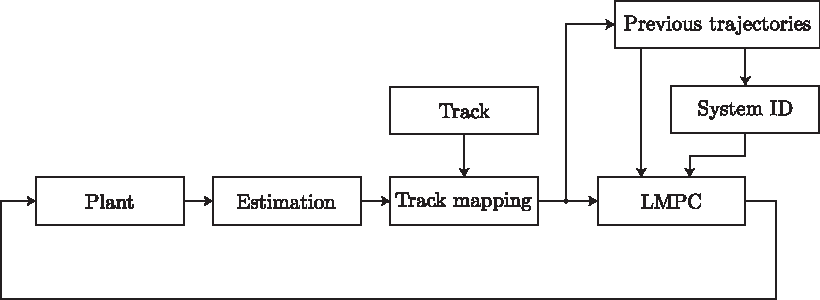
\includegraphics{../../Figures/Illustrator/ControlDiagram.pdf}
%    \caption{Control structure}
%    \label{fig:controlStructure}
%\end{figure}

\section{Introduction to the BARC}
The car used for our experiments is a remote controlled race car of the model "Basher RZ-4 1/10 Rally Racer" that has been modified by the MPC Lab at UC Berkeley to easily test new control techniques. This car is called Berkeley Autonomous Race Car (BARC, \cite{BARC}) and it has been used previously in student projects. The basic setup is shown in figure \ref{fig:BARC}.
\begin{figure}[ht]
    \centering
  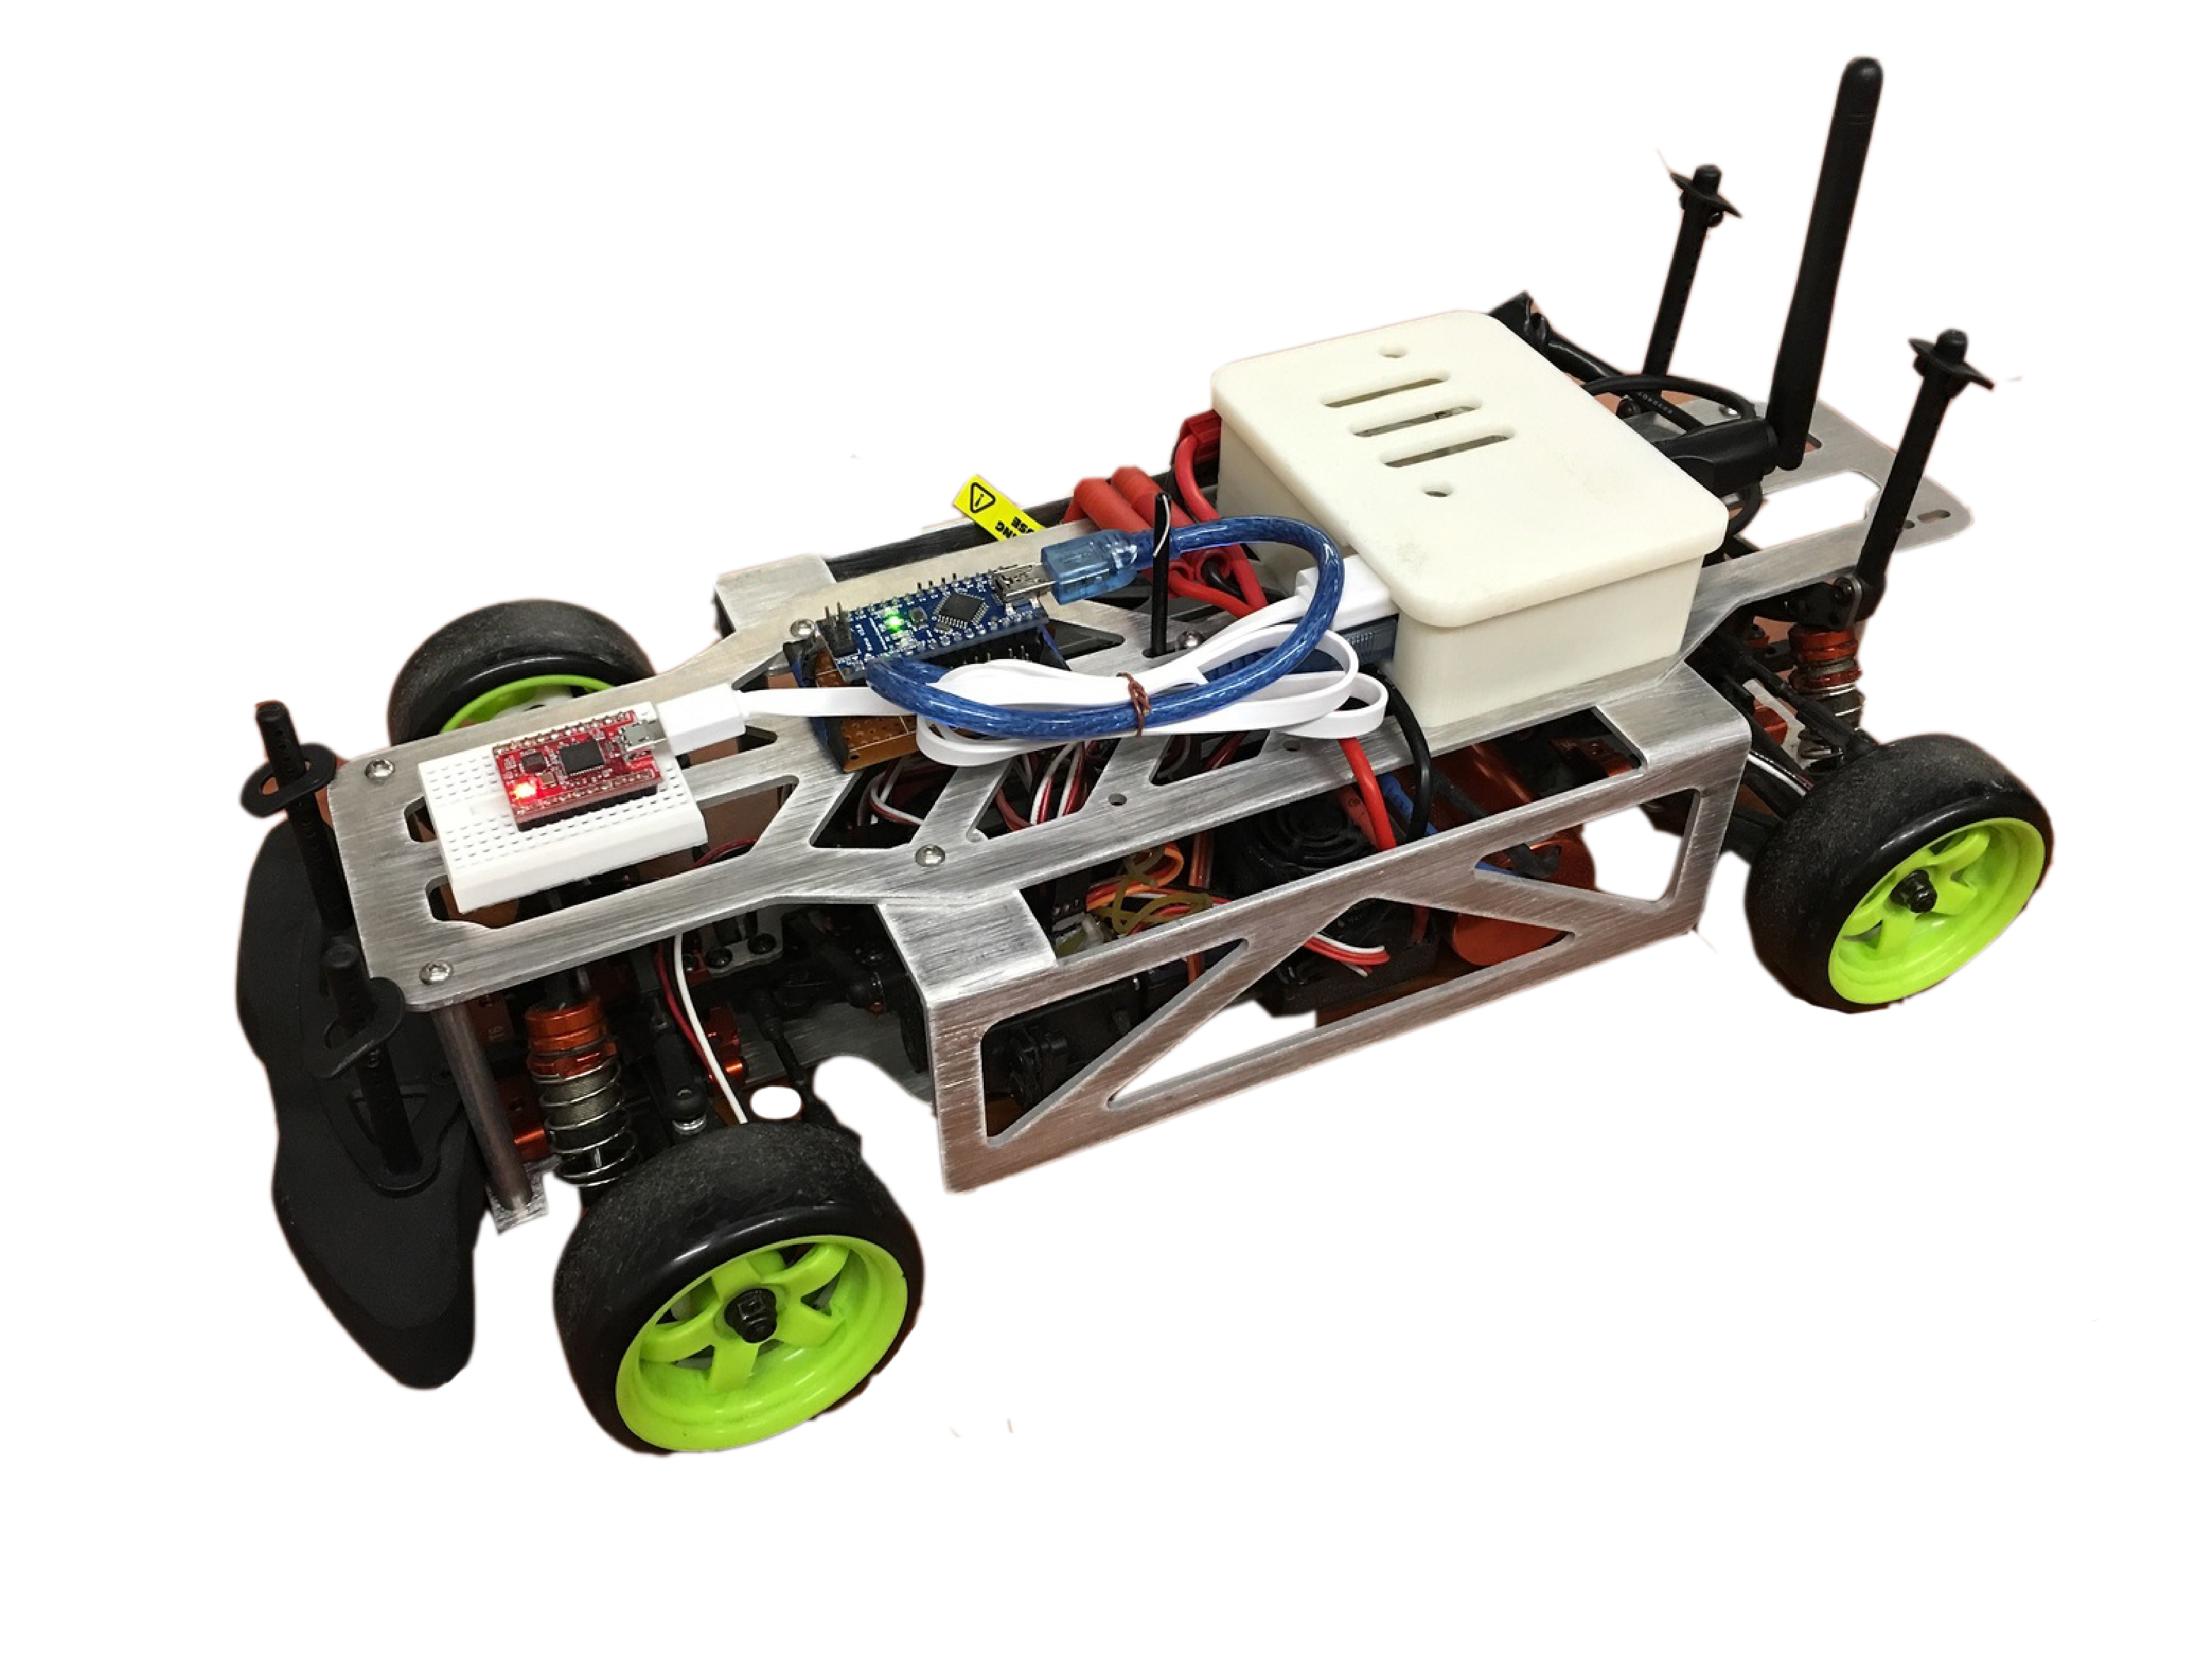
\includegraphics[width=0.8\textwidth]{../../Figures/BARC/IMG_1047.pdf}
    \caption{Basic BARC setup}
    \label{fig:BARC}
\end{figure}

Aside from standard actuators (brushless DC motor and steering servo), it features two onboard CPUs. The first CPU is an Arduino Nano which allows low-level control of the actuators as well as receiving and simple processing of sensor data. The second CPU is a Samsung Exynos 5422, provided by an Odroid XU4 single board computer. The Exynos CPU family has been used since 2010 on various smartphones like the Samsung Galaxy S. This processor is used for high-level computing (i.e. communication with USB devices and an external computer).
\subsection{Sensors}
For the purpose of race driving the estimation of absolute position, velocity and orientation are needed. The goal of the BARC project is to provide an affordable solution that can be used for testing autonomous driving algorithms. To accomplish this goal the following low cost  sensors were chosen:
\begin{description}
\item[IMU] The Inertial Measurement Unit measures linear and angular accelerations as well as the car's current orientation in space. The IMU used on the BARC is a myAHRS+ which runs at a frequency of 50 Hertz. It is directly connected to the Odroid through a USB port.
\item[Encoders] Each wheel contains two magnetically operating encoders which can be used to measure the car's velocity. These measurements are only reliable as long as the car is not drifting and as long as the wheels are spinning. The frequency of these measurements is directly related to the rotating speed of the wheels. The encoders are connected to the arduino and send a signal at each half spin of the wheel. The arduino sends the average speed resulting form the signals to the odroid.
% Yes, actually there are 4 encoders, but we are only able to use two of them.
\item[GPS] To determine the absolute position of the car, an indoor positioning system from \emph{Marvelmind robotics} \cite{marvelmind} is used. Similar to the Global Positioning System (GPS), it determines the position of the car by triangulating the distances between stationary beacons around the racetrack and a mobile beacon which is fixed to the car. Distances are measured by the time of flight of ultrasound signals between all beacons.\\
The system measures the position with deviations of about $\SI{2}{\centi\meter}$ at a varying frequency between 10 and 16 Hertz.
\end{description}

\subsection{Input mapping}\label{sec:inputMapping}
While the MPC formulation calculates inputs of acceleration and steering in SI units, the actuators are controlled by the Arduino using pulse-width-modulation (PWM) signals. This section describes the identification procedure to find the steering mapping and acceleration mapping.
%{\bfseries{I noticed that sometime the sentences are a bit convolute, it is good practice to make them as simple and short as possible (I sill have lot of problems in doing that). For instance I would reformulate your last sentence: "This section describes the identification champaign to find the steering and acceleration mapping."}}
\paragraph{Steering mapping}%{\bfseries{Is the the official template for the MS or you made it? I would ask the professor that is going to read the thesis if there is a standard latex template --> mb: Yes it is the standard template}}
To identify the steering mapping, different steering PWM signals are sent to the steering servo while driving at a constant acceleration signal. Due to electromagnetic motor drag, this leads to a constant velocity while performing circles of different radii. A low velocity is used so that an ideal kinematic bicycle model can be assumed. Using the equations of the kinematic bicycle model, the steering angle $\delta_F$ can be inferred:
\begin{equation}\label{eq:deltaF}
\delta_F = \arctan\left(\frac{\dot\psi\cdot(L_F+L_R)}{v_x}\right)
\end{equation}
It can be seen that only $\dot \psi$ and $v_x$ need to be measured to calculate $\delta_F$. Both quantities are measured with good accuracy by the IMU and encoders.
Running this open loop test and approximating the measurements with an affine function, following results are obtained:
\begin{equation}
u_{PWM} = 89.8\cdot \delta_F + 90.8
\end{equation}
\begin{figure}[ht]
    \centering
  %% Creator: Matplotlib, PGF backend
%%
%% To include the figure in your LaTeX document, write
%%   \input{<filename>.pgf}
%%
%% Make sure the required packages are loaded in your preamble
%%   \usepackage{pgf}
%%
%% Figures using additional raster images can only be included by \input if
%% they are in the same directory as the main LaTeX file. For loading figures
%% from other directories you can use the `import` package
%%   \usepackage{import}
%% and then include the figures with
%%   \import{<path to file>}{<filename>.pgf}
%%
%% Matplotlib used the following preamble
%%   \usepackage{fontspec}
%%
\begingroup%
\makeatletter%
\begin{pgfpicture}%
\pgfpathrectangle{\pgfpointorigin}{\pgfqpoint{4.500000in}{3.000000in}}%
\pgfusepath{use as bounding box, clip}%
\begin{pgfscope}%
\pgfsetbuttcap%
\pgfsetmiterjoin%
\definecolor{currentfill}{rgb}{1.000000,1.000000,1.000000}%
\pgfsetfillcolor{currentfill}%
\pgfsetlinewidth{0.000000pt}%
\definecolor{currentstroke}{rgb}{1.000000,1.000000,1.000000}%
\pgfsetstrokecolor{currentstroke}%
\pgfsetdash{}{0pt}%
\pgfpathmoveto{\pgfqpoint{0.000000in}{0.000000in}}%
\pgfpathlineto{\pgfqpoint{4.500000in}{0.000000in}}%
\pgfpathlineto{\pgfqpoint{4.500000in}{3.000000in}}%
\pgfpathlineto{\pgfqpoint{0.000000in}{3.000000in}}%
\pgfpathclose%
\pgfusepath{fill}%
\end{pgfscope}%
\begin{pgfscope}%
\pgfsetbuttcap%
\pgfsetmiterjoin%
\definecolor{currentfill}{rgb}{1.000000,1.000000,1.000000}%
\pgfsetfillcolor{currentfill}%
\pgfsetlinewidth{0.000000pt}%
\definecolor{currentstroke}{rgb}{0.000000,0.000000,0.000000}%
\pgfsetstrokecolor{currentstroke}%
\pgfsetstrokeopacity{0.000000}%
\pgfsetdash{}{0pt}%
\pgfpathmoveto{\pgfqpoint{0.628717in}{0.471921in}}%
\pgfpathlineto{\pgfqpoint{4.261975in}{0.471921in}}%
\pgfpathlineto{\pgfqpoint{4.261975in}{2.805251in}}%
\pgfpathlineto{\pgfqpoint{0.628717in}{2.805251in}}%
\pgfpathclose%
\pgfusepath{fill}%
\end{pgfscope}%
\begin{pgfscope}%
\pgfpathrectangle{\pgfqpoint{0.628717in}{0.471921in}}{\pgfqpoint{3.633258in}{2.333330in}} %
\pgfusepath{clip}%
\pgfsetbuttcap%
\pgfsetroundjoin%
\definecolor{currentfill}{rgb}{0.000000,0.000000,1.000000}%
\pgfsetfillcolor{currentfill}%
\pgfsetlinewidth{0.501875pt}%
\definecolor{currentstroke}{rgb}{0.000000,0.000000,1.000000}%
\pgfsetstrokecolor{currentstroke}%
\pgfsetdash{}{0pt}%
\pgfsys@defobject{currentmarker}{\pgfqpoint{-0.013889in}{-0.013889in}}{\pgfqpoint{0.013889in}{0.013889in}}{%
\pgfpathmoveto{\pgfqpoint{-0.013889in}{0.000000in}}%
\pgfpathlineto{\pgfqpoint{0.013889in}{0.000000in}}%
\pgfpathmoveto{\pgfqpoint{0.000000in}{-0.013889in}}%
\pgfpathlineto{\pgfqpoint{0.000000in}{0.013889in}}%
\pgfusepath{stroke,fill}%
}%
\begin{pgfscope}%
\pgfsys@transformshift{0.628717in}{0.724566in}%
\pgfsys@useobject{currentmarker}{}%
\end{pgfscope}%
\begin{pgfscope}%
\pgfsys@transformshift{0.628717in}{0.724566in}%
\pgfsys@useobject{currentmarker}{}%
\end{pgfscope}%
\begin{pgfscope}%
\pgfsys@transformshift{0.628717in}{0.748045in}%
\pgfsys@useobject{currentmarker}{}%
\end{pgfscope}%
\begin{pgfscope}%
\pgfsys@transformshift{0.628717in}{0.746613in}%
\pgfsys@useobject{currentmarker}{}%
\end{pgfscope}%
\begin{pgfscope}%
\pgfsys@transformshift{0.628717in}{0.753158in}%
\pgfsys@useobject{currentmarker}{}%
\end{pgfscope}%
\begin{pgfscope}%
\pgfsys@transformshift{0.628717in}{0.842776in}%
\pgfsys@useobject{currentmarker}{}%
\end{pgfscope}%
\begin{pgfscope}%
\pgfsys@transformshift{0.628717in}{0.799082in}%
\pgfsys@useobject{currentmarker}{}%
\end{pgfscope}%
\begin{pgfscope}%
\pgfsys@transformshift{0.628717in}{0.773954in}%
\pgfsys@useobject{currentmarker}{}%
\end{pgfscope}%
\begin{pgfscope}%
\pgfsys@transformshift{0.628717in}{0.838914in}%
\pgfsys@useobject{currentmarker}{}%
\end{pgfscope}%
\begin{pgfscope}%
\pgfsys@transformshift{0.749825in}{0.768101in}%
\pgfsys@useobject{currentmarker}{}%
\end{pgfscope}%
\begin{pgfscope}%
\pgfsys@transformshift{0.749825in}{0.761528in}%
\pgfsys@useobject{currentmarker}{}%
\end{pgfscope}%
\begin{pgfscope}%
\pgfsys@transformshift{0.749825in}{0.734944in}%
\pgfsys@useobject{currentmarker}{}%
\end{pgfscope}%
\begin{pgfscope}%
\pgfsys@transformshift{0.749825in}{0.760476in}%
\pgfsys@useobject{currentmarker}{}%
\end{pgfscope}%
\begin{pgfscope}%
\pgfsys@transformshift{0.749825in}{0.818390in}%
\pgfsys@useobject{currentmarker}{}%
\end{pgfscope}%
\begin{pgfscope}%
\pgfsys@transformshift{0.749825in}{0.766250in}%
\pgfsys@useobject{currentmarker}{}%
\end{pgfscope}%
\begin{pgfscope}%
\pgfsys@transformshift{0.749825in}{0.755789in}%
\pgfsys@useobject{currentmarker}{}%
\end{pgfscope}%
\begin{pgfscope}%
\pgfsys@transformshift{0.749825in}{0.814814in}%
\pgfsys@useobject{currentmarker}{}%
\end{pgfscope}%
\begin{pgfscope}%
\pgfsys@transformshift{0.870934in}{0.804724in}%
\pgfsys@useobject{currentmarker}{}%
\end{pgfscope}%
\begin{pgfscope}%
\pgfsys@transformshift{0.870934in}{0.804724in}%
\pgfsys@useobject{currentmarker}{}%
\end{pgfscope}%
\begin{pgfscope}%
\pgfsys@transformshift{0.870934in}{0.804724in}%
\pgfsys@useobject{currentmarker}{}%
\end{pgfscope}%
\begin{pgfscope}%
\pgfsys@transformshift{0.870934in}{0.804724in}%
\pgfsys@useobject{currentmarker}{}%
\end{pgfscope}%
\begin{pgfscope}%
\pgfsys@transformshift{0.870934in}{0.804724in}%
\pgfsys@useobject{currentmarker}{}%
\end{pgfscope}%
\begin{pgfscope}%
\pgfsys@transformshift{0.870934in}{0.804724in}%
\pgfsys@useobject{currentmarker}{}%
\end{pgfscope}%
\begin{pgfscope}%
\pgfsys@transformshift{0.870934in}{0.804724in}%
\pgfsys@useobject{currentmarker}{}%
\end{pgfscope}%
\begin{pgfscope}%
\pgfsys@transformshift{0.870934in}{0.804724in}%
\pgfsys@useobject{currentmarker}{}%
\end{pgfscope}%
\begin{pgfscope}%
\pgfsys@transformshift{0.870934in}{0.804724in}%
\pgfsys@useobject{currentmarker}{}%
\end{pgfscope}%
\begin{pgfscope}%
\pgfsys@transformshift{0.870934in}{0.804724in}%
\pgfsys@useobject{currentmarker}{}%
\end{pgfscope}%
\begin{pgfscope}%
\pgfsys@transformshift{0.870934in}{0.804724in}%
\pgfsys@useobject{currentmarker}{}%
\end{pgfscope}%
\begin{pgfscope}%
\pgfsys@transformshift{0.870934in}{0.804724in}%
\pgfsys@useobject{currentmarker}{}%
\end{pgfscope}%
\begin{pgfscope}%
\pgfsys@transformshift{0.870934in}{0.832525in}%
\pgfsys@useobject{currentmarker}{}%
\end{pgfscope}%
\begin{pgfscope}%
\pgfsys@transformshift{0.870934in}{0.815966in}%
\pgfsys@useobject{currentmarker}{}%
\end{pgfscope}%
\begin{pgfscope}%
\pgfsys@transformshift{0.870934in}{0.847444in}%
\pgfsys@useobject{currentmarker}{}%
\end{pgfscope}%
\begin{pgfscope}%
\pgfsys@transformshift{0.870934in}{0.869380in}%
\pgfsys@useobject{currentmarker}{}%
\end{pgfscope}%
\begin{pgfscope}%
\pgfsys@transformshift{0.870934in}{0.935507in}%
\pgfsys@useobject{currentmarker}{}%
\end{pgfscope}%
\begin{pgfscope}%
\pgfsys@transformshift{0.870934in}{0.838458in}%
\pgfsys@useobject{currentmarker}{}%
\end{pgfscope}%
\begin{pgfscope}%
\pgfsys@transformshift{0.870934in}{0.838458in}%
\pgfsys@useobject{currentmarker}{}%
\end{pgfscope}%
\begin{pgfscope}%
\pgfsys@transformshift{0.870934in}{0.838458in}%
\pgfsys@useobject{currentmarker}{}%
\end{pgfscope}%
\begin{pgfscope}%
\pgfsys@transformshift{0.870934in}{0.838458in}%
\pgfsys@useobject{currentmarker}{}%
\end{pgfscope}%
\begin{pgfscope}%
\pgfsys@transformshift{0.870934in}{0.838458in}%
\pgfsys@useobject{currentmarker}{}%
\end{pgfscope}%
\begin{pgfscope}%
\pgfsys@transformshift{0.870934in}{0.838458in}%
\pgfsys@useobject{currentmarker}{}%
\end{pgfscope}%
\begin{pgfscope}%
\pgfsys@transformshift{0.870934in}{0.838458in}%
\pgfsys@useobject{currentmarker}{}%
\end{pgfscope}%
\begin{pgfscope}%
\pgfsys@transformshift{0.870934in}{0.838458in}%
\pgfsys@useobject{currentmarker}{}%
\end{pgfscope}%
\begin{pgfscope}%
\pgfsys@transformshift{0.870934in}{0.838458in}%
\pgfsys@useobject{currentmarker}{}%
\end{pgfscope}%
\begin{pgfscope}%
\pgfsys@transformshift{0.870934in}{0.838458in}%
\pgfsys@useobject{currentmarker}{}%
\end{pgfscope}%
\begin{pgfscope}%
\pgfsys@transformshift{0.870934in}{0.838458in}%
\pgfsys@useobject{currentmarker}{}%
\end{pgfscope}%
\begin{pgfscope}%
\pgfsys@transformshift{0.870934in}{0.839662in}%
\pgfsys@useobject{currentmarker}{}%
\end{pgfscope}%
\begin{pgfscope}%
\pgfsys@transformshift{0.870934in}{0.839662in}%
\pgfsys@useobject{currentmarker}{}%
\end{pgfscope}%
\begin{pgfscope}%
\pgfsys@transformshift{0.870934in}{0.839662in}%
\pgfsys@useobject{currentmarker}{}%
\end{pgfscope}%
\begin{pgfscope}%
\pgfsys@transformshift{0.870934in}{0.839662in}%
\pgfsys@useobject{currentmarker}{}%
\end{pgfscope}%
\begin{pgfscope}%
\pgfsys@transformshift{0.870934in}{0.839662in}%
\pgfsys@useobject{currentmarker}{}%
\end{pgfscope}%
\begin{pgfscope}%
\pgfsys@transformshift{0.870934in}{0.839662in}%
\pgfsys@useobject{currentmarker}{}%
\end{pgfscope}%
\begin{pgfscope}%
\pgfsys@transformshift{0.870934in}{0.836345in}%
\pgfsys@useobject{currentmarker}{}%
\end{pgfscope}%
\begin{pgfscope}%
\pgfsys@transformshift{0.870934in}{0.795381in}%
\pgfsys@useobject{currentmarker}{}%
\end{pgfscope}%
\begin{pgfscope}%
\pgfsys@transformshift{0.870934in}{0.795381in}%
\pgfsys@useobject{currentmarker}{}%
\end{pgfscope}%
\begin{pgfscope}%
\pgfsys@transformshift{0.870934in}{0.795381in}%
\pgfsys@useobject{currentmarker}{}%
\end{pgfscope}%
\begin{pgfscope}%
\pgfsys@transformshift{0.870934in}{0.795381in}%
\pgfsys@useobject{currentmarker}{}%
\end{pgfscope}%
\begin{pgfscope}%
\pgfsys@transformshift{0.870934in}{0.795381in}%
\pgfsys@useobject{currentmarker}{}%
\end{pgfscope}%
\begin{pgfscope}%
\pgfsys@transformshift{0.870934in}{0.795381in}%
\pgfsys@useobject{currentmarker}{}%
\end{pgfscope}%
\begin{pgfscope}%
\pgfsys@transformshift{0.870934in}{0.795381in}%
\pgfsys@useobject{currentmarker}{}%
\end{pgfscope}%
\begin{pgfscope}%
\pgfsys@transformshift{0.870934in}{0.795381in}%
\pgfsys@useobject{currentmarker}{}%
\end{pgfscope}%
\begin{pgfscope}%
\pgfsys@transformshift{0.870934in}{0.795381in}%
\pgfsys@useobject{currentmarker}{}%
\end{pgfscope}%
\begin{pgfscope}%
\pgfsys@transformshift{0.870934in}{0.795381in}%
\pgfsys@useobject{currentmarker}{}%
\end{pgfscope}%
\begin{pgfscope}%
\pgfsys@transformshift{0.870934in}{0.795381in}%
\pgfsys@useobject{currentmarker}{}%
\end{pgfscope}%
\begin{pgfscope}%
\pgfsys@transformshift{0.870934in}{0.795381in}%
\pgfsys@useobject{currentmarker}{}%
\end{pgfscope}%
\begin{pgfscope}%
\pgfsys@transformshift{0.870934in}{0.795381in}%
\pgfsys@useobject{currentmarker}{}%
\end{pgfscope}%
\begin{pgfscope}%
\pgfsys@transformshift{0.870934in}{0.795381in}%
\pgfsys@useobject{currentmarker}{}%
\end{pgfscope}%
\begin{pgfscope}%
\pgfsys@transformshift{0.870934in}{0.809233in}%
\pgfsys@useobject{currentmarker}{}%
\end{pgfscope}%
\begin{pgfscope}%
\pgfsys@transformshift{0.870934in}{0.816012in}%
\pgfsys@useobject{currentmarker}{}%
\end{pgfscope}%
\begin{pgfscope}%
\pgfsys@transformshift{0.870934in}{0.848175in}%
\pgfsys@useobject{currentmarker}{}%
\end{pgfscope}%
\begin{pgfscope}%
\pgfsys@transformshift{0.870934in}{0.859195in}%
\pgfsys@useobject{currentmarker}{}%
\end{pgfscope}%
\begin{pgfscope}%
\pgfsys@transformshift{0.870934in}{0.859195in}%
\pgfsys@useobject{currentmarker}{}%
\end{pgfscope}%
\begin{pgfscope}%
\pgfsys@transformshift{0.870934in}{0.850114in}%
\pgfsys@useobject{currentmarker}{}%
\end{pgfscope}%
\begin{pgfscope}%
\pgfsys@transformshift{0.870934in}{0.850114in}%
\pgfsys@useobject{currentmarker}{}%
\end{pgfscope}%
\begin{pgfscope}%
\pgfsys@transformshift{0.870934in}{0.850114in}%
\pgfsys@useobject{currentmarker}{}%
\end{pgfscope}%
\begin{pgfscope}%
\pgfsys@transformshift{0.870934in}{0.850114in}%
\pgfsys@useobject{currentmarker}{}%
\end{pgfscope}%
\begin{pgfscope}%
\pgfsys@transformshift{0.870934in}{0.850114in}%
\pgfsys@useobject{currentmarker}{}%
\end{pgfscope}%
\begin{pgfscope}%
\pgfsys@transformshift{0.870934in}{0.850114in}%
\pgfsys@useobject{currentmarker}{}%
\end{pgfscope}%
\begin{pgfscope}%
\pgfsys@transformshift{0.870934in}{0.850114in}%
\pgfsys@useobject{currentmarker}{}%
\end{pgfscope}%
\begin{pgfscope}%
\pgfsys@transformshift{0.870934in}{0.850114in}%
\pgfsys@useobject{currentmarker}{}%
\end{pgfscope}%
\begin{pgfscope}%
\pgfsys@transformshift{0.870934in}{0.850114in}%
\pgfsys@useobject{currentmarker}{}%
\end{pgfscope}%
\begin{pgfscope}%
\pgfsys@transformshift{0.870934in}{0.850114in}%
\pgfsys@useobject{currentmarker}{}%
\end{pgfscope}%
\begin{pgfscope}%
\pgfsys@transformshift{0.870934in}{0.850114in}%
\pgfsys@useobject{currentmarker}{}%
\end{pgfscope}%
\begin{pgfscope}%
\pgfsys@transformshift{0.870934in}{0.850114in}%
\pgfsys@useobject{currentmarker}{}%
\end{pgfscope}%
\begin{pgfscope}%
\pgfsys@transformshift{0.870934in}{0.850114in}%
\pgfsys@useobject{currentmarker}{}%
\end{pgfscope}%
\begin{pgfscope}%
\pgfsys@transformshift{0.870934in}{0.871689in}%
\pgfsys@useobject{currentmarker}{}%
\end{pgfscope}%
\begin{pgfscope}%
\pgfsys@transformshift{0.870934in}{0.871689in}%
\pgfsys@useobject{currentmarker}{}%
\end{pgfscope}%
\begin{pgfscope}%
\pgfsys@transformshift{0.870934in}{0.871689in}%
\pgfsys@useobject{currentmarker}{}%
\end{pgfscope}%
\begin{pgfscope}%
\pgfsys@transformshift{0.870934in}{0.871689in}%
\pgfsys@useobject{currentmarker}{}%
\end{pgfscope}%
\begin{pgfscope}%
\pgfsys@transformshift{0.870934in}{0.871689in}%
\pgfsys@useobject{currentmarker}{}%
\end{pgfscope}%
\begin{pgfscope}%
\pgfsys@transformshift{0.870934in}{0.871689in}%
\pgfsys@useobject{currentmarker}{}%
\end{pgfscope}%
\begin{pgfscope}%
\pgfsys@transformshift{0.870934in}{0.871689in}%
\pgfsys@useobject{currentmarker}{}%
\end{pgfscope}%
\begin{pgfscope}%
\pgfsys@transformshift{0.870934in}{0.871689in}%
\pgfsys@useobject{currentmarker}{}%
\end{pgfscope}%
\begin{pgfscope}%
\pgfsys@transformshift{0.870934in}{0.871689in}%
\pgfsys@useobject{currentmarker}{}%
\end{pgfscope}%
\begin{pgfscope}%
\pgfsys@transformshift{0.870934in}{0.871689in}%
\pgfsys@useobject{currentmarker}{}%
\end{pgfscope}%
\begin{pgfscope}%
\pgfsys@transformshift{0.870934in}{0.871689in}%
\pgfsys@useobject{currentmarker}{}%
\end{pgfscope}%
\begin{pgfscope}%
\pgfsys@transformshift{0.870934in}{0.871689in}%
\pgfsys@useobject{currentmarker}{}%
\end{pgfscope}%
\begin{pgfscope}%
\pgfsys@transformshift{0.870934in}{0.871689in}%
\pgfsys@useobject{currentmarker}{}%
\end{pgfscope}%
\begin{pgfscope}%
\pgfsys@transformshift{0.870934in}{0.871689in}%
\pgfsys@useobject{currentmarker}{}%
\end{pgfscope}%
\begin{pgfscope}%
\pgfsys@transformshift{0.870934in}{0.871689in}%
\pgfsys@useobject{currentmarker}{}%
\end{pgfscope}%
\begin{pgfscope}%
\pgfsys@transformshift{0.870934in}{0.871689in}%
\pgfsys@useobject{currentmarker}{}%
\end{pgfscope}%
\begin{pgfscope}%
\pgfsys@transformshift{0.870934in}{0.871689in}%
\pgfsys@useobject{currentmarker}{}%
\end{pgfscope}%
\begin{pgfscope}%
\pgfsys@transformshift{0.870934in}{0.871689in}%
\pgfsys@useobject{currentmarker}{}%
\end{pgfscope}%
\begin{pgfscope}%
\pgfsys@transformshift{0.870934in}{0.871689in}%
\pgfsys@useobject{currentmarker}{}%
\end{pgfscope}%
\begin{pgfscope}%
\pgfsys@transformshift{0.870934in}{0.871689in}%
\pgfsys@useobject{currentmarker}{}%
\end{pgfscope}%
\begin{pgfscope}%
\pgfsys@transformshift{0.870934in}{0.871689in}%
\pgfsys@useobject{currentmarker}{}%
\end{pgfscope}%
\begin{pgfscope}%
\pgfsys@transformshift{0.870934in}{0.826315in}%
\pgfsys@useobject{currentmarker}{}%
\end{pgfscope}%
\begin{pgfscope}%
\pgfsys@transformshift{0.870934in}{0.826315in}%
\pgfsys@useobject{currentmarker}{}%
\end{pgfscope}%
\begin{pgfscope}%
\pgfsys@transformshift{0.870934in}{0.822983in}%
\pgfsys@useobject{currentmarker}{}%
\end{pgfscope}%
\begin{pgfscope}%
\pgfsys@transformshift{0.870934in}{0.822983in}%
\pgfsys@useobject{currentmarker}{}%
\end{pgfscope}%
\begin{pgfscope}%
\pgfsys@transformshift{0.870934in}{0.822983in}%
\pgfsys@useobject{currentmarker}{}%
\end{pgfscope}%
\begin{pgfscope}%
\pgfsys@transformshift{0.870934in}{0.822983in}%
\pgfsys@useobject{currentmarker}{}%
\end{pgfscope}%
\begin{pgfscope}%
\pgfsys@transformshift{0.870934in}{0.822983in}%
\pgfsys@useobject{currentmarker}{}%
\end{pgfscope}%
\begin{pgfscope}%
\pgfsys@transformshift{0.870934in}{0.822983in}%
\pgfsys@useobject{currentmarker}{}%
\end{pgfscope}%
\begin{pgfscope}%
\pgfsys@transformshift{0.870934in}{0.822983in}%
\pgfsys@useobject{currentmarker}{}%
\end{pgfscope}%
\begin{pgfscope}%
\pgfsys@transformshift{0.870934in}{0.822983in}%
\pgfsys@useobject{currentmarker}{}%
\end{pgfscope}%
\begin{pgfscope}%
\pgfsys@transformshift{0.870934in}{0.822983in}%
\pgfsys@useobject{currentmarker}{}%
\end{pgfscope}%
\begin{pgfscope}%
\pgfsys@transformshift{0.870934in}{0.822983in}%
\pgfsys@useobject{currentmarker}{}%
\end{pgfscope}%
\begin{pgfscope}%
\pgfsys@transformshift{0.870934in}{0.822983in}%
\pgfsys@useobject{currentmarker}{}%
\end{pgfscope}%
\begin{pgfscope}%
\pgfsys@transformshift{0.870934in}{0.822983in}%
\pgfsys@useobject{currentmarker}{}%
\end{pgfscope}%
\begin{pgfscope}%
\pgfsys@transformshift{0.870934in}{0.822983in}%
\pgfsys@useobject{currentmarker}{}%
\end{pgfscope}%
\begin{pgfscope}%
\pgfsys@transformshift{0.870934in}{0.822983in}%
\pgfsys@useobject{currentmarker}{}%
\end{pgfscope}%
\begin{pgfscope}%
\pgfsys@transformshift{0.870934in}{0.822983in}%
\pgfsys@useobject{currentmarker}{}%
\end{pgfscope}%
\begin{pgfscope}%
\pgfsys@transformshift{0.870934in}{0.822983in}%
\pgfsys@useobject{currentmarker}{}%
\end{pgfscope}%
\begin{pgfscope}%
\pgfsys@transformshift{0.870934in}{0.822983in}%
\pgfsys@useobject{currentmarker}{}%
\end{pgfscope}%
\begin{pgfscope}%
\pgfsys@transformshift{0.870934in}{0.822983in}%
\pgfsys@useobject{currentmarker}{}%
\end{pgfscope}%
\begin{pgfscope}%
\pgfsys@transformshift{0.870934in}{0.822983in}%
\pgfsys@useobject{currentmarker}{}%
\end{pgfscope}%
\begin{pgfscope}%
\pgfsys@transformshift{0.870934in}{0.822983in}%
\pgfsys@useobject{currentmarker}{}%
\end{pgfscope}%
\begin{pgfscope}%
\pgfsys@transformshift{0.870934in}{0.822983in}%
\pgfsys@useobject{currentmarker}{}%
\end{pgfscope}%
\begin{pgfscope}%
\pgfsys@transformshift{0.870934in}{0.822983in}%
\pgfsys@useobject{currentmarker}{}%
\end{pgfscope}%
\begin{pgfscope}%
\pgfsys@transformshift{0.870934in}{0.822983in}%
\pgfsys@useobject{currentmarker}{}%
\end{pgfscope}%
\begin{pgfscope}%
\pgfsys@transformshift{0.870934in}{0.822983in}%
\pgfsys@useobject{currentmarker}{}%
\end{pgfscope}%
\begin{pgfscope}%
\pgfsys@transformshift{0.870934in}{0.822983in}%
\pgfsys@useobject{currentmarker}{}%
\end{pgfscope}%
\begin{pgfscope}%
\pgfsys@transformshift{0.870934in}{0.822983in}%
\pgfsys@useobject{currentmarker}{}%
\end{pgfscope}%
\begin{pgfscope}%
\pgfsys@transformshift{0.870934in}{0.822983in}%
\pgfsys@useobject{currentmarker}{}%
\end{pgfscope}%
\begin{pgfscope}%
\pgfsys@transformshift{0.870934in}{0.822983in}%
\pgfsys@useobject{currentmarker}{}%
\end{pgfscope}%
\begin{pgfscope}%
\pgfsys@transformshift{0.870934in}{0.822983in}%
\pgfsys@useobject{currentmarker}{}%
\end{pgfscope}%
\begin{pgfscope}%
\pgfsys@transformshift{0.870934in}{0.822983in}%
\pgfsys@useobject{currentmarker}{}%
\end{pgfscope}%
\begin{pgfscope}%
\pgfsys@transformshift{0.870934in}{0.822983in}%
\pgfsys@useobject{currentmarker}{}%
\end{pgfscope}%
\begin{pgfscope}%
\pgfsys@transformshift{0.870934in}{0.822983in}%
\pgfsys@useobject{currentmarker}{}%
\end{pgfscope}%
\begin{pgfscope}%
\pgfsys@transformshift{0.870934in}{0.822983in}%
\pgfsys@useobject{currentmarker}{}%
\end{pgfscope}%
\begin{pgfscope}%
\pgfsys@transformshift{0.870934in}{0.822983in}%
\pgfsys@useobject{currentmarker}{}%
\end{pgfscope}%
\begin{pgfscope}%
\pgfsys@transformshift{0.870934in}{0.822983in}%
\pgfsys@useobject{currentmarker}{}%
\end{pgfscope}%
\begin{pgfscope}%
\pgfsys@transformshift{0.870934in}{0.822983in}%
\pgfsys@useobject{currentmarker}{}%
\end{pgfscope}%
\begin{pgfscope}%
\pgfsys@transformshift{0.870934in}{0.822983in}%
\pgfsys@useobject{currentmarker}{}%
\end{pgfscope}%
\begin{pgfscope}%
\pgfsys@transformshift{0.870934in}{0.822983in}%
\pgfsys@useobject{currentmarker}{}%
\end{pgfscope}%
\begin{pgfscope}%
\pgfsys@transformshift{0.870934in}{0.822983in}%
\pgfsys@useobject{currentmarker}{}%
\end{pgfscope}%
\begin{pgfscope}%
\pgfsys@transformshift{0.870934in}{0.822983in}%
\pgfsys@useobject{currentmarker}{}%
\end{pgfscope}%
\begin{pgfscope}%
\pgfsys@transformshift{0.870934in}{0.822983in}%
\pgfsys@useobject{currentmarker}{}%
\end{pgfscope}%
\begin{pgfscope}%
\pgfsys@transformshift{0.870934in}{0.822983in}%
\pgfsys@useobject{currentmarker}{}%
\end{pgfscope}%
\begin{pgfscope}%
\pgfsys@transformshift{0.870934in}{0.822983in}%
\pgfsys@useobject{currentmarker}{}%
\end{pgfscope}%
\begin{pgfscope}%
\pgfsys@transformshift{0.870934in}{0.822983in}%
\pgfsys@useobject{currentmarker}{}%
\end{pgfscope}%
\begin{pgfscope}%
\pgfsys@transformshift{0.870934in}{0.822983in}%
\pgfsys@useobject{currentmarker}{}%
\end{pgfscope}%
\begin{pgfscope}%
\pgfsys@transformshift{0.870934in}{0.822983in}%
\pgfsys@useobject{currentmarker}{}%
\end{pgfscope}%
\begin{pgfscope}%
\pgfsys@transformshift{0.870934in}{0.822983in}%
\pgfsys@useobject{currentmarker}{}%
\end{pgfscope}%
\begin{pgfscope}%
\pgfsys@transformshift{0.870934in}{0.822983in}%
\pgfsys@useobject{currentmarker}{}%
\end{pgfscope}%
\begin{pgfscope}%
\pgfsys@transformshift{0.870934in}{0.822983in}%
\pgfsys@useobject{currentmarker}{}%
\end{pgfscope}%
\begin{pgfscope}%
\pgfsys@transformshift{0.870934in}{0.822983in}%
\pgfsys@useobject{currentmarker}{}%
\end{pgfscope}%
\begin{pgfscope}%
\pgfsys@transformshift{0.870934in}{0.822983in}%
\pgfsys@useobject{currentmarker}{}%
\end{pgfscope}%
\begin{pgfscope}%
\pgfsys@transformshift{0.870934in}{0.822983in}%
\pgfsys@useobject{currentmarker}{}%
\end{pgfscope}%
\begin{pgfscope}%
\pgfsys@transformshift{0.870934in}{0.822983in}%
\pgfsys@useobject{currentmarker}{}%
\end{pgfscope}%
\begin{pgfscope}%
\pgfsys@transformshift{0.870934in}{0.822983in}%
\pgfsys@useobject{currentmarker}{}%
\end{pgfscope}%
\begin{pgfscope}%
\pgfsys@transformshift{0.870934in}{0.822983in}%
\pgfsys@useobject{currentmarker}{}%
\end{pgfscope}%
\begin{pgfscope}%
\pgfsys@transformshift{0.870934in}{0.822983in}%
\pgfsys@useobject{currentmarker}{}%
\end{pgfscope}%
\begin{pgfscope}%
\pgfsys@transformshift{0.870934in}{0.822983in}%
\pgfsys@useobject{currentmarker}{}%
\end{pgfscope}%
\begin{pgfscope}%
\pgfsys@transformshift{0.870934in}{0.822983in}%
\pgfsys@useobject{currentmarker}{}%
\end{pgfscope}%
\begin{pgfscope}%
\pgfsys@transformshift{0.870934in}{0.822983in}%
\pgfsys@useobject{currentmarker}{}%
\end{pgfscope}%
\begin{pgfscope}%
\pgfsys@transformshift{0.870934in}{0.822983in}%
\pgfsys@useobject{currentmarker}{}%
\end{pgfscope}%
\begin{pgfscope}%
\pgfsys@transformshift{0.870934in}{0.822983in}%
\pgfsys@useobject{currentmarker}{}%
\end{pgfscope}%
\begin{pgfscope}%
\pgfsys@transformshift{0.870934in}{0.822983in}%
\pgfsys@useobject{currentmarker}{}%
\end{pgfscope}%
\begin{pgfscope}%
\pgfsys@transformshift{0.992043in}{0.876310in}%
\pgfsys@useobject{currentmarker}{}%
\end{pgfscope}%
\begin{pgfscope}%
\pgfsys@transformshift{0.992043in}{0.871201in}%
\pgfsys@useobject{currentmarker}{}%
\end{pgfscope}%
\begin{pgfscope}%
\pgfsys@transformshift{0.992043in}{0.891655in}%
\pgfsys@useobject{currentmarker}{}%
\end{pgfscope}%
\begin{pgfscope}%
\pgfsys@transformshift{0.992043in}{0.923064in}%
\pgfsys@useobject{currentmarker}{}%
\end{pgfscope}%
\begin{pgfscope}%
\pgfsys@transformshift{0.992043in}{0.929695in}%
\pgfsys@useobject{currentmarker}{}%
\end{pgfscope}%
\begin{pgfscope}%
\pgfsys@transformshift{0.992043in}{0.850423in}%
\pgfsys@useobject{currentmarker}{}%
\end{pgfscope}%
\begin{pgfscope}%
\pgfsys@transformshift{0.992043in}{0.874094in}%
\pgfsys@useobject{currentmarker}{}%
\end{pgfscope}%
\begin{pgfscope}%
\pgfsys@transformshift{0.992043in}{0.849784in}%
\pgfsys@useobject{currentmarker}{}%
\end{pgfscope}%
\begin{pgfscope}%
\pgfsys@transformshift{0.992043in}{0.897855in}%
\pgfsys@useobject{currentmarker}{}%
\end{pgfscope}%
\begin{pgfscope}%
\pgfsys@transformshift{0.992043in}{0.922825in}%
\pgfsys@useobject{currentmarker}{}%
\end{pgfscope}%
\begin{pgfscope}%
\pgfsys@transformshift{0.992043in}{0.878743in}%
\pgfsys@useobject{currentmarker}{}%
\end{pgfscope}%
\begin{pgfscope}%
\pgfsys@transformshift{0.992043in}{0.869178in}%
\pgfsys@useobject{currentmarker}{}%
\end{pgfscope}%
\begin{pgfscope}%
\pgfsys@transformshift{0.992043in}{0.869178in}%
\pgfsys@useobject{currentmarker}{}%
\end{pgfscope}%
\begin{pgfscope}%
\pgfsys@transformshift{0.992043in}{0.869178in}%
\pgfsys@useobject{currentmarker}{}%
\end{pgfscope}%
\begin{pgfscope}%
\pgfsys@transformshift{0.992043in}{0.881296in}%
\pgfsys@useobject{currentmarker}{}%
\end{pgfscope}%
\begin{pgfscope}%
\pgfsys@transformshift{0.992043in}{0.919667in}%
\pgfsys@useobject{currentmarker}{}%
\end{pgfscope}%
\begin{pgfscope}%
\pgfsys@transformshift{0.992043in}{0.926466in}%
\pgfsys@useobject{currentmarker}{}%
\end{pgfscope}%
\begin{pgfscope}%
\pgfsys@transformshift{0.992043in}{0.926466in}%
\pgfsys@useobject{currentmarker}{}%
\end{pgfscope}%
\begin{pgfscope}%
\pgfsys@transformshift{0.992043in}{0.934718in}%
\pgfsys@useobject{currentmarker}{}%
\end{pgfscope}%
\begin{pgfscope}%
\pgfsys@transformshift{0.992043in}{0.911250in}%
\pgfsys@useobject{currentmarker}{}%
\end{pgfscope}%
\begin{pgfscope}%
\pgfsys@transformshift{0.992043in}{0.905550in}%
\pgfsys@useobject{currentmarker}{}%
\end{pgfscope}%
\begin{pgfscope}%
\pgfsys@transformshift{0.992043in}{0.900894in}%
\pgfsys@useobject{currentmarker}{}%
\end{pgfscope}%
\begin{pgfscope}%
\pgfsys@transformshift{0.992043in}{0.975702in}%
\pgfsys@useobject{currentmarker}{}%
\end{pgfscope}%
\begin{pgfscope}%
\pgfsys@transformshift{0.992043in}{0.930237in}%
\pgfsys@useobject{currentmarker}{}%
\end{pgfscope}%
\begin{pgfscope}%
\pgfsys@transformshift{0.992043in}{0.962874in}%
\pgfsys@useobject{currentmarker}{}%
\end{pgfscope}%
\begin{pgfscope}%
\pgfsys@transformshift{0.992043in}{0.962874in}%
\pgfsys@useobject{currentmarker}{}%
\end{pgfscope}%
\begin{pgfscope}%
\pgfsys@transformshift{0.992043in}{0.982579in}%
\pgfsys@useobject{currentmarker}{}%
\end{pgfscope}%
\begin{pgfscope}%
\pgfsys@transformshift{0.992043in}{0.989996in}%
\pgfsys@useobject{currentmarker}{}%
\end{pgfscope}%
\begin{pgfscope}%
\pgfsys@transformshift{0.992043in}{0.963049in}%
\pgfsys@useobject{currentmarker}{}%
\end{pgfscope}%
\begin{pgfscope}%
\pgfsys@transformshift{0.992043in}{0.955651in}%
\pgfsys@useobject{currentmarker}{}%
\end{pgfscope}%
\begin{pgfscope}%
\pgfsys@transformshift{0.992043in}{1.020395in}%
\pgfsys@useobject{currentmarker}{}%
\end{pgfscope}%
\begin{pgfscope}%
\pgfsys@transformshift{0.992043in}{1.045452in}%
\pgfsys@useobject{currentmarker}{}%
\end{pgfscope}%
\begin{pgfscope}%
\pgfsys@transformshift{1.355368in}{1.042695in}%
\pgfsys@useobject{currentmarker}{}%
\end{pgfscope}%
\begin{pgfscope}%
\pgfsys@transformshift{1.355368in}{1.017584in}%
\pgfsys@useobject{currentmarker}{}%
\end{pgfscope}%
\begin{pgfscope}%
\pgfsys@transformshift{1.355368in}{0.983741in}%
\pgfsys@useobject{currentmarker}{}%
\end{pgfscope}%
\begin{pgfscope}%
\pgfsys@transformshift{1.355368in}{0.975635in}%
\pgfsys@useobject{currentmarker}{}%
\end{pgfscope}%
\begin{pgfscope}%
\pgfsys@transformshift{1.355368in}{0.977968in}%
\pgfsys@useobject{currentmarker}{}%
\end{pgfscope}%
\begin{pgfscope}%
\pgfsys@transformshift{1.355368in}{1.059878in}%
\pgfsys@useobject{currentmarker}{}%
\end{pgfscope}%
\begin{pgfscope}%
\pgfsys@transformshift{1.355368in}{1.059878in}%
\pgfsys@useobject{currentmarker}{}%
\end{pgfscope}%
\begin{pgfscope}%
\pgfsys@transformshift{1.355368in}{1.036938in}%
\pgfsys@useobject{currentmarker}{}%
\end{pgfscope}%
\begin{pgfscope}%
\pgfsys@transformshift{1.355368in}{1.035590in}%
\pgfsys@useobject{currentmarker}{}%
\end{pgfscope}%
\begin{pgfscope}%
\pgfsys@transformshift{1.355368in}{1.035590in}%
\pgfsys@useobject{currentmarker}{}%
\end{pgfscope}%
\begin{pgfscope}%
\pgfsys@transformshift{1.355368in}{1.017408in}%
\pgfsys@useobject{currentmarker}{}%
\end{pgfscope}%
\begin{pgfscope}%
\pgfsys@transformshift{1.355368in}{1.017408in}%
\pgfsys@useobject{currentmarker}{}%
\end{pgfscope}%
\begin{pgfscope}%
\pgfsys@transformshift{1.355368in}{1.053127in}%
\pgfsys@useobject{currentmarker}{}%
\end{pgfscope}%
\begin{pgfscope}%
\pgfsys@transformshift{1.355368in}{1.055080in}%
\pgfsys@useobject{currentmarker}{}%
\end{pgfscope}%
\begin{pgfscope}%
\pgfsys@transformshift{1.355368in}{1.055080in}%
\pgfsys@useobject{currentmarker}{}%
\end{pgfscope}%
\begin{pgfscope}%
\pgfsys@transformshift{1.355368in}{1.031556in}%
\pgfsys@useobject{currentmarker}{}%
\end{pgfscope}%
\begin{pgfscope}%
\pgfsys@transformshift{1.355368in}{1.031556in}%
\pgfsys@useobject{currentmarker}{}%
\end{pgfscope}%
\begin{pgfscope}%
\pgfsys@transformshift{1.355368in}{1.062483in}%
\pgfsys@useobject{currentmarker}{}%
\end{pgfscope}%
\begin{pgfscope}%
\pgfsys@transformshift{1.355368in}{1.062483in}%
\pgfsys@useobject{currentmarker}{}%
\end{pgfscope}%
\begin{pgfscope}%
\pgfsys@transformshift{1.355368in}{1.077303in}%
\pgfsys@useobject{currentmarker}{}%
\end{pgfscope}%
\begin{pgfscope}%
\pgfsys@transformshift{1.355368in}{1.077303in}%
\pgfsys@useobject{currentmarker}{}%
\end{pgfscope}%
\begin{pgfscope}%
\pgfsys@transformshift{1.355368in}{1.077303in}%
\pgfsys@useobject{currentmarker}{}%
\end{pgfscope}%
\begin{pgfscope}%
\pgfsys@transformshift{1.355368in}{1.046337in}%
\pgfsys@useobject{currentmarker}{}%
\end{pgfscope}%
\begin{pgfscope}%
\pgfsys@transformshift{1.355368in}{1.006071in}%
\pgfsys@useobject{currentmarker}{}%
\end{pgfscope}%
\begin{pgfscope}%
\pgfsys@transformshift{1.355368in}{1.006071in}%
\pgfsys@useobject{currentmarker}{}%
\end{pgfscope}%
\begin{pgfscope}%
\pgfsys@transformshift{1.355368in}{1.007042in}%
\pgfsys@useobject{currentmarker}{}%
\end{pgfscope}%
\begin{pgfscope}%
\pgfsys@transformshift{1.355368in}{0.999047in}%
\pgfsys@useobject{currentmarker}{}%
\end{pgfscope}%
\begin{pgfscope}%
\pgfsys@transformshift{1.355368in}{0.999047in}%
\pgfsys@useobject{currentmarker}{}%
\end{pgfscope}%
\begin{pgfscope}%
\pgfsys@transformshift{1.355368in}{0.992049in}%
\pgfsys@useobject{currentmarker}{}%
\end{pgfscope}%
\begin{pgfscope}%
\pgfsys@transformshift{1.355368in}{0.992049in}%
\pgfsys@useobject{currentmarker}{}%
\end{pgfscope}%
\begin{pgfscope}%
\pgfsys@transformshift{1.355368in}{0.955223in}%
\pgfsys@useobject{currentmarker}{}%
\end{pgfscope}%
\begin{pgfscope}%
\pgfsys@transformshift{1.355368in}{0.955223in}%
\pgfsys@useobject{currentmarker}{}%
\end{pgfscope}%
\begin{pgfscope}%
\pgfsys@transformshift{1.355368in}{1.026450in}%
\pgfsys@useobject{currentmarker}{}%
\end{pgfscope}%
\begin{pgfscope}%
\pgfsys@transformshift{1.355368in}{0.987011in}%
\pgfsys@useobject{currentmarker}{}%
\end{pgfscope}%
\begin{pgfscope}%
\pgfsys@transformshift{1.355368in}{0.968828in}%
\pgfsys@useobject{currentmarker}{}%
\end{pgfscope}%
\begin{pgfscope}%
\pgfsys@transformshift{1.355368in}{1.004598in}%
\pgfsys@useobject{currentmarker}{}%
\end{pgfscope}%
\begin{pgfscope}%
\pgfsys@transformshift{1.355368in}{1.039443in}%
\pgfsys@useobject{currentmarker}{}%
\end{pgfscope}%
\begin{pgfscope}%
\pgfsys@transformshift{1.355368in}{1.012341in}%
\pgfsys@useobject{currentmarker}{}%
\end{pgfscope}%
\begin{pgfscope}%
\pgfsys@transformshift{1.355368in}{0.970248in}%
\pgfsys@useobject{currentmarker}{}%
\end{pgfscope}%
\begin{pgfscope}%
\pgfsys@transformshift{1.355368in}{1.020528in}%
\pgfsys@useobject{currentmarker}{}%
\end{pgfscope}%
\begin{pgfscope}%
\pgfsys@transformshift{1.355368in}{1.053770in}%
\pgfsys@useobject{currentmarker}{}%
\end{pgfscope}%
\begin{pgfscope}%
\pgfsys@transformshift{1.355368in}{1.067609in}%
\pgfsys@useobject{currentmarker}{}%
\end{pgfscope}%
\begin{pgfscope}%
\pgfsys@transformshift{1.355368in}{1.067609in}%
\pgfsys@useobject{currentmarker}{}%
\end{pgfscope}%
\begin{pgfscope}%
\pgfsys@transformshift{1.355368in}{1.067609in}%
\pgfsys@useobject{currentmarker}{}%
\end{pgfscope}%
\begin{pgfscope}%
\pgfsys@transformshift{1.355368in}{1.050099in}%
\pgfsys@useobject{currentmarker}{}%
\end{pgfscope}%
\begin{pgfscope}%
\pgfsys@transformshift{1.355368in}{1.050099in}%
\pgfsys@useobject{currentmarker}{}%
\end{pgfscope}%
\begin{pgfscope}%
\pgfsys@transformshift{1.355368in}{1.050099in}%
\pgfsys@useobject{currentmarker}{}%
\end{pgfscope}%
\begin{pgfscope}%
\pgfsys@transformshift{1.355368in}{1.050099in}%
\pgfsys@useobject{currentmarker}{}%
\end{pgfscope}%
\begin{pgfscope}%
\pgfsys@transformshift{1.355368in}{1.050099in}%
\pgfsys@useobject{currentmarker}{}%
\end{pgfscope}%
\begin{pgfscope}%
\pgfsys@transformshift{1.355368in}{1.050099in}%
\pgfsys@useobject{currentmarker}{}%
\end{pgfscope}%
\begin{pgfscope}%
\pgfsys@transformshift{1.355368in}{1.050099in}%
\pgfsys@useobject{currentmarker}{}%
\end{pgfscope}%
\begin{pgfscope}%
\pgfsys@transformshift{1.355368in}{1.050099in}%
\pgfsys@useobject{currentmarker}{}%
\end{pgfscope}%
\begin{pgfscope}%
\pgfsys@transformshift{1.355368in}{1.050099in}%
\pgfsys@useobject{currentmarker}{}%
\end{pgfscope}%
\begin{pgfscope}%
\pgfsys@transformshift{1.355368in}{1.050099in}%
\pgfsys@useobject{currentmarker}{}%
\end{pgfscope}%
\begin{pgfscope}%
\pgfsys@transformshift{1.355368in}{1.041045in}%
\pgfsys@useobject{currentmarker}{}%
\end{pgfscope}%
\begin{pgfscope}%
\pgfsys@transformshift{1.355368in}{1.041045in}%
\pgfsys@useobject{currentmarker}{}%
\end{pgfscope}%
\begin{pgfscope}%
\pgfsys@transformshift{1.355368in}{1.003715in}%
\pgfsys@useobject{currentmarker}{}%
\end{pgfscope}%
\begin{pgfscope}%
\pgfsys@transformshift{1.355368in}{1.003715in}%
\pgfsys@useobject{currentmarker}{}%
\end{pgfscope}%
\begin{pgfscope}%
\pgfsys@transformshift{1.355368in}{0.995166in}%
\pgfsys@useobject{currentmarker}{}%
\end{pgfscope}%
\begin{pgfscope}%
\pgfsys@transformshift{1.355368in}{0.995166in}%
\pgfsys@useobject{currentmarker}{}%
\end{pgfscope}%
\begin{pgfscope}%
\pgfsys@transformshift{1.355368in}{0.995166in}%
\pgfsys@useobject{currentmarker}{}%
\end{pgfscope}%
\begin{pgfscope}%
\pgfsys@transformshift{1.355368in}{0.954347in}%
\pgfsys@useobject{currentmarker}{}%
\end{pgfscope}%
\begin{pgfscope}%
\pgfsys@transformshift{1.355368in}{0.954347in}%
\pgfsys@useobject{currentmarker}{}%
\end{pgfscope}%
\begin{pgfscope}%
\pgfsys@transformshift{1.355368in}{0.954347in}%
\pgfsys@useobject{currentmarker}{}%
\end{pgfscope}%
\begin{pgfscope}%
\pgfsys@transformshift{1.355368in}{0.954347in}%
\pgfsys@useobject{currentmarker}{}%
\end{pgfscope}%
\begin{pgfscope}%
\pgfsys@transformshift{1.355368in}{0.954347in}%
\pgfsys@useobject{currentmarker}{}%
\end{pgfscope}%
\begin{pgfscope}%
\pgfsys@transformshift{1.355368in}{0.954347in}%
\pgfsys@useobject{currentmarker}{}%
\end{pgfscope}%
\begin{pgfscope}%
\pgfsys@transformshift{1.355368in}{0.940372in}%
\pgfsys@useobject{currentmarker}{}%
\end{pgfscope}%
\begin{pgfscope}%
\pgfsys@transformshift{1.355368in}{0.940372in}%
\pgfsys@useobject{currentmarker}{}%
\end{pgfscope}%
\begin{pgfscope}%
\pgfsys@transformshift{1.355368in}{0.940372in}%
\pgfsys@useobject{currentmarker}{}%
\end{pgfscope}%
\begin{pgfscope}%
\pgfsys@transformshift{1.355368in}{0.940372in}%
\pgfsys@useobject{currentmarker}{}%
\end{pgfscope}%
\begin{pgfscope}%
\pgfsys@transformshift{1.355368in}{0.940372in}%
\pgfsys@useobject{currentmarker}{}%
\end{pgfscope}%
\begin{pgfscope}%
\pgfsys@transformshift{1.355368in}{0.940372in}%
\pgfsys@useobject{currentmarker}{}%
\end{pgfscope}%
\begin{pgfscope}%
\pgfsys@transformshift{1.355368in}{0.940372in}%
\pgfsys@useobject{currentmarker}{}%
\end{pgfscope}%
\begin{pgfscope}%
\pgfsys@transformshift{1.355368in}{0.940372in}%
\pgfsys@useobject{currentmarker}{}%
\end{pgfscope}%
\begin{pgfscope}%
\pgfsys@transformshift{1.355368in}{0.940372in}%
\pgfsys@useobject{currentmarker}{}%
\end{pgfscope}%
\begin{pgfscope}%
\pgfsys@transformshift{1.355368in}{0.940372in}%
\pgfsys@useobject{currentmarker}{}%
\end{pgfscope}%
\begin{pgfscope}%
\pgfsys@transformshift{1.355368in}{0.940372in}%
\pgfsys@useobject{currentmarker}{}%
\end{pgfscope}%
\begin{pgfscope}%
\pgfsys@transformshift{1.355368in}{0.940372in}%
\pgfsys@useobject{currentmarker}{}%
\end{pgfscope}%
\begin{pgfscope}%
\pgfsys@transformshift{1.355368in}{0.940372in}%
\pgfsys@useobject{currentmarker}{}%
\end{pgfscope}%
\begin{pgfscope}%
\pgfsys@transformshift{1.355368in}{0.940372in}%
\pgfsys@useobject{currentmarker}{}%
\end{pgfscope}%
\begin{pgfscope}%
\pgfsys@transformshift{1.355368in}{0.940372in}%
\pgfsys@useobject{currentmarker}{}%
\end{pgfscope}%
\begin{pgfscope}%
\pgfsys@transformshift{1.355368in}{0.940372in}%
\pgfsys@useobject{currentmarker}{}%
\end{pgfscope}%
\begin{pgfscope}%
\pgfsys@transformshift{1.355368in}{1.005548in}%
\pgfsys@useobject{currentmarker}{}%
\end{pgfscope}%
\begin{pgfscope}%
\pgfsys@transformshift{1.355368in}{1.027555in}%
\pgfsys@useobject{currentmarker}{}%
\end{pgfscope}%
\begin{pgfscope}%
\pgfsys@transformshift{1.355368in}{1.027555in}%
\pgfsys@useobject{currentmarker}{}%
\end{pgfscope}%
\begin{pgfscope}%
\pgfsys@transformshift{1.355368in}{1.027555in}%
\pgfsys@useobject{currentmarker}{}%
\end{pgfscope}%
\begin{pgfscope}%
\pgfsys@transformshift{1.355368in}{1.027555in}%
\pgfsys@useobject{currentmarker}{}%
\end{pgfscope}%
\begin{pgfscope}%
\pgfsys@transformshift{1.355368in}{1.027555in}%
\pgfsys@useobject{currentmarker}{}%
\end{pgfscope}%
\begin{pgfscope}%
\pgfsys@transformshift{1.355368in}{1.027555in}%
\pgfsys@useobject{currentmarker}{}%
\end{pgfscope}%
\begin{pgfscope}%
\pgfsys@transformshift{1.355368in}{1.027555in}%
\pgfsys@useobject{currentmarker}{}%
\end{pgfscope}%
\begin{pgfscope}%
\pgfsys@transformshift{1.355368in}{1.027555in}%
\pgfsys@useobject{currentmarker}{}%
\end{pgfscope}%
\begin{pgfscope}%
\pgfsys@transformshift{1.355368in}{1.066238in}%
\pgfsys@useobject{currentmarker}{}%
\end{pgfscope}%
\begin{pgfscope}%
\pgfsys@transformshift{1.355368in}{1.020892in}%
\pgfsys@useobject{currentmarker}{}%
\end{pgfscope}%
\begin{pgfscope}%
\pgfsys@transformshift{1.355368in}{1.038893in}%
\pgfsys@useobject{currentmarker}{}%
\end{pgfscope}%
\begin{pgfscope}%
\pgfsys@transformshift{1.355368in}{1.010849in}%
\pgfsys@useobject{currentmarker}{}%
\end{pgfscope}%
\begin{pgfscope}%
\pgfsys@transformshift{1.355368in}{1.046960in}%
\pgfsys@useobject{currentmarker}{}%
\end{pgfscope}%
\begin{pgfscope}%
\pgfsys@transformshift{1.355368in}{1.034716in}%
\pgfsys@useobject{currentmarker}{}%
\end{pgfscope}%
\begin{pgfscope}%
\pgfsys@transformshift{1.355368in}{1.029980in}%
\pgfsys@useobject{currentmarker}{}%
\end{pgfscope}%
\begin{pgfscope}%
\pgfsys@transformshift{1.355368in}{1.085894in}%
\pgfsys@useobject{currentmarker}{}%
\end{pgfscope}%
\begin{pgfscope}%
\pgfsys@transformshift{1.355368in}{1.082280in}%
\pgfsys@useobject{currentmarker}{}%
\end{pgfscope}%
\begin{pgfscope}%
\pgfsys@transformshift{1.355368in}{1.119738in}%
\pgfsys@useobject{currentmarker}{}%
\end{pgfscope}%
\begin{pgfscope}%
\pgfsys@transformshift{1.355368in}{1.138806in}%
\pgfsys@useobject{currentmarker}{}%
\end{pgfscope}%
\begin{pgfscope}%
\pgfsys@transformshift{1.355368in}{1.138806in}%
\pgfsys@useobject{currentmarker}{}%
\end{pgfscope}%
\begin{pgfscope}%
\pgfsys@transformshift{1.355368in}{1.150364in}%
\pgfsys@useobject{currentmarker}{}%
\end{pgfscope}%
\begin{pgfscope}%
\pgfsys@transformshift{1.355368in}{1.138439in}%
\pgfsys@useobject{currentmarker}{}%
\end{pgfscope}%
\begin{pgfscope}%
\pgfsys@transformshift{1.355368in}{1.119844in}%
\pgfsys@useobject{currentmarker}{}%
\end{pgfscope}%
\begin{pgfscope}%
\pgfsys@transformshift{1.355368in}{1.121766in}%
\pgfsys@useobject{currentmarker}{}%
\end{pgfscope}%
\begin{pgfscope}%
\pgfsys@transformshift{1.355368in}{1.086491in}%
\pgfsys@useobject{currentmarker}{}%
\end{pgfscope}%
\begin{pgfscope}%
\pgfsys@transformshift{1.355368in}{1.123876in}%
\pgfsys@useobject{currentmarker}{}%
\end{pgfscope}%
\begin{pgfscope}%
\pgfsys@transformshift{1.476477in}{1.093210in}%
\pgfsys@useobject{currentmarker}{}%
\end{pgfscope}%
\begin{pgfscope}%
\pgfsys@transformshift{1.476477in}{1.091844in}%
\pgfsys@useobject{currentmarker}{}%
\end{pgfscope}%
\begin{pgfscope}%
\pgfsys@transformshift{1.476477in}{1.150838in}%
\pgfsys@useobject{currentmarker}{}%
\end{pgfscope}%
\begin{pgfscope}%
\pgfsys@transformshift{1.476477in}{1.125131in}%
\pgfsys@useobject{currentmarker}{}%
\end{pgfscope}%
\begin{pgfscope}%
\pgfsys@transformshift{1.476477in}{1.121076in}%
\pgfsys@useobject{currentmarker}{}%
\end{pgfscope}%
\begin{pgfscope}%
\pgfsys@transformshift{1.476477in}{1.090034in}%
\pgfsys@useobject{currentmarker}{}%
\end{pgfscope}%
\begin{pgfscope}%
\pgfsys@transformshift{1.476477in}{1.093597in}%
\pgfsys@useobject{currentmarker}{}%
\end{pgfscope}%
\begin{pgfscope}%
\pgfsys@transformshift{1.476477in}{1.125917in}%
\pgfsys@useobject{currentmarker}{}%
\end{pgfscope}%
\begin{pgfscope}%
\pgfsys@transformshift{1.476477in}{1.117875in}%
\pgfsys@useobject{currentmarker}{}%
\end{pgfscope}%
\begin{pgfscope}%
\pgfsys@transformshift{1.476477in}{1.118545in}%
\pgfsys@useobject{currentmarker}{}%
\end{pgfscope}%
\begin{pgfscope}%
\pgfsys@transformshift{1.476477in}{1.127092in}%
\pgfsys@useobject{currentmarker}{}%
\end{pgfscope}%
\begin{pgfscope}%
\pgfsys@transformshift{1.476477in}{1.123121in}%
\pgfsys@useobject{currentmarker}{}%
\end{pgfscope}%
\begin{pgfscope}%
\pgfsys@transformshift{1.476477in}{1.126539in}%
\pgfsys@useobject{currentmarker}{}%
\end{pgfscope}%
\begin{pgfscope}%
\pgfsys@transformshift{1.476477in}{1.095917in}%
\pgfsys@useobject{currentmarker}{}%
\end{pgfscope}%
\begin{pgfscope}%
\pgfsys@transformshift{1.476477in}{1.094616in}%
\pgfsys@useobject{currentmarker}{}%
\end{pgfscope}%
\begin{pgfscope}%
\pgfsys@transformshift{1.476477in}{1.096081in}%
\pgfsys@useobject{currentmarker}{}%
\end{pgfscope}%
\begin{pgfscope}%
\pgfsys@transformshift{1.476477in}{1.078613in}%
\pgfsys@useobject{currentmarker}{}%
\end{pgfscope}%
\begin{pgfscope}%
\pgfsys@transformshift{1.476477in}{1.078613in}%
\pgfsys@useobject{currentmarker}{}%
\end{pgfscope}%
\begin{pgfscope}%
\pgfsys@transformshift{1.476477in}{1.087241in}%
\pgfsys@useobject{currentmarker}{}%
\end{pgfscope}%
\begin{pgfscope}%
\pgfsys@transformshift{1.476477in}{1.046020in}%
\pgfsys@useobject{currentmarker}{}%
\end{pgfscope}%
\begin{pgfscope}%
\pgfsys@transformshift{1.476477in}{1.075604in}%
\pgfsys@useobject{currentmarker}{}%
\end{pgfscope}%
\begin{pgfscope}%
\pgfsys@transformshift{1.476477in}{1.094603in}%
\pgfsys@useobject{currentmarker}{}%
\end{pgfscope}%
\begin{pgfscope}%
\pgfsys@transformshift{1.476477in}{1.103479in}%
\pgfsys@useobject{currentmarker}{}%
\end{pgfscope}%
\begin{pgfscope}%
\pgfsys@transformshift{1.476477in}{1.052212in}%
\pgfsys@useobject{currentmarker}{}%
\end{pgfscope}%
\begin{pgfscope}%
\pgfsys@transformshift{1.476477in}{1.086366in}%
\pgfsys@useobject{currentmarker}{}%
\end{pgfscope}%
\begin{pgfscope}%
\pgfsys@transformshift{1.476477in}{1.092702in}%
\pgfsys@useobject{currentmarker}{}%
\end{pgfscope}%
\begin{pgfscope}%
\pgfsys@transformshift{1.476477in}{1.068805in}%
\pgfsys@useobject{currentmarker}{}%
\end{pgfscope}%
\begin{pgfscope}%
\pgfsys@transformshift{1.476477in}{1.068805in}%
\pgfsys@useobject{currentmarker}{}%
\end{pgfscope}%
\begin{pgfscope}%
\pgfsys@transformshift{1.476477in}{1.049744in}%
\pgfsys@useobject{currentmarker}{}%
\end{pgfscope}%
\begin{pgfscope}%
\pgfsys@transformshift{1.476477in}{1.059271in}%
\pgfsys@useobject{currentmarker}{}%
\end{pgfscope}%
\begin{pgfscope}%
\pgfsys@transformshift{1.476477in}{1.073660in}%
\pgfsys@useobject{currentmarker}{}%
\end{pgfscope}%
\begin{pgfscope}%
\pgfsys@transformshift{1.476477in}{1.095553in}%
\pgfsys@useobject{currentmarker}{}%
\end{pgfscope}%
\begin{pgfscope}%
\pgfsys@transformshift{1.476477in}{1.095553in}%
\pgfsys@useobject{currentmarker}{}%
\end{pgfscope}%
\begin{pgfscope}%
\pgfsys@transformshift{1.476477in}{1.064290in}%
\pgfsys@useobject{currentmarker}{}%
\end{pgfscope}%
\begin{pgfscope}%
\pgfsys@transformshift{1.476477in}{1.064538in}%
\pgfsys@useobject{currentmarker}{}%
\end{pgfscope}%
\begin{pgfscope}%
\pgfsys@transformshift{1.476477in}{1.112587in}%
\pgfsys@useobject{currentmarker}{}%
\end{pgfscope}%
\begin{pgfscope}%
\pgfsys@transformshift{1.476477in}{1.112587in}%
\pgfsys@useobject{currentmarker}{}%
\end{pgfscope}%
\begin{pgfscope}%
\pgfsys@transformshift{1.476477in}{1.057198in}%
\pgfsys@useobject{currentmarker}{}%
\end{pgfscope}%
\begin{pgfscope}%
\pgfsys@transformshift{1.476477in}{1.063679in}%
\pgfsys@useobject{currentmarker}{}%
\end{pgfscope}%
\begin{pgfscope}%
\pgfsys@transformshift{1.476477in}{1.107984in}%
\pgfsys@useobject{currentmarker}{}%
\end{pgfscope}%
\begin{pgfscope}%
\pgfsys@transformshift{1.476477in}{1.075029in}%
\pgfsys@useobject{currentmarker}{}%
\end{pgfscope}%
\begin{pgfscope}%
\pgfsys@transformshift{1.476477in}{1.070152in}%
\pgfsys@useobject{currentmarker}{}%
\end{pgfscope}%
\begin{pgfscope}%
\pgfsys@transformshift{1.476477in}{1.064059in}%
\pgfsys@useobject{currentmarker}{}%
\end{pgfscope}%
\begin{pgfscope}%
\pgfsys@transformshift{1.476477in}{1.051424in}%
\pgfsys@useobject{currentmarker}{}%
\end{pgfscope}%
\begin{pgfscope}%
\pgfsys@transformshift{1.476477in}{1.084254in}%
\pgfsys@useobject{currentmarker}{}%
\end{pgfscope}%
\begin{pgfscope}%
\pgfsys@transformshift{1.476477in}{1.078167in}%
\pgfsys@useobject{currentmarker}{}%
\end{pgfscope}%
\begin{pgfscope}%
\pgfsys@transformshift{1.476477in}{1.082735in}%
\pgfsys@useobject{currentmarker}{}%
\end{pgfscope}%
\begin{pgfscope}%
\pgfsys@transformshift{1.476477in}{1.126783in}%
\pgfsys@useobject{currentmarker}{}%
\end{pgfscope}%
\begin{pgfscope}%
\pgfsys@transformshift{1.476477in}{1.108663in}%
\pgfsys@useobject{currentmarker}{}%
\end{pgfscope}%
\begin{pgfscope}%
\pgfsys@transformshift{1.476477in}{1.115908in}%
\pgfsys@useobject{currentmarker}{}%
\end{pgfscope}%
\begin{pgfscope}%
\pgfsys@transformshift{1.476477in}{1.078519in}%
\pgfsys@useobject{currentmarker}{}%
\end{pgfscope}%
\begin{pgfscope}%
\pgfsys@transformshift{1.476477in}{1.111597in}%
\pgfsys@useobject{currentmarker}{}%
\end{pgfscope}%
\begin{pgfscope}%
\pgfsys@transformshift{1.476477in}{1.060310in}%
\pgfsys@useobject{currentmarker}{}%
\end{pgfscope}%
\begin{pgfscope}%
\pgfsys@transformshift{1.476477in}{1.088909in}%
\pgfsys@useobject{currentmarker}{}%
\end{pgfscope}%
\begin{pgfscope}%
\pgfsys@transformshift{1.476477in}{1.048414in}%
\pgfsys@useobject{currentmarker}{}%
\end{pgfscope}%
\begin{pgfscope}%
\pgfsys@transformshift{1.476477in}{1.078773in}%
\pgfsys@useobject{currentmarker}{}%
\end{pgfscope}%
\begin{pgfscope}%
\pgfsys@transformshift{1.476477in}{1.100637in}%
\pgfsys@useobject{currentmarker}{}%
\end{pgfscope}%
\begin{pgfscope}%
\pgfsys@transformshift{1.476477in}{1.112390in}%
\pgfsys@useobject{currentmarker}{}%
\end{pgfscope}%
\begin{pgfscope}%
\pgfsys@transformshift{1.476477in}{1.101334in}%
\pgfsys@useobject{currentmarker}{}%
\end{pgfscope}%
\begin{pgfscope}%
\pgfsys@transformshift{1.476477in}{1.094342in}%
\pgfsys@useobject{currentmarker}{}%
\end{pgfscope}%
\begin{pgfscope}%
\pgfsys@transformshift{1.476477in}{1.124082in}%
\pgfsys@useobject{currentmarker}{}%
\end{pgfscope}%
\begin{pgfscope}%
\pgfsys@transformshift{1.476477in}{1.104831in}%
\pgfsys@useobject{currentmarker}{}%
\end{pgfscope}%
\begin{pgfscope}%
\pgfsys@transformshift{1.476477in}{1.091430in}%
\pgfsys@useobject{currentmarker}{}%
\end{pgfscope}%
\begin{pgfscope}%
\pgfsys@transformshift{1.476477in}{1.106277in}%
\pgfsys@useobject{currentmarker}{}%
\end{pgfscope}%
\begin{pgfscope}%
\pgfsys@transformshift{1.476477in}{1.105697in}%
\pgfsys@useobject{currentmarker}{}%
\end{pgfscope}%
\begin{pgfscope}%
\pgfsys@transformshift{1.476477in}{1.080199in}%
\pgfsys@useobject{currentmarker}{}%
\end{pgfscope}%
\begin{pgfscope}%
\pgfsys@transformshift{1.476477in}{1.127232in}%
\pgfsys@useobject{currentmarker}{}%
\end{pgfscope}%
\begin{pgfscope}%
\pgfsys@transformshift{1.476477in}{1.065226in}%
\pgfsys@useobject{currentmarker}{}%
\end{pgfscope}%
\begin{pgfscope}%
\pgfsys@transformshift{1.476477in}{1.072230in}%
\pgfsys@useobject{currentmarker}{}%
\end{pgfscope}%
\begin{pgfscope}%
\pgfsys@transformshift{1.476477in}{1.098531in}%
\pgfsys@useobject{currentmarker}{}%
\end{pgfscope}%
\begin{pgfscope}%
\pgfsys@transformshift{1.476477in}{1.052378in}%
\pgfsys@useobject{currentmarker}{}%
\end{pgfscope}%
\begin{pgfscope}%
\pgfsys@transformshift{1.476477in}{1.065245in}%
\pgfsys@useobject{currentmarker}{}%
\end{pgfscope}%
\begin{pgfscope}%
\pgfsys@transformshift{1.476477in}{1.100052in}%
\pgfsys@useobject{currentmarker}{}%
\end{pgfscope}%
\begin{pgfscope}%
\pgfsys@transformshift{1.476477in}{1.065825in}%
\pgfsys@useobject{currentmarker}{}%
\end{pgfscope}%
\begin{pgfscope}%
\pgfsys@transformshift{1.476477in}{1.062598in}%
\pgfsys@useobject{currentmarker}{}%
\end{pgfscope}%
\begin{pgfscope}%
\pgfsys@transformshift{1.476477in}{1.062598in}%
\pgfsys@useobject{currentmarker}{}%
\end{pgfscope}%
\begin{pgfscope}%
\pgfsys@transformshift{1.476477in}{1.052905in}%
\pgfsys@useobject{currentmarker}{}%
\end{pgfscope}%
\begin{pgfscope}%
\pgfsys@transformshift{1.476477in}{1.103119in}%
\pgfsys@useobject{currentmarker}{}%
\end{pgfscope}%
\begin{pgfscope}%
\pgfsys@transformshift{1.476477in}{1.074235in}%
\pgfsys@useobject{currentmarker}{}%
\end{pgfscope}%
\begin{pgfscope}%
\pgfsys@transformshift{1.476477in}{1.078538in}%
\pgfsys@useobject{currentmarker}{}%
\end{pgfscope}%
\begin{pgfscope}%
\pgfsys@transformshift{1.476477in}{1.110957in}%
\pgfsys@useobject{currentmarker}{}%
\end{pgfscope}%
\begin{pgfscope}%
\pgfsys@transformshift{1.476477in}{1.128053in}%
\pgfsys@useobject{currentmarker}{}%
\end{pgfscope}%
\begin{pgfscope}%
\pgfsys@transformshift{1.476477in}{1.136488in}%
\pgfsys@useobject{currentmarker}{}%
\end{pgfscope}%
\begin{pgfscope}%
\pgfsys@transformshift{1.476477in}{1.138768in}%
\pgfsys@useobject{currentmarker}{}%
\end{pgfscope}%
\begin{pgfscope}%
\pgfsys@transformshift{1.476477in}{1.136077in}%
\pgfsys@useobject{currentmarker}{}%
\end{pgfscope}%
\begin{pgfscope}%
\pgfsys@transformshift{1.476477in}{1.163420in}%
\pgfsys@useobject{currentmarker}{}%
\end{pgfscope}%
\begin{pgfscope}%
\pgfsys@transformshift{1.476477in}{1.146542in}%
\pgfsys@useobject{currentmarker}{}%
\end{pgfscope}%
\begin{pgfscope}%
\pgfsys@transformshift{1.476477in}{1.123891in}%
\pgfsys@useobject{currentmarker}{}%
\end{pgfscope}%
\begin{pgfscope}%
\pgfsys@transformshift{1.476477in}{1.166794in}%
\pgfsys@useobject{currentmarker}{}%
\end{pgfscope}%
\begin{pgfscope}%
\pgfsys@transformshift{1.476477in}{1.134009in}%
\pgfsys@useobject{currentmarker}{}%
\end{pgfscope}%
\begin{pgfscope}%
\pgfsys@transformshift{1.476477in}{1.126856in}%
\pgfsys@useobject{currentmarker}{}%
\end{pgfscope}%
\begin{pgfscope}%
\pgfsys@transformshift{1.476477in}{1.142865in}%
\pgfsys@useobject{currentmarker}{}%
\end{pgfscope}%
\begin{pgfscope}%
\pgfsys@transformshift{1.476477in}{1.122576in}%
\pgfsys@useobject{currentmarker}{}%
\end{pgfscope}%
\begin{pgfscope}%
\pgfsys@transformshift{1.476477in}{1.113282in}%
\pgfsys@useobject{currentmarker}{}%
\end{pgfscope}%
\begin{pgfscope}%
\pgfsys@transformshift{1.476477in}{1.171806in}%
\pgfsys@useobject{currentmarker}{}%
\end{pgfscope}%
\begin{pgfscope}%
\pgfsys@transformshift{1.476477in}{1.199155in}%
\pgfsys@useobject{currentmarker}{}%
\end{pgfscope}%
\begin{pgfscope}%
\pgfsys@transformshift{1.476477in}{1.187809in}%
\pgfsys@useobject{currentmarker}{}%
\end{pgfscope}%
\begin{pgfscope}%
\pgfsys@transformshift{1.476477in}{1.191813in}%
\pgfsys@useobject{currentmarker}{}%
\end{pgfscope}%
\begin{pgfscope}%
\pgfsys@transformshift{1.597586in}{1.111391in}%
\pgfsys@useobject{currentmarker}{}%
\end{pgfscope}%
\begin{pgfscope}%
\pgfsys@transformshift{1.597586in}{1.161564in}%
\pgfsys@useobject{currentmarker}{}%
\end{pgfscope}%
\begin{pgfscope}%
\pgfsys@transformshift{1.597586in}{1.090128in}%
\pgfsys@useobject{currentmarker}{}%
\end{pgfscope}%
\begin{pgfscope}%
\pgfsys@transformshift{1.597586in}{1.126031in}%
\pgfsys@useobject{currentmarker}{}%
\end{pgfscope}%
\begin{pgfscope}%
\pgfsys@transformshift{1.597586in}{1.143703in}%
\pgfsys@useobject{currentmarker}{}%
\end{pgfscope}%
\begin{pgfscope}%
\pgfsys@transformshift{1.597586in}{1.127902in}%
\pgfsys@useobject{currentmarker}{}%
\end{pgfscope}%
\begin{pgfscope}%
\pgfsys@transformshift{1.597586in}{1.138649in}%
\pgfsys@useobject{currentmarker}{}%
\end{pgfscope}%
\begin{pgfscope}%
\pgfsys@transformshift{1.597586in}{1.110457in}%
\pgfsys@useobject{currentmarker}{}%
\end{pgfscope}%
\begin{pgfscope}%
\pgfsys@transformshift{1.597586in}{1.111798in}%
\pgfsys@useobject{currentmarker}{}%
\end{pgfscope}%
\begin{pgfscope}%
\pgfsys@transformshift{1.597586in}{1.140311in}%
\pgfsys@useobject{currentmarker}{}%
\end{pgfscope}%
\begin{pgfscope}%
\pgfsys@transformshift{1.597586in}{1.181600in}%
\pgfsys@useobject{currentmarker}{}%
\end{pgfscope}%
\begin{pgfscope}%
\pgfsys@transformshift{1.597586in}{1.180931in}%
\pgfsys@useobject{currentmarker}{}%
\end{pgfscope}%
\begin{pgfscope}%
\pgfsys@transformshift{1.597586in}{1.209060in}%
\pgfsys@useobject{currentmarker}{}%
\end{pgfscope}%
\begin{pgfscope}%
\pgfsys@transformshift{1.597586in}{1.221497in}%
\pgfsys@useobject{currentmarker}{}%
\end{pgfscope}%
\begin{pgfscope}%
\pgfsys@transformshift{1.597586in}{1.224801in}%
\pgfsys@useobject{currentmarker}{}%
\end{pgfscope}%
\begin{pgfscope}%
\pgfsys@transformshift{1.597586in}{1.213301in}%
\pgfsys@useobject{currentmarker}{}%
\end{pgfscope}%
\begin{pgfscope}%
\pgfsys@transformshift{1.597586in}{1.212650in}%
\pgfsys@useobject{currentmarker}{}%
\end{pgfscope}%
\begin{pgfscope}%
\pgfsys@transformshift{1.597586in}{1.152921in}%
\pgfsys@useobject{currentmarker}{}%
\end{pgfscope}%
\begin{pgfscope}%
\pgfsys@transformshift{1.597586in}{1.151752in}%
\pgfsys@useobject{currentmarker}{}%
\end{pgfscope}%
\begin{pgfscope}%
\pgfsys@transformshift{1.597586in}{1.166696in}%
\pgfsys@useobject{currentmarker}{}%
\end{pgfscope}%
\begin{pgfscope}%
\pgfsys@transformshift{1.597586in}{1.100543in}%
\pgfsys@useobject{currentmarker}{}%
\end{pgfscope}%
\begin{pgfscope}%
\pgfsys@transformshift{1.597586in}{1.125686in}%
\pgfsys@useobject{currentmarker}{}%
\end{pgfscope}%
\begin{pgfscope}%
\pgfsys@transformshift{1.597586in}{1.130744in}%
\pgfsys@useobject{currentmarker}{}%
\end{pgfscope}%
\begin{pgfscope}%
\pgfsys@transformshift{1.597586in}{1.126234in}%
\pgfsys@useobject{currentmarker}{}%
\end{pgfscope}%
\begin{pgfscope}%
\pgfsys@transformshift{1.597586in}{1.126234in}%
\pgfsys@useobject{currentmarker}{}%
\end{pgfscope}%
\begin{pgfscope}%
\pgfsys@transformshift{1.597586in}{1.126234in}%
\pgfsys@useobject{currentmarker}{}%
\end{pgfscope}%
\begin{pgfscope}%
\pgfsys@transformshift{1.597586in}{1.111207in}%
\pgfsys@useobject{currentmarker}{}%
\end{pgfscope}%
\begin{pgfscope}%
\pgfsys@transformshift{1.597586in}{1.111207in}%
\pgfsys@useobject{currentmarker}{}%
\end{pgfscope}%
\begin{pgfscope}%
\pgfsys@transformshift{1.597586in}{1.111207in}%
\pgfsys@useobject{currentmarker}{}%
\end{pgfscope}%
\begin{pgfscope}%
\pgfsys@transformshift{1.597586in}{1.097506in}%
\pgfsys@useobject{currentmarker}{}%
\end{pgfscope}%
\begin{pgfscope}%
\pgfsys@transformshift{1.597586in}{1.097506in}%
\pgfsys@useobject{currentmarker}{}%
\end{pgfscope}%
\begin{pgfscope}%
\pgfsys@transformshift{1.597586in}{1.120962in}%
\pgfsys@useobject{currentmarker}{}%
\end{pgfscope}%
\begin{pgfscope}%
\pgfsys@transformshift{1.597586in}{1.120962in}%
\pgfsys@useobject{currentmarker}{}%
\end{pgfscope}%
\begin{pgfscope}%
\pgfsys@transformshift{1.597586in}{1.122257in}%
\pgfsys@useobject{currentmarker}{}%
\end{pgfscope}%
\begin{pgfscope}%
\pgfsys@transformshift{1.597586in}{1.100653in}%
\pgfsys@useobject{currentmarker}{}%
\end{pgfscope}%
\begin{pgfscope}%
\pgfsys@transformshift{1.597586in}{1.100653in}%
\pgfsys@useobject{currentmarker}{}%
\end{pgfscope}%
\begin{pgfscope}%
\pgfsys@transformshift{1.597586in}{1.124110in}%
\pgfsys@useobject{currentmarker}{}%
\end{pgfscope}%
\begin{pgfscope}%
\pgfsys@transformshift{1.597586in}{1.124110in}%
\pgfsys@useobject{currentmarker}{}%
\end{pgfscope}%
\begin{pgfscope}%
\pgfsys@transformshift{1.597586in}{1.123492in}%
\pgfsys@useobject{currentmarker}{}%
\end{pgfscope}%
\begin{pgfscope}%
\pgfsys@transformshift{1.597586in}{1.123492in}%
\pgfsys@useobject{currentmarker}{}%
\end{pgfscope}%
\begin{pgfscope}%
\pgfsys@transformshift{1.597586in}{1.134618in}%
\pgfsys@useobject{currentmarker}{}%
\end{pgfscope}%
\begin{pgfscope}%
\pgfsys@transformshift{1.597586in}{1.134618in}%
\pgfsys@useobject{currentmarker}{}%
\end{pgfscope}%
\begin{pgfscope}%
\pgfsys@transformshift{1.597586in}{1.122874in}%
\pgfsys@useobject{currentmarker}{}%
\end{pgfscope}%
\begin{pgfscope}%
\pgfsys@transformshift{1.597586in}{1.122874in}%
\pgfsys@useobject{currentmarker}{}%
\end{pgfscope}%
\begin{pgfscope}%
\pgfsys@transformshift{1.597586in}{1.111759in}%
\pgfsys@useobject{currentmarker}{}%
\end{pgfscope}%
\begin{pgfscope}%
\pgfsys@transformshift{1.597586in}{1.157554in}%
\pgfsys@useobject{currentmarker}{}%
\end{pgfscope}%
\begin{pgfscope}%
\pgfsys@transformshift{1.597586in}{1.126128in}%
\pgfsys@useobject{currentmarker}{}%
\end{pgfscope}%
\begin{pgfscope}%
\pgfsys@transformshift{1.597586in}{1.156320in}%
\pgfsys@useobject{currentmarker}{}%
\end{pgfscope}%
\begin{pgfscope}%
\pgfsys@transformshift{1.597586in}{1.172367in}%
\pgfsys@useobject{currentmarker}{}%
\end{pgfscope}%
\begin{pgfscope}%
\pgfsys@transformshift{1.597586in}{1.151179in}%
\pgfsys@useobject{currentmarker}{}%
\end{pgfscope}%
\begin{pgfscope}%
\pgfsys@transformshift{1.597586in}{1.151179in}%
\pgfsys@useobject{currentmarker}{}%
\end{pgfscope}%
\begin{pgfscope}%
\pgfsys@transformshift{1.597586in}{1.119323in}%
\pgfsys@useobject{currentmarker}{}%
\end{pgfscope}%
\begin{pgfscope}%
\pgfsys@transformshift{1.597586in}{1.119323in}%
\pgfsys@useobject{currentmarker}{}%
\end{pgfscope}%
\begin{pgfscope}%
\pgfsys@transformshift{1.597586in}{1.151543in}%
\pgfsys@useobject{currentmarker}{}%
\end{pgfscope}%
\begin{pgfscope}%
\pgfsys@transformshift{1.597586in}{1.174467in}%
\pgfsys@useobject{currentmarker}{}%
\end{pgfscope}%
\begin{pgfscope}%
\pgfsys@transformshift{1.597586in}{1.174467in}%
\pgfsys@useobject{currentmarker}{}%
\end{pgfscope}%
\begin{pgfscope}%
\pgfsys@transformshift{1.597586in}{1.132006in}%
\pgfsys@useobject{currentmarker}{}%
\end{pgfscope}%
\begin{pgfscope}%
\pgfsys@transformshift{1.597586in}{1.133629in}%
\pgfsys@useobject{currentmarker}{}%
\end{pgfscope}%
\begin{pgfscope}%
\pgfsys@transformshift{1.597586in}{1.136044in}%
\pgfsys@useobject{currentmarker}{}%
\end{pgfscope}%
\begin{pgfscope}%
\pgfsys@transformshift{1.597586in}{1.134723in}%
\pgfsys@useobject{currentmarker}{}%
\end{pgfscope}%
\begin{pgfscope}%
\pgfsys@transformshift{1.597586in}{1.133512in}%
\pgfsys@useobject{currentmarker}{}%
\end{pgfscope}%
\begin{pgfscope}%
\pgfsys@transformshift{1.597586in}{1.097240in}%
\pgfsys@useobject{currentmarker}{}%
\end{pgfscope}%
\begin{pgfscope}%
\pgfsys@transformshift{1.597586in}{1.107062in}%
\pgfsys@useobject{currentmarker}{}%
\end{pgfscope}%
\begin{pgfscope}%
\pgfsys@transformshift{1.597586in}{1.104618in}%
\pgfsys@useobject{currentmarker}{}%
\end{pgfscope}%
\begin{pgfscope}%
\pgfsys@transformshift{1.597586in}{1.137648in}%
\pgfsys@useobject{currentmarker}{}%
\end{pgfscope}%
\begin{pgfscope}%
\pgfsys@transformshift{1.597586in}{1.141575in}%
\pgfsys@useobject{currentmarker}{}%
\end{pgfscope}%
\begin{pgfscope}%
\pgfsys@transformshift{1.597586in}{1.146426in}%
\pgfsys@useobject{currentmarker}{}%
\end{pgfscope}%
\begin{pgfscope}%
\pgfsys@transformshift{1.597586in}{1.150065in}%
\pgfsys@useobject{currentmarker}{}%
\end{pgfscope}%
\begin{pgfscope}%
\pgfsys@transformshift{1.597586in}{1.122190in}%
\pgfsys@useobject{currentmarker}{}%
\end{pgfscope}%
\begin{pgfscope}%
\pgfsys@transformshift{1.597586in}{1.116805in}%
\pgfsys@useobject{currentmarker}{}%
\end{pgfscope}%
\begin{pgfscope}%
\pgfsys@transformshift{1.597586in}{1.129041in}%
\pgfsys@useobject{currentmarker}{}%
\end{pgfscope}%
\begin{pgfscope}%
\pgfsys@transformshift{1.597586in}{1.132102in}%
\pgfsys@useobject{currentmarker}{}%
\end{pgfscope}%
\begin{pgfscope}%
\pgfsys@transformshift{1.597586in}{1.110691in}%
\pgfsys@useobject{currentmarker}{}%
\end{pgfscope}%
\begin{pgfscope}%
\pgfsys@transformshift{1.597586in}{1.145319in}%
\pgfsys@useobject{currentmarker}{}%
\end{pgfscope}%
\begin{pgfscope}%
\pgfsys@transformshift{1.597586in}{1.116585in}%
\pgfsys@useobject{currentmarker}{}%
\end{pgfscope}%
\begin{pgfscope}%
\pgfsys@transformshift{1.597586in}{1.116585in}%
\pgfsys@useobject{currentmarker}{}%
\end{pgfscope}%
\begin{pgfscope}%
\pgfsys@transformshift{1.597586in}{1.116585in}%
\pgfsys@useobject{currentmarker}{}%
\end{pgfscope}%
\begin{pgfscope}%
\pgfsys@transformshift{1.597586in}{1.131757in}%
\pgfsys@useobject{currentmarker}{}%
\end{pgfscope}%
\begin{pgfscope}%
\pgfsys@transformshift{1.597586in}{1.131757in}%
\pgfsys@useobject{currentmarker}{}%
\end{pgfscope}%
\begin{pgfscope}%
\pgfsys@transformshift{1.597586in}{1.143765in}%
\pgfsys@useobject{currentmarker}{}%
\end{pgfscope}%
\begin{pgfscope}%
\pgfsys@transformshift{1.597586in}{1.143765in}%
\pgfsys@useobject{currentmarker}{}%
\end{pgfscope}%
\begin{pgfscope}%
\pgfsys@transformshift{1.597586in}{1.114365in}%
\pgfsys@useobject{currentmarker}{}%
\end{pgfscope}%
\begin{pgfscope}%
\pgfsys@transformshift{1.597586in}{1.135288in}%
\pgfsys@useobject{currentmarker}{}%
\end{pgfscope}%
\begin{pgfscope}%
\pgfsys@transformshift{1.597586in}{1.159009in}%
\pgfsys@useobject{currentmarker}{}%
\end{pgfscope}%
\begin{pgfscope}%
\pgfsys@transformshift{1.597586in}{1.177420in}%
\pgfsys@useobject{currentmarker}{}%
\end{pgfscope}%
\begin{pgfscope}%
\pgfsys@transformshift{1.597586in}{1.180391in}%
\pgfsys@useobject{currentmarker}{}%
\end{pgfscope}%
\begin{pgfscope}%
\pgfsys@transformshift{1.597586in}{1.196448in}%
\pgfsys@useobject{currentmarker}{}%
\end{pgfscope}%
\begin{pgfscope}%
\pgfsys@transformshift{1.597586in}{1.171547in}%
\pgfsys@useobject{currentmarker}{}%
\end{pgfscope}%
\begin{pgfscope}%
\pgfsys@transformshift{1.597586in}{1.220627in}%
\pgfsys@useobject{currentmarker}{}%
\end{pgfscope}%
\begin{pgfscope}%
\pgfsys@transformshift{1.597586in}{1.195757in}%
\pgfsys@useobject{currentmarker}{}%
\end{pgfscope}%
\begin{pgfscope}%
\pgfsys@transformshift{1.597586in}{1.198242in}%
\pgfsys@useobject{currentmarker}{}%
\end{pgfscope}%
\begin{pgfscope}%
\pgfsys@transformshift{1.597586in}{1.239304in}%
\pgfsys@useobject{currentmarker}{}%
\end{pgfscope}%
\begin{pgfscope}%
\pgfsys@transformshift{1.597586in}{1.261120in}%
\pgfsys@useobject{currentmarker}{}%
\end{pgfscope}%
\begin{pgfscope}%
\pgfsys@transformshift{1.597586in}{1.207844in}%
\pgfsys@useobject{currentmarker}{}%
\end{pgfscope}%
\begin{pgfscope}%
\pgfsys@transformshift{1.597586in}{1.241631in}%
\pgfsys@useobject{currentmarker}{}%
\end{pgfscope}%
\begin{pgfscope}%
\pgfsys@transformshift{1.597586in}{1.216450in}%
\pgfsys@useobject{currentmarker}{}%
\end{pgfscope}%
\begin{pgfscope}%
\pgfsys@transformshift{1.597586in}{1.188664in}%
\pgfsys@useobject{currentmarker}{}%
\end{pgfscope}%
\begin{pgfscope}%
\pgfsys@transformshift{1.718694in}{1.265033in}%
\pgfsys@useobject{currentmarker}{}%
\end{pgfscope}%
\begin{pgfscope}%
\pgfsys@transformshift{1.718694in}{1.225229in}%
\pgfsys@useobject{currentmarker}{}%
\end{pgfscope}%
\begin{pgfscope}%
\pgfsys@transformshift{1.718694in}{1.220431in}%
\pgfsys@useobject{currentmarker}{}%
\end{pgfscope}%
\begin{pgfscope}%
\pgfsys@transformshift{1.718694in}{1.230714in}%
\pgfsys@useobject{currentmarker}{}%
\end{pgfscope}%
\begin{pgfscope}%
\pgfsys@transformshift{1.718694in}{1.195025in}%
\pgfsys@useobject{currentmarker}{}%
\end{pgfscope}%
\begin{pgfscope}%
\pgfsys@transformshift{1.718694in}{1.226863in}%
\pgfsys@useobject{currentmarker}{}%
\end{pgfscope}%
\begin{pgfscope}%
\pgfsys@transformshift{1.718694in}{1.212263in}%
\pgfsys@useobject{currentmarker}{}%
\end{pgfscope}%
\begin{pgfscope}%
\pgfsys@transformshift{1.718694in}{1.203642in}%
\pgfsys@useobject{currentmarker}{}%
\end{pgfscope}%
\begin{pgfscope}%
\pgfsys@transformshift{1.718694in}{1.177807in}%
\pgfsys@useobject{currentmarker}{}%
\end{pgfscope}%
\begin{pgfscope}%
\pgfsys@transformshift{1.718694in}{1.212694in}%
\pgfsys@useobject{currentmarker}{}%
\end{pgfscope}%
\begin{pgfscope}%
\pgfsys@transformshift{1.718694in}{1.186496in}%
\pgfsys@useobject{currentmarker}{}%
\end{pgfscope}%
\begin{pgfscope}%
\pgfsys@transformshift{1.718694in}{1.155772in}%
\pgfsys@useobject{currentmarker}{}%
\end{pgfscope}%
\begin{pgfscope}%
\pgfsys@transformshift{1.718694in}{1.168838in}%
\pgfsys@useobject{currentmarker}{}%
\end{pgfscope}%
\begin{pgfscope}%
\pgfsys@transformshift{1.718694in}{1.160997in}%
\pgfsys@useobject{currentmarker}{}%
\end{pgfscope}%
\begin{pgfscope}%
\pgfsys@transformshift{1.718694in}{1.148633in}%
\pgfsys@useobject{currentmarker}{}%
\end{pgfscope}%
\begin{pgfscope}%
\pgfsys@transformshift{1.718694in}{1.139739in}%
\pgfsys@useobject{currentmarker}{}%
\end{pgfscope}%
\begin{pgfscope}%
\pgfsys@transformshift{1.718694in}{1.168347in}%
\pgfsys@useobject{currentmarker}{}%
\end{pgfscope}%
\begin{pgfscope}%
\pgfsys@transformshift{1.718694in}{1.127578in}%
\pgfsys@useobject{currentmarker}{}%
\end{pgfscope}%
\begin{pgfscope}%
\pgfsys@transformshift{1.718694in}{1.147341in}%
\pgfsys@useobject{currentmarker}{}%
\end{pgfscope}%
\begin{pgfscope}%
\pgfsys@transformshift{1.718694in}{1.151169in}%
\pgfsys@useobject{currentmarker}{}%
\end{pgfscope}%
\begin{pgfscope}%
\pgfsys@transformshift{1.718694in}{1.137698in}%
\pgfsys@useobject{currentmarker}{}%
\end{pgfscope}%
\begin{pgfscope}%
\pgfsys@transformshift{1.718694in}{1.118583in}%
\pgfsys@useobject{currentmarker}{}%
\end{pgfscope}%
\begin{pgfscope}%
\pgfsys@transformshift{1.718694in}{1.162197in}%
\pgfsys@useobject{currentmarker}{}%
\end{pgfscope}%
\begin{pgfscope}%
\pgfsys@transformshift{1.718694in}{1.179236in}%
\pgfsys@useobject{currentmarker}{}%
\end{pgfscope}%
\begin{pgfscope}%
\pgfsys@transformshift{1.718694in}{1.185552in}%
\pgfsys@useobject{currentmarker}{}%
\end{pgfscope}%
\begin{pgfscope}%
\pgfsys@transformshift{1.718694in}{1.242300in}%
\pgfsys@useobject{currentmarker}{}%
\end{pgfscope}%
\begin{pgfscope}%
\pgfsys@transformshift{1.718694in}{1.205336in}%
\pgfsys@useobject{currentmarker}{}%
\end{pgfscope}%
\begin{pgfscope}%
\pgfsys@transformshift{1.718694in}{1.164713in}%
\pgfsys@useobject{currentmarker}{}%
\end{pgfscope}%
\begin{pgfscope}%
\pgfsys@transformshift{1.718694in}{1.174773in}%
\pgfsys@useobject{currentmarker}{}%
\end{pgfscope}%
\begin{pgfscope}%
\pgfsys@transformshift{1.718694in}{1.228643in}%
\pgfsys@useobject{currentmarker}{}%
\end{pgfscope}%
\begin{pgfscope}%
\pgfsys@transformshift{1.718694in}{1.177599in}%
\pgfsys@useobject{currentmarker}{}%
\end{pgfscope}%
\begin{pgfscope}%
\pgfsys@transformshift{1.718694in}{1.203798in}%
\pgfsys@useobject{currentmarker}{}%
\end{pgfscope}%
\begin{pgfscope}%
\pgfsys@transformshift{1.718694in}{1.196969in}%
\pgfsys@useobject{currentmarker}{}%
\end{pgfscope}%
\begin{pgfscope}%
\pgfsys@transformshift{1.718694in}{1.227935in}%
\pgfsys@useobject{currentmarker}{}%
\end{pgfscope}%
\begin{pgfscope}%
\pgfsys@transformshift{1.718694in}{1.215542in}%
\pgfsys@useobject{currentmarker}{}%
\end{pgfscope}%
\begin{pgfscope}%
\pgfsys@transformshift{1.718694in}{1.247163in}%
\pgfsys@useobject{currentmarker}{}%
\end{pgfscope}%
\begin{pgfscope}%
\pgfsys@transformshift{1.718694in}{1.222345in}%
\pgfsys@useobject{currentmarker}{}%
\end{pgfscope}%
\begin{pgfscope}%
\pgfsys@transformshift{1.718694in}{1.231560in}%
\pgfsys@useobject{currentmarker}{}%
\end{pgfscope}%
\begin{pgfscope}%
\pgfsys@transformshift{1.718694in}{1.217432in}%
\pgfsys@useobject{currentmarker}{}%
\end{pgfscope}%
\begin{pgfscope}%
\pgfsys@transformshift{1.718694in}{1.217432in}%
\pgfsys@useobject{currentmarker}{}%
\end{pgfscope}%
\begin{pgfscope}%
\pgfsys@transformshift{1.718694in}{1.231785in}%
\pgfsys@useobject{currentmarker}{}%
\end{pgfscope}%
\begin{pgfscope}%
\pgfsys@transformshift{1.718694in}{1.231785in}%
\pgfsys@useobject{currentmarker}{}%
\end{pgfscope}%
\begin{pgfscope}%
\pgfsys@transformshift{1.718694in}{1.218400in}%
\pgfsys@useobject{currentmarker}{}%
\end{pgfscope}%
\begin{pgfscope}%
\pgfsys@transformshift{1.718694in}{1.218400in}%
\pgfsys@useobject{currentmarker}{}%
\end{pgfscope}%
\begin{pgfscope}%
\pgfsys@transformshift{1.718694in}{1.249444in}%
\pgfsys@useobject{currentmarker}{}%
\end{pgfscope}%
\begin{pgfscope}%
\pgfsys@transformshift{1.718694in}{1.251893in}%
\pgfsys@useobject{currentmarker}{}%
\end{pgfscope}%
\begin{pgfscope}%
\pgfsys@transformshift{1.718694in}{1.216206in}%
\pgfsys@useobject{currentmarker}{}%
\end{pgfscope}%
\begin{pgfscope}%
\pgfsys@transformshift{1.718694in}{1.195677in}%
\pgfsys@useobject{currentmarker}{}%
\end{pgfscope}%
\begin{pgfscope}%
\pgfsys@transformshift{1.718694in}{1.202271in}%
\pgfsys@useobject{currentmarker}{}%
\end{pgfscope}%
\begin{pgfscope}%
\pgfsys@transformshift{1.718694in}{1.214266in}%
\pgfsys@useobject{currentmarker}{}%
\end{pgfscope}%
\begin{pgfscope}%
\pgfsys@transformshift{1.718694in}{1.186690in}%
\pgfsys@useobject{currentmarker}{}%
\end{pgfscope}%
\begin{pgfscope}%
\pgfsys@transformshift{1.718694in}{1.172921in}%
\pgfsys@useobject{currentmarker}{}%
\end{pgfscope}%
\begin{pgfscope}%
\pgfsys@transformshift{1.718694in}{1.202271in}%
\pgfsys@useobject{currentmarker}{}%
\end{pgfscope}%
\begin{pgfscope}%
\pgfsys@transformshift{1.718694in}{1.203188in}%
\pgfsys@useobject{currentmarker}{}%
\end{pgfscope}%
\begin{pgfscope}%
\pgfsys@transformshift{1.718694in}{1.196039in}%
\pgfsys@useobject{currentmarker}{}%
\end{pgfscope}%
\begin{pgfscope}%
\pgfsys@transformshift{1.718694in}{1.201400in}%
\pgfsys@useobject{currentmarker}{}%
\end{pgfscope}%
\begin{pgfscope}%
\pgfsys@transformshift{1.718694in}{1.205571in}%
\pgfsys@useobject{currentmarker}{}%
\end{pgfscope}%
\begin{pgfscope}%
\pgfsys@transformshift{1.718694in}{1.176993in}%
\pgfsys@useobject{currentmarker}{}%
\end{pgfscope}%
\begin{pgfscope}%
\pgfsys@transformshift{1.718694in}{1.257673in}%
\pgfsys@useobject{currentmarker}{}%
\end{pgfscope}%
\begin{pgfscope}%
\pgfsys@transformshift{1.718694in}{1.257673in}%
\pgfsys@useobject{currentmarker}{}%
\end{pgfscope}%
\begin{pgfscope}%
\pgfsys@transformshift{1.718694in}{1.257673in}%
\pgfsys@useobject{currentmarker}{}%
\end{pgfscope}%
\begin{pgfscope}%
\pgfsys@transformshift{1.718694in}{1.179580in}%
\pgfsys@useobject{currentmarker}{}%
\end{pgfscope}%
\begin{pgfscope}%
\pgfsys@transformshift{1.718694in}{1.185451in}%
\pgfsys@useobject{currentmarker}{}%
\end{pgfscope}%
\begin{pgfscope}%
\pgfsys@transformshift{1.718694in}{1.187213in}%
\pgfsys@useobject{currentmarker}{}%
\end{pgfscope}%
\begin{pgfscope}%
\pgfsys@transformshift{1.718694in}{1.191456in}%
\pgfsys@useobject{currentmarker}{}%
\end{pgfscope}%
\begin{pgfscope}%
\pgfsys@transformshift{1.718694in}{1.239239in}%
\pgfsys@useobject{currentmarker}{}%
\end{pgfscope}%
\begin{pgfscope}%
\pgfsys@transformshift{1.718694in}{1.216739in}%
\pgfsys@useobject{currentmarker}{}%
\end{pgfscope}%
\begin{pgfscope}%
\pgfsys@transformshift{1.718694in}{1.178298in}%
\pgfsys@useobject{currentmarker}{}%
\end{pgfscope}%
\begin{pgfscope}%
\pgfsys@transformshift{1.718694in}{1.191279in}%
\pgfsys@useobject{currentmarker}{}%
\end{pgfscope}%
\begin{pgfscope}%
\pgfsys@transformshift{1.718694in}{1.218988in}%
\pgfsys@useobject{currentmarker}{}%
\end{pgfscope}%
\begin{pgfscope}%
\pgfsys@transformshift{1.718694in}{1.184359in}%
\pgfsys@useobject{currentmarker}{}%
\end{pgfscope}%
\begin{pgfscope}%
\pgfsys@transformshift{1.718694in}{1.218505in}%
\pgfsys@useobject{currentmarker}{}%
\end{pgfscope}%
\begin{pgfscope}%
\pgfsys@transformshift{1.718694in}{1.243431in}%
\pgfsys@useobject{currentmarker}{}%
\end{pgfscope}%
\begin{pgfscope}%
\pgfsys@transformshift{1.718694in}{1.232446in}%
\pgfsys@useobject{currentmarker}{}%
\end{pgfscope}%
\begin{pgfscope}%
\pgfsys@transformshift{1.718694in}{1.287257in}%
\pgfsys@useobject{currentmarker}{}%
\end{pgfscope}%
\begin{pgfscope}%
\pgfsys@transformshift{1.718694in}{1.287257in}%
\pgfsys@useobject{currentmarker}{}%
\end{pgfscope}%
\begin{pgfscope}%
\pgfsys@transformshift{1.718694in}{1.304520in}%
\pgfsys@useobject{currentmarker}{}%
\end{pgfscope}%
\begin{pgfscope}%
\pgfsys@transformshift{1.718694in}{1.304520in}%
\pgfsys@useobject{currentmarker}{}%
\end{pgfscope}%
\begin{pgfscope}%
\pgfsys@transformshift{1.718694in}{1.252884in}%
\pgfsys@useobject{currentmarker}{}%
\end{pgfscope}%
\begin{pgfscope}%
\pgfsys@transformshift{1.718694in}{1.252884in}%
\pgfsys@useobject{currentmarker}{}%
\end{pgfscope}%
\begin{pgfscope}%
\pgfsys@transformshift{1.718694in}{1.254758in}%
\pgfsys@useobject{currentmarker}{}%
\end{pgfscope}%
\begin{pgfscope}%
\pgfsys@transformshift{1.718694in}{1.244894in}%
\pgfsys@useobject{currentmarker}{}%
\end{pgfscope}%
\begin{pgfscope}%
\pgfsys@transformshift{1.718694in}{1.255145in}%
\pgfsys@useobject{currentmarker}{}%
\end{pgfscope}%
\begin{pgfscope}%
\pgfsys@transformshift{1.718694in}{1.269892in}%
\pgfsys@useobject{currentmarker}{}%
\end{pgfscope}%
\begin{pgfscope}%
\pgfsys@transformshift{1.718694in}{1.260603in}%
\pgfsys@useobject{currentmarker}{}%
\end{pgfscope}%
\begin{pgfscope}%
\pgfsys@transformshift{1.718694in}{1.260603in}%
\pgfsys@useobject{currentmarker}{}%
\end{pgfscope}%
\begin{pgfscope}%
\pgfsys@transformshift{1.718694in}{1.257463in}%
\pgfsys@useobject{currentmarker}{}%
\end{pgfscope}%
\begin{pgfscope}%
\pgfsys@transformshift{1.718694in}{1.249253in}%
\pgfsys@useobject{currentmarker}{}%
\end{pgfscope}%
\begin{pgfscope}%
\pgfsys@transformshift{1.718694in}{1.249253in}%
\pgfsys@useobject{currentmarker}{}%
\end{pgfscope}%
\begin{pgfscope}%
\pgfsys@transformshift{1.839803in}{1.288890in}%
\pgfsys@useobject{currentmarker}{}%
\end{pgfscope}%
\begin{pgfscope}%
\pgfsys@transformshift{1.839803in}{1.299097in}%
\pgfsys@useobject{currentmarker}{}%
\end{pgfscope}%
\begin{pgfscope}%
\pgfsys@transformshift{1.839803in}{1.305223in}%
\pgfsys@useobject{currentmarker}{}%
\end{pgfscope}%
\begin{pgfscope}%
\pgfsys@transformshift{1.839803in}{1.305223in}%
\pgfsys@useobject{currentmarker}{}%
\end{pgfscope}%
\begin{pgfscope}%
\pgfsys@transformshift{1.839803in}{1.305223in}%
\pgfsys@useobject{currentmarker}{}%
\end{pgfscope}%
\begin{pgfscope}%
\pgfsys@transformshift{1.839803in}{1.276650in}%
\pgfsys@useobject{currentmarker}{}%
\end{pgfscope}%
\begin{pgfscope}%
\pgfsys@transformshift{1.839803in}{1.276650in}%
\pgfsys@useobject{currentmarker}{}%
\end{pgfscope}%
\begin{pgfscope}%
\pgfsys@transformshift{1.839803in}{1.248213in}%
\pgfsys@useobject{currentmarker}{}%
\end{pgfscope}%
\begin{pgfscope}%
\pgfsys@transformshift{1.839803in}{1.248213in}%
\pgfsys@useobject{currentmarker}{}%
\end{pgfscope}%
\begin{pgfscope}%
\pgfsys@transformshift{1.839803in}{1.250238in}%
\pgfsys@useobject{currentmarker}{}%
\end{pgfscope}%
\begin{pgfscope}%
\pgfsys@transformshift{1.839803in}{1.240114in}%
\pgfsys@useobject{currentmarker}{}%
\end{pgfscope}%
\begin{pgfscope}%
\pgfsys@transformshift{1.839803in}{1.231110in}%
\pgfsys@useobject{currentmarker}{}%
\end{pgfscope}%
\begin{pgfscope}%
\pgfsys@transformshift{1.839803in}{1.253580in}%
\pgfsys@useobject{currentmarker}{}%
\end{pgfscope}%
\begin{pgfscope}%
\pgfsys@transformshift{1.839803in}{1.229129in}%
\pgfsys@useobject{currentmarker}{}%
\end{pgfscope}%
\begin{pgfscope}%
\pgfsys@transformshift{1.839803in}{1.229129in}%
\pgfsys@useobject{currentmarker}{}%
\end{pgfscope}%
\begin{pgfscope}%
\pgfsys@transformshift{1.839803in}{1.229129in}%
\pgfsys@useobject{currentmarker}{}%
\end{pgfscope}%
\begin{pgfscope}%
\pgfsys@transformshift{1.839803in}{1.248546in}%
\pgfsys@useobject{currentmarker}{}%
\end{pgfscope}%
\begin{pgfscope}%
\pgfsys@transformshift{1.839803in}{1.208634in}%
\pgfsys@useobject{currentmarker}{}%
\end{pgfscope}%
\begin{pgfscope}%
\pgfsys@transformshift{1.839803in}{1.208634in}%
\pgfsys@useobject{currentmarker}{}%
\end{pgfscope}%
\begin{pgfscope}%
\pgfsys@transformshift{1.839803in}{1.230214in}%
\pgfsys@useobject{currentmarker}{}%
\end{pgfscope}%
\begin{pgfscope}%
\pgfsys@transformshift{1.839803in}{1.230214in}%
\pgfsys@useobject{currentmarker}{}%
\end{pgfscope}%
\begin{pgfscope}%
\pgfsys@transformshift{1.839803in}{1.247236in}%
\pgfsys@useobject{currentmarker}{}%
\end{pgfscope}%
\begin{pgfscope}%
\pgfsys@transformshift{1.839803in}{1.247236in}%
\pgfsys@useobject{currentmarker}{}%
\end{pgfscope}%
\begin{pgfscope}%
\pgfsys@transformshift{1.839803in}{1.231523in}%
\pgfsys@useobject{currentmarker}{}%
\end{pgfscope}%
\begin{pgfscope}%
\pgfsys@transformshift{1.839803in}{1.229560in}%
\pgfsys@useobject{currentmarker}{}%
\end{pgfscope}%
\begin{pgfscope}%
\pgfsys@transformshift{1.839803in}{1.229560in}%
\pgfsys@useobject{currentmarker}{}%
\end{pgfscope}%
\begin{pgfscope}%
\pgfsys@transformshift{1.839803in}{1.229560in}%
\pgfsys@useobject{currentmarker}{}%
\end{pgfscope}%
\begin{pgfscope}%
\pgfsys@transformshift{1.839803in}{1.229560in}%
\pgfsys@useobject{currentmarker}{}%
\end{pgfscope}%
\begin{pgfscope}%
\pgfsys@transformshift{1.839803in}{1.237598in}%
\pgfsys@useobject{currentmarker}{}%
\end{pgfscope}%
\begin{pgfscope}%
\pgfsys@transformshift{1.839803in}{1.237598in}%
\pgfsys@useobject{currentmarker}{}%
\end{pgfscope}%
\begin{pgfscope}%
\pgfsys@transformshift{1.839803in}{1.237598in}%
\pgfsys@useobject{currentmarker}{}%
\end{pgfscope}%
\begin{pgfscope}%
\pgfsys@transformshift{1.839803in}{1.237598in}%
\pgfsys@useobject{currentmarker}{}%
\end{pgfscope}%
\begin{pgfscope}%
\pgfsys@transformshift{1.839803in}{1.237598in}%
\pgfsys@useobject{currentmarker}{}%
\end{pgfscope}%
\begin{pgfscope}%
\pgfsys@transformshift{1.839803in}{1.237598in}%
\pgfsys@useobject{currentmarker}{}%
\end{pgfscope}%
\begin{pgfscope}%
\pgfsys@transformshift{1.839803in}{1.237598in}%
\pgfsys@useobject{currentmarker}{}%
\end{pgfscope}%
\begin{pgfscope}%
\pgfsys@transformshift{1.839803in}{1.237598in}%
\pgfsys@useobject{currentmarker}{}%
\end{pgfscope}%
\begin{pgfscope}%
\pgfsys@transformshift{1.839803in}{1.237598in}%
\pgfsys@useobject{currentmarker}{}%
\end{pgfscope}%
\begin{pgfscope}%
\pgfsys@transformshift{1.839803in}{1.216802in}%
\pgfsys@useobject{currentmarker}{}%
\end{pgfscope}%
\begin{pgfscope}%
\pgfsys@transformshift{1.839803in}{1.216802in}%
\pgfsys@useobject{currentmarker}{}%
\end{pgfscope}%
\begin{pgfscope}%
\pgfsys@transformshift{1.839803in}{1.285476in}%
\pgfsys@useobject{currentmarker}{}%
\end{pgfscope}%
\begin{pgfscope}%
\pgfsys@transformshift{1.839803in}{1.285476in}%
\pgfsys@useobject{currentmarker}{}%
\end{pgfscope}%
\begin{pgfscope}%
\pgfsys@transformshift{1.839803in}{1.276641in}%
\pgfsys@useobject{currentmarker}{}%
\end{pgfscope}%
\begin{pgfscope}%
\pgfsys@transformshift{1.839803in}{1.248900in}%
\pgfsys@useobject{currentmarker}{}%
\end{pgfscope}%
\begin{pgfscope}%
\pgfsys@transformshift{1.839803in}{1.245438in}%
\pgfsys@useobject{currentmarker}{}%
\end{pgfscope}%
\begin{pgfscope}%
\pgfsys@transformshift{1.839803in}{1.257360in}%
\pgfsys@useobject{currentmarker}{}%
\end{pgfscope}%
\begin{pgfscope}%
\pgfsys@transformshift{1.839803in}{1.269795in}%
\pgfsys@useobject{currentmarker}{}%
\end{pgfscope}%
\begin{pgfscope}%
\pgfsys@transformshift{1.839803in}{1.269795in}%
\pgfsys@useobject{currentmarker}{}%
\end{pgfscope}%
\begin{pgfscope}%
\pgfsys@transformshift{1.839803in}{1.288914in}%
\pgfsys@useobject{currentmarker}{}%
\end{pgfscope}%
\begin{pgfscope}%
\pgfsys@transformshift{1.839803in}{1.288914in}%
\pgfsys@useobject{currentmarker}{}%
\end{pgfscope}%
\begin{pgfscope}%
\pgfsys@transformshift{1.839803in}{1.295324in}%
\pgfsys@useobject{currentmarker}{}%
\end{pgfscope}%
\begin{pgfscope}%
\pgfsys@transformshift{1.839803in}{1.279428in}%
\pgfsys@useobject{currentmarker}{}%
\end{pgfscope}%
\begin{pgfscope}%
\pgfsys@transformshift{1.839803in}{1.240028in}%
\pgfsys@useobject{currentmarker}{}%
\end{pgfscope}%
\begin{pgfscope}%
\pgfsys@transformshift{1.839803in}{1.240028in}%
\pgfsys@useobject{currentmarker}{}%
\end{pgfscope}%
\begin{pgfscope}%
\pgfsys@transformshift{1.839803in}{1.252889in}%
\pgfsys@useobject{currentmarker}{}%
\end{pgfscope}%
\begin{pgfscope}%
\pgfsys@transformshift{1.839803in}{1.252889in}%
\pgfsys@useobject{currentmarker}{}%
\end{pgfscope}%
\begin{pgfscope}%
\pgfsys@transformshift{1.839803in}{1.268895in}%
\pgfsys@useobject{currentmarker}{}%
\end{pgfscope}%
\begin{pgfscope}%
\pgfsys@transformshift{1.839803in}{1.269503in}%
\pgfsys@useobject{currentmarker}{}%
\end{pgfscope}%
\begin{pgfscope}%
\pgfsys@transformshift{1.839803in}{1.245806in}%
\pgfsys@useobject{currentmarker}{}%
\end{pgfscope}%
\begin{pgfscope}%
\pgfsys@transformshift{1.839803in}{1.251880in}%
\pgfsys@useobject{currentmarker}{}%
\end{pgfscope}%
\begin{pgfscope}%
\pgfsys@transformshift{1.839803in}{1.250676in}%
\pgfsys@useobject{currentmarker}{}%
\end{pgfscope}%
\begin{pgfscope}%
\pgfsys@transformshift{1.839803in}{1.250676in}%
\pgfsys@useobject{currentmarker}{}%
\end{pgfscope}%
\begin{pgfscope}%
\pgfsys@transformshift{1.839803in}{1.247630in}%
\pgfsys@useobject{currentmarker}{}%
\end{pgfscope}%
\begin{pgfscope}%
\pgfsys@transformshift{1.839803in}{1.247630in}%
\pgfsys@useobject{currentmarker}{}%
\end{pgfscope}%
\begin{pgfscope}%
\pgfsys@transformshift{1.839803in}{1.253114in}%
\pgfsys@useobject{currentmarker}{}%
\end{pgfscope}%
\begin{pgfscope}%
\pgfsys@transformshift{1.839803in}{1.253114in}%
\pgfsys@useobject{currentmarker}{}%
\end{pgfscope}%
\begin{pgfscope}%
\pgfsys@transformshift{1.839803in}{1.253114in}%
\pgfsys@useobject{currentmarker}{}%
\end{pgfscope}%
\begin{pgfscope}%
\pgfsys@transformshift{1.839803in}{1.253114in}%
\pgfsys@useobject{currentmarker}{}%
\end{pgfscope}%
\begin{pgfscope}%
\pgfsys@transformshift{1.839803in}{1.253114in}%
\pgfsys@useobject{currentmarker}{}%
\end{pgfscope}%
\begin{pgfscope}%
\pgfsys@transformshift{1.839803in}{1.253114in}%
\pgfsys@useobject{currentmarker}{}%
\end{pgfscope}%
\begin{pgfscope}%
\pgfsys@transformshift{1.839803in}{1.253114in}%
\pgfsys@useobject{currentmarker}{}%
\end{pgfscope}%
\begin{pgfscope}%
\pgfsys@transformshift{1.839803in}{1.253114in}%
\pgfsys@useobject{currentmarker}{}%
\end{pgfscope}%
\begin{pgfscope}%
\pgfsys@transformshift{1.839803in}{1.252838in}%
\pgfsys@useobject{currentmarker}{}%
\end{pgfscope}%
\begin{pgfscope}%
\pgfsys@transformshift{1.839803in}{1.252838in}%
\pgfsys@useobject{currentmarker}{}%
\end{pgfscope}%
\begin{pgfscope}%
\pgfsys@transformshift{1.839803in}{1.252838in}%
\pgfsys@useobject{currentmarker}{}%
\end{pgfscope}%
\begin{pgfscope}%
\pgfsys@transformshift{1.839803in}{1.252838in}%
\pgfsys@useobject{currentmarker}{}%
\end{pgfscope}%
\begin{pgfscope}%
\pgfsys@transformshift{1.839803in}{1.252838in}%
\pgfsys@useobject{currentmarker}{}%
\end{pgfscope}%
\begin{pgfscope}%
\pgfsys@transformshift{1.839803in}{1.252838in}%
\pgfsys@useobject{currentmarker}{}%
\end{pgfscope}%
\begin{pgfscope}%
\pgfsys@transformshift{1.839803in}{1.252838in}%
\pgfsys@useobject{currentmarker}{}%
\end{pgfscope}%
\begin{pgfscope}%
\pgfsys@transformshift{1.839803in}{1.252838in}%
\pgfsys@useobject{currentmarker}{}%
\end{pgfscope}%
\begin{pgfscope}%
\pgfsys@transformshift{1.839803in}{1.252838in}%
\pgfsys@useobject{currentmarker}{}%
\end{pgfscope}%
\begin{pgfscope}%
\pgfsys@transformshift{1.839803in}{1.252838in}%
\pgfsys@useobject{currentmarker}{}%
\end{pgfscope}%
\begin{pgfscope}%
\pgfsys@transformshift{1.839803in}{1.244962in}%
\pgfsys@useobject{currentmarker}{}%
\end{pgfscope}%
\begin{pgfscope}%
\pgfsys@transformshift{1.839803in}{1.244962in}%
\pgfsys@useobject{currentmarker}{}%
\end{pgfscope}%
\begin{pgfscope}%
\pgfsys@transformshift{1.839803in}{1.244962in}%
\pgfsys@useobject{currentmarker}{}%
\end{pgfscope}%
\begin{pgfscope}%
\pgfsys@transformshift{1.839803in}{1.258048in}%
\pgfsys@useobject{currentmarker}{}%
\end{pgfscope}%
\begin{pgfscope}%
\pgfsys@transformshift{1.839803in}{1.258048in}%
\pgfsys@useobject{currentmarker}{}%
\end{pgfscope}%
\begin{pgfscope}%
\pgfsys@transformshift{1.839803in}{1.258048in}%
\pgfsys@useobject{currentmarker}{}%
\end{pgfscope}%
\begin{pgfscope}%
\pgfsys@transformshift{1.839803in}{1.281334in}%
\pgfsys@useobject{currentmarker}{}%
\end{pgfscope}%
\begin{pgfscope}%
\pgfsys@transformshift{1.839803in}{1.278955in}%
\pgfsys@useobject{currentmarker}{}%
\end{pgfscope}%
\begin{pgfscope}%
\pgfsys@transformshift{1.839803in}{1.278955in}%
\pgfsys@useobject{currentmarker}{}%
\end{pgfscope}%
\begin{pgfscope}%
\pgfsys@transformshift{1.839803in}{1.270038in}%
\pgfsys@useobject{currentmarker}{}%
\end{pgfscope}%
\begin{pgfscope}%
\pgfsys@transformshift{1.839803in}{1.270038in}%
\pgfsys@useobject{currentmarker}{}%
\end{pgfscope}%
\begin{pgfscope}%
\pgfsys@transformshift{1.839803in}{1.270038in}%
\pgfsys@useobject{currentmarker}{}%
\end{pgfscope}%
\begin{pgfscope}%
\pgfsys@transformshift{1.839803in}{1.270038in}%
\pgfsys@useobject{currentmarker}{}%
\end{pgfscope}%
\begin{pgfscope}%
\pgfsys@transformshift{1.839803in}{1.270038in}%
\pgfsys@useobject{currentmarker}{}%
\end{pgfscope}%
\begin{pgfscope}%
\pgfsys@transformshift{1.839803in}{1.270038in}%
\pgfsys@useobject{currentmarker}{}%
\end{pgfscope}%
\begin{pgfscope}%
\pgfsys@transformshift{1.839803in}{1.270038in}%
\pgfsys@useobject{currentmarker}{}%
\end{pgfscope}%
\begin{pgfscope}%
\pgfsys@transformshift{1.839803in}{1.270038in}%
\pgfsys@useobject{currentmarker}{}%
\end{pgfscope}%
\begin{pgfscope}%
\pgfsys@transformshift{1.839803in}{1.270038in}%
\pgfsys@useobject{currentmarker}{}%
\end{pgfscope}%
\begin{pgfscope}%
\pgfsys@transformshift{1.839803in}{1.270038in}%
\pgfsys@useobject{currentmarker}{}%
\end{pgfscope}%
\begin{pgfscope}%
\pgfsys@transformshift{1.839803in}{1.270038in}%
\pgfsys@useobject{currentmarker}{}%
\end{pgfscope}%
\begin{pgfscope}%
\pgfsys@transformshift{1.839803in}{1.277594in}%
\pgfsys@useobject{currentmarker}{}%
\end{pgfscope}%
\begin{pgfscope}%
\pgfsys@transformshift{1.839803in}{1.277594in}%
\pgfsys@useobject{currentmarker}{}%
\end{pgfscope}%
\begin{pgfscope}%
\pgfsys@transformshift{1.839803in}{1.277594in}%
\pgfsys@useobject{currentmarker}{}%
\end{pgfscope}%
\begin{pgfscope}%
\pgfsys@transformshift{1.839803in}{1.277594in}%
\pgfsys@useobject{currentmarker}{}%
\end{pgfscope}%
\begin{pgfscope}%
\pgfsys@transformshift{1.839803in}{1.277594in}%
\pgfsys@useobject{currentmarker}{}%
\end{pgfscope}%
\begin{pgfscope}%
\pgfsys@transformshift{1.839803in}{1.277594in}%
\pgfsys@useobject{currentmarker}{}%
\end{pgfscope}%
\begin{pgfscope}%
\pgfsys@transformshift{1.839803in}{1.277594in}%
\pgfsys@useobject{currentmarker}{}%
\end{pgfscope}%
\begin{pgfscope}%
\pgfsys@transformshift{1.839803in}{1.277594in}%
\pgfsys@useobject{currentmarker}{}%
\end{pgfscope}%
\begin{pgfscope}%
\pgfsys@transformshift{1.839803in}{1.277594in}%
\pgfsys@useobject{currentmarker}{}%
\end{pgfscope}%
\begin{pgfscope}%
\pgfsys@transformshift{1.839803in}{1.277594in}%
\pgfsys@useobject{currentmarker}{}%
\end{pgfscope}%
\begin{pgfscope}%
\pgfsys@transformshift{1.839803in}{1.261296in}%
\pgfsys@useobject{currentmarker}{}%
\end{pgfscope}%
\begin{pgfscope}%
\pgfsys@transformshift{1.839803in}{1.261296in}%
\pgfsys@useobject{currentmarker}{}%
\end{pgfscope}%
\begin{pgfscope}%
\pgfsys@transformshift{1.839803in}{1.261296in}%
\pgfsys@useobject{currentmarker}{}%
\end{pgfscope}%
\begin{pgfscope}%
\pgfsys@transformshift{1.839803in}{1.261296in}%
\pgfsys@useobject{currentmarker}{}%
\end{pgfscope}%
\begin{pgfscope}%
\pgfsys@transformshift{1.839803in}{1.261296in}%
\pgfsys@useobject{currentmarker}{}%
\end{pgfscope}%
\begin{pgfscope}%
\pgfsys@transformshift{1.839803in}{1.261296in}%
\pgfsys@useobject{currentmarker}{}%
\end{pgfscope}%
\begin{pgfscope}%
\pgfsys@transformshift{1.839803in}{1.261296in}%
\pgfsys@useobject{currentmarker}{}%
\end{pgfscope}%
\begin{pgfscope}%
\pgfsys@transformshift{1.839803in}{1.290076in}%
\pgfsys@useobject{currentmarker}{}%
\end{pgfscope}%
\begin{pgfscope}%
\pgfsys@transformshift{1.839803in}{1.284664in}%
\pgfsys@useobject{currentmarker}{}%
\end{pgfscope}%
\begin{pgfscope}%
\pgfsys@transformshift{1.839803in}{1.267866in}%
\pgfsys@useobject{currentmarker}{}%
\end{pgfscope}%
\begin{pgfscope}%
\pgfsys@transformshift{1.839803in}{1.325271in}%
\pgfsys@useobject{currentmarker}{}%
\end{pgfscope}%
\begin{pgfscope}%
\pgfsys@transformshift{1.839803in}{1.325271in}%
\pgfsys@useobject{currentmarker}{}%
\end{pgfscope}%
\begin{pgfscope}%
\pgfsys@transformshift{1.839803in}{1.328138in}%
\pgfsys@useobject{currentmarker}{}%
\end{pgfscope}%
\begin{pgfscope}%
\pgfsys@transformshift{1.839803in}{1.320811in}%
\pgfsys@useobject{currentmarker}{}%
\end{pgfscope}%
\begin{pgfscope}%
\pgfsys@transformshift{1.839803in}{1.260695in}%
\pgfsys@useobject{currentmarker}{}%
\end{pgfscope}%
\begin{pgfscope}%
\pgfsys@transformshift{1.839803in}{1.280323in}%
\pgfsys@useobject{currentmarker}{}%
\end{pgfscope}%
\begin{pgfscope}%
\pgfsys@transformshift{1.839803in}{1.270190in}%
\pgfsys@useobject{currentmarker}{}%
\end{pgfscope}%
\begin{pgfscope}%
\pgfsys@transformshift{1.839803in}{1.272161in}%
\pgfsys@useobject{currentmarker}{}%
\end{pgfscope}%
\begin{pgfscope}%
\pgfsys@transformshift{1.839803in}{1.270852in}%
\pgfsys@useobject{currentmarker}{}%
\end{pgfscope}%
\begin{pgfscope}%
\pgfsys@transformshift{1.839803in}{1.270852in}%
\pgfsys@useobject{currentmarker}{}%
\end{pgfscope}%
\begin{pgfscope}%
\pgfsys@transformshift{1.839803in}{1.287913in}%
\pgfsys@useobject{currentmarker}{}%
\end{pgfscope}%
\begin{pgfscope}%
\pgfsys@transformshift{1.839803in}{1.287913in}%
\pgfsys@useobject{currentmarker}{}%
\end{pgfscope}%
\begin{pgfscope}%
\pgfsys@transformshift{1.839803in}{1.287913in}%
\pgfsys@useobject{currentmarker}{}%
\end{pgfscope}%
\begin{pgfscope}%
\pgfsys@transformshift{1.839803in}{1.287913in}%
\pgfsys@useobject{currentmarker}{}%
\end{pgfscope}%
\begin{pgfscope}%
\pgfsys@transformshift{1.839803in}{1.287913in}%
\pgfsys@useobject{currentmarker}{}%
\end{pgfscope}%
\begin{pgfscope}%
\pgfsys@transformshift{1.839803in}{1.287913in}%
\pgfsys@useobject{currentmarker}{}%
\end{pgfscope}%
\begin{pgfscope}%
\pgfsys@transformshift{1.839803in}{1.357610in}%
\pgfsys@useobject{currentmarker}{}%
\end{pgfscope}%
\begin{pgfscope}%
\pgfsys@transformshift{1.960911in}{1.280570in}%
\pgfsys@useobject{currentmarker}{}%
\end{pgfscope}%
\begin{pgfscope}%
\pgfsys@transformshift{1.960911in}{1.288878in}%
\pgfsys@useobject{currentmarker}{}%
\end{pgfscope}%
\begin{pgfscope}%
\pgfsys@transformshift{1.960911in}{1.257743in}%
\pgfsys@useobject{currentmarker}{}%
\end{pgfscope}%
\begin{pgfscope}%
\pgfsys@transformshift{1.960911in}{1.333245in}%
\pgfsys@useobject{currentmarker}{}%
\end{pgfscope}%
\begin{pgfscope}%
\pgfsys@transformshift{1.960911in}{1.363799in}%
\pgfsys@useobject{currentmarker}{}%
\end{pgfscope}%
\begin{pgfscope}%
\pgfsys@transformshift{1.960911in}{1.363799in}%
\pgfsys@useobject{currentmarker}{}%
\end{pgfscope}%
\begin{pgfscope}%
\pgfsys@transformshift{1.960911in}{1.363268in}%
\pgfsys@useobject{currentmarker}{}%
\end{pgfscope}%
\begin{pgfscope}%
\pgfsys@transformshift{1.960911in}{1.359738in}%
\pgfsys@useobject{currentmarker}{}%
\end{pgfscope}%
\begin{pgfscope}%
\pgfsys@transformshift{1.960911in}{1.369805in}%
\pgfsys@useobject{currentmarker}{}%
\end{pgfscope}%
\begin{pgfscope}%
\pgfsys@transformshift{1.960911in}{1.353029in}%
\pgfsys@useobject{currentmarker}{}%
\end{pgfscope}%
\begin{pgfscope}%
\pgfsys@transformshift{1.960911in}{1.342970in}%
\pgfsys@useobject{currentmarker}{}%
\end{pgfscope}%
\begin{pgfscope}%
\pgfsys@transformshift{1.960911in}{1.347918in}%
\pgfsys@useobject{currentmarker}{}%
\end{pgfscope}%
\begin{pgfscope}%
\pgfsys@transformshift{1.960911in}{1.333691in}%
\pgfsys@useobject{currentmarker}{}%
\end{pgfscope}%
\begin{pgfscope}%
\pgfsys@transformshift{1.960911in}{1.394471in}%
\pgfsys@useobject{currentmarker}{}%
\end{pgfscope}%
\begin{pgfscope}%
\pgfsys@transformshift{1.960911in}{1.368027in}%
\pgfsys@useobject{currentmarker}{}%
\end{pgfscope}%
\begin{pgfscope}%
\pgfsys@transformshift{1.960911in}{1.346660in}%
\pgfsys@useobject{currentmarker}{}%
\end{pgfscope}%
\begin{pgfscope}%
\pgfsys@transformshift{1.960911in}{1.310106in}%
\pgfsys@useobject{currentmarker}{}%
\end{pgfscope}%
\begin{pgfscope}%
\pgfsys@transformshift{1.960911in}{1.284972in}%
\pgfsys@useobject{currentmarker}{}%
\end{pgfscope}%
\begin{pgfscope}%
\pgfsys@transformshift{1.960911in}{1.265741in}%
\pgfsys@useobject{currentmarker}{}%
\end{pgfscope}%
\begin{pgfscope}%
\pgfsys@transformshift{1.960911in}{1.274072in}%
\pgfsys@useobject{currentmarker}{}%
\end{pgfscope}%
\begin{pgfscope}%
\pgfsys@transformshift{1.960911in}{1.291963in}%
\pgfsys@useobject{currentmarker}{}%
\end{pgfscope}%
\begin{pgfscope}%
\pgfsys@transformshift{1.960911in}{1.283700in}%
\pgfsys@useobject{currentmarker}{}%
\end{pgfscope}%
\begin{pgfscope}%
\pgfsys@transformshift{1.960911in}{1.283700in}%
\pgfsys@useobject{currentmarker}{}%
\end{pgfscope}%
\begin{pgfscope}%
\pgfsys@transformshift{1.960911in}{1.278452in}%
\pgfsys@useobject{currentmarker}{}%
\end{pgfscope}%
\begin{pgfscope}%
\pgfsys@transformshift{1.960911in}{1.262049in}%
\pgfsys@useobject{currentmarker}{}%
\end{pgfscope}%
\begin{pgfscope}%
\pgfsys@transformshift{1.960911in}{1.271258in}%
\pgfsys@useobject{currentmarker}{}%
\end{pgfscope}%
\begin{pgfscope}%
\pgfsys@transformshift{1.960911in}{1.308832in}%
\pgfsys@useobject{currentmarker}{}%
\end{pgfscope}%
\begin{pgfscope}%
\pgfsys@transformshift{1.960911in}{1.308832in}%
\pgfsys@useobject{currentmarker}{}%
\end{pgfscope}%
\begin{pgfscope}%
\pgfsys@transformshift{1.960911in}{1.324251in}%
\pgfsys@useobject{currentmarker}{}%
\end{pgfscope}%
\begin{pgfscope}%
\pgfsys@transformshift{1.960911in}{1.307599in}%
\pgfsys@useobject{currentmarker}{}%
\end{pgfscope}%
\begin{pgfscope}%
\pgfsys@transformshift{1.960911in}{1.322400in}%
\pgfsys@useobject{currentmarker}{}%
\end{pgfscope}%
\begin{pgfscope}%
\pgfsys@transformshift{1.960911in}{1.324818in}%
\pgfsys@useobject{currentmarker}{}%
\end{pgfscope}%
\begin{pgfscope}%
\pgfsys@transformshift{1.960911in}{1.324818in}%
\pgfsys@useobject{currentmarker}{}%
\end{pgfscope}%
\begin{pgfscope}%
\pgfsys@transformshift{1.960911in}{1.342581in}%
\pgfsys@useobject{currentmarker}{}%
\end{pgfscope}%
\begin{pgfscope}%
\pgfsys@transformshift{1.960911in}{1.356679in}%
\pgfsys@useobject{currentmarker}{}%
\end{pgfscope}%
\begin{pgfscope}%
\pgfsys@transformshift{1.960911in}{1.356679in}%
\pgfsys@useobject{currentmarker}{}%
\end{pgfscope}%
\begin{pgfscope}%
\pgfsys@transformshift{1.960911in}{1.395362in}%
\pgfsys@useobject{currentmarker}{}%
\end{pgfscope}%
\begin{pgfscope}%
\pgfsys@transformshift{1.960911in}{1.395362in}%
\pgfsys@useobject{currentmarker}{}%
\end{pgfscope}%
\begin{pgfscope}%
\pgfsys@transformshift{1.960911in}{1.398379in}%
\pgfsys@useobject{currentmarker}{}%
\end{pgfscope}%
\begin{pgfscope}%
\pgfsys@transformshift{1.960911in}{1.400506in}%
\pgfsys@useobject{currentmarker}{}%
\end{pgfscope}%
\begin{pgfscope}%
\pgfsys@transformshift{1.960911in}{1.407683in}%
\pgfsys@useobject{currentmarker}{}%
\end{pgfscope}%
\begin{pgfscope}%
\pgfsys@transformshift{1.960911in}{1.407683in}%
\pgfsys@useobject{currentmarker}{}%
\end{pgfscope}%
\begin{pgfscope}%
\pgfsys@transformshift{1.960911in}{1.407683in}%
\pgfsys@useobject{currentmarker}{}%
\end{pgfscope}%
\begin{pgfscope}%
\pgfsys@transformshift{1.960911in}{1.354487in}%
\pgfsys@useobject{currentmarker}{}%
\end{pgfscope}%
\begin{pgfscope}%
\pgfsys@transformshift{1.960911in}{1.308739in}%
\pgfsys@useobject{currentmarker}{}%
\end{pgfscope}%
\begin{pgfscope}%
\pgfsys@transformshift{1.960911in}{1.359184in}%
\pgfsys@useobject{currentmarker}{}%
\end{pgfscope}%
\begin{pgfscope}%
\pgfsys@transformshift{1.960911in}{1.325151in}%
\pgfsys@useobject{currentmarker}{}%
\end{pgfscope}%
\begin{pgfscope}%
\pgfsys@transformshift{1.960911in}{1.318702in}%
\pgfsys@useobject{currentmarker}{}%
\end{pgfscope}%
\begin{pgfscope}%
\pgfsys@transformshift{1.960911in}{1.342384in}%
\pgfsys@useobject{currentmarker}{}%
\end{pgfscope}%
\begin{pgfscope}%
\pgfsys@transformshift{1.960911in}{1.352334in}%
\pgfsys@useobject{currentmarker}{}%
\end{pgfscope}%
\begin{pgfscope}%
\pgfsys@transformshift{1.960911in}{1.329513in}%
\pgfsys@useobject{currentmarker}{}%
\end{pgfscope}%
\begin{pgfscope}%
\pgfsys@transformshift{1.960911in}{1.334927in}%
\pgfsys@useobject{currentmarker}{}%
\end{pgfscope}%
\begin{pgfscope}%
\pgfsys@transformshift{1.960911in}{1.340120in}%
\pgfsys@useobject{currentmarker}{}%
\end{pgfscope}%
\begin{pgfscope}%
\pgfsys@transformshift{1.960911in}{1.288250in}%
\pgfsys@useobject{currentmarker}{}%
\end{pgfscope}%
\begin{pgfscope}%
\pgfsys@transformshift{1.960911in}{1.289401in}%
\pgfsys@useobject{currentmarker}{}%
\end{pgfscope}%
\begin{pgfscope}%
\pgfsys@transformshift{1.960911in}{1.300917in}%
\pgfsys@useobject{currentmarker}{}%
\end{pgfscope}%
\begin{pgfscope}%
\pgfsys@transformshift{1.960911in}{1.273331in}%
\pgfsys@useobject{currentmarker}{}%
\end{pgfscope}%
\begin{pgfscope}%
\pgfsys@transformshift{1.960911in}{1.304461in}%
\pgfsys@useobject{currentmarker}{}%
\end{pgfscope}%
\begin{pgfscope}%
\pgfsys@transformshift{1.960911in}{1.315425in}%
\pgfsys@useobject{currentmarker}{}%
\end{pgfscope}%
\begin{pgfscope}%
\pgfsys@transformshift{1.960911in}{1.303884in}%
\pgfsys@useobject{currentmarker}{}%
\end{pgfscope}%
\begin{pgfscope}%
\pgfsys@transformshift{1.960911in}{1.321198in}%
\pgfsys@useobject{currentmarker}{}%
\end{pgfscope}%
\begin{pgfscope}%
\pgfsys@transformshift{1.960911in}{1.329370in}%
\pgfsys@useobject{currentmarker}{}%
\end{pgfscope}%
\begin{pgfscope}%
\pgfsys@transformshift{1.960911in}{1.337366in}%
\pgfsys@useobject{currentmarker}{}%
\end{pgfscope}%
\begin{pgfscope}%
\pgfsys@transformshift{1.960911in}{1.338508in}%
\pgfsys@useobject{currentmarker}{}%
\end{pgfscope}%
\begin{pgfscope}%
\pgfsys@transformshift{1.960911in}{1.335986in}%
\pgfsys@useobject{currentmarker}{}%
\end{pgfscope}%
\begin{pgfscope}%
\pgfsys@transformshift{1.960911in}{1.314725in}%
\pgfsys@useobject{currentmarker}{}%
\end{pgfscope}%
\begin{pgfscope}%
\pgfsys@transformshift{1.960911in}{1.374536in}%
\pgfsys@useobject{currentmarker}{}%
\end{pgfscope}%
\begin{pgfscope}%
\pgfsys@transformshift{1.960911in}{1.347051in}%
\pgfsys@useobject{currentmarker}{}%
\end{pgfscope}%
\begin{pgfscope}%
\pgfsys@transformshift{1.960911in}{1.362033in}%
\pgfsys@useobject{currentmarker}{}%
\end{pgfscope}%
\begin{pgfscope}%
\pgfsys@transformshift{1.960911in}{1.350900in}%
\pgfsys@useobject{currentmarker}{}%
\end{pgfscope}%
\begin{pgfscope}%
\pgfsys@transformshift{1.960911in}{1.328561in}%
\pgfsys@useobject{currentmarker}{}%
\end{pgfscope}%
\begin{pgfscope}%
\pgfsys@transformshift{1.960911in}{1.323507in}%
\pgfsys@useobject{currentmarker}{}%
\end{pgfscope}%
\begin{pgfscope}%
\pgfsys@transformshift{1.960911in}{1.348260in}%
\pgfsys@useobject{currentmarker}{}%
\end{pgfscope}%
\begin{pgfscope}%
\pgfsys@transformshift{1.960911in}{1.358053in}%
\pgfsys@useobject{currentmarker}{}%
\end{pgfscope}%
\begin{pgfscope}%
\pgfsys@transformshift{1.960911in}{1.347108in}%
\pgfsys@useobject{currentmarker}{}%
\end{pgfscope}%
\begin{pgfscope}%
\pgfsys@transformshift{1.960911in}{1.391644in}%
\pgfsys@useobject{currentmarker}{}%
\end{pgfscope}%
\begin{pgfscope}%
\pgfsys@transformshift{1.960911in}{1.346096in}%
\pgfsys@useobject{currentmarker}{}%
\end{pgfscope}%
\begin{pgfscope}%
\pgfsys@transformshift{1.960911in}{1.359834in}%
\pgfsys@useobject{currentmarker}{}%
\end{pgfscope}%
\begin{pgfscope}%
\pgfsys@transformshift{1.960911in}{1.383893in}%
\pgfsys@useobject{currentmarker}{}%
\end{pgfscope}%
\begin{pgfscope}%
\pgfsys@transformshift{1.960911in}{1.384703in}%
\pgfsys@useobject{currentmarker}{}%
\end{pgfscope}%
\begin{pgfscope}%
\pgfsys@transformshift{1.960911in}{1.340182in}%
\pgfsys@useobject{currentmarker}{}%
\end{pgfscope}%
\begin{pgfscope}%
\pgfsys@transformshift{1.960911in}{1.336740in}%
\pgfsys@useobject{currentmarker}{}%
\end{pgfscope}%
\begin{pgfscope}%
\pgfsys@transformshift{1.960911in}{1.318466in}%
\pgfsys@useobject{currentmarker}{}%
\end{pgfscope}%
\begin{pgfscope}%
\pgfsys@transformshift{1.960911in}{1.309905in}%
\pgfsys@useobject{currentmarker}{}%
\end{pgfscope}%
\begin{pgfscope}%
\pgfsys@transformshift{1.960911in}{1.394974in}%
\pgfsys@useobject{currentmarker}{}%
\end{pgfscope}%
\begin{pgfscope}%
\pgfsys@transformshift{1.960911in}{1.354238in}%
\pgfsys@useobject{currentmarker}{}%
\end{pgfscope}%
\begin{pgfscope}%
\pgfsys@transformshift{1.960911in}{1.335025in}%
\pgfsys@useobject{currentmarker}{}%
\end{pgfscope}%
\begin{pgfscope}%
\pgfsys@transformshift{1.960911in}{1.345298in}%
\pgfsys@useobject{currentmarker}{}%
\end{pgfscope}%
\begin{pgfscope}%
\pgfsys@transformshift{1.960911in}{1.315551in}%
\pgfsys@useobject{currentmarker}{}%
\end{pgfscope}%
\begin{pgfscope}%
\pgfsys@transformshift{1.960911in}{1.331710in}%
\pgfsys@useobject{currentmarker}{}%
\end{pgfscope}%
\begin{pgfscope}%
\pgfsys@transformshift{1.960911in}{1.314746in}%
\pgfsys@useobject{currentmarker}{}%
\end{pgfscope}%
\begin{pgfscope}%
\pgfsys@transformshift{1.960911in}{1.314746in}%
\pgfsys@useobject{currentmarker}{}%
\end{pgfscope}%
\begin{pgfscope}%
\pgfsys@transformshift{1.960911in}{1.313675in}%
\pgfsys@useobject{currentmarker}{}%
\end{pgfscope}%
\begin{pgfscope}%
\pgfsys@transformshift{1.960911in}{1.357384in}%
\pgfsys@useobject{currentmarker}{}%
\end{pgfscope}%
\begin{pgfscope}%
\pgfsys@transformshift{1.960911in}{1.357384in}%
\pgfsys@useobject{currentmarker}{}%
\end{pgfscope}%
\begin{pgfscope}%
\pgfsys@transformshift{1.960911in}{1.357384in}%
\pgfsys@useobject{currentmarker}{}%
\end{pgfscope}%
\begin{pgfscope}%
\pgfsys@transformshift{1.960911in}{1.367045in}%
\pgfsys@useobject{currentmarker}{}%
\end{pgfscope}%
\begin{pgfscope}%
\pgfsys@transformshift{1.960911in}{1.367045in}%
\pgfsys@useobject{currentmarker}{}%
\end{pgfscope}%
\begin{pgfscope}%
\pgfsys@transformshift{1.960911in}{1.375572in}%
\pgfsys@useobject{currentmarker}{}%
\end{pgfscope}%
\begin{pgfscope}%
\pgfsys@transformshift{1.960911in}{1.375572in}%
\pgfsys@useobject{currentmarker}{}%
\end{pgfscope}%
\begin{pgfscope}%
\pgfsys@transformshift{1.960911in}{1.384103in}%
\pgfsys@useobject{currentmarker}{}%
\end{pgfscope}%
\begin{pgfscope}%
\pgfsys@transformshift{1.960911in}{1.397188in}%
\pgfsys@useobject{currentmarker}{}%
\end{pgfscope}%
\begin{pgfscope}%
\pgfsys@transformshift{1.960911in}{1.371439in}%
\pgfsys@useobject{currentmarker}{}%
\end{pgfscope}%
\begin{pgfscope}%
\pgfsys@transformshift{1.960911in}{1.355710in}%
\pgfsys@useobject{currentmarker}{}%
\end{pgfscope}%
\begin{pgfscope}%
\pgfsys@transformshift{1.960911in}{1.357047in}%
\pgfsys@useobject{currentmarker}{}%
\end{pgfscope}%
\begin{pgfscope}%
\pgfsys@transformshift{1.960911in}{1.342802in}%
\pgfsys@useobject{currentmarker}{}%
\end{pgfscope}%
\begin{pgfscope}%
\pgfsys@transformshift{1.960911in}{1.342802in}%
\pgfsys@useobject{currentmarker}{}%
\end{pgfscope}%
\begin{pgfscope}%
\pgfsys@transformshift{1.960911in}{1.330129in}%
\pgfsys@useobject{currentmarker}{}%
\end{pgfscope}%
\begin{pgfscope}%
\pgfsys@transformshift{1.960911in}{1.349031in}%
\pgfsys@useobject{currentmarker}{}%
\end{pgfscope}%
\begin{pgfscope}%
\pgfsys@transformshift{1.960911in}{1.349031in}%
\pgfsys@useobject{currentmarker}{}%
\end{pgfscope}%
\begin{pgfscope}%
\pgfsys@transformshift{1.960911in}{1.362541in}%
\pgfsys@useobject{currentmarker}{}%
\end{pgfscope}%
\begin{pgfscope}%
\pgfsys@transformshift{2.082020in}{1.430852in}%
\pgfsys@useobject{currentmarker}{}%
\end{pgfscope}%
\begin{pgfscope}%
\pgfsys@transformshift{2.082020in}{1.399949in}%
\pgfsys@useobject{currentmarker}{}%
\end{pgfscope}%
\begin{pgfscope}%
\pgfsys@transformshift{2.082020in}{1.461785in}%
\pgfsys@useobject{currentmarker}{}%
\end{pgfscope}%
\begin{pgfscope}%
\pgfsys@transformshift{2.082020in}{1.400538in}%
\pgfsys@useobject{currentmarker}{}%
\end{pgfscope}%
\begin{pgfscope}%
\pgfsys@transformshift{2.082020in}{1.400538in}%
\pgfsys@useobject{currentmarker}{}%
\end{pgfscope}%
\begin{pgfscope}%
\pgfsys@transformshift{2.082020in}{1.424427in}%
\pgfsys@useobject{currentmarker}{}%
\end{pgfscope}%
\begin{pgfscope}%
\pgfsys@transformshift{2.082020in}{1.428645in}%
\pgfsys@useobject{currentmarker}{}%
\end{pgfscope}%
\begin{pgfscope}%
\pgfsys@transformshift{2.082020in}{1.448849in}%
\pgfsys@useobject{currentmarker}{}%
\end{pgfscope}%
\begin{pgfscope}%
\pgfsys@transformshift{2.082020in}{1.400274in}%
\pgfsys@useobject{currentmarker}{}%
\end{pgfscope}%
\begin{pgfscope}%
\pgfsys@transformshift{2.082020in}{1.405785in}%
\pgfsys@useobject{currentmarker}{}%
\end{pgfscope}%
\begin{pgfscope}%
\pgfsys@transformshift{2.082020in}{1.394075in}%
\pgfsys@useobject{currentmarker}{}%
\end{pgfscope}%
\begin{pgfscope}%
\pgfsys@transformshift{2.082020in}{1.397344in}%
\pgfsys@useobject{currentmarker}{}%
\end{pgfscope}%
\begin{pgfscope}%
\pgfsys@transformshift{2.082020in}{1.387805in}%
\pgfsys@useobject{currentmarker}{}%
\end{pgfscope}%
\begin{pgfscope}%
\pgfsys@transformshift{2.082020in}{1.398707in}%
\pgfsys@useobject{currentmarker}{}%
\end{pgfscope}%
\begin{pgfscope}%
\pgfsys@transformshift{2.082020in}{1.381769in}%
\pgfsys@useobject{currentmarker}{}%
\end{pgfscope}%
\begin{pgfscope}%
\pgfsys@transformshift{2.082020in}{1.373622in}%
\pgfsys@useobject{currentmarker}{}%
\end{pgfscope}%
\begin{pgfscope}%
\pgfsys@transformshift{2.082020in}{1.387043in}%
\pgfsys@useobject{currentmarker}{}%
\end{pgfscope}%
\begin{pgfscope}%
\pgfsys@transformshift{2.082020in}{1.392451in}%
\pgfsys@useobject{currentmarker}{}%
\end{pgfscope}%
\begin{pgfscope}%
\pgfsys@transformshift{2.082020in}{1.363652in}%
\pgfsys@useobject{currentmarker}{}%
\end{pgfscope}%
\begin{pgfscope}%
\pgfsys@transformshift{2.082020in}{1.347236in}%
\pgfsys@useobject{currentmarker}{}%
\end{pgfscope}%
\begin{pgfscope}%
\pgfsys@transformshift{2.082020in}{1.377451in}%
\pgfsys@useobject{currentmarker}{}%
\end{pgfscope}%
\begin{pgfscope}%
\pgfsys@transformshift{2.082020in}{1.377451in}%
\pgfsys@useobject{currentmarker}{}%
\end{pgfscope}%
\begin{pgfscope}%
\pgfsys@transformshift{2.082020in}{1.377451in}%
\pgfsys@useobject{currentmarker}{}%
\end{pgfscope}%
\begin{pgfscope}%
\pgfsys@transformshift{2.082020in}{1.379422in}%
\pgfsys@useobject{currentmarker}{}%
\end{pgfscope}%
\begin{pgfscope}%
\pgfsys@transformshift{2.082020in}{1.380462in}%
\pgfsys@useobject{currentmarker}{}%
\end{pgfscope}%
\begin{pgfscope}%
\pgfsys@transformshift{2.082020in}{1.371952in}%
\pgfsys@useobject{currentmarker}{}%
\end{pgfscope}%
\begin{pgfscope}%
\pgfsys@transformshift{2.082020in}{1.361483in}%
\pgfsys@useobject{currentmarker}{}%
\end{pgfscope}%
\begin{pgfscope}%
\pgfsys@transformshift{2.082020in}{1.354942in}%
\pgfsys@useobject{currentmarker}{}%
\end{pgfscope}%
\begin{pgfscope}%
\pgfsys@transformshift{2.082020in}{1.363446in}%
\pgfsys@useobject{currentmarker}{}%
\end{pgfscope}%
\begin{pgfscope}%
\pgfsys@transformshift{2.082020in}{1.372607in}%
\pgfsys@useobject{currentmarker}{}%
\end{pgfscope}%
\begin{pgfscope}%
\pgfsys@transformshift{2.082020in}{1.413860in}%
\pgfsys@useobject{currentmarker}{}%
\end{pgfscope}%
\begin{pgfscope}%
\pgfsys@transformshift{2.082020in}{1.364945in}%
\pgfsys@useobject{currentmarker}{}%
\end{pgfscope}%
\begin{pgfscope}%
\pgfsys@transformshift{2.082020in}{1.406775in}%
\pgfsys@useobject{currentmarker}{}%
\end{pgfscope}%
\begin{pgfscope}%
\pgfsys@transformshift{2.082020in}{1.420302in}%
\pgfsys@useobject{currentmarker}{}%
\end{pgfscope}%
\begin{pgfscope}%
\pgfsys@transformshift{2.082020in}{1.422916in}%
\pgfsys@useobject{currentmarker}{}%
\end{pgfscope}%
\begin{pgfscope}%
\pgfsys@transformshift{2.082020in}{1.422916in}%
\pgfsys@useobject{currentmarker}{}%
\end{pgfscope}%
\begin{pgfscope}%
\pgfsys@transformshift{2.082020in}{1.439650in}%
\pgfsys@useobject{currentmarker}{}%
\end{pgfscope}%
\begin{pgfscope}%
\pgfsys@transformshift{2.082020in}{1.394443in}%
\pgfsys@useobject{currentmarker}{}%
\end{pgfscope}%
\begin{pgfscope}%
\pgfsys@transformshift{2.082020in}{1.420178in}%
\pgfsys@useobject{currentmarker}{}%
\end{pgfscope}%
\begin{pgfscope}%
\pgfsys@transformshift{2.082020in}{1.406463in}%
\pgfsys@useobject{currentmarker}{}%
\end{pgfscope}%
\begin{pgfscope}%
\pgfsys@transformshift{2.082020in}{1.373499in}%
\pgfsys@useobject{currentmarker}{}%
\end{pgfscope}%
\begin{pgfscope}%
\pgfsys@transformshift{2.082020in}{1.382203in}%
\pgfsys@useobject{currentmarker}{}%
\end{pgfscope}%
\begin{pgfscope}%
\pgfsys@transformshift{2.082020in}{1.373016in}%
\pgfsys@useobject{currentmarker}{}%
\end{pgfscope}%
\begin{pgfscope}%
\pgfsys@transformshift{2.082020in}{1.417161in}%
\pgfsys@useobject{currentmarker}{}%
\end{pgfscope}%
\begin{pgfscope}%
\pgfsys@transformshift{2.082020in}{1.397144in}%
\pgfsys@useobject{currentmarker}{}%
\end{pgfscope}%
\begin{pgfscope}%
\pgfsys@transformshift{2.082020in}{1.408344in}%
\pgfsys@useobject{currentmarker}{}%
\end{pgfscope}%
\begin{pgfscope}%
\pgfsys@transformshift{2.082020in}{1.397767in}%
\pgfsys@useobject{currentmarker}{}%
\end{pgfscope}%
\begin{pgfscope}%
\pgfsys@transformshift{2.082020in}{1.402551in}%
\pgfsys@useobject{currentmarker}{}%
\end{pgfscope}%
\begin{pgfscope}%
\pgfsys@transformshift{2.082020in}{1.430220in}%
\pgfsys@useobject{currentmarker}{}%
\end{pgfscope}%
\begin{pgfscope}%
\pgfsys@transformshift{2.082020in}{1.432681in}%
\pgfsys@useobject{currentmarker}{}%
\end{pgfscope}%
\begin{pgfscope}%
\pgfsys@transformshift{2.082020in}{1.457525in}%
\pgfsys@useobject{currentmarker}{}%
\end{pgfscope}%
\begin{pgfscope}%
\pgfsys@transformshift{2.082020in}{1.455699in}%
\pgfsys@useobject{currentmarker}{}%
\end{pgfscope}%
\begin{pgfscope}%
\pgfsys@transformshift{2.082020in}{1.472532in}%
\pgfsys@useobject{currentmarker}{}%
\end{pgfscope}%
\begin{pgfscope}%
\pgfsys@transformshift{2.082020in}{1.472532in}%
\pgfsys@useobject{currentmarker}{}%
\end{pgfscope}%
\begin{pgfscope}%
\pgfsys@transformshift{2.082020in}{1.392077in}%
\pgfsys@useobject{currentmarker}{}%
\end{pgfscope}%
\begin{pgfscope}%
\pgfsys@transformshift{2.082020in}{1.394469in}%
\pgfsys@useobject{currentmarker}{}%
\end{pgfscope}%
\begin{pgfscope}%
\pgfsys@transformshift{2.082020in}{1.394469in}%
\pgfsys@useobject{currentmarker}{}%
\end{pgfscope}%
\begin{pgfscope}%
\pgfsys@transformshift{2.082020in}{1.393871in}%
\pgfsys@useobject{currentmarker}{}%
\end{pgfscope}%
\begin{pgfscope}%
\pgfsys@transformshift{2.082020in}{1.396766in}%
\pgfsys@useobject{currentmarker}{}%
\end{pgfscope}%
\begin{pgfscope}%
\pgfsys@transformshift{2.082020in}{1.422364in}%
\pgfsys@useobject{currentmarker}{}%
\end{pgfscope}%
\begin{pgfscope}%
\pgfsys@transformshift{2.082020in}{1.438283in}%
\pgfsys@useobject{currentmarker}{}%
\end{pgfscope}%
\begin{pgfscope}%
\pgfsys@transformshift{2.082020in}{1.428259in}%
\pgfsys@useobject{currentmarker}{}%
\end{pgfscope}%
\begin{pgfscope}%
\pgfsys@transformshift{2.082020in}{1.415284in}%
\pgfsys@useobject{currentmarker}{}%
\end{pgfscope}%
\begin{pgfscope}%
\pgfsys@transformshift{2.082020in}{1.434584in}%
\pgfsys@useobject{currentmarker}{}%
\end{pgfscope}%
\begin{pgfscope}%
\pgfsys@transformshift{2.082020in}{1.405333in}%
\pgfsys@useobject{currentmarker}{}%
\end{pgfscope}%
\begin{pgfscope}%
\pgfsys@transformshift{2.082020in}{1.408234in}%
\pgfsys@useobject{currentmarker}{}%
\end{pgfscope}%
\begin{pgfscope}%
\pgfsys@transformshift{2.082020in}{1.405333in}%
\pgfsys@useobject{currentmarker}{}%
\end{pgfscope}%
\begin{pgfscope}%
\pgfsys@transformshift{2.082020in}{1.433666in}%
\pgfsys@useobject{currentmarker}{}%
\end{pgfscope}%
\begin{pgfscope}%
\pgfsys@transformshift{2.082020in}{1.410303in}%
\pgfsys@useobject{currentmarker}{}%
\end{pgfscope}%
\begin{pgfscope}%
\pgfsys@transformshift{2.082020in}{1.417310in}%
\pgfsys@useobject{currentmarker}{}%
\end{pgfscope}%
\begin{pgfscope}%
\pgfsys@transformshift{2.082020in}{1.416925in}%
\pgfsys@useobject{currentmarker}{}%
\end{pgfscope}%
\begin{pgfscope}%
\pgfsys@transformshift{2.082020in}{1.372499in}%
\pgfsys@useobject{currentmarker}{}%
\end{pgfscope}%
\begin{pgfscope}%
\pgfsys@transformshift{2.082020in}{1.358053in}%
\pgfsys@useobject{currentmarker}{}%
\end{pgfscope}%
\begin{pgfscope}%
\pgfsys@transformshift{2.082020in}{1.358053in}%
\pgfsys@useobject{currentmarker}{}%
\end{pgfscope}%
\begin{pgfscope}%
\pgfsys@transformshift{2.082020in}{1.358053in}%
\pgfsys@useobject{currentmarker}{}%
\end{pgfscope}%
\begin{pgfscope}%
\pgfsys@transformshift{2.082020in}{1.390878in}%
\pgfsys@useobject{currentmarker}{}%
\end{pgfscope}%
\begin{pgfscope}%
\pgfsys@transformshift{2.082020in}{1.398398in}%
\pgfsys@useobject{currentmarker}{}%
\end{pgfscope}%
\begin{pgfscope}%
\pgfsys@transformshift{2.082020in}{1.414601in}%
\pgfsys@useobject{currentmarker}{}%
\end{pgfscope}%
\begin{pgfscope}%
\pgfsys@transformshift{2.082020in}{1.371002in}%
\pgfsys@useobject{currentmarker}{}%
\end{pgfscope}%
\begin{pgfscope}%
\pgfsys@transformshift{2.082020in}{1.337331in}%
\pgfsys@useobject{currentmarker}{}%
\end{pgfscope}%
\begin{pgfscope}%
\pgfsys@transformshift{2.082020in}{1.391112in}%
\pgfsys@useobject{currentmarker}{}%
\end{pgfscope}%
\begin{pgfscope}%
\pgfsys@transformshift{2.082020in}{1.392257in}%
\pgfsys@useobject{currentmarker}{}%
\end{pgfscope}%
\begin{pgfscope}%
\pgfsys@transformshift{2.082020in}{1.396265in}%
\pgfsys@useobject{currentmarker}{}%
\end{pgfscope}%
\begin{pgfscope}%
\pgfsys@transformshift{2.082020in}{1.396265in}%
\pgfsys@useobject{currentmarker}{}%
\end{pgfscope}%
\begin{pgfscope}%
\pgfsys@transformshift{2.082020in}{1.396265in}%
\pgfsys@useobject{currentmarker}{}%
\end{pgfscope}%
\begin{pgfscope}%
\pgfsys@transformshift{2.082020in}{1.396265in}%
\pgfsys@useobject{currentmarker}{}%
\end{pgfscope}%
\begin{pgfscope}%
\pgfsys@transformshift{2.082020in}{1.396265in}%
\pgfsys@useobject{currentmarker}{}%
\end{pgfscope}%
\begin{pgfscope}%
\pgfsys@transformshift{2.082020in}{1.396265in}%
\pgfsys@useobject{currentmarker}{}%
\end{pgfscope}%
\begin{pgfscope}%
\pgfsys@transformshift{2.082020in}{1.396265in}%
\pgfsys@useobject{currentmarker}{}%
\end{pgfscope}%
\begin{pgfscope}%
\pgfsys@transformshift{2.082020in}{1.396265in}%
\pgfsys@useobject{currentmarker}{}%
\end{pgfscope}%
\begin{pgfscope}%
\pgfsys@transformshift{2.082020in}{1.425481in}%
\pgfsys@useobject{currentmarker}{}%
\end{pgfscope}%
\begin{pgfscope}%
\pgfsys@transformshift{2.082020in}{1.391685in}%
\pgfsys@useobject{currentmarker}{}%
\end{pgfscope}%
\begin{pgfscope}%
\pgfsys@transformshift{2.082020in}{1.404855in}%
\pgfsys@useobject{currentmarker}{}%
\end{pgfscope}%
\begin{pgfscope}%
\pgfsys@transformshift{2.082020in}{1.418604in}%
\pgfsys@useobject{currentmarker}{}%
\end{pgfscope}%
\begin{pgfscope}%
\pgfsys@transformshift{2.082020in}{1.395111in}%
\pgfsys@useobject{currentmarker}{}%
\end{pgfscope}%
\begin{pgfscope}%
\pgfsys@transformshift{2.082020in}{1.432692in}%
\pgfsys@useobject{currentmarker}{}%
\end{pgfscope}%
\begin{pgfscope}%
\pgfsys@transformshift{2.082020in}{1.388935in}%
\pgfsys@useobject{currentmarker}{}%
\end{pgfscope}%
\begin{pgfscope}%
\pgfsys@transformshift{2.082020in}{1.404075in}%
\pgfsys@useobject{currentmarker}{}%
\end{pgfscope}%
\begin{pgfscope}%
\pgfsys@transformshift{2.082020in}{1.408562in}%
\pgfsys@useobject{currentmarker}{}%
\end{pgfscope}%
\begin{pgfscope}%
\pgfsys@transformshift{2.082020in}{1.408562in}%
\pgfsys@useobject{currentmarker}{}%
\end{pgfscope}%
\begin{pgfscope}%
\pgfsys@transformshift{2.082020in}{1.389537in}%
\pgfsys@useobject{currentmarker}{}%
\end{pgfscope}%
\begin{pgfscope}%
\pgfsys@transformshift{2.082020in}{1.416707in}%
\pgfsys@useobject{currentmarker}{}%
\end{pgfscope}%
\begin{pgfscope}%
\pgfsys@transformshift{2.082020in}{1.435019in}%
\pgfsys@useobject{currentmarker}{}%
\end{pgfscope}%
\begin{pgfscope}%
\pgfsys@transformshift{2.082020in}{1.430402in}%
\pgfsys@useobject{currentmarker}{}%
\end{pgfscope}%
\begin{pgfscope}%
\pgfsys@transformshift{2.082020in}{1.440052in}%
\pgfsys@useobject{currentmarker}{}%
\end{pgfscope}%
\begin{pgfscope}%
\pgfsys@transformshift{2.082020in}{1.427564in}%
\pgfsys@useobject{currentmarker}{}%
\end{pgfscope}%
\begin{pgfscope}%
\pgfsys@transformshift{2.082020in}{1.419052in}%
\pgfsys@useobject{currentmarker}{}%
\end{pgfscope}%
\begin{pgfscope}%
\pgfsys@transformshift{2.082020in}{1.408273in}%
\pgfsys@useobject{currentmarker}{}%
\end{pgfscope}%
\begin{pgfscope}%
\pgfsys@transformshift{2.082020in}{1.427897in}%
\pgfsys@useobject{currentmarker}{}%
\end{pgfscope}%
\begin{pgfscope}%
\pgfsys@transformshift{2.082020in}{1.449527in}%
\pgfsys@useobject{currentmarker}{}%
\end{pgfscope}%
\begin{pgfscope}%
\pgfsys@transformshift{2.082020in}{1.433303in}%
\pgfsys@useobject{currentmarker}{}%
\end{pgfscope}%
\begin{pgfscope}%
\pgfsys@transformshift{2.082020in}{1.444719in}%
\pgfsys@useobject{currentmarker}{}%
\end{pgfscope}%
\begin{pgfscope}%
\pgfsys@transformshift{2.082020in}{1.476584in}%
\pgfsys@useobject{currentmarker}{}%
\end{pgfscope}%
\begin{pgfscope}%
\pgfsys@transformshift{2.082020in}{1.454336in}%
\pgfsys@useobject{currentmarker}{}%
\end{pgfscope}%
\begin{pgfscope}%
\pgfsys@transformshift{2.082020in}{1.448229in}%
\pgfsys@useobject{currentmarker}{}%
\end{pgfscope}%
\begin{pgfscope}%
\pgfsys@transformshift{2.082020in}{1.453988in}%
\pgfsys@useobject{currentmarker}{}%
\end{pgfscope}%
\begin{pgfscope}%
\pgfsys@transformshift{2.082020in}{1.427762in}%
\pgfsys@useobject{currentmarker}{}%
\end{pgfscope}%
\begin{pgfscope}%
\pgfsys@transformshift{2.082020in}{1.455908in}%
\pgfsys@useobject{currentmarker}{}%
\end{pgfscope}%
\begin{pgfscope}%
\pgfsys@transformshift{2.082020in}{1.443748in}%
\pgfsys@useobject{currentmarker}{}%
\end{pgfscope}%
\begin{pgfscope}%
\pgfsys@transformshift{2.082020in}{1.471053in}%
\pgfsys@useobject{currentmarker}{}%
\end{pgfscope}%
\begin{pgfscope}%
\pgfsys@transformshift{2.082020in}{1.445795in}%
\pgfsys@useobject{currentmarker}{}%
\end{pgfscope}%
\begin{pgfscope}%
\pgfsys@transformshift{2.082020in}{1.460129in}%
\pgfsys@useobject{currentmarker}{}%
\end{pgfscope}%
\begin{pgfscope}%
\pgfsys@transformshift{2.082020in}{1.432150in}%
\pgfsys@useobject{currentmarker}{}%
\end{pgfscope}%
\begin{pgfscope}%
\pgfsys@transformshift{2.203129in}{1.501558in}%
\pgfsys@useobject{currentmarker}{}%
\end{pgfscope}%
\begin{pgfscope}%
\pgfsys@transformshift{2.203129in}{1.483401in}%
\pgfsys@useobject{currentmarker}{}%
\end{pgfscope}%
\begin{pgfscope}%
\pgfsys@transformshift{2.203129in}{1.480740in}%
\pgfsys@useobject{currentmarker}{}%
\end{pgfscope}%
\begin{pgfscope}%
\pgfsys@transformshift{2.203129in}{1.461468in}%
\pgfsys@useobject{currentmarker}{}%
\end{pgfscope}%
\begin{pgfscope}%
\pgfsys@transformshift{2.203129in}{1.462031in}%
\pgfsys@useobject{currentmarker}{}%
\end{pgfscope}%
\begin{pgfscope}%
\pgfsys@transformshift{2.203129in}{1.462031in}%
\pgfsys@useobject{currentmarker}{}%
\end{pgfscope}%
\begin{pgfscope}%
\pgfsys@transformshift{2.203129in}{1.462031in}%
\pgfsys@useobject{currentmarker}{}%
\end{pgfscope}%
\begin{pgfscope}%
\pgfsys@transformshift{2.203129in}{1.462031in}%
\pgfsys@useobject{currentmarker}{}%
\end{pgfscope}%
\begin{pgfscope}%
\pgfsys@transformshift{2.203129in}{1.462031in}%
\pgfsys@useobject{currentmarker}{}%
\end{pgfscope}%
\begin{pgfscope}%
\pgfsys@transformshift{2.203129in}{1.462031in}%
\pgfsys@useobject{currentmarker}{}%
\end{pgfscope}%
\begin{pgfscope}%
\pgfsys@transformshift{2.203129in}{1.449744in}%
\pgfsys@useobject{currentmarker}{}%
\end{pgfscope}%
\begin{pgfscope}%
\pgfsys@transformshift{2.203129in}{1.449744in}%
\pgfsys@useobject{currentmarker}{}%
\end{pgfscope}%
\begin{pgfscope}%
\pgfsys@transformshift{2.203129in}{1.450307in}%
\pgfsys@useobject{currentmarker}{}%
\end{pgfscope}%
\begin{pgfscope}%
\pgfsys@transformshift{2.203129in}{1.450307in}%
\pgfsys@useobject{currentmarker}{}%
\end{pgfscope}%
\begin{pgfscope}%
\pgfsys@transformshift{2.203129in}{1.458194in}%
\pgfsys@useobject{currentmarker}{}%
\end{pgfscope}%
\begin{pgfscope}%
\pgfsys@transformshift{2.203129in}{1.458194in}%
\pgfsys@useobject{currentmarker}{}%
\end{pgfscope}%
\begin{pgfscope}%
\pgfsys@transformshift{2.203129in}{1.460395in}%
\pgfsys@useobject{currentmarker}{}%
\end{pgfscope}%
\begin{pgfscope}%
\pgfsys@transformshift{2.203129in}{1.420160in}%
\pgfsys@useobject{currentmarker}{}%
\end{pgfscope}%
\begin{pgfscope}%
\pgfsys@transformshift{2.203129in}{1.404598in}%
\pgfsys@useobject{currentmarker}{}%
\end{pgfscope}%
\begin{pgfscope}%
\pgfsys@transformshift{2.203129in}{1.392933in}%
\pgfsys@useobject{currentmarker}{}%
\end{pgfscope}%
\begin{pgfscope}%
\pgfsys@transformshift{2.203129in}{1.436573in}%
\pgfsys@useobject{currentmarker}{}%
\end{pgfscope}%
\begin{pgfscope}%
\pgfsys@transformshift{2.203129in}{1.436573in}%
\pgfsys@useobject{currentmarker}{}%
\end{pgfscope}%
\begin{pgfscope}%
\pgfsys@transformshift{2.203129in}{1.437514in}%
\pgfsys@useobject{currentmarker}{}%
\end{pgfscope}%
\begin{pgfscope}%
\pgfsys@transformshift{2.203129in}{1.474133in}%
\pgfsys@useobject{currentmarker}{}%
\end{pgfscope}%
\begin{pgfscope}%
\pgfsys@transformshift{2.203129in}{1.481082in}%
\pgfsys@useobject{currentmarker}{}%
\end{pgfscope}%
\begin{pgfscope}%
\pgfsys@transformshift{2.203129in}{1.481047in}%
\pgfsys@useobject{currentmarker}{}%
\end{pgfscope}%
\begin{pgfscope}%
\pgfsys@transformshift{2.203129in}{1.476624in}%
\pgfsys@useobject{currentmarker}{}%
\end{pgfscope}%
\begin{pgfscope}%
\pgfsys@transformshift{2.203129in}{1.459567in}%
\pgfsys@useobject{currentmarker}{}%
\end{pgfscope}%
\begin{pgfscope}%
\pgfsys@transformshift{2.203129in}{1.440485in}%
\pgfsys@useobject{currentmarker}{}%
\end{pgfscope}%
\begin{pgfscope}%
\pgfsys@transformshift{2.203129in}{1.503533in}%
\pgfsys@useobject{currentmarker}{}%
\end{pgfscope}%
\begin{pgfscope}%
\pgfsys@transformshift{2.203129in}{1.474740in}%
\pgfsys@useobject{currentmarker}{}%
\end{pgfscope}%
\begin{pgfscope}%
\pgfsys@transformshift{2.203129in}{1.467331in}%
\pgfsys@useobject{currentmarker}{}%
\end{pgfscope}%
\begin{pgfscope}%
\pgfsys@transformshift{2.203129in}{1.514396in}%
\pgfsys@useobject{currentmarker}{}%
\end{pgfscope}%
\begin{pgfscope}%
\pgfsys@transformshift{2.203129in}{1.520571in}%
\pgfsys@useobject{currentmarker}{}%
\end{pgfscope}%
\begin{pgfscope}%
\pgfsys@transformshift{2.203129in}{1.511927in}%
\pgfsys@useobject{currentmarker}{}%
\end{pgfscope}%
\begin{pgfscope}%
\pgfsys@transformshift{2.203129in}{1.516249in}%
\pgfsys@useobject{currentmarker}{}%
\end{pgfscope}%
\begin{pgfscope}%
\pgfsys@transformshift{2.203129in}{1.475516in}%
\pgfsys@useobject{currentmarker}{}%
\end{pgfscope}%
\begin{pgfscope}%
\pgfsys@transformshift{2.203129in}{1.498278in}%
\pgfsys@useobject{currentmarker}{}%
\end{pgfscope}%
\begin{pgfscope}%
\pgfsys@transformshift{2.203129in}{1.490965in}%
\pgfsys@useobject{currentmarker}{}%
\end{pgfscope}%
\begin{pgfscope}%
\pgfsys@transformshift{2.203129in}{1.475734in}%
\pgfsys@useobject{currentmarker}{}%
\end{pgfscope}%
\begin{pgfscope}%
\pgfsys@transformshift{2.203129in}{1.518360in}%
\pgfsys@useobject{currentmarker}{}%
\end{pgfscope}%
\begin{pgfscope}%
\pgfsys@transformshift{2.203129in}{1.518360in}%
\pgfsys@useobject{currentmarker}{}%
\end{pgfscope}%
\begin{pgfscope}%
\pgfsys@transformshift{2.203129in}{1.480563in}%
\pgfsys@useobject{currentmarker}{}%
\end{pgfscope}%
\begin{pgfscope}%
\pgfsys@transformshift{2.203129in}{1.451932in}%
\pgfsys@useobject{currentmarker}{}%
\end{pgfscope}%
\begin{pgfscope}%
\pgfsys@transformshift{2.203129in}{1.481514in}%
\pgfsys@useobject{currentmarker}{}%
\end{pgfscope}%
\begin{pgfscope}%
\pgfsys@transformshift{2.203129in}{1.463973in}%
\pgfsys@useobject{currentmarker}{}%
\end{pgfscope}%
\begin{pgfscope}%
\pgfsys@transformshift{2.203129in}{1.456734in}%
\pgfsys@useobject{currentmarker}{}%
\end{pgfscope}%
\begin{pgfscope}%
\pgfsys@transformshift{2.203129in}{1.486301in}%
\pgfsys@useobject{currentmarker}{}%
\end{pgfscope}%
\begin{pgfscope}%
\pgfsys@transformshift{2.203129in}{1.486301in}%
\pgfsys@useobject{currentmarker}{}%
\end{pgfscope}%
\begin{pgfscope}%
\pgfsys@transformshift{2.203129in}{1.458543in}%
\pgfsys@useobject{currentmarker}{}%
\end{pgfscope}%
\begin{pgfscope}%
\pgfsys@transformshift{2.203129in}{1.457714in}%
\pgfsys@useobject{currentmarker}{}%
\end{pgfscope}%
\begin{pgfscope}%
\pgfsys@transformshift{2.203129in}{1.504401in}%
\pgfsys@useobject{currentmarker}{}%
\end{pgfscope}%
\begin{pgfscope}%
\pgfsys@transformshift{2.203129in}{1.495909in}%
\pgfsys@useobject{currentmarker}{}%
\end{pgfscope}%
\begin{pgfscope}%
\pgfsys@transformshift{2.203129in}{1.489238in}%
\pgfsys@useobject{currentmarker}{}%
\end{pgfscope}%
\begin{pgfscope}%
\pgfsys@transformshift{2.203129in}{1.444991in}%
\pgfsys@useobject{currentmarker}{}%
\end{pgfscope}%
\begin{pgfscope}%
\pgfsys@transformshift{2.203129in}{1.444991in}%
\pgfsys@useobject{currentmarker}{}%
\end{pgfscope}%
\begin{pgfscope}%
\pgfsys@transformshift{2.203129in}{1.469731in}%
\pgfsys@useobject{currentmarker}{}%
\end{pgfscope}%
\begin{pgfscope}%
\pgfsys@transformshift{2.203129in}{1.469731in}%
\pgfsys@useobject{currentmarker}{}%
\end{pgfscope}%
\begin{pgfscope}%
\pgfsys@transformshift{2.203129in}{1.494449in}%
\pgfsys@useobject{currentmarker}{}%
\end{pgfscope}%
\begin{pgfscope}%
\pgfsys@transformshift{2.203129in}{1.494449in}%
\pgfsys@useobject{currentmarker}{}%
\end{pgfscope}%
\begin{pgfscope}%
\pgfsys@transformshift{2.203129in}{1.526125in}%
\pgfsys@useobject{currentmarker}{}%
\end{pgfscope}%
\begin{pgfscope}%
\pgfsys@transformshift{2.203129in}{1.526125in}%
\pgfsys@useobject{currentmarker}{}%
\end{pgfscope}%
\begin{pgfscope}%
\pgfsys@transformshift{2.203129in}{1.490864in}%
\pgfsys@useobject{currentmarker}{}%
\end{pgfscope}%
\begin{pgfscope}%
\pgfsys@transformshift{2.203129in}{1.480709in}%
\pgfsys@useobject{currentmarker}{}%
\end{pgfscope}%
\begin{pgfscope}%
\pgfsys@transformshift{2.203129in}{1.482838in}%
\pgfsys@useobject{currentmarker}{}%
\end{pgfscope}%
\begin{pgfscope}%
\pgfsys@transformshift{2.203129in}{1.482838in}%
\pgfsys@useobject{currentmarker}{}%
\end{pgfscope}%
\begin{pgfscope}%
\pgfsys@transformshift{2.203129in}{1.482838in}%
\pgfsys@useobject{currentmarker}{}%
\end{pgfscope}%
\begin{pgfscope}%
\pgfsys@transformshift{2.203129in}{1.482838in}%
\pgfsys@useobject{currentmarker}{}%
\end{pgfscope}%
\begin{pgfscope}%
\pgfsys@transformshift{2.203129in}{1.482838in}%
\pgfsys@useobject{currentmarker}{}%
\end{pgfscope}%
\begin{pgfscope}%
\pgfsys@transformshift{2.203129in}{1.482838in}%
\pgfsys@useobject{currentmarker}{}%
\end{pgfscope}%
\begin{pgfscope}%
\pgfsys@transformshift{2.203129in}{1.482838in}%
\pgfsys@useobject{currentmarker}{}%
\end{pgfscope}%
\begin{pgfscope}%
\pgfsys@transformshift{2.203129in}{1.482838in}%
\pgfsys@useobject{currentmarker}{}%
\end{pgfscope}%
\begin{pgfscope}%
\pgfsys@transformshift{2.203129in}{1.438668in}%
\pgfsys@useobject{currentmarker}{}%
\end{pgfscope}%
\begin{pgfscope}%
\pgfsys@transformshift{2.203129in}{1.427252in}%
\pgfsys@useobject{currentmarker}{}%
\end{pgfscope}%
\begin{pgfscope}%
\pgfsys@transformshift{2.203129in}{1.476139in}%
\pgfsys@useobject{currentmarker}{}%
\end{pgfscope}%
\begin{pgfscope}%
\pgfsys@transformshift{2.203129in}{1.476139in}%
\pgfsys@useobject{currentmarker}{}%
\end{pgfscope}%
\begin{pgfscope}%
\pgfsys@transformshift{2.203129in}{1.426581in}%
\pgfsys@useobject{currentmarker}{}%
\end{pgfscope}%
\begin{pgfscope}%
\pgfsys@transformshift{2.203129in}{1.412439in}%
\pgfsys@useobject{currentmarker}{}%
\end{pgfscope}%
\begin{pgfscope}%
\pgfsys@transformshift{2.203129in}{1.441191in}%
\pgfsys@useobject{currentmarker}{}%
\end{pgfscope}%
\begin{pgfscope}%
\pgfsys@transformshift{2.203129in}{1.422433in}%
\pgfsys@useobject{currentmarker}{}%
\end{pgfscope}%
\begin{pgfscope}%
\pgfsys@transformshift{2.203129in}{1.449234in}%
\pgfsys@useobject{currentmarker}{}%
\end{pgfscope}%
\begin{pgfscope}%
\pgfsys@transformshift{2.203129in}{1.470709in}%
\pgfsys@useobject{currentmarker}{}%
\end{pgfscope}%
\begin{pgfscope}%
\pgfsys@transformshift{2.203129in}{1.476970in}%
\pgfsys@useobject{currentmarker}{}%
\end{pgfscope}%
\begin{pgfscope}%
\pgfsys@transformshift{2.203129in}{1.485319in}%
\pgfsys@useobject{currentmarker}{}%
\end{pgfscope}%
\begin{pgfscope}%
\pgfsys@transformshift{2.324237in}{1.586490in}%
\pgfsys@useobject{currentmarker}{}%
\end{pgfscope}%
\begin{pgfscope}%
\pgfsys@transformshift{2.324237in}{1.586490in}%
\pgfsys@useobject{currentmarker}{}%
\end{pgfscope}%
\begin{pgfscope}%
\pgfsys@transformshift{2.324237in}{1.562622in}%
\pgfsys@useobject{currentmarker}{}%
\end{pgfscope}%
\begin{pgfscope}%
\pgfsys@transformshift{2.324237in}{1.562622in}%
\pgfsys@useobject{currentmarker}{}%
\end{pgfscope}%
\begin{pgfscope}%
\pgfsys@transformshift{2.324237in}{1.556408in}%
\pgfsys@useobject{currentmarker}{}%
\end{pgfscope}%
\begin{pgfscope}%
\pgfsys@transformshift{2.324237in}{1.556408in}%
\pgfsys@useobject{currentmarker}{}%
\end{pgfscope}%
\begin{pgfscope}%
\pgfsys@transformshift{2.324237in}{1.535011in}%
\pgfsys@useobject{currentmarker}{}%
\end{pgfscope}%
\begin{pgfscope}%
\pgfsys@transformshift{2.324237in}{1.566074in}%
\pgfsys@useobject{currentmarker}{}%
\end{pgfscope}%
\begin{pgfscope}%
\pgfsys@transformshift{2.324237in}{1.516259in}%
\pgfsys@useobject{currentmarker}{}%
\end{pgfscope}%
\begin{pgfscope}%
\pgfsys@transformshift{2.324237in}{1.544701in}%
\pgfsys@useobject{currentmarker}{}%
\end{pgfscope}%
\begin{pgfscope}%
\pgfsys@transformshift{2.324237in}{1.544701in}%
\pgfsys@useobject{currentmarker}{}%
\end{pgfscope}%
\begin{pgfscope}%
\pgfsys@transformshift{2.324237in}{1.536715in}%
\pgfsys@useobject{currentmarker}{}%
\end{pgfscope}%
\begin{pgfscope}%
\pgfsys@transformshift{2.324237in}{1.536715in}%
\pgfsys@useobject{currentmarker}{}%
\end{pgfscope}%
\begin{pgfscope}%
\pgfsys@transformshift{2.324237in}{1.520080in}%
\pgfsys@useobject{currentmarker}{}%
\end{pgfscope}%
\begin{pgfscope}%
\pgfsys@transformshift{2.324237in}{1.520080in}%
\pgfsys@useobject{currentmarker}{}%
\end{pgfscope}%
\begin{pgfscope}%
\pgfsys@transformshift{2.324237in}{1.520080in}%
\pgfsys@useobject{currentmarker}{}%
\end{pgfscope}%
\begin{pgfscope}%
\pgfsys@transformshift{2.324237in}{1.503253in}%
\pgfsys@useobject{currentmarker}{}%
\end{pgfscope}%
\begin{pgfscope}%
\pgfsys@transformshift{2.324237in}{1.498928in}%
\pgfsys@useobject{currentmarker}{}%
\end{pgfscope}%
\begin{pgfscope}%
\pgfsys@transformshift{2.324237in}{1.478263in}%
\pgfsys@useobject{currentmarker}{}%
\end{pgfscope}%
\begin{pgfscope}%
\pgfsys@transformshift{2.324237in}{1.520249in}%
\pgfsys@useobject{currentmarker}{}%
\end{pgfscope}%
\begin{pgfscope}%
\pgfsys@transformshift{2.324237in}{1.522383in}%
\pgfsys@useobject{currentmarker}{}%
\end{pgfscope}%
\begin{pgfscope}%
\pgfsys@transformshift{2.324237in}{1.522383in}%
\pgfsys@useobject{currentmarker}{}%
\end{pgfscope}%
\begin{pgfscope}%
\pgfsys@transformshift{2.324237in}{1.514187in}%
\pgfsys@useobject{currentmarker}{}%
\end{pgfscope}%
\begin{pgfscope}%
\pgfsys@transformshift{2.324237in}{1.514187in}%
\pgfsys@useobject{currentmarker}{}%
\end{pgfscope}%
\begin{pgfscope}%
\pgfsys@transformshift{2.324237in}{1.514187in}%
\pgfsys@useobject{currentmarker}{}%
\end{pgfscope}%
\begin{pgfscope}%
\pgfsys@transformshift{2.324237in}{1.516110in}%
\pgfsys@useobject{currentmarker}{}%
\end{pgfscope}%
\begin{pgfscope}%
\pgfsys@transformshift{2.324237in}{1.519314in}%
\pgfsys@useobject{currentmarker}{}%
\end{pgfscope}%
\begin{pgfscope}%
\pgfsys@transformshift{2.324237in}{1.519314in}%
\pgfsys@useobject{currentmarker}{}%
\end{pgfscope}%
\begin{pgfscope}%
\pgfsys@transformshift{2.324237in}{1.516007in}%
\pgfsys@useobject{currentmarker}{}%
\end{pgfscope}%
\begin{pgfscope}%
\pgfsys@transformshift{2.324237in}{1.516007in}%
\pgfsys@useobject{currentmarker}{}%
\end{pgfscope}%
\begin{pgfscope}%
\pgfsys@transformshift{2.324237in}{1.557479in}%
\pgfsys@useobject{currentmarker}{}%
\end{pgfscope}%
\begin{pgfscope}%
\pgfsys@transformshift{2.324237in}{1.557479in}%
\pgfsys@useobject{currentmarker}{}%
\end{pgfscope}%
\begin{pgfscope}%
\pgfsys@transformshift{2.324237in}{1.568793in}%
\pgfsys@useobject{currentmarker}{}%
\end{pgfscope}%
\begin{pgfscope}%
\pgfsys@transformshift{2.324237in}{1.568793in}%
\pgfsys@useobject{currentmarker}{}%
\end{pgfscope}%
\begin{pgfscope}%
\pgfsys@transformshift{2.324237in}{1.568793in}%
\pgfsys@useobject{currentmarker}{}%
\end{pgfscope}%
\begin{pgfscope}%
\pgfsys@transformshift{2.324237in}{1.585138in}%
\pgfsys@useobject{currentmarker}{}%
\end{pgfscope}%
\begin{pgfscope}%
\pgfsys@transformshift{2.324237in}{1.548680in}%
\pgfsys@useobject{currentmarker}{}%
\end{pgfscope}%
\begin{pgfscope}%
\pgfsys@transformshift{2.324237in}{1.552275in}%
\pgfsys@useobject{currentmarker}{}%
\end{pgfscope}%
\begin{pgfscope}%
\pgfsys@transformshift{2.324237in}{1.597440in}%
\pgfsys@useobject{currentmarker}{}%
\end{pgfscope}%
\begin{pgfscope}%
\pgfsys@transformshift{2.324237in}{1.597440in}%
\pgfsys@useobject{currentmarker}{}%
\end{pgfscope}%
\begin{pgfscope}%
\pgfsys@transformshift{2.324237in}{1.616895in}%
\pgfsys@useobject{currentmarker}{}%
\end{pgfscope}%
\begin{pgfscope}%
\pgfsys@transformshift{2.324237in}{1.616895in}%
\pgfsys@useobject{currentmarker}{}%
\end{pgfscope}%
\begin{pgfscope}%
\pgfsys@transformshift{2.324237in}{1.545211in}%
\pgfsys@useobject{currentmarker}{}%
\end{pgfscope}%
\begin{pgfscope}%
\pgfsys@transformshift{2.324237in}{1.545211in}%
\pgfsys@useobject{currentmarker}{}%
\end{pgfscope}%
\begin{pgfscope}%
\pgfsys@transformshift{2.324237in}{1.495709in}%
\pgfsys@useobject{currentmarker}{}%
\end{pgfscope}%
\begin{pgfscope}%
\pgfsys@transformshift{2.324237in}{1.501192in}%
\pgfsys@useobject{currentmarker}{}%
\end{pgfscope}%
\begin{pgfscope}%
\pgfsys@transformshift{2.324237in}{1.514743in}%
\pgfsys@useobject{currentmarker}{}%
\end{pgfscope}%
\begin{pgfscope}%
\pgfsys@transformshift{2.324237in}{1.514743in}%
\pgfsys@useobject{currentmarker}{}%
\end{pgfscope}%
\begin{pgfscope}%
\pgfsys@transformshift{2.324237in}{1.522917in}%
\pgfsys@useobject{currentmarker}{}%
\end{pgfscope}%
\begin{pgfscope}%
\pgfsys@transformshift{2.324237in}{1.522917in}%
\pgfsys@useobject{currentmarker}{}%
\end{pgfscope}%
\begin{pgfscope}%
\pgfsys@transformshift{2.324237in}{1.512556in}%
\pgfsys@useobject{currentmarker}{}%
\end{pgfscope}%
\begin{pgfscope}%
\pgfsys@transformshift{2.324237in}{1.512556in}%
\pgfsys@useobject{currentmarker}{}%
\end{pgfscope}%
\begin{pgfscope}%
\pgfsys@transformshift{2.324237in}{1.549881in}%
\pgfsys@useobject{currentmarker}{}%
\end{pgfscope}%
\begin{pgfscope}%
\pgfsys@transformshift{2.324237in}{1.550839in}%
\pgfsys@useobject{currentmarker}{}%
\end{pgfscope}%
\begin{pgfscope}%
\pgfsys@transformshift{2.324237in}{1.546800in}%
\pgfsys@useobject{currentmarker}{}%
\end{pgfscope}%
\begin{pgfscope}%
\pgfsys@transformshift{2.324237in}{1.546800in}%
\pgfsys@useobject{currentmarker}{}%
\end{pgfscope}%
\begin{pgfscope}%
\pgfsys@transformshift{2.324237in}{1.593147in}%
\pgfsys@useobject{currentmarker}{}%
\end{pgfscope}%
\begin{pgfscope}%
\pgfsys@transformshift{2.324237in}{1.605800in}%
\pgfsys@useobject{currentmarker}{}%
\end{pgfscope}%
\begin{pgfscope}%
\pgfsys@transformshift{2.324237in}{1.606130in}%
\pgfsys@useobject{currentmarker}{}%
\end{pgfscope}%
\begin{pgfscope}%
\pgfsys@transformshift{2.324237in}{1.606130in}%
\pgfsys@useobject{currentmarker}{}%
\end{pgfscope}%
\begin{pgfscope}%
\pgfsys@transformshift{2.324237in}{1.551480in}%
\pgfsys@useobject{currentmarker}{}%
\end{pgfscope}%
\begin{pgfscope}%
\pgfsys@transformshift{2.324237in}{1.527443in}%
\pgfsys@useobject{currentmarker}{}%
\end{pgfscope}%
\begin{pgfscope}%
\pgfsys@transformshift{2.324237in}{1.527443in}%
\pgfsys@useobject{currentmarker}{}%
\end{pgfscope}%
\begin{pgfscope}%
\pgfsys@transformshift{2.324237in}{1.574257in}%
\pgfsys@useobject{currentmarker}{}%
\end{pgfscope}%
\begin{pgfscope}%
\pgfsys@transformshift{2.324237in}{1.574301in}%
\pgfsys@useobject{currentmarker}{}%
\end{pgfscope}%
\begin{pgfscope}%
\pgfsys@transformshift{2.324237in}{1.530337in}%
\pgfsys@useobject{currentmarker}{}%
\end{pgfscope}%
\begin{pgfscope}%
\pgfsys@transformshift{2.324237in}{1.546669in}%
\pgfsys@useobject{currentmarker}{}%
\end{pgfscope}%
\begin{pgfscope}%
\pgfsys@transformshift{2.324237in}{1.532104in}%
\pgfsys@useobject{currentmarker}{}%
\end{pgfscope}%
\begin{pgfscope}%
\pgfsys@transformshift{2.324237in}{1.532910in}%
\pgfsys@useobject{currentmarker}{}%
\end{pgfscope}%
\begin{pgfscope}%
\pgfsys@transformshift{2.324237in}{1.561822in}%
\pgfsys@useobject{currentmarker}{}%
\end{pgfscope}%
\begin{pgfscope}%
\pgfsys@transformshift{2.324237in}{1.561822in}%
\pgfsys@useobject{currentmarker}{}%
\end{pgfscope}%
\begin{pgfscope}%
\pgfsys@transformshift{2.324237in}{1.530131in}%
\pgfsys@useobject{currentmarker}{}%
\end{pgfscope}%
\begin{pgfscope}%
\pgfsys@transformshift{2.324237in}{1.530344in}%
\pgfsys@useobject{currentmarker}{}%
\end{pgfscope}%
\begin{pgfscope}%
\pgfsys@transformshift{2.324237in}{1.538039in}%
\pgfsys@useobject{currentmarker}{}%
\end{pgfscope}%
\begin{pgfscope}%
\pgfsys@transformshift{2.324237in}{1.526315in}%
\pgfsys@useobject{currentmarker}{}%
\end{pgfscope}%
\begin{pgfscope}%
\pgfsys@transformshift{2.324237in}{1.526315in}%
\pgfsys@useobject{currentmarker}{}%
\end{pgfscope}%
\begin{pgfscope}%
\pgfsys@transformshift{2.324237in}{1.492264in}%
\pgfsys@useobject{currentmarker}{}%
\end{pgfscope}%
\begin{pgfscope}%
\pgfsys@transformshift{2.324237in}{1.534520in}%
\pgfsys@useobject{currentmarker}{}%
\end{pgfscope}%
\begin{pgfscope}%
\pgfsys@transformshift{2.324237in}{1.535276in}%
\pgfsys@useobject{currentmarker}{}%
\end{pgfscope}%
\begin{pgfscope}%
\pgfsys@transformshift{2.324237in}{1.535276in}%
\pgfsys@useobject{currentmarker}{}%
\end{pgfscope}%
\begin{pgfscope}%
\pgfsys@transformshift{2.324237in}{1.525890in}%
\pgfsys@useobject{currentmarker}{}%
\end{pgfscope}%
\begin{pgfscope}%
\pgfsys@transformshift{2.324237in}{1.525890in}%
\pgfsys@useobject{currentmarker}{}%
\end{pgfscope}%
\begin{pgfscope}%
\pgfsys@transformshift{2.324237in}{1.566757in}%
\pgfsys@useobject{currentmarker}{}%
\end{pgfscope}%
\begin{pgfscope}%
\pgfsys@transformshift{2.324237in}{1.566757in}%
\pgfsys@useobject{currentmarker}{}%
\end{pgfscope}%
\begin{pgfscope}%
\pgfsys@transformshift{2.324237in}{1.522025in}%
\pgfsys@useobject{currentmarker}{}%
\end{pgfscope}%
\begin{pgfscope}%
\pgfsys@transformshift{2.324237in}{1.548529in}%
\pgfsys@useobject{currentmarker}{}%
\end{pgfscope}%
\begin{pgfscope}%
\pgfsys@transformshift{2.324237in}{1.536753in}%
\pgfsys@useobject{currentmarker}{}%
\end{pgfscope}%
\begin{pgfscope}%
\pgfsys@transformshift{2.324237in}{1.507211in}%
\pgfsys@useobject{currentmarker}{}%
\end{pgfscope}%
\begin{pgfscope}%
\pgfsys@transformshift{2.324237in}{1.530187in}%
\pgfsys@useobject{currentmarker}{}%
\end{pgfscope}%
\begin{pgfscope}%
\pgfsys@transformshift{2.324237in}{1.560182in}%
\pgfsys@useobject{currentmarker}{}%
\end{pgfscope}%
\begin{pgfscope}%
\pgfsys@transformshift{2.324237in}{1.564598in}%
\pgfsys@useobject{currentmarker}{}%
\end{pgfscope}%
\begin{pgfscope}%
\pgfsys@transformshift{2.324237in}{1.542521in}%
\pgfsys@useobject{currentmarker}{}%
\end{pgfscope}%
\begin{pgfscope}%
\pgfsys@transformshift{2.324237in}{1.542521in}%
\pgfsys@useobject{currentmarker}{}%
\end{pgfscope}%
\begin{pgfscope}%
\pgfsys@transformshift{2.324237in}{1.595515in}%
\pgfsys@useobject{currentmarker}{}%
\end{pgfscope}%
\begin{pgfscope}%
\pgfsys@transformshift{2.324237in}{1.557975in}%
\pgfsys@useobject{currentmarker}{}%
\end{pgfscope}%
\begin{pgfscope}%
\pgfsys@transformshift{2.324237in}{1.549696in}%
\pgfsys@useobject{currentmarker}{}%
\end{pgfscope}%
\begin{pgfscope}%
\pgfsys@transformshift{2.324237in}{1.560734in}%
\pgfsys@useobject{currentmarker}{}%
\end{pgfscope}%
\begin{pgfscope}%
\pgfsys@transformshift{2.324237in}{1.571775in}%
\pgfsys@useobject{currentmarker}{}%
\end{pgfscope}%
\begin{pgfscope}%
\pgfsys@transformshift{2.324237in}{1.557423in}%
\pgfsys@useobject{currentmarker}{}%
\end{pgfscope}%
\begin{pgfscope}%
\pgfsys@transformshift{2.324237in}{1.539762in}%
\pgfsys@useobject{currentmarker}{}%
\end{pgfscope}%
\begin{pgfscope}%
\pgfsys@transformshift{2.324237in}{1.550247in}%
\pgfsys@useobject{currentmarker}{}%
\end{pgfscope}%
\begin{pgfscope}%
\pgfsys@transformshift{2.324237in}{1.586681in}%
\pgfsys@useobject{currentmarker}{}%
\end{pgfscope}%
\begin{pgfscope}%
\pgfsys@transformshift{2.324237in}{1.586681in}%
\pgfsys@useobject{currentmarker}{}%
\end{pgfscope}%
\begin{pgfscope}%
\pgfsys@transformshift{2.324237in}{1.571222in}%
\pgfsys@useobject{currentmarker}{}%
\end{pgfscope}%
\begin{pgfscope}%
\pgfsys@transformshift{2.324237in}{1.559311in}%
\pgfsys@useobject{currentmarker}{}%
\end{pgfscope}%
\begin{pgfscope}%
\pgfsys@transformshift{2.324237in}{1.559311in}%
\pgfsys@useobject{currentmarker}{}%
\end{pgfscope}%
\begin{pgfscope}%
\pgfsys@transformshift{2.324237in}{1.549567in}%
\pgfsys@useobject{currentmarker}{}%
\end{pgfscope}%
\begin{pgfscope}%
\pgfsys@transformshift{2.324237in}{1.549567in}%
\pgfsys@useobject{currentmarker}{}%
\end{pgfscope}%
\begin{pgfscope}%
\pgfsys@transformshift{2.324237in}{1.548268in}%
\pgfsys@useobject{currentmarker}{}%
\end{pgfscope}%
\begin{pgfscope}%
\pgfsys@transformshift{2.324237in}{1.516450in}%
\pgfsys@useobject{currentmarker}{}%
\end{pgfscope}%
\begin{pgfscope}%
\pgfsys@transformshift{2.445346in}{1.577302in}%
\pgfsys@useobject{currentmarker}{}%
\end{pgfscope}%
\begin{pgfscope}%
\pgfsys@transformshift{2.445346in}{1.573821in}%
\pgfsys@useobject{currentmarker}{}%
\end{pgfscope}%
\begin{pgfscope}%
\pgfsys@transformshift{2.445346in}{1.620478in}%
\pgfsys@useobject{currentmarker}{}%
\end{pgfscope}%
\begin{pgfscope}%
\pgfsys@transformshift{2.445346in}{1.575213in}%
\pgfsys@useobject{currentmarker}{}%
\end{pgfscope}%
\begin{pgfscope}%
\pgfsys@transformshift{2.445346in}{1.575213in}%
\pgfsys@useobject{currentmarker}{}%
\end{pgfscope}%
\begin{pgfscope}%
\pgfsys@transformshift{2.445346in}{1.576546in}%
\pgfsys@useobject{currentmarker}{}%
\end{pgfscope}%
\begin{pgfscope}%
\pgfsys@transformshift{2.445346in}{1.599724in}%
\pgfsys@useobject{currentmarker}{}%
\end{pgfscope}%
\begin{pgfscope}%
\pgfsys@transformshift{2.445346in}{1.578591in}%
\pgfsys@useobject{currentmarker}{}%
\end{pgfscope}%
\begin{pgfscope}%
\pgfsys@transformshift{2.445346in}{1.594952in}%
\pgfsys@useobject{currentmarker}{}%
\end{pgfscope}%
\begin{pgfscope}%
\pgfsys@transformshift{2.445346in}{1.598360in}%
\pgfsys@useobject{currentmarker}{}%
\end{pgfscope}%
\begin{pgfscope}%
\pgfsys@transformshift{2.445346in}{1.602451in}%
\pgfsys@useobject{currentmarker}{}%
\end{pgfscope}%
\begin{pgfscope}%
\pgfsys@transformshift{2.445346in}{1.599595in}%
\pgfsys@useobject{currentmarker}{}%
\end{pgfscope}%
\begin{pgfscope}%
\pgfsys@transformshift{2.445346in}{1.606317in}%
\pgfsys@useobject{currentmarker}{}%
\end{pgfscope}%
\begin{pgfscope}%
\pgfsys@transformshift{2.445346in}{1.564645in}%
\pgfsys@useobject{currentmarker}{}%
\end{pgfscope}%
\begin{pgfscope}%
\pgfsys@transformshift{2.445346in}{1.564645in}%
\pgfsys@useobject{currentmarker}{}%
\end{pgfscope}%
\begin{pgfscope}%
\pgfsys@transformshift{2.445346in}{1.611023in}%
\pgfsys@useobject{currentmarker}{}%
\end{pgfscope}%
\begin{pgfscope}%
\pgfsys@transformshift{2.445346in}{1.603628in}%
\pgfsys@useobject{currentmarker}{}%
\end{pgfscope}%
\begin{pgfscope}%
\pgfsys@transformshift{2.445346in}{1.603628in}%
\pgfsys@useobject{currentmarker}{}%
\end{pgfscope}%
\begin{pgfscope}%
\pgfsys@transformshift{2.445346in}{1.592873in}%
\pgfsys@useobject{currentmarker}{}%
\end{pgfscope}%
\begin{pgfscope}%
\pgfsys@transformshift{2.445346in}{1.588840in}%
\pgfsys@useobject{currentmarker}{}%
\end{pgfscope}%
\begin{pgfscope}%
\pgfsys@transformshift{2.445346in}{1.588840in}%
\pgfsys@useobject{currentmarker}{}%
\end{pgfscope}%
\begin{pgfscope}%
\pgfsys@transformshift{2.445346in}{1.588840in}%
\pgfsys@useobject{currentmarker}{}%
\end{pgfscope}%
\begin{pgfscope}%
\pgfsys@transformshift{2.445346in}{1.593545in}%
\pgfsys@useobject{currentmarker}{}%
\end{pgfscope}%
\begin{pgfscope}%
\pgfsys@transformshift{2.445346in}{1.568005in}%
\pgfsys@useobject{currentmarker}{}%
\end{pgfscope}%
\begin{pgfscope}%
\pgfsys@transformshift{2.445346in}{1.568005in}%
\pgfsys@useobject{currentmarker}{}%
\end{pgfscope}%
\begin{pgfscope}%
\pgfsys@transformshift{2.445346in}{1.604301in}%
\pgfsys@useobject{currentmarker}{}%
\end{pgfscope}%
\begin{pgfscope}%
\pgfsys@transformshift{2.445346in}{1.604301in}%
\pgfsys@useobject{currentmarker}{}%
\end{pgfscope}%
\begin{pgfscope}%
\pgfsys@transformshift{2.445346in}{1.605751in}%
\pgfsys@useobject{currentmarker}{}%
\end{pgfscope}%
\begin{pgfscope}%
\pgfsys@transformshift{2.445346in}{1.566484in}%
\pgfsys@useobject{currentmarker}{}%
\end{pgfscope}%
\begin{pgfscope}%
\pgfsys@transformshift{2.445346in}{1.560692in}%
\pgfsys@useobject{currentmarker}{}%
\end{pgfscope}%
\begin{pgfscope}%
\pgfsys@transformshift{2.445346in}{1.578070in}%
\pgfsys@useobject{currentmarker}{}%
\end{pgfscope}%
\begin{pgfscope}%
\pgfsys@transformshift{2.445346in}{1.585330in}%
\pgfsys@useobject{currentmarker}{}%
\end{pgfscope}%
\begin{pgfscope}%
\pgfsys@transformshift{2.445346in}{1.555182in}%
\pgfsys@useobject{currentmarker}{}%
\end{pgfscope}%
\begin{pgfscope}%
\pgfsys@transformshift{2.445346in}{1.592784in}%
\pgfsys@useobject{currentmarker}{}%
\end{pgfscope}%
\begin{pgfscope}%
\pgfsys@transformshift{2.445346in}{1.592784in}%
\pgfsys@useobject{currentmarker}{}%
\end{pgfscope}%
\begin{pgfscope}%
\pgfsys@transformshift{2.445346in}{1.592784in}%
\pgfsys@useobject{currentmarker}{}%
\end{pgfscope}%
\begin{pgfscope}%
\pgfsys@transformshift{2.445346in}{1.614116in}%
\pgfsys@useobject{currentmarker}{}%
\end{pgfscope}%
\begin{pgfscope}%
\pgfsys@transformshift{2.445346in}{1.614116in}%
\pgfsys@useobject{currentmarker}{}%
\end{pgfscope}%
\begin{pgfscope}%
\pgfsys@transformshift{2.445346in}{1.614116in}%
\pgfsys@useobject{currentmarker}{}%
\end{pgfscope}%
\begin{pgfscope}%
\pgfsys@transformshift{2.445346in}{1.599476in}%
\pgfsys@useobject{currentmarker}{}%
\end{pgfscope}%
\begin{pgfscope}%
\pgfsys@transformshift{2.445346in}{1.599476in}%
\pgfsys@useobject{currentmarker}{}%
\end{pgfscope}%
\begin{pgfscope}%
\pgfsys@transformshift{2.445346in}{1.575269in}%
\pgfsys@useobject{currentmarker}{}%
\end{pgfscope}%
\begin{pgfscope}%
\pgfsys@transformshift{2.445346in}{1.575269in}%
\pgfsys@useobject{currentmarker}{}%
\end{pgfscope}%
\begin{pgfscope}%
\pgfsys@transformshift{2.445346in}{1.606925in}%
\pgfsys@useobject{currentmarker}{}%
\end{pgfscope}%
\begin{pgfscope}%
\pgfsys@transformshift{2.445346in}{1.589545in}%
\pgfsys@useobject{currentmarker}{}%
\end{pgfscope}%
\begin{pgfscope}%
\pgfsys@transformshift{2.445346in}{1.589545in}%
\pgfsys@useobject{currentmarker}{}%
\end{pgfscope}%
\begin{pgfscope}%
\pgfsys@transformshift{2.445346in}{1.589545in}%
\pgfsys@useobject{currentmarker}{}%
\end{pgfscope}%
\begin{pgfscope}%
\pgfsys@transformshift{2.445346in}{1.605063in}%
\pgfsys@useobject{currentmarker}{}%
\end{pgfscope}%
\begin{pgfscope}%
\pgfsys@transformshift{2.445346in}{1.605063in}%
\pgfsys@useobject{currentmarker}{}%
\end{pgfscope}%
\begin{pgfscope}%
\pgfsys@transformshift{2.445346in}{1.614375in}%
\pgfsys@useobject{currentmarker}{}%
\end{pgfscope}%
\begin{pgfscope}%
\pgfsys@transformshift{2.445346in}{1.614375in}%
\pgfsys@useobject{currentmarker}{}%
\end{pgfscope}%
\begin{pgfscope}%
\pgfsys@transformshift{2.445346in}{1.606925in}%
\pgfsys@useobject{currentmarker}{}%
\end{pgfscope}%
\begin{pgfscope}%
\pgfsys@transformshift{2.445346in}{1.609408in}%
\pgfsys@useobject{currentmarker}{}%
\end{pgfscope}%
\begin{pgfscope}%
\pgfsys@transformshift{2.445346in}{1.570851in}%
\pgfsys@useobject{currentmarker}{}%
\end{pgfscope}%
\begin{pgfscope}%
\pgfsys@transformshift{2.445346in}{1.552874in}%
\pgfsys@useobject{currentmarker}{}%
\end{pgfscope}%
\begin{pgfscope}%
\pgfsys@transformshift{2.445346in}{1.560064in}%
\pgfsys@useobject{currentmarker}{}%
\end{pgfscope}%
\begin{pgfscope}%
\pgfsys@transformshift{2.445346in}{1.545684in}%
\pgfsys@useobject{currentmarker}{}%
\end{pgfscope}%
\begin{pgfscope}%
\pgfsys@transformshift{2.445346in}{1.559414in}%
\pgfsys@useobject{currentmarker}{}%
\end{pgfscope}%
\begin{pgfscope}%
\pgfsys@transformshift{2.445346in}{1.574888in}%
\pgfsys@useobject{currentmarker}{}%
\end{pgfscope}%
\begin{pgfscope}%
\pgfsys@transformshift{2.445346in}{1.575660in}%
\pgfsys@useobject{currentmarker}{}%
\end{pgfscope}%
\begin{pgfscope}%
\pgfsys@transformshift{2.445346in}{1.590360in}%
\pgfsys@useobject{currentmarker}{}%
\end{pgfscope}%
\begin{pgfscope}%
\pgfsys@transformshift{2.445346in}{1.583304in}%
\pgfsys@useobject{currentmarker}{}%
\end{pgfscope}%
\begin{pgfscope}%
\pgfsys@transformshift{2.445346in}{1.573308in}%
\pgfsys@useobject{currentmarker}{}%
\end{pgfscope}%
\begin{pgfscope}%
\pgfsys@transformshift{2.445346in}{1.573308in}%
\pgfsys@useobject{currentmarker}{}%
\end{pgfscope}%
\begin{pgfscope}%
\pgfsys@transformshift{2.445346in}{1.583892in}%
\pgfsys@useobject{currentmarker}{}%
\end{pgfscope}%
\begin{pgfscope}%
\pgfsys@transformshift{2.445346in}{1.583892in}%
\pgfsys@useobject{currentmarker}{}%
\end{pgfscope}%
\begin{pgfscope}%
\pgfsys@transformshift{2.445346in}{1.586832in}%
\pgfsys@useobject{currentmarker}{}%
\end{pgfscope}%
\begin{pgfscope}%
\pgfsys@transformshift{2.445346in}{1.559786in}%
\pgfsys@useobject{currentmarker}{}%
\end{pgfscope}%
\begin{pgfscope}%
\pgfsys@transformshift{2.445346in}{1.594477in}%
\pgfsys@useobject{currentmarker}{}%
\end{pgfscope}%
\begin{pgfscope}%
\pgfsys@transformshift{2.445346in}{1.594477in}%
\pgfsys@useobject{currentmarker}{}%
\end{pgfscope}%
\begin{pgfscope}%
\pgfsys@transformshift{2.445346in}{1.572132in}%
\pgfsys@useobject{currentmarker}{}%
\end{pgfscope}%
\begin{pgfscope}%
\pgfsys@transformshift{2.445346in}{1.549148in}%
\pgfsys@useobject{currentmarker}{}%
\end{pgfscope}%
\begin{pgfscope}%
\pgfsys@transformshift{2.445346in}{1.574104in}%
\pgfsys@useobject{currentmarker}{}%
\end{pgfscope}%
\begin{pgfscope}%
\pgfsys@transformshift{2.445346in}{1.600481in}%
\pgfsys@useobject{currentmarker}{}%
\end{pgfscope}%
\begin{pgfscope}%
\pgfsys@transformshift{2.445346in}{1.594033in}%
\pgfsys@useobject{currentmarker}{}%
\end{pgfscope}%
\begin{pgfscope}%
\pgfsys@transformshift{2.445346in}{1.591102in}%
\pgfsys@useobject{currentmarker}{}%
\end{pgfscope}%
\begin{pgfscope}%
\pgfsys@transformshift{2.445346in}{1.579965in}%
\pgfsys@useobject{currentmarker}{}%
\end{pgfscope}%
\begin{pgfscope}%
\pgfsys@transformshift{2.445346in}{1.566850in}%
\pgfsys@useobject{currentmarker}{}%
\end{pgfscope}%
\begin{pgfscope}%
\pgfsys@transformshift{2.445346in}{1.566850in}%
\pgfsys@useobject{currentmarker}{}%
\end{pgfscope}%
\begin{pgfscope}%
\pgfsys@transformshift{2.445346in}{1.558105in}%
\pgfsys@useobject{currentmarker}{}%
\end{pgfscope}%
\begin{pgfscope}%
\pgfsys@transformshift{2.445346in}{1.560437in}%
\pgfsys@useobject{currentmarker}{}%
\end{pgfscope}%
\begin{pgfscope}%
\pgfsys@transformshift{2.445346in}{1.605923in}%
\pgfsys@useobject{currentmarker}{}%
\end{pgfscope}%
\begin{pgfscope}%
\pgfsys@transformshift{2.445346in}{1.596008in}%
\pgfsys@useobject{currentmarker}{}%
\end{pgfscope}%
\begin{pgfscope}%
\pgfsys@transformshift{2.445346in}{1.584476in}%
\pgfsys@useobject{currentmarker}{}%
\end{pgfscope}%
\begin{pgfscope}%
\pgfsys@transformshift{2.445346in}{1.560046in}%
\pgfsys@useobject{currentmarker}{}%
\end{pgfscope}%
\begin{pgfscope}%
\pgfsys@transformshift{2.445346in}{1.593599in}%
\pgfsys@useobject{currentmarker}{}%
\end{pgfscope}%
\begin{pgfscope}%
\pgfsys@transformshift{2.445346in}{1.563615in}%
\pgfsys@useobject{currentmarker}{}%
\end{pgfscope}%
\begin{pgfscope}%
\pgfsys@transformshift{2.445346in}{1.558426in}%
\pgfsys@useobject{currentmarker}{}%
\end{pgfscope}%
\begin{pgfscope}%
\pgfsys@transformshift{2.445346in}{1.583219in}%
\pgfsys@useobject{currentmarker}{}%
\end{pgfscope}%
\begin{pgfscope}%
\pgfsys@transformshift{2.445346in}{1.568804in}%
\pgfsys@useobject{currentmarker}{}%
\end{pgfscope}%
\begin{pgfscope}%
\pgfsys@transformshift{2.445346in}{1.545168in}%
\pgfsys@useobject{currentmarker}{}%
\end{pgfscope}%
\begin{pgfscope}%
\pgfsys@transformshift{2.445346in}{1.547982in}%
\pgfsys@useobject{currentmarker}{}%
\end{pgfscope}%
\begin{pgfscope}%
\pgfsys@transformshift{2.445346in}{1.556691in}%
\pgfsys@useobject{currentmarker}{}%
\end{pgfscope}%
\begin{pgfscope}%
\pgfsys@transformshift{2.445346in}{1.579338in}%
\pgfsys@useobject{currentmarker}{}%
\end{pgfscope}%
\begin{pgfscope}%
\pgfsys@transformshift{2.445346in}{1.578177in}%
\pgfsys@useobject{currentmarker}{}%
\end{pgfscope}%
\begin{pgfscope}%
\pgfsys@transformshift{2.445346in}{1.583097in}%
\pgfsys@useobject{currentmarker}{}%
\end{pgfscope}%
\begin{pgfscope}%
\pgfsys@transformshift{2.445346in}{1.571539in}%
\pgfsys@useobject{currentmarker}{}%
\end{pgfscope}%
\begin{pgfscope}%
\pgfsys@transformshift{2.445346in}{1.578024in}%
\pgfsys@useobject{currentmarker}{}%
\end{pgfscope}%
\begin{pgfscope}%
\pgfsys@transformshift{2.445346in}{1.577447in}%
\pgfsys@useobject{currentmarker}{}%
\end{pgfscope}%
\begin{pgfscope}%
\pgfsys@transformshift{2.445346in}{1.573987in}%
\pgfsys@useobject{currentmarker}{}%
\end{pgfscope}%
\begin{pgfscope}%
\pgfsys@transformshift{2.445346in}{1.571104in}%
\pgfsys@useobject{currentmarker}{}%
\end{pgfscope}%
\begin{pgfscope}%
\pgfsys@transformshift{2.445346in}{1.620128in}%
\pgfsys@useobject{currentmarker}{}%
\end{pgfscope}%
\begin{pgfscope}%
\pgfsys@transformshift{2.445346in}{1.636856in}%
\pgfsys@useobject{currentmarker}{}%
\end{pgfscope}%
\begin{pgfscope}%
\pgfsys@transformshift{2.445346in}{1.633314in}%
\pgfsys@useobject{currentmarker}{}%
\end{pgfscope}%
\begin{pgfscope}%
\pgfsys@transformshift{2.445346in}{1.591140in}%
\pgfsys@useobject{currentmarker}{}%
\end{pgfscope}%
\begin{pgfscope}%
\pgfsys@transformshift{2.445346in}{1.596997in}%
\pgfsys@useobject{currentmarker}{}%
\end{pgfscope}%
\begin{pgfscope}%
\pgfsys@transformshift{2.445346in}{1.625113in}%
\pgfsys@useobject{currentmarker}{}%
\end{pgfscope}%
\begin{pgfscope}%
\pgfsys@transformshift{2.445346in}{1.632142in}%
\pgfsys@useobject{currentmarker}{}%
\end{pgfscope}%
\begin{pgfscope}%
\pgfsys@transformshift{2.445346in}{1.629274in}%
\pgfsys@useobject{currentmarker}{}%
\end{pgfscope}%
\begin{pgfscope}%
\pgfsys@transformshift{2.445346in}{1.625549in}%
\pgfsys@useobject{currentmarker}{}%
\end{pgfscope}%
\begin{pgfscope}%
\pgfsys@transformshift{2.445346in}{1.626169in}%
\pgfsys@useobject{currentmarker}{}%
\end{pgfscope}%
\begin{pgfscope}%
\pgfsys@transformshift{2.445346in}{1.610649in}%
\pgfsys@useobject{currentmarker}{}%
\end{pgfscope}%
\begin{pgfscope}%
\pgfsys@transformshift{2.445346in}{1.630515in}%
\pgfsys@useobject{currentmarker}{}%
\end{pgfscope}%
\begin{pgfscope}%
\pgfsys@transformshift{2.445346in}{1.599436in}%
\pgfsys@useobject{currentmarker}{}%
\end{pgfscope}%
\begin{pgfscope}%
\pgfsys@transformshift{2.445346in}{1.579533in}%
\pgfsys@useobject{currentmarker}{}%
\end{pgfscope}%
\begin{pgfscope}%
\pgfsys@transformshift{2.445346in}{1.586167in}%
\pgfsys@useobject{currentmarker}{}%
\end{pgfscope}%
\begin{pgfscope}%
\pgfsys@transformshift{2.445346in}{1.599436in}%
\pgfsys@useobject{currentmarker}{}%
\end{pgfscope}%
\begin{pgfscope}%
\pgfsys@transformshift{2.445346in}{1.600763in}%
\pgfsys@useobject{currentmarker}{}%
\end{pgfscope}%
\begin{pgfscope}%
\pgfsys@transformshift{2.445346in}{1.594792in}%
\pgfsys@useobject{currentmarker}{}%
\end{pgfscope}%
\begin{pgfscope}%
\pgfsys@transformshift{2.566454in}{1.636492in}%
\pgfsys@useobject{currentmarker}{}%
\end{pgfscope}%
\begin{pgfscope}%
\pgfsys@transformshift{2.566454in}{1.628968in}%
\pgfsys@useobject{currentmarker}{}%
\end{pgfscope}%
\begin{pgfscope}%
\pgfsys@transformshift{2.566454in}{1.638586in}%
\pgfsys@useobject{currentmarker}{}%
\end{pgfscope}%
\begin{pgfscope}%
\pgfsys@transformshift{2.566454in}{1.613167in}%
\pgfsys@useobject{currentmarker}{}%
\end{pgfscope}%
\begin{pgfscope}%
\pgfsys@transformshift{2.566454in}{1.611106in}%
\pgfsys@useobject{currentmarker}{}%
\end{pgfscope}%
\begin{pgfscope}%
\pgfsys@transformshift{2.566454in}{1.633134in}%
\pgfsys@useobject{currentmarker}{}%
\end{pgfscope}%
\begin{pgfscope}%
\pgfsys@transformshift{2.566454in}{1.645382in}%
\pgfsys@useobject{currentmarker}{}%
\end{pgfscope}%
\begin{pgfscope}%
\pgfsys@transformshift{2.566454in}{1.626353in}%
\pgfsys@useobject{currentmarker}{}%
\end{pgfscope}%
\begin{pgfscope}%
\pgfsys@transformshift{2.566454in}{1.629071in}%
\pgfsys@useobject{currentmarker}{}%
\end{pgfscope}%
\begin{pgfscope}%
\pgfsys@transformshift{2.566454in}{1.635893in}%
\pgfsys@useobject{currentmarker}{}%
\end{pgfscope}%
\begin{pgfscope}%
\pgfsys@transformshift{2.566454in}{1.657440in}%
\pgfsys@useobject{currentmarker}{}%
\end{pgfscope}%
\begin{pgfscope}%
\pgfsys@transformshift{2.566454in}{1.668918in}%
\pgfsys@useobject{currentmarker}{}%
\end{pgfscope}%
\begin{pgfscope}%
\pgfsys@transformshift{2.566454in}{1.668918in}%
\pgfsys@useobject{currentmarker}{}%
\end{pgfscope}%
\begin{pgfscope}%
\pgfsys@transformshift{2.566454in}{1.648477in}%
\pgfsys@useobject{currentmarker}{}%
\end{pgfscope}%
\begin{pgfscope}%
\pgfsys@transformshift{2.566454in}{1.648477in}%
\pgfsys@useobject{currentmarker}{}%
\end{pgfscope}%
\begin{pgfscope}%
\pgfsys@transformshift{2.566454in}{1.696609in}%
\pgfsys@useobject{currentmarker}{}%
\end{pgfscope}%
\begin{pgfscope}%
\pgfsys@transformshift{2.566454in}{1.691994in}%
\pgfsys@useobject{currentmarker}{}%
\end{pgfscope}%
\begin{pgfscope}%
\pgfsys@transformshift{2.566454in}{1.669653in}%
\pgfsys@useobject{currentmarker}{}%
\end{pgfscope}%
\begin{pgfscope}%
\pgfsys@transformshift{2.566454in}{1.674831in}%
\pgfsys@useobject{currentmarker}{}%
\end{pgfscope}%
\begin{pgfscope}%
\pgfsys@transformshift{2.566454in}{1.698127in}%
\pgfsys@useobject{currentmarker}{}%
\end{pgfscope}%
\begin{pgfscope}%
\pgfsys@transformshift{2.566454in}{1.698127in}%
\pgfsys@useobject{currentmarker}{}%
\end{pgfscope}%
\begin{pgfscope}%
\pgfsys@transformshift{2.566454in}{1.618522in}%
\pgfsys@useobject{currentmarker}{}%
\end{pgfscope}%
\begin{pgfscope}%
\pgfsys@transformshift{2.566454in}{1.618944in}%
\pgfsys@useobject{currentmarker}{}%
\end{pgfscope}%
\begin{pgfscope}%
\pgfsys@transformshift{2.566454in}{1.660129in}%
\pgfsys@useobject{currentmarker}{}%
\end{pgfscope}%
\begin{pgfscope}%
\pgfsys@transformshift{2.566454in}{1.645556in}%
\pgfsys@useobject{currentmarker}{}%
\end{pgfscope}%
\begin{pgfscope}%
\pgfsys@transformshift{2.566454in}{1.645556in}%
\pgfsys@useobject{currentmarker}{}%
\end{pgfscope}%
\begin{pgfscope}%
\pgfsys@transformshift{2.566454in}{1.667099in}%
\pgfsys@useobject{currentmarker}{}%
\end{pgfscope}%
\begin{pgfscope}%
\pgfsys@transformshift{2.566454in}{1.667099in}%
\pgfsys@useobject{currentmarker}{}%
\end{pgfscope}%
\begin{pgfscope}%
\pgfsys@transformshift{2.566454in}{1.669633in}%
\pgfsys@useobject{currentmarker}{}%
\end{pgfscope}%
\begin{pgfscope}%
\pgfsys@transformshift{2.566454in}{1.651259in}%
\pgfsys@useobject{currentmarker}{}%
\end{pgfscope}%
\begin{pgfscope}%
\pgfsys@transformshift{2.566454in}{1.657595in}%
\pgfsys@useobject{currentmarker}{}%
\end{pgfscope}%
\begin{pgfscope}%
\pgfsys@transformshift{2.566454in}{1.657595in}%
\pgfsys@useobject{currentmarker}{}%
\end{pgfscope}%
\begin{pgfscope}%
\pgfsys@transformshift{2.566454in}{1.599936in}%
\pgfsys@useobject{currentmarker}{}%
\end{pgfscope}%
\begin{pgfscope}%
\pgfsys@transformshift{2.566454in}{1.571123in}%
\pgfsys@useobject{currentmarker}{}%
\end{pgfscope}%
\begin{pgfscope}%
\pgfsys@transformshift{2.566454in}{1.588803in}%
\pgfsys@useobject{currentmarker}{}%
\end{pgfscope}%
\begin{pgfscope}%
\pgfsys@transformshift{2.566454in}{1.588803in}%
\pgfsys@useobject{currentmarker}{}%
\end{pgfscope}%
\begin{pgfscope}%
\pgfsys@transformshift{2.566454in}{1.586982in}%
\pgfsys@useobject{currentmarker}{}%
\end{pgfscope}%
\begin{pgfscope}%
\pgfsys@transformshift{2.566454in}{1.586982in}%
\pgfsys@useobject{currentmarker}{}%
\end{pgfscope}%
\begin{pgfscope}%
\pgfsys@transformshift{2.566454in}{1.608836in}%
\pgfsys@useobject{currentmarker}{}%
\end{pgfscope}%
\begin{pgfscope}%
\pgfsys@transformshift{2.566454in}{1.608836in}%
\pgfsys@useobject{currentmarker}{}%
\end{pgfscope}%
\begin{pgfscope}%
\pgfsys@transformshift{2.566454in}{1.605194in}%
\pgfsys@useobject{currentmarker}{}%
\end{pgfscope}%
\begin{pgfscope}%
\pgfsys@transformshift{2.566454in}{1.628974in}%
\pgfsys@useobject{currentmarker}{}%
\end{pgfscope}%
\begin{pgfscope}%
\pgfsys@transformshift{2.566454in}{1.668550in}%
\pgfsys@useobject{currentmarker}{}%
\end{pgfscope}%
\begin{pgfscope}%
\pgfsys@transformshift{2.566454in}{1.668550in}%
\pgfsys@useobject{currentmarker}{}%
\end{pgfscope}%
\begin{pgfscope}%
\pgfsys@transformshift{2.566454in}{1.668550in}%
\pgfsys@useobject{currentmarker}{}%
\end{pgfscope}%
\begin{pgfscope}%
\pgfsys@transformshift{2.566454in}{1.662557in}%
\pgfsys@useobject{currentmarker}{}%
\end{pgfscope}%
\begin{pgfscope}%
\pgfsys@transformshift{2.566454in}{1.662557in}%
\pgfsys@useobject{currentmarker}{}%
\end{pgfscope}%
\begin{pgfscope}%
\pgfsys@transformshift{2.566454in}{1.611232in}%
\pgfsys@useobject{currentmarker}{}%
\end{pgfscope}%
\begin{pgfscope}%
\pgfsys@transformshift{2.566454in}{1.611232in}%
\pgfsys@useobject{currentmarker}{}%
\end{pgfscope}%
\begin{pgfscope}%
\pgfsys@transformshift{2.566454in}{1.611430in}%
\pgfsys@useobject{currentmarker}{}%
\end{pgfscope}%
\begin{pgfscope}%
\pgfsys@transformshift{2.566454in}{1.613201in}%
\pgfsys@useobject{currentmarker}{}%
\end{pgfscope}%
\begin{pgfscope}%
\pgfsys@transformshift{2.566454in}{1.656297in}%
\pgfsys@useobject{currentmarker}{}%
\end{pgfscope}%
\begin{pgfscope}%
\pgfsys@transformshift{2.566454in}{1.694666in}%
\pgfsys@useobject{currentmarker}{}%
\end{pgfscope}%
\begin{pgfscope}%
\pgfsys@transformshift{2.566454in}{1.656258in}%
\pgfsys@useobject{currentmarker}{}%
\end{pgfscope}%
\begin{pgfscope}%
\pgfsys@transformshift{2.566454in}{1.666861in}%
\pgfsys@useobject{currentmarker}{}%
\end{pgfscope}%
\begin{pgfscope}%
\pgfsys@transformshift{2.566454in}{1.696900in}%
\pgfsys@useobject{currentmarker}{}%
\end{pgfscope}%
\begin{pgfscope}%
\pgfsys@transformshift{2.566454in}{1.692235in}%
\pgfsys@useobject{currentmarker}{}%
\end{pgfscope}%
\begin{pgfscope}%
\pgfsys@transformshift{2.566454in}{1.682323in}%
\pgfsys@useobject{currentmarker}{}%
\end{pgfscope}%
\begin{pgfscope}%
\pgfsys@transformshift{2.566454in}{1.694024in}%
\pgfsys@useobject{currentmarker}{}%
\end{pgfscope}%
\begin{pgfscope}%
\pgfsys@transformshift{2.566454in}{1.682354in}%
\pgfsys@useobject{currentmarker}{}%
\end{pgfscope}%
\begin{pgfscope}%
\pgfsys@transformshift{2.566454in}{1.682354in}%
\pgfsys@useobject{currentmarker}{}%
\end{pgfscope}%
\begin{pgfscope}%
\pgfsys@transformshift{2.566454in}{1.630461in}%
\pgfsys@useobject{currentmarker}{}%
\end{pgfscope}%
\begin{pgfscope}%
\pgfsys@transformshift{2.566454in}{1.630461in}%
\pgfsys@useobject{currentmarker}{}%
\end{pgfscope}%
\begin{pgfscope}%
\pgfsys@transformshift{2.566454in}{1.638586in}%
\pgfsys@useobject{currentmarker}{}%
\end{pgfscope}%
\begin{pgfscope}%
\pgfsys@transformshift{2.566454in}{1.634523in}%
\pgfsys@useobject{currentmarker}{}%
\end{pgfscope}%
\begin{pgfscope}%
\pgfsys@transformshift{2.566454in}{1.621446in}%
\pgfsys@useobject{currentmarker}{}%
\end{pgfscope}%
\begin{pgfscope}%
\pgfsys@transformshift{2.566454in}{1.585457in}%
\pgfsys@useobject{currentmarker}{}%
\end{pgfscope}%
\begin{pgfscope}%
\pgfsys@transformshift{2.566454in}{1.590598in}%
\pgfsys@useobject{currentmarker}{}%
\end{pgfscope}%
\begin{pgfscope}%
\pgfsys@transformshift{2.566454in}{1.613448in}%
\pgfsys@useobject{currentmarker}{}%
\end{pgfscope}%
\begin{pgfscope}%
\pgfsys@transformshift{2.566454in}{1.606490in}%
\pgfsys@useobject{currentmarker}{}%
\end{pgfscope}%
\begin{pgfscope}%
\pgfsys@transformshift{2.566454in}{1.602047in}%
\pgfsys@useobject{currentmarker}{}%
\end{pgfscope}%
\begin{pgfscope}%
\pgfsys@transformshift{2.566454in}{1.606043in}%
\pgfsys@useobject{currentmarker}{}%
\end{pgfscope}%
\begin{pgfscope}%
\pgfsys@transformshift{2.566454in}{1.606043in}%
\pgfsys@useobject{currentmarker}{}%
\end{pgfscope}%
\begin{pgfscope}%
\pgfsys@transformshift{2.566454in}{1.619229in}%
\pgfsys@useobject{currentmarker}{}%
\end{pgfscope}%
\begin{pgfscope}%
\pgfsys@transformshift{2.566454in}{1.627200in}%
\pgfsys@useobject{currentmarker}{}%
\end{pgfscope}%
\begin{pgfscope}%
\pgfsys@transformshift{2.566454in}{1.597658in}%
\pgfsys@useobject{currentmarker}{}%
\end{pgfscope}%
\begin{pgfscope}%
\pgfsys@transformshift{2.566454in}{1.663598in}%
\pgfsys@useobject{currentmarker}{}%
\end{pgfscope}%
\begin{pgfscope}%
\pgfsys@transformshift{2.566454in}{1.663598in}%
\pgfsys@useobject{currentmarker}{}%
\end{pgfscope}%
\begin{pgfscope}%
\pgfsys@transformshift{2.566454in}{1.630686in}%
\pgfsys@useobject{currentmarker}{}%
\end{pgfscope}%
\begin{pgfscope}%
\pgfsys@transformshift{2.566454in}{1.621093in}%
\pgfsys@useobject{currentmarker}{}%
\end{pgfscope}%
\begin{pgfscope}%
\pgfsys@transformshift{2.566454in}{1.606987in}%
\pgfsys@useobject{currentmarker}{}%
\end{pgfscope}%
\begin{pgfscope}%
\pgfsys@transformshift{2.566454in}{1.657045in}%
\pgfsys@useobject{currentmarker}{}%
\end{pgfscope}%
\begin{pgfscope}%
\pgfsys@transformshift{2.566454in}{1.629077in}%
\pgfsys@useobject{currentmarker}{}%
\end{pgfscope}%
\begin{pgfscope}%
\pgfsys@transformshift{2.566454in}{1.627958in}%
\pgfsys@useobject{currentmarker}{}%
\end{pgfscope}%
\begin{pgfscope}%
\pgfsys@transformshift{2.566454in}{1.665995in}%
\pgfsys@useobject{currentmarker}{}%
\end{pgfscope}%
\begin{pgfscope}%
\pgfsys@transformshift{2.566454in}{1.656486in}%
\pgfsys@useobject{currentmarker}{}%
\end{pgfscope}%
\begin{pgfscope}%
\pgfsys@transformshift{2.566454in}{1.641945in}%
\pgfsys@useobject{currentmarker}{}%
\end{pgfscope}%
\begin{pgfscope}%
\pgfsys@transformshift{2.566454in}{1.648104in}%
\pgfsys@useobject{currentmarker}{}%
\end{pgfscope}%
\begin{pgfscope}%
\pgfsys@transformshift{2.566454in}{1.646984in}%
\pgfsys@useobject{currentmarker}{}%
\end{pgfscope}%
\begin{pgfscope}%
\pgfsys@transformshift{2.566454in}{1.633591in}%
\pgfsys@useobject{currentmarker}{}%
\end{pgfscope}%
\begin{pgfscope}%
\pgfsys@transformshift{2.566454in}{1.633591in}%
\pgfsys@useobject{currentmarker}{}%
\end{pgfscope}%
\begin{pgfscope}%
\pgfsys@transformshift{2.566454in}{1.633591in}%
\pgfsys@useobject{currentmarker}{}%
\end{pgfscope}%
\begin{pgfscope}%
\pgfsys@transformshift{2.566454in}{1.633591in}%
\pgfsys@useobject{currentmarker}{}%
\end{pgfscope}%
\begin{pgfscope}%
\pgfsys@transformshift{2.566454in}{1.633591in}%
\pgfsys@useobject{currentmarker}{}%
\end{pgfscope}%
\begin{pgfscope}%
\pgfsys@transformshift{2.566454in}{1.633591in}%
\pgfsys@useobject{currentmarker}{}%
\end{pgfscope}%
\begin{pgfscope}%
\pgfsys@transformshift{2.566454in}{1.633564in}%
\pgfsys@useobject{currentmarker}{}%
\end{pgfscope}%
\begin{pgfscope}%
\pgfsys@transformshift{2.566454in}{1.633564in}%
\pgfsys@useobject{currentmarker}{}%
\end{pgfscope}%
\begin{pgfscope}%
\pgfsys@transformshift{2.566454in}{1.659790in}%
\pgfsys@useobject{currentmarker}{}%
\end{pgfscope}%
\begin{pgfscope}%
\pgfsys@transformshift{2.566454in}{1.664892in}%
\pgfsys@useobject{currentmarker}{}%
\end{pgfscope}%
\begin{pgfscope}%
\pgfsys@transformshift{2.566454in}{1.668845in}%
\pgfsys@useobject{currentmarker}{}%
\end{pgfscope}%
\begin{pgfscope}%
\pgfsys@transformshift{2.566454in}{1.691108in}%
\pgfsys@useobject{currentmarker}{}%
\end{pgfscope}%
\begin{pgfscope}%
\pgfsys@transformshift{2.566454in}{1.701497in}%
\pgfsys@useobject{currentmarker}{}%
\end{pgfscope}%
\begin{pgfscope}%
\pgfsys@transformshift{2.566454in}{1.690327in}%
\pgfsys@useobject{currentmarker}{}%
\end{pgfscope}%
\begin{pgfscope}%
\pgfsys@transformshift{2.566454in}{1.651180in}%
\pgfsys@useobject{currentmarker}{}%
\end{pgfscope}%
\begin{pgfscope}%
\pgfsys@transformshift{2.566454in}{1.643984in}%
\pgfsys@useobject{currentmarker}{}%
\end{pgfscope}%
\begin{pgfscope}%
\pgfsys@transformshift{2.566454in}{1.610399in}%
\pgfsys@useobject{currentmarker}{}%
\end{pgfscope}%
\begin{pgfscope}%
\pgfsys@transformshift{2.566454in}{1.624588in}%
\pgfsys@useobject{currentmarker}{}%
\end{pgfscope}%
\begin{pgfscope}%
\pgfsys@transformshift{2.566454in}{1.631587in}%
\pgfsys@useobject{currentmarker}{}%
\end{pgfscope}%
\begin{pgfscope}%
\pgfsys@transformshift{2.566454in}{1.636677in}%
\pgfsys@useobject{currentmarker}{}%
\end{pgfscope}%
\begin{pgfscope}%
\pgfsys@transformshift{2.566454in}{1.636677in}%
\pgfsys@useobject{currentmarker}{}%
\end{pgfscope}%
\begin{pgfscope}%
\pgfsys@transformshift{2.566454in}{1.609954in}%
\pgfsys@useobject{currentmarker}{}%
\end{pgfscope}%
\begin{pgfscope}%
\pgfsys@transformshift{2.566454in}{1.586281in}%
\pgfsys@useobject{currentmarker}{}%
\end{pgfscope}%
\begin{pgfscope}%
\pgfsys@transformshift{2.566454in}{1.587657in}%
\pgfsys@useobject{currentmarker}{}%
\end{pgfscope}%
\begin{pgfscope}%
\pgfsys@transformshift{2.566454in}{1.601421in}%
\pgfsys@useobject{currentmarker}{}%
\end{pgfscope}%
\begin{pgfscope}%
\pgfsys@transformshift{2.566454in}{1.650975in}%
\pgfsys@useobject{currentmarker}{}%
\end{pgfscope}%
\begin{pgfscope}%
\pgfsys@transformshift{2.566454in}{1.650975in}%
\pgfsys@useobject{currentmarker}{}%
\end{pgfscope}%
\begin{pgfscope}%
\pgfsys@transformshift{2.566454in}{1.650975in}%
\pgfsys@useobject{currentmarker}{}%
\end{pgfscope}%
\begin{pgfscope}%
\pgfsys@transformshift{2.566454in}{1.650975in}%
\pgfsys@useobject{currentmarker}{}%
\end{pgfscope}%
\begin{pgfscope}%
\pgfsys@transformshift{2.566454in}{1.650975in}%
\pgfsys@useobject{currentmarker}{}%
\end{pgfscope}%
\begin{pgfscope}%
\pgfsys@transformshift{2.566454in}{1.650975in}%
\pgfsys@useobject{currentmarker}{}%
\end{pgfscope}%
\begin{pgfscope}%
\pgfsys@transformshift{2.566454in}{1.641339in}%
\pgfsys@useobject{currentmarker}{}%
\end{pgfscope}%
\begin{pgfscope}%
\pgfsys@transformshift{2.687563in}{1.748132in}%
\pgfsys@useobject{currentmarker}{}%
\end{pgfscope}%
\begin{pgfscope}%
\pgfsys@transformshift{2.687563in}{1.728766in}%
\pgfsys@useobject{currentmarker}{}%
\end{pgfscope}%
\begin{pgfscope}%
\pgfsys@transformshift{2.687563in}{1.728766in}%
\pgfsys@useobject{currentmarker}{}%
\end{pgfscope}%
\begin{pgfscope}%
\pgfsys@transformshift{2.687563in}{1.719751in}%
\pgfsys@useobject{currentmarker}{}%
\end{pgfscope}%
\begin{pgfscope}%
\pgfsys@transformshift{2.687563in}{1.710148in}%
\pgfsys@useobject{currentmarker}{}%
\end{pgfscope}%
\begin{pgfscope}%
\pgfsys@transformshift{2.687563in}{1.710148in}%
\pgfsys@useobject{currentmarker}{}%
\end{pgfscope}%
\begin{pgfscope}%
\pgfsys@transformshift{2.687563in}{1.710148in}%
\pgfsys@useobject{currentmarker}{}%
\end{pgfscope}%
\begin{pgfscope}%
\pgfsys@transformshift{2.687563in}{1.710148in}%
\pgfsys@useobject{currentmarker}{}%
\end{pgfscope}%
\begin{pgfscope}%
\pgfsys@transformshift{2.687563in}{1.710148in}%
\pgfsys@useobject{currentmarker}{}%
\end{pgfscope}%
\begin{pgfscope}%
\pgfsys@transformshift{2.687563in}{1.710148in}%
\pgfsys@useobject{currentmarker}{}%
\end{pgfscope}%
\begin{pgfscope}%
\pgfsys@transformshift{2.687563in}{1.710148in}%
\pgfsys@useobject{currentmarker}{}%
\end{pgfscope}%
\begin{pgfscope}%
\pgfsys@transformshift{2.687563in}{1.710148in}%
\pgfsys@useobject{currentmarker}{}%
\end{pgfscope}%
\begin{pgfscope}%
\pgfsys@transformshift{2.687563in}{1.710148in}%
\pgfsys@useobject{currentmarker}{}%
\end{pgfscope}%
\begin{pgfscope}%
\pgfsys@transformshift{2.687563in}{1.710148in}%
\pgfsys@useobject{currentmarker}{}%
\end{pgfscope}%
\begin{pgfscope}%
\pgfsys@transformshift{2.687563in}{1.710148in}%
\pgfsys@useobject{currentmarker}{}%
\end{pgfscope}%
\begin{pgfscope}%
\pgfsys@transformshift{2.687563in}{1.710148in}%
\pgfsys@useobject{currentmarker}{}%
\end{pgfscope}%
\begin{pgfscope}%
\pgfsys@transformshift{2.687563in}{1.710148in}%
\pgfsys@useobject{currentmarker}{}%
\end{pgfscope}%
\begin{pgfscope}%
\pgfsys@transformshift{2.687563in}{1.710148in}%
\pgfsys@useobject{currentmarker}{}%
\end{pgfscope}%
\begin{pgfscope}%
\pgfsys@transformshift{2.687563in}{1.710148in}%
\pgfsys@useobject{currentmarker}{}%
\end{pgfscope}%
\begin{pgfscope}%
\pgfsys@transformshift{2.687563in}{1.710148in}%
\pgfsys@useobject{currentmarker}{}%
\end{pgfscope}%
\begin{pgfscope}%
\pgfsys@transformshift{2.687563in}{1.710148in}%
\pgfsys@useobject{currentmarker}{}%
\end{pgfscope}%
\begin{pgfscope}%
\pgfsys@transformshift{2.687563in}{1.710148in}%
\pgfsys@useobject{currentmarker}{}%
\end{pgfscope}%
\begin{pgfscope}%
\pgfsys@transformshift{2.687563in}{1.670622in}%
\pgfsys@useobject{currentmarker}{}%
\end{pgfscope}%
\begin{pgfscope}%
\pgfsys@transformshift{2.687563in}{1.668938in}%
\pgfsys@useobject{currentmarker}{}%
\end{pgfscope}%
\begin{pgfscope}%
\pgfsys@transformshift{2.687563in}{1.668938in}%
\pgfsys@useobject{currentmarker}{}%
\end{pgfscope}%
\begin{pgfscope}%
\pgfsys@transformshift{2.687563in}{1.694767in}%
\pgfsys@useobject{currentmarker}{}%
\end{pgfscope}%
\begin{pgfscope}%
\pgfsys@transformshift{2.687563in}{1.694767in}%
\pgfsys@useobject{currentmarker}{}%
\end{pgfscope}%
\begin{pgfscope}%
\pgfsys@transformshift{2.687563in}{1.694767in}%
\pgfsys@useobject{currentmarker}{}%
\end{pgfscope}%
\begin{pgfscope}%
\pgfsys@transformshift{2.687563in}{1.694767in}%
\pgfsys@useobject{currentmarker}{}%
\end{pgfscope}%
\begin{pgfscope}%
\pgfsys@transformshift{2.687563in}{1.694767in}%
\pgfsys@useobject{currentmarker}{}%
\end{pgfscope}%
\begin{pgfscope}%
\pgfsys@transformshift{2.687563in}{1.694767in}%
\pgfsys@useobject{currentmarker}{}%
\end{pgfscope}%
\begin{pgfscope}%
\pgfsys@transformshift{2.687563in}{1.694767in}%
\pgfsys@useobject{currentmarker}{}%
\end{pgfscope}%
\begin{pgfscope}%
\pgfsys@transformshift{2.687563in}{1.694767in}%
\pgfsys@useobject{currentmarker}{}%
\end{pgfscope}%
\begin{pgfscope}%
\pgfsys@transformshift{2.687563in}{1.694767in}%
\pgfsys@useobject{currentmarker}{}%
\end{pgfscope}%
\begin{pgfscope}%
\pgfsys@transformshift{2.687563in}{1.694767in}%
\pgfsys@useobject{currentmarker}{}%
\end{pgfscope}%
\begin{pgfscope}%
\pgfsys@transformshift{2.687563in}{1.694767in}%
\pgfsys@useobject{currentmarker}{}%
\end{pgfscope}%
\begin{pgfscope}%
\pgfsys@transformshift{2.687563in}{1.694767in}%
\pgfsys@useobject{currentmarker}{}%
\end{pgfscope}%
\begin{pgfscope}%
\pgfsys@transformshift{2.687563in}{1.694767in}%
\pgfsys@useobject{currentmarker}{}%
\end{pgfscope}%
\begin{pgfscope}%
\pgfsys@transformshift{2.687563in}{1.667647in}%
\pgfsys@useobject{currentmarker}{}%
\end{pgfscope}%
\begin{pgfscope}%
\pgfsys@transformshift{2.687563in}{1.667647in}%
\pgfsys@useobject{currentmarker}{}%
\end{pgfscope}%
\begin{pgfscope}%
\pgfsys@transformshift{2.687563in}{1.690615in}%
\pgfsys@useobject{currentmarker}{}%
\end{pgfscope}%
\begin{pgfscope}%
\pgfsys@transformshift{2.687563in}{1.755089in}%
\pgfsys@useobject{currentmarker}{}%
\end{pgfscope}%
\begin{pgfscope}%
\pgfsys@transformshift{2.687563in}{1.755089in}%
\pgfsys@useobject{currentmarker}{}%
\end{pgfscope}%
\begin{pgfscope}%
\pgfsys@transformshift{2.687563in}{1.754617in}%
\pgfsys@useobject{currentmarker}{}%
\end{pgfscope}%
\begin{pgfscope}%
\pgfsys@transformshift{2.687563in}{1.754617in}%
\pgfsys@useobject{currentmarker}{}%
\end{pgfscope}%
\begin{pgfscope}%
\pgfsys@transformshift{2.687563in}{1.754617in}%
\pgfsys@useobject{currentmarker}{}%
\end{pgfscope}%
\begin{pgfscope}%
\pgfsys@transformshift{2.687563in}{1.754617in}%
\pgfsys@useobject{currentmarker}{}%
\end{pgfscope}%
\begin{pgfscope}%
\pgfsys@transformshift{2.687563in}{1.754617in}%
\pgfsys@useobject{currentmarker}{}%
\end{pgfscope}%
\begin{pgfscope}%
\pgfsys@transformshift{2.687563in}{1.754617in}%
\pgfsys@useobject{currentmarker}{}%
\end{pgfscope}%
\begin{pgfscope}%
\pgfsys@transformshift{2.687563in}{1.754617in}%
\pgfsys@useobject{currentmarker}{}%
\end{pgfscope}%
\begin{pgfscope}%
\pgfsys@transformshift{2.687563in}{1.754617in}%
\pgfsys@useobject{currentmarker}{}%
\end{pgfscope}%
\begin{pgfscope}%
\pgfsys@transformshift{2.687563in}{1.754617in}%
\pgfsys@useobject{currentmarker}{}%
\end{pgfscope}%
\begin{pgfscope}%
\pgfsys@transformshift{2.687563in}{1.754617in}%
\pgfsys@useobject{currentmarker}{}%
\end{pgfscope}%
\begin{pgfscope}%
\pgfsys@transformshift{2.687563in}{1.754617in}%
\pgfsys@useobject{currentmarker}{}%
\end{pgfscope}%
\begin{pgfscope}%
\pgfsys@transformshift{2.687563in}{1.754617in}%
\pgfsys@useobject{currentmarker}{}%
\end{pgfscope}%
\begin{pgfscope}%
\pgfsys@transformshift{2.687563in}{1.753308in}%
\pgfsys@useobject{currentmarker}{}%
\end{pgfscope}%
\begin{pgfscope}%
\pgfsys@transformshift{2.687563in}{1.750561in}%
\pgfsys@useobject{currentmarker}{}%
\end{pgfscope}%
\begin{pgfscope}%
\pgfsys@transformshift{2.687563in}{1.696037in}%
\pgfsys@useobject{currentmarker}{}%
\end{pgfscope}%
\begin{pgfscope}%
\pgfsys@transformshift{2.687563in}{1.718083in}%
\pgfsys@useobject{currentmarker}{}%
\end{pgfscope}%
\begin{pgfscope}%
\pgfsys@transformshift{2.687563in}{1.717604in}%
\pgfsys@useobject{currentmarker}{}%
\end{pgfscope}%
\begin{pgfscope}%
\pgfsys@transformshift{2.687563in}{1.717604in}%
\pgfsys@useobject{currentmarker}{}%
\end{pgfscope}%
\begin{pgfscope}%
\pgfsys@transformshift{2.687563in}{1.717604in}%
\pgfsys@useobject{currentmarker}{}%
\end{pgfscope}%
\begin{pgfscope}%
\pgfsys@transformshift{2.687563in}{1.717604in}%
\pgfsys@useobject{currentmarker}{}%
\end{pgfscope}%
\begin{pgfscope}%
\pgfsys@transformshift{2.687563in}{1.717604in}%
\pgfsys@useobject{currentmarker}{}%
\end{pgfscope}%
\begin{pgfscope}%
\pgfsys@transformshift{2.687563in}{1.717604in}%
\pgfsys@useobject{currentmarker}{}%
\end{pgfscope}%
\begin{pgfscope}%
\pgfsys@transformshift{2.687563in}{1.717604in}%
\pgfsys@useobject{currentmarker}{}%
\end{pgfscope}%
\begin{pgfscope}%
\pgfsys@transformshift{2.687563in}{1.717604in}%
\pgfsys@useobject{currentmarker}{}%
\end{pgfscope}%
\begin{pgfscope}%
\pgfsys@transformshift{2.687563in}{1.717604in}%
\pgfsys@useobject{currentmarker}{}%
\end{pgfscope}%
\begin{pgfscope}%
\pgfsys@transformshift{2.687563in}{1.717604in}%
\pgfsys@useobject{currentmarker}{}%
\end{pgfscope}%
\begin{pgfscope}%
\pgfsys@transformshift{2.687563in}{1.717604in}%
\pgfsys@useobject{currentmarker}{}%
\end{pgfscope}%
\begin{pgfscope}%
\pgfsys@transformshift{2.687563in}{1.717604in}%
\pgfsys@useobject{currentmarker}{}%
\end{pgfscope}%
\begin{pgfscope}%
\pgfsys@transformshift{2.687563in}{1.717604in}%
\pgfsys@useobject{currentmarker}{}%
\end{pgfscope}%
\begin{pgfscope}%
\pgfsys@transformshift{2.687563in}{1.717604in}%
\pgfsys@useobject{currentmarker}{}%
\end{pgfscope}%
\begin{pgfscope}%
\pgfsys@transformshift{2.687563in}{1.717604in}%
\pgfsys@useobject{currentmarker}{}%
\end{pgfscope}%
\begin{pgfscope}%
\pgfsys@transformshift{2.687563in}{1.717604in}%
\pgfsys@useobject{currentmarker}{}%
\end{pgfscope}%
\begin{pgfscope}%
\pgfsys@transformshift{2.687563in}{1.715297in}%
\pgfsys@useobject{currentmarker}{}%
\end{pgfscope}%
\begin{pgfscope}%
\pgfsys@transformshift{2.687563in}{1.715297in}%
\pgfsys@useobject{currentmarker}{}%
\end{pgfscope}%
\begin{pgfscope}%
\pgfsys@transformshift{2.687563in}{1.715297in}%
\pgfsys@useobject{currentmarker}{}%
\end{pgfscope}%
\begin{pgfscope}%
\pgfsys@transformshift{2.687563in}{1.715297in}%
\pgfsys@useobject{currentmarker}{}%
\end{pgfscope}%
\begin{pgfscope}%
\pgfsys@transformshift{2.687563in}{1.715297in}%
\pgfsys@useobject{currentmarker}{}%
\end{pgfscope}%
\begin{pgfscope}%
\pgfsys@transformshift{2.687563in}{1.715297in}%
\pgfsys@useobject{currentmarker}{}%
\end{pgfscope}%
\begin{pgfscope}%
\pgfsys@transformshift{2.687563in}{1.715403in}%
\pgfsys@useobject{currentmarker}{}%
\end{pgfscope}%
\begin{pgfscope}%
\pgfsys@transformshift{2.687563in}{1.715403in}%
\pgfsys@useobject{currentmarker}{}%
\end{pgfscope}%
\begin{pgfscope}%
\pgfsys@transformshift{2.687563in}{1.715403in}%
\pgfsys@useobject{currentmarker}{}%
\end{pgfscope}%
\begin{pgfscope}%
\pgfsys@transformshift{2.687563in}{1.715403in}%
\pgfsys@useobject{currentmarker}{}%
\end{pgfscope}%
\begin{pgfscope}%
\pgfsys@transformshift{2.687563in}{1.715403in}%
\pgfsys@useobject{currentmarker}{}%
\end{pgfscope}%
\begin{pgfscope}%
\pgfsys@transformshift{2.687563in}{1.715403in}%
\pgfsys@useobject{currentmarker}{}%
\end{pgfscope}%
\begin{pgfscope}%
\pgfsys@transformshift{2.687563in}{1.715403in}%
\pgfsys@useobject{currentmarker}{}%
\end{pgfscope}%
\begin{pgfscope}%
\pgfsys@transformshift{2.687563in}{1.714994in}%
\pgfsys@useobject{currentmarker}{}%
\end{pgfscope}%
\begin{pgfscope}%
\pgfsys@transformshift{2.687563in}{1.714654in}%
\pgfsys@useobject{currentmarker}{}%
\end{pgfscope}%
\begin{pgfscope}%
\pgfsys@transformshift{2.687563in}{1.714654in}%
\pgfsys@useobject{currentmarker}{}%
\end{pgfscope}%
\begin{pgfscope}%
\pgfsys@transformshift{2.687563in}{1.713958in}%
\pgfsys@useobject{currentmarker}{}%
\end{pgfscope}%
\begin{pgfscope}%
\pgfsys@transformshift{2.687563in}{1.713958in}%
\pgfsys@useobject{currentmarker}{}%
\end{pgfscope}%
\begin{pgfscope}%
\pgfsys@transformshift{2.687563in}{1.713958in}%
\pgfsys@useobject{currentmarker}{}%
\end{pgfscope}%
\begin{pgfscope}%
\pgfsys@transformshift{2.687563in}{1.713958in}%
\pgfsys@useobject{currentmarker}{}%
\end{pgfscope}%
\begin{pgfscope}%
\pgfsys@transformshift{2.687563in}{1.713958in}%
\pgfsys@useobject{currentmarker}{}%
\end{pgfscope}%
\begin{pgfscope}%
\pgfsys@transformshift{2.687563in}{1.713958in}%
\pgfsys@useobject{currentmarker}{}%
\end{pgfscope}%
\begin{pgfscope}%
\pgfsys@transformshift{2.687563in}{1.713958in}%
\pgfsys@useobject{currentmarker}{}%
\end{pgfscope}%
\begin{pgfscope}%
\pgfsys@transformshift{2.687563in}{1.713958in}%
\pgfsys@useobject{currentmarker}{}%
\end{pgfscope}%
\begin{pgfscope}%
\pgfsys@transformshift{2.687563in}{1.713958in}%
\pgfsys@useobject{currentmarker}{}%
\end{pgfscope}%
\begin{pgfscope}%
\pgfsys@transformshift{2.687563in}{1.713958in}%
\pgfsys@useobject{currentmarker}{}%
\end{pgfscope}%
\begin{pgfscope}%
\pgfsys@transformshift{2.687563in}{1.713958in}%
\pgfsys@useobject{currentmarker}{}%
\end{pgfscope}%
\begin{pgfscope}%
\pgfsys@transformshift{2.687563in}{1.713958in}%
\pgfsys@useobject{currentmarker}{}%
\end{pgfscope}%
\begin{pgfscope}%
\pgfsys@transformshift{2.687563in}{1.713958in}%
\pgfsys@useobject{currentmarker}{}%
\end{pgfscope}%
\begin{pgfscope}%
\pgfsys@transformshift{2.687563in}{1.713958in}%
\pgfsys@useobject{currentmarker}{}%
\end{pgfscope}%
\begin{pgfscope}%
\pgfsys@transformshift{2.687563in}{1.713958in}%
\pgfsys@useobject{currentmarker}{}%
\end{pgfscope}%
\begin{pgfscope}%
\pgfsys@transformshift{2.687563in}{1.713958in}%
\pgfsys@useobject{currentmarker}{}%
\end{pgfscope}%
\begin{pgfscope}%
\pgfsys@transformshift{2.687563in}{1.729547in}%
\pgfsys@useobject{currentmarker}{}%
\end{pgfscope}%
\begin{pgfscope}%
\pgfsys@transformshift{2.687563in}{1.729547in}%
\pgfsys@useobject{currentmarker}{}%
\end{pgfscope}%
\begin{pgfscope}%
\pgfsys@transformshift{2.687563in}{1.729547in}%
\pgfsys@useobject{currentmarker}{}%
\end{pgfscope}%
\begin{pgfscope}%
\pgfsys@transformshift{2.687563in}{1.729547in}%
\pgfsys@useobject{currentmarker}{}%
\end{pgfscope}%
\begin{pgfscope}%
\pgfsys@transformshift{2.687563in}{1.729547in}%
\pgfsys@useobject{currentmarker}{}%
\end{pgfscope}%
\begin{pgfscope}%
\pgfsys@transformshift{2.687563in}{1.729547in}%
\pgfsys@useobject{currentmarker}{}%
\end{pgfscope}%
\begin{pgfscope}%
\pgfsys@transformshift{2.687563in}{1.729547in}%
\pgfsys@useobject{currentmarker}{}%
\end{pgfscope}%
\begin{pgfscope}%
\pgfsys@transformshift{2.687563in}{1.729547in}%
\pgfsys@useobject{currentmarker}{}%
\end{pgfscope}%
\begin{pgfscope}%
\pgfsys@transformshift{2.687563in}{1.729547in}%
\pgfsys@useobject{currentmarker}{}%
\end{pgfscope}%
\begin{pgfscope}%
\pgfsys@transformshift{2.687563in}{1.729547in}%
\pgfsys@useobject{currentmarker}{}%
\end{pgfscope}%
\begin{pgfscope}%
\pgfsys@transformshift{2.687563in}{1.729547in}%
\pgfsys@useobject{currentmarker}{}%
\end{pgfscope}%
\begin{pgfscope}%
\pgfsys@transformshift{2.687563in}{1.729547in}%
\pgfsys@useobject{currentmarker}{}%
\end{pgfscope}%
\begin{pgfscope}%
\pgfsys@transformshift{2.687563in}{1.729547in}%
\pgfsys@useobject{currentmarker}{}%
\end{pgfscope}%
\begin{pgfscope}%
\pgfsys@transformshift{2.687563in}{1.729547in}%
\pgfsys@useobject{currentmarker}{}%
\end{pgfscope}%
\begin{pgfscope}%
\pgfsys@transformshift{2.808672in}{1.733328in}%
\pgfsys@useobject{currentmarker}{}%
\end{pgfscope}%
\begin{pgfscope}%
\pgfsys@transformshift{2.808672in}{1.733328in}%
\pgfsys@useobject{currentmarker}{}%
\end{pgfscope}%
\begin{pgfscope}%
\pgfsys@transformshift{2.808672in}{1.733328in}%
\pgfsys@useobject{currentmarker}{}%
\end{pgfscope}%
\begin{pgfscope}%
\pgfsys@transformshift{2.808672in}{1.733328in}%
\pgfsys@useobject{currentmarker}{}%
\end{pgfscope}%
\begin{pgfscope}%
\pgfsys@transformshift{2.808672in}{1.733328in}%
\pgfsys@useobject{currentmarker}{}%
\end{pgfscope}%
\begin{pgfscope}%
\pgfsys@transformshift{2.808672in}{1.733328in}%
\pgfsys@useobject{currentmarker}{}%
\end{pgfscope}%
\begin{pgfscope}%
\pgfsys@transformshift{2.808672in}{1.731693in}%
\pgfsys@useobject{currentmarker}{}%
\end{pgfscope}%
\begin{pgfscope}%
\pgfsys@transformshift{2.808672in}{1.731693in}%
\pgfsys@useobject{currentmarker}{}%
\end{pgfscope}%
\begin{pgfscope}%
\pgfsys@transformshift{2.808672in}{1.731693in}%
\pgfsys@useobject{currentmarker}{}%
\end{pgfscope}%
\begin{pgfscope}%
\pgfsys@transformshift{2.808672in}{1.730360in}%
\pgfsys@useobject{currentmarker}{}%
\end{pgfscope}%
\begin{pgfscope}%
\pgfsys@transformshift{2.808672in}{1.730360in}%
\pgfsys@useobject{currentmarker}{}%
\end{pgfscope}%
\begin{pgfscope}%
\pgfsys@transformshift{2.808672in}{1.729001in}%
\pgfsys@useobject{currentmarker}{}%
\end{pgfscope}%
\begin{pgfscope}%
\pgfsys@transformshift{2.808672in}{1.729001in}%
\pgfsys@useobject{currentmarker}{}%
\end{pgfscope}%
\begin{pgfscope}%
\pgfsys@transformshift{2.808672in}{1.729001in}%
\pgfsys@useobject{currentmarker}{}%
\end{pgfscope}%
\begin{pgfscope}%
\pgfsys@transformshift{2.808672in}{1.728114in}%
\pgfsys@useobject{currentmarker}{}%
\end{pgfscope}%
\begin{pgfscope}%
\pgfsys@transformshift{2.808672in}{1.728114in}%
\pgfsys@useobject{currentmarker}{}%
\end{pgfscope}%
\begin{pgfscope}%
\pgfsys@transformshift{2.808672in}{1.728114in}%
\pgfsys@useobject{currentmarker}{}%
\end{pgfscope}%
\begin{pgfscope}%
\pgfsys@transformshift{2.808672in}{1.728114in}%
\pgfsys@useobject{currentmarker}{}%
\end{pgfscope}%
\begin{pgfscope}%
\pgfsys@transformshift{2.808672in}{1.728114in}%
\pgfsys@useobject{currentmarker}{}%
\end{pgfscope}%
\begin{pgfscope}%
\pgfsys@transformshift{2.808672in}{1.728114in}%
\pgfsys@useobject{currentmarker}{}%
\end{pgfscope}%
\begin{pgfscope}%
\pgfsys@transformshift{2.808672in}{1.728114in}%
\pgfsys@useobject{currentmarker}{}%
\end{pgfscope}%
\begin{pgfscope}%
\pgfsys@transformshift{2.808672in}{1.725326in}%
\pgfsys@useobject{currentmarker}{}%
\end{pgfscope}%
\begin{pgfscope}%
\pgfsys@transformshift{2.808672in}{1.725326in}%
\pgfsys@useobject{currentmarker}{}%
\end{pgfscope}%
\begin{pgfscope}%
\pgfsys@transformshift{2.808672in}{1.725326in}%
\pgfsys@useobject{currentmarker}{}%
\end{pgfscope}%
\begin{pgfscope}%
\pgfsys@transformshift{2.808672in}{1.725326in}%
\pgfsys@useobject{currentmarker}{}%
\end{pgfscope}%
\begin{pgfscope}%
\pgfsys@transformshift{2.808672in}{1.725001in}%
\pgfsys@useobject{currentmarker}{}%
\end{pgfscope}%
\begin{pgfscope}%
\pgfsys@transformshift{2.808672in}{1.724419in}%
\pgfsys@useobject{currentmarker}{}%
\end{pgfscope}%
\begin{pgfscope}%
\pgfsys@transformshift{2.808672in}{1.724419in}%
\pgfsys@useobject{currentmarker}{}%
\end{pgfscope}%
\begin{pgfscope}%
\pgfsys@transformshift{2.808672in}{1.724419in}%
\pgfsys@useobject{currentmarker}{}%
\end{pgfscope}%
\begin{pgfscope}%
\pgfsys@transformshift{2.808672in}{1.722645in}%
\pgfsys@useobject{currentmarker}{}%
\end{pgfscope}%
\begin{pgfscope}%
\pgfsys@transformshift{2.808672in}{1.722645in}%
\pgfsys@useobject{currentmarker}{}%
\end{pgfscope}%
\begin{pgfscope}%
\pgfsys@transformshift{2.808672in}{1.722309in}%
\pgfsys@useobject{currentmarker}{}%
\end{pgfscope}%
\begin{pgfscope}%
\pgfsys@transformshift{2.808672in}{1.722309in}%
\pgfsys@useobject{currentmarker}{}%
\end{pgfscope}%
\begin{pgfscope}%
\pgfsys@transformshift{2.808672in}{1.722309in}%
\pgfsys@useobject{currentmarker}{}%
\end{pgfscope}%
\begin{pgfscope}%
\pgfsys@transformshift{2.808672in}{1.722140in}%
\pgfsys@useobject{currentmarker}{}%
\end{pgfscope}%
\begin{pgfscope}%
\pgfsys@transformshift{2.808672in}{1.722140in}%
\pgfsys@useobject{currentmarker}{}%
\end{pgfscope}%
\begin{pgfscope}%
\pgfsys@transformshift{2.808672in}{1.722140in}%
\pgfsys@useobject{currentmarker}{}%
\end{pgfscope}%
\begin{pgfscope}%
\pgfsys@transformshift{2.808672in}{1.722140in}%
\pgfsys@useobject{currentmarker}{}%
\end{pgfscope}%
\begin{pgfscope}%
\pgfsys@transformshift{2.808672in}{1.722140in}%
\pgfsys@useobject{currentmarker}{}%
\end{pgfscope}%
\begin{pgfscope}%
\pgfsys@transformshift{2.808672in}{1.722140in}%
\pgfsys@useobject{currentmarker}{}%
\end{pgfscope}%
\begin{pgfscope}%
\pgfsys@transformshift{2.808672in}{1.722140in}%
\pgfsys@useobject{currentmarker}{}%
\end{pgfscope}%
\begin{pgfscope}%
\pgfsys@transformshift{2.808672in}{1.722140in}%
\pgfsys@useobject{currentmarker}{}%
\end{pgfscope}%
\begin{pgfscope}%
\pgfsys@transformshift{2.808672in}{1.724579in}%
\pgfsys@useobject{currentmarker}{}%
\end{pgfscope}%
\begin{pgfscope}%
\pgfsys@transformshift{2.808672in}{1.724579in}%
\pgfsys@useobject{currentmarker}{}%
\end{pgfscope}%
\begin{pgfscope}%
\pgfsys@transformshift{2.808672in}{1.724579in}%
\pgfsys@useobject{currentmarker}{}%
\end{pgfscope}%
\begin{pgfscope}%
\pgfsys@transformshift{2.808672in}{1.667865in}%
\pgfsys@useobject{currentmarker}{}%
\end{pgfscope}%
\begin{pgfscope}%
\pgfsys@transformshift{2.808672in}{1.770287in}%
\pgfsys@useobject{currentmarker}{}%
\end{pgfscope}%
\begin{pgfscope}%
\pgfsys@transformshift{2.808672in}{1.784297in}%
\pgfsys@useobject{currentmarker}{}%
\end{pgfscope}%
\begin{pgfscope}%
\pgfsys@transformshift{2.808672in}{1.786733in}%
\pgfsys@useobject{currentmarker}{}%
\end{pgfscope}%
\begin{pgfscope}%
\pgfsys@transformshift{2.808672in}{1.761684in}%
\pgfsys@useobject{currentmarker}{}%
\end{pgfscope}%
\begin{pgfscope}%
\pgfsys@transformshift{2.808672in}{1.761684in}%
\pgfsys@useobject{currentmarker}{}%
\end{pgfscope}%
\begin{pgfscope}%
\pgfsys@transformshift{2.808672in}{1.756976in}%
\pgfsys@useobject{currentmarker}{}%
\end{pgfscope}%
\begin{pgfscope}%
\pgfsys@transformshift{2.808672in}{1.757564in}%
\pgfsys@useobject{currentmarker}{}%
\end{pgfscope}%
\begin{pgfscope}%
\pgfsys@transformshift{2.808672in}{1.767238in}%
\pgfsys@useobject{currentmarker}{}%
\end{pgfscope}%
\begin{pgfscope}%
\pgfsys@transformshift{2.808672in}{1.689248in}%
\pgfsys@useobject{currentmarker}{}%
\end{pgfscope}%
\begin{pgfscope}%
\pgfsys@transformshift{2.808672in}{1.704562in}%
\pgfsys@useobject{currentmarker}{}%
\end{pgfscope}%
\begin{pgfscope}%
\pgfsys@transformshift{2.808672in}{1.707506in}%
\pgfsys@useobject{currentmarker}{}%
\end{pgfscope}%
\begin{pgfscope}%
\pgfsys@transformshift{2.808672in}{1.706924in}%
\pgfsys@useobject{currentmarker}{}%
\end{pgfscope}%
\begin{pgfscope}%
\pgfsys@transformshift{2.808672in}{1.706924in}%
\pgfsys@useobject{currentmarker}{}%
\end{pgfscope}%
\begin{pgfscope}%
\pgfsys@transformshift{2.808672in}{1.745456in}%
\pgfsys@useobject{currentmarker}{}%
\end{pgfscope}%
\begin{pgfscope}%
\pgfsys@transformshift{2.808672in}{1.751292in}%
\pgfsys@useobject{currentmarker}{}%
\end{pgfscope}%
\begin{pgfscope}%
\pgfsys@transformshift{2.808672in}{1.751292in}%
\pgfsys@useobject{currentmarker}{}%
\end{pgfscope}%
\begin{pgfscope}%
\pgfsys@transformshift{2.808672in}{1.764187in}%
\pgfsys@useobject{currentmarker}{}%
\end{pgfscope}%
\begin{pgfscope}%
\pgfsys@transformshift{2.808672in}{1.764187in}%
\pgfsys@useobject{currentmarker}{}%
\end{pgfscope}%
\begin{pgfscope}%
\pgfsys@transformshift{2.808672in}{1.775861in}%
\pgfsys@useobject{currentmarker}{}%
\end{pgfscope}%
\begin{pgfscope}%
\pgfsys@transformshift{2.808672in}{1.772980in}%
\pgfsys@useobject{currentmarker}{}%
\end{pgfscope}%
\begin{pgfscope}%
\pgfsys@transformshift{2.808672in}{1.772980in}%
\pgfsys@useobject{currentmarker}{}%
\end{pgfscope}%
\begin{pgfscope}%
\pgfsys@transformshift{2.808672in}{1.832702in}%
\pgfsys@useobject{currentmarker}{}%
\end{pgfscope}%
\begin{pgfscope}%
\pgfsys@transformshift{2.808672in}{1.807897in}%
\pgfsys@useobject{currentmarker}{}%
\end{pgfscope}%
\begin{pgfscope}%
\pgfsys@transformshift{2.808672in}{1.772683in}%
\pgfsys@useobject{currentmarker}{}%
\end{pgfscope}%
\begin{pgfscope}%
\pgfsys@transformshift{2.808672in}{1.782384in}%
\pgfsys@useobject{currentmarker}{}%
\end{pgfscope}%
\begin{pgfscope}%
\pgfsys@transformshift{2.808672in}{1.740420in}%
\pgfsys@useobject{currentmarker}{}%
\end{pgfscope}%
\begin{pgfscope}%
\pgfsys@transformshift{2.808672in}{1.759394in}%
\pgfsys@useobject{currentmarker}{}%
\end{pgfscope}%
\begin{pgfscope}%
\pgfsys@transformshift{2.808672in}{1.758307in}%
\pgfsys@useobject{currentmarker}{}%
\end{pgfscope}%
\begin{pgfscope}%
\pgfsys@transformshift{2.808672in}{1.767421in}%
\pgfsys@useobject{currentmarker}{}%
\end{pgfscope}%
\begin{pgfscope}%
\pgfsys@transformshift{2.808672in}{1.756586in}%
\pgfsys@useobject{currentmarker}{}%
\end{pgfscope}%
\begin{pgfscope}%
\pgfsys@transformshift{2.808672in}{1.748611in}%
\pgfsys@useobject{currentmarker}{}%
\end{pgfscope}%
\begin{pgfscope}%
\pgfsys@transformshift{2.808672in}{1.719674in}%
\pgfsys@useobject{currentmarker}{}%
\end{pgfscope}%
\begin{pgfscope}%
\pgfsys@transformshift{2.808672in}{1.788711in}%
\pgfsys@useobject{currentmarker}{}%
\end{pgfscope}%
\begin{pgfscope}%
\pgfsys@transformshift{2.808672in}{1.739651in}%
\pgfsys@useobject{currentmarker}{}%
\end{pgfscope}%
\begin{pgfscope}%
\pgfsys@transformshift{2.808672in}{1.739651in}%
\pgfsys@useobject{currentmarker}{}%
\end{pgfscope}%
\begin{pgfscope}%
\pgfsys@transformshift{2.808672in}{1.747070in}%
\pgfsys@useobject{currentmarker}{}%
\end{pgfscope}%
\begin{pgfscope}%
\pgfsys@transformshift{2.808672in}{1.772173in}%
\pgfsys@useobject{currentmarker}{}%
\end{pgfscope}%
\begin{pgfscope}%
\pgfsys@transformshift{2.808672in}{1.761494in}%
\pgfsys@useobject{currentmarker}{}%
\end{pgfscope}%
\begin{pgfscope}%
\pgfsys@transformshift{2.808672in}{1.765455in}%
\pgfsys@useobject{currentmarker}{}%
\end{pgfscope}%
\begin{pgfscope}%
\pgfsys@transformshift{2.808672in}{1.796915in}%
\pgfsys@useobject{currentmarker}{}%
\end{pgfscope}%
\begin{pgfscope}%
\pgfsys@transformshift{2.808672in}{1.796347in}%
\pgfsys@useobject{currentmarker}{}%
\end{pgfscope}%
\begin{pgfscope}%
\pgfsys@transformshift{2.808672in}{1.761634in}%
\pgfsys@useobject{currentmarker}{}%
\end{pgfscope}%
\begin{pgfscope}%
\pgfsys@transformshift{2.808672in}{1.790089in}%
\pgfsys@useobject{currentmarker}{}%
\end{pgfscope}%
\begin{pgfscope}%
\pgfsys@transformshift{2.808672in}{1.811120in}%
\pgfsys@useobject{currentmarker}{}%
\end{pgfscope}%
\begin{pgfscope}%
\pgfsys@transformshift{2.808672in}{1.773276in}%
\pgfsys@useobject{currentmarker}{}%
\end{pgfscope}%
\begin{pgfscope}%
\pgfsys@transformshift{2.808672in}{1.805359in}%
\pgfsys@useobject{currentmarker}{}%
\end{pgfscope}%
\begin{pgfscope}%
\pgfsys@transformshift{2.808672in}{1.805359in}%
\pgfsys@useobject{currentmarker}{}%
\end{pgfscope}%
\begin{pgfscope}%
\pgfsys@transformshift{2.808672in}{1.806082in}%
\pgfsys@useobject{currentmarker}{}%
\end{pgfscope}%
\begin{pgfscope}%
\pgfsys@transformshift{2.808672in}{1.806082in}%
\pgfsys@useobject{currentmarker}{}%
\end{pgfscope}%
\begin{pgfscope}%
\pgfsys@transformshift{2.808672in}{1.802127in}%
\pgfsys@useobject{currentmarker}{}%
\end{pgfscope}%
\begin{pgfscope}%
\pgfsys@transformshift{2.808672in}{1.781777in}%
\pgfsys@useobject{currentmarker}{}%
\end{pgfscope}%
\begin{pgfscope}%
\pgfsys@transformshift{2.808672in}{1.781777in}%
\pgfsys@useobject{currentmarker}{}%
\end{pgfscope}%
\begin{pgfscope}%
\pgfsys@transformshift{2.808672in}{1.781777in}%
\pgfsys@useobject{currentmarker}{}%
\end{pgfscope}%
\begin{pgfscope}%
\pgfsys@transformshift{2.808672in}{1.788833in}%
\pgfsys@useobject{currentmarker}{}%
\end{pgfscope}%
\begin{pgfscope}%
\pgfsys@transformshift{2.808672in}{1.763532in}%
\pgfsys@useobject{currentmarker}{}%
\end{pgfscope}%
\begin{pgfscope}%
\pgfsys@transformshift{2.808672in}{1.751720in}%
\pgfsys@useobject{currentmarker}{}%
\end{pgfscope}%
\begin{pgfscope}%
\pgfsys@transformshift{2.808672in}{1.723589in}%
\pgfsys@useobject{currentmarker}{}%
\end{pgfscope}%
\begin{pgfscope}%
\pgfsys@transformshift{2.808672in}{1.691583in}%
\pgfsys@useobject{currentmarker}{}%
\end{pgfscope}%
\begin{pgfscope}%
\pgfsys@transformshift{2.808672in}{1.724838in}%
\pgfsys@useobject{currentmarker}{}%
\end{pgfscope}%
\begin{pgfscope}%
\pgfsys@transformshift{2.808672in}{1.769905in}%
\pgfsys@useobject{currentmarker}{}%
\end{pgfscope}%
\begin{pgfscope}%
\pgfsys@transformshift{2.808672in}{1.733984in}%
\pgfsys@useobject{currentmarker}{}%
\end{pgfscope}%
\begin{pgfscope}%
\pgfsys@transformshift{2.808672in}{1.736856in}%
\pgfsys@useobject{currentmarker}{}%
\end{pgfscope}%
\begin{pgfscope}%
\pgfsys@transformshift{2.808672in}{1.743748in}%
\pgfsys@useobject{currentmarker}{}%
\end{pgfscope}%
\begin{pgfscope}%
\pgfsys@transformshift{2.808672in}{1.746427in}%
\pgfsys@useobject{currentmarker}{}%
\end{pgfscope}%
\begin{pgfscope}%
\pgfsys@transformshift{2.808672in}{1.785873in}%
\pgfsys@useobject{currentmarker}{}%
\end{pgfscope}%
\begin{pgfscope}%
\pgfsys@transformshift{2.808672in}{1.750845in}%
\pgfsys@useobject{currentmarker}{}%
\end{pgfscope}%
\begin{pgfscope}%
\pgfsys@transformshift{2.808672in}{1.732040in}%
\pgfsys@useobject{currentmarker}{}%
\end{pgfscope}%
\begin{pgfscope}%
\pgfsys@transformshift{2.808672in}{1.773404in}%
\pgfsys@useobject{currentmarker}{}%
\end{pgfscope}%
\begin{pgfscope}%
\pgfsys@transformshift{2.808672in}{1.767765in}%
\pgfsys@useobject{currentmarker}{}%
\end{pgfscope}%
\begin{pgfscope}%
\pgfsys@transformshift{2.808672in}{1.763379in}%
\pgfsys@useobject{currentmarker}{}%
\end{pgfscope}%
\begin{pgfscope}%
\pgfsys@transformshift{2.808672in}{1.762752in}%
\pgfsys@useobject{currentmarker}{}%
\end{pgfscope}%
\begin{pgfscope}%
\pgfsys@transformshift{2.808672in}{1.796450in}%
\pgfsys@useobject{currentmarker}{}%
\end{pgfscope}%
\begin{pgfscope}%
\pgfsys@transformshift{2.808672in}{1.781873in}%
\pgfsys@useobject{currentmarker}{}%
\end{pgfscope}%
\begin{pgfscope}%
\pgfsys@transformshift{2.808672in}{1.763314in}%
\pgfsys@useobject{currentmarker}{}%
\end{pgfscope}%
\begin{pgfscope}%
\pgfsys@transformshift{2.808672in}{1.763314in}%
\pgfsys@useobject{currentmarker}{}%
\end{pgfscope}%
\begin{pgfscope}%
\pgfsys@transformshift{2.929780in}{1.884198in}%
\pgfsys@useobject{currentmarker}{}%
\end{pgfscope}%
\begin{pgfscope}%
\pgfsys@transformshift{2.929780in}{1.908676in}%
\pgfsys@useobject{currentmarker}{}%
\end{pgfscope}%
\begin{pgfscope}%
\pgfsys@transformshift{2.929780in}{1.857661in}%
\pgfsys@useobject{currentmarker}{}%
\end{pgfscope}%
\begin{pgfscope}%
\pgfsys@transformshift{2.929780in}{1.870799in}%
\pgfsys@useobject{currentmarker}{}%
\end{pgfscope}%
\begin{pgfscope}%
\pgfsys@transformshift{2.929780in}{1.874906in}%
\pgfsys@useobject{currentmarker}{}%
\end{pgfscope}%
\begin{pgfscope}%
\pgfsys@transformshift{2.929780in}{1.837202in}%
\pgfsys@useobject{currentmarker}{}%
\end{pgfscope}%
\begin{pgfscope}%
\pgfsys@transformshift{2.929780in}{1.867368in}%
\pgfsys@useobject{currentmarker}{}%
\end{pgfscope}%
\begin{pgfscope}%
\pgfsys@transformshift{2.929780in}{1.867159in}%
\pgfsys@useobject{currentmarker}{}%
\end{pgfscope}%
\begin{pgfscope}%
\pgfsys@transformshift{2.929780in}{1.887691in}%
\pgfsys@useobject{currentmarker}{}%
\end{pgfscope}%
\begin{pgfscope}%
\pgfsys@transformshift{2.929780in}{1.858257in}%
\pgfsys@useobject{currentmarker}{}%
\end{pgfscope}%
\begin{pgfscope}%
\pgfsys@transformshift{2.929780in}{1.876261in}%
\pgfsys@useobject{currentmarker}{}%
\end{pgfscope}%
\begin{pgfscope}%
\pgfsys@transformshift{2.929780in}{1.876261in}%
\pgfsys@useobject{currentmarker}{}%
\end{pgfscope}%
\begin{pgfscope}%
\pgfsys@transformshift{2.929780in}{1.816268in}%
\pgfsys@useobject{currentmarker}{}%
\end{pgfscope}%
\begin{pgfscope}%
\pgfsys@transformshift{2.929780in}{1.849687in}%
\pgfsys@useobject{currentmarker}{}%
\end{pgfscope}%
\begin{pgfscope}%
\pgfsys@transformshift{2.929780in}{1.808258in}%
\pgfsys@useobject{currentmarker}{}%
\end{pgfscope}%
\begin{pgfscope}%
\pgfsys@transformshift{2.929780in}{1.826524in}%
\pgfsys@useobject{currentmarker}{}%
\end{pgfscope}%
\begin{pgfscope}%
\pgfsys@transformshift{2.929780in}{1.826524in}%
\pgfsys@useobject{currentmarker}{}%
\end{pgfscope}%
\begin{pgfscope}%
\pgfsys@transformshift{2.929780in}{1.846692in}%
\pgfsys@useobject{currentmarker}{}%
\end{pgfscope}%
\begin{pgfscope}%
\pgfsys@transformshift{2.929780in}{1.841151in}%
\pgfsys@useobject{currentmarker}{}%
\end{pgfscope}%
\begin{pgfscope}%
\pgfsys@transformshift{2.929780in}{1.841151in}%
\pgfsys@useobject{currentmarker}{}%
\end{pgfscope}%
\begin{pgfscope}%
\pgfsys@transformshift{2.929780in}{1.855769in}%
\pgfsys@useobject{currentmarker}{}%
\end{pgfscope}%
\begin{pgfscope}%
\pgfsys@transformshift{2.929780in}{1.866402in}%
\pgfsys@useobject{currentmarker}{}%
\end{pgfscope}%
\begin{pgfscope}%
\pgfsys@transformshift{2.929780in}{1.907779in}%
\pgfsys@useobject{currentmarker}{}%
\end{pgfscope}%
\begin{pgfscope}%
\pgfsys@transformshift{2.929780in}{1.883619in}%
\pgfsys@useobject{currentmarker}{}%
\end{pgfscope}%
\begin{pgfscope}%
\pgfsys@transformshift{2.929780in}{1.851593in}%
\pgfsys@useobject{currentmarker}{}%
\end{pgfscope}%
\begin{pgfscope}%
\pgfsys@transformshift{2.929780in}{1.867284in}%
\pgfsys@useobject{currentmarker}{}%
\end{pgfscope}%
\begin{pgfscope}%
\pgfsys@transformshift{2.929780in}{1.890804in}%
\pgfsys@useobject{currentmarker}{}%
\end{pgfscope}%
\begin{pgfscope}%
\pgfsys@transformshift{2.929780in}{1.875468in}%
\pgfsys@useobject{currentmarker}{}%
\end{pgfscope}%
\begin{pgfscope}%
\pgfsys@transformshift{2.929780in}{1.874823in}%
\pgfsys@useobject{currentmarker}{}%
\end{pgfscope}%
\begin{pgfscope}%
\pgfsys@transformshift{2.929780in}{1.861911in}%
\pgfsys@useobject{currentmarker}{}%
\end{pgfscope}%
\begin{pgfscope}%
\pgfsys@transformshift{2.929780in}{1.871982in}%
\pgfsys@useobject{currentmarker}{}%
\end{pgfscope}%
\begin{pgfscope}%
\pgfsys@transformshift{2.929780in}{1.881520in}%
\pgfsys@useobject{currentmarker}{}%
\end{pgfscope}%
\begin{pgfscope}%
\pgfsys@transformshift{2.929780in}{1.885970in}%
\pgfsys@useobject{currentmarker}{}%
\end{pgfscope}%
\begin{pgfscope}%
\pgfsys@transformshift{2.929780in}{1.881520in}%
\pgfsys@useobject{currentmarker}{}%
\end{pgfscope}%
\begin{pgfscope}%
\pgfsys@transformshift{2.929780in}{1.881393in}%
\pgfsys@useobject{currentmarker}{}%
\end{pgfscope}%
\begin{pgfscope}%
\pgfsys@transformshift{2.929780in}{1.898131in}%
\pgfsys@useobject{currentmarker}{}%
\end{pgfscope}%
\begin{pgfscope}%
\pgfsys@transformshift{2.929780in}{1.881761in}%
\pgfsys@useobject{currentmarker}{}%
\end{pgfscope}%
\begin{pgfscope}%
\pgfsys@transformshift{2.929780in}{1.860340in}%
\pgfsys@useobject{currentmarker}{}%
\end{pgfscope}%
\begin{pgfscope}%
\pgfsys@transformshift{2.929780in}{1.842820in}%
\pgfsys@useobject{currentmarker}{}%
\end{pgfscope}%
\begin{pgfscope}%
\pgfsys@transformshift{2.929780in}{1.846582in}%
\pgfsys@useobject{currentmarker}{}%
\end{pgfscope}%
\begin{pgfscope}%
\pgfsys@transformshift{2.929780in}{1.868634in}%
\pgfsys@useobject{currentmarker}{}%
\end{pgfscope}%
\begin{pgfscope}%
\pgfsys@transformshift{2.929780in}{1.857529in}%
\pgfsys@useobject{currentmarker}{}%
\end{pgfscope}%
\begin{pgfscope}%
\pgfsys@transformshift{2.929780in}{1.863082in}%
\pgfsys@useobject{currentmarker}{}%
\end{pgfscope}%
\begin{pgfscope}%
\pgfsys@transformshift{2.929780in}{1.845679in}%
\pgfsys@useobject{currentmarker}{}%
\end{pgfscope}%
\begin{pgfscope}%
\pgfsys@transformshift{2.929780in}{1.833449in}%
\pgfsys@useobject{currentmarker}{}%
\end{pgfscope}%
\begin{pgfscope}%
\pgfsys@transformshift{2.929780in}{1.855461in}%
\pgfsys@useobject{currentmarker}{}%
\end{pgfscope}%
\begin{pgfscope}%
\pgfsys@transformshift{2.929780in}{1.863876in}%
\pgfsys@useobject{currentmarker}{}%
\end{pgfscope}%
\begin{pgfscope}%
\pgfsys@transformshift{2.929780in}{1.856606in}%
\pgfsys@useobject{currentmarker}{}%
\end{pgfscope}%
\begin{pgfscope}%
\pgfsys@transformshift{2.929780in}{1.833024in}%
\pgfsys@useobject{currentmarker}{}%
\end{pgfscope}%
\begin{pgfscope}%
\pgfsys@transformshift{2.929780in}{1.821005in}%
\pgfsys@useobject{currentmarker}{}%
\end{pgfscope}%
\begin{pgfscope}%
\pgfsys@transformshift{2.929780in}{1.870857in}%
\pgfsys@useobject{currentmarker}{}%
\end{pgfscope}%
\begin{pgfscope}%
\pgfsys@transformshift{2.929780in}{1.838184in}%
\pgfsys@useobject{currentmarker}{}%
\end{pgfscope}%
\begin{pgfscope}%
\pgfsys@transformshift{2.929780in}{1.839968in}%
\pgfsys@useobject{currentmarker}{}%
\end{pgfscope}%
\begin{pgfscope}%
\pgfsys@transformshift{2.929780in}{1.868652in}%
\pgfsys@useobject{currentmarker}{}%
\end{pgfscope}%
\begin{pgfscope}%
\pgfsys@transformshift{2.929780in}{1.887620in}%
\pgfsys@useobject{currentmarker}{}%
\end{pgfscope}%
\begin{pgfscope}%
\pgfsys@transformshift{2.929780in}{1.878138in}%
\pgfsys@useobject{currentmarker}{}%
\end{pgfscope}%
\begin{pgfscope}%
\pgfsys@transformshift{2.929780in}{1.872090in}%
\pgfsys@useobject{currentmarker}{}%
\end{pgfscope}%
\begin{pgfscope}%
\pgfsys@transformshift{2.929780in}{1.898342in}%
\pgfsys@useobject{currentmarker}{}%
\end{pgfscope}%
\begin{pgfscope}%
\pgfsys@transformshift{2.929780in}{1.889594in}%
\pgfsys@useobject{currentmarker}{}%
\end{pgfscope}%
\begin{pgfscope}%
\pgfsys@transformshift{2.929780in}{1.889594in}%
\pgfsys@useobject{currentmarker}{}%
\end{pgfscope}%
\begin{pgfscope}%
\pgfsys@transformshift{2.929780in}{1.897759in}%
\pgfsys@useobject{currentmarker}{}%
\end{pgfscope}%
\begin{pgfscope}%
\pgfsys@transformshift{2.929780in}{1.923403in}%
\pgfsys@useobject{currentmarker}{}%
\end{pgfscope}%
\begin{pgfscope}%
\pgfsys@transformshift{2.929780in}{1.897081in}%
\pgfsys@useobject{currentmarker}{}%
\end{pgfscope}%
\begin{pgfscope}%
\pgfsys@transformshift{2.929780in}{1.895541in}%
\pgfsys@useobject{currentmarker}{}%
\end{pgfscope}%
\begin{pgfscope}%
\pgfsys@transformshift{2.929780in}{1.868992in}%
\pgfsys@useobject{currentmarker}{}%
\end{pgfscope}%
\begin{pgfscope}%
\pgfsys@transformshift{2.929780in}{1.885155in}%
\pgfsys@useobject{currentmarker}{}%
\end{pgfscope}%
\begin{pgfscope}%
\pgfsys@transformshift{2.929780in}{1.862962in}%
\pgfsys@useobject{currentmarker}{}%
\end{pgfscope}%
\begin{pgfscope}%
\pgfsys@transformshift{2.929780in}{1.883510in}%
\pgfsys@useobject{currentmarker}{}%
\end{pgfscope}%
\begin{pgfscope}%
\pgfsys@transformshift{2.929780in}{1.882982in}%
\pgfsys@useobject{currentmarker}{}%
\end{pgfscope}%
\begin{pgfscope}%
\pgfsys@transformshift{2.929780in}{1.882982in}%
\pgfsys@useobject{currentmarker}{}%
\end{pgfscope}%
\begin{pgfscope}%
\pgfsys@transformshift{2.929780in}{1.875580in}%
\pgfsys@useobject{currentmarker}{}%
\end{pgfscope}%
\begin{pgfscope}%
\pgfsys@transformshift{2.929780in}{1.843671in}%
\pgfsys@useobject{currentmarker}{}%
\end{pgfscope}%
\begin{pgfscope}%
\pgfsys@transformshift{2.929780in}{1.831126in}%
\pgfsys@useobject{currentmarker}{}%
\end{pgfscope}%
\begin{pgfscope}%
\pgfsys@transformshift{2.929780in}{1.820860in}%
\pgfsys@useobject{currentmarker}{}%
\end{pgfscope}%
\begin{pgfscope}%
\pgfsys@transformshift{2.929780in}{1.820860in}%
\pgfsys@useobject{currentmarker}{}%
\end{pgfscope}%
\begin{pgfscope}%
\pgfsys@transformshift{2.929780in}{1.816296in}%
\pgfsys@useobject{currentmarker}{}%
\end{pgfscope}%
\begin{pgfscope}%
\pgfsys@transformshift{2.929780in}{1.816296in}%
\pgfsys@useobject{currentmarker}{}%
\end{pgfscope}%
\begin{pgfscope}%
\pgfsys@transformshift{2.929780in}{1.808878in}%
\pgfsys@useobject{currentmarker}{}%
\end{pgfscope}%
\begin{pgfscope}%
\pgfsys@transformshift{2.929780in}{1.811731in}%
\pgfsys@useobject{currentmarker}{}%
\end{pgfscope}%
\begin{pgfscope}%
\pgfsys@transformshift{2.929780in}{1.814013in}%
\pgfsys@useobject{currentmarker}{}%
\end{pgfscope}%
\begin{pgfscope}%
\pgfsys@transformshift{2.929780in}{1.814013in}%
\pgfsys@useobject{currentmarker}{}%
\end{pgfscope}%
\begin{pgfscope}%
\pgfsys@transformshift{2.929780in}{1.814013in}%
\pgfsys@useobject{currentmarker}{}%
\end{pgfscope}%
\begin{pgfscope}%
\pgfsys@transformshift{2.929780in}{1.834343in}%
\pgfsys@useobject{currentmarker}{}%
\end{pgfscope}%
\begin{pgfscope}%
\pgfsys@transformshift{2.929780in}{1.879198in}%
\pgfsys@useobject{currentmarker}{}%
\end{pgfscope}%
\begin{pgfscope}%
\pgfsys@transformshift{2.929780in}{1.848202in}%
\pgfsys@useobject{currentmarker}{}%
\end{pgfscope}%
\begin{pgfscope}%
\pgfsys@transformshift{2.929780in}{1.848202in}%
\pgfsys@useobject{currentmarker}{}%
\end{pgfscope}%
\begin{pgfscope}%
\pgfsys@transformshift{2.929780in}{1.854997in}%
\pgfsys@useobject{currentmarker}{}%
\end{pgfscope}%
\begin{pgfscope}%
\pgfsys@transformshift{2.929780in}{1.857721in}%
\pgfsys@useobject{currentmarker}{}%
\end{pgfscope}%
\begin{pgfscope}%
\pgfsys@transformshift{2.929780in}{1.857721in}%
\pgfsys@useobject{currentmarker}{}%
\end{pgfscope}%
\begin{pgfscope}%
\pgfsys@transformshift{2.929780in}{1.861126in}%
\pgfsys@useobject{currentmarker}{}%
\end{pgfscope}%
\begin{pgfscope}%
\pgfsys@transformshift{3.050889in}{1.962122in}%
\pgfsys@useobject{currentmarker}{}%
\end{pgfscope}%
\begin{pgfscope}%
\pgfsys@transformshift{3.050889in}{1.947114in}%
\pgfsys@useobject{currentmarker}{}%
\end{pgfscope}%
\begin{pgfscope}%
\pgfsys@transformshift{3.050889in}{1.947114in}%
\pgfsys@useobject{currentmarker}{}%
\end{pgfscope}%
\begin{pgfscope}%
\pgfsys@transformshift{3.050889in}{1.925772in}%
\pgfsys@useobject{currentmarker}{}%
\end{pgfscope}%
\begin{pgfscope}%
\pgfsys@transformshift{3.050889in}{1.939389in}%
\pgfsys@useobject{currentmarker}{}%
\end{pgfscope}%
\begin{pgfscope}%
\pgfsys@transformshift{3.050889in}{1.950956in}%
\pgfsys@useobject{currentmarker}{}%
\end{pgfscope}%
\begin{pgfscope}%
\pgfsys@transformshift{3.050889in}{1.913690in}%
\pgfsys@useobject{currentmarker}{}%
\end{pgfscope}%
\begin{pgfscope}%
\pgfsys@transformshift{3.050889in}{1.915711in}%
\pgfsys@useobject{currentmarker}{}%
\end{pgfscope}%
\begin{pgfscope}%
\pgfsys@transformshift{3.050889in}{1.946513in}%
\pgfsys@useobject{currentmarker}{}%
\end{pgfscope}%
\begin{pgfscope}%
\pgfsys@transformshift{3.050889in}{1.946513in}%
\pgfsys@useobject{currentmarker}{}%
\end{pgfscope}%
\begin{pgfscope}%
\pgfsys@transformshift{3.050889in}{1.933095in}%
\pgfsys@useobject{currentmarker}{}%
\end{pgfscope}%
\begin{pgfscope}%
\pgfsys@transformshift{3.050889in}{1.890022in}%
\pgfsys@useobject{currentmarker}{}%
\end{pgfscope}%
\begin{pgfscope}%
\pgfsys@transformshift{3.050889in}{1.877285in}%
\pgfsys@useobject{currentmarker}{}%
\end{pgfscope}%
\begin{pgfscope}%
\pgfsys@transformshift{3.050889in}{1.877955in}%
\pgfsys@useobject{currentmarker}{}%
\end{pgfscope}%
\begin{pgfscope}%
\pgfsys@transformshift{3.050889in}{1.889248in}%
\pgfsys@useobject{currentmarker}{}%
\end{pgfscope}%
\begin{pgfscope}%
\pgfsys@transformshift{3.050889in}{1.914626in}%
\pgfsys@useobject{currentmarker}{}%
\end{pgfscope}%
\begin{pgfscope}%
\pgfsys@transformshift{3.050889in}{1.919725in}%
\pgfsys@useobject{currentmarker}{}%
\end{pgfscope}%
\begin{pgfscope}%
\pgfsys@transformshift{3.050889in}{1.940096in}%
\pgfsys@useobject{currentmarker}{}%
\end{pgfscope}%
\begin{pgfscope}%
\pgfsys@transformshift{3.050889in}{1.911294in}%
\pgfsys@useobject{currentmarker}{}%
\end{pgfscope}%
\begin{pgfscope}%
\pgfsys@transformshift{3.050889in}{1.951563in}%
\pgfsys@useobject{currentmarker}{}%
\end{pgfscope}%
\begin{pgfscope}%
\pgfsys@transformshift{3.050889in}{1.951563in}%
\pgfsys@useobject{currentmarker}{}%
\end{pgfscope}%
\begin{pgfscope}%
\pgfsys@transformshift{3.050889in}{1.917144in}%
\pgfsys@useobject{currentmarker}{}%
\end{pgfscope}%
\begin{pgfscope}%
\pgfsys@transformshift{3.050889in}{1.944832in}%
\pgfsys@useobject{currentmarker}{}%
\end{pgfscope}%
\begin{pgfscope}%
\pgfsys@transformshift{3.050889in}{1.944832in}%
\pgfsys@useobject{currentmarker}{}%
\end{pgfscope}%
\begin{pgfscope}%
\pgfsys@transformshift{3.050889in}{1.941575in}%
\pgfsys@useobject{currentmarker}{}%
\end{pgfscope}%
\begin{pgfscope}%
\pgfsys@transformshift{3.050889in}{1.969570in}%
\pgfsys@useobject{currentmarker}{}%
\end{pgfscope}%
\begin{pgfscope}%
\pgfsys@transformshift{3.050889in}{1.974774in}%
\pgfsys@useobject{currentmarker}{}%
\end{pgfscope}%
\begin{pgfscope}%
\pgfsys@transformshift{3.050889in}{1.953949in}%
\pgfsys@useobject{currentmarker}{}%
\end{pgfscope}%
\begin{pgfscope}%
\pgfsys@transformshift{3.050889in}{1.948088in}%
\pgfsys@useobject{currentmarker}{}%
\end{pgfscope}%
\begin{pgfscope}%
\pgfsys@transformshift{3.050889in}{1.964364in}%
\pgfsys@useobject{currentmarker}{}%
\end{pgfscope}%
\begin{pgfscope}%
\pgfsys@transformshift{3.050889in}{1.940272in}%
\pgfsys@useobject{currentmarker}{}%
\end{pgfscope}%
\begin{pgfscope}%
\pgfsys@transformshift{3.050889in}{1.939620in}%
\pgfsys@useobject{currentmarker}{}%
\end{pgfscope}%
\begin{pgfscope}%
\pgfsys@transformshift{3.050889in}{1.944726in}%
\pgfsys@useobject{currentmarker}{}%
\end{pgfscope}%
\begin{pgfscope}%
\pgfsys@transformshift{3.050889in}{1.937785in}%
\pgfsys@useobject{currentmarker}{}%
\end{pgfscope}%
\begin{pgfscope}%
\pgfsys@transformshift{3.050889in}{1.936666in}%
\pgfsys@useobject{currentmarker}{}%
\end{pgfscope}%
\begin{pgfscope}%
\pgfsys@transformshift{3.050889in}{1.936666in}%
\pgfsys@useobject{currentmarker}{}%
\end{pgfscope}%
\begin{pgfscope}%
\pgfsys@transformshift{3.050889in}{1.914817in}%
\pgfsys@useobject{currentmarker}{}%
\end{pgfscope}%
\begin{pgfscope}%
\pgfsys@transformshift{3.050889in}{1.922321in}%
\pgfsys@useobject{currentmarker}{}%
\end{pgfscope}%
\begin{pgfscope}%
\pgfsys@transformshift{3.050889in}{1.922321in}%
\pgfsys@useobject{currentmarker}{}%
\end{pgfscope}%
\begin{pgfscope}%
\pgfsys@transformshift{3.050889in}{1.892251in}%
\pgfsys@useobject{currentmarker}{}%
\end{pgfscope}%
\begin{pgfscope}%
\pgfsys@transformshift{3.050889in}{1.930932in}%
\pgfsys@useobject{currentmarker}{}%
\end{pgfscope}%
\begin{pgfscope}%
\pgfsys@transformshift{3.050889in}{1.899118in}%
\pgfsys@useobject{currentmarker}{}%
\end{pgfscope}%
\begin{pgfscope}%
\pgfsys@transformshift{3.050889in}{1.912145in}%
\pgfsys@useobject{currentmarker}{}%
\end{pgfscope}%
\begin{pgfscope}%
\pgfsys@transformshift{3.050889in}{1.916540in}%
\pgfsys@useobject{currentmarker}{}%
\end{pgfscope}%
\begin{pgfscope}%
\pgfsys@transformshift{3.050889in}{1.929417in}%
\pgfsys@useobject{currentmarker}{}%
\end{pgfscope}%
\begin{pgfscope}%
\pgfsys@transformshift{3.050889in}{1.887388in}%
\pgfsys@useobject{currentmarker}{}%
\end{pgfscope}%
\begin{pgfscope}%
\pgfsys@transformshift{3.050889in}{1.954722in}%
\pgfsys@useobject{currentmarker}{}%
\end{pgfscope}%
\begin{pgfscope}%
\pgfsys@transformshift{3.050889in}{1.970754in}%
\pgfsys@useobject{currentmarker}{}%
\end{pgfscope}%
\begin{pgfscope}%
\pgfsys@transformshift{3.050889in}{1.950404in}%
\pgfsys@useobject{currentmarker}{}%
\end{pgfscope}%
\begin{pgfscope}%
\pgfsys@transformshift{3.050889in}{1.955956in}%
\pgfsys@useobject{currentmarker}{}%
\end{pgfscope}%
\begin{pgfscope}%
\pgfsys@transformshift{3.050889in}{1.963616in}%
\pgfsys@useobject{currentmarker}{}%
\end{pgfscope}%
\begin{pgfscope}%
\pgfsys@transformshift{3.050889in}{1.963616in}%
\pgfsys@useobject{currentmarker}{}%
\end{pgfscope}%
\begin{pgfscope}%
\pgfsys@transformshift{3.050889in}{1.984349in}%
\pgfsys@useobject{currentmarker}{}%
\end{pgfscope}%
\begin{pgfscope}%
\pgfsys@transformshift{3.050889in}{1.950800in}%
\pgfsys@useobject{currentmarker}{}%
\end{pgfscope}%
\begin{pgfscope}%
\pgfsys@transformshift{3.050889in}{1.960742in}%
\pgfsys@useobject{currentmarker}{}%
\end{pgfscope}%
\begin{pgfscope}%
\pgfsys@transformshift{3.050889in}{1.904036in}%
\pgfsys@useobject{currentmarker}{}%
\end{pgfscope}%
\begin{pgfscope}%
\pgfsys@transformshift{3.050889in}{1.913094in}%
\pgfsys@useobject{currentmarker}{}%
\end{pgfscope}%
\begin{pgfscope}%
\pgfsys@transformshift{3.050889in}{1.927580in}%
\pgfsys@useobject{currentmarker}{}%
\end{pgfscope}%
\begin{pgfscope}%
\pgfsys@transformshift{3.050889in}{1.909432in}%
\pgfsys@useobject{currentmarker}{}%
\end{pgfscope}%
\begin{pgfscope}%
\pgfsys@transformshift{3.050889in}{1.942987in}%
\pgfsys@useobject{currentmarker}{}%
\end{pgfscope}%
\begin{pgfscope}%
\pgfsys@transformshift{3.050889in}{1.902508in}%
\pgfsys@useobject{currentmarker}{}%
\end{pgfscope}%
\begin{pgfscope}%
\pgfsys@transformshift{3.050889in}{1.920642in}%
\pgfsys@useobject{currentmarker}{}%
\end{pgfscope}%
\begin{pgfscope}%
\pgfsys@transformshift{3.050889in}{1.942118in}%
\pgfsys@useobject{currentmarker}{}%
\end{pgfscope}%
\begin{pgfscope}%
\pgfsys@transformshift{3.050889in}{1.923113in}%
\pgfsys@useobject{currentmarker}{}%
\end{pgfscope}%
\begin{pgfscope}%
\pgfsys@transformshift{3.050889in}{1.938556in}%
\pgfsys@useobject{currentmarker}{}%
\end{pgfscope}%
\begin{pgfscope}%
\pgfsys@transformshift{3.050889in}{1.945680in}%
\pgfsys@useobject{currentmarker}{}%
\end{pgfscope}%
\begin{pgfscope}%
\pgfsys@transformshift{3.050889in}{1.968816in}%
\pgfsys@useobject{currentmarker}{}%
\end{pgfscope}%
\begin{pgfscope}%
\pgfsys@transformshift{3.050889in}{1.978620in}%
\pgfsys@useobject{currentmarker}{}%
\end{pgfscope}%
\begin{pgfscope}%
\pgfsys@transformshift{3.050889in}{1.958441in}%
\pgfsys@useobject{currentmarker}{}%
\end{pgfscope}%
\begin{pgfscope}%
\pgfsys@transformshift{3.050889in}{1.967940in}%
\pgfsys@useobject{currentmarker}{}%
\end{pgfscope}%
\begin{pgfscope}%
\pgfsys@transformshift{3.050889in}{1.945956in}%
\pgfsys@useobject{currentmarker}{}%
\end{pgfscope}%
\begin{pgfscope}%
\pgfsys@transformshift{3.050889in}{1.977176in}%
\pgfsys@useobject{currentmarker}{}%
\end{pgfscope}%
\begin{pgfscope}%
\pgfsys@transformshift{3.050889in}{1.985588in}%
\pgfsys@useobject{currentmarker}{}%
\end{pgfscope}%
\begin{pgfscope}%
\pgfsys@transformshift{3.050889in}{1.969714in}%
\pgfsys@useobject{currentmarker}{}%
\end{pgfscope}%
\begin{pgfscope}%
\pgfsys@transformshift{3.050889in}{1.967362in}%
\pgfsys@useobject{currentmarker}{}%
\end{pgfscope}%
\begin{pgfscope}%
\pgfsys@transformshift{3.050889in}{1.974741in}%
\pgfsys@useobject{currentmarker}{}%
\end{pgfscope}%
\begin{pgfscope}%
\pgfsys@transformshift{3.050889in}{1.959433in}%
\pgfsys@useobject{currentmarker}{}%
\end{pgfscope}%
\begin{pgfscope}%
\pgfsys@transformshift{3.050889in}{1.950596in}%
\pgfsys@useobject{currentmarker}{}%
\end{pgfscope}%
\begin{pgfscope}%
\pgfsys@transformshift{3.050889in}{1.961200in}%
\pgfsys@useobject{currentmarker}{}%
\end{pgfscope}%
\begin{pgfscope}%
\pgfsys@transformshift{3.050889in}{1.961200in}%
\pgfsys@useobject{currentmarker}{}%
\end{pgfscope}%
\begin{pgfscope}%
\pgfsys@transformshift{3.050889in}{1.906274in}%
\pgfsys@useobject{currentmarker}{}%
\end{pgfscope}%
\begin{pgfscope}%
\pgfsys@transformshift{3.050889in}{1.934922in}%
\pgfsys@useobject{currentmarker}{}%
\end{pgfscope}%
\begin{pgfscope}%
\pgfsys@transformshift{3.050889in}{1.928246in}%
\pgfsys@useobject{currentmarker}{}%
\end{pgfscope}%
\begin{pgfscope}%
\pgfsys@transformshift{3.050889in}{1.928246in}%
\pgfsys@useobject{currentmarker}{}%
\end{pgfscope}%
\begin{pgfscope}%
\pgfsys@transformshift{3.050889in}{1.903072in}%
\pgfsys@useobject{currentmarker}{}%
\end{pgfscope}%
\begin{pgfscope}%
\pgfsys@transformshift{3.050889in}{1.909514in}%
\pgfsys@useobject{currentmarker}{}%
\end{pgfscope}%
\begin{pgfscope}%
\pgfsys@transformshift{3.050889in}{1.871394in}%
\pgfsys@useobject{currentmarker}{}%
\end{pgfscope}%
\begin{pgfscope}%
\pgfsys@transformshift{3.050889in}{1.888015in}%
\pgfsys@useobject{currentmarker}{}%
\end{pgfscope}%
\begin{pgfscope}%
\pgfsys@transformshift{3.050889in}{1.879111in}%
\pgfsys@useobject{currentmarker}{}%
\end{pgfscope}%
\begin{pgfscope}%
\pgfsys@transformshift{3.050889in}{1.879111in}%
\pgfsys@useobject{currentmarker}{}%
\end{pgfscope}%
\begin{pgfscope}%
\pgfsys@transformshift{3.050889in}{1.871083in}%
\pgfsys@useobject{currentmarker}{}%
\end{pgfscope}%
\begin{pgfscope}%
\pgfsys@transformshift{3.050889in}{1.871083in}%
\pgfsys@useobject{currentmarker}{}%
\end{pgfscope}%
\begin{pgfscope}%
\pgfsys@transformshift{3.050889in}{1.925529in}%
\pgfsys@useobject{currentmarker}{}%
\end{pgfscope}%
\begin{pgfscope}%
\pgfsys@transformshift{3.050889in}{1.925529in}%
\pgfsys@useobject{currentmarker}{}%
\end{pgfscope}%
\begin{pgfscope}%
\pgfsys@transformshift{3.050889in}{1.915158in}%
\pgfsys@useobject{currentmarker}{}%
\end{pgfscope}%
\begin{pgfscope}%
\pgfsys@transformshift{3.050889in}{1.915158in}%
\pgfsys@useobject{currentmarker}{}%
\end{pgfscope}%
\begin{pgfscope}%
\pgfsys@transformshift{3.050889in}{1.909322in}%
\pgfsys@useobject{currentmarker}{}%
\end{pgfscope}%
\begin{pgfscope}%
\pgfsys@transformshift{3.050889in}{1.887913in}%
\pgfsys@useobject{currentmarker}{}%
\end{pgfscope}%
\begin{pgfscope}%
\pgfsys@transformshift{3.050889in}{1.899440in}%
\pgfsys@useobject{currentmarker}{}%
\end{pgfscope}%
\begin{pgfscope}%
\pgfsys@transformshift{3.050889in}{1.902127in}%
\pgfsys@useobject{currentmarker}{}%
\end{pgfscope}%
\begin{pgfscope}%
\pgfsys@transformshift{3.050889in}{1.911644in}%
\pgfsys@useobject{currentmarker}{}%
\end{pgfscope}%
\begin{pgfscope}%
\pgfsys@transformshift{3.050889in}{1.907479in}%
\pgfsys@useobject{currentmarker}{}%
\end{pgfscope}%
\begin{pgfscope}%
\pgfsys@transformshift{3.050889in}{1.933843in}%
\pgfsys@useobject{currentmarker}{}%
\end{pgfscope}%
\begin{pgfscope}%
\pgfsys@transformshift{3.171997in}{2.013820in}%
\pgfsys@useobject{currentmarker}{}%
\end{pgfscope}%
\begin{pgfscope}%
\pgfsys@transformshift{3.171997in}{2.060946in}%
\pgfsys@useobject{currentmarker}{}%
\end{pgfscope}%
\begin{pgfscope}%
\pgfsys@transformshift{3.171997in}{2.050562in}%
\pgfsys@useobject{currentmarker}{}%
\end{pgfscope}%
\begin{pgfscope}%
\pgfsys@transformshift{3.171997in}{2.011044in}%
\pgfsys@useobject{currentmarker}{}%
\end{pgfscope}%
\begin{pgfscope}%
\pgfsys@transformshift{3.171997in}{2.006879in}%
\pgfsys@useobject{currentmarker}{}%
\end{pgfscope}%
\begin{pgfscope}%
\pgfsys@transformshift{3.171997in}{2.018671in}%
\pgfsys@useobject{currentmarker}{}%
\end{pgfscope}%
\begin{pgfscope}%
\pgfsys@transformshift{3.171997in}{2.020046in}%
\pgfsys@useobject{currentmarker}{}%
\end{pgfscope}%
\begin{pgfscope}%
\pgfsys@transformshift{3.171997in}{1.975312in}%
\pgfsys@useobject{currentmarker}{}%
\end{pgfscope}%
\begin{pgfscope}%
\pgfsys@transformshift{3.171997in}{1.980823in}%
\pgfsys@useobject{currentmarker}{}%
\end{pgfscope}%
\begin{pgfscope}%
\pgfsys@transformshift{3.171997in}{1.980823in}%
\pgfsys@useobject{currentmarker}{}%
\end{pgfscope}%
\begin{pgfscope}%
\pgfsys@transformshift{3.171997in}{1.959088in}%
\pgfsys@useobject{currentmarker}{}%
\end{pgfscope}%
\begin{pgfscope}%
\pgfsys@transformshift{3.171997in}{1.957734in}%
\pgfsys@useobject{currentmarker}{}%
\end{pgfscope}%
\begin{pgfscope}%
\pgfsys@transformshift{3.171997in}{2.002374in}%
\pgfsys@useobject{currentmarker}{}%
\end{pgfscope}%
\begin{pgfscope}%
\pgfsys@transformshift{3.171997in}{1.994941in}%
\pgfsys@useobject{currentmarker}{}%
\end{pgfscope}%
\begin{pgfscope}%
\pgfsys@transformshift{3.171997in}{2.003050in}%
\pgfsys@useobject{currentmarker}{}%
\end{pgfscope}%
\begin{pgfscope}%
\pgfsys@transformshift{3.171997in}{2.009804in}%
\pgfsys@useobject{currentmarker}{}%
\end{pgfscope}%
\begin{pgfscope}%
\pgfsys@transformshift{3.171997in}{2.003680in}%
\pgfsys@useobject{currentmarker}{}%
\end{pgfscope}%
\begin{pgfscope}%
\pgfsys@transformshift{3.171997in}{2.005021in}%
\pgfsys@useobject{currentmarker}{}%
\end{pgfscope}%
\begin{pgfscope}%
\pgfsys@transformshift{3.171997in}{2.005021in}%
\pgfsys@useobject{currentmarker}{}%
\end{pgfscope}%
\begin{pgfscope}%
\pgfsys@transformshift{3.171997in}{1.977514in}%
\pgfsys@useobject{currentmarker}{}%
\end{pgfscope}%
\begin{pgfscope}%
\pgfsys@transformshift{3.171997in}{1.960235in}%
\pgfsys@useobject{currentmarker}{}%
\end{pgfscope}%
\begin{pgfscope}%
\pgfsys@transformshift{3.171997in}{1.974002in}%
\pgfsys@useobject{currentmarker}{}%
\end{pgfscope}%
\begin{pgfscope}%
\pgfsys@transformshift{3.171997in}{1.962386in}%
\pgfsys@useobject{currentmarker}{}%
\end{pgfscope}%
\begin{pgfscope}%
\pgfsys@transformshift{3.171997in}{1.991059in}%
\pgfsys@useobject{currentmarker}{}%
\end{pgfscope}%
\begin{pgfscope}%
\pgfsys@transformshift{3.171997in}{1.942813in}%
\pgfsys@useobject{currentmarker}{}%
\end{pgfscope}%
\begin{pgfscope}%
\pgfsys@transformshift{3.171997in}{1.941895in}%
\pgfsys@useobject{currentmarker}{}%
\end{pgfscope}%
\begin{pgfscope}%
\pgfsys@transformshift{3.171997in}{2.007518in}%
\pgfsys@useobject{currentmarker}{}%
\end{pgfscope}%
\begin{pgfscope}%
\pgfsys@transformshift{3.171997in}{2.047041in}%
\pgfsys@useobject{currentmarker}{}%
\end{pgfscope}%
\begin{pgfscope}%
\pgfsys@transformshift{3.171997in}{2.001310in}%
\pgfsys@useobject{currentmarker}{}%
\end{pgfscope}%
\begin{pgfscope}%
\pgfsys@transformshift{3.171997in}{2.031266in}%
\pgfsys@useobject{currentmarker}{}%
\end{pgfscope}%
\begin{pgfscope}%
\pgfsys@transformshift{3.171997in}{2.054176in}%
\pgfsys@useobject{currentmarker}{}%
\end{pgfscope}%
\begin{pgfscope}%
\pgfsys@transformshift{3.171997in}{2.014701in}%
\pgfsys@useobject{currentmarker}{}%
\end{pgfscope}%
\begin{pgfscope}%
\pgfsys@transformshift{3.171997in}{2.033176in}%
\pgfsys@useobject{currentmarker}{}%
\end{pgfscope}%
\begin{pgfscope}%
\pgfsys@transformshift{3.171997in}{2.031892in}%
\pgfsys@useobject{currentmarker}{}%
\end{pgfscope}%
\begin{pgfscope}%
\pgfsys@transformshift{3.171997in}{2.031892in}%
\pgfsys@useobject{currentmarker}{}%
\end{pgfscope}%
\begin{pgfscope}%
\pgfsys@transformshift{3.171997in}{2.041410in}%
\pgfsys@useobject{currentmarker}{}%
\end{pgfscope}%
\begin{pgfscope}%
\pgfsys@transformshift{3.171997in}{2.041410in}%
\pgfsys@useobject{currentmarker}{}%
\end{pgfscope}%
\begin{pgfscope}%
\pgfsys@transformshift{3.171997in}{1.968311in}%
\pgfsys@useobject{currentmarker}{}%
\end{pgfscope}%
\begin{pgfscope}%
\pgfsys@transformshift{3.171997in}{2.005621in}%
\pgfsys@useobject{currentmarker}{}%
\end{pgfscope}%
\begin{pgfscope}%
\pgfsys@transformshift{3.171997in}{2.001265in}%
\pgfsys@useobject{currentmarker}{}%
\end{pgfscope}%
\begin{pgfscope}%
\pgfsys@transformshift{3.171997in}{1.995663in}%
\pgfsys@useobject{currentmarker}{}%
\end{pgfscope}%
\begin{pgfscope}%
\pgfsys@transformshift{3.171997in}{2.029250in}%
\pgfsys@useobject{currentmarker}{}%
\end{pgfscope}%
\begin{pgfscope}%
\pgfsys@transformshift{3.171997in}{2.013086in}%
\pgfsys@useobject{currentmarker}{}%
\end{pgfscope}%
\begin{pgfscope}%
\pgfsys@transformshift{3.171997in}{2.006640in}%
\pgfsys@useobject{currentmarker}{}%
\end{pgfscope}%
\begin{pgfscope}%
\pgfsys@transformshift{3.171997in}{1.962591in}%
\pgfsys@useobject{currentmarker}{}%
\end{pgfscope}%
\begin{pgfscope}%
\pgfsys@transformshift{3.171997in}{1.991761in}%
\pgfsys@useobject{currentmarker}{}%
\end{pgfscope}%
\begin{pgfscope}%
\pgfsys@transformshift{3.171997in}{1.960969in}%
\pgfsys@useobject{currentmarker}{}%
\end{pgfscope}%
\begin{pgfscope}%
\pgfsys@transformshift{3.171997in}{1.967727in}%
\pgfsys@useobject{currentmarker}{}%
\end{pgfscope}%
\begin{pgfscope}%
\pgfsys@transformshift{3.171997in}{1.963555in}%
\pgfsys@useobject{currentmarker}{}%
\end{pgfscope}%
\begin{pgfscope}%
\pgfsys@transformshift{3.171997in}{1.963555in}%
\pgfsys@useobject{currentmarker}{}%
\end{pgfscope}%
\begin{pgfscope}%
\pgfsys@transformshift{3.171997in}{1.941708in}%
\pgfsys@useobject{currentmarker}{}%
\end{pgfscope}%
\begin{pgfscope}%
\pgfsys@transformshift{3.171997in}{1.987197in}%
\pgfsys@useobject{currentmarker}{}%
\end{pgfscope}%
\begin{pgfscope}%
\pgfsys@transformshift{3.171997in}{1.974470in}%
\pgfsys@useobject{currentmarker}{}%
\end{pgfscope}%
\begin{pgfscope}%
\pgfsys@transformshift{3.171997in}{2.008390in}%
\pgfsys@useobject{currentmarker}{}%
\end{pgfscope}%
\begin{pgfscope}%
\pgfsys@transformshift{3.171997in}{1.998705in}%
\pgfsys@useobject{currentmarker}{}%
\end{pgfscope}%
\begin{pgfscope}%
\pgfsys@transformshift{3.171997in}{1.998705in}%
\pgfsys@useobject{currentmarker}{}%
\end{pgfscope}%
\begin{pgfscope}%
\pgfsys@transformshift{3.171997in}{2.027141in}%
\pgfsys@useobject{currentmarker}{}%
\end{pgfscope}%
\begin{pgfscope}%
\pgfsys@transformshift{3.171997in}{2.027141in}%
\pgfsys@useobject{currentmarker}{}%
\end{pgfscope}%
\begin{pgfscope}%
\pgfsys@transformshift{3.171997in}{2.002943in}%
\pgfsys@useobject{currentmarker}{}%
\end{pgfscope}%
\begin{pgfscope}%
\pgfsys@transformshift{3.171997in}{1.992649in}%
\pgfsys@useobject{currentmarker}{}%
\end{pgfscope}%
\begin{pgfscope}%
\pgfsys@transformshift{3.171997in}{2.013297in}%
\pgfsys@useobject{currentmarker}{}%
\end{pgfscope}%
\begin{pgfscope}%
\pgfsys@transformshift{3.171997in}{2.014328in}%
\pgfsys@useobject{currentmarker}{}%
\end{pgfscope}%
\begin{pgfscope}%
\pgfsys@transformshift{3.171997in}{2.014328in}%
\pgfsys@useobject{currentmarker}{}%
\end{pgfscope}%
\begin{pgfscope}%
\pgfsys@transformshift{3.171997in}{1.996464in}%
\pgfsys@useobject{currentmarker}{}%
\end{pgfscope}%
\begin{pgfscope}%
\pgfsys@transformshift{3.171997in}{2.030661in}%
\pgfsys@useobject{currentmarker}{}%
\end{pgfscope}%
\begin{pgfscope}%
\pgfsys@transformshift{3.171997in}{2.038359in}%
\pgfsys@useobject{currentmarker}{}%
\end{pgfscope}%
\begin{pgfscope}%
\pgfsys@transformshift{3.171997in}{2.023360in}%
\pgfsys@useobject{currentmarker}{}%
\end{pgfscope}%
\begin{pgfscope}%
\pgfsys@transformshift{3.171997in}{2.035128in}%
\pgfsys@useobject{currentmarker}{}%
\end{pgfscope}%
\begin{pgfscope}%
\pgfsys@transformshift{3.171997in}{2.056877in}%
\pgfsys@useobject{currentmarker}{}%
\end{pgfscope}%
\begin{pgfscope}%
\pgfsys@transformshift{3.171997in}{2.062163in}%
\pgfsys@useobject{currentmarker}{}%
\end{pgfscope}%
\begin{pgfscope}%
\pgfsys@transformshift{3.171997in}{2.023360in}%
\pgfsys@useobject{currentmarker}{}%
\end{pgfscope}%
\begin{pgfscope}%
\pgfsys@transformshift{3.171997in}{2.023360in}%
\pgfsys@useobject{currentmarker}{}%
\end{pgfscope}%
\begin{pgfscope}%
\pgfsys@transformshift{3.171997in}{1.988204in}%
\pgfsys@useobject{currentmarker}{}%
\end{pgfscope}%
\begin{pgfscope}%
\pgfsys@transformshift{3.171997in}{1.988204in}%
\pgfsys@useobject{currentmarker}{}%
\end{pgfscope}%
\begin{pgfscope}%
\pgfsys@transformshift{3.171997in}{1.992024in}%
\pgfsys@useobject{currentmarker}{}%
\end{pgfscope}%
\begin{pgfscope}%
\pgfsys@transformshift{3.171997in}{1.972141in}%
\pgfsys@useobject{currentmarker}{}%
\end{pgfscope}%
\begin{pgfscope}%
\pgfsys@transformshift{3.171997in}{1.970036in}%
\pgfsys@useobject{currentmarker}{}%
\end{pgfscope}%
\begin{pgfscope}%
\pgfsys@transformshift{3.171997in}{2.020599in}%
\pgfsys@useobject{currentmarker}{}%
\end{pgfscope}%
\begin{pgfscope}%
\pgfsys@transformshift{3.171997in}{2.002977in}%
\pgfsys@useobject{currentmarker}{}%
\end{pgfscope}%
\begin{pgfscope}%
\pgfsys@transformshift{3.171997in}{2.011815in}%
\pgfsys@useobject{currentmarker}{}%
\end{pgfscope}%
\begin{pgfscope}%
\pgfsys@transformshift{3.171997in}{1.972816in}%
\pgfsys@useobject{currentmarker}{}%
\end{pgfscope}%
\begin{pgfscope}%
\pgfsys@transformshift{3.171997in}{1.990553in}%
\pgfsys@useobject{currentmarker}{}%
\end{pgfscope}%
\begin{pgfscope}%
\pgfsys@transformshift{3.171997in}{1.963942in}%
\pgfsys@useobject{currentmarker}{}%
\end{pgfscope}%
\begin{pgfscope}%
\pgfsys@transformshift{3.171997in}{1.963942in}%
\pgfsys@useobject{currentmarker}{}%
\end{pgfscope}%
\begin{pgfscope}%
\pgfsys@transformshift{3.171997in}{1.961499in}%
\pgfsys@useobject{currentmarker}{}%
\end{pgfscope}%
\begin{pgfscope}%
\pgfsys@transformshift{3.171997in}{2.006672in}%
\pgfsys@useobject{currentmarker}{}%
\end{pgfscope}%
\begin{pgfscope}%
\pgfsys@transformshift{3.171997in}{1.996708in}%
\pgfsys@useobject{currentmarker}{}%
\end{pgfscope}%
\begin{pgfscope}%
\pgfsys@transformshift{3.171997in}{1.989085in}%
\pgfsys@useobject{currentmarker}{}%
\end{pgfscope}%
\begin{pgfscope}%
\pgfsys@transformshift{3.171997in}{1.967958in}%
\pgfsys@useobject{currentmarker}{}%
\end{pgfscope}%
\begin{pgfscope}%
\pgfsys@transformshift{3.171997in}{1.975835in}%
\pgfsys@useobject{currentmarker}{}%
\end{pgfscope}%
\begin{pgfscope}%
\pgfsys@transformshift{3.171997in}{2.009753in}%
\pgfsys@useobject{currentmarker}{}%
\end{pgfscope}%
\begin{pgfscope}%
\pgfsys@transformshift{3.171997in}{1.973494in}%
\pgfsys@useobject{currentmarker}{}%
\end{pgfscope}%
\begin{pgfscope}%
\pgfsys@transformshift{3.171997in}{2.008395in}%
\pgfsys@useobject{currentmarker}{}%
\end{pgfscope}%
\begin{pgfscope}%
\pgfsys@transformshift{3.171997in}{1.995643in}%
\pgfsys@useobject{currentmarker}{}%
\end{pgfscope}%
\begin{pgfscope}%
\pgfsys@transformshift{3.171997in}{2.020558in}%
\pgfsys@useobject{currentmarker}{}%
\end{pgfscope}%
\begin{pgfscope}%
\pgfsys@transformshift{3.171997in}{2.046595in}%
\pgfsys@useobject{currentmarker}{}%
\end{pgfscope}%
\begin{pgfscope}%
\pgfsys@transformshift{3.171997in}{2.046595in}%
\pgfsys@useobject{currentmarker}{}%
\end{pgfscope}%
\begin{pgfscope}%
\pgfsys@transformshift{3.171997in}{1.997077in}%
\pgfsys@useobject{currentmarker}{}%
\end{pgfscope}%
\begin{pgfscope}%
\pgfsys@transformshift{3.171997in}{1.997077in}%
\pgfsys@useobject{currentmarker}{}%
\end{pgfscope}%
\begin{pgfscope}%
\pgfsys@transformshift{3.171997in}{1.992480in}%
\pgfsys@useobject{currentmarker}{}%
\end{pgfscope}%
\begin{pgfscope}%
\pgfsys@transformshift{3.171997in}{1.993665in}%
\pgfsys@useobject{currentmarker}{}%
\end{pgfscope}%
\begin{pgfscope}%
\pgfsys@transformshift{3.171997in}{1.993665in}%
\pgfsys@useobject{currentmarker}{}%
\end{pgfscope}%
\begin{pgfscope}%
\pgfsys@transformshift{3.171997in}{2.017720in}%
\pgfsys@useobject{currentmarker}{}%
\end{pgfscope}%
\begin{pgfscope}%
\pgfsys@transformshift{3.171997in}{2.002288in}%
\pgfsys@useobject{currentmarker}{}%
\end{pgfscope}%
\begin{pgfscope}%
\pgfsys@transformshift{3.171997in}{1.983342in}%
\pgfsys@useobject{currentmarker}{}%
\end{pgfscope}%
\begin{pgfscope}%
\pgfsys@transformshift{3.171997in}{1.970220in}%
\pgfsys@useobject{currentmarker}{}%
\end{pgfscope}%
\begin{pgfscope}%
\pgfsys@transformshift{3.171997in}{1.992464in}%
\pgfsys@useobject{currentmarker}{}%
\end{pgfscope}%
\begin{pgfscope}%
\pgfsys@transformshift{3.171997in}{1.978208in}%
\pgfsys@useobject{currentmarker}{}%
\end{pgfscope}%
\begin{pgfscope}%
\pgfsys@transformshift{3.171997in}{1.969079in}%
\pgfsys@useobject{currentmarker}{}%
\end{pgfscope}%
\begin{pgfscope}%
\pgfsys@transformshift{3.171997in}{1.954806in}%
\pgfsys@useobject{currentmarker}{}%
\end{pgfscope}%
\begin{pgfscope}%
\pgfsys@transformshift{3.171997in}{1.962655in}%
\pgfsys@useobject{currentmarker}{}%
\end{pgfscope}%
\begin{pgfscope}%
\pgfsys@transformshift{3.171997in}{1.985463in}%
\pgfsys@useobject{currentmarker}{}%
\end{pgfscope}%
\begin{pgfscope}%
\pgfsys@transformshift{3.171997in}{1.998742in}%
\pgfsys@useobject{currentmarker}{}%
\end{pgfscope}%
\begin{pgfscope}%
\pgfsys@transformshift{3.171997in}{1.943329in}%
\pgfsys@useobject{currentmarker}{}%
\end{pgfscope}%
\begin{pgfscope}%
\pgfsys@transformshift{3.171997in}{1.943329in}%
\pgfsys@useobject{currentmarker}{}%
\end{pgfscope}%
\begin{pgfscope}%
\pgfsys@transformshift{3.171997in}{1.979794in}%
\pgfsys@useobject{currentmarker}{}%
\end{pgfscope}%
\begin{pgfscope}%
\pgfsys@transformshift{3.171997in}{1.969189in}%
\pgfsys@useobject{currentmarker}{}%
\end{pgfscope}%
\begin{pgfscope}%
\pgfsys@transformshift{3.171997in}{1.981029in}%
\pgfsys@useobject{currentmarker}{}%
\end{pgfscope}%
\begin{pgfscope}%
\pgfsys@transformshift{3.171997in}{1.989426in}%
\pgfsys@useobject{currentmarker}{}%
\end{pgfscope}%
\begin{pgfscope}%
\pgfsys@transformshift{3.171997in}{1.977798in}%
\pgfsys@useobject{currentmarker}{}%
\end{pgfscope}%
\begin{pgfscope}%
\pgfsys@transformshift{3.171997in}{1.987409in}%
\pgfsys@useobject{currentmarker}{}%
\end{pgfscope}%
\begin{pgfscope}%
\pgfsys@transformshift{3.171997in}{1.987409in}%
\pgfsys@useobject{currentmarker}{}%
\end{pgfscope}%
\begin{pgfscope}%
\pgfsys@transformshift{3.171997in}{2.021009in}%
\pgfsys@useobject{currentmarker}{}%
\end{pgfscope}%
\begin{pgfscope}%
\pgfsys@transformshift{3.171997in}{1.975882in}%
\pgfsys@useobject{currentmarker}{}%
\end{pgfscope}%
\begin{pgfscope}%
\pgfsys@transformshift{3.171997in}{1.977251in}%
\pgfsys@useobject{currentmarker}{}%
\end{pgfscope}%
\begin{pgfscope}%
\pgfsys@transformshift{3.293106in}{2.066527in}%
\pgfsys@useobject{currentmarker}{}%
\end{pgfscope}%
\begin{pgfscope}%
\pgfsys@transformshift{3.293106in}{2.079017in}%
\pgfsys@useobject{currentmarker}{}%
\end{pgfscope}%
\begin{pgfscope}%
\pgfsys@transformshift{3.293106in}{2.054920in}%
\pgfsys@useobject{currentmarker}{}%
\end{pgfscope}%
\begin{pgfscope}%
\pgfsys@transformshift{3.293106in}{2.091284in}%
\pgfsys@useobject{currentmarker}{}%
\end{pgfscope}%
\begin{pgfscope}%
\pgfsys@transformshift{3.293106in}{2.088543in}%
\pgfsys@useobject{currentmarker}{}%
\end{pgfscope}%
\begin{pgfscope}%
\pgfsys@transformshift{3.293106in}{2.045301in}%
\pgfsys@useobject{currentmarker}{}%
\end{pgfscope}%
\begin{pgfscope}%
\pgfsys@transformshift{3.293106in}{2.083744in}%
\pgfsys@useobject{currentmarker}{}%
\end{pgfscope}%
\begin{pgfscope}%
\pgfsys@transformshift{3.293106in}{2.136444in}%
\pgfsys@useobject{currentmarker}{}%
\end{pgfscope}%
\begin{pgfscope}%
\pgfsys@transformshift{3.293106in}{2.118801in}%
\pgfsys@useobject{currentmarker}{}%
\end{pgfscope}%
\begin{pgfscope}%
\pgfsys@transformshift{3.293106in}{2.116145in}%
\pgfsys@useobject{currentmarker}{}%
\end{pgfscope}%
\begin{pgfscope}%
\pgfsys@transformshift{3.293106in}{2.101524in}%
\pgfsys@useobject{currentmarker}{}%
\end{pgfscope}%
\begin{pgfscope}%
\pgfsys@transformshift{3.293106in}{2.069575in}%
\pgfsys@useobject{currentmarker}{}%
\end{pgfscope}%
\begin{pgfscope}%
\pgfsys@transformshift{3.293106in}{2.146505in}%
\pgfsys@useobject{currentmarker}{}%
\end{pgfscope}%
\begin{pgfscope}%
\pgfsys@transformshift{3.293106in}{2.112983in}%
\pgfsys@useobject{currentmarker}{}%
\end{pgfscope}%
\begin{pgfscope}%
\pgfsys@transformshift{3.293106in}{2.112325in}%
\pgfsys@useobject{currentmarker}{}%
\end{pgfscope}%
\begin{pgfscope}%
\pgfsys@transformshift{3.293106in}{2.112325in}%
\pgfsys@useobject{currentmarker}{}%
\end{pgfscope}%
\begin{pgfscope}%
\pgfsys@transformshift{3.293106in}{2.081361in}%
\pgfsys@useobject{currentmarker}{}%
\end{pgfscope}%
\begin{pgfscope}%
\pgfsys@transformshift{3.293106in}{2.027068in}%
\pgfsys@useobject{currentmarker}{}%
\end{pgfscope}%
\begin{pgfscope}%
\pgfsys@transformshift{3.293106in}{2.027068in}%
\pgfsys@useobject{currentmarker}{}%
\end{pgfscope}%
\begin{pgfscope}%
\pgfsys@transformshift{3.293106in}{2.027068in}%
\pgfsys@useobject{currentmarker}{}%
\end{pgfscope}%
\begin{pgfscope}%
\pgfsys@transformshift{3.293106in}{2.043236in}%
\pgfsys@useobject{currentmarker}{}%
\end{pgfscope}%
\begin{pgfscope}%
\pgfsys@transformshift{3.293106in}{2.086488in}%
\pgfsys@useobject{currentmarker}{}%
\end{pgfscope}%
\begin{pgfscope}%
\pgfsys@transformshift{3.293106in}{2.081819in}%
\pgfsys@useobject{currentmarker}{}%
\end{pgfscope}%
\begin{pgfscope}%
\pgfsys@transformshift{3.293106in}{2.081819in}%
\pgfsys@useobject{currentmarker}{}%
\end{pgfscope}%
\begin{pgfscope}%
\pgfsys@transformshift{3.293106in}{2.081819in}%
\pgfsys@useobject{currentmarker}{}%
\end{pgfscope}%
\begin{pgfscope}%
\pgfsys@transformshift{3.293106in}{2.067045in}%
\pgfsys@useobject{currentmarker}{}%
\end{pgfscope}%
\begin{pgfscope}%
\pgfsys@transformshift{3.293106in}{2.020075in}%
\pgfsys@useobject{currentmarker}{}%
\end{pgfscope}%
\begin{pgfscope}%
\pgfsys@transformshift{3.293106in}{2.039505in}%
\pgfsys@useobject{currentmarker}{}%
\end{pgfscope}%
\begin{pgfscope}%
\pgfsys@transformshift{3.293106in}{2.039505in}%
\pgfsys@useobject{currentmarker}{}%
\end{pgfscope}%
\begin{pgfscope}%
\pgfsys@transformshift{3.293106in}{2.062041in}%
\pgfsys@useobject{currentmarker}{}%
\end{pgfscope}%
\begin{pgfscope}%
\pgfsys@transformshift{3.293106in}{2.062041in}%
\pgfsys@useobject{currentmarker}{}%
\end{pgfscope}%
\begin{pgfscope}%
\pgfsys@transformshift{3.293106in}{2.036999in}%
\pgfsys@useobject{currentmarker}{}%
\end{pgfscope}%
\begin{pgfscope}%
\pgfsys@transformshift{3.293106in}{2.026039in}%
\pgfsys@useobject{currentmarker}{}%
\end{pgfscope}%
\begin{pgfscope}%
\pgfsys@transformshift{3.293106in}{2.026039in}%
\pgfsys@useobject{currentmarker}{}%
\end{pgfscope}%
\begin{pgfscope}%
\pgfsys@transformshift{3.293106in}{2.056179in}%
\pgfsys@useobject{currentmarker}{}%
\end{pgfscope}%
\begin{pgfscope}%
\pgfsys@transformshift{3.293106in}{2.056179in}%
\pgfsys@useobject{currentmarker}{}%
\end{pgfscope}%
\begin{pgfscope}%
\pgfsys@transformshift{3.293106in}{2.054924in}%
\pgfsys@useobject{currentmarker}{}%
\end{pgfscope}%
\begin{pgfscope}%
\pgfsys@transformshift{3.293106in}{2.054924in}%
\pgfsys@useobject{currentmarker}{}%
\end{pgfscope}%
\begin{pgfscope}%
\pgfsys@transformshift{3.293106in}{2.054924in}%
\pgfsys@useobject{currentmarker}{}%
\end{pgfscope}%
\begin{pgfscope}%
\pgfsys@transformshift{3.293106in}{2.086889in}%
\pgfsys@useobject{currentmarker}{}%
\end{pgfscope}%
\begin{pgfscope}%
\pgfsys@transformshift{3.293106in}{2.093149in}%
\pgfsys@useobject{currentmarker}{}%
\end{pgfscope}%
\begin{pgfscope}%
\pgfsys@transformshift{3.293106in}{2.068721in}%
\pgfsys@useobject{currentmarker}{}%
\end{pgfscope}%
\begin{pgfscope}%
\pgfsys@transformshift{3.293106in}{2.097530in}%
\pgfsys@useobject{currentmarker}{}%
\end{pgfscope}%
\begin{pgfscope}%
\pgfsys@transformshift{3.293106in}{2.102534in}%
\pgfsys@useobject{currentmarker}{}%
\end{pgfscope}%
\begin{pgfscope}%
\pgfsys@transformshift{3.293106in}{2.020298in}%
\pgfsys@useobject{currentmarker}{}%
\end{pgfscope}%
\begin{pgfscope}%
\pgfsys@transformshift{3.293106in}{2.042336in}%
\pgfsys@useobject{currentmarker}{}%
\end{pgfscope}%
\begin{pgfscope}%
\pgfsys@transformshift{3.293106in}{2.082098in}%
\pgfsys@useobject{currentmarker}{}%
\end{pgfscope}%
\begin{pgfscope}%
\pgfsys@transformshift{3.293106in}{2.076598in}%
\pgfsys@useobject{currentmarker}{}%
\end{pgfscope}%
\begin{pgfscope}%
\pgfsys@transformshift{3.293106in}{2.091974in}%
\pgfsys@useobject{currentmarker}{}%
\end{pgfscope}%
\begin{pgfscope}%
\pgfsys@transformshift{3.293106in}{2.091974in}%
\pgfsys@useobject{currentmarker}{}%
\end{pgfscope}%
\begin{pgfscope}%
\pgfsys@transformshift{3.293106in}{2.053692in}%
\pgfsys@useobject{currentmarker}{}%
\end{pgfscope}%
\begin{pgfscope}%
\pgfsys@transformshift{3.293106in}{2.097539in}%
\pgfsys@useobject{currentmarker}{}%
\end{pgfscope}%
\begin{pgfscope}%
\pgfsys@transformshift{3.293106in}{2.089023in}%
\pgfsys@useobject{currentmarker}{}%
\end{pgfscope}%
\begin{pgfscope}%
\pgfsys@transformshift{3.293106in}{2.073885in}%
\pgfsys@useobject{currentmarker}{}%
\end{pgfscope}%
\begin{pgfscope}%
\pgfsys@transformshift{3.293106in}{2.103128in}%
\pgfsys@useobject{currentmarker}{}%
\end{pgfscope}%
\begin{pgfscope}%
\pgfsys@transformshift{3.293106in}{2.095375in}%
\pgfsys@useobject{currentmarker}{}%
\end{pgfscope}%
\begin{pgfscope}%
\pgfsys@transformshift{3.293106in}{2.102091in}%
\pgfsys@useobject{currentmarker}{}%
\end{pgfscope}%
\begin{pgfscope}%
\pgfsys@transformshift{3.293106in}{2.137695in}%
\pgfsys@useobject{currentmarker}{}%
\end{pgfscope}%
\begin{pgfscope}%
\pgfsys@transformshift{3.293106in}{2.093743in}%
\pgfsys@useobject{currentmarker}{}%
\end{pgfscope}%
\begin{pgfscope}%
\pgfsys@transformshift{3.293106in}{2.125807in}%
\pgfsys@useobject{currentmarker}{}%
\end{pgfscope}%
\begin{pgfscope}%
\pgfsys@transformshift{3.293106in}{2.089889in}%
\pgfsys@useobject{currentmarker}{}%
\end{pgfscope}%
\begin{pgfscope}%
\pgfsys@transformshift{3.293106in}{2.050395in}%
\pgfsys@useobject{currentmarker}{}%
\end{pgfscope}%
\begin{pgfscope}%
\pgfsys@transformshift{3.293106in}{2.054525in}%
\pgfsys@useobject{currentmarker}{}%
\end{pgfscope}%
\begin{pgfscope}%
\pgfsys@transformshift{3.293106in}{2.037405in}%
\pgfsys@useobject{currentmarker}{}%
\end{pgfscope}%
\begin{pgfscope}%
\pgfsys@transformshift{3.293106in}{2.075222in}%
\pgfsys@useobject{currentmarker}{}%
\end{pgfscope}%
\begin{pgfscope}%
\pgfsys@transformshift{3.293106in}{2.066522in}%
\pgfsys@useobject{currentmarker}{}%
\end{pgfscope}%
\begin{pgfscope}%
\pgfsys@transformshift{3.293106in}{2.054913in}%
\pgfsys@useobject{currentmarker}{}%
\end{pgfscope}%
\begin{pgfscope}%
\pgfsys@transformshift{3.293106in}{2.064781in}%
\pgfsys@useobject{currentmarker}{}%
\end{pgfscope}%
\begin{pgfscope}%
\pgfsys@transformshift{3.293106in}{2.078760in}%
\pgfsys@useobject{currentmarker}{}%
\end{pgfscope}%
\begin{pgfscope}%
\pgfsys@transformshift{3.293106in}{2.045450in}%
\pgfsys@useobject{currentmarker}{}%
\end{pgfscope}%
\begin{pgfscope}%
\pgfsys@transformshift{3.293106in}{2.093097in}%
\pgfsys@useobject{currentmarker}{}%
\end{pgfscope}%
\begin{pgfscope}%
\pgfsys@transformshift{3.293106in}{2.077039in}%
\pgfsys@useobject{currentmarker}{}%
\end{pgfscope}%
\begin{pgfscope}%
\pgfsys@transformshift{3.293106in}{2.090192in}%
\pgfsys@useobject{currentmarker}{}%
\end{pgfscope}%
\begin{pgfscope}%
\pgfsys@transformshift{3.293106in}{2.104795in}%
\pgfsys@useobject{currentmarker}{}%
\end{pgfscope}%
\begin{pgfscope}%
\pgfsys@transformshift{3.293106in}{2.100837in}%
\pgfsys@useobject{currentmarker}{}%
\end{pgfscope}%
\begin{pgfscope}%
\pgfsys@transformshift{3.293106in}{2.081033in}%
\pgfsys@useobject{currentmarker}{}%
\end{pgfscope}%
\begin{pgfscope}%
\pgfsys@transformshift{3.293106in}{2.062087in}%
\pgfsys@useobject{currentmarker}{}%
\end{pgfscope}%
\begin{pgfscope}%
\pgfsys@transformshift{3.293106in}{2.098623in}%
\pgfsys@useobject{currentmarker}{}%
\end{pgfscope}%
\begin{pgfscope}%
\pgfsys@transformshift{3.293106in}{2.070526in}%
\pgfsys@useobject{currentmarker}{}%
\end{pgfscope}%
\begin{pgfscope}%
\pgfsys@transformshift{3.293106in}{2.070526in}%
\pgfsys@useobject{currentmarker}{}%
\end{pgfscope}%
\begin{pgfscope}%
\pgfsys@transformshift{3.293106in}{2.096377in}%
\pgfsys@useobject{currentmarker}{}%
\end{pgfscope}%
\begin{pgfscope}%
\pgfsys@transformshift{3.293106in}{2.096089in}%
\pgfsys@useobject{currentmarker}{}%
\end{pgfscope}%
\begin{pgfscope}%
\pgfsys@transformshift{3.293106in}{2.102747in}%
\pgfsys@useobject{currentmarker}{}%
\end{pgfscope}%
\begin{pgfscope}%
\pgfsys@transformshift{3.293106in}{2.069427in}%
\pgfsys@useobject{currentmarker}{}%
\end{pgfscope}%
\begin{pgfscope}%
\pgfsys@transformshift{3.293106in}{2.039610in}%
\pgfsys@useobject{currentmarker}{}%
\end{pgfscope}%
\begin{pgfscope}%
\pgfsys@transformshift{3.293106in}{2.062803in}%
\pgfsys@useobject{currentmarker}{}%
\end{pgfscope}%
\begin{pgfscope}%
\pgfsys@transformshift{3.293106in}{2.043103in}%
\pgfsys@useobject{currentmarker}{}%
\end{pgfscope}%
\begin{pgfscope}%
\pgfsys@transformshift{3.293106in}{2.032014in}%
\pgfsys@useobject{currentmarker}{}%
\end{pgfscope}%
\begin{pgfscope}%
\pgfsys@transformshift{3.293106in}{2.075220in}%
\pgfsys@useobject{currentmarker}{}%
\end{pgfscope}%
\begin{pgfscope}%
\pgfsys@transformshift{3.293106in}{2.032785in}%
\pgfsys@useobject{currentmarker}{}%
\end{pgfscope}%
\begin{pgfscope}%
\pgfsys@transformshift{3.293106in}{2.036095in}%
\pgfsys@useobject{currentmarker}{}%
\end{pgfscope}%
\begin{pgfscope}%
\pgfsys@transformshift{3.293106in}{2.006832in}%
\pgfsys@useobject{currentmarker}{}%
\end{pgfscope}%
\begin{pgfscope}%
\pgfsys@transformshift{3.293106in}{1.995136in}%
\pgfsys@useobject{currentmarker}{}%
\end{pgfscope}%
\begin{pgfscope}%
\pgfsys@transformshift{3.293106in}{1.979356in}%
\pgfsys@useobject{currentmarker}{}%
\end{pgfscope}%
\begin{pgfscope}%
\pgfsys@transformshift{3.293106in}{2.046884in}%
\pgfsys@useobject{currentmarker}{}%
\end{pgfscope}%
\begin{pgfscope}%
\pgfsys@transformshift{3.293106in}{1.994885in}%
\pgfsys@useobject{currentmarker}{}%
\end{pgfscope}%
\begin{pgfscope}%
\pgfsys@transformshift{3.293106in}{2.028982in}%
\pgfsys@useobject{currentmarker}{}%
\end{pgfscope}%
\begin{pgfscope}%
\pgfsys@transformshift{3.293106in}{2.027193in}%
\pgfsys@useobject{currentmarker}{}%
\end{pgfscope}%
\begin{pgfscope}%
\pgfsys@transformshift{3.293106in}{2.052811in}%
\pgfsys@useobject{currentmarker}{}%
\end{pgfscope}%
\begin{pgfscope}%
\pgfsys@transformshift{3.293106in}{2.048643in}%
\pgfsys@useobject{currentmarker}{}%
\end{pgfscope}%
\begin{pgfscope}%
\pgfsys@transformshift{3.293106in}{2.086825in}%
\pgfsys@useobject{currentmarker}{}%
\end{pgfscope}%
\begin{pgfscope}%
\pgfsys@transformshift{3.293106in}{2.078066in}%
\pgfsys@useobject{currentmarker}{}%
\end{pgfscope}%
\begin{pgfscope}%
\pgfsys@transformshift{3.293106in}{2.037532in}%
\pgfsys@useobject{currentmarker}{}%
\end{pgfscope}%
\begin{pgfscope}%
\pgfsys@transformshift{3.293106in}{2.063111in}%
\pgfsys@useobject{currentmarker}{}%
\end{pgfscope}%
\begin{pgfscope}%
\pgfsys@transformshift{3.293106in}{2.059891in}%
\pgfsys@useobject{currentmarker}{}%
\end{pgfscope}%
\begin{pgfscope}%
\pgfsys@transformshift{3.293106in}{2.058600in}%
\pgfsys@useobject{currentmarker}{}%
\end{pgfscope}%
\begin{pgfscope}%
\pgfsys@transformshift{3.293106in}{2.077097in}%
\pgfsys@useobject{currentmarker}{}%
\end{pgfscope}%
\begin{pgfscope}%
\pgfsys@transformshift{3.293106in}{2.067795in}%
\pgfsys@useobject{currentmarker}{}%
\end{pgfscope}%
\begin{pgfscope}%
\pgfsys@transformshift{3.293106in}{2.067130in}%
\pgfsys@useobject{currentmarker}{}%
\end{pgfscope}%
\begin{pgfscope}%
\pgfsys@transformshift{3.293106in}{2.023756in}%
\pgfsys@useobject{currentmarker}{}%
\end{pgfscope}%
\begin{pgfscope}%
\pgfsys@transformshift{3.293106in}{2.034717in}%
\pgfsys@useobject{currentmarker}{}%
\end{pgfscope}%
\begin{pgfscope}%
\pgfsys@transformshift{3.293106in}{2.032663in}%
\pgfsys@useobject{currentmarker}{}%
\end{pgfscope}%
\begin{pgfscope}%
\pgfsys@transformshift{3.414215in}{2.130884in}%
\pgfsys@useobject{currentmarker}{}%
\end{pgfscope}%
\begin{pgfscope}%
\pgfsys@transformshift{3.414215in}{2.164466in}%
\pgfsys@useobject{currentmarker}{}%
\end{pgfscope}%
\begin{pgfscope}%
\pgfsys@transformshift{3.414215in}{2.150769in}%
\pgfsys@useobject{currentmarker}{}%
\end{pgfscope}%
\begin{pgfscope}%
\pgfsys@transformshift{3.414215in}{2.172677in}%
\pgfsys@useobject{currentmarker}{}%
\end{pgfscope}%
\begin{pgfscope}%
\pgfsys@transformshift{3.414215in}{2.168683in}%
\pgfsys@useobject{currentmarker}{}%
\end{pgfscope}%
\begin{pgfscope}%
\pgfsys@transformshift{3.414215in}{2.152326in}%
\pgfsys@useobject{currentmarker}{}%
\end{pgfscope}%
\begin{pgfscope}%
\pgfsys@transformshift{3.414215in}{2.179564in}%
\pgfsys@useobject{currentmarker}{}%
\end{pgfscope}%
\begin{pgfscope}%
\pgfsys@transformshift{3.414215in}{2.179564in}%
\pgfsys@useobject{currentmarker}{}%
\end{pgfscope}%
\begin{pgfscope}%
\pgfsys@transformshift{3.414215in}{2.192482in}%
\pgfsys@useobject{currentmarker}{}%
\end{pgfscope}%
\begin{pgfscope}%
\pgfsys@transformshift{3.414215in}{2.144143in}%
\pgfsys@useobject{currentmarker}{}%
\end{pgfscope}%
\begin{pgfscope}%
\pgfsys@transformshift{3.414215in}{2.154371in}%
\pgfsys@useobject{currentmarker}{}%
\end{pgfscope}%
\begin{pgfscope}%
\pgfsys@transformshift{3.414215in}{2.161185in}%
\pgfsys@useobject{currentmarker}{}%
\end{pgfscope}%
\begin{pgfscope}%
\pgfsys@transformshift{3.414215in}{2.162862in}%
\pgfsys@useobject{currentmarker}{}%
\end{pgfscope}%
\begin{pgfscope}%
\pgfsys@transformshift{3.414215in}{2.170849in}%
\pgfsys@useobject{currentmarker}{}%
\end{pgfscope}%
\begin{pgfscope}%
\pgfsys@transformshift{3.414215in}{2.136205in}%
\pgfsys@useobject{currentmarker}{}%
\end{pgfscope}%
\begin{pgfscope}%
\pgfsys@transformshift{3.414215in}{2.146208in}%
\pgfsys@useobject{currentmarker}{}%
\end{pgfscope}%
\begin{pgfscope}%
\pgfsys@transformshift{3.414215in}{2.132799in}%
\pgfsys@useobject{currentmarker}{}%
\end{pgfscope}%
\begin{pgfscope}%
\pgfsys@transformshift{3.414215in}{2.146726in}%
\pgfsys@useobject{currentmarker}{}%
\end{pgfscope}%
\begin{pgfscope}%
\pgfsys@transformshift{3.414215in}{2.129311in}%
\pgfsys@useobject{currentmarker}{}%
\end{pgfscope}%
\begin{pgfscope}%
\pgfsys@transformshift{3.414215in}{2.136548in}%
\pgfsys@useobject{currentmarker}{}%
\end{pgfscope}%
\begin{pgfscope}%
\pgfsys@transformshift{3.414215in}{2.114168in}%
\pgfsys@useobject{currentmarker}{}%
\end{pgfscope}%
\begin{pgfscope}%
\pgfsys@transformshift{3.414215in}{2.087094in}%
\pgfsys@useobject{currentmarker}{}%
\end{pgfscope}%
\begin{pgfscope}%
\pgfsys@transformshift{3.414215in}{2.105344in}%
\pgfsys@useobject{currentmarker}{}%
\end{pgfscope}%
\begin{pgfscope}%
\pgfsys@transformshift{3.414215in}{2.143722in}%
\pgfsys@useobject{currentmarker}{}%
\end{pgfscope}%
\begin{pgfscope}%
\pgfsys@transformshift{3.414215in}{2.127327in}%
\pgfsys@useobject{currentmarker}{}%
\end{pgfscope}%
\begin{pgfscope}%
\pgfsys@transformshift{3.414215in}{2.109159in}%
\pgfsys@useobject{currentmarker}{}%
\end{pgfscope}%
\begin{pgfscope}%
\pgfsys@transformshift{3.414215in}{2.118744in}%
\pgfsys@useobject{currentmarker}{}%
\end{pgfscope}%
\begin{pgfscope}%
\pgfsys@transformshift{3.414215in}{2.118095in}%
\pgfsys@useobject{currentmarker}{}%
\end{pgfscope}%
\begin{pgfscope}%
\pgfsys@transformshift{3.414215in}{2.074304in}%
\pgfsys@useobject{currentmarker}{}%
\end{pgfscope}%
\begin{pgfscope}%
\pgfsys@transformshift{3.414215in}{2.123813in}%
\pgfsys@useobject{currentmarker}{}%
\end{pgfscope}%
\begin{pgfscope}%
\pgfsys@transformshift{3.414215in}{2.112403in}%
\pgfsys@useobject{currentmarker}{}%
\end{pgfscope}%
\begin{pgfscope}%
\pgfsys@transformshift{3.414215in}{2.130148in}%
\pgfsys@useobject{currentmarker}{}%
\end{pgfscope}%
\begin{pgfscope}%
\pgfsys@transformshift{3.414215in}{2.131415in}%
\pgfsys@useobject{currentmarker}{}%
\end{pgfscope}%
\begin{pgfscope}%
\pgfsys@transformshift{3.414215in}{2.131415in}%
\pgfsys@useobject{currentmarker}{}%
\end{pgfscope}%
\begin{pgfscope}%
\pgfsys@transformshift{3.414215in}{2.135560in}%
\pgfsys@useobject{currentmarker}{}%
\end{pgfscope}%
\begin{pgfscope}%
\pgfsys@transformshift{3.414215in}{2.157603in}%
\pgfsys@useobject{currentmarker}{}%
\end{pgfscope}%
\begin{pgfscope}%
\pgfsys@transformshift{3.414215in}{2.145332in}%
\pgfsys@useobject{currentmarker}{}%
\end{pgfscope}%
\begin{pgfscope}%
\pgfsys@transformshift{3.414215in}{2.113591in}%
\pgfsys@useobject{currentmarker}{}%
\end{pgfscope}%
\begin{pgfscope}%
\pgfsys@transformshift{3.414215in}{2.151547in}%
\pgfsys@useobject{currentmarker}{}%
\end{pgfscope}%
\begin{pgfscope}%
\pgfsys@transformshift{3.414215in}{2.140358in}%
\pgfsys@useobject{currentmarker}{}%
\end{pgfscope}%
\begin{pgfscope}%
\pgfsys@transformshift{3.414215in}{2.121567in}%
\pgfsys@useobject{currentmarker}{}%
\end{pgfscope}%
\begin{pgfscope}%
\pgfsys@transformshift{3.414215in}{2.110016in}%
\pgfsys@useobject{currentmarker}{}%
\end{pgfscope}%
\begin{pgfscope}%
\pgfsys@transformshift{3.414215in}{2.110016in}%
\pgfsys@useobject{currentmarker}{}%
\end{pgfscope}%
\begin{pgfscope}%
\pgfsys@transformshift{3.414215in}{2.202115in}%
\pgfsys@useobject{currentmarker}{}%
\end{pgfscope}%
\begin{pgfscope}%
\pgfsys@transformshift{3.414215in}{2.166609in}%
\pgfsys@useobject{currentmarker}{}%
\end{pgfscope}%
\begin{pgfscope}%
\pgfsys@transformshift{3.414215in}{2.164785in}%
\pgfsys@useobject{currentmarker}{}%
\end{pgfscope}%
\begin{pgfscope}%
\pgfsys@transformshift{3.414215in}{2.159539in}%
\pgfsys@useobject{currentmarker}{}%
\end{pgfscope}%
\begin{pgfscope}%
\pgfsys@transformshift{3.414215in}{2.100416in}%
\pgfsys@useobject{currentmarker}{}%
\end{pgfscope}%
\begin{pgfscope}%
\pgfsys@transformshift{3.414215in}{2.100416in}%
\pgfsys@useobject{currentmarker}{}%
\end{pgfscope}%
\begin{pgfscope}%
\pgfsys@transformshift{3.414215in}{2.125182in}%
\pgfsys@useobject{currentmarker}{}%
\end{pgfscope}%
\begin{pgfscope}%
\pgfsys@transformshift{3.414215in}{2.119356in}%
\pgfsys@useobject{currentmarker}{}%
\end{pgfscope}%
\begin{pgfscope}%
\pgfsys@transformshift{3.414215in}{2.144639in}%
\pgfsys@useobject{currentmarker}{}%
\end{pgfscope}%
\begin{pgfscope}%
\pgfsys@transformshift{3.414215in}{2.147645in}%
\pgfsys@useobject{currentmarker}{}%
\end{pgfscope}%
\begin{pgfscope}%
\pgfsys@transformshift{3.414215in}{2.147645in}%
\pgfsys@useobject{currentmarker}{}%
\end{pgfscope}%
\begin{pgfscope}%
\pgfsys@transformshift{3.414215in}{2.182730in}%
\pgfsys@useobject{currentmarker}{}%
\end{pgfscope}%
\begin{pgfscope}%
\pgfsys@transformshift{3.414215in}{2.182730in}%
\pgfsys@useobject{currentmarker}{}%
\end{pgfscope}%
\begin{pgfscope}%
\pgfsys@transformshift{3.414215in}{2.145403in}%
\pgfsys@useobject{currentmarker}{}%
\end{pgfscope}%
\begin{pgfscope}%
\pgfsys@transformshift{3.414215in}{2.097170in}%
\pgfsys@useobject{currentmarker}{}%
\end{pgfscope}%
\begin{pgfscope}%
\pgfsys@transformshift{3.414215in}{2.097170in}%
\pgfsys@useobject{currentmarker}{}%
\end{pgfscope}%
\begin{pgfscope}%
\pgfsys@transformshift{3.414215in}{2.115594in}%
\pgfsys@useobject{currentmarker}{}%
\end{pgfscope}%
\begin{pgfscope}%
\pgfsys@transformshift{3.414215in}{2.115594in}%
\pgfsys@useobject{currentmarker}{}%
\end{pgfscope}%
\begin{pgfscope}%
\pgfsys@transformshift{3.414215in}{2.115594in}%
\pgfsys@useobject{currentmarker}{}%
\end{pgfscope}%
\begin{pgfscope}%
\pgfsys@transformshift{3.414215in}{2.115594in}%
\pgfsys@useobject{currentmarker}{}%
\end{pgfscope}%
\begin{pgfscope}%
\pgfsys@transformshift{3.414215in}{2.081269in}%
\pgfsys@useobject{currentmarker}{}%
\end{pgfscope}%
\begin{pgfscope}%
\pgfsys@transformshift{3.414215in}{2.081269in}%
\pgfsys@useobject{currentmarker}{}%
\end{pgfscope}%
\begin{pgfscope}%
\pgfsys@transformshift{3.414215in}{2.081269in}%
\pgfsys@useobject{currentmarker}{}%
\end{pgfscope}%
\begin{pgfscope}%
\pgfsys@transformshift{3.414215in}{2.044954in}%
\pgfsys@useobject{currentmarker}{}%
\end{pgfscope}%
\begin{pgfscope}%
\pgfsys@transformshift{3.414215in}{2.044954in}%
\pgfsys@useobject{currentmarker}{}%
\end{pgfscope}%
\begin{pgfscope}%
\pgfsys@transformshift{3.414215in}{2.039851in}%
\pgfsys@useobject{currentmarker}{}%
\end{pgfscope}%
\begin{pgfscope}%
\pgfsys@transformshift{3.535323in}{2.252608in}%
\pgfsys@useobject{currentmarker}{}%
\end{pgfscope}%
\begin{pgfscope}%
\pgfsys@transformshift{3.535323in}{2.227319in}%
\pgfsys@useobject{currentmarker}{}%
\end{pgfscope}%
\begin{pgfscope}%
\pgfsys@transformshift{3.535323in}{2.227319in}%
\pgfsys@useobject{currentmarker}{}%
\end{pgfscope}%
\begin{pgfscope}%
\pgfsys@transformshift{3.535323in}{2.226634in}%
\pgfsys@useobject{currentmarker}{}%
\end{pgfscope}%
\begin{pgfscope}%
\pgfsys@transformshift{3.535323in}{2.220474in}%
\pgfsys@useobject{currentmarker}{}%
\end{pgfscope}%
\begin{pgfscope}%
\pgfsys@transformshift{3.535323in}{2.220474in}%
\pgfsys@useobject{currentmarker}{}%
\end{pgfscope}%
\begin{pgfscope}%
\pgfsys@transformshift{3.535323in}{2.233475in}%
\pgfsys@useobject{currentmarker}{}%
\end{pgfscope}%
\begin{pgfscope}%
\pgfsys@transformshift{3.535323in}{2.233475in}%
\pgfsys@useobject{currentmarker}{}%
\end{pgfscope}%
\begin{pgfscope}%
\pgfsys@transformshift{3.535323in}{2.233475in}%
\pgfsys@useobject{currentmarker}{}%
\end{pgfscope}%
\begin{pgfscope}%
\pgfsys@transformshift{3.535323in}{2.233475in}%
\pgfsys@useobject{currentmarker}{}%
\end{pgfscope}%
\begin{pgfscope}%
\pgfsys@transformshift{3.535323in}{2.204457in}%
\pgfsys@useobject{currentmarker}{}%
\end{pgfscope}%
\begin{pgfscope}%
\pgfsys@transformshift{3.535323in}{2.204457in}%
\pgfsys@useobject{currentmarker}{}%
\end{pgfscope}%
\begin{pgfscope}%
\pgfsys@transformshift{3.535323in}{2.204457in}%
\pgfsys@useobject{currentmarker}{}%
\end{pgfscope}%
\begin{pgfscope}%
\pgfsys@transformshift{3.535323in}{2.204457in}%
\pgfsys@useobject{currentmarker}{}%
\end{pgfscope}%
\begin{pgfscope}%
\pgfsys@transformshift{3.535323in}{2.204457in}%
\pgfsys@useobject{currentmarker}{}%
\end{pgfscope}%
\begin{pgfscope}%
\pgfsys@transformshift{3.535323in}{2.196232in}%
\pgfsys@useobject{currentmarker}{}%
\end{pgfscope}%
\begin{pgfscope}%
\pgfsys@transformshift{3.535323in}{2.188466in}%
\pgfsys@useobject{currentmarker}{}%
\end{pgfscope}%
\begin{pgfscope}%
\pgfsys@transformshift{3.535323in}{2.204640in}%
\pgfsys@useobject{currentmarker}{}%
\end{pgfscope}%
\begin{pgfscope}%
\pgfsys@transformshift{3.535323in}{2.207850in}%
\pgfsys@useobject{currentmarker}{}%
\end{pgfscope}%
\begin{pgfscope}%
\pgfsys@transformshift{3.535323in}{2.159385in}%
\pgfsys@useobject{currentmarker}{}%
\end{pgfscope}%
\begin{pgfscope}%
\pgfsys@transformshift{3.535323in}{2.196240in}%
\pgfsys@useobject{currentmarker}{}%
\end{pgfscope}%
\begin{pgfscope}%
\pgfsys@transformshift{3.535323in}{2.201875in}%
\pgfsys@useobject{currentmarker}{}%
\end{pgfscope}%
\begin{pgfscope}%
\pgfsys@transformshift{3.535323in}{2.228138in}%
\pgfsys@useobject{currentmarker}{}%
\end{pgfscope}%
\begin{pgfscope}%
\pgfsys@transformshift{3.535323in}{2.224033in}%
\pgfsys@useobject{currentmarker}{}%
\end{pgfscope}%
\begin{pgfscope}%
\pgfsys@transformshift{3.535323in}{2.224033in}%
\pgfsys@useobject{currentmarker}{}%
\end{pgfscope}%
\begin{pgfscope}%
\pgfsys@transformshift{3.535323in}{2.228995in}%
\pgfsys@useobject{currentmarker}{}%
\end{pgfscope}%
\begin{pgfscope}%
\pgfsys@transformshift{3.535323in}{2.278207in}%
\pgfsys@useobject{currentmarker}{}%
\end{pgfscope}%
\begin{pgfscope}%
\pgfsys@transformshift{3.535323in}{2.235220in}%
\pgfsys@useobject{currentmarker}{}%
\end{pgfscope}%
\begin{pgfscope}%
\pgfsys@transformshift{3.535323in}{2.231012in}%
\pgfsys@useobject{currentmarker}{}%
\end{pgfscope}%
\begin{pgfscope}%
\pgfsys@transformshift{3.535323in}{2.249920in}%
\pgfsys@useobject{currentmarker}{}%
\end{pgfscope}%
\begin{pgfscope}%
\pgfsys@transformshift{3.535323in}{2.288543in}%
\pgfsys@useobject{currentmarker}{}%
\end{pgfscope}%
\begin{pgfscope}%
\pgfsys@transformshift{3.535323in}{2.263213in}%
\pgfsys@useobject{currentmarker}{}%
\end{pgfscope}%
\begin{pgfscope}%
\pgfsys@transformshift{3.535323in}{2.263213in}%
\pgfsys@useobject{currentmarker}{}%
\end{pgfscope}%
\begin{pgfscope}%
\pgfsys@transformshift{3.535323in}{2.202064in}%
\pgfsys@useobject{currentmarker}{}%
\end{pgfscope}%
\begin{pgfscope}%
\pgfsys@transformshift{3.535323in}{2.200346in}%
\pgfsys@useobject{currentmarker}{}%
\end{pgfscope}%
\begin{pgfscope}%
\pgfsys@transformshift{3.535323in}{2.195503in}%
\pgfsys@useobject{currentmarker}{}%
\end{pgfscope}%
\begin{pgfscope}%
\pgfsys@transformshift{3.535323in}{2.234794in}%
\pgfsys@useobject{currentmarker}{}%
\end{pgfscope}%
\begin{pgfscope}%
\pgfsys@transformshift{3.535323in}{2.208816in}%
\pgfsys@useobject{currentmarker}{}%
\end{pgfscope}%
\begin{pgfscope}%
\pgfsys@transformshift{3.535323in}{2.208816in}%
\pgfsys@useobject{currentmarker}{}%
\end{pgfscope}%
\begin{pgfscope}%
\pgfsys@transformshift{3.535323in}{2.208816in}%
\pgfsys@useobject{currentmarker}{}%
\end{pgfscope}%
\begin{pgfscope}%
\pgfsys@transformshift{3.535323in}{2.256498in}%
\pgfsys@useobject{currentmarker}{}%
\end{pgfscope}%
\begin{pgfscope}%
\pgfsys@transformshift{3.535323in}{2.256498in}%
\pgfsys@useobject{currentmarker}{}%
\end{pgfscope}%
\begin{pgfscope}%
\pgfsys@transformshift{3.535323in}{2.234191in}%
\pgfsys@useobject{currentmarker}{}%
\end{pgfscope}%
\begin{pgfscope}%
\pgfsys@transformshift{3.535323in}{2.234191in}%
\pgfsys@useobject{currentmarker}{}%
\end{pgfscope}%
\begin{pgfscope}%
\pgfsys@transformshift{3.535323in}{2.196881in}%
\pgfsys@useobject{currentmarker}{}%
\end{pgfscope}%
\begin{pgfscope}%
\pgfsys@transformshift{3.535323in}{2.169561in}%
\pgfsys@useobject{currentmarker}{}%
\end{pgfscope}%
\begin{pgfscope}%
\pgfsys@transformshift{3.535323in}{2.164015in}%
\pgfsys@useobject{currentmarker}{}%
\end{pgfscope}%
\begin{pgfscope}%
\pgfsys@transformshift{3.535323in}{2.206948in}%
\pgfsys@useobject{currentmarker}{}%
\end{pgfscope}%
\begin{pgfscope}%
\pgfsys@transformshift{3.535323in}{2.206948in}%
\pgfsys@useobject{currentmarker}{}%
\end{pgfscope}%
\begin{pgfscope}%
\pgfsys@transformshift{3.535323in}{2.206948in}%
\pgfsys@useobject{currentmarker}{}%
\end{pgfscope}%
\begin{pgfscope}%
\pgfsys@transformshift{3.535323in}{2.183760in}%
\pgfsys@useobject{currentmarker}{}%
\end{pgfscope}%
\begin{pgfscope}%
\pgfsys@transformshift{3.535323in}{2.183760in}%
\pgfsys@useobject{currentmarker}{}%
\end{pgfscope}%
\begin{pgfscope}%
\pgfsys@transformshift{3.535323in}{2.197098in}%
\pgfsys@useobject{currentmarker}{}%
\end{pgfscope}%
\begin{pgfscope}%
\pgfsys@transformshift{3.535323in}{2.197098in}%
\pgfsys@useobject{currentmarker}{}%
\end{pgfscope}%
\begin{pgfscope}%
\pgfsys@transformshift{3.535323in}{2.228936in}%
\pgfsys@useobject{currentmarker}{}%
\end{pgfscope}%
\begin{pgfscope}%
\pgfsys@transformshift{3.535323in}{2.228936in}%
\pgfsys@useobject{currentmarker}{}%
\end{pgfscope}%
\begin{pgfscope}%
\pgfsys@transformshift{3.535323in}{2.259534in}%
\pgfsys@useobject{currentmarker}{}%
\end{pgfscope}%
\begin{pgfscope}%
\pgfsys@transformshift{3.535323in}{2.214475in}%
\pgfsys@useobject{currentmarker}{}%
\end{pgfscope}%
\begin{pgfscope}%
\pgfsys@transformshift{3.535323in}{2.230250in}%
\pgfsys@useobject{currentmarker}{}%
\end{pgfscope}%
\begin{pgfscope}%
\pgfsys@transformshift{3.535323in}{2.201603in}%
\pgfsys@useobject{currentmarker}{}%
\end{pgfscope}%
\begin{pgfscope}%
\pgfsys@transformshift{3.535323in}{2.201603in}%
\pgfsys@useobject{currentmarker}{}%
\end{pgfscope}%
\begin{pgfscope}%
\pgfsys@transformshift{3.535323in}{2.197109in}%
\pgfsys@useobject{currentmarker}{}%
\end{pgfscope}%
\begin{pgfscope}%
\pgfsys@transformshift{3.535323in}{2.192051in}%
\pgfsys@useobject{currentmarker}{}%
\end{pgfscope}%
\begin{pgfscope}%
\pgfsys@transformshift{3.535323in}{2.249250in}%
\pgfsys@useobject{currentmarker}{}%
\end{pgfscope}%
\begin{pgfscope}%
\pgfsys@transformshift{3.535323in}{2.218390in}%
\pgfsys@useobject{currentmarker}{}%
\end{pgfscope}%
\begin{pgfscope}%
\pgfsys@transformshift{3.535323in}{2.248807in}%
\pgfsys@useobject{currentmarker}{}%
\end{pgfscope}%
\begin{pgfscope}%
\pgfsys@transformshift{3.535323in}{2.261859in}%
\pgfsys@useobject{currentmarker}{}%
\end{pgfscope}%
\begin{pgfscope}%
\pgfsys@transformshift{3.535323in}{2.215390in}%
\pgfsys@useobject{currentmarker}{}%
\end{pgfscope}%
\begin{pgfscope}%
\pgfsys@transformshift{3.535323in}{2.237828in}%
\pgfsys@useobject{currentmarker}{}%
\end{pgfscope}%
\begin{pgfscope}%
\pgfsys@transformshift{3.535323in}{2.237828in}%
\pgfsys@useobject{currentmarker}{}%
\end{pgfscope}%
\begin{pgfscope}%
\pgfsys@transformshift{3.535323in}{2.243209in}%
\pgfsys@useobject{currentmarker}{}%
\end{pgfscope}%
\begin{pgfscope}%
\pgfsys@transformshift{3.535323in}{2.215049in}%
\pgfsys@useobject{currentmarker}{}%
\end{pgfscope}%
\begin{pgfscope}%
\pgfsys@transformshift{3.535323in}{2.203190in}%
\pgfsys@useobject{currentmarker}{}%
\end{pgfscope}%
\begin{pgfscope}%
\pgfsys@transformshift{3.535323in}{2.199298in}%
\pgfsys@useobject{currentmarker}{}%
\end{pgfscope}%
\begin{pgfscope}%
\pgfsys@transformshift{3.535323in}{2.204685in}%
\pgfsys@useobject{currentmarker}{}%
\end{pgfscope}%
\begin{pgfscope}%
\pgfsys@transformshift{3.535323in}{2.204685in}%
\pgfsys@useobject{currentmarker}{}%
\end{pgfscope}%
\begin{pgfscope}%
\pgfsys@transformshift{3.535323in}{2.189531in}%
\pgfsys@useobject{currentmarker}{}%
\end{pgfscope}%
\begin{pgfscope}%
\pgfsys@transformshift{3.535323in}{2.131278in}%
\pgfsys@useobject{currentmarker}{}%
\end{pgfscope}%
\begin{pgfscope}%
\pgfsys@transformshift{3.535323in}{2.133030in}%
\pgfsys@useobject{currentmarker}{}%
\end{pgfscope}%
\begin{pgfscope}%
\pgfsys@transformshift{3.535323in}{2.151450in}%
\pgfsys@useobject{currentmarker}{}%
\end{pgfscope}%
\begin{pgfscope}%
\pgfsys@transformshift{3.535323in}{2.151450in}%
\pgfsys@useobject{currentmarker}{}%
\end{pgfscope}%
\begin{pgfscope}%
\pgfsys@transformshift{3.535323in}{2.121170in}%
\pgfsys@useobject{currentmarker}{}%
\end{pgfscope}%
\begin{pgfscope}%
\pgfsys@transformshift{3.535323in}{2.115713in}%
\pgfsys@useobject{currentmarker}{}%
\end{pgfscope}%
\begin{pgfscope}%
\pgfsys@transformshift{3.535323in}{2.115713in}%
\pgfsys@useobject{currentmarker}{}%
\end{pgfscope}%
\begin{pgfscope}%
\pgfsys@transformshift{3.535323in}{2.115713in}%
\pgfsys@useobject{currentmarker}{}%
\end{pgfscope}%
\begin{pgfscope}%
\pgfsys@transformshift{3.535323in}{2.071980in}%
\pgfsys@useobject{currentmarker}{}%
\end{pgfscope}%
\begin{pgfscope}%
\pgfsys@transformshift{3.535323in}{2.071980in}%
\pgfsys@useobject{currentmarker}{}%
\end{pgfscope}%
\begin{pgfscope}%
\pgfsys@transformshift{3.535323in}{2.077454in}%
\pgfsys@useobject{currentmarker}{}%
\end{pgfscope}%
\begin{pgfscope}%
\pgfsys@transformshift{3.535323in}{2.133632in}%
\pgfsys@useobject{currentmarker}{}%
\end{pgfscope}%
\begin{pgfscope}%
\pgfsys@transformshift{3.535323in}{2.144498in}%
\pgfsys@useobject{currentmarker}{}%
\end{pgfscope}%
\begin{pgfscope}%
\pgfsys@transformshift{3.656432in}{2.296161in}%
\pgfsys@useobject{currentmarker}{}%
\end{pgfscope}%
\begin{pgfscope}%
\pgfsys@transformshift{3.656432in}{2.308923in}%
\pgfsys@useobject{currentmarker}{}%
\end{pgfscope}%
\begin{pgfscope}%
\pgfsys@transformshift{3.656432in}{2.307955in}%
\pgfsys@useobject{currentmarker}{}%
\end{pgfscope}%
\begin{pgfscope}%
\pgfsys@transformshift{3.656432in}{2.323205in}%
\pgfsys@useobject{currentmarker}{}%
\end{pgfscope}%
\begin{pgfscope}%
\pgfsys@transformshift{3.656432in}{2.318063in}%
\pgfsys@useobject{currentmarker}{}%
\end{pgfscope}%
\begin{pgfscope}%
\pgfsys@transformshift{3.656432in}{2.318063in}%
\pgfsys@useobject{currentmarker}{}%
\end{pgfscope}%
\begin{pgfscope}%
\pgfsys@transformshift{3.656432in}{2.314115in}%
\pgfsys@useobject{currentmarker}{}%
\end{pgfscope}%
\begin{pgfscope}%
\pgfsys@transformshift{3.656432in}{2.314115in}%
\pgfsys@useobject{currentmarker}{}%
\end{pgfscope}%
\begin{pgfscope}%
\pgfsys@transformshift{3.656432in}{2.296332in}%
\pgfsys@useobject{currentmarker}{}%
\end{pgfscope}%
\begin{pgfscope}%
\pgfsys@transformshift{3.656432in}{2.296332in}%
\pgfsys@useobject{currentmarker}{}%
\end{pgfscope}%
\begin{pgfscope}%
\pgfsys@transformshift{3.656432in}{2.296332in}%
\pgfsys@useobject{currentmarker}{}%
\end{pgfscope}%
\begin{pgfscope}%
\pgfsys@transformshift{3.656432in}{2.357453in}%
\pgfsys@useobject{currentmarker}{}%
\end{pgfscope}%
\begin{pgfscope}%
\pgfsys@transformshift{3.656432in}{2.309508in}%
\pgfsys@useobject{currentmarker}{}%
\end{pgfscope}%
\begin{pgfscope}%
\pgfsys@transformshift{3.656432in}{2.309508in}%
\pgfsys@useobject{currentmarker}{}%
\end{pgfscope}%
\begin{pgfscope}%
\pgfsys@transformshift{3.656432in}{2.311483in}%
\pgfsys@useobject{currentmarker}{}%
\end{pgfscope}%
\begin{pgfscope}%
\pgfsys@transformshift{3.656432in}{2.333838in}%
\pgfsys@useobject{currentmarker}{}%
\end{pgfscope}%
\begin{pgfscope}%
\pgfsys@transformshift{3.656432in}{2.291717in}%
\pgfsys@useobject{currentmarker}{}%
\end{pgfscope}%
\begin{pgfscope}%
\pgfsys@transformshift{3.656432in}{2.306874in}%
\pgfsys@useobject{currentmarker}{}%
\end{pgfscope}%
\begin{pgfscope}%
\pgfsys@transformshift{3.656432in}{2.277749in}%
\pgfsys@useobject{currentmarker}{}%
\end{pgfscope}%
\begin{pgfscope}%
\pgfsys@transformshift{3.656432in}{2.256949in}%
\pgfsys@useobject{currentmarker}{}%
\end{pgfscope}%
\begin{pgfscope}%
\pgfsys@transformshift{3.656432in}{2.271199in}%
\pgfsys@useobject{currentmarker}{}%
\end{pgfscope}%
\begin{pgfscope}%
\pgfsys@transformshift{3.656432in}{2.284103in}%
\pgfsys@useobject{currentmarker}{}%
\end{pgfscope}%
\begin{pgfscope}%
\pgfsys@transformshift{3.656432in}{2.263818in}%
\pgfsys@useobject{currentmarker}{}%
\end{pgfscope}%
\begin{pgfscope}%
\pgfsys@transformshift{3.656432in}{2.263818in}%
\pgfsys@useobject{currentmarker}{}%
\end{pgfscope}%
\begin{pgfscope}%
\pgfsys@transformshift{3.656432in}{2.265664in}%
\pgfsys@useobject{currentmarker}{}%
\end{pgfscope}%
\begin{pgfscope}%
\pgfsys@transformshift{3.656432in}{2.244728in}%
\pgfsys@useobject{currentmarker}{}%
\end{pgfscope}%
\begin{pgfscope}%
\pgfsys@transformshift{3.656432in}{2.286079in}%
\pgfsys@useobject{currentmarker}{}%
\end{pgfscope}%
\begin{pgfscope}%
\pgfsys@transformshift{3.656432in}{2.260279in}%
\pgfsys@useobject{currentmarker}{}%
\end{pgfscope}%
\begin{pgfscope}%
\pgfsys@transformshift{3.656432in}{2.291599in}%
\pgfsys@useobject{currentmarker}{}%
\end{pgfscope}%
\begin{pgfscope}%
\pgfsys@transformshift{3.656432in}{2.267042in}%
\pgfsys@useobject{currentmarker}{}%
\end{pgfscope}%
\begin{pgfscope}%
\pgfsys@transformshift{3.656432in}{2.259517in}%
\pgfsys@useobject{currentmarker}{}%
\end{pgfscope}%
\begin{pgfscope}%
\pgfsys@transformshift{3.656432in}{2.277121in}%
\pgfsys@useobject{currentmarker}{}%
\end{pgfscope}%
\begin{pgfscope}%
\pgfsys@transformshift{3.656432in}{2.277121in}%
\pgfsys@useobject{currentmarker}{}%
\end{pgfscope}%
\begin{pgfscope}%
\pgfsys@transformshift{3.656432in}{2.297725in}%
\pgfsys@useobject{currentmarker}{}%
\end{pgfscope}%
\begin{pgfscope}%
\pgfsys@transformshift{3.656432in}{2.274104in}%
\pgfsys@useobject{currentmarker}{}%
\end{pgfscope}%
\begin{pgfscope}%
\pgfsys@transformshift{3.656432in}{2.316768in}%
\pgfsys@useobject{currentmarker}{}%
\end{pgfscope}%
\begin{pgfscope}%
\pgfsys@transformshift{3.656432in}{2.316768in}%
\pgfsys@useobject{currentmarker}{}%
\end{pgfscope}%
\begin{pgfscope}%
\pgfsys@transformshift{3.656432in}{2.268943in}%
\pgfsys@useobject{currentmarker}{}%
\end{pgfscope}%
\begin{pgfscope}%
\pgfsys@transformshift{3.656432in}{2.320932in}%
\pgfsys@useobject{currentmarker}{}%
\end{pgfscope}%
\begin{pgfscope}%
\pgfsys@transformshift{3.656432in}{2.320932in}%
\pgfsys@useobject{currentmarker}{}%
\end{pgfscope}%
\begin{pgfscope}%
\pgfsys@transformshift{3.656432in}{2.316610in}%
\pgfsys@useobject{currentmarker}{}%
\end{pgfscope}%
\begin{pgfscope}%
\pgfsys@transformshift{3.656432in}{2.273436in}%
\pgfsys@useobject{currentmarker}{}%
\end{pgfscope}%
\begin{pgfscope}%
\pgfsys@transformshift{3.656432in}{2.297444in}%
\pgfsys@useobject{currentmarker}{}%
\end{pgfscope}%
\begin{pgfscope}%
\pgfsys@transformshift{3.656432in}{2.298294in}%
\pgfsys@useobject{currentmarker}{}%
\end{pgfscope}%
\begin{pgfscope}%
\pgfsys@transformshift{3.656432in}{2.298294in}%
\pgfsys@useobject{currentmarker}{}%
\end{pgfscope}%
\begin{pgfscope}%
\pgfsys@transformshift{3.656432in}{2.311491in}%
\pgfsys@useobject{currentmarker}{}%
\end{pgfscope}%
\begin{pgfscope}%
\pgfsys@transformshift{3.656432in}{2.321678in}%
\pgfsys@useobject{currentmarker}{}%
\end{pgfscope}%
\begin{pgfscope}%
\pgfsys@transformshift{3.656432in}{2.321678in}%
\pgfsys@useobject{currentmarker}{}%
\end{pgfscope}%
\begin{pgfscope}%
\pgfsys@transformshift{3.656432in}{2.341399in}%
\pgfsys@useobject{currentmarker}{}%
\end{pgfscope}%
\begin{pgfscope}%
\pgfsys@transformshift{3.656432in}{2.343175in}%
\pgfsys@useobject{currentmarker}{}%
\end{pgfscope}%
\begin{pgfscope}%
\pgfsys@transformshift{3.656432in}{2.364231in}%
\pgfsys@useobject{currentmarker}{}%
\end{pgfscope}%
\begin{pgfscope}%
\pgfsys@transformshift{3.656432in}{2.349410in}%
\pgfsys@useobject{currentmarker}{}%
\end{pgfscope}%
\begin{pgfscope}%
\pgfsys@transformshift{3.656432in}{2.347630in}%
\pgfsys@useobject{currentmarker}{}%
\end{pgfscope}%
\begin{pgfscope}%
\pgfsys@transformshift{3.656432in}{2.344951in}%
\pgfsys@useobject{currentmarker}{}%
\end{pgfscope}%
\begin{pgfscope}%
\pgfsys@transformshift{3.656432in}{2.338366in}%
\pgfsys@useobject{currentmarker}{}%
\end{pgfscope}%
\begin{pgfscope}%
\pgfsys@transformshift{3.656432in}{2.281313in}%
\pgfsys@useobject{currentmarker}{}%
\end{pgfscope}%
\begin{pgfscope}%
\pgfsys@transformshift{3.656432in}{2.278401in}%
\pgfsys@useobject{currentmarker}{}%
\end{pgfscope}%
\begin{pgfscope}%
\pgfsys@transformshift{3.656432in}{2.278401in}%
\pgfsys@useobject{currentmarker}{}%
\end{pgfscope}%
\begin{pgfscope}%
\pgfsys@transformshift{3.656432in}{2.267652in}%
\pgfsys@useobject{currentmarker}{}%
\end{pgfscope}%
\begin{pgfscope}%
\pgfsys@transformshift{3.656432in}{2.259521in}%
\pgfsys@useobject{currentmarker}{}%
\end{pgfscope}%
\begin{pgfscope}%
\pgfsys@transformshift{3.656432in}{2.209359in}%
\pgfsys@useobject{currentmarker}{}%
\end{pgfscope}%
\begin{pgfscope}%
\pgfsys@transformshift{3.656432in}{2.160878in}%
\pgfsys@useobject{currentmarker}{}%
\end{pgfscope}%
\begin{pgfscope}%
\pgfsys@transformshift{3.656432in}{2.158354in}%
\pgfsys@useobject{currentmarker}{}%
\end{pgfscope}%
\begin{pgfscope}%
\pgfsys@transformshift{3.656432in}{2.183420in}%
\pgfsys@useobject{currentmarker}{}%
\end{pgfscope}%
\begin{pgfscope}%
\pgfsys@transformshift{3.656432in}{2.180691in}%
\pgfsys@useobject{currentmarker}{}%
\end{pgfscope}%
\begin{pgfscope}%
\pgfsys@transformshift{3.656432in}{2.185467in}%
\pgfsys@useobject{currentmarker}{}%
\end{pgfscope}%
\begin{pgfscope}%
\pgfsys@transformshift{3.656432in}{2.159516in}%
\pgfsys@useobject{currentmarker}{}%
\end{pgfscope}%
\begin{pgfscope}%
\pgfsys@transformshift{3.656432in}{2.207960in}%
\pgfsys@useobject{currentmarker}{}%
\end{pgfscope}%
\begin{pgfscope}%
\pgfsys@transformshift{3.777540in}{2.357153in}%
\pgfsys@useobject{currentmarker}{}%
\end{pgfscope}%
\begin{pgfscope}%
\pgfsys@transformshift{3.777540in}{2.331434in}%
\pgfsys@useobject{currentmarker}{}%
\end{pgfscope}%
\begin{pgfscope}%
\pgfsys@transformshift{3.777540in}{2.345291in}%
\pgfsys@useobject{currentmarker}{}%
\end{pgfscope}%
\begin{pgfscope}%
\pgfsys@transformshift{3.777540in}{2.265185in}%
\pgfsys@useobject{currentmarker}{}%
\end{pgfscope}%
\begin{pgfscope}%
\pgfsys@transformshift{3.777540in}{2.310942in}%
\pgfsys@useobject{currentmarker}{}%
\end{pgfscope}%
\begin{pgfscope}%
\pgfsys@transformshift{3.777540in}{2.285633in}%
\pgfsys@useobject{currentmarker}{}%
\end{pgfscope}%
\begin{pgfscope}%
\pgfsys@transformshift{3.777540in}{2.304868in}%
\pgfsys@useobject{currentmarker}{}%
\end{pgfscope}%
\begin{pgfscope}%
\pgfsys@transformshift{3.777540in}{2.330678in}%
\pgfsys@useobject{currentmarker}{}%
\end{pgfscope}%
\begin{pgfscope}%
\pgfsys@transformshift{3.777540in}{2.353784in}%
\pgfsys@useobject{currentmarker}{}%
\end{pgfscope}%
\begin{pgfscope}%
\pgfsys@transformshift{3.777540in}{2.289616in}%
\pgfsys@useobject{currentmarker}{}%
\end{pgfscope}%
\begin{pgfscope}%
\pgfsys@transformshift{3.777540in}{2.304868in}%
\pgfsys@useobject{currentmarker}{}%
\end{pgfscope}%
\begin{pgfscope}%
\pgfsys@transformshift{3.777540in}{2.295183in}%
\pgfsys@useobject{currentmarker}{}%
\end{pgfscope}%
\begin{pgfscope}%
\pgfsys@transformshift{3.777540in}{2.312158in}%
\pgfsys@useobject{currentmarker}{}%
\end{pgfscope}%
\begin{pgfscope}%
\pgfsys@transformshift{3.777540in}{2.347322in}%
\pgfsys@useobject{currentmarker}{}%
\end{pgfscope}%
\begin{pgfscope}%
\pgfsys@transformshift{3.777540in}{2.355119in}%
\pgfsys@useobject{currentmarker}{}%
\end{pgfscope}%
\begin{pgfscope}%
\pgfsys@transformshift{3.777540in}{2.355623in}%
\pgfsys@useobject{currentmarker}{}%
\end{pgfscope}%
\begin{pgfscope}%
\pgfsys@transformshift{3.777540in}{2.352375in}%
\pgfsys@useobject{currentmarker}{}%
\end{pgfscope}%
\begin{pgfscope}%
\pgfsys@transformshift{3.777540in}{2.376378in}%
\pgfsys@useobject{currentmarker}{}%
\end{pgfscope}%
\begin{pgfscope}%
\pgfsys@transformshift{3.777540in}{2.377674in}%
\pgfsys@useobject{currentmarker}{}%
\end{pgfscope}%
\begin{pgfscope}%
\pgfsys@transformshift{3.777540in}{2.383774in}%
\pgfsys@useobject{currentmarker}{}%
\end{pgfscope}%
\begin{pgfscope}%
\pgfsys@transformshift{3.777540in}{2.364343in}%
\pgfsys@useobject{currentmarker}{}%
\end{pgfscope}%
\begin{pgfscope}%
\pgfsys@transformshift{3.777540in}{2.360451in}%
\pgfsys@useobject{currentmarker}{}%
\end{pgfscope}%
\begin{pgfscope}%
\pgfsys@transformshift{3.777540in}{2.361749in}%
\pgfsys@useobject{currentmarker}{}%
\end{pgfscope}%
\begin{pgfscope}%
\pgfsys@transformshift{3.777540in}{2.398339in}%
\pgfsys@useobject{currentmarker}{}%
\end{pgfscope}%
\begin{pgfscope}%
\pgfsys@transformshift{3.777540in}{2.359715in}%
\pgfsys@useobject{currentmarker}{}%
\end{pgfscope}%
\begin{pgfscope}%
\pgfsys@transformshift{3.777540in}{2.359715in}%
\pgfsys@useobject{currentmarker}{}%
\end{pgfscope}%
\begin{pgfscope}%
\pgfsys@transformshift{3.777540in}{2.359715in}%
\pgfsys@useobject{currentmarker}{}%
\end{pgfscope}%
\begin{pgfscope}%
\pgfsys@transformshift{3.777540in}{2.359715in}%
\pgfsys@useobject{currentmarker}{}%
\end{pgfscope}%
\begin{pgfscope}%
\pgfsys@transformshift{3.777540in}{2.359715in}%
\pgfsys@useobject{currentmarker}{}%
\end{pgfscope}%
\begin{pgfscope}%
\pgfsys@transformshift{3.777540in}{2.359715in}%
\pgfsys@useobject{currentmarker}{}%
\end{pgfscope}%
\begin{pgfscope}%
\pgfsys@transformshift{3.777540in}{2.359715in}%
\pgfsys@useobject{currentmarker}{}%
\end{pgfscope}%
\begin{pgfscope}%
\pgfsys@transformshift{3.777540in}{2.359715in}%
\pgfsys@useobject{currentmarker}{}%
\end{pgfscope}%
\begin{pgfscope}%
\pgfsys@transformshift{3.777540in}{2.352616in}%
\pgfsys@useobject{currentmarker}{}%
\end{pgfscope}%
\begin{pgfscope}%
\pgfsys@transformshift{3.777540in}{2.352616in}%
\pgfsys@useobject{currentmarker}{}%
\end{pgfscope}%
\begin{pgfscope}%
\pgfsys@transformshift{3.777540in}{2.324375in}%
\pgfsys@useobject{currentmarker}{}%
\end{pgfscope}%
\begin{pgfscope}%
\pgfsys@transformshift{3.777540in}{2.317371in}%
\pgfsys@useobject{currentmarker}{}%
\end{pgfscope}%
\begin{pgfscope}%
\pgfsys@transformshift{3.777540in}{2.352324in}%
\pgfsys@useobject{currentmarker}{}%
\end{pgfscope}%
\begin{pgfscope}%
\pgfsys@transformshift{3.777540in}{2.345346in}%
\pgfsys@useobject{currentmarker}{}%
\end{pgfscope}%
\begin{pgfscope}%
\pgfsys@transformshift{3.777540in}{2.346615in}%
\pgfsys@useobject{currentmarker}{}%
\end{pgfscope}%
\begin{pgfscope}%
\pgfsys@transformshift{3.777540in}{2.347286in}%
\pgfsys@useobject{currentmarker}{}%
\end{pgfscope}%
\begin{pgfscope}%
\pgfsys@transformshift{3.777540in}{2.390491in}%
\pgfsys@useobject{currentmarker}{}%
\end{pgfscope}%
\begin{pgfscope}%
\pgfsys@transformshift{3.777540in}{2.346175in}%
\pgfsys@useobject{currentmarker}{}%
\end{pgfscope}%
\begin{pgfscope}%
\pgfsys@transformshift{3.777540in}{2.378640in}%
\pgfsys@useobject{currentmarker}{}%
\end{pgfscope}%
\begin{pgfscope}%
\pgfsys@transformshift{3.777540in}{2.369005in}%
\pgfsys@useobject{currentmarker}{}%
\end{pgfscope}%
\begin{pgfscope}%
\pgfsys@transformshift{3.777540in}{2.348124in}%
\pgfsys@useobject{currentmarker}{}%
\end{pgfscope}%
\begin{pgfscope}%
\pgfsys@transformshift{3.777540in}{2.334177in}%
\pgfsys@useobject{currentmarker}{}%
\end{pgfscope}%
\begin{pgfscope}%
\pgfsys@transformshift{3.777540in}{2.351290in}%
\pgfsys@useobject{currentmarker}{}%
\end{pgfscope}%
\begin{pgfscope}%
\pgfsys@transformshift{3.777540in}{2.375170in}%
\pgfsys@useobject{currentmarker}{}%
\end{pgfscope}%
\begin{pgfscope}%
\pgfsys@transformshift{3.777540in}{2.360258in}%
\pgfsys@useobject{currentmarker}{}%
\end{pgfscope}%
\begin{pgfscope}%
\pgfsys@transformshift{3.777540in}{2.381747in}%
\pgfsys@useobject{currentmarker}{}%
\end{pgfscope}%
\begin{pgfscope}%
\pgfsys@transformshift{3.777540in}{2.412629in}%
\pgfsys@useobject{currentmarker}{}%
\end{pgfscope}%
\begin{pgfscope}%
\pgfsys@transformshift{3.777540in}{2.377497in}%
\pgfsys@useobject{currentmarker}{}%
\end{pgfscope}%
\begin{pgfscope}%
\pgfsys@transformshift{3.777540in}{2.455276in}%
\pgfsys@useobject{currentmarker}{}%
\end{pgfscope}%
\begin{pgfscope}%
\pgfsys@transformshift{3.777540in}{2.407821in}%
\pgfsys@useobject{currentmarker}{}%
\end{pgfscope}%
\begin{pgfscope}%
\pgfsys@transformshift{3.777540in}{2.400915in}%
\pgfsys@useobject{currentmarker}{}%
\end{pgfscope}%
\begin{pgfscope}%
\pgfsys@transformshift{3.777540in}{2.394004in}%
\pgfsys@useobject{currentmarker}{}%
\end{pgfscope}%
\begin{pgfscope}%
\pgfsys@transformshift{3.777540in}{2.424123in}%
\pgfsys@useobject{currentmarker}{}%
\end{pgfscope}%
\begin{pgfscope}%
\pgfsys@transformshift{3.777540in}{2.376388in}%
\pgfsys@useobject{currentmarker}{}%
\end{pgfscope}%
\begin{pgfscope}%
\pgfsys@transformshift{3.777540in}{2.382683in}%
\pgfsys@useobject{currentmarker}{}%
\end{pgfscope}%
\begin{pgfscope}%
\pgfsys@transformshift{3.777540in}{2.408197in}%
\pgfsys@useobject{currentmarker}{}%
\end{pgfscope}%
\begin{pgfscope}%
\pgfsys@transformshift{3.777540in}{2.371178in}%
\pgfsys@useobject{currentmarker}{}%
\end{pgfscope}%
\begin{pgfscope}%
\pgfsys@transformshift{3.777540in}{2.353895in}%
\pgfsys@useobject{currentmarker}{}%
\end{pgfscope}%
\begin{pgfscope}%
\pgfsys@transformshift{3.777540in}{2.357098in}%
\pgfsys@useobject{currentmarker}{}%
\end{pgfscope}%
\begin{pgfscope}%
\pgfsys@transformshift{3.777540in}{2.406286in}%
\pgfsys@useobject{currentmarker}{}%
\end{pgfscope}%
\begin{pgfscope}%
\pgfsys@transformshift{3.777540in}{2.391957in}%
\pgfsys@useobject{currentmarker}{}%
\end{pgfscope}%
\begin{pgfscope}%
\pgfsys@transformshift{3.777540in}{2.380499in}%
\pgfsys@useobject{currentmarker}{}%
\end{pgfscope}%
\begin{pgfscope}%
\pgfsys@transformshift{3.777540in}{2.349235in}%
\pgfsys@useobject{currentmarker}{}%
\end{pgfscope}%
\begin{pgfscope}%
\pgfsys@transformshift{3.777540in}{2.369664in}%
\pgfsys@useobject{currentmarker}{}%
\end{pgfscope}%
\begin{pgfscope}%
\pgfsys@transformshift{3.777540in}{2.363285in}%
\pgfsys@useobject{currentmarker}{}%
\end{pgfscope}%
\begin{pgfscope}%
\pgfsys@transformshift{3.777540in}{2.369524in}%
\pgfsys@useobject{currentmarker}{}%
\end{pgfscope}%
\begin{pgfscope}%
\pgfsys@transformshift{3.777540in}{2.358630in}%
\pgfsys@useobject{currentmarker}{}%
\end{pgfscope}%
\begin{pgfscope}%
\pgfsys@transformshift{3.777540in}{2.341262in}%
\pgfsys@useobject{currentmarker}{}%
\end{pgfscope}%
\begin{pgfscope}%
\pgfsys@transformshift{3.777540in}{2.355969in}%
\pgfsys@useobject{currentmarker}{}%
\end{pgfscope}%
\begin{pgfscope}%
\pgfsys@transformshift{3.777540in}{2.375755in}%
\pgfsys@useobject{currentmarker}{}%
\end{pgfscope}%
\begin{pgfscope}%
\pgfsys@transformshift{3.777540in}{2.380218in}%
\pgfsys@useobject{currentmarker}{}%
\end{pgfscope}%
\begin{pgfscope}%
\pgfsys@transformshift{3.777540in}{2.316178in}%
\pgfsys@useobject{currentmarker}{}%
\end{pgfscope}%
\begin{pgfscope}%
\pgfsys@transformshift{3.777540in}{2.339701in}%
\pgfsys@useobject{currentmarker}{}%
\end{pgfscope}%
\begin{pgfscope}%
\pgfsys@transformshift{3.777540in}{2.331617in}%
\pgfsys@useobject{currentmarker}{}%
\end{pgfscope}%
\begin{pgfscope}%
\pgfsys@transformshift{3.777540in}{2.342397in}%
\pgfsys@useobject{currentmarker}{}%
\end{pgfscope}%
\begin{pgfscope}%
\pgfsys@transformshift{3.777540in}{2.298095in}%
\pgfsys@useobject{currentmarker}{}%
\end{pgfscope}%
\begin{pgfscope}%
\pgfsys@transformshift{3.777540in}{2.340628in}%
\pgfsys@useobject{currentmarker}{}%
\end{pgfscope}%
\begin{pgfscope}%
\pgfsys@transformshift{3.777540in}{2.317797in}%
\pgfsys@useobject{currentmarker}{}%
\end{pgfscope}%
\begin{pgfscope}%
\pgfsys@transformshift{3.777540in}{2.336193in}%
\pgfsys@useobject{currentmarker}{}%
\end{pgfscope}%
\begin{pgfscope}%
\pgfsys@transformshift{3.777540in}{2.370068in}%
\pgfsys@useobject{currentmarker}{}%
\end{pgfscope}%
\begin{pgfscope}%
\pgfsys@transformshift{3.777540in}{2.378800in}%
\pgfsys@useobject{currentmarker}{}%
\end{pgfscope}%
\begin{pgfscope}%
\pgfsys@transformshift{3.777540in}{2.386305in}%
\pgfsys@useobject{currentmarker}{}%
\end{pgfscope}%
\begin{pgfscope}%
\pgfsys@transformshift{3.777540in}{2.337416in}%
\pgfsys@useobject{currentmarker}{}%
\end{pgfscope}%
\begin{pgfscope}%
\pgfsys@transformshift{3.777540in}{2.348877in}%
\pgfsys@useobject{currentmarker}{}%
\end{pgfscope}%
\begin{pgfscope}%
\pgfsys@transformshift{3.777540in}{2.321265in}%
\pgfsys@useobject{currentmarker}{}%
\end{pgfscope}%
\begin{pgfscope}%
\pgfsys@transformshift{3.777540in}{2.336536in}%
\pgfsys@useobject{currentmarker}{}%
\end{pgfscope}%
\begin{pgfscope}%
\pgfsys@transformshift{3.777540in}{2.374781in}%
\pgfsys@useobject{currentmarker}{}%
\end{pgfscope}%
\begin{pgfscope}%
\pgfsys@transformshift{3.777540in}{2.349092in}%
\pgfsys@useobject{currentmarker}{}%
\end{pgfscope}%
\begin{pgfscope}%
\pgfsys@transformshift{3.777540in}{2.391035in}%
\pgfsys@useobject{currentmarker}{}%
\end{pgfscope}%
\begin{pgfscope}%
\pgfsys@transformshift{3.777540in}{2.381036in}%
\pgfsys@useobject{currentmarker}{}%
\end{pgfscope}%
\begin{pgfscope}%
\pgfsys@transformshift{3.777540in}{2.362885in}%
\pgfsys@useobject{currentmarker}{}%
\end{pgfscope}%
\begin{pgfscope}%
\pgfsys@transformshift{3.777540in}{2.355569in}%
\pgfsys@useobject{currentmarker}{}%
\end{pgfscope}%
\begin{pgfscope}%
\pgfsys@transformshift{3.777540in}{2.341275in}%
\pgfsys@useobject{currentmarker}{}%
\end{pgfscope}%
\begin{pgfscope}%
\pgfsys@transformshift{3.777540in}{2.310753in}%
\pgfsys@useobject{currentmarker}{}%
\end{pgfscope}%
\begin{pgfscope}%
\pgfsys@transformshift{3.777540in}{2.324468in}%
\pgfsys@useobject{currentmarker}{}%
\end{pgfscope}%
\begin{pgfscope}%
\pgfsys@transformshift{3.777540in}{2.278887in}%
\pgfsys@useobject{currentmarker}{}%
\end{pgfscope}%
\begin{pgfscope}%
\pgfsys@transformshift{3.777540in}{2.316503in}%
\pgfsys@useobject{currentmarker}{}%
\end{pgfscope}%
\begin{pgfscope}%
\pgfsys@transformshift{3.777540in}{2.312599in}%
\pgfsys@useobject{currentmarker}{}%
\end{pgfscope}%
\begin{pgfscope}%
\pgfsys@transformshift{3.777540in}{2.283923in}%
\pgfsys@useobject{currentmarker}{}%
\end{pgfscope}%
\begin{pgfscope}%
\pgfsys@transformshift{3.777540in}{2.289795in}%
\pgfsys@useobject{currentmarker}{}%
\end{pgfscope}%
\begin{pgfscope}%
\pgfsys@transformshift{3.777540in}{2.284576in}%
\pgfsys@useobject{currentmarker}{}%
\end{pgfscope}%
\begin{pgfscope}%
\pgfsys@transformshift{3.898649in}{2.433688in}%
\pgfsys@useobject{currentmarker}{}%
\end{pgfscope}%
\begin{pgfscope}%
\pgfsys@transformshift{3.898649in}{2.433688in}%
\pgfsys@useobject{currentmarker}{}%
\end{pgfscope}%
\begin{pgfscope}%
\pgfsys@transformshift{3.898649in}{2.425674in}%
\pgfsys@useobject{currentmarker}{}%
\end{pgfscope}%
\begin{pgfscope}%
\pgfsys@transformshift{3.898649in}{2.426342in}%
\pgfsys@useobject{currentmarker}{}%
\end{pgfscope}%
\begin{pgfscope}%
\pgfsys@transformshift{3.898649in}{2.414976in}%
\pgfsys@useobject{currentmarker}{}%
\end{pgfscope}%
\begin{pgfscope}%
\pgfsys@transformshift{3.898649in}{2.433730in}%
\pgfsys@useobject{currentmarker}{}%
\end{pgfscope}%
\begin{pgfscope}%
\pgfsys@transformshift{3.898649in}{2.374929in}%
\pgfsys@useobject{currentmarker}{}%
\end{pgfscope}%
\begin{pgfscope}%
\pgfsys@transformshift{3.898649in}{2.374929in}%
\pgfsys@useobject{currentmarker}{}%
\end{pgfscope}%
\begin{pgfscope}%
\pgfsys@transformshift{3.898649in}{2.448205in}%
\pgfsys@useobject{currentmarker}{}%
\end{pgfscope}%
\begin{pgfscope}%
\pgfsys@transformshift{3.898649in}{2.430046in}%
\pgfsys@useobject{currentmarker}{}%
\end{pgfscope}%
\begin{pgfscope}%
\pgfsys@transformshift{3.898649in}{2.434549in}%
\pgfsys@useobject{currentmarker}{}%
\end{pgfscope}%
\begin{pgfscope}%
\pgfsys@transformshift{3.898649in}{2.469212in}%
\pgfsys@useobject{currentmarker}{}%
\end{pgfscope}%
\begin{pgfscope}%
\pgfsys@transformshift{3.898649in}{2.440336in}%
\pgfsys@useobject{currentmarker}{}%
\end{pgfscope}%
\begin{pgfscope}%
\pgfsys@transformshift{3.898649in}{2.399101in}%
\pgfsys@useobject{currentmarker}{}%
\end{pgfscope}%
\begin{pgfscope}%
\pgfsys@transformshift{3.898649in}{2.423168in}%
\pgfsys@useobject{currentmarker}{}%
\end{pgfscope}%
\begin{pgfscope}%
\pgfsys@transformshift{3.898649in}{2.417498in}%
\pgfsys@useobject{currentmarker}{}%
\end{pgfscope}%
\begin{pgfscope}%
\pgfsys@transformshift{3.898649in}{2.441414in}%
\pgfsys@useobject{currentmarker}{}%
\end{pgfscope}%
\begin{pgfscope}%
\pgfsys@transformshift{3.898649in}{2.439292in}%
\pgfsys@useobject{currentmarker}{}%
\end{pgfscope}%
\begin{pgfscope}%
\pgfsys@transformshift{3.898649in}{2.435566in}%
\pgfsys@useobject{currentmarker}{}%
\end{pgfscope}%
\begin{pgfscope}%
\pgfsys@transformshift{3.898649in}{2.433912in}%
\pgfsys@useobject{currentmarker}{}%
\end{pgfscope}%
\begin{pgfscope}%
\pgfsys@transformshift{3.898649in}{2.433912in}%
\pgfsys@useobject{currentmarker}{}%
\end{pgfscope}%
\begin{pgfscope}%
\pgfsys@transformshift{3.898649in}{2.438251in}%
\pgfsys@useobject{currentmarker}{}%
\end{pgfscope}%
\begin{pgfscope}%
\pgfsys@transformshift{3.898649in}{2.438251in}%
\pgfsys@useobject{currentmarker}{}%
\end{pgfscope}%
\begin{pgfscope}%
\pgfsys@transformshift{3.898649in}{2.434532in}%
\pgfsys@useobject{currentmarker}{}%
\end{pgfscope}%
\begin{pgfscope}%
\pgfsys@transformshift{3.898649in}{2.457440in}%
\pgfsys@useobject{currentmarker}{}%
\end{pgfscope}%
\begin{pgfscope}%
\pgfsys@transformshift{3.898649in}{2.426646in}%
\pgfsys@useobject{currentmarker}{}%
\end{pgfscope}%
\begin{pgfscope}%
\pgfsys@transformshift{3.898649in}{2.404145in}%
\pgfsys@useobject{currentmarker}{}%
\end{pgfscope}%
\begin{pgfscope}%
\pgfsys@transformshift{3.898649in}{2.410234in}%
\pgfsys@useobject{currentmarker}{}%
\end{pgfscope}%
\begin{pgfscope}%
\pgfsys@transformshift{3.898649in}{2.410234in}%
\pgfsys@useobject{currentmarker}{}%
\end{pgfscope}%
\begin{pgfscope}%
\pgfsys@transformshift{3.898649in}{2.410234in}%
\pgfsys@useobject{currentmarker}{}%
\end{pgfscope}%
\begin{pgfscope}%
\pgfsys@transformshift{3.898649in}{2.410234in}%
\pgfsys@useobject{currentmarker}{}%
\end{pgfscope}%
\begin{pgfscope}%
\pgfsys@transformshift{3.898649in}{2.410234in}%
\pgfsys@useobject{currentmarker}{}%
\end{pgfscope}%
\begin{pgfscope}%
\pgfsys@transformshift{3.898649in}{2.410234in}%
\pgfsys@useobject{currentmarker}{}%
\end{pgfscope}%
\begin{pgfscope}%
\pgfsys@transformshift{3.898649in}{2.410234in}%
\pgfsys@useobject{currentmarker}{}%
\end{pgfscope}%
\begin{pgfscope}%
\pgfsys@transformshift{3.898649in}{2.411658in}%
\pgfsys@useobject{currentmarker}{}%
\end{pgfscope}%
\begin{pgfscope}%
\pgfsys@transformshift{3.898649in}{2.426329in}%
\pgfsys@useobject{currentmarker}{}%
\end{pgfscope}%
\begin{pgfscope}%
\pgfsys@transformshift{3.898649in}{2.403351in}%
\pgfsys@useobject{currentmarker}{}%
\end{pgfscope}%
\begin{pgfscope}%
\pgfsys@transformshift{3.898649in}{2.471518in}%
\pgfsys@useobject{currentmarker}{}%
\end{pgfscope}%
\begin{pgfscope}%
\pgfsys@transformshift{3.898649in}{2.392491in}%
\pgfsys@useobject{currentmarker}{}%
\end{pgfscope}%
\begin{pgfscope}%
\pgfsys@transformshift{3.898649in}{2.392491in}%
\pgfsys@useobject{currentmarker}{}%
\end{pgfscope}%
\begin{pgfscope}%
\pgfsys@transformshift{3.898649in}{2.381301in}%
\pgfsys@useobject{currentmarker}{}%
\end{pgfscope}%
\begin{pgfscope}%
\pgfsys@transformshift{3.898649in}{2.396254in}%
\pgfsys@useobject{currentmarker}{}%
\end{pgfscope}%
\begin{pgfscope}%
\pgfsys@transformshift{3.898649in}{2.430432in}%
\pgfsys@useobject{currentmarker}{}%
\end{pgfscope}%
\begin{pgfscope}%
\pgfsys@transformshift{3.898649in}{2.427150in}%
\pgfsys@useobject{currentmarker}{}%
\end{pgfscope}%
\begin{pgfscope}%
\pgfsys@transformshift{3.898649in}{2.427150in}%
\pgfsys@useobject{currentmarker}{}%
\end{pgfscope}%
\begin{pgfscope}%
\pgfsys@transformshift{3.898649in}{2.427150in}%
\pgfsys@useobject{currentmarker}{}%
\end{pgfscope}%
\begin{pgfscope}%
\pgfsys@transformshift{3.898649in}{2.427150in}%
\pgfsys@useobject{currentmarker}{}%
\end{pgfscope}%
\begin{pgfscope}%
\pgfsys@transformshift{3.898649in}{2.427150in}%
\pgfsys@useobject{currentmarker}{}%
\end{pgfscope}%
\begin{pgfscope}%
\pgfsys@transformshift{3.898649in}{2.427150in}%
\pgfsys@useobject{currentmarker}{}%
\end{pgfscope}%
\begin{pgfscope}%
\pgfsys@transformshift{3.898649in}{2.420742in}%
\pgfsys@useobject{currentmarker}{}%
\end{pgfscope}%
\begin{pgfscope}%
\pgfsys@transformshift{3.898649in}{2.376428in}%
\pgfsys@useobject{currentmarker}{}%
\end{pgfscope}%
\begin{pgfscope}%
\pgfsys@transformshift{3.898649in}{2.390370in}%
\pgfsys@useobject{currentmarker}{}%
\end{pgfscope}%
\begin{pgfscope}%
\pgfsys@transformshift{3.898649in}{2.415876in}%
\pgfsys@useobject{currentmarker}{}%
\end{pgfscope}%
\begin{pgfscope}%
\pgfsys@transformshift{3.898649in}{2.423543in}%
\pgfsys@useobject{currentmarker}{}%
\end{pgfscope}%
\begin{pgfscope}%
\pgfsys@transformshift{3.898649in}{2.420683in}%
\pgfsys@useobject{currentmarker}{}%
\end{pgfscope}%
\begin{pgfscope}%
\pgfsys@transformshift{3.898649in}{2.409643in}%
\pgfsys@useobject{currentmarker}{}%
\end{pgfscope}%
\begin{pgfscope}%
\pgfsys@transformshift{3.898649in}{2.413113in}%
\pgfsys@useobject{currentmarker}{}%
\end{pgfscope}%
\begin{pgfscope}%
\pgfsys@transformshift{3.898649in}{2.426403in}%
\pgfsys@useobject{currentmarker}{}%
\end{pgfscope}%
\begin{pgfscope}%
\pgfsys@transformshift{3.898649in}{2.446515in}%
\pgfsys@useobject{currentmarker}{}%
\end{pgfscope}%
\begin{pgfscope}%
\pgfsys@transformshift{3.898649in}{2.447674in}%
\pgfsys@useobject{currentmarker}{}%
\end{pgfscope}%
\begin{pgfscope}%
\pgfsys@transformshift{3.898649in}{2.418079in}%
\pgfsys@useobject{currentmarker}{}%
\end{pgfscope}%
\begin{pgfscope}%
\pgfsys@transformshift{3.898649in}{2.445356in}%
\pgfsys@useobject{currentmarker}{}%
\end{pgfscope}%
\begin{pgfscope}%
\pgfsys@transformshift{3.898649in}{2.454044in}%
\pgfsys@useobject{currentmarker}{}%
\end{pgfscope}%
\begin{pgfscope}%
\pgfsys@transformshift{3.898649in}{2.446155in}%
\pgfsys@useobject{currentmarker}{}%
\end{pgfscope}%
\begin{pgfscope}%
\pgfsys@transformshift{3.898649in}{2.446155in}%
\pgfsys@useobject{currentmarker}{}%
\end{pgfscope}%
\begin{pgfscope}%
\pgfsys@transformshift{3.898649in}{2.432745in}%
\pgfsys@useobject{currentmarker}{}%
\end{pgfscope}%
\begin{pgfscope}%
\pgfsys@transformshift{3.898649in}{2.436829in}%
\pgfsys@useobject{currentmarker}{}%
\end{pgfscope}%
\begin{pgfscope}%
\pgfsys@transformshift{3.898649in}{2.439161in}%
\pgfsys@useobject{currentmarker}{}%
\end{pgfscope}%
\begin{pgfscope}%
\pgfsys@transformshift{3.898649in}{2.456053in}%
\pgfsys@useobject{currentmarker}{}%
\end{pgfscope}%
\begin{pgfscope}%
\pgfsys@transformshift{3.898649in}{2.414631in}%
\pgfsys@useobject{currentmarker}{}%
\end{pgfscope}%
\begin{pgfscope}%
\pgfsys@transformshift{3.898649in}{2.422288in}%
\pgfsys@useobject{currentmarker}{}%
\end{pgfscope}%
\begin{pgfscope}%
\pgfsys@transformshift{3.898649in}{2.436336in}%
\pgfsys@useobject{currentmarker}{}%
\end{pgfscope}%
\begin{pgfscope}%
\pgfsys@transformshift{3.898649in}{2.422787in}%
\pgfsys@useobject{currentmarker}{}%
\end{pgfscope}%
\begin{pgfscope}%
\pgfsys@transformshift{3.898649in}{2.367200in}%
\pgfsys@useobject{currentmarker}{}%
\end{pgfscope}%
\begin{pgfscope}%
\pgfsys@transformshift{3.898649in}{2.367200in}%
\pgfsys@useobject{currentmarker}{}%
\end{pgfscope}%
\begin{pgfscope}%
\pgfsys@transformshift{3.898649in}{2.367200in}%
\pgfsys@useobject{currentmarker}{}%
\end{pgfscope}%
\begin{pgfscope}%
\pgfsys@transformshift{3.898649in}{2.409599in}%
\pgfsys@useobject{currentmarker}{}%
\end{pgfscope}%
\begin{pgfscope}%
\pgfsys@transformshift{3.898649in}{2.376830in}%
\pgfsys@useobject{currentmarker}{}%
\end{pgfscope}%
\begin{pgfscope}%
\pgfsys@transformshift{3.898649in}{2.418473in}%
\pgfsys@useobject{currentmarker}{}%
\end{pgfscope}%
\begin{pgfscope}%
\pgfsys@transformshift{3.898649in}{2.390350in}%
\pgfsys@useobject{currentmarker}{}%
\end{pgfscope}%
\begin{pgfscope}%
\pgfsys@transformshift{3.898649in}{2.408042in}%
\pgfsys@useobject{currentmarker}{}%
\end{pgfscope}%
\begin{pgfscope}%
\pgfsys@transformshift{3.898649in}{2.441561in}%
\pgfsys@useobject{currentmarker}{}%
\end{pgfscope}%
\begin{pgfscope}%
\pgfsys@transformshift{3.898649in}{2.352493in}%
\pgfsys@useobject{currentmarker}{}%
\end{pgfscope}%
\begin{pgfscope}%
\pgfsys@transformshift{3.898649in}{2.376649in}%
\pgfsys@useobject{currentmarker}{}%
\end{pgfscope}%
\begin{pgfscope}%
\pgfsys@transformshift{3.898649in}{2.390732in}%
\pgfsys@useobject{currentmarker}{}%
\end{pgfscope}%
\begin{pgfscope}%
\pgfsys@transformshift{3.898649in}{2.371950in}%
\pgfsys@useobject{currentmarker}{}%
\end{pgfscope}%
\begin{pgfscope}%
\pgfsys@transformshift{3.898649in}{2.359016in}%
\pgfsys@useobject{currentmarker}{}%
\end{pgfscope}%
\begin{pgfscope}%
\pgfsys@transformshift{3.898649in}{2.427012in}%
\pgfsys@useobject{currentmarker}{}%
\end{pgfscope}%
\begin{pgfscope}%
\pgfsys@transformshift{3.898649in}{2.356662in}%
\pgfsys@useobject{currentmarker}{}%
\end{pgfscope}%
\begin{pgfscope}%
\pgfsys@transformshift{3.898649in}{2.415213in}%
\pgfsys@useobject{currentmarker}{}%
\end{pgfscope}%
\begin{pgfscope}%
\pgfsys@transformshift{3.898649in}{2.417135in}%
\pgfsys@useobject{currentmarker}{}%
\end{pgfscope}%
\begin{pgfscope}%
\pgfsys@transformshift{3.898649in}{2.398537in}%
\pgfsys@useobject{currentmarker}{}%
\end{pgfscope}%
\begin{pgfscope}%
\pgfsys@transformshift{3.898649in}{2.392115in}%
\pgfsys@useobject{currentmarker}{}%
\end{pgfscope}%
\begin{pgfscope}%
\pgfsys@transformshift{3.898649in}{2.379257in}%
\pgfsys@useobject{currentmarker}{}%
\end{pgfscope}%
\begin{pgfscope}%
\pgfsys@transformshift{4.019758in}{2.458390in}%
\pgfsys@useobject{currentmarker}{}%
\end{pgfscope}%
\begin{pgfscope}%
\pgfsys@transformshift{4.019758in}{2.458390in}%
\pgfsys@useobject{currentmarker}{}%
\end{pgfscope}%
\begin{pgfscope}%
\pgfsys@transformshift{4.019758in}{2.504433in}%
\pgfsys@useobject{currentmarker}{}%
\end{pgfscope}%
\begin{pgfscope}%
\pgfsys@transformshift{4.019758in}{2.504433in}%
\pgfsys@useobject{currentmarker}{}%
\end{pgfscope}%
\begin{pgfscope}%
\pgfsys@transformshift{4.019758in}{2.481444in}%
\pgfsys@useobject{currentmarker}{}%
\end{pgfscope}%
\begin{pgfscope}%
\pgfsys@transformshift{4.019758in}{2.481444in}%
\pgfsys@useobject{currentmarker}{}%
\end{pgfscope}%
\begin{pgfscope}%
\pgfsys@transformshift{4.019758in}{2.476180in}%
\pgfsys@useobject{currentmarker}{}%
\end{pgfscope}%
\begin{pgfscope}%
\pgfsys@transformshift{4.019758in}{2.476180in}%
\pgfsys@useobject{currentmarker}{}%
\end{pgfscope}%
\begin{pgfscope}%
\pgfsys@transformshift{4.019758in}{2.550864in}%
\pgfsys@useobject{currentmarker}{}%
\end{pgfscope}%
\begin{pgfscope}%
\pgfsys@transformshift{4.019758in}{2.550864in}%
\pgfsys@useobject{currentmarker}{}%
\end{pgfscope}%
\begin{pgfscope}%
\pgfsys@transformshift{4.019758in}{2.550864in}%
\pgfsys@useobject{currentmarker}{}%
\end{pgfscope}%
\begin{pgfscope}%
\pgfsys@transformshift{4.019758in}{2.550864in}%
\pgfsys@useobject{currentmarker}{}%
\end{pgfscope}%
\begin{pgfscope}%
\pgfsys@transformshift{4.019758in}{2.550864in}%
\pgfsys@useobject{currentmarker}{}%
\end{pgfscope}%
\begin{pgfscope}%
\pgfsys@transformshift{4.019758in}{2.550864in}%
\pgfsys@useobject{currentmarker}{}%
\end{pgfscope}%
\begin{pgfscope}%
\pgfsys@transformshift{4.019758in}{2.546951in}%
\pgfsys@useobject{currentmarker}{}%
\end{pgfscope}%
\begin{pgfscope}%
\pgfsys@transformshift{4.019758in}{2.493382in}%
\pgfsys@useobject{currentmarker}{}%
\end{pgfscope}%
\begin{pgfscope}%
\pgfsys@transformshift{4.019758in}{2.493382in}%
\pgfsys@useobject{currentmarker}{}%
\end{pgfscope}%
\begin{pgfscope}%
\pgfsys@transformshift{4.019758in}{2.497844in}%
\pgfsys@useobject{currentmarker}{}%
\end{pgfscope}%
\begin{pgfscope}%
\pgfsys@transformshift{4.019758in}{2.513123in}%
\pgfsys@useobject{currentmarker}{}%
\end{pgfscope}%
\begin{pgfscope}%
\pgfsys@transformshift{4.019758in}{2.528354in}%
\pgfsys@useobject{currentmarker}{}%
\end{pgfscope}%
\begin{pgfscope}%
\pgfsys@transformshift{4.019758in}{2.528354in}%
\pgfsys@useobject{currentmarker}{}%
\end{pgfscope}%
\begin{pgfscope}%
\pgfsys@transformshift{4.019758in}{2.518303in}%
\pgfsys@useobject{currentmarker}{}%
\end{pgfscope}%
\begin{pgfscope}%
\pgfsys@transformshift{4.019758in}{2.518303in}%
\pgfsys@useobject{currentmarker}{}%
\end{pgfscope}%
\begin{pgfscope}%
\pgfsys@transformshift{4.019758in}{2.522828in}%
\pgfsys@useobject{currentmarker}{}%
\end{pgfscope}%
\begin{pgfscope}%
\pgfsys@transformshift{4.019758in}{2.522828in}%
\pgfsys@useobject{currentmarker}{}%
\end{pgfscope}%
\begin{pgfscope}%
\pgfsys@transformshift{4.019758in}{2.510334in}%
\pgfsys@useobject{currentmarker}{}%
\end{pgfscope}%
\begin{pgfscope}%
\pgfsys@transformshift{4.019758in}{2.522828in}%
\pgfsys@useobject{currentmarker}{}%
\end{pgfscope}%
\begin{pgfscope}%
\pgfsys@transformshift{4.019758in}{2.517201in}%
\pgfsys@useobject{currentmarker}{}%
\end{pgfscope}%
\begin{pgfscope}%
\pgfsys@transformshift{4.019758in}{2.517201in}%
\pgfsys@useobject{currentmarker}{}%
\end{pgfscope}%
\begin{pgfscope}%
\pgfsys@transformshift{4.019758in}{2.517201in}%
\pgfsys@useobject{currentmarker}{}%
\end{pgfscope}%
\begin{pgfscope}%
\pgfsys@transformshift{4.019758in}{2.517201in}%
\pgfsys@useobject{currentmarker}{}%
\end{pgfscope}%
\begin{pgfscope}%
\pgfsys@transformshift{4.019758in}{2.517201in}%
\pgfsys@useobject{currentmarker}{}%
\end{pgfscope}%
\begin{pgfscope}%
\pgfsys@transformshift{4.019758in}{2.564216in}%
\pgfsys@useobject{currentmarker}{}%
\end{pgfscope}%
\begin{pgfscope}%
\pgfsys@transformshift{4.019758in}{2.449826in}%
\pgfsys@useobject{currentmarker}{}%
\end{pgfscope}%
\begin{pgfscope}%
\pgfsys@transformshift{4.019758in}{2.449826in}%
\pgfsys@useobject{currentmarker}{}%
\end{pgfscope}%
\begin{pgfscope}%
\pgfsys@transformshift{4.019758in}{2.428520in}%
\pgfsys@useobject{currentmarker}{}%
\end{pgfscope}%
\begin{pgfscope}%
\pgfsys@transformshift{4.019758in}{2.428520in}%
\pgfsys@useobject{currentmarker}{}%
\end{pgfscope}%
\begin{pgfscope}%
\pgfsys@transformshift{4.019758in}{2.469845in}%
\pgfsys@useobject{currentmarker}{}%
\end{pgfscope}%
\begin{pgfscope}%
\pgfsys@transformshift{4.019758in}{2.469845in}%
\pgfsys@useobject{currentmarker}{}%
\end{pgfscope}%
\begin{pgfscope}%
\pgfsys@transformshift{4.019758in}{2.531078in}%
\pgfsys@useobject{currentmarker}{}%
\end{pgfscope}%
\begin{pgfscope}%
\pgfsys@transformshift{4.019758in}{2.507867in}%
\pgfsys@useobject{currentmarker}{}%
\end{pgfscope}%
\begin{pgfscope}%
\pgfsys@transformshift{4.019758in}{2.526917in}%
\pgfsys@useobject{currentmarker}{}%
\end{pgfscope}%
\begin{pgfscope}%
\pgfsys@transformshift{4.019758in}{2.515017in}%
\pgfsys@useobject{currentmarker}{}%
\end{pgfscope}%
\begin{pgfscope}%
\pgfsys@transformshift{4.019758in}{2.520448in}%
\pgfsys@useobject{currentmarker}{}%
\end{pgfscope}%
\begin{pgfscope}%
\pgfsys@transformshift{4.019758in}{2.522789in}%
\pgfsys@useobject{currentmarker}{}%
\end{pgfscope}%
\begin{pgfscope}%
\pgfsys@transformshift{4.019758in}{2.518106in}%
\pgfsys@useobject{currentmarker}{}%
\end{pgfscope}%
\begin{pgfscope}%
\pgfsys@transformshift{4.019758in}{2.536235in}%
\pgfsys@useobject{currentmarker}{}%
\end{pgfscope}%
\begin{pgfscope}%
\pgfsys@transformshift{4.019758in}{2.545574in}%
\pgfsys@useobject{currentmarker}{}%
\end{pgfscope}%
\begin{pgfscope}%
\pgfsys@transformshift{4.019758in}{2.516605in}%
\pgfsys@useobject{currentmarker}{}%
\end{pgfscope}%
\begin{pgfscope}%
\pgfsys@transformshift{4.019758in}{2.537562in}%
\pgfsys@useobject{currentmarker}{}%
\end{pgfscope}%
\begin{pgfscope}%
\pgfsys@transformshift{4.019758in}{2.506689in}%
\pgfsys@useobject{currentmarker}{}%
\end{pgfscope}%
\begin{pgfscope}%
\pgfsys@transformshift{4.019758in}{2.464446in}%
\pgfsys@useobject{currentmarker}{}%
\end{pgfscope}%
\begin{pgfscope}%
\pgfsys@transformshift{4.019758in}{2.497429in}%
\pgfsys@useobject{currentmarker}{}%
\end{pgfscope}%
\begin{pgfscope}%
\pgfsys@transformshift{4.019758in}{2.486750in}%
\pgfsys@useobject{currentmarker}{}%
\end{pgfscope}%
\begin{pgfscope}%
\pgfsys@transformshift{4.019758in}{2.501117in}%
\pgfsys@useobject{currentmarker}{}%
\end{pgfscope}%
\begin{pgfscope}%
\pgfsys@transformshift{4.019758in}{2.501691in}%
\pgfsys@useobject{currentmarker}{}%
\end{pgfscope}%
\begin{pgfscope}%
\pgfsys@transformshift{4.019758in}{2.506521in}%
\pgfsys@useobject{currentmarker}{}%
\end{pgfscope}%
\begin{pgfscope}%
\pgfsys@transformshift{4.019758in}{2.487467in}%
\pgfsys@useobject{currentmarker}{}%
\end{pgfscope}%
\begin{pgfscope}%
\pgfsys@transformshift{4.019758in}{2.512862in}%
\pgfsys@useobject{currentmarker}{}%
\end{pgfscope}%
\begin{pgfscope}%
\pgfsys@transformshift{4.019758in}{2.508121in}%
\pgfsys@useobject{currentmarker}{}%
\end{pgfscope}%
\begin{pgfscope}%
\pgfsys@transformshift{4.019758in}{2.497794in}%
\pgfsys@useobject{currentmarker}{}%
\end{pgfscope}%
\begin{pgfscope}%
\pgfsys@transformshift{4.019758in}{2.535783in}%
\pgfsys@useobject{currentmarker}{}%
\end{pgfscope}%
\begin{pgfscope}%
\pgfsys@transformshift{4.019758in}{2.466126in}%
\pgfsys@useobject{currentmarker}{}%
\end{pgfscope}%
\begin{pgfscope}%
\pgfsys@transformshift{4.019758in}{2.501601in}%
\pgfsys@useobject{currentmarker}{}%
\end{pgfscope}%
\begin{pgfscope}%
\pgfsys@transformshift{4.019758in}{2.528932in}%
\pgfsys@useobject{currentmarker}{}%
\end{pgfscope}%
\begin{pgfscope}%
\pgfsys@transformshift{4.019758in}{2.503253in}%
\pgfsys@useobject{currentmarker}{}%
\end{pgfscope}%
\begin{pgfscope}%
\pgfsys@transformshift{4.019758in}{2.488952in}%
\pgfsys@useobject{currentmarker}{}%
\end{pgfscope}%
\begin{pgfscope}%
\pgfsys@transformshift{4.019758in}{2.486390in}%
\pgfsys@useobject{currentmarker}{}%
\end{pgfscope}%
\begin{pgfscope}%
\pgfsys@transformshift{4.019758in}{2.486390in}%
\pgfsys@useobject{currentmarker}{}%
\end{pgfscope}%
\begin{pgfscope}%
\pgfsys@transformshift{4.019758in}{2.531937in}%
\pgfsys@useobject{currentmarker}{}%
\end{pgfscope}%
\begin{pgfscope}%
\pgfsys@transformshift{4.019758in}{2.496661in}%
\pgfsys@useobject{currentmarker}{}%
\end{pgfscope}%
\begin{pgfscope}%
\pgfsys@transformshift{4.019758in}{2.484688in}%
\pgfsys@useobject{currentmarker}{}%
\end{pgfscope}%
\begin{pgfscope}%
\pgfsys@transformshift{4.019758in}{2.508572in}%
\pgfsys@useobject{currentmarker}{}%
\end{pgfscope}%
\begin{pgfscope}%
\pgfsys@transformshift{4.019758in}{2.480701in}%
\pgfsys@useobject{currentmarker}{}%
\end{pgfscope}%
\begin{pgfscope}%
\pgfsys@transformshift{4.019758in}{2.459592in}%
\pgfsys@useobject{currentmarker}{}%
\end{pgfscope}%
\begin{pgfscope}%
\pgfsys@transformshift{4.019758in}{2.481840in}%
\pgfsys@useobject{currentmarker}{}%
\end{pgfscope}%
\begin{pgfscope}%
\pgfsys@transformshift{4.019758in}{2.476732in}%
\pgfsys@useobject{currentmarker}{}%
\end{pgfscope}%
\begin{pgfscope}%
\pgfsys@transformshift{4.019758in}{2.501260in}%
\pgfsys@useobject{currentmarker}{}%
\end{pgfscope}%
\begin{pgfscope}%
\pgfsys@transformshift{4.019758in}{2.461293in}%
\pgfsys@useobject{currentmarker}{}%
\end{pgfscope}%
\begin{pgfscope}%
\pgfsys@transformshift{4.019758in}{2.505957in}%
\pgfsys@useobject{currentmarker}{}%
\end{pgfscope}%
\begin{pgfscope}%
\pgfsys@transformshift{4.019758in}{2.505957in}%
\pgfsys@useobject{currentmarker}{}%
\end{pgfscope}%
\begin{pgfscope}%
\pgfsys@transformshift{4.019758in}{2.530296in}%
\pgfsys@useobject{currentmarker}{}%
\end{pgfscope}%
\begin{pgfscope}%
\pgfsys@transformshift{4.019758in}{2.530296in}%
\pgfsys@useobject{currentmarker}{}%
\end{pgfscope}%
\begin{pgfscope}%
\pgfsys@transformshift{4.019758in}{2.470386in}%
\pgfsys@useobject{currentmarker}{}%
\end{pgfscope}%
\begin{pgfscope}%
\pgfsys@transformshift{4.019758in}{2.500985in}%
\pgfsys@useobject{currentmarker}{}%
\end{pgfscope}%
\begin{pgfscope}%
\pgfsys@transformshift{4.019758in}{2.412461in}%
\pgfsys@useobject{currentmarker}{}%
\end{pgfscope}%
\begin{pgfscope}%
\pgfsys@transformshift{4.019758in}{2.412461in}%
\pgfsys@useobject{currentmarker}{}%
\end{pgfscope}%
\begin{pgfscope}%
\pgfsys@transformshift{4.019758in}{2.487261in}%
\pgfsys@useobject{currentmarker}{}%
\end{pgfscope}%
\begin{pgfscope}%
\pgfsys@transformshift{4.019758in}{2.487261in}%
\pgfsys@useobject{currentmarker}{}%
\end{pgfscope}%
\begin{pgfscope}%
\pgfsys@transformshift{4.019758in}{2.487261in}%
\pgfsys@useobject{currentmarker}{}%
\end{pgfscope}%
\begin{pgfscope}%
\pgfsys@transformshift{4.019758in}{2.487261in}%
\pgfsys@useobject{currentmarker}{}%
\end{pgfscope}%
\begin{pgfscope}%
\pgfsys@transformshift{4.019758in}{2.487261in}%
\pgfsys@useobject{currentmarker}{}%
\end{pgfscope}%
\begin{pgfscope}%
\pgfsys@transformshift{4.019758in}{2.487261in}%
\pgfsys@useobject{currentmarker}{}%
\end{pgfscope}%
\begin{pgfscope}%
\pgfsys@transformshift{4.019758in}{2.410339in}%
\pgfsys@useobject{currentmarker}{}%
\end{pgfscope}%
\begin{pgfscope}%
\pgfsys@transformshift{4.019758in}{2.410339in}%
\pgfsys@useobject{currentmarker}{}%
\end{pgfscope}%
\begin{pgfscope}%
\pgfsys@transformshift{4.140866in}{2.551029in}%
\pgfsys@useobject{currentmarker}{}%
\end{pgfscope}%
\begin{pgfscope}%
\pgfsys@transformshift{4.140866in}{2.568015in}%
\pgfsys@useobject{currentmarker}{}%
\end{pgfscope}%
\begin{pgfscope}%
\pgfsys@transformshift{4.140866in}{2.539247in}%
\pgfsys@useobject{currentmarker}{}%
\end{pgfscope}%
\begin{pgfscope}%
\pgfsys@transformshift{4.140866in}{2.566057in}%
\pgfsys@useobject{currentmarker}{}%
\end{pgfscope}%
\begin{pgfscope}%
\pgfsys@transformshift{4.140866in}{2.566057in}%
\pgfsys@useobject{currentmarker}{}%
\end{pgfscope}%
\begin{pgfscope}%
\pgfsys@transformshift{4.140866in}{2.593421in}%
\pgfsys@useobject{currentmarker}{}%
\end{pgfscope}%
\begin{pgfscope}%
\pgfsys@transformshift{4.140866in}{2.593421in}%
\pgfsys@useobject{currentmarker}{}%
\end{pgfscope}%
\begin{pgfscope}%
\pgfsys@transformshift{4.140866in}{2.554952in}%
\pgfsys@useobject{currentmarker}{}%
\end{pgfscope}%
\begin{pgfscope}%
\pgfsys@transformshift{4.140866in}{2.596671in}%
\pgfsys@useobject{currentmarker}{}%
\end{pgfscope}%
\begin{pgfscope}%
\pgfsys@transformshift{4.140866in}{2.609011in}%
\pgfsys@useobject{currentmarker}{}%
\end{pgfscope}%
\begin{pgfscope}%
\pgfsys@transformshift{4.140866in}{2.577145in}%
\pgfsys@useobject{currentmarker}{}%
\end{pgfscope}%
\begin{pgfscope}%
\pgfsys@transformshift{4.140866in}{2.621977in}%
\pgfsys@useobject{currentmarker}{}%
\end{pgfscope}%
\begin{pgfscope}%
\pgfsys@transformshift{4.140866in}{2.623272in}%
\pgfsys@useobject{currentmarker}{}%
\end{pgfscope}%
\begin{pgfscope}%
\pgfsys@transformshift{4.140866in}{2.575189in}%
\pgfsys@useobject{currentmarker}{}%
\end{pgfscope}%
\begin{pgfscope}%
\pgfsys@transformshift{4.140866in}{2.545795in}%
\pgfsys@useobject{currentmarker}{}%
\end{pgfscope}%
\begin{pgfscope}%
\pgfsys@transformshift{4.140866in}{2.629745in}%
\pgfsys@useobject{currentmarker}{}%
\end{pgfscope}%
\begin{pgfscope}%
\pgfsys@transformshift{4.140866in}{2.564769in}%
\pgfsys@useobject{currentmarker}{}%
\end{pgfscope}%
\begin{pgfscope}%
\pgfsys@transformshift{4.140866in}{2.587452in}%
\pgfsys@useobject{currentmarker}{}%
\end{pgfscope}%
\begin{pgfscope}%
\pgfsys@transformshift{4.140866in}{2.585618in}%
\pgfsys@useobject{currentmarker}{}%
\end{pgfscope}%
\begin{pgfscope}%
\pgfsys@transformshift{4.140866in}{2.588112in}%
\pgfsys@useobject{currentmarker}{}%
\end{pgfscope}%
\begin{pgfscope}%
\pgfsys@transformshift{4.140866in}{2.533671in}%
\pgfsys@useobject{currentmarker}{}%
\end{pgfscope}%
\begin{pgfscope}%
\pgfsys@transformshift{4.140866in}{2.535304in}%
\pgfsys@useobject{currentmarker}{}%
\end{pgfscope}%
\begin{pgfscope}%
\pgfsys@transformshift{4.140866in}{2.535304in}%
\pgfsys@useobject{currentmarker}{}%
\end{pgfscope}%
\begin{pgfscope}%
\pgfsys@transformshift{4.140866in}{2.551643in}%
\pgfsys@useobject{currentmarker}{}%
\end{pgfscope}%
\begin{pgfscope}%
\pgfsys@transformshift{4.140866in}{2.552244in}%
\pgfsys@useobject{currentmarker}{}%
\end{pgfscope}%
\begin{pgfscope}%
\pgfsys@transformshift{4.140866in}{2.552244in}%
\pgfsys@useobject{currentmarker}{}%
\end{pgfscope}%
\begin{pgfscope}%
\pgfsys@transformshift{4.140866in}{2.552244in}%
\pgfsys@useobject{currentmarker}{}%
\end{pgfscope}%
\begin{pgfscope}%
\pgfsys@transformshift{4.140866in}{2.552244in}%
\pgfsys@useobject{currentmarker}{}%
\end{pgfscope}%
\begin{pgfscope}%
\pgfsys@transformshift{4.140866in}{2.552244in}%
\pgfsys@useobject{currentmarker}{}%
\end{pgfscope}%
\begin{pgfscope}%
\pgfsys@transformshift{4.140866in}{2.552244in}%
\pgfsys@useobject{currentmarker}{}%
\end{pgfscope}%
\begin{pgfscope}%
\pgfsys@transformshift{4.140866in}{2.552244in}%
\pgfsys@useobject{currentmarker}{}%
\end{pgfscope}%
\begin{pgfscope}%
\pgfsys@transformshift{4.140866in}{2.518250in}%
\pgfsys@useobject{currentmarker}{}%
\end{pgfscope}%
\begin{pgfscope}%
\pgfsys@transformshift{4.140866in}{2.518250in}%
\pgfsys@useobject{currentmarker}{}%
\end{pgfscope}%
\begin{pgfscope}%
\pgfsys@transformshift{4.140866in}{2.567303in}%
\pgfsys@useobject{currentmarker}{}%
\end{pgfscope}%
\begin{pgfscope}%
\pgfsys@transformshift{4.140866in}{2.567303in}%
\pgfsys@useobject{currentmarker}{}%
\end{pgfscope}%
\begin{pgfscope}%
\pgfsys@transformshift{4.140866in}{2.557267in}%
\pgfsys@useobject{currentmarker}{}%
\end{pgfscope}%
\begin{pgfscope}%
\pgfsys@transformshift{4.140866in}{2.530184in}%
\pgfsys@useobject{currentmarker}{}%
\end{pgfscope}%
\begin{pgfscope}%
\pgfsys@transformshift{4.140866in}{2.530184in}%
\pgfsys@useobject{currentmarker}{}%
\end{pgfscope}%
\begin{pgfscope}%
\pgfsys@transformshift{4.140866in}{2.502498in}%
\pgfsys@useobject{currentmarker}{}%
\end{pgfscope}%
\begin{pgfscope}%
\pgfsys@transformshift{4.140866in}{2.555974in}%
\pgfsys@useobject{currentmarker}{}%
\end{pgfscope}%
\begin{pgfscope}%
\pgfsys@transformshift{4.140866in}{2.548785in}%
\pgfsys@useobject{currentmarker}{}%
\end{pgfscope}%
\begin{pgfscope}%
\pgfsys@transformshift{4.140866in}{2.563282in}%
\pgfsys@useobject{currentmarker}{}%
\end{pgfscope}%
\begin{pgfscope}%
\pgfsys@transformshift{4.140866in}{2.598995in}%
\pgfsys@useobject{currentmarker}{}%
\end{pgfscope}%
\begin{pgfscope}%
\pgfsys@transformshift{4.140866in}{2.619746in}%
\pgfsys@useobject{currentmarker}{}%
\end{pgfscope}%
\begin{pgfscope}%
\pgfsys@transformshift{4.140866in}{2.580110in}%
\pgfsys@useobject{currentmarker}{}%
\end{pgfscope}%
\begin{pgfscope}%
\pgfsys@transformshift{4.140866in}{2.589531in}%
\pgfsys@useobject{currentmarker}{}%
\end{pgfscope}%
\begin{pgfscope}%
\pgfsys@transformshift{4.140866in}{2.553425in}%
\pgfsys@useobject{currentmarker}{}%
\end{pgfscope}%
\begin{pgfscope}%
\pgfsys@transformshift{4.140866in}{2.566938in}%
\pgfsys@useobject{currentmarker}{}%
\end{pgfscope}%
\begin{pgfscope}%
\pgfsys@transformshift{4.140866in}{2.588624in}%
\pgfsys@useobject{currentmarker}{}%
\end{pgfscope}%
\begin{pgfscope}%
\pgfsys@transformshift{4.140866in}{2.577185in}%
\pgfsys@useobject{currentmarker}{}%
\end{pgfscope}%
\begin{pgfscope}%
\pgfsys@transformshift{4.140866in}{2.586555in}%
\pgfsys@useobject{currentmarker}{}%
\end{pgfscope}%
\begin{pgfscope}%
\pgfsys@transformshift{4.140866in}{2.622164in}%
\pgfsys@useobject{currentmarker}{}%
\end{pgfscope}%
\begin{pgfscope}%
\pgfsys@transformshift{4.140866in}{2.579168in}%
\pgfsys@useobject{currentmarker}{}%
\end{pgfscope}%
\begin{pgfscope}%
\pgfsys@transformshift{4.140866in}{2.579168in}%
\pgfsys@useobject{currentmarker}{}%
\end{pgfscope}%
\begin{pgfscope}%
\pgfsys@transformshift{4.140866in}{2.564053in}%
\pgfsys@useobject{currentmarker}{}%
\end{pgfscope}%
\begin{pgfscope}%
\pgfsys@transformshift{4.140866in}{2.533193in}%
\pgfsys@useobject{currentmarker}{}%
\end{pgfscope}%
\begin{pgfscope}%
\pgfsys@transformshift{4.140866in}{2.498373in}%
\pgfsys@useobject{currentmarker}{}%
\end{pgfscope}%
\begin{pgfscope}%
\pgfsys@transformshift{4.140866in}{2.522090in}%
\pgfsys@useobject{currentmarker}{}%
\end{pgfscope}%
\begin{pgfscope}%
\pgfsys@transformshift{4.140866in}{2.520905in}%
\pgfsys@useobject{currentmarker}{}%
\end{pgfscope}%
\begin{pgfscope}%
\pgfsys@transformshift{4.140866in}{2.520905in}%
\pgfsys@useobject{currentmarker}{}%
\end{pgfscope}%
\begin{pgfscope}%
\pgfsys@transformshift{4.140866in}{2.473991in}%
\pgfsys@useobject{currentmarker}{}%
\end{pgfscope}%
\begin{pgfscope}%
\pgfsys@transformshift{4.140866in}{2.476969in}%
\pgfsys@useobject{currentmarker}{}%
\end{pgfscope}%
\begin{pgfscope}%
\pgfsys@transformshift{4.140866in}{2.488486in}%
\pgfsys@useobject{currentmarker}{}%
\end{pgfscope}%
\begin{pgfscope}%
\pgfsys@transformshift{4.140866in}{2.472642in}%
\pgfsys@useobject{currentmarker}{}%
\end{pgfscope}%
\begin{pgfscope}%
\pgfsys@transformshift{4.140866in}{2.463934in}%
\pgfsys@useobject{currentmarker}{}%
\end{pgfscope}%
\begin{pgfscope}%
\pgfsys@transformshift{4.140866in}{2.425340in}%
\pgfsys@useobject{currentmarker}{}%
\end{pgfscope}%
\begin{pgfscope}%
\pgfsys@transformshift{4.140866in}{2.456356in}%
\pgfsys@useobject{currentmarker}{}%
\end{pgfscope}%
\begin{pgfscope}%
\pgfsys@transformshift{4.140866in}{2.431045in}%
\pgfsys@useobject{currentmarker}{}%
\end{pgfscope}%
\begin{pgfscope}%
\pgfsys@transformshift{4.140866in}{2.477083in}%
\pgfsys@useobject{currentmarker}{}%
\end{pgfscope}%
\begin{pgfscope}%
\pgfsys@transformshift{4.261975in}{2.685349in}%
\pgfsys@useobject{currentmarker}{}%
\end{pgfscope}%
\begin{pgfscope}%
\pgfsys@transformshift{4.261975in}{2.662905in}%
\pgfsys@useobject{currentmarker}{}%
\end{pgfscope}%
\begin{pgfscope}%
\pgfsys@transformshift{4.261975in}{2.681507in}%
\pgfsys@useobject{currentmarker}{}%
\end{pgfscope}%
\begin{pgfscope}%
\pgfsys@transformshift{4.261975in}{2.660335in}%
\pgfsys@useobject{currentmarker}{}%
\end{pgfscope}%
\begin{pgfscope}%
\pgfsys@transformshift{4.261975in}{2.660335in}%
\pgfsys@useobject{currentmarker}{}%
\end{pgfscope}%
\begin{pgfscope}%
\pgfsys@transformshift{4.261975in}{2.651977in}%
\pgfsys@useobject{currentmarker}{}%
\end{pgfscope}%
\begin{pgfscope}%
\pgfsys@transformshift{4.261975in}{2.649403in}%
\pgfsys@useobject{currentmarker}{}%
\end{pgfscope}%
\begin{pgfscope}%
\pgfsys@transformshift{4.261975in}{2.665474in}%
\pgfsys@useobject{currentmarker}{}%
\end{pgfscope}%
\begin{pgfscope}%
\pgfsys@transformshift{4.261975in}{2.665474in}%
\pgfsys@useobject{currentmarker}{}%
\end{pgfscope}%
\begin{pgfscope}%
\pgfsys@transformshift{4.261975in}{2.628131in}%
\pgfsys@useobject{currentmarker}{}%
\end{pgfscope}%
\begin{pgfscope}%
\pgfsys@transformshift{4.261975in}{2.628131in}%
\pgfsys@useobject{currentmarker}{}%
\end{pgfscope}%
\begin{pgfscope}%
\pgfsys@transformshift{4.261975in}{2.628131in}%
\pgfsys@useobject{currentmarker}{}%
\end{pgfscope}%
\begin{pgfscope}%
\pgfsys@transformshift{4.261975in}{2.660335in}%
\pgfsys@useobject{currentmarker}{}%
\end{pgfscope}%
\begin{pgfscope}%
\pgfsys@transformshift{4.261975in}{2.660335in}%
\pgfsys@useobject{currentmarker}{}%
\end{pgfscope}%
\begin{pgfscope}%
\pgfsys@transformshift{4.261975in}{2.629385in}%
\pgfsys@useobject{currentmarker}{}%
\end{pgfscope}%
\begin{pgfscope}%
\pgfsys@transformshift{4.261975in}{2.607243in}%
\pgfsys@useobject{currentmarker}{}%
\end{pgfscope}%
\begin{pgfscope}%
\pgfsys@transformshift{4.261975in}{2.677850in}%
\pgfsys@useobject{currentmarker}{}%
\end{pgfscope}%
\begin{pgfscope}%
\pgfsys@transformshift{4.261975in}{2.653346in}%
\pgfsys@useobject{currentmarker}{}%
\end{pgfscope}%
\begin{pgfscope}%
\pgfsys@transformshift{4.261975in}{2.631527in}%
\pgfsys@useobject{currentmarker}{}%
\end{pgfscope}%
\begin{pgfscope}%
\pgfsys@transformshift{4.261975in}{2.631527in}%
\pgfsys@useobject{currentmarker}{}%
\end{pgfscope}%
\begin{pgfscope}%
\pgfsys@transformshift{4.261975in}{2.614110in}%
\pgfsys@useobject{currentmarker}{}%
\end{pgfscope}%
\begin{pgfscope}%
\pgfsys@transformshift{4.261975in}{2.623446in}%
\pgfsys@useobject{currentmarker}{}%
\end{pgfscope}%
\begin{pgfscope}%
\pgfsys@transformshift{4.261975in}{2.634011in}%
\pgfsys@useobject{currentmarker}{}%
\end{pgfscope}%
\begin{pgfscope}%
\pgfsys@transformshift{4.261975in}{2.626456in}%
\pgfsys@useobject{currentmarker}{}%
\end{pgfscope}%
\begin{pgfscope}%
\pgfsys@transformshift{4.261975in}{2.562437in}%
\pgfsys@useobject{currentmarker}{}%
\end{pgfscope}%
\begin{pgfscope}%
\pgfsys@transformshift{4.261975in}{2.572419in}%
\pgfsys@useobject{currentmarker}{}%
\end{pgfscope}%
\begin{pgfscope}%
\pgfsys@transformshift{4.261975in}{2.569836in}%
\pgfsys@useobject{currentmarker}{}%
\end{pgfscope}%
\begin{pgfscope}%
\pgfsys@transformshift{4.261975in}{2.582228in}%
\pgfsys@useobject{currentmarker}{}%
\end{pgfscope}%
\begin{pgfscope}%
\pgfsys@transformshift{4.261975in}{2.617430in}%
\pgfsys@useobject{currentmarker}{}%
\end{pgfscope}%
\begin{pgfscope}%
\pgfsys@transformshift{4.261975in}{2.578512in}%
\pgfsys@useobject{currentmarker}{}%
\end{pgfscope}%
\begin{pgfscope}%
\pgfsys@transformshift{4.261975in}{2.621509in}%
\pgfsys@useobject{currentmarker}{}%
\end{pgfscope}%
\begin{pgfscope}%
\pgfsys@transformshift{4.261975in}{2.608928in}%
\pgfsys@useobject{currentmarker}{}%
\end{pgfscope}%
\begin{pgfscope}%
\pgfsys@transformshift{4.261975in}{2.638109in}%
\pgfsys@useobject{currentmarker}{}%
\end{pgfscope}%
\begin{pgfscope}%
\pgfsys@transformshift{4.261975in}{2.612582in}%
\pgfsys@useobject{currentmarker}{}%
\end{pgfscope}%
\begin{pgfscope}%
\pgfsys@transformshift{4.261975in}{2.597003in}%
\pgfsys@useobject{currentmarker}{}%
\end{pgfscope}%
\begin{pgfscope}%
\pgfsys@transformshift{4.261975in}{2.571731in}%
\pgfsys@useobject{currentmarker}{}%
\end{pgfscope}%
\begin{pgfscope}%
\pgfsys@transformshift{4.261975in}{2.576743in}%
\pgfsys@useobject{currentmarker}{}%
\end{pgfscope}%
\begin{pgfscope}%
\pgfsys@transformshift{4.261975in}{2.576743in}%
\pgfsys@useobject{currentmarker}{}%
\end{pgfscope}%
\begin{pgfscope}%
\pgfsys@transformshift{4.261975in}{2.576743in}%
\pgfsys@useobject{currentmarker}{}%
\end{pgfscope}%
\begin{pgfscope}%
\pgfsys@transformshift{4.261975in}{2.581025in}%
\pgfsys@useobject{currentmarker}{}%
\end{pgfscope}%
\begin{pgfscope}%
\pgfsys@transformshift{4.261975in}{2.581025in}%
\pgfsys@useobject{currentmarker}{}%
\end{pgfscope}%
\begin{pgfscope}%
\pgfsys@transformshift{4.261975in}{2.563455in}%
\pgfsys@useobject{currentmarker}{}%
\end{pgfscope}%
\end{pgfscope}%
\begin{pgfscope}%
\pgfpathrectangle{\pgfqpoint{0.628717in}{0.471921in}}{\pgfqpoint{3.633258in}{2.333330in}} %
\pgfusepath{clip}%
\pgfsetrectcap%
\pgfsetroundjoin%
\pgfsetlinewidth{0.501875pt}%
\definecolor{currentstroke}{rgb}{0.000000,0.500000,0.000000}%
\pgfsetstrokecolor{currentstroke}%
\pgfsetdash{}{0pt}%
\pgfpathmoveto{\pgfqpoint{0.628717in}{0.637979in}}%
\pgfpathlineto{\pgfqpoint{4.261975in}{2.586497in}}%
\pgfusepath{stroke}%
\end{pgfscope}%
\begin{pgfscope}%
\pgfsetrectcap%
\pgfsetmiterjoin%
\pgfsetlinewidth{0.501875pt}%
\definecolor{currentstroke}{rgb}{0.000000,0.000000,0.000000}%
\pgfsetstrokecolor{currentstroke}%
\pgfsetdash{}{0pt}%
\pgfpathmoveto{\pgfqpoint{0.628717in}{2.805251in}}%
\pgfpathlineto{\pgfqpoint{4.261975in}{2.805251in}}%
\pgfusepath{stroke}%
\end{pgfscope}%
\begin{pgfscope}%
\pgfsetrectcap%
\pgfsetmiterjoin%
\pgfsetlinewidth{0.501875pt}%
\definecolor{currentstroke}{rgb}{0.000000,0.000000,0.000000}%
\pgfsetstrokecolor{currentstroke}%
\pgfsetdash{}{0pt}%
\pgfpathmoveto{\pgfqpoint{4.261975in}{0.471921in}}%
\pgfpathlineto{\pgfqpoint{4.261975in}{2.805251in}}%
\pgfusepath{stroke}%
\end{pgfscope}%
\begin{pgfscope}%
\pgfsetrectcap%
\pgfsetmiterjoin%
\pgfsetlinewidth{0.501875pt}%
\definecolor{currentstroke}{rgb}{0.000000,0.000000,0.000000}%
\pgfsetstrokecolor{currentstroke}%
\pgfsetdash{}{0pt}%
\pgfpathmoveto{\pgfqpoint{0.628717in}{0.471921in}}%
\pgfpathlineto{\pgfqpoint{4.261975in}{0.471921in}}%
\pgfusepath{stroke}%
\end{pgfscope}%
\begin{pgfscope}%
\pgfsetrectcap%
\pgfsetmiterjoin%
\pgfsetlinewidth{0.501875pt}%
\definecolor{currentstroke}{rgb}{0.000000,0.000000,0.000000}%
\pgfsetstrokecolor{currentstroke}%
\pgfsetdash{}{0pt}%
\pgfpathmoveto{\pgfqpoint{0.628717in}{0.471921in}}%
\pgfpathlineto{\pgfqpoint{0.628717in}{2.805251in}}%
\pgfusepath{stroke}%
\end{pgfscope}%
\begin{pgfscope}%
\pgfpathrectangle{\pgfqpoint{0.628717in}{0.471921in}}{\pgfqpoint{3.633258in}{2.333330in}} %
\pgfusepath{clip}%
\pgfsetbuttcap%
\pgfsetroundjoin%
\pgfsetlinewidth{0.501875pt}%
\definecolor{currentstroke}{rgb}{0.000000,0.000000,0.000000}%
\pgfsetstrokecolor{currentstroke}%
\pgfsetdash{{1.000000pt}{3.000000pt}}{0.000000pt}%
\pgfpathmoveto{\pgfqpoint{0.628717in}{0.471921in}}%
\pgfpathlineto{\pgfqpoint{0.628717in}{2.805251in}}%
\pgfusepath{stroke}%
\end{pgfscope}%
\begin{pgfscope}%
\pgfsetbuttcap%
\pgfsetroundjoin%
\definecolor{currentfill}{rgb}{0.000000,0.000000,0.000000}%
\pgfsetfillcolor{currentfill}%
\pgfsetlinewidth{0.250937pt}%
\definecolor{currentstroke}{rgb}{0.000000,0.000000,0.000000}%
\pgfsetstrokecolor{currentstroke}%
\pgfsetdash{}{0pt}%
\pgfsys@defobject{currentmarker}{\pgfqpoint{0.000000in}{0.000000in}}{\pgfqpoint{0.000000in}{0.055556in}}{%
\pgfpathmoveto{\pgfqpoint{0.000000in}{0.000000in}}%
\pgfpathlineto{\pgfqpoint{0.000000in}{0.055556in}}%
\pgfusepath{stroke,fill}%
}%
\begin{pgfscope}%
\pgfsys@transformshift{0.628717in}{0.471921in}%
\pgfsys@useobject{currentmarker}{}%
\end{pgfscope}%
\end{pgfscope}%
\begin{pgfscope}%
\pgfsetbuttcap%
\pgfsetroundjoin%
\definecolor{currentfill}{rgb}{0.000000,0.000000,0.000000}%
\pgfsetfillcolor{currentfill}%
\pgfsetlinewidth{0.250937pt}%
\definecolor{currentstroke}{rgb}{0.000000,0.000000,0.000000}%
\pgfsetstrokecolor{currentstroke}%
\pgfsetdash{}{0pt}%
\pgfsys@defobject{currentmarker}{\pgfqpoint{0.000000in}{-0.055556in}}{\pgfqpoint{0.000000in}{0.000000in}}{%
\pgfpathmoveto{\pgfqpoint{0.000000in}{0.000000in}}%
\pgfpathlineto{\pgfqpoint{0.000000in}{-0.055556in}}%
\pgfusepath{stroke,fill}%
}%
\begin{pgfscope}%
\pgfsys@transformshift{0.628717in}{2.805251in}%
\pgfsys@useobject{currentmarker}{}%
\end{pgfscope}%
\end{pgfscope}%
\begin{pgfscope}%
\pgftext[x=0.628717in,y=0.416365in,,top]{\rmfamily\fontsize{6.940000}{8.328000}\selectfont \(\displaystyle 60\)}%
\end{pgfscope}%
\begin{pgfscope}%
\pgfpathrectangle{\pgfqpoint{0.628717in}{0.471921in}}{\pgfqpoint{3.633258in}{2.333330in}} %
\pgfusepath{clip}%
\pgfsetbuttcap%
\pgfsetroundjoin%
\pgfsetlinewidth{0.501875pt}%
\definecolor{currentstroke}{rgb}{0.000000,0.000000,0.000000}%
\pgfsetstrokecolor{currentstroke}%
\pgfsetdash{{1.000000pt}{3.000000pt}}{0.000000pt}%
\pgfpathmoveto{\pgfqpoint{1.234260in}{0.471921in}}%
\pgfpathlineto{\pgfqpoint{1.234260in}{2.805251in}}%
\pgfusepath{stroke}%
\end{pgfscope}%
\begin{pgfscope}%
\pgfsetbuttcap%
\pgfsetroundjoin%
\definecolor{currentfill}{rgb}{0.000000,0.000000,0.000000}%
\pgfsetfillcolor{currentfill}%
\pgfsetlinewidth{0.250937pt}%
\definecolor{currentstroke}{rgb}{0.000000,0.000000,0.000000}%
\pgfsetstrokecolor{currentstroke}%
\pgfsetdash{}{0pt}%
\pgfsys@defobject{currentmarker}{\pgfqpoint{0.000000in}{0.000000in}}{\pgfqpoint{0.000000in}{0.055556in}}{%
\pgfpathmoveto{\pgfqpoint{0.000000in}{0.000000in}}%
\pgfpathlineto{\pgfqpoint{0.000000in}{0.055556in}}%
\pgfusepath{stroke,fill}%
}%
\begin{pgfscope}%
\pgfsys@transformshift{1.234260in}{0.471921in}%
\pgfsys@useobject{currentmarker}{}%
\end{pgfscope}%
\end{pgfscope}%
\begin{pgfscope}%
\pgfsetbuttcap%
\pgfsetroundjoin%
\definecolor{currentfill}{rgb}{0.000000,0.000000,0.000000}%
\pgfsetfillcolor{currentfill}%
\pgfsetlinewidth{0.250937pt}%
\definecolor{currentstroke}{rgb}{0.000000,0.000000,0.000000}%
\pgfsetstrokecolor{currentstroke}%
\pgfsetdash{}{0pt}%
\pgfsys@defobject{currentmarker}{\pgfqpoint{0.000000in}{-0.055556in}}{\pgfqpoint{0.000000in}{0.000000in}}{%
\pgfpathmoveto{\pgfqpoint{0.000000in}{0.000000in}}%
\pgfpathlineto{\pgfqpoint{0.000000in}{-0.055556in}}%
\pgfusepath{stroke,fill}%
}%
\begin{pgfscope}%
\pgfsys@transformshift{1.234260in}{2.805251in}%
\pgfsys@useobject{currentmarker}{}%
\end{pgfscope}%
\end{pgfscope}%
\begin{pgfscope}%
\pgftext[x=1.234260in,y=0.416365in,,top]{\rmfamily\fontsize{6.940000}{8.328000}\selectfont \(\displaystyle 70\)}%
\end{pgfscope}%
\begin{pgfscope}%
\pgfpathrectangle{\pgfqpoint{0.628717in}{0.471921in}}{\pgfqpoint{3.633258in}{2.333330in}} %
\pgfusepath{clip}%
\pgfsetbuttcap%
\pgfsetroundjoin%
\pgfsetlinewidth{0.501875pt}%
\definecolor{currentstroke}{rgb}{0.000000,0.000000,0.000000}%
\pgfsetstrokecolor{currentstroke}%
\pgfsetdash{{1.000000pt}{3.000000pt}}{0.000000pt}%
\pgfpathmoveto{\pgfqpoint{1.839803in}{0.471921in}}%
\pgfpathlineto{\pgfqpoint{1.839803in}{2.805251in}}%
\pgfusepath{stroke}%
\end{pgfscope}%
\begin{pgfscope}%
\pgfsetbuttcap%
\pgfsetroundjoin%
\definecolor{currentfill}{rgb}{0.000000,0.000000,0.000000}%
\pgfsetfillcolor{currentfill}%
\pgfsetlinewidth{0.250937pt}%
\definecolor{currentstroke}{rgb}{0.000000,0.000000,0.000000}%
\pgfsetstrokecolor{currentstroke}%
\pgfsetdash{}{0pt}%
\pgfsys@defobject{currentmarker}{\pgfqpoint{0.000000in}{0.000000in}}{\pgfqpoint{0.000000in}{0.055556in}}{%
\pgfpathmoveto{\pgfqpoint{0.000000in}{0.000000in}}%
\pgfpathlineto{\pgfqpoint{0.000000in}{0.055556in}}%
\pgfusepath{stroke,fill}%
}%
\begin{pgfscope}%
\pgfsys@transformshift{1.839803in}{0.471921in}%
\pgfsys@useobject{currentmarker}{}%
\end{pgfscope}%
\end{pgfscope}%
\begin{pgfscope}%
\pgfsetbuttcap%
\pgfsetroundjoin%
\definecolor{currentfill}{rgb}{0.000000,0.000000,0.000000}%
\pgfsetfillcolor{currentfill}%
\pgfsetlinewidth{0.250937pt}%
\definecolor{currentstroke}{rgb}{0.000000,0.000000,0.000000}%
\pgfsetstrokecolor{currentstroke}%
\pgfsetdash{}{0pt}%
\pgfsys@defobject{currentmarker}{\pgfqpoint{0.000000in}{-0.055556in}}{\pgfqpoint{0.000000in}{0.000000in}}{%
\pgfpathmoveto{\pgfqpoint{0.000000in}{0.000000in}}%
\pgfpathlineto{\pgfqpoint{0.000000in}{-0.055556in}}%
\pgfusepath{stroke,fill}%
}%
\begin{pgfscope}%
\pgfsys@transformshift{1.839803in}{2.805251in}%
\pgfsys@useobject{currentmarker}{}%
\end{pgfscope}%
\end{pgfscope}%
\begin{pgfscope}%
\pgftext[x=1.839803in,y=0.416365in,,top]{\rmfamily\fontsize{6.940000}{8.328000}\selectfont \(\displaystyle 80\)}%
\end{pgfscope}%
\begin{pgfscope}%
\pgfpathrectangle{\pgfqpoint{0.628717in}{0.471921in}}{\pgfqpoint{3.633258in}{2.333330in}} %
\pgfusepath{clip}%
\pgfsetbuttcap%
\pgfsetroundjoin%
\pgfsetlinewidth{0.501875pt}%
\definecolor{currentstroke}{rgb}{0.000000,0.000000,0.000000}%
\pgfsetstrokecolor{currentstroke}%
\pgfsetdash{{1.000000pt}{3.000000pt}}{0.000000pt}%
\pgfpathmoveto{\pgfqpoint{2.445346in}{0.471921in}}%
\pgfpathlineto{\pgfqpoint{2.445346in}{2.805251in}}%
\pgfusepath{stroke}%
\end{pgfscope}%
\begin{pgfscope}%
\pgfsetbuttcap%
\pgfsetroundjoin%
\definecolor{currentfill}{rgb}{0.000000,0.000000,0.000000}%
\pgfsetfillcolor{currentfill}%
\pgfsetlinewidth{0.250937pt}%
\definecolor{currentstroke}{rgb}{0.000000,0.000000,0.000000}%
\pgfsetstrokecolor{currentstroke}%
\pgfsetdash{}{0pt}%
\pgfsys@defobject{currentmarker}{\pgfqpoint{0.000000in}{0.000000in}}{\pgfqpoint{0.000000in}{0.055556in}}{%
\pgfpathmoveto{\pgfqpoint{0.000000in}{0.000000in}}%
\pgfpathlineto{\pgfqpoint{0.000000in}{0.055556in}}%
\pgfusepath{stroke,fill}%
}%
\begin{pgfscope}%
\pgfsys@transformshift{2.445346in}{0.471921in}%
\pgfsys@useobject{currentmarker}{}%
\end{pgfscope}%
\end{pgfscope}%
\begin{pgfscope}%
\pgfsetbuttcap%
\pgfsetroundjoin%
\definecolor{currentfill}{rgb}{0.000000,0.000000,0.000000}%
\pgfsetfillcolor{currentfill}%
\pgfsetlinewidth{0.250937pt}%
\definecolor{currentstroke}{rgb}{0.000000,0.000000,0.000000}%
\pgfsetstrokecolor{currentstroke}%
\pgfsetdash{}{0pt}%
\pgfsys@defobject{currentmarker}{\pgfqpoint{0.000000in}{-0.055556in}}{\pgfqpoint{0.000000in}{0.000000in}}{%
\pgfpathmoveto{\pgfqpoint{0.000000in}{0.000000in}}%
\pgfpathlineto{\pgfqpoint{0.000000in}{-0.055556in}}%
\pgfusepath{stroke,fill}%
}%
\begin{pgfscope}%
\pgfsys@transformshift{2.445346in}{2.805251in}%
\pgfsys@useobject{currentmarker}{}%
\end{pgfscope}%
\end{pgfscope}%
\begin{pgfscope}%
\pgftext[x=2.445346in,y=0.416365in,,top]{\rmfamily\fontsize{6.940000}{8.328000}\selectfont \(\displaystyle 90\)}%
\end{pgfscope}%
\begin{pgfscope}%
\pgfpathrectangle{\pgfqpoint{0.628717in}{0.471921in}}{\pgfqpoint{3.633258in}{2.333330in}} %
\pgfusepath{clip}%
\pgfsetbuttcap%
\pgfsetroundjoin%
\pgfsetlinewidth{0.501875pt}%
\definecolor{currentstroke}{rgb}{0.000000,0.000000,0.000000}%
\pgfsetstrokecolor{currentstroke}%
\pgfsetdash{{1.000000pt}{3.000000pt}}{0.000000pt}%
\pgfpathmoveto{\pgfqpoint{3.050889in}{0.471921in}}%
\pgfpathlineto{\pgfqpoint{3.050889in}{2.805251in}}%
\pgfusepath{stroke}%
\end{pgfscope}%
\begin{pgfscope}%
\pgfsetbuttcap%
\pgfsetroundjoin%
\definecolor{currentfill}{rgb}{0.000000,0.000000,0.000000}%
\pgfsetfillcolor{currentfill}%
\pgfsetlinewidth{0.250937pt}%
\definecolor{currentstroke}{rgb}{0.000000,0.000000,0.000000}%
\pgfsetstrokecolor{currentstroke}%
\pgfsetdash{}{0pt}%
\pgfsys@defobject{currentmarker}{\pgfqpoint{0.000000in}{0.000000in}}{\pgfqpoint{0.000000in}{0.055556in}}{%
\pgfpathmoveto{\pgfqpoint{0.000000in}{0.000000in}}%
\pgfpathlineto{\pgfqpoint{0.000000in}{0.055556in}}%
\pgfusepath{stroke,fill}%
}%
\begin{pgfscope}%
\pgfsys@transformshift{3.050889in}{0.471921in}%
\pgfsys@useobject{currentmarker}{}%
\end{pgfscope}%
\end{pgfscope}%
\begin{pgfscope}%
\pgfsetbuttcap%
\pgfsetroundjoin%
\definecolor{currentfill}{rgb}{0.000000,0.000000,0.000000}%
\pgfsetfillcolor{currentfill}%
\pgfsetlinewidth{0.250937pt}%
\definecolor{currentstroke}{rgb}{0.000000,0.000000,0.000000}%
\pgfsetstrokecolor{currentstroke}%
\pgfsetdash{}{0pt}%
\pgfsys@defobject{currentmarker}{\pgfqpoint{0.000000in}{-0.055556in}}{\pgfqpoint{0.000000in}{0.000000in}}{%
\pgfpathmoveto{\pgfqpoint{0.000000in}{0.000000in}}%
\pgfpathlineto{\pgfqpoint{0.000000in}{-0.055556in}}%
\pgfusepath{stroke,fill}%
}%
\begin{pgfscope}%
\pgfsys@transformshift{3.050889in}{2.805251in}%
\pgfsys@useobject{currentmarker}{}%
\end{pgfscope}%
\end{pgfscope}%
\begin{pgfscope}%
\pgftext[x=3.050889in,y=0.416365in,,top]{\rmfamily\fontsize{6.940000}{8.328000}\selectfont \(\displaystyle 100\)}%
\end{pgfscope}%
\begin{pgfscope}%
\pgfpathrectangle{\pgfqpoint{0.628717in}{0.471921in}}{\pgfqpoint{3.633258in}{2.333330in}} %
\pgfusepath{clip}%
\pgfsetbuttcap%
\pgfsetroundjoin%
\pgfsetlinewidth{0.501875pt}%
\definecolor{currentstroke}{rgb}{0.000000,0.000000,0.000000}%
\pgfsetstrokecolor{currentstroke}%
\pgfsetdash{{1.000000pt}{3.000000pt}}{0.000000pt}%
\pgfpathmoveto{\pgfqpoint{3.656432in}{0.471921in}}%
\pgfpathlineto{\pgfqpoint{3.656432in}{2.805251in}}%
\pgfusepath{stroke}%
\end{pgfscope}%
\begin{pgfscope}%
\pgfsetbuttcap%
\pgfsetroundjoin%
\definecolor{currentfill}{rgb}{0.000000,0.000000,0.000000}%
\pgfsetfillcolor{currentfill}%
\pgfsetlinewidth{0.250937pt}%
\definecolor{currentstroke}{rgb}{0.000000,0.000000,0.000000}%
\pgfsetstrokecolor{currentstroke}%
\pgfsetdash{}{0pt}%
\pgfsys@defobject{currentmarker}{\pgfqpoint{0.000000in}{0.000000in}}{\pgfqpoint{0.000000in}{0.055556in}}{%
\pgfpathmoveto{\pgfqpoint{0.000000in}{0.000000in}}%
\pgfpathlineto{\pgfqpoint{0.000000in}{0.055556in}}%
\pgfusepath{stroke,fill}%
}%
\begin{pgfscope}%
\pgfsys@transformshift{3.656432in}{0.471921in}%
\pgfsys@useobject{currentmarker}{}%
\end{pgfscope}%
\end{pgfscope}%
\begin{pgfscope}%
\pgfsetbuttcap%
\pgfsetroundjoin%
\definecolor{currentfill}{rgb}{0.000000,0.000000,0.000000}%
\pgfsetfillcolor{currentfill}%
\pgfsetlinewidth{0.250937pt}%
\definecolor{currentstroke}{rgb}{0.000000,0.000000,0.000000}%
\pgfsetstrokecolor{currentstroke}%
\pgfsetdash{}{0pt}%
\pgfsys@defobject{currentmarker}{\pgfqpoint{0.000000in}{-0.055556in}}{\pgfqpoint{0.000000in}{0.000000in}}{%
\pgfpathmoveto{\pgfqpoint{0.000000in}{0.000000in}}%
\pgfpathlineto{\pgfqpoint{0.000000in}{-0.055556in}}%
\pgfusepath{stroke,fill}%
}%
\begin{pgfscope}%
\pgfsys@transformshift{3.656432in}{2.805251in}%
\pgfsys@useobject{currentmarker}{}%
\end{pgfscope}%
\end{pgfscope}%
\begin{pgfscope}%
\pgftext[x=3.656432in,y=0.416365in,,top]{\rmfamily\fontsize{6.940000}{8.328000}\selectfont \(\displaystyle 110\)}%
\end{pgfscope}%
\begin{pgfscope}%
\pgfpathrectangle{\pgfqpoint{0.628717in}{0.471921in}}{\pgfqpoint{3.633258in}{2.333330in}} %
\pgfusepath{clip}%
\pgfsetbuttcap%
\pgfsetroundjoin%
\pgfsetlinewidth{0.501875pt}%
\definecolor{currentstroke}{rgb}{0.000000,0.000000,0.000000}%
\pgfsetstrokecolor{currentstroke}%
\pgfsetdash{{1.000000pt}{3.000000pt}}{0.000000pt}%
\pgfpathmoveto{\pgfqpoint{4.261975in}{0.471921in}}%
\pgfpathlineto{\pgfqpoint{4.261975in}{2.805251in}}%
\pgfusepath{stroke}%
\end{pgfscope}%
\begin{pgfscope}%
\pgfsetbuttcap%
\pgfsetroundjoin%
\definecolor{currentfill}{rgb}{0.000000,0.000000,0.000000}%
\pgfsetfillcolor{currentfill}%
\pgfsetlinewidth{0.250937pt}%
\definecolor{currentstroke}{rgb}{0.000000,0.000000,0.000000}%
\pgfsetstrokecolor{currentstroke}%
\pgfsetdash{}{0pt}%
\pgfsys@defobject{currentmarker}{\pgfqpoint{0.000000in}{0.000000in}}{\pgfqpoint{0.000000in}{0.055556in}}{%
\pgfpathmoveto{\pgfqpoint{0.000000in}{0.000000in}}%
\pgfpathlineto{\pgfqpoint{0.000000in}{0.055556in}}%
\pgfusepath{stroke,fill}%
}%
\begin{pgfscope}%
\pgfsys@transformshift{4.261975in}{0.471921in}%
\pgfsys@useobject{currentmarker}{}%
\end{pgfscope}%
\end{pgfscope}%
\begin{pgfscope}%
\pgfsetbuttcap%
\pgfsetroundjoin%
\definecolor{currentfill}{rgb}{0.000000,0.000000,0.000000}%
\pgfsetfillcolor{currentfill}%
\pgfsetlinewidth{0.250937pt}%
\definecolor{currentstroke}{rgb}{0.000000,0.000000,0.000000}%
\pgfsetstrokecolor{currentstroke}%
\pgfsetdash{}{0pt}%
\pgfsys@defobject{currentmarker}{\pgfqpoint{0.000000in}{-0.055556in}}{\pgfqpoint{0.000000in}{0.000000in}}{%
\pgfpathmoveto{\pgfqpoint{0.000000in}{0.000000in}}%
\pgfpathlineto{\pgfqpoint{0.000000in}{-0.055556in}}%
\pgfusepath{stroke,fill}%
}%
\begin{pgfscope}%
\pgfsys@transformshift{4.261975in}{2.805251in}%
\pgfsys@useobject{currentmarker}{}%
\end{pgfscope}%
\end{pgfscope}%
\begin{pgfscope}%
\pgftext[x=4.261975in,y=0.416365in,,top]{\rmfamily\fontsize{6.940000}{8.328000}\selectfont \(\displaystyle 120\)}%
\end{pgfscope}%
\begin{pgfscope}%
\pgftext[x=2.445346in,y=0.261328in,,top]{\rmfamily\fontsize{8.330000}{9.996000}\selectfont \(\displaystyle u_{PWM}\)}%
\end{pgfscope}%
\begin{pgfscope}%
\pgfpathrectangle{\pgfqpoint{0.628717in}{0.471921in}}{\pgfqpoint{3.633258in}{2.333330in}} %
\pgfusepath{clip}%
\pgfsetbuttcap%
\pgfsetroundjoin%
\pgfsetlinewidth{0.501875pt}%
\definecolor{currentstroke}{rgb}{0.000000,0.000000,0.000000}%
\pgfsetstrokecolor{currentstroke}%
\pgfsetdash{{1.000000pt}{3.000000pt}}{0.000000pt}%
\pgfpathmoveto{\pgfqpoint{0.628717in}{0.471921in}}%
\pgfpathlineto{\pgfqpoint{4.261975in}{0.471921in}}%
\pgfusepath{stroke}%
\end{pgfscope}%
\begin{pgfscope}%
\pgfsetbuttcap%
\pgfsetroundjoin%
\definecolor{currentfill}{rgb}{0.000000,0.000000,0.000000}%
\pgfsetfillcolor{currentfill}%
\pgfsetlinewidth{0.250937pt}%
\definecolor{currentstroke}{rgb}{0.000000,0.000000,0.000000}%
\pgfsetstrokecolor{currentstroke}%
\pgfsetdash{}{0pt}%
\pgfsys@defobject{currentmarker}{\pgfqpoint{0.000000in}{0.000000in}}{\pgfqpoint{0.055556in}{0.000000in}}{%
\pgfpathmoveto{\pgfqpoint{0.000000in}{0.000000in}}%
\pgfpathlineto{\pgfqpoint{0.055556in}{0.000000in}}%
\pgfusepath{stroke,fill}%
}%
\begin{pgfscope}%
\pgfsys@transformshift{0.628717in}{0.471921in}%
\pgfsys@useobject{currentmarker}{}%
\end{pgfscope}%
\end{pgfscope}%
\begin{pgfscope}%
\pgfsetbuttcap%
\pgfsetroundjoin%
\definecolor{currentfill}{rgb}{0.000000,0.000000,0.000000}%
\pgfsetfillcolor{currentfill}%
\pgfsetlinewidth{0.250937pt}%
\definecolor{currentstroke}{rgb}{0.000000,0.000000,0.000000}%
\pgfsetstrokecolor{currentstroke}%
\pgfsetdash{}{0pt}%
\pgfsys@defobject{currentmarker}{\pgfqpoint{-0.055556in}{0.000000in}}{\pgfqpoint{0.000000in}{0.000000in}}{%
\pgfpathmoveto{\pgfqpoint{0.000000in}{0.000000in}}%
\pgfpathlineto{\pgfqpoint{-0.055556in}{0.000000in}}%
\pgfusepath{stroke,fill}%
}%
\begin{pgfscope}%
\pgfsys@transformshift{4.261975in}{0.471921in}%
\pgfsys@useobject{currentmarker}{}%
\end{pgfscope}%
\end{pgfscope}%
\begin{pgfscope}%
\pgftext[x=0.573161in,y=0.471921in,right,]{\rmfamily\fontsize{6.940000}{8.328000}\selectfont \(\displaystyle -0.4\)}%
\end{pgfscope}%
\begin{pgfscope}%
\pgfpathrectangle{\pgfqpoint{0.628717in}{0.471921in}}{\pgfqpoint{3.633258in}{2.333330in}} %
\pgfusepath{clip}%
\pgfsetbuttcap%
\pgfsetroundjoin%
\pgfsetlinewidth{0.501875pt}%
\definecolor{currentstroke}{rgb}{0.000000,0.000000,0.000000}%
\pgfsetstrokecolor{currentstroke}%
\pgfsetdash{{1.000000pt}{3.000000pt}}{0.000000pt}%
\pgfpathmoveto{\pgfqpoint{0.628717in}{0.763587in}}%
\pgfpathlineto{\pgfqpoint{4.261975in}{0.763587in}}%
\pgfusepath{stroke}%
\end{pgfscope}%
\begin{pgfscope}%
\pgfsetbuttcap%
\pgfsetroundjoin%
\definecolor{currentfill}{rgb}{0.000000,0.000000,0.000000}%
\pgfsetfillcolor{currentfill}%
\pgfsetlinewidth{0.250937pt}%
\definecolor{currentstroke}{rgb}{0.000000,0.000000,0.000000}%
\pgfsetstrokecolor{currentstroke}%
\pgfsetdash{}{0pt}%
\pgfsys@defobject{currentmarker}{\pgfqpoint{0.000000in}{0.000000in}}{\pgfqpoint{0.055556in}{0.000000in}}{%
\pgfpathmoveto{\pgfqpoint{0.000000in}{0.000000in}}%
\pgfpathlineto{\pgfqpoint{0.055556in}{0.000000in}}%
\pgfusepath{stroke,fill}%
}%
\begin{pgfscope}%
\pgfsys@transformshift{0.628717in}{0.763587in}%
\pgfsys@useobject{currentmarker}{}%
\end{pgfscope}%
\end{pgfscope}%
\begin{pgfscope}%
\pgfsetbuttcap%
\pgfsetroundjoin%
\definecolor{currentfill}{rgb}{0.000000,0.000000,0.000000}%
\pgfsetfillcolor{currentfill}%
\pgfsetlinewidth{0.250937pt}%
\definecolor{currentstroke}{rgb}{0.000000,0.000000,0.000000}%
\pgfsetstrokecolor{currentstroke}%
\pgfsetdash{}{0pt}%
\pgfsys@defobject{currentmarker}{\pgfqpoint{-0.055556in}{0.000000in}}{\pgfqpoint{0.000000in}{0.000000in}}{%
\pgfpathmoveto{\pgfqpoint{0.000000in}{0.000000in}}%
\pgfpathlineto{\pgfqpoint{-0.055556in}{0.000000in}}%
\pgfusepath{stroke,fill}%
}%
\begin{pgfscope}%
\pgfsys@transformshift{4.261975in}{0.763587in}%
\pgfsys@useobject{currentmarker}{}%
\end{pgfscope}%
\end{pgfscope}%
\begin{pgfscope}%
\pgftext[x=0.573161in,y=0.763587in,right,]{\rmfamily\fontsize{6.940000}{8.328000}\selectfont \(\displaystyle -0.3\)}%
\end{pgfscope}%
\begin{pgfscope}%
\pgfpathrectangle{\pgfqpoint{0.628717in}{0.471921in}}{\pgfqpoint{3.633258in}{2.333330in}} %
\pgfusepath{clip}%
\pgfsetbuttcap%
\pgfsetroundjoin%
\pgfsetlinewidth{0.501875pt}%
\definecolor{currentstroke}{rgb}{0.000000,0.000000,0.000000}%
\pgfsetstrokecolor{currentstroke}%
\pgfsetdash{{1.000000pt}{3.000000pt}}{0.000000pt}%
\pgfpathmoveto{\pgfqpoint{0.628717in}{1.055253in}}%
\pgfpathlineto{\pgfqpoint{4.261975in}{1.055253in}}%
\pgfusepath{stroke}%
\end{pgfscope}%
\begin{pgfscope}%
\pgfsetbuttcap%
\pgfsetroundjoin%
\definecolor{currentfill}{rgb}{0.000000,0.000000,0.000000}%
\pgfsetfillcolor{currentfill}%
\pgfsetlinewidth{0.250937pt}%
\definecolor{currentstroke}{rgb}{0.000000,0.000000,0.000000}%
\pgfsetstrokecolor{currentstroke}%
\pgfsetdash{}{0pt}%
\pgfsys@defobject{currentmarker}{\pgfqpoint{0.000000in}{0.000000in}}{\pgfqpoint{0.055556in}{0.000000in}}{%
\pgfpathmoveto{\pgfqpoint{0.000000in}{0.000000in}}%
\pgfpathlineto{\pgfqpoint{0.055556in}{0.000000in}}%
\pgfusepath{stroke,fill}%
}%
\begin{pgfscope}%
\pgfsys@transformshift{0.628717in}{1.055253in}%
\pgfsys@useobject{currentmarker}{}%
\end{pgfscope}%
\end{pgfscope}%
\begin{pgfscope}%
\pgfsetbuttcap%
\pgfsetroundjoin%
\definecolor{currentfill}{rgb}{0.000000,0.000000,0.000000}%
\pgfsetfillcolor{currentfill}%
\pgfsetlinewidth{0.250937pt}%
\definecolor{currentstroke}{rgb}{0.000000,0.000000,0.000000}%
\pgfsetstrokecolor{currentstroke}%
\pgfsetdash{}{0pt}%
\pgfsys@defobject{currentmarker}{\pgfqpoint{-0.055556in}{0.000000in}}{\pgfqpoint{0.000000in}{0.000000in}}{%
\pgfpathmoveto{\pgfqpoint{0.000000in}{0.000000in}}%
\pgfpathlineto{\pgfqpoint{-0.055556in}{0.000000in}}%
\pgfusepath{stroke,fill}%
}%
\begin{pgfscope}%
\pgfsys@transformshift{4.261975in}{1.055253in}%
\pgfsys@useobject{currentmarker}{}%
\end{pgfscope}%
\end{pgfscope}%
\begin{pgfscope}%
\pgftext[x=0.573161in,y=1.055253in,right,]{\rmfamily\fontsize{6.940000}{8.328000}\selectfont \(\displaystyle -0.2\)}%
\end{pgfscope}%
\begin{pgfscope}%
\pgfpathrectangle{\pgfqpoint{0.628717in}{0.471921in}}{\pgfqpoint{3.633258in}{2.333330in}} %
\pgfusepath{clip}%
\pgfsetbuttcap%
\pgfsetroundjoin%
\pgfsetlinewidth{0.501875pt}%
\definecolor{currentstroke}{rgb}{0.000000,0.000000,0.000000}%
\pgfsetstrokecolor{currentstroke}%
\pgfsetdash{{1.000000pt}{3.000000pt}}{0.000000pt}%
\pgfpathmoveto{\pgfqpoint{0.628717in}{1.346920in}}%
\pgfpathlineto{\pgfqpoint{4.261975in}{1.346920in}}%
\pgfusepath{stroke}%
\end{pgfscope}%
\begin{pgfscope}%
\pgfsetbuttcap%
\pgfsetroundjoin%
\definecolor{currentfill}{rgb}{0.000000,0.000000,0.000000}%
\pgfsetfillcolor{currentfill}%
\pgfsetlinewidth{0.250937pt}%
\definecolor{currentstroke}{rgb}{0.000000,0.000000,0.000000}%
\pgfsetstrokecolor{currentstroke}%
\pgfsetdash{}{0pt}%
\pgfsys@defobject{currentmarker}{\pgfqpoint{0.000000in}{0.000000in}}{\pgfqpoint{0.055556in}{0.000000in}}{%
\pgfpathmoveto{\pgfqpoint{0.000000in}{0.000000in}}%
\pgfpathlineto{\pgfqpoint{0.055556in}{0.000000in}}%
\pgfusepath{stroke,fill}%
}%
\begin{pgfscope}%
\pgfsys@transformshift{0.628717in}{1.346920in}%
\pgfsys@useobject{currentmarker}{}%
\end{pgfscope}%
\end{pgfscope}%
\begin{pgfscope}%
\pgfsetbuttcap%
\pgfsetroundjoin%
\definecolor{currentfill}{rgb}{0.000000,0.000000,0.000000}%
\pgfsetfillcolor{currentfill}%
\pgfsetlinewidth{0.250937pt}%
\definecolor{currentstroke}{rgb}{0.000000,0.000000,0.000000}%
\pgfsetstrokecolor{currentstroke}%
\pgfsetdash{}{0pt}%
\pgfsys@defobject{currentmarker}{\pgfqpoint{-0.055556in}{0.000000in}}{\pgfqpoint{0.000000in}{0.000000in}}{%
\pgfpathmoveto{\pgfqpoint{0.000000in}{0.000000in}}%
\pgfpathlineto{\pgfqpoint{-0.055556in}{0.000000in}}%
\pgfusepath{stroke,fill}%
}%
\begin{pgfscope}%
\pgfsys@transformshift{4.261975in}{1.346920in}%
\pgfsys@useobject{currentmarker}{}%
\end{pgfscope}%
\end{pgfscope}%
\begin{pgfscope}%
\pgftext[x=0.573161in,y=1.346920in,right,]{\rmfamily\fontsize{6.940000}{8.328000}\selectfont \(\displaystyle -0.1\)}%
\end{pgfscope}%
\begin{pgfscope}%
\pgfpathrectangle{\pgfqpoint{0.628717in}{0.471921in}}{\pgfqpoint{3.633258in}{2.333330in}} %
\pgfusepath{clip}%
\pgfsetbuttcap%
\pgfsetroundjoin%
\pgfsetlinewidth{0.501875pt}%
\definecolor{currentstroke}{rgb}{0.000000,0.000000,0.000000}%
\pgfsetstrokecolor{currentstroke}%
\pgfsetdash{{1.000000pt}{3.000000pt}}{0.000000pt}%
\pgfpathmoveto{\pgfqpoint{0.628717in}{1.638586in}}%
\pgfpathlineto{\pgfqpoint{4.261975in}{1.638586in}}%
\pgfusepath{stroke}%
\end{pgfscope}%
\begin{pgfscope}%
\pgfsetbuttcap%
\pgfsetroundjoin%
\definecolor{currentfill}{rgb}{0.000000,0.000000,0.000000}%
\pgfsetfillcolor{currentfill}%
\pgfsetlinewidth{0.250937pt}%
\definecolor{currentstroke}{rgb}{0.000000,0.000000,0.000000}%
\pgfsetstrokecolor{currentstroke}%
\pgfsetdash{}{0pt}%
\pgfsys@defobject{currentmarker}{\pgfqpoint{0.000000in}{0.000000in}}{\pgfqpoint{0.055556in}{0.000000in}}{%
\pgfpathmoveto{\pgfqpoint{0.000000in}{0.000000in}}%
\pgfpathlineto{\pgfqpoint{0.055556in}{0.000000in}}%
\pgfusepath{stroke,fill}%
}%
\begin{pgfscope}%
\pgfsys@transformshift{0.628717in}{1.638586in}%
\pgfsys@useobject{currentmarker}{}%
\end{pgfscope}%
\end{pgfscope}%
\begin{pgfscope}%
\pgfsetbuttcap%
\pgfsetroundjoin%
\definecolor{currentfill}{rgb}{0.000000,0.000000,0.000000}%
\pgfsetfillcolor{currentfill}%
\pgfsetlinewidth{0.250937pt}%
\definecolor{currentstroke}{rgb}{0.000000,0.000000,0.000000}%
\pgfsetstrokecolor{currentstroke}%
\pgfsetdash{}{0pt}%
\pgfsys@defobject{currentmarker}{\pgfqpoint{-0.055556in}{0.000000in}}{\pgfqpoint{0.000000in}{0.000000in}}{%
\pgfpathmoveto{\pgfqpoint{0.000000in}{0.000000in}}%
\pgfpathlineto{\pgfqpoint{-0.055556in}{0.000000in}}%
\pgfusepath{stroke,fill}%
}%
\begin{pgfscope}%
\pgfsys@transformshift{4.261975in}{1.638586in}%
\pgfsys@useobject{currentmarker}{}%
\end{pgfscope}%
\end{pgfscope}%
\begin{pgfscope}%
\pgftext[x=0.573161in,y=1.638586in,right,]{\rmfamily\fontsize{6.940000}{8.328000}\selectfont \(\displaystyle 0.0\)}%
\end{pgfscope}%
\begin{pgfscope}%
\pgfpathrectangle{\pgfqpoint{0.628717in}{0.471921in}}{\pgfqpoint{3.633258in}{2.333330in}} %
\pgfusepath{clip}%
\pgfsetbuttcap%
\pgfsetroundjoin%
\pgfsetlinewidth{0.501875pt}%
\definecolor{currentstroke}{rgb}{0.000000,0.000000,0.000000}%
\pgfsetstrokecolor{currentstroke}%
\pgfsetdash{{1.000000pt}{3.000000pt}}{0.000000pt}%
\pgfpathmoveto{\pgfqpoint{0.628717in}{1.930252in}}%
\pgfpathlineto{\pgfqpoint{4.261975in}{1.930252in}}%
\pgfusepath{stroke}%
\end{pgfscope}%
\begin{pgfscope}%
\pgfsetbuttcap%
\pgfsetroundjoin%
\definecolor{currentfill}{rgb}{0.000000,0.000000,0.000000}%
\pgfsetfillcolor{currentfill}%
\pgfsetlinewidth{0.250937pt}%
\definecolor{currentstroke}{rgb}{0.000000,0.000000,0.000000}%
\pgfsetstrokecolor{currentstroke}%
\pgfsetdash{}{0pt}%
\pgfsys@defobject{currentmarker}{\pgfqpoint{0.000000in}{0.000000in}}{\pgfqpoint{0.055556in}{0.000000in}}{%
\pgfpathmoveto{\pgfqpoint{0.000000in}{0.000000in}}%
\pgfpathlineto{\pgfqpoint{0.055556in}{0.000000in}}%
\pgfusepath{stroke,fill}%
}%
\begin{pgfscope}%
\pgfsys@transformshift{0.628717in}{1.930252in}%
\pgfsys@useobject{currentmarker}{}%
\end{pgfscope}%
\end{pgfscope}%
\begin{pgfscope}%
\pgfsetbuttcap%
\pgfsetroundjoin%
\definecolor{currentfill}{rgb}{0.000000,0.000000,0.000000}%
\pgfsetfillcolor{currentfill}%
\pgfsetlinewidth{0.250937pt}%
\definecolor{currentstroke}{rgb}{0.000000,0.000000,0.000000}%
\pgfsetstrokecolor{currentstroke}%
\pgfsetdash{}{0pt}%
\pgfsys@defobject{currentmarker}{\pgfqpoint{-0.055556in}{0.000000in}}{\pgfqpoint{0.000000in}{0.000000in}}{%
\pgfpathmoveto{\pgfqpoint{0.000000in}{0.000000in}}%
\pgfpathlineto{\pgfqpoint{-0.055556in}{0.000000in}}%
\pgfusepath{stroke,fill}%
}%
\begin{pgfscope}%
\pgfsys@transformshift{4.261975in}{1.930252in}%
\pgfsys@useobject{currentmarker}{}%
\end{pgfscope}%
\end{pgfscope}%
\begin{pgfscope}%
\pgftext[x=0.573161in,y=1.930252in,right,]{\rmfamily\fontsize{6.940000}{8.328000}\selectfont \(\displaystyle 0.1\)}%
\end{pgfscope}%
\begin{pgfscope}%
\pgfpathrectangle{\pgfqpoint{0.628717in}{0.471921in}}{\pgfqpoint{3.633258in}{2.333330in}} %
\pgfusepath{clip}%
\pgfsetbuttcap%
\pgfsetroundjoin%
\pgfsetlinewidth{0.501875pt}%
\definecolor{currentstroke}{rgb}{0.000000,0.000000,0.000000}%
\pgfsetstrokecolor{currentstroke}%
\pgfsetdash{{1.000000pt}{3.000000pt}}{0.000000pt}%
\pgfpathmoveto{\pgfqpoint{0.628717in}{2.221919in}}%
\pgfpathlineto{\pgfqpoint{4.261975in}{2.221919in}}%
\pgfusepath{stroke}%
\end{pgfscope}%
\begin{pgfscope}%
\pgfsetbuttcap%
\pgfsetroundjoin%
\definecolor{currentfill}{rgb}{0.000000,0.000000,0.000000}%
\pgfsetfillcolor{currentfill}%
\pgfsetlinewidth{0.250937pt}%
\definecolor{currentstroke}{rgb}{0.000000,0.000000,0.000000}%
\pgfsetstrokecolor{currentstroke}%
\pgfsetdash{}{0pt}%
\pgfsys@defobject{currentmarker}{\pgfqpoint{0.000000in}{0.000000in}}{\pgfqpoint{0.055556in}{0.000000in}}{%
\pgfpathmoveto{\pgfqpoint{0.000000in}{0.000000in}}%
\pgfpathlineto{\pgfqpoint{0.055556in}{0.000000in}}%
\pgfusepath{stroke,fill}%
}%
\begin{pgfscope}%
\pgfsys@transformshift{0.628717in}{2.221919in}%
\pgfsys@useobject{currentmarker}{}%
\end{pgfscope}%
\end{pgfscope}%
\begin{pgfscope}%
\pgfsetbuttcap%
\pgfsetroundjoin%
\definecolor{currentfill}{rgb}{0.000000,0.000000,0.000000}%
\pgfsetfillcolor{currentfill}%
\pgfsetlinewidth{0.250937pt}%
\definecolor{currentstroke}{rgb}{0.000000,0.000000,0.000000}%
\pgfsetstrokecolor{currentstroke}%
\pgfsetdash{}{0pt}%
\pgfsys@defobject{currentmarker}{\pgfqpoint{-0.055556in}{0.000000in}}{\pgfqpoint{0.000000in}{0.000000in}}{%
\pgfpathmoveto{\pgfqpoint{0.000000in}{0.000000in}}%
\pgfpathlineto{\pgfqpoint{-0.055556in}{0.000000in}}%
\pgfusepath{stroke,fill}%
}%
\begin{pgfscope}%
\pgfsys@transformshift{4.261975in}{2.221919in}%
\pgfsys@useobject{currentmarker}{}%
\end{pgfscope}%
\end{pgfscope}%
\begin{pgfscope}%
\pgftext[x=0.573161in,y=2.221919in,right,]{\rmfamily\fontsize{6.940000}{8.328000}\selectfont \(\displaystyle 0.2\)}%
\end{pgfscope}%
\begin{pgfscope}%
\pgfpathrectangle{\pgfqpoint{0.628717in}{0.471921in}}{\pgfqpoint{3.633258in}{2.333330in}} %
\pgfusepath{clip}%
\pgfsetbuttcap%
\pgfsetroundjoin%
\pgfsetlinewidth{0.501875pt}%
\definecolor{currentstroke}{rgb}{0.000000,0.000000,0.000000}%
\pgfsetstrokecolor{currentstroke}%
\pgfsetdash{{1.000000pt}{3.000000pt}}{0.000000pt}%
\pgfpathmoveto{\pgfqpoint{0.628717in}{2.513585in}}%
\pgfpathlineto{\pgfqpoint{4.261975in}{2.513585in}}%
\pgfusepath{stroke}%
\end{pgfscope}%
\begin{pgfscope}%
\pgfsetbuttcap%
\pgfsetroundjoin%
\definecolor{currentfill}{rgb}{0.000000,0.000000,0.000000}%
\pgfsetfillcolor{currentfill}%
\pgfsetlinewidth{0.250937pt}%
\definecolor{currentstroke}{rgb}{0.000000,0.000000,0.000000}%
\pgfsetstrokecolor{currentstroke}%
\pgfsetdash{}{0pt}%
\pgfsys@defobject{currentmarker}{\pgfqpoint{0.000000in}{0.000000in}}{\pgfqpoint{0.055556in}{0.000000in}}{%
\pgfpathmoveto{\pgfqpoint{0.000000in}{0.000000in}}%
\pgfpathlineto{\pgfqpoint{0.055556in}{0.000000in}}%
\pgfusepath{stroke,fill}%
}%
\begin{pgfscope}%
\pgfsys@transformshift{0.628717in}{2.513585in}%
\pgfsys@useobject{currentmarker}{}%
\end{pgfscope}%
\end{pgfscope}%
\begin{pgfscope}%
\pgfsetbuttcap%
\pgfsetroundjoin%
\definecolor{currentfill}{rgb}{0.000000,0.000000,0.000000}%
\pgfsetfillcolor{currentfill}%
\pgfsetlinewidth{0.250937pt}%
\definecolor{currentstroke}{rgb}{0.000000,0.000000,0.000000}%
\pgfsetstrokecolor{currentstroke}%
\pgfsetdash{}{0pt}%
\pgfsys@defobject{currentmarker}{\pgfqpoint{-0.055556in}{0.000000in}}{\pgfqpoint{0.000000in}{0.000000in}}{%
\pgfpathmoveto{\pgfqpoint{0.000000in}{0.000000in}}%
\pgfpathlineto{\pgfqpoint{-0.055556in}{0.000000in}}%
\pgfusepath{stroke,fill}%
}%
\begin{pgfscope}%
\pgfsys@transformshift{4.261975in}{2.513585in}%
\pgfsys@useobject{currentmarker}{}%
\end{pgfscope}%
\end{pgfscope}%
\begin{pgfscope}%
\pgftext[x=0.573161in,y=2.513585in,right,]{\rmfamily\fontsize{6.940000}{8.328000}\selectfont \(\displaystyle 0.3\)}%
\end{pgfscope}%
\begin{pgfscope}%
\pgfpathrectangle{\pgfqpoint{0.628717in}{0.471921in}}{\pgfqpoint{3.633258in}{2.333330in}} %
\pgfusepath{clip}%
\pgfsetbuttcap%
\pgfsetroundjoin%
\pgfsetlinewidth{0.501875pt}%
\definecolor{currentstroke}{rgb}{0.000000,0.000000,0.000000}%
\pgfsetstrokecolor{currentstroke}%
\pgfsetdash{{1.000000pt}{3.000000pt}}{0.000000pt}%
\pgfpathmoveto{\pgfqpoint{0.628717in}{2.805251in}}%
\pgfpathlineto{\pgfqpoint{4.261975in}{2.805251in}}%
\pgfusepath{stroke}%
\end{pgfscope}%
\begin{pgfscope}%
\pgfsetbuttcap%
\pgfsetroundjoin%
\definecolor{currentfill}{rgb}{0.000000,0.000000,0.000000}%
\pgfsetfillcolor{currentfill}%
\pgfsetlinewidth{0.250937pt}%
\definecolor{currentstroke}{rgb}{0.000000,0.000000,0.000000}%
\pgfsetstrokecolor{currentstroke}%
\pgfsetdash{}{0pt}%
\pgfsys@defobject{currentmarker}{\pgfqpoint{0.000000in}{0.000000in}}{\pgfqpoint{0.055556in}{0.000000in}}{%
\pgfpathmoveto{\pgfqpoint{0.000000in}{0.000000in}}%
\pgfpathlineto{\pgfqpoint{0.055556in}{0.000000in}}%
\pgfusepath{stroke,fill}%
}%
\begin{pgfscope}%
\pgfsys@transformshift{0.628717in}{2.805251in}%
\pgfsys@useobject{currentmarker}{}%
\end{pgfscope}%
\end{pgfscope}%
\begin{pgfscope}%
\pgfsetbuttcap%
\pgfsetroundjoin%
\definecolor{currentfill}{rgb}{0.000000,0.000000,0.000000}%
\pgfsetfillcolor{currentfill}%
\pgfsetlinewidth{0.250937pt}%
\definecolor{currentstroke}{rgb}{0.000000,0.000000,0.000000}%
\pgfsetstrokecolor{currentstroke}%
\pgfsetdash{}{0pt}%
\pgfsys@defobject{currentmarker}{\pgfqpoint{-0.055556in}{0.000000in}}{\pgfqpoint{0.000000in}{0.000000in}}{%
\pgfpathmoveto{\pgfqpoint{0.000000in}{0.000000in}}%
\pgfpathlineto{\pgfqpoint{-0.055556in}{0.000000in}}%
\pgfusepath{stroke,fill}%
}%
\begin{pgfscope}%
\pgfsys@transformshift{4.261975in}{2.805251in}%
\pgfsys@useobject{currentmarker}{}%
\end{pgfscope}%
\end{pgfscope}%
\begin{pgfscope}%
\pgftext[x=0.573161in,y=2.805251in,right,]{\rmfamily\fontsize{6.940000}{8.328000}\selectfont \(\displaystyle 0.4\)}%
\end{pgfscope}%
\begin{pgfscope}%
\pgftext[x=0.273199in,y=1.638586in,,bottom,rotate=90.000000]{\rmfamily\fontsize{8.330000}{9.996000}\selectfont \(\displaystyle \delta_F\)}%
\end{pgfscope}%
\begin{pgfscope}%
\pgfsetbuttcap%
\pgfsetmiterjoin%
\definecolor{currentfill}{rgb}{1.000000,1.000000,1.000000}%
\pgfsetfillcolor{currentfill}%
\pgfsetlinewidth{1.003750pt}%
\definecolor{currentstroke}{rgb}{0.000000,0.000000,0.000000}%
\pgfsetstrokecolor{currentstroke}%
\pgfsetdash{}{0pt}%
\pgfpathmoveto{\pgfqpoint{0.686564in}{2.390140in}}%
\pgfpathlineto{\pgfqpoint{2.265446in}{2.390140in}}%
\pgfpathlineto{\pgfqpoint{2.265446in}{2.747404in}}%
\pgfpathlineto{\pgfqpoint{0.686564in}{2.747404in}}%
\pgfpathclose%
\pgfusepath{stroke,fill}%
\end{pgfscope}%
\begin{pgfscope}%
\pgfsetbuttcap%
\pgfsetroundjoin%
\definecolor{currentfill}{rgb}{0.000000,0.000000,1.000000}%
\pgfsetfillcolor{currentfill}%
\pgfsetlinewidth{0.501875pt}%
\definecolor{currentstroke}{rgb}{0.000000,0.000000,1.000000}%
\pgfsetstrokecolor{currentstroke}%
\pgfsetdash{}{0pt}%
\pgfsys@defobject{currentmarker}{\pgfqpoint{-0.013889in}{-0.013889in}}{\pgfqpoint{0.013889in}{0.013889in}}{%
\pgfpathmoveto{\pgfqpoint{-0.013889in}{0.000000in}}%
\pgfpathlineto{\pgfqpoint{0.013889in}{0.000000in}}%
\pgfpathmoveto{\pgfqpoint{0.000000in}{-0.013889in}}%
\pgfpathlineto{\pgfqpoint{0.000000in}{0.013889in}}%
\pgfusepath{stroke,fill}%
}%
\begin{pgfscope}%
\pgfsys@transformshift{0.767550in}{2.660633in}%
\pgfsys@useobject{currentmarker}{}%
\end{pgfscope}%
\begin{pgfscope}%
\pgfsys@transformshift{0.929522in}{2.660633in}%
\pgfsys@useobject{currentmarker}{}%
\end{pgfscope}%
\end{pgfscope}%
\begin{pgfscope}%
\pgftext[x=1.056786in,y=2.620140in,left,base]{\rmfamily\fontsize{8.330000}{9.996000}\selectfont Measurements}%
\end{pgfscope}%
\begin{pgfscope}%
\pgfsetrectcap%
\pgfsetroundjoin%
\pgfsetlinewidth{0.501875pt}%
\definecolor{currentstroke}{rgb}{0.000000,0.500000,0.000000}%
\pgfsetstrokecolor{currentstroke}%
\pgfsetdash{}{0pt}%
\pgfpathmoveto{\pgfqpoint{0.767550in}{2.499355in}}%
\pgfpathlineto{\pgfqpoint{0.929522in}{2.499355in}}%
\pgfusepath{stroke}%
\end{pgfscope}%
\begin{pgfscope}%
\pgftext[x=1.056786in,y=2.458862in,left,base]{\rmfamily\fontsize{8.330000}{9.996000}\selectfont Linear approximation}%
\end{pgfscope}%
\end{pgfpicture}%
\makeatother%
\endgroup%

    \caption{Steering mapping}
    \label{fig:d_f_mapping}
\end{figure}
We could observe a maximum steering angle of $\SI{0.3}{\radian}$. This leads, in combination with the wheelbase $L_R+L_F$, to a minimum turning radius of
\begin{equation}
R_{min} = \frac{L_R+L_F}{\tan(\delta_F)} = \SI{0.81}{\meter},
\end{equation}
which yields a maximum curvature of $c_{max}=\SI{1.24}{\per\meter}$.\\
Open loop experiments with fast changing steering inputs showed that the servo exhibits a short time delay of about 0.2 seconds. This delay is shown in fig. \ref{fig:d_f_delay}.
\begin{figure}[ht]
    \centering
      %% Creator: Matplotlib, PGF backend
%%
%% To include the figure in your LaTeX document, write
%%   \input{<filename>.pgf}
%%
%% Make sure the required packages are loaded in your preamble
%%   \usepackage{pgf}
%%
%% Figures using additional raster images can only be included by \input if
%% they are in the same directory as the main LaTeX file. For loading figures
%% from other directories you can use the `import` package
%%   \usepackage{import}
%% and then include the figures with
%%   \import{<path to file>}{<filename>.pgf}
%%
%% Matplotlib used the following preamble
%%   \usepackage{fontspec}
%%
\begingroup%
\makeatletter%
\begin{pgfpicture}%
\pgfpathrectangle{\pgfpointorigin}{\pgfqpoint{4.500000in}{3.000000in}}%
\pgfusepath{use as bounding box, clip}%
\begin{pgfscope}%
\pgfsetbuttcap%
\pgfsetmiterjoin%
\definecolor{currentfill}{rgb}{1.000000,1.000000,1.000000}%
\pgfsetfillcolor{currentfill}%
\pgfsetlinewidth{0.000000pt}%
\definecolor{currentstroke}{rgb}{1.000000,1.000000,1.000000}%
\pgfsetstrokecolor{currentstroke}%
\pgfsetdash{}{0pt}%
\pgfpathmoveto{\pgfqpoint{0.000000in}{0.000000in}}%
\pgfpathlineto{\pgfqpoint{4.500000in}{0.000000in}}%
\pgfpathlineto{\pgfqpoint{4.500000in}{3.000000in}}%
\pgfpathlineto{\pgfqpoint{0.000000in}{3.000000in}}%
\pgfpathclose%
\pgfusepath{fill}%
\end{pgfscope}%
\begin{pgfscope}%
\pgfsetbuttcap%
\pgfsetmiterjoin%
\definecolor{currentfill}{rgb}{1.000000,1.000000,1.000000}%
\pgfsetfillcolor{currentfill}%
\pgfsetlinewidth{0.000000pt}%
\definecolor{currentstroke}{rgb}{0.000000,0.000000,0.000000}%
\pgfsetstrokecolor{currentstroke}%
\pgfsetstrokeopacity{0.000000}%
\pgfsetdash{}{0pt}%
\pgfpathmoveto{\pgfqpoint{0.628717in}{0.471921in}}%
\pgfpathlineto{\pgfqpoint{4.350000in}{0.471921in}}%
\pgfpathlineto{\pgfqpoint{4.350000in}{2.805251in}}%
\pgfpathlineto{\pgfqpoint{0.628717in}{2.805251in}}%
\pgfpathclose%
\pgfusepath{fill}%
\end{pgfscope}%
\begin{pgfscope}%
\pgfpathrectangle{\pgfqpoint{0.628717in}{0.471921in}}{\pgfqpoint{3.721283in}{2.333330in}} %
\pgfusepath{clip}%
\pgfsetrectcap%
\pgfsetroundjoin%
\pgfsetlinewidth{0.501875pt}%
\definecolor{currentstroke}{rgb}{0.000000,0.000000,1.000000}%
\pgfsetstrokecolor{currentstroke}%
\pgfsetdash{}{0pt}%
\pgfpathmoveto{\pgfqpoint{0.628717in}{1.435091in}}%
\pgfpathlineto{\pgfqpoint{0.640167in}{1.427009in}}%
\pgfpathlineto{\pgfqpoint{0.674517in}{1.426299in}}%
\pgfpathlineto{\pgfqpoint{0.685967in}{1.413339in}}%
\pgfpathlineto{\pgfqpoint{0.697417in}{1.416155in}}%
\pgfpathlineto{\pgfqpoint{0.708867in}{1.424169in}}%
\pgfpathlineto{\pgfqpoint{0.720318in}{1.417330in}}%
\pgfpathlineto{\pgfqpoint{0.731768in}{1.406792in}}%
\pgfpathlineto{\pgfqpoint{0.743218in}{1.403997in}}%
\pgfpathlineto{\pgfqpoint{0.754668in}{1.441744in}}%
\pgfpathlineto{\pgfqpoint{0.766118in}{1.440815in}}%
\pgfpathlineto{\pgfqpoint{0.789018in}{1.444537in}}%
\pgfpathlineto{\pgfqpoint{0.800468in}{1.429339in}}%
\pgfpathlineto{\pgfqpoint{0.811918in}{1.436337in}}%
\pgfpathlineto{\pgfqpoint{0.823368in}{1.427614in}}%
\pgfpathlineto{\pgfqpoint{0.834819in}{1.428310in}}%
\pgfpathlineto{\pgfqpoint{0.846269in}{1.440111in}}%
\pgfpathlineto{\pgfqpoint{0.857719in}{1.460343in}}%
\pgfpathlineto{\pgfqpoint{0.880619in}{1.503431in}}%
\pgfpathlineto{\pgfqpoint{0.903519in}{1.575687in}}%
\pgfpathlineto{\pgfqpoint{0.914969in}{1.605468in}}%
\pgfpathlineto{\pgfqpoint{0.926419in}{1.615310in}}%
\pgfpathlineto{\pgfqpoint{0.937869in}{1.662201in}}%
\pgfpathlineto{\pgfqpoint{0.949320in}{1.671195in}}%
\pgfpathlineto{\pgfqpoint{0.960770in}{1.742020in}}%
\pgfpathlineto{\pgfqpoint{0.972220in}{1.779361in}}%
\pgfpathlineto{\pgfqpoint{0.983670in}{1.809768in}}%
\pgfpathlineto{\pgfqpoint{1.018020in}{1.850433in}}%
\pgfpathlineto{\pgfqpoint{1.029470in}{1.839369in}}%
\pgfpathlineto{\pgfqpoint{1.040920in}{1.843348in}}%
\pgfpathlineto{\pgfqpoint{1.052370in}{1.839719in}}%
\pgfpathlineto{\pgfqpoint{1.063821in}{1.842717in}}%
\pgfpathlineto{\pgfqpoint{1.075271in}{1.847132in}}%
\pgfpathlineto{\pgfqpoint{1.086721in}{1.838749in}}%
\pgfpathlineto{\pgfqpoint{1.098171in}{1.841740in}}%
\pgfpathlineto{\pgfqpoint{1.109621in}{1.851350in}}%
\pgfpathlineto{\pgfqpoint{1.121071in}{1.845852in}}%
\pgfpathlineto{\pgfqpoint{1.132521in}{1.843751in}}%
\pgfpathlineto{\pgfqpoint{1.143971in}{1.836240in}}%
\pgfpathlineto{\pgfqpoint{1.155421in}{1.849390in}}%
\pgfpathlineto{\pgfqpoint{1.166872in}{1.836705in}}%
\pgfpathlineto{\pgfqpoint{1.178322in}{1.829718in}}%
\pgfpathlineto{\pgfqpoint{1.189772in}{1.829718in}}%
\pgfpathlineto{\pgfqpoint{1.201222in}{1.846177in}}%
\pgfpathlineto{\pgfqpoint{1.224122in}{1.834911in}}%
\pgfpathlineto{\pgfqpoint{1.235572in}{1.846037in}}%
\pgfpathlineto{\pgfqpoint{1.247022in}{1.850016in}}%
\pgfpathlineto{\pgfqpoint{1.258472in}{1.847688in}}%
\pgfpathlineto{\pgfqpoint{1.269922in}{1.831118in}}%
\pgfpathlineto{\pgfqpoint{1.281373in}{1.832734in}}%
\pgfpathlineto{\pgfqpoint{1.292823in}{1.828005in}}%
\pgfpathlineto{\pgfqpoint{1.304273in}{1.825489in}}%
\pgfpathlineto{\pgfqpoint{1.315723in}{1.830033in}}%
\pgfpathlineto{\pgfqpoint{1.327173in}{1.829176in}}%
\pgfpathlineto{\pgfqpoint{1.350073in}{1.836200in}}%
\pgfpathlineto{\pgfqpoint{1.361523in}{1.834269in}}%
\pgfpathlineto{\pgfqpoint{1.372973in}{1.829688in}}%
\pgfpathlineto{\pgfqpoint{1.384423in}{1.835052in}}%
\pgfpathlineto{\pgfqpoint{1.395874in}{1.831359in}}%
\pgfpathlineto{\pgfqpoint{1.407324in}{1.834447in}}%
\pgfpathlineto{\pgfqpoint{1.418774in}{1.841492in}}%
\pgfpathlineto{\pgfqpoint{1.430224in}{1.839186in}}%
\pgfpathlineto{\pgfqpoint{1.441674in}{1.817911in}}%
\pgfpathlineto{\pgfqpoint{1.453124in}{1.793845in}}%
\pgfpathlineto{\pgfqpoint{1.464574in}{1.738758in}}%
\pgfpathlineto{\pgfqpoint{1.476024in}{1.720318in}}%
\pgfpathlineto{\pgfqpoint{1.487474in}{1.644787in}}%
\pgfpathlineto{\pgfqpoint{1.498924in}{1.636762in}}%
\pgfpathlineto{\pgfqpoint{1.510375in}{1.620596in}}%
\pgfpathlineto{\pgfqpoint{1.521825in}{1.584700in}}%
\pgfpathlineto{\pgfqpoint{1.533275in}{1.545148in}}%
\pgfpathlineto{\pgfqpoint{1.544725in}{1.512606in}}%
\pgfpathlineto{\pgfqpoint{1.556175in}{1.489231in}}%
\pgfpathlineto{\pgfqpoint{1.579075in}{1.477149in}}%
\pgfpathlineto{\pgfqpoint{1.590525in}{1.462608in}}%
\pgfpathlineto{\pgfqpoint{1.601975in}{1.463714in}}%
\pgfpathlineto{\pgfqpoint{1.613426in}{1.459187in}}%
\pgfpathlineto{\pgfqpoint{1.624876in}{1.472387in}}%
\pgfpathlineto{\pgfqpoint{1.636326in}{1.459020in}}%
\pgfpathlineto{\pgfqpoint{1.647776in}{1.466972in}}%
\pgfpathlineto{\pgfqpoint{1.670676in}{1.452159in}}%
\pgfpathlineto{\pgfqpoint{1.682126in}{1.452784in}}%
\pgfpathlineto{\pgfqpoint{1.693576in}{1.457113in}}%
\pgfpathlineto{\pgfqpoint{1.705026in}{1.462785in}}%
\pgfpathlineto{\pgfqpoint{1.716476in}{1.463715in}}%
\pgfpathlineto{\pgfqpoint{1.739377in}{1.472511in}}%
\pgfpathlineto{\pgfqpoint{1.750827in}{1.459147in}}%
\pgfpathlineto{\pgfqpoint{1.762277in}{1.453950in}}%
\pgfpathlineto{\pgfqpoint{1.773727in}{1.454780in}}%
\pgfpathlineto{\pgfqpoint{1.785177in}{1.457780in}}%
\pgfpathlineto{\pgfqpoint{1.819527in}{1.458613in}}%
\pgfpathlineto{\pgfqpoint{1.842428in}{1.451391in}}%
\pgfpathlineto{\pgfqpoint{1.853878in}{1.457682in}}%
\pgfpathlineto{\pgfqpoint{1.865328in}{1.452962in}}%
\pgfpathlineto{\pgfqpoint{1.888228in}{1.459060in}}%
\pgfpathlineto{\pgfqpoint{1.899678in}{1.471883in}}%
\pgfpathlineto{\pgfqpoint{1.911128in}{1.481373in}}%
\pgfpathlineto{\pgfqpoint{1.922578in}{1.468663in}}%
\pgfpathlineto{\pgfqpoint{1.934028in}{1.464931in}}%
\pgfpathlineto{\pgfqpoint{1.945478in}{1.467113in}}%
\pgfpathlineto{\pgfqpoint{1.956929in}{1.472137in}}%
\pgfpathlineto{\pgfqpoint{1.968379in}{1.464627in}}%
\pgfpathlineto{\pgfqpoint{1.991279in}{1.478924in}}%
\pgfpathlineto{\pgfqpoint{2.002729in}{1.479961in}}%
\pgfpathlineto{\pgfqpoint{2.014179in}{1.494562in}}%
\pgfpathlineto{\pgfqpoint{2.037079in}{1.494562in}}%
\pgfpathlineto{\pgfqpoint{2.059979in}{1.620628in}}%
\pgfpathlineto{\pgfqpoint{2.071430in}{1.619105in}}%
\pgfpathlineto{\pgfqpoint{2.082880in}{1.637492in}}%
\pgfpathlineto{\pgfqpoint{2.094330in}{1.688845in}}%
\pgfpathlineto{\pgfqpoint{2.105780in}{1.727592in}}%
\pgfpathlineto{\pgfqpoint{2.117230in}{1.753494in}}%
\pgfpathlineto{\pgfqpoint{2.128680in}{1.783568in}}%
\pgfpathlineto{\pgfqpoint{2.140130in}{1.799169in}}%
\pgfpathlineto{\pgfqpoint{2.163030in}{1.818367in}}%
\pgfpathlineto{\pgfqpoint{2.174481in}{1.826656in}}%
\pgfpathlineto{\pgfqpoint{2.185931in}{1.831664in}}%
\pgfpathlineto{\pgfqpoint{2.197381in}{1.833117in}}%
\pgfpathlineto{\pgfqpoint{2.208831in}{1.820870in}}%
\pgfpathlineto{\pgfqpoint{2.220281in}{1.824246in}}%
\pgfpathlineto{\pgfqpoint{2.231731in}{1.818189in}}%
\pgfpathlineto{\pgfqpoint{2.243181in}{1.830476in}}%
\pgfpathlineto{\pgfqpoint{2.254631in}{1.829785in}}%
\pgfpathlineto{\pgfqpoint{2.266081in}{1.841493in}}%
\pgfpathlineto{\pgfqpoint{2.277531in}{1.846104in}}%
\pgfpathlineto{\pgfqpoint{2.288982in}{1.841402in}}%
\pgfpathlineto{\pgfqpoint{2.300432in}{1.838357in}}%
\pgfpathlineto{\pgfqpoint{2.311882in}{1.831953in}}%
\pgfpathlineto{\pgfqpoint{2.323332in}{1.837341in}}%
\pgfpathlineto{\pgfqpoint{2.334782in}{1.837635in}}%
\pgfpathlineto{\pgfqpoint{2.346232in}{1.832008in}}%
\pgfpathlineto{\pgfqpoint{2.357682in}{1.835959in}}%
\pgfpathlineto{\pgfqpoint{2.369132in}{1.830990in}}%
\pgfpathlineto{\pgfqpoint{2.380582in}{1.830990in}}%
\pgfpathlineto{\pgfqpoint{2.392032in}{1.835064in}}%
\pgfpathlineto{\pgfqpoint{2.403483in}{1.831404in}}%
\pgfpathlineto{\pgfqpoint{2.414933in}{1.831600in}}%
\pgfpathlineto{\pgfqpoint{2.426383in}{1.826053in}}%
\pgfpathlineto{\pgfqpoint{2.437833in}{1.831586in}}%
\pgfpathlineto{\pgfqpoint{2.449283in}{1.825360in}}%
\pgfpathlineto{\pgfqpoint{2.460733in}{1.837094in}}%
\pgfpathlineto{\pgfqpoint{2.472183in}{1.826693in}}%
\pgfpathlineto{\pgfqpoint{2.483633in}{1.825102in}}%
\pgfpathlineto{\pgfqpoint{2.495083in}{1.828978in}}%
\pgfpathlineto{\pgfqpoint{2.506533in}{1.829672in}}%
\pgfpathlineto{\pgfqpoint{2.517984in}{1.818942in}}%
\pgfpathlineto{\pgfqpoint{2.540884in}{1.834802in}}%
\pgfpathlineto{\pgfqpoint{2.552334in}{1.831116in}}%
\pgfpathlineto{\pgfqpoint{2.563784in}{1.834872in}}%
\pgfpathlineto{\pgfqpoint{2.575234in}{1.840192in}}%
\pgfpathlineto{\pgfqpoint{2.586684in}{1.815794in}}%
\pgfpathlineto{\pgfqpoint{2.609584in}{1.740151in}}%
\pgfpathlineto{\pgfqpoint{2.621035in}{1.701101in}}%
\pgfpathlineto{\pgfqpoint{2.632485in}{1.702318in}}%
\pgfpathlineto{\pgfqpoint{2.643935in}{1.634000in}}%
\pgfpathlineto{\pgfqpoint{2.655385in}{1.631333in}}%
\pgfpathlineto{\pgfqpoint{2.666835in}{1.598840in}}%
\pgfpathlineto{\pgfqpoint{2.678285in}{1.561131in}}%
\pgfpathlineto{\pgfqpoint{2.689735in}{1.536581in}}%
\pgfpathlineto{\pgfqpoint{2.701185in}{1.522044in}}%
\pgfpathlineto{\pgfqpoint{2.712635in}{1.488258in}}%
\pgfpathlineto{\pgfqpoint{2.724085in}{1.476602in}}%
\pgfpathlineto{\pgfqpoint{2.735536in}{1.473867in}}%
\pgfpathlineto{\pgfqpoint{2.746986in}{1.463360in}}%
\pgfpathlineto{\pgfqpoint{2.758436in}{1.463360in}}%
\pgfpathlineto{\pgfqpoint{2.769886in}{1.461906in}}%
\pgfpathlineto{\pgfqpoint{2.792786in}{1.462545in}}%
\pgfpathlineto{\pgfqpoint{2.804236in}{1.461194in}}%
\pgfpathlineto{\pgfqpoint{2.815686in}{1.463728in}}%
\pgfpathlineto{\pgfqpoint{2.850037in}{1.464394in}}%
\pgfpathlineto{\pgfqpoint{2.861487in}{1.457019in}}%
\pgfpathlineto{\pgfqpoint{2.884387in}{1.457019in}}%
\pgfpathlineto{\pgfqpoint{2.895837in}{1.463141in}}%
\pgfpathlineto{\pgfqpoint{2.918737in}{1.463018in}}%
\pgfpathlineto{\pgfqpoint{2.930187in}{1.466741in}}%
\pgfpathlineto{\pgfqpoint{2.953087in}{1.468298in}}%
\pgfpathlineto{\pgfqpoint{2.964538in}{1.461778in}}%
\pgfpathlineto{\pgfqpoint{2.975988in}{1.468005in}}%
\pgfpathlineto{\pgfqpoint{2.987438in}{1.467420in}}%
\pgfpathlineto{\pgfqpoint{2.998888in}{1.468295in}}%
\pgfpathlineto{\pgfqpoint{3.010338in}{1.462674in}}%
\pgfpathlineto{\pgfqpoint{3.021788in}{1.463457in}}%
\pgfpathlineto{\pgfqpoint{3.033238in}{1.462772in}}%
\pgfpathlineto{\pgfqpoint{3.067588in}{1.467123in}}%
\pgfpathlineto{\pgfqpoint{3.079039in}{1.467123in}}%
\pgfpathlineto{\pgfqpoint{3.101939in}{1.459226in}}%
\pgfpathlineto{\pgfqpoint{3.113389in}{1.454034in}}%
\pgfpathlineto{\pgfqpoint{3.124839in}{1.462861in}}%
\pgfpathlineto{\pgfqpoint{3.136289in}{1.473105in}}%
\pgfpathlineto{\pgfqpoint{3.159189in}{1.472046in}}%
\pgfpathlineto{\pgfqpoint{3.170639in}{1.514627in}}%
\pgfpathlineto{\pgfqpoint{3.182090in}{1.548705in}}%
\pgfpathlineto{\pgfqpoint{3.193540in}{1.588591in}}%
\pgfpathlineto{\pgfqpoint{3.204990in}{1.624164in}}%
\pgfpathlineto{\pgfqpoint{3.216440in}{1.625606in}}%
\pgfpathlineto{\pgfqpoint{3.227890in}{1.638480in}}%
\pgfpathlineto{\pgfqpoint{3.250790in}{1.638480in}}%
\pgfpathlineto{\pgfqpoint{3.262240in}{1.762499in}}%
\pgfpathlineto{\pgfqpoint{3.273690in}{1.782739in}}%
\pgfpathlineto{\pgfqpoint{3.285140in}{1.779472in}}%
\pgfpathlineto{\pgfqpoint{3.296591in}{1.779472in}}%
\pgfpathlineto{\pgfqpoint{3.308041in}{1.823984in}}%
\pgfpathlineto{\pgfqpoint{3.319491in}{1.830911in}}%
\pgfpathlineto{\pgfqpoint{3.330941in}{1.833310in}}%
\pgfpathlineto{\pgfqpoint{3.342391in}{1.827632in}}%
\pgfpathlineto{\pgfqpoint{3.353841in}{1.823395in}}%
\pgfpathlineto{\pgfqpoint{3.365291in}{1.831423in}}%
\pgfpathlineto{\pgfqpoint{3.376741in}{1.831034in}}%
\pgfpathlineto{\pgfqpoint{3.388191in}{1.838109in}}%
\pgfpathlineto{\pgfqpoint{3.399641in}{1.839655in}}%
\pgfpathlineto{\pgfqpoint{3.411092in}{1.839750in}}%
\pgfpathlineto{\pgfqpoint{3.422542in}{1.836453in}}%
\pgfpathlineto{\pgfqpoint{3.433992in}{1.835968in}}%
\pgfpathlineto{\pgfqpoint{3.445442in}{1.827005in}}%
\pgfpathlineto{\pgfqpoint{3.456892in}{1.830485in}}%
\pgfpathlineto{\pgfqpoint{3.468342in}{1.830485in}}%
\pgfpathlineto{\pgfqpoint{3.479792in}{1.832309in}}%
\pgfpathlineto{\pgfqpoint{3.491242in}{1.839957in}}%
\pgfpathlineto{\pgfqpoint{3.502692in}{1.830833in}}%
\pgfpathlineto{\pgfqpoint{3.514142in}{1.838416in}}%
\pgfpathlineto{\pgfqpoint{3.525593in}{1.828192in}}%
\pgfpathlineto{\pgfqpoint{3.537043in}{1.836063in}}%
\pgfpathlineto{\pgfqpoint{3.571393in}{1.837267in}}%
\pgfpathlineto{\pgfqpoint{3.582843in}{1.826004in}}%
\pgfpathlineto{\pgfqpoint{3.594293in}{1.833226in}}%
\pgfpathlineto{\pgfqpoint{3.605743in}{1.816997in}}%
\pgfpathlineto{\pgfqpoint{3.617193in}{1.826388in}}%
\pgfpathlineto{\pgfqpoint{3.628644in}{1.826188in}}%
\pgfpathlineto{\pgfqpoint{3.640094in}{1.830804in}}%
\pgfpathlineto{\pgfqpoint{3.651544in}{1.837975in}}%
\pgfpathlineto{\pgfqpoint{3.662994in}{1.834850in}}%
\pgfpathlineto{\pgfqpoint{3.674444in}{1.837129in}}%
\pgfpathlineto{\pgfqpoint{3.685894in}{1.822586in}}%
\pgfpathlineto{\pgfqpoint{3.708794in}{1.834958in}}%
\pgfpathlineto{\pgfqpoint{3.720244in}{1.834761in}}%
\pgfpathlineto{\pgfqpoint{3.731694in}{1.816434in}}%
\pgfpathlineto{\pgfqpoint{3.743145in}{1.788724in}}%
\pgfpathlineto{\pgfqpoint{3.754595in}{1.771864in}}%
\pgfpathlineto{\pgfqpoint{3.766045in}{1.771864in}}%
\pgfpathlineto{\pgfqpoint{3.777495in}{1.646755in}}%
\pgfpathlineto{\pgfqpoint{3.788945in}{1.628763in}}%
\pgfpathlineto{\pgfqpoint{3.800395in}{1.623382in}}%
\pgfpathlineto{\pgfqpoint{3.811845in}{1.591746in}}%
\pgfpathlineto{\pgfqpoint{3.823295in}{1.544332in}}%
\pgfpathlineto{\pgfqpoint{3.834745in}{1.521504in}}%
\pgfpathlineto{\pgfqpoint{3.846195in}{1.491191in}}%
\pgfpathlineto{\pgfqpoint{3.857646in}{1.491191in}}%
\pgfpathlineto{\pgfqpoint{3.869096in}{1.477643in}}%
\pgfpathlineto{\pgfqpoint{3.891996in}{1.459961in}}%
\pgfpathlineto{\pgfqpoint{3.903446in}{1.463719in}}%
\pgfpathlineto{\pgfqpoint{3.914896in}{1.457592in}}%
\pgfpathlineto{\pgfqpoint{3.926346in}{1.465940in}}%
\pgfpathlineto{\pgfqpoint{3.937796in}{1.460631in}}%
\pgfpathlineto{\pgfqpoint{3.949246in}{1.464104in}}%
\pgfpathlineto{\pgfqpoint{3.960696in}{1.466278in}}%
\pgfpathlineto{\pgfqpoint{3.972147in}{1.460847in}}%
\pgfpathlineto{\pgfqpoint{3.983597in}{1.466454in}}%
\pgfpathlineto{\pgfqpoint{3.995047in}{1.463483in}}%
\pgfpathlineto{\pgfqpoint{4.017947in}{1.467222in}}%
\pgfpathlineto{\pgfqpoint{4.029397in}{1.471066in}}%
\pgfpathlineto{\pgfqpoint{4.040847in}{1.467990in}}%
\pgfpathlineto{\pgfqpoint{4.063747in}{1.467904in}}%
\pgfpathlineto{\pgfqpoint{4.075197in}{1.473104in}}%
\pgfpathlineto{\pgfqpoint{4.098098in}{1.458397in}}%
\pgfpathlineto{\pgfqpoint{4.109548in}{1.470708in}}%
\pgfpathlineto{\pgfqpoint{4.120998in}{1.464052in}}%
\pgfpathlineto{\pgfqpoint{4.120998in}{1.464052in}}%
\pgfusepath{stroke}%
\end{pgfscope}%
\begin{pgfscope}%
\pgfpathrectangle{\pgfqpoint{0.628717in}{0.471921in}}{\pgfqpoint{3.721283in}{2.333330in}} %
\pgfusepath{clip}%
\pgfsetrectcap%
\pgfsetroundjoin%
\pgfsetlinewidth{0.501875pt}%
\definecolor{currentstroke}{rgb}{0.000000,0.500000,0.000000}%
\pgfsetstrokecolor{currentstroke}%
\pgfsetdash{}{0pt}%
\pgfpathmoveto{\pgfqpoint{-1.375470in}{1.441957in}}%
\pgfpathmoveto{\pgfqpoint{0.618717in}{1.441957in}}%
\pgfpathlineto{\pgfqpoint{0.633642in}{1.441957in}}%
\pgfpathlineto{\pgfqpoint{0.690748in}{1.441957in}}%
\pgfpathlineto{\pgfqpoint{0.747851in}{1.441957in}}%
\pgfpathlineto{\pgfqpoint{0.805456in}{1.835215in}}%
\pgfpathlineto{\pgfqpoint{0.862350in}{1.835215in}}%
\pgfpathlineto{\pgfqpoint{0.919501in}{1.835215in}}%
\pgfpathlineto{\pgfqpoint{0.977181in}{1.835215in}}%
\pgfpathlineto{\pgfqpoint{1.033703in}{1.835215in}}%
\pgfpathlineto{\pgfqpoint{1.091434in}{1.835215in}}%
\pgfpathlineto{\pgfqpoint{1.149306in}{1.835215in}}%
\pgfpathlineto{\pgfqpoint{1.205653in}{1.835215in}}%
\pgfpathlineto{\pgfqpoint{1.263075in}{1.835215in}}%
\pgfpathlineto{\pgfqpoint{1.320643in}{1.835215in}}%
\pgfpathlineto{\pgfqpoint{1.377371in}{1.441957in}}%
\pgfpathlineto{\pgfqpoint{1.434442in}{1.441957in}}%
\pgfpathlineto{\pgfqpoint{1.492649in}{1.441957in}}%
\pgfpathlineto{\pgfqpoint{1.549420in}{1.441957in}}%
\pgfpathlineto{\pgfqpoint{1.606622in}{1.441957in}}%
\pgfpathlineto{\pgfqpoint{1.664272in}{1.441957in}}%
\pgfpathlineto{\pgfqpoint{1.721089in}{1.441957in}}%
\pgfpathlineto{\pgfqpoint{1.778424in}{1.441957in}}%
\pgfpathlineto{\pgfqpoint{1.836113in}{1.441957in}}%
\pgfpathlineto{\pgfqpoint{1.892436in}{1.441957in}}%
\pgfpathlineto{\pgfqpoint{1.950093in}{1.835215in}}%
\pgfpathlineto{\pgfqpoint{2.007928in}{1.835215in}}%
\pgfpathlineto{\pgfqpoint{2.064473in}{1.835215in}}%
\pgfpathlineto{\pgfqpoint{2.121667in}{1.835215in}}%
\pgfpathlineto{\pgfqpoint{2.179117in}{1.835215in}}%
\pgfpathlineto{\pgfqpoint{2.237416in}{1.835215in}}%
\pgfpathlineto{\pgfqpoint{2.293436in}{1.835215in}}%
\pgfpathlineto{\pgfqpoint{2.351321in}{1.835215in}}%
\pgfpathlineto{\pgfqpoint{2.407926in}{1.835215in}}%
\pgfpathlineto{\pgfqpoint{2.465318in}{1.835215in}}%
\pgfpathlineto{\pgfqpoint{2.522551in}{1.441957in}}%
\pgfpathlineto{\pgfqpoint{2.580844in}{1.441957in}}%
\pgfpathlineto{\pgfqpoint{2.637294in}{1.441957in}}%
\pgfpathlineto{\pgfqpoint{2.694467in}{1.441957in}}%
\pgfpathlineto{\pgfqpoint{2.751386in}{1.441957in}}%
\pgfpathlineto{\pgfqpoint{2.808901in}{1.441957in}}%
\pgfpathlineto{\pgfqpoint{2.865822in}{1.441957in}}%
\pgfpathlineto{\pgfqpoint{2.924257in}{1.441957in}}%
\pgfpathlineto{\pgfqpoint{2.981640in}{1.441957in}}%
\pgfpathlineto{\pgfqpoint{3.037852in}{1.441957in}}%
\pgfpathlineto{\pgfqpoint{3.094648in}{1.835215in}}%
\pgfpathlineto{\pgfqpoint{3.152855in}{1.835215in}}%
\pgfpathlineto{\pgfqpoint{3.209600in}{1.835215in}}%
\pgfpathlineto{\pgfqpoint{3.266448in}{1.835215in}}%
\pgfpathlineto{\pgfqpoint{3.324287in}{1.835215in}}%
\pgfpathlineto{\pgfqpoint{3.381373in}{1.835215in}}%
\pgfpathlineto{\pgfqpoint{3.438819in}{1.835215in}}%
\pgfpathlineto{\pgfqpoint{3.496146in}{1.835215in}}%
\pgfpathlineto{\pgfqpoint{3.553026in}{1.835215in}}%
\pgfpathlineto{\pgfqpoint{3.610252in}{1.835215in}}%
\pgfpathlineto{\pgfqpoint{3.667611in}{1.441957in}}%
\pgfpathlineto{\pgfqpoint{3.725915in}{1.441957in}}%
\pgfpathlineto{\pgfqpoint{3.782132in}{1.441957in}}%
\pgfpathlineto{\pgfqpoint{3.839420in}{1.441957in}}%
\pgfpathlineto{\pgfqpoint{3.897166in}{1.441957in}}%
\pgfpathlineto{\pgfqpoint{3.953592in}{1.441957in}}%
\pgfpathlineto{\pgfqpoint{4.010660in}{1.441957in}}%
\pgfpathlineto{\pgfqpoint{4.068438in}{1.441957in}}%
\pgfpathlineto{\pgfqpoint{4.125601in}{1.441957in}}%
\pgfpathlineto{\pgfqpoint{4.182717in}{1.441957in}}%
\pgfusepath{stroke}%
\end{pgfscope}%
\begin{pgfscope}%
\pgfsetrectcap%
\pgfsetmiterjoin%
\pgfsetlinewidth{0.501875pt}%
\definecolor{currentstroke}{rgb}{0.000000,0.000000,0.000000}%
\pgfsetstrokecolor{currentstroke}%
\pgfsetdash{}{0pt}%
\pgfpathmoveto{\pgfqpoint{0.628717in}{2.805251in}}%
\pgfpathlineto{\pgfqpoint{4.350000in}{2.805251in}}%
\pgfusepath{stroke}%
\end{pgfscope}%
\begin{pgfscope}%
\pgfsetrectcap%
\pgfsetmiterjoin%
\pgfsetlinewidth{0.501875pt}%
\definecolor{currentstroke}{rgb}{0.000000,0.000000,0.000000}%
\pgfsetstrokecolor{currentstroke}%
\pgfsetdash{}{0pt}%
\pgfpathmoveto{\pgfqpoint{4.350000in}{0.471921in}}%
\pgfpathlineto{\pgfqpoint{4.350000in}{2.805251in}}%
\pgfusepath{stroke}%
\end{pgfscope}%
\begin{pgfscope}%
\pgfsetrectcap%
\pgfsetmiterjoin%
\pgfsetlinewidth{0.501875pt}%
\definecolor{currentstroke}{rgb}{0.000000,0.000000,0.000000}%
\pgfsetstrokecolor{currentstroke}%
\pgfsetdash{}{0pt}%
\pgfpathmoveto{\pgfqpoint{0.628717in}{0.471921in}}%
\pgfpathlineto{\pgfqpoint{4.350000in}{0.471921in}}%
\pgfusepath{stroke}%
\end{pgfscope}%
\begin{pgfscope}%
\pgfsetrectcap%
\pgfsetmiterjoin%
\pgfsetlinewidth{0.501875pt}%
\definecolor{currentstroke}{rgb}{0.000000,0.000000,0.000000}%
\pgfsetstrokecolor{currentstroke}%
\pgfsetdash{}{0pt}%
\pgfpathmoveto{\pgfqpoint{0.628717in}{0.471921in}}%
\pgfpathlineto{\pgfqpoint{0.628717in}{2.805251in}}%
\pgfusepath{stroke}%
\end{pgfscope}%
\begin{pgfscope}%
\pgfpathrectangle{\pgfqpoint{0.628717in}{0.471921in}}{\pgfqpoint{3.721283in}{2.333330in}} %
\pgfusepath{clip}%
\pgfsetbuttcap%
\pgfsetroundjoin%
\pgfsetlinewidth{0.501875pt}%
\definecolor{currentstroke}{rgb}{0.000000,0.000000,0.000000}%
\pgfsetstrokecolor{currentstroke}%
\pgfsetdash{{1.000000pt}{3.000000pt}}{0.000000pt}%
\pgfpathmoveto{\pgfqpoint{0.628717in}{0.471921in}}%
\pgfpathlineto{\pgfqpoint{0.628717in}{2.805251in}}%
\pgfusepath{stroke}%
\end{pgfscope}%
\begin{pgfscope}%
\pgfsetbuttcap%
\pgfsetroundjoin%
\definecolor{currentfill}{rgb}{0.000000,0.000000,0.000000}%
\pgfsetfillcolor{currentfill}%
\pgfsetlinewidth{0.250937pt}%
\definecolor{currentstroke}{rgb}{0.000000,0.000000,0.000000}%
\pgfsetstrokecolor{currentstroke}%
\pgfsetdash{}{0pt}%
\pgfsys@defobject{currentmarker}{\pgfqpoint{0.000000in}{0.000000in}}{\pgfqpoint{0.000000in}{0.055556in}}{%
\pgfpathmoveto{\pgfqpoint{0.000000in}{0.000000in}}%
\pgfpathlineto{\pgfqpoint{0.000000in}{0.055556in}}%
\pgfusepath{stroke,fill}%
}%
\begin{pgfscope}%
\pgfsys@transformshift{0.628717in}{0.471921in}%
\pgfsys@useobject{currentmarker}{}%
\end{pgfscope}%
\end{pgfscope}%
\begin{pgfscope}%
\pgfsetbuttcap%
\pgfsetroundjoin%
\definecolor{currentfill}{rgb}{0.000000,0.000000,0.000000}%
\pgfsetfillcolor{currentfill}%
\pgfsetlinewidth{0.250937pt}%
\definecolor{currentstroke}{rgb}{0.000000,0.000000,0.000000}%
\pgfsetstrokecolor{currentstroke}%
\pgfsetdash{}{0pt}%
\pgfsys@defobject{currentmarker}{\pgfqpoint{0.000000in}{-0.055556in}}{\pgfqpoint{0.000000in}{0.000000in}}{%
\pgfpathmoveto{\pgfqpoint{0.000000in}{0.000000in}}%
\pgfpathlineto{\pgfqpoint{0.000000in}{-0.055556in}}%
\pgfusepath{stroke,fill}%
}%
\begin{pgfscope}%
\pgfsys@transformshift{0.628717in}{2.805251in}%
\pgfsys@useobject{currentmarker}{}%
\end{pgfscope}%
\end{pgfscope}%
\begin{pgfscope}%
\pgftext[x=0.628717in,y=0.416365in,,top]{\rmfamily\fontsize{6.940000}{8.328000}\selectfont \(\displaystyle 0\)}%
\end{pgfscope}%
\begin{pgfscope}%
\pgfpathrectangle{\pgfqpoint{0.628717in}{0.471921in}}{\pgfqpoint{3.721283in}{2.333330in}} %
\pgfusepath{clip}%
\pgfsetbuttcap%
\pgfsetroundjoin%
\pgfsetlinewidth{0.501875pt}%
\definecolor{currentstroke}{rgb}{0.000000,0.000000,0.000000}%
\pgfsetstrokecolor{currentstroke}%
\pgfsetdash{{1.000000pt}{3.000000pt}}{0.000000pt}%
\pgfpathmoveto{\pgfqpoint{1.201222in}{0.471921in}}%
\pgfpathlineto{\pgfqpoint{1.201222in}{2.805251in}}%
\pgfusepath{stroke}%
\end{pgfscope}%
\begin{pgfscope}%
\pgfsetbuttcap%
\pgfsetroundjoin%
\definecolor{currentfill}{rgb}{0.000000,0.000000,0.000000}%
\pgfsetfillcolor{currentfill}%
\pgfsetlinewidth{0.250937pt}%
\definecolor{currentstroke}{rgb}{0.000000,0.000000,0.000000}%
\pgfsetstrokecolor{currentstroke}%
\pgfsetdash{}{0pt}%
\pgfsys@defobject{currentmarker}{\pgfqpoint{0.000000in}{0.000000in}}{\pgfqpoint{0.000000in}{0.055556in}}{%
\pgfpathmoveto{\pgfqpoint{0.000000in}{0.000000in}}%
\pgfpathlineto{\pgfqpoint{0.000000in}{0.055556in}}%
\pgfusepath{stroke,fill}%
}%
\begin{pgfscope}%
\pgfsys@transformshift{1.201222in}{0.471921in}%
\pgfsys@useobject{currentmarker}{}%
\end{pgfscope}%
\end{pgfscope}%
\begin{pgfscope}%
\pgfsetbuttcap%
\pgfsetroundjoin%
\definecolor{currentfill}{rgb}{0.000000,0.000000,0.000000}%
\pgfsetfillcolor{currentfill}%
\pgfsetlinewidth{0.250937pt}%
\definecolor{currentstroke}{rgb}{0.000000,0.000000,0.000000}%
\pgfsetstrokecolor{currentstroke}%
\pgfsetdash{}{0pt}%
\pgfsys@defobject{currentmarker}{\pgfqpoint{0.000000in}{-0.055556in}}{\pgfqpoint{0.000000in}{0.000000in}}{%
\pgfpathmoveto{\pgfqpoint{0.000000in}{0.000000in}}%
\pgfpathlineto{\pgfqpoint{0.000000in}{-0.055556in}}%
\pgfusepath{stroke,fill}%
}%
\begin{pgfscope}%
\pgfsys@transformshift{1.201222in}{2.805251in}%
\pgfsys@useobject{currentmarker}{}%
\end{pgfscope}%
\end{pgfscope}%
\begin{pgfscope}%
\pgftext[x=1.201222in,y=0.416365in,,top]{\rmfamily\fontsize{6.940000}{8.328000}\selectfont \(\displaystyle 1\)}%
\end{pgfscope}%
\begin{pgfscope}%
\pgfpathrectangle{\pgfqpoint{0.628717in}{0.471921in}}{\pgfqpoint{3.721283in}{2.333330in}} %
\pgfusepath{clip}%
\pgfsetbuttcap%
\pgfsetroundjoin%
\pgfsetlinewidth{0.501875pt}%
\definecolor{currentstroke}{rgb}{0.000000,0.000000,0.000000}%
\pgfsetstrokecolor{currentstroke}%
\pgfsetdash{{1.000000pt}{3.000000pt}}{0.000000pt}%
\pgfpathmoveto{\pgfqpoint{1.773727in}{0.471921in}}%
\pgfpathlineto{\pgfqpoint{1.773727in}{2.805251in}}%
\pgfusepath{stroke}%
\end{pgfscope}%
\begin{pgfscope}%
\pgfsetbuttcap%
\pgfsetroundjoin%
\definecolor{currentfill}{rgb}{0.000000,0.000000,0.000000}%
\pgfsetfillcolor{currentfill}%
\pgfsetlinewidth{0.250937pt}%
\definecolor{currentstroke}{rgb}{0.000000,0.000000,0.000000}%
\pgfsetstrokecolor{currentstroke}%
\pgfsetdash{}{0pt}%
\pgfsys@defobject{currentmarker}{\pgfqpoint{0.000000in}{0.000000in}}{\pgfqpoint{0.000000in}{0.055556in}}{%
\pgfpathmoveto{\pgfqpoint{0.000000in}{0.000000in}}%
\pgfpathlineto{\pgfqpoint{0.000000in}{0.055556in}}%
\pgfusepath{stroke,fill}%
}%
\begin{pgfscope}%
\pgfsys@transformshift{1.773727in}{0.471921in}%
\pgfsys@useobject{currentmarker}{}%
\end{pgfscope}%
\end{pgfscope}%
\begin{pgfscope}%
\pgfsetbuttcap%
\pgfsetroundjoin%
\definecolor{currentfill}{rgb}{0.000000,0.000000,0.000000}%
\pgfsetfillcolor{currentfill}%
\pgfsetlinewidth{0.250937pt}%
\definecolor{currentstroke}{rgb}{0.000000,0.000000,0.000000}%
\pgfsetstrokecolor{currentstroke}%
\pgfsetdash{}{0pt}%
\pgfsys@defobject{currentmarker}{\pgfqpoint{0.000000in}{-0.055556in}}{\pgfqpoint{0.000000in}{0.000000in}}{%
\pgfpathmoveto{\pgfqpoint{0.000000in}{0.000000in}}%
\pgfpathlineto{\pgfqpoint{0.000000in}{-0.055556in}}%
\pgfusepath{stroke,fill}%
}%
\begin{pgfscope}%
\pgfsys@transformshift{1.773727in}{2.805251in}%
\pgfsys@useobject{currentmarker}{}%
\end{pgfscope}%
\end{pgfscope}%
\begin{pgfscope}%
\pgftext[x=1.773727in,y=0.416365in,,top]{\rmfamily\fontsize{6.940000}{8.328000}\selectfont \(\displaystyle 2\)}%
\end{pgfscope}%
\begin{pgfscope}%
\pgfpathrectangle{\pgfqpoint{0.628717in}{0.471921in}}{\pgfqpoint{3.721283in}{2.333330in}} %
\pgfusepath{clip}%
\pgfsetbuttcap%
\pgfsetroundjoin%
\pgfsetlinewidth{0.501875pt}%
\definecolor{currentstroke}{rgb}{0.000000,0.000000,0.000000}%
\pgfsetstrokecolor{currentstroke}%
\pgfsetdash{{1.000000pt}{3.000000pt}}{0.000000pt}%
\pgfpathmoveto{\pgfqpoint{2.346232in}{0.471921in}}%
\pgfpathlineto{\pgfqpoint{2.346232in}{2.805251in}}%
\pgfusepath{stroke}%
\end{pgfscope}%
\begin{pgfscope}%
\pgfsetbuttcap%
\pgfsetroundjoin%
\definecolor{currentfill}{rgb}{0.000000,0.000000,0.000000}%
\pgfsetfillcolor{currentfill}%
\pgfsetlinewidth{0.250937pt}%
\definecolor{currentstroke}{rgb}{0.000000,0.000000,0.000000}%
\pgfsetstrokecolor{currentstroke}%
\pgfsetdash{}{0pt}%
\pgfsys@defobject{currentmarker}{\pgfqpoint{0.000000in}{0.000000in}}{\pgfqpoint{0.000000in}{0.055556in}}{%
\pgfpathmoveto{\pgfqpoint{0.000000in}{0.000000in}}%
\pgfpathlineto{\pgfqpoint{0.000000in}{0.055556in}}%
\pgfusepath{stroke,fill}%
}%
\begin{pgfscope}%
\pgfsys@transformshift{2.346232in}{0.471921in}%
\pgfsys@useobject{currentmarker}{}%
\end{pgfscope}%
\end{pgfscope}%
\begin{pgfscope}%
\pgfsetbuttcap%
\pgfsetroundjoin%
\definecolor{currentfill}{rgb}{0.000000,0.000000,0.000000}%
\pgfsetfillcolor{currentfill}%
\pgfsetlinewidth{0.250937pt}%
\definecolor{currentstroke}{rgb}{0.000000,0.000000,0.000000}%
\pgfsetstrokecolor{currentstroke}%
\pgfsetdash{}{0pt}%
\pgfsys@defobject{currentmarker}{\pgfqpoint{0.000000in}{-0.055556in}}{\pgfqpoint{0.000000in}{0.000000in}}{%
\pgfpathmoveto{\pgfqpoint{0.000000in}{0.000000in}}%
\pgfpathlineto{\pgfqpoint{0.000000in}{-0.055556in}}%
\pgfusepath{stroke,fill}%
}%
\begin{pgfscope}%
\pgfsys@transformshift{2.346232in}{2.805251in}%
\pgfsys@useobject{currentmarker}{}%
\end{pgfscope}%
\end{pgfscope}%
\begin{pgfscope}%
\pgftext[x=2.346232in,y=0.416365in,,top]{\rmfamily\fontsize{6.940000}{8.328000}\selectfont \(\displaystyle 3\)}%
\end{pgfscope}%
\begin{pgfscope}%
\pgfpathrectangle{\pgfqpoint{0.628717in}{0.471921in}}{\pgfqpoint{3.721283in}{2.333330in}} %
\pgfusepath{clip}%
\pgfsetbuttcap%
\pgfsetroundjoin%
\pgfsetlinewidth{0.501875pt}%
\definecolor{currentstroke}{rgb}{0.000000,0.000000,0.000000}%
\pgfsetstrokecolor{currentstroke}%
\pgfsetdash{{1.000000pt}{3.000000pt}}{0.000000pt}%
\pgfpathmoveto{\pgfqpoint{2.918737in}{0.471921in}}%
\pgfpathlineto{\pgfqpoint{2.918737in}{2.805251in}}%
\pgfusepath{stroke}%
\end{pgfscope}%
\begin{pgfscope}%
\pgfsetbuttcap%
\pgfsetroundjoin%
\definecolor{currentfill}{rgb}{0.000000,0.000000,0.000000}%
\pgfsetfillcolor{currentfill}%
\pgfsetlinewidth{0.250937pt}%
\definecolor{currentstroke}{rgb}{0.000000,0.000000,0.000000}%
\pgfsetstrokecolor{currentstroke}%
\pgfsetdash{}{0pt}%
\pgfsys@defobject{currentmarker}{\pgfqpoint{0.000000in}{0.000000in}}{\pgfqpoint{0.000000in}{0.055556in}}{%
\pgfpathmoveto{\pgfqpoint{0.000000in}{0.000000in}}%
\pgfpathlineto{\pgfqpoint{0.000000in}{0.055556in}}%
\pgfusepath{stroke,fill}%
}%
\begin{pgfscope}%
\pgfsys@transformshift{2.918737in}{0.471921in}%
\pgfsys@useobject{currentmarker}{}%
\end{pgfscope}%
\end{pgfscope}%
\begin{pgfscope}%
\pgfsetbuttcap%
\pgfsetroundjoin%
\definecolor{currentfill}{rgb}{0.000000,0.000000,0.000000}%
\pgfsetfillcolor{currentfill}%
\pgfsetlinewidth{0.250937pt}%
\definecolor{currentstroke}{rgb}{0.000000,0.000000,0.000000}%
\pgfsetstrokecolor{currentstroke}%
\pgfsetdash{}{0pt}%
\pgfsys@defobject{currentmarker}{\pgfqpoint{0.000000in}{-0.055556in}}{\pgfqpoint{0.000000in}{0.000000in}}{%
\pgfpathmoveto{\pgfqpoint{0.000000in}{0.000000in}}%
\pgfpathlineto{\pgfqpoint{0.000000in}{-0.055556in}}%
\pgfusepath{stroke,fill}%
}%
\begin{pgfscope}%
\pgfsys@transformshift{2.918737in}{2.805251in}%
\pgfsys@useobject{currentmarker}{}%
\end{pgfscope}%
\end{pgfscope}%
\begin{pgfscope}%
\pgftext[x=2.918737in,y=0.416365in,,top]{\rmfamily\fontsize{6.940000}{8.328000}\selectfont \(\displaystyle 4\)}%
\end{pgfscope}%
\begin{pgfscope}%
\pgfpathrectangle{\pgfqpoint{0.628717in}{0.471921in}}{\pgfqpoint{3.721283in}{2.333330in}} %
\pgfusepath{clip}%
\pgfsetbuttcap%
\pgfsetroundjoin%
\pgfsetlinewidth{0.501875pt}%
\definecolor{currentstroke}{rgb}{0.000000,0.000000,0.000000}%
\pgfsetstrokecolor{currentstroke}%
\pgfsetdash{{1.000000pt}{3.000000pt}}{0.000000pt}%
\pgfpathmoveto{\pgfqpoint{3.491242in}{0.471921in}}%
\pgfpathlineto{\pgfqpoint{3.491242in}{2.805251in}}%
\pgfusepath{stroke}%
\end{pgfscope}%
\begin{pgfscope}%
\pgfsetbuttcap%
\pgfsetroundjoin%
\definecolor{currentfill}{rgb}{0.000000,0.000000,0.000000}%
\pgfsetfillcolor{currentfill}%
\pgfsetlinewidth{0.250937pt}%
\definecolor{currentstroke}{rgb}{0.000000,0.000000,0.000000}%
\pgfsetstrokecolor{currentstroke}%
\pgfsetdash{}{0pt}%
\pgfsys@defobject{currentmarker}{\pgfqpoint{0.000000in}{0.000000in}}{\pgfqpoint{0.000000in}{0.055556in}}{%
\pgfpathmoveto{\pgfqpoint{0.000000in}{0.000000in}}%
\pgfpathlineto{\pgfqpoint{0.000000in}{0.055556in}}%
\pgfusepath{stroke,fill}%
}%
\begin{pgfscope}%
\pgfsys@transformshift{3.491242in}{0.471921in}%
\pgfsys@useobject{currentmarker}{}%
\end{pgfscope}%
\end{pgfscope}%
\begin{pgfscope}%
\pgfsetbuttcap%
\pgfsetroundjoin%
\definecolor{currentfill}{rgb}{0.000000,0.000000,0.000000}%
\pgfsetfillcolor{currentfill}%
\pgfsetlinewidth{0.250937pt}%
\definecolor{currentstroke}{rgb}{0.000000,0.000000,0.000000}%
\pgfsetstrokecolor{currentstroke}%
\pgfsetdash{}{0pt}%
\pgfsys@defobject{currentmarker}{\pgfqpoint{0.000000in}{-0.055556in}}{\pgfqpoint{0.000000in}{0.000000in}}{%
\pgfpathmoveto{\pgfqpoint{0.000000in}{0.000000in}}%
\pgfpathlineto{\pgfqpoint{0.000000in}{-0.055556in}}%
\pgfusepath{stroke,fill}%
}%
\begin{pgfscope}%
\pgfsys@transformshift{3.491242in}{2.805251in}%
\pgfsys@useobject{currentmarker}{}%
\end{pgfscope}%
\end{pgfscope}%
\begin{pgfscope}%
\pgftext[x=3.491242in,y=0.416365in,,top]{\rmfamily\fontsize{6.940000}{8.328000}\selectfont \(\displaystyle 5\)}%
\end{pgfscope}%
\begin{pgfscope}%
\pgfpathrectangle{\pgfqpoint{0.628717in}{0.471921in}}{\pgfqpoint{3.721283in}{2.333330in}} %
\pgfusepath{clip}%
\pgfsetbuttcap%
\pgfsetroundjoin%
\pgfsetlinewidth{0.501875pt}%
\definecolor{currentstroke}{rgb}{0.000000,0.000000,0.000000}%
\pgfsetstrokecolor{currentstroke}%
\pgfsetdash{{1.000000pt}{3.000000pt}}{0.000000pt}%
\pgfpathmoveto{\pgfqpoint{4.063747in}{0.471921in}}%
\pgfpathlineto{\pgfqpoint{4.063747in}{2.805251in}}%
\pgfusepath{stroke}%
\end{pgfscope}%
\begin{pgfscope}%
\pgfsetbuttcap%
\pgfsetroundjoin%
\definecolor{currentfill}{rgb}{0.000000,0.000000,0.000000}%
\pgfsetfillcolor{currentfill}%
\pgfsetlinewidth{0.250937pt}%
\definecolor{currentstroke}{rgb}{0.000000,0.000000,0.000000}%
\pgfsetstrokecolor{currentstroke}%
\pgfsetdash{}{0pt}%
\pgfsys@defobject{currentmarker}{\pgfqpoint{0.000000in}{0.000000in}}{\pgfqpoint{0.000000in}{0.055556in}}{%
\pgfpathmoveto{\pgfqpoint{0.000000in}{0.000000in}}%
\pgfpathlineto{\pgfqpoint{0.000000in}{0.055556in}}%
\pgfusepath{stroke,fill}%
}%
\begin{pgfscope}%
\pgfsys@transformshift{4.063747in}{0.471921in}%
\pgfsys@useobject{currentmarker}{}%
\end{pgfscope}%
\end{pgfscope}%
\begin{pgfscope}%
\pgfsetbuttcap%
\pgfsetroundjoin%
\definecolor{currentfill}{rgb}{0.000000,0.000000,0.000000}%
\pgfsetfillcolor{currentfill}%
\pgfsetlinewidth{0.250937pt}%
\definecolor{currentstroke}{rgb}{0.000000,0.000000,0.000000}%
\pgfsetstrokecolor{currentstroke}%
\pgfsetdash{}{0pt}%
\pgfsys@defobject{currentmarker}{\pgfqpoint{0.000000in}{-0.055556in}}{\pgfqpoint{0.000000in}{0.000000in}}{%
\pgfpathmoveto{\pgfqpoint{0.000000in}{0.000000in}}%
\pgfpathlineto{\pgfqpoint{0.000000in}{-0.055556in}}%
\pgfusepath{stroke,fill}%
}%
\begin{pgfscope}%
\pgfsys@transformshift{4.063747in}{2.805251in}%
\pgfsys@useobject{currentmarker}{}%
\end{pgfscope}%
\end{pgfscope}%
\begin{pgfscope}%
\pgftext[x=4.063747in,y=0.416365in,,top]{\rmfamily\fontsize{6.940000}{8.328000}\selectfont \(\displaystyle 6\)}%
\end{pgfscope}%
\begin{pgfscope}%
\pgftext[x=2.489358in,y=0.261328in,,top]{\rmfamily\fontsize{8.330000}{9.996000}\selectfont \(\displaystyle t\) [s]}%
\end{pgfscope}%
\begin{pgfscope}%
\pgfpathrectangle{\pgfqpoint{0.628717in}{0.471921in}}{\pgfqpoint{3.721283in}{2.333330in}} %
\pgfusepath{clip}%
\pgfsetbuttcap%
\pgfsetroundjoin%
\pgfsetlinewidth{0.501875pt}%
\definecolor{currentstroke}{rgb}{0.000000,0.000000,0.000000}%
\pgfsetstrokecolor{currentstroke}%
\pgfsetdash{{1.000000pt}{3.000000pt}}{0.000000pt}%
\pgfpathmoveto{\pgfqpoint{0.628717in}{0.471921in}}%
\pgfpathlineto{\pgfqpoint{4.350000in}{0.471921in}}%
\pgfusepath{stroke}%
\end{pgfscope}%
\begin{pgfscope}%
\pgfsetbuttcap%
\pgfsetroundjoin%
\definecolor{currentfill}{rgb}{0.000000,0.000000,0.000000}%
\pgfsetfillcolor{currentfill}%
\pgfsetlinewidth{0.250937pt}%
\definecolor{currentstroke}{rgb}{0.000000,0.000000,0.000000}%
\pgfsetstrokecolor{currentstroke}%
\pgfsetdash{}{0pt}%
\pgfsys@defobject{currentmarker}{\pgfqpoint{0.000000in}{0.000000in}}{\pgfqpoint{0.055556in}{0.000000in}}{%
\pgfpathmoveto{\pgfqpoint{0.000000in}{0.000000in}}%
\pgfpathlineto{\pgfqpoint{0.055556in}{0.000000in}}%
\pgfusepath{stroke,fill}%
}%
\begin{pgfscope}%
\pgfsys@transformshift{0.628717in}{0.471921in}%
\pgfsys@useobject{currentmarker}{}%
\end{pgfscope}%
\end{pgfscope}%
\begin{pgfscope}%
\pgfsetbuttcap%
\pgfsetroundjoin%
\definecolor{currentfill}{rgb}{0.000000,0.000000,0.000000}%
\pgfsetfillcolor{currentfill}%
\pgfsetlinewidth{0.250937pt}%
\definecolor{currentstroke}{rgb}{0.000000,0.000000,0.000000}%
\pgfsetstrokecolor{currentstroke}%
\pgfsetdash{}{0pt}%
\pgfsys@defobject{currentmarker}{\pgfqpoint{-0.055556in}{0.000000in}}{\pgfqpoint{0.000000in}{0.000000in}}{%
\pgfpathmoveto{\pgfqpoint{0.000000in}{0.000000in}}%
\pgfpathlineto{\pgfqpoint{-0.055556in}{0.000000in}}%
\pgfusepath{stroke,fill}%
}%
\begin{pgfscope}%
\pgfsys@transformshift{4.350000in}{0.471921in}%
\pgfsys@useobject{currentmarker}{}%
\end{pgfscope}%
\end{pgfscope}%
\begin{pgfscope}%
\pgftext[x=0.573161in,y=0.471921in,right,]{\rmfamily\fontsize{6.940000}{8.328000}\selectfont \(\displaystyle -2.0\)}%
\end{pgfscope}%
\begin{pgfscope}%
\pgfpathrectangle{\pgfqpoint{0.628717in}{0.471921in}}{\pgfqpoint{3.721283in}{2.333330in}} %
\pgfusepath{clip}%
\pgfsetbuttcap%
\pgfsetroundjoin%
\pgfsetlinewidth{0.501875pt}%
\definecolor{currentstroke}{rgb}{0.000000,0.000000,0.000000}%
\pgfsetstrokecolor{currentstroke}%
\pgfsetdash{{1.000000pt}{3.000000pt}}{0.000000pt}%
\pgfpathmoveto{\pgfqpoint{0.628717in}{0.763587in}}%
\pgfpathlineto{\pgfqpoint{4.350000in}{0.763587in}}%
\pgfusepath{stroke}%
\end{pgfscope}%
\begin{pgfscope}%
\pgfsetbuttcap%
\pgfsetroundjoin%
\definecolor{currentfill}{rgb}{0.000000,0.000000,0.000000}%
\pgfsetfillcolor{currentfill}%
\pgfsetlinewidth{0.250937pt}%
\definecolor{currentstroke}{rgb}{0.000000,0.000000,0.000000}%
\pgfsetstrokecolor{currentstroke}%
\pgfsetdash{}{0pt}%
\pgfsys@defobject{currentmarker}{\pgfqpoint{0.000000in}{0.000000in}}{\pgfqpoint{0.055556in}{0.000000in}}{%
\pgfpathmoveto{\pgfqpoint{0.000000in}{0.000000in}}%
\pgfpathlineto{\pgfqpoint{0.055556in}{0.000000in}}%
\pgfusepath{stroke,fill}%
}%
\begin{pgfscope}%
\pgfsys@transformshift{0.628717in}{0.763587in}%
\pgfsys@useobject{currentmarker}{}%
\end{pgfscope}%
\end{pgfscope}%
\begin{pgfscope}%
\pgfsetbuttcap%
\pgfsetroundjoin%
\definecolor{currentfill}{rgb}{0.000000,0.000000,0.000000}%
\pgfsetfillcolor{currentfill}%
\pgfsetlinewidth{0.250937pt}%
\definecolor{currentstroke}{rgb}{0.000000,0.000000,0.000000}%
\pgfsetstrokecolor{currentstroke}%
\pgfsetdash{}{0pt}%
\pgfsys@defobject{currentmarker}{\pgfqpoint{-0.055556in}{0.000000in}}{\pgfqpoint{0.000000in}{0.000000in}}{%
\pgfpathmoveto{\pgfqpoint{0.000000in}{0.000000in}}%
\pgfpathlineto{\pgfqpoint{-0.055556in}{0.000000in}}%
\pgfusepath{stroke,fill}%
}%
\begin{pgfscope}%
\pgfsys@transformshift{4.350000in}{0.763587in}%
\pgfsys@useobject{currentmarker}{}%
\end{pgfscope}%
\end{pgfscope}%
\begin{pgfscope}%
\pgftext[x=0.573161in,y=0.763587in,right,]{\rmfamily\fontsize{6.940000}{8.328000}\selectfont \(\displaystyle -1.5\)}%
\end{pgfscope}%
\begin{pgfscope}%
\pgfpathrectangle{\pgfqpoint{0.628717in}{0.471921in}}{\pgfqpoint{3.721283in}{2.333330in}} %
\pgfusepath{clip}%
\pgfsetbuttcap%
\pgfsetroundjoin%
\pgfsetlinewidth{0.501875pt}%
\definecolor{currentstroke}{rgb}{0.000000,0.000000,0.000000}%
\pgfsetstrokecolor{currentstroke}%
\pgfsetdash{{1.000000pt}{3.000000pt}}{0.000000pt}%
\pgfpathmoveto{\pgfqpoint{0.628717in}{1.055253in}}%
\pgfpathlineto{\pgfqpoint{4.350000in}{1.055253in}}%
\pgfusepath{stroke}%
\end{pgfscope}%
\begin{pgfscope}%
\pgfsetbuttcap%
\pgfsetroundjoin%
\definecolor{currentfill}{rgb}{0.000000,0.000000,0.000000}%
\pgfsetfillcolor{currentfill}%
\pgfsetlinewidth{0.250937pt}%
\definecolor{currentstroke}{rgb}{0.000000,0.000000,0.000000}%
\pgfsetstrokecolor{currentstroke}%
\pgfsetdash{}{0pt}%
\pgfsys@defobject{currentmarker}{\pgfqpoint{0.000000in}{0.000000in}}{\pgfqpoint{0.055556in}{0.000000in}}{%
\pgfpathmoveto{\pgfqpoint{0.000000in}{0.000000in}}%
\pgfpathlineto{\pgfqpoint{0.055556in}{0.000000in}}%
\pgfusepath{stroke,fill}%
}%
\begin{pgfscope}%
\pgfsys@transformshift{0.628717in}{1.055253in}%
\pgfsys@useobject{currentmarker}{}%
\end{pgfscope}%
\end{pgfscope}%
\begin{pgfscope}%
\pgfsetbuttcap%
\pgfsetroundjoin%
\definecolor{currentfill}{rgb}{0.000000,0.000000,0.000000}%
\pgfsetfillcolor{currentfill}%
\pgfsetlinewidth{0.250937pt}%
\definecolor{currentstroke}{rgb}{0.000000,0.000000,0.000000}%
\pgfsetstrokecolor{currentstroke}%
\pgfsetdash{}{0pt}%
\pgfsys@defobject{currentmarker}{\pgfqpoint{-0.055556in}{0.000000in}}{\pgfqpoint{0.000000in}{0.000000in}}{%
\pgfpathmoveto{\pgfqpoint{0.000000in}{0.000000in}}%
\pgfpathlineto{\pgfqpoint{-0.055556in}{0.000000in}}%
\pgfusepath{stroke,fill}%
}%
\begin{pgfscope}%
\pgfsys@transformshift{4.350000in}{1.055253in}%
\pgfsys@useobject{currentmarker}{}%
\end{pgfscope}%
\end{pgfscope}%
\begin{pgfscope}%
\pgftext[x=0.573161in,y=1.055253in,right,]{\rmfamily\fontsize{6.940000}{8.328000}\selectfont \(\displaystyle -1.0\)}%
\end{pgfscope}%
\begin{pgfscope}%
\pgfpathrectangle{\pgfqpoint{0.628717in}{0.471921in}}{\pgfqpoint{3.721283in}{2.333330in}} %
\pgfusepath{clip}%
\pgfsetbuttcap%
\pgfsetroundjoin%
\pgfsetlinewidth{0.501875pt}%
\definecolor{currentstroke}{rgb}{0.000000,0.000000,0.000000}%
\pgfsetstrokecolor{currentstroke}%
\pgfsetdash{{1.000000pt}{3.000000pt}}{0.000000pt}%
\pgfpathmoveto{\pgfqpoint{0.628717in}{1.346920in}}%
\pgfpathlineto{\pgfqpoint{4.350000in}{1.346920in}}%
\pgfusepath{stroke}%
\end{pgfscope}%
\begin{pgfscope}%
\pgfsetbuttcap%
\pgfsetroundjoin%
\definecolor{currentfill}{rgb}{0.000000,0.000000,0.000000}%
\pgfsetfillcolor{currentfill}%
\pgfsetlinewidth{0.250937pt}%
\definecolor{currentstroke}{rgb}{0.000000,0.000000,0.000000}%
\pgfsetstrokecolor{currentstroke}%
\pgfsetdash{}{0pt}%
\pgfsys@defobject{currentmarker}{\pgfqpoint{0.000000in}{0.000000in}}{\pgfqpoint{0.055556in}{0.000000in}}{%
\pgfpathmoveto{\pgfqpoint{0.000000in}{0.000000in}}%
\pgfpathlineto{\pgfqpoint{0.055556in}{0.000000in}}%
\pgfusepath{stroke,fill}%
}%
\begin{pgfscope}%
\pgfsys@transformshift{0.628717in}{1.346920in}%
\pgfsys@useobject{currentmarker}{}%
\end{pgfscope}%
\end{pgfscope}%
\begin{pgfscope}%
\pgfsetbuttcap%
\pgfsetroundjoin%
\definecolor{currentfill}{rgb}{0.000000,0.000000,0.000000}%
\pgfsetfillcolor{currentfill}%
\pgfsetlinewidth{0.250937pt}%
\definecolor{currentstroke}{rgb}{0.000000,0.000000,0.000000}%
\pgfsetstrokecolor{currentstroke}%
\pgfsetdash{}{0pt}%
\pgfsys@defobject{currentmarker}{\pgfqpoint{-0.055556in}{0.000000in}}{\pgfqpoint{0.000000in}{0.000000in}}{%
\pgfpathmoveto{\pgfqpoint{0.000000in}{0.000000in}}%
\pgfpathlineto{\pgfqpoint{-0.055556in}{0.000000in}}%
\pgfusepath{stroke,fill}%
}%
\begin{pgfscope}%
\pgfsys@transformshift{4.350000in}{1.346920in}%
\pgfsys@useobject{currentmarker}{}%
\end{pgfscope}%
\end{pgfscope}%
\begin{pgfscope}%
\pgftext[x=0.573161in,y=1.346920in,right,]{\rmfamily\fontsize{6.940000}{8.328000}\selectfont \(\displaystyle -0.5\)}%
\end{pgfscope}%
\begin{pgfscope}%
\pgfpathrectangle{\pgfqpoint{0.628717in}{0.471921in}}{\pgfqpoint{3.721283in}{2.333330in}} %
\pgfusepath{clip}%
\pgfsetbuttcap%
\pgfsetroundjoin%
\pgfsetlinewidth{0.501875pt}%
\definecolor{currentstroke}{rgb}{0.000000,0.000000,0.000000}%
\pgfsetstrokecolor{currentstroke}%
\pgfsetdash{{1.000000pt}{3.000000pt}}{0.000000pt}%
\pgfpathmoveto{\pgfqpoint{0.628717in}{1.638586in}}%
\pgfpathlineto{\pgfqpoint{4.350000in}{1.638586in}}%
\pgfusepath{stroke}%
\end{pgfscope}%
\begin{pgfscope}%
\pgfsetbuttcap%
\pgfsetroundjoin%
\definecolor{currentfill}{rgb}{0.000000,0.000000,0.000000}%
\pgfsetfillcolor{currentfill}%
\pgfsetlinewidth{0.250937pt}%
\definecolor{currentstroke}{rgb}{0.000000,0.000000,0.000000}%
\pgfsetstrokecolor{currentstroke}%
\pgfsetdash{}{0pt}%
\pgfsys@defobject{currentmarker}{\pgfqpoint{0.000000in}{0.000000in}}{\pgfqpoint{0.055556in}{0.000000in}}{%
\pgfpathmoveto{\pgfqpoint{0.000000in}{0.000000in}}%
\pgfpathlineto{\pgfqpoint{0.055556in}{0.000000in}}%
\pgfusepath{stroke,fill}%
}%
\begin{pgfscope}%
\pgfsys@transformshift{0.628717in}{1.638586in}%
\pgfsys@useobject{currentmarker}{}%
\end{pgfscope}%
\end{pgfscope}%
\begin{pgfscope}%
\pgfsetbuttcap%
\pgfsetroundjoin%
\definecolor{currentfill}{rgb}{0.000000,0.000000,0.000000}%
\pgfsetfillcolor{currentfill}%
\pgfsetlinewidth{0.250937pt}%
\definecolor{currentstroke}{rgb}{0.000000,0.000000,0.000000}%
\pgfsetstrokecolor{currentstroke}%
\pgfsetdash{}{0pt}%
\pgfsys@defobject{currentmarker}{\pgfqpoint{-0.055556in}{0.000000in}}{\pgfqpoint{0.000000in}{0.000000in}}{%
\pgfpathmoveto{\pgfqpoint{0.000000in}{0.000000in}}%
\pgfpathlineto{\pgfqpoint{-0.055556in}{0.000000in}}%
\pgfusepath{stroke,fill}%
}%
\begin{pgfscope}%
\pgfsys@transformshift{4.350000in}{1.638586in}%
\pgfsys@useobject{currentmarker}{}%
\end{pgfscope}%
\end{pgfscope}%
\begin{pgfscope}%
\pgftext[x=0.573161in,y=1.638586in,right,]{\rmfamily\fontsize{6.940000}{8.328000}\selectfont \(\displaystyle 0.0\)}%
\end{pgfscope}%
\begin{pgfscope}%
\pgfpathrectangle{\pgfqpoint{0.628717in}{0.471921in}}{\pgfqpoint{3.721283in}{2.333330in}} %
\pgfusepath{clip}%
\pgfsetbuttcap%
\pgfsetroundjoin%
\pgfsetlinewidth{0.501875pt}%
\definecolor{currentstroke}{rgb}{0.000000,0.000000,0.000000}%
\pgfsetstrokecolor{currentstroke}%
\pgfsetdash{{1.000000pt}{3.000000pt}}{0.000000pt}%
\pgfpathmoveto{\pgfqpoint{0.628717in}{1.930252in}}%
\pgfpathlineto{\pgfqpoint{4.350000in}{1.930252in}}%
\pgfusepath{stroke}%
\end{pgfscope}%
\begin{pgfscope}%
\pgfsetbuttcap%
\pgfsetroundjoin%
\definecolor{currentfill}{rgb}{0.000000,0.000000,0.000000}%
\pgfsetfillcolor{currentfill}%
\pgfsetlinewidth{0.250937pt}%
\definecolor{currentstroke}{rgb}{0.000000,0.000000,0.000000}%
\pgfsetstrokecolor{currentstroke}%
\pgfsetdash{}{0pt}%
\pgfsys@defobject{currentmarker}{\pgfqpoint{0.000000in}{0.000000in}}{\pgfqpoint{0.055556in}{0.000000in}}{%
\pgfpathmoveto{\pgfqpoint{0.000000in}{0.000000in}}%
\pgfpathlineto{\pgfqpoint{0.055556in}{0.000000in}}%
\pgfusepath{stroke,fill}%
}%
\begin{pgfscope}%
\pgfsys@transformshift{0.628717in}{1.930252in}%
\pgfsys@useobject{currentmarker}{}%
\end{pgfscope}%
\end{pgfscope}%
\begin{pgfscope}%
\pgfsetbuttcap%
\pgfsetroundjoin%
\definecolor{currentfill}{rgb}{0.000000,0.000000,0.000000}%
\pgfsetfillcolor{currentfill}%
\pgfsetlinewidth{0.250937pt}%
\definecolor{currentstroke}{rgb}{0.000000,0.000000,0.000000}%
\pgfsetstrokecolor{currentstroke}%
\pgfsetdash{}{0pt}%
\pgfsys@defobject{currentmarker}{\pgfqpoint{-0.055556in}{0.000000in}}{\pgfqpoint{0.000000in}{0.000000in}}{%
\pgfpathmoveto{\pgfqpoint{0.000000in}{0.000000in}}%
\pgfpathlineto{\pgfqpoint{-0.055556in}{0.000000in}}%
\pgfusepath{stroke,fill}%
}%
\begin{pgfscope}%
\pgfsys@transformshift{4.350000in}{1.930252in}%
\pgfsys@useobject{currentmarker}{}%
\end{pgfscope}%
\end{pgfscope}%
\begin{pgfscope}%
\pgftext[x=0.573161in,y=1.930252in,right,]{\rmfamily\fontsize{6.940000}{8.328000}\selectfont \(\displaystyle 0.5\)}%
\end{pgfscope}%
\begin{pgfscope}%
\pgfpathrectangle{\pgfqpoint{0.628717in}{0.471921in}}{\pgfqpoint{3.721283in}{2.333330in}} %
\pgfusepath{clip}%
\pgfsetbuttcap%
\pgfsetroundjoin%
\pgfsetlinewidth{0.501875pt}%
\definecolor{currentstroke}{rgb}{0.000000,0.000000,0.000000}%
\pgfsetstrokecolor{currentstroke}%
\pgfsetdash{{1.000000pt}{3.000000pt}}{0.000000pt}%
\pgfpathmoveto{\pgfqpoint{0.628717in}{2.221919in}}%
\pgfpathlineto{\pgfqpoint{4.350000in}{2.221919in}}%
\pgfusepath{stroke}%
\end{pgfscope}%
\begin{pgfscope}%
\pgfsetbuttcap%
\pgfsetroundjoin%
\definecolor{currentfill}{rgb}{0.000000,0.000000,0.000000}%
\pgfsetfillcolor{currentfill}%
\pgfsetlinewidth{0.250937pt}%
\definecolor{currentstroke}{rgb}{0.000000,0.000000,0.000000}%
\pgfsetstrokecolor{currentstroke}%
\pgfsetdash{}{0pt}%
\pgfsys@defobject{currentmarker}{\pgfqpoint{0.000000in}{0.000000in}}{\pgfqpoint{0.055556in}{0.000000in}}{%
\pgfpathmoveto{\pgfqpoint{0.000000in}{0.000000in}}%
\pgfpathlineto{\pgfqpoint{0.055556in}{0.000000in}}%
\pgfusepath{stroke,fill}%
}%
\begin{pgfscope}%
\pgfsys@transformshift{0.628717in}{2.221919in}%
\pgfsys@useobject{currentmarker}{}%
\end{pgfscope}%
\end{pgfscope}%
\begin{pgfscope}%
\pgfsetbuttcap%
\pgfsetroundjoin%
\definecolor{currentfill}{rgb}{0.000000,0.000000,0.000000}%
\pgfsetfillcolor{currentfill}%
\pgfsetlinewidth{0.250937pt}%
\definecolor{currentstroke}{rgb}{0.000000,0.000000,0.000000}%
\pgfsetstrokecolor{currentstroke}%
\pgfsetdash{}{0pt}%
\pgfsys@defobject{currentmarker}{\pgfqpoint{-0.055556in}{0.000000in}}{\pgfqpoint{0.000000in}{0.000000in}}{%
\pgfpathmoveto{\pgfqpoint{0.000000in}{0.000000in}}%
\pgfpathlineto{\pgfqpoint{-0.055556in}{0.000000in}}%
\pgfusepath{stroke,fill}%
}%
\begin{pgfscope}%
\pgfsys@transformshift{4.350000in}{2.221919in}%
\pgfsys@useobject{currentmarker}{}%
\end{pgfscope}%
\end{pgfscope}%
\begin{pgfscope}%
\pgftext[x=0.573161in,y=2.221919in,right,]{\rmfamily\fontsize{6.940000}{8.328000}\selectfont \(\displaystyle 1.0\)}%
\end{pgfscope}%
\begin{pgfscope}%
\pgfpathrectangle{\pgfqpoint{0.628717in}{0.471921in}}{\pgfqpoint{3.721283in}{2.333330in}} %
\pgfusepath{clip}%
\pgfsetbuttcap%
\pgfsetroundjoin%
\pgfsetlinewidth{0.501875pt}%
\definecolor{currentstroke}{rgb}{0.000000,0.000000,0.000000}%
\pgfsetstrokecolor{currentstroke}%
\pgfsetdash{{1.000000pt}{3.000000pt}}{0.000000pt}%
\pgfpathmoveto{\pgfqpoint{0.628717in}{2.513585in}}%
\pgfpathlineto{\pgfqpoint{4.350000in}{2.513585in}}%
\pgfusepath{stroke}%
\end{pgfscope}%
\begin{pgfscope}%
\pgfsetbuttcap%
\pgfsetroundjoin%
\definecolor{currentfill}{rgb}{0.000000,0.000000,0.000000}%
\pgfsetfillcolor{currentfill}%
\pgfsetlinewidth{0.250937pt}%
\definecolor{currentstroke}{rgb}{0.000000,0.000000,0.000000}%
\pgfsetstrokecolor{currentstroke}%
\pgfsetdash{}{0pt}%
\pgfsys@defobject{currentmarker}{\pgfqpoint{0.000000in}{0.000000in}}{\pgfqpoint{0.055556in}{0.000000in}}{%
\pgfpathmoveto{\pgfqpoint{0.000000in}{0.000000in}}%
\pgfpathlineto{\pgfqpoint{0.055556in}{0.000000in}}%
\pgfusepath{stroke,fill}%
}%
\begin{pgfscope}%
\pgfsys@transformshift{0.628717in}{2.513585in}%
\pgfsys@useobject{currentmarker}{}%
\end{pgfscope}%
\end{pgfscope}%
\begin{pgfscope}%
\pgfsetbuttcap%
\pgfsetroundjoin%
\definecolor{currentfill}{rgb}{0.000000,0.000000,0.000000}%
\pgfsetfillcolor{currentfill}%
\pgfsetlinewidth{0.250937pt}%
\definecolor{currentstroke}{rgb}{0.000000,0.000000,0.000000}%
\pgfsetstrokecolor{currentstroke}%
\pgfsetdash{}{0pt}%
\pgfsys@defobject{currentmarker}{\pgfqpoint{-0.055556in}{0.000000in}}{\pgfqpoint{0.000000in}{0.000000in}}{%
\pgfpathmoveto{\pgfqpoint{0.000000in}{0.000000in}}%
\pgfpathlineto{\pgfqpoint{-0.055556in}{0.000000in}}%
\pgfusepath{stroke,fill}%
}%
\begin{pgfscope}%
\pgfsys@transformshift{4.350000in}{2.513585in}%
\pgfsys@useobject{currentmarker}{}%
\end{pgfscope}%
\end{pgfscope}%
\begin{pgfscope}%
\pgftext[x=0.573161in,y=2.513585in,right,]{\rmfamily\fontsize{6.940000}{8.328000}\selectfont \(\displaystyle 1.5\)}%
\end{pgfscope}%
\begin{pgfscope}%
\pgfpathrectangle{\pgfqpoint{0.628717in}{0.471921in}}{\pgfqpoint{3.721283in}{2.333330in}} %
\pgfusepath{clip}%
\pgfsetbuttcap%
\pgfsetroundjoin%
\pgfsetlinewidth{0.501875pt}%
\definecolor{currentstroke}{rgb}{0.000000,0.000000,0.000000}%
\pgfsetstrokecolor{currentstroke}%
\pgfsetdash{{1.000000pt}{3.000000pt}}{0.000000pt}%
\pgfpathmoveto{\pgfqpoint{0.628717in}{2.805251in}}%
\pgfpathlineto{\pgfqpoint{4.350000in}{2.805251in}}%
\pgfusepath{stroke}%
\end{pgfscope}%
\begin{pgfscope}%
\pgfsetbuttcap%
\pgfsetroundjoin%
\definecolor{currentfill}{rgb}{0.000000,0.000000,0.000000}%
\pgfsetfillcolor{currentfill}%
\pgfsetlinewidth{0.250937pt}%
\definecolor{currentstroke}{rgb}{0.000000,0.000000,0.000000}%
\pgfsetstrokecolor{currentstroke}%
\pgfsetdash{}{0pt}%
\pgfsys@defobject{currentmarker}{\pgfqpoint{0.000000in}{0.000000in}}{\pgfqpoint{0.055556in}{0.000000in}}{%
\pgfpathmoveto{\pgfqpoint{0.000000in}{0.000000in}}%
\pgfpathlineto{\pgfqpoint{0.055556in}{0.000000in}}%
\pgfusepath{stroke,fill}%
}%
\begin{pgfscope}%
\pgfsys@transformshift{0.628717in}{2.805251in}%
\pgfsys@useobject{currentmarker}{}%
\end{pgfscope}%
\end{pgfscope}%
\begin{pgfscope}%
\pgfsetbuttcap%
\pgfsetroundjoin%
\definecolor{currentfill}{rgb}{0.000000,0.000000,0.000000}%
\pgfsetfillcolor{currentfill}%
\pgfsetlinewidth{0.250937pt}%
\definecolor{currentstroke}{rgb}{0.000000,0.000000,0.000000}%
\pgfsetstrokecolor{currentstroke}%
\pgfsetdash{}{0pt}%
\pgfsys@defobject{currentmarker}{\pgfqpoint{-0.055556in}{0.000000in}}{\pgfqpoint{0.000000in}{0.000000in}}{%
\pgfpathmoveto{\pgfqpoint{0.000000in}{0.000000in}}%
\pgfpathlineto{\pgfqpoint{-0.055556in}{0.000000in}}%
\pgfusepath{stroke,fill}%
}%
\begin{pgfscope}%
\pgfsys@transformshift{4.350000in}{2.805251in}%
\pgfsys@useobject{currentmarker}{}%
\end{pgfscope}%
\end{pgfscope}%
\begin{pgfscope}%
\pgftext[x=0.573161in,y=2.805251in,right,]{\rmfamily\fontsize{6.940000}{8.328000}\selectfont \(\displaystyle 2.0\)}%
\end{pgfscope}%
\begin{pgfscope}%
\pgftext[x=0.273199in,y=1.638586in,,bottom,rotate=90.000000]{\rmfamily\fontsize{8.330000}{9.996000}\selectfont \(\displaystyle \delta_F\) [rad]}%
\end{pgfscope}%
\begin{pgfscope}%
\pgfsetbuttcap%
\pgfsetmiterjoin%
\definecolor{currentfill}{rgb}{1.000000,1.000000,1.000000}%
\pgfsetfillcolor{currentfill}%
\pgfsetlinewidth{1.003750pt}%
\definecolor{currentstroke}{rgb}{0.000000,0.000000,0.000000}%
\pgfsetstrokecolor{currentstroke}%
\pgfsetdash{}{0pt}%
\pgfpathmoveto{\pgfqpoint{3.375249in}{2.377708in}}%
\pgfpathlineto{\pgfqpoint{4.292153in}{2.377708in}}%
\pgfpathlineto{\pgfqpoint{4.292153in}{2.747404in}}%
\pgfpathlineto{\pgfqpoint{3.375249in}{2.747404in}}%
\pgfpathclose%
\pgfusepath{stroke,fill}%
\end{pgfscope}%
\begin{pgfscope}%
\pgfsetrectcap%
\pgfsetroundjoin%
\pgfsetlinewidth{0.501875pt}%
\definecolor{currentstroke}{rgb}{0.000000,0.000000,1.000000}%
\pgfsetstrokecolor{currentstroke}%
\pgfsetdash{}{0pt}%
\pgfpathmoveto{\pgfqpoint{3.456235in}{2.660633in}}%
\pgfpathlineto{\pgfqpoint{3.618207in}{2.660633in}}%
\pgfusepath{stroke}%
\end{pgfscope}%
\begin{pgfscope}%
\pgftext[x=3.745471in,y=2.620140in,left,base]{\rmfamily\fontsize{8.330000}{9.996000}\selectfont \(\displaystyle \delta_{Estimate}\)}%
\end{pgfscope}%
\begin{pgfscope}%
\pgfsetrectcap%
\pgfsetroundjoin%
\pgfsetlinewidth{0.501875pt}%
\definecolor{currentstroke}{rgb}{0.000000,0.500000,0.000000}%
\pgfsetstrokecolor{currentstroke}%
\pgfsetdash{}{0pt}%
\pgfpathmoveto{\pgfqpoint{3.456235in}{2.499355in}}%
\pgfpathlineto{\pgfqpoint{3.618207in}{2.499355in}}%
\pgfusepath{stroke}%
\end{pgfscope}%
\begin{pgfscope}%
\pgftext[x=3.745471in,y=2.458862in,left,base]{\rmfamily\fontsize{8.330000}{9.996000}\selectfont \(\displaystyle \delta_{Input}\)}%
\end{pgfscope}%
\end{pgfpicture}%
\makeatother%
\endgroup%

    \caption{Steering delay}
    \label{fig:d_f_delay}
\end{figure}
Since the LMPC formulation uses a sample time of $dt=\SI{0.1}{\second}$, we model this delay as a 2-step delay {\bfseries{For the delay use an augmented system, it is ok to implement as you did in the Julia code, but it is much easier for the reader if you write the standard formulation of delay --> mb: You mean like this?}}:
%\begin{equation}
%x_{k+1}=f(x_k,a_k,\delta_{F,k-2}).
%\end{equation}
\begin{align}
x_{k+1}&=f(x_k,a_k,\delta_{F,-2,k})\\
\delta_{F,-2,k+1}&=\delta_{F,-1,k}\\
\delta_{F,-1,k+1}&=\delta_{F,k}\\
\end{align}
\paragraph{Acceleration mapping} The acceleration mapping consists of two different regimes: (positive) acceleration and breaking (negative acceleration). We found out that these two regimes can be described by two linear functions. Additionally, we have to find the motor drag which we model as a first order damping system in the longitudinal dynamics:
\begin{align}
\dot v &= a - c_M\cdot v\\
\text{with } a&=\begin{cases}
c_{1}^+\cdot u_{PWM}+c_{2}^+ &\text{ if } a>0,\\
c_{1}^-\cdot u_{PWM}+c_{2}^- &\text{ if } a<0.
\end{cases}
\end{align}
Adding the two linear mapping functions for acceleration and breaking we need to determine 5 parameters:
\begin{align}
\dot v &= c_{1}^+\cdot u_{PWM}+c_{2}^+ - c_M\cdot v\ \forall \dot v > 0\\
\dot v &= c_{1}^-\cdot u_{PWM}+c_{2}^- - c_M\cdot v\ \forall \dot v < 0
\end{align}
To identify the coefficients of these two regimes, two groups of open loop tests are performed: Firstly, different (positive) accelerations are sent to the motor for a fixed interval of 4 seconds before the car is stopped. Secondly, the car is accelerated and then decelerated by sending different (negative) accelerations.

The resulting correlations can be approximated by two affine functions, where one describes the positive and the other one describes the negative acceleration region.

%{\bfseries{Question: Do you have these maps is the low level controller? Don't you have that saturation for the acceleration? -> Answer: No, there's no saturation in the final version. I think we didn't have the problem of too low accelerations because we tuned the LMPC more aggressive so that it never needed to slow down that much.}}
The results of the coefficients are listed in table \ref{tab:v_mapping}.
\begin{table}[h!]
\centering
\begin{tabular}{c|c}
Coefficient & Value\\
\hline
$c_1^+$ & 0.162\\
$c_2^+$ & -14.7\\
$c_1^+$ & 0.0149\\
$c_2^+$ & -1.47\\
$c_M$ & 0.5
\end{tabular}
\caption{Pacejka coefficients for different road conditions}
\label{tab:v_mapping}
\end{table}

Both the linear function and the measured accelerations are illustrated in fig. \ref{fig:v_over_u}.

\begin{figure}[ht]
    \centering
      %% Creator: Matplotlib, PGF backend
%%
%% To include the figure in your LaTeX document, write
%%   \input{<filename>.pgf}
%%
%% Make sure the required packages are loaded in your preamble
%%   \usepackage{pgf}
%%
%% Figures using additional raster images can only be included by \input if
%% they are in the same directory as the main LaTeX file. For loading figures
%% from other directories you can use the `import` package
%%   \usepackage{import}
%% and then include the figures with
%%   \import{<path to file>}{<filename>.pgf}
%%
%% Matplotlib used the following preamble
%%   \usepackage{fontspec}
%%
\begingroup%
\makeatletter%
\begin{pgfpicture}%
\pgfpathrectangle{\pgfpointorigin}{\pgfqpoint{4.500000in}{3.000000in}}%
\pgfusepath{use as bounding box, clip}%
\begin{pgfscope}%
\pgfsetbuttcap%
\pgfsetmiterjoin%
\definecolor{currentfill}{rgb}{1.000000,1.000000,1.000000}%
\pgfsetfillcolor{currentfill}%
\pgfsetlinewidth{0.000000pt}%
\definecolor{currentstroke}{rgb}{1.000000,1.000000,1.000000}%
\pgfsetstrokecolor{currentstroke}%
\pgfsetdash{}{0pt}%
\pgfpathmoveto{\pgfqpoint{0.000000in}{0.000000in}}%
\pgfpathlineto{\pgfqpoint{4.500000in}{0.000000in}}%
\pgfpathlineto{\pgfqpoint{4.500000in}{3.000000in}}%
\pgfpathlineto{\pgfqpoint{0.000000in}{3.000000in}}%
\pgfpathclose%
\pgfusepath{fill}%
\end{pgfscope}%
\begin{pgfscope}%
\pgfsetbuttcap%
\pgfsetmiterjoin%
\definecolor{currentfill}{rgb}{1.000000,1.000000,1.000000}%
\pgfsetfillcolor{currentfill}%
\pgfsetlinewidth{0.000000pt}%
\definecolor{currentstroke}{rgb}{0.000000,0.000000,0.000000}%
\pgfsetstrokecolor{currentstroke}%
\pgfsetstrokeopacity{0.000000}%
\pgfsetdash{}{0pt}%
\pgfpathmoveto{\pgfqpoint{0.569330in}{0.471921in}}%
\pgfpathlineto{\pgfqpoint{4.261975in}{0.471921in}}%
\pgfpathlineto{\pgfqpoint{4.261975in}{2.805251in}}%
\pgfpathlineto{\pgfqpoint{0.569330in}{2.805251in}}%
\pgfpathclose%
\pgfusepath{fill}%
\end{pgfscope}%
\begin{pgfscope}%
\pgfpathrectangle{\pgfqpoint{0.569330in}{0.471921in}}{\pgfqpoint{3.692645in}{2.333330in}} %
\pgfusepath{clip}%
\pgfsetbuttcap%
\pgfsetroundjoin%
\definecolor{currentfill}{rgb}{0.000000,0.000000,1.000000}%
\pgfsetfillcolor{currentfill}%
\pgfsetlinewidth{0.501875pt}%
\definecolor{currentstroke}{rgb}{0.000000,0.000000,1.000000}%
\pgfsetstrokecolor{currentstroke}%
\pgfsetdash{}{0pt}%
\pgfsys@defobject{currentmarker}{\pgfqpoint{-0.013889in}{-0.013889in}}{\pgfqpoint{0.013889in}{0.013889in}}{%
\pgfpathmoveto{\pgfqpoint{-0.013889in}{0.000000in}}%
\pgfpathlineto{\pgfqpoint{0.013889in}{0.000000in}}%
\pgfpathmoveto{\pgfqpoint{0.000000in}{-0.013889in}}%
\pgfpathlineto{\pgfqpoint{0.000000in}{0.013889in}}%
\pgfusepath{stroke,fill}%
}%
\begin{pgfscope}%
\pgfsys@transformshift{3.569604in}{1.585584in}%
\pgfsys@useobject{currentmarker}{}%
\end{pgfscope}%
\begin{pgfscope}%
\pgfsys@transformshift{3.569604in}{1.587285in}%
\pgfsys@useobject{currentmarker}{}%
\end{pgfscope}%
\begin{pgfscope}%
\pgfsys@transformshift{3.569604in}{1.588986in}%
\pgfsys@useobject{currentmarker}{}%
\end{pgfscope}%
\begin{pgfscope}%
\pgfsys@transformshift{3.569604in}{1.588979in}%
\pgfsys@useobject{currentmarker}{}%
\end{pgfscope}%
\begin{pgfscope}%
\pgfsys@transformshift{3.569604in}{1.523909in}%
\pgfsys@useobject{currentmarker}{}%
\end{pgfscope}%
\begin{pgfscope}%
\pgfsys@transformshift{3.569604in}{1.458839in}%
\pgfsys@useobject{currentmarker}{}%
\end{pgfscope}%
\begin{pgfscope}%
\pgfsys@transformshift{3.569604in}{1.426307in}%
\pgfsys@useobject{currentmarker}{}%
\end{pgfscope}%
\begin{pgfscope}%
\pgfsys@transformshift{3.569604in}{1.468749in}%
\pgfsys@useobject{currentmarker}{}%
\end{pgfscope}%
\begin{pgfscope}%
\pgfsys@transformshift{3.569604in}{1.511191in}%
\pgfsys@useobject{currentmarker}{}%
\end{pgfscope}%
\begin{pgfscope}%
\pgfsys@transformshift{3.569604in}{1.589913in}%
\pgfsys@useobject{currentmarker}{}%
\end{pgfscope}%
\begin{pgfscope}%
\pgfsys@transformshift{3.569604in}{1.668635in}%
\pgfsys@useobject{currentmarker}{}%
\end{pgfscope}%
\begin{pgfscope}%
\pgfsys@transformshift{3.569604in}{1.747357in}%
\pgfsys@useobject{currentmarker}{}%
\end{pgfscope}%
\begin{pgfscope}%
\pgfsys@transformshift{3.569604in}{1.676132in}%
\pgfsys@useobject{currentmarker}{}%
\end{pgfscope}%
\begin{pgfscope}%
\pgfsys@transformshift{3.569604in}{1.604908in}%
\pgfsys@useobject{currentmarker}{}%
\end{pgfscope}%
\begin{pgfscope}%
\pgfsys@transformshift{3.569604in}{1.581550in}%
\pgfsys@useobject{currentmarker}{}%
\end{pgfscope}%
\begin{pgfscope}%
\pgfsys@transformshift{3.569604in}{1.558193in}%
\pgfsys@useobject{currentmarker}{}%
\end{pgfscope}%
\begin{pgfscope}%
\pgfsys@transformshift{3.569604in}{1.537416in}%
\pgfsys@useobject{currentmarker}{}%
\end{pgfscope}%
\begin{pgfscope}%
\pgfsys@transformshift{3.569604in}{1.591613in}%
\pgfsys@useobject{currentmarker}{}%
\end{pgfscope}%
\begin{pgfscope}%
\pgfsys@transformshift{3.569604in}{1.645810in}%
\pgfsys@useobject{currentmarker}{}%
\end{pgfscope}%
\begin{pgfscope}%
\pgfsys@transformshift{3.569604in}{1.596775in}%
\pgfsys@useobject{currentmarker}{}%
\end{pgfscope}%
\begin{pgfscope}%
\pgfsys@transformshift{3.569604in}{1.547740in}%
\pgfsys@useobject{currentmarker}{}%
\end{pgfscope}%
\begin{pgfscope}%
\pgfsys@transformshift{3.569604in}{1.496124in}%
\pgfsys@useobject{currentmarker}{}%
\end{pgfscope}%
\begin{pgfscope}%
\pgfsys@transformshift{3.569604in}{1.493292in}%
\pgfsys@useobject{currentmarker}{}%
\end{pgfscope}%
\begin{pgfscope}%
\pgfsys@transformshift{3.569604in}{1.490460in}%
\pgfsys@useobject{currentmarker}{}%
\end{pgfscope}%
\begin{pgfscope}%
\pgfsys@transformshift{3.569604in}{1.541683in}%
\pgfsys@useobject{currentmarker}{}%
\end{pgfscope}%
\begin{pgfscope}%
\pgfsys@transformshift{3.569604in}{1.592906in}%
\pgfsys@useobject{currentmarker}{}%
\end{pgfscope}%
\begin{pgfscope}%
\pgfsys@transformshift{3.569604in}{1.644129in}%
\pgfsys@useobject{currentmarker}{}%
\end{pgfscope}%
\begin{pgfscope}%
\pgfsys@transformshift{3.569604in}{1.625298in}%
\pgfsys@useobject{currentmarker}{}%
\end{pgfscope}%
\begin{pgfscope}%
\pgfsys@transformshift{3.569604in}{1.606466in}%
\pgfsys@useobject{currentmarker}{}%
\end{pgfscope}%
\begin{pgfscope}%
\pgfsys@transformshift{3.569604in}{1.586571in}%
\pgfsys@useobject{currentmarker}{}%
\end{pgfscope}%
\begin{pgfscope}%
\pgfsys@transformshift{3.569604in}{1.566676in}%
\pgfsys@useobject{currentmarker}{}%
\end{pgfscope}%
\begin{pgfscope}%
\pgfsys@transformshift{3.569604in}{1.546781in}%
\pgfsys@useobject{currentmarker}{}%
\end{pgfscope}%
\begin{pgfscope}%
\pgfsys@transformshift{3.569604in}{1.520644in}%
\pgfsys@useobject{currentmarker}{}%
\end{pgfscope}%
\begin{pgfscope}%
\pgfsys@transformshift{3.569604in}{1.494506in}%
\pgfsys@useobject{currentmarker}{}%
\end{pgfscope}%
\begin{pgfscope}%
\pgfsys@transformshift{3.569604in}{1.466993in}%
\pgfsys@useobject{currentmarker}{}%
\end{pgfscope}%
\begin{pgfscope}%
\pgfsys@transformshift{3.569604in}{1.470646in}%
\pgfsys@useobject{currentmarker}{}%
\end{pgfscope}%
\begin{pgfscope}%
\pgfsys@transformshift{3.569604in}{1.474299in}%
\pgfsys@useobject{currentmarker}{}%
\end{pgfscope}%
\begin{pgfscope}%
\pgfsys@transformshift{3.569604in}{1.507025in}%
\pgfsys@useobject{currentmarker}{}%
\end{pgfscope}%
\begin{pgfscope}%
\pgfsys@transformshift{3.569604in}{1.539750in}%
\pgfsys@useobject{currentmarker}{}%
\end{pgfscope}%
\begin{pgfscope}%
\pgfsys@transformshift{3.569604in}{1.579228in}%
\pgfsys@useobject{currentmarker}{}%
\end{pgfscope}%
\begin{pgfscope}%
\pgfsys@transformshift{3.569604in}{1.556373in}%
\pgfsys@useobject{currentmarker}{}%
\end{pgfscope}%
\begin{pgfscope}%
\pgfsys@transformshift{3.569604in}{1.533855in}%
\pgfsys@useobject{currentmarker}{}%
\end{pgfscope}%
\begin{pgfscope}%
\pgfsys@transformshift{3.569604in}{1.516580in}%
\pgfsys@useobject{currentmarker}{}%
\end{pgfscope}%
\begin{pgfscope}%
\pgfsys@transformshift{3.569604in}{1.499305in}%
\pgfsys@useobject{currentmarker}{}%
\end{pgfscope}%
\begin{pgfscope}%
\pgfsys@transformshift{3.569604in}{1.468864in}%
\pgfsys@useobject{currentmarker}{}%
\end{pgfscope}%
\begin{pgfscope}%
\pgfsys@transformshift{3.569604in}{1.481489in}%
\pgfsys@useobject{currentmarker}{}%
\end{pgfscope}%
\begin{pgfscope}%
\pgfsys@transformshift{3.569604in}{1.493777in}%
\pgfsys@useobject{currentmarker}{}%
\end{pgfscope}%
\begin{pgfscope}%
\pgfsys@transformshift{3.569604in}{1.493058in}%
\pgfsys@useobject{currentmarker}{}%
\end{pgfscope}%
\begin{pgfscope}%
\pgfsys@transformshift{3.569604in}{1.501431in}%
\pgfsys@useobject{currentmarker}{}%
\end{pgfscope}%
\begin{pgfscope}%
\pgfsys@transformshift{3.569604in}{1.516216in}%
\pgfsys@useobject{currentmarker}{}%
\end{pgfscope}%
\begin{pgfscope}%
\pgfsys@transformshift{3.569604in}{1.507655in}%
\pgfsys@useobject{currentmarker}{}%
\end{pgfscope}%
\begin{pgfscope}%
\pgfsys@transformshift{3.569604in}{1.499095in}%
\pgfsys@useobject{currentmarker}{}%
\end{pgfscope}%
\begin{pgfscope}%
\pgfsys@transformshift{3.569604in}{1.496740in}%
\pgfsys@useobject{currentmarker}{}%
\end{pgfscope}%
\begin{pgfscope}%
\pgfsys@transformshift{3.569604in}{1.480667in}%
\pgfsys@useobject{currentmarker}{}%
\end{pgfscope}%
\begin{pgfscope}%
\pgfsys@transformshift{3.569604in}{1.464595in}%
\pgfsys@useobject{currentmarker}{}%
\end{pgfscope}%
\begin{pgfscope}%
\pgfsys@transformshift{3.569604in}{1.470290in}%
\pgfsys@useobject{currentmarker}{}%
\end{pgfscope}%
\begin{pgfscope}%
\pgfsys@transformshift{3.569604in}{1.475986in}%
\pgfsys@useobject{currentmarker}{}%
\end{pgfscope}%
\begin{pgfscope}%
\pgfsys@transformshift{3.569604in}{1.482186in}%
\pgfsys@useobject{currentmarker}{}%
\end{pgfscope}%
\begin{pgfscope}%
\pgfsys@transformshift{3.569604in}{1.502555in}%
\pgfsys@useobject{currentmarker}{}%
\end{pgfscope}%
\begin{pgfscope}%
\pgfsys@transformshift{3.569604in}{1.522925in}%
\pgfsys@useobject{currentmarker}{}%
\end{pgfscope}%
\begin{pgfscope}%
\pgfsys@transformshift{3.569604in}{1.534634in}%
\pgfsys@useobject{currentmarker}{}%
\end{pgfscope}%
\begin{pgfscope}%
\pgfsys@transformshift{3.569604in}{1.546343in}%
\pgfsys@useobject{currentmarker}{}%
\end{pgfscope}%
\begin{pgfscope}%
\pgfsys@transformshift{3.569604in}{1.558101in}%
\pgfsys@useobject{currentmarker}{}%
\end{pgfscope}%
\begin{pgfscope}%
\pgfsys@transformshift{3.569604in}{1.552922in}%
\pgfsys@useobject{currentmarker}{}%
\end{pgfscope}%
\begin{pgfscope}%
\pgfsys@transformshift{3.569604in}{1.547742in}%
\pgfsys@useobject{currentmarker}{}%
\end{pgfscope}%
\begin{pgfscope}%
\pgfsys@transformshift{3.569604in}{1.538993in}%
\pgfsys@useobject{currentmarker}{}%
\end{pgfscope}%
\begin{pgfscope}%
\pgfsys@transformshift{3.569604in}{1.530244in}%
\pgfsys@useobject{currentmarker}{}%
\end{pgfscope}%
\begin{pgfscope}%
\pgfsys@transformshift{3.569604in}{1.521383in}%
\pgfsys@useobject{currentmarker}{}%
\end{pgfscope}%
\begin{pgfscope}%
\pgfsys@transformshift{3.569604in}{1.528050in}%
\pgfsys@useobject{currentmarker}{}%
\end{pgfscope}%
\begin{pgfscope}%
\pgfsys@transformshift{3.569604in}{1.534718in}%
\pgfsys@useobject{currentmarker}{}%
\end{pgfscope}%
\begin{pgfscope}%
\pgfsys@transformshift{3.569604in}{1.535206in}%
\pgfsys@useobject{currentmarker}{}%
\end{pgfscope}%
\begin{pgfscope}%
\pgfsys@transformshift{3.569604in}{1.546687in}%
\pgfsys@useobject{currentmarker}{}%
\end{pgfscope}%
\begin{pgfscope}%
\pgfsys@transformshift{3.569604in}{1.557727in}%
\pgfsys@useobject{currentmarker}{}%
\end{pgfscope}%
\begin{pgfscope}%
\pgfsys@transformshift{3.569604in}{1.551653in}%
\pgfsys@useobject{currentmarker}{}%
\end{pgfscope}%
\begin{pgfscope}%
\pgfsys@transformshift{3.569604in}{1.545579in}%
\pgfsys@useobject{currentmarker}{}%
\end{pgfscope}%
\begin{pgfscope}%
\pgfsys@transformshift{3.569604in}{1.547853in}%
\pgfsys@useobject{currentmarker}{}%
\end{pgfscope}%
\begin{pgfscope}%
\pgfsys@transformshift{3.569604in}{1.528140in}%
\pgfsys@useobject{currentmarker}{}%
\end{pgfscope}%
\begin{pgfscope}%
\pgfsys@transformshift{3.569604in}{1.508428in}%
\pgfsys@useobject{currentmarker}{}%
\end{pgfscope}%
\begin{pgfscope}%
\pgfsys@transformshift{3.569604in}{1.515500in}%
\pgfsys@useobject{currentmarker}{}%
\end{pgfscope}%
\begin{pgfscope}%
\pgfsys@transformshift{3.569604in}{1.522573in}%
\pgfsys@useobject{currentmarker}{}%
\end{pgfscope}%
\begin{pgfscope}%
\pgfsys@transformshift{3.569604in}{1.530536in}%
\pgfsys@useobject{currentmarker}{}%
\end{pgfscope}%
\begin{pgfscope}%
\pgfsys@transformshift{3.569604in}{1.549493in}%
\pgfsys@useobject{currentmarker}{}%
\end{pgfscope}%
\begin{pgfscope}%
\pgfsys@transformshift{3.569604in}{1.568449in}%
\pgfsys@useobject{currentmarker}{}%
\end{pgfscope}%
\begin{pgfscope}%
\pgfsys@transformshift{3.569604in}{1.557809in}%
\pgfsys@useobject{currentmarker}{}%
\end{pgfscope}%
\begin{pgfscope}%
\pgfsys@transformshift{3.569604in}{1.547169in}%
\pgfsys@useobject{currentmarker}{}%
\end{pgfscope}%
\begin{pgfscope}%
\pgfsys@transformshift{3.569604in}{1.535940in}%
\pgfsys@useobject{currentmarker}{}%
\end{pgfscope}%
\begin{pgfscope}%
\pgfsys@transformshift{3.569604in}{1.524710in}%
\pgfsys@useobject{currentmarker}{}%
\end{pgfscope}%
\begin{pgfscope}%
\pgfsys@transformshift{3.569604in}{1.513481in}%
\pgfsys@useobject{currentmarker}{}%
\end{pgfscope}%
\begin{pgfscope}%
\pgfsys@transformshift{3.569604in}{1.502814in}%
\pgfsys@useobject{currentmarker}{}%
\end{pgfscope}%
\begin{pgfscope}%
\pgfsys@transformshift{3.569604in}{1.492146in}%
\pgfsys@useobject{currentmarker}{}%
\end{pgfscope}%
\begin{pgfscope}%
\pgfsys@transformshift{3.569604in}{1.499404in}%
\pgfsys@useobject{currentmarker}{}%
\end{pgfscope}%
\begin{pgfscope}%
\pgfsys@transformshift{3.569604in}{1.506661in}%
\pgfsys@useobject{currentmarker}{}%
\end{pgfscope}%
\begin{pgfscope}%
\pgfsys@transformshift{3.569604in}{1.514843in}%
\pgfsys@useobject{currentmarker}{}%
\end{pgfscope}%
\begin{pgfscope}%
\pgfsys@transformshift{3.569604in}{1.534253in}%
\pgfsys@useobject{currentmarker}{}%
\end{pgfscope}%
\begin{pgfscope}%
\pgfsys@transformshift{3.569604in}{1.560987in}%
\pgfsys@useobject{currentmarker}{}%
\end{pgfscope}%
\begin{pgfscope}%
\pgfsys@transformshift{3.569604in}{1.550749in}%
\pgfsys@useobject{currentmarker}{}%
\end{pgfscope}%
\begin{pgfscope}%
\pgfsys@transformshift{3.569604in}{1.540876in}%
\pgfsys@useobject{currentmarker}{}%
\end{pgfscope}%
\begin{pgfscope}%
\pgfsys@transformshift{3.569604in}{1.530080in}%
\pgfsys@useobject{currentmarker}{}%
\end{pgfscope}%
\begin{pgfscope}%
\pgfsys@transformshift{3.569604in}{1.519284in}%
\pgfsys@useobject{currentmarker}{}%
\end{pgfscope}%
\begin{pgfscope}%
\pgfsys@transformshift{3.569604in}{1.506297in}%
\pgfsys@useobject{currentmarker}{}%
\end{pgfscope}%
\begin{pgfscope}%
\pgfsys@transformshift{3.569604in}{1.511796in}%
\pgfsys@useobject{currentmarker}{}%
\end{pgfscope}%
\begin{pgfscope}%
\pgfsys@transformshift{3.569604in}{1.517552in}%
\pgfsys@useobject{currentmarker}{}%
\end{pgfscope}%
\begin{pgfscope}%
\pgfsys@transformshift{3.569604in}{1.523307in}%
\pgfsys@useobject{currentmarker}{}%
\end{pgfscope}%
\begin{pgfscope}%
\pgfsys@transformshift{3.569604in}{1.529063in}%
\pgfsys@useobject{currentmarker}{}%
\end{pgfscope}%
\begin{pgfscope}%
\pgfsys@transformshift{3.569604in}{1.519851in}%
\pgfsys@useobject{currentmarker}{}%
\end{pgfscope}%
\begin{pgfscope}%
\pgfsys@transformshift{3.569604in}{1.510640in}%
\pgfsys@useobject{currentmarker}{}%
\end{pgfscope}%
\begin{pgfscope}%
\pgfsys@transformshift{3.569604in}{1.500936in}%
\pgfsys@useobject{currentmarker}{}%
\end{pgfscope}%
\begin{pgfscope}%
\pgfsys@transformshift{3.569604in}{1.491233in}%
\pgfsys@useobject{currentmarker}{}%
\end{pgfscope}%
\begin{pgfscope}%
\pgfsys@transformshift{3.569604in}{1.481529in}%
\pgfsys@useobject{currentmarker}{}%
\end{pgfscope}%
\begin{pgfscope}%
\pgfsys@transformshift{3.569604in}{1.491471in}%
\pgfsys@useobject{currentmarker}{}%
\end{pgfscope}%
\begin{pgfscope}%
\pgfsys@transformshift{3.569604in}{1.501412in}%
\pgfsys@useobject{currentmarker}{}%
\end{pgfscope}%
\begin{pgfscope}%
\pgfsys@transformshift{3.569604in}{1.511844in}%
\pgfsys@useobject{currentmarker}{}%
\end{pgfscope}%
\begin{pgfscope}%
\pgfsys@transformshift{3.569604in}{1.522275in}%
\pgfsys@useobject{currentmarker}{}%
\end{pgfscope}%
\begin{pgfscope}%
\pgfsys@transformshift{3.569604in}{1.532707in}%
\pgfsys@useobject{currentmarker}{}%
\end{pgfscope}%
\begin{pgfscope}%
\pgfsys@transformshift{3.569604in}{1.522556in}%
\pgfsys@useobject{currentmarker}{}%
\end{pgfscope}%
\begin{pgfscope}%
\pgfsys@transformshift{3.569604in}{1.512406in}%
\pgfsys@useobject{currentmarker}{}%
\end{pgfscope}%
\begin{pgfscope}%
\pgfsys@transformshift{3.569604in}{1.501716in}%
\pgfsys@useobject{currentmarker}{}%
\end{pgfscope}%
\begin{pgfscope}%
\pgfsys@transformshift{3.569604in}{1.491027in}%
\pgfsys@useobject{currentmarker}{}%
\end{pgfscope}%
\begin{pgfscope}%
\pgfsys@transformshift{3.569604in}{1.480337in}%
\pgfsys@useobject{currentmarker}{}%
\end{pgfscope}%
\begin{pgfscope}%
\pgfsys@transformshift{3.569604in}{1.494595in}%
\pgfsys@useobject{currentmarker}{}%
\end{pgfscope}%
\begin{pgfscope}%
\pgfsys@transformshift{3.569604in}{1.508852in}%
\pgfsys@useobject{currentmarker}{}%
\end{pgfscope}%
\begin{pgfscope}%
\pgfsys@transformshift{3.569604in}{1.523818in}%
\pgfsys@useobject{currentmarker}{}%
\end{pgfscope}%
\begin{pgfscope}%
\pgfsys@transformshift{3.569604in}{1.536398in}%
\pgfsys@useobject{currentmarker}{}%
\end{pgfscope}%
\begin{pgfscope}%
\pgfsys@transformshift{3.569604in}{1.548978in}%
\pgfsys@useobject{currentmarker}{}%
\end{pgfscope}%
\begin{pgfscope}%
\pgfsys@transformshift{3.569604in}{1.535725in}%
\pgfsys@useobject{currentmarker}{}%
\end{pgfscope}%
\begin{pgfscope}%
\pgfsys@transformshift{3.569604in}{1.522473in}%
\pgfsys@useobject{currentmarker}{}%
\end{pgfscope}%
\begin{pgfscope}%
\pgfsys@transformshift{3.569604in}{1.508643in}%
\pgfsys@useobject{currentmarker}{}%
\end{pgfscope}%
\begin{pgfscope}%
\pgfsys@transformshift{3.569604in}{1.508801in}%
\pgfsys@useobject{currentmarker}{}%
\end{pgfscope}%
\begin{pgfscope}%
\pgfsys@transformshift{3.569604in}{1.508958in}%
\pgfsys@useobject{currentmarker}{}%
\end{pgfscope}%
\begin{pgfscope}%
\pgfsys@transformshift{3.569604in}{1.516308in}%
\pgfsys@useobject{currentmarker}{}%
\end{pgfscope}%
\begin{pgfscope}%
\pgfsys@transformshift{3.569604in}{1.523659in}%
\pgfsys@useobject{currentmarker}{}%
\end{pgfscope}%
\begin{pgfscope}%
\pgfsys@transformshift{3.569604in}{1.530762in}%
\pgfsys@useobject{currentmarker}{}%
\end{pgfscope}%
\begin{pgfscope}%
\pgfsys@transformshift{3.569604in}{1.508635in}%
\pgfsys@useobject{currentmarker}{}%
\end{pgfscope}%
\begin{pgfscope}%
\pgfsys@transformshift{3.569604in}{1.486507in}%
\pgfsys@useobject{currentmarker}{}%
\end{pgfscope}%
\begin{pgfscope}%
\pgfsys@transformshift{3.569604in}{1.469055in}%
\pgfsys@useobject{currentmarker}{}%
\end{pgfscope}%
\begin{pgfscope}%
\pgfsys@transformshift{3.569604in}{1.453185in}%
\pgfsys@useobject{currentmarker}{}%
\end{pgfscope}%
\begin{pgfscope}%
\pgfsys@transformshift{3.569604in}{1.437347in}%
\pgfsys@useobject{currentmarker}{}%
\end{pgfscope}%
\begin{pgfscope}%
\pgfsys@transformshift{3.569604in}{1.454210in}%
\pgfsys@useobject{currentmarker}{}%
\end{pgfscope}%
\begin{pgfscope}%
\pgfsys@transformshift{3.569604in}{1.471074in}%
\pgfsys@useobject{currentmarker}{}%
\end{pgfscope}%
\begin{pgfscope}%
\pgfsys@transformshift{3.569604in}{1.488056in}%
\pgfsys@useobject{currentmarker}{}%
\end{pgfscope}%
\begin{pgfscope}%
\pgfsys@transformshift{3.569604in}{1.498306in}%
\pgfsys@useobject{currentmarker}{}%
\end{pgfscope}%
\begin{pgfscope}%
\pgfsys@transformshift{3.569604in}{1.508555in}%
\pgfsys@useobject{currentmarker}{}%
\end{pgfscope}%
\begin{pgfscope}%
\pgfsys@transformshift{3.569604in}{1.492716in}%
\pgfsys@useobject{currentmarker}{}%
\end{pgfscope}%
\begin{pgfscope}%
\pgfsys@transformshift{3.569604in}{1.476876in}%
\pgfsys@useobject{currentmarker}{}%
\end{pgfscope}%
\begin{pgfscope}%
\pgfsys@transformshift{3.569604in}{1.460494in}%
\pgfsys@useobject{currentmarker}{}%
\end{pgfscope}%
\begin{pgfscope}%
\pgfsys@transformshift{3.569604in}{1.465744in}%
\pgfsys@useobject{currentmarker}{}%
\end{pgfscope}%
\begin{pgfscope}%
\pgfsys@transformshift{3.569604in}{1.470994in}%
\pgfsys@useobject{currentmarker}{}%
\end{pgfscope}%
\begin{pgfscope}%
\pgfsys@transformshift{3.569604in}{1.492171in}%
\pgfsys@useobject{currentmarker}{}%
\end{pgfscope}%
\begin{pgfscope}%
\pgfsys@transformshift{3.569604in}{1.513348in}%
\pgfsys@useobject{currentmarker}{}%
\end{pgfscope}%
\begin{pgfscope}%
\pgfsys@transformshift{3.569604in}{1.534738in}%
\pgfsys@useobject{currentmarker}{}%
\end{pgfscope}%
\begin{pgfscope}%
\pgfsys@transformshift{3.569604in}{1.527286in}%
\pgfsys@useobject{currentmarker}{}%
\end{pgfscope}%
\begin{pgfscope}%
\pgfsys@transformshift{3.569604in}{1.519833in}%
\pgfsys@useobject{currentmarker}{}%
\end{pgfscope}%
\begin{pgfscope}%
\pgfsys@transformshift{3.569604in}{1.507499in}%
\pgfsys@useobject{currentmarker}{}%
\end{pgfscope}%
\begin{pgfscope}%
\pgfsys@transformshift{3.569604in}{1.495165in}%
\pgfsys@useobject{currentmarker}{}%
\end{pgfscope}%
\begin{pgfscope}%
\pgfsys@transformshift{3.569604in}{1.482831in}%
\pgfsys@useobject{currentmarker}{}%
\end{pgfscope}%
\begin{pgfscope}%
\pgfsys@transformshift{3.569604in}{1.494770in}%
\pgfsys@useobject{currentmarker}{}%
\end{pgfscope}%
\begin{pgfscope}%
\pgfsys@transformshift{3.569604in}{1.506710in}%
\pgfsys@useobject{currentmarker}{}%
\end{pgfscope}%
\begin{pgfscope}%
\pgfsys@transformshift{3.569604in}{1.519245in}%
\pgfsys@useobject{currentmarker}{}%
\end{pgfscope}%
\begin{pgfscope}%
\pgfsys@transformshift{3.569604in}{1.531781in}%
\pgfsys@useobject{currentmarker}{}%
\end{pgfscope}%
\begin{pgfscope}%
\pgfsys@transformshift{3.569604in}{1.544316in}%
\pgfsys@useobject{currentmarker}{}%
\end{pgfscope}%
\begin{pgfscope}%
\pgfsys@transformshift{3.569604in}{1.528060in}%
\pgfsys@useobject{currentmarker}{}%
\end{pgfscope}%
\begin{pgfscope}%
\pgfsys@transformshift{3.569604in}{1.511804in}%
\pgfsys@useobject{currentmarker}{}%
\end{pgfscope}%
\begin{pgfscope}%
\pgfsys@transformshift{3.569604in}{1.494704in}%
\pgfsys@useobject{currentmarker}{}%
\end{pgfscope}%
\begin{pgfscope}%
\pgfsys@transformshift{3.569604in}{1.477750in}%
\pgfsys@useobject{currentmarker}{}%
\end{pgfscope}%
\begin{pgfscope}%
\pgfsys@transformshift{3.569604in}{1.460796in}%
\pgfsys@useobject{currentmarker}{}%
\end{pgfscope}%
\begin{pgfscope}%
\pgfsys@transformshift{3.569604in}{1.470080in}%
\pgfsys@useobject{currentmarker}{}%
\end{pgfscope}%
\begin{pgfscope}%
\pgfsys@transformshift{3.569604in}{1.479364in}%
\pgfsys@useobject{currentmarker}{}%
\end{pgfscope}%
\begin{pgfscope}%
\pgfsys@transformshift{3.569604in}{1.489115in}%
\pgfsys@useobject{currentmarker}{}%
\end{pgfscope}%
\begin{pgfscope}%
\pgfsys@transformshift{3.569604in}{1.489036in}%
\pgfsys@useobject{currentmarker}{}%
\end{pgfscope}%
\begin{pgfscope}%
\pgfsys@transformshift{3.569604in}{1.488956in}%
\pgfsys@useobject{currentmarker}{}%
\end{pgfscope}%
\begin{pgfscope}%
\pgfsys@transformshift{3.569604in}{1.474106in}%
\pgfsys@useobject{currentmarker}{}%
\end{pgfscope}%
\begin{pgfscope}%
\pgfsys@transformshift{3.569604in}{1.459255in}%
\pgfsys@useobject{currentmarker}{}%
\end{pgfscope}%
\begin{pgfscope}%
\pgfsys@transformshift{3.569604in}{1.444158in}%
\pgfsys@useobject{currentmarker}{}%
\end{pgfscope}%
\begin{pgfscope}%
\pgfsys@transformshift{3.569604in}{1.456848in}%
\pgfsys@useobject{currentmarker}{}%
\end{pgfscope}%
\begin{pgfscope}%
\pgfsys@transformshift{3.569604in}{1.469538in}%
\pgfsys@useobject{currentmarker}{}%
\end{pgfscope}%
\begin{pgfscope}%
\pgfsys@transformshift{3.569604in}{1.488069in}%
\pgfsys@useobject{currentmarker}{}%
\end{pgfscope}%
\begin{pgfscope}%
\pgfsys@transformshift{3.569604in}{1.506600in}%
\pgfsys@useobject{currentmarker}{}%
\end{pgfscope}%
\begin{pgfscope}%
\pgfsys@transformshift{3.569604in}{1.525131in}%
\pgfsys@useobject{currentmarker}{}%
\end{pgfscope}%
\begin{pgfscope}%
\pgfsys@transformshift{3.569604in}{1.509172in}%
\pgfsys@useobject{currentmarker}{}%
\end{pgfscope}%
\begin{pgfscope}%
\pgfsys@transformshift{3.569604in}{1.493213in}%
\pgfsys@useobject{currentmarker}{}%
\end{pgfscope}%
\begin{pgfscope}%
\pgfsys@transformshift{3.569604in}{1.476435in}%
\pgfsys@useobject{currentmarker}{}%
\end{pgfscope}%
\begin{pgfscope}%
\pgfsys@transformshift{3.569604in}{1.459657in}%
\pgfsys@useobject{currentmarker}{}%
\end{pgfscope}%
\begin{pgfscope}%
\pgfsys@transformshift{3.569604in}{1.442878in}%
\pgfsys@useobject{currentmarker}{}%
\end{pgfscope}%
\begin{pgfscope}%
\pgfsys@transformshift{3.569604in}{1.457154in}%
\pgfsys@useobject{currentmarker}{}%
\end{pgfscope}%
\begin{pgfscope}%
\pgfsys@transformshift{3.569604in}{1.471429in}%
\pgfsys@useobject{currentmarker}{}%
\end{pgfscope}%
\begin{pgfscope}%
\pgfsys@transformshift{3.569604in}{1.486437in}%
\pgfsys@useobject{currentmarker}{}%
\end{pgfscope}%
\begin{pgfscope}%
\pgfsys@transformshift{3.569604in}{1.496371in}%
\pgfsys@useobject{currentmarker}{}%
\end{pgfscope}%
\begin{pgfscope}%
\pgfsys@transformshift{3.569604in}{1.506305in}%
\pgfsys@useobject{currentmarker}{}%
\end{pgfscope}%
\begin{pgfscope}%
\pgfsys@transformshift{3.569604in}{1.492457in}%
\pgfsys@useobject{currentmarker}{}%
\end{pgfscope}%
\begin{pgfscope}%
\pgfsys@transformshift{3.569604in}{1.478609in}%
\pgfsys@useobject{currentmarker}{}%
\end{pgfscope}%
\begin{pgfscope}%
\pgfsys@transformshift{3.569604in}{1.464318in}%
\pgfsys@useobject{currentmarker}{}%
\end{pgfscope}%
\begin{pgfscope}%
\pgfsys@transformshift{3.569604in}{1.465829in}%
\pgfsys@useobject{currentmarker}{}%
\end{pgfscope}%
\begin{pgfscope}%
\pgfsys@transformshift{3.569604in}{1.467340in}%
\pgfsys@useobject{currentmarker}{}%
\end{pgfscope}%
\begin{pgfscope}%
\pgfsys@transformshift{3.569604in}{1.482615in}%
\pgfsys@useobject{currentmarker}{}%
\end{pgfscope}%
\begin{pgfscope}%
\pgfsys@transformshift{3.569604in}{1.497890in}%
\pgfsys@useobject{currentmarker}{}%
\end{pgfscope}%
\begin{pgfscope}%
\pgfsys@transformshift{3.569604in}{1.513384in}%
\pgfsys@useobject{currentmarker}{}%
\end{pgfscope}%
\begin{pgfscope}%
\pgfsys@transformshift{3.569604in}{1.509941in}%
\pgfsys@useobject{currentmarker}{}%
\end{pgfscope}%
\begin{pgfscope}%
\pgfsys@transformshift{3.569604in}{1.506498in}%
\pgfsys@useobject{currentmarker}{}%
\end{pgfscope}%
\begin{pgfscope}%
\pgfsys@transformshift{3.569604in}{1.495930in}%
\pgfsys@useobject{currentmarker}{}%
\end{pgfscope}%
\begin{pgfscope}%
\pgfsys@transformshift{3.569604in}{1.485363in}%
\pgfsys@useobject{currentmarker}{}%
\end{pgfscope}%
\begin{pgfscope}%
\pgfsys@transformshift{3.569604in}{1.474678in}%
\pgfsys@useobject{currentmarker}{}%
\end{pgfscope}%
\begin{pgfscope}%
\pgfsys@transformshift{3.569604in}{1.474759in}%
\pgfsys@useobject{currentmarker}{}%
\end{pgfscope}%
\begin{pgfscope}%
\pgfsys@transformshift{3.569604in}{1.474841in}%
\pgfsys@useobject{currentmarker}{}%
\end{pgfscope}%
\begin{pgfscope}%
\pgfsys@transformshift{3.569604in}{1.477398in}%
\pgfsys@useobject{currentmarker}{}%
\end{pgfscope}%
\begin{pgfscope}%
\pgfsys@transformshift{3.569604in}{1.489686in}%
\pgfsys@useobject{currentmarker}{}%
\end{pgfscope}%
\begin{pgfscope}%
\pgfsys@transformshift{3.569604in}{1.501974in}%
\pgfsys@useobject{currentmarker}{}%
\end{pgfscope}%
\begin{pgfscope}%
\pgfsys@transformshift{3.569604in}{1.507310in}%
\pgfsys@useobject{currentmarker}{}%
\end{pgfscope}%
\begin{pgfscope}%
\pgfsys@transformshift{3.569604in}{1.512646in}%
\pgfsys@useobject{currentmarker}{}%
\end{pgfscope}%
\begin{pgfscope}%
\pgfsys@transformshift{3.569604in}{1.517737in}%
\pgfsys@useobject{currentmarker}{}%
\end{pgfscope}%
\begin{pgfscope}%
\pgfsys@transformshift{3.569604in}{1.507693in}%
\pgfsys@useobject{currentmarker}{}%
\end{pgfscope}%
\begin{pgfscope}%
\pgfsys@transformshift{3.569604in}{1.497648in}%
\pgfsys@useobject{currentmarker}{}%
\end{pgfscope}%
\begin{pgfscope}%
\pgfsys@transformshift{3.569604in}{1.497097in}%
\pgfsys@useobject{currentmarker}{}%
\end{pgfscope}%
\begin{pgfscope}%
\pgfsys@transformshift{3.569604in}{1.496546in}%
\pgfsys@useobject{currentmarker}{}%
\end{pgfscope}%
\begin{pgfscope}%
\pgfsys@transformshift{3.569604in}{1.496240in}%
\pgfsys@useobject{currentmarker}{}%
\end{pgfscope}%
\begin{pgfscope}%
\pgfsys@transformshift{3.569604in}{1.495382in}%
\pgfsys@useobject{currentmarker}{}%
\end{pgfscope}%
\begin{pgfscope}%
\pgfsys@transformshift{3.569604in}{1.494524in}%
\pgfsys@useobject{currentmarker}{}%
\end{pgfscope}%
\begin{pgfscope}%
\pgfsys@transformshift{3.569604in}{1.488486in}%
\pgfsys@useobject{currentmarker}{}%
\end{pgfscope}%
\begin{pgfscope}%
\pgfsys@transformshift{3.569604in}{1.482449in}%
\pgfsys@useobject{currentmarker}{}%
\end{pgfscope}%
\begin{pgfscope}%
\pgfsys@transformshift{3.569604in}{1.476411in}%
\pgfsys@useobject{currentmarker}{}%
\end{pgfscope}%
\begin{pgfscope}%
\pgfsys@transformshift{3.569604in}{1.486305in}%
\pgfsys@useobject{currentmarker}{}%
\end{pgfscope}%
\begin{pgfscope}%
\pgfsys@transformshift{3.569604in}{1.496199in}%
\pgfsys@useobject{currentmarker}{}%
\end{pgfscope}%
\begin{pgfscope}%
\pgfsys@transformshift{3.569604in}{1.506591in}%
\pgfsys@useobject{currentmarker}{}%
\end{pgfscope}%
\begin{pgfscope}%
\pgfsys@transformshift{3.569604in}{1.520180in}%
\pgfsys@useobject{currentmarker}{}%
\end{pgfscope}%
\begin{pgfscope}%
\pgfsys@transformshift{3.569604in}{1.533768in}%
\pgfsys@useobject{currentmarker}{}%
\end{pgfscope}%
\begin{pgfscope}%
\pgfsys@transformshift{3.569604in}{1.523078in}%
\pgfsys@useobject{currentmarker}{}%
\end{pgfscope}%
\begin{pgfscope}%
\pgfsys@transformshift{3.569604in}{1.512388in}%
\pgfsys@useobject{currentmarker}{}%
\end{pgfscope}%
\begin{pgfscope}%
\pgfsys@transformshift{3.569604in}{1.500974in}%
\pgfsys@useobject{currentmarker}{}%
\end{pgfscope}%
\begin{pgfscope}%
\pgfsys@transformshift{3.569604in}{1.491502in}%
\pgfsys@useobject{currentmarker}{}%
\end{pgfscope}%
\begin{pgfscope}%
\pgfsys@transformshift{3.569604in}{1.482030in}%
\pgfsys@useobject{currentmarker}{}%
\end{pgfscope}%
\begin{pgfscope}%
\pgfsys@transformshift{3.569604in}{1.493396in}%
\pgfsys@useobject{currentmarker}{}%
\end{pgfscope}%
\begin{pgfscope}%
\pgfsys@transformshift{3.569604in}{1.504762in}%
\pgfsys@useobject{currentmarker}{}%
\end{pgfscope}%
\begin{pgfscope}%
\pgfsys@transformshift{3.569604in}{1.516434in}%
\pgfsys@useobject{currentmarker}{}%
\end{pgfscope}%
\begin{pgfscope}%
\pgfsys@transformshift{3.569604in}{1.514775in}%
\pgfsys@useobject{currentmarker}{}%
\end{pgfscope}%
\begin{pgfscope}%
\pgfsys@transformshift{3.569604in}{1.513117in}%
\pgfsys@useobject{currentmarker}{}%
\end{pgfscope}%
\begin{pgfscope}%
\pgfsys@transformshift{3.569604in}{1.504931in}%
\pgfsys@useobject{currentmarker}{}%
\end{pgfscope}%
\begin{pgfscope}%
\pgfsys@transformshift{3.569604in}{1.496745in}%
\pgfsys@useobject{currentmarker}{}%
\end{pgfscope}%
\begin{pgfscope}%
\pgfsys@transformshift{3.569604in}{1.488560in}%
\pgfsys@useobject{currentmarker}{}%
\end{pgfscope}%
\begin{pgfscope}%
\pgfsys@transformshift{3.569604in}{1.496985in}%
\pgfsys@useobject{currentmarker}{}%
\end{pgfscope}%
\begin{pgfscope}%
\pgfsys@transformshift{3.569604in}{1.505411in}%
\pgfsys@useobject{currentmarker}{}%
\end{pgfscope}%
\begin{pgfscope}%
\pgfsys@transformshift{3.569604in}{1.514258in}%
\pgfsys@useobject{currentmarker}{}%
\end{pgfscope}%
\begin{pgfscope}%
\pgfsys@transformshift{3.569604in}{1.516541in}%
\pgfsys@useobject{currentmarker}{}%
\end{pgfscope}%
\begin{pgfscope}%
\pgfsys@transformshift{3.569604in}{1.518823in}%
\pgfsys@useobject{currentmarker}{}%
\end{pgfscope}%
\begin{pgfscope}%
\pgfsys@transformshift{3.569604in}{1.506617in}%
\pgfsys@useobject{currentmarker}{}%
\end{pgfscope}%
\begin{pgfscope}%
\pgfsys@transformshift{3.569604in}{1.494411in}%
\pgfsys@useobject{currentmarker}{}%
\end{pgfscope}%
\begin{pgfscope}%
\pgfsys@transformshift{3.569604in}{1.481918in}%
\pgfsys@useobject{currentmarker}{}%
\end{pgfscope}%
\begin{pgfscope}%
\pgfsys@transformshift{3.569604in}{1.491980in}%
\pgfsys@useobject{currentmarker}{}%
\end{pgfscope}%
\begin{pgfscope}%
\pgfsys@transformshift{3.569604in}{1.502042in}%
\pgfsys@useobject{currentmarker}{}%
\end{pgfscope}%
\begin{pgfscope}%
\pgfsys@transformshift{3.569604in}{1.514018in}%
\pgfsys@useobject{currentmarker}{}%
\end{pgfscope}%
\begin{pgfscope}%
\pgfsys@transformshift{3.569604in}{1.525994in}%
\pgfsys@useobject{currentmarker}{}%
\end{pgfscope}%
\begin{pgfscope}%
\pgfsys@transformshift{3.569604in}{1.537738in}%
\pgfsys@useobject{currentmarker}{}%
\end{pgfscope}%
\begin{pgfscope}%
\pgfsys@transformshift{3.569604in}{1.516194in}%
\pgfsys@useobject{currentmarker}{}%
\end{pgfscope}%
\begin{pgfscope}%
\pgfsys@transformshift{3.569604in}{1.494649in}%
\pgfsys@useobject{currentmarker}{}%
\end{pgfscope}%
\begin{pgfscope}%
\pgfsys@transformshift{3.569604in}{1.480822in}%
\pgfsys@useobject{currentmarker}{}%
\end{pgfscope}%
\begin{pgfscope}%
\pgfsys@transformshift{3.569604in}{1.466995in}%
\pgfsys@useobject{currentmarker}{}%
\end{pgfscope}%
\begin{pgfscope}%
\pgfsys@transformshift{3.569604in}{1.453366in}%
\pgfsys@useobject{currentmarker}{}%
\end{pgfscope}%
\begin{pgfscope}%
\pgfsys@transformshift{3.569604in}{1.470675in}%
\pgfsys@useobject{currentmarker}{}%
\end{pgfscope}%
\begin{pgfscope}%
\pgfsys@transformshift{3.615762in}{2.002416in}%
\pgfsys@useobject{currentmarker}{}%
\end{pgfscope}%
\begin{pgfscope}%
\pgfsys@transformshift{3.615762in}{1.929421in}%
\pgfsys@useobject{currentmarker}{}%
\end{pgfscope}%
\begin{pgfscope}%
\pgfsys@transformshift{3.615762in}{1.893935in}%
\pgfsys@useobject{currentmarker}{}%
\end{pgfscope}%
\begin{pgfscope}%
\pgfsys@transformshift{3.615762in}{1.852547in}%
\pgfsys@useobject{currentmarker}{}%
\end{pgfscope}%
\begin{pgfscope}%
\pgfsys@transformshift{3.615762in}{1.738471in}%
\pgfsys@useobject{currentmarker}{}%
\end{pgfscope}%
\begin{pgfscope}%
\pgfsys@transformshift{3.615762in}{1.624395in}%
\pgfsys@useobject{currentmarker}{}%
\end{pgfscope}%
\begin{pgfscope}%
\pgfsys@transformshift{3.615762in}{1.626497in}%
\pgfsys@useobject{currentmarker}{}%
\end{pgfscope}%
\begin{pgfscope}%
\pgfsys@transformshift{3.615762in}{1.592927in}%
\pgfsys@useobject{currentmarker}{}%
\end{pgfscope}%
\begin{pgfscope}%
\pgfsys@transformshift{3.615762in}{1.559357in}%
\pgfsys@useobject{currentmarker}{}%
\end{pgfscope}%
\begin{pgfscope}%
\pgfsys@transformshift{3.615762in}{1.563160in}%
\pgfsys@useobject{currentmarker}{}%
\end{pgfscope}%
\begin{pgfscope}%
\pgfsys@transformshift{3.615762in}{1.566963in}%
\pgfsys@useobject{currentmarker}{}%
\end{pgfscope}%
\begin{pgfscope}%
\pgfsys@transformshift{3.615762in}{1.570767in}%
\pgfsys@useobject{currentmarker}{}%
\end{pgfscope}%
\begin{pgfscope}%
\pgfsys@transformshift{3.615762in}{1.570101in}%
\pgfsys@useobject{currentmarker}{}%
\end{pgfscope}%
\begin{pgfscope}%
\pgfsys@transformshift{3.615762in}{1.569436in}%
\pgfsys@useobject{currentmarker}{}%
\end{pgfscope}%
\begin{pgfscope}%
\pgfsys@transformshift{3.615762in}{1.568639in}%
\pgfsys@useobject{currentmarker}{}%
\end{pgfscope}%
\begin{pgfscope}%
\pgfsys@transformshift{3.615762in}{1.593356in}%
\pgfsys@useobject{currentmarker}{}%
\end{pgfscope}%
\begin{pgfscope}%
\pgfsys@transformshift{3.615762in}{1.618074in}%
\pgfsys@useobject{currentmarker}{}%
\end{pgfscope}%
\begin{pgfscope}%
\pgfsys@transformshift{3.615762in}{1.634548in}%
\pgfsys@useobject{currentmarker}{}%
\end{pgfscope}%
\begin{pgfscope}%
\pgfsys@transformshift{3.615762in}{1.651022in}%
\pgfsys@useobject{currentmarker}{}%
\end{pgfscope}%
\begin{pgfscope}%
\pgfsys@transformshift{3.615762in}{1.666889in}%
\pgfsys@useobject{currentmarker}{}%
\end{pgfscope}%
\begin{pgfscope}%
\pgfsys@transformshift{3.615762in}{1.631727in}%
\pgfsys@useobject{currentmarker}{}%
\end{pgfscope}%
\begin{pgfscope}%
\pgfsys@transformshift{3.615762in}{1.596565in}%
\pgfsys@useobject{currentmarker}{}%
\end{pgfscope}%
\begin{pgfscope}%
\pgfsys@transformshift{3.615762in}{1.575572in}%
\pgfsys@useobject{currentmarker}{}%
\end{pgfscope}%
\begin{pgfscope}%
\pgfsys@transformshift{3.615762in}{1.554579in}%
\pgfsys@useobject{currentmarker}{}%
\end{pgfscope}%
\begin{pgfscope}%
\pgfsys@transformshift{3.615762in}{1.533750in}%
\pgfsys@useobject{currentmarker}{}%
\end{pgfscope}%
\begin{pgfscope}%
\pgfsys@transformshift{3.615762in}{1.562387in}%
\pgfsys@useobject{currentmarker}{}%
\end{pgfscope}%
\begin{pgfscope}%
\pgfsys@transformshift{3.615762in}{1.591024in}%
\pgfsys@useobject{currentmarker}{}%
\end{pgfscope}%
\begin{pgfscope}%
\pgfsys@transformshift{3.615762in}{1.605332in}%
\pgfsys@useobject{currentmarker}{}%
\end{pgfscope}%
\begin{pgfscope}%
\pgfsys@transformshift{3.615762in}{1.619640in}%
\pgfsys@useobject{currentmarker}{}%
\end{pgfscope}%
\begin{pgfscope}%
\pgfsys@transformshift{3.615762in}{1.633336in}%
\pgfsys@useobject{currentmarker}{}%
\end{pgfscope}%
\begin{pgfscope}%
\pgfsys@transformshift{3.615762in}{1.599130in}%
\pgfsys@useobject{currentmarker}{}%
\end{pgfscope}%
\begin{pgfscope}%
\pgfsys@transformshift{3.615762in}{1.564925in}%
\pgfsys@useobject{currentmarker}{}%
\end{pgfscope}%
\begin{pgfscope}%
\pgfsys@transformshift{3.615762in}{1.541115in}%
\pgfsys@useobject{currentmarker}{}%
\end{pgfscope}%
\begin{pgfscope}%
\pgfsys@transformshift{3.615762in}{1.517305in}%
\pgfsys@useobject{currentmarker}{}%
\end{pgfscope}%
\begin{pgfscope}%
\pgfsys@transformshift{3.615762in}{1.493463in}%
\pgfsys@useobject{currentmarker}{}%
\end{pgfscope}%
\begin{pgfscope}%
\pgfsys@transformshift{3.615762in}{1.512820in}%
\pgfsys@useobject{currentmarker}{}%
\end{pgfscope}%
\begin{pgfscope}%
\pgfsys@transformshift{3.615762in}{1.532176in}%
\pgfsys@useobject{currentmarker}{}%
\end{pgfscope}%
\begin{pgfscope}%
\pgfsys@transformshift{3.615762in}{1.538154in}%
\pgfsys@useobject{currentmarker}{}%
\end{pgfscope}%
\begin{pgfscope}%
\pgfsys@transformshift{3.615762in}{1.560732in}%
\pgfsys@useobject{currentmarker}{}%
\end{pgfscope}%
\begin{pgfscope}%
\pgfsys@transformshift{3.615762in}{1.582562in}%
\pgfsys@useobject{currentmarker}{}%
\end{pgfscope}%
\begin{pgfscope}%
\pgfsys@transformshift{3.615762in}{1.577458in}%
\pgfsys@useobject{currentmarker}{}%
\end{pgfscope}%
\begin{pgfscope}%
\pgfsys@transformshift{3.615762in}{1.572354in}%
\pgfsys@useobject{currentmarker}{}%
\end{pgfscope}%
\begin{pgfscope}%
\pgfsys@transformshift{3.615762in}{1.581805in}%
\pgfsys@useobject{currentmarker}{}%
\end{pgfscope}%
\begin{pgfscope}%
\pgfsys@transformshift{3.615762in}{1.558054in}%
\pgfsys@useobject{currentmarker}{}%
\end{pgfscope}%
\begin{pgfscope}%
\pgfsys@transformshift{3.615762in}{1.534302in}%
\pgfsys@useobject{currentmarker}{}%
\end{pgfscope}%
\begin{pgfscope}%
\pgfsys@transformshift{3.615762in}{1.538402in}%
\pgfsys@useobject{currentmarker}{}%
\end{pgfscope}%
\begin{pgfscope}%
\pgfsys@transformshift{3.615762in}{1.542502in}%
\pgfsys@useobject{currentmarker}{}%
\end{pgfscope}%
\begin{pgfscope}%
\pgfsys@transformshift{3.615762in}{1.547611in}%
\pgfsys@useobject{currentmarker}{}%
\end{pgfscope}%
\begin{pgfscope}%
\pgfsys@transformshift{3.615762in}{1.569321in}%
\pgfsys@useobject{currentmarker}{}%
\end{pgfscope}%
\begin{pgfscope}%
\pgfsys@transformshift{3.615762in}{1.591031in}%
\pgfsys@useobject{currentmarker}{}%
\end{pgfscope}%
\begin{pgfscope}%
\pgfsys@transformshift{3.615762in}{1.587468in}%
\pgfsys@useobject{currentmarker}{}%
\end{pgfscope}%
\begin{pgfscope}%
\pgfsys@transformshift{3.615762in}{1.583905in}%
\pgfsys@useobject{currentmarker}{}%
\end{pgfscope}%
\begin{pgfscope}%
\pgfsys@transformshift{3.615762in}{1.580086in}%
\pgfsys@useobject{currentmarker}{}%
\end{pgfscope}%
\begin{pgfscope}%
\pgfsys@transformshift{3.615762in}{1.576268in}%
\pgfsys@useobject{currentmarker}{}%
\end{pgfscope}%
\begin{pgfscope}%
\pgfsys@transformshift{3.615762in}{1.572450in}%
\pgfsys@useobject{currentmarker}{}%
\end{pgfscope}%
\begin{pgfscope}%
\pgfsys@transformshift{3.615762in}{1.547951in}%
\pgfsys@useobject{currentmarker}{}%
\end{pgfscope}%
\begin{pgfscope}%
\pgfsys@transformshift{3.615762in}{1.556750in}%
\pgfsys@useobject{currentmarker}{}%
\end{pgfscope}%
\begin{pgfscope}%
\pgfsys@transformshift{3.615762in}{1.564259in}%
\pgfsys@useobject{currentmarker}{}%
\end{pgfscope}%
\begin{pgfscope}%
\pgfsys@transformshift{3.615762in}{1.573433in}%
\pgfsys@useobject{currentmarker}{}%
\end{pgfscope}%
\begin{pgfscope}%
\pgfsys@transformshift{3.615762in}{1.582606in}%
\pgfsys@useobject{currentmarker}{}%
\end{pgfscope}%
\begin{pgfscope}%
\pgfsys@transformshift{3.615762in}{1.642477in}%
\pgfsys@useobject{currentmarker}{}%
\end{pgfscope}%
\begin{pgfscope}%
\pgfsys@transformshift{3.615762in}{1.635754in}%
\pgfsys@useobject{currentmarker}{}%
\end{pgfscope}%
\begin{pgfscope}%
\pgfsys@transformshift{3.615762in}{1.630277in}%
\pgfsys@useobject{currentmarker}{}%
\end{pgfscope}%
\begin{pgfscope}%
\pgfsys@transformshift{3.615762in}{1.623135in}%
\pgfsys@useobject{currentmarker}{}%
\end{pgfscope}%
\begin{pgfscope}%
\pgfsys@transformshift{3.615762in}{1.615993in}%
\pgfsys@useobject{currentmarker}{}%
\end{pgfscope}%
\begin{pgfscope}%
\pgfsys@transformshift{3.615762in}{1.559032in}%
\pgfsys@useobject{currentmarker}{}%
\end{pgfscope}%
\begin{pgfscope}%
\pgfsys@transformshift{3.615762in}{1.564825in}%
\pgfsys@useobject{currentmarker}{}%
\end{pgfscope}%
\begin{pgfscope}%
\pgfsys@transformshift{3.615762in}{1.569371in}%
\pgfsys@useobject{currentmarker}{}%
\end{pgfscope}%
\begin{pgfscope}%
\pgfsys@transformshift{3.615762in}{1.575391in}%
\pgfsys@useobject{currentmarker}{}%
\end{pgfscope}%
\begin{pgfscope}%
\pgfsys@transformshift{3.615762in}{1.581411in}%
\pgfsys@useobject{currentmarker}{}%
\end{pgfscope}%
\begin{pgfscope}%
\pgfsys@transformshift{3.615762in}{1.612339in}%
\pgfsys@useobject{currentmarker}{}%
\end{pgfscope}%
\begin{pgfscope}%
\pgfsys@transformshift{3.615762in}{1.609457in}%
\pgfsys@useobject{currentmarker}{}%
\end{pgfscope}%
\begin{pgfscope}%
\pgfsys@transformshift{3.615762in}{1.606575in}%
\pgfsys@useobject{currentmarker}{}%
\end{pgfscope}%
\begin{pgfscope}%
\pgfsys@transformshift{3.615762in}{1.603475in}%
\pgfsys@useobject{currentmarker}{}%
\end{pgfscope}%
\begin{pgfscope}%
\pgfsys@transformshift{3.615762in}{1.600375in}%
\pgfsys@useobject{currentmarker}{}%
\end{pgfscope}%
\begin{pgfscope}%
\pgfsys@transformshift{3.615762in}{1.597275in}%
\pgfsys@useobject{currentmarker}{}%
\end{pgfscope}%
\begin{pgfscope}%
\pgfsys@transformshift{3.615762in}{1.600644in}%
\pgfsys@useobject{currentmarker}{}%
\end{pgfscope}%
\begin{pgfscope}%
\pgfsys@transformshift{3.615762in}{1.604012in}%
\pgfsys@useobject{currentmarker}{}%
\end{pgfscope}%
\begin{pgfscope}%
\pgfsys@transformshift{3.615762in}{1.607487in}%
\pgfsys@useobject{currentmarker}{}%
\end{pgfscope}%
\begin{pgfscope}%
\pgfsys@transformshift{3.615762in}{1.610961in}%
\pgfsys@useobject{currentmarker}{}%
\end{pgfscope}%
\begin{pgfscope}%
\pgfsys@transformshift{3.615762in}{1.614436in}%
\pgfsys@useobject{currentmarker}{}%
\end{pgfscope}%
\begin{pgfscope}%
\pgfsys@transformshift{3.615762in}{1.603000in}%
\pgfsys@useobject{currentmarker}{}%
\end{pgfscope}%
\begin{pgfscope}%
\pgfsys@transformshift{3.615762in}{1.591565in}%
\pgfsys@useobject{currentmarker}{}%
\end{pgfscope}%
\begin{pgfscope}%
\pgfsys@transformshift{3.615762in}{1.579490in}%
\pgfsys@useobject{currentmarker}{}%
\end{pgfscope}%
\begin{pgfscope}%
\pgfsys@transformshift{3.615762in}{1.582969in}%
\pgfsys@useobject{currentmarker}{}%
\end{pgfscope}%
\begin{pgfscope}%
\pgfsys@transformshift{3.615762in}{1.586447in}%
\pgfsys@useobject{currentmarker}{}%
\end{pgfscope}%
\begin{pgfscope}%
\pgfsys@transformshift{3.615762in}{1.593775in}%
\pgfsys@useobject{currentmarker}{}%
\end{pgfscope}%
\begin{pgfscope}%
\pgfsys@transformshift{3.615762in}{1.601103in}%
\pgfsys@useobject{currentmarker}{}%
\end{pgfscope}%
\begin{pgfscope}%
\pgfsys@transformshift{3.615762in}{1.607945in}%
\pgfsys@useobject{currentmarker}{}%
\end{pgfscope}%
\begin{pgfscope}%
\pgfsys@transformshift{3.615762in}{1.584469in}%
\pgfsys@useobject{currentmarker}{}%
\end{pgfscope}%
\begin{pgfscope}%
\pgfsys@transformshift{3.615762in}{1.560994in}%
\pgfsys@useobject{currentmarker}{}%
\end{pgfscope}%
\begin{pgfscope}%
\pgfsys@transformshift{3.615762in}{1.550927in}%
\pgfsys@useobject{currentmarker}{}%
\end{pgfscope}%
\begin{pgfscope}%
\pgfsys@transformshift{3.615762in}{1.540860in}%
\pgfsys@useobject{currentmarker}{}%
\end{pgfscope}%
\begin{pgfscope}%
\pgfsys@transformshift{3.615762in}{1.531014in}%
\pgfsys@useobject{currentmarker}{}%
\end{pgfscope}%
\begin{pgfscope}%
\pgfsys@transformshift{3.615762in}{1.554481in}%
\pgfsys@useobject{currentmarker}{}%
\end{pgfscope}%
\begin{pgfscope}%
\pgfsys@transformshift{3.615762in}{1.577949in}%
\pgfsys@useobject{currentmarker}{}%
\end{pgfscope}%
\begin{pgfscope}%
\pgfsys@transformshift{3.615762in}{1.589602in}%
\pgfsys@useobject{currentmarker}{}%
\end{pgfscope}%
\begin{pgfscope}%
\pgfsys@transformshift{3.615762in}{1.601255in}%
\pgfsys@useobject{currentmarker}{}%
\end{pgfscope}%
\begin{pgfscope}%
\pgfsys@transformshift{3.615762in}{1.612493in}%
\pgfsys@useobject{currentmarker}{}%
\end{pgfscope}%
\begin{pgfscope}%
\pgfsys@transformshift{3.615762in}{1.597329in}%
\pgfsys@useobject{currentmarker}{}%
\end{pgfscope}%
\begin{pgfscope}%
\pgfsys@transformshift{3.615762in}{1.582165in}%
\pgfsys@useobject{currentmarker}{}%
\end{pgfscope}%
\begin{pgfscope}%
\pgfsys@transformshift{3.615762in}{1.574129in}%
\pgfsys@useobject{currentmarker}{}%
\end{pgfscope}%
\begin{pgfscope}%
\pgfsys@transformshift{3.615762in}{1.579605in}%
\pgfsys@useobject{currentmarker}{}%
\end{pgfscope}%
\begin{pgfscope}%
\pgfsys@transformshift{3.615762in}{1.585040in}%
\pgfsys@useobject{currentmarker}{}%
\end{pgfscope}%
\begin{pgfscope}%
\pgfsys@transformshift{3.615762in}{1.591542in}%
\pgfsys@useobject{currentmarker}{}%
\end{pgfscope}%
\begin{pgfscope}%
\pgfsys@transformshift{3.615762in}{1.598044in}%
\pgfsys@useobject{currentmarker}{}%
\end{pgfscope}%
\begin{pgfscope}%
\pgfsys@transformshift{3.615762in}{1.604970in}%
\pgfsys@useobject{currentmarker}{}%
\end{pgfscope}%
\begin{pgfscope}%
\pgfsys@transformshift{3.615762in}{1.585284in}%
\pgfsys@useobject{currentmarker}{}%
\end{pgfscope}%
\begin{pgfscope}%
\pgfsys@transformshift{3.615762in}{1.565597in}%
\pgfsys@useobject{currentmarker}{}%
\end{pgfscope}%
\begin{pgfscope}%
\pgfsys@transformshift{3.615762in}{1.575367in}%
\pgfsys@useobject{currentmarker}{}%
\end{pgfscope}%
\begin{pgfscope}%
\pgfsys@transformshift{3.615762in}{1.585138in}%
\pgfsys@useobject{currentmarker}{}%
\end{pgfscope}%
\begin{pgfscope}%
\pgfsys@transformshift{3.615762in}{1.596042in}%
\pgfsys@useobject{currentmarker}{}%
\end{pgfscope}%
\begin{pgfscope}%
\pgfsys@transformshift{3.615762in}{1.623290in}%
\pgfsys@useobject{currentmarker}{}%
\end{pgfscope}%
\begin{pgfscope}%
\pgfsys@transformshift{3.615762in}{1.650538in}%
\pgfsys@useobject{currentmarker}{}%
\end{pgfscope}%
\begin{pgfscope}%
\pgfsys@transformshift{3.615762in}{1.627731in}%
\pgfsys@useobject{currentmarker}{}%
\end{pgfscope}%
\begin{pgfscope}%
\pgfsys@transformshift{3.615762in}{1.604924in}%
\pgfsys@useobject{currentmarker}{}%
\end{pgfscope}%
\begin{pgfscope}%
\pgfsys@transformshift{3.615762in}{1.580739in}%
\pgfsys@useobject{currentmarker}{}%
\end{pgfscope}%
\begin{pgfscope}%
\pgfsys@transformshift{3.615762in}{1.572886in}%
\pgfsys@useobject{currentmarker}{}%
\end{pgfscope}%
\begin{pgfscope}%
\pgfsys@transformshift{3.615762in}{1.565033in}%
\pgfsys@useobject{currentmarker}{}%
\end{pgfscope}%
\begin{pgfscope}%
\pgfsys@transformshift{3.615762in}{1.586611in}%
\pgfsys@useobject{currentmarker}{}%
\end{pgfscope}%
\begin{pgfscope}%
\pgfsys@transformshift{3.615762in}{1.608190in}%
\pgfsys@useobject{currentmarker}{}%
\end{pgfscope}%
\begin{pgfscope}%
\pgfsys@transformshift{3.615762in}{1.629813in}%
\pgfsys@useobject{currentmarker}{}%
\end{pgfscope}%
\begin{pgfscope}%
\pgfsys@transformshift{3.615762in}{1.609702in}%
\pgfsys@useobject{currentmarker}{}%
\end{pgfscope}%
\begin{pgfscope}%
\pgfsys@transformshift{3.615762in}{1.589591in}%
\pgfsys@useobject{currentmarker}{}%
\end{pgfscope}%
\begin{pgfscope}%
\pgfsys@transformshift{3.615762in}{1.567485in}%
\pgfsys@useobject{currentmarker}{}%
\end{pgfscope}%
\begin{pgfscope}%
\pgfsys@transformshift{3.615762in}{1.565892in}%
\pgfsys@useobject{currentmarker}{}%
\end{pgfscope}%
\begin{pgfscope}%
\pgfsys@transformshift{3.615762in}{1.564299in}%
\pgfsys@useobject{currentmarker}{}%
\end{pgfscope}%
\begin{pgfscope}%
\pgfsys@transformshift{3.615762in}{1.584826in}%
\pgfsys@useobject{currentmarker}{}%
\end{pgfscope}%
\begin{pgfscope}%
\pgfsys@transformshift{3.615762in}{1.605353in}%
\pgfsys@useobject{currentmarker}{}%
\end{pgfscope}%
\begin{pgfscope}%
\pgfsys@transformshift{3.615762in}{1.625827in}%
\pgfsys@useobject{currentmarker}{}%
\end{pgfscope}%
\begin{pgfscope}%
\pgfsys@transformshift{3.615762in}{1.599084in}%
\pgfsys@useobject{currentmarker}{}%
\end{pgfscope}%
\begin{pgfscope}%
\pgfsys@transformshift{3.615762in}{1.572341in}%
\pgfsys@useobject{currentmarker}{}%
\end{pgfscope}%
\begin{pgfscope}%
\pgfsys@transformshift{3.615762in}{1.555335in}%
\pgfsys@useobject{currentmarker}{}%
\end{pgfscope}%
\begin{pgfscope}%
\pgfsys@transformshift{3.615762in}{1.538330in}%
\pgfsys@useobject{currentmarker}{}%
\end{pgfscope}%
\begin{pgfscope}%
\pgfsys@transformshift{3.615762in}{1.521824in}%
\pgfsys@useobject{currentmarker}{}%
\end{pgfscope}%
\begin{pgfscope}%
\pgfsys@transformshift{3.615762in}{1.546604in}%
\pgfsys@useobject{currentmarker}{}%
\end{pgfscope}%
\begin{pgfscope}%
\pgfsys@transformshift{3.615762in}{1.571383in}%
\pgfsys@useobject{currentmarker}{}%
\end{pgfscope}%
\begin{pgfscope}%
\pgfsys@transformshift{3.615762in}{1.576878in}%
\pgfsys@useobject{currentmarker}{}%
\end{pgfscope}%
\begin{pgfscope}%
\pgfsys@transformshift{3.615762in}{1.580274in}%
\pgfsys@useobject{currentmarker}{}%
\end{pgfscope}%
\begin{pgfscope}%
\pgfsys@transformshift{3.615762in}{1.583171in}%
\pgfsys@useobject{currentmarker}{}%
\end{pgfscope}%
\begin{pgfscope}%
\pgfsys@transformshift{3.615762in}{1.571564in}%
\pgfsys@useobject{currentmarker}{}%
\end{pgfscope}%
\begin{pgfscope}%
\pgfsys@transformshift{3.615762in}{1.559957in}%
\pgfsys@useobject{currentmarker}{}%
\end{pgfscope}%
\begin{pgfscope}%
\pgfsys@transformshift{3.615762in}{1.558367in}%
\pgfsys@useobject{currentmarker}{}%
\end{pgfscope}%
\begin{pgfscope}%
\pgfsys@transformshift{3.615762in}{1.566114in}%
\pgfsys@useobject{currentmarker}{}%
\end{pgfscope}%
\begin{pgfscope}%
\pgfsys@transformshift{3.615762in}{1.573860in}%
\pgfsys@useobject{currentmarker}{}%
\end{pgfscope}%
\begin{pgfscope}%
\pgfsys@transformshift{3.615762in}{1.568820in}%
\pgfsys@useobject{currentmarker}{}%
\end{pgfscope}%
\begin{pgfscope}%
\pgfsys@transformshift{3.615762in}{1.563779in}%
\pgfsys@useobject{currentmarker}{}%
\end{pgfscope}%
\begin{pgfscope}%
\pgfsys@transformshift{3.615762in}{1.558090in}%
\pgfsys@useobject{currentmarker}{}%
\end{pgfscope}%
\begin{pgfscope}%
\pgfsys@transformshift{3.615762in}{1.549259in}%
\pgfsys@useobject{currentmarker}{}%
\end{pgfscope}%
\begin{pgfscope}%
\pgfsys@transformshift{3.615762in}{1.540429in}%
\pgfsys@useobject{currentmarker}{}%
\end{pgfscope}%
\begin{pgfscope}%
\pgfsys@transformshift{3.615762in}{1.554171in}%
\pgfsys@useobject{currentmarker}{}%
\end{pgfscope}%
\begin{pgfscope}%
\pgfsys@transformshift{3.615762in}{1.567913in}%
\pgfsys@useobject{currentmarker}{}%
\end{pgfscope}%
\begin{pgfscope}%
\pgfsys@transformshift{3.615762in}{1.582126in}%
\pgfsys@useobject{currentmarker}{}%
\end{pgfscope}%
\begin{pgfscope}%
\pgfsys@transformshift{3.615762in}{1.576688in}%
\pgfsys@useobject{currentmarker}{}%
\end{pgfscope}%
\begin{pgfscope}%
\pgfsys@transformshift{3.615762in}{1.571249in}%
\pgfsys@useobject{currentmarker}{}%
\end{pgfscope}%
\begin{pgfscope}%
\pgfsys@transformshift{3.615762in}{1.559415in}%
\pgfsys@useobject{currentmarker}{}%
\end{pgfscope}%
\begin{pgfscope}%
\pgfsys@transformshift{3.615762in}{1.547582in}%
\pgfsys@useobject{currentmarker}{}%
\end{pgfscope}%
\begin{pgfscope}%
\pgfsys@transformshift{3.615762in}{1.535937in}%
\pgfsys@useobject{currentmarker}{}%
\end{pgfscope}%
\begin{pgfscope}%
\pgfsys@transformshift{3.615762in}{1.551151in}%
\pgfsys@useobject{currentmarker}{}%
\end{pgfscope}%
\begin{pgfscope}%
\pgfsys@transformshift{3.615762in}{1.566366in}%
\pgfsys@useobject{currentmarker}{}%
\end{pgfscope}%
\begin{pgfscope}%
\pgfsys@transformshift{3.615762in}{1.562507in}%
\pgfsys@useobject{currentmarker}{}%
\end{pgfscope}%
\begin{pgfscope}%
\pgfsys@transformshift{3.615762in}{1.558647in}%
\pgfsys@useobject{currentmarker}{}%
\end{pgfscope}%
\begin{pgfscope}%
\pgfsys@transformshift{3.615762in}{1.553995in}%
\pgfsys@useobject{currentmarker}{}%
\end{pgfscope}%
\begin{pgfscope}%
\pgfsys@transformshift{3.615762in}{1.536874in}%
\pgfsys@useobject{currentmarker}{}%
\end{pgfscope}%
\begin{pgfscope}%
\pgfsys@transformshift{3.615762in}{1.519753in}%
\pgfsys@useobject{currentmarker}{}%
\end{pgfscope}%
\begin{pgfscope}%
\pgfsys@transformshift{3.615762in}{1.530196in}%
\pgfsys@useobject{currentmarker}{}%
\end{pgfscope}%
\begin{pgfscope}%
\pgfsys@transformshift{3.615762in}{1.540639in}%
\pgfsys@useobject{currentmarker}{}%
\end{pgfscope}%
\begin{pgfscope}%
\pgfsys@transformshift{3.615762in}{1.551670in}%
\pgfsys@useobject{currentmarker}{}%
\end{pgfscope}%
\begin{pgfscope}%
\pgfsys@transformshift{3.615762in}{1.551850in}%
\pgfsys@useobject{currentmarker}{}%
\end{pgfscope}%
\begin{pgfscope}%
\pgfsys@transformshift{3.615762in}{1.552031in}%
\pgfsys@useobject{currentmarker}{}%
\end{pgfscope}%
\begin{pgfscope}%
\pgfsys@transformshift{3.615762in}{1.535133in}%
\pgfsys@useobject{currentmarker}{}%
\end{pgfscope}%
\begin{pgfscope}%
\pgfsys@transformshift{3.615762in}{1.524008in}%
\pgfsys@useobject{currentmarker}{}%
\end{pgfscope}%
\begin{pgfscope}%
\pgfsys@transformshift{3.615762in}{1.512647in}%
\pgfsys@useobject{currentmarker}{}%
\end{pgfscope}%
\begin{pgfscope}%
\pgfsys@transformshift{3.615762in}{1.523987in}%
\pgfsys@useobject{currentmarker}{}%
\end{pgfscope}%
\begin{pgfscope}%
\pgfsys@transformshift{3.615762in}{1.535327in}%
\pgfsys@useobject{currentmarker}{}%
\end{pgfscope}%
\begin{pgfscope}%
\pgfsys@transformshift{3.615762in}{1.551896in}%
\pgfsys@useobject{currentmarker}{}%
\end{pgfscope}%
\begin{pgfscope}%
\pgfsys@transformshift{3.615762in}{1.549370in}%
\pgfsys@useobject{currentmarker}{}%
\end{pgfscope}%
\begin{pgfscope}%
\pgfsys@transformshift{3.615762in}{1.546843in}%
\pgfsys@useobject{currentmarker}{}%
\end{pgfscope}%
\begin{pgfscope}%
\pgfsys@transformshift{3.615762in}{1.536169in}%
\pgfsys@useobject{currentmarker}{}%
\end{pgfscope}%
\begin{pgfscope}%
\pgfsys@transformshift{3.615762in}{1.525494in}%
\pgfsys@useobject{currentmarker}{}%
\end{pgfscope}%
\begin{pgfscope}%
\pgfsys@transformshift{3.615762in}{1.514965in}%
\pgfsys@useobject{currentmarker}{}%
\end{pgfscope}%
\begin{pgfscope}%
\pgfsys@transformshift{3.615762in}{1.516113in}%
\pgfsys@useobject{currentmarker}{}%
\end{pgfscope}%
\begin{pgfscope}%
\pgfsys@transformshift{3.615762in}{1.517261in}%
\pgfsys@useobject{currentmarker}{}%
\end{pgfscope}%
\begin{pgfscope}%
\pgfsys@transformshift{3.615762in}{1.512565in}%
\pgfsys@useobject{currentmarker}{}%
\end{pgfscope}%
\begin{pgfscope}%
\pgfsys@transformshift{3.615762in}{1.507868in}%
\pgfsys@useobject{currentmarker}{}%
\end{pgfscope}%
\begin{pgfscope}%
\pgfsys@transformshift{3.615762in}{1.503029in}%
\pgfsys@useobject{currentmarker}{}%
\end{pgfscope}%
\begin{pgfscope}%
\pgfsys@transformshift{3.615762in}{1.510973in}%
\pgfsys@useobject{currentmarker}{}%
\end{pgfscope}%
\begin{pgfscope}%
\pgfsys@transformshift{3.615762in}{1.518918in}%
\pgfsys@useobject{currentmarker}{}%
\end{pgfscope}%
\begin{pgfscope}%
\pgfsys@transformshift{3.615762in}{1.527987in}%
\pgfsys@useobject{currentmarker}{}%
\end{pgfscope}%
\begin{pgfscope}%
\pgfsys@transformshift{3.615762in}{1.521975in}%
\pgfsys@useobject{currentmarker}{}%
\end{pgfscope}%
\begin{pgfscope}%
\pgfsys@transformshift{3.615762in}{1.515849in}%
\pgfsys@useobject{currentmarker}{}%
\end{pgfscope}%
\begin{pgfscope}%
\pgfsys@transformshift{3.615762in}{1.498653in}%
\pgfsys@useobject{currentmarker}{}%
\end{pgfscope}%
\begin{pgfscope}%
\pgfsys@transformshift{3.615762in}{1.481456in}%
\pgfsys@useobject{currentmarker}{}%
\end{pgfscope}%
\begin{pgfscope}%
\pgfsys@transformshift{3.615762in}{1.466581in}%
\pgfsys@useobject{currentmarker}{}%
\end{pgfscope}%
\begin{pgfscope}%
\pgfsys@transformshift{3.615762in}{1.484311in}%
\pgfsys@useobject{currentmarker}{}%
\end{pgfscope}%
\begin{pgfscope}%
\pgfsys@transformshift{3.615762in}{1.502041in}%
\pgfsys@useobject{currentmarker}{}%
\end{pgfscope}%
\begin{pgfscope}%
\pgfsys@transformshift{3.615762in}{1.509387in}%
\pgfsys@useobject{currentmarker}{}%
\end{pgfscope}%
\begin{pgfscope}%
\pgfsys@transformshift{3.615762in}{1.516734in}%
\pgfsys@useobject{currentmarker}{}%
\end{pgfscope}%
\begin{pgfscope}%
\pgfsys@transformshift{3.615762in}{1.523559in}%
\pgfsys@useobject{currentmarker}{}%
\end{pgfscope}%
\begin{pgfscope}%
\pgfsys@transformshift{3.615762in}{1.511303in}%
\pgfsys@useobject{currentmarker}{}%
\end{pgfscope}%
\begin{pgfscope}%
\pgfsys@transformshift{3.615762in}{1.499048in}%
\pgfsys@useobject{currentmarker}{}%
\end{pgfscope}%
\begin{pgfscope}%
\pgfsys@transformshift{3.615762in}{1.511669in}%
\pgfsys@useobject{currentmarker}{}%
\end{pgfscope}%
\begin{pgfscope}%
\pgfsys@transformshift{3.615762in}{1.524289in}%
\pgfsys@useobject{currentmarker}{}%
\end{pgfscope}%
\begin{pgfscope}%
\pgfsys@transformshift{3.615762in}{1.537636in}%
\pgfsys@useobject{currentmarker}{}%
\end{pgfscope}%
\begin{pgfscope}%
\pgfsys@transformshift{3.615762in}{1.541924in}%
\pgfsys@useobject{currentmarker}{}%
\end{pgfscope}%
\begin{pgfscope}%
\pgfsys@transformshift{3.615762in}{1.546211in}%
\pgfsys@useobject{currentmarker}{}%
\end{pgfscope}%
\begin{pgfscope}%
\pgfsys@transformshift{3.615762in}{1.528612in}%
\pgfsys@useobject{currentmarker}{}%
\end{pgfscope}%
\begin{pgfscope}%
\pgfsys@transformshift{3.615762in}{1.516430in}%
\pgfsys@useobject{currentmarker}{}%
\end{pgfscope}%
\begin{pgfscope}%
\pgfsys@transformshift{3.615762in}{1.503906in}%
\pgfsys@useobject{currentmarker}{}%
\end{pgfscope}%
\begin{pgfscope}%
\pgfsys@transformshift{3.615762in}{1.522272in}%
\pgfsys@useobject{currentmarker}{}%
\end{pgfscope}%
\begin{pgfscope}%
\pgfsys@transformshift{3.615762in}{1.540639in}%
\pgfsys@useobject{currentmarker}{}%
\end{pgfscope}%
\begin{pgfscope}%
\pgfsys@transformshift{3.615762in}{1.566845in}%
\pgfsys@useobject{currentmarker}{}%
\end{pgfscope}%
\begin{pgfscope}%
\pgfsys@transformshift{3.615762in}{1.578119in}%
\pgfsys@useobject{currentmarker}{}%
\end{pgfscope}%
\begin{pgfscope}%
\pgfsys@transformshift{3.615762in}{1.589393in}%
\pgfsys@useobject{currentmarker}{}%
\end{pgfscope}%
\begin{pgfscope}%
\pgfsys@transformshift{3.615762in}{1.577172in}%
\pgfsys@useobject{currentmarker}{}%
\end{pgfscope}%
\begin{pgfscope}%
\pgfsys@transformshift{3.615762in}{1.564950in}%
\pgfsys@useobject{currentmarker}{}%
\end{pgfscope}%
\begin{pgfscope}%
\pgfsys@transformshift{3.615762in}{1.552578in}%
\pgfsys@useobject{currentmarker}{}%
\end{pgfscope}%
\begin{pgfscope}%
\pgfsys@transformshift{3.615762in}{1.564701in}%
\pgfsys@useobject{currentmarker}{}%
\end{pgfscope}%
\begin{pgfscope}%
\pgfsys@transformshift{3.615762in}{1.576824in}%
\pgfsys@useobject{currentmarker}{}%
\end{pgfscope}%
\begin{pgfscope}%
\pgfsys@transformshift{3.615762in}{1.588607in}%
\pgfsys@useobject{currentmarker}{}%
\end{pgfscope}%
\begin{pgfscope}%
\pgfsys@transformshift{3.615762in}{1.600390in}%
\pgfsys@useobject{currentmarker}{}%
\end{pgfscope}%
\begin{pgfscope}%
\pgfsys@transformshift{3.615762in}{1.611967in}%
\pgfsys@useobject{currentmarker}{}%
\end{pgfscope}%
\begin{pgfscope}%
\pgfsys@transformshift{3.615762in}{1.599473in}%
\pgfsys@useobject{currentmarker}{}%
\end{pgfscope}%
\begin{pgfscope}%
\pgfsys@transformshift{3.615762in}{1.586979in}%
\pgfsys@useobject{currentmarker}{}%
\end{pgfscope}%
\begin{pgfscope}%
\pgfsys@transformshift{3.615762in}{1.589359in}%
\pgfsys@useobject{currentmarker}{}%
\end{pgfscope}%
\begin{pgfscope}%
\pgfsys@transformshift{3.615762in}{1.591738in}%
\pgfsys@useobject{currentmarker}{}%
\end{pgfscope}%
\begin{pgfscope}%
\pgfsys@transformshift{3.615762in}{1.594679in}%
\pgfsys@useobject{currentmarker}{}%
\end{pgfscope}%
\begin{pgfscope}%
\pgfsys@transformshift{3.615762in}{1.601987in}%
\pgfsys@useobject{currentmarker}{}%
\end{pgfscope}%
\begin{pgfscope}%
\pgfsys@transformshift{3.615762in}{1.609296in}%
\pgfsys@useobject{currentmarker}{}%
\end{pgfscope}%
\begin{pgfscope}%
\pgfsys@transformshift{3.615762in}{1.590766in}%
\pgfsys@useobject{currentmarker}{}%
\end{pgfscope}%
\begin{pgfscope}%
\pgfsys@transformshift{3.615762in}{1.581987in}%
\pgfsys@useobject{currentmarker}{}%
\end{pgfscope}%
\begin{pgfscope}%
\pgfsys@transformshift{3.615762in}{1.572490in}%
\pgfsys@useobject{currentmarker}{}%
\end{pgfscope}%
\begin{pgfscope}%
\pgfsys@transformshift{3.615762in}{1.578239in}%
\pgfsys@useobject{currentmarker}{}%
\end{pgfscope}%
\begin{pgfscope}%
\pgfsys@transformshift{3.615762in}{1.583987in}%
\pgfsys@useobject{currentmarker}{}%
\end{pgfscope}%
\begin{pgfscope}%
\pgfsys@transformshift{3.615762in}{1.604617in}%
\pgfsys@useobject{currentmarker}{}%
\end{pgfscope}%
\begin{pgfscope}%
\pgfsys@transformshift{3.615762in}{1.604596in}%
\pgfsys@useobject{currentmarker}{}%
\end{pgfscope}%
\begin{pgfscope}%
\pgfsys@transformshift{3.615762in}{1.604575in}%
\pgfsys@useobject{currentmarker}{}%
\end{pgfscope}%
\begin{pgfscope}%
\pgfsys@transformshift{3.615762in}{1.596384in}%
\pgfsys@useobject{currentmarker}{}%
\end{pgfscope}%
\begin{pgfscope}%
\pgfsys@transformshift{3.615762in}{1.588192in}%
\pgfsys@useobject{currentmarker}{}%
\end{pgfscope}%
\begin{pgfscope}%
\pgfsys@transformshift{3.615762in}{1.580121in}%
\pgfsys@useobject{currentmarker}{}%
\end{pgfscope}%
\begin{pgfscope}%
\pgfsys@transformshift{3.615762in}{1.591385in}%
\pgfsys@useobject{currentmarker}{}%
\end{pgfscope}%
\begin{pgfscope}%
\pgfsys@transformshift{3.615762in}{1.602648in}%
\pgfsys@useobject{currentmarker}{}%
\end{pgfscope}%
\begin{pgfscope}%
\pgfsys@transformshift{3.615762in}{1.596312in}%
\pgfsys@useobject{currentmarker}{}%
\end{pgfscope}%
\begin{pgfscope}%
\pgfsys@transformshift{3.615762in}{1.589975in}%
\pgfsys@useobject{currentmarker}{}%
\end{pgfscope}%
\begin{pgfscope}%
\pgfsys@transformshift{3.615762in}{1.582858in}%
\pgfsys@useobject{currentmarker}{}%
\end{pgfscope}%
\begin{pgfscope}%
\pgfsys@transformshift{3.615762in}{1.570737in}%
\pgfsys@useobject{currentmarker}{}%
\end{pgfscope}%
\begin{pgfscope}%
\pgfsys@transformshift{3.615762in}{1.558616in}%
\pgfsys@useobject{currentmarker}{}%
\end{pgfscope}%
\begin{pgfscope}%
\pgfsys@transformshift{3.615762in}{1.568371in}%
\pgfsys@useobject{currentmarker}{}%
\end{pgfscope}%
\begin{pgfscope}%
\pgfsys@transformshift{3.615762in}{1.574633in}%
\pgfsys@useobject{currentmarker}{}%
\end{pgfscope}%
\begin{pgfscope}%
\pgfsys@transformshift{3.615762in}{1.581200in}%
\pgfsys@useobject{currentmarker}{}%
\end{pgfscope}%
\begin{pgfscope}%
\pgfsys@transformshift{3.615762in}{1.567277in}%
\pgfsys@useobject{currentmarker}{}%
\end{pgfscope}%
\begin{pgfscope}%
\pgfsys@transformshift{3.615762in}{1.553354in}%
\pgfsys@useobject{currentmarker}{}%
\end{pgfscope}%
\begin{pgfscope}%
\pgfsys@transformshift{3.661920in}{2.249283in}%
\pgfsys@useobject{currentmarker}{}%
\end{pgfscope}%
\begin{pgfscope}%
\pgfsys@transformshift{3.661920in}{1.913085in}%
\pgfsys@useobject{currentmarker}{}%
\end{pgfscope}%
\begin{pgfscope}%
\pgfsys@transformshift{3.661920in}{1.809276in}%
\pgfsys@useobject{currentmarker}{}%
\end{pgfscope}%
\begin{pgfscope}%
\pgfsys@transformshift{3.661920in}{1.705466in}%
\pgfsys@useobject{currentmarker}{}%
\end{pgfscope}%
\begin{pgfscope}%
\pgfsys@transformshift{3.661920in}{1.824813in}%
\pgfsys@useobject{currentmarker}{}%
\end{pgfscope}%
\begin{pgfscope}%
\pgfsys@transformshift{3.661920in}{1.821276in}%
\pgfsys@useobject{currentmarker}{}%
\end{pgfscope}%
\begin{pgfscope}%
\pgfsys@transformshift{3.661920in}{1.817739in}%
\pgfsys@useobject{currentmarker}{}%
\end{pgfscope}%
\begin{pgfscope}%
\pgfsys@transformshift{3.661920in}{1.747820in}%
\pgfsys@useobject{currentmarker}{}%
\end{pgfscope}%
\begin{pgfscope}%
\pgfsys@transformshift{3.661920in}{1.677902in}%
\pgfsys@useobject{currentmarker}{}%
\end{pgfscope}%
\begin{pgfscope}%
\pgfsys@transformshift{3.661920in}{1.607430in}%
\pgfsys@useobject{currentmarker}{}%
\end{pgfscope}%
\begin{pgfscope}%
\pgfsys@transformshift{3.661920in}{1.635541in}%
\pgfsys@useobject{currentmarker}{}%
\end{pgfscope}%
\begin{pgfscope}%
\pgfsys@transformshift{3.661920in}{1.663651in}%
\pgfsys@useobject{currentmarker}{}%
\end{pgfscope}%
\begin{pgfscope}%
\pgfsys@transformshift{3.661920in}{1.663570in}%
\pgfsys@useobject{currentmarker}{}%
\end{pgfscope}%
\begin{pgfscope}%
\pgfsys@transformshift{3.661920in}{1.663489in}%
\pgfsys@useobject{currentmarker}{}%
\end{pgfscope}%
\begin{pgfscope}%
\pgfsys@transformshift{3.661920in}{1.661351in}%
\pgfsys@useobject{currentmarker}{}%
\end{pgfscope}%
\begin{pgfscope}%
\pgfsys@transformshift{3.661920in}{1.624547in}%
\pgfsys@useobject{currentmarker}{}%
\end{pgfscope}%
\begin{pgfscope}%
\pgfsys@transformshift{3.661920in}{1.587743in}%
\pgfsys@useobject{currentmarker}{}%
\end{pgfscope}%
\begin{pgfscope}%
\pgfsys@transformshift{3.661920in}{1.631332in}%
\pgfsys@useobject{currentmarker}{}%
\end{pgfscope}%
\begin{pgfscope}%
\pgfsys@transformshift{3.661920in}{1.674921in}%
\pgfsys@useobject{currentmarker}{}%
\end{pgfscope}%
\begin{pgfscope}%
\pgfsys@transformshift{3.661920in}{1.720467in}%
\pgfsys@useobject{currentmarker}{}%
\end{pgfscope}%
\begin{pgfscope}%
\pgfsys@transformshift{3.661920in}{1.723924in}%
\pgfsys@useobject{currentmarker}{}%
\end{pgfscope}%
\begin{pgfscope}%
\pgfsys@transformshift{3.661920in}{1.727382in}%
\pgfsys@useobject{currentmarker}{}%
\end{pgfscope}%
\begin{pgfscope}%
\pgfsys@transformshift{3.661920in}{1.650590in}%
\pgfsys@useobject{currentmarker}{}%
\end{pgfscope}%
\begin{pgfscope}%
\pgfsys@transformshift{3.661920in}{1.625232in}%
\pgfsys@useobject{currentmarker}{}%
\end{pgfscope}%
\begin{pgfscope}%
\pgfsys@transformshift{3.661920in}{1.597918in}%
\pgfsys@useobject{currentmarker}{}%
\end{pgfscope}%
\begin{pgfscope}%
\pgfsys@transformshift{3.661920in}{1.612790in}%
\pgfsys@useobject{currentmarker}{}%
\end{pgfscope}%
\begin{pgfscope}%
\pgfsys@transformshift{3.661920in}{1.627661in}%
\pgfsys@useobject{currentmarker}{}%
\end{pgfscope}%
\begin{pgfscope}%
\pgfsys@transformshift{3.661920in}{1.681668in}%
\pgfsys@useobject{currentmarker}{}%
\end{pgfscope}%
\begin{pgfscope}%
\pgfsys@transformshift{3.661920in}{1.690007in}%
\pgfsys@useobject{currentmarker}{}%
\end{pgfscope}%
\begin{pgfscope}%
\pgfsys@transformshift{3.661920in}{1.698346in}%
\pgfsys@useobject{currentmarker}{}%
\end{pgfscope}%
\begin{pgfscope}%
\pgfsys@transformshift{3.661920in}{1.706974in}%
\pgfsys@useobject{currentmarker}{}%
\end{pgfscope}%
\begin{pgfscope}%
\pgfsys@transformshift{3.661920in}{1.715602in}%
\pgfsys@useobject{currentmarker}{}%
\end{pgfscope}%
\begin{pgfscope}%
\pgfsys@transformshift{3.661920in}{1.724230in}%
\pgfsys@useobject{currentmarker}{}%
\end{pgfscope}%
\begin{pgfscope}%
\pgfsys@transformshift{3.661920in}{1.698262in}%
\pgfsys@useobject{currentmarker}{}%
\end{pgfscope}%
\begin{pgfscope}%
\pgfsys@transformshift{3.661920in}{1.672293in}%
\pgfsys@useobject{currentmarker}{}%
\end{pgfscope}%
\begin{pgfscope}%
\pgfsys@transformshift{3.661920in}{1.644884in}%
\pgfsys@useobject{currentmarker}{}%
\end{pgfscope}%
\begin{pgfscope}%
\pgfsys@transformshift{3.661920in}{1.617474in}%
\pgfsys@useobject{currentmarker}{}%
\end{pgfscope}%
\begin{pgfscope}%
\pgfsys@transformshift{3.661920in}{1.590064in}%
\pgfsys@useobject{currentmarker}{}%
\end{pgfscope}%
\begin{pgfscope}%
\pgfsys@transformshift{3.661920in}{1.604384in}%
\pgfsys@useobject{currentmarker}{}%
\end{pgfscope}%
\begin{pgfscope}%
\pgfsys@transformshift{3.661920in}{1.618703in}%
\pgfsys@useobject{currentmarker}{}%
\end{pgfscope}%
\begin{pgfscope}%
\pgfsys@transformshift{3.661920in}{1.633667in}%
\pgfsys@useobject{currentmarker}{}%
\end{pgfscope}%
\begin{pgfscope}%
\pgfsys@transformshift{3.661920in}{1.648631in}%
\pgfsys@useobject{currentmarker}{}%
\end{pgfscope}%
\begin{pgfscope}%
\pgfsys@transformshift{3.661920in}{1.663595in}%
\pgfsys@useobject{currentmarker}{}%
\end{pgfscope}%
\begin{pgfscope}%
\pgfsys@transformshift{3.661920in}{1.644598in}%
\pgfsys@useobject{currentmarker}{}%
\end{pgfscope}%
\begin{pgfscope}%
\pgfsys@transformshift{3.661920in}{1.625601in}%
\pgfsys@useobject{currentmarker}{}%
\end{pgfscope}%
\begin{pgfscope}%
\pgfsys@transformshift{3.661920in}{1.605551in}%
\pgfsys@useobject{currentmarker}{}%
\end{pgfscope}%
\begin{pgfscope}%
\pgfsys@transformshift{3.661920in}{1.585501in}%
\pgfsys@useobject{currentmarker}{}%
\end{pgfscope}%
\begin{pgfscope}%
\pgfsys@transformshift{3.661920in}{1.565451in}%
\pgfsys@useobject{currentmarker}{}%
\end{pgfscope}%
\begin{pgfscope}%
\pgfsys@transformshift{3.661920in}{1.582405in}%
\pgfsys@useobject{currentmarker}{}%
\end{pgfscope}%
\begin{pgfscope}%
\pgfsys@transformshift{3.661920in}{1.599360in}%
\pgfsys@useobject{currentmarker}{}%
\end{pgfscope}%
\begin{pgfscope}%
\pgfsys@transformshift{3.661920in}{1.617112in}%
\pgfsys@useobject{currentmarker}{}%
\end{pgfscope}%
\begin{pgfscope}%
\pgfsys@transformshift{3.661920in}{1.634863in}%
\pgfsys@useobject{currentmarker}{}%
\end{pgfscope}%
\begin{pgfscope}%
\pgfsys@transformshift{3.661920in}{1.652615in}%
\pgfsys@useobject{currentmarker}{}%
\end{pgfscope}%
\begin{pgfscope}%
\pgfsys@transformshift{3.661920in}{1.632265in}%
\pgfsys@useobject{currentmarker}{}%
\end{pgfscope}%
\begin{pgfscope}%
\pgfsys@transformshift{3.661920in}{1.611915in}%
\pgfsys@useobject{currentmarker}{}%
\end{pgfscope}%
\begin{pgfscope}%
\pgfsys@transformshift{3.661920in}{1.590457in}%
\pgfsys@useobject{currentmarker}{}%
\end{pgfscope}%
\begin{pgfscope}%
\pgfsys@transformshift{3.661920in}{1.584696in}%
\pgfsys@useobject{currentmarker}{}%
\end{pgfscope}%
\begin{pgfscope}%
\pgfsys@transformshift{3.661920in}{1.578934in}%
\pgfsys@useobject{currentmarker}{}%
\end{pgfscope}%
\begin{pgfscope}%
\pgfsys@transformshift{3.661920in}{1.596631in}%
\pgfsys@useobject{currentmarker}{}%
\end{pgfscope}%
\begin{pgfscope}%
\pgfsys@transformshift{3.661920in}{1.614328in}%
\pgfsys@useobject{currentmarker}{}%
\end{pgfscope}%
\begin{pgfscope}%
\pgfsys@transformshift{3.661920in}{1.632051in}%
\pgfsys@useobject{currentmarker}{}%
\end{pgfscope}%
\begin{pgfscope}%
\pgfsys@transformshift{3.661920in}{1.623266in}%
\pgfsys@useobject{currentmarker}{}%
\end{pgfscope}%
\begin{pgfscope}%
\pgfsys@transformshift{3.661920in}{1.614482in}%
\pgfsys@useobject{currentmarker}{}%
\end{pgfscope}%
\begin{pgfscope}%
\pgfsys@transformshift{3.661920in}{1.598862in}%
\pgfsys@useobject{currentmarker}{}%
\end{pgfscope}%
\begin{pgfscope}%
\pgfsys@transformshift{3.661920in}{1.583243in}%
\pgfsys@useobject{currentmarker}{}%
\end{pgfscope}%
\begin{pgfscope}%
\pgfsys@transformshift{3.661920in}{1.567335in}%
\pgfsys@useobject{currentmarker}{}%
\end{pgfscope}%
\begin{pgfscope}%
\pgfsys@transformshift{3.661920in}{1.574726in}%
\pgfsys@useobject{currentmarker}{}%
\end{pgfscope}%
\begin{pgfscope}%
\pgfsys@transformshift{3.661920in}{1.582117in}%
\pgfsys@useobject{currentmarker}{}%
\end{pgfscope}%
\begin{pgfscope}%
\pgfsys@transformshift{3.661920in}{1.587178in}%
\pgfsys@useobject{currentmarker}{}%
\end{pgfscope}%
\begin{pgfscope}%
\pgfsys@transformshift{3.661920in}{1.611643in}%
\pgfsys@useobject{currentmarker}{}%
\end{pgfscope}%
\begin{pgfscope}%
\pgfsys@transformshift{3.661920in}{1.635672in}%
\pgfsys@useobject{currentmarker}{}%
\end{pgfscope}%
\begin{pgfscope}%
\pgfsys@transformshift{3.661920in}{1.634469in}%
\pgfsys@useobject{currentmarker}{}%
\end{pgfscope}%
\begin{pgfscope}%
\pgfsys@transformshift{3.661920in}{1.633266in}%
\pgfsys@useobject{currentmarker}{}%
\end{pgfscope}%
\begin{pgfscope}%
\pgfsys@transformshift{3.661920in}{1.640112in}%
\pgfsys@useobject{currentmarker}{}%
\end{pgfscope}%
\begin{pgfscope}%
\pgfsys@transformshift{3.661920in}{1.625762in}%
\pgfsys@useobject{currentmarker}{}%
\end{pgfscope}%
\begin{pgfscope}%
\pgfsys@transformshift{3.661920in}{1.611413in}%
\pgfsys@useobject{currentmarker}{}%
\end{pgfscope}%
\begin{pgfscope}%
\pgfsys@transformshift{3.661920in}{1.621025in}%
\pgfsys@useobject{currentmarker}{}%
\end{pgfscope}%
\begin{pgfscope}%
\pgfsys@transformshift{3.661920in}{1.630637in}%
\pgfsys@useobject{currentmarker}{}%
\end{pgfscope}%
\begin{pgfscope}%
\pgfsys@transformshift{3.661920in}{1.640766in}%
\pgfsys@useobject{currentmarker}{}%
\end{pgfscope}%
\begin{pgfscope}%
\pgfsys@transformshift{3.661920in}{1.636600in}%
\pgfsys@useobject{currentmarker}{}%
\end{pgfscope}%
\begin{pgfscope}%
\pgfsys@transformshift{3.661920in}{1.632435in}%
\pgfsys@useobject{currentmarker}{}%
\end{pgfscope}%
\begin{pgfscope}%
\pgfsys@transformshift{3.661920in}{1.603123in}%
\pgfsys@useobject{currentmarker}{}%
\end{pgfscope}%
\begin{pgfscope}%
\pgfsys@transformshift{3.661920in}{1.590909in}%
\pgfsys@useobject{currentmarker}{}%
\end{pgfscope}%
\begin{pgfscope}%
\pgfsys@transformshift{3.661920in}{1.577995in}%
\pgfsys@useobject{currentmarker}{}%
\end{pgfscope}%
\begin{pgfscope}%
\pgfsys@transformshift{3.661920in}{1.594957in}%
\pgfsys@useobject{currentmarker}{}%
\end{pgfscope}%
\begin{pgfscope}%
\pgfsys@transformshift{3.661920in}{1.611919in}%
\pgfsys@useobject{currentmarker}{}%
\end{pgfscope}%
\begin{pgfscope}%
\pgfsys@transformshift{3.661920in}{1.643531in}%
\pgfsys@useobject{currentmarker}{}%
\end{pgfscope}%
\begin{pgfscope}%
\pgfsys@transformshift{3.661920in}{1.643424in}%
\pgfsys@useobject{currentmarker}{}%
\end{pgfscope}%
\begin{pgfscope}%
\pgfsys@transformshift{3.661920in}{1.643318in}%
\pgfsys@useobject{currentmarker}{}%
\end{pgfscope}%
\begin{pgfscope}%
\pgfsys@transformshift{3.661920in}{1.631923in}%
\pgfsys@useobject{currentmarker}{}%
\end{pgfscope}%
\begin{pgfscope}%
\pgfsys@transformshift{3.661920in}{1.620528in}%
\pgfsys@useobject{currentmarker}{}%
\end{pgfscope}%
\begin{pgfscope}%
\pgfsys@transformshift{3.661920in}{1.609252in}%
\pgfsys@useobject{currentmarker}{}%
\end{pgfscope}%
\begin{pgfscope}%
\pgfsys@transformshift{3.661920in}{1.610120in}%
\pgfsys@useobject{currentmarker}{}%
\end{pgfscope}%
\begin{pgfscope}%
\pgfsys@transformshift{3.661920in}{1.610987in}%
\pgfsys@useobject{currentmarker}{}%
\end{pgfscope}%
\begin{pgfscope}%
\pgfsys@transformshift{3.661920in}{1.604940in}%
\pgfsys@useobject{currentmarker}{}%
\end{pgfscope}%
\begin{pgfscope}%
\pgfsys@transformshift{3.661920in}{1.598893in}%
\pgfsys@useobject{currentmarker}{}%
\end{pgfscope}%
\begin{pgfscope}%
\pgfsys@transformshift{3.661920in}{1.592625in}%
\pgfsys@useobject{currentmarker}{}%
\end{pgfscope}%
\begin{pgfscope}%
\pgfsys@transformshift{3.661920in}{1.607442in}%
\pgfsys@useobject{currentmarker}{}%
\end{pgfscope}%
\begin{pgfscope}%
\pgfsys@transformshift{3.661920in}{1.622259in}%
\pgfsys@useobject{currentmarker}{}%
\end{pgfscope}%
\begin{pgfscope}%
\pgfsys@transformshift{3.661920in}{1.629987in}%
\pgfsys@useobject{currentmarker}{}%
\end{pgfscope}%
\begin{pgfscope}%
\pgfsys@transformshift{3.661920in}{1.637715in}%
\pgfsys@useobject{currentmarker}{}%
\end{pgfscope}%
\begin{pgfscope}%
\pgfsys@transformshift{3.661920in}{1.644821in}%
\pgfsys@useobject{currentmarker}{}%
\end{pgfscope}%
\begin{pgfscope}%
\pgfsys@transformshift{3.661920in}{1.626378in}%
\pgfsys@useobject{currentmarker}{}%
\end{pgfscope}%
\begin{pgfscope}%
\pgfsys@transformshift{3.661920in}{1.607935in}%
\pgfsys@useobject{currentmarker}{}%
\end{pgfscope}%
\begin{pgfscope}%
\pgfsys@transformshift{3.661920in}{1.615725in}%
\pgfsys@useobject{currentmarker}{}%
\end{pgfscope}%
\begin{pgfscope}%
\pgfsys@transformshift{3.661920in}{1.623515in}%
\pgfsys@useobject{currentmarker}{}%
\end{pgfscope}%
\begin{pgfscope}%
\pgfsys@transformshift{3.661920in}{1.632012in}%
\pgfsys@useobject{currentmarker}{}%
\end{pgfscope}%
\begin{pgfscope}%
\pgfsys@transformshift{3.661920in}{1.635786in}%
\pgfsys@useobject{currentmarker}{}%
\end{pgfscope}%
\begin{pgfscope}%
\pgfsys@transformshift{3.661920in}{1.639560in}%
\pgfsys@useobject{currentmarker}{}%
\end{pgfscope}%
\begin{pgfscope}%
\pgfsys@transformshift{3.661920in}{1.614453in}%
\pgfsys@useobject{currentmarker}{}%
\end{pgfscope}%
\begin{pgfscope}%
\pgfsys@transformshift{3.661920in}{1.598170in}%
\pgfsys@useobject{currentmarker}{}%
\end{pgfscope}%
\begin{pgfscope}%
\pgfsys@transformshift{3.661920in}{1.581180in}%
\pgfsys@useobject{currentmarker}{}%
\end{pgfscope}%
\begin{pgfscope}%
\pgfsys@transformshift{3.661920in}{1.588875in}%
\pgfsys@useobject{currentmarker}{}%
\end{pgfscope}%
\begin{pgfscope}%
\pgfsys@transformshift{3.661920in}{1.596570in}%
\pgfsys@useobject{currentmarker}{}%
\end{pgfscope}%
\begin{pgfscope}%
\pgfsys@transformshift{3.661920in}{1.619042in}%
\pgfsys@useobject{currentmarker}{}%
\end{pgfscope}%
\begin{pgfscope}%
\pgfsys@transformshift{3.661920in}{1.623019in}%
\pgfsys@useobject{currentmarker}{}%
\end{pgfscope}%
\begin{pgfscope}%
\pgfsys@transformshift{3.661920in}{1.626995in}%
\pgfsys@useobject{currentmarker}{}%
\end{pgfscope}%
\begin{pgfscope}%
\pgfsys@transformshift{3.661920in}{1.610686in}%
\pgfsys@useobject{currentmarker}{}%
\end{pgfscope}%
\begin{pgfscope}%
\pgfsys@transformshift{3.661920in}{1.594377in}%
\pgfsys@useobject{currentmarker}{}%
\end{pgfscope}%
\begin{pgfscope}%
\pgfsys@transformshift{3.661920in}{1.577706in}%
\pgfsys@useobject{currentmarker}{}%
\end{pgfscope}%
\begin{pgfscope}%
\pgfsys@transformshift{3.661920in}{1.582453in}%
\pgfsys@useobject{currentmarker}{}%
\end{pgfscope}%
\begin{pgfscope}%
\pgfsys@transformshift{3.661920in}{1.587200in}%
\pgfsys@useobject{currentmarker}{}%
\end{pgfscope}%
\begin{pgfscope}%
\pgfsys@transformshift{3.661920in}{1.590757in}%
\pgfsys@useobject{currentmarker}{}%
\end{pgfscope}%
\begin{pgfscope}%
\pgfsys@transformshift{3.661920in}{1.594313in}%
\pgfsys@useobject{currentmarker}{}%
\end{pgfscope}%
\begin{pgfscope}%
\pgfsys@transformshift{3.661920in}{1.597420in}%
\pgfsys@useobject{currentmarker}{}%
\end{pgfscope}%
\begin{pgfscope}%
\pgfsys@transformshift{3.661920in}{1.585807in}%
\pgfsys@useobject{currentmarker}{}%
\end{pgfscope}%
\begin{pgfscope}%
\pgfsys@transformshift{3.661920in}{1.574193in}%
\pgfsys@useobject{currentmarker}{}%
\end{pgfscope}%
\begin{pgfscope}%
\pgfsys@transformshift{3.661920in}{1.587684in}%
\pgfsys@useobject{currentmarker}{}%
\end{pgfscope}%
\begin{pgfscope}%
\pgfsys@transformshift{3.661920in}{1.601176in}%
\pgfsys@useobject{currentmarker}{}%
\end{pgfscope}%
\begin{pgfscope}%
\pgfsys@transformshift{3.661920in}{1.615480in}%
\pgfsys@useobject{currentmarker}{}%
\end{pgfscope}%
\begin{pgfscope}%
\pgfsys@transformshift{3.661920in}{1.623220in}%
\pgfsys@useobject{currentmarker}{}%
\end{pgfscope}%
\begin{pgfscope}%
\pgfsys@transformshift{3.661920in}{1.630960in}%
\pgfsys@useobject{currentmarker}{}%
\end{pgfscope}%
\begin{pgfscope}%
\pgfsys@transformshift{3.661920in}{1.609364in}%
\pgfsys@useobject{currentmarker}{}%
\end{pgfscope}%
\begin{pgfscope}%
\pgfsys@transformshift{3.661920in}{1.606979in}%
\pgfsys@useobject{currentmarker}{}%
\end{pgfscope}%
\begin{pgfscope}%
\pgfsys@transformshift{3.661920in}{1.603965in}%
\pgfsys@useobject{currentmarker}{}%
\end{pgfscope}%
\begin{pgfscope}%
\pgfsys@transformshift{3.661920in}{1.613067in}%
\pgfsys@useobject{currentmarker}{}%
\end{pgfscope}%
\begin{pgfscope}%
\pgfsys@transformshift{3.661920in}{1.622170in}%
\pgfsys@useobject{currentmarker}{}%
\end{pgfscope}%
\begin{pgfscope}%
\pgfsys@transformshift{3.661920in}{1.643961in}%
\pgfsys@useobject{currentmarker}{}%
\end{pgfscope}%
\begin{pgfscope}%
\pgfsys@transformshift{3.661920in}{1.620067in}%
\pgfsys@useobject{currentmarker}{}%
\end{pgfscope}%
\begin{pgfscope}%
\pgfsys@transformshift{3.661920in}{1.596174in}%
\pgfsys@useobject{currentmarker}{}%
\end{pgfscope}%
\begin{pgfscope}%
\pgfsys@transformshift{3.661920in}{1.584480in}%
\pgfsys@useobject{currentmarker}{}%
\end{pgfscope}%
\begin{pgfscope}%
\pgfsys@transformshift{3.661920in}{1.572785in}%
\pgfsys@useobject{currentmarker}{}%
\end{pgfscope}%
\begin{pgfscope}%
\pgfsys@transformshift{3.661920in}{1.561848in}%
\pgfsys@useobject{currentmarker}{}%
\end{pgfscope}%
\begin{pgfscope}%
\pgfsys@transformshift{3.661920in}{1.584797in}%
\pgfsys@useobject{currentmarker}{}%
\end{pgfscope}%
\begin{pgfscope}%
\pgfsys@transformshift{3.661920in}{1.607745in}%
\pgfsys@useobject{currentmarker}{}%
\end{pgfscope}%
\begin{pgfscope}%
\pgfsys@transformshift{3.661920in}{1.600786in}%
\pgfsys@useobject{currentmarker}{}%
\end{pgfscope}%
\begin{pgfscope}%
\pgfsys@transformshift{3.661920in}{1.586640in}%
\pgfsys@useobject{currentmarker}{}%
\end{pgfscope}%
\begin{pgfscope}%
\pgfsys@transformshift{3.661920in}{1.571738in}%
\pgfsys@useobject{currentmarker}{}%
\end{pgfscope}%
\begin{pgfscope}%
\pgfsys@transformshift{3.661920in}{1.563470in}%
\pgfsys@useobject{currentmarker}{}%
\end{pgfscope}%
\begin{pgfscope}%
\pgfsys@transformshift{3.661920in}{1.555203in}%
\pgfsys@useobject{currentmarker}{}%
\end{pgfscope}%
\begin{pgfscope}%
\pgfsys@transformshift{3.661920in}{1.551356in}%
\pgfsys@useobject{currentmarker}{}%
\end{pgfscope}%
\begin{pgfscope}%
\pgfsys@transformshift{3.661920in}{1.561880in}%
\pgfsys@useobject{currentmarker}{}%
\end{pgfscope}%
\begin{pgfscope}%
\pgfsys@transformshift{3.661920in}{1.571832in}%
\pgfsys@useobject{currentmarker}{}%
\end{pgfscope}%
\begin{pgfscope}%
\pgfsys@transformshift{3.661920in}{1.553170in}%
\pgfsys@useobject{currentmarker}{}%
\end{pgfscope}%
\begin{pgfscope}%
\pgfsys@transformshift{3.661920in}{1.534508in}%
\pgfsys@useobject{currentmarker}{}%
\end{pgfscope}%
\begin{pgfscope}%
\pgfsys@transformshift{3.661920in}{1.537996in}%
\pgfsys@useobject{currentmarker}{}%
\end{pgfscope}%
\begin{pgfscope}%
\pgfsys@transformshift{3.661920in}{1.551898in}%
\pgfsys@useobject{currentmarker}{}%
\end{pgfscope}%
\begin{pgfscope}%
\pgfsys@transformshift{3.661920in}{1.566372in}%
\pgfsys@useobject{currentmarker}{}%
\end{pgfscope}%
\begin{pgfscope}%
\pgfsys@transformshift{3.661920in}{1.588306in}%
\pgfsys@useobject{currentmarker}{}%
\end{pgfscope}%
\begin{pgfscope}%
\pgfsys@transformshift{3.661920in}{1.610240in}%
\pgfsys@useobject{currentmarker}{}%
\end{pgfscope}%
\begin{pgfscope}%
\pgfsys@transformshift{3.661920in}{1.620336in}%
\pgfsys@useobject{currentmarker}{}%
\end{pgfscope}%
\begin{pgfscope}%
\pgfsys@transformshift{3.661920in}{1.605094in}%
\pgfsys@useobject{currentmarker}{}%
\end{pgfscope}%
\begin{pgfscope}%
\pgfsys@transformshift{3.661920in}{1.589853in}%
\pgfsys@useobject{currentmarker}{}%
\end{pgfscope}%
\begin{pgfscope}%
\pgfsys@transformshift{3.661920in}{1.595063in}%
\pgfsys@useobject{currentmarker}{}%
\end{pgfscope}%
\begin{pgfscope}%
\pgfsys@transformshift{3.661920in}{1.600273in}%
\pgfsys@useobject{currentmarker}{}%
\end{pgfscope}%
\begin{pgfscope}%
\pgfsys@transformshift{3.661920in}{1.606126in}%
\pgfsys@useobject{currentmarker}{}%
\end{pgfscope}%
\begin{pgfscope}%
\pgfsys@transformshift{3.661920in}{1.600659in}%
\pgfsys@useobject{currentmarker}{}%
\end{pgfscope}%
\begin{pgfscope}%
\pgfsys@transformshift{3.661920in}{1.595193in}%
\pgfsys@useobject{currentmarker}{}%
\end{pgfscope}%
\begin{pgfscope}%
\pgfsys@transformshift{3.661920in}{1.578063in}%
\pgfsys@useobject{currentmarker}{}%
\end{pgfscope}%
\begin{pgfscope}%
\pgfsys@transformshift{3.661920in}{1.560934in}%
\pgfsys@useobject{currentmarker}{}%
\end{pgfscope}%
\begin{pgfscope}%
\pgfsys@transformshift{3.661920in}{1.543912in}%
\pgfsys@useobject{currentmarker}{}%
\end{pgfscope}%
\begin{pgfscope}%
\pgfsys@transformshift{3.661920in}{1.552545in}%
\pgfsys@useobject{currentmarker}{}%
\end{pgfscope}%
\begin{pgfscope}%
\pgfsys@transformshift{3.661920in}{1.561178in}%
\pgfsys@useobject{currentmarker}{}%
\end{pgfscope}%
\begin{pgfscope}%
\pgfsys@transformshift{3.661920in}{1.560986in}%
\pgfsys@useobject{currentmarker}{}%
\end{pgfscope}%
\begin{pgfscope}%
\pgfsys@transformshift{3.661920in}{1.558981in}%
\pgfsys@useobject{currentmarker}{}%
\end{pgfscope}%
\begin{pgfscope}%
\pgfsys@transformshift{3.661920in}{1.556625in}%
\pgfsys@useobject{currentmarker}{}%
\end{pgfscope}%
\begin{pgfscope}%
\pgfsys@transformshift{3.661920in}{1.566193in}%
\pgfsys@useobject{currentmarker}{}%
\end{pgfscope}%
\begin{pgfscope}%
\pgfsys@transformshift{3.661920in}{1.575760in}%
\pgfsys@useobject{currentmarker}{}%
\end{pgfscope}%
\begin{pgfscope}%
\pgfsys@transformshift{3.661920in}{1.593270in}%
\pgfsys@useobject{currentmarker}{}%
\end{pgfscope}%
\begin{pgfscope}%
\pgfsys@transformshift{3.661920in}{1.606404in}%
\pgfsys@useobject{currentmarker}{}%
\end{pgfscope}%
\begin{pgfscope}%
\pgfsys@transformshift{3.661920in}{1.619538in}%
\pgfsys@useobject{currentmarker}{}%
\end{pgfscope}%
\begin{pgfscope}%
\pgfsys@transformshift{3.661920in}{1.602442in}%
\pgfsys@useobject{currentmarker}{}%
\end{pgfscope}%
\begin{pgfscope}%
\pgfsys@transformshift{3.661920in}{1.585345in}%
\pgfsys@useobject{currentmarker}{}%
\end{pgfscope}%
\begin{pgfscope}%
\pgfsys@transformshift{3.661920in}{1.567683in}%
\pgfsys@useobject{currentmarker}{}%
\end{pgfscope}%
\begin{pgfscope}%
\pgfsys@transformshift{3.661920in}{1.569256in}%
\pgfsys@useobject{currentmarker}{}%
\end{pgfscope}%
\begin{pgfscope}%
\pgfsys@transformshift{3.661920in}{1.570829in}%
\pgfsys@useobject{currentmarker}{}%
\end{pgfscope}%
\begin{pgfscope}%
\pgfsys@transformshift{3.661920in}{1.571340in}%
\pgfsys@useobject{currentmarker}{}%
\end{pgfscope}%
\begin{pgfscope}%
\pgfsys@transformshift{3.661920in}{1.571852in}%
\pgfsys@useobject{currentmarker}{}%
\end{pgfscope}%
\begin{pgfscope}%
\pgfsys@transformshift{3.661920in}{1.571713in}%
\pgfsys@useobject{currentmarker}{}%
\end{pgfscope}%
\begin{pgfscope}%
\pgfsys@transformshift{3.661920in}{1.561258in}%
\pgfsys@useobject{currentmarker}{}%
\end{pgfscope}%
\begin{pgfscope}%
\pgfsys@transformshift{3.661920in}{1.550803in}%
\pgfsys@useobject{currentmarker}{}%
\end{pgfscope}%
\begin{pgfscope}%
\pgfsys@transformshift{3.661920in}{1.561820in}%
\pgfsys@useobject{currentmarker}{}%
\end{pgfscope}%
\begin{pgfscope}%
\pgfsys@transformshift{3.661920in}{1.571467in}%
\pgfsys@useobject{currentmarker}{}%
\end{pgfscope}%
\begin{pgfscope}%
\pgfsys@transformshift{3.661920in}{1.581529in}%
\pgfsys@useobject{currentmarker}{}%
\end{pgfscope}%
\begin{pgfscope}%
\pgfsys@transformshift{3.661920in}{1.581015in}%
\pgfsys@useobject{currentmarker}{}%
\end{pgfscope}%
\begin{pgfscope}%
\pgfsys@transformshift{3.661920in}{1.580502in}%
\pgfsys@useobject{currentmarker}{}%
\end{pgfscope}%
\begin{pgfscope}%
\pgfsys@transformshift{3.661920in}{1.571287in}%
\pgfsys@useobject{currentmarker}{}%
\end{pgfscope}%
\begin{pgfscope}%
\pgfsys@transformshift{3.661920in}{1.578464in}%
\pgfsys@useobject{currentmarker}{}%
\end{pgfscope}%
\begin{pgfscope}%
\pgfsys@transformshift{3.661920in}{1.585642in}%
\pgfsys@useobject{currentmarker}{}%
\end{pgfscope}%
\begin{pgfscope}%
\pgfsys@transformshift{3.661920in}{1.602956in}%
\pgfsys@useobject{currentmarker}{}%
\end{pgfscope}%
\begin{pgfscope}%
\pgfsys@transformshift{3.661920in}{1.620271in}%
\pgfsys@useobject{currentmarker}{}%
\end{pgfscope}%
\begin{pgfscope}%
\pgfsys@transformshift{3.661920in}{1.637666in}%
\pgfsys@useobject{currentmarker}{}%
\end{pgfscope}%
\begin{pgfscope}%
\pgfsys@transformshift{3.661920in}{1.639492in}%
\pgfsys@useobject{currentmarker}{}%
\end{pgfscope}%
\begin{pgfscope}%
\pgfsys@transformshift{3.661920in}{1.641318in}%
\pgfsys@useobject{currentmarker}{}%
\end{pgfscope}%
\begin{pgfscope}%
\pgfsys@transformshift{3.661920in}{1.636487in}%
\pgfsys@useobject{currentmarker}{}%
\end{pgfscope}%
\begin{pgfscope}%
\pgfsys@transformshift{3.661920in}{1.631655in}%
\pgfsys@useobject{currentmarker}{}%
\end{pgfscope}%
\begin{pgfscope}%
\pgfsys@transformshift{3.661920in}{1.626573in}%
\pgfsys@useobject{currentmarker}{}%
\end{pgfscope}%
\begin{pgfscope}%
\pgfsys@transformshift{3.661920in}{1.617368in}%
\pgfsys@useobject{currentmarker}{}%
\end{pgfscope}%
\begin{pgfscope}%
\pgfsys@transformshift{3.661920in}{1.608164in}%
\pgfsys@useobject{currentmarker}{}%
\end{pgfscope}%
\begin{pgfscope}%
\pgfsys@transformshift{3.661920in}{1.607155in}%
\pgfsys@useobject{currentmarker}{}%
\end{pgfscope}%
\begin{pgfscope}%
\pgfsys@transformshift{3.661920in}{1.624100in}%
\pgfsys@useobject{currentmarker}{}%
\end{pgfscope}%
\begin{pgfscope}%
\pgfsys@transformshift{3.661920in}{1.641216in}%
\pgfsys@useobject{currentmarker}{}%
\end{pgfscope}%
\begin{pgfscope}%
\pgfsys@transformshift{3.661920in}{1.650524in}%
\pgfsys@useobject{currentmarker}{}%
\end{pgfscope}%
\begin{pgfscope}%
\pgfsys@transformshift{3.661920in}{1.659832in}%
\pgfsys@useobject{currentmarker}{}%
\end{pgfscope}%
\begin{pgfscope}%
\pgfsys@transformshift{3.661920in}{1.682464in}%
\pgfsys@useobject{currentmarker}{}%
\end{pgfscope}%
\begin{pgfscope}%
\pgfsys@transformshift{3.661920in}{1.669190in}%
\pgfsys@useobject{currentmarker}{}%
\end{pgfscope}%
\begin{pgfscope}%
\pgfsys@transformshift{3.661920in}{1.656785in}%
\pgfsys@useobject{currentmarker}{}%
\end{pgfscope}%
\begin{pgfscope}%
\pgfsys@transformshift{3.661920in}{1.662561in}%
\pgfsys@useobject{currentmarker}{}%
\end{pgfscope}%
\begin{pgfscope}%
\pgfsys@transformshift{3.661920in}{1.668336in}%
\pgfsys@useobject{currentmarker}{}%
\end{pgfscope}%
\begin{pgfscope}%
\pgfsys@transformshift{3.661920in}{1.639590in}%
\pgfsys@useobject{currentmarker}{}%
\end{pgfscope}%
\begin{pgfscope}%
\pgfsys@transformshift{3.661920in}{1.626171in}%
\pgfsys@useobject{currentmarker}{}%
\end{pgfscope}%
\begin{pgfscope}%
\pgfsys@transformshift{3.661920in}{1.611881in}%
\pgfsys@useobject{currentmarker}{}%
\end{pgfscope}%
\begin{pgfscope}%
\pgfsys@transformshift{3.661920in}{1.605730in}%
\pgfsys@useobject{currentmarker}{}%
\end{pgfscope}%
\begin{pgfscope}%
\pgfsys@transformshift{3.661920in}{1.599579in}%
\pgfsys@useobject{currentmarker}{}%
\end{pgfscope}%
\begin{pgfscope}%
\pgfsys@transformshift{3.661920in}{1.611530in}%
\pgfsys@useobject{currentmarker}{}%
\end{pgfscope}%
\begin{pgfscope}%
\pgfsys@transformshift{3.661920in}{1.622044in}%
\pgfsys@useobject{currentmarker}{}%
\end{pgfscope}%
\begin{pgfscope}%
\pgfsys@transformshift{3.661920in}{1.632557in}%
\pgfsys@useobject{currentmarker}{}%
\end{pgfscope}%
\begin{pgfscope}%
\pgfsys@transformshift{3.661920in}{1.627769in}%
\pgfsys@useobject{currentmarker}{}%
\end{pgfscope}%
\begin{pgfscope}%
\pgfsys@transformshift{3.661920in}{1.622982in}%
\pgfsys@useobject{currentmarker}{}%
\end{pgfscope}%
\begin{pgfscope}%
\pgfsys@transformshift{3.661920in}{1.618138in}%
\pgfsys@useobject{currentmarker}{}%
\end{pgfscope}%
\begin{pgfscope}%
\pgfsys@transformshift{3.661920in}{1.616631in}%
\pgfsys@useobject{currentmarker}{}%
\end{pgfscope}%
\begin{pgfscope}%
\pgfsys@transformshift{3.661920in}{1.615123in}%
\pgfsys@useobject{currentmarker}{}%
\end{pgfscope}%
\begin{pgfscope}%
\pgfsys@transformshift{3.661920in}{1.601093in}%
\pgfsys@useobject{currentmarker}{}%
\end{pgfscope}%
\begin{pgfscope}%
\pgfsys@transformshift{3.661920in}{1.587062in}%
\pgfsys@useobject{currentmarker}{}%
\end{pgfscope}%
\begin{pgfscope}%
\pgfsys@transformshift{3.661920in}{1.572351in}%
\pgfsys@useobject{currentmarker}{}%
\end{pgfscope}%
\begin{pgfscope}%
\pgfsys@transformshift{3.661920in}{1.580846in}%
\pgfsys@useobject{currentmarker}{}%
\end{pgfscope}%
\begin{pgfscope}%
\pgfsys@transformshift{3.661920in}{1.589342in}%
\pgfsys@useobject{currentmarker}{}%
\end{pgfscope}%
\begin{pgfscope}%
\pgfsys@transformshift{3.661920in}{1.612572in}%
\pgfsys@useobject{currentmarker}{}%
\end{pgfscope}%
\begin{pgfscope}%
\pgfsys@transformshift{3.661920in}{1.631418in}%
\pgfsys@useobject{currentmarker}{}%
\end{pgfscope}%
\begin{pgfscope}%
\pgfsys@transformshift{3.661920in}{1.650263in}%
\pgfsys@useobject{currentmarker}{}%
\end{pgfscope}%
\begin{pgfscope}%
\pgfsys@transformshift{3.661920in}{1.648499in}%
\pgfsys@useobject{currentmarker}{}%
\end{pgfscope}%
\begin{pgfscope}%
\pgfsys@transformshift{3.661920in}{1.646735in}%
\pgfsys@useobject{currentmarker}{}%
\end{pgfscope}%
\begin{pgfscope}%
\pgfsys@transformshift{3.661920in}{1.645076in}%
\pgfsys@useobject{currentmarker}{}%
\end{pgfscope}%
\begin{pgfscope}%
\pgfsys@transformshift{3.661920in}{1.647838in}%
\pgfsys@useobject{currentmarker}{}%
\end{pgfscope}%
\begin{pgfscope}%
\pgfsys@transformshift{3.661920in}{1.650601in}%
\pgfsys@useobject{currentmarker}{}%
\end{pgfscope}%
\begin{pgfscope}%
\pgfsys@transformshift{3.661920in}{1.632638in}%
\pgfsys@useobject{currentmarker}{}%
\end{pgfscope}%
\begin{pgfscope}%
\pgfsys@transformshift{3.661920in}{1.614674in}%
\pgfsys@useobject{currentmarker}{}%
\end{pgfscope}%
\begin{pgfscope}%
\pgfsys@transformshift{3.661920in}{1.595778in}%
\pgfsys@useobject{currentmarker}{}%
\end{pgfscope}%
\begin{pgfscope}%
\pgfsys@transformshift{3.661920in}{1.598100in}%
\pgfsys@useobject{currentmarker}{}%
\end{pgfscope}%
\begin{pgfscope}%
\pgfsys@transformshift{3.661920in}{1.600421in}%
\pgfsys@useobject{currentmarker}{}%
\end{pgfscope}%
\begin{pgfscope}%
\pgfsys@transformshift{3.661920in}{1.623947in}%
\pgfsys@useobject{currentmarker}{}%
\end{pgfscope}%
\begin{pgfscope}%
\pgfsys@transformshift{3.661920in}{1.647472in}%
\pgfsys@useobject{currentmarker}{}%
\end{pgfscope}%
\begin{pgfscope}%
\pgfsys@transformshift{3.661920in}{1.671073in}%
\pgfsys@useobject{currentmarker}{}%
\end{pgfscope}%
\begin{pgfscope}%
\pgfsys@transformshift{3.661920in}{1.656508in}%
\pgfsys@useobject{currentmarker}{}%
\end{pgfscope}%
\begin{pgfscope}%
\pgfsys@transformshift{3.661920in}{1.631061in}%
\pgfsys@useobject{currentmarker}{}%
\end{pgfscope}%
\begin{pgfscope}%
\pgfsys@transformshift{3.661920in}{1.603269in}%
\pgfsys@useobject{currentmarker}{}%
\end{pgfscope}%
\begin{pgfscope}%
\pgfsys@transformshift{3.661920in}{1.580273in}%
\pgfsys@useobject{currentmarker}{}%
\end{pgfscope}%
\begin{pgfscope}%
\pgfsys@transformshift{3.661920in}{1.557277in}%
\pgfsys@useobject{currentmarker}{}%
\end{pgfscope}%
\begin{pgfscope}%
\pgfsys@transformshift{3.661920in}{1.558396in}%
\pgfsys@useobject{currentmarker}{}%
\end{pgfscope}%
\begin{pgfscope}%
\pgfsys@transformshift{3.661920in}{1.581279in}%
\pgfsys@useobject{currentmarker}{}%
\end{pgfscope}%
\begin{pgfscope}%
\pgfsys@transformshift{3.661920in}{1.604510in}%
\pgfsys@useobject{currentmarker}{}%
\end{pgfscope}%
\begin{pgfscope}%
\pgfsys@transformshift{3.661920in}{1.623444in}%
\pgfsys@useobject{currentmarker}{}%
\end{pgfscope}%
\begin{pgfscope}%
\pgfsys@transformshift{3.661920in}{1.642379in}%
\pgfsys@useobject{currentmarker}{}%
\end{pgfscope}%
\begin{pgfscope}%
\pgfsys@transformshift{3.661920in}{1.634468in}%
\pgfsys@useobject{currentmarker}{}%
\end{pgfscope}%
\begin{pgfscope}%
\pgfsys@transformshift{3.661920in}{1.615674in}%
\pgfsys@useobject{currentmarker}{}%
\end{pgfscope}%
\begin{pgfscope}%
\pgfsys@transformshift{3.661920in}{1.595884in}%
\pgfsys@useobject{currentmarker}{}%
\end{pgfscope}%
\begin{pgfscope}%
\pgfsys@transformshift{3.661920in}{1.580413in}%
\pgfsys@useobject{currentmarker}{}%
\end{pgfscope}%
\begin{pgfscope}%
\pgfsys@transformshift{3.661920in}{1.564942in}%
\pgfsys@useobject{currentmarker}{}%
\end{pgfscope}%
\begin{pgfscope}%
\pgfsys@transformshift{3.661920in}{1.575146in}%
\pgfsys@useobject{currentmarker}{}%
\end{pgfscope}%
\begin{pgfscope}%
\pgfsys@transformshift{3.661920in}{1.585349in}%
\pgfsys@useobject{currentmarker}{}%
\end{pgfscope}%
\begin{pgfscope}%
\pgfsys@transformshift{3.661920in}{1.595828in}%
\pgfsys@useobject{currentmarker}{}%
\end{pgfscope}%
\begin{pgfscope}%
\pgfsys@transformshift{3.708078in}{2.413119in}%
\pgfsys@useobject{currentmarker}{}%
\end{pgfscope}%
\begin{pgfscope}%
\pgfsys@transformshift{3.708078in}{1.924065in}%
\pgfsys@useobject{currentmarker}{}%
\end{pgfscope}%
\begin{pgfscope}%
\pgfsys@transformshift{3.708078in}{1.925799in}%
\pgfsys@useobject{currentmarker}{}%
\end{pgfscope}%
\begin{pgfscope}%
\pgfsys@transformshift{3.708078in}{1.923265in}%
\pgfsys@useobject{currentmarker}{}%
\end{pgfscope}%
\begin{pgfscope}%
\pgfsys@transformshift{3.708078in}{1.920730in}%
\pgfsys@useobject{currentmarker}{}%
\end{pgfscope}%
\begin{pgfscope}%
\pgfsys@transformshift{3.708078in}{1.811687in}%
\pgfsys@useobject{currentmarker}{}%
\end{pgfscope}%
\begin{pgfscope}%
\pgfsys@transformshift{3.708078in}{1.788003in}%
\pgfsys@useobject{currentmarker}{}%
\end{pgfscope}%
\begin{pgfscope}%
\pgfsys@transformshift{3.708078in}{1.762938in}%
\pgfsys@useobject{currentmarker}{}%
\end{pgfscope}%
\begin{pgfscope}%
\pgfsys@transformshift{3.708078in}{1.767868in}%
\pgfsys@useobject{currentmarker}{}%
\end{pgfscope}%
\begin{pgfscope}%
\pgfsys@transformshift{3.708078in}{1.772798in}%
\pgfsys@useobject{currentmarker}{}%
\end{pgfscope}%
\begin{pgfscope}%
\pgfsys@transformshift{3.708078in}{1.755602in}%
\pgfsys@useobject{currentmarker}{}%
\end{pgfscope}%
\begin{pgfscope}%
\pgfsys@transformshift{3.708078in}{1.765827in}%
\pgfsys@useobject{currentmarker}{}%
\end{pgfscope}%
\begin{pgfscope}%
\pgfsys@transformshift{3.708078in}{1.773490in}%
\pgfsys@useobject{currentmarker}{}%
\end{pgfscope}%
\begin{pgfscope}%
\pgfsys@transformshift{3.708078in}{1.738119in}%
\pgfsys@useobject{currentmarker}{}%
\end{pgfscope}%
\begin{pgfscope}%
\pgfsys@transformshift{3.708078in}{1.702749in}%
\pgfsys@useobject{currentmarker}{}%
\end{pgfscope}%
\begin{pgfscope}%
\pgfsys@transformshift{3.708078in}{1.717912in}%
\pgfsys@useobject{currentmarker}{}%
\end{pgfscope}%
\begin{pgfscope}%
\pgfsys@transformshift{3.708078in}{1.693694in}%
\pgfsys@useobject{currentmarker}{}%
\end{pgfscope}%
\begin{pgfscope}%
\pgfsys@transformshift{3.708078in}{1.669477in}%
\pgfsys@useobject{currentmarker}{}%
\end{pgfscope}%
\begin{pgfscope}%
\pgfsys@transformshift{3.708078in}{1.668231in}%
\pgfsys@useobject{currentmarker}{}%
\end{pgfscope}%
\begin{pgfscope}%
\pgfsys@transformshift{3.708078in}{1.666985in}%
\pgfsys@useobject{currentmarker}{}%
\end{pgfscope}%
\begin{pgfscope}%
\pgfsys@transformshift{3.708078in}{1.666197in}%
\pgfsys@useobject{currentmarker}{}%
\end{pgfscope}%
\begin{pgfscope}%
\pgfsys@transformshift{3.708078in}{1.683960in}%
\pgfsys@useobject{currentmarker}{}%
\end{pgfscope}%
\begin{pgfscope}%
\pgfsys@transformshift{3.708078in}{1.701724in}%
\pgfsys@useobject{currentmarker}{}%
\end{pgfscope}%
\begin{pgfscope}%
\pgfsys@transformshift{3.708078in}{1.695794in}%
\pgfsys@useobject{currentmarker}{}%
\end{pgfscope}%
\begin{pgfscope}%
\pgfsys@transformshift{3.708078in}{1.689864in}%
\pgfsys@useobject{currentmarker}{}%
\end{pgfscope}%
\begin{pgfscope}%
\pgfsys@transformshift{3.708078in}{1.683191in}%
\pgfsys@useobject{currentmarker}{}%
\end{pgfscope}%
\begin{pgfscope}%
\pgfsys@transformshift{3.708078in}{1.688469in}%
\pgfsys@useobject{currentmarker}{}%
\end{pgfscope}%
\begin{pgfscope}%
\pgfsys@transformshift{3.708078in}{1.693747in}%
\pgfsys@useobject{currentmarker}{}%
\end{pgfscope}%
\begin{pgfscope}%
\pgfsys@transformshift{3.708078in}{1.726062in}%
\pgfsys@useobject{currentmarker}{}%
\end{pgfscope}%
\begin{pgfscope}%
\pgfsys@transformshift{3.708078in}{1.758376in}%
\pgfsys@useobject{currentmarker}{}%
\end{pgfscope}%
\begin{pgfscope}%
\pgfsys@transformshift{3.708078in}{1.791253in}%
\pgfsys@useobject{currentmarker}{}%
\end{pgfscope}%
\begin{pgfscope}%
\pgfsys@transformshift{3.708078in}{1.774439in}%
\pgfsys@useobject{currentmarker}{}%
\end{pgfscope}%
\begin{pgfscope}%
\pgfsys@transformshift{3.708078in}{1.757624in}%
\pgfsys@useobject{currentmarker}{}%
\end{pgfscope}%
\begin{pgfscope}%
\pgfsys@transformshift{3.708078in}{1.706876in}%
\pgfsys@useobject{currentmarker}{}%
\end{pgfscope}%
\begin{pgfscope}%
\pgfsys@transformshift{3.708078in}{1.656127in}%
\pgfsys@useobject{currentmarker}{}%
\end{pgfscope}%
\begin{pgfscope}%
\pgfsys@transformshift{3.708078in}{1.604322in}%
\pgfsys@useobject{currentmarker}{}%
\end{pgfscope}%
\begin{pgfscope}%
\pgfsys@transformshift{3.708078in}{1.574212in}%
\pgfsys@useobject{currentmarker}{}%
\end{pgfscope}%
\begin{pgfscope}%
\pgfsys@transformshift{3.708078in}{1.544103in}%
\pgfsys@useobject{currentmarker}{}%
\end{pgfscope}%
\begin{pgfscope}%
\pgfsys@transformshift{3.708078in}{1.534651in}%
\pgfsys@useobject{currentmarker}{}%
\end{pgfscope}%
\begin{pgfscope}%
\pgfsys@transformshift{3.708078in}{1.585802in}%
\pgfsys@useobject{currentmarker}{}%
\end{pgfscope}%
\begin{pgfscope}%
\pgfsys@transformshift{3.708078in}{1.636954in}%
\pgfsys@useobject{currentmarker}{}%
\end{pgfscope}%
\begin{pgfscope}%
\pgfsys@transformshift{3.708078in}{1.732844in}%
\pgfsys@useobject{currentmarker}{}%
\end{pgfscope}%
\begin{pgfscope}%
\pgfsys@transformshift{3.708078in}{1.828734in}%
\pgfsys@useobject{currentmarker}{}%
\end{pgfscope}%
\begin{pgfscope}%
\pgfsys@transformshift{3.708078in}{1.926236in}%
\pgfsys@useobject{currentmarker}{}%
\end{pgfscope}%
\begin{pgfscope}%
\pgfsys@transformshift{3.708078in}{1.902534in}%
\pgfsys@useobject{currentmarker}{}%
\end{pgfscope}%
\begin{pgfscope}%
\pgfsys@transformshift{3.708078in}{1.878831in}%
\pgfsys@useobject{currentmarker}{}%
\end{pgfscope}%
\begin{pgfscope}%
\pgfsys@transformshift{3.708078in}{1.787584in}%
\pgfsys@useobject{currentmarker}{}%
\end{pgfscope}%
\begin{pgfscope}%
\pgfsys@transformshift{3.708078in}{1.717106in}%
\pgfsys@useobject{currentmarker}{}%
\end{pgfscope}%
\begin{pgfscope}%
\pgfsys@transformshift{3.708078in}{1.645015in}%
\pgfsys@useobject{currentmarker}{}%
\end{pgfscope}%
\begin{pgfscope}%
\pgfsys@transformshift{3.708078in}{1.661851in}%
\pgfsys@useobject{currentmarker}{}%
\end{pgfscope}%
\begin{pgfscope}%
\pgfsys@transformshift{3.708078in}{1.678686in}%
\pgfsys@useobject{currentmarker}{}%
\end{pgfscope}%
\begin{pgfscope}%
\pgfsys@transformshift{3.708078in}{1.729143in}%
\pgfsys@useobject{currentmarker}{}%
\end{pgfscope}%
\begin{pgfscope}%
\pgfsys@transformshift{3.708078in}{1.752289in}%
\pgfsys@useobject{currentmarker}{}%
\end{pgfscope}%
\begin{pgfscope}%
\pgfsys@transformshift{3.708078in}{1.775435in}%
\pgfsys@useobject{currentmarker}{}%
\end{pgfscope}%
\begin{pgfscope}%
\pgfsys@transformshift{3.708078in}{1.743684in}%
\pgfsys@useobject{currentmarker}{}%
\end{pgfscope}%
\begin{pgfscope}%
\pgfsys@transformshift{3.708078in}{1.711934in}%
\pgfsys@useobject{currentmarker}{}%
\end{pgfscope}%
\begin{pgfscope}%
\pgfsys@transformshift{3.708078in}{1.678819in}%
\pgfsys@useobject{currentmarker}{}%
\end{pgfscope}%
\begin{pgfscope}%
\pgfsys@transformshift{3.708078in}{1.659143in}%
\pgfsys@useobject{currentmarker}{}%
\end{pgfscope}%
\begin{pgfscope}%
\pgfsys@transformshift{3.708078in}{1.639466in}%
\pgfsys@useobject{currentmarker}{}%
\end{pgfscope}%
\begin{pgfscope}%
\pgfsys@transformshift{3.708078in}{1.662335in}%
\pgfsys@useobject{currentmarker}{}%
\end{pgfscope}%
\begin{pgfscope}%
\pgfsys@transformshift{3.708078in}{1.685203in}%
\pgfsys@useobject{currentmarker}{}%
\end{pgfscope}%
\begin{pgfscope}%
\pgfsys@transformshift{3.708078in}{1.708818in}%
\pgfsys@useobject{currentmarker}{}%
\end{pgfscope}%
\begin{pgfscope}%
\pgfsys@transformshift{3.708078in}{1.721452in}%
\pgfsys@useobject{currentmarker}{}%
\end{pgfscope}%
\begin{pgfscope}%
\pgfsys@transformshift{3.708078in}{1.734087in}%
\pgfsys@useobject{currentmarker}{}%
\end{pgfscope}%
\begin{pgfscope}%
\pgfsys@transformshift{3.708078in}{1.722202in}%
\pgfsys@useobject{currentmarker}{}%
\end{pgfscope}%
\begin{pgfscope}%
\pgfsys@transformshift{3.708078in}{1.710316in}%
\pgfsys@useobject{currentmarker}{}%
\end{pgfscope}%
\begin{pgfscope}%
\pgfsys@transformshift{3.708078in}{1.697960in}%
\pgfsys@useobject{currentmarker}{}%
\end{pgfscope}%
\begin{pgfscope}%
\pgfsys@transformshift{3.708078in}{1.683131in}%
\pgfsys@useobject{currentmarker}{}%
\end{pgfscope}%
\begin{pgfscope}%
\pgfsys@transformshift{3.708078in}{1.668301in}%
\pgfsys@useobject{currentmarker}{}%
\end{pgfscope}%
\begin{pgfscope}%
\pgfsys@transformshift{3.708078in}{1.657030in}%
\pgfsys@useobject{currentmarker}{}%
\end{pgfscope}%
\begin{pgfscope}%
\pgfsys@transformshift{3.708078in}{1.665532in}%
\pgfsys@useobject{currentmarker}{}%
\end{pgfscope}%
\begin{pgfscope}%
\pgfsys@transformshift{3.708078in}{1.673759in}%
\pgfsys@useobject{currentmarker}{}%
\end{pgfscope}%
\begin{pgfscope}%
\pgfsys@transformshift{3.708078in}{1.679965in}%
\pgfsys@useobject{currentmarker}{}%
\end{pgfscope}%
\begin{pgfscope}%
\pgfsys@transformshift{3.708078in}{1.686172in}%
\pgfsys@useobject{currentmarker}{}%
\end{pgfscope}%
\begin{pgfscope}%
\pgfsys@transformshift{3.708078in}{1.697414in}%
\pgfsys@useobject{currentmarker}{}%
\end{pgfscope}%
\begin{pgfscope}%
\pgfsys@transformshift{3.708078in}{1.693835in}%
\pgfsys@useobject{currentmarker}{}%
\end{pgfscope}%
\begin{pgfscope}%
\pgfsys@transformshift{3.708078in}{1.690256in}%
\pgfsys@useobject{currentmarker}{}%
\end{pgfscope}%
\begin{pgfscope}%
\pgfsys@transformshift{3.708078in}{1.693037in}%
\pgfsys@useobject{currentmarker}{}%
\end{pgfscope}%
\begin{pgfscope}%
\pgfsys@transformshift{3.708078in}{1.695818in}%
\pgfsys@useobject{currentmarker}{}%
\end{pgfscope}%
\begin{pgfscope}%
\pgfsys@transformshift{3.708078in}{1.698427in}%
\pgfsys@useobject{currentmarker}{}%
\end{pgfscope}%
\begin{pgfscope}%
\pgfsys@transformshift{3.708078in}{1.664917in}%
\pgfsys@useobject{currentmarker}{}%
\end{pgfscope}%
\begin{pgfscope}%
\pgfsys@transformshift{3.708078in}{1.631406in}%
\pgfsys@useobject{currentmarker}{}%
\end{pgfscope}%
\begin{pgfscope}%
\pgfsys@transformshift{3.708078in}{1.622447in}%
\pgfsys@useobject{currentmarker}{}%
\end{pgfscope}%
\begin{pgfscope}%
\pgfsys@transformshift{3.708078in}{1.613488in}%
\pgfsys@useobject{currentmarker}{}%
\end{pgfscope}%
\begin{pgfscope}%
\pgfsys@transformshift{3.708078in}{1.605662in}%
\pgfsys@useobject{currentmarker}{}%
\end{pgfscope}%
\begin{pgfscope}%
\pgfsys@transformshift{3.708078in}{1.634149in}%
\pgfsys@useobject{currentmarker}{}%
\end{pgfscope}%
\begin{pgfscope}%
\pgfsys@transformshift{3.708078in}{1.662637in}%
\pgfsys@useobject{currentmarker}{}%
\end{pgfscope}%
\begin{pgfscope}%
\pgfsys@transformshift{3.708078in}{1.672484in}%
\pgfsys@useobject{currentmarker}{}%
\end{pgfscope}%
\begin{pgfscope}%
\pgfsys@transformshift{3.708078in}{1.682332in}%
\pgfsys@useobject{currentmarker}{}%
\end{pgfscope}%
\begin{pgfscope}%
\pgfsys@transformshift{3.708078in}{1.692368in}%
\pgfsys@useobject{currentmarker}{}%
\end{pgfscope}%
\begin{pgfscope}%
\pgfsys@transformshift{3.708078in}{1.702507in}%
\pgfsys@useobject{currentmarker}{}%
\end{pgfscope}%
\begin{pgfscope}%
\pgfsys@transformshift{3.708078in}{1.712646in}%
\pgfsys@useobject{currentmarker}{}%
\end{pgfscope}%
\begin{pgfscope}%
\pgfsys@transformshift{3.708078in}{1.695398in}%
\pgfsys@useobject{currentmarker}{}%
\end{pgfscope}%
\begin{pgfscope}%
\pgfsys@transformshift{3.708078in}{1.677233in}%
\pgfsys@useobject{currentmarker}{}%
\end{pgfscope}%
\begin{pgfscope}%
\pgfsys@transformshift{3.708078in}{1.657874in}%
\pgfsys@useobject{currentmarker}{}%
\end{pgfscope}%
\begin{pgfscope}%
\pgfsys@transformshift{3.708078in}{1.653163in}%
\pgfsys@useobject{currentmarker}{}%
\end{pgfscope}%
\begin{pgfscope}%
\pgfsys@transformshift{3.708078in}{1.648453in}%
\pgfsys@useobject{currentmarker}{}%
\end{pgfscope}%
\begin{pgfscope}%
\pgfsys@transformshift{3.708078in}{1.668627in}%
\pgfsys@useobject{currentmarker}{}%
\end{pgfscope}%
\begin{pgfscope}%
\pgfsys@transformshift{3.708078in}{1.679981in}%
\pgfsys@useobject{currentmarker}{}%
\end{pgfscope}%
\begin{pgfscope}%
\pgfsys@transformshift{3.708078in}{1.691335in}%
\pgfsys@useobject{currentmarker}{}%
\end{pgfscope}%
\begin{pgfscope}%
\pgfsys@transformshift{3.708078in}{1.675551in}%
\pgfsys@useobject{currentmarker}{}%
\end{pgfscope}%
\begin{pgfscope}%
\pgfsys@transformshift{3.708078in}{1.659767in}%
\pgfsys@useobject{currentmarker}{}%
\end{pgfscope}%
\begin{pgfscope}%
\pgfsys@transformshift{3.708078in}{1.643648in}%
\pgfsys@useobject{currentmarker}{}%
\end{pgfscope}%
\begin{pgfscope}%
\pgfsys@transformshift{3.708078in}{1.640239in}%
\pgfsys@useobject{currentmarker}{}%
\end{pgfscope}%
\begin{pgfscope}%
\pgfsys@transformshift{3.708078in}{1.636829in}%
\pgfsys@useobject{currentmarker}{}%
\end{pgfscope}%
\begin{pgfscope}%
\pgfsys@transformshift{3.708078in}{1.623090in}%
\pgfsys@useobject{currentmarker}{}%
\end{pgfscope}%
\begin{pgfscope}%
\pgfsys@transformshift{3.708078in}{1.626018in}%
\pgfsys@useobject{currentmarker}{}%
\end{pgfscope}%
\begin{pgfscope}%
\pgfsys@transformshift{3.708078in}{1.628086in}%
\pgfsys@useobject{currentmarker}{}%
\end{pgfscope}%
\begin{pgfscope}%
\pgfsys@transformshift{3.708078in}{1.641216in}%
\pgfsys@useobject{currentmarker}{}%
\end{pgfscope}%
\begin{pgfscope}%
\pgfsys@transformshift{3.708078in}{1.654346in}%
\pgfsys@useobject{currentmarker}{}%
\end{pgfscope}%
\begin{pgfscope}%
\pgfsys@transformshift{3.708078in}{1.677120in}%
\pgfsys@useobject{currentmarker}{}%
\end{pgfscope}%
\begin{pgfscope}%
\pgfsys@transformshift{3.708078in}{1.666561in}%
\pgfsys@useobject{currentmarker}{}%
\end{pgfscope}%
\begin{pgfscope}%
\pgfsys@transformshift{3.708078in}{1.655592in}%
\pgfsys@useobject{currentmarker}{}%
\end{pgfscope}%
\begin{pgfscope}%
\pgfsys@transformshift{3.708078in}{1.644037in}%
\pgfsys@useobject{currentmarker}{}%
\end{pgfscope}%
\begin{pgfscope}%
\pgfsys@transformshift{3.708078in}{1.632481in}%
\pgfsys@useobject{currentmarker}{}%
\end{pgfscope}%
\begin{pgfscope}%
\pgfsys@transformshift{3.708078in}{1.638001in}%
\pgfsys@useobject{currentmarker}{}%
\end{pgfscope}%
\begin{pgfscope}%
\pgfsys@transformshift{3.708078in}{1.652898in}%
\pgfsys@useobject{currentmarker}{}%
\end{pgfscope}%
\begin{pgfscope}%
\pgfsys@transformshift{3.708078in}{1.668205in}%
\pgfsys@useobject{currentmarker}{}%
\end{pgfscope}%
\begin{pgfscope}%
\pgfsys@transformshift{3.708078in}{1.663806in}%
\pgfsys@useobject{currentmarker}{}%
\end{pgfscope}%
\begin{pgfscope}%
\pgfsys@transformshift{3.708078in}{1.659407in}%
\pgfsys@useobject{currentmarker}{}%
\end{pgfscope}%
\begin{pgfscope}%
\pgfsys@transformshift{3.708078in}{1.646511in}%
\pgfsys@useobject{currentmarker}{}%
\end{pgfscope}%
\begin{pgfscope}%
\pgfsys@transformshift{3.708078in}{1.652132in}%
\pgfsys@useobject{currentmarker}{}%
\end{pgfscope}%
\begin{pgfscope}%
\pgfsys@transformshift{3.708078in}{1.657752in}%
\pgfsys@useobject{currentmarker}{}%
\end{pgfscope}%
\begin{pgfscope}%
\pgfsys@transformshift{3.708078in}{1.668933in}%
\pgfsys@useobject{currentmarker}{}%
\end{pgfscope}%
\begin{pgfscope}%
\pgfsys@transformshift{3.708078in}{1.680115in}%
\pgfsys@useobject{currentmarker}{}%
\end{pgfscope}%
\begin{pgfscope}%
\pgfsys@transformshift{3.708078in}{1.691251in}%
\pgfsys@useobject{currentmarker}{}%
\end{pgfscope}%
\begin{pgfscope}%
\pgfsys@transformshift{3.708078in}{1.691495in}%
\pgfsys@useobject{currentmarker}{}%
\end{pgfscope}%
\begin{pgfscope}%
\pgfsys@transformshift{3.708078in}{1.691739in}%
\pgfsys@useobject{currentmarker}{}%
\end{pgfscope}%
\begin{pgfscope}%
\pgfsys@transformshift{3.708078in}{1.673141in}%
\pgfsys@useobject{currentmarker}{}%
\end{pgfscope}%
\begin{pgfscope}%
\pgfsys@transformshift{3.708078in}{1.654543in}%
\pgfsys@useobject{currentmarker}{}%
\end{pgfscope}%
\begin{pgfscope}%
\pgfsys@transformshift{3.708078in}{1.634957in}%
\pgfsys@useobject{currentmarker}{}%
\end{pgfscope}%
\begin{pgfscope}%
\pgfsys@transformshift{3.708078in}{1.623266in}%
\pgfsys@useobject{currentmarker}{}%
\end{pgfscope}%
\begin{pgfscope}%
\pgfsys@transformshift{3.708078in}{1.611575in}%
\pgfsys@useobject{currentmarker}{}%
\end{pgfscope}%
\begin{pgfscope}%
\pgfsys@transformshift{3.708078in}{1.627634in}%
\pgfsys@useobject{currentmarker}{}%
\end{pgfscope}%
\begin{pgfscope}%
\pgfsys@transformshift{3.708078in}{1.644942in}%
\pgfsys@useobject{currentmarker}{}%
\end{pgfscope}%
\begin{pgfscope}%
\pgfsys@transformshift{3.708078in}{1.662630in}%
\pgfsys@useobject{currentmarker}{}%
\end{pgfscope}%
\begin{pgfscope}%
\pgfsys@transformshift{3.708078in}{1.675398in}%
\pgfsys@useobject{currentmarker}{}%
\end{pgfscope}%
\begin{pgfscope}%
\pgfsys@transformshift{3.708078in}{1.688165in}%
\pgfsys@useobject{currentmarker}{}%
\end{pgfscope}%
\begin{pgfscope}%
\pgfsys@transformshift{3.708078in}{1.693512in}%
\pgfsys@useobject{currentmarker}{}%
\end{pgfscope}%
\begin{pgfscope}%
\pgfsys@transformshift{3.708078in}{1.695545in}%
\pgfsys@useobject{currentmarker}{}%
\end{pgfscope}%
\begin{pgfscope}%
\pgfsys@transformshift{3.708078in}{1.697579in}%
\pgfsys@useobject{currentmarker}{}%
\end{pgfscope}%
\begin{pgfscope}%
\pgfsys@transformshift{3.708078in}{1.690918in}%
\pgfsys@useobject{currentmarker}{}%
\end{pgfscope}%
\begin{pgfscope}%
\pgfsys@transformshift{3.708078in}{1.684257in}%
\pgfsys@useobject{currentmarker}{}%
\end{pgfscope}%
\begin{pgfscope}%
\pgfsys@transformshift{3.708078in}{1.677329in}%
\pgfsys@useobject{currentmarker}{}%
\end{pgfscope}%
\begin{pgfscope}%
\pgfsys@transformshift{3.708078in}{1.665010in}%
\pgfsys@useobject{currentmarker}{}%
\end{pgfscope}%
\begin{pgfscope}%
\pgfsys@transformshift{3.708078in}{1.652692in}%
\pgfsys@useobject{currentmarker}{}%
\end{pgfscope}%
\begin{pgfscope}%
\pgfsys@transformshift{3.708078in}{1.657256in}%
\pgfsys@useobject{currentmarker}{}%
\end{pgfscope}%
\begin{pgfscope}%
\pgfsys@transformshift{3.708078in}{1.661821in}%
\pgfsys@useobject{currentmarker}{}%
\end{pgfscope}%
\begin{pgfscope}%
\pgfsys@transformshift{3.708078in}{1.666981in}%
\pgfsys@useobject{currentmarker}{}%
\end{pgfscope}%
\begin{pgfscope}%
\pgfsys@transformshift{3.708078in}{1.679410in}%
\pgfsys@useobject{currentmarker}{}%
\end{pgfscope}%
\begin{pgfscope}%
\pgfsys@transformshift{3.708078in}{1.691838in}%
\pgfsys@useobject{currentmarker}{}%
\end{pgfscope}%
\begin{pgfscope}%
\pgfsys@transformshift{3.708078in}{1.677353in}%
\pgfsys@useobject{currentmarker}{}%
\end{pgfscope}%
\begin{pgfscope}%
\pgfsys@transformshift{3.708078in}{1.662867in}%
\pgfsys@useobject{currentmarker}{}%
\end{pgfscope}%
\begin{pgfscope}%
\pgfsys@transformshift{3.708078in}{1.647633in}%
\pgfsys@useobject{currentmarker}{}%
\end{pgfscope}%
\begin{pgfscope}%
\pgfsys@transformshift{3.708078in}{1.649321in}%
\pgfsys@useobject{currentmarker}{}%
\end{pgfscope}%
\begin{pgfscope}%
\pgfsys@transformshift{3.708078in}{1.651009in}%
\pgfsys@useobject{currentmarker}{}%
\end{pgfscope}%
\begin{pgfscope}%
\pgfsys@transformshift{3.708078in}{1.661204in}%
\pgfsys@useobject{currentmarker}{}%
\end{pgfscope}%
\begin{pgfscope}%
\pgfsys@transformshift{3.708078in}{1.672292in}%
\pgfsys@useobject{currentmarker}{}%
\end{pgfscope}%
\begin{pgfscope}%
\pgfsys@transformshift{3.708078in}{1.683013in}%
\pgfsys@useobject{currentmarker}{}%
\end{pgfscope}%
\begin{pgfscope}%
\pgfsys@transformshift{3.708078in}{1.679644in}%
\pgfsys@useobject{currentmarker}{}%
\end{pgfscope}%
\begin{pgfscope}%
\pgfsys@transformshift{3.708078in}{1.676275in}%
\pgfsys@useobject{currentmarker}{}%
\end{pgfscope}%
\begin{pgfscope}%
\pgfsys@transformshift{3.708078in}{1.680358in}%
\pgfsys@useobject{currentmarker}{}%
\end{pgfscope}%
\begin{pgfscope}%
\pgfsys@transformshift{3.708078in}{1.669370in}%
\pgfsys@useobject{currentmarker}{}%
\end{pgfscope}%
\begin{pgfscope}%
\pgfsys@transformshift{3.708078in}{1.658382in}%
\pgfsys@useobject{currentmarker}{}%
\end{pgfscope}%
\begin{pgfscope}%
\pgfsys@transformshift{3.708078in}{1.651984in}%
\pgfsys@useobject{currentmarker}{}%
\end{pgfscope}%
\begin{pgfscope}%
\pgfsys@transformshift{3.708078in}{1.645587in}%
\pgfsys@useobject{currentmarker}{}%
\end{pgfscope}%
\begin{pgfscope}%
\pgfsys@transformshift{3.708078in}{1.639585in}%
\pgfsys@useobject{currentmarker}{}%
\end{pgfscope}%
\begin{pgfscope}%
\pgfsys@transformshift{3.708078in}{1.653294in}%
\pgfsys@useobject{currentmarker}{}%
\end{pgfscope}%
\begin{pgfscope}%
\pgfsys@transformshift{3.708078in}{1.667003in}%
\pgfsys@useobject{currentmarker}{}%
\end{pgfscope}%
\begin{pgfscope}%
\pgfsys@transformshift{3.708078in}{1.673457in}%
\pgfsys@useobject{currentmarker}{}%
\end{pgfscope}%
\begin{pgfscope}%
\pgfsys@transformshift{3.708078in}{1.679911in}%
\pgfsys@useobject{currentmarker}{}%
\end{pgfscope}%
\begin{pgfscope}%
\pgfsys@transformshift{3.708078in}{1.686384in}%
\pgfsys@useobject{currentmarker}{}%
\end{pgfscope}%
\begin{pgfscope}%
\pgfsys@transformshift{3.708078in}{1.685693in}%
\pgfsys@useobject{currentmarker}{}%
\end{pgfscope}%
\begin{pgfscope}%
\pgfsys@transformshift{3.708078in}{1.685003in}%
\pgfsys@useobject{currentmarker}{}%
\end{pgfscope}%
\begin{pgfscope}%
\pgfsys@transformshift{3.708078in}{1.664701in}%
\pgfsys@useobject{currentmarker}{}%
\end{pgfscope}%
\begin{pgfscope}%
\pgfsys@transformshift{3.708078in}{1.656980in}%
\pgfsys@useobject{currentmarker}{}%
\end{pgfscope}%
\begin{pgfscope}%
\pgfsys@transformshift{3.708078in}{1.648301in}%
\pgfsys@useobject{currentmarker}{}%
\end{pgfscope}%
\begin{pgfscope}%
\pgfsys@transformshift{3.708078in}{1.642176in}%
\pgfsys@useobject{currentmarker}{}%
\end{pgfscope}%
\begin{pgfscope}%
\pgfsys@transformshift{3.708078in}{1.636052in}%
\pgfsys@useobject{currentmarker}{}%
\end{pgfscope}%
\begin{pgfscope}%
\pgfsys@transformshift{3.708078in}{1.649102in}%
\pgfsys@useobject{currentmarker}{}%
\end{pgfscope}%
\begin{pgfscope}%
\pgfsys@transformshift{3.708078in}{1.642431in}%
\pgfsys@useobject{currentmarker}{}%
\end{pgfscope}%
\begin{pgfscope}%
\pgfsys@transformshift{3.708078in}{1.635759in}%
\pgfsys@useobject{currentmarker}{}%
\end{pgfscope}%
\begin{pgfscope}%
\pgfsys@transformshift{3.708078in}{1.645478in}%
\pgfsys@useobject{currentmarker}{}%
\end{pgfscope}%
\begin{pgfscope}%
\pgfsys@transformshift{3.708078in}{1.655197in}%
\pgfsys@useobject{currentmarker}{}%
\end{pgfscope}%
\begin{pgfscope}%
\pgfsys@transformshift{3.708078in}{1.665768in}%
\pgfsys@useobject{currentmarker}{}%
\end{pgfscope}%
\begin{pgfscope}%
\pgfsys@transformshift{3.708078in}{1.662449in}%
\pgfsys@useobject{currentmarker}{}%
\end{pgfscope}%
\begin{pgfscope}%
\pgfsys@transformshift{3.708078in}{1.659129in}%
\pgfsys@useobject{currentmarker}{}%
\end{pgfscope}%
\begin{pgfscope}%
\pgfsys@transformshift{3.708078in}{1.641094in}%
\pgfsys@useobject{currentmarker}{}%
\end{pgfscope}%
\begin{pgfscope}%
\pgfsys@transformshift{3.708078in}{1.623058in}%
\pgfsys@useobject{currentmarker}{}%
\end{pgfscope}%
\begin{pgfscope}%
\pgfsys@transformshift{3.708078in}{1.605192in}%
\pgfsys@useobject{currentmarker}{}%
\end{pgfscope}%
\begin{pgfscope}%
\pgfsys@transformshift{3.708078in}{1.615221in}%
\pgfsys@useobject{currentmarker}{}%
\end{pgfscope}%
\begin{pgfscope}%
\pgfsys@transformshift{3.708078in}{1.625250in}%
\pgfsys@useobject{currentmarker}{}%
\end{pgfscope}%
\begin{pgfscope}%
\pgfsys@transformshift{3.708078in}{1.638440in}%
\pgfsys@useobject{currentmarker}{}%
\end{pgfscope}%
\begin{pgfscope}%
\pgfsys@transformshift{3.708078in}{1.651629in}%
\pgfsys@useobject{currentmarker}{}%
\end{pgfscope}%
\begin{pgfscope}%
\pgfsys@transformshift{3.708078in}{1.665128in}%
\pgfsys@useobject{currentmarker}{}%
\end{pgfscope}%
\begin{pgfscope}%
\pgfsys@transformshift{3.708078in}{1.670513in}%
\pgfsys@useobject{currentmarker}{}%
\end{pgfscope}%
\begin{pgfscope}%
\pgfsys@transformshift{3.708078in}{1.675898in}%
\pgfsys@useobject{currentmarker}{}%
\end{pgfscope}%
\begin{pgfscope}%
\pgfsys@transformshift{3.708078in}{1.662847in}%
\pgfsys@useobject{currentmarker}{}%
\end{pgfscope}%
\begin{pgfscope}%
\pgfsys@transformshift{3.708078in}{1.649796in}%
\pgfsys@useobject{currentmarker}{}%
\end{pgfscope}%
\begin{pgfscope}%
\pgfsys@transformshift{3.708078in}{1.636136in}%
\pgfsys@useobject{currentmarker}{}%
\end{pgfscope}%
\begin{pgfscope}%
\pgfsys@transformshift{3.708078in}{1.623818in}%
\pgfsys@useobject{currentmarker}{}%
\end{pgfscope}%
\begin{pgfscope}%
\pgfsys@transformshift{3.708078in}{1.611500in}%
\pgfsys@useobject{currentmarker}{}%
\end{pgfscope}%
\begin{pgfscope}%
\pgfsys@transformshift{3.708078in}{1.606022in}%
\pgfsys@useobject{currentmarker}{}%
\end{pgfscope}%
\begin{pgfscope}%
\pgfsys@transformshift{3.708078in}{1.608391in}%
\pgfsys@useobject{currentmarker}{}%
\end{pgfscope}%
\begin{pgfscope}%
\pgfsys@transformshift{3.708078in}{1.610492in}%
\pgfsys@useobject{currentmarker}{}%
\end{pgfscope}%
\begin{pgfscope}%
\pgfsys@transformshift{3.708078in}{1.616818in}%
\pgfsys@useobject{currentmarker}{}%
\end{pgfscope}%
\begin{pgfscope}%
\pgfsys@transformshift{3.708078in}{1.623144in}%
\pgfsys@useobject{currentmarker}{}%
\end{pgfscope}%
\begin{pgfscope}%
\pgfsys@transformshift{3.708078in}{1.635008in}%
\pgfsys@useobject{currentmarker}{}%
\end{pgfscope}%
\begin{pgfscope}%
\pgfsys@transformshift{3.708078in}{1.640461in}%
\pgfsys@useobject{currentmarker}{}%
\end{pgfscope}%
\begin{pgfscope}%
\pgfsys@transformshift{3.708078in}{1.645913in}%
\pgfsys@useobject{currentmarker}{}%
\end{pgfscope}%
\begin{pgfscope}%
\pgfsys@transformshift{3.708078in}{1.644759in}%
\pgfsys@useobject{currentmarker}{}%
\end{pgfscope}%
\begin{pgfscope}%
\pgfsys@transformshift{3.708078in}{1.643604in}%
\pgfsys@useobject{currentmarker}{}%
\end{pgfscope}%
\begin{pgfscope}%
\pgfsys@transformshift{3.708078in}{1.642312in}%
\pgfsys@useobject{currentmarker}{}%
\end{pgfscope}%
\begin{pgfscope}%
\pgfsys@transformshift{3.708078in}{1.636863in}%
\pgfsys@useobject{currentmarker}{}%
\end{pgfscope}%
\begin{pgfscope}%
\pgfsys@transformshift{3.708078in}{1.631414in}%
\pgfsys@useobject{currentmarker}{}%
\end{pgfscope}%
\begin{pgfscope}%
\pgfsys@transformshift{3.708078in}{1.637294in}%
\pgfsys@useobject{currentmarker}{}%
\end{pgfscope}%
\begin{pgfscope}%
\pgfsys@transformshift{3.708078in}{1.634436in}%
\pgfsys@useobject{currentmarker}{}%
\end{pgfscope}%
\begin{pgfscope}%
\pgfsys@transformshift{3.708078in}{1.632013in}%
\pgfsys@useobject{currentmarker}{}%
\end{pgfscope}%
\begin{pgfscope}%
\pgfsys@transformshift{3.708078in}{1.629961in}%
\pgfsys@useobject{currentmarker}{}%
\end{pgfscope}%
\begin{pgfscope}%
\pgfsys@transformshift{3.708078in}{1.627909in}%
\pgfsys@useobject{currentmarker}{}%
\end{pgfscope}%
\begin{pgfscope}%
\pgfsys@transformshift{3.708078in}{1.617050in}%
\pgfsys@useobject{currentmarker}{}%
\end{pgfscope}%
\begin{pgfscope}%
\pgfsys@transformshift{3.708078in}{1.629797in}%
\pgfsys@useobject{currentmarker}{}%
\end{pgfscope}%
\begin{pgfscope}%
\pgfsys@transformshift{3.708078in}{1.642544in}%
\pgfsys@useobject{currentmarker}{}%
\end{pgfscope}%
\begin{pgfscope}%
\pgfsys@transformshift{3.708078in}{1.653656in}%
\pgfsys@useobject{currentmarker}{}%
\end{pgfscope}%
\begin{pgfscope}%
\pgfsys@transformshift{3.708078in}{1.664768in}%
\pgfsys@useobject{currentmarker}{}%
\end{pgfscope}%
\begin{pgfscope}%
\pgfsys@transformshift{3.708078in}{1.675666in}%
\pgfsys@useobject{currentmarker}{}%
\end{pgfscope}%
\begin{pgfscope}%
\pgfsys@transformshift{3.708078in}{1.675312in}%
\pgfsys@useobject{currentmarker}{}%
\end{pgfscope}%
\begin{pgfscope}%
\pgfsys@transformshift{3.708078in}{1.674958in}%
\pgfsys@useobject{currentmarker}{}%
\end{pgfscope}%
\begin{pgfscope}%
\pgfsys@transformshift{3.708078in}{1.677083in}%
\pgfsys@useobject{currentmarker}{}%
\end{pgfscope}%
\begin{pgfscope}%
\pgfsys@transformshift{3.708078in}{1.679207in}%
\pgfsys@useobject{currentmarker}{}%
\end{pgfscope}%
\begin{pgfscope}%
\pgfsys@transformshift{3.708078in}{1.681231in}%
\pgfsys@useobject{currentmarker}{}%
\end{pgfscope}%
\begin{pgfscope}%
\pgfsys@transformshift{3.708078in}{1.682527in}%
\pgfsys@useobject{currentmarker}{}%
\end{pgfscope}%
\begin{pgfscope}%
\pgfsys@transformshift{3.708078in}{1.683823in}%
\pgfsys@useobject{currentmarker}{}%
\end{pgfscope}%
\begin{pgfscope}%
\pgfsys@transformshift{3.708078in}{1.684253in}%
\pgfsys@useobject{currentmarker}{}%
\end{pgfscope}%
\begin{pgfscope}%
\pgfsys@transformshift{3.708078in}{1.684683in}%
\pgfsys@useobject{currentmarker}{}%
\end{pgfscope}%
\begin{pgfscope}%
\pgfsys@transformshift{3.708078in}{1.684963in}%
\pgfsys@useobject{currentmarker}{}%
\end{pgfscope}%
\begin{pgfscope}%
\pgfsys@transformshift{3.708078in}{1.694698in}%
\pgfsys@useobject{currentmarker}{}%
\end{pgfscope}%
\begin{pgfscope}%
\pgfsys@transformshift{3.708078in}{1.704432in}%
\pgfsys@useobject{currentmarker}{}%
\end{pgfscope}%
\begin{pgfscope}%
\pgfsys@transformshift{3.708078in}{1.722454in}%
\pgfsys@useobject{currentmarker}{}%
\end{pgfscope}%
\begin{pgfscope}%
\pgfsys@transformshift{3.708078in}{1.726335in}%
\pgfsys@useobject{currentmarker}{}%
\end{pgfscope}%
\begin{pgfscope}%
\pgfsys@transformshift{3.708078in}{1.730448in}%
\pgfsys@useobject{currentmarker}{}%
\end{pgfscope}%
\begin{pgfscope}%
\pgfsys@transformshift{3.708078in}{1.716735in}%
\pgfsys@useobject{currentmarker}{}%
\end{pgfscope}%
\begin{pgfscope}%
\pgfsys@transformshift{3.708078in}{1.703021in}%
\pgfsys@useobject{currentmarker}{}%
\end{pgfscope}%
\begin{pgfscope}%
\pgfsys@transformshift{3.708078in}{1.684407in}%
\pgfsys@useobject{currentmarker}{}%
\end{pgfscope}%
\begin{pgfscope}%
\pgfsys@transformshift{3.708078in}{1.694075in}%
\pgfsys@useobject{currentmarker}{}%
\end{pgfscope}%
\begin{pgfscope}%
\pgfsys@transformshift{3.708078in}{1.689575in}%
\pgfsys@useobject{currentmarker}{}%
\end{pgfscope}%
\begin{pgfscope}%
\pgfsys@transformshift{3.708078in}{1.689850in}%
\pgfsys@useobject{currentmarker}{}%
\end{pgfscope}%
\begin{pgfscope}%
\pgfsys@transformshift{3.708078in}{1.689416in}%
\pgfsys@useobject{currentmarker}{}%
\end{pgfscope}%
\begin{pgfscope}%
\pgfsys@transformshift{3.708078in}{1.688946in}%
\pgfsys@useobject{currentmarker}{}%
\end{pgfscope}%
\begin{pgfscope}%
\pgfsys@transformshift{3.708078in}{1.663451in}%
\pgfsys@useobject{currentmarker}{}%
\end{pgfscope}%
\begin{pgfscope}%
\pgfsys@transformshift{3.708078in}{1.666292in}%
\pgfsys@useobject{currentmarker}{}%
\end{pgfscope}%
\begin{pgfscope}%
\pgfsys@transformshift{3.708078in}{1.666489in}%
\pgfsys@useobject{currentmarker}{}%
\end{pgfscope}%
\begin{pgfscope}%
\pgfsys@transformshift{3.708078in}{1.667395in}%
\pgfsys@useobject{currentmarker}{}%
\end{pgfscope}%
\begin{pgfscope}%
\pgfsys@transformshift{3.708078in}{1.668159in}%
\pgfsys@useobject{currentmarker}{}%
\end{pgfscope}%
\begin{pgfscope}%
\pgfsys@transformshift{3.708078in}{1.677308in}%
\pgfsys@useobject{currentmarker}{}%
\end{pgfscope}%
\begin{pgfscope}%
\pgfsys@transformshift{3.754236in}{2.187448in}%
\pgfsys@useobject{currentmarker}{}%
\end{pgfscope}%
\begin{pgfscope}%
\pgfsys@transformshift{3.754236in}{1.437248in}%
\pgfsys@useobject{currentmarker}{}%
\end{pgfscope}%
\begin{pgfscope}%
\pgfsys@transformshift{3.754236in}{1.437248in}%
\pgfsys@useobject{currentmarker}{}%
\end{pgfscope}%
\begin{pgfscope}%
\pgfsys@transformshift{3.754236in}{1.437248in}%
\pgfsys@useobject{currentmarker}{}%
\end{pgfscope}%
\begin{pgfscope}%
\pgfsys@transformshift{3.754236in}{1.437248in}%
\pgfsys@useobject{currentmarker}{}%
\end{pgfscope}%
\begin{pgfscope}%
\pgfsys@transformshift{3.754236in}{1.437248in}%
\pgfsys@useobject{currentmarker}{}%
\end{pgfscope}%
\begin{pgfscope}%
\pgfsys@transformshift{3.754236in}{1.437248in}%
\pgfsys@useobject{currentmarker}{}%
\end{pgfscope}%
\begin{pgfscope}%
\pgfsys@transformshift{3.754236in}{1.598260in}%
\pgfsys@useobject{currentmarker}{}%
\end{pgfscope}%
\begin{pgfscope}%
\pgfsys@transformshift{3.754236in}{1.814141in}%
\pgfsys@useobject{currentmarker}{}%
\end{pgfscope}%
\begin{pgfscope}%
\pgfsys@transformshift{3.754236in}{2.038073in}%
\pgfsys@useobject{currentmarker}{}%
\end{pgfscope}%
\begin{pgfscope}%
\pgfsys@transformshift{3.754236in}{2.296886in}%
\pgfsys@useobject{currentmarker}{}%
\end{pgfscope}%
\begin{pgfscope}%
\pgfsys@transformshift{3.754236in}{2.322755in}%
\pgfsys@useobject{currentmarker}{}%
\end{pgfscope}%
\begin{pgfscope}%
\pgfsys@transformshift{3.754236in}{2.143363in}%
\pgfsys@useobject{currentmarker}{}%
\end{pgfscope}%
\begin{pgfscope}%
\pgfsys@transformshift{3.754236in}{1.896950in}%
\pgfsys@useobject{currentmarker}{}%
\end{pgfscope}%
\begin{pgfscope}%
\pgfsys@transformshift{3.754236in}{1.650537in}%
\pgfsys@useobject{currentmarker}{}%
\end{pgfscope}%
\begin{pgfscope}%
\pgfsys@transformshift{3.754236in}{1.563530in}%
\pgfsys@useobject{currentmarker}{}%
\end{pgfscope}%
\begin{pgfscope}%
\pgfsys@transformshift{3.754236in}{1.531391in}%
\pgfsys@useobject{currentmarker}{}%
\end{pgfscope}%
\begin{pgfscope}%
\pgfsys@transformshift{3.754236in}{1.499253in}%
\pgfsys@useobject{currentmarker}{}%
\end{pgfscope}%
\begin{pgfscope}%
\pgfsys@transformshift{3.754236in}{1.499253in}%
\pgfsys@useobject{currentmarker}{}%
\end{pgfscope}%
\begin{pgfscope}%
\pgfsys@transformshift{3.754236in}{1.499253in}%
\pgfsys@useobject{currentmarker}{}%
\end{pgfscope}%
\begin{pgfscope}%
\pgfsys@transformshift{3.754236in}{1.499253in}%
\pgfsys@useobject{currentmarker}{}%
\end{pgfscope}%
\begin{pgfscope}%
\pgfsys@transformshift{3.754236in}{1.652223in}%
\pgfsys@useobject{currentmarker}{}%
\end{pgfscope}%
\begin{pgfscope}%
\pgfsys@transformshift{3.754236in}{1.805194in}%
\pgfsys@useobject{currentmarker}{}%
\end{pgfscope}%
\begin{pgfscope}%
\pgfsys@transformshift{3.754236in}{1.965812in}%
\pgfsys@useobject{currentmarker}{}%
\end{pgfscope}%
\begin{pgfscope}%
\pgfsys@transformshift{3.754236in}{2.148656in}%
\pgfsys@useobject{currentmarker}{}%
\end{pgfscope}%
\begin{pgfscope}%
\pgfsys@transformshift{3.754236in}{2.331499in}%
\pgfsys@useobject{currentmarker}{}%
\end{pgfscope}%
\begin{pgfscope}%
\pgfsys@transformshift{3.754236in}{2.209512in}%
\pgfsys@useobject{currentmarker}{}%
\end{pgfscope}%
\begin{pgfscope}%
\pgfsys@transformshift{3.754236in}{2.087526in}%
\pgfsys@useobject{currentmarker}{}%
\end{pgfscope}%
\begin{pgfscope}%
\pgfsys@transformshift{3.754236in}{1.957891in}%
\pgfsys@useobject{currentmarker}{}%
\end{pgfscope}%
\begin{pgfscope}%
\pgfsys@transformshift{3.754236in}{1.783807in}%
\pgfsys@useobject{currentmarker}{}%
\end{pgfscope}%
\begin{pgfscope}%
\pgfsys@transformshift{3.754236in}{1.609724in}%
\pgfsys@useobject{currentmarker}{}%
\end{pgfscope}%
\begin{pgfscope}%
\pgfsys@transformshift{3.754236in}{1.587500in}%
\pgfsys@useobject{currentmarker}{}%
\end{pgfscope}%
\begin{pgfscope}%
\pgfsys@transformshift{3.754236in}{1.565276in}%
\pgfsys@useobject{currentmarker}{}%
\end{pgfscope}%
\begin{pgfscope}%
\pgfsys@transformshift{3.754236in}{1.543051in}%
\pgfsys@useobject{currentmarker}{}%
\end{pgfscope}%
\begin{pgfscope}%
\pgfsys@transformshift{3.754236in}{1.543051in}%
\pgfsys@useobject{currentmarker}{}%
\end{pgfscope}%
\begin{pgfscope}%
\pgfsys@transformshift{3.754236in}{1.543051in}%
\pgfsys@useobject{currentmarker}{}%
\end{pgfscope}%
\begin{pgfscope}%
\pgfsys@transformshift{3.754236in}{1.543051in}%
\pgfsys@useobject{currentmarker}{}%
\end{pgfscope}%
\begin{pgfscope}%
\pgfsys@transformshift{3.754236in}{1.621360in}%
\pgfsys@useobject{currentmarker}{}%
\end{pgfscope}%
\begin{pgfscope}%
\pgfsys@transformshift{3.754236in}{1.707038in}%
\pgfsys@useobject{currentmarker}{}%
\end{pgfscope}%
\begin{pgfscope}%
\pgfsys@transformshift{3.754236in}{1.815889in}%
\pgfsys@useobject{currentmarker}{}%
\end{pgfscope}%
\begin{pgfscope}%
\pgfsys@transformshift{3.754236in}{1.925108in}%
\pgfsys@useobject{currentmarker}{}%
\end{pgfscope}%
\begin{pgfscope}%
\pgfsys@transformshift{3.754236in}{2.035289in}%
\pgfsys@useobject{currentmarker}{}%
\end{pgfscope}%
\begin{pgfscope}%
\pgfsys@transformshift{3.754236in}{2.013077in}%
\pgfsys@useobject{currentmarker}{}%
\end{pgfscope}%
\begin{pgfscope}%
\pgfsys@transformshift{3.754236in}{1.976128in}%
\pgfsys@useobject{currentmarker}{}%
\end{pgfscope}%
\begin{pgfscope}%
\pgfsys@transformshift{3.754236in}{1.897959in}%
\pgfsys@useobject{currentmarker}{}%
\end{pgfscope}%
\begin{pgfscope}%
\pgfsys@transformshift{3.754236in}{1.819421in}%
\pgfsys@useobject{currentmarker}{}%
\end{pgfscope}%
\begin{pgfscope}%
\pgfsys@transformshift{3.754236in}{1.739921in}%
\pgfsys@useobject{currentmarker}{}%
\end{pgfscope}%
\begin{pgfscope}%
\pgfsys@transformshift{3.754236in}{1.690282in}%
\pgfsys@useobject{currentmarker}{}%
\end{pgfscope}%
\begin{pgfscope}%
\pgfsys@transformshift{3.754236in}{1.648012in}%
\pgfsys@useobject{currentmarker}{}%
\end{pgfscope}%
\begin{pgfscope}%
\pgfsys@transformshift{3.754236in}{1.623789in}%
\pgfsys@useobject{currentmarker}{}%
\end{pgfscope}%
\begin{pgfscope}%
\pgfsys@transformshift{3.754236in}{1.599565in}%
\pgfsys@useobject{currentmarker}{}%
\end{pgfscope}%
\begin{pgfscope}%
\pgfsys@transformshift{3.754236in}{1.575341in}%
\pgfsys@useobject{currentmarker}{}%
\end{pgfscope}%
\begin{pgfscope}%
\pgfsys@transformshift{3.754236in}{1.575341in}%
\pgfsys@useobject{currentmarker}{}%
\end{pgfscope}%
\begin{pgfscope}%
\pgfsys@transformshift{3.754236in}{1.575341in}%
\pgfsys@useobject{currentmarker}{}%
\end{pgfscope}%
\begin{pgfscope}%
\pgfsys@transformshift{3.754236in}{1.671965in}%
\pgfsys@useobject{currentmarker}{}%
\end{pgfscope}%
\begin{pgfscope}%
\pgfsys@transformshift{3.754236in}{1.768589in}%
\pgfsys@useobject{currentmarker}{}%
\end{pgfscope}%
\begin{pgfscope}%
\pgfsys@transformshift{3.754236in}{1.870044in}%
\pgfsys@useobject{currentmarker}{}%
\end{pgfscope}%
\begin{pgfscope}%
\pgfsys@transformshift{3.754236in}{1.998096in}%
\pgfsys@useobject{currentmarker}{}%
\end{pgfscope}%
\begin{pgfscope}%
\pgfsys@transformshift{3.754236in}{2.126148in}%
\pgfsys@useobject{currentmarker}{}%
\end{pgfscope}%
\begin{pgfscope}%
\pgfsys@transformshift{3.754236in}{2.062282in}%
\pgfsys@useobject{currentmarker}{}%
\end{pgfscope}%
\begin{pgfscope}%
\pgfsys@transformshift{3.754236in}{1.998416in}%
\pgfsys@useobject{currentmarker}{}%
\end{pgfscope}%
\begin{pgfscope}%
\pgfsys@transformshift{3.754236in}{1.929718in}%
\pgfsys@useobject{currentmarker}{}%
\end{pgfscope}%
\begin{pgfscope}%
\pgfsys@transformshift{3.754236in}{1.807827in}%
\pgfsys@useobject{currentmarker}{}%
\end{pgfscope}%
\begin{pgfscope}%
\pgfsys@transformshift{3.754236in}{1.685936in}%
\pgfsys@useobject{currentmarker}{}%
\end{pgfscope}%
\begin{pgfscope}%
\pgfsys@transformshift{3.754236in}{1.659340in}%
\pgfsys@useobject{currentmarker}{}%
\end{pgfscope}%
\begin{pgfscope}%
\pgfsys@transformshift{3.754236in}{1.632743in}%
\pgfsys@useobject{currentmarker}{}%
\end{pgfscope}%
\begin{pgfscope}%
\pgfsys@transformshift{3.754236in}{1.606146in}%
\pgfsys@useobject{currentmarker}{}%
\end{pgfscope}%
\begin{pgfscope}%
\pgfsys@transformshift{3.754236in}{1.606146in}%
\pgfsys@useobject{currentmarker}{}%
\end{pgfscope}%
\begin{pgfscope}%
\pgfsys@transformshift{3.754236in}{1.606146in}%
\pgfsys@useobject{currentmarker}{}%
\end{pgfscope}%
\begin{pgfscope}%
\pgfsys@transformshift{3.754236in}{1.606146in}%
\pgfsys@useobject{currentmarker}{}%
\end{pgfscope}%
\begin{pgfscope}%
\pgfsys@transformshift{3.754236in}{1.606146in}%
\pgfsys@useobject{currentmarker}{}%
\end{pgfscope}%
\begin{pgfscope}%
\pgfsys@transformshift{3.754236in}{1.661370in}%
\pgfsys@useobject{currentmarker}{}%
\end{pgfscope}%
\begin{pgfscope}%
\pgfsys@transformshift{3.754236in}{1.716593in}%
\pgfsys@useobject{currentmarker}{}%
\end{pgfscope}%
\begin{pgfscope}%
\pgfsys@transformshift{3.754236in}{1.785836in}%
\pgfsys@useobject{currentmarker}{}%
\end{pgfscope}%
\begin{pgfscope}%
\pgfsys@transformshift{3.754236in}{1.855080in}%
\pgfsys@useobject{currentmarker}{}%
\end{pgfscope}%
\begin{pgfscope}%
\pgfsys@transformshift{3.754236in}{1.924887in}%
\pgfsys@useobject{currentmarker}{}%
\end{pgfscope}%
\begin{pgfscope}%
\pgfsys@transformshift{3.754236in}{1.884247in}%
\pgfsys@useobject{currentmarker}{}%
\end{pgfscope}%
\begin{pgfscope}%
\pgfsys@transformshift{3.754236in}{1.843607in}%
\pgfsys@useobject{currentmarker}{}%
\end{pgfscope}%
\begin{pgfscope}%
\pgfsys@transformshift{3.754236in}{1.777688in}%
\pgfsys@useobject{currentmarker}{}%
\end{pgfscope}%
\begin{pgfscope}%
\pgfsys@transformshift{3.754236in}{1.711768in}%
\pgfsys@useobject{currentmarker}{}%
\end{pgfscope}%
\begin{pgfscope}%
\pgfsys@transformshift{3.754236in}{1.645286in}%
\pgfsys@useobject{currentmarker}{}%
\end{pgfscope}%
\begin{pgfscope}%
\pgfsys@transformshift{3.754236in}{1.634026in}%
\pgfsys@useobject{currentmarker}{}%
\end{pgfscope}%
\begin{pgfscope}%
\pgfsys@transformshift{3.754236in}{1.622767in}%
\pgfsys@useobject{currentmarker}{}%
\end{pgfscope}%
\begin{pgfscope}%
\pgfsys@transformshift{3.754236in}{1.622767in}%
\pgfsys@useobject{currentmarker}{}%
\end{pgfscope}%
\begin{pgfscope}%
\pgfsys@transformshift{3.754236in}{1.622767in}%
\pgfsys@useobject{currentmarker}{}%
\end{pgfscope}%
\begin{pgfscope}%
\pgfsys@transformshift{3.754236in}{1.622767in}%
\pgfsys@useobject{currentmarker}{}%
\end{pgfscope}%
\begin{pgfscope}%
\pgfsys@transformshift{3.754236in}{1.687484in}%
\pgfsys@useobject{currentmarker}{}%
\end{pgfscope}%
\begin{pgfscope}%
\pgfsys@transformshift{3.754236in}{1.752200in}%
\pgfsys@useobject{currentmarker}{}%
\end{pgfscope}%
\begin{pgfscope}%
\pgfsys@transformshift{3.754236in}{1.808959in}%
\pgfsys@useobject{currentmarker}{}%
\end{pgfscope}%
\begin{pgfscope}%
\pgfsys@transformshift{3.754236in}{1.865717in}%
\pgfsys@useobject{currentmarker}{}%
\end{pgfscope}%
\begin{pgfscope}%
\pgfsys@transformshift{3.754236in}{1.940948in}%
\pgfsys@useobject{currentmarker}{}%
\end{pgfscope}%
\begin{pgfscope}%
\pgfsys@transformshift{3.754236in}{1.886745in}%
\pgfsys@useobject{currentmarker}{}%
\end{pgfscope}%
\begin{pgfscope}%
\pgfsys@transformshift{3.754236in}{1.833493in}%
\pgfsys@useobject{currentmarker}{}%
\end{pgfscope}%
\begin{pgfscope}%
\pgfsys@transformshift{3.754236in}{1.799394in}%
\pgfsys@useobject{currentmarker}{}%
\end{pgfscope}%
\begin{pgfscope}%
\pgfsys@transformshift{3.754236in}{1.765295in}%
\pgfsys@useobject{currentmarker}{}%
\end{pgfscope}%
\begin{pgfscope}%
\pgfsys@transformshift{3.754236in}{1.693692in}%
\pgfsys@useobject{currentmarker}{}%
\end{pgfscope}%
\begin{pgfscope}%
\pgfsys@transformshift{3.754236in}{1.686806in}%
\pgfsys@useobject{currentmarker}{}%
\end{pgfscope}%
\begin{pgfscope}%
\pgfsys@transformshift{3.754236in}{1.678969in}%
\pgfsys@useobject{currentmarker}{}%
\end{pgfscope}%
\begin{pgfscope}%
\pgfsys@transformshift{3.754236in}{1.659937in}%
\pgfsys@useobject{currentmarker}{}%
\end{pgfscope}%
\begin{pgfscope}%
\pgfsys@transformshift{3.754236in}{1.640905in}%
\pgfsys@useobject{currentmarker}{}%
\end{pgfscope}%
\begin{pgfscope}%
\pgfsys@transformshift{3.754236in}{1.640905in}%
\pgfsys@useobject{currentmarker}{}%
\end{pgfscope}%
\begin{pgfscope}%
\pgfsys@transformshift{3.754236in}{1.640905in}%
\pgfsys@useobject{currentmarker}{}%
\end{pgfscope}%
\begin{pgfscope}%
\pgfsys@transformshift{3.754236in}{1.640905in}%
\pgfsys@useobject{currentmarker}{}%
\end{pgfscope}%
\begin{pgfscope}%
\pgfsys@transformshift{3.754236in}{1.684801in}%
\pgfsys@useobject{currentmarker}{}%
\end{pgfscope}%
\begin{pgfscope}%
\pgfsys@transformshift{3.754236in}{1.728696in}%
\pgfsys@useobject{currentmarker}{}%
\end{pgfscope}%
\begin{pgfscope}%
\pgfsys@transformshift{3.754236in}{1.774786in}%
\pgfsys@useobject{currentmarker}{}%
\end{pgfscope}%
\begin{pgfscope}%
\pgfsys@transformshift{3.754236in}{1.821467in}%
\pgfsys@useobject{currentmarker}{}%
\end{pgfscope}%
\begin{pgfscope}%
\pgfsys@transformshift{3.754236in}{1.868147in}%
\pgfsys@useobject{currentmarker}{}%
\end{pgfscope}%
\begin{pgfscope}%
\pgfsys@transformshift{3.754236in}{1.827066in}%
\pgfsys@useobject{currentmarker}{}%
\end{pgfscope}%
\begin{pgfscope}%
\pgfsys@transformshift{3.754236in}{1.785985in}%
\pgfsys@useobject{currentmarker}{}%
\end{pgfscope}%
\begin{pgfscope}%
\pgfsys@transformshift{3.754236in}{1.742709in}%
\pgfsys@useobject{currentmarker}{}%
\end{pgfscope}%
\begin{pgfscope}%
\pgfsys@transformshift{3.754236in}{1.698253in}%
\pgfsys@useobject{currentmarker}{}%
\end{pgfscope}%
\begin{pgfscope}%
\pgfsys@transformshift{3.754236in}{1.653797in}%
\pgfsys@useobject{currentmarker}{}%
\end{pgfscope}%
\begin{pgfscope}%
\pgfsys@transformshift{3.754236in}{1.653207in}%
\pgfsys@useobject{currentmarker}{}%
\end{pgfscope}%
\begin{pgfscope}%
\pgfsys@transformshift{3.754236in}{1.652617in}%
\pgfsys@useobject{currentmarker}{}%
\end{pgfscope}%
\begin{pgfscope}%
\pgfsys@transformshift{3.754236in}{1.652027in}%
\pgfsys@useobject{currentmarker}{}%
\end{pgfscope}%
\begin{pgfscope}%
\pgfsys@transformshift{3.754236in}{1.652027in}%
\pgfsys@useobject{currentmarker}{}%
\end{pgfscope}%
\begin{pgfscope}%
\pgfsys@transformshift{3.754236in}{1.652027in}%
\pgfsys@useobject{currentmarker}{}%
\end{pgfscope}%
\begin{pgfscope}%
\pgfsys@transformshift{3.754236in}{1.682947in}%
\pgfsys@useobject{currentmarker}{}%
\end{pgfscope}%
\begin{pgfscope}%
\pgfsys@transformshift{3.754236in}{1.713867in}%
\pgfsys@useobject{currentmarker}{}%
\end{pgfscope}%
\begin{pgfscope}%
\pgfsys@transformshift{3.754236in}{1.746332in}%
\pgfsys@useobject{currentmarker}{}%
\end{pgfscope}%
\begin{pgfscope}%
\pgfsys@transformshift{3.754236in}{1.765451in}%
\pgfsys@useobject{currentmarker}{}%
\end{pgfscope}%
\begin{pgfscope}%
\pgfsys@transformshift{3.754236in}{1.784569in}%
\pgfsys@useobject{currentmarker}{}%
\end{pgfscope}%
\begin{pgfscope}%
\pgfsys@transformshift{3.754236in}{1.741181in}%
\pgfsys@useobject{currentmarker}{}%
\end{pgfscope}%
\begin{pgfscope}%
\pgfsys@transformshift{3.754236in}{1.697792in}%
\pgfsys@useobject{currentmarker}{}%
\end{pgfscope}%
\begin{pgfscope}%
\pgfsys@transformshift{3.754236in}{1.652858in}%
\pgfsys@useobject{currentmarker}{}%
\end{pgfscope}%
\begin{pgfscope}%
\pgfsys@transformshift{3.754236in}{1.634618in}%
\pgfsys@useobject{currentmarker}{}%
\end{pgfscope}%
\begin{pgfscope}%
\pgfsys@transformshift{3.754236in}{1.616378in}%
\pgfsys@useobject{currentmarker}{}%
\end{pgfscope}%
\begin{pgfscope}%
\pgfsys@transformshift{3.754236in}{1.629725in}%
\pgfsys@useobject{currentmarker}{}%
\end{pgfscope}%
\begin{pgfscope}%
\pgfsys@transformshift{3.754236in}{1.643073in}%
\pgfsys@useobject{currentmarker}{}%
\end{pgfscope}%
\begin{pgfscope}%
\pgfsys@transformshift{3.754236in}{1.656420in}%
\pgfsys@useobject{currentmarker}{}%
\end{pgfscope}%
\begin{pgfscope}%
\pgfsys@transformshift{3.754236in}{1.656420in}%
\pgfsys@useobject{currentmarker}{}%
\end{pgfscope}%
\begin{pgfscope}%
\pgfsys@transformshift{3.754236in}{1.656420in}%
\pgfsys@useobject{currentmarker}{}%
\end{pgfscope}%
\begin{pgfscope}%
\pgfsys@transformshift{3.754236in}{1.687835in}%
\pgfsys@useobject{currentmarker}{}%
\end{pgfscope}%
\begin{pgfscope}%
\pgfsys@transformshift{3.754236in}{1.727367in}%
\pgfsys@useobject{currentmarker}{}%
\end{pgfscope}%
\begin{pgfscope}%
\pgfsys@transformshift{3.754236in}{1.768470in}%
\pgfsys@useobject{currentmarker}{}%
\end{pgfscope}%
\begin{pgfscope}%
\pgfsys@transformshift{3.754236in}{1.809855in}%
\pgfsys@useobject{currentmarker}{}%
\end{pgfscope}%
\begin{pgfscope}%
\pgfsys@transformshift{3.754236in}{1.851239in}%
\pgfsys@useobject{currentmarker}{}%
\end{pgfscope}%
\begin{pgfscope}%
\pgfsys@transformshift{3.754236in}{1.829789in}%
\pgfsys@useobject{currentmarker}{}%
\end{pgfscope}%
\begin{pgfscope}%
\pgfsys@transformshift{3.754236in}{1.792103in}%
\pgfsys@useobject{currentmarker}{}%
\end{pgfscope}%
\begin{pgfscope}%
\pgfsys@transformshift{3.754236in}{1.752846in}%
\pgfsys@useobject{currentmarker}{}%
\end{pgfscope}%
\begin{pgfscope}%
\pgfsys@transformshift{3.754236in}{1.713432in}%
\pgfsys@useobject{currentmarker}{}%
\end{pgfscope}%
\begin{pgfscope}%
\pgfsys@transformshift{3.754236in}{1.674018in}%
\pgfsys@useobject{currentmarker}{}%
\end{pgfscope}%
\begin{pgfscope}%
\pgfsys@transformshift{3.754236in}{1.666024in}%
\pgfsys@useobject{currentmarker}{}%
\end{pgfscope}%
\begin{pgfscope}%
\pgfsys@transformshift{3.754236in}{1.666148in}%
\pgfsys@useobject{currentmarker}{}%
\end{pgfscope}%
\begin{pgfscope}%
\pgfsys@transformshift{3.754236in}{1.666272in}%
\pgfsys@useobject{currentmarker}{}%
\end{pgfscope}%
\begin{pgfscope}%
\pgfsys@transformshift{3.754236in}{1.666272in}%
\pgfsys@useobject{currentmarker}{}%
\end{pgfscope}%
\begin{pgfscope}%
\pgfsys@transformshift{3.754236in}{1.666272in}%
\pgfsys@useobject{currentmarker}{}%
\end{pgfscope}%
\begin{pgfscope}%
\pgfsys@transformshift{3.754236in}{1.666272in}%
\pgfsys@useobject{currentmarker}{}%
\end{pgfscope}%
\begin{pgfscope}%
\pgfsys@transformshift{3.754236in}{1.690444in}%
\pgfsys@useobject{currentmarker}{}%
\end{pgfscope}%
\begin{pgfscope}%
\pgfsys@transformshift{3.754236in}{1.714616in}%
\pgfsys@useobject{currentmarker}{}%
\end{pgfscope}%
\begin{pgfscope}%
\pgfsys@transformshift{3.754236in}{1.739997in}%
\pgfsys@useobject{currentmarker}{}%
\end{pgfscope}%
\begin{pgfscope}%
\pgfsys@transformshift{3.754236in}{1.787149in}%
\pgfsys@useobject{currentmarker}{}%
\end{pgfscope}%
\begin{pgfscope}%
\pgfsys@transformshift{3.754236in}{1.834300in}%
\pgfsys@useobject{currentmarker}{}%
\end{pgfscope}%
\begin{pgfscope}%
\pgfsys@transformshift{3.754236in}{1.834196in}%
\pgfsys@useobject{currentmarker}{}%
\end{pgfscope}%
\begin{pgfscope}%
\pgfsys@transformshift{3.754236in}{1.834091in}%
\pgfsys@useobject{currentmarker}{}%
\end{pgfscope}%
\begin{pgfscope}%
\pgfsys@transformshift{3.754236in}{1.832778in}%
\pgfsys@useobject{currentmarker}{}%
\end{pgfscope}%
\begin{pgfscope}%
\pgfsys@transformshift{3.754236in}{1.787924in}%
\pgfsys@useobject{currentmarker}{}%
\end{pgfscope}%
\begin{pgfscope}%
\pgfsys@transformshift{3.754236in}{1.743070in}%
\pgfsys@useobject{currentmarker}{}%
\end{pgfscope}%
\begin{pgfscope}%
\pgfsys@transformshift{3.754236in}{1.721299in}%
\pgfsys@useobject{currentmarker}{}%
\end{pgfscope}%
\begin{pgfscope}%
\pgfsys@transformshift{3.754236in}{1.699528in}%
\pgfsys@useobject{currentmarker}{}%
\end{pgfscope}%
\begin{pgfscope}%
\pgfsys@transformshift{3.754236in}{1.677758in}%
\pgfsys@useobject{currentmarker}{}%
\end{pgfscope}%
\begin{pgfscope}%
\pgfsys@transformshift{3.754236in}{1.677758in}%
\pgfsys@useobject{currentmarker}{}%
\end{pgfscope}%
\begin{pgfscope}%
\pgfsys@transformshift{3.754236in}{1.677758in}%
\pgfsys@useobject{currentmarker}{}%
\end{pgfscope}%
\begin{pgfscope}%
\pgfsys@transformshift{3.754236in}{1.682165in}%
\pgfsys@useobject{currentmarker}{}%
\end{pgfscope}%
\begin{pgfscope}%
\pgfsys@transformshift{3.754236in}{1.679500in}%
\pgfsys@useobject{currentmarker}{}%
\end{pgfscope}%
\begin{pgfscope}%
\pgfsys@transformshift{3.754236in}{1.677055in}%
\pgfsys@useobject{currentmarker}{}%
\end{pgfscope}%
\begin{pgfscope}%
\pgfsys@transformshift{3.754236in}{1.694667in}%
\pgfsys@useobject{currentmarker}{}%
\end{pgfscope}%
\begin{pgfscope}%
\pgfsys@transformshift{3.754236in}{1.712280in}%
\pgfsys@useobject{currentmarker}{}%
\end{pgfscope}%
\begin{pgfscope}%
\pgfsys@transformshift{3.754236in}{1.722099in}%
\pgfsys@useobject{currentmarker}{}%
\end{pgfscope}%
\begin{pgfscope}%
\pgfsys@transformshift{3.754236in}{1.746063in}%
\pgfsys@useobject{currentmarker}{}%
\end{pgfscope}%
\begin{pgfscope}%
\pgfsys@transformshift{3.754236in}{1.769807in}%
\pgfsys@useobject{currentmarker}{}%
\end{pgfscope}%
\begin{pgfscope}%
\pgfsys@transformshift{3.754236in}{1.753081in}%
\pgfsys@useobject{currentmarker}{}%
\end{pgfscope}%
\begin{pgfscope}%
\pgfsys@transformshift{3.754236in}{1.736356in}%
\pgfsys@useobject{currentmarker}{}%
\end{pgfscope}%
\begin{pgfscope}%
\pgfsys@transformshift{3.754236in}{1.723017in}%
\pgfsys@useobject{currentmarker}{}%
\end{pgfscope}%
\begin{pgfscope}%
\pgfsys@transformshift{3.754236in}{1.702606in}%
\pgfsys@useobject{currentmarker}{}%
\end{pgfscope}%
\begin{pgfscope}%
\pgfsys@transformshift{3.754236in}{1.682194in}%
\pgfsys@useobject{currentmarker}{}%
\end{pgfscope}%
\begin{pgfscope}%
\pgfsys@transformshift{3.754236in}{1.682194in}%
\pgfsys@useobject{currentmarker}{}%
\end{pgfscope}%
\begin{pgfscope}%
\pgfsys@transformshift{3.754236in}{1.682194in}%
\pgfsys@useobject{currentmarker}{}%
\end{pgfscope}%
\begin{pgfscope}%
\pgfsys@transformshift{3.754236in}{1.682194in}%
\pgfsys@useobject{currentmarker}{}%
\end{pgfscope}%
\begin{pgfscope}%
\pgfsys@transformshift{3.754236in}{1.670430in}%
\pgfsys@useobject{currentmarker}{}%
\end{pgfscope}%
\begin{pgfscope}%
\pgfsys@transformshift{3.754236in}{1.658666in}%
\pgfsys@useobject{currentmarker}{}%
\end{pgfscope}%
\begin{pgfscope}%
\pgfsys@transformshift{3.754236in}{1.646313in}%
\pgfsys@useobject{currentmarker}{}%
\end{pgfscope}%
\begin{pgfscope}%
\pgfsys@transformshift{3.754236in}{1.649579in}%
\pgfsys@useobject{currentmarker}{}%
\end{pgfscope}%
\begin{pgfscope}%
\pgfsys@transformshift{3.754236in}{1.652845in}%
\pgfsys@useobject{currentmarker}{}%
\end{pgfscope}%
\begin{pgfscope}%
\pgfsys@transformshift{3.754236in}{1.680420in}%
\pgfsys@useobject{currentmarker}{}%
\end{pgfscope}%
\begin{pgfscope}%
\pgfsys@transformshift{3.754236in}{1.707996in}%
\pgfsys@useobject{currentmarker}{}%
\end{pgfscope}%
\begin{pgfscope}%
\pgfsys@transformshift{3.754236in}{1.736159in}%
\pgfsys@useobject{currentmarker}{}%
\end{pgfscope}%
\begin{pgfscope}%
\pgfsys@transformshift{3.754236in}{1.733086in}%
\pgfsys@useobject{currentmarker}{}%
\end{pgfscope}%
\begin{pgfscope}%
\pgfsys@transformshift{3.754236in}{1.730013in}%
\pgfsys@useobject{currentmarker}{}%
\end{pgfscope}%
\begin{pgfscope}%
\pgfsys@transformshift{3.754236in}{1.714395in}%
\pgfsys@useobject{currentmarker}{}%
\end{pgfscope}%
\begin{pgfscope}%
\pgfsys@transformshift{3.754236in}{1.698776in}%
\pgfsys@useobject{currentmarker}{}%
\end{pgfscope}%
\begin{pgfscope}%
\pgfsys@transformshift{3.754236in}{1.683158in}%
\pgfsys@useobject{currentmarker}{}%
\end{pgfscope}%
\begin{pgfscope}%
\pgfsys@transformshift{3.754236in}{1.683158in}%
\pgfsys@useobject{currentmarker}{}%
\end{pgfscope}%
\begin{pgfscope}%
\pgfsys@transformshift{3.754236in}{1.683158in}%
\pgfsys@useobject{currentmarker}{}%
\end{pgfscope}%
\begin{pgfscope}%
\pgfsys@transformshift{3.754236in}{1.683158in}%
\pgfsys@useobject{currentmarker}{}%
\end{pgfscope}%
\begin{pgfscope}%
\pgfsys@transformshift{3.754236in}{1.683158in}%
\pgfsys@useobject{currentmarker}{}%
\end{pgfscope}%
\begin{pgfscope}%
\pgfsys@transformshift{3.754236in}{1.671744in}%
\pgfsys@useobject{currentmarker}{}%
\end{pgfscope}%
\begin{pgfscope}%
\pgfsys@transformshift{3.754236in}{1.672714in}%
\pgfsys@useobject{currentmarker}{}%
\end{pgfscope}%
\begin{pgfscope}%
\pgfsys@transformshift{3.754236in}{1.673114in}%
\pgfsys@useobject{currentmarker}{}%
\end{pgfscope}%
\begin{pgfscope}%
\pgfsys@transformshift{3.754236in}{1.674134in}%
\pgfsys@useobject{currentmarker}{}%
\end{pgfscope}%
\begin{pgfscope}%
\pgfsys@transformshift{3.754236in}{1.664859in}%
\pgfsys@useobject{currentmarker}{}%
\end{pgfscope}%
\begin{pgfscope}%
\pgfsys@transformshift{3.754236in}{1.678413in}%
\pgfsys@useobject{currentmarker}{}%
\end{pgfscope}%
\begin{pgfscope}%
\pgfsys@transformshift{3.754236in}{1.679276in}%
\pgfsys@useobject{currentmarker}{}%
\end{pgfscope}%
\begin{pgfscope}%
\pgfsys@transformshift{3.754236in}{1.680709in}%
\pgfsys@useobject{currentmarker}{}%
\end{pgfscope}%
\begin{pgfscope}%
\pgfsys@transformshift{3.754236in}{1.682152in}%
\pgfsys@useobject{currentmarker}{}%
\end{pgfscope}%
\begin{pgfscope}%
\pgfsys@transformshift{3.754236in}{1.694512in}%
\pgfsys@useobject{currentmarker}{}%
\end{pgfscope}%
\begin{pgfscope}%
\pgfsys@transformshift{3.754236in}{1.695458in}%
\pgfsys@useobject{currentmarker}{}%
\end{pgfscope}%
\begin{pgfscope}%
\pgfsys@transformshift{3.754236in}{1.676248in}%
\pgfsys@useobject{currentmarker}{}%
\end{pgfscope}%
\begin{pgfscope}%
\pgfsys@transformshift{3.754236in}{1.657038in}%
\pgfsys@useobject{currentmarker}{}%
\end{pgfscope}%
\begin{pgfscope}%
\pgfsys@transformshift{3.754236in}{1.636830in}%
\pgfsys@useobject{currentmarker}{}%
\end{pgfscope}%
\begin{pgfscope}%
\pgfsys@transformshift{3.754236in}{1.646700in}%
\pgfsys@useobject{currentmarker}{}%
\end{pgfscope}%
\begin{pgfscope}%
\pgfsys@transformshift{3.754236in}{1.656570in}%
\pgfsys@useobject{currentmarker}{}%
\end{pgfscope}%
\begin{pgfscope}%
\pgfsys@transformshift{3.754236in}{1.679970in}%
\pgfsys@useobject{currentmarker}{}%
\end{pgfscope}%
\begin{pgfscope}%
\pgfsys@transformshift{3.754236in}{1.703369in}%
\pgfsys@useobject{currentmarker}{}%
\end{pgfscope}%
\begin{pgfscope}%
\pgfsys@transformshift{3.754236in}{1.726369in}%
\pgfsys@useobject{currentmarker}{}%
\end{pgfscope}%
\begin{pgfscope}%
\pgfsys@transformshift{3.754236in}{1.720737in}%
\pgfsys@useobject{currentmarker}{}%
\end{pgfscope}%
\begin{pgfscope}%
\pgfsys@transformshift{3.754236in}{1.715106in}%
\pgfsys@useobject{currentmarker}{}%
\end{pgfscope}%
\begin{pgfscope}%
\pgfsys@transformshift{3.754236in}{1.716073in}%
\pgfsys@useobject{currentmarker}{}%
\end{pgfscope}%
\begin{pgfscope}%
\pgfsys@transformshift{3.754236in}{1.717040in}%
\pgfsys@useobject{currentmarker}{}%
\end{pgfscope}%
\begin{pgfscope}%
\pgfsys@transformshift{3.754236in}{1.717932in}%
\pgfsys@useobject{currentmarker}{}%
\end{pgfscope}%
\begin{pgfscope}%
\pgfsys@transformshift{3.754236in}{1.720940in}%
\pgfsys@useobject{currentmarker}{}%
\end{pgfscope}%
\begin{pgfscope}%
\pgfsys@transformshift{3.754236in}{1.723948in}%
\pgfsys@useobject{currentmarker}{}%
\end{pgfscope}%
\begin{pgfscope}%
\pgfsys@transformshift{3.754236in}{1.745517in}%
\pgfsys@useobject{currentmarker}{}%
\end{pgfscope}%
\begin{pgfscope}%
\pgfsys@transformshift{3.754236in}{1.767085in}%
\pgfsys@useobject{currentmarker}{}%
\end{pgfscope}%
\begin{pgfscope}%
\pgfsys@transformshift{3.754236in}{1.789497in}%
\pgfsys@useobject{currentmarker}{}%
\end{pgfscope}%
\begin{pgfscope}%
\pgfsys@transformshift{3.754236in}{1.780435in}%
\pgfsys@useobject{currentmarker}{}%
\end{pgfscope}%
\begin{pgfscope}%
\pgfsys@transformshift{3.754236in}{1.771373in}%
\pgfsys@useobject{currentmarker}{}%
\end{pgfscope}%
\begin{pgfscope}%
\pgfsys@transformshift{3.754236in}{1.744085in}%
\pgfsys@useobject{currentmarker}{}%
\end{pgfscope}%
\begin{pgfscope}%
\pgfsys@transformshift{3.754236in}{1.716796in}%
\pgfsys@useobject{currentmarker}{}%
\end{pgfscope}%
\begin{pgfscope}%
\pgfsys@transformshift{3.754236in}{1.689508in}%
\pgfsys@useobject{currentmarker}{}%
\end{pgfscope}%
\begin{pgfscope}%
\pgfsys@transformshift{3.754236in}{1.689508in}%
\pgfsys@useobject{currentmarker}{}%
\end{pgfscope}%
\begin{pgfscope}%
\pgfsys@transformshift{3.754236in}{1.689508in}%
\pgfsys@useobject{currentmarker}{}%
\end{pgfscope}%
\begin{pgfscope}%
\pgfsys@transformshift{3.754236in}{1.702066in}%
\pgfsys@useobject{currentmarker}{}%
\end{pgfscope}%
\begin{pgfscope}%
\pgfsys@transformshift{3.754236in}{1.701812in}%
\pgfsys@useobject{currentmarker}{}%
\end{pgfscope}%
\begin{pgfscope}%
\pgfsys@transformshift{3.754236in}{1.702186in}%
\pgfsys@useobject{currentmarker}{}%
\end{pgfscope}%
\begin{pgfscope}%
\pgfsys@transformshift{3.754236in}{1.719782in}%
\pgfsys@useobject{currentmarker}{}%
\end{pgfscope}%
\begin{pgfscope}%
\pgfsys@transformshift{3.754236in}{1.737378in}%
\pgfsys@useobject{currentmarker}{}%
\end{pgfscope}%
\begin{pgfscope}%
\pgfsys@transformshift{3.754236in}{1.730751in}%
\pgfsys@useobject{currentmarker}{}%
\end{pgfscope}%
\begin{pgfscope}%
\pgfsys@transformshift{3.754236in}{1.736952in}%
\pgfsys@useobject{currentmarker}{}%
\end{pgfscope}%
\begin{pgfscope}%
\pgfsys@transformshift{3.754236in}{1.742525in}%
\pgfsys@useobject{currentmarker}{}%
\end{pgfscope}%
\begin{pgfscope}%
\pgfsys@transformshift{3.754236in}{1.733276in}%
\pgfsys@useobject{currentmarker}{}%
\end{pgfscope}%
\begin{pgfscope}%
\pgfsys@transformshift{3.754236in}{1.724027in}%
\pgfsys@useobject{currentmarker}{}%
\end{pgfscope}%
\begin{pgfscope}%
\pgfsys@transformshift{3.754236in}{1.727488in}%
\pgfsys@useobject{currentmarker}{}%
\end{pgfscope}%
\begin{pgfscope}%
\pgfsys@transformshift{3.754236in}{1.732548in}%
\pgfsys@useobject{currentmarker}{}%
\end{pgfscope}%
\begin{pgfscope}%
\pgfsys@transformshift{3.754236in}{1.737608in}%
\pgfsys@useobject{currentmarker}{}%
\end{pgfscope}%
\begin{pgfscope}%
\pgfsys@transformshift{3.754236in}{1.718808in}%
\pgfsys@useobject{currentmarker}{}%
\end{pgfscope}%
\begin{pgfscope}%
\pgfsys@transformshift{3.754236in}{1.723087in}%
\pgfsys@useobject{currentmarker}{}%
\end{pgfscope}%
\begin{pgfscope}%
\pgfsys@transformshift{3.754236in}{1.726322in}%
\pgfsys@useobject{currentmarker}{}%
\end{pgfscope}%
\begin{pgfscope}%
\pgfsys@transformshift{3.754236in}{1.734961in}%
\pgfsys@useobject{currentmarker}{}%
\end{pgfscope}%
\begin{pgfscope}%
\pgfsys@transformshift{3.754236in}{1.743601in}%
\pgfsys@useobject{currentmarker}{}%
\end{pgfscope}%
\begin{pgfscope}%
\pgfsys@transformshift{3.800394in}{2.019190in}%
\pgfsys@useobject{currentmarker}{}%
\end{pgfscope}%
\begin{pgfscope}%
\pgfsys@transformshift{3.800394in}{1.981087in}%
\pgfsys@useobject{currentmarker}{}%
\end{pgfscope}%
\begin{pgfscope}%
\pgfsys@transformshift{3.800394in}{1.942984in}%
\pgfsys@useobject{currentmarker}{}%
\end{pgfscope}%
\begin{pgfscope}%
\pgfsys@transformshift{3.800394in}{1.976654in}%
\pgfsys@useobject{currentmarker}{}%
\end{pgfscope}%
\begin{pgfscope}%
\pgfsys@transformshift{3.800394in}{1.940088in}%
\pgfsys@useobject{currentmarker}{}%
\end{pgfscope}%
\begin{pgfscope}%
\pgfsys@transformshift{3.800394in}{1.903522in}%
\pgfsys@useobject{currentmarker}{}%
\end{pgfscope}%
\begin{pgfscope}%
\pgfsys@transformshift{3.800394in}{1.890325in}%
\pgfsys@useobject{currentmarker}{}%
\end{pgfscope}%
\begin{pgfscope}%
\pgfsys@transformshift{3.800394in}{1.877127in}%
\pgfsys@useobject{currentmarker}{}%
\end{pgfscope}%
\begin{pgfscope}%
\pgfsys@transformshift{3.800394in}{1.863899in}%
\pgfsys@useobject{currentmarker}{}%
\end{pgfscope}%
\begin{pgfscope}%
\pgfsys@transformshift{3.800394in}{1.895786in}%
\pgfsys@useobject{currentmarker}{}%
\end{pgfscope}%
\begin{pgfscope}%
\pgfsys@transformshift{3.800394in}{1.927672in}%
\pgfsys@useobject{currentmarker}{}%
\end{pgfscope}%
\begin{pgfscope}%
\pgfsys@transformshift{3.800394in}{1.949052in}%
\pgfsys@useobject{currentmarker}{}%
\end{pgfscope}%
\begin{pgfscope}%
\pgfsys@transformshift{3.800394in}{1.970432in}%
\pgfsys@useobject{currentmarker}{}%
\end{pgfscope}%
\begin{pgfscope}%
\pgfsys@transformshift{3.800394in}{1.991184in}%
\pgfsys@useobject{currentmarker}{}%
\end{pgfscope}%
\begin{pgfscope}%
\pgfsys@transformshift{3.800394in}{1.955777in}%
\pgfsys@useobject{currentmarker}{}%
\end{pgfscope}%
\begin{pgfscope}%
\pgfsys@transformshift{3.800394in}{1.920369in}%
\pgfsys@useobject{currentmarker}{}%
\end{pgfscope}%
\begin{pgfscope}%
\pgfsys@transformshift{3.800394in}{1.866700in}%
\pgfsys@useobject{currentmarker}{}%
\end{pgfscope}%
\begin{pgfscope}%
\pgfsys@transformshift{3.800394in}{1.865067in}%
\pgfsys@useobject{currentmarker}{}%
\end{pgfscope}%
\begin{pgfscope}%
\pgfsys@transformshift{3.800394in}{1.861963in}%
\pgfsys@useobject{currentmarker}{}%
\end{pgfscope}%
\begin{pgfscope}%
\pgfsys@transformshift{3.800394in}{1.851025in}%
\pgfsys@useobject{currentmarker}{}%
\end{pgfscope}%
\begin{pgfscope}%
\pgfsys@transformshift{3.800394in}{1.840088in}%
\pgfsys@useobject{currentmarker}{}%
\end{pgfscope}%
\begin{pgfscope}%
\pgfsys@transformshift{3.800394in}{1.907916in}%
\pgfsys@useobject{currentmarker}{}%
\end{pgfscope}%
\begin{pgfscope}%
\pgfsys@transformshift{3.800394in}{1.871672in}%
\pgfsys@useobject{currentmarker}{}%
\end{pgfscope}%
\begin{pgfscope}%
\pgfsys@transformshift{3.800394in}{1.837989in}%
\pgfsys@useobject{currentmarker}{}%
\end{pgfscope}%
\begin{pgfscope}%
\pgfsys@transformshift{3.800394in}{1.882163in}%
\pgfsys@useobject{currentmarker}{}%
\end{pgfscope}%
\begin{pgfscope}%
\pgfsys@transformshift{3.800394in}{1.926338in}%
\pgfsys@useobject{currentmarker}{}%
\end{pgfscope}%
\begin{pgfscope}%
\pgfsys@transformshift{3.800394in}{1.870164in}%
\pgfsys@useobject{currentmarker}{}%
\end{pgfscope}%
\begin{pgfscope}%
\pgfsys@transformshift{3.800394in}{1.894266in}%
\pgfsys@useobject{currentmarker}{}%
\end{pgfscope}%
\begin{pgfscope}%
\pgfsys@transformshift{3.800394in}{1.915807in}%
\pgfsys@useobject{currentmarker}{}%
\end{pgfscope}%
\begin{pgfscope}%
\pgfsys@transformshift{3.800394in}{1.867683in}%
\pgfsys@useobject{currentmarker}{}%
\end{pgfscope}%
\begin{pgfscope}%
\pgfsys@transformshift{3.800394in}{1.819559in}%
\pgfsys@useobject{currentmarker}{}%
\end{pgfscope}%
\begin{pgfscope}%
\pgfsys@transformshift{3.800394in}{1.821237in}%
\pgfsys@useobject{currentmarker}{}%
\end{pgfscope}%
\begin{pgfscope}%
\pgfsys@transformshift{3.800394in}{1.804701in}%
\pgfsys@useobject{currentmarker}{}%
\end{pgfscope}%
\begin{pgfscope}%
\pgfsys@transformshift{3.800394in}{1.788164in}%
\pgfsys@useobject{currentmarker}{}%
\end{pgfscope}%
\begin{pgfscope}%
\pgfsys@transformshift{3.800394in}{1.787039in}%
\pgfsys@useobject{currentmarker}{}%
\end{pgfscope}%
\begin{pgfscope}%
\pgfsys@transformshift{3.800394in}{1.785914in}%
\pgfsys@useobject{currentmarker}{}%
\end{pgfscope}%
\begin{pgfscope}%
\pgfsys@transformshift{3.800394in}{1.784101in}%
\pgfsys@useobject{currentmarker}{}%
\end{pgfscope}%
\begin{pgfscope}%
\pgfsys@transformshift{3.800394in}{1.733996in}%
\pgfsys@useobject{currentmarker}{}%
\end{pgfscope}%
\begin{pgfscope}%
\pgfsys@transformshift{3.800394in}{1.683891in}%
\pgfsys@useobject{currentmarker}{}%
\end{pgfscope}%
\begin{pgfscope}%
\pgfsys@transformshift{3.800394in}{1.733220in}%
\pgfsys@useobject{currentmarker}{}%
\end{pgfscope}%
\begin{pgfscope}%
\pgfsys@transformshift{3.800394in}{1.782549in}%
\pgfsys@useobject{currentmarker}{}%
\end{pgfscope}%
\begin{pgfscope}%
\pgfsys@transformshift{3.800394in}{1.836258in}%
\pgfsys@useobject{currentmarker}{}%
\end{pgfscope}%
\begin{pgfscope}%
\pgfsys@transformshift{3.800394in}{1.935414in}%
\pgfsys@useobject{currentmarker}{}%
\end{pgfscope}%
\begin{pgfscope}%
\pgfsys@transformshift{3.800394in}{2.034570in}%
\pgfsys@useobject{currentmarker}{}%
\end{pgfscope}%
\begin{pgfscope}%
\pgfsys@transformshift{3.800394in}{1.958893in}%
\pgfsys@useobject{currentmarker}{}%
\end{pgfscope}%
\begin{pgfscope}%
\pgfsys@transformshift{3.800394in}{1.906109in}%
\pgfsys@useobject{currentmarker}{}%
\end{pgfscope}%
\begin{pgfscope}%
\pgfsys@transformshift{3.800394in}{1.848945in}%
\pgfsys@useobject{currentmarker}{}%
\end{pgfscope}%
\begin{pgfscope}%
\pgfsys@transformshift{3.800394in}{1.807347in}%
\pgfsys@useobject{currentmarker}{}%
\end{pgfscope}%
\begin{pgfscope}%
\pgfsys@transformshift{3.800394in}{1.765748in}%
\pgfsys@useobject{currentmarker}{}%
\end{pgfscope}%
\begin{pgfscope}%
\pgfsys@transformshift{3.800394in}{1.812825in}%
\pgfsys@useobject{currentmarker}{}%
\end{pgfscope}%
\begin{pgfscope}%
\pgfsys@transformshift{3.800394in}{1.819451in}%
\pgfsys@useobject{currentmarker}{}%
\end{pgfscope}%
\begin{pgfscope}%
\pgfsys@transformshift{3.800394in}{1.826076in}%
\pgfsys@useobject{currentmarker}{}%
\end{pgfscope}%
\begin{pgfscope}%
\pgfsys@transformshift{3.800394in}{1.819519in}%
\pgfsys@useobject{currentmarker}{}%
\end{pgfscope}%
\begin{pgfscope}%
\pgfsys@transformshift{3.800394in}{1.812961in}%
\pgfsys@useobject{currentmarker}{}%
\end{pgfscope}%
\begin{pgfscope}%
\pgfsys@transformshift{3.800394in}{1.806868in}%
\pgfsys@useobject{currentmarker}{}%
\end{pgfscope}%
\begin{pgfscope}%
\pgfsys@transformshift{3.800394in}{1.826116in}%
\pgfsys@useobject{currentmarker}{}%
\end{pgfscope}%
\begin{pgfscope}%
\pgfsys@transformshift{3.800394in}{1.845364in}%
\pgfsys@useobject{currentmarker}{}%
\end{pgfscope}%
\begin{pgfscope}%
\pgfsys@transformshift{3.800394in}{1.854754in}%
\pgfsys@useobject{currentmarker}{}%
\end{pgfscope}%
\begin{pgfscope}%
\pgfsys@transformshift{3.800394in}{1.864145in}%
\pgfsys@useobject{currentmarker}{}%
\end{pgfscope}%
\begin{pgfscope}%
\pgfsys@transformshift{3.800394in}{1.873488in}%
\pgfsys@useobject{currentmarker}{}%
\end{pgfscope}%
\begin{pgfscope}%
\pgfsys@transformshift{3.800394in}{1.863696in}%
\pgfsys@useobject{currentmarker}{}%
\end{pgfscope}%
\begin{pgfscope}%
\pgfsys@transformshift{3.800394in}{1.853904in}%
\pgfsys@useobject{currentmarker}{}%
\end{pgfscope}%
\begin{pgfscope}%
\pgfsys@transformshift{3.800394in}{1.831864in}%
\pgfsys@useobject{currentmarker}{}%
\end{pgfscope}%
\begin{pgfscope}%
\pgfsys@transformshift{3.800394in}{1.809825in}%
\pgfsys@useobject{currentmarker}{}%
\end{pgfscope}%
\begin{pgfscope}%
\pgfsys@transformshift{3.800394in}{1.787155in}%
\pgfsys@useobject{currentmarker}{}%
\end{pgfscope}%
\begin{pgfscope}%
\pgfsys@transformshift{3.800394in}{1.776185in}%
\pgfsys@useobject{currentmarker}{}%
\end{pgfscope}%
\begin{pgfscope}%
\pgfsys@transformshift{3.800394in}{1.765216in}%
\pgfsys@useobject{currentmarker}{}%
\end{pgfscope}%
\begin{pgfscope}%
\pgfsys@transformshift{3.800394in}{1.742398in}%
\pgfsys@useobject{currentmarker}{}%
\end{pgfscope}%
\begin{pgfscope}%
\pgfsys@transformshift{3.800394in}{1.717596in}%
\pgfsys@useobject{currentmarker}{}%
\end{pgfscope}%
\begin{pgfscope}%
\pgfsys@transformshift{3.800394in}{1.691569in}%
\pgfsys@useobject{currentmarker}{}%
\end{pgfscope}%
\begin{pgfscope}%
\pgfsys@transformshift{3.800394in}{1.696037in}%
\pgfsys@useobject{currentmarker}{}%
\end{pgfscope}%
\begin{pgfscope}%
\pgfsys@transformshift{3.800394in}{1.700505in}%
\pgfsys@useobject{currentmarker}{}%
\end{pgfscope}%
\begin{pgfscope}%
\pgfsys@transformshift{3.800394in}{1.731017in}%
\pgfsys@useobject{currentmarker}{}%
\end{pgfscope}%
\begin{pgfscope}%
\pgfsys@transformshift{3.800394in}{1.765495in}%
\pgfsys@useobject{currentmarker}{}%
\end{pgfscope}%
\begin{pgfscope}%
\pgfsys@transformshift{3.800394in}{1.803941in}%
\pgfsys@useobject{currentmarker}{}%
\end{pgfscope}%
\begin{pgfscope}%
\pgfsys@transformshift{3.800394in}{1.812707in}%
\pgfsys@useobject{currentmarker}{}%
\end{pgfscope}%
\begin{pgfscope}%
\pgfsys@transformshift{3.800394in}{1.821670in}%
\pgfsys@useobject{currentmarker}{}%
\end{pgfscope}%
\begin{pgfscope}%
\pgfsys@transformshift{3.800394in}{1.830692in}%
\pgfsys@useobject{currentmarker}{}%
\end{pgfscope}%
\begin{pgfscope}%
\pgfsys@transformshift{3.800394in}{1.839009in}%
\pgfsys@useobject{currentmarker}{}%
\end{pgfscope}%
\begin{pgfscope}%
\pgfsys@transformshift{3.800394in}{1.839390in}%
\pgfsys@useobject{currentmarker}{}%
\end{pgfscope}%
\begin{pgfscope}%
\pgfsys@transformshift{3.800394in}{1.804463in}%
\pgfsys@useobject{currentmarker}{}%
\end{pgfscope}%
\begin{pgfscope}%
\pgfsys@transformshift{3.800394in}{1.793117in}%
\pgfsys@useobject{currentmarker}{}%
\end{pgfscope}%
\begin{pgfscope}%
\pgfsys@transformshift{3.800394in}{1.780061in}%
\pgfsys@useobject{currentmarker}{}%
\end{pgfscope}%
\begin{pgfscope}%
\pgfsys@transformshift{3.800394in}{1.750415in}%
\pgfsys@useobject{currentmarker}{}%
\end{pgfscope}%
\begin{pgfscope}%
\pgfsys@transformshift{3.800394in}{1.724737in}%
\pgfsys@useobject{currentmarker}{}%
\end{pgfscope}%
\begin{pgfscope}%
\pgfsys@transformshift{3.800394in}{1.732446in}%
\pgfsys@useobject{currentmarker}{}%
\end{pgfscope}%
\begin{pgfscope}%
\pgfsys@transformshift{3.800394in}{1.722697in}%
\pgfsys@useobject{currentmarker}{}%
\end{pgfscope}%
\begin{pgfscope}%
\pgfsys@transformshift{3.800394in}{1.712949in}%
\pgfsys@useobject{currentmarker}{}%
\end{pgfscope}%
\begin{pgfscope}%
\pgfsys@transformshift{3.800394in}{1.734148in}%
\pgfsys@useobject{currentmarker}{}%
\end{pgfscope}%
\begin{pgfscope}%
\pgfsys@transformshift{3.800394in}{1.755348in}%
\pgfsys@useobject{currentmarker}{}%
\end{pgfscope}%
\begin{pgfscope}%
\pgfsys@transformshift{3.800394in}{1.777254in}%
\pgfsys@useobject{currentmarker}{}%
\end{pgfscope}%
\begin{pgfscope}%
\pgfsys@transformshift{3.800394in}{1.787332in}%
\pgfsys@useobject{currentmarker}{}%
\end{pgfscope}%
\begin{pgfscope}%
\pgfsys@transformshift{3.800394in}{1.797410in}%
\pgfsys@useobject{currentmarker}{}%
\end{pgfscope}%
\begin{pgfscope}%
\pgfsys@transformshift{3.800394in}{1.784811in}%
\pgfsys@useobject{currentmarker}{}%
\end{pgfscope}%
\begin{pgfscope}%
\pgfsys@transformshift{3.800394in}{1.772211in}%
\pgfsys@useobject{currentmarker}{}%
\end{pgfscope}%
\begin{pgfscope}%
\pgfsys@transformshift{3.800394in}{1.759199in}%
\pgfsys@useobject{currentmarker}{}%
\end{pgfscope}%
\begin{pgfscope}%
\pgfsys@transformshift{3.800394in}{1.753652in}%
\pgfsys@useobject{currentmarker}{}%
\end{pgfscope}%
\begin{pgfscope}%
\pgfsys@transformshift{3.800394in}{1.748105in}%
\pgfsys@useobject{currentmarker}{}%
\end{pgfscope}%
\begin{pgfscope}%
\pgfsys@transformshift{3.800394in}{1.754724in}%
\pgfsys@useobject{currentmarker}{}%
\end{pgfscope}%
\begin{pgfscope}%
\pgfsys@transformshift{3.800394in}{1.761344in}%
\pgfsys@useobject{currentmarker}{}%
\end{pgfscope}%
\begin{pgfscope}%
\pgfsys@transformshift{3.800394in}{1.768153in}%
\pgfsys@useobject{currentmarker}{}%
\end{pgfscope}%
\begin{pgfscope}%
\pgfsys@transformshift{3.800394in}{1.765207in}%
\pgfsys@useobject{currentmarker}{}%
\end{pgfscope}%
\begin{pgfscope}%
\pgfsys@transformshift{3.800394in}{1.762261in}%
\pgfsys@useobject{currentmarker}{}%
\end{pgfscope}%
\begin{pgfscope}%
\pgfsys@transformshift{3.800394in}{1.767495in}%
\pgfsys@useobject{currentmarker}{}%
\end{pgfscope}%
\begin{pgfscope}%
\pgfsys@transformshift{3.800394in}{1.772729in}%
\pgfsys@useobject{currentmarker}{}%
\end{pgfscope}%
\begin{pgfscope}%
\pgfsys@transformshift{3.800394in}{1.778582in}%
\pgfsys@useobject{currentmarker}{}%
\end{pgfscope}%
\begin{pgfscope}%
\pgfsys@transformshift{3.800394in}{1.782083in}%
\pgfsys@useobject{currentmarker}{}%
\end{pgfscope}%
\begin{pgfscope}%
\pgfsys@transformshift{3.800394in}{1.785584in}%
\pgfsys@useobject{currentmarker}{}%
\end{pgfscope}%
\begin{pgfscope}%
\pgfsys@transformshift{3.800394in}{1.769400in}%
\pgfsys@useobject{currentmarker}{}%
\end{pgfscope}%
\begin{pgfscope}%
\pgfsys@transformshift{3.800394in}{1.770370in}%
\pgfsys@useobject{currentmarker}{}%
\end{pgfscope}%
\begin{pgfscope}%
\pgfsys@transformshift{3.800394in}{1.770999in}%
\pgfsys@useobject{currentmarker}{}%
\end{pgfscope}%
\begin{pgfscope}%
\pgfsys@transformshift{3.800394in}{1.764524in}%
\pgfsys@useobject{currentmarker}{}%
\end{pgfscope}%
\begin{pgfscope}%
\pgfsys@transformshift{3.800394in}{1.758049in}%
\pgfsys@useobject{currentmarker}{}%
\end{pgfscope}%
\begin{pgfscope}%
\pgfsys@transformshift{3.800394in}{1.757478in}%
\pgfsys@useobject{currentmarker}{}%
\end{pgfscope}%
\begin{pgfscope}%
\pgfsys@transformshift{3.800394in}{1.751939in}%
\pgfsys@useobject{currentmarker}{}%
\end{pgfscope}%
\begin{pgfscope}%
\pgfsys@transformshift{3.800394in}{1.746401in}%
\pgfsys@useobject{currentmarker}{}%
\end{pgfscope}%
\begin{pgfscope}%
\pgfsys@transformshift{3.800394in}{1.758299in}%
\pgfsys@useobject{currentmarker}{}%
\end{pgfscope}%
\begin{pgfscope}%
\pgfsys@transformshift{3.800394in}{1.770197in}%
\pgfsys@useobject{currentmarker}{}%
\end{pgfscope}%
\begin{pgfscope}%
\pgfsys@transformshift{3.800394in}{1.782031in}%
\pgfsys@useobject{currentmarker}{}%
\end{pgfscope}%
\begin{pgfscope}%
\pgfsys@transformshift{3.800394in}{1.776273in}%
\pgfsys@useobject{currentmarker}{}%
\end{pgfscope}%
\begin{pgfscope}%
\pgfsys@transformshift{3.800394in}{1.770514in}%
\pgfsys@useobject{currentmarker}{}%
\end{pgfscope}%
\begin{pgfscope}%
\pgfsys@transformshift{3.800394in}{1.763158in}%
\pgfsys@useobject{currentmarker}{}%
\end{pgfscope}%
\begin{pgfscope}%
\pgfsys@transformshift{3.800394in}{1.755801in}%
\pgfsys@useobject{currentmarker}{}%
\end{pgfscope}%
\begin{pgfscope}%
\pgfsys@transformshift{3.800394in}{1.748314in}%
\pgfsys@useobject{currentmarker}{}%
\end{pgfscope}%
\begin{pgfscope}%
\pgfsys@transformshift{3.800394in}{1.749914in}%
\pgfsys@useobject{currentmarker}{}%
\end{pgfscope}%
\begin{pgfscope}%
\pgfsys@transformshift{3.800394in}{1.751513in}%
\pgfsys@useobject{currentmarker}{}%
\end{pgfscope}%
\begin{pgfscope}%
\pgfsys@transformshift{3.800394in}{1.759332in}%
\pgfsys@useobject{currentmarker}{}%
\end{pgfscope}%
\begin{pgfscope}%
\pgfsys@transformshift{3.800394in}{1.767151in}%
\pgfsys@useobject{currentmarker}{}%
\end{pgfscope}%
\begin{pgfscope}%
\pgfsys@transformshift{3.800394in}{1.775141in}%
\pgfsys@useobject{currentmarker}{}%
\end{pgfscope}%
\begin{pgfscope}%
\pgfsys@transformshift{3.800394in}{1.771188in}%
\pgfsys@useobject{currentmarker}{}%
\end{pgfscope}%
\begin{pgfscope}%
\pgfsys@transformshift{3.800394in}{1.767234in}%
\pgfsys@useobject{currentmarker}{}%
\end{pgfscope}%
\begin{pgfscope}%
\pgfsys@transformshift{3.800394in}{1.769399in}%
\pgfsys@useobject{currentmarker}{}%
\end{pgfscope}%
\begin{pgfscope}%
\pgfsys@transformshift{3.800394in}{1.760998in}%
\pgfsys@useobject{currentmarker}{}%
\end{pgfscope}%
\begin{pgfscope}%
\pgfsys@transformshift{3.800394in}{1.753094in}%
\pgfsys@useobject{currentmarker}{}%
\end{pgfscope}%
\begin{pgfscope}%
\pgfsys@transformshift{3.800394in}{1.753289in}%
\pgfsys@useobject{currentmarker}{}%
\end{pgfscope}%
\begin{pgfscope}%
\pgfsys@transformshift{3.800394in}{1.753484in}%
\pgfsys@useobject{currentmarker}{}%
\end{pgfscope}%
\begin{pgfscope}%
\pgfsys@transformshift{3.800394in}{1.743741in}%
\pgfsys@useobject{currentmarker}{}%
\end{pgfscope}%
\begin{pgfscope}%
\pgfsys@transformshift{3.800394in}{1.744350in}%
\pgfsys@useobject{currentmarker}{}%
\end{pgfscope}%
\begin{pgfscope}%
\pgfsys@transformshift{3.800394in}{1.744959in}%
\pgfsys@useobject{currentmarker}{}%
\end{pgfscope}%
\begin{pgfscope}%
\pgfsys@transformshift{3.800394in}{1.743907in}%
\pgfsys@useobject{currentmarker}{}%
\end{pgfscope}%
\begin{pgfscope}%
\pgfsys@transformshift{3.800394in}{1.742855in}%
\pgfsys@useobject{currentmarker}{}%
\end{pgfscope}%
\begin{pgfscope}%
\pgfsys@transformshift{3.800394in}{1.741739in}%
\pgfsys@useobject{currentmarker}{}%
\end{pgfscope}%
\begin{pgfscope}%
\pgfsys@transformshift{3.800394in}{1.758153in}%
\pgfsys@useobject{currentmarker}{}%
\end{pgfscope}%
\begin{pgfscope}%
\pgfsys@transformshift{3.800394in}{1.774566in}%
\pgfsys@useobject{currentmarker}{}%
\end{pgfscope}%
\begin{pgfscope}%
\pgfsys@transformshift{3.800394in}{1.774693in}%
\pgfsys@useobject{currentmarker}{}%
\end{pgfscope}%
\begin{pgfscope}%
\pgfsys@transformshift{3.800394in}{1.770638in}%
\pgfsys@useobject{currentmarker}{}%
\end{pgfscope}%
\begin{pgfscope}%
\pgfsys@transformshift{3.800394in}{1.765662in}%
\pgfsys@useobject{currentmarker}{}%
\end{pgfscope}%
\begin{pgfscope}%
\pgfsys@transformshift{3.800394in}{1.743924in}%
\pgfsys@useobject{currentmarker}{}%
\end{pgfscope}%
\begin{pgfscope}%
\pgfsys@transformshift{3.800394in}{1.722185in}%
\pgfsys@useobject{currentmarker}{}%
\end{pgfscope}%
\begin{pgfscope}%
\pgfsys@transformshift{3.800394in}{1.718921in}%
\pgfsys@useobject{currentmarker}{}%
\end{pgfscope}%
\begin{pgfscope}%
\pgfsys@transformshift{3.800394in}{1.719347in}%
\pgfsys@useobject{currentmarker}{}%
\end{pgfscope}%
\begin{pgfscope}%
\pgfsys@transformshift{3.800394in}{1.719773in}%
\pgfsys@useobject{currentmarker}{}%
\end{pgfscope}%
\begin{pgfscope}%
\pgfsys@transformshift{3.800394in}{1.720391in}%
\pgfsys@useobject{currentmarker}{}%
\end{pgfscope}%
\begin{pgfscope}%
\pgfsys@transformshift{3.800394in}{1.721010in}%
\pgfsys@useobject{currentmarker}{}%
\end{pgfscope}%
\begin{pgfscope}%
\pgfsys@transformshift{3.800394in}{1.721677in}%
\pgfsys@useobject{currentmarker}{}%
\end{pgfscope}%
\begin{pgfscope}%
\pgfsys@transformshift{3.800394in}{1.714218in}%
\pgfsys@useobject{currentmarker}{}%
\end{pgfscope}%
\begin{pgfscope}%
\pgfsys@transformshift{3.800394in}{1.706759in}%
\pgfsys@useobject{currentmarker}{}%
\end{pgfscope}%
\begin{pgfscope}%
\pgfsys@transformshift{3.800394in}{1.711282in}%
\pgfsys@useobject{currentmarker}{}%
\end{pgfscope}%
\begin{pgfscope}%
\pgfsys@transformshift{3.800394in}{1.715806in}%
\pgfsys@useobject{currentmarker}{}%
\end{pgfscope}%
\begin{pgfscope}%
\pgfsys@transformshift{3.800394in}{1.720999in}%
\pgfsys@useobject{currentmarker}{}%
\end{pgfscope}%
\begin{pgfscope}%
\pgfsys@transformshift{3.800394in}{1.734390in}%
\pgfsys@useobject{currentmarker}{}%
\end{pgfscope}%
\begin{pgfscope}%
\pgfsys@transformshift{3.800394in}{1.747781in}%
\pgfsys@useobject{currentmarker}{}%
\end{pgfscope}%
\begin{pgfscope}%
\pgfsys@transformshift{3.800394in}{1.748687in}%
\pgfsys@useobject{currentmarker}{}%
\end{pgfscope}%
\begin{pgfscope}%
\pgfsys@transformshift{3.800394in}{1.749594in}%
\pgfsys@useobject{currentmarker}{}%
\end{pgfscope}%
\begin{pgfscope}%
\pgfsys@transformshift{3.800394in}{1.750547in}%
\pgfsys@useobject{currentmarker}{}%
\end{pgfscope}%
\begin{pgfscope}%
\pgfsys@transformshift{3.800394in}{1.749774in}%
\pgfsys@useobject{currentmarker}{}%
\end{pgfscope}%
\begin{pgfscope}%
\pgfsys@transformshift{3.800394in}{1.749002in}%
\pgfsys@useobject{currentmarker}{}%
\end{pgfscope}%
\begin{pgfscope}%
\pgfsys@transformshift{3.800394in}{1.730891in}%
\pgfsys@useobject{currentmarker}{}%
\end{pgfscope}%
\begin{pgfscope}%
\pgfsys@transformshift{3.800394in}{1.712780in}%
\pgfsys@useobject{currentmarker}{}%
\end{pgfscope}%
\begin{pgfscope}%
\pgfsys@transformshift{3.800394in}{1.693854in}%
\pgfsys@useobject{currentmarker}{}%
\end{pgfscope}%
\begin{pgfscope}%
\pgfsys@transformshift{3.800394in}{1.703722in}%
\pgfsys@useobject{currentmarker}{}%
\end{pgfscope}%
\begin{pgfscope}%
\pgfsys@transformshift{3.800394in}{1.713590in}%
\pgfsys@useobject{currentmarker}{}%
\end{pgfscope}%
\begin{pgfscope}%
\pgfsys@transformshift{3.800394in}{1.734799in}%
\pgfsys@useobject{currentmarker}{}%
\end{pgfscope}%
\begin{pgfscope}%
\pgfsys@transformshift{3.800394in}{1.751596in}%
\pgfsys@useobject{currentmarker}{}%
\end{pgfscope}%
\begin{pgfscope}%
\pgfsys@transformshift{3.800394in}{1.768078in}%
\pgfsys@useobject{currentmarker}{}%
\end{pgfscope}%
\begin{pgfscope}%
\pgfsys@transformshift{3.800394in}{1.759557in}%
\pgfsys@useobject{currentmarker}{}%
\end{pgfscope}%
\begin{pgfscope}%
\pgfsys@transformshift{3.800394in}{1.751036in}%
\pgfsys@useobject{currentmarker}{}%
\end{pgfscope}%
\begin{pgfscope}%
\pgfsys@transformshift{3.800394in}{1.748903in}%
\pgfsys@useobject{currentmarker}{}%
\end{pgfscope}%
\begin{pgfscope}%
\pgfsys@transformshift{3.800394in}{1.749451in}%
\pgfsys@useobject{currentmarker}{}%
\end{pgfscope}%
\begin{pgfscope}%
\pgfsys@transformshift{3.800394in}{1.749998in}%
\pgfsys@useobject{currentmarker}{}%
\end{pgfscope}%
\begin{pgfscope}%
\pgfsys@transformshift{3.800394in}{1.737016in}%
\pgfsys@useobject{currentmarker}{}%
\end{pgfscope}%
\begin{pgfscope}%
\pgfsys@transformshift{3.800394in}{1.724034in}%
\pgfsys@useobject{currentmarker}{}%
\end{pgfscope}%
\begin{pgfscope}%
\pgfsys@transformshift{3.800394in}{1.710473in}%
\pgfsys@useobject{currentmarker}{}%
\end{pgfscope}%
\begin{pgfscope}%
\pgfsys@transformshift{3.800394in}{1.707800in}%
\pgfsys@useobject{currentmarker}{}%
\end{pgfscope}%
\begin{pgfscope}%
\pgfsys@transformshift{3.800394in}{1.705128in}%
\pgfsys@useobject{currentmarker}{}%
\end{pgfscope}%
\begin{pgfscope}%
\pgfsys@transformshift{3.800394in}{1.718060in}%
\pgfsys@useobject{currentmarker}{}%
\end{pgfscope}%
\begin{pgfscope}%
\pgfsys@transformshift{3.800394in}{1.730992in}%
\pgfsys@useobject{currentmarker}{}%
\end{pgfscope}%
\begin{pgfscope}%
\pgfsys@transformshift{3.800394in}{1.744102in}%
\pgfsys@useobject{currentmarker}{}%
\end{pgfscope}%
\begin{pgfscope}%
\pgfsys@transformshift{3.800394in}{1.744059in}%
\pgfsys@useobject{currentmarker}{}%
\end{pgfscope}%
\begin{pgfscope}%
\pgfsys@transformshift{3.800394in}{1.744016in}%
\pgfsys@useobject{currentmarker}{}%
\end{pgfscope}%
\begin{pgfscope}%
\pgfsys@transformshift{3.800394in}{1.735556in}%
\pgfsys@useobject{currentmarker}{}%
\end{pgfscope}%
\begin{pgfscope}%
\pgfsys@transformshift{3.800394in}{1.725155in}%
\pgfsys@useobject{currentmarker}{}%
\end{pgfscope}%
\begin{pgfscope}%
\pgfsys@transformshift{3.800394in}{1.714521in}%
\pgfsys@useobject{currentmarker}{}%
\end{pgfscope}%
\begin{pgfscope}%
\pgfsys@transformshift{3.800394in}{1.735828in}%
\pgfsys@useobject{currentmarker}{}%
\end{pgfscope}%
\begin{pgfscope}%
\pgfsys@transformshift{3.800394in}{1.757135in}%
\pgfsys@useobject{currentmarker}{}%
\end{pgfscope}%
\begin{pgfscope}%
\pgfsys@transformshift{3.800394in}{1.784492in}%
\pgfsys@useobject{currentmarker}{}%
\end{pgfscope}%
\begin{pgfscope}%
\pgfsys@transformshift{3.800394in}{1.805988in}%
\pgfsys@useobject{currentmarker}{}%
\end{pgfscope}%
\begin{pgfscope}%
\pgfsys@transformshift{3.800394in}{1.827484in}%
\pgfsys@useobject{currentmarker}{}%
\end{pgfscope}%
\begin{pgfscope}%
\pgfsys@transformshift{3.800394in}{1.824636in}%
\pgfsys@useobject{currentmarker}{}%
\end{pgfscope}%
\begin{pgfscope}%
\pgfsys@transformshift{3.800394in}{1.821789in}%
\pgfsys@useobject{currentmarker}{}%
\end{pgfscope}%
\begin{pgfscope}%
\pgfsys@transformshift{3.800394in}{1.819147in}%
\pgfsys@useobject{currentmarker}{}%
\end{pgfscope}%
\begin{pgfscope}%
\pgfsys@transformshift{3.800394in}{1.814319in}%
\pgfsys@useobject{currentmarker}{}%
\end{pgfscope}%
\begin{pgfscope}%
\pgfsys@transformshift{3.800394in}{1.809491in}%
\pgfsys@useobject{currentmarker}{}%
\end{pgfscope}%
\begin{pgfscope}%
\pgfsys@transformshift{3.800394in}{1.786954in}%
\pgfsys@useobject{currentmarker}{}%
\end{pgfscope}%
\begin{pgfscope}%
\pgfsys@transformshift{3.800394in}{1.764418in}%
\pgfsys@useobject{currentmarker}{}%
\end{pgfscope}%
\begin{pgfscope}%
\pgfsys@transformshift{3.800394in}{1.741226in}%
\pgfsys@useobject{currentmarker}{}%
\end{pgfscope}%
\begin{pgfscope}%
\pgfsys@transformshift{3.800394in}{1.732567in}%
\pgfsys@useobject{currentmarker}{}%
\end{pgfscope}%
\begin{pgfscope}%
\pgfsys@transformshift{3.800394in}{1.723908in}%
\pgfsys@useobject{currentmarker}{}%
\end{pgfscope}%
\begin{pgfscope}%
\pgfsys@transformshift{3.800394in}{1.723369in}%
\pgfsys@useobject{currentmarker}{}%
\end{pgfscope}%
\begin{pgfscope}%
\pgfsys@transformshift{3.800394in}{1.722829in}%
\pgfsys@useobject{currentmarker}{}%
\end{pgfscope}%
\begin{pgfscope}%
\pgfsys@transformshift{3.800394in}{1.722028in}%
\pgfsys@useobject{currentmarker}{}%
\end{pgfscope}%
\begin{pgfscope}%
\pgfsys@transformshift{3.800394in}{1.750573in}%
\pgfsys@useobject{currentmarker}{}%
\end{pgfscope}%
\begin{pgfscope}%
\pgfsys@transformshift{3.800394in}{1.779119in}%
\pgfsys@useobject{currentmarker}{}%
\end{pgfscope}%
\begin{pgfscope}%
\pgfsys@transformshift{3.800394in}{1.801776in}%
\pgfsys@useobject{currentmarker}{}%
\end{pgfscope}%
\begin{pgfscope}%
\pgfsys@transformshift{3.800394in}{1.805614in}%
\pgfsys@useobject{currentmarker}{}%
\end{pgfscope}%
\begin{pgfscope}%
\pgfsys@transformshift{3.800394in}{1.808811in}%
\pgfsys@useobject{currentmarker}{}%
\end{pgfscope}%
\begin{pgfscope}%
\pgfsys@transformshift{3.800394in}{1.785574in}%
\pgfsys@useobject{currentmarker}{}%
\end{pgfscope}%
\begin{pgfscope}%
\pgfsys@transformshift{3.800394in}{1.762336in}%
\pgfsys@useobject{currentmarker}{}%
\end{pgfscope}%
\begin{pgfscope}%
\pgfsys@transformshift{3.800394in}{1.752328in}%
\pgfsys@useobject{currentmarker}{}%
\end{pgfscope}%
\begin{pgfscope}%
\pgfsys@transformshift{3.800394in}{1.760561in}%
\pgfsys@useobject{currentmarker}{}%
\end{pgfscope}%
\begin{pgfscope}%
\pgfsys@transformshift{3.800394in}{1.768794in}%
\pgfsys@useobject{currentmarker}{}%
\end{pgfscope}%
\begin{pgfscope}%
\pgfsys@transformshift{3.800394in}{1.766878in}%
\pgfsys@useobject{currentmarker}{}%
\end{pgfscope}%
\begin{pgfscope}%
\pgfsys@transformshift{3.800394in}{1.764962in}%
\pgfsys@useobject{currentmarker}{}%
\end{pgfscope}%
\begin{pgfscope}%
\pgfsys@transformshift{3.800394in}{1.762960in}%
\pgfsys@useobject{currentmarker}{}%
\end{pgfscope}%
\begin{pgfscope}%
\pgfsys@transformshift{3.800394in}{1.771251in}%
\pgfsys@useobject{currentmarker}{}%
\end{pgfscope}%
\begin{pgfscope}%
\pgfsys@transformshift{3.800394in}{1.779541in}%
\pgfsys@useobject{currentmarker}{}%
\end{pgfscope}%
\begin{pgfscope}%
\pgfsys@transformshift{3.800394in}{1.765908in}%
\pgfsys@useobject{currentmarker}{}%
\end{pgfscope}%
\begin{pgfscope}%
\pgfsys@transformshift{3.800394in}{1.752275in}%
\pgfsys@useobject{currentmarker}{}%
\end{pgfscope}%
\begin{pgfscope}%
\pgfsys@transformshift{3.800394in}{1.737435in}%
\pgfsys@useobject{currentmarker}{}%
\end{pgfscope}%
\begin{pgfscope}%
\pgfsys@transformshift{3.800394in}{1.723936in}%
\pgfsys@useobject{currentmarker}{}%
\end{pgfscope}%
\begin{pgfscope}%
\pgfsys@transformshift{3.800394in}{1.710437in}%
\pgfsys@useobject{currentmarker}{}%
\end{pgfscope}%
\begin{pgfscope}%
\pgfsys@transformshift{3.800394in}{1.720372in}%
\pgfsys@useobject{currentmarker}{}%
\end{pgfscope}%
\begin{pgfscope}%
\pgfsys@transformshift{3.800394in}{1.734021in}%
\pgfsys@useobject{currentmarker}{}%
\end{pgfscope}%
\begin{pgfscope}%
\pgfsys@transformshift{3.800394in}{1.747608in}%
\pgfsys@useobject{currentmarker}{}%
\end{pgfscope}%
\begin{pgfscope}%
\pgfsys@transformshift{3.800394in}{1.748960in}%
\pgfsys@useobject{currentmarker}{}%
\end{pgfscope}%
\begin{pgfscope}%
\pgfsys@transformshift{3.800394in}{1.750313in}%
\pgfsys@useobject{currentmarker}{}%
\end{pgfscope}%
\begin{pgfscope}%
\pgfsys@transformshift{3.800394in}{1.752846in}%
\pgfsys@useobject{currentmarker}{}%
\end{pgfscope}%
\begin{pgfscope}%
\pgfsys@transformshift{3.800394in}{1.747951in}%
\pgfsys@useobject{currentmarker}{}%
\end{pgfscope}%
\begin{pgfscope}%
\pgfsys@transformshift{3.800394in}{1.743057in}%
\pgfsys@useobject{currentmarker}{}%
\end{pgfscope}%
\begin{pgfscope}%
\pgfsys@transformshift{3.800394in}{1.733907in}%
\pgfsys@useobject{currentmarker}{}%
\end{pgfscope}%
\begin{pgfscope}%
\pgfsys@transformshift{3.800394in}{1.724758in}%
\pgfsys@useobject{currentmarker}{}%
\end{pgfscope}%
\begin{pgfscope}%
\pgfsys@transformshift{3.800394in}{1.715337in}%
\pgfsys@useobject{currentmarker}{}%
\end{pgfscope}%
\begin{pgfscope}%
\pgfsys@transformshift{3.800394in}{1.735227in}%
\pgfsys@useobject{currentmarker}{}%
\end{pgfscope}%
\begin{pgfscope}%
\pgfsys@transformshift{3.800394in}{1.755116in}%
\pgfsys@useobject{currentmarker}{}%
\end{pgfscope}%
\begin{pgfscope}%
\pgfsys@transformshift{3.800394in}{1.775667in}%
\pgfsys@useobject{currentmarker}{}%
\end{pgfscope}%
\begin{pgfscope}%
\pgfsys@transformshift{3.800394in}{1.796218in}%
\pgfsys@useobject{currentmarker}{}%
\end{pgfscope}%
\begin{pgfscope}%
\pgfsys@transformshift{3.800394in}{1.816466in}%
\pgfsys@useobject{currentmarker}{}%
\end{pgfscope}%
\begin{pgfscope}%
\pgfsys@transformshift{3.800394in}{1.786998in}%
\pgfsys@useobject{currentmarker}{}%
\end{pgfscope}%
\begin{pgfscope}%
\pgfsys@transformshift{3.800394in}{1.757531in}%
\pgfsys@useobject{currentmarker}{}%
\end{pgfscope}%
\begin{pgfscope}%
\pgfsys@transformshift{3.800394in}{1.741931in}%
\pgfsys@useobject{currentmarker}{}%
\end{pgfscope}%
\begin{pgfscope}%
\pgfsys@transformshift{3.800394in}{1.726330in}%
\pgfsys@useobject{currentmarker}{}%
\end{pgfscope}%
\begin{pgfscope}%
\pgfsys@transformshift{3.800394in}{1.711181in}%
\pgfsys@useobject{currentmarker}{}%
\end{pgfscope}%
\begin{pgfscope}%
\pgfsys@transformshift{3.800394in}{1.719170in}%
\pgfsys@useobject{currentmarker}{}%
\end{pgfscope}%
\begin{pgfscope}%
\pgfsys@transformshift{3.800394in}{1.727158in}%
\pgfsys@useobject{currentmarker}{}%
\end{pgfscope}%
\begin{pgfscope}%
\pgfsys@transformshift{3.800394in}{1.728552in}%
\pgfsys@useobject{currentmarker}{}%
\end{pgfscope}%
\begin{pgfscope}%
\pgfsys@transformshift{3.800394in}{1.735284in}%
\pgfsys@useobject{currentmarker}{}%
\end{pgfscope}%
\begin{pgfscope}%
\pgfsys@transformshift{3.800394in}{1.742139in}%
\pgfsys@useobject{currentmarker}{}%
\end{pgfscope}%
\begin{pgfscope}%
\pgfsys@transformshift{3.800394in}{1.728940in}%
\pgfsys@useobject{currentmarker}{}%
\end{pgfscope}%
\begin{pgfscope}%
\pgfsys@transformshift{3.800394in}{1.715740in}%
\pgfsys@useobject{currentmarker}{}%
\end{pgfscope}%
\begin{pgfscope}%
\pgfsys@transformshift{3.800394in}{1.699003in}%
\pgfsys@useobject{currentmarker}{}%
\end{pgfscope}%
\begin{pgfscope}%
\pgfsys@transformshift{3.800394in}{1.685458in}%
\pgfsys@useobject{currentmarker}{}%
\end{pgfscope}%
\begin{pgfscope}%
\pgfsys@transformshift{3.800394in}{1.671913in}%
\pgfsys@useobject{currentmarker}{}%
\end{pgfscope}%
\begin{pgfscope}%
\pgfsys@transformshift{3.800394in}{1.676850in}%
\pgfsys@useobject{currentmarker}{}%
\end{pgfscope}%
\begin{pgfscope}%
\pgfsys@transformshift{3.800394in}{1.681787in}%
\pgfsys@useobject{currentmarker}{}%
\end{pgfscope}%
\begin{pgfscope}%
\pgfsys@transformshift{3.800394in}{1.686561in}%
\pgfsys@useobject{currentmarker}{}%
\end{pgfscope}%
\begin{pgfscope}%
\pgfsys@transformshift{3.846552in}{2.357446in}%
\pgfsys@useobject{currentmarker}{}%
\end{pgfscope}%
\begin{pgfscope}%
\pgfsys@transformshift{3.846552in}{2.223135in}%
\pgfsys@useobject{currentmarker}{}%
\end{pgfscope}%
\begin{pgfscope}%
\pgfsys@transformshift{3.846552in}{2.095437in}%
\pgfsys@useobject{currentmarker}{}%
\end{pgfscope}%
\begin{pgfscope}%
\pgfsys@transformshift{3.846552in}{1.967739in}%
\pgfsys@useobject{currentmarker}{}%
\end{pgfscope}%
\begin{pgfscope}%
\pgfsys@transformshift{3.846552in}{2.106598in}%
\pgfsys@useobject{currentmarker}{}%
\end{pgfscope}%
\begin{pgfscope}%
\pgfsys@transformshift{3.846552in}{2.093459in}%
\pgfsys@useobject{currentmarker}{}%
\end{pgfscope}%
\begin{pgfscope}%
\pgfsys@transformshift{3.846552in}{2.080319in}%
\pgfsys@useobject{currentmarker}{}%
\end{pgfscope}%
\begin{pgfscope}%
\pgfsys@transformshift{3.846552in}{2.104406in}%
\pgfsys@useobject{currentmarker}{}%
\end{pgfscope}%
\begin{pgfscope}%
\pgfsys@transformshift{3.846552in}{2.128493in}%
\pgfsys@useobject{currentmarker}{}%
\end{pgfscope}%
\begin{pgfscope}%
\pgfsys@transformshift{3.846552in}{2.154491in}%
\pgfsys@useobject{currentmarker}{}%
\end{pgfscope}%
\begin{pgfscope}%
\pgfsys@transformshift{3.846552in}{2.121099in}%
\pgfsys@useobject{currentmarker}{}%
\end{pgfscope}%
\begin{pgfscope}%
\pgfsys@transformshift{3.846552in}{2.087707in}%
\pgfsys@useobject{currentmarker}{}%
\end{pgfscope}%
\begin{pgfscope}%
\pgfsys@transformshift{3.846552in}{2.051607in}%
\pgfsys@useobject{currentmarker}{}%
\end{pgfscope}%
\begin{pgfscope}%
\pgfsys@transformshift{3.846552in}{2.015507in}%
\pgfsys@useobject{currentmarker}{}%
\end{pgfscope}%
\begin{pgfscope}%
\pgfsys@transformshift{3.846552in}{1.981380in}%
\pgfsys@useobject{currentmarker}{}%
\end{pgfscope}%
\begin{pgfscope}%
\pgfsys@transformshift{3.846552in}{2.014385in}%
\pgfsys@useobject{currentmarker}{}%
\end{pgfscope}%
\begin{pgfscope}%
\pgfsys@transformshift{3.846552in}{2.047390in}%
\pgfsys@useobject{currentmarker}{}%
\end{pgfscope}%
\begin{pgfscope}%
\pgfsys@transformshift{3.846552in}{1.962655in}%
\pgfsys@useobject{currentmarker}{}%
\end{pgfscope}%
\begin{pgfscope}%
\pgfsys@transformshift{3.846552in}{1.901323in}%
\pgfsys@useobject{currentmarker}{}%
\end{pgfscope}%
\begin{pgfscope}%
\pgfsys@transformshift{3.846552in}{1.836107in}%
\pgfsys@useobject{currentmarker}{}%
\end{pgfscope}%
\begin{pgfscope}%
\pgfsys@transformshift{3.846552in}{1.826919in}%
\pgfsys@useobject{currentmarker}{}%
\end{pgfscope}%
\begin{pgfscope}%
\pgfsys@transformshift{3.846552in}{1.817731in}%
\pgfsys@useobject{currentmarker}{}%
\end{pgfscope}%
\begin{pgfscope}%
\pgfsys@transformshift{3.846552in}{1.888362in}%
\pgfsys@useobject{currentmarker}{}%
\end{pgfscope}%
\begin{pgfscope}%
\pgfsys@transformshift{3.846552in}{1.933521in}%
\pgfsys@useobject{currentmarker}{}%
\end{pgfscope}%
\begin{pgfscope}%
\pgfsys@transformshift{3.846552in}{1.978681in}%
\pgfsys@useobject{currentmarker}{}%
\end{pgfscope}%
\begin{pgfscope}%
\pgfsys@transformshift{3.846552in}{1.961210in}%
\pgfsys@useobject{currentmarker}{}%
\end{pgfscope}%
\begin{pgfscope}%
\pgfsys@transformshift{3.846552in}{1.943739in}%
\pgfsys@useobject{currentmarker}{}%
\end{pgfscope}%
\begin{pgfscope}%
\pgfsys@transformshift{3.846552in}{1.925284in}%
\pgfsys@useobject{currentmarker}{}%
\end{pgfscope}%
\begin{pgfscope}%
\pgfsys@transformshift{3.846552in}{1.887566in}%
\pgfsys@useobject{currentmarker}{}%
\end{pgfscope}%
\begin{pgfscope}%
\pgfsys@transformshift{3.846552in}{1.875860in}%
\pgfsys@useobject{currentmarker}{}%
\end{pgfscope}%
\begin{pgfscope}%
\pgfsys@transformshift{3.846552in}{1.848942in}%
\pgfsys@useobject{currentmarker}{}%
\end{pgfscope}%
\begin{pgfscope}%
\pgfsys@transformshift{3.846552in}{1.823324in}%
\pgfsys@useobject{currentmarker}{}%
\end{pgfscope}%
\begin{pgfscope}%
\pgfsys@transformshift{3.846552in}{1.796016in}%
\pgfsys@useobject{currentmarker}{}%
\end{pgfscope}%
\begin{pgfscope}%
\pgfsys@transformshift{3.846552in}{1.832353in}%
\pgfsys@useobject{currentmarker}{}%
\end{pgfscope}%
\begin{pgfscope}%
\pgfsys@transformshift{3.846552in}{1.816666in}%
\pgfsys@useobject{currentmarker}{}%
\end{pgfscope}%
\begin{pgfscope}%
\pgfsys@transformshift{3.846552in}{1.862517in}%
\pgfsys@useobject{currentmarker}{}%
\end{pgfscope}%
\begin{pgfscope}%
\pgfsys@transformshift{3.846552in}{1.907066in}%
\pgfsys@useobject{currentmarker}{}%
\end{pgfscope}%
\begin{pgfscope}%
\pgfsys@transformshift{3.846552in}{1.952896in}%
\pgfsys@useobject{currentmarker}{}%
\end{pgfscope}%
\begin{pgfscope}%
\pgfsys@transformshift{3.846552in}{1.955418in}%
\pgfsys@useobject{currentmarker}{}%
\end{pgfscope}%
\begin{pgfscope}%
\pgfsys@transformshift{3.846552in}{1.983953in}%
\pgfsys@useobject{currentmarker}{}%
\end{pgfscope}%
\begin{pgfscope}%
\pgfsys@transformshift{3.846552in}{1.978057in}%
\pgfsys@useobject{currentmarker}{}%
\end{pgfscope}%
\begin{pgfscope}%
\pgfsys@transformshift{3.846552in}{1.972161in}%
\pgfsys@useobject{currentmarker}{}%
\end{pgfscope}%
\begin{pgfscope}%
\pgfsys@transformshift{3.846552in}{1.965825in}%
\pgfsys@useobject{currentmarker}{}%
\end{pgfscope}%
\begin{pgfscope}%
\pgfsys@transformshift{3.846552in}{1.943018in}%
\pgfsys@useobject{currentmarker}{}%
\end{pgfscope}%
\begin{pgfscope}%
\pgfsys@transformshift{3.846552in}{1.920211in}%
\pgfsys@useobject{currentmarker}{}%
\end{pgfscope}%
\begin{pgfscope}%
\pgfsys@transformshift{3.846552in}{1.877809in}%
\pgfsys@useobject{currentmarker}{}%
\end{pgfscope}%
\begin{pgfscope}%
\pgfsys@transformshift{3.846552in}{1.845930in}%
\pgfsys@useobject{currentmarker}{}%
\end{pgfscope}%
\begin{pgfscope}%
\pgfsys@transformshift{3.846552in}{1.812675in}%
\pgfsys@useobject{currentmarker}{}%
\end{pgfscope}%
\begin{pgfscope}%
\pgfsys@transformshift{3.846552in}{1.796423in}%
\pgfsys@useobject{currentmarker}{}%
\end{pgfscope}%
\begin{pgfscope}%
\pgfsys@transformshift{3.846552in}{1.780170in}%
\pgfsys@useobject{currentmarker}{}%
\end{pgfscope}%
\begin{pgfscope}%
\pgfsys@transformshift{3.846552in}{1.791374in}%
\pgfsys@useobject{currentmarker}{}%
\end{pgfscope}%
\begin{pgfscope}%
\pgfsys@transformshift{3.846552in}{1.809566in}%
\pgfsys@useobject{currentmarker}{}%
\end{pgfscope}%
\begin{pgfscope}%
\pgfsys@transformshift{3.846552in}{1.827758in}%
\pgfsys@useobject{currentmarker}{}%
\end{pgfscope}%
\begin{pgfscope}%
\pgfsys@transformshift{3.846552in}{1.847183in}%
\pgfsys@useobject{currentmarker}{}%
\end{pgfscope}%
\begin{pgfscope}%
\pgfsys@transformshift{3.846552in}{1.866608in}%
\pgfsys@useobject{currentmarker}{}%
\end{pgfscope}%
\begin{pgfscope}%
\pgfsys@transformshift{3.846552in}{1.886002in}%
\pgfsys@useobject{currentmarker}{}%
\end{pgfscope}%
\begin{pgfscope}%
\pgfsys@transformshift{3.846552in}{1.887264in}%
\pgfsys@useobject{currentmarker}{}%
\end{pgfscope}%
\begin{pgfscope}%
\pgfsys@transformshift{3.846552in}{1.888525in}%
\pgfsys@useobject{currentmarker}{}%
\end{pgfscope}%
\begin{pgfscope}%
\pgfsys@transformshift{3.846552in}{1.888629in}%
\pgfsys@useobject{currentmarker}{}%
\end{pgfscope}%
\begin{pgfscope}%
\pgfsys@transformshift{3.846552in}{1.888733in}%
\pgfsys@useobject{currentmarker}{}%
\end{pgfscope}%
\begin{pgfscope}%
\pgfsys@transformshift{3.846552in}{1.888748in}%
\pgfsys@useobject{currentmarker}{}%
\end{pgfscope}%
\begin{pgfscope}%
\pgfsys@transformshift{3.846552in}{1.889140in}%
\pgfsys@useobject{currentmarker}{}%
\end{pgfscope}%
\begin{pgfscope}%
\pgfsys@transformshift{3.846552in}{1.889531in}%
\pgfsys@useobject{currentmarker}{}%
\end{pgfscope}%
\begin{pgfscope}%
\pgfsys@transformshift{3.846552in}{1.871187in}%
\pgfsys@useobject{currentmarker}{}%
\end{pgfscope}%
\begin{pgfscope}%
\pgfsys@transformshift{3.846552in}{1.870407in}%
\pgfsys@useobject{currentmarker}{}%
\end{pgfscope}%
\begin{pgfscope}%
\pgfsys@transformshift{3.846552in}{1.868603in}%
\pgfsys@useobject{currentmarker}{}%
\end{pgfscope}%
\begin{pgfscope}%
\pgfsys@transformshift{3.846552in}{1.866048in}%
\pgfsys@useobject{currentmarker}{}%
\end{pgfscope}%
\begin{pgfscope}%
\pgfsys@transformshift{3.846552in}{1.863494in}%
\pgfsys@useobject{currentmarker}{}%
\end{pgfscope}%
\begin{pgfscope}%
\pgfsys@transformshift{3.846552in}{1.881327in}%
\pgfsys@useobject{currentmarker}{}%
\end{pgfscope}%
\begin{pgfscope}%
\pgfsys@transformshift{3.846552in}{1.871038in}%
\pgfsys@useobject{currentmarker}{}%
\end{pgfscope}%
\begin{pgfscope}%
\pgfsys@transformshift{3.846552in}{1.860750in}%
\pgfsys@useobject{currentmarker}{}%
\end{pgfscope}%
\begin{pgfscope}%
\pgfsys@transformshift{3.846552in}{1.851998in}%
\pgfsys@useobject{currentmarker}{}%
\end{pgfscope}%
\begin{pgfscope}%
\pgfsys@transformshift{3.846552in}{1.843245in}%
\pgfsys@useobject{currentmarker}{}%
\end{pgfscope}%
\begin{pgfscope}%
\pgfsys@transformshift{3.846552in}{1.834503in}%
\pgfsys@useobject{currentmarker}{}%
\end{pgfscope}%
\begin{pgfscope}%
\pgfsys@transformshift{3.846552in}{1.828240in}%
\pgfsys@useobject{currentmarker}{}%
\end{pgfscope}%
\begin{pgfscope}%
\pgfsys@transformshift{3.846552in}{1.821978in}%
\pgfsys@useobject{currentmarker}{}%
\end{pgfscope}%
\begin{pgfscope}%
\pgfsys@transformshift{3.846552in}{1.814920in}%
\pgfsys@useobject{currentmarker}{}%
\end{pgfscope}%
\begin{pgfscope}%
\pgfsys@transformshift{3.846552in}{1.807863in}%
\pgfsys@useobject{currentmarker}{}%
\end{pgfscope}%
\begin{pgfscope}%
\pgfsys@transformshift{3.846552in}{1.800795in}%
\pgfsys@useobject{currentmarker}{}%
\end{pgfscope}%
\begin{pgfscope}%
\pgfsys@transformshift{3.846552in}{1.820512in}%
\pgfsys@useobject{currentmarker}{}%
\end{pgfscope}%
\begin{pgfscope}%
\pgfsys@transformshift{3.846552in}{1.840230in}%
\pgfsys@useobject{currentmarker}{}%
\end{pgfscope}%
\begin{pgfscope}%
\pgfsys@transformshift{3.846552in}{1.835807in}%
\pgfsys@useobject{currentmarker}{}%
\end{pgfscope}%
\begin{pgfscope}%
\pgfsys@transformshift{3.846552in}{1.841475in}%
\pgfsys@useobject{currentmarker}{}%
\end{pgfscope}%
\begin{pgfscope}%
\pgfsys@transformshift{3.846552in}{1.845879in}%
\pgfsys@useobject{currentmarker}{}%
\end{pgfscope}%
\begin{pgfscope}%
\pgfsys@transformshift{3.846552in}{1.832095in}%
\pgfsys@useobject{currentmarker}{}%
\end{pgfscope}%
\begin{pgfscope}%
\pgfsys@transformshift{3.846552in}{1.818310in}%
\pgfsys@useobject{currentmarker}{}%
\end{pgfscope}%
\begin{pgfscope}%
\pgfsys@transformshift{3.846552in}{1.829805in}%
\pgfsys@useobject{currentmarker}{}%
\end{pgfscope}%
\begin{pgfscope}%
\pgfsys@transformshift{3.846552in}{1.824957in}%
\pgfsys@useobject{currentmarker}{}%
\end{pgfscope}%
\begin{pgfscope}%
\pgfsys@transformshift{3.846552in}{1.820109in}%
\pgfsys@useobject{currentmarker}{}%
\end{pgfscope}%
\begin{pgfscope}%
\pgfsys@transformshift{3.846552in}{1.812336in}%
\pgfsys@useobject{currentmarker}{}%
\end{pgfscope}%
\begin{pgfscope}%
\pgfsys@transformshift{3.846552in}{1.804564in}%
\pgfsys@useobject{currentmarker}{}%
\end{pgfscope}%
\begin{pgfscope}%
\pgfsys@transformshift{3.846552in}{1.796662in}%
\pgfsys@useobject{currentmarker}{}%
\end{pgfscope}%
\begin{pgfscope}%
\pgfsys@transformshift{3.846552in}{1.796132in}%
\pgfsys@useobject{currentmarker}{}%
\end{pgfscope}%
\begin{pgfscope}%
\pgfsys@transformshift{3.846552in}{1.795603in}%
\pgfsys@useobject{currentmarker}{}%
\end{pgfscope}%
\begin{pgfscope}%
\pgfsys@transformshift{3.846552in}{1.803828in}%
\pgfsys@useobject{currentmarker}{}%
\end{pgfscope}%
\begin{pgfscope}%
\pgfsys@transformshift{3.846552in}{1.812054in}%
\pgfsys@useobject{currentmarker}{}%
\end{pgfscope}%
\begin{pgfscope}%
\pgfsys@transformshift{3.846552in}{1.820584in}%
\pgfsys@useobject{currentmarker}{}%
\end{pgfscope}%
\begin{pgfscope}%
\pgfsys@transformshift{3.846552in}{1.814242in}%
\pgfsys@useobject{currentmarker}{}%
\end{pgfscope}%
\begin{pgfscope}%
\pgfsys@transformshift{3.846552in}{1.807899in}%
\pgfsys@useobject{currentmarker}{}%
\end{pgfscope}%
\begin{pgfscope}%
\pgfsys@transformshift{3.846552in}{1.805101in}%
\pgfsys@useobject{currentmarker}{}%
\end{pgfscope}%
\begin{pgfscope}%
\pgfsys@transformshift{3.846552in}{1.802303in}%
\pgfsys@useobject{currentmarker}{}%
\end{pgfscope}%
\begin{pgfscope}%
\pgfsys@transformshift{3.846552in}{1.800021in}%
\pgfsys@useobject{currentmarker}{}%
\end{pgfscope}%
\begin{pgfscope}%
\pgfsys@transformshift{3.846552in}{1.808828in}%
\pgfsys@useobject{currentmarker}{}%
\end{pgfscope}%
\begin{pgfscope}%
\pgfsys@transformshift{3.846552in}{1.817634in}%
\pgfsys@useobject{currentmarker}{}%
\end{pgfscope}%
\begin{pgfscope}%
\pgfsys@transformshift{3.846552in}{1.809949in}%
\pgfsys@useobject{currentmarker}{}%
\end{pgfscope}%
\begin{pgfscope}%
\pgfsys@transformshift{3.846552in}{1.802264in}%
\pgfsys@useobject{currentmarker}{}%
\end{pgfscope}%
\begin{pgfscope}%
\pgfsys@transformshift{3.846552in}{1.794277in}%
\pgfsys@useobject{currentmarker}{}%
\end{pgfscope}%
\begin{pgfscope}%
\pgfsys@transformshift{3.846552in}{1.806325in}%
\pgfsys@useobject{currentmarker}{}%
\end{pgfscope}%
\begin{pgfscope}%
\pgfsys@transformshift{3.846552in}{1.818373in}%
\pgfsys@useobject{currentmarker}{}%
\end{pgfscope}%
\begin{pgfscope}%
\pgfsys@transformshift{3.846552in}{1.811835in}%
\pgfsys@useobject{currentmarker}{}%
\end{pgfscope}%
\begin{pgfscope}%
\pgfsys@transformshift{3.846552in}{1.804107in}%
\pgfsys@useobject{currentmarker}{}%
\end{pgfscope}%
\begin{pgfscope}%
\pgfsys@transformshift{3.846552in}{1.795104in}%
\pgfsys@useobject{currentmarker}{}%
\end{pgfscope}%
\begin{pgfscope}%
\pgfsys@transformshift{3.846552in}{1.776219in}%
\pgfsys@useobject{currentmarker}{}%
\end{pgfscope}%
\begin{pgfscope}%
\pgfsys@transformshift{3.846552in}{1.757334in}%
\pgfsys@useobject{currentmarker}{}%
\end{pgfscope}%
\begin{pgfscope}%
\pgfsys@transformshift{3.846552in}{1.764302in}%
\pgfsys@useobject{currentmarker}{}%
\end{pgfscope}%
\begin{pgfscope}%
\pgfsys@transformshift{3.846552in}{1.775424in}%
\pgfsys@useobject{currentmarker}{}%
\end{pgfscope}%
\begin{pgfscope}%
\pgfsys@transformshift{3.846552in}{1.786545in}%
\pgfsys@useobject{currentmarker}{}%
\end{pgfscope}%
\begin{pgfscope}%
\pgfsys@transformshift{3.846552in}{1.785068in}%
\pgfsys@useobject{currentmarker}{}%
\end{pgfscope}%
\begin{pgfscope}%
\pgfsys@transformshift{3.846552in}{1.783591in}%
\pgfsys@useobject{currentmarker}{}%
\end{pgfscope}%
\begin{pgfscope}%
\pgfsys@transformshift{3.846552in}{1.781855in}%
\pgfsys@useobject{currentmarker}{}%
\end{pgfscope}%
\begin{pgfscope}%
\pgfsys@transformshift{3.846552in}{1.777623in}%
\pgfsys@useobject{currentmarker}{}%
\end{pgfscope}%
\begin{pgfscope}%
\pgfsys@transformshift{3.846552in}{1.773392in}%
\pgfsys@useobject{currentmarker}{}%
\end{pgfscope}%
\begin{pgfscope}%
\pgfsys@transformshift{3.846552in}{1.766124in}%
\pgfsys@useobject{currentmarker}{}%
\end{pgfscope}%
\begin{pgfscope}%
\pgfsys@transformshift{3.846552in}{1.766446in}%
\pgfsys@useobject{currentmarker}{}%
\end{pgfscope}%
\begin{pgfscope}%
\pgfsys@transformshift{3.846552in}{1.766355in}%
\pgfsys@useobject{currentmarker}{}%
\end{pgfscope}%
\begin{pgfscope}%
\pgfsys@transformshift{3.846552in}{1.789766in}%
\pgfsys@useobject{currentmarker}{}%
\end{pgfscope}%
\begin{pgfscope}%
\pgfsys@transformshift{3.846552in}{1.813177in}%
\pgfsys@useobject{currentmarker}{}%
\end{pgfscope}%
\begin{pgfscope}%
\pgfsys@transformshift{3.846552in}{1.833450in}%
\pgfsys@useobject{currentmarker}{}%
\end{pgfscope}%
\begin{pgfscope}%
\pgfsys@transformshift{3.846552in}{1.838543in}%
\pgfsys@useobject{currentmarker}{}%
\end{pgfscope}%
\begin{pgfscope}%
\pgfsys@transformshift{3.846552in}{1.843007in}%
\pgfsys@useobject{currentmarker}{}%
\end{pgfscope}%
\begin{pgfscope}%
\pgfsys@transformshift{3.846552in}{1.823752in}%
\pgfsys@useobject{currentmarker}{}%
\end{pgfscope}%
\begin{pgfscope}%
\pgfsys@transformshift{3.846552in}{1.804497in}%
\pgfsys@useobject{currentmarker}{}%
\end{pgfscope}%
\begin{pgfscope}%
\pgfsys@transformshift{3.846552in}{1.810410in}%
\pgfsys@useobject{currentmarker}{}%
\end{pgfscope}%
\begin{pgfscope}%
\pgfsys@transformshift{3.846552in}{1.818144in}%
\pgfsys@useobject{currentmarker}{}%
\end{pgfscope}%
\begin{pgfscope}%
\pgfsys@transformshift{3.846552in}{1.826507in}%
\pgfsys@useobject{currentmarker}{}%
\end{pgfscope}%
\begin{pgfscope}%
\pgfsys@transformshift{3.846552in}{1.841934in}%
\pgfsys@useobject{currentmarker}{}%
\end{pgfscope}%
\begin{pgfscope}%
\pgfsys@transformshift{3.846552in}{1.857361in}%
\pgfsys@useobject{currentmarker}{}%
\end{pgfscope}%
\begin{pgfscope}%
\pgfsys@transformshift{3.846552in}{1.860591in}%
\pgfsys@useobject{currentmarker}{}%
\end{pgfscope}%
\begin{pgfscope}%
\pgfsys@transformshift{3.846552in}{1.887626in}%
\pgfsys@useobject{currentmarker}{}%
\end{pgfscope}%
\begin{pgfscope}%
\pgfsys@transformshift{3.846552in}{1.914661in}%
\pgfsys@useobject{currentmarker}{}%
\end{pgfscope}%
\begin{pgfscope}%
\pgfsys@transformshift{3.846552in}{1.887677in}%
\pgfsys@useobject{currentmarker}{}%
\end{pgfscope}%
\begin{pgfscope}%
\pgfsys@transformshift{3.846552in}{1.860694in}%
\pgfsys@useobject{currentmarker}{}%
\end{pgfscope}%
\begin{pgfscope}%
\pgfsys@transformshift{3.846552in}{1.831344in}%
\pgfsys@useobject{currentmarker}{}%
\end{pgfscope}%
\begin{pgfscope}%
\pgfsys@transformshift{3.846552in}{1.805432in}%
\pgfsys@useobject{currentmarker}{}%
\end{pgfscope}%
\begin{pgfscope}%
\pgfsys@transformshift{3.846552in}{1.779519in}%
\pgfsys@useobject{currentmarker}{}%
\end{pgfscope}%
\begin{pgfscope}%
\pgfsys@transformshift{3.846552in}{1.800824in}%
\pgfsys@useobject{currentmarker}{}%
\end{pgfscope}%
\begin{pgfscope}%
\pgfsys@transformshift{3.846552in}{1.822129in}%
\pgfsys@useobject{currentmarker}{}%
\end{pgfscope}%
\begin{pgfscope}%
\pgfsys@transformshift{3.846552in}{1.843375in}%
\pgfsys@useobject{currentmarker}{}%
\end{pgfscope}%
\begin{pgfscope}%
\pgfsys@transformshift{3.846552in}{1.836669in}%
\pgfsys@useobject{currentmarker}{}%
\end{pgfscope}%
\begin{pgfscope}%
\pgfsys@transformshift{3.846552in}{1.829963in}%
\pgfsys@useobject{currentmarker}{}%
\end{pgfscope}%
\begin{pgfscope}%
\pgfsys@transformshift{3.846552in}{1.838920in}%
\pgfsys@useobject{currentmarker}{}%
\end{pgfscope}%
\begin{pgfscope}%
\pgfsys@transformshift{3.846552in}{1.848377in}%
\pgfsys@useobject{currentmarker}{}%
\end{pgfscope}%
\begin{pgfscope}%
\pgfsys@transformshift{3.846552in}{1.858574in}%
\pgfsys@useobject{currentmarker}{}%
\end{pgfscope}%
\begin{pgfscope}%
\pgfsys@transformshift{3.846552in}{1.849010in}%
\pgfsys@useobject{currentmarker}{}%
\end{pgfscope}%
\begin{pgfscope}%
\pgfsys@transformshift{3.846552in}{1.839445in}%
\pgfsys@useobject{currentmarker}{}%
\end{pgfscope}%
\begin{pgfscope}%
\pgfsys@transformshift{3.846552in}{1.813755in}%
\pgfsys@useobject{currentmarker}{}%
\end{pgfscope}%
\begin{pgfscope}%
\pgfsys@transformshift{3.846552in}{1.818134in}%
\pgfsys@useobject{currentmarker}{}%
\end{pgfscope}%
\begin{pgfscope}%
\pgfsys@transformshift{3.846552in}{1.822514in}%
\pgfsys@useobject{currentmarker}{}%
\end{pgfscope}%
\begin{pgfscope}%
\pgfsys@transformshift{3.846552in}{1.834834in}%
\pgfsys@useobject{currentmarker}{}%
\end{pgfscope}%
\begin{pgfscope}%
\pgfsys@transformshift{3.846552in}{1.847153in}%
\pgfsys@useobject{currentmarker}{}%
\end{pgfscope}%
\begin{pgfscope}%
\pgfsys@transformshift{3.846552in}{1.858480in}%
\pgfsys@useobject{currentmarker}{}%
\end{pgfscope}%
\begin{pgfscope}%
\pgfsys@transformshift{3.846552in}{1.838250in}%
\pgfsys@useobject{currentmarker}{}%
\end{pgfscope}%
\begin{pgfscope}%
\pgfsys@transformshift{3.846552in}{1.818020in}%
\pgfsys@useobject{currentmarker}{}%
\end{pgfscope}%
\begin{pgfscope}%
\pgfsys@transformshift{3.846552in}{1.830902in}%
\pgfsys@useobject{currentmarker}{}%
\end{pgfscope}%
\begin{pgfscope}%
\pgfsys@transformshift{3.846552in}{1.843784in}%
\pgfsys@useobject{currentmarker}{}%
\end{pgfscope}%
\begin{pgfscope}%
\pgfsys@transformshift{3.846552in}{1.857332in}%
\pgfsys@useobject{currentmarker}{}%
\end{pgfscope}%
\begin{pgfscope}%
\pgfsys@transformshift{3.846552in}{1.845100in}%
\pgfsys@useobject{currentmarker}{}%
\end{pgfscope}%
\begin{pgfscope}%
\pgfsys@transformshift{3.846552in}{1.832868in}%
\pgfsys@useobject{currentmarker}{}%
\end{pgfscope}%
\begin{pgfscope}%
\pgfsys@transformshift{3.846552in}{1.812923in}%
\pgfsys@useobject{currentmarker}{}%
\end{pgfscope}%
\begin{pgfscope}%
\pgfsys@transformshift{3.846552in}{1.792978in}%
\pgfsys@useobject{currentmarker}{}%
\end{pgfscope}%
\begin{pgfscope}%
\pgfsys@transformshift{3.846552in}{1.773380in}%
\pgfsys@useobject{currentmarker}{}%
\end{pgfscope}%
\begin{pgfscope}%
\pgfsys@transformshift{3.846552in}{1.773707in}%
\pgfsys@useobject{currentmarker}{}%
\end{pgfscope}%
\begin{pgfscope}%
\pgfsys@transformshift{3.846552in}{1.774034in}%
\pgfsys@useobject{currentmarker}{}%
\end{pgfscope}%
\begin{pgfscope}%
\pgfsys@transformshift{3.846552in}{1.765699in}%
\pgfsys@useobject{currentmarker}{}%
\end{pgfscope}%
\begin{pgfscope}%
\pgfsys@transformshift{3.846552in}{1.772081in}%
\pgfsys@useobject{currentmarker}{}%
\end{pgfscope}%
\begin{pgfscope}%
\pgfsys@transformshift{3.846552in}{1.778393in}%
\pgfsys@useobject{currentmarker}{}%
\end{pgfscope}%
\begin{pgfscope}%
\pgfsys@transformshift{3.846552in}{1.798586in}%
\pgfsys@useobject{currentmarker}{}%
\end{pgfscope}%
\begin{pgfscope}%
\pgfsys@transformshift{3.846552in}{1.818778in}%
\pgfsys@useobject{currentmarker}{}%
\end{pgfscope}%
\begin{pgfscope}%
\pgfsys@transformshift{3.846552in}{1.840673in}%
\pgfsys@useobject{currentmarker}{}%
\end{pgfscope}%
\begin{pgfscope}%
\pgfsys@transformshift{3.846552in}{1.835643in}%
\pgfsys@useobject{currentmarker}{}%
\end{pgfscope}%
\begin{pgfscope}%
\pgfsys@transformshift{3.846552in}{1.830614in}%
\pgfsys@useobject{currentmarker}{}%
\end{pgfscope}%
\begin{pgfscope}%
\pgfsys@transformshift{3.846552in}{1.820675in}%
\pgfsys@useobject{currentmarker}{}%
\end{pgfscope}%
\begin{pgfscope}%
\pgfsys@transformshift{3.846552in}{1.810737in}%
\pgfsys@useobject{currentmarker}{}%
\end{pgfscope}%
\begin{pgfscope}%
\pgfsys@transformshift{3.846552in}{1.800898in}%
\pgfsys@useobject{currentmarker}{}%
\end{pgfscope}%
\begin{pgfscope}%
\pgfsys@transformshift{3.846552in}{1.811691in}%
\pgfsys@useobject{currentmarker}{}%
\end{pgfscope}%
\begin{pgfscope}%
\pgfsys@transformshift{3.846552in}{1.822483in}%
\pgfsys@useobject{currentmarker}{}%
\end{pgfscope}%
\begin{pgfscope}%
\pgfsys@transformshift{3.846552in}{1.826910in}%
\pgfsys@useobject{currentmarker}{}%
\end{pgfscope}%
\begin{pgfscope}%
\pgfsys@transformshift{3.846552in}{1.823456in}%
\pgfsys@useobject{currentmarker}{}%
\end{pgfscope}%
\begin{pgfscope}%
\pgfsys@transformshift{3.846552in}{1.819763in}%
\pgfsys@useobject{currentmarker}{}%
\end{pgfscope}%
\begin{pgfscope}%
\pgfsys@transformshift{3.846552in}{1.796258in}%
\pgfsys@useobject{currentmarker}{}%
\end{pgfscope}%
\begin{pgfscope}%
\pgfsys@transformshift{3.846552in}{1.772753in}%
\pgfsys@useobject{currentmarker}{}%
\end{pgfscope}%
\begin{pgfscope}%
\pgfsys@transformshift{3.846552in}{1.753480in}%
\pgfsys@useobject{currentmarker}{}%
\end{pgfscope}%
\begin{pgfscope}%
\pgfsys@transformshift{3.846552in}{1.748756in}%
\pgfsys@useobject{currentmarker}{}%
\end{pgfscope}%
\begin{pgfscope}%
\pgfsys@transformshift{3.846552in}{1.744032in}%
\pgfsys@useobject{currentmarker}{}%
\end{pgfscope}%
\begin{pgfscope}%
\pgfsys@transformshift{3.846552in}{1.736831in}%
\pgfsys@useobject{currentmarker}{}%
\end{pgfscope}%
\begin{pgfscope}%
\pgfsys@transformshift{3.846552in}{1.729630in}%
\pgfsys@useobject{currentmarker}{}%
\end{pgfscope}%
\begin{pgfscope}%
\pgfsys@transformshift{3.846552in}{1.721739in}%
\pgfsys@useobject{currentmarker}{}%
\end{pgfscope}%
\begin{pgfscope}%
\pgfsys@transformshift{3.846552in}{1.721656in}%
\pgfsys@useobject{currentmarker}{}%
\end{pgfscope}%
\begin{pgfscope}%
\pgfsys@transformshift{3.846552in}{1.721573in}%
\pgfsys@useobject{currentmarker}{}%
\end{pgfscope}%
\begin{pgfscope}%
\pgfsys@transformshift{3.846552in}{1.733820in}%
\pgfsys@useobject{currentmarker}{}%
\end{pgfscope}%
\begin{pgfscope}%
\pgfsys@transformshift{3.846552in}{1.746068in}%
\pgfsys@useobject{currentmarker}{}%
\end{pgfscope}%
\begin{pgfscope}%
\pgfsys@transformshift{3.846552in}{1.758206in}%
\pgfsys@useobject{currentmarker}{}%
\end{pgfscope}%
\begin{pgfscope}%
\pgfsys@transformshift{3.846552in}{1.766145in}%
\pgfsys@useobject{currentmarker}{}%
\end{pgfscope}%
\begin{pgfscope}%
\pgfsys@transformshift{3.846552in}{1.774084in}%
\pgfsys@useobject{currentmarker}{}%
\end{pgfscope}%
\begin{pgfscope}%
\pgfsys@transformshift{3.846552in}{1.793304in}%
\pgfsys@useobject{currentmarker}{}%
\end{pgfscope}%
\begin{pgfscope}%
\pgfsys@transformshift{3.846552in}{1.812525in}%
\pgfsys@useobject{currentmarker}{}%
\end{pgfscope}%
\begin{pgfscope}%
\pgfsys@transformshift{3.846552in}{1.832174in}%
\pgfsys@useobject{currentmarker}{}%
\end{pgfscope}%
\begin{pgfscope}%
\pgfsys@transformshift{3.846552in}{1.800437in}%
\pgfsys@useobject{currentmarker}{}%
\end{pgfscope}%
\begin{pgfscope}%
\pgfsys@transformshift{3.846552in}{1.768699in}%
\pgfsys@useobject{currentmarker}{}%
\end{pgfscope}%
\begin{pgfscope}%
\pgfsys@transformshift{3.846552in}{1.759904in}%
\pgfsys@useobject{currentmarker}{}%
\end{pgfscope}%
\begin{pgfscope}%
\pgfsys@transformshift{3.846552in}{1.751109in}%
\pgfsys@useobject{currentmarker}{}%
\end{pgfscope}%
\begin{pgfscope}%
\pgfsys@transformshift{3.846552in}{1.743993in}%
\pgfsys@useobject{currentmarker}{}%
\end{pgfscope}%
\begin{pgfscope}%
\pgfsys@transformshift{3.846552in}{1.778619in}%
\pgfsys@useobject{currentmarker}{}%
\end{pgfscope}%
\begin{pgfscope}%
\pgfsys@transformshift{3.846552in}{1.813246in}%
\pgfsys@useobject{currentmarker}{}%
\end{pgfscope}%
\begin{pgfscope}%
\pgfsys@transformshift{3.846552in}{1.796819in}%
\pgfsys@useobject{currentmarker}{}%
\end{pgfscope}%
\begin{pgfscope}%
\pgfsys@transformshift{3.846552in}{1.780392in}%
\pgfsys@useobject{currentmarker}{}%
\end{pgfscope}%
\begin{pgfscope}%
\pgfsys@transformshift{3.846552in}{1.763090in}%
\pgfsys@useobject{currentmarker}{}%
\end{pgfscope}%
\begin{pgfscope}%
\pgfsys@transformshift{3.846552in}{1.787126in}%
\pgfsys@useobject{currentmarker}{}%
\end{pgfscope}%
\begin{pgfscope}%
\pgfsys@transformshift{3.846552in}{1.811162in}%
\pgfsys@useobject{currentmarker}{}%
\end{pgfscope}%
\begin{pgfscope}%
\pgfsys@transformshift{3.846552in}{1.846255in}%
\pgfsys@useobject{currentmarker}{}%
\end{pgfscope}%
\begin{pgfscope}%
\pgfsys@transformshift{3.846552in}{1.865432in}%
\pgfsys@useobject{currentmarker}{}%
\end{pgfscope}%
\begin{pgfscope}%
\pgfsys@transformshift{3.846552in}{1.884180in}%
\pgfsys@useobject{currentmarker}{}%
\end{pgfscope}%
\begin{pgfscope}%
\pgfsys@transformshift{3.846552in}{1.862142in}%
\pgfsys@useobject{currentmarker}{}%
\end{pgfscope}%
\begin{pgfscope}%
\pgfsys@transformshift{3.846552in}{1.840104in}%
\pgfsys@useobject{currentmarker}{}%
\end{pgfscope}%
\begin{pgfscope}%
\pgfsys@transformshift{3.846552in}{1.826723in}%
\pgfsys@useobject{currentmarker}{}%
\end{pgfscope}%
\begin{pgfscope}%
\pgfsys@transformshift{3.846552in}{1.848902in}%
\pgfsys@useobject{currentmarker}{}%
\end{pgfscope}%
\begin{pgfscope}%
\pgfsys@transformshift{3.846552in}{1.871081in}%
\pgfsys@useobject{currentmarker}{}%
\end{pgfscope}%
\begin{pgfscope}%
\pgfsys@transformshift{3.846552in}{1.866599in}%
\pgfsys@useobject{currentmarker}{}%
\end{pgfscope}%
\begin{pgfscope}%
\pgfsys@transformshift{3.846552in}{1.862116in}%
\pgfsys@useobject{currentmarker}{}%
\end{pgfscope}%
\begin{pgfscope}%
\pgfsys@transformshift{3.846552in}{1.856350in}%
\pgfsys@useobject{currentmarker}{}%
\end{pgfscope}%
\begin{pgfscope}%
\pgfsys@transformshift{3.846552in}{1.852216in}%
\pgfsys@useobject{currentmarker}{}%
\end{pgfscope}%
\begin{pgfscope}%
\pgfsys@transformshift{3.846552in}{1.848081in}%
\pgfsys@useobject{currentmarker}{}%
\end{pgfscope}%
\begin{pgfscope}%
\pgfsys@transformshift{3.846552in}{1.869322in}%
\pgfsys@useobject{currentmarker}{}%
\end{pgfscope}%
\begin{pgfscope}%
\pgfsys@transformshift{3.846552in}{1.887719in}%
\pgfsys@useobject{currentmarker}{}%
\end{pgfscope}%
\begin{pgfscope}%
\pgfsys@transformshift{3.846552in}{1.906048in}%
\pgfsys@useobject{currentmarker}{}%
\end{pgfscope}%
\begin{pgfscope}%
\pgfsys@transformshift{3.846552in}{1.869946in}%
\pgfsys@useobject{currentmarker}{}%
\end{pgfscope}%
\begin{pgfscope}%
\pgfsys@transformshift{3.846552in}{1.833844in}%
\pgfsys@useobject{currentmarker}{}%
\end{pgfscope}%
\begin{pgfscope}%
\pgfsys@transformshift{3.846552in}{1.797442in}%
\pgfsys@useobject{currentmarker}{}%
\end{pgfscope}%
\begin{pgfscope}%
\pgfsys@transformshift{3.846552in}{1.767814in}%
\pgfsys@useobject{currentmarker}{}%
\end{pgfscope}%
\begin{pgfscope}%
\pgfsys@transformshift{3.846552in}{1.738186in}%
\pgfsys@useobject{currentmarker}{}%
\end{pgfscope}%
\begin{pgfscope}%
\pgfsys@transformshift{3.846552in}{1.739382in}%
\pgfsys@useobject{currentmarker}{}%
\end{pgfscope}%
\begin{pgfscope}%
\pgfsys@transformshift{3.846552in}{1.740578in}%
\pgfsys@useobject{currentmarker}{}%
\end{pgfscope}%
\begin{pgfscope}%
\pgfsys@transformshift{3.846552in}{1.741655in}%
\pgfsys@useobject{currentmarker}{}%
\end{pgfscope}%
\begin{pgfscope}%
\pgfsys@transformshift{3.846552in}{1.751008in}%
\pgfsys@useobject{currentmarker}{}%
\end{pgfscope}%
\begin{pgfscope}%
\pgfsys@transformshift{3.846552in}{1.760360in}%
\pgfsys@useobject{currentmarker}{}%
\end{pgfscope}%
\begin{pgfscope}%
\pgfsys@transformshift{3.846552in}{1.792638in}%
\pgfsys@useobject{currentmarker}{}%
\end{pgfscope}%
\begin{pgfscope}%
\pgfsys@transformshift{3.846552in}{1.824915in}%
\pgfsys@useobject{currentmarker}{}%
\end{pgfscope}%
\begin{pgfscope}%
\pgfsys@transformshift{3.846552in}{1.858189in}%
\pgfsys@useobject{currentmarker}{}%
\end{pgfscope}%
\begin{pgfscope}%
\pgfsys@transformshift{3.846552in}{1.863270in}%
\pgfsys@useobject{currentmarker}{}%
\end{pgfscope}%
\begin{pgfscope}%
\pgfsys@transformshift{3.846552in}{1.868350in}%
\pgfsys@useobject{currentmarker}{}%
\end{pgfscope}%
\begin{pgfscope}%
\pgfsys@transformshift{3.846552in}{1.836603in}%
\pgfsys@useobject{currentmarker}{}%
\end{pgfscope}%
\begin{pgfscope}%
\pgfsys@transformshift{3.846552in}{1.804856in}%
\pgfsys@useobject{currentmarker}{}%
\end{pgfscope}%
\begin{pgfscope}%
\pgfsys@transformshift{3.846552in}{1.772303in}%
\pgfsys@useobject{currentmarker}{}%
\end{pgfscope}%
\begin{pgfscope}%
\pgfsys@transformshift{3.846552in}{1.786234in}%
\pgfsys@useobject{currentmarker}{}%
\end{pgfscope}%
\begin{pgfscope}%
\pgfsys@transformshift{3.846552in}{1.800166in}%
\pgfsys@useobject{currentmarker}{}%
\end{pgfscope}%
\begin{pgfscope}%
\pgfsys@transformshift{3.846552in}{1.838298in}%
\pgfsys@useobject{currentmarker}{}%
\end{pgfscope}%
\begin{pgfscope}%
\pgfsys@transformshift{3.846552in}{1.867103in}%
\pgfsys@useobject{currentmarker}{}%
\end{pgfscope}%
\begin{pgfscope}%
\pgfsys@transformshift{3.846552in}{1.896238in}%
\pgfsys@useobject{currentmarker}{}%
\end{pgfscope}%
\begin{pgfscope}%
\pgfsys@transformshift{3.846552in}{1.866609in}%
\pgfsys@useobject{currentmarker}{}%
\end{pgfscope}%
\begin{pgfscope}%
\pgfsys@transformshift{3.846552in}{1.846048in}%
\pgfsys@useobject{currentmarker}{}%
\end{pgfscope}%
\begin{pgfscope}%
\pgfsys@transformshift{3.846552in}{1.817522in}%
\pgfsys@useobject{currentmarker}{}%
\end{pgfscope}%
\begin{pgfscope}%
\pgfsys@transformshift{3.846552in}{1.817291in}%
\pgfsys@useobject{currentmarker}{}%
\end{pgfscope}%
\begin{pgfscope}%
\pgfsys@transformshift{3.846552in}{1.817060in}%
\pgfsys@useobject{currentmarker}{}%
\end{pgfscope}%
\begin{pgfscope}%
\pgfsys@transformshift{3.846552in}{1.816432in}%
\pgfsys@useobject{currentmarker}{}%
\end{pgfscope}%
\begin{pgfscope}%
\pgfsys@transformshift{3.846552in}{1.797671in}%
\pgfsys@useobject{currentmarker}{}%
\end{pgfscope}%
\begin{pgfscope}%
\pgfsys@transformshift{3.846552in}{1.777454in}%
\pgfsys@useobject{currentmarker}{}%
\end{pgfscope}%
\begin{pgfscope}%
\pgfsys@transformshift{3.846552in}{1.754090in}%
\pgfsys@useobject{currentmarker}{}%
\end{pgfscope}%
\begin{pgfscope}%
\pgfsys@transformshift{3.846552in}{1.730726in}%
\pgfsys@useobject{currentmarker}{}%
\end{pgfscope}%
\begin{pgfscope}%
\pgfsys@transformshift{3.846552in}{1.774526in}%
\pgfsys@useobject{currentmarker}{}%
\end{pgfscope}%
\begin{pgfscope}%
\pgfsys@transformshift{3.846552in}{1.827393in}%
\pgfsys@useobject{currentmarker}{}%
\end{pgfscope}%
\begin{pgfscope}%
\pgfsys@transformshift{3.846552in}{1.882122in}%
\pgfsys@useobject{currentmarker}{}%
\end{pgfscope}%
\begin{pgfscope}%
\pgfsys@transformshift{3.846552in}{1.869625in}%
\pgfsys@useobject{currentmarker}{}%
\end{pgfscope}%
\begin{pgfscope}%
\pgfsys@transformshift{3.892710in}{2.376437in}%
\pgfsys@useobject{currentmarker}{}%
\end{pgfscope}%
\begin{pgfscope}%
\pgfsys@transformshift{3.892710in}{2.335380in}%
\pgfsys@useobject{currentmarker}{}%
\end{pgfscope}%
\begin{pgfscope}%
\pgfsys@transformshift{3.892710in}{2.294324in}%
\pgfsys@useobject{currentmarker}{}%
\end{pgfscope}%
\begin{pgfscope}%
\pgfsys@transformshift{3.892710in}{2.106156in}%
\pgfsys@useobject{currentmarker}{}%
\end{pgfscope}%
\begin{pgfscope}%
\pgfsys@transformshift{3.892710in}{2.006395in}%
\pgfsys@useobject{currentmarker}{}%
\end{pgfscope}%
\begin{pgfscope}%
\pgfsys@transformshift{3.892710in}{1.900661in}%
\pgfsys@useobject{currentmarker}{}%
\end{pgfscope}%
\begin{pgfscope}%
\pgfsys@transformshift{3.892710in}{1.951645in}%
\pgfsys@useobject{currentmarker}{}%
\end{pgfscope}%
\begin{pgfscope}%
\pgfsys@transformshift{3.892710in}{2.002629in}%
\pgfsys@useobject{currentmarker}{}%
\end{pgfscope}%
\begin{pgfscope}%
\pgfsys@transformshift{3.892710in}{2.176935in}%
\pgfsys@useobject{currentmarker}{}%
\end{pgfscope}%
\begin{pgfscope}%
\pgfsys@transformshift{3.892710in}{2.174428in}%
\pgfsys@useobject{currentmarker}{}%
\end{pgfscope}%
\begin{pgfscope}%
\pgfsys@transformshift{3.892710in}{2.171921in}%
\pgfsys@useobject{currentmarker}{}%
\end{pgfscope}%
\begin{pgfscope}%
\pgfsys@transformshift{3.892710in}{2.074144in}%
\pgfsys@useobject{currentmarker}{}%
\end{pgfscope}%
\begin{pgfscope}%
\pgfsys@transformshift{3.892710in}{1.976366in}%
\pgfsys@useobject{currentmarker}{}%
\end{pgfscope}%
\begin{pgfscope}%
\pgfsys@transformshift{3.892710in}{1.877927in}%
\pgfsys@useobject{currentmarker}{}%
\end{pgfscope}%
\begin{pgfscope}%
\pgfsys@transformshift{3.892710in}{1.931103in}%
\pgfsys@useobject{currentmarker}{}%
\end{pgfscope}%
\begin{pgfscope}%
\pgfsys@transformshift{3.892710in}{1.984279in}%
\pgfsys@useobject{currentmarker}{}%
\end{pgfscope}%
\begin{pgfscope}%
\pgfsys@transformshift{3.892710in}{1.989517in}%
\pgfsys@useobject{currentmarker}{}%
\end{pgfscope}%
\begin{pgfscope}%
\pgfsys@transformshift{3.892710in}{1.994756in}%
\pgfsys@useobject{currentmarker}{}%
\end{pgfscope}%
\begin{pgfscope}%
\pgfsys@transformshift{3.892710in}{1.996777in}%
\pgfsys@useobject{currentmarker}{}%
\end{pgfscope}%
\begin{pgfscope}%
\pgfsys@transformshift{3.892710in}{1.920595in}%
\pgfsys@useobject{currentmarker}{}%
\end{pgfscope}%
\begin{pgfscope}%
\pgfsys@transformshift{3.892710in}{1.844413in}%
\pgfsys@useobject{currentmarker}{}%
\end{pgfscope}%
\begin{pgfscope}%
\pgfsys@transformshift{3.892710in}{1.885350in}%
\pgfsys@useobject{currentmarker}{}%
\end{pgfscope}%
\begin{pgfscope}%
\pgfsys@transformshift{3.892710in}{1.926287in}%
\pgfsys@useobject{currentmarker}{}%
\end{pgfscope}%
\begin{pgfscope}%
\pgfsys@transformshift{3.892710in}{1.969900in}%
\pgfsys@useobject{currentmarker}{}%
\end{pgfscope}%
\begin{pgfscope}%
\pgfsys@transformshift{3.892710in}{2.018640in}%
\pgfsys@useobject{currentmarker}{}%
\end{pgfscope}%
\begin{pgfscope}%
\pgfsys@transformshift{3.892710in}{2.067379in}%
\pgfsys@useobject{currentmarker}{}%
\end{pgfscope}%
\begin{pgfscope}%
\pgfsys@transformshift{3.892710in}{2.049817in}%
\pgfsys@useobject{currentmarker}{}%
\end{pgfscope}%
\begin{pgfscope}%
\pgfsys@transformshift{3.892710in}{2.032254in}%
\pgfsys@useobject{currentmarker}{}%
\end{pgfscope}%
\begin{pgfscope}%
\pgfsys@transformshift{3.892710in}{2.014076in}%
\pgfsys@useobject{currentmarker}{}%
\end{pgfscope}%
\begin{pgfscope}%
\pgfsys@transformshift{3.892710in}{1.978228in}%
\pgfsys@useobject{currentmarker}{}%
\end{pgfscope}%
\begin{pgfscope}%
\pgfsys@transformshift{3.892710in}{1.942379in}%
\pgfsys@useobject{currentmarker}{}%
\end{pgfscope}%
\begin{pgfscope}%
\pgfsys@transformshift{3.892710in}{1.876212in}%
\pgfsys@useobject{currentmarker}{}%
\end{pgfscope}%
\begin{pgfscope}%
\pgfsys@transformshift{3.892710in}{1.864492in}%
\pgfsys@useobject{currentmarker}{}%
\end{pgfscope}%
\begin{pgfscope}%
\pgfsys@transformshift{3.892710in}{1.850711in}%
\pgfsys@useobject{currentmarker}{}%
\end{pgfscope}%
\begin{pgfscope}%
\pgfsys@transformshift{3.892710in}{1.868867in}%
\pgfsys@useobject{currentmarker}{}%
\end{pgfscope}%
\begin{pgfscope}%
\pgfsys@transformshift{3.892710in}{1.887023in}%
\pgfsys@useobject{currentmarker}{}%
\end{pgfscope}%
\begin{pgfscope}%
\pgfsys@transformshift{3.892710in}{1.946493in}%
\pgfsys@useobject{currentmarker}{}%
\end{pgfscope}%
\begin{pgfscope}%
\pgfsys@transformshift{3.892710in}{1.929512in}%
\pgfsys@useobject{currentmarker}{}%
\end{pgfscope}%
\begin{pgfscope}%
\pgfsys@transformshift{3.892710in}{1.912532in}%
\pgfsys@useobject{currentmarker}{}%
\end{pgfscope}%
\begin{pgfscope}%
\pgfsys@transformshift{3.892710in}{1.914490in}%
\pgfsys@useobject{currentmarker}{}%
\end{pgfscope}%
\begin{pgfscope}%
\pgfsys@transformshift{3.892710in}{1.916448in}%
\pgfsys@useobject{currentmarker}{}%
\end{pgfscope}%
\begin{pgfscope}%
\pgfsys@transformshift{3.892710in}{1.919492in}%
\pgfsys@useobject{currentmarker}{}%
\end{pgfscope}%
\begin{pgfscope}%
\pgfsys@transformshift{3.892710in}{1.942236in}%
\pgfsys@useobject{currentmarker}{}%
\end{pgfscope}%
\begin{pgfscope}%
\pgfsys@transformshift{3.892710in}{1.964980in}%
\pgfsys@useobject{currentmarker}{}%
\end{pgfscope}%
\begin{pgfscope}%
\pgfsys@transformshift{3.892710in}{1.970536in}%
\pgfsys@useobject{currentmarker}{}%
\end{pgfscope}%
\begin{pgfscope}%
\pgfsys@transformshift{3.892710in}{1.976092in}%
\pgfsys@useobject{currentmarker}{}%
\end{pgfscope}%
\begin{pgfscope}%
\pgfsys@transformshift{3.892710in}{1.981880in}%
\pgfsys@useobject{currentmarker}{}%
\end{pgfscope}%
\begin{pgfscope}%
\pgfsys@transformshift{3.892710in}{1.986008in}%
\pgfsys@useobject{currentmarker}{}%
\end{pgfscope}%
\begin{pgfscope}%
\pgfsys@transformshift{3.892710in}{1.990137in}%
\pgfsys@useobject{currentmarker}{}%
\end{pgfscope}%
\begin{pgfscope}%
\pgfsys@transformshift{3.892710in}{1.973780in}%
\pgfsys@useobject{currentmarker}{}%
\end{pgfscope}%
\begin{pgfscope}%
\pgfsys@transformshift{3.892710in}{1.957424in}%
\pgfsys@useobject{currentmarker}{}%
\end{pgfscope}%
\begin{pgfscope}%
\pgfsys@transformshift{3.892710in}{1.940286in}%
\pgfsys@useobject{currentmarker}{}%
\end{pgfscope}%
\begin{pgfscope}%
\pgfsys@transformshift{3.892710in}{1.898992in}%
\pgfsys@useobject{currentmarker}{}%
\end{pgfscope}%
\begin{pgfscope}%
\pgfsys@transformshift{3.892710in}{1.857699in}%
\pgfsys@useobject{currentmarker}{}%
\end{pgfscope}%
\begin{pgfscope}%
\pgfsys@transformshift{3.892710in}{1.807443in}%
\pgfsys@useobject{currentmarker}{}%
\end{pgfscope}%
\begin{pgfscope}%
\pgfsys@transformshift{3.892710in}{1.796428in}%
\pgfsys@useobject{currentmarker}{}%
\end{pgfscope}%
\begin{pgfscope}%
\pgfsys@transformshift{3.892710in}{1.784252in}%
\pgfsys@useobject{currentmarker}{}%
\end{pgfscope}%
\begin{pgfscope}%
\pgfsys@transformshift{3.892710in}{1.807476in}%
\pgfsys@useobject{currentmarker}{}%
\end{pgfscope}%
\begin{pgfscope}%
\pgfsys@transformshift{3.892710in}{1.830700in}%
\pgfsys@useobject{currentmarker}{}%
\end{pgfscope}%
\begin{pgfscope}%
\pgfsys@transformshift{3.892710in}{1.877389in}%
\pgfsys@useobject{currentmarker}{}%
\end{pgfscope}%
\begin{pgfscope}%
\pgfsys@transformshift{3.892710in}{1.886052in}%
\pgfsys@useobject{currentmarker}{}%
\end{pgfscope}%
\begin{pgfscope}%
\pgfsys@transformshift{3.892710in}{1.894715in}%
\pgfsys@useobject{currentmarker}{}%
\end{pgfscope}%
\begin{pgfscope}%
\pgfsys@transformshift{3.892710in}{1.921409in}%
\pgfsys@useobject{currentmarker}{}%
\end{pgfscope}%
\begin{pgfscope}%
\pgfsys@transformshift{3.892710in}{1.948104in}%
\pgfsys@useobject{currentmarker}{}%
\end{pgfscope}%
\begin{pgfscope}%
\pgfsys@transformshift{3.892710in}{1.975963in}%
\pgfsys@useobject{currentmarker}{}%
\end{pgfscope}%
\begin{pgfscope}%
\pgfsys@transformshift{3.892710in}{1.974439in}%
\pgfsys@useobject{currentmarker}{}%
\end{pgfscope}%
\begin{pgfscope}%
\pgfsys@transformshift{3.892710in}{1.972914in}%
\pgfsys@useobject{currentmarker}{}%
\end{pgfscope}%
\begin{pgfscope}%
\pgfsys@transformshift{3.892710in}{1.920022in}%
\pgfsys@useobject{currentmarker}{}%
\end{pgfscope}%
\begin{pgfscope}%
\pgfsys@transformshift{3.892710in}{1.889029in}%
\pgfsys@useobject{currentmarker}{}%
\end{pgfscope}%
\begin{pgfscope}%
\pgfsys@transformshift{3.892710in}{1.856703in}%
\pgfsys@useobject{currentmarker}{}%
\end{pgfscope}%
\begin{pgfscope}%
\pgfsys@transformshift{3.892710in}{1.851017in}%
\pgfsys@useobject{currentmarker}{}%
\end{pgfscope}%
\begin{pgfscope}%
\pgfsys@transformshift{3.892710in}{1.845331in}%
\pgfsys@useobject{currentmarker}{}%
\end{pgfscope}%
\begin{pgfscope}%
\pgfsys@transformshift{3.892710in}{1.866183in}%
\pgfsys@useobject{currentmarker}{}%
\end{pgfscope}%
\begin{pgfscope}%
\pgfsys@transformshift{3.892710in}{1.885177in}%
\pgfsys@useobject{currentmarker}{}%
\end{pgfscope}%
\begin{pgfscope}%
\pgfsys@transformshift{3.892710in}{1.904171in}%
\pgfsys@useobject{currentmarker}{}%
\end{pgfscope}%
\begin{pgfscope}%
\pgfsys@transformshift{3.892710in}{1.904757in}%
\pgfsys@useobject{currentmarker}{}%
\end{pgfscope}%
\begin{pgfscope}%
\pgfsys@transformshift{3.892710in}{1.905343in}%
\pgfsys@useobject{currentmarker}{}%
\end{pgfscope}%
\begin{pgfscope}%
\pgfsys@transformshift{3.892710in}{1.949595in}%
\pgfsys@useobject{currentmarker}{}%
\end{pgfscope}%
\begin{pgfscope}%
\pgfsys@transformshift{3.892710in}{1.931864in}%
\pgfsys@useobject{currentmarker}{}%
\end{pgfscope}%
\begin{pgfscope}%
\pgfsys@transformshift{3.892710in}{1.916371in}%
\pgfsys@useobject{currentmarker}{}%
\end{pgfscope}%
\begin{pgfscope}%
\pgfsys@transformshift{3.892710in}{1.916579in}%
\pgfsys@useobject{currentmarker}{}%
\end{pgfscope}%
\begin{pgfscope}%
\pgfsys@transformshift{3.892710in}{1.916787in}%
\pgfsys@useobject{currentmarker}{}%
\end{pgfscope}%
\begin{pgfscope}%
\pgfsys@transformshift{3.892710in}{1.827248in}%
\pgfsys@useobject{currentmarker}{}%
\end{pgfscope}%
\begin{pgfscope}%
\pgfsys@transformshift{3.892710in}{1.810447in}%
\pgfsys@useobject{currentmarker}{}%
\end{pgfscope}%
\begin{pgfscope}%
\pgfsys@transformshift{3.892710in}{1.791407in}%
\pgfsys@useobject{currentmarker}{}%
\end{pgfscope}%
\begin{pgfscope}%
\pgfsys@transformshift{3.892710in}{1.805611in}%
\pgfsys@useobject{currentmarker}{}%
\end{pgfscope}%
\begin{pgfscope}%
\pgfsys@transformshift{3.892710in}{1.819815in}%
\pgfsys@useobject{currentmarker}{}%
\end{pgfscope}%
\begin{pgfscope}%
\pgfsys@transformshift{3.892710in}{1.880159in}%
\pgfsys@useobject{currentmarker}{}%
\end{pgfscope}%
\begin{pgfscope}%
\pgfsys@transformshift{3.892710in}{1.895150in}%
\pgfsys@useobject{currentmarker}{}%
\end{pgfscope}%
\begin{pgfscope}%
\pgfsys@transformshift{3.892710in}{1.910141in}%
\pgfsys@useobject{currentmarker}{}%
\end{pgfscope}%
\begin{pgfscope}%
\pgfsys@transformshift{3.892710in}{1.895060in}%
\pgfsys@useobject{currentmarker}{}%
\end{pgfscope}%
\begin{pgfscope}%
\pgfsys@transformshift{3.892710in}{1.879980in}%
\pgfsys@useobject{currentmarker}{}%
\end{pgfscope}%
\begin{pgfscope}%
\pgfsys@transformshift{3.892710in}{1.864805in}%
\pgfsys@useobject{currentmarker}{}%
\end{pgfscope}%
\begin{pgfscope}%
\pgfsys@transformshift{3.892710in}{1.855581in}%
\pgfsys@useobject{currentmarker}{}%
\end{pgfscope}%
\begin{pgfscope}%
\pgfsys@transformshift{3.892710in}{1.846358in}%
\pgfsys@useobject{currentmarker}{}%
\end{pgfscope}%
\begin{pgfscope}%
\pgfsys@transformshift{3.892710in}{1.840754in}%
\pgfsys@useobject{currentmarker}{}%
\end{pgfscope}%
\begin{pgfscope}%
\pgfsys@transformshift{3.892710in}{1.835150in}%
\pgfsys@useobject{currentmarker}{}%
\end{pgfscope}%
\begin{pgfscope}%
\pgfsys@transformshift{3.892710in}{1.829655in}%
\pgfsys@useobject{currentmarker}{}%
\end{pgfscope}%
\begin{pgfscope}%
\pgfsys@transformshift{3.892710in}{1.846202in}%
\pgfsys@useobject{currentmarker}{}%
\end{pgfscope}%
\begin{pgfscope}%
\pgfsys@transformshift{3.892710in}{1.862749in}%
\pgfsys@useobject{currentmarker}{}%
\end{pgfscope}%
\begin{pgfscope}%
\pgfsys@transformshift{3.892710in}{1.866650in}%
\pgfsys@useobject{currentmarker}{}%
\end{pgfscope}%
\begin{pgfscope}%
\pgfsys@transformshift{3.892710in}{1.868973in}%
\pgfsys@useobject{currentmarker}{}%
\end{pgfscope}%
\begin{pgfscope}%
\pgfsys@transformshift{3.892710in}{1.870738in}%
\pgfsys@useobject{currentmarker}{}%
\end{pgfscope}%
\begin{pgfscope}%
\pgfsys@transformshift{3.892710in}{1.849074in}%
\pgfsys@useobject{currentmarker}{}%
\end{pgfscope}%
\begin{pgfscope}%
\pgfsys@transformshift{3.892710in}{1.827411in}%
\pgfsys@useobject{currentmarker}{}%
\end{pgfscope}%
\begin{pgfscope}%
\pgfsys@transformshift{3.892710in}{1.816396in}%
\pgfsys@useobject{currentmarker}{}%
\end{pgfscope}%
\begin{pgfscope}%
\pgfsys@transformshift{3.892710in}{1.812647in}%
\pgfsys@useobject{currentmarker}{}%
\end{pgfscope}%
\begin{pgfscope}%
\pgfsys@transformshift{3.892710in}{1.808897in}%
\pgfsys@useobject{currentmarker}{}%
\end{pgfscope}%
\begin{pgfscope}%
\pgfsys@transformshift{3.892710in}{1.797100in}%
\pgfsys@useobject{currentmarker}{}%
\end{pgfscope}%
\begin{pgfscope}%
\pgfsys@transformshift{3.892710in}{1.785302in}%
\pgfsys@useobject{currentmarker}{}%
\end{pgfscope}%
\begin{pgfscope}%
\pgfsys@transformshift{3.892710in}{1.772592in}%
\pgfsys@useobject{currentmarker}{}%
\end{pgfscope}%
\begin{pgfscope}%
\pgfsys@transformshift{3.892710in}{1.776860in}%
\pgfsys@useobject{currentmarker}{}%
\end{pgfscope}%
\begin{pgfscope}%
\pgfsys@transformshift{3.892710in}{1.781128in}%
\pgfsys@useobject{currentmarker}{}%
\end{pgfscope}%
\begin{pgfscope}%
\pgfsys@transformshift{3.892710in}{1.790703in}%
\pgfsys@useobject{currentmarker}{}%
\end{pgfscope}%
\begin{pgfscope}%
\pgfsys@transformshift{3.892710in}{1.800277in}%
\pgfsys@useobject{currentmarker}{}%
\end{pgfscope}%
\begin{pgfscope}%
\pgfsys@transformshift{3.892710in}{1.809148in}%
\pgfsys@useobject{currentmarker}{}%
\end{pgfscope}%
\begin{pgfscope}%
\pgfsys@transformshift{3.892710in}{1.792105in}%
\pgfsys@useobject{currentmarker}{}%
\end{pgfscope}%
\begin{pgfscope}%
\pgfsys@transformshift{3.892710in}{1.775063in}%
\pgfsys@useobject{currentmarker}{}%
\end{pgfscope}%
\begin{pgfscope}%
\pgfsys@transformshift{3.892710in}{1.793103in}%
\pgfsys@useobject{currentmarker}{}%
\end{pgfscope}%
\begin{pgfscope}%
\pgfsys@transformshift{3.892710in}{1.813718in}%
\pgfsys@useobject{currentmarker}{}%
\end{pgfscope}%
\begin{pgfscope}%
\pgfsys@transformshift{3.892710in}{1.835392in}%
\pgfsys@useobject{currentmarker}{}%
\end{pgfscope}%
\begin{pgfscope}%
\pgfsys@transformshift{3.892710in}{1.844851in}%
\pgfsys@useobject{currentmarker}{}%
\end{pgfscope}%
\begin{pgfscope}%
\pgfsys@transformshift{3.892710in}{1.854311in}%
\pgfsys@useobject{currentmarker}{}%
\end{pgfscope}%
\begin{pgfscope}%
\pgfsys@transformshift{3.892710in}{1.841821in}%
\pgfsys@useobject{currentmarker}{}%
\end{pgfscope}%
\begin{pgfscope}%
\pgfsys@transformshift{3.892710in}{1.855468in}%
\pgfsys@useobject{currentmarker}{}%
\end{pgfscope}%
\begin{pgfscope}%
\pgfsys@transformshift{3.892710in}{1.869116in}%
\pgfsys@useobject{currentmarker}{}%
\end{pgfscope}%
\begin{pgfscope}%
\pgfsys@transformshift{3.892710in}{1.878884in}%
\pgfsys@useobject{currentmarker}{}%
\end{pgfscope}%
\begin{pgfscope}%
\pgfsys@transformshift{3.892710in}{1.888652in}%
\pgfsys@useobject{currentmarker}{}%
\end{pgfscope}%
\begin{pgfscope}%
\pgfsys@transformshift{3.892710in}{1.897375in}%
\pgfsys@useobject{currentmarker}{}%
\end{pgfscope}%
\begin{pgfscope}%
\pgfsys@transformshift{3.892710in}{1.846096in}%
\pgfsys@useobject{currentmarker}{}%
\end{pgfscope}%
\begin{pgfscope}%
\pgfsys@transformshift{3.892710in}{1.794817in}%
\pgfsys@useobject{currentmarker}{}%
\end{pgfscope}%
\begin{pgfscope}%
\pgfsys@transformshift{3.892710in}{1.775852in}%
\pgfsys@useobject{currentmarker}{}%
\end{pgfscope}%
\begin{pgfscope}%
\pgfsys@transformshift{3.892710in}{1.756887in}%
\pgfsys@useobject{currentmarker}{}%
\end{pgfscope}%
\begin{pgfscope}%
\pgfsys@transformshift{3.892710in}{1.738570in}%
\pgfsys@useobject{currentmarker}{}%
\end{pgfscope}%
\begin{pgfscope}%
\pgfsys@transformshift{3.892710in}{1.790650in}%
\pgfsys@useobject{currentmarker}{}%
\end{pgfscope}%
\begin{pgfscope}%
\pgfsys@transformshift{3.892710in}{1.842729in}%
\pgfsys@useobject{currentmarker}{}%
\end{pgfscope}%
\begin{pgfscope}%
\pgfsys@transformshift{3.892710in}{1.883792in}%
\pgfsys@useobject{currentmarker}{}%
\end{pgfscope}%
\begin{pgfscope}%
\pgfsys@transformshift{3.892710in}{1.958958in}%
\pgfsys@useobject{currentmarker}{}%
\end{pgfscope}%
\begin{pgfscope}%
\pgfsys@transformshift{3.892710in}{2.034125in}%
\pgfsys@useobject{currentmarker}{}%
\end{pgfscope}%
\begin{pgfscope}%
\pgfsys@transformshift{3.892710in}{2.016664in}%
\pgfsys@useobject{currentmarker}{}%
\end{pgfscope}%
\begin{pgfscope}%
\pgfsys@transformshift{3.892710in}{1.999204in}%
\pgfsys@useobject{currentmarker}{}%
\end{pgfscope}%
\begin{pgfscope}%
\pgfsys@transformshift{3.892710in}{2.005159in}%
\pgfsys@useobject{currentmarker}{}%
\end{pgfscope}%
\begin{pgfscope}%
\pgfsys@transformshift{3.892710in}{1.942905in}%
\pgfsys@useobject{currentmarker}{}%
\end{pgfscope}%
\begin{pgfscope}%
\pgfsys@transformshift{3.892710in}{1.881960in}%
\pgfsys@useobject{currentmarker}{}%
\end{pgfscope}%
\begin{pgfscope}%
\pgfsys@transformshift{3.892710in}{1.894798in}%
\pgfsys@useobject{currentmarker}{}%
\end{pgfscope}%
\begin{pgfscope}%
\pgfsys@transformshift{3.892710in}{1.907637in}%
\pgfsys@useobject{currentmarker}{}%
\end{pgfscope}%
\begin{pgfscope}%
\pgfsys@transformshift{3.892710in}{1.869136in}%
\pgfsys@useobject{currentmarker}{}%
\end{pgfscope}%
\begin{pgfscope}%
\pgfsys@transformshift{3.892710in}{1.851167in}%
\pgfsys@useobject{currentmarker}{}%
\end{pgfscope}%
\begin{pgfscope}%
\pgfsys@transformshift{3.892710in}{1.831890in}%
\pgfsys@useobject{currentmarker}{}%
\end{pgfscope}%
\begin{pgfscope}%
\pgfsys@transformshift{3.892710in}{1.808027in}%
\pgfsys@useobject{currentmarker}{}%
\end{pgfscope}%
\begin{pgfscope}%
\pgfsys@transformshift{3.892710in}{1.784165in}%
\pgfsys@useobject{currentmarker}{}%
\end{pgfscope}%
\begin{pgfscope}%
\pgfsys@transformshift{3.892710in}{1.787297in}%
\pgfsys@useobject{currentmarker}{}%
\end{pgfscope}%
\begin{pgfscope}%
\pgfsys@transformshift{3.892710in}{1.823972in}%
\pgfsys@useobject{currentmarker}{}%
\end{pgfscope}%
\begin{pgfscope}%
\pgfsys@transformshift{3.892710in}{1.860648in}%
\pgfsys@useobject{currentmarker}{}%
\end{pgfscope}%
\begin{pgfscope}%
\pgfsys@transformshift{3.892710in}{1.869582in}%
\pgfsys@useobject{currentmarker}{}%
\end{pgfscope}%
\begin{pgfscope}%
\pgfsys@transformshift{3.892710in}{1.878516in}%
\pgfsys@useobject{currentmarker}{}%
\end{pgfscope}%
\begin{pgfscope}%
\pgfsys@transformshift{3.892710in}{1.886831in}%
\pgfsys@useobject{currentmarker}{}%
\end{pgfscope}%
\begin{pgfscope}%
\pgfsys@transformshift{3.892710in}{1.878751in}%
\pgfsys@useobject{currentmarker}{}%
\end{pgfscope}%
\begin{pgfscope}%
\pgfsys@transformshift{3.892710in}{1.870671in}%
\pgfsys@useobject{currentmarker}{}%
\end{pgfscope}%
\begin{pgfscope}%
\pgfsys@transformshift{3.892710in}{1.867035in}%
\pgfsys@useobject{currentmarker}{}%
\end{pgfscope}%
\begin{pgfscope}%
\pgfsys@transformshift{3.892710in}{1.874675in}%
\pgfsys@useobject{currentmarker}{}%
\end{pgfscope}%
\begin{pgfscope}%
\pgfsys@transformshift{3.892710in}{1.881908in}%
\pgfsys@useobject{currentmarker}{}%
\end{pgfscope}%
\begin{pgfscope}%
\pgfsys@transformshift{3.892710in}{1.874505in}%
\pgfsys@useobject{currentmarker}{}%
\end{pgfscope}%
\begin{pgfscope}%
\pgfsys@transformshift{3.892710in}{1.867102in}%
\pgfsys@useobject{currentmarker}{}%
\end{pgfscope}%
\begin{pgfscope}%
\pgfsys@transformshift{3.892710in}{1.878220in}%
\pgfsys@useobject{currentmarker}{}%
\end{pgfscope}%
\begin{pgfscope}%
\pgfsys@transformshift{3.892710in}{1.866787in}%
\pgfsys@useobject{currentmarker}{}%
\end{pgfscope}%
\begin{pgfscope}%
\pgfsys@transformshift{3.892710in}{1.855904in}%
\pgfsys@useobject{currentmarker}{}%
\end{pgfscope}%
\begin{pgfscope}%
\pgfsys@transformshift{3.892710in}{1.878149in}%
\pgfsys@useobject{currentmarker}{}%
\end{pgfscope}%
\begin{pgfscope}%
\pgfsys@transformshift{3.892710in}{1.900394in}%
\pgfsys@useobject{currentmarker}{}%
\end{pgfscope}%
\begin{pgfscope}%
\pgfsys@transformshift{3.892710in}{1.901773in}%
\pgfsys@useobject{currentmarker}{}%
\end{pgfscope}%
\begin{pgfscope}%
\pgfsys@transformshift{3.892710in}{1.906422in}%
\pgfsys@useobject{currentmarker}{}%
\end{pgfscope}%
\begin{pgfscope}%
\pgfsys@transformshift{3.892710in}{1.910522in}%
\pgfsys@useobject{currentmarker}{}%
\end{pgfscope}%
\begin{pgfscope}%
\pgfsys@transformshift{3.892710in}{1.877255in}%
\pgfsys@useobject{currentmarker}{}%
\end{pgfscope}%
\begin{pgfscope}%
\pgfsys@transformshift{3.892710in}{1.843989in}%
\pgfsys@useobject{currentmarker}{}%
\end{pgfscope}%
\begin{pgfscope}%
\pgfsys@transformshift{3.892710in}{1.820961in}%
\pgfsys@useobject{currentmarker}{}%
\end{pgfscope}%
\begin{pgfscope}%
\pgfsys@transformshift{3.892710in}{1.832797in}%
\pgfsys@useobject{currentmarker}{}%
\end{pgfscope}%
\begin{pgfscope}%
\pgfsys@transformshift{3.892710in}{1.844633in}%
\pgfsys@useobject{currentmarker}{}%
\end{pgfscope}%
\begin{pgfscope}%
\pgfsys@transformshift{3.892710in}{1.838655in}%
\pgfsys@useobject{currentmarker}{}%
\end{pgfscope}%
\begin{pgfscope}%
\pgfsys@transformshift{3.892710in}{1.832677in}%
\pgfsys@useobject{currentmarker}{}%
\end{pgfscope}%
\begin{pgfscope}%
\pgfsys@transformshift{3.892710in}{1.824996in}%
\pgfsys@useobject{currentmarker}{}%
\end{pgfscope}%
\begin{pgfscope}%
\pgfsys@transformshift{3.892710in}{1.791503in}%
\pgfsys@useobject{currentmarker}{}%
\end{pgfscope}%
\begin{pgfscope}%
\pgfsys@transformshift{3.892710in}{1.758010in}%
\pgfsys@useobject{currentmarker}{}%
\end{pgfscope}%
\begin{pgfscope}%
\pgfsys@transformshift{3.892710in}{1.804352in}%
\pgfsys@useobject{currentmarker}{}%
\end{pgfscope}%
\begin{pgfscope}%
\pgfsys@transformshift{3.892710in}{1.850693in}%
\pgfsys@useobject{currentmarker}{}%
\end{pgfscope}%
\begin{pgfscope}%
\pgfsys@transformshift{3.892710in}{1.899321in}%
\pgfsys@useobject{currentmarker}{}%
\end{pgfscope}%
\begin{pgfscope}%
\pgfsys@transformshift{3.892710in}{1.907192in}%
\pgfsys@useobject{currentmarker}{}%
\end{pgfscope}%
\begin{pgfscope}%
\pgfsys@transformshift{3.892710in}{1.915063in}%
\pgfsys@useobject{currentmarker}{}%
\end{pgfscope}%
\begin{pgfscope}%
\pgfsys@transformshift{3.892710in}{1.858017in}%
\pgfsys@useobject{currentmarker}{}%
\end{pgfscope}%
\begin{pgfscope}%
\pgfsys@transformshift{3.892710in}{1.831410in}%
\pgfsys@useobject{currentmarker}{}%
\end{pgfscope}%
\begin{pgfscope}%
\pgfsys@transformshift{3.892710in}{1.803943in}%
\pgfsys@useobject{currentmarker}{}%
\end{pgfscope}%
\begin{pgfscope}%
\pgfsys@transformshift{3.892710in}{1.834758in}%
\pgfsys@useobject{currentmarker}{}%
\end{pgfscope}%
\begin{pgfscope}%
\pgfsys@transformshift{3.892710in}{1.865572in}%
\pgfsys@useobject{currentmarker}{}%
\end{pgfscope}%
\begin{pgfscope}%
\pgfsys@transformshift{3.892710in}{1.914441in}%
\pgfsys@useobject{currentmarker}{}%
\end{pgfscope}%
\begin{pgfscope}%
\pgfsys@transformshift{3.892710in}{1.876378in}%
\pgfsys@useobject{currentmarker}{}%
\end{pgfscope}%
\begin{pgfscope}%
\pgfsys@transformshift{3.892710in}{1.838314in}%
\pgfsys@useobject{currentmarker}{}%
\end{pgfscope}%
\begin{pgfscope}%
\pgfsys@transformshift{3.892710in}{1.806550in}%
\pgfsys@useobject{currentmarker}{}%
\end{pgfscope}%
\begin{pgfscope}%
\pgfsys@transformshift{3.892710in}{1.774785in}%
\pgfsys@useobject{currentmarker}{}%
\end{pgfscope}%
\begin{pgfscope}%
\pgfsys@transformshift{3.892710in}{1.744328in}%
\pgfsys@useobject{currentmarker}{}%
\end{pgfscope}%
\begin{pgfscope}%
\pgfsys@transformshift{3.892710in}{1.809139in}%
\pgfsys@useobject{currentmarker}{}%
\end{pgfscope}%
\begin{pgfscope}%
\pgfsys@transformshift{3.892710in}{1.873950in}%
\pgfsys@useobject{currentmarker}{}%
\end{pgfscope}%
\begin{pgfscope}%
\pgfsys@transformshift{3.892710in}{1.869962in}%
\pgfsys@useobject{currentmarker}{}%
\end{pgfscope}%
\begin{pgfscope}%
\pgfsys@transformshift{3.892710in}{1.865974in}%
\pgfsys@useobject{currentmarker}{}%
\end{pgfscope}%
\begin{pgfscope}%
\pgfsys@transformshift{3.892710in}{1.859757in}%
\pgfsys@useobject{currentmarker}{}%
\end{pgfscope}%
\begin{pgfscope}%
\pgfsys@transformshift{3.892710in}{1.805027in}%
\pgfsys@useobject{currentmarker}{}%
\end{pgfscope}%
\begin{pgfscope}%
\pgfsys@transformshift{3.892710in}{1.750297in}%
\pgfsys@useobject{currentmarker}{}%
\end{pgfscope}%
\begin{pgfscope}%
\pgfsys@transformshift{3.892710in}{1.760816in}%
\pgfsys@useobject{currentmarker}{}%
\end{pgfscope}%
\begin{pgfscope}%
\pgfsys@transformshift{3.892710in}{1.776993in}%
\pgfsys@useobject{currentmarker}{}%
\end{pgfscope}%
\begin{pgfscope}%
\pgfsys@transformshift{3.892710in}{1.794228in}%
\pgfsys@useobject{currentmarker}{}%
\end{pgfscope}%
\begin{pgfscope}%
\pgfsys@transformshift{3.892710in}{1.798366in}%
\pgfsys@useobject{currentmarker}{}%
\end{pgfscope}%
\begin{pgfscope}%
\pgfsys@transformshift{3.892710in}{1.802505in}%
\pgfsys@useobject{currentmarker}{}%
\end{pgfscope}%
\begin{pgfscope}%
\pgfsys@transformshift{3.892710in}{1.784318in}%
\pgfsys@useobject{currentmarker}{}%
\end{pgfscope}%
\begin{pgfscope}%
\pgfsys@transformshift{3.892710in}{1.774932in}%
\pgfsys@useobject{currentmarker}{}%
\end{pgfscope}%
\begin{pgfscope}%
\pgfsys@transformshift{3.892710in}{1.765546in}%
\pgfsys@useobject{currentmarker}{}%
\end{pgfscope}%
\begin{pgfscope}%
\pgfsys@transformshift{3.892710in}{1.802576in}%
\pgfsys@useobject{currentmarker}{}%
\end{pgfscope}%
\begin{pgfscope}%
\pgfsys@transformshift{3.892710in}{1.839606in}%
\pgfsys@useobject{currentmarker}{}%
\end{pgfscope}%
\begin{pgfscope}%
\pgfsys@transformshift{3.892710in}{1.877764in}%
\pgfsys@useobject{currentmarker}{}%
\end{pgfscope}%
\begin{pgfscope}%
\pgfsys@transformshift{3.892710in}{1.883289in}%
\pgfsys@useobject{currentmarker}{}%
\end{pgfscope}%
\begin{pgfscope}%
\pgfsys@transformshift{3.892710in}{1.888813in}%
\pgfsys@useobject{currentmarker}{}%
\end{pgfscope}%
\begin{pgfscope}%
\pgfsys@transformshift{3.892710in}{1.881789in}%
\pgfsys@useobject{currentmarker}{}%
\end{pgfscope}%
\begin{pgfscope}%
\pgfsys@transformshift{3.892710in}{1.874765in}%
\pgfsys@useobject{currentmarker}{}%
\end{pgfscope}%
\begin{pgfscope}%
\pgfsys@transformshift{3.892710in}{1.868288in}%
\pgfsys@useobject{currentmarker}{}%
\end{pgfscope}%
\begin{pgfscope}%
\pgfsys@transformshift{3.892710in}{1.885012in}%
\pgfsys@useobject{currentmarker}{}%
\end{pgfscope}%
\begin{pgfscope}%
\pgfsys@transformshift{3.892710in}{1.901737in}%
\pgfsys@useobject{currentmarker}{}%
\end{pgfscope}%
\begin{pgfscope}%
\pgfsys@transformshift{3.892710in}{1.889007in}%
\pgfsys@useobject{currentmarker}{}%
\end{pgfscope}%
\begin{pgfscope}%
\pgfsys@transformshift{3.892710in}{1.876278in}%
\pgfsys@useobject{currentmarker}{}%
\end{pgfscope}%
\begin{pgfscope}%
\pgfsys@transformshift{3.892710in}{1.862610in}%
\pgfsys@useobject{currentmarker}{}%
\end{pgfscope}%
\begin{pgfscope}%
\pgfsys@transformshift{3.892710in}{1.829160in}%
\pgfsys@useobject{currentmarker}{}%
\end{pgfscope}%
\begin{pgfscope}%
\pgfsys@transformshift{3.892710in}{1.795711in}%
\pgfsys@useobject{currentmarker}{}%
\end{pgfscope}%
\begin{pgfscope}%
\pgfsys@transformshift{3.892710in}{1.785700in}%
\pgfsys@useobject{currentmarker}{}%
\end{pgfscope}%
\begin{pgfscope}%
\pgfsys@transformshift{3.892710in}{1.775689in}%
\pgfsys@useobject{currentmarker}{}%
\end{pgfscope}%
\begin{pgfscope}%
\pgfsys@transformshift{3.892710in}{1.765949in}%
\pgfsys@useobject{currentmarker}{}%
\end{pgfscope}%
\begin{pgfscope}%
\pgfsys@transformshift{3.892710in}{1.778756in}%
\pgfsys@useobject{currentmarker}{}%
\end{pgfscope}%
\begin{pgfscope}%
\pgfsys@transformshift{3.892710in}{1.791563in}%
\pgfsys@useobject{currentmarker}{}%
\end{pgfscope}%
\begin{pgfscope}%
\pgfsys@transformshift{3.892710in}{1.812651in}%
\pgfsys@useobject{currentmarker}{}%
\end{pgfscope}%
\begin{pgfscope}%
\pgfsys@transformshift{3.892710in}{1.831099in}%
\pgfsys@useobject{currentmarker}{}%
\end{pgfscope}%
\begin{pgfscope}%
\pgfsys@transformshift{3.892710in}{1.850213in}%
\pgfsys@useobject{currentmarker}{}%
\end{pgfscope}%
\begin{pgfscope}%
\pgfsys@transformshift{3.892710in}{1.872882in}%
\pgfsys@useobject{currentmarker}{}%
\end{pgfscope}%
\begin{pgfscope}%
\pgfsys@transformshift{3.892710in}{1.895551in}%
\pgfsys@useobject{currentmarker}{}%
\end{pgfscope}%
\begin{pgfscope}%
\pgfsys@transformshift{3.892710in}{1.892201in}%
\pgfsys@useobject{currentmarker}{}%
\end{pgfscope}%
\begin{pgfscope}%
\pgfsys@transformshift{3.892710in}{1.902351in}%
\pgfsys@useobject{currentmarker}{}%
\end{pgfscope}%
\begin{pgfscope}%
\pgfsys@transformshift{3.892710in}{1.911835in}%
\pgfsys@useobject{currentmarker}{}%
\end{pgfscope}%
\begin{pgfscope}%
\pgfsys@transformshift{3.892710in}{1.878538in}%
\pgfsys@useobject{currentmarker}{}%
\end{pgfscope}%
\begin{pgfscope}%
\pgfsys@transformshift{3.892710in}{1.845242in}%
\pgfsys@useobject{currentmarker}{}%
\end{pgfscope}%
\begin{pgfscope}%
\pgfsys@transformshift{3.892710in}{1.823649in}%
\pgfsys@useobject{currentmarker}{}%
\end{pgfscope}%
\begin{pgfscope}%
\pgfsys@transformshift{3.892710in}{1.794601in}%
\pgfsys@useobject{currentmarker}{}%
\end{pgfscope}%
\begin{pgfscope}%
\pgfsys@transformshift{3.892710in}{1.765552in}%
\pgfsys@useobject{currentmarker}{}%
\end{pgfscope}%
\begin{pgfscope}%
\pgfsys@transformshift{3.892710in}{1.788886in}%
\pgfsys@useobject{currentmarker}{}%
\end{pgfscope}%
\begin{pgfscope}%
\pgfsys@transformshift{3.892710in}{1.819397in}%
\pgfsys@useobject{currentmarker}{}%
\end{pgfscope}%
\begin{pgfscope}%
\pgfsys@transformshift{3.892710in}{1.850926in}%
\pgfsys@useobject{currentmarker}{}%
\end{pgfscope}%
\begin{pgfscope}%
\pgfsys@transformshift{3.892710in}{1.846488in}%
\pgfsys@useobject{currentmarker}{}%
\end{pgfscope}%
\begin{pgfscope}%
\pgfsys@transformshift{3.892710in}{1.842049in}%
\pgfsys@useobject{currentmarker}{}%
\end{pgfscope}%
\begin{pgfscope}%
\pgfsys@transformshift{3.892710in}{1.815598in}%
\pgfsys@useobject{currentmarker}{}%
\end{pgfscope}%
\begin{pgfscope}%
\pgfsys@transformshift{3.892710in}{1.800205in}%
\pgfsys@useobject{currentmarker}{}%
\end{pgfscope}%
\begin{pgfscope}%
\pgfsys@transformshift{3.892710in}{1.784811in}%
\pgfsys@useobject{currentmarker}{}%
\end{pgfscope}%
\begin{pgfscope}%
\pgfsys@transformshift{3.892710in}{1.827297in}%
\pgfsys@useobject{currentmarker}{}%
\end{pgfscope}%
\begin{pgfscope}%
\pgfsys@transformshift{3.892710in}{1.869784in}%
\pgfsys@useobject{currentmarker}{}%
\end{pgfscope}%
\begin{pgfscope}%
\pgfsys@transformshift{3.892710in}{1.913472in}%
\pgfsys@useobject{currentmarker}{}%
\end{pgfscope}%
\begin{pgfscope}%
\pgfsys@transformshift{3.892710in}{1.889947in}%
\pgfsys@useobject{currentmarker}{}%
\end{pgfscope}%
\begin{pgfscope}%
\pgfsys@transformshift{3.892710in}{1.866421in}%
\pgfsys@useobject{currentmarker}{}%
\end{pgfscope}%
\begin{pgfscope}%
\pgfsys@transformshift{3.892710in}{1.825012in}%
\pgfsys@useobject{currentmarker}{}%
\end{pgfscope}%
\begin{pgfscope}%
\pgfsys@transformshift{3.892710in}{1.783603in}%
\pgfsys@useobject{currentmarker}{}%
\end{pgfscope}%
\begin{pgfscope}%
\pgfsys@transformshift{3.892710in}{1.742625in}%
\pgfsys@useobject{currentmarker}{}%
\end{pgfscope}%
\begin{pgfscope}%
\pgfsys@transformshift{3.892710in}{1.787202in}%
\pgfsys@useobject{currentmarker}{}%
\end{pgfscope}%
\begin{pgfscope}%
\pgfsys@transformshift{3.892710in}{1.831779in}%
\pgfsys@useobject{currentmarker}{}%
\end{pgfscope}%
\begin{pgfscope}%
\pgfsys@transformshift{3.892710in}{1.858212in}%
\pgfsys@useobject{currentmarker}{}%
\end{pgfscope}%
\begin{pgfscope}%
\pgfsys@transformshift{3.892710in}{1.853657in}%
\pgfsys@useobject{currentmarker}{}%
\end{pgfscope}%
\begin{pgfscope}%
\pgfsys@transformshift{3.892710in}{1.848534in}%
\pgfsys@useobject{currentmarker}{}%
\end{pgfscope}%
\begin{pgfscope}%
\pgfsys@transformshift{3.892710in}{1.802303in}%
\pgfsys@useobject{currentmarker}{}%
\end{pgfscope}%
\begin{pgfscope}%
\pgfsys@transformshift{3.892710in}{1.756071in}%
\pgfsys@useobject{currentmarker}{}%
\end{pgfscope}%
\end{pgfscope}%
\begin{pgfscope}%
\pgfpathrectangle{\pgfqpoint{0.569330in}{0.471921in}}{\pgfqpoint{3.692645in}{2.333330in}} %
\pgfusepath{clip}%
\pgfsetrectcap%
\pgfsetroundjoin%
\pgfsetlinewidth{0.501875pt}%
\definecolor{currentstroke}{rgb}{0.000000,0.500000,0.000000}%
\pgfsetstrokecolor{currentstroke}%
\pgfsetdash{}{0pt}%
\pgfpathmoveto{\pgfqpoint{3.338814in}{1.228442in}}%
\pgfpathlineto{\pgfqpoint{4.261975in}{2.490639in}}%
\pgfusepath{stroke}%
\end{pgfscope}%
\begin{pgfscope}%
\pgfpathrectangle{\pgfqpoint{0.569330in}{0.471921in}}{\pgfqpoint{3.692645in}{2.333330in}} %
\pgfusepath{clip}%
\pgfsetbuttcap%
\pgfsetroundjoin%
\definecolor{currentfill}{rgb}{0.000000,0.000000,1.000000}%
\pgfsetfillcolor{currentfill}%
\pgfsetlinewidth{0.501875pt}%
\definecolor{currentstroke}{rgb}{0.000000,0.000000,1.000000}%
\pgfsetstrokecolor{currentstroke}%
\pgfsetdash{}{0pt}%
\pgfsys@defobject{currentmarker}{\pgfqpoint{-0.013889in}{-0.013889in}}{\pgfqpoint{0.013889in}{0.013889in}}{%
\pgfpathmoveto{\pgfqpoint{-0.013889in}{0.000000in}}%
\pgfpathlineto{\pgfqpoint{0.013889in}{0.000000in}}%
\pgfpathmoveto{\pgfqpoint{0.000000in}{-0.013889in}}%
\pgfpathlineto{\pgfqpoint{0.000000in}{0.013889in}}%
\pgfusepath{stroke,fill}%
}%
\begin{pgfscope}%
\pgfsys@transformshift{3.108023in}{1.175793in}%
\pgfsys@useobject{currentmarker}{}%
\end{pgfscope}%
\begin{pgfscope}%
\pgfsys@transformshift{3.108023in}{1.169841in}%
\pgfsys@useobject{currentmarker}{}%
\end{pgfscope}%
\begin{pgfscope}%
\pgfsys@transformshift{3.108023in}{1.163889in}%
\pgfsys@useobject{currentmarker}{}%
\end{pgfscope}%
\begin{pgfscope}%
\pgfsys@transformshift{3.108023in}{1.151332in}%
\pgfsys@useobject{currentmarker}{}%
\end{pgfscope}%
\begin{pgfscope}%
\pgfsys@transformshift{3.108023in}{1.138582in}%
\pgfsys@useobject{currentmarker}{}%
\end{pgfscope}%
\begin{pgfscope}%
\pgfsys@transformshift{3.108023in}{1.124258in}%
\pgfsys@useobject{currentmarker}{}%
\end{pgfscope}%
\begin{pgfscope}%
\pgfsys@transformshift{3.108023in}{1.120573in}%
\pgfsys@useobject{currentmarker}{}%
\end{pgfscope}%
\begin{pgfscope}%
\pgfsys@transformshift{3.108023in}{1.116888in}%
\pgfsys@useobject{currentmarker}{}%
\end{pgfscope}%
\begin{pgfscope}%
\pgfsys@transformshift{3.108023in}{1.122577in}%
\pgfsys@useobject{currentmarker}{}%
\end{pgfscope}%
\begin{pgfscope}%
\pgfsys@transformshift{3.108023in}{1.128406in}%
\pgfsys@useobject{currentmarker}{}%
\end{pgfscope}%
\begin{pgfscope}%
\pgfsys@transformshift{3.108023in}{1.130702in}%
\pgfsys@useobject{currentmarker}{}%
\end{pgfscope}%
\begin{pgfscope}%
\pgfsys@transformshift{3.108023in}{1.125137in}%
\pgfsys@useobject{currentmarker}{}%
\end{pgfscope}%
\begin{pgfscope}%
\pgfsys@transformshift{3.108023in}{1.119572in}%
\pgfsys@useobject{currentmarker}{}%
\end{pgfscope}%
\begin{pgfscope}%
\pgfsys@transformshift{3.108023in}{1.122083in}%
\pgfsys@useobject{currentmarker}{}%
\end{pgfscope}%
\begin{pgfscope}%
\pgfsys@transformshift{3.108023in}{1.124676in}%
\pgfsys@useobject{currentmarker}{}%
\end{pgfscope}%
\begin{pgfscope}%
\pgfsys@transformshift{3.108023in}{1.123037in}%
\pgfsys@useobject{currentmarker}{}%
\end{pgfscope}%
\begin{pgfscope}%
\pgfsys@transformshift{3.108023in}{1.119610in}%
\pgfsys@useobject{currentmarker}{}%
\end{pgfscope}%
\begin{pgfscope}%
\pgfsys@transformshift{3.108023in}{1.116233in}%
\pgfsys@useobject{currentmarker}{}%
\end{pgfscope}%
\begin{pgfscope}%
\pgfsys@transformshift{3.108023in}{1.122476in}%
\pgfsys@useobject{currentmarker}{}%
\end{pgfscope}%
\begin{pgfscope}%
\pgfsys@transformshift{3.108023in}{1.125985in}%
\pgfsys@useobject{currentmarker}{}%
\end{pgfscope}%
\begin{pgfscope}%
\pgfsys@transformshift{3.108023in}{1.135859in}%
\pgfsys@useobject{currentmarker}{}%
\end{pgfscope}%
\begin{pgfscope}%
\pgfsys@transformshift{3.108023in}{1.134257in}%
\pgfsys@useobject{currentmarker}{}%
\end{pgfscope}%
\begin{pgfscope}%
\pgfsys@transformshift{3.108023in}{1.132543in}%
\pgfsys@useobject{currentmarker}{}%
\end{pgfscope}%
\begin{pgfscope}%
\pgfsys@transformshift{3.108023in}{1.115074in}%
\pgfsys@useobject{currentmarker}{}%
\end{pgfscope}%
\begin{pgfscope}%
\pgfsys@transformshift{3.108023in}{1.103639in}%
\pgfsys@useobject{currentmarker}{}%
\end{pgfscope}%
\begin{pgfscope}%
\pgfsys@transformshift{3.108023in}{1.092203in}%
\pgfsys@useobject{currentmarker}{}%
\end{pgfscope}%
\begin{pgfscope}%
\pgfsys@transformshift{3.108023in}{1.084533in}%
\pgfsys@useobject{currentmarker}{}%
\end{pgfscope}%
\begin{pgfscope}%
\pgfsys@transformshift{3.108023in}{1.076760in}%
\pgfsys@useobject{currentmarker}{}%
\end{pgfscope}%
\begin{pgfscope}%
\pgfsys@transformshift{3.108023in}{1.087327in}%
\pgfsys@useobject{currentmarker}{}%
\end{pgfscope}%
\begin{pgfscope}%
\pgfsys@transformshift{3.108023in}{1.103850in}%
\pgfsys@useobject{currentmarker}{}%
\end{pgfscope}%
\begin{pgfscope}%
\pgfsys@transformshift{3.108023in}{1.120373in}%
\pgfsys@useobject{currentmarker}{}%
\end{pgfscope}%
\begin{pgfscope}%
\pgfsys@transformshift{3.108023in}{1.120273in}%
\pgfsys@useobject{currentmarker}{}%
\end{pgfscope}%
\begin{pgfscope}%
\pgfsys@transformshift{3.108023in}{1.120203in}%
\pgfsys@useobject{currentmarker}{}%
\end{pgfscope}%
\begin{pgfscope}%
\pgfsys@transformshift{3.108023in}{1.115068in}%
\pgfsys@useobject{currentmarker}{}%
\end{pgfscope}%
\begin{pgfscope}%
\pgfsys@transformshift{3.108023in}{1.115140in}%
\pgfsys@useobject{currentmarker}{}%
\end{pgfscope}%
\begin{pgfscope}%
\pgfsys@transformshift{3.108023in}{1.115338in}%
\pgfsys@useobject{currentmarker}{}%
\end{pgfscope}%
\begin{pgfscope}%
\pgfsys@transformshift{3.108023in}{1.124385in}%
\pgfsys@useobject{currentmarker}{}%
\end{pgfscope}%
\begin{pgfscope}%
\pgfsys@transformshift{3.108023in}{1.126485in}%
\pgfsys@useobject{currentmarker}{}%
\end{pgfscope}%
\begin{pgfscope}%
\pgfsys@transformshift{3.108023in}{1.128586in}%
\pgfsys@useobject{currentmarker}{}%
\end{pgfscope}%
\begin{pgfscope}%
\pgfsys@transformshift{3.108023in}{1.130591in}%
\pgfsys@useobject{currentmarker}{}%
\end{pgfscope}%
\begin{pgfscope}%
\pgfsys@transformshift{3.108023in}{1.132662in}%
\pgfsys@useobject{currentmarker}{}%
\end{pgfscope}%
\begin{pgfscope}%
\pgfsys@transformshift{3.108023in}{1.127137in}%
\pgfsys@useobject{currentmarker}{}%
\end{pgfscope}%
\begin{pgfscope}%
\pgfsys@transformshift{3.108023in}{1.117788in}%
\pgfsys@useobject{currentmarker}{}%
\end{pgfscope}%
\begin{pgfscope}%
\pgfsys@transformshift{3.108023in}{1.108439in}%
\pgfsys@useobject{currentmarker}{}%
\end{pgfscope}%
\begin{pgfscope}%
\pgfsys@transformshift{3.108023in}{1.117366in}%
\pgfsys@useobject{currentmarker}{}%
\end{pgfscope}%
\begin{pgfscope}%
\pgfsys@transformshift{3.108023in}{1.126484in}%
\pgfsys@useobject{currentmarker}{}%
\end{pgfscope}%
\begin{pgfscope}%
\pgfsys@transformshift{3.108023in}{1.133206in}%
\pgfsys@useobject{currentmarker}{}%
\end{pgfscope}%
\begin{pgfscope}%
\pgfsys@transformshift{3.108023in}{1.129206in}%
\pgfsys@useobject{currentmarker}{}%
\end{pgfscope}%
\begin{pgfscope}%
\pgfsys@transformshift{3.108023in}{1.125206in}%
\pgfsys@useobject{currentmarker}{}%
\end{pgfscope}%
\begin{pgfscope}%
\pgfsys@transformshift{3.108023in}{1.120079in}%
\pgfsys@useobject{currentmarker}{}%
\end{pgfscope}%
\begin{pgfscope}%
\pgfsys@transformshift{3.108023in}{1.114889in}%
\pgfsys@useobject{currentmarker}{}%
\end{pgfscope}%
\begin{pgfscope}%
\pgfsys@transformshift{3.108023in}{1.120364in}%
\pgfsys@useobject{currentmarker}{}%
\end{pgfscope}%
\begin{pgfscope}%
\pgfsys@transformshift{3.108023in}{1.129554in}%
\pgfsys@useobject{currentmarker}{}%
\end{pgfscope}%
\begin{pgfscope}%
\pgfsys@transformshift{3.108023in}{1.138743in}%
\pgfsys@useobject{currentmarker}{}%
\end{pgfscope}%
\begin{pgfscope}%
\pgfsys@transformshift{3.108023in}{1.141657in}%
\pgfsys@useobject{currentmarker}{}%
\end{pgfscope}%
\begin{pgfscope}%
\pgfsys@transformshift{3.108023in}{1.131931in}%
\pgfsys@useobject{currentmarker}{}%
\end{pgfscope}%
\begin{pgfscope}%
\pgfsys@transformshift{3.108023in}{1.126208in}%
\pgfsys@useobject{currentmarker}{}%
\end{pgfscope}%
\begin{pgfscope}%
\pgfsys@transformshift{3.108023in}{1.116172in}%
\pgfsys@useobject{currentmarker}{}%
\end{pgfscope}%
\begin{pgfscope}%
\pgfsys@transformshift{3.108023in}{1.118855in}%
\pgfsys@useobject{currentmarker}{}%
\end{pgfscope}%
\begin{pgfscope}%
\pgfsys@transformshift{3.108023in}{1.123165in}%
\pgfsys@useobject{currentmarker}{}%
\end{pgfscope}%
\begin{pgfscope}%
\pgfsys@transformshift{3.108023in}{1.127581in}%
\pgfsys@useobject{currentmarker}{}%
\end{pgfscope}%
\begin{pgfscope}%
\pgfsys@transformshift{3.108023in}{1.131996in}%
\pgfsys@useobject{currentmarker}{}%
\end{pgfscope}%
\begin{pgfscope}%
\pgfsys@transformshift{2.877233in}{1.161776in}%
\pgfsys@useobject{currentmarker}{}%
\end{pgfscope}%
\begin{pgfscope}%
\pgfsys@transformshift{2.877233in}{1.150825in}%
\pgfsys@useobject{currentmarker}{}%
\end{pgfscope}%
\begin{pgfscope}%
\pgfsys@transformshift{2.877233in}{1.151488in}%
\pgfsys@useobject{currentmarker}{}%
\end{pgfscope}%
\begin{pgfscope}%
\pgfsys@transformshift{2.877233in}{1.152199in}%
\pgfsys@useobject{currentmarker}{}%
\end{pgfscope}%
\begin{pgfscope}%
\pgfsys@transformshift{2.877233in}{1.154941in}%
\pgfsys@useobject{currentmarker}{}%
\end{pgfscope}%
\begin{pgfscope}%
\pgfsys@transformshift{2.877233in}{1.155096in}%
\pgfsys@useobject{currentmarker}{}%
\end{pgfscope}%
\begin{pgfscope}%
\pgfsys@transformshift{2.877233in}{1.155252in}%
\pgfsys@useobject{currentmarker}{}%
\end{pgfscope}%
\begin{pgfscope}%
\pgfsys@transformshift{2.877233in}{1.152773in}%
\pgfsys@useobject{currentmarker}{}%
\end{pgfscope}%
\begin{pgfscope}%
\pgfsys@transformshift{2.877233in}{1.150283in}%
\pgfsys@useobject{currentmarker}{}%
\end{pgfscope}%
\begin{pgfscope}%
\pgfsys@transformshift{2.877233in}{1.147793in}%
\pgfsys@useobject{currentmarker}{}%
\end{pgfscope}%
\begin{pgfscope}%
\pgfsys@transformshift{2.877233in}{1.147621in}%
\pgfsys@useobject{currentmarker}{}%
\end{pgfscope}%
\begin{pgfscope}%
\pgfsys@transformshift{2.877233in}{1.147480in}%
\pgfsys@useobject{currentmarker}{}%
\end{pgfscope}%
\begin{pgfscope}%
\pgfsys@transformshift{2.877233in}{1.152088in}%
\pgfsys@useobject{currentmarker}{}%
\end{pgfscope}%
\begin{pgfscope}%
\pgfsys@transformshift{2.877233in}{1.155066in}%
\pgfsys@useobject{currentmarker}{}%
\end{pgfscope}%
\begin{pgfscope}%
\pgfsys@transformshift{2.877233in}{1.158044in}%
\pgfsys@useobject{currentmarker}{}%
\end{pgfscope}%
\begin{pgfscope}%
\pgfsys@transformshift{2.877233in}{1.158605in}%
\pgfsys@useobject{currentmarker}{}%
\end{pgfscope}%
\begin{pgfscope}%
\pgfsys@transformshift{2.877233in}{1.159208in}%
\pgfsys@useobject{currentmarker}{}%
\end{pgfscope}%
\begin{pgfscope}%
\pgfsys@transformshift{2.877233in}{1.150907in}%
\pgfsys@useobject{currentmarker}{}%
\end{pgfscope}%
\begin{pgfscope}%
\pgfsys@transformshift{2.877233in}{1.140116in}%
\pgfsys@useobject{currentmarker}{}%
\end{pgfscope}%
\begin{pgfscope}%
\pgfsys@transformshift{2.877233in}{1.129324in}%
\pgfsys@useobject{currentmarker}{}%
\end{pgfscope}%
\begin{pgfscope}%
\pgfsys@transformshift{2.877233in}{1.132362in}%
\pgfsys@useobject{currentmarker}{}%
\end{pgfscope}%
\begin{pgfscope}%
\pgfsys@transformshift{2.877233in}{1.135489in}%
\pgfsys@useobject{currentmarker}{}%
\end{pgfscope}%
\begin{pgfscope}%
\pgfsys@transformshift{2.877233in}{1.136440in}%
\pgfsys@useobject{currentmarker}{}%
\end{pgfscope}%
\begin{pgfscope}%
\pgfsys@transformshift{2.877233in}{1.132427in}%
\pgfsys@useobject{currentmarker}{}%
\end{pgfscope}%
\begin{pgfscope}%
\pgfsys@transformshift{2.877233in}{1.128413in}%
\pgfsys@useobject{currentmarker}{}%
\end{pgfscope}%
\begin{pgfscope}%
\pgfsys@transformshift{2.877233in}{1.128379in}%
\pgfsys@useobject{currentmarker}{}%
\end{pgfscope}%
\begin{pgfscope}%
\pgfsys@transformshift{2.877233in}{1.128378in}%
\pgfsys@useobject{currentmarker}{}%
\end{pgfscope}%
\begin{pgfscope}%
\pgfsys@transformshift{2.877233in}{1.128377in}%
\pgfsys@useobject{currentmarker}{}%
\end{pgfscope}%
\begin{pgfscope}%
\pgfsys@transformshift{2.877233in}{1.127074in}%
\pgfsys@useobject{currentmarker}{}%
\end{pgfscope}%
\begin{pgfscope}%
\pgfsys@transformshift{2.877233in}{1.125781in}%
\pgfsys@useobject{currentmarker}{}%
\end{pgfscope}%
\begin{pgfscope}%
\pgfsys@transformshift{2.877233in}{1.127374in}%
\pgfsys@useobject{currentmarker}{}%
\end{pgfscope}%
\begin{pgfscope}%
\pgfsys@transformshift{2.877233in}{1.128515in}%
\pgfsys@useobject{currentmarker}{}%
\end{pgfscope}%
\begin{pgfscope}%
\pgfsys@transformshift{2.877233in}{1.129657in}%
\pgfsys@useobject{currentmarker}{}%
\end{pgfscope}%
\begin{pgfscope}%
\pgfsys@transformshift{2.877233in}{1.124928in}%
\pgfsys@useobject{currentmarker}{}%
\end{pgfscope}%
\begin{pgfscope}%
\pgfsys@transformshift{2.877233in}{1.120146in}%
\pgfsys@useobject{currentmarker}{}%
\end{pgfscope}%
\begin{pgfscope}%
\pgfsys@transformshift{2.877233in}{1.115364in}%
\pgfsys@useobject{currentmarker}{}%
\end{pgfscope}%
\begin{pgfscope}%
\pgfsys@transformshift{2.877233in}{1.113565in}%
\pgfsys@useobject{currentmarker}{}%
\end{pgfscope}%
\begin{pgfscope}%
\pgfsys@transformshift{2.877233in}{1.116812in}%
\pgfsys@useobject{currentmarker}{}%
\end{pgfscope}%
\begin{pgfscope}%
\pgfsys@transformshift{2.877233in}{1.114828in}%
\pgfsys@useobject{currentmarker}{}%
\end{pgfscope}%
\begin{pgfscope}%
\pgfsys@transformshift{2.877233in}{1.112749in}%
\pgfsys@useobject{currentmarker}{}%
\end{pgfscope}%
\begin{pgfscope}%
\pgfsys@transformshift{2.877233in}{1.113805in}%
\pgfsys@useobject{currentmarker}{}%
\end{pgfscope}%
\begin{pgfscope}%
\pgfsys@transformshift{2.877233in}{1.120331in}%
\pgfsys@useobject{currentmarker}{}%
\end{pgfscope}%
\begin{pgfscope}%
\pgfsys@transformshift{2.877233in}{1.126856in}%
\pgfsys@useobject{currentmarker}{}%
\end{pgfscope}%
\begin{pgfscope}%
\pgfsys@transformshift{2.877233in}{1.117957in}%
\pgfsys@useobject{currentmarker}{}%
\end{pgfscope}%
\begin{pgfscope}%
\pgfsys@transformshift{2.877233in}{1.108928in}%
\pgfsys@useobject{currentmarker}{}%
\end{pgfscope}%
\begin{pgfscope}%
\pgfsys@transformshift{2.877233in}{1.103697in}%
\pgfsys@useobject{currentmarker}{}%
\end{pgfscope}%
\begin{pgfscope}%
\pgfsys@transformshift{2.877233in}{1.105777in}%
\pgfsys@useobject{currentmarker}{}%
\end{pgfscope}%
\begin{pgfscope}%
\pgfsys@transformshift{2.877233in}{1.107856in}%
\pgfsys@useobject{currentmarker}{}%
\end{pgfscope}%
\begin{pgfscope}%
\pgfsys@transformshift{2.877233in}{1.115470in}%
\pgfsys@useobject{currentmarker}{}%
\end{pgfscope}%
\begin{pgfscope}%
\pgfsys@transformshift{2.877233in}{1.123251in}%
\pgfsys@useobject{currentmarker}{}%
\end{pgfscope}%
\begin{pgfscope}%
\pgfsys@transformshift{2.877233in}{1.115020in}%
\pgfsys@useobject{currentmarker}{}%
\end{pgfscope}%
\begin{pgfscope}%
\pgfsys@transformshift{2.877233in}{1.102716in}%
\pgfsys@useobject{currentmarker}{}%
\end{pgfscope}%
\begin{pgfscope}%
\pgfsys@transformshift{2.877233in}{1.090512in}%
\pgfsys@useobject{currentmarker}{}%
\end{pgfscope}%
\begin{pgfscope}%
\pgfsys@transformshift{2.877233in}{1.098642in}%
\pgfsys@useobject{currentmarker}{}%
\end{pgfscope}%
\begin{pgfscope}%
\pgfsys@transformshift{2.877233in}{1.101302in}%
\pgfsys@useobject{currentmarker}{}%
\end{pgfscope}%
\begin{pgfscope}%
\pgfsys@transformshift{2.877233in}{1.103962in}%
\pgfsys@useobject{currentmarker}{}%
\end{pgfscope}%
\begin{pgfscope}%
\pgfsys@transformshift{2.877233in}{1.097566in}%
\pgfsys@useobject{currentmarker}{}%
\end{pgfscope}%
\begin{pgfscope}%
\pgfsys@transformshift{2.877233in}{1.091084in}%
\pgfsys@useobject{currentmarker}{}%
\end{pgfscope}%
\begin{pgfscope}%
\pgfsys@transformshift{2.877233in}{1.087965in}%
\pgfsys@useobject{currentmarker}{}%
\end{pgfscope}%
\begin{pgfscope}%
\pgfsys@transformshift{2.877233in}{1.089641in}%
\pgfsys@useobject{currentmarker}{}%
\end{pgfscope}%
\begin{pgfscope}%
\pgfsys@transformshift{2.877233in}{1.091317in}%
\pgfsys@useobject{currentmarker}{}%
\end{pgfscope}%
\begin{pgfscope}%
\pgfsys@transformshift{2.877233in}{1.094448in}%
\pgfsys@useobject{currentmarker}{}%
\end{pgfscope}%
\begin{pgfscope}%
\pgfsys@transformshift{2.877233in}{1.097665in}%
\pgfsys@useobject{currentmarker}{}%
\end{pgfscope}%
\begin{pgfscope}%
\pgfsys@transformshift{2.877233in}{1.105517in}%
\pgfsys@useobject{currentmarker}{}%
\end{pgfscope}%
\begin{pgfscope}%
\pgfsys@transformshift{2.646443in}{1.042699in}%
\pgfsys@useobject{currentmarker}{}%
\end{pgfscope}%
\begin{pgfscope}%
\pgfsys@transformshift{2.646443in}{1.023377in}%
\pgfsys@useobject{currentmarker}{}%
\end{pgfscope}%
\begin{pgfscope}%
\pgfsys@transformshift{2.646443in}{1.048931in}%
\pgfsys@useobject{currentmarker}{}%
\end{pgfscope}%
\begin{pgfscope}%
\pgfsys@transformshift{2.646443in}{1.069339in}%
\pgfsys@useobject{currentmarker}{}%
\end{pgfscope}%
\begin{pgfscope}%
\pgfsys@transformshift{2.646443in}{1.105585in}%
\pgfsys@useobject{currentmarker}{}%
\end{pgfscope}%
\begin{pgfscope}%
\pgfsys@transformshift{2.646443in}{1.108587in}%
\pgfsys@useobject{currentmarker}{}%
\end{pgfscope}%
\begin{pgfscope}%
\pgfsys@transformshift{2.646443in}{1.111811in}%
\pgfsys@useobject{currentmarker}{}%
\end{pgfscope}%
\begin{pgfscope}%
\pgfsys@transformshift{2.646443in}{1.104156in}%
\pgfsys@useobject{currentmarker}{}%
\end{pgfscope}%
\begin{pgfscope}%
\pgfsys@transformshift{2.646443in}{1.096500in}%
\pgfsys@useobject{currentmarker}{}%
\end{pgfscope}%
\begin{pgfscope}%
\pgfsys@transformshift{2.646443in}{1.094369in}%
\pgfsys@useobject{currentmarker}{}%
\end{pgfscope}%
\begin{pgfscope}%
\pgfsys@transformshift{2.646443in}{1.092237in}%
\pgfsys@useobject{currentmarker}{}%
\end{pgfscope}%
\begin{pgfscope}%
\pgfsys@transformshift{2.646443in}{1.077482in}%
\pgfsys@useobject{currentmarker}{}%
\end{pgfscope}%
\begin{pgfscope}%
\pgfsys@transformshift{2.646443in}{1.062500in}%
\pgfsys@useobject{currentmarker}{}%
\end{pgfscope}%
\begin{pgfscope}%
\pgfsys@transformshift{2.646443in}{1.047518in}%
\pgfsys@useobject{currentmarker}{}%
\end{pgfscope}%
\begin{pgfscope}%
\pgfsys@transformshift{2.646443in}{1.045159in}%
\pgfsys@useobject{currentmarker}{}%
\end{pgfscope}%
\begin{pgfscope}%
\pgfsys@transformshift{2.646443in}{1.042800in}%
\pgfsys@useobject{currentmarker}{}%
\end{pgfscope}%
\begin{pgfscope}%
\pgfsys@transformshift{2.646443in}{1.027916in}%
\pgfsys@useobject{currentmarker}{}%
\end{pgfscope}%
\begin{pgfscope}%
\pgfsys@transformshift{2.646443in}{1.012807in}%
\pgfsys@useobject{currentmarker}{}%
\end{pgfscope}%
\begin{pgfscope}%
\pgfsys@transformshift{2.646443in}{0.997698in}%
\pgfsys@useobject{currentmarker}{}%
\end{pgfscope}%
\begin{pgfscope}%
\pgfsys@transformshift{2.646443in}{0.995113in}%
\pgfsys@useobject{currentmarker}{}%
\end{pgfscope}%
\begin{pgfscope}%
\pgfsys@transformshift{2.646443in}{1.027552in}%
\pgfsys@useobject{currentmarker}{}%
\end{pgfscope}%
\begin{pgfscope}%
\pgfsys@transformshift{2.646443in}{1.052701in}%
\pgfsys@useobject{currentmarker}{}%
\end{pgfscope}%
\begin{pgfscope}%
\pgfsys@transformshift{2.646443in}{1.077707in}%
\pgfsys@useobject{currentmarker}{}%
\end{pgfscope}%
\begin{pgfscope}%
\pgfsys@transformshift{2.646443in}{1.067689in}%
\pgfsys@useobject{currentmarker}{}%
\end{pgfscope}%
\begin{pgfscope}%
\pgfsys@transformshift{2.646443in}{1.065592in}%
\pgfsys@useobject{currentmarker}{}%
\end{pgfscope}%
\begin{pgfscope}%
\pgfsys@transformshift{2.646443in}{1.063496in}%
\pgfsys@useobject{currentmarker}{}%
\end{pgfscope}%
\begin{pgfscope}%
\pgfsys@transformshift{2.646443in}{1.054659in}%
\pgfsys@useobject{currentmarker}{}%
\end{pgfscope}%
\begin{pgfscope}%
\pgfsys@transformshift{2.646443in}{1.045700in}%
\pgfsys@useobject{currentmarker}{}%
\end{pgfscope}%
\begin{pgfscope}%
\pgfsys@transformshift{2.646443in}{1.036741in}%
\pgfsys@useobject{currentmarker}{}%
\end{pgfscope}%
\begin{pgfscope}%
\pgfsys@transformshift{2.646443in}{1.026186in}%
\pgfsys@useobject{currentmarker}{}%
\end{pgfscope}%
\begin{pgfscope}%
\pgfsys@transformshift{2.646443in}{1.015480in}%
\pgfsys@useobject{currentmarker}{}%
\end{pgfscope}%
\begin{pgfscope}%
\pgfsys@transformshift{2.646443in}{1.004774in}%
\pgfsys@useobject{currentmarker}{}%
\end{pgfscope}%
\begin{pgfscope}%
\pgfsys@transformshift{2.646443in}{1.002406in}%
\pgfsys@useobject{currentmarker}{}%
\end{pgfscope}%
\begin{pgfscope}%
\pgfsys@transformshift{2.646443in}{1.000038in}%
\pgfsys@useobject{currentmarker}{}%
\end{pgfscope}%
\begin{pgfscope}%
\pgfsys@transformshift{2.646443in}{0.980781in}%
\pgfsys@useobject{currentmarker}{}%
\end{pgfscope}%
\begin{pgfscope}%
\pgfsys@transformshift{2.646443in}{0.961219in}%
\pgfsys@useobject{currentmarker}{}%
\end{pgfscope}%
\begin{pgfscope}%
\pgfsys@transformshift{2.646443in}{0.941658in}%
\pgfsys@useobject{currentmarker}{}%
\end{pgfscope}%
\begin{pgfscope}%
\pgfsys@transformshift{2.646443in}{0.981961in}%
\pgfsys@useobject{currentmarker}{}%
\end{pgfscope}%
\begin{pgfscope}%
\pgfsys@transformshift{2.646443in}{1.023038in}%
\pgfsys@useobject{currentmarker}{}%
\end{pgfscope}%
\begin{pgfscope}%
\pgfsys@transformshift{2.646443in}{1.064115in}%
\pgfsys@useobject{currentmarker}{}%
\end{pgfscope}%
\begin{pgfscope}%
\pgfsys@transformshift{2.646443in}{1.073746in}%
\pgfsys@useobject{currentmarker}{}%
\end{pgfscope}%
\begin{pgfscope}%
\pgfsys@transformshift{2.646443in}{1.083584in}%
\pgfsys@useobject{currentmarker}{}%
\end{pgfscope}%
\begin{pgfscope}%
\pgfsys@transformshift{2.646443in}{1.089223in}%
\pgfsys@useobject{currentmarker}{}%
\end{pgfscope}%
\begin{pgfscope}%
\pgfsys@transformshift{2.646443in}{1.083256in}%
\pgfsys@useobject{currentmarker}{}%
\end{pgfscope}%
\begin{pgfscope}%
\pgfsys@transformshift{2.646443in}{1.072604in}%
\pgfsys@useobject{currentmarker}{}%
\end{pgfscope}%
\begin{pgfscope}%
\pgfsys@transformshift{2.646443in}{1.066067in}%
\pgfsys@useobject{currentmarker}{}%
\end{pgfscope}%
\begin{pgfscope}%
\pgfsys@transformshift{2.646443in}{1.059530in}%
\pgfsys@useobject{currentmarker}{}%
\end{pgfscope}%
\begin{pgfscope}%
\pgfsys@transformshift{2.415652in}{1.140174in}%
\pgfsys@useobject{currentmarker}{}%
\end{pgfscope}%
\begin{pgfscope}%
\pgfsys@transformshift{2.415652in}{1.131456in}%
\pgfsys@useobject{currentmarker}{}%
\end{pgfscope}%
\begin{pgfscope}%
\pgfsys@transformshift{2.415652in}{1.121074in}%
\pgfsys@useobject{currentmarker}{}%
\end{pgfscope}%
\begin{pgfscope}%
\pgfsys@transformshift{2.415652in}{1.110542in}%
\pgfsys@useobject{currentmarker}{}%
\end{pgfscope}%
\begin{pgfscope}%
\pgfsys@transformshift{2.415652in}{1.100011in}%
\pgfsys@useobject{currentmarker}{}%
\end{pgfscope}%
\begin{pgfscope}%
\pgfsys@transformshift{2.415652in}{1.086997in}%
\pgfsys@useobject{currentmarker}{}%
\end{pgfscope}%
\begin{pgfscope}%
\pgfsys@transformshift{2.415652in}{1.073790in}%
\pgfsys@useobject{currentmarker}{}%
\end{pgfscope}%
\begin{pgfscope}%
\pgfsys@transformshift{2.415652in}{1.062208in}%
\pgfsys@useobject{currentmarker}{}%
\end{pgfscope}%
\begin{pgfscope}%
\pgfsys@transformshift{2.415652in}{1.061406in}%
\pgfsys@useobject{currentmarker}{}%
\end{pgfscope}%
\begin{pgfscope}%
\pgfsys@transformshift{2.415652in}{1.060603in}%
\pgfsys@useobject{currentmarker}{}%
\end{pgfscope}%
\begin{pgfscope}%
\pgfsys@transformshift{2.415652in}{1.063039in}%
\pgfsys@useobject{currentmarker}{}%
\end{pgfscope}%
\begin{pgfscope}%
\pgfsys@transformshift{2.415652in}{1.065562in}%
\pgfsys@useobject{currentmarker}{}%
\end{pgfscope}%
\begin{pgfscope}%
\pgfsys@transformshift{2.415652in}{1.075136in}%
\pgfsys@useobject{currentmarker}{}%
\end{pgfscope}%
\begin{pgfscope}%
\pgfsys@transformshift{2.415652in}{1.079973in}%
\pgfsys@useobject{currentmarker}{}%
\end{pgfscope}%
\begin{pgfscope}%
\pgfsys@transformshift{2.415652in}{1.084810in}%
\pgfsys@useobject{currentmarker}{}%
\end{pgfscope}%
\begin{pgfscope}%
\pgfsys@transformshift{2.415652in}{1.084755in}%
\pgfsys@useobject{currentmarker}{}%
\end{pgfscope}%
\begin{pgfscope}%
\pgfsys@transformshift{2.415652in}{1.084739in}%
\pgfsys@useobject{currentmarker}{}%
\end{pgfscope}%
\begin{pgfscope}%
\pgfsys@transformshift{2.415652in}{1.081242in}%
\pgfsys@useobject{currentmarker}{}%
\end{pgfscope}%
\begin{pgfscope}%
\pgfsys@transformshift{2.415652in}{1.075523in}%
\pgfsys@useobject{currentmarker}{}%
\end{pgfscope}%
\begin{pgfscope}%
\pgfsys@transformshift{2.415652in}{1.069804in}%
\pgfsys@useobject{currentmarker}{}%
\end{pgfscope}%
\begin{pgfscope}%
\pgfsys@transformshift{2.415652in}{1.075676in}%
\pgfsys@useobject{currentmarker}{}%
\end{pgfscope}%
\begin{pgfscope}%
\pgfsys@transformshift{2.415652in}{1.081693in}%
\pgfsys@useobject{currentmarker}{}%
\end{pgfscope}%
\begin{pgfscope}%
\pgfsys@transformshift{2.415652in}{1.076338in}%
\pgfsys@useobject{currentmarker}{}%
\end{pgfscope}%
\begin{pgfscope}%
\pgfsys@transformshift{2.415652in}{1.074177in}%
\pgfsys@useobject{currentmarker}{}%
\end{pgfscope}%
\begin{pgfscope}%
\pgfsys@transformshift{2.415652in}{1.072224in}%
\pgfsys@useobject{currentmarker}{}%
\end{pgfscope}%
\begin{pgfscope}%
\pgfsys@transformshift{2.415652in}{1.081642in}%
\pgfsys@useobject{currentmarker}{}%
\end{pgfscope}%
\begin{pgfscope}%
\pgfsys@transformshift{2.415652in}{1.079553in}%
\pgfsys@useobject{currentmarker}{}%
\end{pgfscope}%
\begin{pgfscope}%
\pgfsys@transformshift{2.415652in}{1.085893in}%
\pgfsys@useobject{currentmarker}{}%
\end{pgfscope}%
\begin{pgfscope}%
\pgfsys@transformshift{2.415652in}{1.078887in}%
\pgfsys@useobject{currentmarker}{}%
\end{pgfscope}%
\begin{pgfscope}%
\pgfsys@transformshift{2.415652in}{1.071639in}%
\pgfsys@useobject{currentmarker}{}%
\end{pgfscope}%
\begin{pgfscope}%
\pgfsys@transformshift{2.415652in}{1.066555in}%
\pgfsys@useobject{currentmarker}{}%
\end{pgfscope}%
\begin{pgfscope}%
\pgfsys@transformshift{2.415652in}{1.075159in}%
\pgfsys@useobject{currentmarker}{}%
\end{pgfscope}%
\begin{pgfscope}%
\pgfsys@transformshift{2.415652in}{1.083764in}%
\pgfsys@useobject{currentmarker}{}%
\end{pgfscope}%
\begin{pgfscope}%
\pgfsys@transformshift{2.415652in}{1.080957in}%
\pgfsys@useobject{currentmarker}{}%
\end{pgfscope}%
\begin{pgfscope}%
\pgfsys@transformshift{2.415652in}{1.078137in}%
\pgfsys@useobject{currentmarker}{}%
\end{pgfscope}%
\begin{pgfscope}%
\pgfsys@transformshift{2.415652in}{1.081857in}%
\pgfsys@useobject{currentmarker}{}%
\end{pgfscope}%
\begin{pgfscope}%
\pgfsys@transformshift{2.415652in}{1.086512in}%
\pgfsys@useobject{currentmarker}{}%
\end{pgfscope}%
\begin{pgfscope}%
\pgfsys@transformshift{2.415652in}{1.091167in}%
\pgfsys@useobject{currentmarker}{}%
\end{pgfscope}%
\begin{pgfscope}%
\pgfsys@transformshift{2.415652in}{1.080725in}%
\pgfsys@useobject{currentmarker}{}%
\end{pgfscope}%
\begin{pgfscope}%
\pgfsys@transformshift{2.415652in}{1.070130in}%
\pgfsys@useobject{currentmarker}{}%
\end{pgfscope}%
\begin{pgfscope}%
\pgfsys@transformshift{2.415652in}{1.070277in}%
\pgfsys@useobject{currentmarker}{}%
\end{pgfscope}%
\begin{pgfscope}%
\pgfsys@transformshift{2.415652in}{1.079171in}%
\pgfsys@useobject{currentmarker}{}%
\end{pgfscope}%
\begin{pgfscope}%
\pgfsys@transformshift{2.415652in}{1.088066in}%
\pgfsys@useobject{currentmarker}{}%
\end{pgfscope}%
\begin{pgfscope}%
\pgfsys@transformshift{2.415652in}{1.093153in}%
\pgfsys@useobject{currentmarker}{}%
\end{pgfscope}%
\begin{pgfscope}%
\pgfsys@transformshift{2.415652in}{1.098366in}%
\pgfsys@useobject{currentmarker}{}%
\end{pgfscope}%
\begin{pgfscope}%
\pgfsys@transformshift{2.415652in}{1.103578in}%
\pgfsys@useobject{currentmarker}{}%
\end{pgfscope}%
\begin{pgfscope}%
\pgfsys@transformshift{2.415652in}{1.099590in}%
\pgfsys@useobject{currentmarker}{}%
\end{pgfscope}%
\begin{pgfscope}%
\pgfsys@transformshift{2.415652in}{1.095560in}%
\pgfsys@useobject{currentmarker}{}%
\end{pgfscope}%
\begin{pgfscope}%
\pgfsys@transformshift{2.415652in}{1.097373in}%
\pgfsys@useobject{currentmarker}{}%
\end{pgfscope}%
\begin{pgfscope}%
\pgfsys@transformshift{2.415652in}{1.101557in}%
\pgfsys@useobject{currentmarker}{}%
\end{pgfscope}%
\begin{pgfscope}%
\pgfsys@transformshift{2.415652in}{1.105741in}%
\pgfsys@useobject{currentmarker}{}%
\end{pgfscope}%
\begin{pgfscope}%
\pgfsys@transformshift{2.415652in}{1.103061in}%
\pgfsys@useobject{currentmarker}{}%
\end{pgfscope}%
\begin{pgfscope}%
\pgfsys@transformshift{2.415652in}{1.100361in}%
\pgfsys@useobject{currentmarker}{}%
\end{pgfscope}%
\begin{pgfscope}%
\pgfsys@transformshift{2.415652in}{1.094401in}%
\pgfsys@useobject{currentmarker}{}%
\end{pgfscope}%
\begin{pgfscope}%
\pgfsys@transformshift{2.415652in}{1.089404in}%
\pgfsys@useobject{currentmarker}{}%
\end{pgfscope}%
\begin{pgfscope}%
\pgfsys@transformshift{2.415652in}{1.084407in}%
\pgfsys@useobject{currentmarker}{}%
\end{pgfscope}%
\begin{pgfscope}%
\pgfsys@transformshift{2.415652in}{1.088403in}%
\pgfsys@useobject{currentmarker}{}%
\end{pgfscope}%
\begin{pgfscope}%
\pgfsys@transformshift{2.415652in}{1.092503in}%
\pgfsys@useobject{currentmarker}{}%
\end{pgfscope}%
\begin{pgfscope}%
\pgfsys@transformshift{2.415652in}{1.110581in}%
\pgfsys@useobject{currentmarker}{}%
\end{pgfscope}%
\begin{pgfscope}%
\pgfsys@transformshift{2.184862in}{1.132213in}%
\pgfsys@useobject{currentmarker}{}%
\end{pgfscope}%
\begin{pgfscope}%
\pgfsys@transformshift{2.184862in}{1.124835in}%
\pgfsys@useobject{currentmarker}{}%
\end{pgfscope}%
\begin{pgfscope}%
\pgfsys@transformshift{2.184862in}{1.106966in}%
\pgfsys@useobject{currentmarker}{}%
\end{pgfscope}%
\begin{pgfscope}%
\pgfsys@transformshift{2.184862in}{1.094121in}%
\pgfsys@useobject{currentmarker}{}%
\end{pgfscope}%
\begin{pgfscope}%
\pgfsys@transformshift{2.184862in}{1.081276in}%
\pgfsys@useobject{currentmarker}{}%
\end{pgfscope}%
\begin{pgfscope}%
\pgfsys@transformshift{2.184862in}{1.073194in}%
\pgfsys@useobject{currentmarker}{}%
\end{pgfscope}%
\begin{pgfscope}%
\pgfsys@transformshift{2.184862in}{1.065009in}%
\pgfsys@useobject{currentmarker}{}%
\end{pgfscope}%
\begin{pgfscope}%
\pgfsys@transformshift{2.184862in}{1.051930in}%
\pgfsys@useobject{currentmarker}{}%
\end{pgfscope}%
\begin{pgfscope}%
\pgfsys@transformshift{2.184862in}{1.044490in}%
\pgfsys@useobject{currentmarker}{}%
\end{pgfscope}%
\begin{pgfscope}%
\pgfsys@transformshift{2.184862in}{1.037050in}%
\pgfsys@useobject{currentmarker}{}%
\end{pgfscope}%
\begin{pgfscope}%
\pgfsys@transformshift{2.184862in}{1.038545in}%
\pgfsys@useobject{currentmarker}{}%
\end{pgfscope}%
\begin{pgfscope}%
\pgfsys@transformshift{2.184862in}{1.040112in}%
\pgfsys@useobject{currentmarker}{}%
\end{pgfscope}%
\begin{pgfscope}%
\pgfsys@transformshift{2.184862in}{1.035648in}%
\pgfsys@useobject{currentmarker}{}%
\end{pgfscope}%
\begin{pgfscope}%
\pgfsys@transformshift{2.184862in}{1.027035in}%
\pgfsys@useobject{currentmarker}{}%
\end{pgfscope}%
\begin{pgfscope}%
\pgfsys@transformshift{2.184862in}{1.018422in}%
\pgfsys@useobject{currentmarker}{}%
\end{pgfscope}%
\begin{pgfscope}%
\pgfsys@transformshift{2.184862in}{1.030316in}%
\pgfsys@useobject{currentmarker}{}%
\end{pgfscope}%
\begin{pgfscope}%
\pgfsys@transformshift{2.184862in}{1.042470in}%
\pgfsys@useobject{currentmarker}{}%
\end{pgfscope}%
\begin{pgfscope}%
\pgfsys@transformshift{2.184862in}{1.039303in}%
\pgfsys@useobject{currentmarker}{}%
\end{pgfscope}%
\begin{pgfscope}%
\pgfsys@transformshift{2.184862in}{1.030099in}%
\pgfsys@useobject{currentmarker}{}%
\end{pgfscope}%
\begin{pgfscope}%
\pgfsys@transformshift{2.184862in}{1.021052in}%
\pgfsys@useobject{currentmarker}{}%
\end{pgfscope}%
\begin{pgfscope}%
\pgfsys@transformshift{2.184862in}{1.041079in}%
\pgfsys@useobject{currentmarker}{}%
\end{pgfscope}%
\begin{pgfscope}%
\pgfsys@transformshift{2.184862in}{1.052638in}%
\pgfsys@useobject{currentmarker}{}%
\end{pgfscope}%
\begin{pgfscope}%
\pgfsys@transformshift{2.184862in}{1.064198in}%
\pgfsys@useobject{currentmarker}{}%
\end{pgfscope}%
\begin{pgfscope}%
\pgfsys@transformshift{2.184862in}{1.055429in}%
\pgfsys@useobject{currentmarker}{}%
\end{pgfscope}%
\begin{pgfscope}%
\pgfsys@transformshift{2.184862in}{1.046542in}%
\pgfsys@useobject{currentmarker}{}%
\end{pgfscope}%
\begin{pgfscope}%
\pgfsys@transformshift{2.184862in}{1.049228in}%
\pgfsys@useobject{currentmarker}{}%
\end{pgfscope}%
\begin{pgfscope}%
\pgfsys@transformshift{2.184862in}{1.058699in}%
\pgfsys@useobject{currentmarker}{}%
\end{pgfscope}%
\begin{pgfscope}%
\pgfsys@transformshift{2.184862in}{1.068170in}%
\pgfsys@useobject{currentmarker}{}%
\end{pgfscope}%
\begin{pgfscope}%
\pgfsys@transformshift{2.184862in}{1.053686in}%
\pgfsys@useobject{currentmarker}{}%
\end{pgfscope}%
\begin{pgfscope}%
\pgfsys@transformshift{2.184862in}{1.038979in}%
\pgfsys@useobject{currentmarker}{}%
\end{pgfscope}%
\begin{pgfscope}%
\pgfsys@transformshift{2.184862in}{1.029054in}%
\pgfsys@useobject{currentmarker}{}%
\end{pgfscope}%
\begin{pgfscope}%
\pgfsys@transformshift{2.184862in}{1.031598in}%
\pgfsys@useobject{currentmarker}{}%
\end{pgfscope}%
\begin{pgfscope}%
\pgfsys@transformshift{2.184862in}{1.034141in}%
\pgfsys@useobject{currentmarker}{}%
\end{pgfscope}%
\begin{pgfscope}%
\pgfsys@transformshift{2.184862in}{1.044081in}%
\pgfsys@useobject{currentmarker}{}%
\end{pgfscope}%
\begin{pgfscope}%
\pgfsys@transformshift{2.184862in}{1.054240in}%
\pgfsys@useobject{currentmarker}{}%
\end{pgfscope}%
\begin{pgfscope}%
\pgfsys@transformshift{2.184862in}{1.047542in}%
\pgfsys@useobject{currentmarker}{}%
\end{pgfscope}%
\begin{pgfscope}%
\pgfsys@transformshift{2.184862in}{1.037588in}%
\pgfsys@useobject{currentmarker}{}%
\end{pgfscope}%
\begin{pgfscope}%
\pgfsys@transformshift{2.184862in}{1.027800in}%
\pgfsys@useobject{currentmarker}{}%
\end{pgfscope}%
\begin{pgfscope}%
\pgfsys@transformshift{2.184862in}{1.041202in}%
\pgfsys@useobject{currentmarker}{}%
\end{pgfscope}%
\begin{pgfscope}%
\pgfsys@transformshift{2.184862in}{1.045493in}%
\pgfsys@useobject{currentmarker}{}%
\end{pgfscope}%
\begin{pgfscope}%
\pgfsys@transformshift{2.184862in}{1.049783in}%
\pgfsys@useobject{currentmarker}{}%
\end{pgfscope}%
\begin{pgfscope}%
\pgfsys@transformshift{2.184862in}{1.054259in}%
\pgfsys@useobject{currentmarker}{}%
\end{pgfscope}%
\begin{pgfscope}%
\pgfsys@transformshift{2.184862in}{1.058852in}%
\pgfsys@useobject{currentmarker}{}%
\end{pgfscope}%
\begin{pgfscope}%
\pgfsys@transformshift{2.184862in}{1.055745in}%
\pgfsys@useobject{currentmarker}{}%
\end{pgfscope}%
\begin{pgfscope}%
\pgfsys@transformshift{2.184862in}{1.045980in}%
\pgfsys@useobject{currentmarker}{}%
\end{pgfscope}%
\begin{pgfscope}%
\pgfsys@transformshift{2.184862in}{1.036215in}%
\pgfsys@useobject{currentmarker}{}%
\end{pgfscope}%
\begin{pgfscope}%
\pgfsys@transformshift{2.184862in}{1.041384in}%
\pgfsys@useobject{currentmarker}{}%
\end{pgfscope}%
\begin{pgfscope}%
\pgfsys@transformshift{2.184862in}{1.046683in}%
\pgfsys@useobject{currentmarker}{}%
\end{pgfscope}%
\begin{pgfscope}%
\pgfsys@transformshift{2.184862in}{1.059512in}%
\pgfsys@useobject{currentmarker}{}%
\end{pgfscope}%
\begin{pgfscope}%
\pgfsys@transformshift{1.954072in}{1.086279in}%
\pgfsys@useobject{currentmarker}{}%
\end{pgfscope}%
\begin{pgfscope}%
\pgfsys@transformshift{1.954072in}{1.069604in}%
\pgfsys@useobject{currentmarker}{}%
\end{pgfscope}%
\begin{pgfscope}%
\pgfsys@transformshift{1.954072in}{1.046335in}%
\pgfsys@useobject{currentmarker}{}%
\end{pgfscope}%
\begin{pgfscope}%
\pgfsys@transformshift{1.954072in}{1.032371in}%
\pgfsys@useobject{currentmarker}{}%
\end{pgfscope}%
\begin{pgfscope}%
\pgfsys@transformshift{1.954072in}{1.018323in}%
\pgfsys@useobject{currentmarker}{}%
\end{pgfscope}%
\begin{pgfscope}%
\pgfsys@transformshift{1.954072in}{1.004140in}%
\pgfsys@useobject{currentmarker}{}%
\end{pgfscope}%
\begin{pgfscope}%
\pgfsys@transformshift{1.954072in}{0.994541in}%
\pgfsys@useobject{currentmarker}{}%
\end{pgfscope}%
\begin{pgfscope}%
\pgfsys@transformshift{1.954072in}{0.976318in}%
\pgfsys@useobject{currentmarker}{}%
\end{pgfscope}%
\begin{pgfscope}%
\pgfsys@transformshift{1.954072in}{0.962603in}%
\pgfsys@useobject{currentmarker}{}%
\end{pgfscope}%
\begin{pgfscope}%
\pgfsys@transformshift{1.954072in}{0.948850in}%
\pgfsys@useobject{currentmarker}{}%
\end{pgfscope}%
\begin{pgfscope}%
\pgfsys@transformshift{1.954072in}{0.950147in}%
\pgfsys@useobject{currentmarker}{}%
\end{pgfscope}%
\begin{pgfscope}%
\pgfsys@transformshift{1.954072in}{0.953627in}%
\pgfsys@useobject{currentmarker}{}%
\end{pgfscope}%
\begin{pgfscope}%
\pgfsys@transformshift{1.954072in}{0.957107in}%
\pgfsys@useobject{currentmarker}{}%
\end{pgfscope}%
\begin{pgfscope}%
\pgfsys@transformshift{1.954072in}{0.959971in}%
\pgfsys@useobject{currentmarker}{}%
\end{pgfscope}%
\begin{pgfscope}%
\pgfsys@transformshift{1.954072in}{0.962940in}%
\pgfsys@useobject{currentmarker}{}%
\end{pgfscope}%
\begin{pgfscope}%
\pgfsys@transformshift{1.954072in}{0.964336in}%
\pgfsys@useobject{currentmarker}{}%
\end{pgfscope}%
\begin{pgfscope}%
\pgfsys@transformshift{1.954072in}{0.959892in}%
\pgfsys@useobject{currentmarker}{}%
\end{pgfscope}%
\begin{pgfscope}%
\pgfsys@transformshift{1.954072in}{0.955449in}%
\pgfsys@useobject{currentmarker}{}%
\end{pgfscope}%
\begin{pgfscope}%
\pgfsys@transformshift{1.954072in}{0.959144in}%
\pgfsys@useobject{currentmarker}{}%
\end{pgfscope}%
\begin{pgfscope}%
\pgfsys@transformshift{1.954072in}{0.962956in}%
\pgfsys@useobject{currentmarker}{}%
\end{pgfscope}%
\begin{pgfscope}%
\pgfsys@transformshift{1.954072in}{0.970101in}%
\pgfsys@useobject{currentmarker}{}%
\end{pgfscope}%
\begin{pgfscope}%
\pgfsys@transformshift{1.954072in}{0.970741in}%
\pgfsys@useobject{currentmarker}{}%
\end{pgfscope}%
\begin{pgfscope}%
\pgfsys@transformshift{1.954072in}{0.971382in}%
\pgfsys@useobject{currentmarker}{}%
\end{pgfscope}%
\begin{pgfscope}%
\pgfsys@transformshift{1.954072in}{0.974294in}%
\pgfsys@useobject{currentmarker}{}%
\end{pgfscope}%
\begin{pgfscope}%
\pgfsys@transformshift{1.954072in}{0.977308in}%
\pgfsys@useobject{currentmarker}{}%
\end{pgfscope}%
\begin{pgfscope}%
\pgfsys@transformshift{1.954072in}{0.980322in}%
\pgfsys@useobject{currentmarker}{}%
\end{pgfscope}%
\begin{pgfscope}%
\pgfsys@transformshift{1.954072in}{0.991181in}%
\pgfsys@useobject{currentmarker}{}%
\end{pgfscope}%
\begin{pgfscope}%
\pgfsys@transformshift{1.954072in}{1.002283in}%
\pgfsys@useobject{currentmarker}{}%
\end{pgfscope}%
\begin{pgfscope}%
\pgfsys@transformshift{1.954072in}{1.009465in}%
\pgfsys@useobject{currentmarker}{}%
\end{pgfscope}%
\begin{pgfscope}%
\pgfsys@transformshift{1.954072in}{1.003127in}%
\pgfsys@useobject{currentmarker}{}%
\end{pgfscope}%
\begin{pgfscope}%
\pgfsys@transformshift{1.954072in}{0.996789in}%
\pgfsys@useobject{currentmarker}{}%
\end{pgfscope}%
\begin{pgfscope}%
\pgfsys@transformshift{1.954072in}{0.991785in}%
\pgfsys@useobject{currentmarker}{}%
\end{pgfscope}%
\begin{pgfscope}%
\pgfsys@transformshift{1.954072in}{0.986735in}%
\pgfsys@useobject{currentmarker}{}%
\end{pgfscope}%
\begin{pgfscope}%
\pgfsys@transformshift{1.954072in}{0.996292in}%
\pgfsys@useobject{currentmarker}{}%
\end{pgfscope}%
\begin{pgfscope}%
\pgfsys@transformshift{1.954072in}{1.008697in}%
\pgfsys@useobject{currentmarker}{}%
\end{pgfscope}%
\begin{pgfscope}%
\pgfsys@transformshift{1.954072in}{1.021102in}%
\pgfsys@useobject{currentmarker}{}%
\end{pgfscope}%
\begin{pgfscope}%
\pgfsys@transformshift{1.954072in}{1.015057in}%
\pgfsys@useobject{currentmarker}{}%
\end{pgfscope}%
\begin{pgfscope}%
\pgfsys@transformshift{1.954072in}{1.008944in}%
\pgfsys@useobject{currentmarker}{}%
\end{pgfscope}%
\begin{pgfscope}%
\pgfsys@transformshift{1.954072in}{0.999706in}%
\pgfsys@useobject{currentmarker}{}%
\end{pgfscope}%
\begin{pgfscope}%
\pgfsys@transformshift{1.954072in}{0.994255in}%
\pgfsys@useobject{currentmarker}{}%
\end{pgfscope}%
\begin{pgfscope}%
\pgfsys@transformshift{1.954072in}{0.988803in}%
\pgfsys@useobject{currentmarker}{}%
\end{pgfscope}%
\begin{pgfscope}%
\pgfsys@transformshift{1.954072in}{1.001588in}%
\pgfsys@useobject{currentmarker}{}%
\end{pgfscope}%
\begin{pgfscope}%
\pgfsys@transformshift{1.954072in}{1.014646in}%
\pgfsys@useobject{currentmarker}{}%
\end{pgfscope}%
\begin{pgfscope}%
\pgfsys@transformshift{1.954072in}{1.034299in}%
\pgfsys@useobject{currentmarker}{}%
\end{pgfscope}%
\begin{pgfscope}%
\pgfsys@transformshift{1.723282in}{1.001331in}%
\pgfsys@useobject{currentmarker}{}%
\end{pgfscope}%
\begin{pgfscope}%
\pgfsys@transformshift{1.723282in}{0.989467in}%
\pgfsys@useobject{currentmarker}{}%
\end{pgfscope}%
\begin{pgfscope}%
\pgfsys@transformshift{1.723282in}{0.967774in}%
\pgfsys@useobject{currentmarker}{}%
\end{pgfscope}%
\begin{pgfscope}%
\pgfsys@transformshift{1.723282in}{0.945743in}%
\pgfsys@useobject{currentmarker}{}%
\end{pgfscope}%
\begin{pgfscope}%
\pgfsys@transformshift{1.723282in}{0.925819in}%
\pgfsys@useobject{currentmarker}{}%
\end{pgfscope}%
\begin{pgfscope}%
\pgfsys@transformshift{1.723282in}{0.924726in}%
\pgfsys@useobject{currentmarker}{}%
\end{pgfscope}%
\begin{pgfscope}%
\pgfsys@transformshift{1.723282in}{0.923634in}%
\pgfsys@useobject{currentmarker}{}%
\end{pgfscope}%
\begin{pgfscope}%
\pgfsys@transformshift{1.723282in}{0.901343in}%
\pgfsys@useobject{currentmarker}{}%
\end{pgfscope}%
\begin{pgfscope}%
\pgfsys@transformshift{1.723282in}{0.878709in}%
\pgfsys@useobject{currentmarker}{}%
\end{pgfscope}%
\begin{pgfscope}%
\pgfsys@transformshift{1.723282in}{0.856074in}%
\pgfsys@useobject{currentmarker}{}%
\end{pgfscope}%
\begin{pgfscope}%
\pgfsys@transformshift{1.723282in}{0.858465in}%
\pgfsys@useobject{currentmarker}{}%
\end{pgfscope}%
\begin{pgfscope}%
\pgfsys@transformshift{1.723282in}{0.860962in}%
\pgfsys@useobject{currentmarker}{}%
\end{pgfscope}%
\begin{pgfscope}%
\pgfsys@transformshift{1.723282in}{0.874346in}%
\pgfsys@useobject{currentmarker}{}%
\end{pgfscope}%
\begin{pgfscope}%
\pgfsys@transformshift{1.723282in}{0.881993in}%
\pgfsys@useobject{currentmarker}{}%
\end{pgfscope}%
\begin{pgfscope}%
\pgfsys@transformshift{1.723282in}{0.892077in}%
\pgfsys@useobject{currentmarker}{}%
\end{pgfscope}%
\begin{pgfscope}%
\pgfsys@transformshift{1.723282in}{0.891317in}%
\pgfsys@useobject{currentmarker}{}%
\end{pgfscope}%
\begin{pgfscope}%
\pgfsys@transformshift{1.723282in}{0.890557in}%
\pgfsys@useobject{currentmarker}{}%
\end{pgfscope}%
\begin{pgfscope}%
\pgfsys@transformshift{1.723282in}{0.896334in}%
\pgfsys@useobject{currentmarker}{}%
\end{pgfscope}%
\begin{pgfscope}%
\pgfsys@transformshift{1.723282in}{0.902271in}%
\pgfsys@useobject{currentmarker}{}%
\end{pgfscope}%
\begin{pgfscope}%
\pgfsys@transformshift{1.723282in}{0.908209in}%
\pgfsys@useobject{currentmarker}{}%
\end{pgfscope}%
\begin{pgfscope}%
\pgfsys@transformshift{1.723282in}{0.897325in}%
\pgfsys@useobject{currentmarker}{}%
\end{pgfscope}%
\begin{pgfscope}%
\pgfsys@transformshift{1.723282in}{0.886300in}%
\pgfsys@useobject{currentmarker}{}%
\end{pgfscope}%
\begin{pgfscope}%
\pgfsys@transformshift{1.723282in}{0.891737in}%
\pgfsys@useobject{currentmarker}{}%
\end{pgfscope}%
\begin{pgfscope}%
\pgfsys@transformshift{1.723282in}{0.905319in}%
\pgfsys@useobject{currentmarker}{}%
\end{pgfscope}%
\begin{pgfscope}%
\pgfsys@transformshift{1.723282in}{0.918901in}%
\pgfsys@useobject{currentmarker}{}%
\end{pgfscope}%
\begin{pgfscope}%
\pgfsys@transformshift{1.723282in}{0.925348in}%
\pgfsys@useobject{currentmarker}{}%
\end{pgfscope}%
\begin{pgfscope}%
\pgfsys@transformshift{1.723282in}{0.931962in}%
\pgfsys@useobject{currentmarker}{}%
\end{pgfscope}%
\begin{pgfscope}%
\pgfsys@transformshift{1.723282in}{0.940968in}%
\pgfsys@useobject{currentmarker}{}%
\end{pgfscope}%
\begin{pgfscope}%
\pgfsys@transformshift{1.723282in}{0.940692in}%
\pgfsys@useobject{currentmarker}{}%
\end{pgfscope}%
\begin{pgfscope}%
\pgfsys@transformshift{1.723282in}{0.940416in}%
\pgfsys@useobject{currentmarker}{}%
\end{pgfscope}%
\begin{pgfscope}%
\pgfsys@transformshift{1.723282in}{0.935458in}%
\pgfsys@useobject{currentmarker}{}%
\end{pgfscope}%
\begin{pgfscope}%
\pgfsys@transformshift{1.723282in}{0.930460in}%
\pgfsys@useobject{currentmarker}{}%
\end{pgfscope}%
\begin{pgfscope}%
\pgfsys@transformshift{1.723282in}{0.934755in}%
\pgfsys@useobject{currentmarker}{}%
\end{pgfscope}%
\begin{pgfscope}%
\pgfsys@transformshift{1.723282in}{0.941505in}%
\pgfsys@useobject{currentmarker}{}%
\end{pgfscope}%
\begin{pgfscope}%
\pgfsys@transformshift{1.723282in}{0.948254in}%
\pgfsys@useobject{currentmarker}{}%
\end{pgfscope}%
\begin{pgfscope}%
\pgfsys@transformshift{1.492491in}{1.042330in}%
\pgfsys@useobject{currentmarker}{}%
\end{pgfscope}%
\begin{pgfscope}%
\pgfsys@transformshift{1.492491in}{1.038348in}%
\pgfsys@useobject{currentmarker}{}%
\end{pgfscope}%
\begin{pgfscope}%
\pgfsys@transformshift{1.492491in}{1.036200in}%
\pgfsys@useobject{currentmarker}{}%
\end{pgfscope}%
\begin{pgfscope}%
\pgfsys@transformshift{1.492491in}{1.002092in}%
\pgfsys@useobject{currentmarker}{}%
\end{pgfscope}%
\begin{pgfscope}%
\pgfsys@transformshift{1.492491in}{0.968769in}%
\pgfsys@useobject{currentmarker}{}%
\end{pgfscope}%
\begin{pgfscope}%
\pgfsys@transformshift{1.492491in}{0.908777in}%
\pgfsys@useobject{currentmarker}{}%
\end{pgfscope}%
\begin{pgfscope}%
\pgfsys@transformshift{1.492491in}{0.880333in}%
\pgfsys@useobject{currentmarker}{}%
\end{pgfscope}%
\begin{pgfscope}%
\pgfsys@transformshift{1.492491in}{0.851792in}%
\pgfsys@useobject{currentmarker}{}%
\end{pgfscope}%
\begin{pgfscope}%
\pgfsys@transformshift{1.492491in}{0.848060in}%
\pgfsys@useobject{currentmarker}{}%
\end{pgfscope}%
\begin{pgfscope}%
\pgfsys@transformshift{1.492491in}{0.844328in}%
\pgfsys@useobject{currentmarker}{}%
\end{pgfscope}%
\begin{pgfscope}%
\pgfsys@transformshift{1.492491in}{0.829019in}%
\pgfsys@useobject{currentmarker}{}%
\end{pgfscope}%
\begin{pgfscope}%
\pgfsys@transformshift{1.492491in}{0.813499in}%
\pgfsys@useobject{currentmarker}{}%
\end{pgfscope}%
\begin{pgfscope}%
\pgfsys@transformshift{1.492491in}{0.786117in}%
\pgfsys@useobject{currentmarker}{}%
\end{pgfscope}%
\begin{pgfscope}%
\pgfsys@transformshift{1.492491in}{0.774133in}%
\pgfsys@useobject{currentmarker}{}%
\end{pgfscope}%
\begin{pgfscope}%
\pgfsys@transformshift{1.492491in}{0.762221in}%
\pgfsys@useobject{currentmarker}{}%
\end{pgfscope}%
\begin{pgfscope}%
\pgfsys@transformshift{1.492491in}{0.786649in}%
\pgfsys@useobject{currentmarker}{}%
\end{pgfscope}%
\begin{pgfscope}%
\pgfsys@transformshift{1.492491in}{0.807579in}%
\pgfsys@useobject{currentmarker}{}%
\end{pgfscope}%
\begin{pgfscope}%
\pgfsys@transformshift{1.492491in}{0.828509in}%
\pgfsys@useobject{currentmarker}{}%
\end{pgfscope}%
\begin{pgfscope}%
\pgfsys@transformshift{1.492491in}{0.815924in}%
\pgfsys@useobject{currentmarker}{}%
\end{pgfscope}%
\begin{pgfscope}%
\pgfsys@transformshift{1.492491in}{0.803176in}%
\pgfsys@useobject{currentmarker}{}%
\end{pgfscope}%
\begin{pgfscope}%
\pgfsys@transformshift{1.492491in}{0.808983in}%
\pgfsys@useobject{currentmarker}{}%
\end{pgfscope}%
\begin{pgfscope}%
\pgfsys@transformshift{1.492491in}{0.824162in}%
\pgfsys@useobject{currentmarker}{}%
\end{pgfscope}%
\begin{pgfscope}%
\pgfsys@transformshift{1.492491in}{0.839341in}%
\pgfsys@useobject{currentmarker}{}%
\end{pgfscope}%
\begin{pgfscope}%
\pgfsys@transformshift{1.492491in}{0.856055in}%
\pgfsys@useobject{currentmarker}{}%
\end{pgfscope}%
\begin{pgfscope}%
\pgfsys@transformshift{1.492491in}{0.873131in}%
\pgfsys@useobject{currentmarker}{}%
\end{pgfscope}%
\begin{pgfscope}%
\pgfsys@transformshift{1.492491in}{0.898765in}%
\pgfsys@useobject{currentmarker}{}%
\end{pgfscope}%
\begin{pgfscope}%
\pgfsys@transformshift{1.492491in}{0.904463in}%
\pgfsys@useobject{currentmarker}{}%
\end{pgfscope}%
\begin{pgfscope}%
\pgfsys@transformshift{1.492491in}{0.910161in}%
\pgfsys@useobject{currentmarker}{}%
\end{pgfscope}%
\begin{pgfscope}%
\pgfsys@transformshift{1.492491in}{0.899361in}%
\pgfsys@useobject{currentmarker}{}%
\end{pgfscope}%
\begin{pgfscope}%
\pgfsys@transformshift{1.492491in}{0.888418in}%
\pgfsys@useobject{currentmarker}{}%
\end{pgfscope}%
\begin{pgfscope}%
\pgfsys@transformshift{1.492491in}{0.887017in}%
\pgfsys@useobject{currentmarker}{}%
\end{pgfscope}%
\begin{pgfscope}%
\pgfsys@transformshift{1.492491in}{0.893729in}%
\pgfsys@useobject{currentmarker}{}%
\end{pgfscope}%
\begin{pgfscope}%
\pgfsys@transformshift{1.492491in}{0.900440in}%
\pgfsys@useobject{currentmarker}{}%
\end{pgfscope}%
\begin{pgfscope}%
\pgfsys@transformshift{1.261701in}{0.932606in}%
\pgfsys@useobject{currentmarker}{}%
\end{pgfscope}%
\begin{pgfscope}%
\pgfsys@transformshift{1.261701in}{0.927466in}%
\pgfsys@useobject{currentmarker}{}%
\end{pgfscope}%
\begin{pgfscope}%
\pgfsys@transformshift{1.261701in}{0.897506in}%
\pgfsys@useobject{currentmarker}{}%
\end{pgfscope}%
\begin{pgfscope}%
\pgfsys@transformshift{1.261701in}{0.871502in}%
\pgfsys@useobject{currentmarker}{}%
\end{pgfscope}%
\begin{pgfscope}%
\pgfsys@transformshift{1.261701in}{0.845544in}%
\pgfsys@useobject{currentmarker}{}%
\end{pgfscope}%
\begin{pgfscope}%
\pgfsys@transformshift{1.261701in}{0.842770in}%
\pgfsys@useobject{currentmarker}{}%
\end{pgfscope}%
\begin{pgfscope}%
\pgfsys@transformshift{1.261701in}{0.837417in}%
\pgfsys@useobject{currentmarker}{}%
\end{pgfscope}%
\begin{pgfscope}%
\pgfsys@transformshift{1.261701in}{0.832063in}%
\pgfsys@useobject{currentmarker}{}%
\end{pgfscope}%
\begin{pgfscope}%
\pgfsys@transformshift{1.261701in}{0.813752in}%
\pgfsys@useobject{currentmarker}{}%
\end{pgfscope}%
\begin{pgfscope}%
\pgfsys@transformshift{1.261701in}{0.795179in}%
\pgfsys@useobject{currentmarker}{}%
\end{pgfscope}%
\begin{pgfscope}%
\pgfsys@transformshift{1.261701in}{0.775618in}%
\pgfsys@useobject{currentmarker}{}%
\end{pgfscope}%
\begin{pgfscope}%
\pgfsys@transformshift{1.261701in}{0.770634in}%
\pgfsys@useobject{currentmarker}{}%
\end{pgfscope}%
\begin{pgfscope}%
\pgfsys@transformshift{1.261701in}{0.765649in}%
\pgfsys@useobject{currentmarker}{}%
\end{pgfscope}%
\begin{pgfscope}%
\pgfsys@transformshift{1.261701in}{0.763958in}%
\pgfsys@useobject{currentmarker}{}%
\end{pgfscope}%
\begin{pgfscope}%
\pgfsys@transformshift{1.261701in}{0.762308in}%
\pgfsys@useobject{currentmarker}{}%
\end{pgfscope}%
\begin{pgfscope}%
\pgfsys@transformshift{1.261701in}{0.787413in}%
\pgfsys@useobject{currentmarker}{}%
\end{pgfscope}%
\begin{pgfscope}%
\pgfsys@transformshift{1.261701in}{0.810694in}%
\pgfsys@useobject{currentmarker}{}%
\end{pgfscope}%
\begin{pgfscope}%
\pgfsys@transformshift{1.261701in}{0.833974in}%
\pgfsys@useobject{currentmarker}{}%
\end{pgfscope}%
\begin{pgfscope}%
\pgfsys@transformshift{1.261701in}{0.806873in}%
\pgfsys@useobject{currentmarker}{}%
\end{pgfscope}%
\begin{pgfscope}%
\pgfsys@transformshift{1.261701in}{0.779346in}%
\pgfsys@useobject{currentmarker}{}%
\end{pgfscope}%
\begin{pgfscope}%
\pgfsys@transformshift{1.261701in}{0.774988in}%
\pgfsys@useobject{currentmarker}{}%
\end{pgfscope}%
\begin{pgfscope}%
\pgfsys@transformshift{1.261701in}{0.794674in}%
\pgfsys@useobject{currentmarker}{}%
\end{pgfscope}%
\begin{pgfscope}%
\pgfsys@transformshift{1.261701in}{0.814361in}%
\pgfsys@useobject{currentmarker}{}%
\end{pgfscope}%
\begin{pgfscope}%
\pgfsys@transformshift{1.261701in}{0.823901in}%
\pgfsys@useobject{currentmarker}{}%
\end{pgfscope}%
\begin{pgfscope}%
\pgfsys@transformshift{1.261701in}{0.833676in}%
\pgfsys@useobject{currentmarker}{}%
\end{pgfscope}%
\begin{pgfscope}%
\pgfsys@transformshift{1.261701in}{0.864216in}%
\pgfsys@useobject{currentmarker}{}%
\end{pgfscope}%
\begin{pgfscope}%
\pgfsys@transformshift{1.261701in}{0.882108in}%
\pgfsys@useobject{currentmarker}{}%
\end{pgfscope}%
\begin{pgfscope}%
\pgfsys@transformshift{1.261701in}{0.899999in}%
\pgfsys@useobject{currentmarker}{}%
\end{pgfscope}%
\begin{pgfscope}%
\pgfsys@transformshift{1.261701in}{0.877950in}%
\pgfsys@useobject{currentmarker}{}%
\end{pgfscope}%
\begin{pgfscope}%
\pgfsys@transformshift{1.030911in}{0.899202in}%
\pgfsys@useobject{currentmarker}{}%
\end{pgfscope}%
\begin{pgfscope}%
\pgfsys@transformshift{1.030911in}{0.882193in}%
\pgfsys@useobject{currentmarker}{}%
\end{pgfscope}%
\begin{pgfscope}%
\pgfsys@transformshift{1.030911in}{0.865184in}%
\pgfsys@useobject{currentmarker}{}%
\end{pgfscope}%
\begin{pgfscope}%
\pgfsys@transformshift{1.030911in}{0.842372in}%
\pgfsys@useobject{currentmarker}{}%
\end{pgfscope}%
\begin{pgfscope}%
\pgfsys@transformshift{1.030911in}{0.819215in}%
\pgfsys@useobject{currentmarker}{}%
\end{pgfscope}%
\begin{pgfscope}%
\pgfsys@transformshift{1.030911in}{0.780599in}%
\pgfsys@useobject{currentmarker}{}%
\end{pgfscope}%
\begin{pgfscope}%
\pgfsys@transformshift{1.030911in}{0.760912in}%
\pgfsys@useobject{currentmarker}{}%
\end{pgfscope}%
\begin{pgfscope}%
\pgfsys@transformshift{1.030911in}{0.741226in}%
\pgfsys@useobject{currentmarker}{}%
\end{pgfscope}%
\begin{pgfscope}%
\pgfsys@transformshift{1.030911in}{0.736063in}%
\pgfsys@useobject{currentmarker}{}%
\end{pgfscope}%
\begin{pgfscope}%
\pgfsys@transformshift{1.030911in}{0.730883in}%
\pgfsys@useobject{currentmarker}{}%
\end{pgfscope}%
\begin{pgfscope}%
\pgfsys@transformshift{1.030911in}{0.711364in}%
\pgfsys@useobject{currentmarker}{}%
\end{pgfscope}%
\begin{pgfscope}%
\pgfsys@transformshift{1.030911in}{0.692522in}%
\pgfsys@useobject{currentmarker}{}%
\end{pgfscope}%
\begin{pgfscope}%
\pgfsys@transformshift{1.030911in}{0.673680in}%
\pgfsys@useobject{currentmarker}{}%
\end{pgfscope}%
\begin{pgfscope}%
\pgfsys@transformshift{1.030911in}{0.666592in}%
\pgfsys@useobject{currentmarker}{}%
\end{pgfscope}%
\begin{pgfscope}%
\pgfsys@transformshift{1.030911in}{0.659457in}%
\pgfsys@useobject{currentmarker}{}%
\end{pgfscope}%
\begin{pgfscope}%
\pgfsys@transformshift{1.030911in}{0.654075in}%
\pgfsys@useobject{currentmarker}{}%
\end{pgfscope}%
\begin{pgfscope}%
\pgfsys@transformshift{1.030911in}{0.651310in}%
\pgfsys@useobject{currentmarker}{}%
\end{pgfscope}%
\begin{pgfscope}%
\pgfsys@transformshift{1.030911in}{0.648545in}%
\pgfsys@useobject{currentmarker}{}%
\end{pgfscope}%
\begin{pgfscope}%
\pgfsys@transformshift{1.030911in}{0.671748in}%
\pgfsys@useobject{currentmarker}{}%
\end{pgfscope}%
\begin{pgfscope}%
\pgfsys@transformshift{1.030911in}{0.695449in}%
\pgfsys@useobject{currentmarker}{}%
\end{pgfscope}%
\begin{pgfscope}%
\pgfsys@transformshift{1.030911in}{0.745896in}%
\pgfsys@useobject{currentmarker}{}%
\end{pgfscope}%
\begin{pgfscope}%
\pgfsys@transformshift{1.030911in}{0.769103in}%
\pgfsys@useobject{currentmarker}{}%
\end{pgfscope}%
\begin{pgfscope}%
\pgfsys@transformshift{1.030911in}{0.792311in}%
\pgfsys@useobject{currentmarker}{}%
\end{pgfscope}%
\begin{pgfscope}%
\pgfsys@transformshift{1.030911in}{0.800500in}%
\pgfsys@useobject{currentmarker}{}%
\end{pgfscope}%
\begin{pgfscope}%
\pgfsys@transformshift{0.800120in}{0.908012in}%
\pgfsys@useobject{currentmarker}{}%
\end{pgfscope}%
\begin{pgfscope}%
\pgfsys@transformshift{0.800120in}{0.904665in}%
\pgfsys@useobject{currentmarker}{}%
\end{pgfscope}%
\begin{pgfscope}%
\pgfsys@transformshift{0.800120in}{0.882138in}%
\pgfsys@useobject{currentmarker}{}%
\end{pgfscope}%
\begin{pgfscope}%
\pgfsys@transformshift{0.800120in}{0.859268in}%
\pgfsys@useobject{currentmarker}{}%
\end{pgfscope}%
\begin{pgfscope}%
\pgfsys@transformshift{0.800120in}{0.821065in}%
\pgfsys@useobject{currentmarker}{}%
\end{pgfscope}%
\begin{pgfscope}%
\pgfsys@transformshift{0.800120in}{0.801721in}%
\pgfsys@useobject{currentmarker}{}%
\end{pgfscope}%
\begin{pgfscope}%
\pgfsys@transformshift{0.800120in}{0.782378in}%
\pgfsys@useobject{currentmarker}{}%
\end{pgfscope}%
\begin{pgfscope}%
\pgfsys@transformshift{0.800120in}{0.760438in}%
\pgfsys@useobject{currentmarker}{}%
\end{pgfscope}%
\begin{pgfscope}%
\pgfsys@transformshift{0.800120in}{0.738175in}%
\pgfsys@useobject{currentmarker}{}%
\end{pgfscope}%
\begin{pgfscope}%
\pgfsys@transformshift{0.800120in}{0.718286in}%
\pgfsys@useobject{currentmarker}{}%
\end{pgfscope}%
\begin{pgfscope}%
\pgfsys@transformshift{0.800120in}{0.716368in}%
\pgfsys@useobject{currentmarker}{}%
\end{pgfscope}%
\begin{pgfscope}%
\pgfsys@transformshift{0.800120in}{0.714450in}%
\pgfsys@useobject{currentmarker}{}%
\end{pgfscope}%
\begin{pgfscope}%
\pgfsys@transformshift{0.800120in}{0.692438in}%
\pgfsys@useobject{currentmarker}{}%
\end{pgfscope}%
\begin{pgfscope}%
\pgfsys@transformshift{0.800120in}{0.670107in}%
\pgfsys@useobject{currentmarker}{}%
\end{pgfscope}%
\begin{pgfscope}%
\pgfsys@transformshift{0.800120in}{0.647776in}%
\pgfsys@useobject{currentmarker}{}%
\end{pgfscope}%
\begin{pgfscope}%
\pgfsys@transformshift{0.800120in}{0.648610in}%
\pgfsys@useobject{currentmarker}{}%
\end{pgfscope}%
\begin{pgfscope}%
\pgfsys@transformshift{0.800120in}{0.649543in}%
\pgfsys@useobject{currentmarker}{}%
\end{pgfscope}%
\begin{pgfscope}%
\pgfsys@transformshift{0.800120in}{0.666962in}%
\pgfsys@useobject{currentmarker}{}%
\end{pgfscope}%
\begin{pgfscope}%
\pgfsys@transformshift{0.800120in}{0.679233in}%
\pgfsys@useobject{currentmarker}{}%
\end{pgfscope}%
\begin{pgfscope}%
\pgfsys@transformshift{0.800120in}{0.691503in}%
\pgfsys@useobject{currentmarker}{}%
\end{pgfscope}%
\begin{pgfscope}%
\pgfsys@transformshift{0.800120in}{0.711275in}%
\pgfsys@useobject{currentmarker}{}%
\end{pgfscope}%
\begin{pgfscope}%
\pgfsys@transformshift{0.800120in}{0.731477in}%
\pgfsys@useobject{currentmarker}{}%
\end{pgfscope}%
\begin{pgfscope}%
\pgfsys@transformshift{0.800120in}{0.780800in}%
\pgfsys@useobject{currentmarker}{}%
\end{pgfscope}%
\begin{pgfscope}%
\pgfsys@transformshift{0.800120in}{0.806660in}%
\pgfsys@useobject{currentmarker}{}%
\end{pgfscope}%
\begin{pgfscope}%
\pgfsys@transformshift{0.800120in}{0.832519in}%
\pgfsys@useobject{currentmarker}{}%
\end{pgfscope}%
\begin{pgfscope}%
\pgfsys@transformshift{0.569330in}{0.814027in}%
\pgfsys@useobject{currentmarker}{}%
\end{pgfscope}%
\begin{pgfscope}%
\pgfsys@transformshift{0.569330in}{0.791629in}%
\pgfsys@useobject{currentmarker}{}%
\end{pgfscope}%
\begin{pgfscope}%
\pgfsys@transformshift{0.569330in}{0.768897in}%
\pgfsys@useobject{currentmarker}{}%
\end{pgfscope}%
\begin{pgfscope}%
\pgfsys@transformshift{0.569330in}{0.746166in}%
\pgfsys@useobject{currentmarker}{}%
\end{pgfscope}%
\begin{pgfscope}%
\pgfsys@transformshift{0.569330in}{0.741923in}%
\pgfsys@useobject{currentmarker}{}%
\end{pgfscope}%
\begin{pgfscope}%
\pgfsys@transformshift{0.569330in}{0.737679in}%
\pgfsys@useobject{currentmarker}{}%
\end{pgfscope}%
\begin{pgfscope}%
\pgfsys@transformshift{0.569330in}{0.714638in}%
\pgfsys@useobject{currentmarker}{}%
\end{pgfscope}%
\begin{pgfscope}%
\pgfsys@transformshift{0.569330in}{0.691282in}%
\pgfsys@useobject{currentmarker}{}%
\end{pgfscope}%
\begin{pgfscope}%
\pgfsys@transformshift{0.569330in}{0.667926in}%
\pgfsys@useobject{currentmarker}{}%
\end{pgfscope}%
\begin{pgfscope}%
\pgfsys@transformshift{0.569330in}{0.664800in}%
\pgfsys@useobject{currentmarker}{}%
\end{pgfscope}%
\begin{pgfscope}%
\pgfsys@transformshift{0.569330in}{0.661699in}%
\pgfsys@useobject{currentmarker}{}%
\end{pgfscope}%
\begin{pgfscope}%
\pgfsys@transformshift{0.569330in}{0.661946in}%
\pgfsys@useobject{currentmarker}{}%
\end{pgfscope}%
\begin{pgfscope}%
\pgfsys@transformshift{0.569330in}{0.660821in}%
\pgfsys@useobject{currentmarker}{}%
\end{pgfscope}%
\begin{pgfscope}%
\pgfsys@transformshift{0.569330in}{0.659695in}%
\pgfsys@useobject{currentmarker}{}%
\end{pgfscope}%
\begin{pgfscope}%
\pgfsys@transformshift{0.569330in}{0.655222in}%
\pgfsys@useobject{currentmarker}{}%
\end{pgfscope}%
\begin{pgfscope}%
\pgfsys@transformshift{0.569330in}{0.650750in}%
\pgfsys@useobject{currentmarker}{}%
\end{pgfscope}%
\begin{pgfscope}%
\pgfsys@transformshift{0.569330in}{0.646277in}%
\pgfsys@useobject{currentmarker}{}%
\end{pgfscope}%
\begin{pgfscope}%
\pgfsys@transformshift{0.569330in}{0.641805in}%
\pgfsys@useobject{currentmarker}{}%
\end{pgfscope}%
\begin{pgfscope}%
\pgfsys@transformshift{0.569330in}{0.637332in}%
\pgfsys@useobject{currentmarker}{}%
\end{pgfscope}%
\end{pgfscope}%
\begin{pgfscope}%
\pgfpathrectangle{\pgfqpoint{0.569330in}{0.471921in}}{\pgfqpoint{3.692645in}{2.333330in}} %
\pgfusepath{clip}%
\pgfsetrectcap%
\pgfsetroundjoin%
\pgfsetlinewidth{0.501875pt}%
\definecolor{currentstroke}{rgb}{0.000000,0.500000,0.000000}%
\pgfsetstrokecolor{currentstroke}%
\pgfsetdash{}{0pt}%
\pgfpathmoveto{\pgfqpoint{0.569330in}{0.851559in}}%
\pgfpathlineto{\pgfqpoint{3.338814in}{1.199662in}}%
\pgfusepath{stroke}%
\end{pgfscope}%
\begin{pgfscope}%
\pgfsetrectcap%
\pgfsetmiterjoin%
\pgfsetlinewidth{0.501875pt}%
\definecolor{currentstroke}{rgb}{0.000000,0.000000,0.000000}%
\pgfsetstrokecolor{currentstroke}%
\pgfsetdash{}{0pt}%
\pgfpathmoveto{\pgfqpoint{0.569330in}{2.805251in}}%
\pgfpathlineto{\pgfqpoint{4.261975in}{2.805251in}}%
\pgfusepath{stroke}%
\end{pgfscope}%
\begin{pgfscope}%
\pgfsetrectcap%
\pgfsetmiterjoin%
\pgfsetlinewidth{0.501875pt}%
\definecolor{currentstroke}{rgb}{0.000000,0.000000,0.000000}%
\pgfsetstrokecolor{currentstroke}%
\pgfsetdash{}{0pt}%
\pgfpathmoveto{\pgfqpoint{4.261975in}{0.471921in}}%
\pgfpathlineto{\pgfqpoint{4.261975in}{2.805251in}}%
\pgfusepath{stroke}%
\end{pgfscope}%
\begin{pgfscope}%
\pgfsetrectcap%
\pgfsetmiterjoin%
\pgfsetlinewidth{0.501875pt}%
\definecolor{currentstroke}{rgb}{0.000000,0.000000,0.000000}%
\pgfsetstrokecolor{currentstroke}%
\pgfsetdash{}{0pt}%
\pgfpathmoveto{\pgfqpoint{0.569330in}{0.471921in}}%
\pgfpathlineto{\pgfqpoint{4.261975in}{0.471921in}}%
\pgfusepath{stroke}%
\end{pgfscope}%
\begin{pgfscope}%
\pgfsetrectcap%
\pgfsetmiterjoin%
\pgfsetlinewidth{0.501875pt}%
\definecolor{currentstroke}{rgb}{0.000000,0.000000,0.000000}%
\pgfsetstrokecolor{currentstroke}%
\pgfsetdash{}{0pt}%
\pgfpathmoveto{\pgfqpoint{0.569330in}{0.471921in}}%
\pgfpathlineto{\pgfqpoint{0.569330in}{2.805251in}}%
\pgfusepath{stroke}%
\end{pgfscope}%
\begin{pgfscope}%
\pgfpathrectangle{\pgfqpoint{0.569330in}{0.471921in}}{\pgfqpoint{3.692645in}{2.333330in}} %
\pgfusepath{clip}%
\pgfsetbuttcap%
\pgfsetroundjoin%
\pgfsetlinewidth{0.501875pt}%
\definecolor{currentstroke}{rgb}{0.000000,0.000000,0.000000}%
\pgfsetstrokecolor{currentstroke}%
\pgfsetdash{{1.000000pt}{3.000000pt}}{0.000000pt}%
\pgfpathmoveto{\pgfqpoint{0.569330in}{0.471921in}}%
\pgfpathlineto{\pgfqpoint{0.569330in}{2.805251in}}%
\pgfusepath{stroke}%
\end{pgfscope}%
\begin{pgfscope}%
\pgfsetbuttcap%
\pgfsetroundjoin%
\definecolor{currentfill}{rgb}{0.000000,0.000000,0.000000}%
\pgfsetfillcolor{currentfill}%
\pgfsetlinewidth{0.250937pt}%
\definecolor{currentstroke}{rgb}{0.000000,0.000000,0.000000}%
\pgfsetstrokecolor{currentstroke}%
\pgfsetdash{}{0pt}%
\pgfsys@defobject{currentmarker}{\pgfqpoint{0.000000in}{0.000000in}}{\pgfqpoint{0.000000in}{0.055556in}}{%
\pgfpathmoveto{\pgfqpoint{0.000000in}{0.000000in}}%
\pgfpathlineto{\pgfqpoint{0.000000in}{0.055556in}}%
\pgfusepath{stroke,fill}%
}%
\begin{pgfscope}%
\pgfsys@transformshift{0.569330in}{0.471921in}%
\pgfsys@useobject{currentmarker}{}%
\end{pgfscope}%
\end{pgfscope}%
\begin{pgfscope}%
\pgfsetbuttcap%
\pgfsetroundjoin%
\definecolor{currentfill}{rgb}{0.000000,0.000000,0.000000}%
\pgfsetfillcolor{currentfill}%
\pgfsetlinewidth{0.250937pt}%
\definecolor{currentstroke}{rgb}{0.000000,0.000000,0.000000}%
\pgfsetstrokecolor{currentstroke}%
\pgfsetdash{}{0pt}%
\pgfsys@defobject{currentmarker}{\pgfqpoint{0.000000in}{-0.055556in}}{\pgfqpoint{0.000000in}{0.000000in}}{%
\pgfpathmoveto{\pgfqpoint{0.000000in}{0.000000in}}%
\pgfpathlineto{\pgfqpoint{0.000000in}{-0.055556in}}%
\pgfusepath{stroke,fill}%
}%
\begin{pgfscope}%
\pgfsys@transformshift{0.569330in}{2.805251in}%
\pgfsys@useobject{currentmarker}{}%
\end{pgfscope}%
\end{pgfscope}%
\begin{pgfscope}%
\pgftext[x=0.569330in,y=0.416365in,,top]{\rmfamily\fontsize{6.940000}{8.328000}\selectfont \(\displaystyle 30\)}%
\end{pgfscope}%
\begin{pgfscope}%
\pgfpathrectangle{\pgfqpoint{0.569330in}{0.471921in}}{\pgfqpoint{3.692645in}{2.333330in}} %
\pgfusepath{clip}%
\pgfsetbuttcap%
\pgfsetroundjoin%
\pgfsetlinewidth{0.501875pt}%
\definecolor{currentstroke}{rgb}{0.000000,0.000000,0.000000}%
\pgfsetstrokecolor{currentstroke}%
\pgfsetdash{{1.000000pt}{3.000000pt}}{0.000000pt}%
\pgfpathmoveto{\pgfqpoint{1.030911in}{0.471921in}}%
\pgfpathlineto{\pgfqpoint{1.030911in}{2.805251in}}%
\pgfusepath{stroke}%
\end{pgfscope}%
\begin{pgfscope}%
\pgfsetbuttcap%
\pgfsetroundjoin%
\definecolor{currentfill}{rgb}{0.000000,0.000000,0.000000}%
\pgfsetfillcolor{currentfill}%
\pgfsetlinewidth{0.250937pt}%
\definecolor{currentstroke}{rgb}{0.000000,0.000000,0.000000}%
\pgfsetstrokecolor{currentstroke}%
\pgfsetdash{}{0pt}%
\pgfsys@defobject{currentmarker}{\pgfqpoint{0.000000in}{0.000000in}}{\pgfqpoint{0.000000in}{0.055556in}}{%
\pgfpathmoveto{\pgfqpoint{0.000000in}{0.000000in}}%
\pgfpathlineto{\pgfqpoint{0.000000in}{0.055556in}}%
\pgfusepath{stroke,fill}%
}%
\begin{pgfscope}%
\pgfsys@transformshift{1.030911in}{0.471921in}%
\pgfsys@useobject{currentmarker}{}%
\end{pgfscope}%
\end{pgfscope}%
\begin{pgfscope}%
\pgfsetbuttcap%
\pgfsetroundjoin%
\definecolor{currentfill}{rgb}{0.000000,0.000000,0.000000}%
\pgfsetfillcolor{currentfill}%
\pgfsetlinewidth{0.250937pt}%
\definecolor{currentstroke}{rgb}{0.000000,0.000000,0.000000}%
\pgfsetstrokecolor{currentstroke}%
\pgfsetdash{}{0pt}%
\pgfsys@defobject{currentmarker}{\pgfqpoint{0.000000in}{-0.055556in}}{\pgfqpoint{0.000000in}{0.000000in}}{%
\pgfpathmoveto{\pgfqpoint{0.000000in}{0.000000in}}%
\pgfpathlineto{\pgfqpoint{0.000000in}{-0.055556in}}%
\pgfusepath{stroke,fill}%
}%
\begin{pgfscope}%
\pgfsys@transformshift{1.030911in}{2.805251in}%
\pgfsys@useobject{currentmarker}{}%
\end{pgfscope}%
\end{pgfscope}%
\begin{pgfscope}%
\pgftext[x=1.030911in,y=0.416365in,,top]{\rmfamily\fontsize{6.940000}{8.328000}\selectfont \(\displaystyle 40\)}%
\end{pgfscope}%
\begin{pgfscope}%
\pgfpathrectangle{\pgfqpoint{0.569330in}{0.471921in}}{\pgfqpoint{3.692645in}{2.333330in}} %
\pgfusepath{clip}%
\pgfsetbuttcap%
\pgfsetroundjoin%
\pgfsetlinewidth{0.501875pt}%
\definecolor{currentstroke}{rgb}{0.000000,0.000000,0.000000}%
\pgfsetstrokecolor{currentstroke}%
\pgfsetdash{{1.000000pt}{3.000000pt}}{0.000000pt}%
\pgfpathmoveto{\pgfqpoint{1.492491in}{0.471921in}}%
\pgfpathlineto{\pgfqpoint{1.492491in}{2.805251in}}%
\pgfusepath{stroke}%
\end{pgfscope}%
\begin{pgfscope}%
\pgfsetbuttcap%
\pgfsetroundjoin%
\definecolor{currentfill}{rgb}{0.000000,0.000000,0.000000}%
\pgfsetfillcolor{currentfill}%
\pgfsetlinewidth{0.250937pt}%
\definecolor{currentstroke}{rgb}{0.000000,0.000000,0.000000}%
\pgfsetstrokecolor{currentstroke}%
\pgfsetdash{}{0pt}%
\pgfsys@defobject{currentmarker}{\pgfqpoint{0.000000in}{0.000000in}}{\pgfqpoint{0.000000in}{0.055556in}}{%
\pgfpathmoveto{\pgfqpoint{0.000000in}{0.000000in}}%
\pgfpathlineto{\pgfqpoint{0.000000in}{0.055556in}}%
\pgfusepath{stroke,fill}%
}%
\begin{pgfscope}%
\pgfsys@transformshift{1.492491in}{0.471921in}%
\pgfsys@useobject{currentmarker}{}%
\end{pgfscope}%
\end{pgfscope}%
\begin{pgfscope}%
\pgfsetbuttcap%
\pgfsetroundjoin%
\definecolor{currentfill}{rgb}{0.000000,0.000000,0.000000}%
\pgfsetfillcolor{currentfill}%
\pgfsetlinewidth{0.250937pt}%
\definecolor{currentstroke}{rgb}{0.000000,0.000000,0.000000}%
\pgfsetstrokecolor{currentstroke}%
\pgfsetdash{}{0pt}%
\pgfsys@defobject{currentmarker}{\pgfqpoint{0.000000in}{-0.055556in}}{\pgfqpoint{0.000000in}{0.000000in}}{%
\pgfpathmoveto{\pgfqpoint{0.000000in}{0.000000in}}%
\pgfpathlineto{\pgfqpoint{0.000000in}{-0.055556in}}%
\pgfusepath{stroke,fill}%
}%
\begin{pgfscope}%
\pgfsys@transformshift{1.492491in}{2.805251in}%
\pgfsys@useobject{currentmarker}{}%
\end{pgfscope}%
\end{pgfscope}%
\begin{pgfscope}%
\pgftext[x=1.492491in,y=0.416365in,,top]{\rmfamily\fontsize{6.940000}{8.328000}\selectfont \(\displaystyle 50\)}%
\end{pgfscope}%
\begin{pgfscope}%
\pgfpathrectangle{\pgfqpoint{0.569330in}{0.471921in}}{\pgfqpoint{3.692645in}{2.333330in}} %
\pgfusepath{clip}%
\pgfsetbuttcap%
\pgfsetroundjoin%
\pgfsetlinewidth{0.501875pt}%
\definecolor{currentstroke}{rgb}{0.000000,0.000000,0.000000}%
\pgfsetstrokecolor{currentstroke}%
\pgfsetdash{{1.000000pt}{3.000000pt}}{0.000000pt}%
\pgfpathmoveto{\pgfqpoint{1.954072in}{0.471921in}}%
\pgfpathlineto{\pgfqpoint{1.954072in}{2.805251in}}%
\pgfusepath{stroke}%
\end{pgfscope}%
\begin{pgfscope}%
\pgfsetbuttcap%
\pgfsetroundjoin%
\definecolor{currentfill}{rgb}{0.000000,0.000000,0.000000}%
\pgfsetfillcolor{currentfill}%
\pgfsetlinewidth{0.250937pt}%
\definecolor{currentstroke}{rgb}{0.000000,0.000000,0.000000}%
\pgfsetstrokecolor{currentstroke}%
\pgfsetdash{}{0pt}%
\pgfsys@defobject{currentmarker}{\pgfqpoint{0.000000in}{0.000000in}}{\pgfqpoint{0.000000in}{0.055556in}}{%
\pgfpathmoveto{\pgfqpoint{0.000000in}{0.000000in}}%
\pgfpathlineto{\pgfqpoint{0.000000in}{0.055556in}}%
\pgfusepath{stroke,fill}%
}%
\begin{pgfscope}%
\pgfsys@transformshift{1.954072in}{0.471921in}%
\pgfsys@useobject{currentmarker}{}%
\end{pgfscope}%
\end{pgfscope}%
\begin{pgfscope}%
\pgfsetbuttcap%
\pgfsetroundjoin%
\definecolor{currentfill}{rgb}{0.000000,0.000000,0.000000}%
\pgfsetfillcolor{currentfill}%
\pgfsetlinewidth{0.250937pt}%
\definecolor{currentstroke}{rgb}{0.000000,0.000000,0.000000}%
\pgfsetstrokecolor{currentstroke}%
\pgfsetdash{}{0pt}%
\pgfsys@defobject{currentmarker}{\pgfqpoint{0.000000in}{-0.055556in}}{\pgfqpoint{0.000000in}{0.000000in}}{%
\pgfpathmoveto{\pgfqpoint{0.000000in}{0.000000in}}%
\pgfpathlineto{\pgfqpoint{0.000000in}{-0.055556in}}%
\pgfusepath{stroke,fill}%
}%
\begin{pgfscope}%
\pgfsys@transformshift{1.954072in}{2.805251in}%
\pgfsys@useobject{currentmarker}{}%
\end{pgfscope}%
\end{pgfscope}%
\begin{pgfscope}%
\pgftext[x=1.954072in,y=0.416365in,,top]{\rmfamily\fontsize{6.940000}{8.328000}\selectfont \(\displaystyle 60\)}%
\end{pgfscope}%
\begin{pgfscope}%
\pgfpathrectangle{\pgfqpoint{0.569330in}{0.471921in}}{\pgfqpoint{3.692645in}{2.333330in}} %
\pgfusepath{clip}%
\pgfsetbuttcap%
\pgfsetroundjoin%
\pgfsetlinewidth{0.501875pt}%
\definecolor{currentstroke}{rgb}{0.000000,0.000000,0.000000}%
\pgfsetstrokecolor{currentstroke}%
\pgfsetdash{{1.000000pt}{3.000000pt}}{0.000000pt}%
\pgfpathmoveto{\pgfqpoint{2.415652in}{0.471921in}}%
\pgfpathlineto{\pgfqpoint{2.415652in}{2.805251in}}%
\pgfusepath{stroke}%
\end{pgfscope}%
\begin{pgfscope}%
\pgfsetbuttcap%
\pgfsetroundjoin%
\definecolor{currentfill}{rgb}{0.000000,0.000000,0.000000}%
\pgfsetfillcolor{currentfill}%
\pgfsetlinewidth{0.250937pt}%
\definecolor{currentstroke}{rgb}{0.000000,0.000000,0.000000}%
\pgfsetstrokecolor{currentstroke}%
\pgfsetdash{}{0pt}%
\pgfsys@defobject{currentmarker}{\pgfqpoint{0.000000in}{0.000000in}}{\pgfqpoint{0.000000in}{0.055556in}}{%
\pgfpathmoveto{\pgfqpoint{0.000000in}{0.000000in}}%
\pgfpathlineto{\pgfqpoint{0.000000in}{0.055556in}}%
\pgfusepath{stroke,fill}%
}%
\begin{pgfscope}%
\pgfsys@transformshift{2.415652in}{0.471921in}%
\pgfsys@useobject{currentmarker}{}%
\end{pgfscope}%
\end{pgfscope}%
\begin{pgfscope}%
\pgfsetbuttcap%
\pgfsetroundjoin%
\definecolor{currentfill}{rgb}{0.000000,0.000000,0.000000}%
\pgfsetfillcolor{currentfill}%
\pgfsetlinewidth{0.250937pt}%
\definecolor{currentstroke}{rgb}{0.000000,0.000000,0.000000}%
\pgfsetstrokecolor{currentstroke}%
\pgfsetdash{}{0pt}%
\pgfsys@defobject{currentmarker}{\pgfqpoint{0.000000in}{-0.055556in}}{\pgfqpoint{0.000000in}{0.000000in}}{%
\pgfpathmoveto{\pgfqpoint{0.000000in}{0.000000in}}%
\pgfpathlineto{\pgfqpoint{0.000000in}{-0.055556in}}%
\pgfusepath{stroke,fill}%
}%
\begin{pgfscope}%
\pgfsys@transformshift{2.415652in}{2.805251in}%
\pgfsys@useobject{currentmarker}{}%
\end{pgfscope}%
\end{pgfscope}%
\begin{pgfscope}%
\pgftext[x=2.415652in,y=0.416365in,,top]{\rmfamily\fontsize{6.940000}{8.328000}\selectfont \(\displaystyle 70\)}%
\end{pgfscope}%
\begin{pgfscope}%
\pgfpathrectangle{\pgfqpoint{0.569330in}{0.471921in}}{\pgfqpoint{3.692645in}{2.333330in}} %
\pgfusepath{clip}%
\pgfsetbuttcap%
\pgfsetroundjoin%
\pgfsetlinewidth{0.501875pt}%
\definecolor{currentstroke}{rgb}{0.000000,0.000000,0.000000}%
\pgfsetstrokecolor{currentstroke}%
\pgfsetdash{{1.000000pt}{3.000000pt}}{0.000000pt}%
\pgfpathmoveto{\pgfqpoint{2.877233in}{0.471921in}}%
\pgfpathlineto{\pgfqpoint{2.877233in}{2.805251in}}%
\pgfusepath{stroke}%
\end{pgfscope}%
\begin{pgfscope}%
\pgfsetbuttcap%
\pgfsetroundjoin%
\definecolor{currentfill}{rgb}{0.000000,0.000000,0.000000}%
\pgfsetfillcolor{currentfill}%
\pgfsetlinewidth{0.250937pt}%
\definecolor{currentstroke}{rgb}{0.000000,0.000000,0.000000}%
\pgfsetstrokecolor{currentstroke}%
\pgfsetdash{}{0pt}%
\pgfsys@defobject{currentmarker}{\pgfqpoint{0.000000in}{0.000000in}}{\pgfqpoint{0.000000in}{0.055556in}}{%
\pgfpathmoveto{\pgfqpoint{0.000000in}{0.000000in}}%
\pgfpathlineto{\pgfqpoint{0.000000in}{0.055556in}}%
\pgfusepath{stroke,fill}%
}%
\begin{pgfscope}%
\pgfsys@transformshift{2.877233in}{0.471921in}%
\pgfsys@useobject{currentmarker}{}%
\end{pgfscope}%
\end{pgfscope}%
\begin{pgfscope}%
\pgfsetbuttcap%
\pgfsetroundjoin%
\definecolor{currentfill}{rgb}{0.000000,0.000000,0.000000}%
\pgfsetfillcolor{currentfill}%
\pgfsetlinewidth{0.250937pt}%
\definecolor{currentstroke}{rgb}{0.000000,0.000000,0.000000}%
\pgfsetstrokecolor{currentstroke}%
\pgfsetdash{}{0pt}%
\pgfsys@defobject{currentmarker}{\pgfqpoint{0.000000in}{-0.055556in}}{\pgfqpoint{0.000000in}{0.000000in}}{%
\pgfpathmoveto{\pgfqpoint{0.000000in}{0.000000in}}%
\pgfpathlineto{\pgfqpoint{0.000000in}{-0.055556in}}%
\pgfusepath{stroke,fill}%
}%
\begin{pgfscope}%
\pgfsys@transformshift{2.877233in}{2.805251in}%
\pgfsys@useobject{currentmarker}{}%
\end{pgfscope}%
\end{pgfscope}%
\begin{pgfscope}%
\pgftext[x=2.877233in,y=0.416365in,,top]{\rmfamily\fontsize{6.940000}{8.328000}\selectfont \(\displaystyle 80\)}%
\end{pgfscope}%
\begin{pgfscope}%
\pgfpathrectangle{\pgfqpoint{0.569330in}{0.471921in}}{\pgfqpoint{3.692645in}{2.333330in}} %
\pgfusepath{clip}%
\pgfsetbuttcap%
\pgfsetroundjoin%
\pgfsetlinewidth{0.501875pt}%
\definecolor{currentstroke}{rgb}{0.000000,0.000000,0.000000}%
\pgfsetstrokecolor{currentstroke}%
\pgfsetdash{{1.000000pt}{3.000000pt}}{0.000000pt}%
\pgfpathmoveto{\pgfqpoint{3.338814in}{0.471921in}}%
\pgfpathlineto{\pgfqpoint{3.338814in}{2.805251in}}%
\pgfusepath{stroke}%
\end{pgfscope}%
\begin{pgfscope}%
\pgfsetbuttcap%
\pgfsetroundjoin%
\definecolor{currentfill}{rgb}{0.000000,0.000000,0.000000}%
\pgfsetfillcolor{currentfill}%
\pgfsetlinewidth{0.250937pt}%
\definecolor{currentstroke}{rgb}{0.000000,0.000000,0.000000}%
\pgfsetstrokecolor{currentstroke}%
\pgfsetdash{}{0pt}%
\pgfsys@defobject{currentmarker}{\pgfqpoint{0.000000in}{0.000000in}}{\pgfqpoint{0.000000in}{0.055556in}}{%
\pgfpathmoveto{\pgfqpoint{0.000000in}{0.000000in}}%
\pgfpathlineto{\pgfqpoint{0.000000in}{0.055556in}}%
\pgfusepath{stroke,fill}%
}%
\begin{pgfscope}%
\pgfsys@transformshift{3.338814in}{0.471921in}%
\pgfsys@useobject{currentmarker}{}%
\end{pgfscope}%
\end{pgfscope}%
\begin{pgfscope}%
\pgfsetbuttcap%
\pgfsetroundjoin%
\definecolor{currentfill}{rgb}{0.000000,0.000000,0.000000}%
\pgfsetfillcolor{currentfill}%
\pgfsetlinewidth{0.250937pt}%
\definecolor{currentstroke}{rgb}{0.000000,0.000000,0.000000}%
\pgfsetstrokecolor{currentstroke}%
\pgfsetdash{}{0pt}%
\pgfsys@defobject{currentmarker}{\pgfqpoint{0.000000in}{-0.055556in}}{\pgfqpoint{0.000000in}{0.000000in}}{%
\pgfpathmoveto{\pgfqpoint{0.000000in}{0.000000in}}%
\pgfpathlineto{\pgfqpoint{0.000000in}{-0.055556in}}%
\pgfusepath{stroke,fill}%
}%
\begin{pgfscope}%
\pgfsys@transformshift{3.338814in}{2.805251in}%
\pgfsys@useobject{currentmarker}{}%
\end{pgfscope}%
\end{pgfscope}%
\begin{pgfscope}%
\pgftext[x=3.338814in,y=0.416365in,,top]{\rmfamily\fontsize{6.940000}{8.328000}\selectfont \(\displaystyle 90\)}%
\end{pgfscope}%
\begin{pgfscope}%
\pgfpathrectangle{\pgfqpoint{0.569330in}{0.471921in}}{\pgfqpoint{3.692645in}{2.333330in}} %
\pgfusepath{clip}%
\pgfsetbuttcap%
\pgfsetroundjoin%
\pgfsetlinewidth{0.501875pt}%
\definecolor{currentstroke}{rgb}{0.000000,0.000000,0.000000}%
\pgfsetstrokecolor{currentstroke}%
\pgfsetdash{{1.000000pt}{3.000000pt}}{0.000000pt}%
\pgfpathmoveto{\pgfqpoint{3.800394in}{0.471921in}}%
\pgfpathlineto{\pgfqpoint{3.800394in}{2.805251in}}%
\pgfusepath{stroke}%
\end{pgfscope}%
\begin{pgfscope}%
\pgfsetbuttcap%
\pgfsetroundjoin%
\definecolor{currentfill}{rgb}{0.000000,0.000000,0.000000}%
\pgfsetfillcolor{currentfill}%
\pgfsetlinewidth{0.250937pt}%
\definecolor{currentstroke}{rgb}{0.000000,0.000000,0.000000}%
\pgfsetstrokecolor{currentstroke}%
\pgfsetdash{}{0pt}%
\pgfsys@defobject{currentmarker}{\pgfqpoint{0.000000in}{0.000000in}}{\pgfqpoint{0.000000in}{0.055556in}}{%
\pgfpathmoveto{\pgfqpoint{0.000000in}{0.000000in}}%
\pgfpathlineto{\pgfqpoint{0.000000in}{0.055556in}}%
\pgfusepath{stroke,fill}%
}%
\begin{pgfscope}%
\pgfsys@transformshift{3.800394in}{0.471921in}%
\pgfsys@useobject{currentmarker}{}%
\end{pgfscope}%
\end{pgfscope}%
\begin{pgfscope}%
\pgfsetbuttcap%
\pgfsetroundjoin%
\definecolor{currentfill}{rgb}{0.000000,0.000000,0.000000}%
\pgfsetfillcolor{currentfill}%
\pgfsetlinewidth{0.250937pt}%
\definecolor{currentstroke}{rgb}{0.000000,0.000000,0.000000}%
\pgfsetstrokecolor{currentstroke}%
\pgfsetdash{}{0pt}%
\pgfsys@defobject{currentmarker}{\pgfqpoint{0.000000in}{-0.055556in}}{\pgfqpoint{0.000000in}{0.000000in}}{%
\pgfpathmoveto{\pgfqpoint{0.000000in}{0.000000in}}%
\pgfpathlineto{\pgfqpoint{0.000000in}{-0.055556in}}%
\pgfusepath{stroke,fill}%
}%
\begin{pgfscope}%
\pgfsys@transformshift{3.800394in}{2.805251in}%
\pgfsys@useobject{currentmarker}{}%
\end{pgfscope}%
\end{pgfscope}%
\begin{pgfscope}%
\pgftext[x=3.800394in,y=0.416365in,,top]{\rmfamily\fontsize{6.940000}{8.328000}\selectfont \(\displaystyle 100\)}%
\end{pgfscope}%
\begin{pgfscope}%
\pgfpathrectangle{\pgfqpoint{0.569330in}{0.471921in}}{\pgfqpoint{3.692645in}{2.333330in}} %
\pgfusepath{clip}%
\pgfsetbuttcap%
\pgfsetroundjoin%
\pgfsetlinewidth{0.501875pt}%
\definecolor{currentstroke}{rgb}{0.000000,0.000000,0.000000}%
\pgfsetstrokecolor{currentstroke}%
\pgfsetdash{{1.000000pt}{3.000000pt}}{0.000000pt}%
\pgfpathmoveto{\pgfqpoint{4.261975in}{0.471921in}}%
\pgfpathlineto{\pgfqpoint{4.261975in}{2.805251in}}%
\pgfusepath{stroke}%
\end{pgfscope}%
\begin{pgfscope}%
\pgfsetbuttcap%
\pgfsetroundjoin%
\definecolor{currentfill}{rgb}{0.000000,0.000000,0.000000}%
\pgfsetfillcolor{currentfill}%
\pgfsetlinewidth{0.250937pt}%
\definecolor{currentstroke}{rgb}{0.000000,0.000000,0.000000}%
\pgfsetstrokecolor{currentstroke}%
\pgfsetdash{}{0pt}%
\pgfsys@defobject{currentmarker}{\pgfqpoint{0.000000in}{0.000000in}}{\pgfqpoint{0.000000in}{0.055556in}}{%
\pgfpathmoveto{\pgfqpoint{0.000000in}{0.000000in}}%
\pgfpathlineto{\pgfqpoint{0.000000in}{0.055556in}}%
\pgfusepath{stroke,fill}%
}%
\begin{pgfscope}%
\pgfsys@transformshift{4.261975in}{0.471921in}%
\pgfsys@useobject{currentmarker}{}%
\end{pgfscope}%
\end{pgfscope}%
\begin{pgfscope}%
\pgfsetbuttcap%
\pgfsetroundjoin%
\definecolor{currentfill}{rgb}{0.000000,0.000000,0.000000}%
\pgfsetfillcolor{currentfill}%
\pgfsetlinewidth{0.250937pt}%
\definecolor{currentstroke}{rgb}{0.000000,0.000000,0.000000}%
\pgfsetstrokecolor{currentstroke}%
\pgfsetdash{}{0pt}%
\pgfsys@defobject{currentmarker}{\pgfqpoint{0.000000in}{-0.055556in}}{\pgfqpoint{0.000000in}{0.000000in}}{%
\pgfpathmoveto{\pgfqpoint{0.000000in}{0.000000in}}%
\pgfpathlineto{\pgfqpoint{0.000000in}{-0.055556in}}%
\pgfusepath{stroke,fill}%
}%
\begin{pgfscope}%
\pgfsys@transformshift{4.261975in}{2.805251in}%
\pgfsys@useobject{currentmarker}{}%
\end{pgfscope}%
\end{pgfscope}%
\begin{pgfscope}%
\pgftext[x=4.261975in,y=0.416365in,,top]{\rmfamily\fontsize{6.940000}{8.328000}\selectfont \(\displaystyle 110\)}%
\end{pgfscope}%
\begin{pgfscope}%
\pgftext[x=2.415652in,y=0.261328in,,top]{\rmfamily\fontsize{8.330000}{9.996000}\selectfont \(\displaystyle u_{PWM}\)}%
\end{pgfscope}%
\begin{pgfscope}%
\pgfpathrectangle{\pgfqpoint{0.569330in}{0.471921in}}{\pgfqpoint{3.692645in}{2.333330in}} %
\pgfusepath{clip}%
\pgfsetbuttcap%
\pgfsetroundjoin%
\pgfsetlinewidth{0.501875pt}%
\definecolor{currentstroke}{rgb}{0.000000,0.000000,0.000000}%
\pgfsetstrokecolor{currentstroke}%
\pgfsetdash{{1.000000pt}{3.000000pt}}{0.000000pt}%
\pgfpathmoveto{\pgfqpoint{0.569330in}{0.471921in}}%
\pgfpathlineto{\pgfqpoint{4.261975in}{0.471921in}}%
\pgfusepath{stroke}%
\end{pgfscope}%
\begin{pgfscope}%
\pgfsetbuttcap%
\pgfsetroundjoin%
\definecolor{currentfill}{rgb}{0.000000,0.000000,0.000000}%
\pgfsetfillcolor{currentfill}%
\pgfsetlinewidth{0.250937pt}%
\definecolor{currentstroke}{rgb}{0.000000,0.000000,0.000000}%
\pgfsetstrokecolor{currentstroke}%
\pgfsetdash{}{0pt}%
\pgfsys@defobject{currentmarker}{\pgfqpoint{0.000000in}{0.000000in}}{\pgfqpoint{0.055556in}{0.000000in}}{%
\pgfpathmoveto{\pgfqpoint{0.000000in}{0.000000in}}%
\pgfpathlineto{\pgfqpoint{0.055556in}{0.000000in}}%
\pgfusepath{stroke,fill}%
}%
\begin{pgfscope}%
\pgfsys@transformshift{0.569330in}{0.471921in}%
\pgfsys@useobject{currentmarker}{}%
\end{pgfscope}%
\end{pgfscope}%
\begin{pgfscope}%
\pgfsetbuttcap%
\pgfsetroundjoin%
\definecolor{currentfill}{rgb}{0.000000,0.000000,0.000000}%
\pgfsetfillcolor{currentfill}%
\pgfsetlinewidth{0.250937pt}%
\definecolor{currentstroke}{rgb}{0.000000,0.000000,0.000000}%
\pgfsetstrokecolor{currentstroke}%
\pgfsetdash{}{0pt}%
\pgfsys@defobject{currentmarker}{\pgfqpoint{-0.055556in}{0.000000in}}{\pgfqpoint{0.000000in}{0.000000in}}{%
\pgfpathmoveto{\pgfqpoint{0.000000in}{0.000000in}}%
\pgfpathlineto{\pgfqpoint{-0.055556in}{0.000000in}}%
\pgfusepath{stroke,fill}%
}%
\begin{pgfscope}%
\pgfsys@transformshift{4.261975in}{0.471921in}%
\pgfsys@useobject{currentmarker}{}%
\end{pgfscope}%
\end{pgfscope}%
\begin{pgfscope}%
\pgftext[x=0.513775in,y=0.471921in,right,]{\rmfamily\fontsize{6.940000}{8.328000}\selectfont \(\displaystyle -2\)}%
\end{pgfscope}%
\begin{pgfscope}%
\pgfpathrectangle{\pgfqpoint{0.569330in}{0.471921in}}{\pgfqpoint{3.692645in}{2.333330in}} %
\pgfusepath{clip}%
\pgfsetbuttcap%
\pgfsetroundjoin%
\pgfsetlinewidth{0.501875pt}%
\definecolor{currentstroke}{rgb}{0.000000,0.000000,0.000000}%
\pgfsetstrokecolor{currentstroke}%
\pgfsetdash{{1.000000pt}{3.000000pt}}{0.000000pt}%
\pgfpathmoveto{\pgfqpoint{0.569330in}{0.860809in}}%
\pgfpathlineto{\pgfqpoint{4.261975in}{0.860809in}}%
\pgfusepath{stroke}%
\end{pgfscope}%
\begin{pgfscope}%
\pgfsetbuttcap%
\pgfsetroundjoin%
\definecolor{currentfill}{rgb}{0.000000,0.000000,0.000000}%
\pgfsetfillcolor{currentfill}%
\pgfsetlinewidth{0.250937pt}%
\definecolor{currentstroke}{rgb}{0.000000,0.000000,0.000000}%
\pgfsetstrokecolor{currentstroke}%
\pgfsetdash{}{0pt}%
\pgfsys@defobject{currentmarker}{\pgfqpoint{0.000000in}{0.000000in}}{\pgfqpoint{0.055556in}{0.000000in}}{%
\pgfpathmoveto{\pgfqpoint{0.000000in}{0.000000in}}%
\pgfpathlineto{\pgfqpoint{0.055556in}{0.000000in}}%
\pgfusepath{stroke,fill}%
}%
\begin{pgfscope}%
\pgfsys@transformshift{0.569330in}{0.860809in}%
\pgfsys@useobject{currentmarker}{}%
\end{pgfscope}%
\end{pgfscope}%
\begin{pgfscope}%
\pgfsetbuttcap%
\pgfsetroundjoin%
\definecolor{currentfill}{rgb}{0.000000,0.000000,0.000000}%
\pgfsetfillcolor{currentfill}%
\pgfsetlinewidth{0.250937pt}%
\definecolor{currentstroke}{rgb}{0.000000,0.000000,0.000000}%
\pgfsetstrokecolor{currentstroke}%
\pgfsetdash{}{0pt}%
\pgfsys@defobject{currentmarker}{\pgfqpoint{-0.055556in}{0.000000in}}{\pgfqpoint{0.000000in}{0.000000in}}{%
\pgfpathmoveto{\pgfqpoint{0.000000in}{0.000000in}}%
\pgfpathlineto{\pgfqpoint{-0.055556in}{0.000000in}}%
\pgfusepath{stroke,fill}%
}%
\begin{pgfscope}%
\pgfsys@transformshift{4.261975in}{0.860809in}%
\pgfsys@useobject{currentmarker}{}%
\end{pgfscope}%
\end{pgfscope}%
\begin{pgfscope}%
\pgftext[x=0.513775in,y=0.860809in,right,]{\rmfamily\fontsize{6.940000}{8.328000}\selectfont \(\displaystyle -1\)}%
\end{pgfscope}%
\begin{pgfscope}%
\pgfpathrectangle{\pgfqpoint{0.569330in}{0.471921in}}{\pgfqpoint{3.692645in}{2.333330in}} %
\pgfusepath{clip}%
\pgfsetbuttcap%
\pgfsetroundjoin%
\pgfsetlinewidth{0.501875pt}%
\definecolor{currentstroke}{rgb}{0.000000,0.000000,0.000000}%
\pgfsetstrokecolor{currentstroke}%
\pgfsetdash{{1.000000pt}{3.000000pt}}{0.000000pt}%
\pgfpathmoveto{\pgfqpoint{0.569330in}{1.249698in}}%
\pgfpathlineto{\pgfqpoint{4.261975in}{1.249698in}}%
\pgfusepath{stroke}%
\end{pgfscope}%
\begin{pgfscope}%
\pgfsetbuttcap%
\pgfsetroundjoin%
\definecolor{currentfill}{rgb}{0.000000,0.000000,0.000000}%
\pgfsetfillcolor{currentfill}%
\pgfsetlinewidth{0.250937pt}%
\definecolor{currentstroke}{rgb}{0.000000,0.000000,0.000000}%
\pgfsetstrokecolor{currentstroke}%
\pgfsetdash{}{0pt}%
\pgfsys@defobject{currentmarker}{\pgfqpoint{0.000000in}{0.000000in}}{\pgfqpoint{0.055556in}{0.000000in}}{%
\pgfpathmoveto{\pgfqpoint{0.000000in}{0.000000in}}%
\pgfpathlineto{\pgfqpoint{0.055556in}{0.000000in}}%
\pgfusepath{stroke,fill}%
}%
\begin{pgfscope}%
\pgfsys@transformshift{0.569330in}{1.249698in}%
\pgfsys@useobject{currentmarker}{}%
\end{pgfscope}%
\end{pgfscope}%
\begin{pgfscope}%
\pgfsetbuttcap%
\pgfsetroundjoin%
\definecolor{currentfill}{rgb}{0.000000,0.000000,0.000000}%
\pgfsetfillcolor{currentfill}%
\pgfsetlinewidth{0.250937pt}%
\definecolor{currentstroke}{rgb}{0.000000,0.000000,0.000000}%
\pgfsetstrokecolor{currentstroke}%
\pgfsetdash{}{0pt}%
\pgfsys@defobject{currentmarker}{\pgfqpoint{-0.055556in}{0.000000in}}{\pgfqpoint{0.000000in}{0.000000in}}{%
\pgfpathmoveto{\pgfqpoint{0.000000in}{0.000000in}}%
\pgfpathlineto{\pgfqpoint{-0.055556in}{0.000000in}}%
\pgfusepath{stroke,fill}%
}%
\begin{pgfscope}%
\pgfsys@transformshift{4.261975in}{1.249698in}%
\pgfsys@useobject{currentmarker}{}%
\end{pgfscope}%
\end{pgfscope}%
\begin{pgfscope}%
\pgftext[x=0.513775in,y=1.249698in,right,]{\rmfamily\fontsize{6.940000}{8.328000}\selectfont \(\displaystyle 0\)}%
\end{pgfscope}%
\begin{pgfscope}%
\pgfpathrectangle{\pgfqpoint{0.569330in}{0.471921in}}{\pgfqpoint{3.692645in}{2.333330in}} %
\pgfusepath{clip}%
\pgfsetbuttcap%
\pgfsetroundjoin%
\pgfsetlinewidth{0.501875pt}%
\definecolor{currentstroke}{rgb}{0.000000,0.000000,0.000000}%
\pgfsetstrokecolor{currentstroke}%
\pgfsetdash{{1.000000pt}{3.000000pt}}{0.000000pt}%
\pgfpathmoveto{\pgfqpoint{0.569330in}{1.638586in}}%
\pgfpathlineto{\pgfqpoint{4.261975in}{1.638586in}}%
\pgfusepath{stroke}%
\end{pgfscope}%
\begin{pgfscope}%
\pgfsetbuttcap%
\pgfsetroundjoin%
\definecolor{currentfill}{rgb}{0.000000,0.000000,0.000000}%
\pgfsetfillcolor{currentfill}%
\pgfsetlinewidth{0.250937pt}%
\definecolor{currentstroke}{rgb}{0.000000,0.000000,0.000000}%
\pgfsetstrokecolor{currentstroke}%
\pgfsetdash{}{0pt}%
\pgfsys@defobject{currentmarker}{\pgfqpoint{0.000000in}{0.000000in}}{\pgfqpoint{0.055556in}{0.000000in}}{%
\pgfpathmoveto{\pgfqpoint{0.000000in}{0.000000in}}%
\pgfpathlineto{\pgfqpoint{0.055556in}{0.000000in}}%
\pgfusepath{stroke,fill}%
}%
\begin{pgfscope}%
\pgfsys@transformshift{0.569330in}{1.638586in}%
\pgfsys@useobject{currentmarker}{}%
\end{pgfscope}%
\end{pgfscope}%
\begin{pgfscope}%
\pgfsetbuttcap%
\pgfsetroundjoin%
\definecolor{currentfill}{rgb}{0.000000,0.000000,0.000000}%
\pgfsetfillcolor{currentfill}%
\pgfsetlinewidth{0.250937pt}%
\definecolor{currentstroke}{rgb}{0.000000,0.000000,0.000000}%
\pgfsetstrokecolor{currentstroke}%
\pgfsetdash{}{0pt}%
\pgfsys@defobject{currentmarker}{\pgfqpoint{-0.055556in}{0.000000in}}{\pgfqpoint{0.000000in}{0.000000in}}{%
\pgfpathmoveto{\pgfqpoint{0.000000in}{0.000000in}}%
\pgfpathlineto{\pgfqpoint{-0.055556in}{0.000000in}}%
\pgfusepath{stroke,fill}%
}%
\begin{pgfscope}%
\pgfsys@transformshift{4.261975in}{1.638586in}%
\pgfsys@useobject{currentmarker}{}%
\end{pgfscope}%
\end{pgfscope}%
\begin{pgfscope}%
\pgftext[x=0.513775in,y=1.638586in,right,]{\rmfamily\fontsize{6.940000}{8.328000}\selectfont \(\displaystyle 1\)}%
\end{pgfscope}%
\begin{pgfscope}%
\pgfpathrectangle{\pgfqpoint{0.569330in}{0.471921in}}{\pgfqpoint{3.692645in}{2.333330in}} %
\pgfusepath{clip}%
\pgfsetbuttcap%
\pgfsetroundjoin%
\pgfsetlinewidth{0.501875pt}%
\definecolor{currentstroke}{rgb}{0.000000,0.000000,0.000000}%
\pgfsetstrokecolor{currentstroke}%
\pgfsetdash{{1.000000pt}{3.000000pt}}{0.000000pt}%
\pgfpathmoveto{\pgfqpoint{0.569330in}{2.027474in}}%
\pgfpathlineto{\pgfqpoint{4.261975in}{2.027474in}}%
\pgfusepath{stroke}%
\end{pgfscope}%
\begin{pgfscope}%
\pgfsetbuttcap%
\pgfsetroundjoin%
\definecolor{currentfill}{rgb}{0.000000,0.000000,0.000000}%
\pgfsetfillcolor{currentfill}%
\pgfsetlinewidth{0.250937pt}%
\definecolor{currentstroke}{rgb}{0.000000,0.000000,0.000000}%
\pgfsetstrokecolor{currentstroke}%
\pgfsetdash{}{0pt}%
\pgfsys@defobject{currentmarker}{\pgfqpoint{0.000000in}{0.000000in}}{\pgfqpoint{0.055556in}{0.000000in}}{%
\pgfpathmoveto{\pgfqpoint{0.000000in}{0.000000in}}%
\pgfpathlineto{\pgfqpoint{0.055556in}{0.000000in}}%
\pgfusepath{stroke,fill}%
}%
\begin{pgfscope}%
\pgfsys@transformshift{0.569330in}{2.027474in}%
\pgfsys@useobject{currentmarker}{}%
\end{pgfscope}%
\end{pgfscope}%
\begin{pgfscope}%
\pgfsetbuttcap%
\pgfsetroundjoin%
\definecolor{currentfill}{rgb}{0.000000,0.000000,0.000000}%
\pgfsetfillcolor{currentfill}%
\pgfsetlinewidth{0.250937pt}%
\definecolor{currentstroke}{rgb}{0.000000,0.000000,0.000000}%
\pgfsetstrokecolor{currentstroke}%
\pgfsetdash{}{0pt}%
\pgfsys@defobject{currentmarker}{\pgfqpoint{-0.055556in}{0.000000in}}{\pgfqpoint{0.000000in}{0.000000in}}{%
\pgfpathmoveto{\pgfqpoint{0.000000in}{0.000000in}}%
\pgfpathlineto{\pgfqpoint{-0.055556in}{0.000000in}}%
\pgfusepath{stroke,fill}%
}%
\begin{pgfscope}%
\pgfsys@transformshift{4.261975in}{2.027474in}%
\pgfsys@useobject{currentmarker}{}%
\end{pgfscope}%
\end{pgfscope}%
\begin{pgfscope}%
\pgftext[x=0.513775in,y=2.027474in,right,]{\rmfamily\fontsize{6.940000}{8.328000}\selectfont \(\displaystyle 2\)}%
\end{pgfscope}%
\begin{pgfscope}%
\pgfpathrectangle{\pgfqpoint{0.569330in}{0.471921in}}{\pgfqpoint{3.692645in}{2.333330in}} %
\pgfusepath{clip}%
\pgfsetbuttcap%
\pgfsetroundjoin%
\pgfsetlinewidth{0.501875pt}%
\definecolor{currentstroke}{rgb}{0.000000,0.000000,0.000000}%
\pgfsetstrokecolor{currentstroke}%
\pgfsetdash{{1.000000pt}{3.000000pt}}{0.000000pt}%
\pgfpathmoveto{\pgfqpoint{0.569330in}{2.416363in}}%
\pgfpathlineto{\pgfqpoint{4.261975in}{2.416363in}}%
\pgfusepath{stroke}%
\end{pgfscope}%
\begin{pgfscope}%
\pgfsetbuttcap%
\pgfsetroundjoin%
\definecolor{currentfill}{rgb}{0.000000,0.000000,0.000000}%
\pgfsetfillcolor{currentfill}%
\pgfsetlinewidth{0.250937pt}%
\definecolor{currentstroke}{rgb}{0.000000,0.000000,0.000000}%
\pgfsetstrokecolor{currentstroke}%
\pgfsetdash{}{0pt}%
\pgfsys@defobject{currentmarker}{\pgfqpoint{0.000000in}{0.000000in}}{\pgfqpoint{0.055556in}{0.000000in}}{%
\pgfpathmoveto{\pgfqpoint{0.000000in}{0.000000in}}%
\pgfpathlineto{\pgfqpoint{0.055556in}{0.000000in}}%
\pgfusepath{stroke,fill}%
}%
\begin{pgfscope}%
\pgfsys@transformshift{0.569330in}{2.416363in}%
\pgfsys@useobject{currentmarker}{}%
\end{pgfscope}%
\end{pgfscope}%
\begin{pgfscope}%
\pgfsetbuttcap%
\pgfsetroundjoin%
\definecolor{currentfill}{rgb}{0.000000,0.000000,0.000000}%
\pgfsetfillcolor{currentfill}%
\pgfsetlinewidth{0.250937pt}%
\definecolor{currentstroke}{rgb}{0.000000,0.000000,0.000000}%
\pgfsetstrokecolor{currentstroke}%
\pgfsetdash{}{0pt}%
\pgfsys@defobject{currentmarker}{\pgfqpoint{-0.055556in}{0.000000in}}{\pgfqpoint{0.000000in}{0.000000in}}{%
\pgfpathmoveto{\pgfqpoint{0.000000in}{0.000000in}}%
\pgfpathlineto{\pgfqpoint{-0.055556in}{0.000000in}}%
\pgfusepath{stroke,fill}%
}%
\begin{pgfscope}%
\pgfsys@transformshift{4.261975in}{2.416363in}%
\pgfsys@useobject{currentmarker}{}%
\end{pgfscope}%
\end{pgfscope}%
\begin{pgfscope}%
\pgftext[x=0.513775in,y=2.416363in,right,]{\rmfamily\fontsize{6.940000}{8.328000}\selectfont \(\displaystyle 3\)}%
\end{pgfscope}%
\begin{pgfscope}%
\pgfpathrectangle{\pgfqpoint{0.569330in}{0.471921in}}{\pgfqpoint{3.692645in}{2.333330in}} %
\pgfusepath{clip}%
\pgfsetbuttcap%
\pgfsetroundjoin%
\pgfsetlinewidth{0.501875pt}%
\definecolor{currentstroke}{rgb}{0.000000,0.000000,0.000000}%
\pgfsetstrokecolor{currentstroke}%
\pgfsetdash{{1.000000pt}{3.000000pt}}{0.000000pt}%
\pgfpathmoveto{\pgfqpoint{0.569330in}{2.805251in}}%
\pgfpathlineto{\pgfqpoint{4.261975in}{2.805251in}}%
\pgfusepath{stroke}%
\end{pgfscope}%
\begin{pgfscope}%
\pgfsetbuttcap%
\pgfsetroundjoin%
\definecolor{currentfill}{rgb}{0.000000,0.000000,0.000000}%
\pgfsetfillcolor{currentfill}%
\pgfsetlinewidth{0.250937pt}%
\definecolor{currentstroke}{rgb}{0.000000,0.000000,0.000000}%
\pgfsetstrokecolor{currentstroke}%
\pgfsetdash{}{0pt}%
\pgfsys@defobject{currentmarker}{\pgfqpoint{0.000000in}{0.000000in}}{\pgfqpoint{0.055556in}{0.000000in}}{%
\pgfpathmoveto{\pgfqpoint{0.000000in}{0.000000in}}%
\pgfpathlineto{\pgfqpoint{0.055556in}{0.000000in}}%
\pgfusepath{stroke,fill}%
}%
\begin{pgfscope}%
\pgfsys@transformshift{0.569330in}{2.805251in}%
\pgfsys@useobject{currentmarker}{}%
\end{pgfscope}%
\end{pgfscope}%
\begin{pgfscope}%
\pgfsetbuttcap%
\pgfsetroundjoin%
\definecolor{currentfill}{rgb}{0.000000,0.000000,0.000000}%
\pgfsetfillcolor{currentfill}%
\pgfsetlinewidth{0.250937pt}%
\definecolor{currentstroke}{rgb}{0.000000,0.000000,0.000000}%
\pgfsetstrokecolor{currentstroke}%
\pgfsetdash{}{0pt}%
\pgfsys@defobject{currentmarker}{\pgfqpoint{-0.055556in}{0.000000in}}{\pgfqpoint{0.000000in}{0.000000in}}{%
\pgfpathmoveto{\pgfqpoint{0.000000in}{0.000000in}}%
\pgfpathlineto{\pgfqpoint{-0.055556in}{0.000000in}}%
\pgfusepath{stroke,fill}%
}%
\begin{pgfscope}%
\pgfsys@transformshift{4.261975in}{2.805251in}%
\pgfsys@useobject{currentmarker}{}%
\end{pgfscope}%
\end{pgfscope}%
\begin{pgfscope}%
\pgftext[x=0.513775in,y=2.805251in,right,]{\rmfamily\fontsize{6.940000}{8.328000}\selectfont \(\displaystyle 4\)}%
\end{pgfscope}%
\begin{pgfscope}%
\pgftext[x=0.302161in,y=1.638586in,,bottom,rotate=90.000000]{\rmfamily\fontsize{8.330000}{9.996000}\selectfont a \(\displaystyle \left[\SI{}{\meter\per\square\second}\right]\)}%
\end{pgfscope}%
\end{pgfpicture}%
\makeatother%
\endgroup%

    \caption{Acceleration mapping}
    \label{fig:v_over_u}
\end{figure}

\section{State estimation}
This section presents the sensor fusion and state estimation. A good state estimation should filter out the sensor noise and drifts. A common approach would use a Kalman filter that knows the system's model and a covariance matrix to predict and determine the most probable current state estimate. However, since the previously mentioned system identification assumes no prior model knowledge, we cannot use a given model for state estimation.\\
Therefore, integrating and smoothing functions which do not account for system dynamics would be another approach to measure current state estimates. However, this approach would not be able to reliably predict the heading $\psi$ since its sensor measurement is distorted by its drift.\\
Various different techniques have been tried in the course of this thesis and following technique proved to be working best. It combines two Extended Kalman filters, one of which assumes a kinematic bicycle model whereas the other one does not know any bicycle dynamics. The filter model is illustrated in fig \ref{fig:filter_model}.

\begin{figure}[ht]
    \centering
      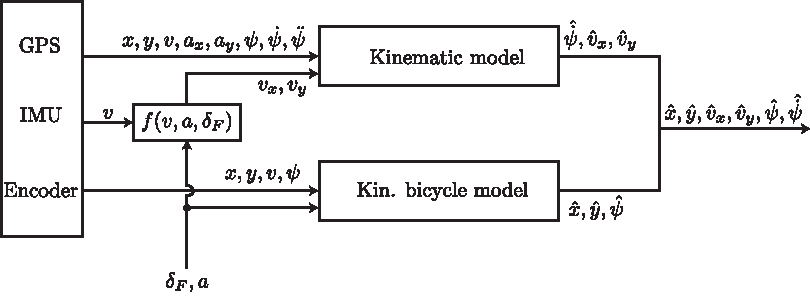
\includegraphics{../../Figures/Illustrator/FilterModel.pdf}
    \caption{Filter model}
    \label{fig:filter_model}
\end{figure}
This filtering approach is based on the assumption that only the kinematic bicycle model is able to estimate the current heading angle $\hat\psi$ using measurements of coordinates and velocity, while the kinematic model would not be able to account for the drift in the $\psi$ measurement. This is why the kinematic bicycle model is used to calculate the heading angle as well as the inertial coordinates. On the other hand, the kinematic model is well suited to combine measurements of accelerations, velocities, and position, which is why we use this model for the estimation of the yaw rate and velocities.

\subsection{Extended Kalman Filter}
Kalman filters provide a general tool to calculate a state estimate using noisy and/or biased sensor measurements assuming a gaussian model for the noise. The standard Kalman filter uses a linear model of the system in order to calculate the most probable state from a set of different state measurements.\\
Following general procedure has been taken from \cite{Bar-Shalom}.
The extended Kalman filter is based on the same principles as the standard Kalman filter but it allows to use a nonlinear model by linearizing the model at each time step.\\
The state estimation always consists of two steps: The \emph{Prediction step} and the \emph{Update step}. The first step calculates a prediction of the next state $\hat{\bm{x}}_{k|k-1}$ based on the previous state estimate $\hat{\bm{x}}_{k-1|k-1}$ and the control input $\bm{u}_{k-1}$. The update step corrects this prediction with the new measurement $\bm{z}_k$. The final state estimate is calculated using the Kalman gain $\bm{K}_k$. Both the model and measurement equations are linearized in each step.\\
Prediction:
\begin{align}
\hat{\bm{x}}_{k|k-1} &= f(\hat{\bm{x}}_{k-1|k-1},\bm{u}_{k-1})\\
\bm{P}_{k|k-1} &= \bm{F}_{k-1} \bm{P}_{k-1|k-1} \bm{F}_{k-1}^T + \bm{Q}_{k-1}
\end{align}
Update:
\begin{align}
\tilde{\bm{y}}_k &= \bm{z}_k - h(\hat{\bm{x}}_{k|k-1})\\
\bm{S}_k &= \bm{H}_k \bm{P}_{k|k-1} \bm{H}_k^T + \bm{R}_k\\
\bm{K}_k &= \bm{P}_{k|k-1}\bm{H}_k^T \bm{S}_k^{-1}\\
\hat{\bm{x}}_{k|k} &= \hat{\bm{x}}_{k|k-1} + \bm{K}_k \tilde{\bm{y}}_k\\
\bm{P}_{k|k} &= (\bm{I}-\bm{K}_k \bm{H}_k)\bm{P}_{k|k-1}
\end{align}

The predicted and updated estimate covariance $\bm{P}_{k|k-1}$ and $\bm{P}_{k|k}$, respectively, is a measure for the uncertainty of the state estimate. The process noise matrix $\bm{Q}$ is a measure for the uncertainty of the model, it is usually determined in experiments. The measurement noise matrix $\bm{R}$ depends on the noise values of the sensors. They are often provided in sensor data sheets or can otherwise be measured in experiments. The state transition and observation matrices $\bm F_k$ and $\bm{H}_k$ are the linearized functions $f(\bm{x},\bm{u})$ and $h(\bm{x})$:
\begin{align}
\bm{F}_k &= \left. \frac{\partial f}{\partial \bm{x}} \right|_{\hat{\bm{x}}_{k|k},\bm{u}_k}\\
\bm{H}_k &= \left. \frac{\partial h}{\partial \bm{x}} \right|_{\hat{\bm{x}}_{k|k-1}}
\end{align}
\subsection{Filter model}
The first filter features a kinematic bicycle model, eq. \eqref{eq:kinKalman} shows its model equations:
\begin{align}
\begin{split}\label{eq:kinKalman}
    \dot x &= v \cdot \cos (\psi + \beta)\\
    \dot y &= v \cdot \sin (\psi + \beta)\\
    \dot \psi &= \frac{v}{L_R}\cdot\sin(\beta)\\
    \dot v &= a - c_M\cdot v\\
    \dot d_\psi &= 0
\end{split}
\end{align}
with heading drift $d_\psi$.
There are two physical parameters, the first one is the distance $L_R$ between the rear axle and the GPS sensor which is measured as $L_R=\SI{0.125}{\meter}$. The second is the motor drag $c_M$ which was estimated in section \ref{sec:inputMapping} as $c_M=0.5$.\\
The measurement vector contains GPS, Encoder and heading measurements:
\begin{equation}
\bm{z} = \begin{pmatrix}
x_m&y_m&\psi_m&v_m
\end{pmatrix}^T,
\end{equation}
where the subscript $m$ denotes measured values. This leads to following measurement model:
\begin{equation}
h(\hat{\bm{x}}_{k|k-1}) = \begin{pmatrix}
1 & 0 & 0 & 0 & 0\\
0 & 1 & 0 & 0 & 0\\
0 & 0 & 1 & 0 & 1\\
0 & 0 & 0 & 1 & 0
\end{pmatrix} \hat{\bm{x}}_{k|k-1}=
\begin{pmatrix}
\hat x\\
\hat y\\
\hat \psi + \hat d_\psi\\
\hat v
\end{pmatrix}
\end{equation} 
The second filter features a pure kinematic motion model from \cite{Caron2006} which integrates accelerations to find velocities and positions.
%{\bfseries{Why do you use position from the other model and not from this one, as shown in Figure 4.6. --> mb: I ran experiments comparing the x-y-estimates from both estimators and the kin-model estimates proved to be better ("better" meaning closer to the raw GPS data.)}}.
Eq. \eqref{eq:dynKalman} shows its model equations:
\begin{align}
\begin{split}\label{eq:dynKalman}
    \dot x &= \cos(\psi) v_x - \sin(\psi) v_y\\
    \dot y &= \sin(\psi) v_x + \cos(\psi) v_y\\
    \dot v_x &= a_x + \dot \psi v_y\\
    \dot v_y &= a_y - \dot \psi v_x\\
    \dot \psi &= \dot \psi\\
    \ddot \psi  &= 0\\
    \dot a_x &= 0\\
    \dot a_y &= 0\\
    \dot d_\psi &= 0
\end{split}
\end{align}
It uses the longitudinal and angular acceleration measurements of the IMU and position measurements of the GPS. Since the car's suspension leads to strong tilting motions in curves, the measurements of $a_y$ are distorted significantly. In order to support a correct estimation of $v_y$ and to reduce the effect of drift errors in $a_y$, the system additionally receives artificial measurements of $v_x$ and $v_y$. These are constructed by following relations:
\begin{align*}
v_{x,m} &= v_m\cos(\delta_F)\\
v_{y,m} &= v_m\sin(\delta_F)
\end{align*}
where $v$ is the encoder measurement and $\delta_F$ the control input.
Thus, the measurement vector of the second filter uses following measurements:
\begin{equation}
\bm{z}=\begin{pmatrix}x_m&y_m&v_{x,m}&v_{y,m}&\psi_m&\dot\psi_m&\ddot\psi_m&a_{x,m}&a_{y,m}\end{pmatrix}^T
\end{equation}
% Tuning of Q and R matrices
\paragraph{Tuning of Q and R matrices}
The measurement noise matrices were constructed assuming diagonal matrices (independent sensors) and measuring the sensor noises during operation.\\
The process noise matrix Q was tuned manually in post-processing. The values were tuned with the objective to provide a smooth fit to the raw measurements.
\paragraph{Frequency of the filter}
The extended Kalman filter runs at a frequency of 50 Hertz and assumes that all measurements are received at the same time and with equal frequencies. However, since we are using different sensors at different frequencies, we are using following strategy for each sensor:
\begin{description}
\item[IMU] The IMU provides data at the frequency of the Kalman filter itself, $\SI{50}{\hertz}$. This is why we can use this data directly.
\item[GPS] The indoor GPS provides measurements at varying frequencies between 10 and 16 Hertz, whereas there are times when no measurement are received for up to one second. These interruptions might result from hardware issues (e.g. interfering reflections of ultrasound, timing issues) and could not be resolved. In order to account for this uncertainty, we always extrapolate the previously received data by  polynomials to the timestamp of the Kalman filter update. This extrapolation makes sure that even longer measurement breaks don't pose any difficulties to the estimator.
\item[Encoder] Three of the car's wheels are equipped with encoders, using 2 magnets each. The frequency of signals from these encoders can be calculated as follows:
\begin{equation}
f =\frac{1}{T}=\frac{v}{\pi r}
\end{equation}
with the velocity $v$ and the wheel radius $r$. This means that at a velocity of $\SI{1.0}{\meter\per\second}$ and for a wheel radius of $\SI{3.6}{\centi\meter}$, we receive a velocity measurement from each wheel at a rate of about $\SI{9}{\hertz}$. These measurements are not synchronized as the wheels start at different angles. All measurements are received by the arduino, averaged, and then sent to the filter at a constant rate of $\SI{50}{\hertz}$. Since even with three encoders we can't reach a real update rate of $\SI{50}{\hertz}$, we assume a rather high encoder measurement noise in the measurement noise matrix $\bm{R}$ to account for equal consecutive measurements.
\end{description}
\subsection{Mapping to the track reference frame}
The estimator discussed above returns a state estimate in the inertial frame which then needs to be transformed into the track reference frame. The coordinates in the track reference frame are the curvilinear abscissa $s$, the lateral position error $e_Y$, and the heading error $e_\psi$. The procedure for this transformation is described below.\\
We assume that the track is given by $n$ equidistant vertices with coordinates $\bm{x}_i = \begin{pmatrix}
x_i&y_i
\end{pmatrix},i=1...n$.

\begin{enumerate}
\item Find the closest vertex $\bm{x}_i$ of the track to the current position of the car
\item Select a set of vertices around vertex $i$
\item Use this set to approximate the track locally using a polynomial, returning functions for the coordinates $(x,y)=f(s)$ and curvature $c=f(s)$
\item Use these functions to calculate the current curvilinear abscissa $s$, lateral position $e_Y$ and heading error $e_\psi$.
\end{enumerate}
The number of points used for the approximation and the polynomial degree have to be chosen in such a way to provide an accurate fit throughout the entire prediction horizon.\\
In practice, we used a polynomial of 8\textsuperscript{th} degree. This polynomial proved to approximate the piecewise linear curvature well enough while keeping the complexity of the optimization problem at a reasonable level.
%The procedure is shown in fig. \ref{fig:s_ey_poly}.
%\begin{figure}[ht]
%    \centering
%      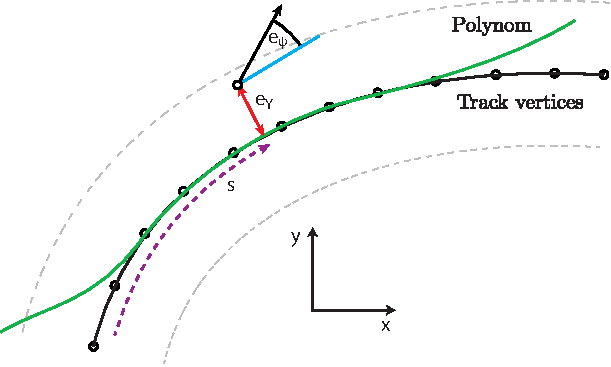
\includegraphics{../../Figures/Mapping/s_ey.pdf}
%    \caption{$s-e_Y-$frame}
%    \label{fig:s_ey_poly}
%\end{figure}

\section{System Identification}\label{sec:sysID}
In order to provide an accurate model to the MPC, the system's dynamics are identified at each time step. The dynamic bicycle model from eq. \eqref{eq:dynModel} is used to derive a Linear Regression model that uses functions of the system's states as features. State estimates from previous laps are then used to calculate current parameters $\theta_{i,j}$.

Linear Regression model of the dynamic bicycle model:
\begin{align}
    v_{x,k+1} - v_{x,k}&= \theta_{x,1} \cdot v_{y,k} \cdot \dot\psi_k + \theta_{x,2}\cdot v_{x,k}  + \theta_{x,3}\cdot a_k\\
    v_{y,k+1}- v_{y,k} &= \theta_{y,1}\cdot  \frac{v_{y,k}}{v_{x,k}}+\theta_{y,2}\cdot v_{x,k}\dot\psi_k + \theta_{y,3}\cdot \frac{\dot\psi_k}{v_{x,k}}+\theta_{y,4}\cdot \delta_k\\
    \dot\psi_{k+1}-\dot\psi_k &= \theta_{\psi,1}\cdot \frac{\dot\psi_k}{v_{x,k}}+\theta_{\psi,2}\cdot \frac{v_{y,k}}{v_{x,k}}+\theta_{\psi,3}\cdot \delta_k
\end{align}
with states $v_x$, $v_y$, $\dot \psi$ and parameters $\theta_{i,j}$. The features $\bm{X}$ of this Linear Regression problem are functions of the states and inputs. Using multiple samples $n$, each equation can be rewritten as
\begin{equation}
\bm{y}=\bm{X\theta}.
\end{equation}
Equation \eqref{eq:LRvx} shows the equations for the LR of $v_x$:
\begin{align}
\label{eq:LRvx}
\bm{y} = \begin{pmatrix}
v_{x,2} - v_{x,1}\\
v_{x,3} - v_{x,2}\\
\vdots\\
v_{x,n} - v_{x,n-1}
\end{pmatrix} &&
\bm{X} = \begin{pmatrix}
v_{y,1} & \dot\psi_{1} & a_{1}\\
v_{y,2} & \dot\psi_{2} & a_{2}\\
\vdots\\
v_{y,n-1} & \dot\psi_{n-1} & a_{n-1}
\end{pmatrix}&&
\bm{\theta}=\begin{pmatrix}
\theta_{x,1}\\
\theta_{x,2}\\
\theta_{x,3}
\end{pmatrix}
\end{align}
The LR equations for $v_y$ and $\dot\psi$ can be writte n in the same way.\\
To determine the optimal parameters $\bm{\theta}^*$, following minimization has to be solved:
\begin{equation}
\bm{\theta}^* = \argmin_{\bm{\theta}} \| \bm{X\theta}-\bm{y} \|_2
\end{equation}
There are different approaches to solve this problem, in this case the \emph{normal equation} method is used. This leads to following analytic solution:
\begin{equation}
\bm{\theta}^* = (\bm{X}^T \bm{X})^{-1}\bm{X}^T \bm{y}
\end{equation}
Since we are using about $n=100...1000$ samples, the calculation of the inverse of $\bm{X}^T \bm{X}$ is still sufficiently fast. However, if we were to use even more samples, other methods such as \emph{gradient descent} might work faster.

\section{Implementation}\label{sec:implementation}
The estimator and MPC solver are implemented in the ROS framework (Robot Operating System, \cite{ros}). The sensor data is sent from the BARC to a more powerful CPU (Macbook Pro 2010, 2.4 GHz) which solves the MPC problem at a rate of 10 Hertz and sends the optimal input to the BARC. The setup is illustrated in fig. \ref{fig:architecture}.
\begin{figure}[ht]
    \centering
      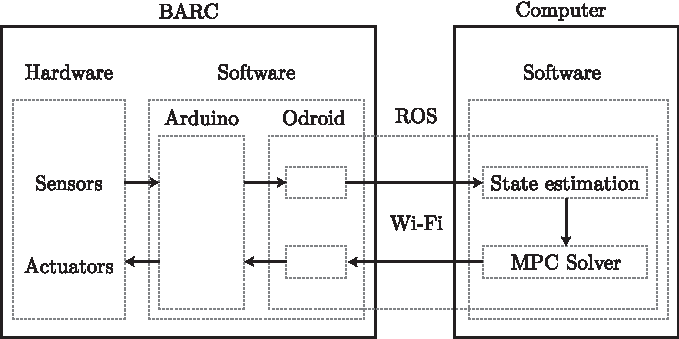
\includegraphics{../../Figures/Illustrator/Architecture.pdf}
    \caption{Software/Hardware setup}
    \label{fig:architecture}
\end{figure}
The ROS framework manages the execution of all scripts and makes sure that they are running at their specified frequencies. It also manages the wireless communication between the odroid and the computer.\\
The estimator is a python script that runs at a constant frequency of $\SI{50}{\hertz}$, which is the highest frequency at which measurements are received by the IMU. Both the encoders and the GPS are running at lower or variable frequencies between 10 and $\SI{50}{\hertz}$.\\
The MPC optimization problem is solved by Ipopt \cite{ipopt} which is executed by a script written in Julia 0.4.6 \cite{julia}. It solves the LMPC problem at a constant frequency of $\SI{10}{\hertz}$ and sends the optimal control input to the BARC. At the same time, it receives and saves all state estimates from the estimator.\\
Since we need to maintain a constant input rate of $\SI{10}{\hertz}$ while the optimization process can last different times (at most $\SI{0.1}{\second}$), the commands are always sent at the beginning of one time step. The MPC solver uses an initial state that is predicted by 0.1 seconds from the most recent estimated state. Figure \ref{fig:timing} shows the timing diagram of ROS nodes and messages.
\begin{figure}[ht]
    \centering
\begin{wave}{4}{2}
\nextwave{Estimator} \known{}{0.05}\unknown[]{0.15}
                \known{}{0.07}\unknown[]{0.13}
                \known{}{0.04}\unknown[]{0.16}
                \known{}{0.06}\unknown[]{0.14}
                \known{}{0.08}\unknown[]{0.12}
                \known{}{0.09}\unknown[]{0.11}
                \known{}{0.06}\unknown[]{0.14}
                \known{}{0.05}\unknown[]{0.15}
                \known{}{0.09}\unknown[]{0.11}
                \known{}{0.04}\unknown[]{0.16}
                \known{}{0.03}\unknown[]{0.17}
                \known{}{0.07}\unknown[]{0.13}
                \known{}{0.08}\unknown[]{0.12}
                \known{}{0.06}\unknown[]{0.14}
                \known{}{0.07}\unknown[]{0.13}
\nextwave{MPC} \known{MPC}{0.7}\unknown[]{0.3}\known{MPC}{0.5}\unknown[]{0.5}\known{MPC}{0.8}\unknown[]{0.2}
\nextwave{Command} \known{}{0.05}\unknown[]{0.95}
                \known{}{0.05}\unknown[]{0.95}
                \known{}{0.05}\unknown[]{0.95}

\end{wave}
\caption{Timing diagram}
    \label{fig:timing}
\end{figure}

Below are described all steps that are performed during one time step (asynchronously). Additionally, figure \ref{fig:controlStructure} illustrates the closed-loop system.
\begin{enumerate}
\item State estimation
\begin{enumerate}
\item Read sensor data
\item Calculate the current state in the inertial frame
\item Transform the state to the track frame
\item Calculate polynomial coefficients that approximate the curvature locally
\end{enumerate}
\item System Identification
\begin{enumerate}
\item Select data from previous and current lap
\item Calculate Matrices of features
\item Calculate parameters of system dynamics using Linear Regression
\end{enumerate}
\item Approximate safe set and cost function
\begin{enumerate}
\item Select locally near data from previous laps
\item Calculate polynomials that approximate this data to construct the safe set
\end{enumerate}
\item Solve the LMPC problem
\begin{enumerate}
\item Use the state estimate as initial state for the MPC formulation
\item Minimize the cost function, using state dynamics from the Linear Regression and curvature as well as the safe set and terminal cost function
\item Send the optimal input to the actuators
\end{enumerate}
\end{enumerate}

\begin{figure}[ht]
    \centering
  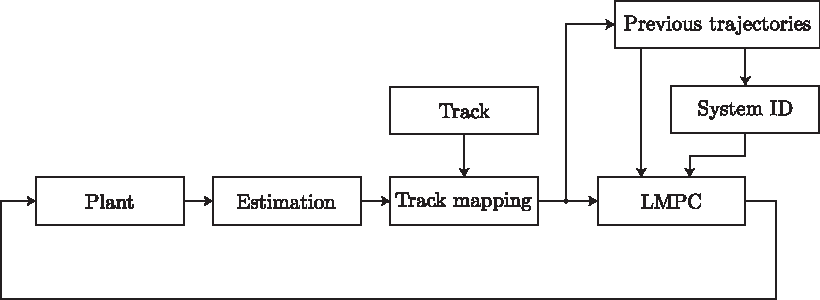
\includegraphics{../../Figures/Illustrator/ControlDiagram.pdf}
    \caption{Control structure}
    \label{fig:controlStructure}
\end{figure}

\section{Experiments}
%{\bfseries{Made a new Chapter for experimental results}} 
The experiments were performed in a closed space at UC Berkeley. The available area had a size of about 5 by 8 meters and provided enough space for a simple race track.\\
We chose a race track that fits the available area while still providing turns in different directions with the maximum possible curvature of $\SI{1.24}{\per\meter}$. The curvature is shown in fig. \ref{fig:exp_curv}. The track length is $\SI{19}{\meter}$.
We used a constant sample size for the system identification of 120 points per lap which corresponds to $\SI{2.4}{\second}$ since the state estimation runs at $\SI{50}{\hertz}$. We also used an LMPC horizon length of $N=12$ which corresponds to a prediction time of $\SI{1.2}{\second}$. This horizon is a trade-off between fast learning and fast solver times.
\begin{figure}[ht]
    \centering
      %% Creator: Matplotlib, PGF backend
%%
%% To include the figure in your LaTeX document, write
%%   \input{<filename>.pgf}
%%
%% Make sure the required packages are loaded in your preamble
%%   \usepackage{pgf}
%%
%% Figures using additional raster images can only be included by \input if
%% they are in the same directory as the main LaTeX file. For loading figures
%% from other directories you can use the `import` package
%%   \usepackage{import}
%% and then include the figures with
%%   \import{<path to file>}{<filename>.pgf}
%%
%% Matplotlib used the following preamble
%%   \usepackage{fontspec}
%%
\begingroup%
\makeatletter%
\begin{pgfpicture}%
\pgfpathrectangle{\pgfpointorigin}{\pgfqpoint{4.500000in}{3.000000in}}%
\pgfusepath{use as bounding box, clip}%
\begin{pgfscope}%
\pgfsetbuttcap%
\pgfsetmiterjoin%
\definecolor{currentfill}{rgb}{1.000000,1.000000,1.000000}%
\pgfsetfillcolor{currentfill}%
\pgfsetlinewidth{0.000000pt}%
\definecolor{currentstroke}{rgb}{1.000000,1.000000,1.000000}%
\pgfsetstrokecolor{currentstroke}%
\pgfsetdash{}{0pt}%
\pgfpathmoveto{\pgfqpoint{0.000000in}{0.000000in}}%
\pgfpathlineto{\pgfqpoint{4.500000in}{0.000000in}}%
\pgfpathlineto{\pgfqpoint{4.500000in}{3.000000in}}%
\pgfpathlineto{\pgfqpoint{0.000000in}{3.000000in}}%
\pgfpathclose%
\pgfusepath{fill}%
\end{pgfscope}%
\begin{pgfscope}%
\pgfsetbuttcap%
\pgfsetmiterjoin%
\definecolor{currentfill}{rgb}{1.000000,1.000000,1.000000}%
\pgfsetfillcolor{currentfill}%
\pgfsetlinewidth{0.000000pt}%
\definecolor{currentstroke}{rgb}{0.000000,0.000000,0.000000}%
\pgfsetstrokecolor{currentstroke}%
\pgfsetstrokeopacity{0.000000}%
\pgfsetdash{}{0pt}%
\pgfpathmoveto{\pgfqpoint{0.628958in}{0.471921in}}%
\pgfpathlineto{\pgfqpoint{4.291316in}{0.471921in}}%
\pgfpathlineto{\pgfqpoint{4.291316in}{2.805251in}}%
\pgfpathlineto{\pgfqpoint{0.628958in}{2.805251in}}%
\pgfpathclose%
\pgfusepath{fill}%
\end{pgfscope}%
\begin{pgfscope}%
\pgfpathrectangle{\pgfqpoint{0.628958in}{0.471921in}}{\pgfqpoint{3.662359in}{2.333330in}} %
\pgfusepath{clip}%
\pgfsetrectcap%
\pgfsetroundjoin%
\pgfsetlinewidth{0.501875pt}%
\definecolor{currentstroke}{rgb}{0.000000,0.000000,1.000000}%
\pgfsetstrokecolor{currentstroke}%
\pgfsetdash{}{0pt}%
\pgfpathmoveto{\pgfqpoint{0.630789in}{1.871919in}}%
\pgfpathlineto{\pgfqpoint{0.960401in}{1.871919in}}%
\pgfpathlineto{\pgfqpoint{1.169156in}{0.650190in}}%
\pgfpathlineto{\pgfqpoint{1.180143in}{0.650190in}}%
\pgfpathlineto{\pgfqpoint{1.388897in}{1.871919in}}%
\pgfpathlineto{\pgfqpoint{1.509755in}{1.871919in}}%
\pgfpathlineto{\pgfqpoint{1.718509in}{0.650190in}}%
\pgfpathlineto{\pgfqpoint{1.729496in}{0.650190in}}%
\pgfpathlineto{\pgfqpoint{1.938251in}{1.871919in}}%
\pgfpathlineto{\pgfqpoint{1.949238in}{1.871919in}}%
\pgfpathlineto{\pgfqpoint{2.048122in}{2.360611in}}%
\pgfpathlineto{\pgfqpoint{2.059109in}{2.360611in}}%
\pgfpathlineto{\pgfqpoint{2.157992in}{1.871919in}}%
\pgfpathlineto{\pgfqpoint{2.168980in}{1.871919in}}%
\pgfpathlineto{\pgfqpoint{2.322799in}{1.220330in}}%
\pgfpathlineto{\pgfqpoint{2.333786in}{1.220330in}}%
\pgfpathlineto{\pgfqpoint{2.487605in}{1.871919in}}%
\pgfpathlineto{\pgfqpoint{2.498592in}{1.871919in}}%
\pgfpathlineto{\pgfqpoint{2.597476in}{2.360611in}}%
\pgfpathlineto{\pgfqpoint{2.608463in}{2.360611in}}%
\pgfpathlineto{\pgfqpoint{2.707346in}{1.871919in}}%
\pgfpathlineto{\pgfqpoint{2.718333in}{1.871919in}}%
\pgfpathlineto{\pgfqpoint{2.927088in}{0.650190in}}%
\pgfpathlineto{\pgfqpoint{2.938075in}{0.650190in}}%
\pgfpathlineto{\pgfqpoint{3.146829in}{1.871919in}}%
\pgfpathlineto{\pgfqpoint{3.267687in}{1.871919in}}%
\pgfpathlineto{\pgfqpoint{3.476442in}{0.650190in}}%
\pgfpathlineto{\pgfqpoint{3.487429in}{0.650190in}}%
\pgfpathlineto{\pgfqpoint{3.696183in}{1.871919in}}%
\pgfpathlineto{\pgfqpoint{4.080731in}{1.871919in}}%
\pgfpathlineto{\pgfqpoint{4.080731in}{1.871919in}}%
\pgfusepath{stroke}%
\end{pgfscope}%
\begin{pgfscope}%
\pgfsetrectcap%
\pgfsetmiterjoin%
\pgfsetlinewidth{0.501875pt}%
\definecolor{currentstroke}{rgb}{0.000000,0.000000,0.000000}%
\pgfsetstrokecolor{currentstroke}%
\pgfsetdash{}{0pt}%
\pgfpathmoveto{\pgfqpoint{0.628958in}{2.805251in}}%
\pgfpathlineto{\pgfqpoint{4.291316in}{2.805251in}}%
\pgfusepath{stroke}%
\end{pgfscope}%
\begin{pgfscope}%
\pgfsetrectcap%
\pgfsetmiterjoin%
\pgfsetlinewidth{0.501875pt}%
\definecolor{currentstroke}{rgb}{0.000000,0.000000,0.000000}%
\pgfsetstrokecolor{currentstroke}%
\pgfsetdash{}{0pt}%
\pgfpathmoveto{\pgfqpoint{4.291316in}{0.471921in}}%
\pgfpathlineto{\pgfqpoint{4.291316in}{2.805251in}}%
\pgfusepath{stroke}%
\end{pgfscope}%
\begin{pgfscope}%
\pgfsetrectcap%
\pgfsetmiterjoin%
\pgfsetlinewidth{0.501875pt}%
\definecolor{currentstroke}{rgb}{0.000000,0.000000,0.000000}%
\pgfsetstrokecolor{currentstroke}%
\pgfsetdash{}{0pt}%
\pgfpathmoveto{\pgfqpoint{0.628958in}{0.471921in}}%
\pgfpathlineto{\pgfqpoint{4.291316in}{0.471921in}}%
\pgfusepath{stroke}%
\end{pgfscope}%
\begin{pgfscope}%
\pgfsetrectcap%
\pgfsetmiterjoin%
\pgfsetlinewidth{0.501875pt}%
\definecolor{currentstroke}{rgb}{0.000000,0.000000,0.000000}%
\pgfsetstrokecolor{currentstroke}%
\pgfsetdash{}{0pt}%
\pgfpathmoveto{\pgfqpoint{0.628958in}{0.471921in}}%
\pgfpathlineto{\pgfqpoint{0.628958in}{2.805251in}}%
\pgfusepath{stroke}%
\end{pgfscope}%
\begin{pgfscope}%
\pgfpathrectangle{\pgfqpoint{0.628958in}{0.471921in}}{\pgfqpoint{3.662359in}{2.333330in}} %
\pgfusepath{clip}%
\pgfsetbuttcap%
\pgfsetroundjoin%
\pgfsetlinewidth{0.501875pt}%
\definecolor{currentstroke}{rgb}{0.000000,0.000000,0.000000}%
\pgfsetstrokecolor{currentstroke}%
\pgfsetdash{{1.000000pt}{3.000000pt}}{0.000000pt}%
\pgfpathmoveto{\pgfqpoint{0.628958in}{0.471921in}}%
\pgfpathlineto{\pgfqpoint{0.628958in}{2.805251in}}%
\pgfusepath{stroke}%
\end{pgfscope}%
\begin{pgfscope}%
\pgfsetbuttcap%
\pgfsetroundjoin%
\definecolor{currentfill}{rgb}{0.000000,0.000000,0.000000}%
\pgfsetfillcolor{currentfill}%
\pgfsetlinewidth{0.250937pt}%
\definecolor{currentstroke}{rgb}{0.000000,0.000000,0.000000}%
\pgfsetstrokecolor{currentstroke}%
\pgfsetdash{}{0pt}%
\pgfsys@defobject{currentmarker}{\pgfqpoint{0.000000in}{0.000000in}}{\pgfqpoint{0.000000in}{0.055556in}}{%
\pgfpathmoveto{\pgfqpoint{0.000000in}{0.000000in}}%
\pgfpathlineto{\pgfqpoint{0.000000in}{0.055556in}}%
\pgfusepath{stroke,fill}%
}%
\begin{pgfscope}%
\pgfsys@transformshift{0.628958in}{0.471921in}%
\pgfsys@useobject{currentmarker}{}%
\end{pgfscope}%
\end{pgfscope}%
\begin{pgfscope}%
\pgfsetbuttcap%
\pgfsetroundjoin%
\definecolor{currentfill}{rgb}{0.000000,0.000000,0.000000}%
\pgfsetfillcolor{currentfill}%
\pgfsetlinewidth{0.250937pt}%
\definecolor{currentstroke}{rgb}{0.000000,0.000000,0.000000}%
\pgfsetstrokecolor{currentstroke}%
\pgfsetdash{}{0pt}%
\pgfsys@defobject{currentmarker}{\pgfqpoint{0.000000in}{-0.055556in}}{\pgfqpoint{0.000000in}{0.000000in}}{%
\pgfpathmoveto{\pgfqpoint{0.000000in}{0.000000in}}%
\pgfpathlineto{\pgfqpoint{0.000000in}{-0.055556in}}%
\pgfusepath{stroke,fill}%
}%
\begin{pgfscope}%
\pgfsys@transformshift{0.628958in}{2.805251in}%
\pgfsys@useobject{currentmarker}{}%
\end{pgfscope}%
\end{pgfscope}%
\begin{pgfscope}%
\pgftext[x=0.628958in,y=0.416365in,,top]{\rmfamily\fontsize{6.940000}{8.328000}\selectfont \(\displaystyle 0\)}%
\end{pgfscope}%
\begin{pgfscope}%
\pgfpathrectangle{\pgfqpoint{0.628958in}{0.471921in}}{\pgfqpoint{3.662359in}{2.333330in}} %
\pgfusepath{clip}%
\pgfsetbuttcap%
\pgfsetroundjoin%
\pgfsetlinewidth{0.501875pt}%
\definecolor{currentstroke}{rgb}{0.000000,0.000000,0.000000}%
\pgfsetstrokecolor{currentstroke}%
\pgfsetdash{{1.000000pt}{3.000000pt}}{0.000000pt}%
\pgfpathmoveto{\pgfqpoint{1.544547in}{0.471921in}}%
\pgfpathlineto{\pgfqpoint{1.544547in}{2.805251in}}%
\pgfusepath{stroke}%
\end{pgfscope}%
\begin{pgfscope}%
\pgfsetbuttcap%
\pgfsetroundjoin%
\definecolor{currentfill}{rgb}{0.000000,0.000000,0.000000}%
\pgfsetfillcolor{currentfill}%
\pgfsetlinewidth{0.250937pt}%
\definecolor{currentstroke}{rgb}{0.000000,0.000000,0.000000}%
\pgfsetstrokecolor{currentstroke}%
\pgfsetdash{}{0pt}%
\pgfsys@defobject{currentmarker}{\pgfqpoint{0.000000in}{0.000000in}}{\pgfqpoint{0.000000in}{0.055556in}}{%
\pgfpathmoveto{\pgfqpoint{0.000000in}{0.000000in}}%
\pgfpathlineto{\pgfqpoint{0.000000in}{0.055556in}}%
\pgfusepath{stroke,fill}%
}%
\begin{pgfscope}%
\pgfsys@transformshift{1.544547in}{0.471921in}%
\pgfsys@useobject{currentmarker}{}%
\end{pgfscope}%
\end{pgfscope}%
\begin{pgfscope}%
\pgfsetbuttcap%
\pgfsetroundjoin%
\definecolor{currentfill}{rgb}{0.000000,0.000000,0.000000}%
\pgfsetfillcolor{currentfill}%
\pgfsetlinewidth{0.250937pt}%
\definecolor{currentstroke}{rgb}{0.000000,0.000000,0.000000}%
\pgfsetstrokecolor{currentstroke}%
\pgfsetdash{}{0pt}%
\pgfsys@defobject{currentmarker}{\pgfqpoint{0.000000in}{-0.055556in}}{\pgfqpoint{0.000000in}{0.000000in}}{%
\pgfpathmoveto{\pgfqpoint{0.000000in}{0.000000in}}%
\pgfpathlineto{\pgfqpoint{0.000000in}{-0.055556in}}%
\pgfusepath{stroke,fill}%
}%
\begin{pgfscope}%
\pgfsys@transformshift{1.544547in}{2.805251in}%
\pgfsys@useobject{currentmarker}{}%
\end{pgfscope}%
\end{pgfscope}%
\begin{pgfscope}%
\pgftext[x=1.544547in,y=0.416365in,,top]{\rmfamily\fontsize{6.940000}{8.328000}\selectfont \(\displaystyle 5\)}%
\end{pgfscope}%
\begin{pgfscope}%
\pgfpathrectangle{\pgfqpoint{0.628958in}{0.471921in}}{\pgfqpoint{3.662359in}{2.333330in}} %
\pgfusepath{clip}%
\pgfsetbuttcap%
\pgfsetroundjoin%
\pgfsetlinewidth{0.501875pt}%
\definecolor{currentstroke}{rgb}{0.000000,0.000000,0.000000}%
\pgfsetstrokecolor{currentstroke}%
\pgfsetdash{{1.000000pt}{3.000000pt}}{0.000000pt}%
\pgfpathmoveto{\pgfqpoint{2.460137in}{0.471921in}}%
\pgfpathlineto{\pgfqpoint{2.460137in}{2.805251in}}%
\pgfusepath{stroke}%
\end{pgfscope}%
\begin{pgfscope}%
\pgfsetbuttcap%
\pgfsetroundjoin%
\definecolor{currentfill}{rgb}{0.000000,0.000000,0.000000}%
\pgfsetfillcolor{currentfill}%
\pgfsetlinewidth{0.250937pt}%
\definecolor{currentstroke}{rgb}{0.000000,0.000000,0.000000}%
\pgfsetstrokecolor{currentstroke}%
\pgfsetdash{}{0pt}%
\pgfsys@defobject{currentmarker}{\pgfqpoint{0.000000in}{0.000000in}}{\pgfqpoint{0.000000in}{0.055556in}}{%
\pgfpathmoveto{\pgfqpoint{0.000000in}{0.000000in}}%
\pgfpathlineto{\pgfqpoint{0.000000in}{0.055556in}}%
\pgfusepath{stroke,fill}%
}%
\begin{pgfscope}%
\pgfsys@transformshift{2.460137in}{0.471921in}%
\pgfsys@useobject{currentmarker}{}%
\end{pgfscope}%
\end{pgfscope}%
\begin{pgfscope}%
\pgfsetbuttcap%
\pgfsetroundjoin%
\definecolor{currentfill}{rgb}{0.000000,0.000000,0.000000}%
\pgfsetfillcolor{currentfill}%
\pgfsetlinewidth{0.250937pt}%
\definecolor{currentstroke}{rgb}{0.000000,0.000000,0.000000}%
\pgfsetstrokecolor{currentstroke}%
\pgfsetdash{}{0pt}%
\pgfsys@defobject{currentmarker}{\pgfqpoint{0.000000in}{-0.055556in}}{\pgfqpoint{0.000000in}{0.000000in}}{%
\pgfpathmoveto{\pgfqpoint{0.000000in}{0.000000in}}%
\pgfpathlineto{\pgfqpoint{0.000000in}{-0.055556in}}%
\pgfusepath{stroke,fill}%
}%
\begin{pgfscope}%
\pgfsys@transformshift{2.460137in}{2.805251in}%
\pgfsys@useobject{currentmarker}{}%
\end{pgfscope}%
\end{pgfscope}%
\begin{pgfscope}%
\pgftext[x=2.460137in,y=0.416365in,,top]{\rmfamily\fontsize{6.940000}{8.328000}\selectfont \(\displaystyle 10\)}%
\end{pgfscope}%
\begin{pgfscope}%
\pgfpathrectangle{\pgfqpoint{0.628958in}{0.471921in}}{\pgfqpoint{3.662359in}{2.333330in}} %
\pgfusepath{clip}%
\pgfsetbuttcap%
\pgfsetroundjoin%
\pgfsetlinewidth{0.501875pt}%
\definecolor{currentstroke}{rgb}{0.000000,0.000000,0.000000}%
\pgfsetstrokecolor{currentstroke}%
\pgfsetdash{{1.000000pt}{3.000000pt}}{0.000000pt}%
\pgfpathmoveto{\pgfqpoint{3.375727in}{0.471921in}}%
\pgfpathlineto{\pgfqpoint{3.375727in}{2.805251in}}%
\pgfusepath{stroke}%
\end{pgfscope}%
\begin{pgfscope}%
\pgfsetbuttcap%
\pgfsetroundjoin%
\definecolor{currentfill}{rgb}{0.000000,0.000000,0.000000}%
\pgfsetfillcolor{currentfill}%
\pgfsetlinewidth{0.250937pt}%
\definecolor{currentstroke}{rgb}{0.000000,0.000000,0.000000}%
\pgfsetstrokecolor{currentstroke}%
\pgfsetdash{}{0pt}%
\pgfsys@defobject{currentmarker}{\pgfqpoint{0.000000in}{0.000000in}}{\pgfqpoint{0.000000in}{0.055556in}}{%
\pgfpathmoveto{\pgfqpoint{0.000000in}{0.000000in}}%
\pgfpathlineto{\pgfqpoint{0.000000in}{0.055556in}}%
\pgfusepath{stroke,fill}%
}%
\begin{pgfscope}%
\pgfsys@transformshift{3.375727in}{0.471921in}%
\pgfsys@useobject{currentmarker}{}%
\end{pgfscope}%
\end{pgfscope}%
\begin{pgfscope}%
\pgfsetbuttcap%
\pgfsetroundjoin%
\definecolor{currentfill}{rgb}{0.000000,0.000000,0.000000}%
\pgfsetfillcolor{currentfill}%
\pgfsetlinewidth{0.250937pt}%
\definecolor{currentstroke}{rgb}{0.000000,0.000000,0.000000}%
\pgfsetstrokecolor{currentstroke}%
\pgfsetdash{}{0pt}%
\pgfsys@defobject{currentmarker}{\pgfqpoint{0.000000in}{-0.055556in}}{\pgfqpoint{0.000000in}{0.000000in}}{%
\pgfpathmoveto{\pgfqpoint{0.000000in}{0.000000in}}%
\pgfpathlineto{\pgfqpoint{0.000000in}{-0.055556in}}%
\pgfusepath{stroke,fill}%
}%
\begin{pgfscope}%
\pgfsys@transformshift{3.375727in}{2.805251in}%
\pgfsys@useobject{currentmarker}{}%
\end{pgfscope}%
\end{pgfscope}%
\begin{pgfscope}%
\pgftext[x=3.375727in,y=0.416365in,,top]{\rmfamily\fontsize{6.940000}{8.328000}\selectfont \(\displaystyle 15\)}%
\end{pgfscope}%
\begin{pgfscope}%
\pgfpathrectangle{\pgfqpoint{0.628958in}{0.471921in}}{\pgfqpoint{3.662359in}{2.333330in}} %
\pgfusepath{clip}%
\pgfsetbuttcap%
\pgfsetroundjoin%
\pgfsetlinewidth{0.501875pt}%
\definecolor{currentstroke}{rgb}{0.000000,0.000000,0.000000}%
\pgfsetstrokecolor{currentstroke}%
\pgfsetdash{{1.000000pt}{3.000000pt}}{0.000000pt}%
\pgfpathmoveto{\pgfqpoint{4.291316in}{0.471921in}}%
\pgfpathlineto{\pgfqpoint{4.291316in}{2.805251in}}%
\pgfusepath{stroke}%
\end{pgfscope}%
\begin{pgfscope}%
\pgfsetbuttcap%
\pgfsetroundjoin%
\definecolor{currentfill}{rgb}{0.000000,0.000000,0.000000}%
\pgfsetfillcolor{currentfill}%
\pgfsetlinewidth{0.250937pt}%
\definecolor{currentstroke}{rgb}{0.000000,0.000000,0.000000}%
\pgfsetstrokecolor{currentstroke}%
\pgfsetdash{}{0pt}%
\pgfsys@defobject{currentmarker}{\pgfqpoint{0.000000in}{0.000000in}}{\pgfqpoint{0.000000in}{0.055556in}}{%
\pgfpathmoveto{\pgfqpoint{0.000000in}{0.000000in}}%
\pgfpathlineto{\pgfqpoint{0.000000in}{0.055556in}}%
\pgfusepath{stroke,fill}%
}%
\begin{pgfscope}%
\pgfsys@transformshift{4.291316in}{0.471921in}%
\pgfsys@useobject{currentmarker}{}%
\end{pgfscope}%
\end{pgfscope}%
\begin{pgfscope}%
\pgfsetbuttcap%
\pgfsetroundjoin%
\definecolor{currentfill}{rgb}{0.000000,0.000000,0.000000}%
\pgfsetfillcolor{currentfill}%
\pgfsetlinewidth{0.250937pt}%
\definecolor{currentstroke}{rgb}{0.000000,0.000000,0.000000}%
\pgfsetstrokecolor{currentstroke}%
\pgfsetdash{}{0pt}%
\pgfsys@defobject{currentmarker}{\pgfqpoint{0.000000in}{-0.055556in}}{\pgfqpoint{0.000000in}{0.000000in}}{%
\pgfpathmoveto{\pgfqpoint{0.000000in}{0.000000in}}%
\pgfpathlineto{\pgfqpoint{0.000000in}{-0.055556in}}%
\pgfusepath{stroke,fill}%
}%
\begin{pgfscope}%
\pgfsys@transformshift{4.291316in}{2.805251in}%
\pgfsys@useobject{currentmarker}{}%
\end{pgfscope}%
\end{pgfscope}%
\begin{pgfscope}%
\pgftext[x=4.291316in,y=0.416365in,,top]{\rmfamily\fontsize{6.940000}{8.328000}\selectfont \(\displaystyle 20\)}%
\end{pgfscope}%
\begin{pgfscope}%
\pgftext[x=2.460137in,y=0.261328in,,top]{\rmfamily\fontsize{8.330000}{9.996000}\selectfont \(\displaystyle s\) [m]}%
\end{pgfscope}%
\begin{pgfscope}%
\pgfpathrectangle{\pgfqpoint{0.628958in}{0.471921in}}{\pgfqpoint{3.662359in}{2.333330in}} %
\pgfusepath{clip}%
\pgfsetbuttcap%
\pgfsetroundjoin%
\pgfsetlinewidth{0.501875pt}%
\definecolor{currentstroke}{rgb}{0.000000,0.000000,0.000000}%
\pgfsetstrokecolor{currentstroke}%
\pgfsetdash{{1.000000pt}{3.000000pt}}{0.000000pt}%
\pgfpathmoveto{\pgfqpoint{0.628958in}{0.471921in}}%
\pgfpathlineto{\pgfqpoint{4.291316in}{0.471921in}}%
\pgfusepath{stroke}%
\end{pgfscope}%
\begin{pgfscope}%
\pgfsetbuttcap%
\pgfsetroundjoin%
\definecolor{currentfill}{rgb}{0.000000,0.000000,0.000000}%
\pgfsetfillcolor{currentfill}%
\pgfsetlinewidth{0.250937pt}%
\definecolor{currentstroke}{rgb}{0.000000,0.000000,0.000000}%
\pgfsetstrokecolor{currentstroke}%
\pgfsetdash{}{0pt}%
\pgfsys@defobject{currentmarker}{\pgfqpoint{0.000000in}{0.000000in}}{\pgfqpoint{0.055556in}{0.000000in}}{%
\pgfpathmoveto{\pgfqpoint{0.000000in}{0.000000in}}%
\pgfpathlineto{\pgfqpoint{0.055556in}{0.000000in}}%
\pgfusepath{stroke,fill}%
}%
\begin{pgfscope}%
\pgfsys@transformshift{0.628958in}{0.471921in}%
\pgfsys@useobject{currentmarker}{}%
\end{pgfscope}%
\end{pgfscope}%
\begin{pgfscope}%
\pgfsetbuttcap%
\pgfsetroundjoin%
\definecolor{currentfill}{rgb}{0.000000,0.000000,0.000000}%
\pgfsetfillcolor{currentfill}%
\pgfsetlinewidth{0.250937pt}%
\definecolor{currentstroke}{rgb}{0.000000,0.000000,0.000000}%
\pgfsetstrokecolor{currentstroke}%
\pgfsetdash{}{0pt}%
\pgfsys@defobject{currentmarker}{\pgfqpoint{-0.055556in}{0.000000in}}{\pgfqpoint{0.000000in}{0.000000in}}{%
\pgfpathmoveto{\pgfqpoint{0.000000in}{0.000000in}}%
\pgfpathlineto{\pgfqpoint{-0.055556in}{0.000000in}}%
\pgfusepath{stroke,fill}%
}%
\begin{pgfscope}%
\pgfsys@transformshift{4.291316in}{0.471921in}%
\pgfsys@useobject{currentmarker}{}%
\end{pgfscope}%
\end{pgfscope}%
\begin{pgfscope}%
\pgftext[x=0.573402in,y=0.471921in,right,]{\rmfamily\fontsize{6.940000}{8.328000}\selectfont \(\displaystyle -1.5\)}%
\end{pgfscope}%
\begin{pgfscope}%
\pgfpathrectangle{\pgfqpoint{0.628958in}{0.471921in}}{\pgfqpoint{3.662359in}{2.333330in}} %
\pgfusepath{clip}%
\pgfsetbuttcap%
\pgfsetroundjoin%
\pgfsetlinewidth{0.501875pt}%
\definecolor{currentstroke}{rgb}{0.000000,0.000000,0.000000}%
\pgfsetstrokecolor{currentstroke}%
\pgfsetdash{{1.000000pt}{3.000000pt}}{0.000000pt}%
\pgfpathmoveto{\pgfqpoint{0.628958in}{0.938587in}}%
\pgfpathlineto{\pgfqpoint{4.291316in}{0.938587in}}%
\pgfusepath{stroke}%
\end{pgfscope}%
\begin{pgfscope}%
\pgfsetbuttcap%
\pgfsetroundjoin%
\definecolor{currentfill}{rgb}{0.000000,0.000000,0.000000}%
\pgfsetfillcolor{currentfill}%
\pgfsetlinewidth{0.250937pt}%
\definecolor{currentstroke}{rgb}{0.000000,0.000000,0.000000}%
\pgfsetstrokecolor{currentstroke}%
\pgfsetdash{}{0pt}%
\pgfsys@defobject{currentmarker}{\pgfqpoint{0.000000in}{0.000000in}}{\pgfqpoint{0.055556in}{0.000000in}}{%
\pgfpathmoveto{\pgfqpoint{0.000000in}{0.000000in}}%
\pgfpathlineto{\pgfqpoint{0.055556in}{0.000000in}}%
\pgfusepath{stroke,fill}%
}%
\begin{pgfscope}%
\pgfsys@transformshift{0.628958in}{0.938587in}%
\pgfsys@useobject{currentmarker}{}%
\end{pgfscope}%
\end{pgfscope}%
\begin{pgfscope}%
\pgfsetbuttcap%
\pgfsetroundjoin%
\definecolor{currentfill}{rgb}{0.000000,0.000000,0.000000}%
\pgfsetfillcolor{currentfill}%
\pgfsetlinewidth{0.250937pt}%
\definecolor{currentstroke}{rgb}{0.000000,0.000000,0.000000}%
\pgfsetstrokecolor{currentstroke}%
\pgfsetdash{}{0pt}%
\pgfsys@defobject{currentmarker}{\pgfqpoint{-0.055556in}{0.000000in}}{\pgfqpoint{0.000000in}{0.000000in}}{%
\pgfpathmoveto{\pgfqpoint{0.000000in}{0.000000in}}%
\pgfpathlineto{\pgfqpoint{-0.055556in}{0.000000in}}%
\pgfusepath{stroke,fill}%
}%
\begin{pgfscope}%
\pgfsys@transformshift{4.291316in}{0.938587in}%
\pgfsys@useobject{currentmarker}{}%
\end{pgfscope}%
\end{pgfscope}%
\begin{pgfscope}%
\pgftext[x=0.573402in,y=0.938587in,right,]{\rmfamily\fontsize{6.940000}{8.328000}\selectfont \(\displaystyle -1.0\)}%
\end{pgfscope}%
\begin{pgfscope}%
\pgfpathrectangle{\pgfqpoint{0.628958in}{0.471921in}}{\pgfqpoint{3.662359in}{2.333330in}} %
\pgfusepath{clip}%
\pgfsetbuttcap%
\pgfsetroundjoin%
\pgfsetlinewidth{0.501875pt}%
\definecolor{currentstroke}{rgb}{0.000000,0.000000,0.000000}%
\pgfsetstrokecolor{currentstroke}%
\pgfsetdash{{1.000000pt}{3.000000pt}}{0.000000pt}%
\pgfpathmoveto{\pgfqpoint{0.628958in}{1.405253in}}%
\pgfpathlineto{\pgfqpoint{4.291316in}{1.405253in}}%
\pgfusepath{stroke}%
\end{pgfscope}%
\begin{pgfscope}%
\pgfsetbuttcap%
\pgfsetroundjoin%
\definecolor{currentfill}{rgb}{0.000000,0.000000,0.000000}%
\pgfsetfillcolor{currentfill}%
\pgfsetlinewidth{0.250937pt}%
\definecolor{currentstroke}{rgb}{0.000000,0.000000,0.000000}%
\pgfsetstrokecolor{currentstroke}%
\pgfsetdash{}{0pt}%
\pgfsys@defobject{currentmarker}{\pgfqpoint{0.000000in}{0.000000in}}{\pgfqpoint{0.055556in}{0.000000in}}{%
\pgfpathmoveto{\pgfqpoint{0.000000in}{0.000000in}}%
\pgfpathlineto{\pgfqpoint{0.055556in}{0.000000in}}%
\pgfusepath{stroke,fill}%
}%
\begin{pgfscope}%
\pgfsys@transformshift{0.628958in}{1.405253in}%
\pgfsys@useobject{currentmarker}{}%
\end{pgfscope}%
\end{pgfscope}%
\begin{pgfscope}%
\pgfsetbuttcap%
\pgfsetroundjoin%
\definecolor{currentfill}{rgb}{0.000000,0.000000,0.000000}%
\pgfsetfillcolor{currentfill}%
\pgfsetlinewidth{0.250937pt}%
\definecolor{currentstroke}{rgb}{0.000000,0.000000,0.000000}%
\pgfsetstrokecolor{currentstroke}%
\pgfsetdash{}{0pt}%
\pgfsys@defobject{currentmarker}{\pgfqpoint{-0.055556in}{0.000000in}}{\pgfqpoint{0.000000in}{0.000000in}}{%
\pgfpathmoveto{\pgfqpoint{0.000000in}{0.000000in}}%
\pgfpathlineto{\pgfqpoint{-0.055556in}{0.000000in}}%
\pgfusepath{stroke,fill}%
}%
\begin{pgfscope}%
\pgfsys@transformshift{4.291316in}{1.405253in}%
\pgfsys@useobject{currentmarker}{}%
\end{pgfscope}%
\end{pgfscope}%
\begin{pgfscope}%
\pgftext[x=0.573402in,y=1.405253in,right,]{\rmfamily\fontsize{6.940000}{8.328000}\selectfont \(\displaystyle -0.5\)}%
\end{pgfscope}%
\begin{pgfscope}%
\pgfpathrectangle{\pgfqpoint{0.628958in}{0.471921in}}{\pgfqpoint{3.662359in}{2.333330in}} %
\pgfusepath{clip}%
\pgfsetbuttcap%
\pgfsetroundjoin%
\pgfsetlinewidth{0.501875pt}%
\definecolor{currentstroke}{rgb}{0.000000,0.000000,0.000000}%
\pgfsetstrokecolor{currentstroke}%
\pgfsetdash{{1.000000pt}{3.000000pt}}{0.000000pt}%
\pgfpathmoveto{\pgfqpoint{0.628958in}{1.871919in}}%
\pgfpathlineto{\pgfqpoint{4.291316in}{1.871919in}}%
\pgfusepath{stroke}%
\end{pgfscope}%
\begin{pgfscope}%
\pgfsetbuttcap%
\pgfsetroundjoin%
\definecolor{currentfill}{rgb}{0.000000,0.000000,0.000000}%
\pgfsetfillcolor{currentfill}%
\pgfsetlinewidth{0.250937pt}%
\definecolor{currentstroke}{rgb}{0.000000,0.000000,0.000000}%
\pgfsetstrokecolor{currentstroke}%
\pgfsetdash{}{0pt}%
\pgfsys@defobject{currentmarker}{\pgfqpoint{0.000000in}{0.000000in}}{\pgfqpoint{0.055556in}{0.000000in}}{%
\pgfpathmoveto{\pgfqpoint{0.000000in}{0.000000in}}%
\pgfpathlineto{\pgfqpoint{0.055556in}{0.000000in}}%
\pgfusepath{stroke,fill}%
}%
\begin{pgfscope}%
\pgfsys@transformshift{0.628958in}{1.871919in}%
\pgfsys@useobject{currentmarker}{}%
\end{pgfscope}%
\end{pgfscope}%
\begin{pgfscope}%
\pgfsetbuttcap%
\pgfsetroundjoin%
\definecolor{currentfill}{rgb}{0.000000,0.000000,0.000000}%
\pgfsetfillcolor{currentfill}%
\pgfsetlinewidth{0.250937pt}%
\definecolor{currentstroke}{rgb}{0.000000,0.000000,0.000000}%
\pgfsetstrokecolor{currentstroke}%
\pgfsetdash{}{0pt}%
\pgfsys@defobject{currentmarker}{\pgfqpoint{-0.055556in}{0.000000in}}{\pgfqpoint{0.000000in}{0.000000in}}{%
\pgfpathmoveto{\pgfqpoint{0.000000in}{0.000000in}}%
\pgfpathlineto{\pgfqpoint{-0.055556in}{0.000000in}}%
\pgfusepath{stroke,fill}%
}%
\begin{pgfscope}%
\pgfsys@transformshift{4.291316in}{1.871919in}%
\pgfsys@useobject{currentmarker}{}%
\end{pgfscope}%
\end{pgfscope}%
\begin{pgfscope}%
\pgftext[x=0.573402in,y=1.871919in,right,]{\rmfamily\fontsize{6.940000}{8.328000}\selectfont \(\displaystyle 0.0\)}%
\end{pgfscope}%
\begin{pgfscope}%
\pgfpathrectangle{\pgfqpoint{0.628958in}{0.471921in}}{\pgfqpoint{3.662359in}{2.333330in}} %
\pgfusepath{clip}%
\pgfsetbuttcap%
\pgfsetroundjoin%
\pgfsetlinewidth{0.501875pt}%
\definecolor{currentstroke}{rgb}{0.000000,0.000000,0.000000}%
\pgfsetstrokecolor{currentstroke}%
\pgfsetdash{{1.000000pt}{3.000000pt}}{0.000000pt}%
\pgfpathmoveto{\pgfqpoint{0.628958in}{2.338585in}}%
\pgfpathlineto{\pgfqpoint{4.291316in}{2.338585in}}%
\pgfusepath{stroke}%
\end{pgfscope}%
\begin{pgfscope}%
\pgfsetbuttcap%
\pgfsetroundjoin%
\definecolor{currentfill}{rgb}{0.000000,0.000000,0.000000}%
\pgfsetfillcolor{currentfill}%
\pgfsetlinewidth{0.250937pt}%
\definecolor{currentstroke}{rgb}{0.000000,0.000000,0.000000}%
\pgfsetstrokecolor{currentstroke}%
\pgfsetdash{}{0pt}%
\pgfsys@defobject{currentmarker}{\pgfqpoint{0.000000in}{0.000000in}}{\pgfqpoint{0.055556in}{0.000000in}}{%
\pgfpathmoveto{\pgfqpoint{0.000000in}{0.000000in}}%
\pgfpathlineto{\pgfqpoint{0.055556in}{0.000000in}}%
\pgfusepath{stroke,fill}%
}%
\begin{pgfscope}%
\pgfsys@transformshift{0.628958in}{2.338585in}%
\pgfsys@useobject{currentmarker}{}%
\end{pgfscope}%
\end{pgfscope}%
\begin{pgfscope}%
\pgfsetbuttcap%
\pgfsetroundjoin%
\definecolor{currentfill}{rgb}{0.000000,0.000000,0.000000}%
\pgfsetfillcolor{currentfill}%
\pgfsetlinewidth{0.250937pt}%
\definecolor{currentstroke}{rgb}{0.000000,0.000000,0.000000}%
\pgfsetstrokecolor{currentstroke}%
\pgfsetdash{}{0pt}%
\pgfsys@defobject{currentmarker}{\pgfqpoint{-0.055556in}{0.000000in}}{\pgfqpoint{0.000000in}{0.000000in}}{%
\pgfpathmoveto{\pgfqpoint{0.000000in}{0.000000in}}%
\pgfpathlineto{\pgfqpoint{-0.055556in}{0.000000in}}%
\pgfusepath{stroke,fill}%
}%
\begin{pgfscope}%
\pgfsys@transformshift{4.291316in}{2.338585in}%
\pgfsys@useobject{currentmarker}{}%
\end{pgfscope}%
\end{pgfscope}%
\begin{pgfscope}%
\pgftext[x=0.573402in,y=2.338585in,right,]{\rmfamily\fontsize{6.940000}{8.328000}\selectfont \(\displaystyle 0.5\)}%
\end{pgfscope}%
\begin{pgfscope}%
\pgfpathrectangle{\pgfqpoint{0.628958in}{0.471921in}}{\pgfqpoint{3.662359in}{2.333330in}} %
\pgfusepath{clip}%
\pgfsetbuttcap%
\pgfsetroundjoin%
\pgfsetlinewidth{0.501875pt}%
\definecolor{currentstroke}{rgb}{0.000000,0.000000,0.000000}%
\pgfsetstrokecolor{currentstroke}%
\pgfsetdash{{1.000000pt}{3.000000pt}}{0.000000pt}%
\pgfpathmoveto{\pgfqpoint{0.628958in}{2.805251in}}%
\pgfpathlineto{\pgfqpoint{4.291316in}{2.805251in}}%
\pgfusepath{stroke}%
\end{pgfscope}%
\begin{pgfscope}%
\pgfsetbuttcap%
\pgfsetroundjoin%
\definecolor{currentfill}{rgb}{0.000000,0.000000,0.000000}%
\pgfsetfillcolor{currentfill}%
\pgfsetlinewidth{0.250937pt}%
\definecolor{currentstroke}{rgb}{0.000000,0.000000,0.000000}%
\pgfsetstrokecolor{currentstroke}%
\pgfsetdash{}{0pt}%
\pgfsys@defobject{currentmarker}{\pgfqpoint{0.000000in}{0.000000in}}{\pgfqpoint{0.055556in}{0.000000in}}{%
\pgfpathmoveto{\pgfqpoint{0.000000in}{0.000000in}}%
\pgfpathlineto{\pgfqpoint{0.055556in}{0.000000in}}%
\pgfusepath{stroke,fill}%
}%
\begin{pgfscope}%
\pgfsys@transformshift{0.628958in}{2.805251in}%
\pgfsys@useobject{currentmarker}{}%
\end{pgfscope}%
\end{pgfscope}%
\begin{pgfscope}%
\pgfsetbuttcap%
\pgfsetroundjoin%
\definecolor{currentfill}{rgb}{0.000000,0.000000,0.000000}%
\pgfsetfillcolor{currentfill}%
\pgfsetlinewidth{0.250937pt}%
\definecolor{currentstroke}{rgb}{0.000000,0.000000,0.000000}%
\pgfsetstrokecolor{currentstroke}%
\pgfsetdash{}{0pt}%
\pgfsys@defobject{currentmarker}{\pgfqpoint{-0.055556in}{0.000000in}}{\pgfqpoint{0.000000in}{0.000000in}}{%
\pgfpathmoveto{\pgfqpoint{0.000000in}{0.000000in}}%
\pgfpathlineto{\pgfqpoint{-0.055556in}{0.000000in}}%
\pgfusepath{stroke,fill}%
}%
\begin{pgfscope}%
\pgfsys@transformshift{4.291316in}{2.805251in}%
\pgfsys@useobject{currentmarker}{}%
\end{pgfscope}%
\end{pgfscope}%
\begin{pgfscope}%
\pgftext[x=0.573402in,y=2.805251in,right,]{\rmfamily\fontsize{6.940000}{8.328000}\selectfont \(\displaystyle 1.0\)}%
\end{pgfscope}%
\begin{pgfscope}%
\pgftext[x=0.273440in,y=1.638586in,,bottom,rotate=90.000000]{\rmfamily\fontsize{8.330000}{9.996000}\selectfont \(\displaystyle c\) [\(\SI{}{\per\meter}\)]}%
\end{pgfscope}%
\end{pgfpicture}%
\makeatother%
\endgroup%

    \caption{Curvature of the experimental race track}
    \label{fig:exp_curv}
\end{figure}

\paragraph{Results and discussion}
The first 3 laps a controlled by a a path following MPC with a kinematic bicycle model at $v_{Ref}=\SI{1.0}{\meter\per\second}$, this reference speed yields a path following lap time of about $t_{pf}=\SI{21}{\second}$. These 3 laps are necessary to create a safe set containing two laps and to provide enough data for the system identification. The LMPC strategy starts in the 4\textsuperscript{th} lap. We can see in fig. \ref{fig:exp_lapTime} that the lap time decreases rapidly within the first few learning iterations before it converges to a trajectory that takes about $t=\SI{7.55}{\second} \pm \SI{0.25}{\second}$ at an average speed of $\SI{2.5}{\meter\per\second}$.\\
Figures \ref{fig:exp_v} and \ref{fig:exp_e_Y} illustrate the converging behavior of velocities and lateral deviation. Even though especially lateral velocity measurements are very noisy, the combination of system identification and LMPC manages to converge to an optimal trajectory.
Figure \ref{fig:exp_v_over_xy} visualizes the car's velocity at each point of the track during one optimal iteration. {\bfseries{This figure is pretty cool, make sure to have in your presentation. Also, could you compare it with the optimal trajectory. We can discuss about how to compute this}} \\
As we can see, the iteration cost in fig. \ref{fig:exp_lapTime} does not continuously decrease but instead it oscillates around a mean value of about $\SI{7.5}{\second}$. This is due to the model mismatch between the MPC formulation and the real car dynamics. The model mismatch arises from inaccurate measurements that are used for the system identification and from the polynomial approximation of the curvature. Robust ILMPC and how to handle model mismatch is subject of current research.\\
We found out that, in order to ensure feasibility and to avoid numerical issues, the lane width $w_{Lane}$ in eq. \eqref{eq:softLaneConstraints} is a tuning parameter and had to be chosen about $\SI{5}{\centi\meter}$ smaller than the actual lane width. That way, this soft constraint can be violated by a small amount while the car still stays on the track.

Figure \ref{fig:xy_safeset} illustrates the predicted trajectory at one timestep in lap 6. At this point, the safe set consists of the two previous laps 4 and 5. The terminal predicted state lies within the boundaries of the safe set - as it is enforced by the terminal constraints.

%{\bfseries{You never show something about the SS, it your be nice to have the the figure with the a box representing the car and the predicted trajectory that end in SS, I am not sure that you have these data. Or maybe show that you reach convergence, by showing the in x-y plane the trajectories that overlaps. It seems it would be possible to do a deeper analysis of the experimental results, LET DISCUSS ALSO ABOUT THIS}}
% Plot solver times?
% Find optimal trajectory for this kind of track and plot it!
% First order filter for velocity?

\begin{figure}[ht]
    \centering
      %% Creator: Matplotlib, PGF backend
%%
%% To include the figure in your LaTeX document, write
%%   \input{<filename>.pgf}
%%
%% Make sure the required packages are loaded in your preamble
%%   \usepackage{pgf}
%%
%% Figures using additional raster images can only be included by \input if
%% they are in the same directory as the main LaTeX file. For loading figures
%% from other directories you can use the `import` package
%%   \usepackage{import}
%% and then include the figures with
%%   \import{<path to file>}{<filename>.pgf}
%%
%% Matplotlib used the following preamble
%%   \usepackage{fontspec}
%%
\begingroup%
\makeatletter%
\begin{pgfpicture}%
\pgfpathrectangle{\pgfpointorigin}{\pgfqpoint{5.000000in}{3.000000in}}%
\pgfusepath{use as bounding box, clip}%
\begin{pgfscope}%
\pgfsetbuttcap%
\pgfsetmiterjoin%
\definecolor{currentfill}{rgb}{1.000000,1.000000,1.000000}%
\pgfsetfillcolor{currentfill}%
\pgfsetlinewidth{0.000000pt}%
\definecolor{currentstroke}{rgb}{1.000000,1.000000,1.000000}%
\pgfsetstrokecolor{currentstroke}%
\pgfsetdash{}{0pt}%
\pgfpathmoveto{\pgfqpoint{0.000000in}{0.000000in}}%
\pgfpathlineto{\pgfqpoint{5.000000in}{0.000000in}}%
\pgfpathlineto{\pgfqpoint{5.000000in}{3.000000in}}%
\pgfpathlineto{\pgfqpoint{0.000000in}{3.000000in}}%
\pgfpathclose%
\pgfusepath{fill}%
\end{pgfscope}%
\begin{pgfscope}%
\pgfsetbuttcap%
\pgfsetmiterjoin%
\definecolor{currentfill}{rgb}{1.000000,1.000000,1.000000}%
\pgfsetfillcolor{currentfill}%
\pgfsetlinewidth{0.000000pt}%
\definecolor{currentstroke}{rgb}{0.000000,0.000000,0.000000}%
\pgfsetstrokecolor{currentstroke}%
\pgfsetstrokeopacity{0.000000}%
\pgfsetdash{}{0pt}%
\pgfpathmoveto{\pgfqpoint{0.499790in}{0.471921in}}%
\pgfpathlineto{\pgfqpoint{4.791316in}{0.471921in}}%
\pgfpathlineto{\pgfqpoint{4.791316in}{2.805251in}}%
\pgfpathlineto{\pgfqpoint{0.499790in}{2.805251in}}%
\pgfpathclose%
\pgfusepath{fill}%
\end{pgfscope}%
\begin{pgfscope}%
\pgfpathrectangle{\pgfqpoint{0.499790in}{0.471921in}}{\pgfqpoint{4.291526in}{2.333330in}} %
\pgfusepath{clip}%
\pgfsetrectcap%
\pgfsetroundjoin%
\pgfsetlinewidth{0.501875pt}%
\definecolor{currentstroke}{rgb}{0.000000,0.000000,1.000000}%
\pgfsetstrokecolor{currentstroke}%
\pgfsetdash{}{0pt}%
\pgfpathmoveto{\pgfqpoint{0.642841in}{2.447591in}}%
\pgfpathlineto{\pgfqpoint{0.785892in}{2.366077in}}%
\pgfpathlineto{\pgfqpoint{0.928943in}{2.373457in}}%
\pgfpathlineto{\pgfqpoint{1.071994in}{1.821268in}}%
\pgfpathlineto{\pgfqpoint{1.215045in}{1.535335in}}%
\pgfpathlineto{\pgfqpoint{1.358095in}{1.468499in}}%
\pgfpathlineto{\pgfqpoint{1.501146in}{1.372203in}}%
\pgfpathlineto{\pgfqpoint{1.644197in}{1.326569in}}%
\pgfpathlineto{\pgfqpoint{1.787248in}{1.274155in}}%
\pgfpathlineto{\pgfqpoint{1.930299in}{1.253198in}}%
\pgfpathlineto{\pgfqpoint{2.073350in}{1.214206in}}%
\pgfpathlineto{\pgfqpoint{2.216401in}{1.207497in}}%
\pgfpathlineto{\pgfqpoint{2.359452in}{1.191831in}}%
\pgfpathlineto{\pgfqpoint{2.502502in}{1.214443in}}%
\pgfpathlineto{\pgfqpoint{2.645553in}{1.176776in}}%
\pgfpathlineto{\pgfqpoint{2.788604in}{1.184669in}}%
\pgfpathlineto{\pgfqpoint{2.931655in}{1.177163in}}%
\pgfpathlineto{\pgfqpoint{3.074706in}{1.154536in}}%
\pgfpathlineto{\pgfqpoint{3.217757in}{1.169428in}}%
\pgfpathlineto{\pgfqpoint{3.360808in}{1.193158in}}%
\pgfpathlineto{\pgfqpoint{3.503859in}{1.185551in}}%
\pgfpathlineto{\pgfqpoint{3.646909in}{1.178401in}}%
\pgfpathlineto{\pgfqpoint{3.789960in}{1.148355in}}%
\pgfpathlineto{\pgfqpoint{3.933011in}{1.170742in}}%
\pgfpathlineto{\pgfqpoint{4.076062in}{1.141535in}}%
\pgfpathlineto{\pgfqpoint{4.219113in}{1.162719in}}%
\pgfpathlineto{\pgfqpoint{4.362164in}{1.193078in}}%
\pgfpathlineto{\pgfqpoint{4.505215in}{1.155554in}}%
\pgfpathlineto{\pgfqpoint{4.648266in}{1.140165in}}%
\pgfusepath{stroke}%
\end{pgfscope}%
\begin{pgfscope}%
\pgfpathrectangle{\pgfqpoint{0.499790in}{0.471921in}}{\pgfqpoint{4.291526in}{2.333330in}} %
\pgfusepath{clip}%
\pgfsetbuttcap%
\pgfsetroundjoin%
\definecolor{currentfill}{rgb}{0.000000,0.000000,1.000000}%
\pgfsetfillcolor{currentfill}%
\pgfsetlinewidth{0.501875pt}%
\definecolor{currentstroke}{rgb}{0.000000,0.000000,0.000000}%
\pgfsetstrokecolor{currentstroke}%
\pgfsetdash{}{0pt}%
\pgfsys@defobject{currentmarker}{\pgfqpoint{-0.013889in}{-0.013889in}}{\pgfqpoint{0.013889in}{0.013889in}}{%
\pgfpathmoveto{\pgfqpoint{0.000000in}{-0.013889in}}%
\pgfpathcurveto{\pgfqpoint{0.003683in}{-0.013889in}}{\pgfqpoint{0.007216in}{-0.012425in}}{\pgfqpoint{0.009821in}{-0.009821in}}%
\pgfpathcurveto{\pgfqpoint{0.012425in}{-0.007216in}}{\pgfqpoint{0.013889in}{-0.003683in}}{\pgfqpoint{0.013889in}{0.000000in}}%
\pgfpathcurveto{\pgfqpoint{0.013889in}{0.003683in}}{\pgfqpoint{0.012425in}{0.007216in}}{\pgfqpoint{0.009821in}{0.009821in}}%
\pgfpathcurveto{\pgfqpoint{0.007216in}{0.012425in}}{\pgfqpoint{0.003683in}{0.013889in}}{\pgfqpoint{0.000000in}{0.013889in}}%
\pgfpathcurveto{\pgfqpoint{-0.003683in}{0.013889in}}{\pgfqpoint{-0.007216in}{0.012425in}}{\pgfqpoint{-0.009821in}{0.009821in}}%
\pgfpathcurveto{\pgfqpoint{-0.012425in}{0.007216in}}{\pgfqpoint{-0.013889in}{0.003683in}}{\pgfqpoint{-0.013889in}{0.000000in}}%
\pgfpathcurveto{\pgfqpoint{-0.013889in}{-0.003683in}}{\pgfqpoint{-0.012425in}{-0.007216in}}{\pgfqpoint{-0.009821in}{-0.009821in}}%
\pgfpathcurveto{\pgfqpoint{-0.007216in}{-0.012425in}}{\pgfqpoint{-0.003683in}{-0.013889in}}{\pgfqpoint{0.000000in}{-0.013889in}}%
\pgfpathclose%
\pgfusepath{stroke,fill}%
}%
\begin{pgfscope}%
\pgfsys@transformshift{0.642841in}{2.447591in}%
\pgfsys@useobject{currentmarker}{}%
\end{pgfscope}%
\begin{pgfscope}%
\pgfsys@transformshift{0.785892in}{2.366077in}%
\pgfsys@useobject{currentmarker}{}%
\end{pgfscope}%
\begin{pgfscope}%
\pgfsys@transformshift{0.928943in}{2.373457in}%
\pgfsys@useobject{currentmarker}{}%
\end{pgfscope}%
\begin{pgfscope}%
\pgfsys@transformshift{1.071994in}{1.821268in}%
\pgfsys@useobject{currentmarker}{}%
\end{pgfscope}%
\begin{pgfscope}%
\pgfsys@transformshift{1.215045in}{1.535335in}%
\pgfsys@useobject{currentmarker}{}%
\end{pgfscope}%
\begin{pgfscope}%
\pgfsys@transformshift{1.358095in}{1.468499in}%
\pgfsys@useobject{currentmarker}{}%
\end{pgfscope}%
\begin{pgfscope}%
\pgfsys@transformshift{1.501146in}{1.372203in}%
\pgfsys@useobject{currentmarker}{}%
\end{pgfscope}%
\begin{pgfscope}%
\pgfsys@transformshift{1.644197in}{1.326569in}%
\pgfsys@useobject{currentmarker}{}%
\end{pgfscope}%
\begin{pgfscope}%
\pgfsys@transformshift{1.787248in}{1.274155in}%
\pgfsys@useobject{currentmarker}{}%
\end{pgfscope}%
\begin{pgfscope}%
\pgfsys@transformshift{1.930299in}{1.253198in}%
\pgfsys@useobject{currentmarker}{}%
\end{pgfscope}%
\begin{pgfscope}%
\pgfsys@transformshift{2.073350in}{1.214206in}%
\pgfsys@useobject{currentmarker}{}%
\end{pgfscope}%
\begin{pgfscope}%
\pgfsys@transformshift{2.216401in}{1.207497in}%
\pgfsys@useobject{currentmarker}{}%
\end{pgfscope}%
\begin{pgfscope}%
\pgfsys@transformshift{2.359452in}{1.191831in}%
\pgfsys@useobject{currentmarker}{}%
\end{pgfscope}%
\begin{pgfscope}%
\pgfsys@transformshift{2.502502in}{1.214443in}%
\pgfsys@useobject{currentmarker}{}%
\end{pgfscope}%
\begin{pgfscope}%
\pgfsys@transformshift{2.645553in}{1.176776in}%
\pgfsys@useobject{currentmarker}{}%
\end{pgfscope}%
\begin{pgfscope}%
\pgfsys@transformshift{2.788604in}{1.184669in}%
\pgfsys@useobject{currentmarker}{}%
\end{pgfscope}%
\begin{pgfscope}%
\pgfsys@transformshift{2.931655in}{1.177163in}%
\pgfsys@useobject{currentmarker}{}%
\end{pgfscope}%
\begin{pgfscope}%
\pgfsys@transformshift{3.074706in}{1.154536in}%
\pgfsys@useobject{currentmarker}{}%
\end{pgfscope}%
\begin{pgfscope}%
\pgfsys@transformshift{3.217757in}{1.169428in}%
\pgfsys@useobject{currentmarker}{}%
\end{pgfscope}%
\begin{pgfscope}%
\pgfsys@transformshift{3.360808in}{1.193158in}%
\pgfsys@useobject{currentmarker}{}%
\end{pgfscope}%
\begin{pgfscope}%
\pgfsys@transformshift{3.503859in}{1.185551in}%
\pgfsys@useobject{currentmarker}{}%
\end{pgfscope}%
\begin{pgfscope}%
\pgfsys@transformshift{3.646909in}{1.178401in}%
\pgfsys@useobject{currentmarker}{}%
\end{pgfscope}%
\begin{pgfscope}%
\pgfsys@transformshift{3.789960in}{1.148355in}%
\pgfsys@useobject{currentmarker}{}%
\end{pgfscope}%
\begin{pgfscope}%
\pgfsys@transformshift{3.933011in}{1.170742in}%
\pgfsys@useobject{currentmarker}{}%
\end{pgfscope}%
\begin{pgfscope}%
\pgfsys@transformshift{4.076062in}{1.141535in}%
\pgfsys@useobject{currentmarker}{}%
\end{pgfscope}%
\begin{pgfscope}%
\pgfsys@transformshift{4.219113in}{1.162719in}%
\pgfsys@useobject{currentmarker}{}%
\end{pgfscope}%
\begin{pgfscope}%
\pgfsys@transformshift{4.362164in}{1.193078in}%
\pgfsys@useobject{currentmarker}{}%
\end{pgfscope}%
\begin{pgfscope}%
\pgfsys@transformshift{4.505215in}{1.155554in}%
\pgfsys@useobject{currentmarker}{}%
\end{pgfscope}%
\begin{pgfscope}%
\pgfsys@transformshift{4.648266in}{1.140165in}%
\pgfsys@useobject{currentmarker}{}%
\end{pgfscope}%
\end{pgfscope}%
\begin{pgfscope}%
\pgfsetrectcap%
\pgfsetmiterjoin%
\pgfsetlinewidth{0.501875pt}%
\definecolor{currentstroke}{rgb}{0.000000,0.000000,0.000000}%
\pgfsetstrokecolor{currentstroke}%
\pgfsetdash{}{0pt}%
\pgfpathmoveto{\pgfqpoint{0.499790in}{2.805251in}}%
\pgfpathlineto{\pgfqpoint{4.791316in}{2.805251in}}%
\pgfusepath{stroke}%
\end{pgfscope}%
\begin{pgfscope}%
\pgfsetrectcap%
\pgfsetmiterjoin%
\pgfsetlinewidth{0.501875pt}%
\definecolor{currentstroke}{rgb}{0.000000,0.000000,0.000000}%
\pgfsetstrokecolor{currentstroke}%
\pgfsetdash{}{0pt}%
\pgfpathmoveto{\pgfqpoint{4.791316in}{0.471921in}}%
\pgfpathlineto{\pgfqpoint{4.791316in}{2.805251in}}%
\pgfusepath{stroke}%
\end{pgfscope}%
\begin{pgfscope}%
\pgfsetrectcap%
\pgfsetmiterjoin%
\pgfsetlinewidth{0.501875pt}%
\definecolor{currentstroke}{rgb}{0.000000,0.000000,0.000000}%
\pgfsetstrokecolor{currentstroke}%
\pgfsetdash{}{0pt}%
\pgfpathmoveto{\pgfqpoint{0.499790in}{0.471921in}}%
\pgfpathlineto{\pgfqpoint{4.791316in}{0.471921in}}%
\pgfusepath{stroke}%
\end{pgfscope}%
\begin{pgfscope}%
\pgfsetrectcap%
\pgfsetmiterjoin%
\pgfsetlinewidth{0.501875pt}%
\definecolor{currentstroke}{rgb}{0.000000,0.000000,0.000000}%
\pgfsetstrokecolor{currentstroke}%
\pgfsetdash{}{0pt}%
\pgfpathmoveto{\pgfqpoint{0.499790in}{0.471921in}}%
\pgfpathlineto{\pgfqpoint{0.499790in}{2.805251in}}%
\pgfusepath{stroke}%
\end{pgfscope}%
\begin{pgfscope}%
\pgfpathrectangle{\pgfqpoint{0.499790in}{0.471921in}}{\pgfqpoint{4.291526in}{2.333330in}} %
\pgfusepath{clip}%
\pgfsetbuttcap%
\pgfsetroundjoin%
\pgfsetlinewidth{0.501875pt}%
\definecolor{currentstroke}{rgb}{0.000000,0.000000,0.000000}%
\pgfsetstrokecolor{currentstroke}%
\pgfsetdash{{1.000000pt}{3.000000pt}}{0.000000pt}%
\pgfpathmoveto{\pgfqpoint{0.499790in}{0.471921in}}%
\pgfpathlineto{\pgfqpoint{0.499790in}{2.805251in}}%
\pgfusepath{stroke}%
\end{pgfscope}%
\begin{pgfscope}%
\pgfsetbuttcap%
\pgfsetroundjoin%
\definecolor{currentfill}{rgb}{0.000000,0.000000,0.000000}%
\pgfsetfillcolor{currentfill}%
\pgfsetlinewidth{0.250937pt}%
\definecolor{currentstroke}{rgb}{0.000000,0.000000,0.000000}%
\pgfsetstrokecolor{currentstroke}%
\pgfsetdash{}{0pt}%
\pgfsys@defobject{currentmarker}{\pgfqpoint{0.000000in}{0.000000in}}{\pgfqpoint{0.000000in}{0.055556in}}{%
\pgfpathmoveto{\pgfqpoint{0.000000in}{0.000000in}}%
\pgfpathlineto{\pgfqpoint{0.000000in}{0.055556in}}%
\pgfusepath{stroke,fill}%
}%
\begin{pgfscope}%
\pgfsys@transformshift{0.499790in}{0.471921in}%
\pgfsys@useobject{currentmarker}{}%
\end{pgfscope}%
\end{pgfscope}%
\begin{pgfscope}%
\pgfsetbuttcap%
\pgfsetroundjoin%
\definecolor{currentfill}{rgb}{0.000000,0.000000,0.000000}%
\pgfsetfillcolor{currentfill}%
\pgfsetlinewidth{0.250937pt}%
\definecolor{currentstroke}{rgb}{0.000000,0.000000,0.000000}%
\pgfsetstrokecolor{currentstroke}%
\pgfsetdash{}{0pt}%
\pgfsys@defobject{currentmarker}{\pgfqpoint{0.000000in}{-0.055556in}}{\pgfqpoint{0.000000in}{0.000000in}}{%
\pgfpathmoveto{\pgfqpoint{0.000000in}{0.000000in}}%
\pgfpathlineto{\pgfqpoint{0.000000in}{-0.055556in}}%
\pgfusepath{stroke,fill}%
}%
\begin{pgfscope}%
\pgfsys@transformshift{0.499790in}{2.805251in}%
\pgfsys@useobject{currentmarker}{}%
\end{pgfscope}%
\end{pgfscope}%
\begin{pgfscope}%
\pgftext[x=0.499790in,y=0.416365in,,top]{\rmfamily\fontsize{6.940000}{8.328000}\selectfont \(\displaystyle 0\)}%
\end{pgfscope}%
\begin{pgfscope}%
\pgfpathrectangle{\pgfqpoint{0.499790in}{0.471921in}}{\pgfqpoint{4.291526in}{2.333330in}} %
\pgfusepath{clip}%
\pgfsetbuttcap%
\pgfsetroundjoin%
\pgfsetlinewidth{0.501875pt}%
\definecolor{currentstroke}{rgb}{0.000000,0.000000,0.000000}%
\pgfsetstrokecolor{currentstroke}%
\pgfsetdash{{1.000000pt}{3.000000pt}}{0.000000pt}%
\pgfpathmoveto{\pgfqpoint{1.215045in}{0.471921in}}%
\pgfpathlineto{\pgfqpoint{1.215045in}{2.805251in}}%
\pgfusepath{stroke}%
\end{pgfscope}%
\begin{pgfscope}%
\pgfsetbuttcap%
\pgfsetroundjoin%
\definecolor{currentfill}{rgb}{0.000000,0.000000,0.000000}%
\pgfsetfillcolor{currentfill}%
\pgfsetlinewidth{0.250937pt}%
\definecolor{currentstroke}{rgb}{0.000000,0.000000,0.000000}%
\pgfsetstrokecolor{currentstroke}%
\pgfsetdash{}{0pt}%
\pgfsys@defobject{currentmarker}{\pgfqpoint{0.000000in}{0.000000in}}{\pgfqpoint{0.000000in}{0.055556in}}{%
\pgfpathmoveto{\pgfqpoint{0.000000in}{0.000000in}}%
\pgfpathlineto{\pgfqpoint{0.000000in}{0.055556in}}%
\pgfusepath{stroke,fill}%
}%
\begin{pgfscope}%
\pgfsys@transformshift{1.215045in}{0.471921in}%
\pgfsys@useobject{currentmarker}{}%
\end{pgfscope}%
\end{pgfscope}%
\begin{pgfscope}%
\pgfsetbuttcap%
\pgfsetroundjoin%
\definecolor{currentfill}{rgb}{0.000000,0.000000,0.000000}%
\pgfsetfillcolor{currentfill}%
\pgfsetlinewidth{0.250937pt}%
\definecolor{currentstroke}{rgb}{0.000000,0.000000,0.000000}%
\pgfsetstrokecolor{currentstroke}%
\pgfsetdash{}{0pt}%
\pgfsys@defobject{currentmarker}{\pgfqpoint{0.000000in}{-0.055556in}}{\pgfqpoint{0.000000in}{0.000000in}}{%
\pgfpathmoveto{\pgfqpoint{0.000000in}{0.000000in}}%
\pgfpathlineto{\pgfqpoint{0.000000in}{-0.055556in}}%
\pgfusepath{stroke,fill}%
}%
\begin{pgfscope}%
\pgfsys@transformshift{1.215045in}{2.805251in}%
\pgfsys@useobject{currentmarker}{}%
\end{pgfscope}%
\end{pgfscope}%
\begin{pgfscope}%
\pgftext[x=1.215045in,y=0.416365in,,top]{\rmfamily\fontsize{6.940000}{8.328000}\selectfont \(\displaystyle 5\)}%
\end{pgfscope}%
\begin{pgfscope}%
\pgfpathrectangle{\pgfqpoint{0.499790in}{0.471921in}}{\pgfqpoint{4.291526in}{2.333330in}} %
\pgfusepath{clip}%
\pgfsetbuttcap%
\pgfsetroundjoin%
\pgfsetlinewidth{0.501875pt}%
\definecolor{currentstroke}{rgb}{0.000000,0.000000,0.000000}%
\pgfsetstrokecolor{currentstroke}%
\pgfsetdash{{1.000000pt}{3.000000pt}}{0.000000pt}%
\pgfpathmoveto{\pgfqpoint{1.930299in}{0.471921in}}%
\pgfpathlineto{\pgfqpoint{1.930299in}{2.805251in}}%
\pgfusepath{stroke}%
\end{pgfscope}%
\begin{pgfscope}%
\pgfsetbuttcap%
\pgfsetroundjoin%
\definecolor{currentfill}{rgb}{0.000000,0.000000,0.000000}%
\pgfsetfillcolor{currentfill}%
\pgfsetlinewidth{0.250937pt}%
\definecolor{currentstroke}{rgb}{0.000000,0.000000,0.000000}%
\pgfsetstrokecolor{currentstroke}%
\pgfsetdash{}{0pt}%
\pgfsys@defobject{currentmarker}{\pgfqpoint{0.000000in}{0.000000in}}{\pgfqpoint{0.000000in}{0.055556in}}{%
\pgfpathmoveto{\pgfqpoint{0.000000in}{0.000000in}}%
\pgfpathlineto{\pgfqpoint{0.000000in}{0.055556in}}%
\pgfusepath{stroke,fill}%
}%
\begin{pgfscope}%
\pgfsys@transformshift{1.930299in}{0.471921in}%
\pgfsys@useobject{currentmarker}{}%
\end{pgfscope}%
\end{pgfscope}%
\begin{pgfscope}%
\pgfsetbuttcap%
\pgfsetroundjoin%
\definecolor{currentfill}{rgb}{0.000000,0.000000,0.000000}%
\pgfsetfillcolor{currentfill}%
\pgfsetlinewidth{0.250937pt}%
\definecolor{currentstroke}{rgb}{0.000000,0.000000,0.000000}%
\pgfsetstrokecolor{currentstroke}%
\pgfsetdash{}{0pt}%
\pgfsys@defobject{currentmarker}{\pgfqpoint{0.000000in}{-0.055556in}}{\pgfqpoint{0.000000in}{0.000000in}}{%
\pgfpathmoveto{\pgfqpoint{0.000000in}{0.000000in}}%
\pgfpathlineto{\pgfqpoint{0.000000in}{-0.055556in}}%
\pgfusepath{stroke,fill}%
}%
\begin{pgfscope}%
\pgfsys@transformshift{1.930299in}{2.805251in}%
\pgfsys@useobject{currentmarker}{}%
\end{pgfscope}%
\end{pgfscope}%
\begin{pgfscope}%
\pgftext[x=1.930299in,y=0.416365in,,top]{\rmfamily\fontsize{6.940000}{8.328000}\selectfont \(\displaystyle 10\)}%
\end{pgfscope}%
\begin{pgfscope}%
\pgfpathrectangle{\pgfqpoint{0.499790in}{0.471921in}}{\pgfqpoint{4.291526in}{2.333330in}} %
\pgfusepath{clip}%
\pgfsetbuttcap%
\pgfsetroundjoin%
\pgfsetlinewidth{0.501875pt}%
\definecolor{currentstroke}{rgb}{0.000000,0.000000,0.000000}%
\pgfsetstrokecolor{currentstroke}%
\pgfsetdash{{1.000000pt}{3.000000pt}}{0.000000pt}%
\pgfpathmoveto{\pgfqpoint{2.645553in}{0.471921in}}%
\pgfpathlineto{\pgfqpoint{2.645553in}{2.805251in}}%
\pgfusepath{stroke}%
\end{pgfscope}%
\begin{pgfscope}%
\pgfsetbuttcap%
\pgfsetroundjoin%
\definecolor{currentfill}{rgb}{0.000000,0.000000,0.000000}%
\pgfsetfillcolor{currentfill}%
\pgfsetlinewidth{0.250937pt}%
\definecolor{currentstroke}{rgb}{0.000000,0.000000,0.000000}%
\pgfsetstrokecolor{currentstroke}%
\pgfsetdash{}{0pt}%
\pgfsys@defobject{currentmarker}{\pgfqpoint{0.000000in}{0.000000in}}{\pgfqpoint{0.000000in}{0.055556in}}{%
\pgfpathmoveto{\pgfqpoint{0.000000in}{0.000000in}}%
\pgfpathlineto{\pgfqpoint{0.000000in}{0.055556in}}%
\pgfusepath{stroke,fill}%
}%
\begin{pgfscope}%
\pgfsys@transformshift{2.645553in}{0.471921in}%
\pgfsys@useobject{currentmarker}{}%
\end{pgfscope}%
\end{pgfscope}%
\begin{pgfscope}%
\pgfsetbuttcap%
\pgfsetroundjoin%
\definecolor{currentfill}{rgb}{0.000000,0.000000,0.000000}%
\pgfsetfillcolor{currentfill}%
\pgfsetlinewidth{0.250937pt}%
\definecolor{currentstroke}{rgb}{0.000000,0.000000,0.000000}%
\pgfsetstrokecolor{currentstroke}%
\pgfsetdash{}{0pt}%
\pgfsys@defobject{currentmarker}{\pgfqpoint{0.000000in}{-0.055556in}}{\pgfqpoint{0.000000in}{0.000000in}}{%
\pgfpathmoveto{\pgfqpoint{0.000000in}{0.000000in}}%
\pgfpathlineto{\pgfqpoint{0.000000in}{-0.055556in}}%
\pgfusepath{stroke,fill}%
}%
\begin{pgfscope}%
\pgfsys@transformshift{2.645553in}{2.805251in}%
\pgfsys@useobject{currentmarker}{}%
\end{pgfscope}%
\end{pgfscope}%
\begin{pgfscope}%
\pgftext[x=2.645553in,y=0.416365in,,top]{\rmfamily\fontsize{6.940000}{8.328000}\selectfont \(\displaystyle 15\)}%
\end{pgfscope}%
\begin{pgfscope}%
\pgfpathrectangle{\pgfqpoint{0.499790in}{0.471921in}}{\pgfqpoint{4.291526in}{2.333330in}} %
\pgfusepath{clip}%
\pgfsetbuttcap%
\pgfsetroundjoin%
\pgfsetlinewidth{0.501875pt}%
\definecolor{currentstroke}{rgb}{0.000000,0.000000,0.000000}%
\pgfsetstrokecolor{currentstroke}%
\pgfsetdash{{1.000000pt}{3.000000pt}}{0.000000pt}%
\pgfpathmoveto{\pgfqpoint{3.360808in}{0.471921in}}%
\pgfpathlineto{\pgfqpoint{3.360808in}{2.805251in}}%
\pgfusepath{stroke}%
\end{pgfscope}%
\begin{pgfscope}%
\pgfsetbuttcap%
\pgfsetroundjoin%
\definecolor{currentfill}{rgb}{0.000000,0.000000,0.000000}%
\pgfsetfillcolor{currentfill}%
\pgfsetlinewidth{0.250937pt}%
\definecolor{currentstroke}{rgb}{0.000000,0.000000,0.000000}%
\pgfsetstrokecolor{currentstroke}%
\pgfsetdash{}{0pt}%
\pgfsys@defobject{currentmarker}{\pgfqpoint{0.000000in}{0.000000in}}{\pgfqpoint{0.000000in}{0.055556in}}{%
\pgfpathmoveto{\pgfqpoint{0.000000in}{0.000000in}}%
\pgfpathlineto{\pgfqpoint{0.000000in}{0.055556in}}%
\pgfusepath{stroke,fill}%
}%
\begin{pgfscope}%
\pgfsys@transformshift{3.360808in}{0.471921in}%
\pgfsys@useobject{currentmarker}{}%
\end{pgfscope}%
\end{pgfscope}%
\begin{pgfscope}%
\pgfsetbuttcap%
\pgfsetroundjoin%
\definecolor{currentfill}{rgb}{0.000000,0.000000,0.000000}%
\pgfsetfillcolor{currentfill}%
\pgfsetlinewidth{0.250937pt}%
\definecolor{currentstroke}{rgb}{0.000000,0.000000,0.000000}%
\pgfsetstrokecolor{currentstroke}%
\pgfsetdash{}{0pt}%
\pgfsys@defobject{currentmarker}{\pgfqpoint{0.000000in}{-0.055556in}}{\pgfqpoint{0.000000in}{0.000000in}}{%
\pgfpathmoveto{\pgfqpoint{0.000000in}{0.000000in}}%
\pgfpathlineto{\pgfqpoint{0.000000in}{-0.055556in}}%
\pgfusepath{stroke,fill}%
}%
\begin{pgfscope}%
\pgfsys@transformshift{3.360808in}{2.805251in}%
\pgfsys@useobject{currentmarker}{}%
\end{pgfscope}%
\end{pgfscope}%
\begin{pgfscope}%
\pgftext[x=3.360808in,y=0.416365in,,top]{\rmfamily\fontsize{6.940000}{8.328000}\selectfont \(\displaystyle 20\)}%
\end{pgfscope}%
\begin{pgfscope}%
\pgfpathrectangle{\pgfqpoint{0.499790in}{0.471921in}}{\pgfqpoint{4.291526in}{2.333330in}} %
\pgfusepath{clip}%
\pgfsetbuttcap%
\pgfsetroundjoin%
\pgfsetlinewidth{0.501875pt}%
\definecolor{currentstroke}{rgb}{0.000000,0.000000,0.000000}%
\pgfsetstrokecolor{currentstroke}%
\pgfsetdash{{1.000000pt}{3.000000pt}}{0.000000pt}%
\pgfpathmoveto{\pgfqpoint{4.076062in}{0.471921in}}%
\pgfpathlineto{\pgfqpoint{4.076062in}{2.805251in}}%
\pgfusepath{stroke}%
\end{pgfscope}%
\begin{pgfscope}%
\pgfsetbuttcap%
\pgfsetroundjoin%
\definecolor{currentfill}{rgb}{0.000000,0.000000,0.000000}%
\pgfsetfillcolor{currentfill}%
\pgfsetlinewidth{0.250937pt}%
\definecolor{currentstroke}{rgb}{0.000000,0.000000,0.000000}%
\pgfsetstrokecolor{currentstroke}%
\pgfsetdash{}{0pt}%
\pgfsys@defobject{currentmarker}{\pgfqpoint{0.000000in}{0.000000in}}{\pgfqpoint{0.000000in}{0.055556in}}{%
\pgfpathmoveto{\pgfqpoint{0.000000in}{0.000000in}}%
\pgfpathlineto{\pgfqpoint{0.000000in}{0.055556in}}%
\pgfusepath{stroke,fill}%
}%
\begin{pgfscope}%
\pgfsys@transformshift{4.076062in}{0.471921in}%
\pgfsys@useobject{currentmarker}{}%
\end{pgfscope}%
\end{pgfscope}%
\begin{pgfscope}%
\pgfsetbuttcap%
\pgfsetroundjoin%
\definecolor{currentfill}{rgb}{0.000000,0.000000,0.000000}%
\pgfsetfillcolor{currentfill}%
\pgfsetlinewidth{0.250937pt}%
\definecolor{currentstroke}{rgb}{0.000000,0.000000,0.000000}%
\pgfsetstrokecolor{currentstroke}%
\pgfsetdash{}{0pt}%
\pgfsys@defobject{currentmarker}{\pgfqpoint{0.000000in}{-0.055556in}}{\pgfqpoint{0.000000in}{0.000000in}}{%
\pgfpathmoveto{\pgfqpoint{0.000000in}{0.000000in}}%
\pgfpathlineto{\pgfqpoint{0.000000in}{-0.055556in}}%
\pgfusepath{stroke,fill}%
}%
\begin{pgfscope}%
\pgfsys@transformshift{4.076062in}{2.805251in}%
\pgfsys@useobject{currentmarker}{}%
\end{pgfscope}%
\end{pgfscope}%
\begin{pgfscope}%
\pgftext[x=4.076062in,y=0.416365in,,top]{\rmfamily\fontsize{6.940000}{8.328000}\selectfont \(\displaystyle 25\)}%
\end{pgfscope}%
\begin{pgfscope}%
\pgfpathrectangle{\pgfqpoint{0.499790in}{0.471921in}}{\pgfqpoint{4.291526in}{2.333330in}} %
\pgfusepath{clip}%
\pgfsetbuttcap%
\pgfsetroundjoin%
\pgfsetlinewidth{0.501875pt}%
\definecolor{currentstroke}{rgb}{0.000000,0.000000,0.000000}%
\pgfsetstrokecolor{currentstroke}%
\pgfsetdash{{1.000000pt}{3.000000pt}}{0.000000pt}%
\pgfpathmoveto{\pgfqpoint{4.791316in}{0.471921in}}%
\pgfpathlineto{\pgfqpoint{4.791316in}{2.805251in}}%
\pgfusepath{stroke}%
\end{pgfscope}%
\begin{pgfscope}%
\pgfsetbuttcap%
\pgfsetroundjoin%
\definecolor{currentfill}{rgb}{0.000000,0.000000,0.000000}%
\pgfsetfillcolor{currentfill}%
\pgfsetlinewidth{0.250937pt}%
\definecolor{currentstroke}{rgb}{0.000000,0.000000,0.000000}%
\pgfsetstrokecolor{currentstroke}%
\pgfsetdash{}{0pt}%
\pgfsys@defobject{currentmarker}{\pgfqpoint{0.000000in}{0.000000in}}{\pgfqpoint{0.000000in}{0.055556in}}{%
\pgfpathmoveto{\pgfqpoint{0.000000in}{0.000000in}}%
\pgfpathlineto{\pgfqpoint{0.000000in}{0.055556in}}%
\pgfusepath{stroke,fill}%
}%
\begin{pgfscope}%
\pgfsys@transformshift{4.791316in}{0.471921in}%
\pgfsys@useobject{currentmarker}{}%
\end{pgfscope}%
\end{pgfscope}%
\begin{pgfscope}%
\pgfsetbuttcap%
\pgfsetroundjoin%
\definecolor{currentfill}{rgb}{0.000000,0.000000,0.000000}%
\pgfsetfillcolor{currentfill}%
\pgfsetlinewidth{0.250937pt}%
\definecolor{currentstroke}{rgb}{0.000000,0.000000,0.000000}%
\pgfsetstrokecolor{currentstroke}%
\pgfsetdash{}{0pt}%
\pgfsys@defobject{currentmarker}{\pgfqpoint{0.000000in}{-0.055556in}}{\pgfqpoint{0.000000in}{0.000000in}}{%
\pgfpathmoveto{\pgfqpoint{0.000000in}{0.000000in}}%
\pgfpathlineto{\pgfqpoint{0.000000in}{-0.055556in}}%
\pgfusepath{stroke,fill}%
}%
\begin{pgfscope}%
\pgfsys@transformshift{4.791316in}{2.805251in}%
\pgfsys@useobject{currentmarker}{}%
\end{pgfscope}%
\end{pgfscope}%
\begin{pgfscope}%
\pgftext[x=4.791316in,y=0.416365in,,top]{\rmfamily\fontsize{6.940000}{8.328000}\selectfont \(\displaystyle 30\)}%
\end{pgfscope}%
\begin{pgfscope}%
\pgftext[x=2.645553in,y=0.261328in,,top]{\rmfamily\fontsize{8.330000}{9.996000}\selectfont Lap number}%
\end{pgfscope}%
\begin{pgfscope}%
\pgfpathrectangle{\pgfqpoint{0.499790in}{0.471921in}}{\pgfqpoint{4.291526in}{2.333330in}} %
\pgfusepath{clip}%
\pgfsetbuttcap%
\pgfsetroundjoin%
\pgfsetlinewidth{0.501875pt}%
\definecolor{currentstroke}{rgb}{0.000000,0.000000,0.000000}%
\pgfsetstrokecolor{currentstroke}%
\pgfsetdash{{1.000000pt}{3.000000pt}}{0.000000pt}%
\pgfpathmoveto{\pgfqpoint{0.499790in}{0.471921in}}%
\pgfpathlineto{\pgfqpoint{4.791316in}{0.471921in}}%
\pgfusepath{stroke}%
\end{pgfscope}%
\begin{pgfscope}%
\pgfsetbuttcap%
\pgfsetroundjoin%
\definecolor{currentfill}{rgb}{0.000000,0.000000,0.000000}%
\pgfsetfillcolor{currentfill}%
\pgfsetlinewidth{0.250937pt}%
\definecolor{currentstroke}{rgb}{0.000000,0.000000,0.000000}%
\pgfsetstrokecolor{currentstroke}%
\pgfsetdash{}{0pt}%
\pgfsys@defobject{currentmarker}{\pgfqpoint{0.000000in}{0.000000in}}{\pgfqpoint{0.055556in}{0.000000in}}{%
\pgfpathmoveto{\pgfqpoint{0.000000in}{0.000000in}}%
\pgfpathlineto{\pgfqpoint{0.055556in}{0.000000in}}%
\pgfusepath{stroke,fill}%
}%
\begin{pgfscope}%
\pgfsys@transformshift{0.499790in}{0.471921in}%
\pgfsys@useobject{currentmarker}{}%
\end{pgfscope}%
\end{pgfscope}%
\begin{pgfscope}%
\pgfsetbuttcap%
\pgfsetroundjoin%
\definecolor{currentfill}{rgb}{0.000000,0.000000,0.000000}%
\pgfsetfillcolor{currentfill}%
\pgfsetlinewidth{0.250937pt}%
\definecolor{currentstroke}{rgb}{0.000000,0.000000,0.000000}%
\pgfsetstrokecolor{currentstroke}%
\pgfsetdash{}{0pt}%
\pgfsys@defobject{currentmarker}{\pgfqpoint{-0.055556in}{0.000000in}}{\pgfqpoint{0.000000in}{0.000000in}}{%
\pgfpathmoveto{\pgfqpoint{0.000000in}{0.000000in}}%
\pgfpathlineto{\pgfqpoint{-0.055556in}{0.000000in}}%
\pgfusepath{stroke,fill}%
}%
\begin{pgfscope}%
\pgfsys@transformshift{4.791316in}{0.471921in}%
\pgfsys@useobject{currentmarker}{}%
\end{pgfscope}%
\end{pgfscope}%
\begin{pgfscope}%
\pgftext[x=0.444235in,y=0.471921in,right,]{\rmfamily\fontsize{6.940000}{8.328000}\selectfont \(\displaystyle 0\)}%
\end{pgfscope}%
\begin{pgfscope}%
\pgfpathrectangle{\pgfqpoint{0.499790in}{0.471921in}}{\pgfqpoint{4.291526in}{2.333330in}} %
\pgfusepath{clip}%
\pgfsetbuttcap%
\pgfsetroundjoin%
\pgfsetlinewidth{0.501875pt}%
\definecolor{currentstroke}{rgb}{0.000000,0.000000,0.000000}%
\pgfsetstrokecolor{currentstroke}%
\pgfsetdash{{1.000000pt}{3.000000pt}}{0.000000pt}%
\pgfpathmoveto{\pgfqpoint{0.499790in}{0.938587in}}%
\pgfpathlineto{\pgfqpoint{4.791316in}{0.938587in}}%
\pgfusepath{stroke}%
\end{pgfscope}%
\begin{pgfscope}%
\pgfsetbuttcap%
\pgfsetroundjoin%
\definecolor{currentfill}{rgb}{0.000000,0.000000,0.000000}%
\pgfsetfillcolor{currentfill}%
\pgfsetlinewidth{0.250937pt}%
\definecolor{currentstroke}{rgb}{0.000000,0.000000,0.000000}%
\pgfsetstrokecolor{currentstroke}%
\pgfsetdash{}{0pt}%
\pgfsys@defobject{currentmarker}{\pgfqpoint{0.000000in}{0.000000in}}{\pgfqpoint{0.055556in}{0.000000in}}{%
\pgfpathmoveto{\pgfqpoint{0.000000in}{0.000000in}}%
\pgfpathlineto{\pgfqpoint{0.055556in}{0.000000in}}%
\pgfusepath{stroke,fill}%
}%
\begin{pgfscope}%
\pgfsys@transformshift{0.499790in}{0.938587in}%
\pgfsys@useobject{currentmarker}{}%
\end{pgfscope}%
\end{pgfscope}%
\begin{pgfscope}%
\pgfsetbuttcap%
\pgfsetroundjoin%
\definecolor{currentfill}{rgb}{0.000000,0.000000,0.000000}%
\pgfsetfillcolor{currentfill}%
\pgfsetlinewidth{0.250937pt}%
\definecolor{currentstroke}{rgb}{0.000000,0.000000,0.000000}%
\pgfsetstrokecolor{currentstroke}%
\pgfsetdash{}{0pt}%
\pgfsys@defobject{currentmarker}{\pgfqpoint{-0.055556in}{0.000000in}}{\pgfqpoint{0.000000in}{0.000000in}}{%
\pgfpathmoveto{\pgfqpoint{0.000000in}{0.000000in}}%
\pgfpathlineto{\pgfqpoint{-0.055556in}{0.000000in}}%
\pgfusepath{stroke,fill}%
}%
\begin{pgfscope}%
\pgfsys@transformshift{4.791316in}{0.938587in}%
\pgfsys@useobject{currentmarker}{}%
\end{pgfscope}%
\end{pgfscope}%
\begin{pgfscope}%
\pgftext[x=0.444235in,y=0.938587in,right,]{\rmfamily\fontsize{6.940000}{8.328000}\selectfont \(\displaystyle 5\)}%
\end{pgfscope}%
\begin{pgfscope}%
\pgfpathrectangle{\pgfqpoint{0.499790in}{0.471921in}}{\pgfqpoint{4.291526in}{2.333330in}} %
\pgfusepath{clip}%
\pgfsetbuttcap%
\pgfsetroundjoin%
\pgfsetlinewidth{0.501875pt}%
\definecolor{currentstroke}{rgb}{0.000000,0.000000,0.000000}%
\pgfsetstrokecolor{currentstroke}%
\pgfsetdash{{1.000000pt}{3.000000pt}}{0.000000pt}%
\pgfpathmoveto{\pgfqpoint{0.499790in}{1.405253in}}%
\pgfpathlineto{\pgfqpoint{4.791316in}{1.405253in}}%
\pgfusepath{stroke}%
\end{pgfscope}%
\begin{pgfscope}%
\pgfsetbuttcap%
\pgfsetroundjoin%
\definecolor{currentfill}{rgb}{0.000000,0.000000,0.000000}%
\pgfsetfillcolor{currentfill}%
\pgfsetlinewidth{0.250937pt}%
\definecolor{currentstroke}{rgb}{0.000000,0.000000,0.000000}%
\pgfsetstrokecolor{currentstroke}%
\pgfsetdash{}{0pt}%
\pgfsys@defobject{currentmarker}{\pgfqpoint{0.000000in}{0.000000in}}{\pgfqpoint{0.055556in}{0.000000in}}{%
\pgfpathmoveto{\pgfqpoint{0.000000in}{0.000000in}}%
\pgfpathlineto{\pgfqpoint{0.055556in}{0.000000in}}%
\pgfusepath{stroke,fill}%
}%
\begin{pgfscope}%
\pgfsys@transformshift{0.499790in}{1.405253in}%
\pgfsys@useobject{currentmarker}{}%
\end{pgfscope}%
\end{pgfscope}%
\begin{pgfscope}%
\pgfsetbuttcap%
\pgfsetroundjoin%
\definecolor{currentfill}{rgb}{0.000000,0.000000,0.000000}%
\pgfsetfillcolor{currentfill}%
\pgfsetlinewidth{0.250937pt}%
\definecolor{currentstroke}{rgb}{0.000000,0.000000,0.000000}%
\pgfsetstrokecolor{currentstroke}%
\pgfsetdash{}{0pt}%
\pgfsys@defobject{currentmarker}{\pgfqpoint{-0.055556in}{0.000000in}}{\pgfqpoint{0.000000in}{0.000000in}}{%
\pgfpathmoveto{\pgfqpoint{0.000000in}{0.000000in}}%
\pgfpathlineto{\pgfqpoint{-0.055556in}{0.000000in}}%
\pgfusepath{stroke,fill}%
}%
\begin{pgfscope}%
\pgfsys@transformshift{4.791316in}{1.405253in}%
\pgfsys@useobject{currentmarker}{}%
\end{pgfscope}%
\end{pgfscope}%
\begin{pgfscope}%
\pgftext[x=0.444235in,y=1.405253in,right,]{\rmfamily\fontsize{6.940000}{8.328000}\selectfont \(\displaystyle 10\)}%
\end{pgfscope}%
\begin{pgfscope}%
\pgfpathrectangle{\pgfqpoint{0.499790in}{0.471921in}}{\pgfqpoint{4.291526in}{2.333330in}} %
\pgfusepath{clip}%
\pgfsetbuttcap%
\pgfsetroundjoin%
\pgfsetlinewidth{0.501875pt}%
\definecolor{currentstroke}{rgb}{0.000000,0.000000,0.000000}%
\pgfsetstrokecolor{currentstroke}%
\pgfsetdash{{1.000000pt}{3.000000pt}}{0.000000pt}%
\pgfpathmoveto{\pgfqpoint{0.499790in}{1.871919in}}%
\pgfpathlineto{\pgfqpoint{4.791316in}{1.871919in}}%
\pgfusepath{stroke}%
\end{pgfscope}%
\begin{pgfscope}%
\pgfsetbuttcap%
\pgfsetroundjoin%
\definecolor{currentfill}{rgb}{0.000000,0.000000,0.000000}%
\pgfsetfillcolor{currentfill}%
\pgfsetlinewidth{0.250937pt}%
\definecolor{currentstroke}{rgb}{0.000000,0.000000,0.000000}%
\pgfsetstrokecolor{currentstroke}%
\pgfsetdash{}{0pt}%
\pgfsys@defobject{currentmarker}{\pgfqpoint{0.000000in}{0.000000in}}{\pgfqpoint{0.055556in}{0.000000in}}{%
\pgfpathmoveto{\pgfqpoint{0.000000in}{0.000000in}}%
\pgfpathlineto{\pgfqpoint{0.055556in}{0.000000in}}%
\pgfusepath{stroke,fill}%
}%
\begin{pgfscope}%
\pgfsys@transformshift{0.499790in}{1.871919in}%
\pgfsys@useobject{currentmarker}{}%
\end{pgfscope}%
\end{pgfscope}%
\begin{pgfscope}%
\pgfsetbuttcap%
\pgfsetroundjoin%
\definecolor{currentfill}{rgb}{0.000000,0.000000,0.000000}%
\pgfsetfillcolor{currentfill}%
\pgfsetlinewidth{0.250937pt}%
\definecolor{currentstroke}{rgb}{0.000000,0.000000,0.000000}%
\pgfsetstrokecolor{currentstroke}%
\pgfsetdash{}{0pt}%
\pgfsys@defobject{currentmarker}{\pgfqpoint{-0.055556in}{0.000000in}}{\pgfqpoint{0.000000in}{0.000000in}}{%
\pgfpathmoveto{\pgfqpoint{0.000000in}{0.000000in}}%
\pgfpathlineto{\pgfqpoint{-0.055556in}{0.000000in}}%
\pgfusepath{stroke,fill}%
}%
\begin{pgfscope}%
\pgfsys@transformshift{4.791316in}{1.871919in}%
\pgfsys@useobject{currentmarker}{}%
\end{pgfscope}%
\end{pgfscope}%
\begin{pgfscope}%
\pgftext[x=0.444235in,y=1.871919in,right,]{\rmfamily\fontsize{6.940000}{8.328000}\selectfont \(\displaystyle 15\)}%
\end{pgfscope}%
\begin{pgfscope}%
\pgfpathrectangle{\pgfqpoint{0.499790in}{0.471921in}}{\pgfqpoint{4.291526in}{2.333330in}} %
\pgfusepath{clip}%
\pgfsetbuttcap%
\pgfsetroundjoin%
\pgfsetlinewidth{0.501875pt}%
\definecolor{currentstroke}{rgb}{0.000000,0.000000,0.000000}%
\pgfsetstrokecolor{currentstroke}%
\pgfsetdash{{1.000000pt}{3.000000pt}}{0.000000pt}%
\pgfpathmoveto{\pgfqpoint{0.499790in}{2.338585in}}%
\pgfpathlineto{\pgfqpoint{4.791316in}{2.338585in}}%
\pgfusepath{stroke}%
\end{pgfscope}%
\begin{pgfscope}%
\pgfsetbuttcap%
\pgfsetroundjoin%
\definecolor{currentfill}{rgb}{0.000000,0.000000,0.000000}%
\pgfsetfillcolor{currentfill}%
\pgfsetlinewidth{0.250937pt}%
\definecolor{currentstroke}{rgb}{0.000000,0.000000,0.000000}%
\pgfsetstrokecolor{currentstroke}%
\pgfsetdash{}{0pt}%
\pgfsys@defobject{currentmarker}{\pgfqpoint{0.000000in}{0.000000in}}{\pgfqpoint{0.055556in}{0.000000in}}{%
\pgfpathmoveto{\pgfqpoint{0.000000in}{0.000000in}}%
\pgfpathlineto{\pgfqpoint{0.055556in}{0.000000in}}%
\pgfusepath{stroke,fill}%
}%
\begin{pgfscope}%
\pgfsys@transformshift{0.499790in}{2.338585in}%
\pgfsys@useobject{currentmarker}{}%
\end{pgfscope}%
\end{pgfscope}%
\begin{pgfscope}%
\pgfsetbuttcap%
\pgfsetroundjoin%
\definecolor{currentfill}{rgb}{0.000000,0.000000,0.000000}%
\pgfsetfillcolor{currentfill}%
\pgfsetlinewidth{0.250937pt}%
\definecolor{currentstroke}{rgb}{0.000000,0.000000,0.000000}%
\pgfsetstrokecolor{currentstroke}%
\pgfsetdash{}{0pt}%
\pgfsys@defobject{currentmarker}{\pgfqpoint{-0.055556in}{0.000000in}}{\pgfqpoint{0.000000in}{0.000000in}}{%
\pgfpathmoveto{\pgfqpoint{0.000000in}{0.000000in}}%
\pgfpathlineto{\pgfqpoint{-0.055556in}{0.000000in}}%
\pgfusepath{stroke,fill}%
}%
\begin{pgfscope}%
\pgfsys@transformshift{4.791316in}{2.338585in}%
\pgfsys@useobject{currentmarker}{}%
\end{pgfscope}%
\end{pgfscope}%
\begin{pgfscope}%
\pgftext[x=0.444235in,y=2.338585in,right,]{\rmfamily\fontsize{6.940000}{8.328000}\selectfont \(\displaystyle 20\)}%
\end{pgfscope}%
\begin{pgfscope}%
\pgfpathrectangle{\pgfqpoint{0.499790in}{0.471921in}}{\pgfqpoint{4.291526in}{2.333330in}} %
\pgfusepath{clip}%
\pgfsetbuttcap%
\pgfsetroundjoin%
\pgfsetlinewidth{0.501875pt}%
\definecolor{currentstroke}{rgb}{0.000000,0.000000,0.000000}%
\pgfsetstrokecolor{currentstroke}%
\pgfsetdash{{1.000000pt}{3.000000pt}}{0.000000pt}%
\pgfpathmoveto{\pgfqpoint{0.499790in}{2.805251in}}%
\pgfpathlineto{\pgfqpoint{4.791316in}{2.805251in}}%
\pgfusepath{stroke}%
\end{pgfscope}%
\begin{pgfscope}%
\pgfsetbuttcap%
\pgfsetroundjoin%
\definecolor{currentfill}{rgb}{0.000000,0.000000,0.000000}%
\pgfsetfillcolor{currentfill}%
\pgfsetlinewidth{0.250937pt}%
\definecolor{currentstroke}{rgb}{0.000000,0.000000,0.000000}%
\pgfsetstrokecolor{currentstroke}%
\pgfsetdash{}{0pt}%
\pgfsys@defobject{currentmarker}{\pgfqpoint{0.000000in}{0.000000in}}{\pgfqpoint{0.055556in}{0.000000in}}{%
\pgfpathmoveto{\pgfqpoint{0.000000in}{0.000000in}}%
\pgfpathlineto{\pgfqpoint{0.055556in}{0.000000in}}%
\pgfusepath{stroke,fill}%
}%
\begin{pgfscope}%
\pgfsys@transformshift{0.499790in}{2.805251in}%
\pgfsys@useobject{currentmarker}{}%
\end{pgfscope}%
\end{pgfscope}%
\begin{pgfscope}%
\pgfsetbuttcap%
\pgfsetroundjoin%
\definecolor{currentfill}{rgb}{0.000000,0.000000,0.000000}%
\pgfsetfillcolor{currentfill}%
\pgfsetlinewidth{0.250937pt}%
\definecolor{currentstroke}{rgb}{0.000000,0.000000,0.000000}%
\pgfsetstrokecolor{currentstroke}%
\pgfsetdash{}{0pt}%
\pgfsys@defobject{currentmarker}{\pgfqpoint{-0.055556in}{0.000000in}}{\pgfqpoint{0.000000in}{0.000000in}}{%
\pgfpathmoveto{\pgfqpoint{0.000000in}{0.000000in}}%
\pgfpathlineto{\pgfqpoint{-0.055556in}{0.000000in}}%
\pgfusepath{stroke,fill}%
}%
\begin{pgfscope}%
\pgfsys@transformshift{4.791316in}{2.805251in}%
\pgfsys@useobject{currentmarker}{}%
\end{pgfscope}%
\end{pgfscope}%
\begin{pgfscope}%
\pgftext[x=0.444235in,y=2.805251in,right,]{\rmfamily\fontsize{6.940000}{8.328000}\selectfont \(\displaystyle 25\)}%
\end{pgfscope}%
\begin{pgfscope}%
\pgftext[x=0.264064in,y=1.638586in,,bottom,rotate=90.000000]{\rmfamily\fontsize{8.330000}{9.996000}\selectfont Lap time [s]}%
\end{pgfscope}%
\end{pgfpicture}%
\makeatother%
\endgroup%

    \caption{Lap times}
    \label{fig:exp_lapTime}
\end{figure}

\begin{figure}[ht]
    \centering
      %% Creator: Matplotlib, PGF backend
%%
%% To include the figure in your LaTeX document, write
%%   \input{<filename>.pgf}
%%
%% Make sure the required packages are loaded in your preamble
%%   \usepackage{pgf}
%%
%% Figures using additional raster images can only be included by \input if
%% they are in the same directory as the main LaTeX file. For loading figures
%% from other directories you can use the `import` package
%%   \usepackage{import}
%% and then include the figures with
%%   \import{<path to file>}{<filename>.pgf}
%%
%% Matplotlib used the following preamble
%%   \usepackage{fontspec}
%%
\begingroup%
\makeatletter%
\begin{pgfpicture}%
\pgfpathrectangle{\pgfpointorigin}{\pgfqpoint{5.730153in}{2.904366in}}%
\pgfusepath{use as bounding box, clip}%
\begin{pgfscope}%
\pgfsetbuttcap%
\pgfsetmiterjoin%
\definecolor{currentfill}{rgb}{1.000000,1.000000,1.000000}%
\pgfsetfillcolor{currentfill}%
\pgfsetlinewidth{0.000000pt}%
\definecolor{currentstroke}{rgb}{1.000000,1.000000,1.000000}%
\pgfsetstrokecolor{currentstroke}%
\pgfsetdash{}{0pt}%
\pgfpathmoveto{\pgfqpoint{0.000000in}{0.000000in}}%
\pgfpathlineto{\pgfqpoint{5.730153in}{0.000000in}}%
\pgfpathlineto{\pgfqpoint{5.730153in}{2.904366in}}%
\pgfpathlineto{\pgfqpoint{0.000000in}{2.904366in}}%
\pgfpathclose%
\pgfusepath{fill}%
\end{pgfscope}%
\begin{pgfscope}%
\pgfsetbuttcap%
\pgfsetmiterjoin%
\definecolor{currentfill}{rgb}{1.000000,1.000000,1.000000}%
\pgfsetfillcolor{currentfill}%
\pgfsetlinewidth{0.000000pt}%
\definecolor{currentstroke}{rgb}{0.000000,0.000000,0.000000}%
\pgfsetstrokecolor{currentstroke}%
\pgfsetstrokeopacity{0.000000}%
\pgfsetdash{}{0pt}%
\pgfpathmoveto{\pgfqpoint{0.572381in}{1.851287in}}%
\pgfpathlineto{\pgfqpoint{4.785468in}{1.851287in}}%
\pgfpathlineto{\pgfqpoint{4.785468in}{2.804366in}}%
\pgfpathlineto{\pgfqpoint{0.572381in}{2.804366in}}%
\pgfpathclose%
\pgfusepath{fill}%
\end{pgfscope}%
\begin{pgfscope}%
\pgfpathrectangle{\pgfqpoint{0.572381in}{1.851287in}}{\pgfqpoint{4.213087in}{0.953079in}} %
\pgfusepath{clip}%
\pgfsetrectcap%
\pgfsetroundjoin%
\pgfsetlinewidth{0.501875pt}%
\definecolor{currentstroke}{rgb}{0.000000,0.000000,1.000000}%
\pgfsetstrokecolor{currentstroke}%
\pgfsetdash{}{0pt}%
\pgfpathmoveto{\pgfqpoint{0.587814in}{1.851515in}}%
\pgfpathlineto{\pgfqpoint{0.587814in}{1.851627in}}%
\pgfpathlineto{\pgfqpoint{0.587814in}{1.851627in}}%
\pgfpathlineto{\pgfqpoint{0.587814in}{1.851627in}}%
\pgfpathlineto{\pgfqpoint{0.587814in}{1.851525in}}%
\pgfpathlineto{\pgfqpoint{0.587814in}{1.851525in}}%
\pgfpathlineto{\pgfqpoint{0.587814in}{1.851525in}}%
\pgfpathlineto{\pgfqpoint{0.587814in}{1.851651in}}%
\pgfpathlineto{\pgfqpoint{0.587814in}{1.851601in}}%
\pgfpathlineto{\pgfqpoint{0.587814in}{1.851601in}}%
\pgfpathlineto{\pgfqpoint{0.587814in}{1.850935in}}%
\pgfpathlineto{\pgfqpoint{0.588215in}{1.851396in}}%
\pgfpathlineto{\pgfqpoint{0.588215in}{1.851396in}}%
\pgfpathlineto{\pgfqpoint{0.588455in}{1.857029in}}%
\pgfpathlineto{\pgfqpoint{0.588515in}{1.853810in}}%
\pgfpathlineto{\pgfqpoint{0.588515in}{1.853810in}}%
\pgfpathlineto{\pgfqpoint{0.589437in}{1.849219in}}%
\pgfpathlineto{\pgfqpoint{0.590179in}{1.850075in}}%
\pgfpathlineto{\pgfqpoint{0.591101in}{1.850382in}}%
\pgfpathlineto{\pgfqpoint{0.592944in}{1.854607in}}%
\pgfpathlineto{\pgfqpoint{0.595470in}{1.857361in}}%
\pgfpathlineto{\pgfqpoint{0.600300in}{1.859938in}}%
\pgfpathlineto{\pgfqpoint{0.606473in}{1.911745in}}%
\pgfpathlineto{\pgfqpoint{0.609560in}{1.927581in}}%
\pgfpathlineto{\pgfqpoint{0.612105in}{1.968975in}}%
\pgfpathlineto{\pgfqpoint{0.620923in}{2.027090in}}%
\pgfpathlineto{\pgfqpoint{0.628860in}{2.058301in}}%
\pgfpathlineto{\pgfqpoint{0.634332in}{2.075469in}}%
\pgfpathlineto{\pgfqpoint{0.639803in}{2.087726in}}%
\pgfpathlineto{\pgfqpoint{0.645275in}{2.093659in}}%
\pgfpathlineto{\pgfqpoint{0.649083in}{2.103459in}}%
\pgfpathlineto{\pgfqpoint{0.654935in}{2.110999in}}%
\pgfpathlineto{\pgfqpoint{0.660788in}{2.120736in}}%
\pgfpathlineto{\pgfqpoint{0.670628in}{2.132752in}}%
\pgfpathlineto{\pgfqpoint{0.676621in}{2.141924in}}%
\pgfpathlineto{\pgfqpoint{0.682614in}{2.148290in}}%
\pgfpathlineto{\pgfqpoint{0.692655in}{2.162428in}}%
\pgfpathlineto{\pgfqpoint{0.704359in}{2.167049in}}%
\pgfpathlineto{\pgfqpoint{0.710212in}{2.171841in}}%
\pgfpathlineto{\pgfqpoint{0.714020in}{2.177611in}}%
\pgfpathlineto{\pgfqpoint{0.731156in}{2.191302in}}%
\pgfpathlineto{\pgfqpoint{0.734864in}{2.195541in}}%
\pgfpathlineto{\pgfqpoint{0.746288in}{2.200380in}}%
\pgfpathlineto{\pgfqpoint{0.761841in}{2.204144in}}%
\pgfpathlineto{\pgfqpoint{0.767773in}{2.204123in}}%
\pgfpathlineto{\pgfqpoint{0.777734in}{2.208680in}}%
\pgfpathlineto{\pgfqpoint{0.795772in}{2.210509in}}%
\pgfpathlineto{\pgfqpoint{0.811806in}{2.201908in}}%
\pgfpathlineto{\pgfqpoint{0.817819in}{2.201439in}}%
\pgfpathlineto{\pgfqpoint{0.821807in}{2.199796in}}%
\pgfpathlineto{\pgfqpoint{0.849466in}{2.195561in}}%
\pgfpathlineto{\pgfqpoint{0.864958in}{2.184206in}}%
\pgfpathlineto{\pgfqpoint{0.901295in}{2.172486in}}%
\pgfpathlineto{\pgfqpoint{0.904662in}{2.166493in}}%
\pgfpathlineto{\pgfqpoint{0.909492in}{2.161890in}}%
\pgfpathlineto{\pgfqpoint{0.919153in}{2.157558in}}%
\pgfpathlineto{\pgfqpoint{0.922159in}{2.156792in}}%
\pgfpathlineto{\pgfqpoint{0.926568in}{2.154019in}}%
\pgfpathlineto{\pgfqpoint{0.942402in}{2.148175in}}%
\pgfpathlineto{\pgfqpoint{0.961402in}{2.132797in}}%
\pgfpathlineto{\pgfqpoint{0.968016in}{2.129229in}}%
\pgfpathlineto{\pgfqpoint{0.975992in}{2.125836in}}%
\pgfpathlineto{\pgfqpoint{0.982687in}{2.123238in}}%
\pgfpathlineto{\pgfqpoint{1.005775in}{2.114663in}}%
\pgfpathlineto{\pgfqpoint{1.012610in}{2.111492in}}%
\pgfpathlineto{\pgfqpoint{1.020627in}{2.111589in}}%
\pgfpathlineto{\pgfqpoint{1.031189in}{2.108373in}}%
\pgfpathlineto{\pgfqpoint{1.048966in}{2.108490in}}%
\pgfpathlineto{\pgfqpoint{1.062675in}{2.103538in}}%
\pgfpathlineto{\pgfqpoint{1.072817in}{2.104884in}}%
\pgfpathlineto{\pgfqpoint{1.083179in}{2.110847in}}%
\pgfpathlineto{\pgfqpoint{1.101657in}{2.113093in}}%
\pgfpathlineto{\pgfqpoint{1.112220in}{2.112380in}}%
\pgfpathlineto{\pgfqpoint{1.127412in}{2.121623in}}%
\pgfpathlineto{\pgfqpoint{1.136551in}{2.122648in}}%
\pgfpathlineto{\pgfqpoint{1.144388in}{2.125241in}}%
\pgfpathlineto{\pgfqpoint{1.163007in}{2.122285in}}%
\pgfpathlineto{\pgfqpoint{1.187358in}{2.126862in}}%
\pgfpathlineto{\pgfqpoint{1.192469in}{2.127962in}}%
\pgfpathlineto{\pgfqpoint{1.215598in}{2.125572in}}%
\pgfpathlineto{\pgfqpoint{1.227984in}{2.129498in}}%
\pgfpathlineto{\pgfqpoint{1.239989in}{2.131382in}}%
\pgfpathlineto{\pgfqpoint{1.244399in}{2.132959in}}%
\pgfpathlineto{\pgfqpoint{1.267547in}{2.127348in}}%
\pgfpathlineto{\pgfqpoint{1.276286in}{2.130370in}}%
\pgfpathlineto{\pgfqpoint{1.283601in}{2.132139in}}%
\pgfpathlineto{\pgfqpoint{1.292540in}{2.126724in}}%
\pgfpathlineto{\pgfqpoint{1.304505in}{2.123835in}}%
\pgfpathlineto{\pgfqpoint{1.308995in}{2.123566in}}%
\pgfpathlineto{\pgfqpoint{1.320880in}{2.119395in}}%
\pgfpathlineto{\pgfqpoint{1.336653in}{2.117446in}}%
\pgfpathlineto{\pgfqpoint{1.347556in}{2.113683in}}%
\pgfpathlineto{\pgfqpoint{1.359281in}{2.111826in}}%
\pgfpathlineto{\pgfqpoint{1.375936in}{2.115279in}}%
\pgfpathlineto{\pgfqpoint{1.394255in}{2.112178in}}%
\pgfpathlineto{\pgfqpoint{1.408685in}{2.115608in}}%
\pgfpathlineto{\pgfqpoint{1.419087in}{2.116885in}}%
\pgfpathlineto{\pgfqpoint{1.431353in}{2.112856in}}%
\pgfpathlineto{\pgfqpoint{1.434139in}{2.112214in}}%
\pgfpathlineto{\pgfqpoint{1.443198in}{2.113772in}}%
\pgfpathlineto{\pgfqpoint{1.461036in}{2.117701in}}%
\pgfpathlineto{\pgfqpoint{1.499036in}{2.117854in}}%
\pgfpathlineto{\pgfqpoint{1.504166in}{2.118261in}}%
\pgfpathlineto{\pgfqpoint{1.507514in}{2.119949in}}%
\pgfpathlineto{\pgfqpoint{1.535032in}{2.125150in}}%
\pgfpathlineto{\pgfqpoint{1.547478in}{2.119350in}}%
\pgfpathlineto{\pgfqpoint{1.552068in}{2.118560in}}%
\pgfpathlineto{\pgfqpoint{1.576339in}{2.121184in}}%
\pgfpathlineto{\pgfqpoint{1.585117in}{2.122276in}}%
\pgfpathlineto{\pgfqpoint{1.589506in}{2.122384in}}%
\pgfpathlineto{\pgfqpoint{1.596642in}{2.119274in}}%
\pgfpathlineto{\pgfqpoint{1.607785in}{2.121023in}}%
\pgfpathlineto{\pgfqpoint{1.611773in}{2.123831in}}%
\pgfpathlineto{\pgfqpoint{1.615762in}{2.124842in}}%
\pgfpathlineto{\pgfqpoint{1.641356in}{2.124694in}}%
\pgfpathlineto{\pgfqpoint{1.649894in}{2.124577in}}%
\pgfpathlineto{\pgfqpoint{1.657350in}{2.124142in}}%
\pgfpathlineto{\pgfqpoint{1.666329in}{2.129255in}}%
\pgfpathlineto{\pgfqpoint{1.683144in}{2.126798in}}%
\pgfpathlineto{\pgfqpoint{1.686130in}{2.126995in}}%
\pgfpathlineto{\pgfqpoint{1.690600in}{2.125870in}}%
\pgfpathlineto{\pgfqpoint{1.695069in}{2.126060in}}%
\pgfpathlineto{\pgfqpoint{1.702485in}{2.123416in}}%
\pgfpathlineto{\pgfqpoint{1.706934in}{2.123232in}}%
\pgfpathlineto{\pgfqpoint{1.715833in}{2.128009in}}%
\pgfpathlineto{\pgfqpoint{1.718819in}{2.129388in}}%
\pgfpathlineto{\pgfqpoint{1.747760in}{2.127231in}}%
\pgfpathlineto{\pgfqpoint{1.750546in}{2.125999in}}%
\pgfpathlineto{\pgfqpoint{1.754675in}{2.127054in}}%
\pgfpathlineto{\pgfqpoint{1.765658in}{2.127541in}}%
\pgfpathlineto{\pgfqpoint{1.774036in}{2.127312in}}%
\pgfpathlineto{\pgfqpoint{1.781030in}{2.124938in}}%
\pgfpathlineto{\pgfqpoint{1.789729in}{2.124692in}}%
\pgfpathlineto{\pgfqpoint{1.801674in}{2.125692in}}%
\pgfpathlineto{\pgfqpoint{1.813980in}{2.127235in}}%
\pgfpathlineto{\pgfqpoint{1.818710in}{2.126635in}}%
\pgfpathlineto{\pgfqpoint{1.823440in}{2.127375in}}%
\pgfpathlineto{\pgfqpoint{1.836167in}{2.120105in}}%
\pgfpathlineto{\pgfqpoint{1.840977in}{2.118590in}}%
\pgfpathlineto{\pgfqpoint{1.849014in}{2.118283in}}%
\pgfpathlineto{\pgfqpoint{1.870940in}{2.121318in}}%
\pgfpathlineto{\pgfqpoint{1.891403in}{2.117602in}}%
\pgfpathlineto{\pgfqpoint{1.906996in}{2.116491in}}%
\pgfpathlineto{\pgfqpoint{1.911305in}{2.118098in}}%
\pgfpathlineto{\pgfqpoint{1.914231in}{2.117678in}}%
\pgfpathlineto{\pgfqpoint{1.918901in}{2.118670in}}%
\pgfpathlineto{\pgfqpoint{1.928241in}{2.117117in}}%
\pgfpathlineto{\pgfqpoint{1.941629in}{2.116522in}}%
\pgfpathlineto{\pgfqpoint{1.950107in}{2.119747in}}%
\pgfpathlineto{\pgfqpoint{1.960289in}{2.121290in}}%
\pgfpathlineto{\pgfqpoint{1.968726in}{2.121940in}}%
\pgfpathlineto{\pgfqpoint{1.983337in}{2.121288in}}%
\pgfpathlineto{\pgfqpoint{1.986504in}{2.120661in}}%
\pgfpathlineto{\pgfqpoint{1.995803in}{2.120636in}}%
\pgfpathlineto{\pgfqpoint{2.000453in}{2.120038in}}%
\pgfpathlineto{\pgfqpoint{2.012519in}{2.123216in}}%
\pgfpathlineto{\pgfqpoint{2.024644in}{2.125363in}}%
\pgfpathlineto{\pgfqpoint{2.029234in}{2.124565in}}%
\pgfpathlineto{\pgfqpoint{2.064388in}{2.127084in}}%
\pgfpathlineto{\pgfqpoint{2.087477in}{2.122631in}}%
\pgfpathlineto{\pgfqpoint{2.095634in}{2.123194in}}%
\pgfpathlineto{\pgfqpoint{2.113552in}{2.122451in}}%
\pgfpathlineto{\pgfqpoint{2.123332in}{2.123163in}}%
\pgfpathlineto{\pgfqpoint{2.126599in}{2.120747in}}%
\pgfpathlineto{\pgfqpoint{2.136180in}{2.118356in}}%
\pgfpathlineto{\pgfqpoint{2.144136in}{2.118946in}}%
\pgfpathlineto{\pgfqpoint{2.153436in}{2.120918in}}%
\pgfpathlineto{\pgfqpoint{2.177206in}{2.124011in}}%
\pgfpathlineto{\pgfqpoint{2.185824in}{2.119219in}}%
\pgfpathlineto{\pgfqpoint{2.205646in}{2.119154in}}%
\pgfpathlineto{\pgfqpoint{2.208472in}{2.120511in}}%
\pgfpathlineto{\pgfqpoint{2.223243in}{2.120843in}}%
\pgfpathlineto{\pgfqpoint{2.234968in}{2.118023in}}%
\pgfpathlineto{\pgfqpoint{2.241321in}{2.119863in}}%
\pgfpathlineto{\pgfqpoint{2.255672in}{2.121381in}}%
\pgfpathlineto{\pgfqpoint{2.263729in}{2.123405in}}%
\pgfpathlineto{\pgfqpoint{2.274852in}{2.123891in}}%
\pgfpathlineto{\pgfqpoint{2.281887in}{2.124277in}}%
\pgfpathlineto{\pgfqpoint{2.290585in}{2.124838in}}%
\pgfpathlineto{\pgfqpoint{2.302430in}{2.128644in}}%
\pgfpathlineto{\pgfqpoint{2.311529in}{2.127747in}}%
\pgfpathlineto{\pgfqpoint{2.319266in}{2.128375in}}%
\pgfpathlineto{\pgfqpoint{2.336302in}{2.126618in}}%
\pgfpathlineto{\pgfqpoint{2.348648in}{2.127618in}}%
\pgfpathlineto{\pgfqpoint{2.357787in}{2.129530in}}%
\pgfpathlineto{\pgfqpoint{2.403323in}{2.128757in}}%
\pgfpathlineto{\pgfqpoint{2.415268in}{2.131723in}}%
\pgfpathlineto{\pgfqpoint{2.428677in}{2.132139in}}%
\pgfpathlineto{\pgfqpoint{2.431643in}{2.131385in}}%
\pgfpathlineto{\pgfqpoint{2.436092in}{2.131742in}}%
\pgfpathlineto{\pgfqpoint{2.440542in}{2.130931in}}%
\pgfpathlineto{\pgfqpoint{2.457036in}{2.134684in}}%
\pgfpathlineto{\pgfqpoint{2.464592in}{2.135614in}}%
\pgfpathlineto{\pgfqpoint{2.473932in}{2.135982in}}%
\pgfpathlineto{\pgfqpoint{2.491609in}{2.132975in}}%
\pgfpathlineto{\pgfqpoint{2.496520in}{2.133932in}}%
\pgfpathlineto{\pgfqpoint{2.505078in}{2.138232in}}%
\pgfpathlineto{\pgfqpoint{2.524318in}{2.142704in}}%
\pgfpathlineto{\pgfqpoint{2.543880in}{2.142961in}}%
\pgfpathlineto{\pgfqpoint{2.558110in}{2.148657in}}%
\pgfpathlineto{\pgfqpoint{2.568411in}{2.149836in}}%
\pgfpathlineto{\pgfqpoint{2.581940in}{2.144294in}}%
\pgfpathlineto{\pgfqpoint{2.586930in}{2.143283in}}%
\pgfpathlineto{\pgfqpoint{2.591921in}{2.143604in}}%
\pgfpathlineto{\pgfqpoint{2.595148in}{2.142570in}}%
\pgfpathlineto{\pgfqpoint{2.599938in}{2.143008in}}%
\pgfpathlineto{\pgfqpoint{2.604728in}{2.142245in}}%
\pgfpathlineto{\pgfqpoint{2.626875in}{2.144686in}}%
\pgfpathlineto{\pgfqpoint{2.639381in}{2.140021in}}%
\pgfpathlineto{\pgfqpoint{2.647197in}{2.140186in}}%
\pgfpathlineto{\pgfqpoint{2.669344in}{2.144444in}}%
\pgfpathlineto{\pgfqpoint{2.674134in}{2.144197in}}%
\pgfpathlineto{\pgfqpoint{2.682151in}{2.140919in}}%
\pgfpathlineto{\pgfqpoint{2.687001in}{2.139706in}}%
\pgfpathlineto{\pgfqpoint{2.699949in}{2.140181in}}%
\pgfpathlineto{\pgfqpoint{2.717726in}{2.141148in}}%
\pgfpathlineto{\pgfqpoint{2.727507in}{2.142074in}}%
\pgfpathlineto{\pgfqpoint{2.735664in}{2.139732in}}%
\pgfpathlineto{\pgfqpoint{2.750395in}{2.136388in}}%
\pgfpathlineto{\pgfqpoint{2.771680in}{2.140052in}}%
\pgfpathlineto{\pgfqpoint{2.798376in}{2.134305in}}%
\pgfpathlineto{\pgfqpoint{2.819942in}{2.136073in}}%
\pgfpathlineto{\pgfqpoint{2.827718in}{2.134670in}}%
\pgfpathlineto{\pgfqpoint{2.837058in}{2.130537in}}%
\pgfpathlineto{\pgfqpoint{2.861810in}{2.129059in}}%
\pgfpathlineto{\pgfqpoint{2.874016in}{2.130825in}}%
\pgfpathlineto{\pgfqpoint{2.890110in}{2.128000in}}%
\pgfpathlineto{\pgfqpoint{2.913760in}{2.132769in}}%
\pgfpathlineto{\pgfqpoint{2.920594in}{2.133420in}}%
\pgfpathlineto{\pgfqpoint{2.932980in}{2.128080in}}%
\pgfpathlineto{\pgfqpoint{2.935746in}{2.127965in}}%
\pgfpathlineto{\pgfqpoint{2.940015in}{2.126486in}}%
\pgfpathlineto{\pgfqpoint{2.948553in}{2.129455in}}%
\pgfpathlineto{\pgfqpoint{2.951459in}{2.129461in}}%
\pgfpathlineto{\pgfqpoint{2.964747in}{2.132378in}}%
\pgfpathlineto{\pgfqpoint{2.984549in}{2.128325in}}%
\pgfpathlineto{\pgfqpoint{2.993809in}{2.126251in}}%
\pgfpathlineto{\pgfqpoint{2.998438in}{2.128415in}}%
\pgfpathlineto{\pgfqpoint{3.001545in}{2.128116in}}%
\pgfpathlineto{\pgfqpoint{3.022990in}{2.131344in}}%
\pgfpathlineto{\pgfqpoint{3.038723in}{2.130443in}}%
\pgfpathlineto{\pgfqpoint{3.046981in}{2.132292in}}%
\pgfpathlineto{\pgfqpoint{3.053855in}{2.136293in}}%
\pgfpathlineto{\pgfqpoint{3.074940in}{2.135132in}}%
\pgfpathlineto{\pgfqpoint{3.093519in}{2.133968in}}%
\pgfpathlineto{\pgfqpoint{3.102197in}{2.132867in}}%
\pgfpathlineto{\pgfqpoint{3.112619in}{2.134854in}}%
\pgfpathlineto{\pgfqpoint{3.145328in}{2.133830in}}%
\pgfpathlineto{\pgfqpoint{3.150419in}{2.133558in}}%
\pgfpathlineto{\pgfqpoint{3.168738in}{2.137222in}}%
\pgfpathlineto{\pgfqpoint{3.176895in}{2.137810in}}%
\pgfpathlineto{\pgfqpoint{3.191025in}{2.136153in}}%
\pgfpathlineto{\pgfqpoint{3.210225in}{2.134966in}}%
\pgfpathlineto{\pgfqpoint{3.234356in}{2.135328in}}%
\pgfpathlineto{\pgfqpoint{3.238545in}{2.133055in}}%
\pgfpathlineto{\pgfqpoint{3.241351in}{2.129806in}}%
\pgfpathlineto{\pgfqpoint{3.249929in}{2.124679in}}%
\pgfpathlineto{\pgfqpoint{3.261553in}{2.120468in}}%
\pgfpathlineto{\pgfqpoint{3.266043in}{2.122174in}}%
\pgfpathlineto{\pgfqpoint{3.278289in}{2.122159in}}%
\pgfpathlineto{\pgfqpoint{3.295445in}{2.122590in}}%
\pgfpathlineto{\pgfqpoint{3.317231in}{2.121460in}}%
\pgfpathlineto{\pgfqpoint{3.324907in}{2.123626in}}%
\pgfpathlineto{\pgfqpoint{3.350080in}{2.120017in}}%
\pgfpathlineto{\pgfqpoint{3.357255in}{2.120735in}}%
\pgfpathlineto{\pgfqpoint{3.369822in}{2.119296in}}%
\pgfpathlineto{\pgfqpoint{3.387198in}{2.115002in}}%
\pgfpathlineto{\pgfqpoint{3.395295in}{2.114161in}}%
\pgfpathlineto{\pgfqpoint{3.406218in}{2.119938in}}%
\pgfpathlineto{\pgfqpoint{3.417462in}{2.123215in}}%
\pgfpathlineto{\pgfqpoint{3.433897in}{2.124614in}}%
\pgfpathlineto{\pgfqpoint{3.443317in}{2.123239in}}%
\pgfpathlineto{\pgfqpoint{3.474162in}{2.122597in}}%
\pgfpathlineto{\pgfqpoint{3.492340in}{2.116307in}}%
\pgfpathlineto{\pgfqpoint{3.510518in}{2.112634in}}%
\pgfpathlineto{\pgfqpoint{3.528677in}{2.103023in}}%
\pgfpathlineto{\pgfqpoint{3.533647in}{2.102107in}}%
\pgfpathlineto{\pgfqpoint{3.556836in}{2.107585in}}%
\pgfpathlineto{\pgfqpoint{3.560183in}{2.108723in}}%
\pgfpathlineto{\pgfqpoint{3.564512in}{2.108920in}}%
\pgfpathlineto{\pgfqpoint{3.568841in}{2.110827in}}%
\pgfpathlineto{\pgfqpoint{3.583512in}{2.105715in}}%
\pgfpathlineto{\pgfqpoint{3.587361in}{2.105079in}}%
\pgfpathlineto{\pgfqpoint{3.589545in}{2.107185in}}%
\pgfpathlineto{\pgfqpoint{3.602993in}{2.111682in}}%
\pgfpathlineto{\pgfqpoint{3.611331in}{2.114791in}}%
\pgfpathlineto{\pgfqpoint{3.615500in}{2.114355in}}%
\pgfpathlineto{\pgfqpoint{3.622996in}{2.109865in}}%
\pgfpathlineto{\pgfqpoint{3.632055in}{2.112274in}}%
\pgfpathlineto{\pgfqpoint{3.644541in}{2.116058in}}%
\pgfpathlineto{\pgfqpoint{3.657068in}{2.122756in}}%
\pgfpathlineto{\pgfqpoint{3.666447in}{2.125005in}}%
\pgfpathlineto{\pgfqpoint{3.669574in}{2.126864in}}%
\pgfpathlineto{\pgfqpoint{3.690759in}{2.130298in}}%
\pgfpathlineto{\pgfqpoint{3.702443in}{2.136731in}}%
\pgfpathlineto{\pgfqpoint{3.706712in}{2.137627in}}%
\pgfpathlineto{\pgfqpoint{3.718056in}{2.137316in}}%
\pgfpathlineto{\pgfqpoint{3.722285in}{2.138723in}}%
\pgfpathlineto{\pgfqpoint{3.730743in}{2.138665in}}%
\pgfpathlineto{\pgfqpoint{3.737798in}{2.139581in}}%
\pgfpathlineto{\pgfqpoint{3.746256in}{2.138597in}}%
\pgfpathlineto{\pgfqpoint{3.749082in}{2.139945in}}%
\pgfpathlineto{\pgfqpoint{3.773673in}{2.138864in}}%
\pgfpathlineto{\pgfqpoint{3.778063in}{2.138952in}}%
\pgfpathlineto{\pgfqpoint{3.790068in}{2.144913in}}%
\pgfpathlineto{\pgfqpoint{3.794578in}{2.143550in}}%
\pgfpathlineto{\pgfqpoint{3.806904in}{2.143959in}}%
\pgfpathlineto{\pgfqpoint{3.824320in}{2.140033in}}%
\pgfpathlineto{\pgfqpoint{3.832417in}{2.142725in}}%
\pgfpathlineto{\pgfqpoint{3.842158in}{2.142865in}}%
\pgfpathlineto{\pgfqpoint{3.855045in}{2.143608in}}%
\pgfpathlineto{\pgfqpoint{3.864585in}{2.140306in}}%
\pgfpathlineto{\pgfqpoint{3.876951in}{2.138419in}}%
\pgfpathlineto{\pgfqpoint{3.901062in}{2.140157in}}%
\pgfpathlineto{\pgfqpoint{3.910081in}{2.135955in}}%
\pgfpathlineto{\pgfqpoint{3.931406in}{2.132504in}}%
\pgfpathlineto{\pgfqpoint{3.939303in}{2.131927in}}%
\pgfpathlineto{\pgfqpoint{3.944033in}{2.131733in}}%
\pgfpathlineto{\pgfqpoint{3.956639in}{2.124845in}}%
\pgfpathlineto{\pgfqpoint{3.978265in}{2.122480in}}%
\pgfpathlineto{\pgfqpoint{3.999109in}{2.126282in}}%
\pgfpathlineto{\pgfqpoint{4.002015in}{2.124540in}}%
\pgfpathlineto{\pgfqpoint{4.015123in}{2.122677in}}%
\pgfpathlineto{\pgfqpoint{4.017969in}{2.121885in}}%
\pgfpathlineto{\pgfqpoint{4.030956in}{2.127183in}}%
\pgfpathlineto{\pgfqpoint{4.047070in}{2.127875in}}%
\pgfpathlineto{\pgfqpoint{4.049996in}{2.126337in}}%
\pgfpathlineto{\pgfqpoint{4.062984in}{2.122915in}}%
\pgfpathlineto{\pgfqpoint{4.065830in}{2.121583in}}%
\pgfpathlineto{\pgfqpoint{4.081383in}{2.123527in}}%
\pgfpathlineto{\pgfqpoint{4.089560in}{2.125302in}}%
\pgfpathlineto{\pgfqpoint{4.096334in}{2.122307in}}%
\pgfpathlineto{\pgfqpoint{4.108540in}{2.118043in}}%
\pgfpathlineto{\pgfqpoint{4.126197in}{2.118243in}}%
\pgfpathlineto{\pgfqpoint{4.130386in}{2.118549in}}%
\pgfpathlineto{\pgfqpoint{4.138764in}{2.122987in}}%
\pgfpathlineto{\pgfqpoint{4.145838in}{2.120481in}}%
\pgfpathlineto{\pgfqpoint{4.157243in}{2.118207in}}%
\pgfpathlineto{\pgfqpoint{4.173236in}{2.118759in}}%
\pgfpathlineto{\pgfqpoint{4.177686in}{2.118372in}}%
\pgfpathlineto{\pgfqpoint{4.186584in}{2.120120in}}%
\pgfpathlineto{\pgfqpoint{4.202979in}{2.121559in}}%
\pgfpathlineto{\pgfqpoint{4.210435in}{2.122883in}}%
\pgfpathlineto{\pgfqpoint{4.238574in}{2.126117in}}%
\pgfpathlineto{\pgfqpoint{4.247313in}{2.125405in}}%
\pgfpathlineto{\pgfqpoint{4.251682in}{2.124957in}}%
\pgfpathlineto{\pgfqpoint{4.258877in}{2.127484in}}%
\pgfpathlineto{\pgfqpoint{4.267495in}{2.127660in}}%
\pgfpathlineto{\pgfqpoint{4.274570in}{2.127688in}}%
\pgfpathlineto{\pgfqpoint{4.283028in}{2.127554in}}%
\pgfpathlineto{\pgfqpoint{4.294211in}{2.125490in}}%
\pgfpathlineto{\pgfqpoint{4.301166in}{2.124878in}}%
\pgfpathlineto{\pgfqpoint{4.309464in}{2.124902in}}%
\pgfpathlineto{\pgfqpoint{4.320587in}{2.128547in}}%
\pgfpathlineto{\pgfqpoint{4.331831in}{2.126541in}}%
\pgfpathlineto{\pgfqpoint{4.336080in}{2.127568in}}%
\pgfpathlineto{\pgfqpoint{4.347444in}{2.126864in}}%
\pgfpathlineto{\pgfqpoint{4.351633in}{2.129043in}}%
\pgfpathlineto{\pgfqpoint{4.366704in}{2.132747in}}%
\pgfpathlineto{\pgfqpoint{4.377126in}{2.128205in}}%
\pgfpathlineto{\pgfqpoint{4.384382in}{2.129195in}}%
\pgfpathlineto{\pgfqpoint{4.400476in}{2.134039in}}%
\pgfpathlineto{\pgfqpoint{4.425087in}{2.133863in}}%
\pgfpathlineto{\pgfqpoint{4.429397in}{2.133587in}}%
\pgfpathlineto{\pgfqpoint{4.442725in}{2.136708in}}%
\pgfpathlineto{\pgfqpoint{4.456834in}{2.137799in}}%
\pgfpathlineto{\pgfqpoint{4.499585in}{2.136629in}}%
\pgfpathlineto{\pgfqpoint{4.515879in}{2.142115in}}%
\pgfpathlineto{\pgfqpoint{4.527664in}{2.142653in}}%
\pgfpathlineto{\pgfqpoint{4.543016in}{2.140403in}}%
\pgfpathlineto{\pgfqpoint{4.562658in}{2.140237in}}%
\pgfpathlineto{\pgfqpoint{4.572639in}{2.139552in}}%
\pgfpathlineto{\pgfqpoint{4.580335in}{2.136119in}}%
\pgfpathlineto{\pgfqpoint{4.596429in}{2.134172in}}%
\pgfpathlineto{\pgfqpoint{4.611541in}{2.133577in}}%
\pgfpathlineto{\pgfqpoint{4.615569in}{2.132547in}}%
\pgfpathlineto{\pgfqpoint{4.622263in}{2.133185in}}%
\pgfpathlineto{\pgfqpoint{4.630280in}{2.128777in}}%
\pgfpathlineto{\pgfqpoint{4.634289in}{2.128010in}}%
\pgfpathlineto{\pgfqpoint{4.636954in}{2.128979in}}%
\pgfpathlineto{\pgfqpoint{4.645372in}{2.127203in}}%
\pgfpathlineto{\pgfqpoint{4.656756in}{2.127240in}}%
\pgfpathlineto{\pgfqpoint{4.672810in}{2.129428in}}%
\pgfpathlineto{\pgfqpoint{4.677340in}{2.127251in}}%
\pgfpathlineto{\pgfqpoint{4.693995in}{2.125574in}}%
\pgfpathlineto{\pgfqpoint{4.706421in}{2.130135in}}%
\pgfpathlineto{\pgfqpoint{4.723537in}{2.129828in}}%
\pgfpathlineto{\pgfqpoint{4.744942in}{2.125882in}}%
\pgfpathlineto{\pgfqpoint{4.752518in}{2.126552in}}%
\pgfpathlineto{\pgfqpoint{4.761617in}{2.128215in}}%
\pgfpathlineto{\pgfqpoint{4.771005in}{2.127333in}}%
\pgfpathlineto{\pgfqpoint{4.773220in}{2.125340in}}%
\pgfpathlineto{\pgfqpoint{4.778780in}{2.125422in}}%
\pgfpathlineto{\pgfqpoint{4.778780in}{2.125422in}}%
\pgfusepath{stroke}%
\end{pgfscope}%
\begin{pgfscope}%
\pgfpathrectangle{\pgfqpoint{0.572381in}{1.851287in}}{\pgfqpoint{4.213087in}{0.953079in}} %
\pgfusepath{clip}%
\pgfsetrectcap%
\pgfsetroundjoin%
\pgfsetlinewidth{0.501875pt}%
\definecolor{currentstroke}{rgb}{0.000000,0.500000,0.000000}%
\pgfsetstrokecolor{currentstroke}%
\pgfsetdash{}{0pt}%
\pgfpathmoveto{\pgfqpoint{0.597053in}{2.125961in}}%
\pgfpathlineto{\pgfqpoint{0.597053in}{2.123969in}}%
\pgfpathlineto{\pgfqpoint{0.597053in}{2.124879in}}%
\pgfpathlineto{\pgfqpoint{0.599438in}{2.125567in}}%
\pgfpathlineto{\pgfqpoint{0.603126in}{2.124921in}}%
\pgfpathlineto{\pgfqpoint{0.616975in}{2.126473in}}%
\pgfpathlineto{\pgfqpoint{0.631987in}{2.121941in}}%
\pgfpathlineto{\pgfqpoint{0.648061in}{2.121043in}}%
\pgfpathlineto{\pgfqpoint{0.656960in}{2.121675in}}%
\pgfpathlineto{\pgfqpoint{0.659946in}{2.119121in}}%
\pgfpathlineto{\pgfqpoint{0.676200in}{2.116719in}}%
\pgfpathlineto{\pgfqpoint{0.684858in}{2.109982in}}%
\pgfpathlineto{\pgfqpoint{0.692074in}{2.105770in}}%
\pgfpathlineto{\pgfqpoint{0.696383in}{2.104505in}}%
\pgfpathlineto{\pgfqpoint{0.705001in}{2.105490in}}%
\pgfpathlineto{\pgfqpoint{0.707847in}{2.106278in}}%
\pgfpathlineto{\pgfqpoint{0.716184in}{2.107327in}}%
\pgfpathlineto{\pgfqpoint{0.735245in}{2.108217in}}%
\pgfpathlineto{\pgfqpoint{0.741818in}{2.109237in}}%
\pgfpathlineto{\pgfqpoint{0.745767in}{2.110441in}}%
\pgfpathlineto{\pgfqpoint{0.752341in}{2.115966in}}%
\pgfpathlineto{\pgfqpoint{0.756349in}{2.117864in}}%
\pgfpathlineto{\pgfqpoint{0.767072in}{2.128306in}}%
\pgfpathlineto{\pgfqpoint{0.775610in}{2.132244in}}%
\pgfpathlineto{\pgfqpoint{0.787515in}{2.139603in}}%
\pgfpathlineto{\pgfqpoint{0.796895in}{2.140404in}}%
\pgfpathlineto{\pgfqpoint{0.800202in}{2.143607in}}%
\pgfpathlineto{\pgfqpoint{0.810584in}{2.145887in}}%
\pgfpathlineto{\pgfqpoint{0.824773in}{2.156511in}}%
\pgfpathlineto{\pgfqpoint{0.844475in}{2.165156in}}%
\pgfpathlineto{\pgfqpoint{0.849806in}{2.170274in}}%
\pgfpathlineto{\pgfqpoint{0.858585in}{2.176782in}}%
\pgfpathlineto{\pgfqpoint{0.863836in}{2.181851in}}%
\pgfpathlineto{\pgfqpoint{0.888548in}{2.195618in}}%
\pgfpathlineto{\pgfqpoint{0.893899in}{2.196104in}}%
\pgfpathlineto{\pgfqpoint{0.897547in}{2.195068in}}%
\pgfpathlineto{\pgfqpoint{0.908690in}{2.204483in}}%
\pgfpathlineto{\pgfqpoint{0.923842in}{2.211087in}}%
\pgfpathlineto{\pgfqpoint{0.935467in}{2.214615in}}%
\pgfpathlineto{\pgfqpoint{0.939435in}{2.218088in}}%
\pgfpathlineto{\pgfqpoint{0.962123in}{2.227190in}}%
\pgfpathlineto{\pgfqpoint{0.992507in}{2.231409in}}%
\pgfpathlineto{\pgfqpoint{1.010165in}{2.236864in}}%
\pgfpathlineto{\pgfqpoint{1.029525in}{2.234272in}}%
\pgfpathlineto{\pgfqpoint{1.040128in}{2.233413in}}%
\pgfpathlineto{\pgfqpoint{1.052875in}{2.235319in}}%
\pgfpathlineto{\pgfqpoint{1.057043in}{2.237232in}}%
\pgfpathlineto{\pgfqpoint{1.080112in}{2.233665in}}%
\pgfpathlineto{\pgfqpoint{1.092659in}{2.235000in}}%
\pgfpathlineto{\pgfqpoint{1.103060in}{2.237112in}}%
\pgfpathlineto{\pgfqpoint{1.121339in}{2.234869in}}%
\pgfpathlineto{\pgfqpoint{1.131340in}{2.231596in}}%
\pgfpathlineto{\pgfqpoint{1.143365in}{2.229072in}}%
\pgfpathlineto{\pgfqpoint{1.159139in}{2.226914in}}%
\pgfpathlineto{\pgfqpoint{1.174932in}{2.219151in}}%
\pgfpathlineto{\pgfqpoint{1.186877in}{2.216459in}}%
\pgfpathlineto{\pgfqpoint{1.196979in}{2.217762in}}%
\pgfpathlineto{\pgfqpoint{1.220127in}{2.210959in}}%
\pgfpathlineto{\pgfqpoint{1.233315in}{2.212033in}}%
\pgfpathlineto{\pgfqpoint{1.237865in}{2.213183in}}%
\pgfpathlineto{\pgfqpoint{1.251734in}{2.212153in}}%
\pgfpathlineto{\pgfqpoint{1.258669in}{2.211212in}}%
\pgfpathlineto{\pgfqpoint{1.263399in}{2.208329in}}%
\pgfpathlineto{\pgfqpoint{1.284503in}{2.203333in}}%
\pgfpathlineto{\pgfqpoint{1.289193in}{2.202818in}}%
\pgfpathlineto{\pgfqpoint{1.303062in}{2.204445in}}%
\pgfpathlineto{\pgfqpoint{1.309997in}{2.205364in}}%
\pgfpathlineto{\pgfqpoint{1.327895in}{2.201382in}}%
\pgfpathlineto{\pgfqpoint{1.338938in}{2.200953in}}%
\pgfpathlineto{\pgfqpoint{1.368260in}{2.205697in}}%
\pgfpathlineto{\pgfqpoint{1.374252in}{2.203130in}}%
\pgfpathlineto{\pgfqpoint{1.401009in}{2.199544in}}%
\pgfpathlineto{\pgfqpoint{1.404617in}{2.201624in}}%
\pgfpathlineto{\pgfqpoint{1.424017in}{2.207799in}}%
\pgfpathlineto{\pgfqpoint{1.439410in}{2.203875in}}%
\pgfpathlineto{\pgfqpoint{1.447848in}{2.202882in}}%
\pgfpathlineto{\pgfqpoint{1.457989in}{2.207149in}}%
\pgfpathlineto{\pgfqpoint{1.472019in}{2.205763in}}%
\pgfpathlineto{\pgfqpoint{1.481018in}{2.205666in}}%
\pgfpathlineto{\pgfqpoint{1.492883in}{2.208840in}}%
\pgfpathlineto{\pgfqpoint{1.498815in}{2.209232in}}%
\pgfpathlineto{\pgfqpoint{1.503044in}{2.211404in}}%
\pgfpathlineto{\pgfqpoint{1.516352in}{2.211977in}}%
\pgfpathlineto{\pgfqpoint{1.541926in}{2.208500in}}%
\pgfpathlineto{\pgfqpoint{1.549041in}{2.208431in}}%
\pgfpathlineto{\pgfqpoint{1.561107in}{2.213930in}}%
\pgfpathlineto{\pgfqpoint{1.568322in}{2.216449in}}%
\pgfpathlineto{\pgfqpoint{1.594677in}{2.218657in}}%
\pgfpathlineto{\pgfqpoint{1.606603in}{2.223037in}}%
\pgfpathlineto{\pgfqpoint{1.627827in}{2.225225in}}%
\pgfpathlineto{\pgfqpoint{1.632537in}{2.224098in}}%
\pgfpathlineto{\pgfqpoint{1.657730in}{2.222609in}}%
\pgfpathlineto{\pgfqpoint{1.664164in}{2.221168in}}%
\pgfpathlineto{\pgfqpoint{1.677031in}{2.224486in}}%
\pgfpathlineto{\pgfqpoint{1.703006in}{2.223272in}}%
\pgfpathlineto{\pgfqpoint{1.724090in}{2.227568in}}%
\pgfpathlineto{\pgfqpoint{1.745756in}{2.226127in}}%
\pgfpathlineto{\pgfqpoint{1.752089in}{2.230487in}}%
\pgfpathlineto{\pgfqpoint{1.769165in}{2.237521in}}%
\pgfpathlineto{\pgfqpoint{1.782955in}{2.236904in}}%
\pgfpathlineto{\pgfqpoint{1.789849in}{2.235943in}}%
\pgfpathlineto{\pgfqpoint{1.794679in}{2.233690in}}%
\pgfpathlineto{\pgfqpoint{1.809871in}{2.235599in}}%
\pgfpathlineto{\pgfqpoint{1.831116in}{2.235599in}}%
\pgfpathlineto{\pgfqpoint{1.847912in}{2.233042in}}%
\pgfpathlineto{\pgfqpoint{1.905533in}{2.230278in}}%
\pgfpathlineto{\pgfqpoint{1.914893in}{2.229188in}}%
\pgfpathlineto{\pgfqpoint{1.921106in}{2.227147in}}%
\pgfpathlineto{\pgfqpoint{1.930345in}{2.226733in}}%
\pgfpathlineto{\pgfqpoint{1.939585in}{2.225203in}}%
\pgfpathlineto{\pgfqpoint{1.955038in}{2.227117in}}%
\pgfpathlineto{\pgfqpoint{1.981493in}{2.225945in}}%
\pgfpathlineto{\pgfqpoint{1.987125in}{2.223127in}}%
\pgfpathlineto{\pgfqpoint{1.995062in}{2.221421in}}%
\pgfpathlineto{\pgfqpoint{2.015846in}{2.222440in}}%
\pgfpathlineto{\pgfqpoint{2.030156in}{2.222756in}}%
\pgfpathlineto{\pgfqpoint{2.041861in}{2.216260in}}%
\pgfpathlineto{\pgfqpoint{2.066733in}{2.212124in}}%
\pgfpathlineto{\pgfqpoint{2.080081in}{2.212024in}}%
\pgfpathlineto{\pgfqpoint{2.097779in}{2.207519in}}%
\pgfpathlineto{\pgfqpoint{2.110966in}{2.207085in}}%
\pgfpathlineto{\pgfqpoint{2.121829in}{2.208811in}}%
\pgfpathlineto{\pgfqpoint{2.134857in}{2.210475in}}%
\pgfpathlineto{\pgfqpoint{2.139186in}{2.211743in}}%
\pgfpathlineto{\pgfqpoint{2.151933in}{2.207860in}}%
\pgfpathlineto{\pgfqpoint{2.168628in}{2.208166in}}%
\pgfpathlineto{\pgfqpoint{2.196346in}{2.214626in}}%
\pgfpathlineto{\pgfqpoint{2.202119in}{2.213401in}}%
\pgfpathlineto{\pgfqpoint{2.205847in}{2.210259in}}%
\pgfpathlineto{\pgfqpoint{2.226069in}{2.204235in}}%
\pgfpathlineto{\pgfqpoint{2.236932in}{2.207552in}}%
\pgfpathlineto{\pgfqpoint{2.251363in}{2.206228in}}%
\pgfpathlineto{\pgfqpoint{2.265733in}{2.208428in}}%
\pgfpathlineto{\pgfqpoint{2.276476in}{2.211863in}}%
\pgfpathlineto{\pgfqpoint{2.285414in}{2.213188in}}%
\pgfpathlineto{\pgfqpoint{2.296157in}{2.212121in}}%
\pgfpathlineto{\pgfqpoint{2.316019in}{2.210770in}}%
\pgfpathlineto{\pgfqpoint{2.321470in}{2.211901in}}%
\pgfpathlineto{\pgfqpoint{2.325138in}{2.213895in}}%
\pgfpathlineto{\pgfqpoint{2.336282in}{2.215115in}}%
\pgfpathlineto{\pgfqpoint{2.345621in}{2.212630in}}%
\pgfpathlineto{\pgfqpoint{2.372799in}{2.212959in}}%
\pgfpathlineto{\pgfqpoint{2.378751in}{2.215092in}}%
\pgfpathlineto{\pgfqpoint{2.401058in}{2.211011in}}%
\pgfpathlineto{\pgfqpoint{2.407211in}{2.211865in}}%
\pgfpathlineto{\pgfqpoint{2.411360in}{2.211204in}}%
\pgfpathlineto{\pgfqpoint{2.423866in}{2.215243in}}%
\pgfpathlineto{\pgfqpoint{2.430120in}{2.216883in}}%
\pgfpathlineto{\pgfqpoint{2.434328in}{2.219477in}}%
\pgfpathlineto{\pgfqpoint{2.453028in}{2.218927in}}%
\pgfpathlineto{\pgfqpoint{2.463370in}{2.216765in}}%
\pgfpathlineto{\pgfqpoint{2.469583in}{2.215103in}}%
\pgfpathlineto{\pgfqpoint{2.492491in}{2.220022in}}%
\pgfpathlineto{\pgfqpoint{2.503053in}{2.221456in}}%
\pgfpathlineto{\pgfqpoint{2.509587in}{2.221248in}}%
\pgfpathlineto{\pgfqpoint{2.527104in}{2.230671in}}%
\pgfpathlineto{\pgfqpoint{2.540532in}{2.231564in}}%
\pgfpathlineto{\pgfqpoint{2.558611in}{2.229183in}}%
\pgfpathlineto{\pgfqpoint{2.572279in}{2.231488in}}%
\pgfpathlineto{\pgfqpoint{2.590598in}{2.236039in}}%
\pgfpathlineto{\pgfqpoint{2.602082in}{2.232901in}}%
\pgfpathlineto{\pgfqpoint{2.622946in}{2.229152in}}%
\pgfpathlineto{\pgfqpoint{2.634611in}{2.233810in}}%
\pgfpathlineto{\pgfqpoint{2.641626in}{2.235680in}}%
\pgfpathlineto{\pgfqpoint{2.679546in}{2.235387in}}%
\pgfpathlineto{\pgfqpoint{2.706042in}{2.240461in}}%
\pgfpathlineto{\pgfqpoint{2.713237in}{2.238771in}}%
\pgfpathlineto{\pgfqpoint{2.732397in}{2.239120in}}%
\pgfpathlineto{\pgfqpoint{2.746507in}{2.239460in}}%
\pgfpathlineto{\pgfqpoint{2.758192in}{2.241999in}}%
\pgfpathlineto{\pgfqpoint{2.778514in}{2.237242in}}%
\pgfpathlineto{\pgfqpoint{2.789478in}{2.236643in}}%
\pgfpathlineto{\pgfqpoint{2.796011in}{2.237963in}}%
\pgfpathlineto{\pgfqpoint{2.806794in}{2.238764in}}%
\pgfpathlineto{\pgfqpoint{2.819421in}{2.239090in}}%
\pgfpathlineto{\pgfqpoint{2.836096in}{2.234379in}}%
\pgfpathlineto{\pgfqpoint{2.848482in}{2.232337in}}%
\pgfpathlineto{\pgfqpoint{2.864596in}{2.232768in}}%
\pgfpathlineto{\pgfqpoint{2.880389in}{2.227703in}}%
\pgfpathlineto{\pgfqpoint{2.886222in}{2.228277in}}%
\pgfpathlineto{\pgfqpoint{2.892054in}{2.227617in}}%
\pgfpathlineto{\pgfqpoint{2.895862in}{2.229172in}}%
\pgfpathlineto{\pgfqpoint{2.916866in}{2.230213in}}%
\pgfpathlineto{\pgfqpoint{2.928411in}{2.224361in}}%
\pgfpathlineto{\pgfqpoint{2.959396in}{2.226587in}}%
\pgfpathlineto{\pgfqpoint{2.965108in}{2.225477in}}%
\pgfpathlineto{\pgfqpoint{2.970820in}{2.222770in}}%
\pgfpathlineto{\pgfqpoint{2.985812in}{2.220512in}}%
\pgfpathlineto{\pgfqpoint{3.005894in}{2.222870in}}%
\pgfpathlineto{\pgfqpoint{3.011305in}{2.223024in}}%
\pgfpathlineto{\pgfqpoint{3.020304in}{2.220921in}}%
\pgfpathlineto{\pgfqpoint{3.031328in}{2.224392in}}%
\pgfpathlineto{\pgfqpoint{3.040567in}{2.224206in}}%
\pgfpathlineto{\pgfqpoint{3.046219in}{2.226511in}}%
\pgfpathlineto{\pgfqpoint{3.051871in}{2.227196in}}%
\pgfpathlineto{\pgfqpoint{3.067183in}{2.224125in}}%
\pgfpathlineto{\pgfqpoint{3.088649in}{2.222029in}}%
\pgfpathlineto{\pgfqpoint{3.100554in}{2.225076in}}%
\pgfpathlineto{\pgfqpoint{3.110675in}{2.223320in}}%
\pgfpathlineto{\pgfqpoint{3.122861in}{2.222084in}}%
\pgfpathlineto{\pgfqpoint{3.126989in}{2.222532in}}%
\pgfpathlineto{\pgfqpoint{3.139536in}{2.221591in}}%
\pgfpathlineto{\pgfqpoint{3.145809in}{2.222230in}}%
\pgfpathlineto{\pgfqpoint{3.150018in}{2.220737in}}%
\pgfpathlineto{\pgfqpoint{3.173928in}{2.221070in}}%
\pgfpathlineto{\pgfqpoint{3.180803in}{2.221098in}}%
\pgfpathlineto{\pgfqpoint{3.187677in}{2.223024in}}%
\pgfpathlineto{\pgfqpoint{3.194552in}{2.222973in}}%
\pgfpathlineto{\pgfqpoint{3.206517in}{2.224727in}}%
\pgfpathlineto{\pgfqpoint{3.213752in}{2.224956in}}%
\pgfpathlineto{\pgfqpoint{3.225938in}{2.220351in}}%
\pgfpathlineto{\pgfqpoint{3.240850in}{2.221904in}}%
\pgfpathlineto{\pgfqpoint{3.248305in}{2.222121in}}%
\pgfpathlineto{\pgfqpoint{3.253316in}{2.223713in}}%
\pgfpathlineto{\pgfqpoint{3.268227in}{2.221227in}}%
\pgfpathlineto{\pgfqpoint{3.280634in}{2.217826in}}%
\pgfpathlineto{\pgfqpoint{3.308913in}{2.217375in}}%
\pgfpathlineto{\pgfqpoint{3.316910in}{2.217898in}}%
\pgfpathlineto{\pgfqpoint{3.338455in}{2.212849in}}%
\pgfpathlineto{\pgfqpoint{3.355251in}{2.210092in}}%
\pgfpathlineto{\pgfqpoint{3.377678in}{2.214368in}}%
\pgfpathlineto{\pgfqpoint{3.386056in}{2.214870in}}%
\pgfpathlineto{\pgfqpoint{3.416039in}{2.208825in}}%
\pgfpathlineto{\pgfqpoint{3.451354in}{2.214490in}}%
\pgfpathlineto{\pgfqpoint{3.456003in}{2.212427in}}%
\pgfpathlineto{\pgfqpoint{3.469632in}{2.210697in}}%
\pgfpathlineto{\pgfqpoint{3.494204in}{2.209558in}}%
\pgfpathlineto{\pgfqpoint{3.500898in}{2.210847in}}%
\pgfpathlineto{\pgfqpoint{3.518896in}{2.206372in}}%
\pgfpathlineto{\pgfqpoint{3.530240in}{2.205347in}}%
\pgfpathlineto{\pgfqpoint{3.555253in}{2.214131in}}%
\pgfpathlineto{\pgfqpoint{3.561726in}{2.214716in}}%
\pgfpathlineto{\pgfqpoint{3.568200in}{2.214001in}}%
\pgfpathlineto{\pgfqpoint{3.578883in}{2.213612in}}%
\pgfpathlineto{\pgfqpoint{3.591148in}{2.213558in}}%
\pgfpathlineto{\pgfqpoint{3.607022in}{2.222060in}}%
\pgfpathlineto{\pgfqpoint{3.622615in}{2.222879in}}%
\pgfpathlineto{\pgfqpoint{3.634320in}{2.221342in}}%
\pgfpathlineto{\pgfqpoint{3.650073in}{2.231393in}}%
\pgfpathlineto{\pgfqpoint{3.662018in}{2.233483in}}%
\pgfpathlineto{\pgfqpoint{3.672119in}{2.234339in}}%
\pgfpathlineto{\pgfqpoint{3.701020in}{2.243269in}}%
\pgfpathlineto{\pgfqpoint{3.711562in}{2.243317in}}%
\pgfpathlineto{\pgfqpoint{3.724590in}{2.244563in}}%
\pgfpathlineto{\pgfqpoint{3.735533in}{2.242315in}}%
\pgfpathlineto{\pgfqpoint{3.749202in}{2.244238in}}%
\pgfpathlineto{\pgfqpoint{3.760706in}{2.241625in}}%
\pgfpathlineto{\pgfqpoint{3.775056in}{2.241159in}}%
\pgfpathlineto{\pgfqpoint{3.782232in}{2.241481in}}%
\pgfpathlineto{\pgfqpoint{3.794257in}{2.245472in}}%
\pgfpathlineto{\pgfqpoint{3.808487in}{2.247231in}}%
\pgfpathlineto{\pgfqpoint{3.820051in}{2.244876in}}%
\pgfpathlineto{\pgfqpoint{3.833760in}{2.245373in}}%
\pgfpathlineto{\pgfqpoint{3.844523in}{2.249588in}}%
\pgfpathlineto{\pgfqpoint{3.861559in}{2.253114in}}%
\pgfpathlineto{\pgfqpoint{3.879477in}{2.253199in}}%
\pgfpathlineto{\pgfqpoint{3.883305in}{2.254940in}}%
\pgfpathlineto{\pgfqpoint{3.895931in}{2.255090in}}%
\pgfpathlineto{\pgfqpoint{3.913248in}{2.251518in}}%
\pgfpathlineto{\pgfqpoint{3.920002in}{2.249831in}}%
\pgfpathlineto{\pgfqpoint{3.954595in}{2.248770in}}%
\pgfpathlineto{\pgfqpoint{3.959726in}{2.246458in}}%
\pgfpathlineto{\pgfqpoint{3.975680in}{2.244476in}}%
\pgfpathlineto{\pgfqpoint{3.983656in}{2.245456in}}%
\pgfpathlineto{\pgfqpoint{3.989128in}{2.247358in}}%
\pgfpathlineto{\pgfqpoint{4.014381in}{2.247536in}}%
\pgfpathlineto{\pgfqpoint{4.020173in}{2.245977in}}%
\pgfpathlineto{\pgfqpoint{4.046389in}{2.243968in}}%
\pgfpathlineto{\pgfqpoint{4.060939in}{2.246558in}}%
\pgfpathlineto{\pgfqpoint{4.083968in}{2.246223in}}%
\pgfpathlineto{\pgfqpoint{4.092145in}{2.245837in}}%
\pgfpathlineto{\pgfqpoint{4.128722in}{2.251836in}}%
\pgfpathlineto{\pgfqpoint{4.154938in}{2.249330in}}%
\pgfpathlineto{\pgfqpoint{4.179810in}{2.255779in}}%
\pgfpathlineto{\pgfqpoint{4.210615in}{2.253808in}}%
\pgfpathlineto{\pgfqpoint{4.221418in}{2.258544in}}%
\pgfpathlineto{\pgfqpoint{4.227912in}{2.259540in}}%
\pgfpathlineto{\pgfqpoint{4.238754in}{2.252610in}}%
\pgfpathlineto{\pgfqpoint{4.257815in}{2.249568in}}%
\pgfpathlineto{\pgfqpoint{4.268156in}{2.250883in}}%
\pgfpathlineto{\pgfqpoint{4.274309in}{2.249610in}}%
\pgfpathlineto{\pgfqpoint{4.280462in}{2.250954in}}%
\pgfpathlineto{\pgfqpoint{4.284431in}{2.250510in}}%
\pgfpathlineto{\pgfqpoint{4.290343in}{2.247813in}}%
\pgfpathlineto{\pgfqpoint{4.302168in}{2.244766in}}%
\pgfpathlineto{\pgfqpoint{4.311969in}{2.246894in}}%
\pgfpathlineto{\pgfqpoint{4.327682in}{2.247924in}}%
\pgfpathlineto{\pgfqpoint{4.333534in}{2.245516in}}%
\pgfpathlineto{\pgfqpoint{4.355040in}{2.241527in}}%
\pgfpathlineto{\pgfqpoint{4.360932in}{2.243888in}}%
\pgfpathlineto{\pgfqpoint{4.370733in}{2.245068in}}%
\pgfpathlineto{\pgfqpoint{4.376485in}{2.244841in}}%
\pgfpathlineto{\pgfqpoint{4.382237in}{2.243417in}}%
\pgfpathlineto{\pgfqpoint{4.397650in}{2.244275in}}%
\pgfpathlineto{\pgfqpoint{4.419416in}{2.251140in}}%
\pgfpathlineto{\pgfqpoint{4.431922in}{2.250639in}}%
\pgfpathlineto{\pgfqpoint{4.436331in}{2.249405in}}%
\pgfpathlineto{\pgfqpoint{4.468419in}{2.253612in}}%
\pgfpathlineto{\pgfqpoint{4.487239in}{2.250848in}}%
\pgfpathlineto{\pgfqpoint{4.494193in}{2.252655in}}%
\pgfpathlineto{\pgfqpoint{4.508103in}{2.254839in}}%
\pgfpathlineto{\pgfqpoint{4.512712in}{2.256644in}}%
\pgfpathlineto{\pgfqpoint{4.519547in}{2.257868in}}%
\pgfpathlineto{\pgfqpoint{4.537725in}{2.256591in}}%
\pgfpathlineto{\pgfqpoint{4.550993in}{2.254837in}}%
\pgfpathlineto{\pgfqpoint{4.561976in}{2.259855in}}%
\pgfpathlineto{\pgfqpoint{4.568650in}{2.260457in}}%
\pgfpathlineto{\pgfqpoint{4.593282in}{2.258334in}}%
\pgfpathlineto{\pgfqpoint{4.600117in}{2.258799in}}%
\pgfpathlineto{\pgfqpoint{4.611661in}{2.261664in}}%
\pgfpathlineto{\pgfqpoint{4.618616in}{2.262132in}}%
\pgfpathlineto{\pgfqpoint{4.644009in}{2.259262in}}%
\pgfpathlineto{\pgfqpoint{4.650864in}{2.258515in}}%
\pgfpathlineto{\pgfqpoint{4.657718in}{2.259320in}}%
\pgfpathlineto{\pgfqpoint{4.662188in}{2.260998in}}%
\pgfpathlineto{\pgfqpoint{4.675456in}{2.262296in}}%
\pgfpathlineto{\pgfqpoint{4.682090in}{2.260468in}}%
\pgfpathlineto{\pgfqpoint{4.686479in}{2.258008in}}%
\pgfpathlineto{\pgfqpoint{4.693053in}{2.257508in}}%
\pgfpathlineto{\pgfqpoint{4.710550in}{2.262892in}}%
\pgfpathlineto{\pgfqpoint{4.723617in}{2.263726in}}%
\pgfpathlineto{\pgfqpoint{4.740974in}{2.258507in}}%
\pgfpathlineto{\pgfqpoint{4.763887in}{2.263263in}}%
\pgfpathlineto{\pgfqpoint{4.771652in}{2.259150in}}%
\pgfpathlineto{\pgfqpoint{4.771652in}{2.259150in}}%
\pgfusepath{stroke}%
\end{pgfscope}%
\begin{pgfscope}%
\pgfpathrectangle{\pgfqpoint{0.572381in}{1.851287in}}{\pgfqpoint{4.213087in}{0.953079in}} %
\pgfusepath{clip}%
\pgfsetrectcap%
\pgfsetroundjoin%
\pgfsetlinewidth{0.501875pt}%
\definecolor{currentstroke}{rgb}{1.000000,0.000000,0.000000}%
\pgfsetstrokecolor{currentstroke}%
\pgfsetdash{}{0pt}%
\pgfpathmoveto{\pgfqpoint{0.638400in}{2.519986in}}%
\pgfpathlineto{\pgfqpoint{0.638400in}{2.522177in}}%
\pgfpathlineto{\pgfqpoint{0.638400in}{2.522177in}}%
\pgfpathlineto{\pgfqpoint{0.638400in}{2.522177in}}%
\pgfpathlineto{\pgfqpoint{0.638400in}{2.511195in}}%
\pgfpathlineto{\pgfqpoint{0.645115in}{2.508268in}}%
\pgfpathlineto{\pgfqpoint{0.655456in}{2.509106in}}%
\pgfpathlineto{\pgfqpoint{0.665798in}{2.508096in}}%
\pgfpathlineto{\pgfqpoint{0.694198in}{2.508637in}}%
\pgfpathlineto{\pgfqpoint{0.705061in}{2.507612in}}%
\pgfpathlineto{\pgfqpoint{0.715924in}{2.504961in}}%
\pgfpathlineto{\pgfqpoint{0.723219in}{2.505983in}}%
\pgfpathlineto{\pgfqpoint{0.734102in}{2.506358in}}%
\pgfpathlineto{\pgfqpoint{0.763123in}{2.496844in}}%
\pgfpathlineto{\pgfqpoint{0.784609in}{2.499545in}}%
\pgfpathlineto{\pgfqpoint{0.795351in}{2.498316in}}%
\pgfpathlineto{\pgfqpoint{0.802426in}{2.496276in}}%
\pgfpathlineto{\pgfqpoint{0.813049in}{2.494648in}}%
\pgfpathlineto{\pgfqpoint{0.834294in}{2.497097in}}%
\pgfpathlineto{\pgfqpoint{0.841328in}{2.492899in}}%
\pgfpathlineto{\pgfqpoint{0.862293in}{2.486996in}}%
\pgfpathlineto{\pgfqpoint{0.879769in}{2.486083in}}%
\pgfpathlineto{\pgfqpoint{0.890051in}{2.487531in}}%
\pgfpathlineto{\pgfqpoint{0.910615in}{2.482752in}}%
\pgfpathlineto{\pgfqpoint{0.937551in}{2.487566in}}%
\pgfpathlineto{\pgfqpoint{0.954307in}{2.482344in}}%
\pgfpathlineto{\pgfqpoint{0.964288in}{2.481976in}}%
\pgfpathlineto{\pgfqpoint{0.984250in}{2.483936in}}%
\pgfpathlineto{\pgfqpoint{1.010946in}{2.476050in}}%
\pgfpathlineto{\pgfqpoint{1.020947in}{2.477257in}}%
\pgfpathlineto{\pgfqpoint{1.027581in}{2.479258in}}%
\pgfpathlineto{\pgfqpoint{1.047143in}{2.475244in}}%
\pgfpathlineto{\pgfqpoint{1.063377in}{2.478721in}}%
\pgfpathlineto{\pgfqpoint{1.072957in}{2.479334in}}%
\pgfpathlineto{\pgfqpoint{1.082537in}{2.476471in}}%
\pgfpathlineto{\pgfqpoint{1.098391in}{2.474917in}}%
\pgfpathlineto{\pgfqpoint{1.117511in}{2.481624in}}%
\pgfpathlineto{\pgfqpoint{1.143386in}{2.474564in}}%
\pgfpathlineto{\pgfqpoint{1.153286in}{2.474170in}}%
\pgfpathlineto{\pgfqpoint{1.169962in}{2.476329in}}%
\pgfpathlineto{\pgfqpoint{1.191327in}{2.471657in}}%
\pgfpathlineto{\pgfqpoint{1.220809in}{2.477486in}}%
\pgfpathlineto{\pgfqpoint{1.232213in}{2.476469in}}%
\pgfpathlineto{\pgfqpoint{1.243617in}{2.473704in}}%
\pgfpathlineto{\pgfqpoint{1.263339in}{2.476740in}}%
\pgfpathlineto{\pgfqpoint{1.275143in}{2.474390in}}%
\pgfpathlineto{\pgfqpoint{1.294845in}{2.476183in}}%
\pgfpathlineto{\pgfqpoint{1.317332in}{2.481834in}}%
\pgfpathlineto{\pgfqpoint{1.335811in}{2.475660in}}%
\pgfpathlineto{\pgfqpoint{1.346173in}{2.474776in}}%
\pgfpathlineto{\pgfqpoint{1.356535in}{2.475450in}}%
\pgfpathlineto{\pgfqpoint{1.373371in}{2.483355in}}%
\pgfpathlineto{\pgfqpoint{1.392371in}{2.481590in}}%
\pgfpathlineto{\pgfqpoint{1.401871in}{2.486562in}}%
\pgfpathlineto{\pgfqpoint{1.408024in}{2.491850in}}%
\pgfpathlineto{\pgfqpoint{1.417624in}{2.494423in}}%
\pgfpathlineto{\pgfqpoint{1.443298in}{2.486606in}}%
\pgfpathlineto{\pgfqpoint{1.463982in}{2.492828in}}%
\pgfpathlineto{\pgfqpoint{1.492903in}{2.496533in}}%
\pgfpathlineto{\pgfqpoint{1.504166in}{2.501468in}}%
\pgfpathlineto{\pgfqpoint{1.515430in}{2.504802in}}%
\pgfpathlineto{\pgfqpoint{1.546576in}{2.493297in}}%
\pgfpathlineto{\pgfqpoint{1.566037in}{2.495604in}}%
\pgfpathlineto{\pgfqpoint{1.577621in}{2.494087in}}%
\pgfpathlineto{\pgfqpoint{1.589206in}{2.493873in}}%
\pgfpathlineto{\pgfqpoint{1.600790in}{2.492488in}}%
\pgfpathlineto{\pgfqpoint{1.608426in}{2.497158in}}%
\pgfpathlineto{\pgfqpoint{1.619770in}{2.500726in}}%
\pgfpathlineto{\pgfqpoint{1.631114in}{2.501076in}}%
\pgfpathlineto{\pgfqpoint{1.649954in}{2.498444in}}%
\pgfpathlineto{\pgfqpoint{1.660897in}{2.502152in}}%
\pgfpathlineto{\pgfqpoint{1.671840in}{2.503493in}}%
\pgfpathlineto{\pgfqpoint{1.682783in}{2.506491in}}%
\pgfpathlineto{\pgfqpoint{1.689938in}{2.506255in}}%
\pgfpathlineto{\pgfqpoint{1.700420in}{2.504783in}}%
\pgfpathlineto{\pgfqpoint{1.728159in}{2.513744in}}%
\pgfpathlineto{\pgfqpoint{1.738381in}{2.512717in}}%
\pgfpathlineto{\pgfqpoint{1.748602in}{2.509543in}}%
\pgfpathlineto{\pgfqpoint{1.758824in}{2.511194in}}%
\pgfpathlineto{\pgfqpoint{1.776240in}{2.516837in}}%
\pgfpathlineto{\pgfqpoint{1.797525in}{2.513246in}}%
\pgfpathlineto{\pgfqpoint{1.828170in}{2.517878in}}%
\pgfpathlineto{\pgfqpoint{1.839835in}{2.520501in}}%
\pgfpathlineto{\pgfqpoint{1.848052in}{2.520729in}}%
\pgfpathlineto{\pgfqpoint{1.860999in}{2.522886in}}%
\pgfpathlineto{\pgfqpoint{1.886894in}{2.516864in}}%
\pgfpathlineto{\pgfqpoint{1.895973in}{2.519750in}}%
\pgfpathlineto{\pgfqpoint{1.923311in}{2.520299in}}%
\pgfpathlineto{\pgfqpoint{1.946299in}{2.514094in}}%
\pgfpathlineto{\pgfqpoint{1.959808in}{2.512094in}}%
\pgfpathlineto{\pgfqpoint{1.986825in}{2.514823in}}%
\pgfpathlineto{\pgfqpoint{1.995603in}{2.512923in}}%
\pgfpathlineto{\pgfqpoint{2.008190in}{2.511961in}}%
\pgfpathlineto{\pgfqpoint{2.020776in}{2.515292in}}%
\pgfpathlineto{\pgfqpoint{2.033363in}{2.515810in}}%
\pgfpathlineto{\pgfqpoint{2.041360in}{2.517948in}}%
\pgfpathlineto{\pgfqpoint{2.053044in}{2.516646in}}%
\pgfpathlineto{\pgfqpoint{2.064729in}{2.512628in}}%
\pgfpathlineto{\pgfqpoint{2.095073in}{2.518635in}}%
\pgfpathlineto{\pgfqpoint{2.117400in}{2.514266in}}%
\pgfpathlineto{\pgfqpoint{2.124755in}{2.517391in}}%
\pgfpathlineto{\pgfqpoint{2.147163in}{2.521670in}}%
\pgfpathlineto{\pgfqpoint{2.158366in}{2.519955in}}%
\pgfpathlineto{\pgfqpoint{2.165882in}{2.516987in}}%
\pgfpathlineto{\pgfqpoint{2.177306in}{2.514963in}}%
\pgfpathlineto{\pgfqpoint{2.188730in}{2.517369in}}%
\pgfpathlineto{\pgfqpoint{2.200155in}{2.518239in}}%
\pgfpathlineto{\pgfqpoint{2.231200in}{2.514273in}}%
\pgfpathlineto{\pgfqpoint{2.242845in}{2.516918in}}%
\pgfpathlineto{\pgfqpoint{2.250641in}{2.520039in}}%
\pgfpathlineto{\pgfqpoint{2.273730in}{2.521027in}}%
\pgfpathlineto{\pgfqpoint{2.285274in}{2.521562in}}%
\pgfpathlineto{\pgfqpoint{2.292910in}{2.526251in}}%
\pgfpathlineto{\pgfqpoint{2.315398in}{2.529664in}}%
\pgfpathlineto{\pgfqpoint{2.326641in}{2.528444in}}%
\pgfpathlineto{\pgfqpoint{2.333997in}{2.526228in}}%
\pgfpathlineto{\pgfqpoint{2.344780in}{2.529122in}}%
\pgfpathlineto{\pgfqpoint{2.355562in}{2.530835in}}%
\pgfpathlineto{\pgfqpoint{2.366345in}{2.534785in}}%
\pgfpathlineto{\pgfqpoint{2.373380in}{2.533145in}}%
\pgfpathlineto{\pgfqpoint{2.383902in}{2.531857in}}%
\pgfpathlineto{\pgfqpoint{2.411861in}{2.532957in}}%
\pgfpathlineto{\pgfqpoint{2.432986in}{2.527381in}}%
\pgfpathlineto{\pgfqpoint{2.450683in}{2.531856in}}%
\pgfpathlineto{\pgfqpoint{2.461626in}{2.533621in}}%
\pgfpathlineto{\pgfqpoint{2.483512in}{2.529575in}}%
\pgfpathlineto{\pgfqpoint{2.490968in}{2.532945in}}%
\pgfpathlineto{\pgfqpoint{2.514097in}{2.534391in}}%
\pgfpathlineto{\pgfqpoint{2.545764in}{2.541553in}}%
\pgfpathlineto{\pgfqpoint{2.570135in}{2.538411in}}%
\pgfpathlineto{\pgfqpoint{2.591300in}{2.543887in}}%
\pgfpathlineto{\pgfqpoint{2.604087in}{2.545815in}}%
\pgfpathlineto{\pgfqpoint{2.616873in}{2.543698in}}%
\pgfpathlineto{\pgfqpoint{2.625552in}{2.540761in}}%
\pgfpathlineto{\pgfqpoint{2.651446in}{2.545806in}}%
\pgfpathlineto{\pgfqpoint{2.664394in}{2.546324in}}%
\pgfpathlineto{\pgfqpoint{2.685899in}{2.542089in}}%
\pgfpathlineto{\pgfqpoint{2.711553in}{2.544751in}}%
\pgfpathlineto{\pgfqpoint{2.719971in}{2.546011in}}%
\pgfpathlineto{\pgfqpoint{2.732317in}{2.544074in}}%
\pgfpathlineto{\pgfqpoint{2.744663in}{2.543400in}}%
\pgfpathlineto{\pgfqpoint{2.776831in}{2.551210in}}%
\pgfpathlineto{\pgfqpoint{2.800320in}{2.546830in}}%
\pgfpathlineto{\pgfqpoint{2.807916in}{2.543905in}}%
\pgfpathlineto{\pgfqpoint{2.819140in}{2.543008in}}%
\pgfpathlineto{\pgfqpoint{2.830364in}{2.544621in}}%
\pgfpathlineto{\pgfqpoint{2.841587in}{2.541098in}}%
\pgfpathlineto{\pgfqpoint{2.848883in}{2.536137in}}%
\pgfpathlineto{\pgfqpoint{2.859706in}{2.531701in}}%
\pgfpathlineto{\pgfqpoint{2.881351in}{2.537118in}}%
\pgfpathlineto{\pgfqpoint{2.888506in}{2.533010in}}%
\pgfpathlineto{\pgfqpoint{2.909751in}{2.526510in}}%
\pgfpathlineto{\pgfqpoint{2.927368in}{2.529035in}}%
\pgfpathlineto{\pgfqpoint{2.948132in}{2.524110in}}%
\pgfpathlineto{\pgfqpoint{2.958514in}{2.522928in}}%
\pgfpathlineto{\pgfqpoint{2.965369in}{2.526581in}}%
\pgfpathlineto{\pgfqpoint{2.975550in}{2.528226in}}%
\pgfpathlineto{\pgfqpoint{3.002627in}{2.519717in}}%
\pgfpathlineto{\pgfqpoint{3.032751in}{2.524586in}}%
\pgfpathlineto{\pgfqpoint{3.039405in}{2.521428in}}%
\pgfpathlineto{\pgfqpoint{3.049566in}{2.519177in}}%
\pgfpathlineto{\pgfqpoint{3.059728in}{2.521141in}}%
\pgfpathlineto{\pgfqpoint{3.069889in}{2.521265in}}%
\pgfpathlineto{\pgfqpoint{3.076723in}{2.519904in}}%
\pgfpathlineto{\pgfqpoint{3.097928in}{2.509949in}}%
\pgfpathlineto{\pgfqpoint{3.127330in}{2.509029in}}%
\pgfpathlineto{\pgfqpoint{3.138854in}{2.506165in}}%
\pgfpathlineto{\pgfqpoint{3.150379in}{2.501721in}}%
\pgfpathlineto{\pgfqpoint{3.158396in}{2.500753in}}%
\pgfpathlineto{\pgfqpoint{3.184451in}{2.505508in}}%
\pgfpathlineto{\pgfqpoint{3.197478in}{2.501907in}}%
\pgfpathlineto{\pgfqpoint{3.220807in}{2.499632in}}%
\pgfpathlineto{\pgfqpoint{3.248947in}{2.501717in}}%
\pgfpathlineto{\pgfqpoint{3.258767in}{2.497450in}}%
\pgfpathlineto{\pgfqpoint{3.272697in}{2.494540in}}%
\pgfpathlineto{\pgfqpoint{3.286626in}{2.490031in}}%
\pgfpathlineto{\pgfqpoint{3.309474in}{2.489073in}}%
\pgfpathlineto{\pgfqpoint{3.321840in}{2.482454in}}%
\pgfpathlineto{\pgfqpoint{3.346573in}{2.475122in}}%
\pgfpathlineto{\pgfqpoint{3.364851in}{2.479394in}}%
\pgfpathlineto{\pgfqpoint{3.375574in}{2.477380in}}%
\pgfpathlineto{\pgfqpoint{3.386296in}{2.477039in}}%
\pgfpathlineto{\pgfqpoint{3.392910in}{2.474440in}}%
\pgfpathlineto{\pgfqpoint{3.411951in}{2.478621in}}%
\pgfpathlineto{\pgfqpoint{3.427543in}{2.473275in}}%
\pgfpathlineto{\pgfqpoint{3.436743in}{2.472669in}}%
\pgfpathlineto{\pgfqpoint{3.461174in}{2.474890in}}%
\pgfpathlineto{\pgfqpoint{3.470574in}{2.471724in}}%
\pgfpathlineto{\pgfqpoint{3.479974in}{2.470260in}}%
\pgfpathlineto{\pgfqpoint{3.489374in}{2.471058in}}%
\pgfpathlineto{\pgfqpoint{3.495868in}{2.472788in}}%
\pgfpathlineto{\pgfqpoint{3.505989in}{2.473403in}}%
\pgfpathlineto{\pgfqpoint{3.526232in}{2.468639in}}%
\pgfpathlineto{\pgfqpoint{3.544029in}{2.470982in}}%
\pgfpathlineto{\pgfqpoint{3.554832in}{2.471796in}}%
\pgfpathlineto{\pgfqpoint{3.565635in}{2.469268in}}%
\pgfpathlineto{\pgfqpoint{3.584535in}{2.469781in}}%
\pgfpathlineto{\pgfqpoint{3.607463in}{2.475607in}}%
\pgfpathlineto{\pgfqpoint{3.639029in}{2.475755in}}%
\pgfpathlineto{\pgfqpoint{3.658952in}{2.481348in}}%
\pgfpathlineto{\pgfqpoint{3.683042in}{2.479814in}}%
\pgfpathlineto{\pgfqpoint{3.695088in}{2.482666in}}%
\pgfpathlineto{\pgfqpoint{3.703105in}{2.486115in}}%
\pgfpathlineto{\pgfqpoint{3.714729in}{2.487783in}}%
\pgfpathlineto{\pgfqpoint{3.737978in}{2.486389in}}%
\pgfpathlineto{\pgfqpoint{3.745574in}{2.485265in}}%
\pgfpathlineto{\pgfqpoint{3.767300in}{2.494532in}}%
\pgfpathlineto{\pgfqpoint{3.778163in}{2.493918in}}%
\pgfpathlineto{\pgfqpoint{3.785037in}{2.492177in}}%
\pgfpathlineto{\pgfqpoint{3.794978in}{2.493146in}}%
\pgfpathlineto{\pgfqpoint{3.804919in}{2.499669in}}%
\pgfpathlineto{\pgfqpoint{3.821194in}{2.503018in}}%
\pgfpathlineto{\pgfqpoint{3.839953in}{2.500287in}}%
\pgfpathlineto{\pgfqpoint{3.855446in}{2.504585in}}%
\pgfpathlineto{\pgfqpoint{3.864525in}{2.505255in}}%
\pgfpathlineto{\pgfqpoint{3.897615in}{2.511399in}}%
\pgfpathlineto{\pgfqpoint{3.921325in}{2.512366in}}%
\pgfpathlineto{\pgfqpoint{3.930344in}{2.508963in}}%
\pgfpathlineto{\pgfqpoint{3.939363in}{2.508169in}}%
\pgfpathlineto{\pgfqpoint{3.948382in}{2.510666in}}%
\pgfpathlineto{\pgfqpoint{3.954435in}{2.513595in}}%
\pgfpathlineto{\pgfqpoint{3.963795in}{2.514104in}}%
\pgfpathlineto{\pgfqpoint{3.973154in}{2.512409in}}%
\pgfpathlineto{\pgfqpoint{3.988968in}{2.513045in}}%
\pgfpathlineto{\pgfqpoint{4.008609in}{2.517802in}}%
\pgfpathlineto{\pgfqpoint{4.025104in}{2.515703in}}%
\pgfpathlineto{\pgfqpoint{4.035125in}{2.513794in}}%
\pgfpathlineto{\pgfqpoint{4.055167in}{2.519686in}}%
\pgfpathlineto{\pgfqpoint{4.061881in}{2.522475in}}%
\pgfpathlineto{\pgfqpoint{4.081723in}{2.517567in}}%
\pgfpathlineto{\pgfqpoint{4.107898in}{2.524889in}}%
\pgfpathlineto{\pgfqpoint{4.127299in}{2.521662in}}%
\pgfpathlineto{\pgfqpoint{4.152893in}{2.530642in}}%
\pgfpathlineto{\pgfqpoint{4.162514in}{2.529684in}}%
\pgfpathlineto{\pgfqpoint{4.168927in}{2.527606in}}%
\pgfpathlineto{\pgfqpoint{4.188649in}{2.529106in}}%
\pgfpathlineto{\pgfqpoint{4.198510in}{2.531370in}}%
\pgfpathlineto{\pgfqpoint{4.215726in}{2.529586in}}%
\pgfpathlineto{\pgfqpoint{4.254568in}{2.537785in}}%
\pgfpathlineto{\pgfqpoint{4.265170in}{2.541878in}}%
\pgfpathlineto{\pgfqpoint{4.282928in}{2.536521in}}%
\pgfpathlineto{\pgfqpoint{4.293209in}{2.535054in}}%
\pgfpathlineto{\pgfqpoint{4.313773in}{2.534806in}}%
\pgfpathlineto{\pgfqpoint{4.320266in}{2.532193in}}%
\pgfpathlineto{\pgfqpoint{4.339828in}{2.527656in}}%
\pgfpathlineto{\pgfqpoint{4.349608in}{2.527078in}}%
\pgfpathlineto{\pgfqpoint{4.356022in}{2.531473in}}%
\pgfpathlineto{\pgfqpoint{4.366223in}{2.533316in}}%
\pgfpathlineto{\pgfqpoint{4.386626in}{2.528984in}}%
\pgfpathlineto{\pgfqpoint{4.393701in}{2.531959in}}%
\pgfpathlineto{\pgfqpoint{4.415668in}{2.538599in}}%
\pgfpathlineto{\pgfqpoint{4.426651in}{2.536296in}}%
\pgfpathlineto{\pgfqpoint{4.434347in}{2.530692in}}%
\pgfpathlineto{\pgfqpoint{4.457155in}{2.532635in}}%
\pgfpathlineto{\pgfqpoint{4.498663in}{2.534520in}}%
\pgfpathlineto{\pgfqpoint{4.517242in}{2.540947in}}%
\pgfpathlineto{\pgfqpoint{4.539048in}{2.541224in}}%
\pgfpathlineto{\pgfqpoint{4.567809in}{2.549366in}}%
\pgfpathlineto{\pgfqpoint{4.589134in}{2.545218in}}%
\pgfpathlineto{\pgfqpoint{4.596168in}{2.542314in}}%
\pgfpathlineto{\pgfqpoint{4.606811in}{2.539700in}}%
\pgfpathlineto{\pgfqpoint{4.617453in}{2.542825in}}%
\pgfpathlineto{\pgfqpoint{4.646094in}{2.542961in}}%
\pgfpathlineto{\pgfqpoint{4.667940in}{2.545409in}}%
\pgfpathlineto{\pgfqpoint{4.686599in}{2.546116in}}%
\pgfpathlineto{\pgfqpoint{4.697803in}{2.548060in}}%
\pgfpathlineto{\pgfqpoint{4.721180in}{2.538563in}}%
\pgfpathlineto{\pgfqpoint{4.733769in}{2.543071in}}%
\pgfpathlineto{\pgfqpoint{4.740640in}{2.539682in}}%
\pgfpathlineto{\pgfqpoint{4.740640in}{2.539682in}}%
\pgfusepath{stroke}%
\end{pgfscope}%
\begin{pgfscope}%
\pgfpathrectangle{\pgfqpoint{0.572381in}{1.851287in}}{\pgfqpoint{4.213087in}{0.953079in}} %
\pgfusepath{clip}%
\pgfsetrectcap%
\pgfsetroundjoin%
\pgfsetlinewidth{0.501875pt}%
\definecolor{currentstroke}{rgb}{0.000000,0.750000,0.750000}%
\pgfsetstrokecolor{currentstroke}%
\pgfsetdash{}{0pt}%
\pgfpathmoveto{\pgfqpoint{0.658984in}{2.688305in}}%
\pgfpathlineto{\pgfqpoint{0.658984in}{2.684133in}}%
\pgfpathlineto{\pgfqpoint{0.658984in}{2.684133in}}%
\pgfpathlineto{\pgfqpoint{0.658984in}{2.684133in}}%
\pgfpathlineto{\pgfqpoint{0.658984in}{2.688097in}}%
\pgfpathlineto{\pgfqpoint{0.658984in}{2.688097in}}%
\pgfpathlineto{\pgfqpoint{0.658984in}{2.688097in}}%
\pgfpathlineto{\pgfqpoint{0.658984in}{2.678936in}}%
\pgfpathlineto{\pgfqpoint{0.667301in}{2.675287in}}%
\pgfpathlineto{\pgfqpoint{0.704700in}{2.679069in}}%
\pgfpathlineto{\pgfqpoint{0.712998in}{2.683276in}}%
\pgfpathlineto{\pgfqpoint{0.725564in}{2.685911in}}%
\pgfpathlineto{\pgfqpoint{0.750697in}{2.678582in}}%
\pgfpathlineto{\pgfqpoint{0.759115in}{2.676572in}}%
\pgfpathlineto{\pgfqpoint{0.771862in}{2.679892in}}%
\pgfpathlineto{\pgfqpoint{0.784609in}{2.684555in}}%
\pgfpathlineto{\pgfqpoint{0.805954in}{2.683236in}}%
\pgfpathlineto{\pgfqpoint{0.818981in}{2.681643in}}%
\pgfpathlineto{\pgfqpoint{0.845036in}{2.673005in}}%
\pgfpathlineto{\pgfqpoint{0.879930in}{2.675994in}}%
\pgfpathlineto{\pgfqpoint{0.914783in}{2.664927in}}%
\pgfpathlineto{\pgfqpoint{0.940878in}{2.663156in}}%
\pgfpathlineto{\pgfqpoint{0.962524in}{2.663820in}}%
\pgfpathlineto{\pgfqpoint{0.975552in}{2.663522in}}%
\pgfpathlineto{\pgfqpoint{0.988579in}{2.656834in}}%
\pgfpathlineto{\pgfqpoint{0.997297in}{2.650671in}}%
\pgfpathlineto{\pgfqpoint{1.010485in}{2.648162in}}%
\pgfpathlineto{\pgfqpoint{1.036861in}{2.646011in}}%
\pgfpathlineto{\pgfqpoint{1.045740in}{2.638692in}}%
\pgfpathlineto{\pgfqpoint{1.059108in}{2.631246in}}%
\pgfpathlineto{\pgfqpoint{1.072476in}{2.629793in}}%
\pgfpathlineto{\pgfqpoint{1.085844in}{2.631654in}}%
\pgfpathlineto{\pgfqpoint{1.094803in}{2.631276in}}%
\pgfpathlineto{\pgfqpoint{1.107891in}{2.628034in}}%
\pgfpathlineto{\pgfqpoint{1.120978in}{2.626178in}}%
\pgfpathlineto{\pgfqpoint{1.142684in}{2.608555in}}%
\pgfpathlineto{\pgfqpoint{1.155170in}{2.603712in}}%
\pgfpathlineto{\pgfqpoint{1.167657in}{2.600417in}}%
\pgfpathlineto{\pgfqpoint{1.180143in}{2.599203in}}%
\pgfpathlineto{\pgfqpoint{1.188140in}{2.589946in}}%
\pgfpathlineto{\pgfqpoint{1.199684in}{2.582997in}}%
\pgfpathlineto{\pgfqpoint{1.211229in}{2.577698in}}%
\pgfpathlineto{\pgfqpoint{1.222773in}{2.578098in}}%
\pgfpathlineto{\pgfqpoint{1.241052in}{2.575343in}}%
\pgfpathlineto{\pgfqpoint{1.251914in}{2.567658in}}%
\pgfpathlineto{\pgfqpoint{1.280455in}{2.553200in}}%
\pgfpathlineto{\pgfqpoint{1.291137in}{2.550096in}}%
\pgfpathlineto{\pgfqpoint{1.301820in}{2.550309in}}%
\pgfpathlineto{\pgfqpoint{1.308955in}{2.552617in}}%
\pgfpathlineto{\pgfqpoint{1.319758in}{2.548194in}}%
\pgfpathlineto{\pgfqpoint{1.341363in}{2.544313in}}%
\pgfpathlineto{\pgfqpoint{1.348719in}{2.547372in}}%
\pgfpathlineto{\pgfqpoint{1.381187in}{2.549450in}}%
\pgfpathlineto{\pgfqpoint{1.388322in}{2.549116in}}%
\pgfpathlineto{\pgfqpoint{1.399406in}{2.550751in}}%
\pgfpathlineto{\pgfqpoint{1.410489in}{2.550253in}}%
\pgfpathlineto{\pgfqpoint{1.421572in}{2.547852in}}%
\pgfpathlineto{\pgfqpoint{1.428988in}{2.547514in}}%
\pgfpathlineto{\pgfqpoint{1.440893in}{2.545128in}}%
\pgfpathlineto{\pgfqpoint{1.452798in}{2.551117in}}%
\pgfpathlineto{\pgfqpoint{1.473141in}{2.555350in}}%
\pgfpathlineto{\pgfqpoint{1.485828in}{2.554418in}}%
\pgfpathlineto{\pgfqpoint{1.498515in}{2.555147in}}%
\pgfpathlineto{\pgfqpoint{1.519940in}{2.544522in}}%
\pgfpathlineto{\pgfqpoint{1.532807in}{2.542691in}}%
\pgfpathlineto{\pgfqpoint{1.545674in}{2.546600in}}%
\pgfpathlineto{\pgfqpoint{1.558541in}{2.548682in}}%
\pgfpathlineto{\pgfqpoint{1.566919in}{2.551582in}}%
\pgfpathlineto{\pgfqpoint{1.591691in}{2.550132in}}%
\pgfpathlineto{\pgfqpoint{1.604077in}{2.554331in}}%
\pgfpathlineto{\pgfqpoint{1.612214in}{2.559457in}}%
\pgfpathlineto{\pgfqpoint{1.648290in}{2.553725in}}%
\pgfpathlineto{\pgfqpoint{1.679597in}{2.567431in}}%
\pgfpathlineto{\pgfqpoint{1.691301in}{2.566050in}}%
\pgfpathlineto{\pgfqpoint{1.698997in}{2.563570in}}%
\pgfpathlineto{\pgfqpoint{1.710682in}{2.568732in}}%
\pgfpathlineto{\pgfqpoint{1.734051in}{2.576642in}}%
\pgfpathlineto{\pgfqpoint{1.741848in}{2.579976in}}%
\pgfpathlineto{\pgfqpoint{1.753973in}{2.581887in}}%
\pgfpathlineto{\pgfqpoint{1.786542in}{2.581206in}}%
\pgfpathlineto{\pgfqpoint{1.812236in}{2.587558in}}%
\pgfpathlineto{\pgfqpoint{1.825083in}{2.582648in}}%
\pgfpathlineto{\pgfqpoint{1.847350in}{2.577676in}}%
\pgfpathlineto{\pgfqpoint{1.874167in}{2.586200in}}%
\pgfpathlineto{\pgfqpoint{1.897095in}{2.580302in}}%
\pgfpathlineto{\pgfqpoint{1.910944in}{2.576222in}}%
\pgfpathlineto{\pgfqpoint{1.947722in}{2.585148in}}%
\pgfpathlineto{\pgfqpoint{1.961331in}{2.586869in}}%
\pgfpathlineto{\pgfqpoint{1.974939in}{2.586339in}}%
\pgfpathlineto{\pgfqpoint{1.983999in}{2.584131in}}%
\pgfpathlineto{\pgfqpoint{2.010013in}{2.581762in}}%
\pgfpathlineto{\pgfqpoint{2.031258in}{2.582659in}}%
\pgfpathlineto{\pgfqpoint{2.043604in}{2.581631in}}%
\pgfpathlineto{\pgfqpoint{2.055950in}{2.578781in}}%
\pgfpathlineto{\pgfqpoint{2.076353in}{2.582946in}}%
\pgfpathlineto{\pgfqpoint{2.100885in}{2.580964in}}%
\pgfpathlineto{\pgfqpoint{2.134215in}{2.584335in}}%
\pgfpathlineto{\pgfqpoint{2.146962in}{2.581502in}}%
\pgfpathlineto{\pgfqpoint{2.168347in}{2.591965in}}%
\pgfpathlineto{\pgfqpoint{2.181435in}{2.594599in}}%
\pgfpathlineto{\pgfqpoint{2.229697in}{2.600225in}}%
\pgfpathlineto{\pgfqpoint{2.242905in}{2.604723in}}%
\pgfpathlineto{\pgfqpoint{2.256113in}{2.606123in}}%
\pgfpathlineto{\pgfqpoint{2.264891in}{2.611239in}}%
\pgfpathlineto{\pgfqpoint{2.277778in}{2.614340in}}%
\pgfpathlineto{\pgfqpoint{2.311990in}{2.625971in}}%
\pgfpathlineto{\pgfqpoint{2.324417in}{2.628415in}}%
\pgfpathlineto{\pgfqpoint{2.336843in}{2.632549in}}%
\pgfpathlineto{\pgfqpoint{2.357366in}{2.632257in}}%
\pgfpathlineto{\pgfqpoint{2.369412in}{2.632016in}}%
\pgfpathlineto{\pgfqpoint{2.381457in}{2.634694in}}%
\pgfpathlineto{\pgfqpoint{2.413565in}{2.636093in}}%
\pgfpathlineto{\pgfqpoint{2.425690in}{2.633488in}}%
\pgfpathlineto{\pgfqpoint{2.445953in}{2.643063in}}%
\pgfpathlineto{\pgfqpoint{2.471326in}{2.655418in}}%
\pgfpathlineto{\pgfqpoint{2.484013in}{2.657583in}}%
\pgfpathlineto{\pgfqpoint{2.492752in}{2.661879in}}%
\pgfpathlineto{\pgfqpoint{2.506801in}{2.662541in}}%
\pgfpathlineto{\pgfqpoint{2.520851in}{2.668001in}}%
\pgfpathlineto{\pgfqpoint{2.544761in}{2.674188in}}%
\pgfpathlineto{\pgfqpoint{2.575186in}{2.672799in}}%
\pgfpathlineto{\pgfqpoint{2.601060in}{2.668895in}}%
\pgfpathlineto{\pgfqpoint{2.617074in}{2.667248in}}%
\pgfpathlineto{\pgfqpoint{2.659804in}{2.679175in}}%
\pgfpathlineto{\pgfqpoint{2.675477in}{2.679919in}}%
\pgfpathlineto{\pgfqpoint{2.691150in}{2.682048in}}%
\pgfpathlineto{\pgfqpoint{2.717145in}{2.691269in}}%
\pgfpathlineto{\pgfqpoint{2.761819in}{2.698096in}}%
\pgfpathlineto{\pgfqpoint{2.785329in}{2.695085in}}%
\pgfpathlineto{\pgfqpoint{2.835595in}{2.695379in}}%
\pgfpathlineto{\pgfqpoint{2.848923in}{2.696650in}}%
\pgfpathlineto{\pgfqpoint{2.862251in}{2.695893in}}%
\pgfpathlineto{\pgfqpoint{2.871010in}{2.691768in}}%
\pgfpathlineto{\pgfqpoint{2.884217in}{2.690091in}}%
\pgfpathlineto{\pgfqpoint{2.946108in}{2.690769in}}%
\pgfpathlineto{\pgfqpoint{2.968475in}{2.685804in}}%
\pgfpathlineto{\pgfqpoint{2.981903in}{2.681243in}}%
\pgfpathlineto{\pgfqpoint{3.017739in}{2.684462in}}%
\pgfpathlineto{\pgfqpoint{3.044636in}{2.680537in}}%
\pgfpathlineto{\pgfqpoint{3.066963in}{2.678644in}}%
\pgfpathlineto{\pgfqpoint{3.094060in}{2.683647in}}%
\pgfpathlineto{\pgfqpoint{3.107609in}{2.683743in}}%
\pgfpathlineto{\pgfqpoint{3.116748in}{2.676078in}}%
\pgfpathlineto{\pgfqpoint{3.131038in}{2.668689in}}%
\pgfpathlineto{\pgfqpoint{3.145328in}{2.663920in}}%
\pgfpathlineto{\pgfqpoint{3.169439in}{2.667033in}}%
\pgfpathlineto{\pgfqpoint{3.215677in}{2.668618in}}%
\pgfpathlineto{\pgfqpoint{3.242994in}{2.661991in}}%
\pgfpathlineto{\pgfqpoint{3.259569in}{2.658256in}}%
\pgfpathlineto{\pgfqpoint{3.276144in}{2.657475in}}%
\pgfpathlineto{\pgfqpoint{3.287568in}{2.658136in}}%
\pgfpathlineto{\pgfqpoint{3.304384in}{2.652937in}}%
\pgfpathlineto{\pgfqpoint{3.321199in}{2.652579in}}%
\pgfpathlineto{\pgfqpoint{3.338015in}{2.645719in}}%
\pgfpathlineto{\pgfqpoint{3.364049in}{2.639097in}}%
\pgfpathlineto{\pgfqpoint{3.378861in}{2.640289in}}%
\pgfpathlineto{\pgfqpoint{3.393672in}{2.640306in}}%
\pgfpathlineto{\pgfqpoint{3.402651in}{2.641471in}}%
\pgfpathlineto{\pgfqpoint{3.414957in}{2.637590in}}%
\pgfpathlineto{\pgfqpoint{3.427263in}{2.635588in}}%
\pgfpathlineto{\pgfqpoint{3.439569in}{2.631919in}}%
\pgfpathlineto{\pgfqpoint{3.446483in}{2.627242in}}%
\pgfpathlineto{\pgfqpoint{3.457306in}{2.626084in}}%
\pgfpathlineto{\pgfqpoint{3.468129in}{2.623523in}}%
\pgfpathlineto{\pgfqpoint{3.478952in}{2.622973in}}%
\pgfpathlineto{\pgfqpoint{3.486187in}{2.617215in}}%
\pgfpathlineto{\pgfqpoint{3.508274in}{2.610229in}}%
\pgfpathlineto{\pgfqpoint{3.539399in}{2.614463in}}%
\pgfpathlineto{\pgfqpoint{3.564132in}{2.605907in}}%
\pgfpathlineto{\pgfqpoint{3.572589in}{2.600668in}}%
\pgfpathlineto{\pgfqpoint{3.585897in}{2.596364in}}%
\pgfpathlineto{\pgfqpoint{3.599205in}{2.595140in}}%
\pgfpathlineto{\pgfqpoint{3.622014in}{2.598312in}}%
\pgfpathlineto{\pgfqpoint{3.636444in}{2.593482in}}%
\pgfpathlineto{\pgfqpoint{3.650874in}{2.591247in}}%
\pgfpathlineto{\pgfqpoint{3.703586in}{2.591157in}}%
\pgfpathlineto{\pgfqpoint{3.727236in}{2.590260in}}%
\pgfpathlineto{\pgfqpoint{3.767701in}{2.591767in}}%
\pgfpathlineto{\pgfqpoint{3.788565in}{2.593368in}}%
\pgfpathlineto{\pgfqpoint{3.813177in}{2.588844in}}%
\pgfpathlineto{\pgfqpoint{3.821013in}{2.589182in}}%
\pgfpathlineto{\pgfqpoint{3.843942in}{2.600077in}}%
\pgfpathlineto{\pgfqpoint{3.855406in}{2.604249in}}%
\pgfpathlineto{\pgfqpoint{3.862781in}{2.604306in}}%
\pgfpathlineto{\pgfqpoint{3.874426in}{2.603091in}}%
\pgfpathlineto{\pgfqpoint{3.897715in}{2.611815in}}%
\pgfpathlineto{\pgfqpoint{3.905612in}{2.618390in}}%
\pgfpathlineto{\pgfqpoint{3.916515in}{2.625607in}}%
\pgfpathlineto{\pgfqpoint{3.927418in}{2.629869in}}%
\pgfpathlineto{\pgfqpoint{3.945596in}{2.623012in}}%
\pgfpathlineto{\pgfqpoint{3.967122in}{2.629951in}}%
\pgfpathlineto{\pgfqpoint{3.994780in}{2.624947in}}%
\pgfpathlineto{\pgfqpoint{4.005182in}{2.624744in}}%
\pgfpathlineto{\pgfqpoint{4.015584in}{2.627978in}}%
\pgfpathlineto{\pgfqpoint{4.022979in}{2.631603in}}%
\pgfpathlineto{\pgfqpoint{4.033742in}{2.634999in}}%
\pgfpathlineto{\pgfqpoint{4.044505in}{2.634133in}}%
\pgfpathlineto{\pgfqpoint{4.055267in}{2.630058in}}%
\pgfpathlineto{\pgfqpoint{4.062543in}{2.624529in}}%
\pgfpathlineto{\pgfqpoint{4.072985in}{2.621141in}}%
\pgfpathlineto{\pgfqpoint{4.100403in}{2.628249in}}%
\pgfpathlineto{\pgfqpoint{4.120044in}{2.620619in}}%
\pgfpathlineto{\pgfqpoint{4.149867in}{2.622514in}}%
\pgfpathlineto{\pgfqpoint{4.159868in}{2.629137in}}%
\pgfpathlineto{\pgfqpoint{4.191635in}{2.628689in}}%
\pgfpathlineto{\pgfqpoint{4.225086in}{2.639354in}}%
\pgfpathlineto{\pgfqpoint{4.236770in}{2.640684in}}%
\pgfpathlineto{\pgfqpoint{4.256592in}{2.646775in}}%
\pgfpathlineto{\pgfqpoint{4.268798in}{2.648378in}}%
\pgfpathlineto{\pgfqpoint{4.281004in}{2.647326in}}%
\pgfpathlineto{\pgfqpoint{4.293209in}{2.653695in}}%
\pgfpathlineto{\pgfqpoint{4.301367in}{2.655665in}}%
\pgfpathlineto{\pgfqpoint{4.313853in}{2.657121in}}%
\pgfpathlineto{\pgfqpoint{4.326339in}{2.659739in}}%
\pgfpathlineto{\pgfqpoint{4.338826in}{2.660924in}}%
\pgfpathlineto{\pgfqpoint{4.347223in}{2.666868in}}%
\pgfpathlineto{\pgfqpoint{4.372998in}{2.674653in}}%
\pgfpathlineto{\pgfqpoint{4.394703in}{2.677977in}}%
\pgfpathlineto{\pgfqpoint{4.421440in}{2.679971in}}%
\pgfpathlineto{\pgfqpoint{4.443847in}{2.686469in}}%
\pgfpathlineto{\pgfqpoint{4.470543in}{2.683194in}}%
\pgfpathlineto{\pgfqpoint{4.492750in}{2.677591in}}%
\pgfpathlineto{\pgfqpoint{4.518364in}{2.677076in}}%
\pgfpathlineto{\pgfqpoint{4.531171in}{2.682401in}}%
\pgfpathlineto{\pgfqpoint{4.539429in}{2.688121in}}%
\pgfpathlineto{\pgfqpoint{4.551654in}{2.689809in}}%
\pgfpathlineto{\pgfqpoint{4.576106in}{2.687474in}}%
\pgfpathlineto{\pgfqpoint{4.584023in}{2.680500in}}%
\pgfpathlineto{\pgfqpoint{4.608194in}{2.672842in}}%
\pgfpathlineto{\pgfqpoint{4.628416in}{2.678543in}}%
\pgfpathlineto{\pgfqpoint{4.640722in}{2.673836in}}%
\pgfpathlineto{\pgfqpoint{4.673672in}{2.664287in}}%
\pgfpathlineto{\pgfqpoint{4.686038in}{2.662869in}}%
\pgfpathlineto{\pgfqpoint{4.710770in}{2.657963in}}%
\pgfpathlineto{\pgfqpoint{4.718967in}{2.658307in}}%
\pgfpathlineto{\pgfqpoint{4.723914in}{2.651085in}}%
\pgfpathlineto{\pgfqpoint{4.729959in}{2.645006in}}%
\pgfpathlineto{\pgfqpoint{4.737516in}{2.640167in}}%
\pgfpathlineto{\pgfqpoint{4.740682in}{2.639485in}}%
\pgfpathlineto{\pgfqpoint{4.744902in}{2.639871in}}%
\pgfpathlineto{\pgfqpoint{4.744902in}{2.639871in}}%
\pgfusepath{stroke}%
\end{pgfscope}%
\begin{pgfscope}%
\pgfpathrectangle{\pgfqpoint{0.572381in}{1.851287in}}{\pgfqpoint{4.213087in}{0.953079in}} %
\pgfusepath{clip}%
\pgfsetrectcap%
\pgfsetroundjoin%
\pgfsetlinewidth{0.501875pt}%
\definecolor{currentstroke}{rgb}{0.750000,0.000000,0.750000}%
\pgfsetstrokecolor{currentstroke}%
\pgfsetdash{}{0pt}%
\pgfpathmoveto{\pgfqpoint{0.644814in}{2.680431in}}%
\pgfpathlineto{\pgfqpoint{0.644814in}{2.682548in}}%
\pgfpathlineto{\pgfqpoint{0.644814in}{2.682548in}}%
\pgfpathlineto{\pgfqpoint{0.644814in}{2.682548in}}%
\pgfpathlineto{\pgfqpoint{0.644814in}{2.682381in}}%
\pgfpathlineto{\pgfqpoint{0.644814in}{2.682381in}}%
\pgfpathlineto{\pgfqpoint{0.644814in}{2.682381in}}%
\pgfpathlineto{\pgfqpoint{0.644814in}{2.683677in}}%
\pgfpathlineto{\pgfqpoint{0.644814in}{2.683677in}}%
\pgfpathlineto{\pgfqpoint{0.644814in}{2.683677in}}%
\pgfpathlineto{\pgfqpoint{0.644814in}{2.679161in}}%
\pgfpathlineto{\pgfqpoint{0.652670in}{2.675211in}}%
\pgfpathlineto{\pgfqpoint{0.676561in}{2.670199in}}%
\pgfpathlineto{\pgfqpoint{0.688506in}{2.671413in}}%
\pgfpathlineto{\pgfqpoint{0.696503in}{2.674837in}}%
\pgfpathlineto{\pgfqpoint{0.708628in}{2.671595in}}%
\pgfpathlineto{\pgfqpoint{0.720754in}{2.671034in}}%
\pgfpathlineto{\pgfqpoint{0.766190in}{2.674384in}}%
\pgfpathlineto{\pgfqpoint{0.787194in}{2.668974in}}%
\pgfpathlineto{\pgfqpoint{0.800182in}{2.667987in}}%
\pgfpathlineto{\pgfqpoint{0.813169in}{2.665134in}}%
\pgfpathlineto{\pgfqpoint{0.848283in}{2.674490in}}%
\pgfpathlineto{\pgfqpoint{0.861551in}{2.670383in}}%
\pgfpathlineto{\pgfqpoint{0.897046in}{2.666880in}}%
\pgfpathlineto{\pgfqpoint{0.910334in}{2.665942in}}%
\pgfpathlineto{\pgfqpoint{0.932380in}{2.668393in}}%
\pgfpathlineto{\pgfqpoint{0.945368in}{2.667939in}}%
\pgfpathlineto{\pgfqpoint{0.971343in}{2.653892in}}%
\pgfpathlineto{\pgfqpoint{0.979921in}{2.651897in}}%
\pgfpathlineto{\pgfqpoint{0.992607in}{2.651709in}}%
\pgfpathlineto{\pgfqpoint{1.005294in}{2.652955in}}%
\pgfpathlineto{\pgfqpoint{1.063357in}{2.634166in}}%
\pgfpathlineto{\pgfqpoint{1.095805in}{2.640157in}}%
\pgfpathlineto{\pgfqpoint{1.107971in}{2.636734in}}%
\pgfpathlineto{\pgfqpoint{1.116028in}{2.636185in}}%
\pgfpathlineto{\pgfqpoint{1.128234in}{2.636586in}}%
\pgfpathlineto{\pgfqpoint{1.152645in}{2.632668in}}%
\pgfpathlineto{\pgfqpoint{1.160842in}{2.629701in}}%
\pgfpathlineto{\pgfqpoint{1.173148in}{2.627374in}}%
\pgfpathlineto{\pgfqpoint{1.185454in}{2.620286in}}%
\pgfpathlineto{\pgfqpoint{1.206018in}{2.613780in}}%
\pgfpathlineto{\pgfqpoint{1.218364in}{2.614303in}}%
\pgfpathlineto{\pgfqpoint{1.230710in}{2.616318in}}%
\pgfpathlineto{\pgfqpoint{1.243056in}{2.609666in}}%
\pgfpathlineto{\pgfqpoint{1.251253in}{2.603320in}}%
\pgfpathlineto{\pgfqpoint{1.263238in}{2.598376in}}%
\pgfpathlineto{\pgfqpoint{1.287209in}{2.599660in}}%
\pgfpathlineto{\pgfqpoint{1.317773in}{2.593825in}}%
\pgfpathlineto{\pgfqpoint{1.329117in}{2.587511in}}%
\pgfpathlineto{\pgfqpoint{1.336373in}{2.581994in}}%
\pgfpathlineto{\pgfqpoint{1.347276in}{2.579264in}}%
\pgfpathlineto{\pgfqpoint{1.358179in}{2.578435in}}%
\pgfpathlineto{\pgfqpoint{1.369082in}{2.580249in}}%
\pgfpathlineto{\pgfqpoint{1.376197in}{2.579363in}}%
\pgfpathlineto{\pgfqpoint{1.387340in}{2.575439in}}%
\pgfpathlineto{\pgfqpoint{1.398484in}{2.574141in}}%
\pgfpathlineto{\pgfqpoint{1.417303in}{2.574778in}}%
\pgfpathlineto{\pgfqpoint{1.429489in}{2.569758in}}%
\pgfpathlineto{\pgfqpoint{1.441675in}{2.568485in}}%
\pgfpathlineto{\pgfqpoint{1.453860in}{2.565623in}}%
\pgfpathlineto{\pgfqpoint{1.462398in}{2.570200in}}%
\pgfpathlineto{\pgfqpoint{1.475245in}{2.574836in}}%
\pgfpathlineto{\pgfqpoint{1.509758in}{2.573897in}}%
\pgfpathlineto{\pgfqpoint{1.535733in}{2.566100in}}%
\pgfpathlineto{\pgfqpoint{1.569825in}{2.568464in}}%
\pgfpathlineto{\pgfqpoint{1.582452in}{2.566111in}}%
\pgfpathlineto{\pgfqpoint{1.595078in}{2.566886in}}%
\pgfpathlineto{\pgfqpoint{1.603396in}{2.565448in}}%
\pgfpathlineto{\pgfqpoint{1.615682in}{2.569794in}}%
\pgfpathlineto{\pgfqpoint{1.627968in}{2.571396in}}%
\pgfpathlineto{\pgfqpoint{1.640254in}{2.571537in}}%
\pgfpathlineto{\pgfqpoint{1.648371in}{2.572791in}}%
\pgfpathlineto{\pgfqpoint{1.660416in}{2.573017in}}%
\pgfpathlineto{\pgfqpoint{1.672461in}{2.576764in}}%
\pgfpathlineto{\pgfqpoint{1.692404in}{2.584910in}}%
\pgfpathlineto{\pgfqpoint{1.704269in}{2.585928in}}%
\pgfpathlineto{\pgfqpoint{1.716134in}{2.585243in}}%
\pgfpathlineto{\pgfqpoint{1.727999in}{2.579779in}}%
\pgfpathlineto{\pgfqpoint{1.735895in}{2.577553in}}%
\pgfpathlineto{\pgfqpoint{1.747881in}{2.579673in}}%
\pgfpathlineto{\pgfqpoint{1.771851in}{2.581232in}}%
\pgfpathlineto{\pgfqpoint{1.792094in}{2.578680in}}%
\pgfpathlineto{\pgfqpoint{1.816465in}{2.585415in}}%
\pgfpathlineto{\pgfqpoint{1.824683in}{2.589164in}}%
\pgfpathlineto{\pgfqpoint{1.837710in}{2.583986in}}%
\pgfpathlineto{\pgfqpoint{1.850738in}{2.580201in}}%
\pgfpathlineto{\pgfqpoint{1.863765in}{2.579951in}}%
\pgfpathlineto{\pgfqpoint{1.886713in}{2.584865in}}%
\pgfpathlineto{\pgfqpoint{1.914732in}{2.587746in}}%
\pgfpathlineto{\pgfqpoint{1.924613in}{2.586895in}}%
\pgfpathlineto{\pgfqpoint{1.939104in}{2.583683in}}%
\pgfpathlineto{\pgfqpoint{1.968085in}{2.581249in}}%
\pgfpathlineto{\pgfqpoint{1.991695in}{2.587489in}}%
\pgfpathlineto{\pgfqpoint{2.019554in}{2.583685in}}%
\pgfpathlineto{\pgfqpoint{2.028412in}{2.589004in}}%
\pgfpathlineto{\pgfqpoint{2.041420in}{2.593886in}}%
\pgfpathlineto{\pgfqpoint{2.054427in}{2.595598in}}%
\pgfpathlineto{\pgfqpoint{2.067435in}{2.594188in}}%
\pgfpathlineto{\pgfqpoint{2.075832in}{2.591072in}}%
\pgfpathlineto{\pgfqpoint{2.101045in}{2.588673in}}%
\pgfpathlineto{\pgfqpoint{2.113652in}{2.588848in}}%
\pgfpathlineto{\pgfqpoint{2.122010in}{2.593719in}}%
\pgfpathlineto{\pgfqpoint{2.134696in}{2.594938in}}%
\pgfpathlineto{\pgfqpoint{2.147383in}{2.597749in}}%
\pgfpathlineto{\pgfqpoint{2.160070in}{2.596724in}}%
\pgfpathlineto{\pgfqpoint{2.168608in}{2.597442in}}%
\pgfpathlineto{\pgfqpoint{2.216349in}{2.610326in}}%
\pgfpathlineto{\pgfqpoint{2.229476in}{2.611081in}}%
\pgfpathlineto{\pgfqpoint{2.255732in}{2.615285in}}%
\pgfpathlineto{\pgfqpoint{2.264530in}{2.616405in}}%
\pgfpathlineto{\pgfqpoint{2.277558in}{2.623634in}}%
\pgfpathlineto{\pgfqpoint{2.290585in}{2.627989in}}%
\pgfpathlineto{\pgfqpoint{2.324858in}{2.632617in}}%
\pgfpathlineto{\pgfqpoint{2.337524in}{2.637672in}}%
\pgfpathlineto{\pgfqpoint{2.350191in}{2.640521in}}%
\pgfpathlineto{\pgfqpoint{2.358509in}{2.643812in}}%
\pgfpathlineto{\pgfqpoint{2.395787in}{2.643458in}}%
\pgfpathlineto{\pgfqpoint{2.403984in}{2.645877in}}%
\pgfpathlineto{\pgfqpoint{2.416491in}{2.646608in}}%
\pgfpathlineto{\pgfqpoint{2.449921in}{2.657364in}}%
\pgfpathlineto{\pgfqpoint{2.463049in}{2.657821in}}%
\pgfpathlineto{\pgfqpoint{2.476177in}{2.656285in}}%
\pgfpathlineto{\pgfqpoint{2.489304in}{2.664924in}}%
\pgfpathlineto{\pgfqpoint{2.540653in}{2.683036in}}%
\pgfpathlineto{\pgfqpoint{2.565605in}{2.678825in}}%
\pgfpathlineto{\pgfqpoint{2.580757in}{2.675767in}}%
\pgfpathlineto{\pgfqpoint{2.595909in}{2.677797in}}%
\pgfpathlineto{\pgfqpoint{2.606351in}{2.680418in}}%
\pgfpathlineto{\pgfqpoint{2.637577in}{2.680787in}}%
\pgfpathlineto{\pgfqpoint{2.663712in}{2.681524in}}%
\pgfpathlineto{\pgfqpoint{2.679005in}{2.683155in}}%
\pgfpathlineto{\pgfqpoint{2.719530in}{2.693721in}}%
\pgfpathlineto{\pgfqpoint{2.733940in}{2.693289in}}%
\pgfpathlineto{\pgfqpoint{2.762761in}{2.689471in}}%
\pgfpathlineto{\pgfqpoint{2.772001in}{2.691725in}}%
\pgfpathlineto{\pgfqpoint{2.799258in}{2.695149in}}%
\pgfpathlineto{\pgfqpoint{2.812887in}{2.695575in}}%
\pgfpathlineto{\pgfqpoint{2.821746in}{2.691050in}}%
\pgfpathlineto{\pgfqpoint{2.835114in}{2.687285in}}%
\pgfpathlineto{\pgfqpoint{2.848482in}{2.685346in}}%
\pgfpathlineto{\pgfqpoint{2.861850in}{2.687371in}}%
\pgfpathlineto{\pgfqpoint{2.870749in}{2.689903in}}%
\pgfpathlineto{\pgfqpoint{2.884197in}{2.692098in}}%
\pgfpathlineto{\pgfqpoint{2.911094in}{2.690142in}}%
\pgfpathlineto{\pgfqpoint{2.920153in}{2.684531in}}%
\pgfpathlineto{\pgfqpoint{2.947250in}{2.674873in}}%
\pgfpathlineto{\pgfqpoint{2.969838in}{2.679101in}}%
\pgfpathlineto{\pgfqpoint{2.983246in}{2.679503in}}%
\pgfpathlineto{\pgfqpoint{3.010063in}{2.676288in}}%
\pgfpathlineto{\pgfqpoint{3.018922in}{2.670926in}}%
\pgfpathlineto{\pgfqpoint{3.032169in}{2.667889in}}%
\pgfpathlineto{\pgfqpoint{3.058665in}{2.667631in}}%
\pgfpathlineto{\pgfqpoint{3.067424in}{2.669136in}}%
\pgfpathlineto{\pgfqpoint{3.114684in}{2.653291in}}%
\pgfpathlineto{\pgfqpoint{3.127651in}{2.652608in}}%
\pgfpathlineto{\pgfqpoint{3.140618in}{2.650290in}}%
\pgfpathlineto{\pgfqpoint{3.162164in}{2.648716in}}%
\pgfpathlineto{\pgfqpoint{3.189461in}{2.643443in}}%
\pgfpathlineto{\pgfqpoint{3.212610in}{2.642403in}}%
\pgfpathlineto{\pgfqpoint{3.227301in}{2.642926in}}%
\pgfpathlineto{\pgfqpoint{3.256683in}{2.635507in}}%
\pgfpathlineto{\pgfqpoint{3.266945in}{2.631128in}}%
\pgfpathlineto{\pgfqpoint{3.282237in}{2.631090in}}%
\pgfpathlineto{\pgfqpoint{3.297529in}{2.627260in}}%
\pgfpathlineto{\pgfqpoint{3.323043in}{2.626183in}}%
\pgfpathlineto{\pgfqpoint{3.337353in}{2.616470in}}%
\pgfpathlineto{\pgfqpoint{3.351663in}{2.610891in}}%
\pgfpathlineto{\pgfqpoint{3.375093in}{2.607053in}}%
\pgfpathlineto{\pgfqpoint{3.387659in}{2.607792in}}%
\pgfpathlineto{\pgfqpoint{3.400226in}{2.601554in}}%
\pgfpathlineto{\pgfqpoint{3.420328in}{2.595708in}}%
\pgfpathlineto{\pgfqpoint{3.431351in}{2.591543in}}%
\pgfpathlineto{\pgfqpoint{3.442375in}{2.588972in}}%
\pgfpathlineto{\pgfqpoint{3.470875in}{2.588379in}}%
\pgfpathlineto{\pgfqpoint{3.491959in}{2.579831in}}%
\pgfpathlineto{\pgfqpoint{3.499054in}{2.577575in}}%
\pgfpathlineto{\pgfqpoint{3.521421in}{2.578340in}}%
\pgfpathlineto{\pgfqpoint{3.540301in}{2.572355in}}%
\pgfpathlineto{\pgfqpoint{3.552427in}{2.570855in}}%
\pgfpathlineto{\pgfqpoint{3.564552in}{2.573720in}}%
\pgfpathlineto{\pgfqpoint{3.611531in}{2.577524in}}%
\pgfpathlineto{\pgfqpoint{3.624699in}{2.573302in}}%
\pgfpathlineto{\pgfqpoint{3.647447in}{2.570699in}}%
\pgfpathlineto{\pgfqpoint{3.661116in}{2.570340in}}%
\pgfpathlineto{\pgfqpoint{3.674785in}{2.573074in}}%
\pgfpathlineto{\pgfqpoint{3.710801in}{2.569054in}}%
\pgfpathlineto{\pgfqpoint{3.724189in}{2.572218in}}%
\pgfpathlineto{\pgfqpoint{3.732928in}{2.575918in}}%
\pgfpathlineto{\pgfqpoint{3.745434in}{2.573761in}}%
\pgfpathlineto{\pgfqpoint{3.757940in}{2.573236in}}%
\pgfpathlineto{\pgfqpoint{3.778363in}{2.574961in}}%
\pgfpathlineto{\pgfqpoint{3.789908in}{2.577956in}}%
\pgfpathlineto{\pgfqpoint{3.820392in}{2.591048in}}%
\pgfpathlineto{\pgfqpoint{3.831375in}{2.589012in}}%
\pgfpathlineto{\pgfqpoint{3.842358in}{2.590421in}}%
\pgfpathlineto{\pgfqpoint{3.860557in}{2.600978in}}%
\pgfpathlineto{\pgfqpoint{3.882082in}{2.602638in}}%
\pgfpathlineto{\pgfqpoint{3.892845in}{2.598777in}}%
\pgfpathlineto{\pgfqpoint{3.899980in}{2.598771in}}%
\pgfpathlineto{\pgfqpoint{3.921465in}{2.607296in}}%
\pgfpathlineto{\pgfqpoint{3.932208in}{2.604912in}}%
\pgfpathlineto{\pgfqpoint{3.939363in}{2.600834in}}%
\pgfpathlineto{\pgfqpoint{3.950506in}{2.600161in}}%
\pgfpathlineto{\pgfqpoint{3.972793in}{2.603537in}}%
\pgfpathlineto{\pgfqpoint{3.980390in}{2.610115in}}%
\pgfpathlineto{\pgfqpoint{3.992154in}{2.615389in}}%
\pgfpathlineto{\pgfqpoint{4.003919in}{2.619255in}}%
\pgfpathlineto{\pgfqpoint{4.023841in}{2.623031in}}%
\pgfpathlineto{\pgfqpoint{4.035927in}{2.628088in}}%
\pgfpathlineto{\pgfqpoint{4.048012in}{2.630931in}}%
\pgfpathlineto{\pgfqpoint{4.110925in}{2.635409in}}%
\pgfpathlineto{\pgfqpoint{4.122108in}{2.641453in}}%
\pgfpathlineto{\pgfqpoint{4.133292in}{2.644025in}}%
\pgfpathlineto{\pgfqpoint{4.162915in}{2.636966in}}%
\pgfpathlineto{\pgfqpoint{4.192838in}{2.646998in}}%
\pgfpathlineto{\pgfqpoint{4.215966in}{2.651779in}}%
\pgfpathlineto{\pgfqpoint{4.247192in}{2.646499in}}%
\pgfpathlineto{\pgfqpoint{4.270642in}{2.649146in}}%
\pgfpathlineto{\pgfqpoint{4.278438in}{2.645651in}}%
\pgfpathlineto{\pgfqpoint{4.289842in}{2.644022in}}%
\pgfpathlineto{\pgfqpoint{4.320046in}{2.644934in}}%
\pgfpathlineto{\pgfqpoint{4.342213in}{2.656820in}}%
\pgfpathlineto{\pgfqpoint{4.353296in}{2.660113in}}%
\pgfpathlineto{\pgfqpoint{4.372216in}{2.652708in}}%
\pgfpathlineto{\pgfqpoint{4.383840in}{2.649878in}}%
\pgfpathlineto{\pgfqpoint{4.403482in}{2.656765in}}%
\pgfpathlineto{\pgfqpoint{4.428775in}{2.659890in}}%
\pgfpathlineto{\pgfqpoint{4.464150in}{2.660707in}}%
\pgfpathlineto{\pgfqpoint{4.477919in}{2.662711in}}%
\pgfpathlineto{\pgfqpoint{4.501128in}{2.669135in}}%
\pgfpathlineto{\pgfqpoint{4.515258in}{2.667615in}}%
\pgfpathlineto{\pgfqpoint{4.529387in}{2.668043in}}%
\pgfpathlineto{\pgfqpoint{4.553017in}{2.675552in}}%
\pgfpathlineto{\pgfqpoint{4.567227in}{2.678418in}}%
\pgfpathlineto{\pgfqpoint{4.581437in}{2.677924in}}%
\pgfpathlineto{\pgfqpoint{4.595647in}{2.680261in}}%
\pgfpathlineto{\pgfqpoint{4.605047in}{2.679900in}}%
\pgfpathlineto{\pgfqpoint{4.619057in}{2.676692in}}%
\pgfpathlineto{\pgfqpoint{4.647076in}{2.677024in}}%
\pgfpathlineto{\pgfqpoint{4.656395in}{2.679774in}}%
\pgfpathlineto{\pgfqpoint{4.670325in}{2.681538in}}%
\pgfpathlineto{\pgfqpoint{4.684254in}{2.676349in}}%
\pgfpathlineto{\pgfqpoint{4.707403in}{2.673708in}}%
\pgfpathlineto{\pgfqpoint{4.719696in}{2.670613in}}%
\pgfpathlineto{\pgfqpoint{4.728147in}{2.673076in}}%
\pgfpathlineto{\pgfqpoint{4.731769in}{2.676586in}}%
\pgfpathlineto{\pgfqpoint{4.736598in}{2.675287in}}%
\pgfpathlineto{\pgfqpoint{4.736598in}{2.675287in}}%
\pgfusepath{stroke}%
\end{pgfscope}%
\begin{pgfscope}%
\pgfsetrectcap%
\pgfsetmiterjoin%
\pgfsetlinewidth{0.501875pt}%
\definecolor{currentstroke}{rgb}{0.000000,0.000000,0.000000}%
\pgfsetstrokecolor{currentstroke}%
\pgfsetdash{}{0pt}%
\pgfpathmoveto{\pgfqpoint{0.572381in}{2.804366in}}%
\pgfpathlineto{\pgfqpoint{4.785468in}{2.804366in}}%
\pgfusepath{stroke}%
\end{pgfscope}%
\begin{pgfscope}%
\pgfsetrectcap%
\pgfsetmiterjoin%
\pgfsetlinewidth{0.501875pt}%
\definecolor{currentstroke}{rgb}{0.000000,0.000000,0.000000}%
\pgfsetstrokecolor{currentstroke}%
\pgfsetdash{}{0pt}%
\pgfpathmoveto{\pgfqpoint{4.785468in}{1.851287in}}%
\pgfpathlineto{\pgfqpoint{4.785468in}{2.804366in}}%
\pgfusepath{stroke}%
\end{pgfscope}%
\begin{pgfscope}%
\pgfsetrectcap%
\pgfsetmiterjoin%
\pgfsetlinewidth{0.501875pt}%
\definecolor{currentstroke}{rgb}{0.000000,0.000000,0.000000}%
\pgfsetstrokecolor{currentstroke}%
\pgfsetdash{}{0pt}%
\pgfpathmoveto{\pgfqpoint{0.572381in}{1.851287in}}%
\pgfpathlineto{\pgfqpoint{4.785468in}{1.851287in}}%
\pgfusepath{stroke}%
\end{pgfscope}%
\begin{pgfscope}%
\pgfsetrectcap%
\pgfsetmiterjoin%
\pgfsetlinewidth{0.501875pt}%
\definecolor{currentstroke}{rgb}{0.000000,0.000000,0.000000}%
\pgfsetstrokecolor{currentstroke}%
\pgfsetdash{}{0pt}%
\pgfpathmoveto{\pgfqpoint{0.572381in}{1.851287in}}%
\pgfpathlineto{\pgfqpoint{0.572381in}{2.804366in}}%
\pgfusepath{stroke}%
\end{pgfscope}%
\begin{pgfscope}%
\pgfpathrectangle{\pgfqpoint{0.572381in}{1.851287in}}{\pgfqpoint{4.213087in}{0.953079in}} %
\pgfusepath{clip}%
\pgfsetbuttcap%
\pgfsetroundjoin%
\pgfsetlinewidth{0.501875pt}%
\definecolor{currentstroke}{rgb}{0.000000,0.000000,0.000000}%
\pgfsetstrokecolor{currentstroke}%
\pgfsetdash{{1.000000pt}{3.000000pt}}{0.000000pt}%
\pgfpathmoveto{\pgfqpoint{0.572381in}{1.851287in}}%
\pgfpathlineto{\pgfqpoint{0.572381in}{2.804366in}}%
\pgfusepath{stroke}%
\end{pgfscope}%
\begin{pgfscope}%
\pgfsetbuttcap%
\pgfsetroundjoin%
\definecolor{currentfill}{rgb}{0.000000,0.000000,0.000000}%
\pgfsetfillcolor{currentfill}%
\pgfsetlinewidth{0.250937pt}%
\definecolor{currentstroke}{rgb}{0.000000,0.000000,0.000000}%
\pgfsetstrokecolor{currentstroke}%
\pgfsetdash{}{0pt}%
\pgfsys@defobject{currentmarker}{\pgfqpoint{0.000000in}{0.000000in}}{\pgfqpoint{0.000000in}{0.055556in}}{%
\pgfpathmoveto{\pgfqpoint{0.000000in}{0.000000in}}%
\pgfpathlineto{\pgfqpoint{0.000000in}{0.055556in}}%
\pgfusepath{stroke,fill}%
}%
\begin{pgfscope}%
\pgfsys@transformshift{0.572381in}{1.851287in}%
\pgfsys@useobject{currentmarker}{}%
\end{pgfscope}%
\end{pgfscope}%
\begin{pgfscope}%
\pgfsetbuttcap%
\pgfsetroundjoin%
\definecolor{currentfill}{rgb}{0.000000,0.000000,0.000000}%
\pgfsetfillcolor{currentfill}%
\pgfsetlinewidth{0.250937pt}%
\definecolor{currentstroke}{rgb}{0.000000,0.000000,0.000000}%
\pgfsetstrokecolor{currentstroke}%
\pgfsetdash{}{0pt}%
\pgfsys@defobject{currentmarker}{\pgfqpoint{0.000000in}{-0.055556in}}{\pgfqpoint{0.000000in}{0.000000in}}{%
\pgfpathmoveto{\pgfqpoint{0.000000in}{0.000000in}}%
\pgfpathlineto{\pgfqpoint{0.000000in}{-0.055556in}}%
\pgfusepath{stroke,fill}%
}%
\begin{pgfscope}%
\pgfsys@transformshift{0.572381in}{2.804366in}%
\pgfsys@useobject{currentmarker}{}%
\end{pgfscope}%
\end{pgfscope}%
\begin{pgfscope}%
\pgftext[x=0.572381in,y=1.795732in,,top]{\rmfamily\fontsize{6.940000}{8.328000}\selectfont \(\displaystyle 0\)}%
\end{pgfscope}%
\begin{pgfscope}%
\pgfpathrectangle{\pgfqpoint{0.572381in}{1.851287in}}{\pgfqpoint{4.213087in}{0.953079in}} %
\pgfusepath{clip}%
\pgfsetbuttcap%
\pgfsetroundjoin%
\pgfsetlinewidth{0.501875pt}%
\definecolor{currentstroke}{rgb}{0.000000,0.000000,0.000000}%
\pgfsetstrokecolor{currentstroke}%
\pgfsetdash{{1.000000pt}{3.000000pt}}{0.000000pt}%
\pgfpathmoveto{\pgfqpoint{1.674706in}{1.851287in}}%
\pgfpathlineto{\pgfqpoint{1.674706in}{2.804366in}}%
\pgfusepath{stroke}%
\end{pgfscope}%
\begin{pgfscope}%
\pgfsetbuttcap%
\pgfsetroundjoin%
\definecolor{currentfill}{rgb}{0.000000,0.000000,0.000000}%
\pgfsetfillcolor{currentfill}%
\pgfsetlinewidth{0.250937pt}%
\definecolor{currentstroke}{rgb}{0.000000,0.000000,0.000000}%
\pgfsetstrokecolor{currentstroke}%
\pgfsetdash{}{0pt}%
\pgfsys@defobject{currentmarker}{\pgfqpoint{0.000000in}{0.000000in}}{\pgfqpoint{0.000000in}{0.055556in}}{%
\pgfpathmoveto{\pgfqpoint{0.000000in}{0.000000in}}%
\pgfpathlineto{\pgfqpoint{0.000000in}{0.055556in}}%
\pgfusepath{stroke,fill}%
}%
\begin{pgfscope}%
\pgfsys@transformshift{1.674706in}{1.851287in}%
\pgfsys@useobject{currentmarker}{}%
\end{pgfscope}%
\end{pgfscope}%
\begin{pgfscope}%
\pgfsetbuttcap%
\pgfsetroundjoin%
\definecolor{currentfill}{rgb}{0.000000,0.000000,0.000000}%
\pgfsetfillcolor{currentfill}%
\pgfsetlinewidth{0.250937pt}%
\definecolor{currentstroke}{rgb}{0.000000,0.000000,0.000000}%
\pgfsetstrokecolor{currentstroke}%
\pgfsetdash{}{0pt}%
\pgfsys@defobject{currentmarker}{\pgfqpoint{0.000000in}{-0.055556in}}{\pgfqpoint{0.000000in}{0.000000in}}{%
\pgfpathmoveto{\pgfqpoint{0.000000in}{0.000000in}}%
\pgfpathlineto{\pgfqpoint{0.000000in}{-0.055556in}}%
\pgfusepath{stroke,fill}%
}%
\begin{pgfscope}%
\pgfsys@transformshift{1.674706in}{2.804366in}%
\pgfsys@useobject{currentmarker}{}%
\end{pgfscope}%
\end{pgfscope}%
\begin{pgfscope}%
\pgftext[x=1.674706in,y=1.795732in,,top]{\rmfamily\fontsize{6.940000}{8.328000}\selectfont \(\displaystyle 5\)}%
\end{pgfscope}%
\begin{pgfscope}%
\pgfpathrectangle{\pgfqpoint{0.572381in}{1.851287in}}{\pgfqpoint{4.213087in}{0.953079in}} %
\pgfusepath{clip}%
\pgfsetbuttcap%
\pgfsetroundjoin%
\pgfsetlinewidth{0.501875pt}%
\definecolor{currentstroke}{rgb}{0.000000,0.000000,0.000000}%
\pgfsetstrokecolor{currentstroke}%
\pgfsetdash{{1.000000pt}{3.000000pt}}{0.000000pt}%
\pgfpathmoveto{\pgfqpoint{2.777031in}{1.851287in}}%
\pgfpathlineto{\pgfqpoint{2.777031in}{2.804366in}}%
\pgfusepath{stroke}%
\end{pgfscope}%
\begin{pgfscope}%
\pgfsetbuttcap%
\pgfsetroundjoin%
\definecolor{currentfill}{rgb}{0.000000,0.000000,0.000000}%
\pgfsetfillcolor{currentfill}%
\pgfsetlinewidth{0.250937pt}%
\definecolor{currentstroke}{rgb}{0.000000,0.000000,0.000000}%
\pgfsetstrokecolor{currentstroke}%
\pgfsetdash{}{0pt}%
\pgfsys@defobject{currentmarker}{\pgfqpoint{0.000000in}{0.000000in}}{\pgfqpoint{0.000000in}{0.055556in}}{%
\pgfpathmoveto{\pgfqpoint{0.000000in}{0.000000in}}%
\pgfpathlineto{\pgfqpoint{0.000000in}{0.055556in}}%
\pgfusepath{stroke,fill}%
}%
\begin{pgfscope}%
\pgfsys@transformshift{2.777031in}{1.851287in}%
\pgfsys@useobject{currentmarker}{}%
\end{pgfscope}%
\end{pgfscope}%
\begin{pgfscope}%
\pgfsetbuttcap%
\pgfsetroundjoin%
\definecolor{currentfill}{rgb}{0.000000,0.000000,0.000000}%
\pgfsetfillcolor{currentfill}%
\pgfsetlinewidth{0.250937pt}%
\definecolor{currentstroke}{rgb}{0.000000,0.000000,0.000000}%
\pgfsetstrokecolor{currentstroke}%
\pgfsetdash{}{0pt}%
\pgfsys@defobject{currentmarker}{\pgfqpoint{0.000000in}{-0.055556in}}{\pgfqpoint{0.000000in}{0.000000in}}{%
\pgfpathmoveto{\pgfqpoint{0.000000in}{0.000000in}}%
\pgfpathlineto{\pgfqpoint{0.000000in}{-0.055556in}}%
\pgfusepath{stroke,fill}%
}%
\begin{pgfscope}%
\pgfsys@transformshift{2.777031in}{2.804366in}%
\pgfsys@useobject{currentmarker}{}%
\end{pgfscope}%
\end{pgfscope}%
\begin{pgfscope}%
\pgftext[x=2.777031in,y=1.795732in,,top]{\rmfamily\fontsize{6.940000}{8.328000}\selectfont \(\displaystyle 10\)}%
\end{pgfscope}%
\begin{pgfscope}%
\pgfpathrectangle{\pgfqpoint{0.572381in}{1.851287in}}{\pgfqpoint{4.213087in}{0.953079in}} %
\pgfusepath{clip}%
\pgfsetbuttcap%
\pgfsetroundjoin%
\pgfsetlinewidth{0.501875pt}%
\definecolor{currentstroke}{rgb}{0.000000,0.000000,0.000000}%
\pgfsetstrokecolor{currentstroke}%
\pgfsetdash{{1.000000pt}{3.000000pt}}{0.000000pt}%
\pgfpathmoveto{\pgfqpoint{3.879356in}{1.851287in}}%
\pgfpathlineto{\pgfqpoint{3.879356in}{2.804366in}}%
\pgfusepath{stroke}%
\end{pgfscope}%
\begin{pgfscope}%
\pgfsetbuttcap%
\pgfsetroundjoin%
\definecolor{currentfill}{rgb}{0.000000,0.000000,0.000000}%
\pgfsetfillcolor{currentfill}%
\pgfsetlinewidth{0.250937pt}%
\definecolor{currentstroke}{rgb}{0.000000,0.000000,0.000000}%
\pgfsetstrokecolor{currentstroke}%
\pgfsetdash{}{0pt}%
\pgfsys@defobject{currentmarker}{\pgfqpoint{0.000000in}{0.000000in}}{\pgfqpoint{0.000000in}{0.055556in}}{%
\pgfpathmoveto{\pgfqpoint{0.000000in}{0.000000in}}%
\pgfpathlineto{\pgfqpoint{0.000000in}{0.055556in}}%
\pgfusepath{stroke,fill}%
}%
\begin{pgfscope}%
\pgfsys@transformshift{3.879356in}{1.851287in}%
\pgfsys@useobject{currentmarker}{}%
\end{pgfscope}%
\end{pgfscope}%
\begin{pgfscope}%
\pgfsetbuttcap%
\pgfsetroundjoin%
\definecolor{currentfill}{rgb}{0.000000,0.000000,0.000000}%
\pgfsetfillcolor{currentfill}%
\pgfsetlinewidth{0.250937pt}%
\definecolor{currentstroke}{rgb}{0.000000,0.000000,0.000000}%
\pgfsetstrokecolor{currentstroke}%
\pgfsetdash{}{0pt}%
\pgfsys@defobject{currentmarker}{\pgfqpoint{0.000000in}{-0.055556in}}{\pgfqpoint{0.000000in}{0.000000in}}{%
\pgfpathmoveto{\pgfqpoint{0.000000in}{0.000000in}}%
\pgfpathlineto{\pgfqpoint{0.000000in}{-0.055556in}}%
\pgfusepath{stroke,fill}%
}%
\begin{pgfscope}%
\pgfsys@transformshift{3.879356in}{2.804366in}%
\pgfsys@useobject{currentmarker}{}%
\end{pgfscope}%
\end{pgfscope}%
\begin{pgfscope}%
\pgftext[x=3.879356in,y=1.795732in,,top]{\rmfamily\fontsize{6.940000}{8.328000}\selectfont \(\displaystyle 15\)}%
\end{pgfscope}%
\begin{pgfscope}%
\pgftext[x=2.678924in,y=1.640694in,,top]{\rmfamily\fontsize{8.330000}{9.996000}\selectfont \(\displaystyle s\) [m]}%
\end{pgfscope}%
\begin{pgfscope}%
\pgfpathrectangle{\pgfqpoint{0.572381in}{1.851287in}}{\pgfqpoint{4.213087in}{0.953079in}} %
\pgfusepath{clip}%
\pgfsetbuttcap%
\pgfsetroundjoin%
\pgfsetlinewidth{0.501875pt}%
\definecolor{currentstroke}{rgb}{0.000000,0.000000,0.000000}%
\pgfsetstrokecolor{currentstroke}%
\pgfsetdash{{1.000000pt}{3.000000pt}}{0.000000pt}%
\pgfpathmoveto{\pgfqpoint{0.572381in}{1.851287in}}%
\pgfpathlineto{\pgfqpoint{4.785468in}{1.851287in}}%
\pgfusepath{stroke}%
\end{pgfscope}%
\begin{pgfscope}%
\pgfsetbuttcap%
\pgfsetroundjoin%
\definecolor{currentfill}{rgb}{0.000000,0.000000,0.000000}%
\pgfsetfillcolor{currentfill}%
\pgfsetlinewidth{0.250937pt}%
\definecolor{currentstroke}{rgb}{0.000000,0.000000,0.000000}%
\pgfsetstrokecolor{currentstroke}%
\pgfsetdash{}{0pt}%
\pgfsys@defobject{currentmarker}{\pgfqpoint{0.000000in}{0.000000in}}{\pgfqpoint{0.055556in}{0.000000in}}{%
\pgfpathmoveto{\pgfqpoint{0.000000in}{0.000000in}}%
\pgfpathlineto{\pgfqpoint{0.055556in}{0.000000in}}%
\pgfusepath{stroke,fill}%
}%
\begin{pgfscope}%
\pgfsys@transformshift{0.572381in}{1.851287in}%
\pgfsys@useobject{currentmarker}{}%
\end{pgfscope}%
\end{pgfscope}%
\begin{pgfscope}%
\pgfsetbuttcap%
\pgfsetroundjoin%
\definecolor{currentfill}{rgb}{0.000000,0.000000,0.000000}%
\pgfsetfillcolor{currentfill}%
\pgfsetlinewidth{0.250937pt}%
\definecolor{currentstroke}{rgb}{0.000000,0.000000,0.000000}%
\pgfsetstrokecolor{currentstroke}%
\pgfsetdash{}{0pt}%
\pgfsys@defobject{currentmarker}{\pgfqpoint{-0.055556in}{0.000000in}}{\pgfqpoint{0.000000in}{0.000000in}}{%
\pgfpathmoveto{\pgfqpoint{0.000000in}{0.000000in}}%
\pgfpathlineto{\pgfqpoint{-0.055556in}{0.000000in}}%
\pgfusepath{stroke,fill}%
}%
\begin{pgfscope}%
\pgfsys@transformshift{4.785468in}{1.851287in}%
\pgfsys@useobject{currentmarker}{}%
\end{pgfscope}%
\end{pgfscope}%
\begin{pgfscope}%
\pgftext[x=0.516826in,y=1.851287in,right,]{\rmfamily\fontsize{6.940000}{8.328000}\selectfont \(\displaystyle 0.0\)}%
\end{pgfscope}%
\begin{pgfscope}%
\pgfpathrectangle{\pgfqpoint{0.572381in}{1.851287in}}{\pgfqpoint{4.213087in}{0.953079in}} %
\pgfusepath{clip}%
\pgfsetbuttcap%
\pgfsetroundjoin%
\pgfsetlinewidth{0.501875pt}%
\definecolor{currentstroke}{rgb}{0.000000,0.000000,0.000000}%
\pgfsetstrokecolor{currentstroke}%
\pgfsetdash{{1.000000pt}{3.000000pt}}{0.000000pt}%
\pgfpathmoveto{\pgfqpoint{0.572381in}{2.000206in}}%
\pgfpathlineto{\pgfqpoint{4.785468in}{2.000206in}}%
\pgfusepath{stroke}%
\end{pgfscope}%
\begin{pgfscope}%
\pgfsetbuttcap%
\pgfsetroundjoin%
\definecolor{currentfill}{rgb}{0.000000,0.000000,0.000000}%
\pgfsetfillcolor{currentfill}%
\pgfsetlinewidth{0.250937pt}%
\definecolor{currentstroke}{rgb}{0.000000,0.000000,0.000000}%
\pgfsetstrokecolor{currentstroke}%
\pgfsetdash{}{0pt}%
\pgfsys@defobject{currentmarker}{\pgfqpoint{0.000000in}{0.000000in}}{\pgfqpoint{0.055556in}{0.000000in}}{%
\pgfpathmoveto{\pgfqpoint{0.000000in}{0.000000in}}%
\pgfpathlineto{\pgfqpoint{0.055556in}{0.000000in}}%
\pgfusepath{stroke,fill}%
}%
\begin{pgfscope}%
\pgfsys@transformshift{0.572381in}{2.000206in}%
\pgfsys@useobject{currentmarker}{}%
\end{pgfscope}%
\end{pgfscope}%
\begin{pgfscope}%
\pgfsetbuttcap%
\pgfsetroundjoin%
\definecolor{currentfill}{rgb}{0.000000,0.000000,0.000000}%
\pgfsetfillcolor{currentfill}%
\pgfsetlinewidth{0.250937pt}%
\definecolor{currentstroke}{rgb}{0.000000,0.000000,0.000000}%
\pgfsetstrokecolor{currentstroke}%
\pgfsetdash{}{0pt}%
\pgfsys@defobject{currentmarker}{\pgfqpoint{-0.055556in}{0.000000in}}{\pgfqpoint{0.000000in}{0.000000in}}{%
\pgfpathmoveto{\pgfqpoint{0.000000in}{0.000000in}}%
\pgfpathlineto{\pgfqpoint{-0.055556in}{0.000000in}}%
\pgfusepath{stroke,fill}%
}%
\begin{pgfscope}%
\pgfsys@transformshift{4.785468in}{2.000206in}%
\pgfsys@useobject{currentmarker}{}%
\end{pgfscope}%
\end{pgfscope}%
\begin{pgfscope}%
\pgftext[x=0.516826in,y=2.000206in,right,]{\rmfamily\fontsize{6.940000}{8.328000}\selectfont \(\displaystyle 0.5\)}%
\end{pgfscope}%
\begin{pgfscope}%
\pgfpathrectangle{\pgfqpoint{0.572381in}{1.851287in}}{\pgfqpoint{4.213087in}{0.953079in}} %
\pgfusepath{clip}%
\pgfsetbuttcap%
\pgfsetroundjoin%
\pgfsetlinewidth{0.501875pt}%
\definecolor{currentstroke}{rgb}{0.000000,0.000000,0.000000}%
\pgfsetstrokecolor{currentstroke}%
\pgfsetdash{{1.000000pt}{3.000000pt}}{0.000000pt}%
\pgfpathmoveto{\pgfqpoint{0.572381in}{2.149125in}}%
\pgfpathlineto{\pgfqpoint{4.785468in}{2.149125in}}%
\pgfusepath{stroke}%
\end{pgfscope}%
\begin{pgfscope}%
\pgfsetbuttcap%
\pgfsetroundjoin%
\definecolor{currentfill}{rgb}{0.000000,0.000000,0.000000}%
\pgfsetfillcolor{currentfill}%
\pgfsetlinewidth{0.250937pt}%
\definecolor{currentstroke}{rgb}{0.000000,0.000000,0.000000}%
\pgfsetstrokecolor{currentstroke}%
\pgfsetdash{}{0pt}%
\pgfsys@defobject{currentmarker}{\pgfqpoint{0.000000in}{0.000000in}}{\pgfqpoint{0.055556in}{0.000000in}}{%
\pgfpathmoveto{\pgfqpoint{0.000000in}{0.000000in}}%
\pgfpathlineto{\pgfqpoint{0.055556in}{0.000000in}}%
\pgfusepath{stroke,fill}%
}%
\begin{pgfscope}%
\pgfsys@transformshift{0.572381in}{2.149125in}%
\pgfsys@useobject{currentmarker}{}%
\end{pgfscope}%
\end{pgfscope}%
\begin{pgfscope}%
\pgfsetbuttcap%
\pgfsetroundjoin%
\definecolor{currentfill}{rgb}{0.000000,0.000000,0.000000}%
\pgfsetfillcolor{currentfill}%
\pgfsetlinewidth{0.250937pt}%
\definecolor{currentstroke}{rgb}{0.000000,0.000000,0.000000}%
\pgfsetstrokecolor{currentstroke}%
\pgfsetdash{}{0pt}%
\pgfsys@defobject{currentmarker}{\pgfqpoint{-0.055556in}{0.000000in}}{\pgfqpoint{0.000000in}{0.000000in}}{%
\pgfpathmoveto{\pgfqpoint{0.000000in}{0.000000in}}%
\pgfpathlineto{\pgfqpoint{-0.055556in}{0.000000in}}%
\pgfusepath{stroke,fill}%
}%
\begin{pgfscope}%
\pgfsys@transformshift{4.785468in}{2.149125in}%
\pgfsys@useobject{currentmarker}{}%
\end{pgfscope}%
\end{pgfscope}%
\begin{pgfscope}%
\pgftext[x=0.516826in,y=2.149125in,right,]{\rmfamily\fontsize{6.940000}{8.328000}\selectfont \(\displaystyle 1.0\)}%
\end{pgfscope}%
\begin{pgfscope}%
\pgfpathrectangle{\pgfqpoint{0.572381in}{1.851287in}}{\pgfqpoint{4.213087in}{0.953079in}} %
\pgfusepath{clip}%
\pgfsetbuttcap%
\pgfsetroundjoin%
\pgfsetlinewidth{0.501875pt}%
\definecolor{currentstroke}{rgb}{0.000000,0.000000,0.000000}%
\pgfsetstrokecolor{currentstroke}%
\pgfsetdash{{1.000000pt}{3.000000pt}}{0.000000pt}%
\pgfpathmoveto{\pgfqpoint{0.572381in}{2.298043in}}%
\pgfpathlineto{\pgfqpoint{4.785468in}{2.298043in}}%
\pgfusepath{stroke}%
\end{pgfscope}%
\begin{pgfscope}%
\pgfsetbuttcap%
\pgfsetroundjoin%
\definecolor{currentfill}{rgb}{0.000000,0.000000,0.000000}%
\pgfsetfillcolor{currentfill}%
\pgfsetlinewidth{0.250937pt}%
\definecolor{currentstroke}{rgb}{0.000000,0.000000,0.000000}%
\pgfsetstrokecolor{currentstroke}%
\pgfsetdash{}{0pt}%
\pgfsys@defobject{currentmarker}{\pgfqpoint{0.000000in}{0.000000in}}{\pgfqpoint{0.055556in}{0.000000in}}{%
\pgfpathmoveto{\pgfqpoint{0.000000in}{0.000000in}}%
\pgfpathlineto{\pgfqpoint{0.055556in}{0.000000in}}%
\pgfusepath{stroke,fill}%
}%
\begin{pgfscope}%
\pgfsys@transformshift{0.572381in}{2.298043in}%
\pgfsys@useobject{currentmarker}{}%
\end{pgfscope}%
\end{pgfscope}%
\begin{pgfscope}%
\pgfsetbuttcap%
\pgfsetroundjoin%
\definecolor{currentfill}{rgb}{0.000000,0.000000,0.000000}%
\pgfsetfillcolor{currentfill}%
\pgfsetlinewidth{0.250937pt}%
\definecolor{currentstroke}{rgb}{0.000000,0.000000,0.000000}%
\pgfsetstrokecolor{currentstroke}%
\pgfsetdash{}{0pt}%
\pgfsys@defobject{currentmarker}{\pgfqpoint{-0.055556in}{0.000000in}}{\pgfqpoint{0.000000in}{0.000000in}}{%
\pgfpathmoveto{\pgfqpoint{0.000000in}{0.000000in}}%
\pgfpathlineto{\pgfqpoint{-0.055556in}{0.000000in}}%
\pgfusepath{stroke,fill}%
}%
\begin{pgfscope}%
\pgfsys@transformshift{4.785468in}{2.298043in}%
\pgfsys@useobject{currentmarker}{}%
\end{pgfscope}%
\end{pgfscope}%
\begin{pgfscope}%
\pgftext[x=0.516826in,y=2.298043in,right,]{\rmfamily\fontsize{6.940000}{8.328000}\selectfont \(\displaystyle 1.5\)}%
\end{pgfscope}%
\begin{pgfscope}%
\pgfpathrectangle{\pgfqpoint{0.572381in}{1.851287in}}{\pgfqpoint{4.213087in}{0.953079in}} %
\pgfusepath{clip}%
\pgfsetbuttcap%
\pgfsetroundjoin%
\pgfsetlinewidth{0.501875pt}%
\definecolor{currentstroke}{rgb}{0.000000,0.000000,0.000000}%
\pgfsetstrokecolor{currentstroke}%
\pgfsetdash{{1.000000pt}{3.000000pt}}{0.000000pt}%
\pgfpathmoveto{\pgfqpoint{0.572381in}{2.446962in}}%
\pgfpathlineto{\pgfqpoint{4.785468in}{2.446962in}}%
\pgfusepath{stroke}%
\end{pgfscope}%
\begin{pgfscope}%
\pgfsetbuttcap%
\pgfsetroundjoin%
\definecolor{currentfill}{rgb}{0.000000,0.000000,0.000000}%
\pgfsetfillcolor{currentfill}%
\pgfsetlinewidth{0.250937pt}%
\definecolor{currentstroke}{rgb}{0.000000,0.000000,0.000000}%
\pgfsetstrokecolor{currentstroke}%
\pgfsetdash{}{0pt}%
\pgfsys@defobject{currentmarker}{\pgfqpoint{0.000000in}{0.000000in}}{\pgfqpoint{0.055556in}{0.000000in}}{%
\pgfpathmoveto{\pgfqpoint{0.000000in}{0.000000in}}%
\pgfpathlineto{\pgfqpoint{0.055556in}{0.000000in}}%
\pgfusepath{stroke,fill}%
}%
\begin{pgfscope}%
\pgfsys@transformshift{0.572381in}{2.446962in}%
\pgfsys@useobject{currentmarker}{}%
\end{pgfscope}%
\end{pgfscope}%
\begin{pgfscope}%
\pgfsetbuttcap%
\pgfsetroundjoin%
\definecolor{currentfill}{rgb}{0.000000,0.000000,0.000000}%
\pgfsetfillcolor{currentfill}%
\pgfsetlinewidth{0.250937pt}%
\definecolor{currentstroke}{rgb}{0.000000,0.000000,0.000000}%
\pgfsetstrokecolor{currentstroke}%
\pgfsetdash{}{0pt}%
\pgfsys@defobject{currentmarker}{\pgfqpoint{-0.055556in}{0.000000in}}{\pgfqpoint{0.000000in}{0.000000in}}{%
\pgfpathmoveto{\pgfqpoint{0.000000in}{0.000000in}}%
\pgfpathlineto{\pgfqpoint{-0.055556in}{0.000000in}}%
\pgfusepath{stroke,fill}%
}%
\begin{pgfscope}%
\pgfsys@transformshift{4.785468in}{2.446962in}%
\pgfsys@useobject{currentmarker}{}%
\end{pgfscope}%
\end{pgfscope}%
\begin{pgfscope}%
\pgftext[x=0.516826in,y=2.446962in,right,]{\rmfamily\fontsize{6.940000}{8.328000}\selectfont \(\displaystyle 2.0\)}%
\end{pgfscope}%
\begin{pgfscope}%
\pgfpathrectangle{\pgfqpoint{0.572381in}{1.851287in}}{\pgfqpoint{4.213087in}{0.953079in}} %
\pgfusepath{clip}%
\pgfsetbuttcap%
\pgfsetroundjoin%
\pgfsetlinewidth{0.501875pt}%
\definecolor{currentstroke}{rgb}{0.000000,0.000000,0.000000}%
\pgfsetstrokecolor{currentstroke}%
\pgfsetdash{{1.000000pt}{3.000000pt}}{0.000000pt}%
\pgfpathmoveto{\pgfqpoint{0.572381in}{2.595880in}}%
\pgfpathlineto{\pgfqpoint{4.785468in}{2.595880in}}%
\pgfusepath{stroke}%
\end{pgfscope}%
\begin{pgfscope}%
\pgfsetbuttcap%
\pgfsetroundjoin%
\definecolor{currentfill}{rgb}{0.000000,0.000000,0.000000}%
\pgfsetfillcolor{currentfill}%
\pgfsetlinewidth{0.250937pt}%
\definecolor{currentstroke}{rgb}{0.000000,0.000000,0.000000}%
\pgfsetstrokecolor{currentstroke}%
\pgfsetdash{}{0pt}%
\pgfsys@defobject{currentmarker}{\pgfqpoint{0.000000in}{0.000000in}}{\pgfqpoint{0.055556in}{0.000000in}}{%
\pgfpathmoveto{\pgfqpoint{0.000000in}{0.000000in}}%
\pgfpathlineto{\pgfqpoint{0.055556in}{0.000000in}}%
\pgfusepath{stroke,fill}%
}%
\begin{pgfscope}%
\pgfsys@transformshift{0.572381in}{2.595880in}%
\pgfsys@useobject{currentmarker}{}%
\end{pgfscope}%
\end{pgfscope}%
\begin{pgfscope}%
\pgfsetbuttcap%
\pgfsetroundjoin%
\definecolor{currentfill}{rgb}{0.000000,0.000000,0.000000}%
\pgfsetfillcolor{currentfill}%
\pgfsetlinewidth{0.250937pt}%
\definecolor{currentstroke}{rgb}{0.000000,0.000000,0.000000}%
\pgfsetstrokecolor{currentstroke}%
\pgfsetdash{}{0pt}%
\pgfsys@defobject{currentmarker}{\pgfqpoint{-0.055556in}{0.000000in}}{\pgfqpoint{0.000000in}{0.000000in}}{%
\pgfpathmoveto{\pgfqpoint{0.000000in}{0.000000in}}%
\pgfpathlineto{\pgfqpoint{-0.055556in}{0.000000in}}%
\pgfusepath{stroke,fill}%
}%
\begin{pgfscope}%
\pgfsys@transformshift{4.785468in}{2.595880in}%
\pgfsys@useobject{currentmarker}{}%
\end{pgfscope}%
\end{pgfscope}%
\begin{pgfscope}%
\pgftext[x=0.516826in,y=2.595880in,right,]{\rmfamily\fontsize{6.940000}{8.328000}\selectfont \(\displaystyle 2.5\)}%
\end{pgfscope}%
\begin{pgfscope}%
\pgfpathrectangle{\pgfqpoint{0.572381in}{1.851287in}}{\pgfqpoint{4.213087in}{0.953079in}} %
\pgfusepath{clip}%
\pgfsetbuttcap%
\pgfsetroundjoin%
\pgfsetlinewidth{0.501875pt}%
\definecolor{currentstroke}{rgb}{0.000000,0.000000,0.000000}%
\pgfsetstrokecolor{currentstroke}%
\pgfsetdash{{1.000000pt}{3.000000pt}}{0.000000pt}%
\pgfpathmoveto{\pgfqpoint{0.572381in}{2.744799in}}%
\pgfpathlineto{\pgfqpoint{4.785468in}{2.744799in}}%
\pgfusepath{stroke}%
\end{pgfscope}%
\begin{pgfscope}%
\pgfsetbuttcap%
\pgfsetroundjoin%
\definecolor{currentfill}{rgb}{0.000000,0.000000,0.000000}%
\pgfsetfillcolor{currentfill}%
\pgfsetlinewidth{0.250937pt}%
\definecolor{currentstroke}{rgb}{0.000000,0.000000,0.000000}%
\pgfsetstrokecolor{currentstroke}%
\pgfsetdash{}{0pt}%
\pgfsys@defobject{currentmarker}{\pgfqpoint{0.000000in}{0.000000in}}{\pgfqpoint{0.055556in}{0.000000in}}{%
\pgfpathmoveto{\pgfqpoint{0.000000in}{0.000000in}}%
\pgfpathlineto{\pgfqpoint{0.055556in}{0.000000in}}%
\pgfusepath{stroke,fill}%
}%
\begin{pgfscope}%
\pgfsys@transformshift{0.572381in}{2.744799in}%
\pgfsys@useobject{currentmarker}{}%
\end{pgfscope}%
\end{pgfscope}%
\begin{pgfscope}%
\pgfsetbuttcap%
\pgfsetroundjoin%
\definecolor{currentfill}{rgb}{0.000000,0.000000,0.000000}%
\pgfsetfillcolor{currentfill}%
\pgfsetlinewidth{0.250937pt}%
\definecolor{currentstroke}{rgb}{0.000000,0.000000,0.000000}%
\pgfsetstrokecolor{currentstroke}%
\pgfsetdash{}{0pt}%
\pgfsys@defobject{currentmarker}{\pgfqpoint{-0.055556in}{0.000000in}}{\pgfqpoint{0.000000in}{0.000000in}}{%
\pgfpathmoveto{\pgfqpoint{0.000000in}{0.000000in}}%
\pgfpathlineto{\pgfqpoint{-0.055556in}{0.000000in}}%
\pgfusepath{stroke,fill}%
}%
\begin{pgfscope}%
\pgfsys@transformshift{4.785468in}{2.744799in}%
\pgfsys@useobject{currentmarker}{}%
\end{pgfscope}%
\end{pgfscope}%
\begin{pgfscope}%
\pgftext[x=0.516826in,y=2.744799in,right,]{\rmfamily\fontsize{6.940000}{8.328000}\selectfont \(\displaystyle 3.0\)}%
\end{pgfscope}%
\begin{pgfscope}%
\pgftext[x=0.303669in,y=2.327827in,,bottom,rotate=90.000000]{\rmfamily\fontsize{8.330000}{9.996000}\selectfont \(\displaystyle v_y\) [m/s]}%
\end{pgfscope}%
\begin{pgfscope}%
\pgfsetbuttcap%
\pgfsetmiterjoin%
\definecolor{currentfill}{rgb}{1.000000,1.000000,1.000000}%
\pgfsetfillcolor{currentfill}%
\pgfsetlinewidth{1.003750pt}%
\definecolor{currentstroke}{rgb}{0.000000,0.000000,0.000000}%
\pgfsetstrokecolor{currentstroke}%
\pgfsetdash{}{0pt}%
\pgfpathmoveto{\pgfqpoint{4.843315in}{1.907278in}}%
\pgfpathlineto{\pgfqpoint{5.630153in}{1.907278in}}%
\pgfpathlineto{\pgfqpoint{5.630153in}{2.748376in}}%
\pgfpathlineto{\pgfqpoint{4.843315in}{2.748376in}}%
\pgfpathclose%
\pgfusepath{stroke,fill}%
\end{pgfscope}%
\begin{pgfscope}%
\pgfsetrectcap%
\pgfsetroundjoin%
\pgfsetlinewidth{0.501875pt}%
\definecolor{currentstroke}{rgb}{0.000000,0.000000,1.000000}%
\pgfsetstrokecolor{currentstroke}%
\pgfsetdash{}{0pt}%
\pgfpathmoveto{\pgfqpoint{4.924301in}{2.661605in}}%
\pgfpathlineto{\pgfqpoint{5.086273in}{2.661605in}}%
\pgfusepath{stroke}%
\end{pgfscope}%
\begin{pgfscope}%
\pgftext[x=5.213537in,y=2.621112in,left,base]{\rmfamily\fontsize{8.330000}{9.996000}\selectfont Lap 1}%
\end{pgfscope}%
\begin{pgfscope}%
\pgfsetrectcap%
\pgfsetroundjoin%
\pgfsetlinewidth{0.501875pt}%
\definecolor{currentstroke}{rgb}{0.000000,0.500000,0.000000}%
\pgfsetstrokecolor{currentstroke}%
\pgfsetdash{}{0pt}%
\pgfpathmoveto{\pgfqpoint{4.924301in}{2.500327in}}%
\pgfpathlineto{\pgfqpoint{5.086273in}{2.500327in}}%
\pgfusepath{stroke}%
\end{pgfscope}%
\begin{pgfscope}%
\pgftext[x=5.213537in,y=2.459834in,left,base]{\rmfamily\fontsize{8.330000}{9.996000}\selectfont Lap 4}%
\end{pgfscope}%
\begin{pgfscope}%
\pgfsetrectcap%
\pgfsetroundjoin%
\pgfsetlinewidth{0.501875pt}%
\definecolor{currentstroke}{rgb}{1.000000,0.000000,0.000000}%
\pgfsetstrokecolor{currentstroke}%
\pgfsetdash{}{0pt}%
\pgfpathmoveto{\pgfqpoint{4.924301in}{2.339049in}}%
\pgfpathlineto{\pgfqpoint{5.086273in}{2.339049in}}%
\pgfusepath{stroke}%
\end{pgfscope}%
\begin{pgfscope}%
\pgftext[x=5.213537in,y=2.298556in,left,base]{\rmfamily\fontsize{8.330000}{9.996000}\selectfont Lap 10}%
\end{pgfscope}%
\begin{pgfscope}%
\pgfsetrectcap%
\pgfsetroundjoin%
\pgfsetlinewidth{0.501875pt}%
\definecolor{currentstroke}{rgb}{0.000000,0.750000,0.750000}%
\pgfsetstrokecolor{currentstroke}%
\pgfsetdash{}{0pt}%
\pgfpathmoveto{\pgfqpoint{4.924301in}{2.177771in}}%
\pgfpathlineto{\pgfqpoint{5.086273in}{2.177771in}}%
\pgfusepath{stroke}%
\end{pgfscope}%
\begin{pgfscope}%
\pgftext[x=5.213537in,y=2.137278in,left,base]{\rmfamily\fontsize{8.330000}{9.996000}\selectfont Lap 25}%
\end{pgfscope}%
\begin{pgfscope}%
\pgfsetrectcap%
\pgfsetroundjoin%
\pgfsetlinewidth{0.501875pt}%
\definecolor{currentstroke}{rgb}{0.750000,0.000000,0.750000}%
\pgfsetstrokecolor{currentstroke}%
\pgfsetdash{}{0pt}%
\pgfpathmoveto{\pgfqpoint{4.924301in}{2.016493in}}%
\pgfpathlineto{\pgfqpoint{5.086273in}{2.016493in}}%
\pgfusepath{stroke}%
\end{pgfscope}%
\begin{pgfscope}%
\pgftext[x=5.213537in,y=1.976000in,left,base]{\rmfamily\fontsize{8.330000}{9.996000}\selectfont Lap 29}%
\end{pgfscope}%
\begin{pgfscope}%
\pgfsetbuttcap%
\pgfsetmiterjoin%
\definecolor{currentfill}{rgb}{1.000000,1.000000,1.000000}%
\pgfsetfillcolor{currentfill}%
\pgfsetlinewidth{0.000000pt}%
\definecolor{currentstroke}{rgb}{0.000000,0.000000,0.000000}%
\pgfsetstrokecolor{currentstroke}%
\pgfsetstrokeopacity{0.000000}%
\pgfsetdash{}{0pt}%
\pgfpathmoveto{\pgfqpoint{0.572381in}{0.426287in}}%
\pgfpathlineto{\pgfqpoint{4.785468in}{0.426287in}}%
\pgfpathlineto{\pgfqpoint{4.785468in}{1.379366in}}%
\pgfpathlineto{\pgfqpoint{0.572381in}{1.379366in}}%
\pgfpathclose%
\pgfusepath{fill}%
\end{pgfscope}%
\begin{pgfscope}%
\pgfpathrectangle{\pgfqpoint{0.572381in}{0.426287in}}{\pgfqpoint{4.213087in}{0.953079in}} %
\pgfusepath{clip}%
\pgfsetrectcap%
\pgfsetroundjoin%
\pgfsetlinewidth{0.501875pt}%
\definecolor{currentstroke}{rgb}{0.000000,0.000000,1.000000}%
\pgfsetstrokecolor{currentstroke}%
\pgfsetdash{}{0pt}%
\pgfpathmoveto{\pgfqpoint{0.587814in}{0.904858in}}%
\pgfpathlineto{\pgfqpoint{0.587814in}{0.904598in}}%
\pgfpathlineto{\pgfqpoint{0.587814in}{0.904598in}}%
\pgfpathlineto{\pgfqpoint{0.587814in}{0.904598in}}%
\pgfpathlineto{\pgfqpoint{0.587814in}{0.904662in}}%
\pgfpathlineto{\pgfqpoint{0.587814in}{0.904662in}}%
\pgfpathlineto{\pgfqpoint{0.587814in}{0.904662in}}%
\pgfpathlineto{\pgfqpoint{0.587814in}{0.903727in}}%
\pgfpathlineto{\pgfqpoint{0.587814in}{0.904634in}}%
\pgfpathlineto{\pgfqpoint{0.587814in}{0.904634in}}%
\pgfpathlineto{\pgfqpoint{0.587814in}{0.905256in}}%
\pgfpathlineto{\pgfqpoint{0.588215in}{0.904904in}}%
\pgfpathlineto{\pgfqpoint{0.588215in}{0.904904in}}%
\pgfpathlineto{\pgfqpoint{0.588515in}{0.900132in}}%
\pgfpathlineto{\pgfqpoint{0.588515in}{0.900132in}}%
\pgfpathlineto{\pgfqpoint{0.588515in}{0.900132in}}%
\pgfpathlineto{\pgfqpoint{0.588495in}{0.905264in}}%
\pgfpathlineto{\pgfqpoint{0.588635in}{0.901223in}}%
\pgfpathlineto{\pgfqpoint{0.588635in}{0.901223in}}%
\pgfpathlineto{\pgfqpoint{0.588716in}{0.883987in}}%
\pgfpathlineto{\pgfqpoint{0.589437in}{0.894306in}}%
\pgfpathlineto{\pgfqpoint{0.589798in}{0.894218in}}%
\pgfpathlineto{\pgfqpoint{0.590179in}{0.892450in}}%
\pgfpathlineto{\pgfqpoint{0.591101in}{0.896216in}}%
\pgfpathlineto{\pgfqpoint{0.592023in}{0.893517in}}%
\pgfpathlineto{\pgfqpoint{0.592944in}{0.897560in}}%
\pgfpathlineto{\pgfqpoint{0.593766in}{0.895958in}}%
\pgfpathlineto{\pgfqpoint{0.600300in}{0.904532in}}%
\pgfpathlineto{\pgfqpoint{0.606473in}{0.984473in}}%
\pgfpathlineto{\pgfqpoint{0.609560in}{0.999272in}}%
\pgfpathlineto{\pgfqpoint{0.612105in}{1.052757in}}%
\pgfpathlineto{\pgfqpoint{0.616514in}{1.073963in}}%
\pgfpathlineto{\pgfqpoint{0.620923in}{1.077608in}}%
\pgfpathlineto{\pgfqpoint{0.625333in}{1.071178in}}%
\pgfpathlineto{\pgfqpoint{0.628860in}{1.058122in}}%
\pgfpathlineto{\pgfqpoint{0.634332in}{1.045065in}}%
\pgfpathlineto{\pgfqpoint{0.639803in}{1.028275in}}%
\pgfpathlineto{\pgfqpoint{0.645275in}{1.023720in}}%
\pgfpathlineto{\pgfqpoint{0.649083in}{1.013251in}}%
\pgfpathlineto{\pgfqpoint{0.654935in}{1.000469in}}%
\pgfpathlineto{\pgfqpoint{0.660788in}{1.001837in}}%
\pgfpathlineto{\pgfqpoint{0.666640in}{0.994906in}}%
\pgfpathlineto{\pgfqpoint{0.670628in}{0.981381in}}%
\pgfpathlineto{\pgfqpoint{0.676621in}{0.980038in}}%
\pgfpathlineto{\pgfqpoint{0.682614in}{0.968628in}}%
\pgfpathlineto{\pgfqpoint{0.688606in}{0.954556in}}%
\pgfpathlineto{\pgfqpoint{0.692655in}{0.937713in}}%
\pgfpathlineto{\pgfqpoint{0.698507in}{0.943806in}}%
\pgfpathlineto{\pgfqpoint{0.704359in}{0.925189in}}%
\pgfpathlineto{\pgfqpoint{0.710212in}{0.918619in}}%
\pgfpathlineto{\pgfqpoint{0.714020in}{0.920766in}}%
\pgfpathlineto{\pgfqpoint{0.719732in}{0.908699in}}%
\pgfpathlineto{\pgfqpoint{0.725444in}{0.880330in}}%
\pgfpathlineto{\pgfqpoint{0.731156in}{0.875714in}}%
\pgfpathlineto{\pgfqpoint{0.734864in}{0.870110in}}%
\pgfpathlineto{\pgfqpoint{0.740576in}{0.867440in}}%
\pgfpathlineto{\pgfqpoint{0.746288in}{0.871672in}}%
\pgfpathlineto{\pgfqpoint{0.755908in}{0.841538in}}%
\pgfpathlineto{\pgfqpoint{0.761841in}{0.824401in}}%
\pgfpathlineto{\pgfqpoint{0.767773in}{0.839497in}}%
\pgfpathlineto{\pgfqpoint{0.773706in}{0.846016in}}%
\pgfpathlineto{\pgfqpoint{0.783747in}{0.841582in}}%
\pgfpathlineto{\pgfqpoint{0.795772in}{0.840078in}}%
\pgfpathlineto{\pgfqpoint{0.799781in}{0.826383in}}%
\pgfpathlineto{\pgfqpoint{0.805793in}{0.839681in}}%
\pgfpathlineto{\pgfqpoint{0.817819in}{0.852980in}}%
\pgfpathlineto{\pgfqpoint{0.821807in}{0.865278in}}%
\pgfpathlineto{\pgfqpoint{0.827760in}{0.852099in}}%
\pgfpathlineto{\pgfqpoint{0.833712in}{0.865201in}}%
\pgfpathlineto{\pgfqpoint{0.839665in}{0.869438in}}%
\pgfpathlineto{\pgfqpoint{0.843633in}{0.861096in}}%
\pgfpathlineto{\pgfqpoint{0.849466in}{0.877454in}}%
\pgfpathlineto{\pgfqpoint{0.855298in}{0.887433in}}%
\pgfpathlineto{\pgfqpoint{0.861130in}{0.895194in}}%
\pgfpathlineto{\pgfqpoint{0.864958in}{0.908260in}}%
\pgfpathlineto{\pgfqpoint{0.870610in}{0.916695in}}%
\pgfpathlineto{\pgfqpoint{0.881914in}{0.946800in}}%
\pgfpathlineto{\pgfqpoint{0.885602in}{0.943949in}}%
\pgfpathlineto{\pgfqpoint{0.890833in}{0.936137in}}%
\pgfpathlineto{\pgfqpoint{0.896064in}{0.917434in}}%
\pgfpathlineto{\pgfqpoint{0.901295in}{0.913453in}}%
\pgfpathlineto{\pgfqpoint{0.904662in}{0.922645in}}%
\pgfpathlineto{\pgfqpoint{0.909492in}{0.931405in}}%
\pgfpathlineto{\pgfqpoint{0.919153in}{0.939116in}}%
\pgfpathlineto{\pgfqpoint{0.922159in}{0.944803in}}%
\pgfpathlineto{\pgfqpoint{0.926568in}{0.950186in}}%
\pgfpathlineto{\pgfqpoint{0.930977in}{0.946900in}}%
\pgfpathlineto{\pgfqpoint{0.935387in}{0.947175in}}%
\pgfpathlineto{\pgfqpoint{0.938253in}{0.957172in}}%
\pgfpathlineto{\pgfqpoint{0.946550in}{0.934547in}}%
\pgfpathlineto{\pgfqpoint{0.957393in}{0.952899in}}%
\pgfpathlineto{\pgfqpoint{0.961402in}{0.956055in}}%
\pgfpathlineto{\pgfqpoint{0.968016in}{0.951129in}}%
\pgfpathlineto{\pgfqpoint{0.972004in}{0.953602in}}%
\pgfpathlineto{\pgfqpoint{0.975992in}{0.950794in}}%
\pgfpathlineto{\pgfqpoint{0.982687in}{0.941843in}}%
\pgfpathlineto{\pgfqpoint{0.986735in}{0.935928in}}%
\pgfpathlineto{\pgfqpoint{0.990784in}{0.927324in}}%
\pgfpathlineto{\pgfqpoint{0.994832in}{0.922431in}}%
\pgfpathlineto{\pgfqpoint{0.997558in}{0.928839in}}%
\pgfpathlineto{\pgfqpoint{1.001667in}{0.920896in}}%
\pgfpathlineto{\pgfqpoint{1.005775in}{0.918442in}}%
\pgfpathlineto{\pgfqpoint{1.009884in}{0.917625in}}%
\pgfpathlineto{\pgfqpoint{1.012610in}{0.931204in}}%
\pgfpathlineto{\pgfqpoint{1.016618in}{0.928804in}}%
\pgfpathlineto{\pgfqpoint{1.024635in}{0.915939in}}%
\pgfpathlineto{\pgfqpoint{1.027301in}{0.907074in}}%
\pgfpathlineto{\pgfqpoint{1.031189in}{0.907708in}}%
\pgfpathlineto{\pgfqpoint{1.035077in}{0.901042in}}%
\pgfpathlineto{\pgfqpoint{1.038965in}{0.891365in}}%
\pgfpathlineto{\pgfqpoint{1.041471in}{0.889607in}}%
\pgfpathlineto{\pgfqpoint{1.045218in}{0.888906in}}%
\pgfpathlineto{\pgfqpoint{1.048966in}{0.879250in}}%
\pgfpathlineto{\pgfqpoint{1.055179in}{0.871102in}}%
\pgfpathlineto{\pgfqpoint{1.058927in}{0.868170in}}%
\pgfpathlineto{\pgfqpoint{1.062675in}{0.868798in}}%
\pgfpathlineto{\pgfqpoint{1.066423in}{0.871042in}}%
\pgfpathlineto{\pgfqpoint{1.068949in}{0.875140in}}%
\pgfpathlineto{\pgfqpoint{1.072817in}{0.869156in}}%
\pgfpathlineto{\pgfqpoint{1.076685in}{0.880649in}}%
\pgfpathlineto{\pgfqpoint{1.080553in}{0.877839in}}%
\pgfpathlineto{\pgfqpoint{1.083179in}{0.865765in}}%
\pgfpathlineto{\pgfqpoint{1.087127in}{0.861343in}}%
\pgfpathlineto{\pgfqpoint{1.091075in}{0.862923in}}%
\pgfpathlineto{\pgfqpoint{1.097689in}{0.856588in}}%
\pgfpathlineto{\pgfqpoint{1.101657in}{0.865683in}}%
\pgfpathlineto{\pgfqpoint{1.105626in}{0.864810in}}%
\pgfpathlineto{\pgfqpoint{1.112220in}{0.850701in}}%
\pgfpathlineto{\pgfqpoint{1.116348in}{0.851305in}}%
\pgfpathlineto{\pgfqpoint{1.120477in}{0.840759in}}%
\pgfpathlineto{\pgfqpoint{1.124606in}{0.844009in}}%
\pgfpathlineto{\pgfqpoint{1.127412in}{0.844464in}}%
\pgfpathlineto{\pgfqpoint{1.131981in}{0.843624in}}%
\pgfpathlineto{\pgfqpoint{1.136551in}{0.847708in}}%
\pgfpathlineto{\pgfqpoint{1.141121in}{0.844544in}}%
\pgfpathlineto{\pgfqpoint{1.144388in}{0.835017in}}%
\pgfpathlineto{\pgfqpoint{1.149418in}{0.833323in}}%
\pgfpathlineto{\pgfqpoint{1.154449in}{0.832818in}}%
\pgfpathlineto{\pgfqpoint{1.159479in}{0.839846in}}%
\pgfpathlineto{\pgfqpoint{1.163007in}{0.846945in}}%
\pgfpathlineto{\pgfqpoint{1.168258in}{0.840097in}}%
\pgfpathlineto{\pgfqpoint{1.173509in}{0.836636in}}%
\pgfpathlineto{\pgfqpoint{1.178760in}{0.839078in}}%
\pgfpathlineto{\pgfqpoint{1.182247in}{0.836538in}}%
\pgfpathlineto{\pgfqpoint{1.187358in}{0.845116in}}%
\pgfpathlineto{\pgfqpoint{1.192469in}{0.837411in}}%
\pgfpathlineto{\pgfqpoint{1.197580in}{0.825681in}}%
\pgfpathlineto{\pgfqpoint{1.200927in}{0.824113in}}%
\pgfpathlineto{\pgfqpoint{1.205817in}{0.815504in}}%
\pgfpathlineto{\pgfqpoint{1.210708in}{0.813798in}}%
\pgfpathlineto{\pgfqpoint{1.218765in}{0.819149in}}%
\pgfpathlineto{\pgfqpoint{1.227984in}{0.818404in}}%
\pgfpathlineto{\pgfqpoint{1.232594in}{0.818727in}}%
\pgfpathlineto{\pgfqpoint{1.235580in}{0.827844in}}%
\pgfpathlineto{\pgfqpoint{1.239989in}{0.835033in}}%
\pgfpathlineto{\pgfqpoint{1.248808in}{0.824310in}}%
\pgfpathlineto{\pgfqpoint{1.251674in}{0.833866in}}%
\pgfpathlineto{\pgfqpoint{1.256003in}{0.833976in}}%
\pgfpathlineto{\pgfqpoint{1.260332in}{0.823845in}}%
\pgfpathlineto{\pgfqpoint{1.264661in}{0.818678in}}%
\pgfpathlineto{\pgfqpoint{1.267547in}{0.807193in}}%
\pgfpathlineto{\pgfqpoint{1.271917in}{0.801654in}}%
\pgfpathlineto{\pgfqpoint{1.280655in}{0.799615in}}%
\pgfpathlineto{\pgfqpoint{1.283601in}{0.799751in}}%
\pgfpathlineto{\pgfqpoint{1.297010in}{0.786719in}}%
\pgfpathlineto{\pgfqpoint{1.300016in}{0.786822in}}%
\pgfpathlineto{\pgfqpoint{1.320880in}{0.772597in}}%
\pgfpathlineto{\pgfqpoint{1.325269in}{0.770592in}}%
\pgfpathlineto{\pgfqpoint{1.329658in}{0.775798in}}%
\pgfpathlineto{\pgfqpoint{1.332524in}{0.775331in}}%
\pgfpathlineto{\pgfqpoint{1.336653in}{0.770401in}}%
\pgfpathlineto{\pgfqpoint{1.340782in}{0.768250in}}%
\pgfpathlineto{\pgfqpoint{1.344911in}{0.774867in}}%
\pgfpathlineto{\pgfqpoint{1.347556in}{0.784820in}}%
\pgfpathlineto{\pgfqpoint{1.351464in}{0.789061in}}%
\pgfpathlineto{\pgfqpoint{1.355373in}{0.784041in}}%
\pgfpathlineto{\pgfqpoint{1.359281in}{0.785044in}}%
\pgfpathlineto{\pgfqpoint{1.361806in}{0.794604in}}%
\pgfpathlineto{\pgfqpoint{1.365654in}{0.794439in}}%
\pgfpathlineto{\pgfqpoint{1.369502in}{0.792040in}}%
\pgfpathlineto{\pgfqpoint{1.373351in}{0.800693in}}%
\pgfpathlineto{\pgfqpoint{1.375936in}{0.800629in}}%
\pgfpathlineto{\pgfqpoint{1.379844in}{0.809738in}}%
\pgfpathlineto{\pgfqpoint{1.390306in}{0.794182in}}%
\pgfpathlineto{\pgfqpoint{1.394255in}{0.805634in}}%
\pgfpathlineto{\pgfqpoint{1.398203in}{0.807855in}}%
\pgfpathlineto{\pgfqpoint{1.404777in}{0.823445in}}%
\pgfpathlineto{\pgfqpoint{1.408685in}{0.827426in}}%
\pgfpathlineto{\pgfqpoint{1.412593in}{0.823541in}}%
\pgfpathlineto{\pgfqpoint{1.419087in}{0.839643in}}%
\pgfpathlineto{\pgfqpoint{1.423176in}{0.836650in}}%
\pgfpathlineto{\pgfqpoint{1.427264in}{0.831154in}}%
\pgfpathlineto{\pgfqpoint{1.431353in}{0.830056in}}%
\pgfpathlineto{\pgfqpoint{1.434139in}{0.842251in}}%
\pgfpathlineto{\pgfqpoint{1.438668in}{0.839605in}}%
\pgfpathlineto{\pgfqpoint{1.443198in}{0.841588in}}%
\pgfpathlineto{\pgfqpoint{1.447727in}{0.839431in}}%
\pgfpathlineto{\pgfqpoint{1.456005in}{0.850154in}}%
\pgfpathlineto{\pgfqpoint{1.461036in}{0.851075in}}%
\pgfpathlineto{\pgfqpoint{1.469594in}{0.862776in}}%
\pgfpathlineto{\pgfqpoint{1.474825in}{0.856994in}}%
\pgfpathlineto{\pgfqpoint{1.480056in}{0.856915in}}%
\pgfpathlineto{\pgfqpoint{1.485287in}{0.864903in}}%
\pgfpathlineto{\pgfqpoint{1.488774in}{0.866457in}}%
\pgfpathlineto{\pgfqpoint{1.499036in}{0.859008in}}%
\pgfpathlineto{\pgfqpoint{1.507514in}{0.876475in}}%
\pgfpathlineto{\pgfqpoint{1.512444in}{0.881549in}}%
\pgfpathlineto{\pgfqpoint{1.517374in}{0.883405in}}%
\pgfpathlineto{\pgfqpoint{1.525532in}{0.899171in}}%
\pgfpathlineto{\pgfqpoint{1.530282in}{0.902833in}}%
\pgfpathlineto{\pgfqpoint{1.535032in}{0.908129in}}%
\pgfpathlineto{\pgfqpoint{1.539782in}{0.920136in}}%
\pgfpathlineto{\pgfqpoint{1.547478in}{0.926531in}}%
\pgfpathlineto{\pgfqpoint{1.552068in}{0.926678in}}%
\pgfpathlineto{\pgfqpoint{1.556657in}{0.931591in}}%
\pgfpathlineto{\pgfqpoint{1.564213in}{0.945446in}}%
\pgfpathlineto{\pgfqpoint{1.568763in}{0.965988in}}%
\pgfpathlineto{\pgfqpoint{1.573312in}{0.972340in}}%
\pgfpathlineto{\pgfqpoint{1.576339in}{0.972370in}}%
\pgfpathlineto{\pgfqpoint{1.580728in}{0.976234in}}%
\pgfpathlineto{\pgfqpoint{1.585117in}{0.976202in}}%
\pgfpathlineto{\pgfqpoint{1.592413in}{0.974476in}}%
\pgfpathlineto{\pgfqpoint{1.605099in}{0.976246in}}%
\pgfpathlineto{\pgfqpoint{1.607785in}{0.990476in}}%
\pgfpathlineto{\pgfqpoint{1.611773in}{0.995427in}}%
\pgfpathlineto{\pgfqpoint{1.615762in}{0.995054in}}%
\pgfpathlineto{\pgfqpoint{1.619750in}{0.996616in}}%
\pgfpathlineto{\pgfqpoint{1.622376in}{0.998963in}}%
\pgfpathlineto{\pgfqpoint{1.626384in}{1.004372in}}%
\pgfpathlineto{\pgfqpoint{1.630393in}{1.005836in}}%
\pgfpathlineto{\pgfqpoint{1.634401in}{1.004143in}}%
\pgfpathlineto{\pgfqpoint{1.637087in}{0.996773in}}%
\pgfpathlineto{\pgfqpoint{1.641356in}{0.990573in}}%
\pgfpathlineto{\pgfqpoint{1.649894in}{0.970379in}}%
\pgfpathlineto{\pgfqpoint{1.657350in}{0.963252in}}%
\pgfpathlineto{\pgfqpoint{1.666329in}{0.934145in}}%
\pgfpathlineto{\pgfqpoint{1.674005in}{0.929095in}}%
\pgfpathlineto{\pgfqpoint{1.678574in}{0.942054in}}%
\pgfpathlineto{\pgfqpoint{1.686130in}{0.907998in}}%
\pgfpathlineto{\pgfqpoint{1.690600in}{0.905674in}}%
\pgfpathlineto{\pgfqpoint{1.695069in}{0.896031in}}%
\pgfpathlineto{\pgfqpoint{1.699539in}{0.892904in}}%
\pgfpathlineto{\pgfqpoint{1.702485in}{0.893930in}}%
\pgfpathlineto{\pgfqpoint{1.711384in}{0.877123in}}%
\pgfpathlineto{\pgfqpoint{1.715833in}{0.871143in}}%
\pgfpathlineto{\pgfqpoint{1.718819in}{0.859445in}}%
\pgfpathlineto{\pgfqpoint{1.731987in}{0.832495in}}%
\pgfpathlineto{\pgfqpoint{1.739182in}{0.828031in}}%
\pgfpathlineto{\pgfqpoint{1.747760in}{0.811304in}}%
\pgfpathlineto{\pgfqpoint{1.762932in}{0.776434in}}%
\pgfpathlineto{\pgfqpoint{1.765658in}{0.780465in}}%
\pgfpathlineto{\pgfqpoint{1.778225in}{0.765659in}}%
\pgfpathlineto{\pgfqpoint{1.785380in}{0.769422in}}%
\pgfpathlineto{\pgfqpoint{1.789729in}{0.768430in}}%
\pgfpathlineto{\pgfqpoint{1.794078in}{0.774638in}}%
\pgfpathlineto{\pgfqpoint{1.797084in}{0.768059in}}%
\pgfpathlineto{\pgfqpoint{1.801674in}{0.767947in}}%
\pgfpathlineto{\pgfqpoint{1.806264in}{0.769557in}}%
\pgfpathlineto{\pgfqpoint{1.810853in}{0.764810in}}%
\pgfpathlineto{\pgfqpoint{1.813980in}{0.766096in}}%
\pgfpathlineto{\pgfqpoint{1.818710in}{0.762506in}}%
\pgfpathlineto{\pgfqpoint{1.823440in}{0.769816in}}%
\pgfpathlineto{\pgfqpoint{1.828170in}{0.768304in}}%
\pgfpathlineto{\pgfqpoint{1.831357in}{0.771032in}}%
\pgfpathlineto{\pgfqpoint{1.836167in}{0.776673in}}%
\pgfpathlineto{\pgfqpoint{1.840977in}{0.790785in}}%
\pgfpathlineto{\pgfqpoint{1.845787in}{0.789886in}}%
\pgfpathlineto{\pgfqpoint{1.849014in}{0.785780in}}%
\pgfpathlineto{\pgfqpoint{1.853764in}{0.799747in}}%
\pgfpathlineto{\pgfqpoint{1.858514in}{0.807881in}}%
\pgfpathlineto{\pgfqpoint{1.863264in}{0.810047in}}%
\pgfpathlineto{\pgfqpoint{1.870940in}{0.825366in}}%
\pgfpathlineto{\pgfqpoint{1.875470in}{0.821332in}}%
\pgfpathlineto{\pgfqpoint{1.879999in}{0.823618in}}%
\pgfpathlineto{\pgfqpoint{1.882905in}{0.820431in}}%
\pgfpathlineto{\pgfqpoint{1.887154in}{0.832408in}}%
\pgfpathlineto{\pgfqpoint{1.891403in}{0.838659in}}%
\pgfpathlineto{\pgfqpoint{1.895652in}{0.838726in}}%
\pgfpathlineto{\pgfqpoint{1.898378in}{0.841883in}}%
\pgfpathlineto{\pgfqpoint{1.902687in}{0.843012in}}%
\pgfpathlineto{\pgfqpoint{1.906996in}{0.841653in}}%
\pgfpathlineto{\pgfqpoint{1.911305in}{0.838916in}}%
\pgfpathlineto{\pgfqpoint{1.914231in}{0.835130in}}%
\pgfpathlineto{\pgfqpoint{1.918901in}{0.835486in}}%
\pgfpathlineto{\pgfqpoint{1.923571in}{0.842180in}}%
\pgfpathlineto{\pgfqpoint{1.928241in}{0.842985in}}%
\pgfpathlineto{\pgfqpoint{1.931568in}{0.838037in}}%
\pgfpathlineto{\pgfqpoint{1.936599in}{0.847289in}}%
\pgfpathlineto{\pgfqpoint{1.941629in}{0.841106in}}%
\pgfpathlineto{\pgfqpoint{1.946660in}{0.844442in}}%
\pgfpathlineto{\pgfqpoint{1.950107in}{0.839056in}}%
\pgfpathlineto{\pgfqpoint{1.955198in}{0.837569in}}%
\pgfpathlineto{\pgfqpoint{1.965379in}{0.840934in}}%
\pgfpathlineto{\pgfqpoint{1.968726in}{0.843980in}}%
\pgfpathlineto{\pgfqpoint{1.978467in}{0.847644in}}%
\pgfpathlineto{\pgfqpoint{1.983337in}{0.846749in}}%
\pgfpathlineto{\pgfqpoint{1.986504in}{0.853113in}}%
\pgfpathlineto{\pgfqpoint{1.991154in}{0.854290in}}%
\pgfpathlineto{\pgfqpoint{1.995803in}{0.858631in}}%
\pgfpathlineto{\pgfqpoint{2.000453in}{0.858788in}}%
\pgfpathlineto{\pgfqpoint{2.007989in}{0.850618in}}%
\pgfpathlineto{\pgfqpoint{2.020055in}{0.848067in}}%
\pgfpathlineto{\pgfqpoint{2.029234in}{0.841688in}}%
\pgfpathlineto{\pgfqpoint{2.036930in}{0.831094in}}%
\pgfpathlineto{\pgfqpoint{2.041720in}{0.832068in}}%
\pgfpathlineto{\pgfqpoint{2.054567in}{0.808840in}}%
\pgfpathlineto{\pgfqpoint{2.059478in}{0.798374in}}%
\pgfpathlineto{\pgfqpoint{2.064388in}{0.791398in}}%
\pgfpathlineto{\pgfqpoint{2.072626in}{0.790618in}}%
\pgfpathlineto{\pgfqpoint{2.077576in}{0.782632in}}%
\pgfpathlineto{\pgfqpoint{2.082526in}{0.778634in}}%
\pgfpathlineto{\pgfqpoint{2.087477in}{0.770181in}}%
\pgfpathlineto{\pgfqpoint{2.090744in}{0.782976in}}%
\pgfpathlineto{\pgfqpoint{2.100524in}{0.776072in}}%
\pgfpathlineto{\pgfqpoint{2.105415in}{0.772737in}}%
\pgfpathlineto{\pgfqpoint{2.108662in}{0.772324in}}%
\pgfpathlineto{\pgfqpoint{2.113552in}{0.775737in}}%
\pgfpathlineto{\pgfqpoint{2.118442in}{0.776941in}}%
\pgfpathlineto{\pgfqpoint{2.123332in}{0.789831in}}%
\pgfpathlineto{\pgfqpoint{2.140970in}{0.803714in}}%
\pgfpathlineto{\pgfqpoint{2.144136in}{0.804066in}}%
\pgfpathlineto{\pgfqpoint{2.148786in}{0.813956in}}%
\pgfpathlineto{\pgfqpoint{2.153436in}{0.831732in}}%
\pgfpathlineto{\pgfqpoint{2.158086in}{0.839868in}}%
\pgfpathlineto{\pgfqpoint{2.161092in}{0.837673in}}%
\pgfpathlineto{\pgfqpoint{2.165501in}{0.847654in}}%
\pgfpathlineto{\pgfqpoint{2.169911in}{0.861050in}}%
\pgfpathlineto{\pgfqpoint{2.177206in}{0.869014in}}%
\pgfpathlineto{\pgfqpoint{2.181515in}{0.879714in}}%
\pgfpathlineto{\pgfqpoint{2.185824in}{0.876665in}}%
\pgfpathlineto{\pgfqpoint{2.190133in}{0.885497in}}%
\pgfpathlineto{\pgfqpoint{2.192959in}{0.907218in}}%
\pgfpathlineto{\pgfqpoint{2.201417in}{0.906170in}}%
\pgfpathlineto{\pgfqpoint{2.205646in}{0.909508in}}%
\pgfpathlineto{\pgfqpoint{2.208472in}{0.925688in}}%
\pgfpathlineto{\pgfqpoint{2.212521in}{0.932707in}}%
\pgfpathlineto{\pgfqpoint{2.216569in}{0.930646in}}%
\pgfpathlineto{\pgfqpoint{2.223243in}{0.953730in}}%
\pgfpathlineto{\pgfqpoint{2.227151in}{0.952853in}}%
\pgfpathlineto{\pgfqpoint{2.231060in}{0.958351in}}%
\pgfpathlineto{\pgfqpoint{2.234968in}{0.960298in}}%
\pgfpathlineto{\pgfqpoint{2.237473in}{0.958534in}}%
\pgfpathlineto{\pgfqpoint{2.241321in}{0.964026in}}%
\pgfpathlineto{\pgfqpoint{2.245169in}{0.980599in}}%
\pgfpathlineto{\pgfqpoint{2.249018in}{0.967734in}}%
\pgfpathlineto{\pgfqpoint{2.251643in}{0.972886in}}%
\pgfpathlineto{\pgfqpoint{2.255672in}{0.977527in}}%
\pgfpathlineto{\pgfqpoint{2.263729in}{0.968996in}}%
\pgfpathlineto{\pgfqpoint{2.266474in}{0.979371in}}%
\pgfpathlineto{\pgfqpoint{2.270663in}{0.988772in}}%
\pgfpathlineto{\pgfqpoint{2.274852in}{0.986241in}}%
\pgfpathlineto{\pgfqpoint{2.279041in}{0.985459in}}%
\pgfpathlineto{\pgfqpoint{2.281887in}{0.990145in}}%
\pgfpathlineto{\pgfqpoint{2.286236in}{0.994496in}}%
\pgfpathlineto{\pgfqpoint{2.290585in}{0.993726in}}%
\pgfpathlineto{\pgfqpoint{2.294934in}{0.998914in}}%
\pgfpathlineto{\pgfqpoint{2.297881in}{0.996466in}}%
\pgfpathlineto{\pgfqpoint{2.302430in}{0.989685in}}%
\pgfpathlineto{\pgfqpoint{2.311529in}{0.984982in}}%
\pgfpathlineto{\pgfqpoint{2.314636in}{0.976684in}}%
\pgfpathlineto{\pgfqpoint{2.319266in}{0.969595in}}%
\pgfpathlineto{\pgfqpoint{2.323896in}{0.957967in}}%
\pgfpathlineto{\pgfqpoint{2.328525in}{0.961705in}}%
\pgfpathlineto{\pgfqpoint{2.331652in}{0.955142in}}%
\pgfpathlineto{\pgfqpoint{2.340951in}{0.950685in}}%
\pgfpathlineto{\pgfqpoint{2.345601in}{0.946007in}}%
\pgfpathlineto{\pgfqpoint{2.348648in}{0.948487in}}%
\pgfpathlineto{\pgfqpoint{2.353217in}{0.945342in}}%
\pgfpathlineto{\pgfqpoint{2.357787in}{0.949460in}}%
\pgfpathlineto{\pgfqpoint{2.362357in}{0.947492in}}%
\pgfpathlineto{\pgfqpoint{2.365403in}{0.948076in}}%
\pgfpathlineto{\pgfqpoint{2.369973in}{0.938617in}}%
\pgfpathlineto{\pgfqpoint{2.374542in}{0.939388in}}%
\pgfpathlineto{\pgfqpoint{2.379112in}{0.938029in}}%
\pgfpathlineto{\pgfqpoint{2.382158in}{0.922165in}}%
\pgfpathlineto{\pgfqpoint{2.386708in}{0.918916in}}%
\pgfpathlineto{\pgfqpoint{2.391258in}{0.913432in}}%
\pgfpathlineto{\pgfqpoint{2.395807in}{0.914406in}}%
\pgfpathlineto{\pgfqpoint{2.398834in}{0.919326in}}%
\pgfpathlineto{\pgfqpoint{2.403323in}{0.923407in}}%
\pgfpathlineto{\pgfqpoint{2.407813in}{0.909075in}}%
\pgfpathlineto{\pgfqpoint{2.412302in}{0.916857in}}%
\pgfpathlineto{\pgfqpoint{2.419738in}{0.888212in}}%
\pgfpathlineto{\pgfqpoint{2.424207in}{0.890230in}}%
\pgfpathlineto{\pgfqpoint{2.428677in}{0.875196in}}%
\pgfpathlineto{\pgfqpoint{2.431643in}{0.859048in}}%
\pgfpathlineto{\pgfqpoint{2.436092in}{0.863568in}}%
\pgfpathlineto{\pgfqpoint{2.440542in}{0.857520in}}%
\pgfpathlineto{\pgfqpoint{2.444991in}{0.857002in}}%
\pgfpathlineto{\pgfqpoint{2.447977in}{0.859915in}}%
\pgfpathlineto{\pgfqpoint{2.452507in}{0.856209in}}%
\pgfpathlineto{\pgfqpoint{2.461566in}{0.861199in}}%
\pgfpathlineto{\pgfqpoint{2.464592in}{0.863578in}}%
\pgfpathlineto{\pgfqpoint{2.469262in}{0.856288in}}%
\pgfpathlineto{\pgfqpoint{2.473932in}{0.859944in}}%
\pgfpathlineto{\pgfqpoint{2.478602in}{0.862162in}}%
\pgfpathlineto{\pgfqpoint{2.481789in}{0.857115in}}%
\pgfpathlineto{\pgfqpoint{2.486699in}{0.859492in}}%
\pgfpathlineto{\pgfqpoint{2.491609in}{0.855377in}}%
\pgfpathlineto{\pgfqpoint{2.496520in}{0.865054in}}%
\pgfpathlineto{\pgfqpoint{2.499887in}{0.867639in}}%
\pgfpathlineto{\pgfqpoint{2.505078in}{0.854368in}}%
\pgfpathlineto{\pgfqpoint{2.510269in}{0.849226in}}%
\pgfpathlineto{\pgfqpoint{2.519007in}{0.850102in}}%
\pgfpathlineto{\pgfqpoint{2.524318in}{0.861573in}}%
\pgfpathlineto{\pgfqpoint{2.529629in}{0.861993in}}%
\pgfpathlineto{\pgfqpoint{2.534941in}{0.859650in}}%
\pgfpathlineto{\pgfqpoint{2.538528in}{0.871516in}}%
\pgfpathlineto{\pgfqpoint{2.549231in}{0.868222in}}%
\pgfpathlineto{\pgfqpoint{2.554582in}{0.866597in}}%
\pgfpathlineto{\pgfqpoint{2.558110in}{0.861616in}}%
\pgfpathlineto{\pgfqpoint{2.563260in}{0.863269in}}%
\pgfpathlineto{\pgfqpoint{2.568411in}{0.872395in}}%
\pgfpathlineto{\pgfqpoint{2.573562in}{0.873351in}}%
\pgfpathlineto{\pgfqpoint{2.576949in}{0.858546in}}%
\pgfpathlineto{\pgfqpoint{2.586930in}{0.835593in}}%
\pgfpathlineto{\pgfqpoint{2.591921in}{0.829425in}}%
\pgfpathlineto{\pgfqpoint{2.595148in}{0.837868in}}%
\pgfpathlineto{\pgfqpoint{2.599938in}{0.836759in}}%
\pgfpathlineto{\pgfqpoint{2.609518in}{0.840982in}}%
\pgfpathlineto{\pgfqpoint{2.612685in}{0.834340in}}%
\pgfpathlineto{\pgfqpoint{2.617415in}{0.839202in}}%
\pgfpathlineto{\pgfqpoint{2.622145in}{0.828584in}}%
\pgfpathlineto{\pgfqpoint{2.626875in}{0.834062in}}%
\pgfpathlineto{\pgfqpoint{2.634691in}{0.851199in}}%
\pgfpathlineto{\pgfqpoint{2.639381in}{0.848521in}}%
\pgfpathlineto{\pgfqpoint{2.644071in}{0.850392in}}%
\pgfpathlineto{\pgfqpoint{2.647197in}{0.855386in}}%
\pgfpathlineto{\pgfqpoint{2.651927in}{0.859261in}}%
\pgfpathlineto{\pgfqpoint{2.656657in}{0.850137in}}%
\pgfpathlineto{\pgfqpoint{2.661387in}{0.857973in}}%
\pgfpathlineto{\pgfqpoint{2.664554in}{0.856413in}}%
\pgfpathlineto{\pgfqpoint{2.669344in}{0.858522in}}%
\pgfpathlineto{\pgfqpoint{2.674134in}{0.867857in}}%
\pgfpathlineto{\pgfqpoint{2.678924in}{0.869351in}}%
\pgfpathlineto{\pgfqpoint{2.682151in}{0.866018in}}%
\pgfpathlineto{\pgfqpoint{2.687001in}{0.879321in}}%
\pgfpathlineto{\pgfqpoint{2.691852in}{0.884650in}}%
\pgfpathlineto{\pgfqpoint{2.696702in}{0.888075in}}%
\pgfpathlineto{\pgfqpoint{2.699949in}{0.881854in}}%
\pgfpathlineto{\pgfqpoint{2.704799in}{0.883013in}}%
\pgfpathlineto{\pgfqpoint{2.709649in}{0.881447in}}%
\pgfpathlineto{\pgfqpoint{2.714499in}{0.883961in}}%
\pgfpathlineto{\pgfqpoint{2.717726in}{0.901445in}}%
\pgfpathlineto{\pgfqpoint{2.722617in}{0.900305in}}%
\pgfpathlineto{\pgfqpoint{2.727507in}{0.904027in}}%
\pgfpathlineto{\pgfqpoint{2.732397in}{0.901583in}}%
\pgfpathlineto{\pgfqpoint{2.735664in}{0.896833in}}%
\pgfpathlineto{\pgfqpoint{2.740574in}{0.896564in}}%
\pgfpathlineto{\pgfqpoint{2.745485in}{0.886310in}}%
\pgfpathlineto{\pgfqpoint{2.750395in}{0.885383in}}%
\pgfpathlineto{\pgfqpoint{2.753702in}{0.893056in}}%
\pgfpathlineto{\pgfqpoint{2.758612in}{0.883001in}}%
\pgfpathlineto{\pgfqpoint{2.763523in}{0.877252in}}%
\pgfpathlineto{\pgfqpoint{2.768433in}{0.882023in}}%
\pgfpathlineto{\pgfqpoint{2.776430in}{0.877431in}}%
\pgfpathlineto{\pgfqpoint{2.781180in}{0.883695in}}%
\pgfpathlineto{\pgfqpoint{2.785930in}{0.877922in}}%
\pgfpathlineto{\pgfqpoint{2.793706in}{0.886179in}}%
\pgfpathlineto{\pgfqpoint{2.798376in}{0.886127in}}%
\pgfpathlineto{\pgfqpoint{2.803046in}{0.888474in}}%
\pgfpathlineto{\pgfqpoint{2.810722in}{0.866559in}}%
\pgfpathlineto{\pgfqpoint{2.815332in}{0.854686in}}%
\pgfpathlineto{\pgfqpoint{2.819942in}{0.862507in}}%
\pgfpathlineto{\pgfqpoint{2.827718in}{0.852501in}}%
\pgfpathlineto{\pgfqpoint{2.832388in}{0.851271in}}%
\pgfpathlineto{\pgfqpoint{2.837058in}{0.863132in}}%
\pgfpathlineto{\pgfqpoint{2.844814in}{0.874855in}}%
\pgfpathlineto{\pgfqpoint{2.849464in}{0.883520in}}%
\pgfpathlineto{\pgfqpoint{2.854114in}{0.881447in}}%
\pgfpathlineto{\pgfqpoint{2.857220in}{0.887735in}}%
\pgfpathlineto{\pgfqpoint{2.861810in}{0.885099in}}%
\pgfpathlineto{\pgfqpoint{2.866400in}{0.894749in}}%
\pgfpathlineto{\pgfqpoint{2.870989in}{0.911323in}}%
\pgfpathlineto{\pgfqpoint{2.878425in}{0.900832in}}%
\pgfpathlineto{\pgfqpoint{2.882834in}{0.911063in}}%
\pgfpathlineto{\pgfqpoint{2.887244in}{0.910454in}}%
\pgfpathlineto{\pgfqpoint{2.890110in}{0.912491in}}%
\pgfpathlineto{\pgfqpoint{2.894339in}{0.908587in}}%
\pgfpathlineto{\pgfqpoint{2.902797in}{0.914359in}}%
\pgfpathlineto{\pgfqpoint{2.905542in}{0.922768in}}%
\pgfpathlineto{\pgfqpoint{2.909651in}{0.922532in}}%
\pgfpathlineto{\pgfqpoint{2.917868in}{0.943516in}}%
\pgfpathlineto{\pgfqpoint{2.920594in}{0.937124in}}%
\pgfpathlineto{\pgfqpoint{2.924723in}{0.931620in}}%
\pgfpathlineto{\pgfqpoint{2.928852in}{0.932767in}}%
\pgfpathlineto{\pgfqpoint{2.932980in}{0.937472in}}%
\pgfpathlineto{\pgfqpoint{2.935746in}{0.938192in}}%
\pgfpathlineto{\pgfqpoint{2.940015in}{0.951254in}}%
\pgfpathlineto{\pgfqpoint{2.944284in}{0.957553in}}%
\pgfpathlineto{\pgfqpoint{2.948553in}{0.969282in}}%
\pgfpathlineto{\pgfqpoint{2.951459in}{0.973674in}}%
\pgfpathlineto{\pgfqpoint{2.955889in}{0.969966in}}%
\pgfpathlineto{\pgfqpoint{2.960318in}{0.974027in}}%
\pgfpathlineto{\pgfqpoint{2.964747in}{0.971468in}}%
\pgfpathlineto{\pgfqpoint{2.967774in}{0.971919in}}%
\pgfpathlineto{\pgfqpoint{2.972343in}{0.976055in}}%
\pgfpathlineto{\pgfqpoint{2.976913in}{0.981998in}}%
\pgfpathlineto{\pgfqpoint{2.981483in}{0.978797in}}%
\pgfpathlineto{\pgfqpoint{2.984549in}{0.987516in}}%
\pgfpathlineto{\pgfqpoint{2.989179in}{0.983026in}}%
\pgfpathlineto{\pgfqpoint{2.993809in}{0.982438in}}%
\pgfpathlineto{\pgfqpoint{3.006195in}{0.985369in}}%
\pgfpathlineto{\pgfqpoint{3.010844in}{0.981173in}}%
\pgfpathlineto{\pgfqpoint{3.015494in}{0.974177in}}%
\pgfpathlineto{\pgfqpoint{3.018601in}{0.972732in}}%
\pgfpathlineto{\pgfqpoint{3.022990in}{0.975919in}}%
\pgfpathlineto{\pgfqpoint{3.027379in}{0.967376in}}%
\pgfpathlineto{\pgfqpoint{3.031769in}{0.951753in}}%
\pgfpathlineto{\pgfqpoint{3.034595in}{0.953131in}}%
\pgfpathlineto{\pgfqpoint{3.038723in}{0.964582in}}%
\pgfpathlineto{\pgfqpoint{3.042852in}{0.955798in}}%
\pgfpathlineto{\pgfqpoint{3.046981in}{0.957494in}}%
\pgfpathlineto{\pgfqpoint{3.049566in}{0.947250in}}%
\pgfpathlineto{\pgfqpoint{3.058144in}{0.953725in}}%
\pgfpathlineto{\pgfqpoint{3.062433in}{0.949528in}}%
\pgfpathlineto{\pgfqpoint{3.065440in}{0.950497in}}%
\pgfpathlineto{\pgfqpoint{3.070190in}{0.955963in}}%
\pgfpathlineto{\pgfqpoint{3.074940in}{0.953146in}}%
\pgfpathlineto{\pgfqpoint{3.083137in}{0.927728in}}%
\pgfpathlineto{\pgfqpoint{3.088328in}{0.921339in}}%
\pgfpathlineto{\pgfqpoint{3.093519in}{0.908827in}}%
\pgfpathlineto{\pgfqpoint{3.098710in}{0.906833in}}%
\pgfpathlineto{\pgfqpoint{3.102197in}{0.911704in}}%
\pgfpathlineto{\pgfqpoint{3.107408in}{0.897359in}}%
\pgfpathlineto{\pgfqpoint{3.112619in}{0.895792in}}%
\pgfpathlineto{\pgfqpoint{3.117830in}{0.897114in}}%
\pgfpathlineto{\pgfqpoint{3.121297in}{0.890553in}}%
\pgfpathlineto{\pgfqpoint{3.126468in}{0.887171in}}%
\pgfpathlineto{\pgfqpoint{3.131639in}{0.888452in}}%
\pgfpathlineto{\pgfqpoint{3.136810in}{0.891673in}}%
\pgfpathlineto{\pgfqpoint{3.140237in}{0.887682in}}%
\pgfpathlineto{\pgfqpoint{3.145328in}{0.891673in}}%
\pgfpathlineto{\pgfqpoint{3.150419in}{0.892334in}}%
\pgfpathlineto{\pgfqpoint{3.168738in}{0.866862in}}%
\pgfpathlineto{\pgfqpoint{3.173668in}{0.871526in}}%
\pgfpathlineto{\pgfqpoint{3.181605in}{0.858446in}}%
\pgfpathlineto{\pgfqpoint{3.186315in}{0.861350in}}%
\pgfpathlineto{\pgfqpoint{3.191025in}{0.880256in}}%
\pgfpathlineto{\pgfqpoint{3.194071in}{0.879278in}}%
\pgfpathlineto{\pgfqpoint{3.198500in}{0.875140in}}%
\pgfpathlineto{\pgfqpoint{3.202930in}{0.872862in}}%
\pgfpathlineto{\pgfqpoint{3.207359in}{0.873634in}}%
\pgfpathlineto{\pgfqpoint{3.210225in}{0.863766in}}%
\pgfpathlineto{\pgfqpoint{3.214534in}{0.867999in}}%
\pgfpathlineto{\pgfqpoint{3.223152in}{0.859277in}}%
\pgfpathlineto{\pgfqpoint{3.225978in}{0.854591in}}%
\pgfpathlineto{\pgfqpoint{3.234356in}{0.845943in}}%
\pgfpathlineto{\pgfqpoint{3.238545in}{0.848137in}}%
\pgfpathlineto{\pgfqpoint{3.241351in}{0.851350in}}%
\pgfpathlineto{\pgfqpoint{3.261553in}{0.864921in}}%
\pgfpathlineto{\pgfqpoint{3.266043in}{0.871131in}}%
\pgfpathlineto{\pgfqpoint{3.270532in}{0.868060in}}%
\pgfpathlineto{\pgfqpoint{3.278289in}{0.860520in}}%
\pgfpathlineto{\pgfqpoint{3.282918in}{0.856491in}}%
\pgfpathlineto{\pgfqpoint{3.287548in}{0.850810in}}%
\pgfpathlineto{\pgfqpoint{3.290695in}{0.839425in}}%
\pgfpathlineto{\pgfqpoint{3.295445in}{0.831849in}}%
\pgfpathlineto{\pgfqpoint{3.317231in}{0.838940in}}%
\pgfpathlineto{\pgfqpoint{3.321820in}{0.843309in}}%
\pgfpathlineto{\pgfqpoint{3.324907in}{0.838885in}}%
\pgfpathlineto{\pgfqpoint{3.338496in}{0.828587in}}%
\pgfpathlineto{\pgfqpoint{3.341422in}{0.825006in}}%
\pgfpathlineto{\pgfqpoint{3.345751in}{0.821466in}}%
\pgfpathlineto{\pgfqpoint{3.350080in}{0.807856in}}%
\pgfpathlineto{\pgfqpoint{3.354409in}{0.780094in}}%
\pgfpathlineto{\pgfqpoint{3.357255in}{0.753109in}}%
\pgfpathlineto{\pgfqpoint{3.369822in}{0.681384in}}%
\pgfpathlineto{\pgfqpoint{3.376576in}{0.678815in}}%
\pgfpathlineto{\pgfqpoint{3.384593in}{0.692275in}}%
\pgfpathlineto{\pgfqpoint{3.387198in}{0.700289in}}%
\pgfpathlineto{\pgfqpoint{3.395295in}{0.717217in}}%
\pgfpathlineto{\pgfqpoint{3.399344in}{0.719263in}}%
\pgfpathlineto{\pgfqpoint{3.402050in}{0.715879in}}%
\pgfpathlineto{\pgfqpoint{3.414556in}{0.725790in}}%
\pgfpathlineto{\pgfqpoint{3.417462in}{0.729067in}}%
\pgfpathlineto{\pgfqpoint{3.433897in}{0.739980in}}%
\pgfpathlineto{\pgfqpoint{3.438607in}{0.735310in}}%
\pgfpathlineto{\pgfqpoint{3.461014in}{0.792193in}}%
\pgfpathlineto{\pgfqpoint{3.465884in}{0.801817in}}%
\pgfpathlineto{\pgfqpoint{3.469191in}{0.795186in}}%
\pgfpathlineto{\pgfqpoint{3.474162in}{0.799722in}}%
\pgfpathlineto{\pgfqpoint{3.484103in}{0.796234in}}%
\pgfpathlineto{\pgfqpoint{3.492340in}{0.789430in}}%
\pgfpathlineto{\pgfqpoint{3.502241in}{0.781210in}}%
\pgfpathlineto{\pgfqpoint{3.505568in}{0.777065in}}%
\pgfpathlineto{\pgfqpoint{3.510518in}{0.779083in}}%
\pgfpathlineto{\pgfqpoint{3.515469in}{0.771513in}}%
\pgfpathlineto{\pgfqpoint{3.520419in}{0.769576in}}%
\pgfpathlineto{\pgfqpoint{3.528677in}{0.764170in}}%
\pgfpathlineto{\pgfqpoint{3.533647in}{0.764664in}}%
\pgfpathlineto{\pgfqpoint{3.538618in}{0.783286in}}%
\pgfpathlineto{\pgfqpoint{3.541925in}{0.789928in}}%
\pgfpathlineto{\pgfqpoint{3.551866in}{0.800385in}}%
\pgfpathlineto{\pgfqpoint{3.556836in}{0.804480in}}%
\pgfpathlineto{\pgfqpoint{3.560183in}{0.812746in}}%
\pgfpathlineto{\pgfqpoint{3.564512in}{0.817942in}}%
\pgfpathlineto{\pgfqpoint{3.568841in}{0.819698in}}%
\pgfpathlineto{\pgfqpoint{3.575816in}{0.826910in}}%
\pgfpathlineto{\pgfqpoint{3.583512in}{0.836080in}}%
\pgfpathlineto{\pgfqpoint{3.587361in}{0.839492in}}%
\pgfpathlineto{\pgfqpoint{3.589545in}{0.847664in}}%
\pgfpathlineto{\pgfqpoint{3.593153in}{0.850020in}}%
\pgfpathlineto{\pgfqpoint{3.600368in}{0.868248in}}%
\pgfpathlineto{\pgfqpoint{3.602993in}{0.886104in}}%
\pgfpathlineto{\pgfqpoint{3.607162in}{0.898299in}}%
\pgfpathlineto{\pgfqpoint{3.615500in}{0.908231in}}%
\pgfpathlineto{\pgfqpoint{3.618466in}{0.916891in}}%
\pgfpathlineto{\pgfqpoint{3.627525in}{0.933903in}}%
\pgfpathlineto{\pgfqpoint{3.635161in}{0.939938in}}%
\pgfpathlineto{\pgfqpoint{3.639851in}{0.943697in}}%
\pgfpathlineto{\pgfqpoint{3.644541in}{0.956065in}}%
\pgfpathlineto{\pgfqpoint{3.649231in}{0.963795in}}%
\pgfpathlineto{\pgfqpoint{3.652378in}{0.962885in}}%
\pgfpathlineto{\pgfqpoint{3.661757in}{0.966748in}}%
\pgfpathlineto{\pgfqpoint{3.666447in}{0.963919in}}%
\pgfpathlineto{\pgfqpoint{3.669574in}{0.960532in}}%
\pgfpathlineto{\pgfqpoint{3.674164in}{0.961120in}}%
\pgfpathlineto{\pgfqpoint{3.678753in}{0.953913in}}%
\pgfpathlineto{\pgfqpoint{3.686349in}{0.947392in}}%
\pgfpathlineto{\pgfqpoint{3.690759in}{0.954543in}}%
\pgfpathlineto{\pgfqpoint{3.695168in}{0.941577in}}%
\pgfpathlineto{\pgfqpoint{3.699577in}{0.945680in}}%
\pgfpathlineto{\pgfqpoint{3.702443in}{0.945529in}}%
\pgfpathlineto{\pgfqpoint{3.706712in}{0.944107in}}%
\pgfpathlineto{\pgfqpoint{3.710981in}{0.957543in}}%
\pgfpathlineto{\pgfqpoint{3.718056in}{0.946188in}}%
\pgfpathlineto{\pgfqpoint{3.722285in}{0.934392in}}%
\pgfpathlineto{\pgfqpoint{3.726514in}{0.930311in}}%
\pgfpathlineto{\pgfqpoint{3.730743in}{0.921970in}}%
\pgfpathlineto{\pgfqpoint{3.733569in}{0.927698in}}%
\pgfpathlineto{\pgfqpoint{3.746256in}{0.916609in}}%
\pgfpathlineto{\pgfqpoint{3.749082in}{0.912741in}}%
\pgfpathlineto{\pgfqpoint{3.753391in}{0.915971in}}%
\pgfpathlineto{\pgfqpoint{3.762009in}{0.885932in}}%
\pgfpathlineto{\pgfqpoint{3.769284in}{0.867413in}}%
\pgfpathlineto{\pgfqpoint{3.773673in}{0.870724in}}%
\pgfpathlineto{\pgfqpoint{3.778063in}{0.858752in}}%
\pgfpathlineto{\pgfqpoint{3.781049in}{0.846255in}}%
\pgfpathlineto{\pgfqpoint{3.785559in}{0.839551in}}%
\pgfpathlineto{\pgfqpoint{3.790068in}{0.838313in}}%
\pgfpathlineto{\pgfqpoint{3.794578in}{0.826187in}}%
\pgfpathlineto{\pgfqpoint{3.797604in}{0.832061in}}%
\pgfpathlineto{\pgfqpoint{3.806904in}{0.818544in}}%
\pgfpathlineto{\pgfqpoint{3.811553in}{0.815683in}}%
\pgfpathlineto{\pgfqpoint{3.814700in}{0.806474in}}%
\pgfpathlineto{\pgfqpoint{3.819510in}{0.804305in}}%
\pgfpathlineto{\pgfqpoint{3.824320in}{0.811413in}}%
\pgfpathlineto{\pgfqpoint{3.829130in}{0.814504in}}%
\pgfpathlineto{\pgfqpoint{3.832417in}{0.808569in}}%
\pgfpathlineto{\pgfqpoint{3.837288in}{0.807867in}}%
\pgfpathlineto{\pgfqpoint{3.847028in}{0.802680in}}%
\pgfpathlineto{\pgfqpoint{3.850275in}{0.804044in}}%
\pgfpathlineto{\pgfqpoint{3.855045in}{0.801662in}}%
\pgfpathlineto{\pgfqpoint{3.859815in}{0.800874in}}%
\pgfpathlineto{\pgfqpoint{3.864585in}{0.810114in}}%
\pgfpathlineto{\pgfqpoint{3.867692in}{0.808748in}}%
\pgfpathlineto{\pgfqpoint{3.872322in}{0.804149in}}%
\pgfpathlineto{\pgfqpoint{3.876951in}{0.805512in}}%
\pgfpathlineto{\pgfqpoint{3.881581in}{0.792364in}}%
\pgfpathlineto{\pgfqpoint{3.884628in}{0.794702in}}%
\pgfpathlineto{\pgfqpoint{3.889117in}{0.806193in}}%
\pgfpathlineto{\pgfqpoint{3.893606in}{0.806840in}}%
\pgfpathlineto{\pgfqpoint{3.898096in}{0.804695in}}%
\pgfpathlineto{\pgfqpoint{3.901062in}{0.804829in}}%
\pgfpathlineto{\pgfqpoint{3.905572in}{0.811391in}}%
\pgfpathlineto{\pgfqpoint{3.910081in}{0.825551in}}%
\pgfpathlineto{\pgfqpoint{3.917577in}{0.833518in}}%
\pgfpathlineto{\pgfqpoint{3.922187in}{0.833504in}}%
\pgfpathlineto{\pgfqpoint{3.926796in}{0.835666in}}%
\pgfpathlineto{\pgfqpoint{3.931406in}{0.834125in}}%
\pgfpathlineto{\pgfqpoint{3.939303in}{0.842433in}}%
\pgfpathlineto{\pgfqpoint{3.944033in}{0.849901in}}%
\pgfpathlineto{\pgfqpoint{3.948763in}{0.849473in}}%
\pgfpathlineto{\pgfqpoint{3.951950in}{0.843694in}}%
\pgfpathlineto{\pgfqpoint{3.956639in}{0.840828in}}%
\pgfpathlineto{\pgfqpoint{3.961329in}{0.859217in}}%
\pgfpathlineto{\pgfqpoint{3.966019in}{0.857054in}}%
\pgfpathlineto{\pgfqpoint{3.969086in}{0.850013in}}%
\pgfpathlineto{\pgfqpoint{3.973675in}{0.852040in}}%
\pgfpathlineto{\pgfqpoint{3.978265in}{0.847686in}}%
\pgfpathlineto{\pgfqpoint{3.982855in}{0.848041in}}%
\pgfpathlineto{\pgfqpoint{3.985881in}{0.845853in}}%
\pgfpathlineto{\pgfqpoint{3.990290in}{0.837714in}}%
\pgfpathlineto{\pgfqpoint{3.999109in}{0.826273in}}%
\pgfpathlineto{\pgfqpoint{4.002015in}{0.821644in}}%
\pgfpathlineto{\pgfqpoint{4.010754in}{0.814021in}}%
\pgfpathlineto{\pgfqpoint{4.017969in}{0.811922in}}%
\pgfpathlineto{\pgfqpoint{4.022298in}{0.813412in}}%
\pgfpathlineto{\pgfqpoint{4.026627in}{0.809256in}}%
\pgfpathlineto{\pgfqpoint{4.030956in}{0.803359in}}%
\pgfpathlineto{\pgfqpoint{4.033902in}{0.802953in}}%
\pgfpathlineto{\pgfqpoint{4.038292in}{0.795929in}}%
\pgfpathlineto{\pgfqpoint{4.042681in}{0.797555in}}%
\pgfpathlineto{\pgfqpoint{4.047070in}{0.788412in}}%
\pgfpathlineto{\pgfqpoint{4.049996in}{0.793828in}}%
\pgfpathlineto{\pgfqpoint{4.054325in}{0.787184in}}%
\pgfpathlineto{\pgfqpoint{4.058655in}{0.788250in}}%
\pgfpathlineto{\pgfqpoint{4.062984in}{0.790836in}}%
\pgfpathlineto{\pgfqpoint{4.065830in}{0.779484in}}%
\pgfpathlineto{\pgfqpoint{4.070079in}{0.790038in}}%
\pgfpathlineto{\pgfqpoint{4.074328in}{0.778456in}}%
\pgfpathlineto{\pgfqpoint{4.078577in}{0.773780in}}%
\pgfpathlineto{\pgfqpoint{4.081383in}{0.763489in}}%
\pgfpathlineto{\pgfqpoint{4.085471in}{0.757210in}}%
\pgfpathlineto{\pgfqpoint{4.093648in}{0.790781in}}%
\pgfpathlineto{\pgfqpoint{4.096334in}{0.786228in}}%
\pgfpathlineto{\pgfqpoint{4.108540in}{0.781387in}}%
\pgfpathlineto{\pgfqpoint{4.111205in}{0.781476in}}%
\pgfpathlineto{\pgfqpoint{4.115274in}{0.786315in}}%
\pgfpathlineto{\pgfqpoint{4.119343in}{0.796784in}}%
\pgfpathlineto{\pgfqpoint{4.123411in}{0.798676in}}%
\pgfpathlineto{\pgfqpoint{4.126197in}{0.795960in}}%
\pgfpathlineto{\pgfqpoint{4.130386in}{0.794306in}}%
\pgfpathlineto{\pgfqpoint{4.145838in}{0.783481in}}%
\pgfpathlineto{\pgfqpoint{4.154376in}{0.788405in}}%
\pgfpathlineto{\pgfqpoint{4.157243in}{0.797584in}}%
\pgfpathlineto{\pgfqpoint{4.161592in}{0.792745in}}%
\pgfpathlineto{\pgfqpoint{4.170290in}{0.800308in}}%
\pgfpathlineto{\pgfqpoint{4.173236in}{0.792602in}}%
\pgfpathlineto{\pgfqpoint{4.182135in}{0.806829in}}%
\pgfpathlineto{\pgfqpoint{4.186584in}{0.801302in}}%
\pgfpathlineto{\pgfqpoint{4.189571in}{0.804876in}}%
\pgfpathlineto{\pgfqpoint{4.194040in}{0.807239in}}%
\pgfpathlineto{\pgfqpoint{4.202979in}{0.819735in}}%
\pgfpathlineto{\pgfqpoint{4.205965in}{0.827030in}}%
\pgfpathlineto{\pgfqpoint{4.210435in}{0.831310in}}%
\pgfpathlineto{\pgfqpoint{4.214904in}{0.832123in}}%
\pgfpathlineto{\pgfqpoint{4.222340in}{0.843131in}}%
\pgfpathlineto{\pgfqpoint{4.226769in}{0.854302in}}%
\pgfpathlineto{\pgfqpoint{4.231199in}{0.858154in}}%
\pgfpathlineto{\pgfqpoint{4.235628in}{0.853532in}}%
\pgfpathlineto{\pgfqpoint{4.238574in}{0.856627in}}%
\pgfpathlineto{\pgfqpoint{4.242943in}{0.854197in}}%
\pgfpathlineto{\pgfqpoint{4.247313in}{0.850058in}}%
\pgfpathlineto{\pgfqpoint{4.251682in}{0.857703in}}%
\pgfpathlineto{\pgfqpoint{4.254568in}{0.857885in}}%
\pgfpathlineto{\pgfqpoint{4.263186in}{0.852967in}}%
\pgfpathlineto{\pgfqpoint{4.267495in}{0.852961in}}%
\pgfpathlineto{\pgfqpoint{4.270341in}{0.866176in}}%
\pgfpathlineto{\pgfqpoint{4.274570in}{0.874948in}}%
\pgfpathlineto{\pgfqpoint{4.283028in}{0.870855in}}%
\pgfpathlineto{\pgfqpoint{4.285834in}{0.880046in}}%
\pgfpathlineto{\pgfqpoint{4.294211in}{0.884717in}}%
\pgfpathlineto{\pgfqpoint{4.298400in}{0.882037in}}%
\pgfpathlineto{\pgfqpoint{4.309464in}{0.883269in}}%
\pgfpathlineto{\pgfqpoint{4.316378in}{0.879743in}}%
\pgfpathlineto{\pgfqpoint{4.324796in}{0.881943in}}%
\pgfpathlineto{\pgfqpoint{4.329005in}{0.878702in}}%
\pgfpathlineto{\pgfqpoint{4.331831in}{0.878805in}}%
\pgfpathlineto{\pgfqpoint{4.336080in}{0.883143in}}%
\pgfpathlineto{\pgfqpoint{4.340329in}{0.889629in}}%
\pgfpathlineto{\pgfqpoint{4.344578in}{0.900623in}}%
\pgfpathlineto{\pgfqpoint{4.347444in}{0.895837in}}%
\pgfpathlineto{\pgfqpoint{4.351633in}{0.891170in}}%
\pgfpathlineto{\pgfqpoint{4.360010in}{0.887845in}}%
\pgfpathlineto{\pgfqpoint{4.362756in}{0.893758in}}%
\pgfpathlineto{\pgfqpoint{4.366704in}{0.897854in}}%
\pgfpathlineto{\pgfqpoint{4.370653in}{0.903834in}}%
\pgfpathlineto{\pgfqpoint{4.374601in}{0.914924in}}%
\pgfpathlineto{\pgfqpoint{4.377126in}{0.917592in}}%
\pgfpathlineto{\pgfqpoint{4.380754in}{0.916033in}}%
\pgfpathlineto{\pgfqpoint{4.384382in}{0.924311in}}%
\pgfpathlineto{\pgfqpoint{4.390314in}{0.932318in}}%
\pgfpathlineto{\pgfqpoint{4.393701in}{0.934679in}}%
\pgfpathlineto{\pgfqpoint{4.397088in}{0.941556in}}%
\pgfpathlineto{\pgfqpoint{4.400476in}{0.936716in}}%
\pgfpathlineto{\pgfqpoint{4.402660in}{0.943611in}}%
\pgfpathlineto{\pgfqpoint{4.406388in}{0.939139in}}%
\pgfpathlineto{\pgfqpoint{4.410116in}{0.928597in}}%
\pgfpathlineto{\pgfqpoint{4.413844in}{0.938211in}}%
\pgfpathlineto{\pgfqpoint{4.425087in}{0.937250in}}%
\pgfpathlineto{\pgfqpoint{4.429397in}{0.922411in}}%
\pgfpathlineto{\pgfqpoint{4.432623in}{0.921126in}}%
\pgfpathlineto{\pgfqpoint{4.437674in}{0.926458in}}%
\pgfpathlineto{\pgfqpoint{4.442725in}{0.925918in}}%
\pgfpathlineto{\pgfqpoint{4.447775in}{0.920652in}}%
\pgfpathlineto{\pgfqpoint{4.451283in}{0.920035in}}%
\pgfpathlineto{\pgfqpoint{4.456834in}{0.924822in}}%
\pgfpathlineto{\pgfqpoint{4.462386in}{0.914267in}}%
\pgfpathlineto{\pgfqpoint{4.467938in}{0.915022in}}%
\pgfpathlineto{\pgfqpoint{4.471806in}{0.923252in}}%
\pgfpathlineto{\pgfqpoint{4.477678in}{0.925539in}}%
\pgfpathlineto{\pgfqpoint{4.483551in}{0.926189in}}%
\pgfpathlineto{\pgfqpoint{4.489423in}{0.919860in}}%
\pgfpathlineto{\pgfqpoint{4.499585in}{0.916704in}}%
\pgfpathlineto{\pgfqpoint{4.515879in}{0.873097in}}%
\pgfpathlineto{\pgfqpoint{4.527664in}{0.855081in}}%
\pgfpathlineto{\pgfqpoint{4.533556in}{0.850361in}}%
\pgfpathlineto{\pgfqpoint{4.537444in}{0.849319in}}%
\pgfpathlineto{\pgfqpoint{4.548588in}{0.858582in}}%
\pgfpathlineto{\pgfqpoint{4.554160in}{0.857391in}}%
\pgfpathlineto{\pgfqpoint{4.557667in}{0.860668in}}%
\pgfpathlineto{\pgfqpoint{4.562658in}{0.861275in}}%
\pgfpathlineto{\pgfqpoint{4.567648in}{0.856783in}}%
\pgfpathlineto{\pgfqpoint{4.575805in}{0.871413in}}%
\pgfpathlineto{\pgfqpoint{4.580335in}{0.872373in}}%
\pgfpathlineto{\pgfqpoint{4.584865in}{0.883795in}}%
\pgfpathlineto{\pgfqpoint{4.592240in}{0.890543in}}%
\pgfpathlineto{\pgfqpoint{4.600618in}{0.902304in}}%
\pgfpathlineto{\pgfqpoint{4.604807in}{0.905993in}}%
\pgfpathlineto{\pgfqpoint{4.607512in}{0.912029in}}%
\pgfpathlineto{\pgfqpoint{4.611541in}{0.910269in}}%
\pgfpathlineto{\pgfqpoint{4.615569in}{0.917251in}}%
\pgfpathlineto{\pgfqpoint{4.619598in}{0.913970in}}%
\pgfpathlineto{\pgfqpoint{4.622263in}{0.906980in}}%
\pgfpathlineto{\pgfqpoint{4.626272in}{0.904343in}}%
\pgfpathlineto{\pgfqpoint{4.634289in}{0.901687in}}%
\pgfpathlineto{\pgfqpoint{4.636954in}{0.895229in}}%
\pgfpathlineto{\pgfqpoint{4.641163in}{0.900618in}}%
\pgfpathlineto{\pgfqpoint{4.645372in}{0.896097in}}%
\pgfpathlineto{\pgfqpoint{4.649581in}{0.881562in}}%
\pgfpathlineto{\pgfqpoint{4.652467in}{0.889253in}}%
\pgfpathlineto{\pgfqpoint{4.656756in}{0.888623in}}%
\pgfpathlineto{\pgfqpoint{4.665334in}{0.898081in}}%
\pgfpathlineto{\pgfqpoint{4.668280in}{0.909269in}}%
\pgfpathlineto{\pgfqpoint{4.672810in}{0.903092in}}%
\pgfpathlineto{\pgfqpoint{4.677340in}{0.903905in}}%
\pgfpathlineto{\pgfqpoint{4.681869in}{0.910482in}}%
\pgfpathlineto{\pgfqpoint{4.684855in}{0.925603in}}%
\pgfpathlineto{\pgfqpoint{4.689425in}{0.921022in}}%
\pgfpathlineto{\pgfqpoint{4.693995in}{0.922173in}}%
\pgfpathlineto{\pgfqpoint{4.698564in}{0.925156in}}%
\pgfpathlineto{\pgfqpoint{4.701731in}{0.929443in}}%
\pgfpathlineto{\pgfqpoint{4.706421in}{0.927479in}}%
\pgfpathlineto{\pgfqpoint{4.715801in}{0.931098in}}%
\pgfpathlineto{\pgfqpoint{4.718907in}{0.931059in}}%
\pgfpathlineto{\pgfqpoint{4.723537in}{0.934127in}}%
\pgfpathlineto{\pgfqpoint{4.728167in}{0.926745in}}%
\pgfpathlineto{\pgfqpoint{4.732797in}{0.921637in}}%
\pgfpathlineto{\pgfqpoint{4.735843in}{0.934385in}}%
\pgfpathlineto{\pgfqpoint{4.744942in}{0.933347in}}%
\pgfpathlineto{\pgfqpoint{4.749492in}{0.936149in}}%
\pgfpathlineto{\pgfqpoint{4.757068in}{0.946683in}}%
\pgfpathlineto{\pgfqpoint{4.761617in}{0.947616in}}%
\pgfpathlineto{\pgfqpoint{4.766167in}{0.940206in}}%
\pgfpathlineto{\pgfqpoint{4.769193in}{0.943574in}}%
\pgfpathlineto{\pgfqpoint{4.771005in}{0.940347in}}%
\pgfpathlineto{\pgfqpoint{4.773220in}{0.940622in}}%
\pgfpathlineto{\pgfqpoint{4.775988in}{0.933848in}}%
\pgfpathlineto{\pgfqpoint{4.778780in}{0.950009in}}%
\pgfpathlineto{\pgfqpoint{4.778780in}{0.950009in}}%
\pgfusepath{stroke}%
\end{pgfscope}%
\begin{pgfscope}%
\pgfpathrectangle{\pgfqpoint{0.572381in}{0.426287in}}{\pgfqpoint{4.213087in}{0.953079in}} %
\pgfusepath{clip}%
\pgfsetrectcap%
\pgfsetroundjoin%
\pgfsetlinewidth{0.501875pt}%
\definecolor{currentstroke}{rgb}{0.000000,0.500000,0.000000}%
\pgfsetstrokecolor{currentstroke}%
\pgfsetdash{}{0pt}%
\pgfpathmoveto{\pgfqpoint{0.597053in}{0.925748in}}%
\pgfpathlineto{\pgfqpoint{0.597053in}{0.933371in}}%
\pgfpathlineto{\pgfqpoint{0.597053in}{0.935934in}}%
\pgfpathlineto{\pgfqpoint{0.597053in}{0.935934in}}%
\pgfpathlineto{\pgfqpoint{0.597053in}{0.905042in}}%
\pgfpathlineto{\pgfqpoint{0.603126in}{0.898392in}}%
\pgfpathlineto{\pgfqpoint{0.606814in}{0.899547in}}%
\pgfpathlineto{\pgfqpoint{0.610502in}{0.895547in}}%
\pgfpathlineto{\pgfqpoint{0.613007in}{0.899306in}}%
\pgfpathlineto{\pgfqpoint{0.616975in}{0.897236in}}%
\pgfpathlineto{\pgfqpoint{0.620944in}{0.899101in}}%
\pgfpathlineto{\pgfqpoint{0.631987in}{0.916609in}}%
\pgfpathlineto{\pgfqpoint{0.636296in}{0.922296in}}%
\pgfpathlineto{\pgfqpoint{0.640605in}{0.921532in}}%
\pgfpathlineto{\pgfqpoint{0.648061in}{0.913206in}}%
\pgfpathlineto{\pgfqpoint{0.656960in}{0.921174in}}%
\pgfpathlineto{\pgfqpoint{0.659946in}{0.911852in}}%
\pgfpathlineto{\pgfqpoint{0.664395in}{0.907961in}}%
\pgfpathlineto{\pgfqpoint{0.668845in}{0.902206in}}%
\pgfpathlineto{\pgfqpoint{0.673294in}{0.893886in}}%
\pgfpathlineto{\pgfqpoint{0.676200in}{0.896560in}}%
\pgfpathlineto{\pgfqpoint{0.680529in}{0.889484in}}%
\pgfpathlineto{\pgfqpoint{0.684858in}{0.886720in}}%
\pgfpathlineto{\pgfqpoint{0.689187in}{0.893605in}}%
\pgfpathlineto{\pgfqpoint{0.692074in}{0.887117in}}%
\pgfpathlineto{\pgfqpoint{0.696383in}{0.881431in}}%
\pgfpathlineto{\pgfqpoint{0.705001in}{0.885827in}}%
\pgfpathlineto{\pgfqpoint{0.741818in}{0.860508in}}%
\pgfpathlineto{\pgfqpoint{0.745767in}{0.859673in}}%
\pgfpathlineto{\pgfqpoint{0.749715in}{0.860136in}}%
\pgfpathlineto{\pgfqpoint{0.752341in}{0.870319in}}%
\pgfpathlineto{\pgfqpoint{0.756349in}{0.871703in}}%
\pgfpathlineto{\pgfqpoint{0.764366in}{0.886326in}}%
\pgfpathlineto{\pgfqpoint{0.767072in}{0.886144in}}%
\pgfpathlineto{\pgfqpoint{0.775610in}{0.894523in}}%
\pgfpathlineto{\pgfqpoint{0.779879in}{0.895222in}}%
\pgfpathlineto{\pgfqpoint{0.782825in}{0.888621in}}%
\pgfpathlineto{\pgfqpoint{0.787515in}{0.873095in}}%
\pgfpathlineto{\pgfqpoint{0.792205in}{0.884403in}}%
\pgfpathlineto{\pgfqpoint{0.796895in}{0.872637in}}%
\pgfpathlineto{\pgfqpoint{0.800202in}{0.881457in}}%
\pgfpathlineto{\pgfqpoint{0.805393in}{0.884739in}}%
\pgfpathlineto{\pgfqpoint{0.810584in}{0.872585in}}%
\pgfpathlineto{\pgfqpoint{0.815774in}{0.880317in}}%
\pgfpathlineto{\pgfqpoint{0.819402in}{0.881764in}}%
\pgfpathlineto{\pgfqpoint{0.824773in}{0.889886in}}%
\pgfpathlineto{\pgfqpoint{0.830145in}{0.892212in}}%
\pgfpathlineto{\pgfqpoint{0.835516in}{0.902742in}}%
\pgfpathlineto{\pgfqpoint{0.839144in}{0.903760in}}%
\pgfpathlineto{\pgfqpoint{0.844475in}{0.889197in}}%
\pgfpathlineto{\pgfqpoint{0.855138in}{0.915491in}}%
\pgfpathlineto{\pgfqpoint{0.858585in}{0.907096in}}%
\pgfpathlineto{\pgfqpoint{0.863836in}{0.910277in}}%
\pgfpathlineto{\pgfqpoint{0.869087in}{0.906067in}}%
\pgfpathlineto{\pgfqpoint{0.877845in}{0.913769in}}%
\pgfpathlineto{\pgfqpoint{0.883197in}{0.903372in}}%
\pgfpathlineto{\pgfqpoint{0.888548in}{0.902633in}}%
\pgfpathlineto{\pgfqpoint{0.893899in}{0.893812in}}%
\pgfpathlineto{\pgfqpoint{0.897547in}{0.893731in}}%
\pgfpathlineto{\pgfqpoint{0.903119in}{0.888260in}}%
\pgfpathlineto{\pgfqpoint{0.908690in}{0.869997in}}%
\pgfpathlineto{\pgfqpoint{0.914262in}{0.865533in}}%
\pgfpathlineto{\pgfqpoint{0.918030in}{0.857793in}}%
\pgfpathlineto{\pgfqpoint{0.923842in}{0.856760in}}%
\pgfpathlineto{\pgfqpoint{0.929655in}{0.857408in}}%
\pgfpathlineto{\pgfqpoint{0.939435in}{0.838100in}}%
\pgfpathlineto{\pgfqpoint{0.945588in}{0.843833in}}%
\pgfpathlineto{\pgfqpoint{0.951741in}{0.830852in}}%
\pgfpathlineto{\pgfqpoint{0.957894in}{0.836953in}}%
\pgfpathlineto{\pgfqpoint{0.962123in}{0.838131in}}%
\pgfpathlineto{\pgfqpoint{0.968577in}{0.833600in}}%
\pgfpathlineto{\pgfqpoint{0.975030in}{0.836434in}}%
\pgfpathlineto{\pgfqpoint{0.981484in}{0.835991in}}%
\pgfpathlineto{\pgfqpoint{0.985893in}{0.843329in}}%
\pgfpathlineto{\pgfqpoint{0.992507in}{0.840817in}}%
\pgfpathlineto{\pgfqpoint{1.005735in}{0.845665in}}%
\pgfpathlineto{\pgfqpoint{1.010165in}{0.842311in}}%
\pgfpathlineto{\pgfqpoint{1.016618in}{0.843672in}}%
\pgfpathlineto{\pgfqpoint{1.023072in}{0.833908in}}%
\pgfpathlineto{\pgfqpoint{1.029525in}{0.829420in}}%
\pgfpathlineto{\pgfqpoint{1.033754in}{0.821092in}}%
\pgfpathlineto{\pgfqpoint{1.040128in}{0.811264in}}%
\pgfpathlineto{\pgfqpoint{1.046501in}{0.790261in}}%
\pgfpathlineto{\pgfqpoint{1.052875in}{0.795017in}}%
\pgfpathlineto{\pgfqpoint{1.057043in}{0.804781in}}%
\pgfpathlineto{\pgfqpoint{1.063317in}{0.805141in}}%
\pgfpathlineto{\pgfqpoint{1.069590in}{0.813100in}}%
\pgfpathlineto{\pgfqpoint{1.075863in}{0.801017in}}%
\pgfpathlineto{\pgfqpoint{1.080112in}{0.805807in}}%
\pgfpathlineto{\pgfqpoint{1.086385in}{0.804496in}}%
\pgfpathlineto{\pgfqpoint{1.092659in}{0.811693in}}%
\pgfpathlineto{\pgfqpoint{1.098932in}{0.800620in}}%
\pgfpathlineto{\pgfqpoint{1.103060in}{0.789170in}}%
\pgfpathlineto{\pgfqpoint{1.109153in}{0.789593in}}%
\pgfpathlineto{\pgfqpoint{1.115246in}{0.784420in}}%
\pgfpathlineto{\pgfqpoint{1.121339in}{0.799738in}}%
\pgfpathlineto{\pgfqpoint{1.125327in}{0.799251in}}%
\pgfpathlineto{\pgfqpoint{1.131340in}{0.801296in}}%
\pgfpathlineto{\pgfqpoint{1.137353in}{0.796202in}}%
\pgfpathlineto{\pgfqpoint{1.143365in}{0.797963in}}%
\pgfpathlineto{\pgfqpoint{1.147354in}{0.797346in}}%
\pgfpathlineto{\pgfqpoint{1.153246in}{0.804256in}}%
\pgfpathlineto{\pgfqpoint{1.159139in}{0.789028in}}%
\pgfpathlineto{\pgfqpoint{1.165031in}{0.783015in}}%
\pgfpathlineto{\pgfqpoint{1.168959in}{0.795539in}}%
\pgfpathlineto{\pgfqpoint{1.174932in}{0.798288in}}%
\pgfpathlineto{\pgfqpoint{1.180905in}{0.797713in}}%
\pgfpathlineto{\pgfqpoint{1.186877in}{0.795307in}}%
\pgfpathlineto{\pgfqpoint{1.190826in}{0.802650in}}%
\pgfpathlineto{\pgfqpoint{1.203132in}{0.801585in}}%
\pgfpathlineto{\pgfqpoint{1.209285in}{0.809475in}}%
\pgfpathlineto{\pgfqpoint{1.213533in}{0.811418in}}%
\pgfpathlineto{\pgfqpoint{1.226721in}{0.803906in}}%
\pgfpathlineto{\pgfqpoint{1.233315in}{0.797103in}}%
\pgfpathlineto{\pgfqpoint{1.237865in}{0.790300in}}%
\pgfpathlineto{\pgfqpoint{1.244799in}{0.789440in}}%
\pgfpathlineto{\pgfqpoint{1.251734in}{0.795623in}}%
\pgfpathlineto{\pgfqpoint{1.258669in}{0.786643in}}%
\pgfpathlineto{\pgfqpoint{1.263399in}{0.784625in}}%
\pgfpathlineto{\pgfqpoint{1.270433in}{0.798372in}}%
\pgfpathlineto{\pgfqpoint{1.277468in}{0.806325in}}%
\pgfpathlineto{\pgfqpoint{1.284503in}{0.811958in}}%
\pgfpathlineto{\pgfqpoint{1.289193in}{0.811447in}}%
\pgfpathlineto{\pgfqpoint{1.296128in}{0.806988in}}%
\pgfpathlineto{\pgfqpoint{1.303062in}{0.793536in}}%
\pgfpathlineto{\pgfqpoint{1.309997in}{0.798600in}}%
\pgfpathlineto{\pgfqpoint{1.314547in}{0.788651in}}%
\pgfpathlineto{\pgfqpoint{1.321221in}{0.789223in}}%
\pgfpathlineto{\pgfqpoint{1.327895in}{0.798287in}}%
\pgfpathlineto{\pgfqpoint{1.334569in}{0.817620in}}%
\pgfpathlineto{\pgfqpoint{1.338938in}{0.821222in}}%
\pgfpathlineto{\pgfqpoint{1.345331in}{0.804738in}}%
\pgfpathlineto{\pgfqpoint{1.358118in}{0.784350in}}%
\pgfpathlineto{\pgfqpoint{1.362267in}{0.791327in}}%
\pgfpathlineto{\pgfqpoint{1.368260in}{0.797357in}}%
\pgfpathlineto{\pgfqpoint{1.374252in}{0.810934in}}%
\pgfpathlineto{\pgfqpoint{1.380245in}{0.815681in}}%
\pgfpathlineto{\pgfqpoint{1.384113in}{0.826039in}}%
\pgfpathlineto{\pgfqpoint{1.389745in}{0.832372in}}%
\pgfpathlineto{\pgfqpoint{1.395377in}{0.842195in}}%
\pgfpathlineto{\pgfqpoint{1.415239in}{0.853236in}}%
\pgfpathlineto{\pgfqpoint{1.420550in}{0.856096in}}%
\pgfpathlineto{\pgfqpoint{1.424017in}{0.846940in}}%
\pgfpathlineto{\pgfqpoint{1.429148in}{0.847555in}}%
\pgfpathlineto{\pgfqpoint{1.434279in}{0.838402in}}%
\pgfpathlineto{\pgfqpoint{1.439410in}{0.846477in}}%
\pgfpathlineto{\pgfqpoint{1.447848in}{0.869823in}}%
\pgfpathlineto{\pgfqpoint{1.452918in}{0.877473in}}%
\pgfpathlineto{\pgfqpoint{1.457989in}{0.875534in}}%
\pgfpathlineto{\pgfqpoint{1.466687in}{0.887817in}}%
\pgfpathlineto{\pgfqpoint{1.472019in}{0.879658in}}%
\pgfpathlineto{\pgfqpoint{1.481018in}{0.906664in}}%
\pgfpathlineto{\pgfqpoint{1.486950in}{0.915535in}}%
\pgfpathlineto{\pgfqpoint{1.492883in}{0.913910in}}%
\pgfpathlineto{\pgfqpoint{1.498815in}{0.920486in}}%
\pgfpathlineto{\pgfqpoint{1.503044in}{0.919109in}}%
\pgfpathlineto{\pgfqpoint{1.509698in}{0.914526in}}%
\pgfpathlineto{\pgfqpoint{1.516352in}{0.916728in}}%
\pgfpathlineto{\pgfqpoint{1.527696in}{0.914305in}}%
\pgfpathlineto{\pgfqpoint{1.541926in}{0.920037in}}%
\pgfpathlineto{\pgfqpoint{1.549041in}{0.905053in}}%
\pgfpathlineto{\pgfqpoint{1.553891in}{0.898572in}}%
\pgfpathlineto{\pgfqpoint{1.561107in}{0.903879in}}%
\pgfpathlineto{\pgfqpoint{1.568322in}{0.899835in}}%
\pgfpathlineto{\pgfqpoint{1.575537in}{0.899380in}}%
\pgfpathlineto{\pgfqpoint{1.580327in}{0.891090in}}%
\pgfpathlineto{\pgfqpoint{1.587502in}{0.886265in}}%
\pgfpathlineto{\pgfqpoint{1.594677in}{0.898289in}}%
\pgfpathlineto{\pgfqpoint{1.601853in}{0.903220in}}%
\pgfpathlineto{\pgfqpoint{1.606603in}{0.919368in}}%
\pgfpathlineto{\pgfqpoint{1.613677in}{0.907441in}}%
\pgfpathlineto{\pgfqpoint{1.620752in}{0.904181in}}%
\pgfpathlineto{\pgfqpoint{1.632537in}{0.910611in}}%
\pgfpathlineto{\pgfqpoint{1.639432in}{0.905368in}}%
\pgfpathlineto{\pgfqpoint{1.646326in}{0.910209in}}%
\pgfpathlineto{\pgfqpoint{1.653221in}{0.907196in}}%
\pgfpathlineto{\pgfqpoint{1.657730in}{0.893660in}}%
\pgfpathlineto{\pgfqpoint{1.664164in}{0.891171in}}%
\pgfpathlineto{\pgfqpoint{1.677031in}{0.863675in}}%
\pgfpathlineto{\pgfqpoint{1.681140in}{0.860433in}}%
\pgfpathlineto{\pgfqpoint{1.687152in}{0.861034in}}%
\pgfpathlineto{\pgfqpoint{1.693165in}{0.864453in}}%
\pgfpathlineto{\pgfqpoint{1.699178in}{0.857948in}}%
\pgfpathlineto{\pgfqpoint{1.703006in}{0.850437in}}%
\pgfpathlineto{\pgfqpoint{1.714510in}{0.845012in}}%
\pgfpathlineto{\pgfqpoint{1.720262in}{0.851119in}}%
\pgfpathlineto{\pgfqpoint{1.724090in}{0.831138in}}%
\pgfpathlineto{\pgfqpoint{1.729983in}{0.849964in}}%
\pgfpathlineto{\pgfqpoint{1.735875in}{0.837235in}}%
\pgfpathlineto{\pgfqpoint{1.741768in}{0.839349in}}%
\pgfpathlineto{\pgfqpoint{1.745756in}{0.843964in}}%
\pgfpathlineto{\pgfqpoint{1.752089in}{0.839470in}}%
\pgfpathlineto{\pgfqpoint{1.758423in}{0.832033in}}%
\pgfpathlineto{\pgfqpoint{1.764756in}{0.817893in}}%
\pgfpathlineto{\pgfqpoint{1.769165in}{0.820850in}}%
\pgfpathlineto{\pgfqpoint{1.782955in}{0.812166in}}%
\pgfpathlineto{\pgfqpoint{1.789849in}{0.812116in}}%
\pgfpathlineto{\pgfqpoint{1.794679in}{0.813433in}}%
\pgfpathlineto{\pgfqpoint{1.802275in}{0.813296in}}%
\pgfpathlineto{\pgfqpoint{1.809871in}{0.795414in}}%
\pgfpathlineto{\pgfqpoint{1.817467in}{0.769296in}}%
\pgfpathlineto{\pgfqpoint{1.822718in}{0.762397in}}%
\pgfpathlineto{\pgfqpoint{1.839514in}{0.773661in}}%
\pgfpathlineto{\pgfqpoint{1.847912in}{0.781284in}}%
\pgfpathlineto{\pgfqpoint{1.853824in}{0.778619in}}%
\pgfpathlineto{\pgfqpoint{1.862763in}{0.780879in}}%
\pgfpathlineto{\pgfqpoint{1.871702in}{0.777900in}}%
\pgfpathlineto{\pgfqpoint{1.880641in}{0.751116in}}%
\pgfpathlineto{\pgfqpoint{1.886814in}{0.763512in}}%
\pgfpathlineto{\pgfqpoint{1.896173in}{0.777029in}}%
\pgfpathlineto{\pgfqpoint{1.905533in}{0.764804in}}%
\pgfpathlineto{\pgfqpoint{1.921106in}{0.773389in}}%
\pgfpathlineto{\pgfqpoint{1.930345in}{0.770426in}}%
\pgfpathlineto{\pgfqpoint{1.939585in}{0.779465in}}%
\pgfpathlineto{\pgfqpoint{1.948824in}{0.766894in}}%
\pgfpathlineto{\pgfqpoint{1.955038in}{0.767854in}}%
\pgfpathlineto{\pgfqpoint{1.963856in}{0.773975in}}%
\pgfpathlineto{\pgfqpoint{1.972675in}{0.770884in}}%
\pgfpathlineto{\pgfqpoint{1.981493in}{0.770743in}}%
\pgfpathlineto{\pgfqpoint{1.995062in}{0.790011in}}%
\pgfpathlineto{\pgfqpoint{2.015846in}{0.815631in}}%
\pgfpathlineto{\pgfqpoint{2.023001in}{0.817899in}}%
\pgfpathlineto{\pgfqpoint{2.030156in}{0.812649in}}%
\pgfpathlineto{\pgfqpoint{2.037311in}{0.804627in}}%
\pgfpathlineto{\pgfqpoint{2.041861in}{0.805306in}}%
\pgfpathlineto{\pgfqpoint{2.048655in}{0.809108in}}%
\pgfpathlineto{\pgfqpoint{2.055449in}{0.824017in}}%
\pgfpathlineto{\pgfqpoint{2.062244in}{0.824487in}}%
\pgfpathlineto{\pgfqpoint{2.066733in}{0.816661in}}%
\pgfpathlineto{\pgfqpoint{2.073407in}{0.834835in}}%
\pgfpathlineto{\pgfqpoint{2.080081in}{0.825432in}}%
\pgfpathlineto{\pgfqpoint{2.086755in}{0.824919in}}%
\pgfpathlineto{\pgfqpoint{2.091185in}{0.823260in}}%
\pgfpathlineto{\pgfqpoint{2.097779in}{0.823986in}}%
\pgfpathlineto{\pgfqpoint{2.104372in}{0.839965in}}%
\pgfpathlineto{\pgfqpoint{2.110966in}{0.846892in}}%
\pgfpathlineto{\pgfqpoint{2.115316in}{0.858087in}}%
\pgfpathlineto{\pgfqpoint{2.121829in}{0.869995in}}%
\pgfpathlineto{\pgfqpoint{2.134857in}{0.870938in}}%
\pgfpathlineto{\pgfqpoint{2.139186in}{0.868629in}}%
\pgfpathlineto{\pgfqpoint{2.145559in}{0.867434in}}%
\pgfpathlineto{\pgfqpoint{2.151933in}{0.887623in}}%
\pgfpathlineto{\pgfqpoint{2.158306in}{0.882120in}}%
\pgfpathlineto{\pgfqpoint{2.162515in}{0.885426in}}%
\pgfpathlineto{\pgfqpoint{2.168628in}{0.900945in}}%
\pgfpathlineto{\pgfqpoint{2.180854in}{0.920813in}}%
\pgfpathlineto{\pgfqpoint{2.184802in}{0.923503in}}%
\pgfpathlineto{\pgfqpoint{2.196346in}{0.911319in}}%
\pgfpathlineto{\pgfqpoint{2.202119in}{0.926503in}}%
\pgfpathlineto{\pgfqpoint{2.205847in}{0.927495in}}%
\pgfpathlineto{\pgfqpoint{2.211378in}{0.938896in}}%
\pgfpathlineto{\pgfqpoint{2.216910in}{0.956886in}}%
\pgfpathlineto{\pgfqpoint{2.222442in}{0.968027in}}%
\pgfpathlineto{\pgfqpoint{2.226069in}{0.951782in}}%
\pgfpathlineto{\pgfqpoint{2.231501in}{0.958145in}}%
\pgfpathlineto{\pgfqpoint{2.236932in}{0.957777in}}%
\pgfpathlineto{\pgfqpoint{2.242364in}{0.952841in}}%
\pgfpathlineto{\pgfqpoint{2.245971in}{0.933080in}}%
\pgfpathlineto{\pgfqpoint{2.251363in}{0.939479in}}%
\pgfpathlineto{\pgfqpoint{2.256754in}{0.935737in}}%
\pgfpathlineto{\pgfqpoint{2.262145in}{0.940886in}}%
\pgfpathlineto{\pgfqpoint{2.265733in}{0.951801in}}%
\pgfpathlineto{\pgfqpoint{2.271104in}{0.952915in}}%
\pgfpathlineto{\pgfqpoint{2.276476in}{0.950606in}}%
\pgfpathlineto{\pgfqpoint{2.281847in}{0.940830in}}%
\pgfpathlineto{\pgfqpoint{2.285414in}{0.928421in}}%
\pgfpathlineto{\pgfqpoint{2.290786in}{0.923506in}}%
\pgfpathlineto{\pgfqpoint{2.296157in}{0.923080in}}%
\pgfpathlineto{\pgfqpoint{2.301528in}{0.932607in}}%
\pgfpathlineto{\pgfqpoint{2.305116in}{0.926094in}}%
\pgfpathlineto{\pgfqpoint{2.310567in}{0.921128in}}%
\pgfpathlineto{\pgfqpoint{2.316019in}{0.924564in}}%
\pgfpathlineto{\pgfqpoint{2.321470in}{0.933591in}}%
\pgfpathlineto{\pgfqpoint{2.325138in}{0.942571in}}%
\pgfpathlineto{\pgfqpoint{2.330710in}{0.946572in}}%
\pgfpathlineto{\pgfqpoint{2.336282in}{0.957363in}}%
\pgfpathlineto{\pgfqpoint{2.341853in}{0.947511in}}%
\pgfpathlineto{\pgfqpoint{2.345621in}{0.947624in}}%
\pgfpathlineto{\pgfqpoint{2.351394in}{0.953185in}}%
\pgfpathlineto{\pgfqpoint{2.357166in}{0.942981in}}%
\pgfpathlineto{\pgfqpoint{2.362938in}{0.937750in}}%
\pgfpathlineto{\pgfqpoint{2.366846in}{0.936031in}}%
\pgfpathlineto{\pgfqpoint{2.372799in}{0.941349in}}%
\pgfpathlineto{\pgfqpoint{2.378751in}{0.937833in}}%
\pgfpathlineto{\pgfqpoint{2.384704in}{0.927304in}}%
\pgfpathlineto{\pgfqpoint{2.388752in}{0.929920in}}%
\pgfpathlineto{\pgfqpoint{2.394905in}{0.917382in}}%
\pgfpathlineto{\pgfqpoint{2.401058in}{0.916231in}}%
\pgfpathlineto{\pgfqpoint{2.417613in}{0.906380in}}%
\pgfpathlineto{\pgfqpoint{2.423866in}{0.904294in}}%
\pgfpathlineto{\pgfqpoint{2.430120in}{0.893570in}}%
\pgfpathlineto{\pgfqpoint{2.434328in}{0.902686in}}%
\pgfpathlineto{\pgfqpoint{2.440562in}{0.896555in}}%
\pgfpathlineto{\pgfqpoint{2.446795in}{0.882315in}}%
\pgfpathlineto{\pgfqpoint{2.453028in}{0.884482in}}%
\pgfpathlineto{\pgfqpoint{2.457157in}{0.869753in}}%
\pgfpathlineto{\pgfqpoint{2.463370in}{0.860692in}}%
\pgfpathlineto{\pgfqpoint{2.469583in}{0.857510in}}%
\pgfpathlineto{\pgfqpoint{2.475796in}{0.858095in}}%
\pgfpathlineto{\pgfqpoint{2.479905in}{0.887720in}}%
\pgfpathlineto{\pgfqpoint{2.486198in}{0.890621in}}%
\pgfpathlineto{\pgfqpoint{2.492491in}{0.882664in}}%
\pgfpathlineto{\pgfqpoint{2.498784in}{0.886165in}}%
\pgfpathlineto{\pgfqpoint{2.503053in}{0.872672in}}%
\pgfpathlineto{\pgfqpoint{2.509587in}{0.866054in}}%
\pgfpathlineto{\pgfqpoint{2.516121in}{0.881036in}}%
\pgfpathlineto{\pgfqpoint{2.522655in}{0.858264in}}%
\pgfpathlineto{\pgfqpoint{2.527104in}{0.856210in}}%
\pgfpathlineto{\pgfqpoint{2.533818in}{0.862570in}}%
\pgfpathlineto{\pgfqpoint{2.540532in}{0.854765in}}%
\pgfpathlineto{\pgfqpoint{2.547247in}{0.843488in}}%
\pgfpathlineto{\pgfqpoint{2.558611in}{0.860177in}}%
\pgfpathlineto{\pgfqpoint{2.565445in}{0.854325in}}%
\pgfpathlineto{\pgfqpoint{2.572279in}{0.841119in}}%
\pgfpathlineto{\pgfqpoint{2.576849in}{0.845440in}}%
\pgfpathlineto{\pgfqpoint{2.583724in}{0.849636in}}%
\pgfpathlineto{\pgfqpoint{2.590598in}{0.871748in}}%
\pgfpathlineto{\pgfqpoint{2.597473in}{0.870800in}}%
\pgfpathlineto{\pgfqpoint{2.602082in}{0.868295in}}%
\pgfpathlineto{\pgfqpoint{2.609037in}{0.870480in}}%
\pgfpathlineto{\pgfqpoint{2.615992in}{0.863929in}}%
\pgfpathlineto{\pgfqpoint{2.641626in}{0.865292in}}%
\pgfpathlineto{\pgfqpoint{2.648640in}{0.867997in}}%
\pgfpathlineto{\pgfqpoint{2.653350in}{0.879803in}}%
\pgfpathlineto{\pgfqpoint{2.660485in}{0.880926in}}%
\pgfpathlineto{\pgfqpoint{2.667621in}{0.879164in}}%
\pgfpathlineto{\pgfqpoint{2.674756in}{0.875628in}}%
\pgfpathlineto{\pgfqpoint{2.679546in}{0.862905in}}%
\pgfpathlineto{\pgfqpoint{2.686761in}{0.861785in}}%
\pgfpathlineto{\pgfqpoint{2.693976in}{0.862164in}}%
\pgfpathlineto{\pgfqpoint{2.701191in}{0.871597in}}%
\pgfpathlineto{\pgfqpoint{2.706042in}{0.881661in}}%
\pgfpathlineto{\pgfqpoint{2.713237in}{0.878605in}}%
\pgfpathlineto{\pgfqpoint{2.720432in}{0.877368in}}%
\pgfpathlineto{\pgfqpoint{2.727627in}{0.891168in}}%
\pgfpathlineto{\pgfqpoint{2.732397in}{0.877968in}}%
\pgfpathlineto{\pgfqpoint{2.739452in}{0.872495in}}%
\pgfpathlineto{\pgfqpoint{2.746507in}{0.881539in}}%
\pgfpathlineto{\pgfqpoint{2.758192in}{0.881464in}}%
\pgfpathlineto{\pgfqpoint{2.764966in}{0.888948in}}%
\pgfpathlineto{\pgfqpoint{2.771740in}{0.888581in}}%
\pgfpathlineto{\pgfqpoint{2.778514in}{0.904158in}}%
\pgfpathlineto{\pgfqpoint{2.782944in}{0.909335in}}%
\pgfpathlineto{\pgfqpoint{2.789478in}{0.907150in}}%
\pgfpathlineto{\pgfqpoint{2.796011in}{0.906628in}}%
\pgfpathlineto{\pgfqpoint{2.802545in}{0.901713in}}%
\pgfpathlineto{\pgfqpoint{2.806794in}{0.893213in}}%
\pgfpathlineto{\pgfqpoint{2.813107in}{0.895047in}}%
\pgfpathlineto{\pgfqpoint{2.819421in}{0.901763in}}%
\pgfpathlineto{\pgfqpoint{2.825734in}{0.905486in}}%
\pgfpathlineto{\pgfqpoint{2.829903in}{0.925393in}}%
\pgfpathlineto{\pgfqpoint{2.836096in}{0.937355in}}%
\pgfpathlineto{\pgfqpoint{2.842289in}{0.941132in}}%
\pgfpathlineto{\pgfqpoint{2.848482in}{0.940843in}}%
\pgfpathlineto{\pgfqpoint{2.858583in}{0.945199in}}%
\pgfpathlineto{\pgfqpoint{2.864596in}{0.945476in}}%
\pgfpathlineto{\pgfqpoint{2.870609in}{0.942738in}}%
\pgfpathlineto{\pgfqpoint{2.874557in}{0.969375in}}%
\pgfpathlineto{\pgfqpoint{2.886222in}{0.967446in}}%
\pgfpathlineto{\pgfqpoint{2.892054in}{0.968521in}}%
\pgfpathlineto{\pgfqpoint{2.895862in}{0.967193in}}%
\pgfpathlineto{\pgfqpoint{2.901594in}{0.962573in}}%
\pgfpathlineto{\pgfqpoint{2.907326in}{0.950208in}}%
\pgfpathlineto{\pgfqpoint{2.913058in}{0.946973in}}%
\pgfpathlineto{\pgfqpoint{2.916866in}{0.940863in}}%
\pgfpathlineto{\pgfqpoint{2.922638in}{0.951283in}}%
\pgfpathlineto{\pgfqpoint{2.928411in}{0.959108in}}%
\pgfpathlineto{\pgfqpoint{2.938071in}{0.975665in}}%
\pgfpathlineto{\pgfqpoint{2.943883in}{0.979489in}}%
\pgfpathlineto{\pgfqpoint{2.949696in}{0.974324in}}%
\pgfpathlineto{\pgfqpoint{2.955508in}{0.966791in}}%
\pgfpathlineto{\pgfqpoint{2.959396in}{0.958940in}}%
\pgfpathlineto{\pgfqpoint{2.965108in}{0.956139in}}%
\pgfpathlineto{\pgfqpoint{2.970820in}{0.948944in}}%
\pgfpathlineto{\pgfqpoint{2.976532in}{0.925842in}}%
\pgfpathlineto{\pgfqpoint{2.980280in}{0.903175in}}%
\pgfpathlineto{\pgfqpoint{2.985812in}{0.903196in}}%
\pgfpathlineto{\pgfqpoint{2.991343in}{0.892459in}}%
\pgfpathlineto{\pgfqpoint{2.996875in}{0.888930in}}%
\pgfpathlineto{\pgfqpoint{3.000483in}{0.882603in}}%
\pgfpathlineto{\pgfqpoint{3.011305in}{0.870683in}}%
\pgfpathlineto{\pgfqpoint{3.020304in}{0.864747in}}%
\pgfpathlineto{\pgfqpoint{3.025816in}{0.870527in}}%
\pgfpathlineto{\pgfqpoint{3.031328in}{0.878248in}}%
\pgfpathlineto{\pgfqpoint{3.036839in}{0.876311in}}%
\pgfpathlineto{\pgfqpoint{3.040567in}{0.878364in}}%
\pgfpathlineto{\pgfqpoint{3.046219in}{0.869177in}}%
\pgfpathlineto{\pgfqpoint{3.051871in}{0.884075in}}%
\pgfpathlineto{\pgfqpoint{3.057523in}{0.882695in}}%
\pgfpathlineto{\pgfqpoint{3.061371in}{0.891466in}}%
\pgfpathlineto{\pgfqpoint{3.067183in}{0.885811in}}%
\pgfpathlineto{\pgfqpoint{3.072996in}{0.885101in}}%
\pgfpathlineto{\pgfqpoint{3.078808in}{0.907912in}}%
\pgfpathlineto{\pgfqpoint{3.082696in}{0.912558in}}%
\pgfpathlineto{\pgfqpoint{3.088649in}{0.922984in}}%
\pgfpathlineto{\pgfqpoint{3.094601in}{0.910853in}}%
\pgfpathlineto{\pgfqpoint{3.100554in}{0.918059in}}%
\pgfpathlineto{\pgfqpoint{3.104582in}{0.907625in}}%
\pgfpathlineto{\pgfqpoint{3.110675in}{0.908064in}}%
\pgfpathlineto{\pgfqpoint{3.116768in}{0.910030in}}%
\pgfpathlineto{\pgfqpoint{3.126989in}{0.908466in}}%
\pgfpathlineto{\pgfqpoint{3.133263in}{0.911082in}}%
\pgfpathlineto{\pgfqpoint{3.139536in}{0.923309in}}%
\pgfpathlineto{\pgfqpoint{3.145809in}{0.913527in}}%
\pgfpathlineto{\pgfqpoint{3.150018in}{0.900917in}}%
\pgfpathlineto{\pgfqpoint{3.163005in}{0.889044in}}%
\pgfpathlineto{\pgfqpoint{3.169499in}{0.886359in}}%
\pgfpathlineto{\pgfqpoint{3.173928in}{0.887236in}}%
\pgfpathlineto{\pgfqpoint{3.180803in}{0.884540in}}%
\pgfpathlineto{\pgfqpoint{3.187677in}{0.889439in}}%
\pgfpathlineto{\pgfqpoint{3.194552in}{0.903971in}}%
\pgfpathlineto{\pgfqpoint{3.199282in}{0.916570in}}%
\pgfpathlineto{\pgfqpoint{3.206517in}{0.904013in}}%
\pgfpathlineto{\pgfqpoint{3.213752in}{0.906763in}}%
\pgfpathlineto{\pgfqpoint{3.220988in}{0.892729in}}%
\pgfpathlineto{\pgfqpoint{3.225938in}{0.878381in}}%
\pgfpathlineto{\pgfqpoint{3.233394in}{0.870875in}}%
\pgfpathlineto{\pgfqpoint{3.240850in}{0.865187in}}%
\pgfpathlineto{\pgfqpoint{3.248305in}{0.862123in}}%
\pgfpathlineto{\pgfqpoint{3.253316in}{0.850312in}}%
\pgfpathlineto{\pgfqpoint{3.260772in}{0.839347in}}%
\pgfpathlineto{\pgfqpoint{3.268227in}{0.825094in}}%
\pgfpathlineto{\pgfqpoint{3.280634in}{0.832799in}}%
\pgfpathlineto{\pgfqpoint{3.296026in}{0.816315in}}%
\pgfpathlineto{\pgfqpoint{3.303722in}{0.808137in}}%
\pgfpathlineto{\pgfqpoint{3.308913in}{0.809227in}}%
\pgfpathlineto{\pgfqpoint{3.316910in}{0.806503in}}%
\pgfpathlineto{\pgfqpoint{3.324907in}{0.808418in}}%
\pgfpathlineto{\pgfqpoint{3.332904in}{0.806001in}}%
\pgfpathlineto{\pgfqpoint{3.338455in}{0.790537in}}%
\pgfpathlineto{\pgfqpoint{3.346853in}{0.794557in}}%
\pgfpathlineto{\pgfqpoint{3.355251in}{0.773390in}}%
\pgfpathlineto{\pgfqpoint{3.363649in}{0.764130in}}%
\pgfpathlineto{\pgfqpoint{3.369301in}{0.755967in}}%
\pgfpathlineto{\pgfqpoint{3.377678in}{0.765494in}}%
\pgfpathlineto{\pgfqpoint{3.386056in}{0.757725in}}%
\pgfpathlineto{\pgfqpoint{3.394434in}{0.748141in}}%
\pgfpathlineto{\pgfqpoint{3.400005in}{0.756680in}}%
\pgfpathlineto{\pgfqpoint{3.408022in}{0.765381in}}%
\pgfpathlineto{\pgfqpoint{3.416039in}{0.756493in}}%
\pgfpathlineto{\pgfqpoint{3.424056in}{0.764595in}}%
\pgfpathlineto{\pgfqpoint{3.429227in}{0.761837in}}%
\pgfpathlineto{\pgfqpoint{3.443978in}{0.766213in}}%
\pgfpathlineto{\pgfqpoint{3.451354in}{0.755291in}}%
\pgfpathlineto{\pgfqpoint{3.462818in}{0.750810in}}%
\pgfpathlineto{\pgfqpoint{3.469632in}{0.767436in}}%
\pgfpathlineto{\pgfqpoint{3.476447in}{0.777873in}}%
\pgfpathlineto{\pgfqpoint{3.480816in}{0.789888in}}%
\pgfpathlineto{\pgfqpoint{3.487510in}{0.780537in}}%
\pgfpathlineto{\pgfqpoint{3.494204in}{0.794997in}}%
\pgfpathlineto{\pgfqpoint{3.505388in}{0.786837in}}%
\pgfpathlineto{\pgfqpoint{3.512142in}{0.788301in}}%
\pgfpathlineto{\pgfqpoint{3.525650in}{0.788578in}}%
\pgfpathlineto{\pgfqpoint{3.530240in}{0.789192in}}%
\pgfpathlineto{\pgfqpoint{3.537074in}{0.785308in}}%
\pgfpathlineto{\pgfqpoint{3.555253in}{0.800897in}}%
\pgfpathlineto{\pgfqpoint{3.561726in}{0.799493in}}%
\pgfpathlineto{\pgfqpoint{3.568200in}{0.807755in}}%
\pgfpathlineto{\pgfqpoint{3.574674in}{0.822588in}}%
\pgfpathlineto{\pgfqpoint{3.578883in}{0.824981in}}%
\pgfpathlineto{\pgfqpoint{3.585016in}{0.832263in}}%
\pgfpathlineto{\pgfqpoint{3.591148in}{0.827067in}}%
\pgfpathlineto{\pgfqpoint{3.601170in}{0.851987in}}%
\pgfpathlineto{\pgfqpoint{3.607022in}{0.852138in}}%
\pgfpathlineto{\pgfqpoint{3.612874in}{0.878461in}}%
\pgfpathlineto{\pgfqpoint{3.618727in}{0.869018in}}%
\pgfpathlineto{\pgfqpoint{3.622615in}{0.876595in}}%
\pgfpathlineto{\pgfqpoint{3.628467in}{0.861215in}}%
\pgfpathlineto{\pgfqpoint{3.634320in}{0.874893in}}%
\pgfpathlineto{\pgfqpoint{3.640172in}{0.879133in}}%
\pgfpathlineto{\pgfqpoint{3.644100in}{0.877607in}}%
\pgfpathlineto{\pgfqpoint{3.650073in}{0.881032in}}%
\pgfpathlineto{\pgfqpoint{3.656045in}{0.892690in}}%
\pgfpathlineto{\pgfqpoint{3.662018in}{0.882483in}}%
\pgfpathlineto{\pgfqpoint{3.666026in}{0.882854in}}%
\pgfpathlineto{\pgfqpoint{3.672119in}{0.876657in}}%
\pgfpathlineto{\pgfqpoint{3.678212in}{0.880098in}}%
\pgfpathlineto{\pgfqpoint{3.684305in}{0.879372in}}%
\pgfpathlineto{\pgfqpoint{3.688434in}{0.873658in}}%
\pgfpathlineto{\pgfqpoint{3.694727in}{0.876111in}}%
\pgfpathlineto{\pgfqpoint{3.701020in}{0.855903in}}%
\pgfpathlineto{\pgfqpoint{3.711562in}{0.850147in}}%
\pgfpathlineto{\pgfqpoint{3.718076in}{0.852173in}}%
\pgfpathlineto{\pgfqpoint{3.724590in}{0.860313in}}%
\pgfpathlineto{\pgfqpoint{3.731104in}{0.857585in}}%
\pgfpathlineto{\pgfqpoint{3.735533in}{0.858189in}}%
\pgfpathlineto{\pgfqpoint{3.742367in}{0.846218in}}%
\pgfpathlineto{\pgfqpoint{3.749202in}{0.848359in}}%
\pgfpathlineto{\pgfqpoint{3.756036in}{0.836581in}}%
\pgfpathlineto{\pgfqpoint{3.760706in}{0.820772in}}%
\pgfpathlineto{\pgfqpoint{3.767881in}{0.810173in}}%
\pgfpathlineto{\pgfqpoint{3.775056in}{0.815746in}}%
\pgfpathlineto{\pgfqpoint{3.782232in}{0.811808in}}%
\pgfpathlineto{\pgfqpoint{3.794257in}{0.794384in}}%
\pgfpathlineto{\pgfqpoint{3.808487in}{0.798265in}}%
\pgfpathlineto{\pgfqpoint{3.813197in}{0.779334in}}%
\pgfpathlineto{\pgfqpoint{3.826906in}{0.776955in}}%
\pgfpathlineto{\pgfqpoint{3.833760in}{0.770844in}}%
\pgfpathlineto{\pgfqpoint{3.838109in}{0.758794in}}%
\pgfpathlineto{\pgfqpoint{3.844523in}{0.764754in}}%
\pgfpathlineto{\pgfqpoint{3.850936in}{0.764108in}}%
\pgfpathlineto{\pgfqpoint{3.857350in}{0.753019in}}%
\pgfpathlineto{\pgfqpoint{3.861559in}{0.757487in}}%
\pgfpathlineto{\pgfqpoint{3.867531in}{0.761137in}}%
\pgfpathlineto{\pgfqpoint{3.873504in}{0.756817in}}%
\pgfpathlineto{\pgfqpoint{3.879477in}{0.764017in}}%
\pgfpathlineto{\pgfqpoint{3.883305in}{0.783337in}}%
\pgfpathlineto{\pgfqpoint{3.889618in}{0.791978in}}%
\pgfpathlineto{\pgfqpoint{3.895931in}{0.794061in}}%
\pgfpathlineto{\pgfqpoint{3.902245in}{0.788571in}}%
\pgfpathlineto{\pgfqpoint{3.906494in}{0.779054in}}%
\pgfpathlineto{\pgfqpoint{3.913248in}{0.770957in}}%
\pgfpathlineto{\pgfqpoint{3.920002in}{0.767098in}}%
\pgfpathlineto{\pgfqpoint{3.926756in}{0.768514in}}%
\pgfpathlineto{\pgfqpoint{3.931747in}{0.760909in}}%
\pgfpathlineto{\pgfqpoint{3.939363in}{0.753105in}}%
\pgfpathlineto{\pgfqpoint{3.946979in}{0.758232in}}%
\pgfpathlineto{\pgfqpoint{3.954595in}{0.749014in}}%
\pgfpathlineto{\pgfqpoint{3.959726in}{0.746098in}}%
\pgfpathlineto{\pgfqpoint{3.967703in}{0.753824in}}%
\pgfpathlineto{\pgfqpoint{3.975680in}{0.748145in}}%
\pgfpathlineto{\pgfqpoint{3.983656in}{0.744731in}}%
\pgfpathlineto{\pgfqpoint{3.989128in}{0.752392in}}%
\pgfpathlineto{\pgfqpoint{3.997546in}{0.759798in}}%
\pgfpathlineto{\pgfqpoint{4.005963in}{0.752182in}}%
\pgfpathlineto{\pgfqpoint{4.014381in}{0.759596in}}%
\pgfpathlineto{\pgfqpoint{4.020173in}{0.757818in}}%
\pgfpathlineto{\pgfqpoint{4.028912in}{0.760989in}}%
\pgfpathlineto{\pgfqpoint{4.037650in}{0.780932in}}%
\pgfpathlineto{\pgfqpoint{4.052281in}{0.797164in}}%
\pgfpathlineto{\pgfqpoint{4.060939in}{0.801764in}}%
\pgfpathlineto{\pgfqpoint{4.069598in}{0.787050in}}%
\pgfpathlineto{\pgfqpoint{4.078256in}{0.789731in}}%
\pgfpathlineto{\pgfqpoint{4.083968in}{0.800368in}}%
\pgfpathlineto{\pgfqpoint{4.092145in}{0.810874in}}%
\pgfpathlineto{\pgfqpoint{4.100322in}{0.814033in}}%
\pgfpathlineto{\pgfqpoint{4.108500in}{0.813963in}}%
\pgfpathlineto{\pgfqpoint{4.113731in}{0.795278in}}%
\pgfpathlineto{\pgfqpoint{4.121227in}{0.789582in}}%
\pgfpathlineto{\pgfqpoint{4.128722in}{0.792545in}}%
\pgfpathlineto{\pgfqpoint{4.136218in}{0.783239in}}%
\pgfpathlineto{\pgfqpoint{4.140948in}{0.780221in}}%
\pgfpathlineto{\pgfqpoint{4.147943in}{0.795384in}}%
\pgfpathlineto{\pgfqpoint{4.154938in}{0.788370in}}%
\pgfpathlineto{\pgfqpoint{4.166462in}{0.797225in}}%
\pgfpathlineto{\pgfqpoint{4.173136in}{0.779307in}}%
\pgfpathlineto{\pgfqpoint{4.186484in}{0.793945in}}%
\pgfpathlineto{\pgfqpoint{4.190894in}{0.794794in}}%
\pgfpathlineto{\pgfqpoint{4.197467in}{0.798612in}}%
\pgfpathlineto{\pgfqpoint{4.210615in}{0.796749in}}%
\pgfpathlineto{\pgfqpoint{4.214924in}{0.804851in}}%
\pgfpathlineto{\pgfqpoint{4.221418in}{0.795795in}}%
\pgfpathlineto{\pgfqpoint{4.227912in}{0.804916in}}%
\pgfpathlineto{\pgfqpoint{4.234405in}{0.792438in}}%
\pgfpathlineto{\pgfqpoint{4.238754in}{0.799527in}}%
\pgfpathlineto{\pgfqpoint{4.245108in}{0.800476in}}%
\pgfpathlineto{\pgfqpoint{4.251461in}{0.814368in}}%
\pgfpathlineto{\pgfqpoint{4.257815in}{0.833518in}}%
\pgfpathlineto{\pgfqpoint{4.262004in}{0.837652in}}%
\pgfpathlineto{\pgfqpoint{4.268156in}{0.837261in}}%
\pgfpathlineto{\pgfqpoint{4.274309in}{0.848706in}}%
\pgfpathlineto{\pgfqpoint{4.280462in}{0.823073in}}%
\pgfpathlineto{\pgfqpoint{4.284431in}{0.814186in}}%
\pgfpathlineto{\pgfqpoint{4.290343in}{0.804450in}}%
\pgfpathlineto{\pgfqpoint{4.306076in}{0.834705in}}%
\pgfpathlineto{\pgfqpoint{4.311969in}{0.831441in}}%
\pgfpathlineto{\pgfqpoint{4.323754in}{0.846263in}}%
\pgfpathlineto{\pgfqpoint{4.327682in}{0.839314in}}%
\pgfpathlineto{\pgfqpoint{4.333534in}{0.839615in}}%
\pgfpathlineto{\pgfqpoint{4.349147in}{0.855309in}}%
\pgfpathlineto{\pgfqpoint{4.355040in}{0.873295in}}%
\pgfpathlineto{\pgfqpoint{4.360932in}{0.887265in}}%
\pgfpathlineto{\pgfqpoint{4.366825in}{0.879405in}}%
\pgfpathlineto{\pgfqpoint{4.370733in}{0.866420in}}%
\pgfpathlineto{\pgfqpoint{4.376485in}{0.863238in}}%
\pgfpathlineto{\pgfqpoint{4.382237in}{0.864934in}}%
\pgfpathlineto{\pgfqpoint{4.387989in}{0.861177in}}%
\pgfpathlineto{\pgfqpoint{4.391817in}{0.871518in}}%
\pgfpathlineto{\pgfqpoint{4.403482in}{0.857310in}}%
\pgfpathlineto{\pgfqpoint{4.409314in}{0.854275in}}%
\pgfpathlineto{\pgfqpoint{4.413162in}{0.861699in}}%
\pgfpathlineto{\pgfqpoint{4.419416in}{0.855853in}}%
\pgfpathlineto{\pgfqpoint{4.425669in}{0.855155in}}%
\pgfpathlineto{\pgfqpoint{4.431922in}{0.847787in}}%
\pgfpathlineto{\pgfqpoint{4.436331in}{0.856157in}}%
\pgfpathlineto{\pgfqpoint{4.449840in}{0.877252in}}%
\pgfpathlineto{\pgfqpoint{4.456594in}{0.873098in}}%
\pgfpathlineto{\pgfqpoint{4.461344in}{0.864447in}}%
\pgfpathlineto{\pgfqpoint{4.468419in}{0.867434in}}%
\pgfpathlineto{\pgfqpoint{4.475494in}{0.872943in}}%
\pgfpathlineto{\pgfqpoint{4.487239in}{0.878415in}}%
\pgfpathlineto{\pgfqpoint{4.494193in}{0.882672in}}%
\pgfpathlineto{\pgfqpoint{4.501148in}{0.884296in}}%
\pgfpathlineto{\pgfqpoint{4.508103in}{0.871402in}}%
\pgfpathlineto{\pgfqpoint{4.512712in}{0.869604in}}%
\pgfpathlineto{\pgfqpoint{4.519547in}{0.858868in}}%
\pgfpathlineto{\pgfqpoint{4.526381in}{0.855228in}}%
\pgfpathlineto{\pgfqpoint{4.533216in}{0.866607in}}%
\pgfpathlineto{\pgfqpoint{4.550993in}{0.859339in}}%
\pgfpathlineto{\pgfqpoint{4.561976in}{0.864425in}}%
\pgfpathlineto{\pgfqpoint{4.568650in}{0.853020in}}%
\pgfpathlineto{\pgfqpoint{4.575324in}{0.847276in}}%
\pgfpathlineto{\pgfqpoint{4.581998in}{0.857199in}}%
\pgfpathlineto{\pgfqpoint{4.586448in}{0.856441in}}%
\pgfpathlineto{\pgfqpoint{4.600117in}{0.867000in}}%
\pgfpathlineto{\pgfqpoint{4.606951in}{0.867093in}}%
\pgfpathlineto{\pgfqpoint{4.611661in}{0.879550in}}%
\pgfpathlineto{\pgfqpoint{4.618616in}{0.869350in}}%
\pgfpathlineto{\pgfqpoint{4.625570in}{0.868918in}}%
\pgfpathlineto{\pgfqpoint{4.632525in}{0.873505in}}%
\pgfpathlineto{\pgfqpoint{4.637155in}{0.882062in}}%
\pgfpathlineto{\pgfqpoint{4.644009in}{0.883887in}}%
\pgfpathlineto{\pgfqpoint{4.650864in}{0.883112in}}%
\pgfpathlineto{\pgfqpoint{4.657718in}{0.890615in}}%
\pgfpathlineto{\pgfqpoint{4.662188in}{0.887798in}}%
\pgfpathlineto{\pgfqpoint{4.668822in}{0.900043in}}%
\pgfpathlineto{\pgfqpoint{4.682090in}{0.887719in}}%
\pgfpathlineto{\pgfqpoint{4.686479in}{0.882327in}}%
\pgfpathlineto{\pgfqpoint{4.693053in}{0.880579in}}%
\pgfpathlineto{\pgfqpoint{4.706200in}{0.910653in}}%
\pgfpathlineto{\pgfqpoint{4.710550in}{0.892305in}}%
\pgfpathlineto{\pgfqpoint{4.717083in}{0.900759in}}%
\pgfpathlineto{\pgfqpoint{4.723617in}{0.897578in}}%
\pgfpathlineto{\pgfqpoint{4.730151in}{0.902275in}}%
\pgfpathlineto{\pgfqpoint{4.734520in}{0.885057in}}%
\pgfpathlineto{\pgfqpoint{4.740974in}{0.881570in}}%
\pgfpathlineto{\pgfqpoint{4.747427in}{0.883823in}}%
\pgfpathlineto{\pgfqpoint{4.753881in}{0.890403in}}%
\pgfpathlineto{\pgfqpoint{4.758150in}{0.898747in}}%
\pgfpathlineto{\pgfqpoint{4.760731in}{0.893549in}}%
\pgfpathlineto{\pgfqpoint{4.763887in}{0.877216in}}%
\pgfpathlineto{\pgfqpoint{4.767830in}{0.877591in}}%
\pgfpathlineto{\pgfqpoint{4.769468in}{0.886642in}}%
\pgfpathlineto{\pgfqpoint{4.771652in}{0.878489in}}%
\pgfpathlineto{\pgfqpoint{4.771652in}{0.878489in}}%
\pgfusepath{stroke}%
\end{pgfscope}%
\begin{pgfscope}%
\pgfpathrectangle{\pgfqpoint{0.572381in}{0.426287in}}{\pgfqpoint{4.213087in}{0.953079in}} %
\pgfusepath{clip}%
\pgfsetrectcap%
\pgfsetroundjoin%
\pgfsetlinewidth{0.501875pt}%
\definecolor{currentstroke}{rgb}{1.000000,0.000000,0.000000}%
\pgfsetstrokecolor{currentstroke}%
\pgfsetdash{}{0pt}%
\pgfpathmoveto{\pgfqpoint{0.638400in}{0.877764in}}%
\pgfpathlineto{\pgfqpoint{0.638400in}{0.886612in}}%
\pgfpathlineto{\pgfqpoint{0.638400in}{0.886612in}}%
\pgfpathlineto{\pgfqpoint{0.638400in}{0.886612in}}%
\pgfpathlineto{\pgfqpoint{0.638400in}{0.864891in}}%
\pgfpathlineto{\pgfqpoint{0.638400in}{0.864891in}}%
\pgfpathlineto{\pgfqpoint{0.638400in}{0.864891in}}%
\pgfpathlineto{\pgfqpoint{0.638400in}{0.936159in}}%
\pgfpathlineto{\pgfqpoint{0.645115in}{0.932352in}}%
\pgfpathlineto{\pgfqpoint{0.655456in}{0.930106in}}%
\pgfpathlineto{\pgfqpoint{0.665798in}{0.917291in}}%
\pgfpathlineto{\pgfqpoint{0.694198in}{0.915230in}}%
\pgfpathlineto{\pgfqpoint{0.705061in}{0.926746in}}%
\pgfpathlineto{\pgfqpoint{0.715924in}{0.914143in}}%
\pgfpathlineto{\pgfqpoint{0.723219in}{0.923963in}}%
\pgfpathlineto{\pgfqpoint{0.744985in}{0.927992in}}%
\pgfpathlineto{\pgfqpoint{0.763123in}{0.936058in}}%
\pgfpathlineto{\pgfqpoint{0.773866in}{0.949899in}}%
\pgfpathlineto{\pgfqpoint{0.784609in}{0.955550in}}%
\pgfpathlineto{\pgfqpoint{0.795351in}{0.936590in}}%
\pgfpathlineto{\pgfqpoint{0.802426in}{0.945053in}}%
\pgfpathlineto{\pgfqpoint{0.813049in}{0.929118in}}%
\pgfpathlineto{\pgfqpoint{0.823671in}{0.917761in}}%
\pgfpathlineto{\pgfqpoint{0.834294in}{0.913743in}}%
\pgfpathlineto{\pgfqpoint{0.841328in}{0.915524in}}%
\pgfpathlineto{\pgfqpoint{0.851811in}{0.908986in}}%
\pgfpathlineto{\pgfqpoint{0.862293in}{0.929367in}}%
\pgfpathlineto{\pgfqpoint{0.872775in}{0.938169in}}%
\pgfpathlineto{\pgfqpoint{0.879769in}{0.933027in}}%
\pgfpathlineto{\pgfqpoint{0.890051in}{0.914090in}}%
\pgfpathlineto{\pgfqpoint{0.900333in}{0.884945in}}%
\pgfpathlineto{\pgfqpoint{0.910615in}{0.893990in}}%
\pgfpathlineto{\pgfqpoint{0.917349in}{0.868193in}}%
\pgfpathlineto{\pgfqpoint{0.927450in}{0.852099in}}%
\pgfpathlineto{\pgfqpoint{0.937551in}{0.839120in}}%
\pgfpathlineto{\pgfqpoint{0.947653in}{0.828344in}}%
\pgfpathlineto{\pgfqpoint{0.954307in}{0.817228in}}%
\pgfpathlineto{\pgfqpoint{0.964288in}{0.815535in}}%
\pgfpathlineto{\pgfqpoint{0.984250in}{0.794045in}}%
\pgfpathlineto{\pgfqpoint{0.990944in}{0.795894in}}%
\pgfpathlineto{\pgfqpoint{1.000945in}{0.781139in}}%
\pgfpathlineto{\pgfqpoint{1.010946in}{0.777468in}}%
\pgfpathlineto{\pgfqpoint{1.020947in}{0.781341in}}%
\pgfpathlineto{\pgfqpoint{1.027581in}{0.778234in}}%
\pgfpathlineto{\pgfqpoint{1.037362in}{0.779043in}}%
\pgfpathlineto{\pgfqpoint{1.047143in}{0.776581in}}%
\pgfpathlineto{\pgfqpoint{1.056923in}{0.767270in}}%
\pgfpathlineto{\pgfqpoint{1.063377in}{0.767601in}}%
\pgfpathlineto{\pgfqpoint{1.072957in}{0.753649in}}%
\pgfpathlineto{\pgfqpoint{1.082537in}{0.772728in}}%
\pgfpathlineto{\pgfqpoint{1.092117in}{0.776156in}}%
\pgfpathlineto{\pgfqpoint{1.098391in}{0.787165in}}%
\pgfpathlineto{\pgfqpoint{1.107951in}{0.786239in}}%
\pgfpathlineto{\pgfqpoint{1.117511in}{0.773490in}}%
\pgfpathlineto{\pgfqpoint{1.127071in}{0.772563in}}%
\pgfpathlineto{\pgfqpoint{1.133485in}{0.780757in}}%
\pgfpathlineto{\pgfqpoint{1.143386in}{0.801333in}}%
\pgfpathlineto{\pgfqpoint{1.153286in}{0.804159in}}%
\pgfpathlineto{\pgfqpoint{1.163187in}{0.817716in}}%
\pgfpathlineto{\pgfqpoint{1.169962in}{0.829245in}}%
\pgfpathlineto{\pgfqpoint{1.180644in}{0.826106in}}%
\pgfpathlineto{\pgfqpoint{1.191327in}{0.817150in}}%
\pgfpathlineto{\pgfqpoint{1.202009in}{0.811275in}}%
\pgfpathlineto{\pgfqpoint{1.209405in}{0.792447in}}%
\pgfpathlineto{\pgfqpoint{1.220809in}{0.750336in}}%
\pgfpathlineto{\pgfqpoint{1.232213in}{0.738908in}}%
\pgfpathlineto{\pgfqpoint{1.243617in}{0.740175in}}%
\pgfpathlineto{\pgfqpoint{1.251534in}{0.739047in}}%
\pgfpathlineto{\pgfqpoint{1.286948in}{0.685505in}}%
\pgfpathlineto{\pgfqpoint{1.294845in}{0.697853in}}%
\pgfpathlineto{\pgfqpoint{1.306089in}{0.707949in}}%
\pgfpathlineto{\pgfqpoint{1.317332in}{0.723058in}}%
\pgfpathlineto{\pgfqpoint{1.328576in}{0.722540in}}%
\pgfpathlineto{\pgfqpoint{1.335811in}{0.737026in}}%
\pgfpathlineto{\pgfqpoint{1.346173in}{0.741087in}}%
\pgfpathlineto{\pgfqpoint{1.356535in}{0.729824in}}%
\pgfpathlineto{\pgfqpoint{1.366897in}{0.739652in}}%
\pgfpathlineto{\pgfqpoint{1.373371in}{0.748360in}}%
\pgfpathlineto{\pgfqpoint{1.382871in}{0.738607in}}%
\pgfpathlineto{\pgfqpoint{1.392371in}{0.752497in}}%
\pgfpathlineto{\pgfqpoint{1.401871in}{0.747673in}}%
\pgfpathlineto{\pgfqpoint{1.408024in}{0.781472in}}%
\pgfpathlineto{\pgfqpoint{1.417624in}{0.771867in}}%
\pgfpathlineto{\pgfqpoint{1.427224in}{0.783272in}}%
\pgfpathlineto{\pgfqpoint{1.436824in}{0.796676in}}%
\pgfpathlineto{\pgfqpoint{1.443298in}{0.800565in}}%
\pgfpathlineto{\pgfqpoint{1.453640in}{0.805026in}}%
\pgfpathlineto{\pgfqpoint{1.463982in}{0.800758in}}%
\pgfpathlineto{\pgfqpoint{1.481639in}{0.786907in}}%
\pgfpathlineto{\pgfqpoint{1.492903in}{0.781213in}}%
\pgfpathlineto{\pgfqpoint{1.504166in}{0.773684in}}%
\pgfpathlineto{\pgfqpoint{1.515430in}{0.769235in}}%
\pgfpathlineto{\pgfqpoint{1.523247in}{0.759144in}}%
\pgfpathlineto{\pgfqpoint{1.534911in}{0.745903in}}%
\pgfpathlineto{\pgfqpoint{1.546576in}{0.744565in}}%
\pgfpathlineto{\pgfqpoint{1.558241in}{0.733282in}}%
\pgfpathlineto{\pgfqpoint{1.566037in}{0.749887in}}%
\pgfpathlineto{\pgfqpoint{1.577621in}{0.750649in}}%
\pgfpathlineto{\pgfqpoint{1.589206in}{0.736403in}}%
\pgfpathlineto{\pgfqpoint{1.600790in}{0.747727in}}%
\pgfpathlineto{\pgfqpoint{1.608426in}{0.760766in}}%
\pgfpathlineto{\pgfqpoint{1.631114in}{0.737199in}}%
\pgfpathlineto{\pgfqpoint{1.642458in}{0.746905in}}%
\pgfpathlineto{\pgfqpoint{1.649954in}{0.731349in}}%
\pgfpathlineto{\pgfqpoint{1.660897in}{0.721909in}}%
\pgfpathlineto{\pgfqpoint{1.671840in}{0.742745in}}%
\pgfpathlineto{\pgfqpoint{1.682783in}{0.720733in}}%
\pgfpathlineto{\pgfqpoint{1.689938in}{0.710811in}}%
\pgfpathlineto{\pgfqpoint{1.700420in}{0.699546in}}%
\pgfpathlineto{\pgfqpoint{1.710903in}{0.705555in}}%
\pgfpathlineto{\pgfqpoint{1.721385in}{0.697555in}}%
\pgfpathlineto{\pgfqpoint{1.728159in}{0.686215in}}%
\pgfpathlineto{\pgfqpoint{1.738381in}{0.679818in}}%
\pgfpathlineto{\pgfqpoint{1.748602in}{0.688123in}}%
\pgfpathlineto{\pgfqpoint{1.758824in}{0.699908in}}%
\pgfpathlineto{\pgfqpoint{1.776240in}{0.695859in}}%
\pgfpathlineto{\pgfqpoint{1.786883in}{0.689820in}}%
\pgfpathlineto{\pgfqpoint{1.804841in}{0.717470in}}%
\pgfpathlineto{\pgfqpoint{1.816505in}{0.728185in}}%
\pgfpathlineto{\pgfqpoint{1.828170in}{0.730650in}}%
\pgfpathlineto{\pgfqpoint{1.839835in}{0.707409in}}%
\pgfpathlineto{\pgfqpoint{1.848052in}{0.704679in}}%
\pgfpathlineto{\pgfqpoint{1.860999in}{0.676120in}}%
\pgfpathlineto{\pgfqpoint{1.873946in}{0.689540in}}%
\pgfpathlineto{\pgfqpoint{1.886894in}{0.691700in}}%
\pgfpathlineto{\pgfqpoint{1.895973in}{0.713369in}}%
\pgfpathlineto{\pgfqpoint{1.909642in}{0.730643in}}%
\pgfpathlineto{\pgfqpoint{1.923311in}{0.714010in}}%
\pgfpathlineto{\pgfqpoint{1.936979in}{0.713211in}}%
\pgfpathlineto{\pgfqpoint{1.959808in}{0.708257in}}%
\pgfpathlineto{\pgfqpoint{1.973316in}{0.709332in}}%
\pgfpathlineto{\pgfqpoint{1.986825in}{0.715126in}}%
\pgfpathlineto{\pgfqpoint{1.995603in}{0.725240in}}%
\pgfpathlineto{\pgfqpoint{2.008190in}{0.746798in}}%
\pgfpathlineto{\pgfqpoint{2.020776in}{0.729016in}}%
\pgfpathlineto{\pgfqpoint{2.033363in}{0.717681in}}%
\pgfpathlineto{\pgfqpoint{2.041360in}{0.734186in}}%
\pgfpathlineto{\pgfqpoint{2.053044in}{0.731708in}}%
\pgfpathlineto{\pgfqpoint{2.064729in}{0.726584in}}%
\pgfpathlineto{\pgfqpoint{2.076414in}{0.728972in}}%
\pgfpathlineto{\pgfqpoint{2.083909in}{0.739230in}}%
\pgfpathlineto{\pgfqpoint{2.095073in}{0.767060in}}%
\pgfpathlineto{\pgfqpoint{2.106236in}{0.747013in}}%
\pgfpathlineto{\pgfqpoint{2.117400in}{0.775167in}}%
\pgfpathlineto{\pgfqpoint{2.124755in}{0.800055in}}%
\pgfpathlineto{\pgfqpoint{2.135959in}{0.827525in}}%
\pgfpathlineto{\pgfqpoint{2.147163in}{0.844422in}}%
\pgfpathlineto{\pgfqpoint{2.158366in}{0.855634in}}%
\pgfpathlineto{\pgfqpoint{2.165882in}{0.860201in}}%
\pgfpathlineto{\pgfqpoint{2.177306in}{0.846438in}}%
\pgfpathlineto{\pgfqpoint{2.188730in}{0.859652in}}%
\pgfpathlineto{\pgfqpoint{2.200155in}{0.859624in}}%
\pgfpathlineto{\pgfqpoint{2.207911in}{0.843349in}}%
\pgfpathlineto{\pgfqpoint{2.219555in}{0.843276in}}%
\pgfpathlineto{\pgfqpoint{2.231200in}{0.852027in}}%
\pgfpathlineto{\pgfqpoint{2.242845in}{0.866517in}}%
\pgfpathlineto{\pgfqpoint{2.250641in}{0.863919in}}%
\pgfpathlineto{\pgfqpoint{2.262185in}{0.858620in}}%
\pgfpathlineto{\pgfqpoint{2.273730in}{0.864852in}}%
\pgfpathlineto{\pgfqpoint{2.285274in}{0.872869in}}%
\pgfpathlineto{\pgfqpoint{2.292910in}{0.908773in}}%
\pgfpathlineto{\pgfqpoint{2.304154in}{0.920930in}}%
\pgfpathlineto{\pgfqpoint{2.315398in}{0.929859in}}%
\pgfpathlineto{\pgfqpoint{2.326641in}{0.933721in}}%
\pgfpathlineto{\pgfqpoint{2.333997in}{0.934660in}}%
\pgfpathlineto{\pgfqpoint{2.344780in}{0.934898in}}%
\pgfpathlineto{\pgfqpoint{2.355562in}{0.941362in}}%
\pgfpathlineto{\pgfqpoint{2.366345in}{0.935600in}}%
\pgfpathlineto{\pgfqpoint{2.373380in}{0.928227in}}%
\pgfpathlineto{\pgfqpoint{2.383902in}{0.902038in}}%
\pgfpathlineto{\pgfqpoint{2.394424in}{0.913366in}}%
\pgfpathlineto{\pgfqpoint{2.404946in}{0.905038in}}%
\pgfpathlineto{\pgfqpoint{2.411861in}{0.916240in}}%
\pgfpathlineto{\pgfqpoint{2.422423in}{0.898750in}}%
\pgfpathlineto{\pgfqpoint{2.432986in}{0.902232in}}%
\pgfpathlineto{\pgfqpoint{2.443548in}{0.913970in}}%
\pgfpathlineto{\pgfqpoint{2.450683in}{0.897068in}}%
\pgfpathlineto{\pgfqpoint{2.461626in}{0.876447in}}%
\pgfpathlineto{\pgfqpoint{2.472569in}{0.877895in}}%
\pgfpathlineto{\pgfqpoint{2.483512in}{0.858071in}}%
\pgfpathlineto{\pgfqpoint{2.490968in}{0.853887in}}%
\pgfpathlineto{\pgfqpoint{2.514097in}{0.868813in}}%
\pgfpathlineto{\pgfqpoint{2.525661in}{0.880632in}}%
\pgfpathlineto{\pgfqpoint{2.533578in}{0.899230in}}%
\pgfpathlineto{\pgfqpoint{2.545764in}{0.923174in}}%
\pgfpathlineto{\pgfqpoint{2.557949in}{0.923868in}}%
\pgfpathlineto{\pgfqpoint{2.570135in}{0.928928in}}%
\pgfpathlineto{\pgfqpoint{2.604087in}{0.902431in}}%
\pgfpathlineto{\pgfqpoint{2.616873in}{0.894994in}}%
\pgfpathlineto{\pgfqpoint{2.625552in}{0.909401in}}%
\pgfpathlineto{\pgfqpoint{2.638499in}{0.916892in}}%
\pgfpathlineto{\pgfqpoint{2.651446in}{0.903408in}}%
\pgfpathlineto{\pgfqpoint{2.664394in}{0.905114in}}%
\pgfpathlineto{\pgfqpoint{2.673072in}{0.887760in}}%
\pgfpathlineto{\pgfqpoint{2.685899in}{0.895712in}}%
\pgfpathlineto{\pgfqpoint{2.698726in}{0.901463in}}%
\pgfpathlineto{\pgfqpoint{2.719971in}{0.890742in}}%
\pgfpathlineto{\pgfqpoint{2.732317in}{0.900174in}}%
\pgfpathlineto{\pgfqpoint{2.744663in}{0.885926in}}%
\pgfpathlineto{\pgfqpoint{2.757009in}{0.853543in}}%
\pgfpathlineto{\pgfqpoint{2.765086in}{0.869005in}}%
\pgfpathlineto{\pgfqpoint{2.776831in}{0.868331in}}%
\pgfpathlineto{\pgfqpoint{2.788576in}{0.865936in}}%
\pgfpathlineto{\pgfqpoint{2.800320in}{0.873407in}}%
\pgfpathlineto{\pgfqpoint{2.807916in}{0.902298in}}%
\pgfpathlineto{\pgfqpoint{2.819140in}{0.896714in}}%
\pgfpathlineto{\pgfqpoint{2.830364in}{0.884295in}}%
\pgfpathlineto{\pgfqpoint{2.841587in}{0.889736in}}%
\pgfpathlineto{\pgfqpoint{2.848883in}{0.889408in}}%
\pgfpathlineto{\pgfqpoint{2.859706in}{0.900803in}}%
\pgfpathlineto{\pgfqpoint{2.870529in}{0.898790in}}%
\pgfpathlineto{\pgfqpoint{2.881351in}{0.909662in}}%
\pgfpathlineto{\pgfqpoint{2.888506in}{0.931911in}}%
\pgfpathlineto{\pgfqpoint{2.899129in}{0.953559in}}%
\pgfpathlineto{\pgfqpoint{2.909751in}{0.951755in}}%
\pgfpathlineto{\pgfqpoint{2.920374in}{0.944974in}}%
\pgfpathlineto{\pgfqpoint{2.927368in}{0.964788in}}%
\pgfpathlineto{\pgfqpoint{2.937750in}{0.984786in}}%
\pgfpathlineto{\pgfqpoint{2.948132in}{0.995463in}}%
\pgfpathlineto{\pgfqpoint{2.958514in}{1.012145in}}%
\pgfpathlineto{\pgfqpoint{2.985732in}{0.982352in}}%
\pgfpathlineto{\pgfqpoint{2.995913in}{0.987539in}}%
\pgfpathlineto{\pgfqpoint{3.002627in}{0.996703in}}%
\pgfpathlineto{\pgfqpoint{3.012668in}{0.994200in}}%
\pgfpathlineto{\pgfqpoint{3.032751in}{0.937928in}}%
\pgfpathlineto{\pgfqpoint{3.039405in}{0.944636in}}%
\pgfpathlineto{\pgfqpoint{3.049566in}{0.957910in}}%
\pgfpathlineto{\pgfqpoint{3.059728in}{0.962436in}}%
\pgfpathlineto{\pgfqpoint{3.069889in}{0.984538in}}%
\pgfpathlineto{\pgfqpoint{3.076723in}{0.990030in}}%
\pgfpathlineto{\pgfqpoint{3.087326in}{0.987940in}}%
\pgfpathlineto{\pgfqpoint{3.097928in}{0.988808in}}%
\pgfpathlineto{\pgfqpoint{3.108531in}{0.990956in}}%
\pgfpathlineto{\pgfqpoint{3.115806in}{0.986854in}}%
\pgfpathlineto{\pgfqpoint{3.127330in}{0.972196in}}%
\pgfpathlineto{\pgfqpoint{3.138854in}{0.946517in}}%
\pgfpathlineto{\pgfqpoint{3.150379in}{0.938453in}}%
\pgfpathlineto{\pgfqpoint{3.158396in}{0.928341in}}%
\pgfpathlineto{\pgfqpoint{3.171423in}{0.954603in}}%
\pgfpathlineto{\pgfqpoint{3.184451in}{0.942440in}}%
\pgfpathlineto{\pgfqpoint{3.197478in}{0.953895in}}%
\pgfpathlineto{\pgfqpoint{3.206738in}{0.918750in}}%
\pgfpathlineto{\pgfqpoint{3.220807in}{0.905566in}}%
\pgfpathlineto{\pgfqpoint{3.234877in}{0.882388in}}%
\pgfpathlineto{\pgfqpoint{3.258767in}{0.833804in}}%
\pgfpathlineto{\pgfqpoint{3.272697in}{0.820353in}}%
\pgfpathlineto{\pgfqpoint{3.286626in}{0.822225in}}%
\pgfpathlineto{\pgfqpoint{3.300556in}{0.830267in}}%
\pgfpathlineto{\pgfqpoint{3.309474in}{0.838957in}}%
\pgfpathlineto{\pgfqpoint{3.321840in}{0.857786in}}%
\pgfpathlineto{\pgfqpoint{3.334207in}{0.840335in}}%
\pgfpathlineto{\pgfqpoint{3.346573in}{0.834356in}}%
\pgfpathlineto{\pgfqpoint{3.354129in}{0.821422in}}%
\pgfpathlineto{\pgfqpoint{3.364851in}{0.799110in}}%
\pgfpathlineto{\pgfqpoint{3.375574in}{0.786225in}}%
\pgfpathlineto{\pgfqpoint{3.386296in}{0.782374in}}%
\pgfpathlineto{\pgfqpoint{3.392910in}{0.764409in}}%
\pgfpathlineto{\pgfqpoint{3.411951in}{0.728986in}}%
\pgfpathlineto{\pgfqpoint{3.421471in}{0.733207in}}%
\pgfpathlineto{\pgfqpoint{3.427543in}{0.751071in}}%
\pgfpathlineto{\pgfqpoint{3.436743in}{0.753666in}}%
\pgfpathlineto{\pgfqpoint{3.445942in}{0.747134in}}%
\pgfpathlineto{\pgfqpoint{3.461174in}{0.728998in}}%
\pgfpathlineto{\pgfqpoint{3.470574in}{0.744857in}}%
\pgfpathlineto{\pgfqpoint{3.479974in}{0.736217in}}%
\pgfpathlineto{\pgfqpoint{3.489374in}{0.732310in}}%
\pgfpathlineto{\pgfqpoint{3.495868in}{0.719099in}}%
\pgfpathlineto{\pgfqpoint{3.505989in}{0.711297in}}%
\pgfpathlineto{\pgfqpoint{3.516110in}{0.690993in}}%
\pgfpathlineto{\pgfqpoint{3.526232in}{0.683316in}}%
\pgfpathlineto{\pgfqpoint{3.533226in}{0.681565in}}%
\pgfpathlineto{\pgfqpoint{3.554832in}{0.668826in}}%
\pgfpathlineto{\pgfqpoint{3.565635in}{0.647011in}}%
\pgfpathlineto{\pgfqpoint{3.573070in}{0.665410in}}%
\pgfpathlineto{\pgfqpoint{3.584535in}{0.687857in}}%
\pgfpathlineto{\pgfqpoint{3.595999in}{0.683268in}}%
\pgfpathlineto{\pgfqpoint{3.607463in}{0.703309in}}%
\pgfpathlineto{\pgfqpoint{3.615299in}{0.725771in}}%
\pgfpathlineto{\pgfqpoint{3.627164in}{0.723029in}}%
\pgfpathlineto{\pgfqpoint{3.639029in}{0.738894in}}%
\pgfpathlineto{\pgfqpoint{3.650895in}{0.742276in}}%
\pgfpathlineto{\pgfqpoint{3.658952in}{0.737173in}}%
\pgfpathlineto{\pgfqpoint{3.670997in}{0.745586in}}%
\pgfpathlineto{\pgfqpoint{3.683042in}{0.746617in}}%
\pgfpathlineto{\pgfqpoint{3.695088in}{0.741257in}}%
\pgfpathlineto{\pgfqpoint{3.703105in}{0.758280in}}%
\pgfpathlineto{\pgfqpoint{3.714729in}{0.743265in}}%
\pgfpathlineto{\pgfqpoint{3.726354in}{0.773761in}}%
\pgfpathlineto{\pgfqpoint{3.737978in}{0.771240in}}%
\pgfpathlineto{\pgfqpoint{3.745574in}{0.782481in}}%
\pgfpathlineto{\pgfqpoint{3.756437in}{0.792705in}}%
\pgfpathlineto{\pgfqpoint{3.767300in}{0.785469in}}%
\pgfpathlineto{\pgfqpoint{3.778163in}{0.764802in}}%
\pgfpathlineto{\pgfqpoint{3.785037in}{0.775006in}}%
\pgfpathlineto{\pgfqpoint{3.794978in}{0.766239in}}%
\pgfpathlineto{\pgfqpoint{3.804919in}{0.775969in}}%
\pgfpathlineto{\pgfqpoint{3.821194in}{0.783220in}}%
\pgfpathlineto{\pgfqpoint{3.830574in}{0.797764in}}%
\pgfpathlineto{\pgfqpoint{3.839953in}{0.798264in}}%
\pgfpathlineto{\pgfqpoint{3.849333in}{0.795683in}}%
\pgfpathlineto{\pgfqpoint{3.855446in}{0.781324in}}%
\pgfpathlineto{\pgfqpoint{3.864525in}{0.766284in}}%
\pgfpathlineto{\pgfqpoint{3.873604in}{0.784350in}}%
\pgfpathlineto{\pgfqpoint{3.882683in}{0.794635in}}%
\pgfpathlineto{\pgfqpoint{3.888696in}{0.798761in}}%
\pgfpathlineto{\pgfqpoint{3.897615in}{0.775162in}}%
\pgfpathlineto{\pgfqpoint{3.906534in}{0.772196in}}%
\pgfpathlineto{\pgfqpoint{3.915453in}{0.757034in}}%
\pgfpathlineto{\pgfqpoint{3.921325in}{0.758174in}}%
\pgfpathlineto{\pgfqpoint{3.930344in}{0.747351in}}%
\pgfpathlineto{\pgfqpoint{3.948382in}{0.709617in}}%
\pgfpathlineto{\pgfqpoint{3.954435in}{0.686390in}}%
\pgfpathlineto{\pgfqpoint{3.963795in}{0.682490in}}%
\pgfpathlineto{\pgfqpoint{3.973154in}{0.666642in}}%
\pgfpathlineto{\pgfqpoint{3.982514in}{0.677421in}}%
\pgfpathlineto{\pgfqpoint{3.988968in}{0.675448in}}%
\pgfpathlineto{\pgfqpoint{3.998788in}{0.668351in}}%
\pgfpathlineto{\pgfqpoint{4.008609in}{0.680461in}}%
\pgfpathlineto{\pgfqpoint{4.018430in}{0.688250in}}%
\pgfpathlineto{\pgfqpoint{4.025104in}{0.697110in}}%
\pgfpathlineto{\pgfqpoint{4.035125in}{0.695925in}}%
\pgfpathlineto{\pgfqpoint{4.045146in}{0.706372in}}%
\pgfpathlineto{\pgfqpoint{4.055167in}{0.703668in}}%
\pgfpathlineto{\pgfqpoint{4.061881in}{0.699704in}}%
\pgfpathlineto{\pgfqpoint{4.071802in}{0.695936in}}%
\pgfpathlineto{\pgfqpoint{4.081723in}{0.689161in}}%
\pgfpathlineto{\pgfqpoint{4.091644in}{0.679810in}}%
\pgfpathlineto{\pgfqpoint{4.098198in}{0.694038in}}%
\pgfpathlineto{\pgfqpoint{4.107898in}{0.697924in}}%
\pgfpathlineto{\pgfqpoint{4.117599in}{0.687167in}}%
\pgfpathlineto{\pgfqpoint{4.127299in}{0.686122in}}%
\pgfpathlineto{\pgfqpoint{4.133653in}{0.702058in}}%
\pgfpathlineto{\pgfqpoint{4.143273in}{0.688724in}}%
\pgfpathlineto{\pgfqpoint{4.152893in}{0.703008in}}%
\pgfpathlineto{\pgfqpoint{4.162514in}{0.699175in}}%
\pgfpathlineto{\pgfqpoint{4.168927in}{0.722997in}}%
\pgfpathlineto{\pgfqpoint{4.178788in}{0.740774in}}%
\pgfpathlineto{\pgfqpoint{4.188649in}{0.739280in}}%
\pgfpathlineto{\pgfqpoint{4.198510in}{0.739991in}}%
\pgfpathlineto{\pgfqpoint{4.205224in}{0.760212in}}%
\pgfpathlineto{\pgfqpoint{4.215726in}{0.750710in}}%
\pgfpathlineto{\pgfqpoint{4.226228in}{0.757605in}}%
\pgfpathlineto{\pgfqpoint{4.236730in}{0.766767in}}%
\pgfpathlineto{\pgfqpoint{4.243965in}{0.761508in}}%
\pgfpathlineto{\pgfqpoint{4.254568in}{0.768382in}}%
\pgfpathlineto{\pgfqpoint{4.265170in}{0.766864in}}%
\pgfpathlineto{\pgfqpoint{4.275773in}{0.746914in}}%
\pgfpathlineto{\pgfqpoint{4.282928in}{0.722233in}}%
\pgfpathlineto{\pgfqpoint{4.303491in}{0.697731in}}%
\pgfpathlineto{\pgfqpoint{4.313773in}{0.712105in}}%
\pgfpathlineto{\pgfqpoint{4.330047in}{0.711153in}}%
\pgfpathlineto{\pgfqpoint{4.339828in}{0.723647in}}%
\pgfpathlineto{\pgfqpoint{4.349608in}{0.719279in}}%
\pgfpathlineto{\pgfqpoint{4.356022in}{0.733645in}}%
\pgfpathlineto{\pgfqpoint{4.366223in}{0.752780in}}%
\pgfpathlineto{\pgfqpoint{4.376425in}{0.760712in}}%
\pgfpathlineto{\pgfqpoint{4.386626in}{0.749635in}}%
\pgfpathlineto{\pgfqpoint{4.393701in}{0.763925in}}%
\pgfpathlineto{\pgfqpoint{4.404684in}{0.780520in}}%
\pgfpathlineto{\pgfqpoint{4.415668in}{0.788452in}}%
\pgfpathlineto{\pgfqpoint{4.426651in}{0.799911in}}%
\pgfpathlineto{\pgfqpoint{4.434347in}{0.822088in}}%
\pgfpathlineto{\pgfqpoint{4.445751in}{0.817989in}}%
\pgfpathlineto{\pgfqpoint{4.457155in}{0.835018in}}%
\pgfpathlineto{\pgfqpoint{4.468559in}{0.864624in}}%
\pgfpathlineto{\pgfqpoint{4.476175in}{0.873618in}}%
\pgfpathlineto{\pgfqpoint{4.487419in}{0.874460in}}%
\pgfpathlineto{\pgfqpoint{4.498663in}{0.860109in}}%
\pgfpathlineto{\pgfqpoint{4.509906in}{0.869568in}}%
\pgfpathlineto{\pgfqpoint{4.528145in}{0.873957in}}%
\pgfpathlineto{\pgfqpoint{4.539048in}{0.880292in}}%
\pgfpathlineto{\pgfqpoint{4.549951in}{0.882235in}}%
\pgfpathlineto{\pgfqpoint{4.557146in}{0.887801in}}%
\pgfpathlineto{\pgfqpoint{4.567809in}{0.872755in}}%
\pgfpathlineto{\pgfqpoint{4.578471in}{0.872791in}}%
\pgfpathlineto{\pgfqpoint{4.596168in}{0.884404in}}%
\pgfpathlineto{\pgfqpoint{4.606811in}{0.881718in}}%
\pgfpathlineto{\pgfqpoint{4.617453in}{0.916149in}}%
\pgfpathlineto{\pgfqpoint{4.628096in}{0.872065in}}%
\pgfpathlineto{\pgfqpoint{4.635171in}{0.878562in}}%
\pgfpathlineto{\pgfqpoint{4.646094in}{0.871294in}}%
\pgfpathlineto{\pgfqpoint{4.657017in}{0.887021in}}%
\pgfpathlineto{\pgfqpoint{4.667940in}{0.887642in}}%
\pgfpathlineto{\pgfqpoint{4.675395in}{0.894243in}}%
\pgfpathlineto{\pgfqpoint{4.697803in}{0.864846in}}%
\pgfpathlineto{\pgfqpoint{4.709006in}{0.864400in}}%
\pgfpathlineto{\pgfqpoint{4.716602in}{0.862754in}}%
\pgfpathlineto{\pgfqpoint{4.721180in}{0.871088in}}%
\pgfpathlineto{\pgfqpoint{4.726775in}{0.868480in}}%
\pgfpathlineto{\pgfqpoint{4.733769in}{0.872790in}}%
\pgfpathlineto{\pgfqpoint{4.736713in}{0.866430in}}%
\pgfpathlineto{\pgfqpoint{4.740640in}{0.862629in}}%
\pgfpathlineto{\pgfqpoint{4.740640in}{0.862629in}}%
\pgfusepath{stroke}%
\end{pgfscope}%
\begin{pgfscope}%
\pgfpathrectangle{\pgfqpoint{0.572381in}{0.426287in}}{\pgfqpoint{4.213087in}{0.953079in}} %
\pgfusepath{clip}%
\pgfsetrectcap%
\pgfsetroundjoin%
\pgfsetlinewidth{0.501875pt}%
\definecolor{currentstroke}{rgb}{0.000000,0.750000,0.750000}%
\pgfsetstrokecolor{currentstroke}%
\pgfsetdash{}{0pt}%
\pgfpathmoveto{\pgfqpoint{0.658984in}{0.822213in}}%
\pgfpathlineto{\pgfqpoint{0.658984in}{0.811406in}}%
\pgfpathlineto{\pgfqpoint{0.658984in}{0.811406in}}%
\pgfpathlineto{\pgfqpoint{0.658984in}{0.811406in}}%
\pgfpathlineto{\pgfqpoint{0.658984in}{0.834234in}}%
\pgfpathlineto{\pgfqpoint{0.667301in}{0.835315in}}%
\pgfpathlineto{\pgfqpoint{0.679768in}{0.831279in}}%
\pgfpathlineto{\pgfqpoint{0.692234in}{0.830372in}}%
\pgfpathlineto{\pgfqpoint{0.704700in}{0.840200in}}%
\pgfpathlineto{\pgfqpoint{0.712998in}{0.853833in}}%
\pgfpathlineto{\pgfqpoint{0.725564in}{0.862154in}}%
\pgfpathlineto{\pgfqpoint{0.738131in}{0.859916in}}%
\pgfpathlineto{\pgfqpoint{0.750697in}{0.867046in}}%
\pgfpathlineto{\pgfqpoint{0.759115in}{0.867634in}}%
\pgfpathlineto{\pgfqpoint{0.771862in}{0.919288in}}%
\pgfpathlineto{\pgfqpoint{0.784609in}{0.919884in}}%
\pgfpathlineto{\pgfqpoint{0.797356in}{0.954117in}}%
\pgfpathlineto{\pgfqpoint{0.805954in}{0.951224in}}%
\pgfpathlineto{\pgfqpoint{0.818981in}{0.939411in}}%
\pgfpathlineto{\pgfqpoint{0.832009in}{0.932372in}}%
\pgfpathlineto{\pgfqpoint{0.845036in}{0.939927in}}%
\pgfpathlineto{\pgfqpoint{0.853795in}{0.966612in}}%
\pgfpathlineto{\pgfqpoint{0.866862in}{0.956112in}}%
\pgfpathlineto{\pgfqpoint{0.879930in}{0.930096in}}%
\pgfpathlineto{\pgfqpoint{0.892997in}{0.919354in}}%
\pgfpathlineto{\pgfqpoint{0.901736in}{0.906897in}}%
\pgfpathlineto{\pgfqpoint{0.914783in}{0.902371in}}%
\pgfpathlineto{\pgfqpoint{0.927831in}{0.925066in}}%
\pgfpathlineto{\pgfqpoint{0.940878in}{0.934709in}}%
\pgfpathlineto{\pgfqpoint{0.949497in}{0.935388in}}%
\pgfpathlineto{\pgfqpoint{0.962524in}{0.916280in}}%
\pgfpathlineto{\pgfqpoint{0.975552in}{0.917351in}}%
\pgfpathlineto{\pgfqpoint{0.988579in}{0.902454in}}%
\pgfpathlineto{\pgfqpoint{0.997297in}{0.914085in}}%
\pgfpathlineto{\pgfqpoint{1.010485in}{0.908389in}}%
\pgfpathlineto{\pgfqpoint{1.023673in}{0.928581in}}%
\pgfpathlineto{\pgfqpoint{1.045740in}{0.866758in}}%
\pgfpathlineto{\pgfqpoint{1.059108in}{0.853551in}}%
\pgfpathlineto{\pgfqpoint{1.085844in}{0.809003in}}%
\pgfpathlineto{\pgfqpoint{1.094803in}{0.796340in}}%
\pgfpathlineto{\pgfqpoint{1.107891in}{0.759644in}}%
\pgfpathlineto{\pgfqpoint{1.134066in}{0.783279in}}%
\pgfpathlineto{\pgfqpoint{1.142684in}{0.771171in}}%
\pgfpathlineto{\pgfqpoint{1.155170in}{0.756487in}}%
\pgfpathlineto{\pgfqpoint{1.167657in}{0.750845in}}%
\pgfpathlineto{\pgfqpoint{1.180143in}{0.747047in}}%
\pgfpathlineto{\pgfqpoint{1.188140in}{0.740010in}}%
\pgfpathlineto{\pgfqpoint{1.199684in}{0.754736in}}%
\pgfpathlineto{\pgfqpoint{1.211229in}{0.766434in}}%
\pgfpathlineto{\pgfqpoint{1.222773in}{0.753281in}}%
\pgfpathlineto{\pgfqpoint{1.241052in}{0.709701in}}%
\pgfpathlineto{\pgfqpoint{1.251914in}{0.714530in}}%
\pgfpathlineto{\pgfqpoint{1.262777in}{0.703078in}}%
\pgfpathlineto{\pgfqpoint{1.269772in}{0.711972in}}%
\pgfpathlineto{\pgfqpoint{1.280455in}{0.710712in}}%
\pgfpathlineto{\pgfqpoint{1.291137in}{0.733370in}}%
\pgfpathlineto{\pgfqpoint{1.301820in}{0.723807in}}%
\pgfpathlineto{\pgfqpoint{1.308955in}{0.722443in}}%
\pgfpathlineto{\pgfqpoint{1.319758in}{0.730969in}}%
\pgfpathlineto{\pgfqpoint{1.330560in}{0.714755in}}%
\pgfpathlineto{\pgfqpoint{1.341363in}{0.718119in}}%
\pgfpathlineto{\pgfqpoint{1.348719in}{0.734734in}}%
\pgfpathlineto{\pgfqpoint{1.359541in}{0.721288in}}%
\pgfpathlineto{\pgfqpoint{1.370364in}{0.696978in}}%
\pgfpathlineto{\pgfqpoint{1.381187in}{0.692216in}}%
\pgfpathlineto{\pgfqpoint{1.388322in}{0.713390in}}%
\pgfpathlineto{\pgfqpoint{1.410489in}{0.726160in}}%
\pgfpathlineto{\pgfqpoint{1.421572in}{0.711091in}}%
\pgfpathlineto{\pgfqpoint{1.428988in}{0.709671in}}%
\pgfpathlineto{\pgfqpoint{1.440893in}{0.718422in}}%
\pgfpathlineto{\pgfqpoint{1.452798in}{0.699601in}}%
\pgfpathlineto{\pgfqpoint{1.464703in}{0.702499in}}%
\pgfpathlineto{\pgfqpoint{1.473141in}{0.716415in}}%
\pgfpathlineto{\pgfqpoint{1.485828in}{0.702846in}}%
\pgfpathlineto{\pgfqpoint{1.498515in}{0.713777in}}%
\pgfpathlineto{\pgfqpoint{1.511201in}{0.728645in}}%
\pgfpathlineto{\pgfqpoint{1.519940in}{0.718183in}}%
\pgfpathlineto{\pgfqpoint{1.532807in}{0.693391in}}%
\pgfpathlineto{\pgfqpoint{1.558541in}{0.693168in}}%
\pgfpathlineto{\pgfqpoint{1.566919in}{0.714958in}}%
\pgfpathlineto{\pgfqpoint{1.579305in}{0.740785in}}%
\pgfpathlineto{\pgfqpoint{1.591691in}{0.753067in}}%
\pgfpathlineto{\pgfqpoint{1.604077in}{0.757140in}}%
\pgfpathlineto{\pgfqpoint{1.612214in}{0.770631in}}%
\pgfpathlineto{\pgfqpoint{1.624240in}{0.766682in}}%
\pgfpathlineto{\pgfqpoint{1.636265in}{0.776467in}}%
\pgfpathlineto{\pgfqpoint{1.648290in}{0.793531in}}%
\pgfpathlineto{\pgfqpoint{1.656187in}{0.801276in}}%
\pgfpathlineto{\pgfqpoint{1.667892in}{0.800820in}}%
\pgfpathlineto{\pgfqpoint{1.679597in}{0.804846in}}%
\pgfpathlineto{\pgfqpoint{1.691301in}{0.799103in}}%
\pgfpathlineto{\pgfqpoint{1.698997in}{0.809354in}}%
\pgfpathlineto{\pgfqpoint{1.710682in}{0.794115in}}%
\pgfpathlineto{\pgfqpoint{1.722367in}{0.793742in}}%
\pgfpathlineto{\pgfqpoint{1.734051in}{0.812368in}}%
\pgfpathlineto{\pgfqpoint{1.741848in}{0.819072in}}%
\pgfpathlineto{\pgfqpoint{1.753973in}{0.810932in}}%
\pgfpathlineto{\pgfqpoint{1.766099in}{0.794508in}}%
\pgfpathlineto{\pgfqpoint{1.778225in}{0.798732in}}%
\pgfpathlineto{\pgfqpoint{1.786542in}{0.777515in}}%
\pgfpathlineto{\pgfqpoint{1.799389in}{0.762510in}}%
\pgfpathlineto{\pgfqpoint{1.812236in}{0.754014in}}%
\pgfpathlineto{\pgfqpoint{1.825083in}{0.766021in}}%
\pgfpathlineto{\pgfqpoint{1.833942in}{0.767534in}}%
\pgfpathlineto{\pgfqpoint{1.847350in}{0.766887in}}%
\pgfpathlineto{\pgfqpoint{1.860759in}{0.781221in}}%
\pgfpathlineto{\pgfqpoint{1.874167in}{0.757100in}}%
\pgfpathlineto{\pgfqpoint{1.883246in}{0.753936in}}%
\pgfpathlineto{\pgfqpoint{1.897095in}{0.736653in}}%
\pgfpathlineto{\pgfqpoint{1.910944in}{0.727665in}}%
\pgfpathlineto{\pgfqpoint{1.924794in}{0.712118in}}%
\pgfpathlineto{\pgfqpoint{1.934113in}{0.697857in}}%
\pgfpathlineto{\pgfqpoint{1.947722in}{0.707652in}}%
\pgfpathlineto{\pgfqpoint{1.961331in}{0.712444in}}%
\pgfpathlineto{\pgfqpoint{1.983999in}{0.705909in}}%
\pgfpathlineto{\pgfqpoint{1.997006in}{0.708825in}}%
\pgfpathlineto{\pgfqpoint{2.010013in}{0.723224in}}%
\pgfpathlineto{\pgfqpoint{2.031258in}{0.762402in}}%
\pgfpathlineto{\pgfqpoint{2.043604in}{0.741894in}}%
\pgfpathlineto{\pgfqpoint{2.055950in}{0.746593in}}%
\pgfpathlineto{\pgfqpoint{2.068296in}{0.767357in}}%
\pgfpathlineto{\pgfqpoint{2.076353in}{0.748023in}}%
\pgfpathlineto{\pgfqpoint{2.100885in}{0.759108in}}%
\pgfpathlineto{\pgfqpoint{2.113151in}{0.746695in}}%
\pgfpathlineto{\pgfqpoint{2.121469in}{0.741090in}}%
\pgfpathlineto{\pgfqpoint{2.134215in}{0.737647in}}%
\pgfpathlineto{\pgfqpoint{2.146962in}{0.737907in}}%
\pgfpathlineto{\pgfqpoint{2.159709in}{0.743317in}}%
\pgfpathlineto{\pgfqpoint{2.168347in}{0.756089in}}%
\pgfpathlineto{\pgfqpoint{2.181435in}{0.761645in}}%
\pgfpathlineto{\pgfqpoint{2.194523in}{0.771637in}}%
\pgfpathlineto{\pgfqpoint{2.207610in}{0.764260in}}%
\pgfpathlineto{\pgfqpoint{2.216489in}{0.787928in}}%
\pgfpathlineto{\pgfqpoint{2.229697in}{0.789800in}}%
\pgfpathlineto{\pgfqpoint{2.242905in}{0.789002in}}%
\pgfpathlineto{\pgfqpoint{2.256113in}{0.795824in}}%
\pgfpathlineto{\pgfqpoint{2.264891in}{0.805756in}}%
\pgfpathlineto{\pgfqpoint{2.277778in}{0.809387in}}%
\pgfpathlineto{\pgfqpoint{2.290665in}{0.799842in}}%
\pgfpathlineto{\pgfqpoint{2.303553in}{0.814175in}}%
\pgfpathlineto{\pgfqpoint{2.311990in}{0.808792in}}%
\pgfpathlineto{\pgfqpoint{2.324417in}{0.841867in}}%
\pgfpathlineto{\pgfqpoint{2.336843in}{0.849809in}}%
\pgfpathlineto{\pgfqpoint{2.349269in}{0.842304in}}%
\pgfpathlineto{\pgfqpoint{2.357366in}{0.822668in}}%
\pgfpathlineto{\pgfqpoint{2.369412in}{0.826010in}}%
\pgfpathlineto{\pgfqpoint{2.381457in}{0.819973in}}%
\pgfpathlineto{\pgfqpoint{2.393502in}{0.825035in}}%
\pgfpathlineto{\pgfqpoint{2.413565in}{0.837770in}}%
\pgfpathlineto{\pgfqpoint{2.425690in}{0.838466in}}%
\pgfpathlineto{\pgfqpoint{2.437816in}{0.830538in}}%
\pgfpathlineto{\pgfqpoint{2.445953in}{0.828438in}}%
\pgfpathlineto{\pgfqpoint{2.471326in}{0.845210in}}%
\pgfpathlineto{\pgfqpoint{2.484013in}{0.861446in}}%
\pgfpathlineto{\pgfqpoint{2.492752in}{0.836582in}}%
\pgfpathlineto{\pgfqpoint{2.506801in}{0.833338in}}%
\pgfpathlineto{\pgfqpoint{2.520851in}{0.854508in}}%
\pgfpathlineto{\pgfqpoint{2.534901in}{0.870202in}}%
\pgfpathlineto{\pgfqpoint{2.544761in}{0.895597in}}%
\pgfpathlineto{\pgfqpoint{2.559973in}{0.893898in}}%
\pgfpathlineto{\pgfqpoint{2.575186in}{0.890636in}}%
\pgfpathlineto{\pgfqpoint{2.590398in}{0.891639in}}%
\pgfpathlineto{\pgfqpoint{2.601060in}{0.909568in}}%
\pgfpathlineto{\pgfqpoint{2.617074in}{0.916070in}}%
\pgfpathlineto{\pgfqpoint{2.633088in}{0.916320in}}%
\pgfpathlineto{\pgfqpoint{2.649101in}{0.930997in}}%
\pgfpathlineto{\pgfqpoint{2.659804in}{0.915329in}}%
\pgfpathlineto{\pgfqpoint{2.675477in}{0.896330in}}%
\pgfpathlineto{\pgfqpoint{2.691150in}{0.883811in}}%
\pgfpathlineto{\pgfqpoint{2.706823in}{0.854183in}}%
\pgfpathlineto{\pgfqpoint{2.717145in}{0.857884in}}%
\pgfpathlineto{\pgfqpoint{2.732036in}{0.847303in}}%
\pgfpathlineto{\pgfqpoint{2.746928in}{0.863404in}}%
\pgfpathlineto{\pgfqpoint{2.761819in}{0.873543in}}%
\pgfpathlineto{\pgfqpoint{2.771359in}{0.856435in}}%
\pgfpathlineto{\pgfqpoint{2.785329in}{0.857071in}}%
\pgfpathlineto{\pgfqpoint{2.799298in}{0.839956in}}%
\pgfpathlineto{\pgfqpoint{2.822267in}{0.848280in}}%
\pgfpathlineto{\pgfqpoint{2.835595in}{0.823380in}}%
\pgfpathlineto{\pgfqpoint{2.848923in}{0.833790in}}%
\pgfpathlineto{\pgfqpoint{2.862251in}{0.829256in}}%
\pgfpathlineto{\pgfqpoint{2.871010in}{0.837536in}}%
\pgfpathlineto{\pgfqpoint{2.884217in}{0.812294in}}%
\pgfpathlineto{\pgfqpoint{2.897425in}{0.843488in}}%
\pgfpathlineto{\pgfqpoint{2.910633in}{0.847813in}}%
\pgfpathlineto{\pgfqpoint{2.919412in}{0.860317in}}%
\pgfpathlineto{\pgfqpoint{2.932760in}{0.840627in}}%
\pgfpathlineto{\pgfqpoint{2.946108in}{0.860855in}}%
\pgfpathlineto{\pgfqpoint{2.959456in}{0.870660in}}%
\pgfpathlineto{\pgfqpoint{2.968475in}{0.870857in}}%
\pgfpathlineto{\pgfqpoint{2.981903in}{0.875184in}}%
\pgfpathlineto{\pgfqpoint{2.995332in}{0.872808in}}%
\pgfpathlineto{\pgfqpoint{3.008760in}{0.873986in}}%
\pgfpathlineto{\pgfqpoint{3.017739in}{0.882820in}}%
\pgfpathlineto{\pgfqpoint{3.031187in}{0.869329in}}%
\pgfpathlineto{\pgfqpoint{3.044636in}{0.876473in}}%
\pgfpathlineto{\pgfqpoint{3.058084in}{0.870488in}}%
\pgfpathlineto{\pgfqpoint{3.066963in}{0.853097in}}%
\pgfpathlineto{\pgfqpoint{3.080511in}{0.860714in}}%
\pgfpathlineto{\pgfqpoint{3.094060in}{0.852642in}}%
\pgfpathlineto{\pgfqpoint{3.116748in}{0.841470in}}%
\pgfpathlineto{\pgfqpoint{3.131038in}{0.848329in}}%
\pgfpathlineto{\pgfqpoint{3.145328in}{0.862331in}}%
\pgfpathlineto{\pgfqpoint{3.159618in}{0.870769in}}%
\pgfpathlineto{\pgfqpoint{3.169439in}{0.899691in}}%
\pgfpathlineto{\pgfqpoint{3.184852in}{0.885415in}}%
\pgfpathlineto{\pgfqpoint{3.200264in}{0.861232in}}%
\pgfpathlineto{\pgfqpoint{3.215677in}{0.863072in}}%
\pgfpathlineto{\pgfqpoint{3.226419in}{0.826061in}}%
\pgfpathlineto{\pgfqpoint{3.242994in}{0.810614in}}%
\pgfpathlineto{\pgfqpoint{3.259569in}{0.779921in}}%
\pgfpathlineto{\pgfqpoint{3.276144in}{0.791822in}}%
\pgfpathlineto{\pgfqpoint{3.287568in}{0.775112in}}%
\pgfpathlineto{\pgfqpoint{3.304384in}{0.762267in}}%
\pgfpathlineto{\pgfqpoint{3.321199in}{0.778522in}}%
\pgfpathlineto{\pgfqpoint{3.338015in}{0.751440in}}%
\pgfpathlineto{\pgfqpoint{3.349238in}{0.746715in}}%
\pgfpathlineto{\pgfqpoint{3.364049in}{0.746680in}}%
\pgfpathlineto{\pgfqpoint{3.378861in}{0.744120in}}%
\pgfpathlineto{\pgfqpoint{3.393672in}{0.746206in}}%
\pgfpathlineto{\pgfqpoint{3.402651in}{0.749617in}}%
\pgfpathlineto{\pgfqpoint{3.427263in}{0.736515in}}%
\pgfpathlineto{\pgfqpoint{3.439569in}{0.715827in}}%
\pgfpathlineto{\pgfqpoint{3.446483in}{0.709972in}}%
\pgfpathlineto{\pgfqpoint{3.457306in}{0.705639in}}%
\pgfpathlineto{\pgfqpoint{3.468129in}{0.658078in}}%
\pgfpathlineto{\pgfqpoint{3.478952in}{0.655148in}}%
\pgfpathlineto{\pgfqpoint{3.486187in}{0.659485in}}%
\pgfpathlineto{\pgfqpoint{3.497230in}{0.662221in}}%
\pgfpathlineto{\pgfqpoint{3.508274in}{0.680991in}}%
\pgfpathlineto{\pgfqpoint{3.519317in}{0.669513in}}%
\pgfpathlineto{\pgfqpoint{3.527033in}{0.655975in}}%
\pgfpathlineto{\pgfqpoint{3.539399in}{0.644510in}}%
\pgfpathlineto{\pgfqpoint{3.551765in}{0.627160in}}%
\pgfpathlineto{\pgfqpoint{3.564132in}{0.622998in}}%
\pgfpathlineto{\pgfqpoint{3.572589in}{0.612158in}}%
\pgfpathlineto{\pgfqpoint{3.585897in}{0.592602in}}%
\pgfpathlineto{\pgfqpoint{3.599205in}{0.604685in}}%
\pgfpathlineto{\pgfqpoint{3.612514in}{0.598730in}}%
\pgfpathlineto{\pgfqpoint{3.622014in}{0.591477in}}%
\pgfpathlineto{\pgfqpoint{3.636444in}{0.570087in}}%
\pgfpathlineto{\pgfqpoint{3.650874in}{0.571864in}}%
\pgfpathlineto{\pgfqpoint{3.665305in}{0.589111in}}%
\pgfpathlineto{\pgfqpoint{3.675086in}{0.605707in}}%
\pgfpathlineto{\pgfqpoint{3.689336in}{0.597244in}}%
\pgfpathlineto{\pgfqpoint{3.703586in}{0.613306in}}%
\pgfpathlineto{\pgfqpoint{3.717836in}{0.602245in}}%
\pgfpathlineto{\pgfqpoint{3.727236in}{0.624919in}}%
\pgfpathlineto{\pgfqpoint{3.740724in}{0.634145in}}%
\pgfpathlineto{\pgfqpoint{3.754212in}{0.647484in}}%
\pgfpathlineto{\pgfqpoint{3.776259in}{0.656993in}}%
\pgfpathlineto{\pgfqpoint{3.800871in}{0.684674in}}%
\pgfpathlineto{\pgfqpoint{3.813177in}{0.693336in}}%
\pgfpathlineto{\pgfqpoint{3.821013in}{0.709419in}}%
\pgfpathlineto{\pgfqpoint{3.832478in}{0.689735in}}%
\pgfpathlineto{\pgfqpoint{3.855406in}{0.707938in}}%
\pgfpathlineto{\pgfqpoint{3.862781in}{0.735901in}}%
\pgfpathlineto{\pgfqpoint{3.874426in}{0.730759in}}%
\pgfpathlineto{\pgfqpoint{3.886071in}{0.728787in}}%
\pgfpathlineto{\pgfqpoint{3.897715in}{0.739250in}}%
\pgfpathlineto{\pgfqpoint{3.905612in}{0.724239in}}%
\pgfpathlineto{\pgfqpoint{3.916515in}{0.727917in}}%
\pgfpathlineto{\pgfqpoint{3.927418in}{0.712526in}}%
\pgfpathlineto{\pgfqpoint{3.938321in}{0.699960in}}%
\pgfpathlineto{\pgfqpoint{3.945596in}{0.687239in}}%
\pgfpathlineto{\pgfqpoint{3.956359in}{0.675477in}}%
\pgfpathlineto{\pgfqpoint{3.967122in}{0.665951in}}%
\pgfpathlineto{\pgfqpoint{3.977884in}{0.653402in}}%
\pgfpathlineto{\pgfqpoint{3.984378in}{0.643730in}}%
\pgfpathlineto{\pgfqpoint{3.994780in}{0.640529in}}%
\pgfpathlineto{\pgfqpoint{4.005182in}{0.648500in}}%
\pgfpathlineto{\pgfqpoint{4.015584in}{0.649255in}}%
\pgfpathlineto{\pgfqpoint{4.022979in}{0.635126in}}%
\pgfpathlineto{\pgfqpoint{4.033742in}{0.637742in}}%
\pgfpathlineto{\pgfqpoint{4.044505in}{0.611830in}}%
\pgfpathlineto{\pgfqpoint{4.055267in}{0.632588in}}%
\pgfpathlineto{\pgfqpoint{4.062543in}{0.620899in}}%
\pgfpathlineto{\pgfqpoint{4.072985in}{0.660635in}}%
\pgfpathlineto{\pgfqpoint{4.083427in}{0.670102in}}%
\pgfpathlineto{\pgfqpoint{4.093869in}{0.682550in}}%
\pgfpathlineto{\pgfqpoint{4.100403in}{0.692257in}}%
\pgfpathlineto{\pgfqpoint{4.110223in}{0.676995in}}%
\pgfpathlineto{\pgfqpoint{4.120044in}{0.695873in}}%
\pgfpathlineto{\pgfqpoint{4.129865in}{0.676870in}}%
\pgfpathlineto{\pgfqpoint{4.139866in}{0.653579in}}%
\pgfpathlineto{\pgfqpoint{4.149867in}{0.652409in}}%
\pgfpathlineto{\pgfqpoint{4.159868in}{0.635553in}}%
\pgfpathlineto{\pgfqpoint{4.169869in}{0.655149in}}%
\pgfpathlineto{\pgfqpoint{4.180752in}{0.655521in}}%
\pgfpathlineto{\pgfqpoint{4.191635in}{0.690570in}}%
\pgfpathlineto{\pgfqpoint{4.202518in}{0.676983in}}%
\pgfpathlineto{\pgfqpoint{4.213401in}{0.694754in}}%
\pgfpathlineto{\pgfqpoint{4.225086in}{0.703764in}}%
\pgfpathlineto{\pgfqpoint{4.236770in}{0.716730in}}%
\pgfpathlineto{\pgfqpoint{4.256592in}{0.722002in}}%
\pgfpathlineto{\pgfqpoint{4.268798in}{0.735346in}}%
\pgfpathlineto{\pgfqpoint{4.293209in}{0.767136in}}%
\pgfpathlineto{\pgfqpoint{4.301367in}{0.792861in}}%
\pgfpathlineto{\pgfqpoint{4.313853in}{0.807396in}}%
\pgfpathlineto{\pgfqpoint{4.326339in}{0.828097in}}%
\pgfpathlineto{\pgfqpoint{4.338826in}{0.837397in}}%
\pgfpathlineto{\pgfqpoint{4.347223in}{0.833194in}}%
\pgfpathlineto{\pgfqpoint{4.360110in}{0.853461in}}%
\pgfpathlineto{\pgfqpoint{4.372998in}{0.851796in}}%
\pgfpathlineto{\pgfqpoint{4.385885in}{0.834788in}}%
\pgfpathlineto{\pgfqpoint{4.394703in}{0.820411in}}%
\pgfpathlineto{\pgfqpoint{4.408072in}{0.819711in}}%
\pgfpathlineto{\pgfqpoint{4.421440in}{0.829853in}}%
\pgfpathlineto{\pgfqpoint{4.434808in}{0.865097in}}%
\pgfpathlineto{\pgfqpoint{4.443847in}{0.840792in}}%
\pgfpathlineto{\pgfqpoint{4.457195in}{0.848913in}}%
\pgfpathlineto{\pgfqpoint{4.470543in}{0.838031in}}%
\pgfpathlineto{\pgfqpoint{4.483892in}{0.836039in}}%
\pgfpathlineto{\pgfqpoint{4.492750in}{0.840484in}}%
\pgfpathlineto{\pgfqpoint{4.505557in}{0.842001in}}%
\pgfpathlineto{\pgfqpoint{4.518364in}{0.841340in}}%
\pgfpathlineto{\pgfqpoint{4.531171in}{0.854957in}}%
\pgfpathlineto{\pgfqpoint{4.539429in}{0.829978in}}%
\pgfpathlineto{\pgfqpoint{4.551654in}{0.817676in}}%
\pgfpathlineto{\pgfqpoint{4.563880in}{0.801686in}}%
\pgfpathlineto{\pgfqpoint{4.576106in}{0.801083in}}%
\pgfpathlineto{\pgfqpoint{4.584023in}{0.793117in}}%
\pgfpathlineto{\pgfqpoint{4.596108in}{0.784141in}}%
\pgfpathlineto{\pgfqpoint{4.608194in}{0.790602in}}%
\pgfpathlineto{\pgfqpoint{4.620279in}{0.783670in}}%
\pgfpathlineto{\pgfqpoint{4.628416in}{0.790550in}}%
\pgfpathlineto{\pgfqpoint{4.640722in}{0.781382in}}%
\pgfpathlineto{\pgfqpoint{4.653028in}{0.780185in}}%
\pgfpathlineto{\pgfqpoint{4.665334in}{0.782273in}}%
\pgfpathlineto{\pgfqpoint{4.673672in}{0.775416in}}%
\pgfpathlineto{\pgfqpoint{4.686038in}{0.756968in}}%
\pgfpathlineto{\pgfqpoint{4.698404in}{0.784430in}}%
\pgfpathlineto{\pgfqpoint{4.710770in}{0.785678in}}%
\pgfpathlineto{\pgfqpoint{4.718967in}{0.814806in}}%
\pgfpathlineto{\pgfqpoint{4.723914in}{0.819720in}}%
\pgfpathlineto{\pgfqpoint{4.729959in}{0.842149in}}%
\pgfpathlineto{\pgfqpoint{4.737516in}{0.857909in}}%
\pgfpathlineto{\pgfqpoint{4.744902in}{0.908799in}}%
\pgfpathlineto{\pgfqpoint{4.744902in}{0.908799in}}%
\pgfusepath{stroke}%
\end{pgfscope}%
\begin{pgfscope}%
\pgfpathrectangle{\pgfqpoint{0.572381in}{0.426287in}}{\pgfqpoint{4.213087in}{0.953079in}} %
\pgfusepath{clip}%
\pgfsetrectcap%
\pgfsetroundjoin%
\pgfsetlinewidth{0.501875pt}%
\definecolor{currentstroke}{rgb}{0.750000,0.000000,0.750000}%
\pgfsetstrokecolor{currentstroke}%
\pgfsetdash{}{0pt}%
\pgfpathmoveto{\pgfqpoint{0.644814in}{0.895803in}}%
\pgfpathlineto{\pgfqpoint{0.644814in}{0.983393in}}%
\pgfpathlineto{\pgfqpoint{0.652670in}{0.986694in}}%
\pgfpathlineto{\pgfqpoint{0.664616in}{0.984386in}}%
\pgfpathlineto{\pgfqpoint{0.676561in}{1.004359in}}%
\pgfpathlineto{\pgfqpoint{0.688506in}{1.028911in}}%
\pgfpathlineto{\pgfqpoint{0.696503in}{1.011401in}}%
\pgfpathlineto{\pgfqpoint{0.708628in}{1.031677in}}%
\pgfpathlineto{\pgfqpoint{0.720754in}{1.022146in}}%
\pgfpathlineto{\pgfqpoint{0.732880in}{1.023201in}}%
\pgfpathlineto{\pgfqpoint{0.741097in}{0.990957in}}%
\pgfpathlineto{\pgfqpoint{0.766190in}{0.965150in}}%
\pgfpathlineto{\pgfqpoint{0.778736in}{0.973246in}}%
\pgfpathlineto{\pgfqpoint{0.787194in}{0.981947in}}%
\pgfpathlineto{\pgfqpoint{0.800182in}{0.971171in}}%
\pgfpathlineto{\pgfqpoint{0.813169in}{0.970764in}}%
\pgfpathlineto{\pgfqpoint{0.826156in}{0.966010in}}%
\pgfpathlineto{\pgfqpoint{0.835015in}{0.961166in}}%
\pgfpathlineto{\pgfqpoint{0.848283in}{0.960245in}}%
\pgfpathlineto{\pgfqpoint{0.861551in}{0.932687in}}%
\pgfpathlineto{\pgfqpoint{0.874819in}{0.914557in}}%
\pgfpathlineto{\pgfqpoint{0.897046in}{0.916745in}}%
\pgfpathlineto{\pgfqpoint{0.910334in}{0.927632in}}%
\pgfpathlineto{\pgfqpoint{0.923622in}{0.908667in}}%
\pgfpathlineto{\pgfqpoint{0.932380in}{0.866471in}}%
\pgfpathlineto{\pgfqpoint{0.958355in}{0.839734in}}%
\pgfpathlineto{\pgfqpoint{0.971343in}{0.844015in}}%
\pgfpathlineto{\pgfqpoint{0.979921in}{0.842792in}}%
\pgfpathlineto{\pgfqpoint{0.992607in}{0.851300in}}%
\pgfpathlineto{\pgfqpoint{1.005294in}{0.851901in}}%
\pgfpathlineto{\pgfqpoint{1.017981in}{0.826631in}}%
\pgfpathlineto{\pgfqpoint{1.026319in}{0.826398in}}%
\pgfpathlineto{\pgfqpoint{1.038665in}{0.817989in}}%
\pgfpathlineto{\pgfqpoint{1.051011in}{0.832298in}}%
\pgfpathlineto{\pgfqpoint{1.071474in}{0.868720in}}%
\pgfpathlineto{\pgfqpoint{1.083639in}{0.879664in}}%
\pgfpathlineto{\pgfqpoint{1.095805in}{0.870754in}}%
\pgfpathlineto{\pgfqpoint{1.107971in}{0.855783in}}%
\pgfpathlineto{\pgfqpoint{1.116028in}{0.854422in}}%
\pgfpathlineto{\pgfqpoint{1.128234in}{0.862289in}}%
\pgfpathlineto{\pgfqpoint{1.140439in}{0.867939in}}%
\pgfpathlineto{\pgfqpoint{1.152645in}{0.868036in}}%
\pgfpathlineto{\pgfqpoint{1.160842in}{0.876513in}}%
\pgfpathlineto{\pgfqpoint{1.173148in}{0.885060in}}%
\pgfpathlineto{\pgfqpoint{1.185454in}{0.883708in}}%
\pgfpathlineto{\pgfqpoint{1.206018in}{0.831805in}}%
\pgfpathlineto{\pgfqpoint{1.218364in}{0.808109in}}%
\pgfpathlineto{\pgfqpoint{1.230710in}{0.821761in}}%
\pgfpathlineto{\pgfqpoint{1.243056in}{0.820613in}}%
\pgfpathlineto{\pgfqpoint{1.251253in}{0.788410in}}%
\pgfpathlineto{\pgfqpoint{1.263238in}{0.778710in}}%
\pgfpathlineto{\pgfqpoint{1.275224in}{0.761861in}}%
\pgfpathlineto{\pgfqpoint{1.287209in}{0.761801in}}%
\pgfpathlineto{\pgfqpoint{1.295085in}{0.766399in}}%
\pgfpathlineto{\pgfqpoint{1.306429in}{0.748539in}}%
\pgfpathlineto{\pgfqpoint{1.317773in}{0.734329in}}%
\pgfpathlineto{\pgfqpoint{1.329117in}{0.722490in}}%
\pgfpathlineto{\pgfqpoint{1.336373in}{0.705922in}}%
\pgfpathlineto{\pgfqpoint{1.347276in}{0.698177in}}%
\pgfpathlineto{\pgfqpoint{1.358179in}{0.688061in}}%
\pgfpathlineto{\pgfqpoint{1.369082in}{0.665057in}}%
\pgfpathlineto{\pgfqpoint{1.376197in}{0.678588in}}%
\pgfpathlineto{\pgfqpoint{1.387340in}{0.685163in}}%
\pgfpathlineto{\pgfqpoint{1.398484in}{0.686395in}}%
\pgfpathlineto{\pgfqpoint{1.409627in}{0.698169in}}%
\pgfpathlineto{\pgfqpoint{1.417303in}{0.712675in}}%
\pgfpathlineto{\pgfqpoint{1.429489in}{0.697161in}}%
\pgfpathlineto{\pgfqpoint{1.441675in}{0.700609in}}%
\pgfpathlineto{\pgfqpoint{1.453860in}{0.681468in}}%
\pgfpathlineto{\pgfqpoint{1.462398in}{0.651702in}}%
\pgfpathlineto{\pgfqpoint{1.475245in}{0.663608in}}%
\pgfpathlineto{\pgfqpoint{1.488093in}{0.685588in}}%
\pgfpathlineto{\pgfqpoint{1.500940in}{0.699776in}}%
\pgfpathlineto{\pgfqpoint{1.509758in}{0.719346in}}%
\pgfpathlineto{\pgfqpoint{1.522746in}{0.725495in}}%
\pgfpathlineto{\pgfqpoint{1.535733in}{0.735869in}}%
\pgfpathlineto{\pgfqpoint{1.548720in}{0.748168in}}%
\pgfpathlineto{\pgfqpoint{1.557198in}{0.767713in}}%
\pgfpathlineto{\pgfqpoint{1.569825in}{0.799972in}}%
\pgfpathlineto{\pgfqpoint{1.582452in}{0.799021in}}%
\pgfpathlineto{\pgfqpoint{1.595078in}{0.806487in}}%
\pgfpathlineto{\pgfqpoint{1.615682in}{0.834838in}}%
\pgfpathlineto{\pgfqpoint{1.627968in}{0.834313in}}%
\pgfpathlineto{\pgfqpoint{1.640254in}{0.825543in}}%
\pgfpathlineto{\pgfqpoint{1.648371in}{0.805431in}}%
\pgfpathlineto{\pgfqpoint{1.660416in}{0.789496in}}%
\pgfpathlineto{\pgfqpoint{1.672461in}{0.769053in}}%
\pgfpathlineto{\pgfqpoint{1.684507in}{0.780096in}}%
\pgfpathlineto{\pgfqpoint{1.692404in}{0.762942in}}%
\pgfpathlineto{\pgfqpoint{1.704269in}{0.760959in}}%
\pgfpathlineto{\pgfqpoint{1.716134in}{0.772031in}}%
\pgfpathlineto{\pgfqpoint{1.727999in}{0.771621in}}%
\pgfpathlineto{\pgfqpoint{1.735895in}{0.782930in}}%
\pgfpathlineto{\pgfqpoint{1.747881in}{0.782962in}}%
\pgfpathlineto{\pgfqpoint{1.759866in}{0.746468in}}%
\pgfpathlineto{\pgfqpoint{1.771851in}{0.732972in}}%
\pgfpathlineto{\pgfqpoint{1.779908in}{0.726738in}}%
\pgfpathlineto{\pgfqpoint{1.792094in}{0.721924in}}%
\pgfpathlineto{\pgfqpoint{1.804280in}{0.725527in}}%
\pgfpathlineto{\pgfqpoint{1.824683in}{0.734224in}}%
\pgfpathlineto{\pgfqpoint{1.837710in}{0.722119in}}%
\pgfpathlineto{\pgfqpoint{1.850738in}{0.712796in}}%
\pgfpathlineto{\pgfqpoint{1.863765in}{0.724317in}}%
\pgfpathlineto{\pgfqpoint{1.872704in}{0.722971in}}%
\pgfpathlineto{\pgfqpoint{1.886713in}{0.703448in}}%
\pgfpathlineto{\pgfqpoint{1.900723in}{0.713433in}}%
\pgfpathlineto{\pgfqpoint{1.914732in}{0.718899in}}%
\pgfpathlineto{\pgfqpoint{1.924613in}{0.716300in}}%
\pgfpathlineto{\pgfqpoint{1.939104in}{0.737716in}}%
\pgfpathlineto{\pgfqpoint{1.968085in}{0.740983in}}%
\pgfpathlineto{\pgfqpoint{1.977765in}{0.731959in}}%
\pgfpathlineto{\pgfqpoint{1.991695in}{0.721960in}}%
\pgfpathlineto{\pgfqpoint{2.005624in}{0.717518in}}%
\pgfpathlineto{\pgfqpoint{2.019554in}{0.716680in}}%
\pgfpathlineto{\pgfqpoint{2.028412in}{0.725530in}}%
\pgfpathlineto{\pgfqpoint{2.041420in}{0.735811in}}%
\pgfpathlineto{\pgfqpoint{2.054427in}{0.728492in}}%
\pgfpathlineto{\pgfqpoint{2.067435in}{0.729650in}}%
\pgfpathlineto{\pgfqpoint{2.075832in}{0.734036in}}%
\pgfpathlineto{\pgfqpoint{2.088439in}{0.734672in}}%
\pgfpathlineto{\pgfqpoint{2.101045in}{0.722413in}}%
\pgfpathlineto{\pgfqpoint{2.113652in}{0.730119in}}%
\pgfpathlineto{\pgfqpoint{2.122010in}{0.716056in}}%
\pgfpathlineto{\pgfqpoint{2.134696in}{0.713472in}}%
\pgfpathlineto{\pgfqpoint{2.147383in}{0.720349in}}%
\pgfpathlineto{\pgfqpoint{2.168608in}{0.701586in}}%
\pgfpathlineto{\pgfqpoint{2.181595in}{0.694170in}}%
\pgfpathlineto{\pgfqpoint{2.194583in}{0.693458in}}%
\pgfpathlineto{\pgfqpoint{2.207570in}{0.704909in}}%
\pgfpathlineto{\pgfqpoint{2.216349in}{0.696772in}}%
\pgfpathlineto{\pgfqpoint{2.229476in}{0.689858in}}%
\pgfpathlineto{\pgfqpoint{2.242604in}{0.695585in}}%
\pgfpathlineto{\pgfqpoint{2.255732in}{0.704581in}}%
\pgfpathlineto{\pgfqpoint{2.264530in}{0.707838in}}%
\pgfpathlineto{\pgfqpoint{2.277558in}{0.710944in}}%
\pgfpathlineto{\pgfqpoint{2.290585in}{0.706830in}}%
\pgfpathlineto{\pgfqpoint{2.303613in}{0.711435in}}%
\pgfpathlineto{\pgfqpoint{2.312191in}{0.711718in}}%
\pgfpathlineto{\pgfqpoint{2.324858in}{0.698648in}}%
\pgfpathlineto{\pgfqpoint{2.337524in}{0.718194in}}%
\pgfpathlineto{\pgfqpoint{2.350191in}{0.726921in}}%
\pgfpathlineto{\pgfqpoint{2.358509in}{0.740577in}}%
\pgfpathlineto{\pgfqpoint{2.370935in}{0.737241in}}%
\pgfpathlineto{\pgfqpoint{2.383361in}{0.765477in}}%
\pgfpathlineto{\pgfqpoint{2.395787in}{0.764765in}}%
\pgfpathlineto{\pgfqpoint{2.403984in}{0.795154in}}%
\pgfpathlineto{\pgfqpoint{2.416491in}{0.836553in}}%
\pgfpathlineto{\pgfqpoint{2.428997in}{0.858242in}}%
\pgfpathlineto{\pgfqpoint{2.441504in}{0.890174in}}%
\pgfpathlineto{\pgfqpoint{2.449921in}{0.904553in}}%
\pgfpathlineto{\pgfqpoint{2.463049in}{0.913216in}}%
\pgfpathlineto{\pgfqpoint{2.476177in}{0.906989in}}%
\pgfpathlineto{\pgfqpoint{2.489304in}{0.902148in}}%
\pgfpathlineto{\pgfqpoint{2.498323in}{0.919493in}}%
\pgfpathlineto{\pgfqpoint{2.512433in}{0.938707in}}%
\pgfpathlineto{\pgfqpoint{2.526543in}{0.938880in}}%
\pgfpathlineto{\pgfqpoint{2.540653in}{0.945490in}}%
\pgfpathlineto{\pgfqpoint{2.550453in}{0.924835in}}%
\pgfpathlineto{\pgfqpoint{2.565605in}{0.925795in}}%
\pgfpathlineto{\pgfqpoint{2.580757in}{0.946055in}}%
\pgfpathlineto{\pgfqpoint{2.595909in}{0.925175in}}%
\pgfpathlineto{\pgfqpoint{2.606351in}{0.932272in}}%
\pgfpathlineto{\pgfqpoint{2.621964in}{0.917049in}}%
\pgfpathlineto{\pgfqpoint{2.637577in}{0.912270in}}%
\pgfpathlineto{\pgfqpoint{2.653190in}{0.900664in}}%
\pgfpathlineto{\pgfqpoint{2.663712in}{0.891142in}}%
\pgfpathlineto{\pgfqpoint{2.694297in}{0.818039in}}%
\pgfpathlineto{\pgfqpoint{2.709589in}{0.812911in}}%
\pgfpathlineto{\pgfqpoint{2.719530in}{0.789749in}}%
\pgfpathlineto{\pgfqpoint{2.733940in}{0.797755in}}%
\pgfpathlineto{\pgfqpoint{2.748351in}{0.787243in}}%
\pgfpathlineto{\pgfqpoint{2.762761in}{0.790274in}}%
\pgfpathlineto{\pgfqpoint{2.772001in}{0.803773in}}%
\pgfpathlineto{\pgfqpoint{2.785629in}{0.834644in}}%
\pgfpathlineto{\pgfqpoint{2.799258in}{0.817209in}}%
\pgfpathlineto{\pgfqpoint{2.812887in}{0.812086in}}%
\pgfpathlineto{\pgfqpoint{2.821746in}{0.832377in}}%
\pgfpathlineto{\pgfqpoint{2.835114in}{0.816875in}}%
\pgfpathlineto{\pgfqpoint{2.848482in}{0.780703in}}%
\pgfpathlineto{\pgfqpoint{2.861850in}{0.783520in}}%
\pgfpathlineto{\pgfqpoint{2.870749in}{0.766000in}}%
\pgfpathlineto{\pgfqpoint{2.884197in}{0.764636in}}%
\pgfpathlineto{\pgfqpoint{2.920153in}{0.746555in}}%
\pgfpathlineto{\pgfqpoint{2.933702in}{0.760388in}}%
\pgfpathlineto{\pgfqpoint{2.947250in}{0.775842in}}%
\pgfpathlineto{\pgfqpoint{2.960799in}{0.774948in}}%
\pgfpathlineto{\pgfqpoint{2.969838in}{0.792713in}}%
\pgfpathlineto{\pgfqpoint{2.983246in}{0.802534in}}%
\pgfpathlineto{\pgfqpoint{2.996655in}{0.797078in}}%
\pgfpathlineto{\pgfqpoint{3.010063in}{0.826813in}}%
\pgfpathlineto{\pgfqpoint{3.018922in}{0.863902in}}%
\pgfpathlineto{\pgfqpoint{3.032169in}{0.887543in}}%
\pgfpathlineto{\pgfqpoint{3.045417in}{0.915598in}}%
\pgfpathlineto{\pgfqpoint{3.058665in}{0.940237in}}%
\pgfpathlineto{\pgfqpoint{3.067424in}{0.967243in}}%
\pgfpathlineto{\pgfqpoint{3.080331in}{0.966222in}}%
\pgfpathlineto{\pgfqpoint{3.093238in}{0.980394in}}%
\pgfpathlineto{\pgfqpoint{3.106145in}{0.982779in}}%
\pgfpathlineto{\pgfqpoint{3.114684in}{0.988889in}}%
\pgfpathlineto{\pgfqpoint{3.127651in}{0.983027in}}%
\pgfpathlineto{\pgfqpoint{3.153586in}{0.957360in}}%
\pgfpathlineto{\pgfqpoint{3.162164in}{0.948813in}}%
\pgfpathlineto{\pgfqpoint{3.175812in}{0.949052in}}%
\pgfpathlineto{\pgfqpoint{3.189461in}{0.947063in}}%
\pgfpathlineto{\pgfqpoint{3.203110in}{0.939896in}}%
\pgfpathlineto{\pgfqpoint{3.212610in}{0.913562in}}%
\pgfpathlineto{\pgfqpoint{3.227301in}{0.867746in}}%
\pgfpathlineto{\pgfqpoint{3.241992in}{0.870099in}}%
\pgfpathlineto{\pgfqpoint{3.256683in}{0.865159in}}%
\pgfpathlineto{\pgfqpoint{3.266945in}{0.868203in}}%
\pgfpathlineto{\pgfqpoint{3.282237in}{0.843201in}}%
\pgfpathlineto{\pgfqpoint{3.297529in}{0.836848in}}%
\pgfpathlineto{\pgfqpoint{3.312821in}{0.818003in}}%
\pgfpathlineto{\pgfqpoint{3.323043in}{0.786428in}}%
\pgfpathlineto{\pgfqpoint{3.337353in}{0.780912in}}%
\pgfpathlineto{\pgfqpoint{3.351663in}{0.767219in}}%
\pgfpathlineto{\pgfqpoint{3.365974in}{0.756746in}}%
\pgfpathlineto{\pgfqpoint{3.375093in}{0.747061in}}%
\pgfpathlineto{\pgfqpoint{3.387659in}{0.711084in}}%
\pgfpathlineto{\pgfqpoint{3.400226in}{0.693461in}}%
\pgfpathlineto{\pgfqpoint{3.412792in}{0.652310in}}%
\pgfpathlineto{\pgfqpoint{3.420328in}{0.659135in}}%
\pgfpathlineto{\pgfqpoint{3.442375in}{0.633977in}}%
\pgfpathlineto{\pgfqpoint{3.453398in}{0.642205in}}%
\pgfpathlineto{\pgfqpoint{3.460333in}{0.633096in}}%
\pgfpathlineto{\pgfqpoint{3.470875in}{0.653257in}}%
\pgfpathlineto{\pgfqpoint{3.481417in}{0.664134in}}%
\pgfpathlineto{\pgfqpoint{3.491959in}{0.670158in}}%
\pgfpathlineto{\pgfqpoint{3.499054in}{0.662294in}}%
\pgfpathlineto{\pgfqpoint{3.510238in}{0.677423in}}%
\pgfpathlineto{\pgfqpoint{3.521421in}{0.679072in}}%
\pgfpathlineto{\pgfqpoint{3.532605in}{0.688161in}}%
\pgfpathlineto{\pgfqpoint{3.540301in}{0.664211in}}%
\pgfpathlineto{\pgfqpoint{3.552427in}{0.653393in}}%
\pgfpathlineto{\pgfqpoint{3.564552in}{0.680454in}}%
\pgfpathlineto{\pgfqpoint{3.576678in}{0.654911in}}%
\pgfpathlineto{\pgfqpoint{3.585196in}{0.645027in}}%
\pgfpathlineto{\pgfqpoint{3.598364in}{0.638273in}}%
\pgfpathlineto{\pgfqpoint{3.611531in}{0.639121in}}%
\pgfpathlineto{\pgfqpoint{3.624699in}{0.649752in}}%
\pgfpathlineto{\pgfqpoint{3.633778in}{0.651469in}}%
\pgfpathlineto{\pgfqpoint{3.647447in}{0.655346in}}%
\pgfpathlineto{\pgfqpoint{3.661116in}{0.637514in}}%
\pgfpathlineto{\pgfqpoint{3.674785in}{0.650501in}}%
\pgfpathlineto{\pgfqpoint{3.684024in}{0.656592in}}%
\pgfpathlineto{\pgfqpoint{3.697413in}{0.658606in}}%
\pgfpathlineto{\pgfqpoint{3.710801in}{0.655130in}}%
\pgfpathlineto{\pgfqpoint{3.724189in}{0.658321in}}%
\pgfpathlineto{\pgfqpoint{3.732928in}{0.687251in}}%
\pgfpathlineto{\pgfqpoint{3.745434in}{0.692084in}}%
\pgfpathlineto{\pgfqpoint{3.770447in}{0.705872in}}%
\pgfpathlineto{\pgfqpoint{3.778363in}{0.711999in}}%
\pgfpathlineto{\pgfqpoint{3.789908in}{0.706258in}}%
\pgfpathlineto{\pgfqpoint{3.801452in}{0.702649in}}%
\pgfpathlineto{\pgfqpoint{3.812996in}{0.723949in}}%
\pgfpathlineto{\pgfqpoint{3.820392in}{0.723291in}}%
\pgfpathlineto{\pgfqpoint{3.831375in}{0.720146in}}%
\pgfpathlineto{\pgfqpoint{3.842358in}{0.728910in}}%
\pgfpathlineto{\pgfqpoint{3.853342in}{0.698502in}}%
\pgfpathlineto{\pgfqpoint{3.860557in}{0.692992in}}%
\pgfpathlineto{\pgfqpoint{3.892845in}{0.716379in}}%
\pgfpathlineto{\pgfqpoint{3.899980in}{0.718649in}}%
\pgfpathlineto{\pgfqpoint{3.910723in}{0.724352in}}%
\pgfpathlineto{\pgfqpoint{3.921465in}{0.734658in}}%
\pgfpathlineto{\pgfqpoint{3.932208in}{0.737385in}}%
\pgfpathlineto{\pgfqpoint{3.939363in}{0.752556in}}%
\pgfpathlineto{\pgfqpoint{3.950506in}{0.753682in}}%
\pgfpathlineto{\pgfqpoint{3.961650in}{0.748447in}}%
\pgfpathlineto{\pgfqpoint{3.972793in}{0.732371in}}%
\pgfpathlineto{\pgfqpoint{3.980390in}{0.711688in}}%
\pgfpathlineto{\pgfqpoint{3.992154in}{0.716406in}}%
\pgfpathlineto{\pgfqpoint{4.003919in}{0.703898in}}%
\pgfpathlineto{\pgfqpoint{4.015684in}{0.697312in}}%
\pgfpathlineto{\pgfqpoint{4.023841in}{0.719066in}}%
\pgfpathlineto{\pgfqpoint{4.035927in}{0.723981in}}%
\pgfpathlineto{\pgfqpoint{4.048012in}{0.726137in}}%
\pgfpathlineto{\pgfqpoint{4.060098in}{0.736389in}}%
\pgfpathlineto{\pgfqpoint{4.068195in}{0.773170in}}%
\pgfpathlineto{\pgfqpoint{4.079919in}{0.752293in}}%
\pgfpathlineto{\pgfqpoint{4.091644in}{0.757968in}}%
\pgfpathlineto{\pgfqpoint{4.103369in}{0.732553in}}%
\pgfpathlineto{\pgfqpoint{4.110925in}{0.706229in}}%
\pgfpathlineto{\pgfqpoint{4.122108in}{0.696176in}}%
\pgfpathlineto{\pgfqpoint{4.144476in}{0.701513in}}%
\pgfpathlineto{\pgfqpoint{4.151731in}{0.702541in}}%
\pgfpathlineto{\pgfqpoint{4.162915in}{0.695999in}}%
\pgfpathlineto{\pgfqpoint{4.174098in}{0.718784in}}%
\pgfpathlineto{\pgfqpoint{4.185282in}{0.722723in}}%
\pgfpathlineto{\pgfqpoint{4.192838in}{0.712668in}}%
\pgfpathlineto{\pgfqpoint{4.204402in}{0.736580in}}%
\pgfpathlineto{\pgfqpoint{4.215966in}{0.745314in}}%
\pgfpathlineto{\pgfqpoint{4.227531in}{0.749959in}}%
\pgfpathlineto{\pgfqpoint{4.235468in}{0.763496in}}%
\pgfpathlineto{\pgfqpoint{4.247192in}{0.787085in}}%
\pgfpathlineto{\pgfqpoint{4.258917in}{0.800336in}}%
\pgfpathlineto{\pgfqpoint{4.270642in}{0.810825in}}%
\pgfpathlineto{\pgfqpoint{4.278438in}{0.801612in}}%
\pgfpathlineto{\pgfqpoint{4.289842in}{0.794082in}}%
\pgfpathlineto{\pgfqpoint{4.301246in}{0.802717in}}%
\pgfpathlineto{\pgfqpoint{4.312650in}{0.822435in}}%
\pgfpathlineto{\pgfqpoint{4.320046in}{0.821123in}}%
\pgfpathlineto{\pgfqpoint{4.331129in}{0.830087in}}%
\pgfpathlineto{\pgfqpoint{4.342213in}{0.830042in}}%
\pgfpathlineto{\pgfqpoint{4.360591in}{0.860144in}}%
\pgfpathlineto{\pgfqpoint{4.372216in}{0.854498in}}%
\pgfpathlineto{\pgfqpoint{4.395465in}{0.874474in}}%
\pgfpathlineto{\pgfqpoint{4.403482in}{0.886114in}}%
\pgfpathlineto{\pgfqpoint{4.416129in}{0.888834in}}%
\pgfpathlineto{\pgfqpoint{4.428775in}{0.883031in}}%
\pgfpathlineto{\pgfqpoint{4.441422in}{0.880436in}}%
\pgfpathlineto{\pgfqpoint{4.450381in}{0.885085in}}%
\pgfpathlineto{\pgfqpoint{4.464150in}{0.897877in}}%
\pgfpathlineto{\pgfqpoint{4.477919in}{0.901660in}}%
\pgfpathlineto{\pgfqpoint{4.491688in}{0.925477in}}%
\pgfpathlineto{\pgfqpoint{4.501128in}{0.949387in}}%
\pgfpathlineto{\pgfqpoint{4.515258in}{0.971906in}}%
\pgfpathlineto{\pgfqpoint{4.529387in}{0.963930in}}%
\pgfpathlineto{\pgfqpoint{4.543517in}{0.965065in}}%
\pgfpathlineto{\pgfqpoint{4.553017in}{0.962456in}}%
\pgfpathlineto{\pgfqpoint{4.567227in}{0.947224in}}%
\pgfpathlineto{\pgfqpoint{4.581437in}{0.952856in}}%
\pgfpathlineto{\pgfqpoint{4.595647in}{0.967210in}}%
\pgfpathlineto{\pgfqpoint{4.605047in}{0.952739in}}%
\pgfpathlineto{\pgfqpoint{4.619057in}{0.965267in}}%
\pgfpathlineto{\pgfqpoint{4.633066in}{0.956164in}}%
\pgfpathlineto{\pgfqpoint{4.647076in}{0.949844in}}%
\pgfpathlineto{\pgfqpoint{4.656395in}{0.941208in}}%
\pgfpathlineto{\pgfqpoint{4.670325in}{0.936605in}}%
\pgfpathlineto{\pgfqpoint{4.684254in}{0.919259in}}%
\pgfpathlineto{\pgfqpoint{4.698184in}{0.915460in}}%
\pgfpathlineto{\pgfqpoint{4.707403in}{0.911339in}}%
\pgfpathlineto{\pgfqpoint{4.712935in}{0.889977in}}%
\pgfpathlineto{\pgfqpoint{4.719696in}{0.899689in}}%
\pgfpathlineto{\pgfqpoint{4.728147in}{0.914263in}}%
\pgfpathlineto{\pgfqpoint{4.731769in}{0.930685in}}%
\pgfpathlineto{\pgfqpoint{4.736598in}{0.931491in}}%
\pgfpathlineto{\pgfqpoint{4.736598in}{0.931491in}}%
\pgfusepath{stroke}%
\end{pgfscope}%
\begin{pgfscope}%
\pgfsetrectcap%
\pgfsetmiterjoin%
\pgfsetlinewidth{0.501875pt}%
\definecolor{currentstroke}{rgb}{0.000000,0.000000,0.000000}%
\pgfsetstrokecolor{currentstroke}%
\pgfsetdash{}{0pt}%
\pgfpathmoveto{\pgfqpoint{0.572381in}{1.379366in}}%
\pgfpathlineto{\pgfqpoint{4.785468in}{1.379366in}}%
\pgfusepath{stroke}%
\end{pgfscope}%
\begin{pgfscope}%
\pgfsetrectcap%
\pgfsetmiterjoin%
\pgfsetlinewidth{0.501875pt}%
\definecolor{currentstroke}{rgb}{0.000000,0.000000,0.000000}%
\pgfsetstrokecolor{currentstroke}%
\pgfsetdash{}{0pt}%
\pgfpathmoveto{\pgfqpoint{4.785468in}{0.426287in}}%
\pgfpathlineto{\pgfqpoint{4.785468in}{1.379366in}}%
\pgfusepath{stroke}%
\end{pgfscope}%
\begin{pgfscope}%
\pgfsetrectcap%
\pgfsetmiterjoin%
\pgfsetlinewidth{0.501875pt}%
\definecolor{currentstroke}{rgb}{0.000000,0.000000,0.000000}%
\pgfsetstrokecolor{currentstroke}%
\pgfsetdash{}{0pt}%
\pgfpathmoveto{\pgfqpoint{0.572381in}{0.426287in}}%
\pgfpathlineto{\pgfqpoint{4.785468in}{0.426287in}}%
\pgfusepath{stroke}%
\end{pgfscope}%
\begin{pgfscope}%
\pgfsetrectcap%
\pgfsetmiterjoin%
\pgfsetlinewidth{0.501875pt}%
\definecolor{currentstroke}{rgb}{0.000000,0.000000,0.000000}%
\pgfsetstrokecolor{currentstroke}%
\pgfsetdash{}{0pt}%
\pgfpathmoveto{\pgfqpoint{0.572381in}{0.426287in}}%
\pgfpathlineto{\pgfqpoint{0.572381in}{1.379366in}}%
\pgfusepath{stroke}%
\end{pgfscope}%
\begin{pgfscope}%
\pgfpathrectangle{\pgfqpoint{0.572381in}{0.426287in}}{\pgfqpoint{4.213087in}{0.953079in}} %
\pgfusepath{clip}%
\pgfsetbuttcap%
\pgfsetroundjoin%
\pgfsetlinewidth{0.501875pt}%
\definecolor{currentstroke}{rgb}{0.000000,0.000000,0.000000}%
\pgfsetstrokecolor{currentstroke}%
\pgfsetdash{{1.000000pt}{3.000000pt}}{0.000000pt}%
\pgfpathmoveto{\pgfqpoint{0.572381in}{0.426287in}}%
\pgfpathlineto{\pgfqpoint{0.572381in}{1.379366in}}%
\pgfusepath{stroke}%
\end{pgfscope}%
\begin{pgfscope}%
\pgfsetbuttcap%
\pgfsetroundjoin%
\definecolor{currentfill}{rgb}{0.000000,0.000000,0.000000}%
\pgfsetfillcolor{currentfill}%
\pgfsetlinewidth{0.250937pt}%
\definecolor{currentstroke}{rgb}{0.000000,0.000000,0.000000}%
\pgfsetstrokecolor{currentstroke}%
\pgfsetdash{}{0pt}%
\pgfsys@defobject{currentmarker}{\pgfqpoint{0.000000in}{0.000000in}}{\pgfqpoint{0.000000in}{0.055556in}}{%
\pgfpathmoveto{\pgfqpoint{0.000000in}{0.000000in}}%
\pgfpathlineto{\pgfqpoint{0.000000in}{0.055556in}}%
\pgfusepath{stroke,fill}%
}%
\begin{pgfscope}%
\pgfsys@transformshift{0.572381in}{0.426287in}%
\pgfsys@useobject{currentmarker}{}%
\end{pgfscope}%
\end{pgfscope}%
\begin{pgfscope}%
\pgfsetbuttcap%
\pgfsetroundjoin%
\definecolor{currentfill}{rgb}{0.000000,0.000000,0.000000}%
\pgfsetfillcolor{currentfill}%
\pgfsetlinewidth{0.250937pt}%
\definecolor{currentstroke}{rgb}{0.000000,0.000000,0.000000}%
\pgfsetstrokecolor{currentstroke}%
\pgfsetdash{}{0pt}%
\pgfsys@defobject{currentmarker}{\pgfqpoint{0.000000in}{-0.055556in}}{\pgfqpoint{0.000000in}{0.000000in}}{%
\pgfpathmoveto{\pgfqpoint{0.000000in}{0.000000in}}%
\pgfpathlineto{\pgfqpoint{0.000000in}{-0.055556in}}%
\pgfusepath{stroke,fill}%
}%
\begin{pgfscope}%
\pgfsys@transformshift{0.572381in}{1.379366in}%
\pgfsys@useobject{currentmarker}{}%
\end{pgfscope}%
\end{pgfscope}%
\begin{pgfscope}%
\pgftext[x=0.572381in,y=0.370732in,,top]{\rmfamily\fontsize{6.940000}{8.328000}\selectfont \(\displaystyle 0\)}%
\end{pgfscope}%
\begin{pgfscope}%
\pgfpathrectangle{\pgfqpoint{0.572381in}{0.426287in}}{\pgfqpoint{4.213087in}{0.953079in}} %
\pgfusepath{clip}%
\pgfsetbuttcap%
\pgfsetroundjoin%
\pgfsetlinewidth{0.501875pt}%
\definecolor{currentstroke}{rgb}{0.000000,0.000000,0.000000}%
\pgfsetstrokecolor{currentstroke}%
\pgfsetdash{{1.000000pt}{3.000000pt}}{0.000000pt}%
\pgfpathmoveto{\pgfqpoint{1.674706in}{0.426287in}}%
\pgfpathlineto{\pgfqpoint{1.674706in}{1.379366in}}%
\pgfusepath{stroke}%
\end{pgfscope}%
\begin{pgfscope}%
\pgfsetbuttcap%
\pgfsetroundjoin%
\definecolor{currentfill}{rgb}{0.000000,0.000000,0.000000}%
\pgfsetfillcolor{currentfill}%
\pgfsetlinewidth{0.250937pt}%
\definecolor{currentstroke}{rgb}{0.000000,0.000000,0.000000}%
\pgfsetstrokecolor{currentstroke}%
\pgfsetdash{}{0pt}%
\pgfsys@defobject{currentmarker}{\pgfqpoint{0.000000in}{0.000000in}}{\pgfqpoint{0.000000in}{0.055556in}}{%
\pgfpathmoveto{\pgfqpoint{0.000000in}{0.000000in}}%
\pgfpathlineto{\pgfqpoint{0.000000in}{0.055556in}}%
\pgfusepath{stroke,fill}%
}%
\begin{pgfscope}%
\pgfsys@transformshift{1.674706in}{0.426287in}%
\pgfsys@useobject{currentmarker}{}%
\end{pgfscope}%
\end{pgfscope}%
\begin{pgfscope}%
\pgfsetbuttcap%
\pgfsetroundjoin%
\definecolor{currentfill}{rgb}{0.000000,0.000000,0.000000}%
\pgfsetfillcolor{currentfill}%
\pgfsetlinewidth{0.250937pt}%
\definecolor{currentstroke}{rgb}{0.000000,0.000000,0.000000}%
\pgfsetstrokecolor{currentstroke}%
\pgfsetdash{}{0pt}%
\pgfsys@defobject{currentmarker}{\pgfqpoint{0.000000in}{-0.055556in}}{\pgfqpoint{0.000000in}{0.000000in}}{%
\pgfpathmoveto{\pgfqpoint{0.000000in}{0.000000in}}%
\pgfpathlineto{\pgfqpoint{0.000000in}{-0.055556in}}%
\pgfusepath{stroke,fill}%
}%
\begin{pgfscope}%
\pgfsys@transformshift{1.674706in}{1.379366in}%
\pgfsys@useobject{currentmarker}{}%
\end{pgfscope}%
\end{pgfscope}%
\begin{pgfscope}%
\pgftext[x=1.674706in,y=0.370732in,,top]{\rmfamily\fontsize{6.940000}{8.328000}\selectfont \(\displaystyle 5\)}%
\end{pgfscope}%
\begin{pgfscope}%
\pgfpathrectangle{\pgfqpoint{0.572381in}{0.426287in}}{\pgfqpoint{4.213087in}{0.953079in}} %
\pgfusepath{clip}%
\pgfsetbuttcap%
\pgfsetroundjoin%
\pgfsetlinewidth{0.501875pt}%
\definecolor{currentstroke}{rgb}{0.000000,0.000000,0.000000}%
\pgfsetstrokecolor{currentstroke}%
\pgfsetdash{{1.000000pt}{3.000000pt}}{0.000000pt}%
\pgfpathmoveto{\pgfqpoint{2.777031in}{0.426287in}}%
\pgfpathlineto{\pgfqpoint{2.777031in}{1.379366in}}%
\pgfusepath{stroke}%
\end{pgfscope}%
\begin{pgfscope}%
\pgfsetbuttcap%
\pgfsetroundjoin%
\definecolor{currentfill}{rgb}{0.000000,0.000000,0.000000}%
\pgfsetfillcolor{currentfill}%
\pgfsetlinewidth{0.250937pt}%
\definecolor{currentstroke}{rgb}{0.000000,0.000000,0.000000}%
\pgfsetstrokecolor{currentstroke}%
\pgfsetdash{}{0pt}%
\pgfsys@defobject{currentmarker}{\pgfqpoint{0.000000in}{0.000000in}}{\pgfqpoint{0.000000in}{0.055556in}}{%
\pgfpathmoveto{\pgfqpoint{0.000000in}{0.000000in}}%
\pgfpathlineto{\pgfqpoint{0.000000in}{0.055556in}}%
\pgfusepath{stroke,fill}%
}%
\begin{pgfscope}%
\pgfsys@transformshift{2.777031in}{0.426287in}%
\pgfsys@useobject{currentmarker}{}%
\end{pgfscope}%
\end{pgfscope}%
\begin{pgfscope}%
\pgfsetbuttcap%
\pgfsetroundjoin%
\definecolor{currentfill}{rgb}{0.000000,0.000000,0.000000}%
\pgfsetfillcolor{currentfill}%
\pgfsetlinewidth{0.250937pt}%
\definecolor{currentstroke}{rgb}{0.000000,0.000000,0.000000}%
\pgfsetstrokecolor{currentstroke}%
\pgfsetdash{}{0pt}%
\pgfsys@defobject{currentmarker}{\pgfqpoint{0.000000in}{-0.055556in}}{\pgfqpoint{0.000000in}{0.000000in}}{%
\pgfpathmoveto{\pgfqpoint{0.000000in}{0.000000in}}%
\pgfpathlineto{\pgfqpoint{0.000000in}{-0.055556in}}%
\pgfusepath{stroke,fill}%
}%
\begin{pgfscope}%
\pgfsys@transformshift{2.777031in}{1.379366in}%
\pgfsys@useobject{currentmarker}{}%
\end{pgfscope}%
\end{pgfscope}%
\begin{pgfscope}%
\pgftext[x=2.777031in,y=0.370732in,,top]{\rmfamily\fontsize{6.940000}{8.328000}\selectfont \(\displaystyle 10\)}%
\end{pgfscope}%
\begin{pgfscope}%
\pgfpathrectangle{\pgfqpoint{0.572381in}{0.426287in}}{\pgfqpoint{4.213087in}{0.953079in}} %
\pgfusepath{clip}%
\pgfsetbuttcap%
\pgfsetroundjoin%
\pgfsetlinewidth{0.501875pt}%
\definecolor{currentstroke}{rgb}{0.000000,0.000000,0.000000}%
\pgfsetstrokecolor{currentstroke}%
\pgfsetdash{{1.000000pt}{3.000000pt}}{0.000000pt}%
\pgfpathmoveto{\pgfqpoint{3.879356in}{0.426287in}}%
\pgfpathlineto{\pgfqpoint{3.879356in}{1.379366in}}%
\pgfusepath{stroke}%
\end{pgfscope}%
\begin{pgfscope}%
\pgfsetbuttcap%
\pgfsetroundjoin%
\definecolor{currentfill}{rgb}{0.000000,0.000000,0.000000}%
\pgfsetfillcolor{currentfill}%
\pgfsetlinewidth{0.250937pt}%
\definecolor{currentstroke}{rgb}{0.000000,0.000000,0.000000}%
\pgfsetstrokecolor{currentstroke}%
\pgfsetdash{}{0pt}%
\pgfsys@defobject{currentmarker}{\pgfqpoint{0.000000in}{0.000000in}}{\pgfqpoint{0.000000in}{0.055556in}}{%
\pgfpathmoveto{\pgfqpoint{0.000000in}{0.000000in}}%
\pgfpathlineto{\pgfqpoint{0.000000in}{0.055556in}}%
\pgfusepath{stroke,fill}%
}%
\begin{pgfscope}%
\pgfsys@transformshift{3.879356in}{0.426287in}%
\pgfsys@useobject{currentmarker}{}%
\end{pgfscope}%
\end{pgfscope}%
\begin{pgfscope}%
\pgfsetbuttcap%
\pgfsetroundjoin%
\definecolor{currentfill}{rgb}{0.000000,0.000000,0.000000}%
\pgfsetfillcolor{currentfill}%
\pgfsetlinewidth{0.250937pt}%
\definecolor{currentstroke}{rgb}{0.000000,0.000000,0.000000}%
\pgfsetstrokecolor{currentstroke}%
\pgfsetdash{}{0pt}%
\pgfsys@defobject{currentmarker}{\pgfqpoint{0.000000in}{-0.055556in}}{\pgfqpoint{0.000000in}{0.000000in}}{%
\pgfpathmoveto{\pgfqpoint{0.000000in}{0.000000in}}%
\pgfpathlineto{\pgfqpoint{0.000000in}{-0.055556in}}%
\pgfusepath{stroke,fill}%
}%
\begin{pgfscope}%
\pgfsys@transformshift{3.879356in}{1.379366in}%
\pgfsys@useobject{currentmarker}{}%
\end{pgfscope}%
\end{pgfscope}%
\begin{pgfscope}%
\pgftext[x=3.879356in,y=0.370732in,,top]{\rmfamily\fontsize{6.940000}{8.328000}\selectfont \(\displaystyle 15\)}%
\end{pgfscope}%
\begin{pgfscope}%
\pgftext[x=2.678924in,y=0.215694in,,top]{\rmfamily\fontsize{8.330000}{9.996000}\selectfont \(\displaystyle s\) [m]}%
\end{pgfscope}%
\begin{pgfscope}%
\pgfpathrectangle{\pgfqpoint{0.572381in}{0.426287in}}{\pgfqpoint{4.213087in}{0.953079in}} %
\pgfusepath{clip}%
\pgfsetbuttcap%
\pgfsetroundjoin%
\pgfsetlinewidth{0.501875pt}%
\definecolor{currentstroke}{rgb}{0.000000,0.000000,0.000000}%
\pgfsetstrokecolor{currentstroke}%
\pgfsetdash{{1.000000pt}{3.000000pt}}{0.000000pt}%
\pgfpathmoveto{\pgfqpoint{0.572381in}{0.521595in}}%
\pgfpathlineto{\pgfqpoint{4.785468in}{0.521595in}}%
\pgfusepath{stroke}%
\end{pgfscope}%
\begin{pgfscope}%
\pgfsetbuttcap%
\pgfsetroundjoin%
\definecolor{currentfill}{rgb}{0.000000,0.000000,0.000000}%
\pgfsetfillcolor{currentfill}%
\pgfsetlinewidth{0.250937pt}%
\definecolor{currentstroke}{rgb}{0.000000,0.000000,0.000000}%
\pgfsetstrokecolor{currentstroke}%
\pgfsetdash{}{0pt}%
\pgfsys@defobject{currentmarker}{\pgfqpoint{0.000000in}{0.000000in}}{\pgfqpoint{0.055556in}{0.000000in}}{%
\pgfpathmoveto{\pgfqpoint{0.000000in}{0.000000in}}%
\pgfpathlineto{\pgfqpoint{0.055556in}{0.000000in}}%
\pgfusepath{stroke,fill}%
}%
\begin{pgfscope}%
\pgfsys@transformshift{0.572381in}{0.521595in}%
\pgfsys@useobject{currentmarker}{}%
\end{pgfscope}%
\end{pgfscope}%
\begin{pgfscope}%
\pgfsetbuttcap%
\pgfsetroundjoin%
\definecolor{currentfill}{rgb}{0.000000,0.000000,0.000000}%
\pgfsetfillcolor{currentfill}%
\pgfsetlinewidth{0.250937pt}%
\definecolor{currentstroke}{rgb}{0.000000,0.000000,0.000000}%
\pgfsetstrokecolor{currentstroke}%
\pgfsetdash{}{0pt}%
\pgfsys@defobject{currentmarker}{\pgfqpoint{-0.055556in}{0.000000in}}{\pgfqpoint{0.000000in}{0.000000in}}{%
\pgfpathmoveto{\pgfqpoint{0.000000in}{0.000000in}}%
\pgfpathlineto{\pgfqpoint{-0.055556in}{0.000000in}}%
\pgfusepath{stroke,fill}%
}%
\begin{pgfscope}%
\pgfsys@transformshift{4.785468in}{0.521595in}%
\pgfsys@useobject{currentmarker}{}%
\end{pgfscope}%
\end{pgfscope}%
\begin{pgfscope}%
\pgftext[x=0.516826in,y=0.521595in,right,]{\rmfamily\fontsize{6.940000}{8.328000}\selectfont \(\displaystyle -0.4\)}%
\end{pgfscope}%
\begin{pgfscope}%
\pgfpathrectangle{\pgfqpoint{0.572381in}{0.426287in}}{\pgfqpoint{4.213087in}{0.953079in}} %
\pgfusepath{clip}%
\pgfsetbuttcap%
\pgfsetroundjoin%
\pgfsetlinewidth{0.501875pt}%
\definecolor{currentstroke}{rgb}{0.000000,0.000000,0.000000}%
\pgfsetstrokecolor{currentstroke}%
\pgfsetdash{{1.000000pt}{3.000000pt}}{0.000000pt}%
\pgfpathmoveto{\pgfqpoint{0.572381in}{0.712211in}}%
\pgfpathlineto{\pgfqpoint{4.785468in}{0.712211in}}%
\pgfusepath{stroke}%
\end{pgfscope}%
\begin{pgfscope}%
\pgfsetbuttcap%
\pgfsetroundjoin%
\definecolor{currentfill}{rgb}{0.000000,0.000000,0.000000}%
\pgfsetfillcolor{currentfill}%
\pgfsetlinewidth{0.250937pt}%
\definecolor{currentstroke}{rgb}{0.000000,0.000000,0.000000}%
\pgfsetstrokecolor{currentstroke}%
\pgfsetdash{}{0pt}%
\pgfsys@defobject{currentmarker}{\pgfqpoint{0.000000in}{0.000000in}}{\pgfqpoint{0.055556in}{0.000000in}}{%
\pgfpathmoveto{\pgfqpoint{0.000000in}{0.000000in}}%
\pgfpathlineto{\pgfqpoint{0.055556in}{0.000000in}}%
\pgfusepath{stroke,fill}%
}%
\begin{pgfscope}%
\pgfsys@transformshift{0.572381in}{0.712211in}%
\pgfsys@useobject{currentmarker}{}%
\end{pgfscope}%
\end{pgfscope}%
\begin{pgfscope}%
\pgfsetbuttcap%
\pgfsetroundjoin%
\definecolor{currentfill}{rgb}{0.000000,0.000000,0.000000}%
\pgfsetfillcolor{currentfill}%
\pgfsetlinewidth{0.250937pt}%
\definecolor{currentstroke}{rgb}{0.000000,0.000000,0.000000}%
\pgfsetstrokecolor{currentstroke}%
\pgfsetdash{}{0pt}%
\pgfsys@defobject{currentmarker}{\pgfqpoint{-0.055556in}{0.000000in}}{\pgfqpoint{0.000000in}{0.000000in}}{%
\pgfpathmoveto{\pgfqpoint{0.000000in}{0.000000in}}%
\pgfpathlineto{\pgfqpoint{-0.055556in}{0.000000in}}%
\pgfusepath{stroke,fill}%
}%
\begin{pgfscope}%
\pgfsys@transformshift{4.785468in}{0.712211in}%
\pgfsys@useobject{currentmarker}{}%
\end{pgfscope}%
\end{pgfscope}%
\begin{pgfscope}%
\pgftext[x=0.516826in,y=0.712211in,right,]{\rmfamily\fontsize{6.940000}{8.328000}\selectfont \(\displaystyle -0.2\)}%
\end{pgfscope}%
\begin{pgfscope}%
\pgfpathrectangle{\pgfqpoint{0.572381in}{0.426287in}}{\pgfqpoint{4.213087in}{0.953079in}} %
\pgfusepath{clip}%
\pgfsetbuttcap%
\pgfsetroundjoin%
\pgfsetlinewidth{0.501875pt}%
\definecolor{currentstroke}{rgb}{0.000000,0.000000,0.000000}%
\pgfsetstrokecolor{currentstroke}%
\pgfsetdash{{1.000000pt}{3.000000pt}}{0.000000pt}%
\pgfpathmoveto{\pgfqpoint{0.572381in}{0.902827in}}%
\pgfpathlineto{\pgfqpoint{4.785468in}{0.902827in}}%
\pgfusepath{stroke}%
\end{pgfscope}%
\begin{pgfscope}%
\pgfsetbuttcap%
\pgfsetroundjoin%
\definecolor{currentfill}{rgb}{0.000000,0.000000,0.000000}%
\pgfsetfillcolor{currentfill}%
\pgfsetlinewidth{0.250937pt}%
\definecolor{currentstroke}{rgb}{0.000000,0.000000,0.000000}%
\pgfsetstrokecolor{currentstroke}%
\pgfsetdash{}{0pt}%
\pgfsys@defobject{currentmarker}{\pgfqpoint{0.000000in}{0.000000in}}{\pgfqpoint{0.055556in}{0.000000in}}{%
\pgfpathmoveto{\pgfqpoint{0.000000in}{0.000000in}}%
\pgfpathlineto{\pgfqpoint{0.055556in}{0.000000in}}%
\pgfusepath{stroke,fill}%
}%
\begin{pgfscope}%
\pgfsys@transformshift{0.572381in}{0.902827in}%
\pgfsys@useobject{currentmarker}{}%
\end{pgfscope}%
\end{pgfscope}%
\begin{pgfscope}%
\pgfsetbuttcap%
\pgfsetroundjoin%
\definecolor{currentfill}{rgb}{0.000000,0.000000,0.000000}%
\pgfsetfillcolor{currentfill}%
\pgfsetlinewidth{0.250937pt}%
\definecolor{currentstroke}{rgb}{0.000000,0.000000,0.000000}%
\pgfsetstrokecolor{currentstroke}%
\pgfsetdash{}{0pt}%
\pgfsys@defobject{currentmarker}{\pgfqpoint{-0.055556in}{0.000000in}}{\pgfqpoint{0.000000in}{0.000000in}}{%
\pgfpathmoveto{\pgfqpoint{0.000000in}{0.000000in}}%
\pgfpathlineto{\pgfqpoint{-0.055556in}{0.000000in}}%
\pgfusepath{stroke,fill}%
}%
\begin{pgfscope}%
\pgfsys@transformshift{4.785468in}{0.902827in}%
\pgfsys@useobject{currentmarker}{}%
\end{pgfscope}%
\end{pgfscope}%
\begin{pgfscope}%
\pgftext[x=0.516826in,y=0.902827in,right,]{\rmfamily\fontsize{6.940000}{8.328000}\selectfont \(\displaystyle 0.0\)}%
\end{pgfscope}%
\begin{pgfscope}%
\pgfpathrectangle{\pgfqpoint{0.572381in}{0.426287in}}{\pgfqpoint{4.213087in}{0.953079in}} %
\pgfusepath{clip}%
\pgfsetbuttcap%
\pgfsetroundjoin%
\pgfsetlinewidth{0.501875pt}%
\definecolor{currentstroke}{rgb}{0.000000,0.000000,0.000000}%
\pgfsetstrokecolor{currentstroke}%
\pgfsetdash{{1.000000pt}{3.000000pt}}{0.000000pt}%
\pgfpathmoveto{\pgfqpoint{0.572381in}{1.093443in}}%
\pgfpathlineto{\pgfqpoint{4.785468in}{1.093443in}}%
\pgfusepath{stroke}%
\end{pgfscope}%
\begin{pgfscope}%
\pgfsetbuttcap%
\pgfsetroundjoin%
\definecolor{currentfill}{rgb}{0.000000,0.000000,0.000000}%
\pgfsetfillcolor{currentfill}%
\pgfsetlinewidth{0.250937pt}%
\definecolor{currentstroke}{rgb}{0.000000,0.000000,0.000000}%
\pgfsetstrokecolor{currentstroke}%
\pgfsetdash{}{0pt}%
\pgfsys@defobject{currentmarker}{\pgfqpoint{0.000000in}{0.000000in}}{\pgfqpoint{0.055556in}{0.000000in}}{%
\pgfpathmoveto{\pgfqpoint{0.000000in}{0.000000in}}%
\pgfpathlineto{\pgfqpoint{0.055556in}{0.000000in}}%
\pgfusepath{stroke,fill}%
}%
\begin{pgfscope}%
\pgfsys@transformshift{0.572381in}{1.093443in}%
\pgfsys@useobject{currentmarker}{}%
\end{pgfscope}%
\end{pgfscope}%
\begin{pgfscope}%
\pgfsetbuttcap%
\pgfsetroundjoin%
\definecolor{currentfill}{rgb}{0.000000,0.000000,0.000000}%
\pgfsetfillcolor{currentfill}%
\pgfsetlinewidth{0.250937pt}%
\definecolor{currentstroke}{rgb}{0.000000,0.000000,0.000000}%
\pgfsetstrokecolor{currentstroke}%
\pgfsetdash{}{0pt}%
\pgfsys@defobject{currentmarker}{\pgfqpoint{-0.055556in}{0.000000in}}{\pgfqpoint{0.000000in}{0.000000in}}{%
\pgfpathmoveto{\pgfqpoint{0.000000in}{0.000000in}}%
\pgfpathlineto{\pgfqpoint{-0.055556in}{0.000000in}}%
\pgfusepath{stroke,fill}%
}%
\begin{pgfscope}%
\pgfsys@transformshift{4.785468in}{1.093443in}%
\pgfsys@useobject{currentmarker}{}%
\end{pgfscope}%
\end{pgfscope}%
\begin{pgfscope}%
\pgftext[x=0.516826in,y=1.093443in,right,]{\rmfamily\fontsize{6.940000}{8.328000}\selectfont \(\displaystyle 0.2\)}%
\end{pgfscope}%
\begin{pgfscope}%
\pgfpathrectangle{\pgfqpoint{0.572381in}{0.426287in}}{\pgfqpoint{4.213087in}{0.953079in}} %
\pgfusepath{clip}%
\pgfsetbuttcap%
\pgfsetroundjoin%
\pgfsetlinewidth{0.501875pt}%
\definecolor{currentstroke}{rgb}{0.000000,0.000000,0.000000}%
\pgfsetstrokecolor{currentstroke}%
\pgfsetdash{{1.000000pt}{3.000000pt}}{0.000000pt}%
\pgfpathmoveto{\pgfqpoint{0.572381in}{1.284059in}}%
\pgfpathlineto{\pgfqpoint{4.785468in}{1.284059in}}%
\pgfusepath{stroke}%
\end{pgfscope}%
\begin{pgfscope}%
\pgfsetbuttcap%
\pgfsetroundjoin%
\definecolor{currentfill}{rgb}{0.000000,0.000000,0.000000}%
\pgfsetfillcolor{currentfill}%
\pgfsetlinewidth{0.250937pt}%
\definecolor{currentstroke}{rgb}{0.000000,0.000000,0.000000}%
\pgfsetstrokecolor{currentstroke}%
\pgfsetdash{}{0pt}%
\pgfsys@defobject{currentmarker}{\pgfqpoint{0.000000in}{0.000000in}}{\pgfqpoint{0.055556in}{0.000000in}}{%
\pgfpathmoveto{\pgfqpoint{0.000000in}{0.000000in}}%
\pgfpathlineto{\pgfqpoint{0.055556in}{0.000000in}}%
\pgfusepath{stroke,fill}%
}%
\begin{pgfscope}%
\pgfsys@transformshift{0.572381in}{1.284059in}%
\pgfsys@useobject{currentmarker}{}%
\end{pgfscope}%
\end{pgfscope}%
\begin{pgfscope}%
\pgfsetbuttcap%
\pgfsetroundjoin%
\definecolor{currentfill}{rgb}{0.000000,0.000000,0.000000}%
\pgfsetfillcolor{currentfill}%
\pgfsetlinewidth{0.250937pt}%
\definecolor{currentstroke}{rgb}{0.000000,0.000000,0.000000}%
\pgfsetstrokecolor{currentstroke}%
\pgfsetdash{}{0pt}%
\pgfsys@defobject{currentmarker}{\pgfqpoint{-0.055556in}{0.000000in}}{\pgfqpoint{0.000000in}{0.000000in}}{%
\pgfpathmoveto{\pgfqpoint{0.000000in}{0.000000in}}%
\pgfpathlineto{\pgfqpoint{-0.055556in}{0.000000in}}%
\pgfusepath{stroke,fill}%
}%
\begin{pgfscope}%
\pgfsys@transformshift{4.785468in}{1.284059in}%
\pgfsys@useobject{currentmarker}{}%
\end{pgfscope}%
\end{pgfscope}%
\begin{pgfscope}%
\pgftext[x=0.516826in,y=1.284059in,right,]{\rmfamily\fontsize{6.940000}{8.328000}\selectfont \(\displaystyle 0.4\)}%
\end{pgfscope}%
\begin{pgfscope}%
\pgftext[x=0.216863in,y=0.902827in,,bottom,rotate=90.000000]{\rmfamily\fontsize{8.330000}{9.996000}\selectfont \(\displaystyle v_y\) [m/s]}%
\end{pgfscope}%
\begin{pgfscope}%
\pgfsetbuttcap%
\pgfsetmiterjoin%
\definecolor{currentfill}{rgb}{1.000000,1.000000,1.000000}%
\pgfsetfillcolor{currentfill}%
\pgfsetlinewidth{1.003750pt}%
\definecolor{currentstroke}{rgb}{0.000000,0.000000,0.000000}%
\pgfsetstrokecolor{currentstroke}%
\pgfsetdash{}{0pt}%
\pgfpathmoveto{\pgfqpoint{4.843315in}{0.482278in}}%
\pgfpathlineto{\pgfqpoint{5.630153in}{0.482278in}}%
\pgfpathlineto{\pgfqpoint{5.630153in}{1.323376in}}%
\pgfpathlineto{\pgfqpoint{4.843315in}{1.323376in}}%
\pgfpathclose%
\pgfusepath{stroke,fill}%
\end{pgfscope}%
\begin{pgfscope}%
\pgfsetrectcap%
\pgfsetroundjoin%
\pgfsetlinewidth{0.501875pt}%
\definecolor{currentstroke}{rgb}{0.000000,0.000000,1.000000}%
\pgfsetstrokecolor{currentstroke}%
\pgfsetdash{}{0pt}%
\pgfpathmoveto{\pgfqpoint{4.924301in}{1.236605in}}%
\pgfpathlineto{\pgfqpoint{5.086273in}{1.236605in}}%
\pgfusepath{stroke}%
\end{pgfscope}%
\begin{pgfscope}%
\pgftext[x=5.213537in,y=1.196112in,left,base]{\rmfamily\fontsize{8.330000}{9.996000}\selectfont Lap 1}%
\end{pgfscope}%
\begin{pgfscope}%
\pgfsetrectcap%
\pgfsetroundjoin%
\pgfsetlinewidth{0.501875pt}%
\definecolor{currentstroke}{rgb}{0.000000,0.500000,0.000000}%
\pgfsetstrokecolor{currentstroke}%
\pgfsetdash{}{0pt}%
\pgfpathmoveto{\pgfqpoint{4.924301in}{1.075327in}}%
\pgfpathlineto{\pgfqpoint{5.086273in}{1.075327in}}%
\pgfusepath{stroke}%
\end{pgfscope}%
\begin{pgfscope}%
\pgftext[x=5.213537in,y=1.034834in,left,base]{\rmfamily\fontsize{8.330000}{9.996000}\selectfont Lap 4}%
\end{pgfscope}%
\begin{pgfscope}%
\pgfsetrectcap%
\pgfsetroundjoin%
\pgfsetlinewidth{0.501875pt}%
\definecolor{currentstroke}{rgb}{1.000000,0.000000,0.000000}%
\pgfsetstrokecolor{currentstroke}%
\pgfsetdash{}{0pt}%
\pgfpathmoveto{\pgfqpoint{4.924301in}{0.914049in}}%
\pgfpathlineto{\pgfqpoint{5.086273in}{0.914049in}}%
\pgfusepath{stroke}%
\end{pgfscope}%
\begin{pgfscope}%
\pgftext[x=5.213537in,y=0.873556in,left,base]{\rmfamily\fontsize{8.330000}{9.996000}\selectfont Lap 10}%
\end{pgfscope}%
\begin{pgfscope}%
\pgfsetrectcap%
\pgfsetroundjoin%
\pgfsetlinewidth{0.501875pt}%
\definecolor{currentstroke}{rgb}{0.000000,0.750000,0.750000}%
\pgfsetstrokecolor{currentstroke}%
\pgfsetdash{}{0pt}%
\pgfpathmoveto{\pgfqpoint{4.924301in}{0.752771in}}%
\pgfpathlineto{\pgfqpoint{5.086273in}{0.752771in}}%
\pgfusepath{stroke}%
\end{pgfscope}%
\begin{pgfscope}%
\pgftext[x=5.213537in,y=0.712278in,left,base]{\rmfamily\fontsize{8.330000}{9.996000}\selectfont Lap 25}%
\end{pgfscope}%
\begin{pgfscope}%
\pgfsetrectcap%
\pgfsetroundjoin%
\pgfsetlinewidth{0.501875pt}%
\definecolor{currentstroke}{rgb}{0.750000,0.000000,0.750000}%
\pgfsetstrokecolor{currentstroke}%
\pgfsetdash{}{0pt}%
\pgfpathmoveto{\pgfqpoint{4.924301in}{0.591493in}}%
\pgfpathlineto{\pgfqpoint{5.086273in}{0.591493in}}%
\pgfusepath{stroke}%
\end{pgfscope}%
\begin{pgfscope}%
\pgftext[x=5.213537in,y=0.551000in,left,base]{\rmfamily\fontsize{8.330000}{9.996000}\selectfont Lap 29}%
\end{pgfscope}%
\end{pgfpicture}%
\makeatother%
\endgroup%

    \caption{Longitudinal and lateral velocity}
    \label{fig:exp_v}
\end{figure}

\begin{figure}[ht]
    \centering
      %% Creator: Matplotlib, PGF backend
%%
%% To include the figure in your LaTeX document, write
%%   \input{<filename>.pgf}
%%
%% Make sure the required packages are loaded in your preamble
%%   \usepackage{pgf}
%%
%% Figures using additional raster images can only be included by \input if
%% they are in the same directory as the main LaTeX file. For loading figures
%% from other directories you can use the `import` package
%%   \usepackage{import}
%% and then include the figures with
%%   \import{<path to file>}{<filename>.pgf}
%%
%% Matplotlib used the following preamble
%%   \usepackage{fontspec}
%%
\begingroup%
\makeatletter%
\begin{pgfpicture}%
\pgfpathrectangle{\pgfpointorigin}{\pgfqpoint{5.737180in}{2.904366in}}%
\pgfusepath{use as bounding box, clip}%
\begin{pgfscope}%
\pgfsetbuttcap%
\pgfsetmiterjoin%
\definecolor{currentfill}{rgb}{1.000000,1.000000,1.000000}%
\pgfsetfillcolor{currentfill}%
\pgfsetlinewidth{0.000000pt}%
\definecolor{currentstroke}{rgb}{1.000000,1.000000,1.000000}%
\pgfsetstrokecolor{currentstroke}%
\pgfsetdash{}{0pt}%
\pgfpathmoveto{\pgfqpoint{0.000000in}{0.000000in}}%
\pgfpathlineto{\pgfqpoint{5.737180in}{0.000000in}}%
\pgfpathlineto{\pgfqpoint{5.737180in}{2.904366in}}%
\pgfpathlineto{\pgfqpoint{0.000000in}{2.904366in}}%
\pgfpathclose%
\pgfusepath{fill}%
\end{pgfscope}%
\begin{pgfscope}%
\pgfsetbuttcap%
\pgfsetmiterjoin%
\definecolor{currentfill}{rgb}{1.000000,1.000000,1.000000}%
\pgfsetfillcolor{currentfill}%
\pgfsetlinewidth{0.000000pt}%
\definecolor{currentstroke}{rgb}{0.000000,0.000000,0.000000}%
\pgfsetstrokecolor{currentstroke}%
\pgfsetstrokeopacity{0.000000}%
\pgfsetdash{}{0pt}%
\pgfpathmoveto{\pgfqpoint{0.571212in}{0.426287in}}%
\pgfpathlineto{\pgfqpoint{4.792495in}{0.426287in}}%
\pgfpathlineto{\pgfqpoint{4.792495in}{2.804366in}}%
\pgfpathlineto{\pgfqpoint{0.571212in}{2.804366in}}%
\pgfpathclose%
\pgfusepath{fill}%
\end{pgfscope}%
\begin{pgfscope}%
\pgfpathrectangle{\pgfqpoint{0.571212in}{0.426287in}}{\pgfqpoint{4.221283in}{2.378079in}} %
\pgfusepath{clip}%
\pgfsetrectcap%
\pgfsetroundjoin%
\pgfsetlinewidth{0.501875pt}%
\definecolor{currentstroke}{rgb}{0.000000,0.000000,1.000000}%
\pgfsetstrokecolor{currentstroke}%
\pgfsetdash{}{0pt}%
\pgfpathmoveto{\pgfqpoint{0.586675in}{1.472649in}}%
\pgfpathlineto{\pgfqpoint{0.587337in}{1.472655in}}%
\pgfpathlineto{\pgfqpoint{0.587337in}{1.472655in}}%
\pgfpathlineto{\pgfqpoint{0.587337in}{1.472655in}}%
\pgfpathlineto{\pgfqpoint{0.587558in}{1.472658in}}%
\pgfpathlineto{\pgfqpoint{0.587558in}{1.472658in}}%
\pgfpathlineto{\pgfqpoint{0.587558in}{1.472658in}}%
\pgfpathlineto{\pgfqpoint{0.587337in}{1.472655in}}%
\pgfpathlineto{\pgfqpoint{0.587337in}{1.472655in}}%
\pgfpathlineto{\pgfqpoint{0.587337in}{1.472655in}}%
\pgfpathlineto{\pgfqpoint{0.587116in}{1.472653in}}%
\pgfpathlineto{\pgfqpoint{0.587116in}{1.472653in}}%
\pgfpathlineto{\pgfqpoint{0.587116in}{1.472653in}}%
\pgfpathlineto{\pgfqpoint{0.588221in}{1.472600in}}%
\pgfpathlineto{\pgfqpoint{0.588221in}{1.472600in}}%
\pgfpathlineto{\pgfqpoint{0.588221in}{1.472600in}}%
\pgfpathlineto{\pgfqpoint{0.591313in}{1.472649in}}%
\pgfpathlineto{\pgfqpoint{0.591313in}{1.472649in}}%
\pgfpathlineto{\pgfqpoint{0.591313in}{1.472649in}}%
\pgfpathlineto{\pgfqpoint{0.597277in}{1.472707in}}%
\pgfpathlineto{\pgfqpoint{0.597277in}{1.472707in}}%
\pgfpathlineto{\pgfqpoint{0.597277in}{1.472707in}}%
\pgfpathlineto{\pgfqpoint{0.606997in}{1.473935in}}%
\pgfpathlineto{\pgfqpoint{0.606997in}{1.473935in}}%
\pgfpathlineto{\pgfqpoint{0.606997in}{1.473935in}}%
\pgfpathlineto{\pgfqpoint{0.625331in}{1.486700in}}%
\pgfpathlineto{\pgfqpoint{0.625331in}{1.486700in}}%
\pgfpathlineto{\pgfqpoint{0.625331in}{1.486700in}}%
\pgfpathlineto{\pgfqpoint{0.645874in}{1.509480in}}%
\pgfpathlineto{\pgfqpoint{0.645874in}{1.509480in}}%
\pgfpathlineto{\pgfqpoint{0.645874in}{1.509480in}}%
\pgfpathlineto{\pgfqpoint{0.667301in}{1.532569in}}%
\pgfpathlineto{\pgfqpoint{0.667301in}{1.532569in}}%
\pgfpathlineto{\pgfqpoint{0.667301in}{1.532569in}}%
\pgfpathlineto{\pgfqpoint{0.689832in}{1.566321in}}%
\pgfpathlineto{\pgfqpoint{0.689832in}{1.566321in}}%
\pgfpathlineto{\pgfqpoint{0.689832in}{1.566321in}}%
\pgfpathlineto{\pgfqpoint{0.711921in}{1.601849in}}%
\pgfpathlineto{\pgfqpoint{0.711921in}{1.601849in}}%
\pgfpathlineto{\pgfqpoint{0.711921in}{1.601849in}}%
\pgfpathlineto{\pgfqpoint{0.731802in}{1.637038in}}%
\pgfpathlineto{\pgfqpoint{0.731802in}{1.637038in}}%
\pgfpathlineto{\pgfqpoint{0.731802in}{1.637038in}}%
\pgfpathlineto{\pgfqpoint{0.752787in}{1.663228in}}%
\pgfpathlineto{\pgfqpoint{0.752787in}{1.663228in}}%
\pgfpathlineto{\pgfqpoint{0.752787in}{1.663228in}}%
\pgfpathlineto{\pgfqpoint{0.774876in}{1.673572in}}%
\pgfpathlineto{\pgfqpoint{0.774876in}{1.673572in}}%
\pgfpathlineto{\pgfqpoint{0.774876in}{1.673572in}}%
\pgfpathlineto{\pgfqpoint{0.797186in}{1.671334in}}%
\pgfpathlineto{\pgfqpoint{0.797186in}{1.671334in}}%
\pgfpathlineto{\pgfqpoint{0.797186in}{1.671334in}}%
\pgfpathlineto{\pgfqpoint{0.819055in}{1.654471in}}%
\pgfpathlineto{\pgfqpoint{0.819055in}{1.654471in}}%
\pgfpathlineto{\pgfqpoint{0.819055in}{1.654471in}}%
\pgfpathlineto{\pgfqpoint{0.841144in}{1.631881in}}%
\pgfpathlineto{\pgfqpoint{0.841144in}{1.631881in}}%
\pgfpathlineto{\pgfqpoint{0.841144in}{1.631881in}}%
\pgfpathlineto{\pgfqpoint{0.862792in}{1.604683in}}%
\pgfpathlineto{\pgfqpoint{0.862792in}{1.604683in}}%
\pgfpathlineto{\pgfqpoint{0.862792in}{1.604683in}}%
\pgfpathlineto{\pgfqpoint{0.883335in}{1.581787in}}%
\pgfpathlineto{\pgfqpoint{0.883335in}{1.581787in}}%
\pgfpathlineto{\pgfqpoint{0.883335in}{1.581787in}}%
\pgfpathlineto{\pgfqpoint{0.903436in}{1.563124in}}%
\pgfpathlineto{\pgfqpoint{0.903436in}{1.563124in}}%
\pgfpathlineto{\pgfqpoint{0.903436in}{1.563124in}}%
\pgfpathlineto{\pgfqpoint{0.920445in}{1.560716in}}%
\pgfpathlineto{\pgfqpoint{0.920445in}{1.560716in}}%
\pgfpathlineto{\pgfqpoint{0.920445in}{1.560716in}}%
\pgfpathlineto{\pgfqpoint{0.936571in}{1.564021in}}%
\pgfpathlineto{\pgfqpoint{0.936571in}{1.564021in}}%
\pgfpathlineto{\pgfqpoint{0.936571in}{1.564021in}}%
\pgfpathlineto{\pgfqpoint{0.952033in}{1.570018in}}%
\pgfpathlineto{\pgfqpoint{0.952033in}{1.570018in}}%
\pgfpathlineto{\pgfqpoint{0.952033in}{1.570018in}}%
\pgfpathlineto{\pgfqpoint{0.966170in}{1.578841in}}%
\pgfpathlineto{\pgfqpoint{0.966170in}{1.578841in}}%
\pgfpathlineto{\pgfqpoint{0.966170in}{1.578841in}}%
\pgfpathlineto{\pgfqpoint{0.980749in}{1.589202in}}%
\pgfpathlineto{\pgfqpoint{0.980749in}{1.589202in}}%
\pgfpathlineto{\pgfqpoint{0.980749in}{1.589202in}}%
\pgfpathlineto{\pgfqpoint{0.995991in}{1.604212in}}%
\pgfpathlineto{\pgfqpoint{0.995991in}{1.604212in}}%
\pgfpathlineto{\pgfqpoint{0.995991in}{1.604212in}}%
\pgfpathlineto{\pgfqpoint{1.010791in}{1.618990in}}%
\pgfpathlineto{\pgfqpoint{1.010791in}{1.618990in}}%
\pgfpathlineto{\pgfqpoint{1.010791in}{1.618990in}}%
\pgfpathlineto{\pgfqpoint{1.026033in}{1.628550in}}%
\pgfpathlineto{\pgfqpoint{1.026033in}{1.628550in}}%
\pgfpathlineto{\pgfqpoint{1.026033in}{1.628550in}}%
\pgfpathlineto{\pgfqpoint{1.040170in}{1.630188in}}%
\pgfpathlineto{\pgfqpoint{1.040170in}{1.630188in}}%
\pgfpathlineto{\pgfqpoint{1.040170in}{1.630188in}}%
\pgfpathlineto{\pgfqpoint{1.053644in}{1.625882in}}%
\pgfpathlineto{\pgfqpoint{1.053644in}{1.625882in}}%
\pgfpathlineto{\pgfqpoint{1.053644in}{1.625882in}}%
\pgfpathlineto{\pgfqpoint{1.067340in}{1.620828in}}%
\pgfpathlineto{\pgfqpoint{1.067340in}{1.620828in}}%
\pgfpathlineto{\pgfqpoint{1.067340in}{1.620828in}}%
\pgfpathlineto{\pgfqpoint{1.081477in}{1.613724in}}%
\pgfpathlineto{\pgfqpoint{1.081477in}{1.613724in}}%
\pgfpathlineto{\pgfqpoint{1.081477in}{1.613724in}}%
\pgfpathlineto{\pgfqpoint{1.096277in}{1.611330in}}%
\pgfpathlineto{\pgfqpoint{1.096277in}{1.611330in}}%
\pgfpathlineto{\pgfqpoint{1.096277in}{1.611330in}}%
\pgfpathlineto{\pgfqpoint{1.110856in}{1.606765in}}%
\pgfpathlineto{\pgfqpoint{1.110856in}{1.606765in}}%
\pgfpathlineto{\pgfqpoint{1.110856in}{1.606765in}}%
\pgfpathlineto{\pgfqpoint{1.125214in}{1.602677in}}%
\pgfpathlineto{\pgfqpoint{1.125214in}{1.602677in}}%
\pgfpathlineto{\pgfqpoint{1.125214in}{1.602677in}}%
\pgfpathlineto{\pgfqpoint{1.141781in}{1.598746in}}%
\pgfpathlineto{\pgfqpoint{1.141781in}{1.598746in}}%
\pgfpathlineto{\pgfqpoint{1.141781in}{1.598746in}}%
\pgfpathlineto{\pgfqpoint{1.161220in}{1.606459in}}%
\pgfpathlineto{\pgfqpoint{1.161220in}{1.606459in}}%
\pgfpathlineto{\pgfqpoint{1.161220in}{1.606459in}}%
\pgfpathlineto{\pgfqpoint{1.180658in}{1.627703in}}%
\pgfpathlineto{\pgfqpoint{1.180658in}{1.627703in}}%
\pgfpathlineto{\pgfqpoint{1.180658in}{1.627703in}}%
\pgfpathlineto{\pgfqpoint{1.199655in}{1.647768in}}%
\pgfpathlineto{\pgfqpoint{1.199655in}{1.647768in}}%
\pgfpathlineto{\pgfqpoint{1.199655in}{1.647768in}}%
\pgfpathlineto{\pgfqpoint{1.217548in}{1.663668in}}%
\pgfpathlineto{\pgfqpoint{1.217548in}{1.663668in}}%
\pgfpathlineto{\pgfqpoint{1.217548in}{1.663668in}}%
\pgfpathlineto{\pgfqpoint{1.234556in}{1.674381in}}%
\pgfpathlineto{\pgfqpoint{1.234556in}{1.674381in}}%
\pgfpathlineto{\pgfqpoint{1.234556in}{1.674381in}}%
\pgfpathlineto{\pgfqpoint{1.250461in}{1.688876in}}%
\pgfpathlineto{\pgfqpoint{1.250461in}{1.688876in}}%
\pgfpathlineto{\pgfqpoint{1.250461in}{1.688876in}}%
\pgfpathlineto{\pgfqpoint{1.266144in}{1.691443in}}%
\pgfpathlineto{\pgfqpoint{1.266144in}{1.691443in}}%
\pgfpathlineto{\pgfqpoint{1.266144in}{1.691443in}}%
\pgfpathlineto{\pgfqpoint{1.282270in}{1.689679in}}%
\pgfpathlineto{\pgfqpoint{1.282270in}{1.689679in}}%
\pgfpathlineto{\pgfqpoint{1.282270in}{1.689679in}}%
\pgfpathlineto{\pgfqpoint{1.298616in}{1.680990in}}%
\pgfpathlineto{\pgfqpoint{1.298616in}{1.680990in}}%
\pgfpathlineto{\pgfqpoint{1.298616in}{1.680990in}}%
\pgfpathlineto{\pgfqpoint{1.315404in}{1.669660in}}%
\pgfpathlineto{\pgfqpoint{1.315404in}{1.669660in}}%
\pgfpathlineto{\pgfqpoint{1.315404in}{1.669660in}}%
\pgfpathlineto{\pgfqpoint{1.331750in}{1.671001in}}%
\pgfpathlineto{\pgfqpoint{1.331750in}{1.671001in}}%
\pgfpathlineto{\pgfqpoint{1.331750in}{1.671001in}}%
\pgfpathlineto{\pgfqpoint{1.346991in}{1.676104in}}%
\pgfpathlineto{\pgfqpoint{1.346991in}{1.676104in}}%
\pgfpathlineto{\pgfqpoint{1.346991in}{1.676104in}}%
\pgfpathlineto{\pgfqpoint{1.360908in}{1.680532in}}%
\pgfpathlineto{\pgfqpoint{1.360908in}{1.680532in}}%
\pgfpathlineto{\pgfqpoint{1.360908in}{1.680532in}}%
\pgfpathlineto{\pgfqpoint{1.374824in}{1.679018in}}%
\pgfpathlineto{\pgfqpoint{1.374824in}{1.679018in}}%
\pgfpathlineto{\pgfqpoint{1.374824in}{1.679018in}}%
\pgfpathlineto{\pgfqpoint{1.389403in}{1.676888in}}%
\pgfpathlineto{\pgfqpoint{1.389403in}{1.676888in}}%
\pgfpathlineto{\pgfqpoint{1.389403in}{1.676888in}}%
\pgfpathlineto{\pgfqpoint{1.403982in}{1.685523in}}%
\pgfpathlineto{\pgfqpoint{1.403982in}{1.685523in}}%
\pgfpathlineto{\pgfqpoint{1.403982in}{1.685523in}}%
\pgfpathlineto{\pgfqpoint{1.418340in}{1.688722in}}%
\pgfpathlineto{\pgfqpoint{1.418340in}{1.688722in}}%
\pgfpathlineto{\pgfqpoint{1.418340in}{1.688722in}}%
\pgfpathlineto{\pgfqpoint{1.432477in}{1.671015in}}%
\pgfpathlineto{\pgfqpoint{1.432477in}{1.671015in}}%
\pgfpathlineto{\pgfqpoint{1.432477in}{1.671015in}}%
\pgfpathlineto{\pgfqpoint{1.449044in}{1.625017in}}%
\pgfpathlineto{\pgfqpoint{1.449044in}{1.625017in}}%
\pgfpathlineto{\pgfqpoint{1.449044in}{1.625017in}}%
\pgfpathlineto{\pgfqpoint{1.468262in}{1.560983in}}%
\pgfpathlineto{\pgfqpoint{1.468262in}{1.560983in}}%
\pgfpathlineto{\pgfqpoint{1.468262in}{1.560983in}}%
\pgfpathlineto{\pgfqpoint{1.487922in}{1.495230in}}%
\pgfpathlineto{\pgfqpoint{1.487922in}{1.495230in}}%
\pgfpathlineto{\pgfqpoint{1.487922in}{1.495230in}}%
\pgfpathlineto{\pgfqpoint{1.506698in}{1.432398in}}%
\pgfpathlineto{\pgfqpoint{1.506698in}{1.432398in}}%
\pgfpathlineto{\pgfqpoint{1.506698in}{1.432398in}}%
\pgfpathlineto{\pgfqpoint{1.524811in}{1.372500in}}%
\pgfpathlineto{\pgfqpoint{1.524811in}{1.372500in}}%
\pgfpathlineto{\pgfqpoint{1.524811in}{1.372500in}}%
\pgfpathlineto{\pgfqpoint{1.542262in}{1.321239in}}%
\pgfpathlineto{\pgfqpoint{1.542262in}{1.321239in}}%
\pgfpathlineto{\pgfqpoint{1.542262in}{1.321239in}}%
\pgfpathlineto{\pgfqpoint{1.559050in}{1.281801in}}%
\pgfpathlineto{\pgfqpoint{1.559050in}{1.281801in}}%
\pgfpathlineto{\pgfqpoint{1.559050in}{1.281801in}}%
\pgfpathlineto{\pgfqpoint{1.575396in}{1.264014in}}%
\pgfpathlineto{\pgfqpoint{1.575396in}{1.264014in}}%
\pgfpathlineto{\pgfqpoint{1.575396in}{1.264014in}}%
\pgfpathlineto{\pgfqpoint{1.592405in}{1.252939in}}%
\pgfpathlineto{\pgfqpoint{1.592405in}{1.252939in}}%
\pgfpathlineto{\pgfqpoint{1.592405in}{1.252939in}}%
\pgfpathlineto{\pgfqpoint{1.607425in}{1.310335in}}%
\pgfpathlineto{\pgfqpoint{1.607425in}{1.310335in}}%
\pgfpathlineto{\pgfqpoint{1.607425in}{1.310335in}}%
\pgfpathlineto{\pgfqpoint{1.622004in}{1.378476in}}%
\pgfpathlineto{\pgfqpoint{1.622004in}{1.378476in}}%
\pgfpathlineto{\pgfqpoint{1.622004in}{1.378476in}}%
\pgfpathlineto{\pgfqpoint{1.636363in}{1.441986in}}%
\pgfpathlineto{\pgfqpoint{1.636363in}{1.441986in}}%
\pgfpathlineto{\pgfqpoint{1.636363in}{1.441986in}}%
\pgfpathlineto{\pgfqpoint{1.651604in}{1.502947in}}%
\pgfpathlineto{\pgfqpoint{1.651604in}{1.502947in}}%
\pgfpathlineto{\pgfqpoint{1.651604in}{1.502947in}}%
\pgfpathlineto{\pgfqpoint{1.669055in}{1.581424in}}%
\pgfpathlineto{\pgfqpoint{1.669055in}{1.581424in}}%
\pgfpathlineto{\pgfqpoint{1.669055in}{1.581424in}}%
\pgfpathlineto{\pgfqpoint{1.685843in}{1.652875in}}%
\pgfpathlineto{\pgfqpoint{1.685843in}{1.652875in}}%
\pgfpathlineto{\pgfqpoint{1.685843in}{1.652875in}}%
\pgfpathlineto{\pgfqpoint{1.701968in}{1.704499in}}%
\pgfpathlineto{\pgfqpoint{1.701968in}{1.704499in}}%
\pgfpathlineto{\pgfqpoint{1.701968in}{1.704499in}}%
\pgfpathlineto{\pgfqpoint{1.718314in}{1.738364in}}%
\pgfpathlineto{\pgfqpoint{1.718314in}{1.738364in}}%
\pgfpathlineto{\pgfqpoint{1.718314in}{1.738364in}}%
\pgfpathlineto{\pgfqpoint{1.734881in}{1.752050in}}%
\pgfpathlineto{\pgfqpoint{1.734881in}{1.752050in}}%
\pgfpathlineto{\pgfqpoint{1.734881in}{1.752050in}}%
\pgfpathlineto{\pgfqpoint{1.750344in}{1.756951in}}%
\pgfpathlineto{\pgfqpoint{1.750344in}{1.756951in}}%
\pgfpathlineto{\pgfqpoint{1.750344in}{1.756951in}}%
\pgfpathlineto{\pgfqpoint{1.765585in}{1.785881in}}%
\pgfpathlineto{\pgfqpoint{1.765585in}{1.785881in}}%
\pgfpathlineto{\pgfqpoint{1.765585in}{1.785881in}}%
\pgfpathlineto{\pgfqpoint{1.780385in}{1.779498in}}%
\pgfpathlineto{\pgfqpoint{1.780385in}{1.779498in}}%
\pgfpathlineto{\pgfqpoint{1.780385in}{1.779498in}}%
\pgfpathlineto{\pgfqpoint{1.796511in}{1.665851in}}%
\pgfpathlineto{\pgfqpoint{1.796511in}{1.665851in}}%
\pgfpathlineto{\pgfqpoint{1.796511in}{1.665851in}}%
\pgfpathlineto{\pgfqpoint{1.813519in}{1.587579in}}%
\pgfpathlineto{\pgfqpoint{1.813519in}{1.587579in}}%
\pgfpathlineto{\pgfqpoint{1.813519in}{1.587579in}}%
\pgfpathlineto{\pgfqpoint{1.830970in}{1.533286in}}%
\pgfpathlineto{\pgfqpoint{1.830970in}{1.533286in}}%
\pgfpathlineto{\pgfqpoint{1.830970in}{1.533286in}}%
\pgfpathlineto{\pgfqpoint{1.848642in}{1.482679in}}%
\pgfpathlineto{\pgfqpoint{1.848642in}{1.482679in}}%
\pgfpathlineto{\pgfqpoint{1.848642in}{1.482679in}}%
\pgfpathlineto{\pgfqpoint{1.866534in}{1.438562in}}%
\pgfpathlineto{\pgfqpoint{1.866534in}{1.438562in}}%
\pgfpathlineto{\pgfqpoint{1.866534in}{1.438562in}}%
\pgfpathlineto{\pgfqpoint{1.883322in}{1.400658in}}%
\pgfpathlineto{\pgfqpoint{1.883322in}{1.400658in}}%
\pgfpathlineto{\pgfqpoint{1.883322in}{1.400658in}}%
\pgfpathlineto{\pgfqpoint{1.898564in}{1.376720in}}%
\pgfpathlineto{\pgfqpoint{1.898564in}{1.376720in}}%
\pgfpathlineto{\pgfqpoint{1.898564in}{1.376720in}}%
\pgfpathlineto{\pgfqpoint{1.913364in}{1.359000in}}%
\pgfpathlineto{\pgfqpoint{1.913364in}{1.359000in}}%
\pgfpathlineto{\pgfqpoint{1.913364in}{1.359000in}}%
\pgfpathlineto{\pgfqpoint{1.930814in}{1.346341in}}%
\pgfpathlineto{\pgfqpoint{1.930814in}{1.346341in}}%
\pgfpathlineto{\pgfqpoint{1.930814in}{1.346341in}}%
\pgfpathlineto{\pgfqpoint{1.950032in}{1.370377in}}%
\pgfpathlineto{\pgfqpoint{1.950032in}{1.370377in}}%
\pgfpathlineto{\pgfqpoint{1.950032in}{1.370377in}}%
\pgfpathlineto{\pgfqpoint{1.968808in}{1.425269in}}%
\pgfpathlineto{\pgfqpoint{1.968808in}{1.425269in}}%
\pgfpathlineto{\pgfqpoint{1.968808in}{1.425269in}}%
\pgfpathlineto{\pgfqpoint{1.986921in}{1.476994in}}%
\pgfpathlineto{\pgfqpoint{1.986921in}{1.476994in}}%
\pgfpathlineto{\pgfqpoint{1.986921in}{1.476994in}}%
\pgfpathlineto{\pgfqpoint{2.003709in}{1.525003in}}%
\pgfpathlineto{\pgfqpoint{2.003709in}{1.525003in}}%
\pgfpathlineto{\pgfqpoint{2.003709in}{1.525003in}}%
\pgfpathlineto{\pgfqpoint{2.020055in}{1.564213in}}%
\pgfpathlineto{\pgfqpoint{2.020055in}{1.564213in}}%
\pgfpathlineto{\pgfqpoint{2.020055in}{1.564213in}}%
\pgfpathlineto{\pgfqpoint{2.036843in}{1.598287in}}%
\pgfpathlineto{\pgfqpoint{2.036843in}{1.598287in}}%
\pgfpathlineto{\pgfqpoint{2.036843in}{1.598287in}}%
\pgfpathlineto{\pgfqpoint{2.054294in}{1.624646in}}%
\pgfpathlineto{\pgfqpoint{2.054294in}{1.624646in}}%
\pgfpathlineto{\pgfqpoint{2.054294in}{1.624646in}}%
\pgfpathlineto{\pgfqpoint{2.072849in}{1.640339in}}%
\pgfpathlineto{\pgfqpoint{2.072849in}{1.640339in}}%
\pgfpathlineto{\pgfqpoint{2.072849in}{1.640339in}}%
\pgfpathlineto{\pgfqpoint{2.090962in}{1.636696in}}%
\pgfpathlineto{\pgfqpoint{2.090962in}{1.636696in}}%
\pgfpathlineto{\pgfqpoint{2.090962in}{1.636696in}}%
\pgfpathlineto{\pgfqpoint{2.108855in}{1.625820in}}%
\pgfpathlineto{\pgfqpoint{2.108855in}{1.625820in}}%
\pgfpathlineto{\pgfqpoint{2.108855in}{1.625820in}}%
\pgfpathlineto{\pgfqpoint{2.126747in}{1.618185in}}%
\pgfpathlineto{\pgfqpoint{2.126747in}{1.618185in}}%
\pgfpathlineto{\pgfqpoint{2.126747in}{1.618185in}}%
\pgfpathlineto{\pgfqpoint{2.144860in}{1.603444in}}%
\pgfpathlineto{\pgfqpoint{2.144860in}{1.603444in}}%
\pgfpathlineto{\pgfqpoint{2.144860in}{1.603444in}}%
\pgfpathlineto{\pgfqpoint{2.161648in}{1.579901in}}%
\pgfpathlineto{\pgfqpoint{2.161648in}{1.579901in}}%
\pgfpathlineto{\pgfqpoint{2.161648in}{1.579901in}}%
\pgfpathlineto{\pgfqpoint{2.177994in}{1.546758in}}%
\pgfpathlineto{\pgfqpoint{2.177994in}{1.546758in}}%
\pgfpathlineto{\pgfqpoint{2.177994in}{1.546758in}}%
\pgfpathlineto{\pgfqpoint{2.193457in}{1.508967in}}%
\pgfpathlineto{\pgfqpoint{2.193457in}{1.508967in}}%
\pgfpathlineto{\pgfqpoint{2.193457in}{1.508967in}}%
\pgfpathlineto{\pgfqpoint{2.209141in}{1.490097in}}%
\pgfpathlineto{\pgfqpoint{2.209141in}{1.490097in}}%
\pgfpathlineto{\pgfqpoint{2.209141in}{1.490097in}}%
\pgfpathlineto{\pgfqpoint{2.224603in}{1.461028in}}%
\pgfpathlineto{\pgfqpoint{2.224603in}{1.461028in}}%
\pgfpathlineto{\pgfqpoint{2.224603in}{1.461028in}}%
\pgfpathlineto{\pgfqpoint{2.238078in}{1.444344in}}%
\pgfpathlineto{\pgfqpoint{2.238078in}{1.444344in}}%
\pgfpathlineto{\pgfqpoint{2.238078in}{1.444344in}}%
\pgfpathlineto{\pgfqpoint{2.252215in}{1.437484in}}%
\pgfpathlineto{\pgfqpoint{2.252215in}{1.437484in}}%
\pgfpathlineto{\pgfqpoint{2.252215in}{1.437484in}}%
\pgfpathlineto{\pgfqpoint{2.267015in}{1.438747in}}%
\pgfpathlineto{\pgfqpoint{2.267015in}{1.438747in}}%
\pgfpathlineto{\pgfqpoint{2.267015in}{1.438747in}}%
\pgfpathlineto{\pgfqpoint{2.282477in}{1.447923in}}%
\pgfpathlineto{\pgfqpoint{2.282477in}{1.447923in}}%
\pgfpathlineto{\pgfqpoint{2.282477in}{1.447923in}}%
\pgfpathlineto{\pgfqpoint{2.298382in}{1.473255in}}%
\pgfpathlineto{\pgfqpoint{2.298382in}{1.473255in}}%
\pgfpathlineto{\pgfqpoint{2.298382in}{1.473255in}}%
\pgfpathlineto{\pgfqpoint{2.314949in}{1.510799in}}%
\pgfpathlineto{\pgfqpoint{2.314949in}{1.510799in}}%
\pgfpathlineto{\pgfqpoint{2.314949in}{1.510799in}}%
\pgfpathlineto{\pgfqpoint{2.332620in}{1.553064in}}%
\pgfpathlineto{\pgfqpoint{2.332620in}{1.553064in}}%
\pgfpathlineto{\pgfqpoint{2.332620in}{1.553064in}}%
\pgfpathlineto{\pgfqpoint{2.349408in}{1.585601in}}%
\pgfpathlineto{\pgfqpoint{2.349408in}{1.585601in}}%
\pgfpathlineto{\pgfqpoint{2.349408in}{1.585601in}}%
\pgfpathlineto{\pgfqpoint{2.366196in}{1.617750in}}%
\pgfpathlineto{\pgfqpoint{2.366196in}{1.617750in}}%
\pgfpathlineto{\pgfqpoint{2.366196in}{1.617750in}}%
\pgfpathlineto{\pgfqpoint{2.382984in}{1.643588in}}%
\pgfpathlineto{\pgfqpoint{2.382984in}{1.643588in}}%
\pgfpathlineto{\pgfqpoint{2.382984in}{1.643588in}}%
\pgfpathlineto{\pgfqpoint{2.399772in}{1.673204in}}%
\pgfpathlineto{\pgfqpoint{2.399772in}{1.673204in}}%
\pgfpathlineto{\pgfqpoint{2.399772in}{1.673204in}}%
\pgfpathlineto{\pgfqpoint{2.416339in}{1.698046in}}%
\pgfpathlineto{\pgfqpoint{2.416339in}{1.698046in}}%
\pgfpathlineto{\pgfqpoint{2.416339in}{1.698046in}}%
\pgfpathlineto{\pgfqpoint{2.432464in}{1.716035in}}%
\pgfpathlineto{\pgfqpoint{2.432464in}{1.716035in}}%
\pgfpathlineto{\pgfqpoint{2.432464in}{1.716035in}}%
\pgfpathlineto{\pgfqpoint{2.449031in}{1.719938in}}%
\pgfpathlineto{\pgfqpoint{2.449031in}{1.719938in}}%
\pgfpathlineto{\pgfqpoint{2.449031in}{1.719938in}}%
\pgfpathlineto{\pgfqpoint{2.465378in}{1.713389in}}%
\pgfpathlineto{\pgfqpoint{2.465378in}{1.713389in}}%
\pgfpathlineto{\pgfqpoint{2.465378in}{1.713389in}}%
\pgfpathlineto{\pgfqpoint{2.482386in}{1.698340in}}%
\pgfpathlineto{\pgfqpoint{2.482386in}{1.698340in}}%
\pgfpathlineto{\pgfqpoint{2.482386in}{1.698340in}}%
\pgfpathlineto{\pgfqpoint{2.500500in}{1.676772in}}%
\pgfpathlineto{\pgfqpoint{2.500500in}{1.676772in}}%
\pgfpathlineto{\pgfqpoint{2.500500in}{1.676772in}}%
\pgfpathlineto{\pgfqpoint{2.519497in}{1.653324in}}%
\pgfpathlineto{\pgfqpoint{2.519497in}{1.653324in}}%
\pgfpathlineto{\pgfqpoint{2.519497in}{1.653324in}}%
\pgfpathlineto{\pgfqpoint{2.539598in}{1.623898in}}%
\pgfpathlineto{\pgfqpoint{2.539598in}{1.623898in}}%
\pgfpathlineto{\pgfqpoint{2.539598in}{1.623898in}}%
\pgfpathlineto{\pgfqpoint{2.559037in}{1.591175in}}%
\pgfpathlineto{\pgfqpoint{2.559037in}{1.591175in}}%
\pgfpathlineto{\pgfqpoint{2.559037in}{1.591175in}}%
\pgfpathlineto{\pgfqpoint{2.578475in}{1.557613in}}%
\pgfpathlineto{\pgfqpoint{2.578475in}{1.557613in}}%
\pgfpathlineto{\pgfqpoint{2.578475in}{1.557613in}}%
\pgfpathlineto{\pgfqpoint{2.596368in}{1.525008in}}%
\pgfpathlineto{\pgfqpoint{2.596368in}{1.525008in}}%
\pgfpathlineto{\pgfqpoint{2.596368in}{1.525008in}}%
\pgfpathlineto{\pgfqpoint{2.614039in}{1.508609in}}%
\pgfpathlineto{\pgfqpoint{2.614039in}{1.508609in}}%
\pgfpathlineto{\pgfqpoint{2.614039in}{1.508609in}}%
\pgfpathlineto{\pgfqpoint{2.631269in}{1.489517in}}%
\pgfpathlineto{\pgfqpoint{2.631269in}{1.489517in}}%
\pgfpathlineto{\pgfqpoint{2.631269in}{1.489517in}}%
\pgfpathlineto{\pgfqpoint{2.648499in}{1.475424in}}%
\pgfpathlineto{\pgfqpoint{2.648499in}{1.475424in}}%
\pgfpathlineto{\pgfqpoint{2.648499in}{1.475424in}}%
\pgfpathlineto{\pgfqpoint{2.665728in}{1.460419in}}%
\pgfpathlineto{\pgfqpoint{2.665728in}{1.460419in}}%
\pgfpathlineto{\pgfqpoint{2.665728in}{1.460419in}}%
\pgfpathlineto{\pgfqpoint{2.683400in}{1.457349in}}%
\pgfpathlineto{\pgfqpoint{2.683400in}{1.457349in}}%
\pgfpathlineto{\pgfqpoint{2.683400in}{1.457349in}}%
\pgfpathlineto{\pgfqpoint{2.701292in}{1.463203in}}%
\pgfpathlineto{\pgfqpoint{2.701292in}{1.463203in}}%
\pgfpathlineto{\pgfqpoint{2.701292in}{1.463203in}}%
\pgfpathlineto{\pgfqpoint{2.719185in}{1.474938in}}%
\pgfpathlineto{\pgfqpoint{2.719185in}{1.474938in}}%
\pgfpathlineto{\pgfqpoint{2.719185in}{1.474938in}}%
\pgfpathlineto{\pgfqpoint{2.736856in}{1.491908in}}%
\pgfpathlineto{\pgfqpoint{2.736856in}{1.491908in}}%
\pgfpathlineto{\pgfqpoint{2.736856in}{1.491908in}}%
\pgfpathlineto{\pgfqpoint{2.755190in}{1.515099in}}%
\pgfpathlineto{\pgfqpoint{2.755190in}{1.515099in}}%
\pgfpathlineto{\pgfqpoint{2.755190in}{1.515099in}}%
\pgfpathlineto{\pgfqpoint{2.773304in}{1.532030in}}%
\pgfpathlineto{\pgfqpoint{2.773304in}{1.532030in}}%
\pgfpathlineto{\pgfqpoint{2.773304in}{1.532030in}}%
\pgfpathlineto{\pgfqpoint{2.790975in}{1.549360in}}%
\pgfpathlineto{\pgfqpoint{2.790975in}{1.549360in}}%
\pgfpathlineto{\pgfqpoint{2.790975in}{1.549360in}}%
\pgfpathlineto{\pgfqpoint{2.807542in}{1.560675in}}%
\pgfpathlineto{\pgfqpoint{2.807542in}{1.560675in}}%
\pgfpathlineto{\pgfqpoint{2.807542in}{1.560675in}}%
\pgfpathlineto{\pgfqpoint{2.824772in}{1.569956in}}%
\pgfpathlineto{\pgfqpoint{2.824772in}{1.569956in}}%
\pgfpathlineto{\pgfqpoint{2.824772in}{1.569956in}}%
\pgfpathlineto{\pgfqpoint{2.841781in}{1.576348in}}%
\pgfpathlineto{\pgfqpoint{2.841781in}{1.576348in}}%
\pgfpathlineto{\pgfqpoint{2.841781in}{1.576348in}}%
\pgfpathlineto{\pgfqpoint{2.859011in}{1.565732in}}%
\pgfpathlineto{\pgfqpoint{2.859011in}{1.565732in}}%
\pgfpathlineto{\pgfqpoint{2.859011in}{1.565732in}}%
\pgfpathlineto{\pgfqpoint{2.876019in}{1.546040in}}%
\pgfpathlineto{\pgfqpoint{2.876019in}{1.546040in}}%
\pgfpathlineto{\pgfqpoint{2.876019in}{1.546040in}}%
\pgfpathlineto{\pgfqpoint{2.892365in}{1.529392in}}%
\pgfpathlineto{\pgfqpoint{2.892365in}{1.529392in}}%
\pgfpathlineto{\pgfqpoint{2.892365in}{1.529392in}}%
\pgfpathlineto{\pgfqpoint{2.907607in}{1.517482in}}%
\pgfpathlineto{\pgfqpoint{2.907607in}{1.517482in}}%
\pgfpathlineto{\pgfqpoint{2.907607in}{1.517482in}}%
\pgfpathlineto{\pgfqpoint{2.922628in}{1.509749in}}%
\pgfpathlineto{\pgfqpoint{2.922628in}{1.509749in}}%
\pgfpathlineto{\pgfqpoint{2.922628in}{1.509749in}}%
\pgfpathlineto{\pgfqpoint{2.937649in}{1.499338in}}%
\pgfpathlineto{\pgfqpoint{2.937649in}{1.499338in}}%
\pgfpathlineto{\pgfqpoint{2.937649in}{1.499338in}}%
\pgfpathlineto{\pgfqpoint{2.953111in}{1.497276in}}%
\pgfpathlineto{\pgfqpoint{2.953111in}{1.497276in}}%
\pgfpathlineto{\pgfqpoint{2.953111in}{1.497276in}}%
\pgfpathlineto{\pgfqpoint{2.969678in}{1.504199in}}%
\pgfpathlineto{\pgfqpoint{2.969678in}{1.504199in}}%
\pgfpathlineto{\pgfqpoint{2.969678in}{1.504199in}}%
\pgfpathlineto{\pgfqpoint{2.986466in}{1.516641in}}%
\pgfpathlineto{\pgfqpoint{2.986466in}{1.516641in}}%
\pgfpathlineto{\pgfqpoint{2.986466in}{1.516641in}}%
\pgfpathlineto{\pgfqpoint{3.003475in}{1.541418in}}%
\pgfpathlineto{\pgfqpoint{3.003475in}{1.541418in}}%
\pgfpathlineto{\pgfqpoint{3.003475in}{1.541418in}}%
\pgfpathlineto{\pgfqpoint{3.020705in}{1.574001in}}%
\pgfpathlineto{\pgfqpoint{3.020705in}{1.574001in}}%
\pgfpathlineto{\pgfqpoint{3.020705in}{1.574001in}}%
\pgfpathlineto{\pgfqpoint{3.037714in}{1.607678in}}%
\pgfpathlineto{\pgfqpoint{3.037714in}{1.607678in}}%
\pgfpathlineto{\pgfqpoint{3.037714in}{1.607678in}}%
\pgfpathlineto{\pgfqpoint{3.051851in}{1.633139in}}%
\pgfpathlineto{\pgfqpoint{3.051851in}{1.633139in}}%
\pgfpathlineto{\pgfqpoint{3.051851in}{1.633139in}}%
\pgfpathlineto{\pgfqpoint{3.066209in}{1.659140in}}%
\pgfpathlineto{\pgfqpoint{3.066209in}{1.659140in}}%
\pgfpathlineto{\pgfqpoint{3.066209in}{1.659140in}}%
\pgfpathlineto{\pgfqpoint{3.084985in}{1.678889in}}%
\pgfpathlineto{\pgfqpoint{3.084985in}{1.678889in}}%
\pgfpathlineto{\pgfqpoint{3.084985in}{1.678889in}}%
\pgfpathlineto{\pgfqpoint{3.104203in}{1.680847in}}%
\pgfpathlineto{\pgfqpoint{3.104203in}{1.680847in}}%
\pgfpathlineto{\pgfqpoint{3.104203in}{1.680847in}}%
\pgfpathlineto{\pgfqpoint{3.123421in}{1.670286in}}%
\pgfpathlineto{\pgfqpoint{3.123421in}{1.670286in}}%
\pgfpathlineto{\pgfqpoint{3.123421in}{1.670286in}}%
\pgfpathlineto{\pgfqpoint{3.142417in}{1.654303in}}%
\pgfpathlineto{\pgfqpoint{3.142417in}{1.654303in}}%
\pgfpathlineto{\pgfqpoint{3.142417in}{1.654303in}}%
\pgfpathlineto{\pgfqpoint{3.161193in}{1.628893in}}%
\pgfpathlineto{\pgfqpoint{3.161193in}{1.628893in}}%
\pgfpathlineto{\pgfqpoint{3.161193in}{1.628893in}}%
\pgfpathlineto{\pgfqpoint{3.179528in}{1.597637in}}%
\pgfpathlineto{\pgfqpoint{3.179528in}{1.597637in}}%
\pgfpathlineto{\pgfqpoint{3.179528in}{1.597637in}}%
\pgfpathlineto{\pgfqpoint{3.196757in}{1.575387in}}%
\pgfpathlineto{\pgfqpoint{3.196757in}{1.575387in}}%
\pgfpathlineto{\pgfqpoint{3.196757in}{1.575387in}}%
\pgfpathlineto{\pgfqpoint{3.213103in}{1.563730in}}%
\pgfpathlineto{\pgfqpoint{3.213103in}{1.563730in}}%
\pgfpathlineto{\pgfqpoint{3.213103in}{1.563730in}}%
\pgfpathlineto{\pgfqpoint{3.228345in}{1.559159in}}%
\pgfpathlineto{\pgfqpoint{3.228345in}{1.559159in}}%
\pgfpathlineto{\pgfqpoint{3.228345in}{1.559159in}}%
\pgfpathlineto{\pgfqpoint{3.244250in}{1.562497in}}%
\pgfpathlineto{\pgfqpoint{3.244250in}{1.562497in}}%
\pgfpathlineto{\pgfqpoint{3.244250in}{1.562497in}}%
\pgfpathlineto{\pgfqpoint{3.259270in}{1.558062in}}%
\pgfpathlineto{\pgfqpoint{3.259270in}{1.558062in}}%
\pgfpathlineto{\pgfqpoint{3.259270in}{1.558062in}}%
\pgfpathlineto{\pgfqpoint{3.275616in}{1.570882in}}%
\pgfpathlineto{\pgfqpoint{3.275616in}{1.570882in}}%
\pgfpathlineto{\pgfqpoint{3.275616in}{1.570882in}}%
\pgfpathlineto{\pgfqpoint{3.293730in}{1.607094in}}%
\pgfpathlineto{\pgfqpoint{3.293730in}{1.607094in}}%
\pgfpathlineto{\pgfqpoint{3.293730in}{1.607094in}}%
\pgfpathlineto{\pgfqpoint{3.310297in}{1.631005in}}%
\pgfpathlineto{\pgfqpoint{3.310297in}{1.631005in}}%
\pgfpathlineto{\pgfqpoint{3.310297in}{1.631005in}}%
\pgfpathlineto{\pgfqpoint{3.327968in}{1.656650in}}%
\pgfpathlineto{\pgfqpoint{3.327968in}{1.656650in}}%
\pgfpathlineto{\pgfqpoint{3.327968in}{1.656650in}}%
\pgfpathlineto{\pgfqpoint{3.344314in}{1.672168in}}%
\pgfpathlineto{\pgfqpoint{3.344314in}{1.672168in}}%
\pgfpathlineto{\pgfqpoint{3.344314in}{1.672168in}}%
\pgfpathlineto{\pgfqpoint{3.360219in}{1.699956in}}%
\pgfpathlineto{\pgfqpoint{3.360219in}{1.699956in}}%
\pgfpathlineto{\pgfqpoint{3.360219in}{1.699956in}}%
\pgfpathlineto{\pgfqpoint{3.375681in}{1.708059in}}%
\pgfpathlineto{\pgfqpoint{3.375681in}{1.708059in}}%
\pgfpathlineto{\pgfqpoint{3.375681in}{1.708059in}}%
\pgfpathlineto{\pgfqpoint{3.390481in}{1.735349in}}%
\pgfpathlineto{\pgfqpoint{3.390481in}{1.735349in}}%
\pgfpathlineto{\pgfqpoint{3.390481in}{1.735349in}}%
\pgfpathlineto{\pgfqpoint{3.404398in}{1.774075in}}%
\pgfpathlineto{\pgfqpoint{3.404398in}{1.774075in}}%
\pgfpathlineto{\pgfqpoint{3.404398in}{1.774075in}}%
\pgfpathlineto{\pgfqpoint{3.420302in}{1.777795in}}%
\pgfpathlineto{\pgfqpoint{3.420302in}{1.777795in}}%
\pgfpathlineto{\pgfqpoint{3.420302in}{1.777795in}}%
\pgfpathlineto{\pgfqpoint{3.436427in}{1.789842in}}%
\pgfpathlineto{\pgfqpoint{3.436427in}{1.789842in}}%
\pgfpathlineto{\pgfqpoint{3.436427in}{1.789842in}}%
\pgfpathlineto{\pgfqpoint{3.453657in}{1.767357in}}%
\pgfpathlineto{\pgfqpoint{3.453657in}{1.767357in}}%
\pgfpathlineto{\pgfqpoint{3.453657in}{1.767357in}}%
\pgfpathlineto{\pgfqpoint{3.472212in}{1.726674in}}%
\pgfpathlineto{\pgfqpoint{3.472212in}{1.726674in}}%
\pgfpathlineto{\pgfqpoint{3.472212in}{1.726674in}}%
\pgfpathlineto{\pgfqpoint{3.490104in}{1.693462in}}%
\pgfpathlineto{\pgfqpoint{3.490104in}{1.693462in}}%
\pgfpathlineto{\pgfqpoint{3.490104in}{1.693462in}}%
\pgfpathlineto{\pgfqpoint{3.508439in}{1.658522in}}%
\pgfpathlineto{\pgfqpoint{3.508439in}{1.658522in}}%
\pgfpathlineto{\pgfqpoint{3.508439in}{1.658522in}}%
\pgfpathlineto{\pgfqpoint{3.526773in}{1.614142in}}%
\pgfpathlineto{\pgfqpoint{3.526773in}{1.614142in}}%
\pgfpathlineto{\pgfqpoint{3.526773in}{1.614142in}}%
\pgfpathlineto{\pgfqpoint{3.544665in}{1.560806in}}%
\pgfpathlineto{\pgfqpoint{3.544665in}{1.560806in}}%
\pgfpathlineto{\pgfqpoint{3.544665in}{1.560806in}}%
\pgfpathlineto{\pgfqpoint{3.563220in}{1.507368in}}%
\pgfpathlineto{\pgfqpoint{3.563220in}{1.507368in}}%
\pgfpathlineto{\pgfqpoint{3.563220in}{1.507368in}}%
\pgfpathlineto{\pgfqpoint{3.581555in}{1.461647in}}%
\pgfpathlineto{\pgfqpoint{3.581555in}{1.461647in}}%
\pgfpathlineto{\pgfqpoint{3.581555in}{1.461647in}}%
\pgfpathlineto{\pgfqpoint{3.592378in}{1.450506in}}%
\pgfpathlineto{\pgfqpoint{3.592378in}{1.450506in}}%
\pgfpathlineto{\pgfqpoint{3.592378in}{1.450506in}}%
\pgfpathlineto{\pgfqpoint{3.605632in}{1.439099in}}%
\pgfpathlineto{\pgfqpoint{3.605632in}{1.439099in}}%
\pgfpathlineto{\pgfqpoint{3.605632in}{1.439099in}}%
\pgfpathlineto{\pgfqpoint{3.621316in}{1.425769in}}%
\pgfpathlineto{\pgfqpoint{3.621316in}{1.425769in}}%
\pgfpathlineto{\pgfqpoint{3.621316in}{1.425769in}}%
\pgfpathlineto{\pgfqpoint{3.638324in}{1.420911in}}%
\pgfpathlineto{\pgfqpoint{3.638324in}{1.420911in}}%
\pgfpathlineto{\pgfqpoint{3.638324in}{1.420911in}}%
\pgfpathlineto{\pgfqpoint{3.655554in}{1.422774in}}%
\pgfpathlineto{\pgfqpoint{3.655554in}{1.422774in}}%
\pgfpathlineto{\pgfqpoint{3.655554in}{1.422774in}}%
\pgfpathlineto{\pgfqpoint{3.673005in}{1.442958in}}%
\pgfpathlineto{\pgfqpoint{3.673005in}{1.442958in}}%
\pgfpathlineto{\pgfqpoint{3.673005in}{1.442958in}}%
\pgfpathlineto{\pgfqpoint{3.690014in}{1.478967in}}%
\pgfpathlineto{\pgfqpoint{3.690014in}{1.478967in}}%
\pgfpathlineto{\pgfqpoint{3.690014in}{1.478967in}}%
\pgfpathlineto{\pgfqpoint{3.706139in}{1.524113in}}%
\pgfpathlineto{\pgfqpoint{3.706139in}{1.524113in}}%
\pgfpathlineto{\pgfqpoint{3.706139in}{1.524113in}}%
\pgfpathlineto{\pgfqpoint{3.721601in}{1.585116in}}%
\pgfpathlineto{\pgfqpoint{3.721601in}{1.585116in}}%
\pgfpathlineto{\pgfqpoint{3.721601in}{1.585116in}}%
\pgfpathlineto{\pgfqpoint{3.737064in}{1.647036in}}%
\pgfpathlineto{\pgfqpoint{3.737064in}{1.647036in}}%
\pgfpathlineto{\pgfqpoint{3.737064in}{1.647036in}}%
\pgfpathlineto{\pgfqpoint{3.752747in}{1.705741in}}%
\pgfpathlineto{\pgfqpoint{3.752747in}{1.705741in}}%
\pgfpathlineto{\pgfqpoint{3.752747in}{1.705741in}}%
\pgfpathlineto{\pgfqpoint{3.768210in}{1.759797in}}%
\pgfpathlineto{\pgfqpoint{3.768210in}{1.759797in}}%
\pgfpathlineto{\pgfqpoint{3.768210in}{1.759797in}}%
\pgfpathlineto{\pgfqpoint{3.784556in}{1.794895in}}%
\pgfpathlineto{\pgfqpoint{3.784556in}{1.794895in}}%
\pgfpathlineto{\pgfqpoint{3.784556in}{1.794895in}}%
\pgfpathlineto{\pgfqpoint{3.801123in}{1.810973in}}%
\pgfpathlineto{\pgfqpoint{3.801123in}{1.810973in}}%
\pgfpathlineto{\pgfqpoint{3.801123in}{1.810973in}}%
\pgfpathlineto{\pgfqpoint{3.817911in}{1.791211in}}%
\pgfpathlineto{\pgfqpoint{3.817911in}{1.791211in}}%
\pgfpathlineto{\pgfqpoint{3.817911in}{1.791211in}}%
\pgfpathlineto{\pgfqpoint{3.835804in}{1.750775in}}%
\pgfpathlineto{\pgfqpoint{3.835804in}{1.750775in}}%
\pgfpathlineto{\pgfqpoint{3.835804in}{1.750775in}}%
\pgfpathlineto{\pgfqpoint{3.854138in}{1.702420in}}%
\pgfpathlineto{\pgfqpoint{3.854138in}{1.702420in}}%
\pgfpathlineto{\pgfqpoint{3.854138in}{1.702420in}}%
\pgfpathlineto{\pgfqpoint{3.871588in}{1.661406in}}%
\pgfpathlineto{\pgfqpoint{3.871588in}{1.661406in}}%
\pgfpathlineto{\pgfqpoint{3.871588in}{1.661406in}}%
\pgfpathlineto{\pgfqpoint{3.888376in}{1.629743in}}%
\pgfpathlineto{\pgfqpoint{3.888376in}{1.629743in}}%
\pgfpathlineto{\pgfqpoint{3.888376in}{1.629743in}}%
\pgfpathlineto{\pgfqpoint{3.905164in}{1.601974in}}%
\pgfpathlineto{\pgfqpoint{3.905164in}{1.601974in}}%
\pgfpathlineto{\pgfqpoint{3.905164in}{1.601974in}}%
\pgfpathlineto{\pgfqpoint{3.921069in}{1.584507in}}%
\pgfpathlineto{\pgfqpoint{3.921069in}{1.584507in}}%
\pgfpathlineto{\pgfqpoint{3.921069in}{1.584507in}}%
\pgfpathlineto{\pgfqpoint{3.938077in}{1.573413in}}%
\pgfpathlineto{\pgfqpoint{3.938077in}{1.573413in}}%
\pgfpathlineto{\pgfqpoint{3.938077in}{1.573413in}}%
\pgfpathlineto{\pgfqpoint{3.955970in}{1.568852in}}%
\pgfpathlineto{\pgfqpoint{3.955970in}{1.568852in}}%
\pgfpathlineto{\pgfqpoint{3.955970in}{1.568852in}}%
\pgfpathlineto{\pgfqpoint{3.973200in}{1.569667in}}%
\pgfpathlineto{\pgfqpoint{3.973200in}{1.569667in}}%
\pgfpathlineto{\pgfqpoint{3.973200in}{1.569667in}}%
\pgfpathlineto{\pgfqpoint{3.989767in}{1.570276in}}%
\pgfpathlineto{\pgfqpoint{3.989767in}{1.570276in}}%
\pgfpathlineto{\pgfqpoint{3.989767in}{1.570276in}}%
\pgfpathlineto{\pgfqpoint{4.006555in}{1.572052in}}%
\pgfpathlineto{\pgfqpoint{4.006555in}{1.572052in}}%
\pgfpathlineto{\pgfqpoint{4.006555in}{1.572052in}}%
\pgfpathlineto{\pgfqpoint{4.021796in}{1.559726in}}%
\pgfpathlineto{\pgfqpoint{4.021796in}{1.559726in}}%
\pgfpathlineto{\pgfqpoint{4.021796in}{1.559726in}}%
\pgfpathlineto{\pgfqpoint{4.037921in}{1.556547in}}%
\pgfpathlineto{\pgfqpoint{4.037921in}{1.556547in}}%
\pgfpathlineto{\pgfqpoint{4.037921in}{1.556547in}}%
\pgfpathlineto{\pgfqpoint{4.054268in}{1.560805in}}%
\pgfpathlineto{\pgfqpoint{4.054268in}{1.560805in}}%
\pgfpathlineto{\pgfqpoint{4.054268in}{1.560805in}}%
\pgfpathlineto{\pgfqpoint{4.070172in}{1.577551in}}%
\pgfpathlineto{\pgfqpoint{4.070172in}{1.577551in}}%
\pgfpathlineto{\pgfqpoint{4.070172in}{1.577551in}}%
\pgfpathlineto{\pgfqpoint{4.085635in}{1.595790in}}%
\pgfpathlineto{\pgfqpoint{4.085635in}{1.595790in}}%
\pgfpathlineto{\pgfqpoint{4.085635in}{1.595790in}}%
\pgfpathlineto{\pgfqpoint{4.101097in}{1.610074in}}%
\pgfpathlineto{\pgfqpoint{4.101097in}{1.610074in}}%
\pgfpathlineto{\pgfqpoint{4.101097in}{1.610074in}}%
\pgfpathlineto{\pgfqpoint{4.115234in}{1.620392in}}%
\pgfpathlineto{\pgfqpoint{4.115234in}{1.620392in}}%
\pgfpathlineto{\pgfqpoint{4.115234in}{1.620392in}}%
\pgfpathlineto{\pgfqpoint{4.130476in}{1.635574in}}%
\pgfpathlineto{\pgfqpoint{4.130476in}{1.635574in}}%
\pgfpathlineto{\pgfqpoint{4.130476in}{1.635574in}}%
\pgfpathlineto{\pgfqpoint{4.145939in}{1.651131in}}%
\pgfpathlineto{\pgfqpoint{4.145939in}{1.651131in}}%
\pgfpathlineto{\pgfqpoint{4.145939in}{1.651131in}}%
\pgfpathlineto{\pgfqpoint{4.161401in}{1.659470in}}%
\pgfpathlineto{\pgfqpoint{4.161401in}{1.659470in}}%
\pgfpathlineto{\pgfqpoint{4.161401in}{1.659470in}}%
\pgfpathlineto{\pgfqpoint{4.177526in}{1.669288in}}%
\pgfpathlineto{\pgfqpoint{4.177526in}{1.669288in}}%
\pgfpathlineto{\pgfqpoint{4.177526in}{1.669288in}}%
\pgfpathlineto{\pgfqpoint{4.193873in}{1.679366in}}%
\pgfpathlineto{\pgfqpoint{4.193873in}{1.679366in}}%
\pgfpathlineto{\pgfqpoint{4.193873in}{1.679366in}}%
\pgfpathlineto{\pgfqpoint{4.210440in}{1.689309in}}%
\pgfpathlineto{\pgfqpoint{4.210440in}{1.689309in}}%
\pgfpathlineto{\pgfqpoint{4.210440in}{1.689309in}}%
\pgfpathlineto{\pgfqpoint{4.226786in}{1.704191in}}%
\pgfpathlineto{\pgfqpoint{4.226786in}{1.704191in}}%
\pgfpathlineto{\pgfqpoint{4.226786in}{1.704191in}}%
\pgfpathlineto{\pgfqpoint{4.243132in}{1.718098in}}%
\pgfpathlineto{\pgfqpoint{4.243132in}{1.718098in}}%
\pgfpathlineto{\pgfqpoint{4.243132in}{1.718098in}}%
\pgfpathlineto{\pgfqpoint{4.259257in}{1.729058in}}%
\pgfpathlineto{\pgfqpoint{4.259257in}{1.729058in}}%
\pgfpathlineto{\pgfqpoint{4.259257in}{1.729058in}}%
\pgfpathlineto{\pgfqpoint{4.274941in}{1.726527in}}%
\pgfpathlineto{\pgfqpoint{4.274941in}{1.726527in}}%
\pgfpathlineto{\pgfqpoint{4.274941in}{1.726527in}}%
\pgfpathlineto{\pgfqpoint{4.290624in}{1.709778in}}%
\pgfpathlineto{\pgfqpoint{4.290624in}{1.709778in}}%
\pgfpathlineto{\pgfqpoint{4.290624in}{1.709778in}}%
\pgfpathlineto{\pgfqpoint{4.305866in}{1.685183in}}%
\pgfpathlineto{\pgfqpoint{4.305866in}{1.685183in}}%
\pgfpathlineto{\pgfqpoint{4.305866in}{1.685183in}}%
\pgfpathlineto{\pgfqpoint{4.321108in}{1.651545in}}%
\pgfpathlineto{\pgfqpoint{4.321108in}{1.651545in}}%
\pgfpathlineto{\pgfqpoint{4.321108in}{1.651545in}}%
\pgfpathlineto{\pgfqpoint{4.336349in}{1.621477in}}%
\pgfpathlineto{\pgfqpoint{4.336349in}{1.621477in}}%
\pgfpathlineto{\pgfqpoint{4.336349in}{1.621477in}}%
\pgfpathlineto{\pgfqpoint{4.352254in}{1.602376in}}%
\pgfpathlineto{\pgfqpoint{4.352254in}{1.602376in}}%
\pgfpathlineto{\pgfqpoint{4.352254in}{1.602376in}}%
\pgfpathlineto{\pgfqpoint{4.367937in}{1.599256in}}%
\pgfpathlineto{\pgfqpoint{4.367937in}{1.599256in}}%
\pgfpathlineto{\pgfqpoint{4.367937in}{1.599256in}}%
\pgfpathlineto{\pgfqpoint{4.382516in}{1.611737in}}%
\pgfpathlineto{\pgfqpoint{4.382516in}{1.611737in}}%
\pgfpathlineto{\pgfqpoint{4.382516in}{1.611737in}}%
\pgfpathlineto{\pgfqpoint{4.395770in}{1.630091in}}%
\pgfpathlineto{\pgfqpoint{4.395770in}{1.630091in}}%
\pgfpathlineto{\pgfqpoint{4.395770in}{1.630091in}}%
\pgfpathlineto{\pgfqpoint{4.407919in}{1.646688in}}%
\pgfpathlineto{\pgfqpoint{4.407919in}{1.646688in}}%
\pgfpathlineto{\pgfqpoint{4.407919in}{1.646688in}}%
\pgfpathlineto{\pgfqpoint{4.419847in}{1.661593in}}%
\pgfpathlineto{\pgfqpoint{4.419847in}{1.661593in}}%
\pgfpathlineto{\pgfqpoint{4.419847in}{1.661593in}}%
\pgfpathlineto{\pgfqpoint{4.436856in}{1.673394in}}%
\pgfpathlineto{\pgfqpoint{4.436856in}{1.673394in}}%
\pgfpathlineto{\pgfqpoint{4.436856in}{1.673394in}}%
\pgfpathlineto{\pgfqpoint{4.455411in}{1.686221in}}%
\pgfpathlineto{\pgfqpoint{4.455411in}{1.686221in}}%
\pgfpathlineto{\pgfqpoint{4.455411in}{1.686221in}}%
\pgfpathlineto{\pgfqpoint{4.475512in}{1.701208in}}%
\pgfpathlineto{\pgfqpoint{4.475512in}{1.701208in}}%
\pgfpathlineto{\pgfqpoint{4.475512in}{1.701208in}}%
\pgfpathlineto{\pgfqpoint{4.498044in}{1.727829in}}%
\pgfpathlineto{\pgfqpoint{4.498044in}{1.727829in}}%
\pgfpathlineto{\pgfqpoint{4.498044in}{1.727829in}}%
\pgfpathlineto{\pgfqpoint{4.520133in}{1.746906in}}%
\pgfpathlineto{\pgfqpoint{4.520133in}{1.746906in}}%
\pgfpathlineto{\pgfqpoint{4.520133in}{1.746906in}}%
\pgfpathlineto{\pgfqpoint{4.542885in}{1.761848in}}%
\pgfpathlineto{\pgfqpoint{4.542885in}{1.761848in}}%
\pgfpathlineto{\pgfqpoint{4.542885in}{1.761848in}}%
\pgfpathlineto{\pgfqpoint{4.562986in}{1.778930in}}%
\pgfpathlineto{\pgfqpoint{4.562986in}{1.778930in}}%
\pgfpathlineto{\pgfqpoint{4.562986in}{1.778930in}}%
\pgfpathlineto{\pgfqpoint{4.581541in}{1.782396in}}%
\pgfpathlineto{\pgfqpoint{4.581541in}{1.782396in}}%
\pgfpathlineto{\pgfqpoint{4.581541in}{1.782396in}}%
\pgfpathlineto{\pgfqpoint{4.597888in}{1.778506in}}%
\pgfpathlineto{\pgfqpoint{4.597888in}{1.778506in}}%
\pgfpathlineto{\pgfqpoint{4.597888in}{1.778506in}}%
\pgfpathlineto{\pgfqpoint{4.612908in}{1.766631in}}%
\pgfpathlineto{\pgfqpoint{4.612908in}{1.766631in}}%
\pgfpathlineto{\pgfqpoint{4.612908in}{1.766631in}}%
\pgfpathlineto{\pgfqpoint{4.627708in}{1.749550in}}%
\pgfpathlineto{\pgfqpoint{4.627708in}{1.749550in}}%
\pgfpathlineto{\pgfqpoint{4.627708in}{1.749550in}}%
\pgfpathlineto{\pgfqpoint{4.642287in}{1.734076in}}%
\pgfpathlineto{\pgfqpoint{4.642287in}{1.734076in}}%
\pgfpathlineto{\pgfqpoint{4.642287in}{1.734076in}}%
\pgfpathlineto{\pgfqpoint{4.657087in}{1.718650in}}%
\pgfpathlineto{\pgfqpoint{4.657087in}{1.718650in}}%
\pgfpathlineto{\pgfqpoint{4.657087in}{1.718650in}}%
\pgfpathlineto{\pgfqpoint{4.674096in}{1.705553in}}%
\pgfpathlineto{\pgfqpoint{4.674096in}{1.705553in}}%
\pgfpathlineto{\pgfqpoint{4.674096in}{1.705553in}}%
\pgfpathlineto{\pgfqpoint{4.689559in}{1.701583in}}%
\pgfpathlineto{\pgfqpoint{4.689559in}{1.701583in}}%
\pgfpathlineto{\pgfqpoint{4.689559in}{1.701583in}}%
\pgfpathlineto{\pgfqpoint{4.707009in}{1.695805in}}%
\pgfpathlineto{\pgfqpoint{4.707009in}{1.695805in}}%
\pgfpathlineto{\pgfqpoint{4.707009in}{1.695805in}}%
\pgfpathlineto{\pgfqpoint{4.724460in}{1.688657in}}%
\pgfpathlineto{\pgfqpoint{4.724460in}{1.688657in}}%
\pgfpathlineto{\pgfqpoint{4.724460in}{1.688657in}}%
\pgfpathlineto{\pgfqpoint{4.741248in}{1.676425in}}%
\pgfpathlineto{\pgfqpoint{4.741248in}{1.676425in}}%
\pgfpathlineto{\pgfqpoint{4.741248in}{1.676425in}}%
\pgfpathlineto{\pgfqpoint{4.758036in}{1.676499in}}%
\pgfpathlineto{\pgfqpoint{4.758036in}{1.676499in}}%
\pgfpathlineto{\pgfqpoint{4.758036in}{1.676499in}}%
\pgfpathlineto{\pgfqpoint{4.774603in}{1.679212in}}%
\pgfpathlineto{\pgfqpoint{4.774603in}{1.679212in}}%
\pgfpathlineto{\pgfqpoint{4.774603in}{1.679212in}}%
\pgfpathlineto{\pgfqpoint{4.791391in}{1.687687in}}%
\pgfpathlineto{\pgfqpoint{4.791391in}{1.687687in}}%
\pgfpathlineto{\pgfqpoint{4.791391in}{1.687687in}}%
\pgfpathlineto{\pgfqpoint{4.791391in}{1.687687in}}%
\pgfusepath{stroke}%
\end{pgfscope}%
\begin{pgfscope}%
\pgfpathrectangle{\pgfqpoint{0.571212in}{0.426287in}}{\pgfqpoint{4.221283in}{2.378079in}} %
\pgfusepath{clip}%
\pgfsetrectcap%
\pgfsetroundjoin%
\pgfsetlinewidth{0.501875pt}%
\definecolor{currentstroke}{rgb}{0.000000,0.500000,0.000000}%
\pgfsetstrokecolor{currentstroke}%
\pgfsetdash{}{0pt}%
\pgfpathmoveto{\pgfqpoint{0.584024in}{1.602921in}}%
\pgfpathlineto{\pgfqpoint{0.597057in}{1.613922in}}%
\pgfpathlineto{\pgfqpoint{0.597057in}{1.613922in}}%
\pgfpathlineto{\pgfqpoint{0.597057in}{1.613922in}}%
\pgfpathlineto{\pgfqpoint{0.610310in}{1.632472in}}%
\pgfpathlineto{\pgfqpoint{0.610310in}{1.632472in}}%
\pgfpathlineto{\pgfqpoint{0.610310in}{1.632472in}}%
\pgfpathlineto{\pgfqpoint{0.624668in}{1.653705in}}%
\pgfpathlineto{\pgfqpoint{0.624668in}{1.653705in}}%
\pgfpathlineto{\pgfqpoint{0.624668in}{1.653705in}}%
\pgfpathlineto{\pgfqpoint{0.640794in}{1.690517in}}%
\pgfpathlineto{\pgfqpoint{0.640794in}{1.690517in}}%
\pgfpathlineto{\pgfqpoint{0.640794in}{1.690517in}}%
\pgfpathlineto{\pgfqpoint{0.657802in}{1.731885in}}%
\pgfpathlineto{\pgfqpoint{0.657802in}{1.731885in}}%
\pgfpathlineto{\pgfqpoint{0.657802in}{1.731885in}}%
\pgfpathlineto{\pgfqpoint{0.673707in}{1.767425in}}%
\pgfpathlineto{\pgfqpoint{0.673707in}{1.767425in}}%
\pgfpathlineto{\pgfqpoint{0.673707in}{1.767425in}}%
\pgfpathlineto{\pgfqpoint{0.689832in}{1.798170in}}%
\pgfpathlineto{\pgfqpoint{0.689832in}{1.798170in}}%
\pgfpathlineto{\pgfqpoint{0.689832in}{1.798170in}}%
\pgfpathlineto{\pgfqpoint{0.705515in}{1.834913in}}%
\pgfpathlineto{\pgfqpoint{0.705515in}{1.834913in}}%
\pgfpathlineto{\pgfqpoint{0.705515in}{1.834913in}}%
\pgfpathlineto{\pgfqpoint{0.721199in}{1.833877in}}%
\pgfpathlineto{\pgfqpoint{0.721199in}{1.833877in}}%
\pgfpathlineto{\pgfqpoint{0.721199in}{1.833877in}}%
\pgfpathlineto{\pgfqpoint{0.735778in}{1.824572in}}%
\pgfpathlineto{\pgfqpoint{0.735778in}{1.824572in}}%
\pgfpathlineto{\pgfqpoint{0.735778in}{1.824572in}}%
\pgfpathlineto{\pgfqpoint{0.750136in}{1.818689in}}%
\pgfpathlineto{\pgfqpoint{0.750136in}{1.818689in}}%
\pgfpathlineto{\pgfqpoint{0.750136in}{1.818689in}}%
\pgfpathlineto{\pgfqpoint{0.764715in}{1.812526in}}%
\pgfpathlineto{\pgfqpoint{0.764715in}{1.812526in}}%
\pgfpathlineto{\pgfqpoint{0.764715in}{1.812526in}}%
\pgfpathlineto{\pgfqpoint{0.779957in}{1.794114in}}%
\pgfpathlineto{\pgfqpoint{0.779957in}{1.794114in}}%
\pgfpathlineto{\pgfqpoint{0.779957in}{1.794114in}}%
\pgfpathlineto{\pgfqpoint{0.797186in}{1.774878in}}%
\pgfpathlineto{\pgfqpoint{0.797186in}{1.774878in}}%
\pgfpathlineto{\pgfqpoint{0.797186in}{1.774878in}}%
\pgfpathlineto{\pgfqpoint{0.816404in}{1.761918in}}%
\pgfpathlineto{\pgfqpoint{0.816404in}{1.761918in}}%
\pgfpathlineto{\pgfqpoint{0.816404in}{1.761918in}}%
\pgfpathlineto{\pgfqpoint{0.837168in}{1.759161in}}%
\pgfpathlineto{\pgfqpoint{0.837168in}{1.759161in}}%
\pgfpathlineto{\pgfqpoint{0.837168in}{1.759161in}}%
\pgfpathlineto{\pgfqpoint{0.856386in}{1.769799in}}%
\pgfpathlineto{\pgfqpoint{0.856386in}{1.769799in}}%
\pgfpathlineto{\pgfqpoint{0.856386in}{1.769799in}}%
\pgfpathlineto{\pgfqpoint{0.875162in}{1.792022in}}%
\pgfpathlineto{\pgfqpoint{0.875162in}{1.792022in}}%
\pgfpathlineto{\pgfqpoint{0.875162in}{1.792022in}}%
\pgfpathlineto{\pgfqpoint{0.895042in}{1.813682in}}%
\pgfpathlineto{\pgfqpoint{0.895042in}{1.813682in}}%
\pgfpathlineto{\pgfqpoint{0.895042in}{1.813682in}}%
\pgfpathlineto{\pgfqpoint{0.915365in}{1.828779in}}%
\pgfpathlineto{\pgfqpoint{0.915365in}{1.828779in}}%
\pgfpathlineto{\pgfqpoint{0.915365in}{1.828779in}}%
\pgfpathlineto{\pgfqpoint{0.936571in}{1.834454in}}%
\pgfpathlineto{\pgfqpoint{0.936571in}{1.834454in}}%
\pgfpathlineto{\pgfqpoint{0.936571in}{1.834454in}}%
\pgfpathlineto{\pgfqpoint{0.959102in}{1.825100in}}%
\pgfpathlineto{\pgfqpoint{0.959102in}{1.825100in}}%
\pgfpathlineto{\pgfqpoint{0.959102in}{1.825100in}}%
\pgfpathlineto{\pgfqpoint{0.983179in}{1.811519in}}%
\pgfpathlineto{\pgfqpoint{0.983179in}{1.811519in}}%
\pgfpathlineto{\pgfqpoint{0.983179in}{1.811519in}}%
\pgfpathlineto{\pgfqpoint{1.007698in}{1.803094in}}%
\pgfpathlineto{\pgfqpoint{1.007698in}{1.803094in}}%
\pgfpathlineto{\pgfqpoint{1.007698in}{1.803094in}}%
\pgfpathlineto{\pgfqpoint{1.031997in}{1.799161in}}%
\pgfpathlineto{\pgfqpoint{1.031997in}{1.799161in}}%
\pgfpathlineto{\pgfqpoint{1.031997in}{1.799161in}}%
\pgfpathlineto{\pgfqpoint{1.054307in}{1.748936in}}%
\pgfpathlineto{\pgfqpoint{1.054307in}{1.748936in}}%
\pgfpathlineto{\pgfqpoint{1.054307in}{1.748936in}}%
\pgfpathlineto{\pgfqpoint{1.077943in}{1.691655in}}%
\pgfpathlineto{\pgfqpoint{1.077943in}{1.691655in}}%
\pgfpathlineto{\pgfqpoint{1.077943in}{1.691655in}}%
\pgfpathlineto{\pgfqpoint{1.101137in}{1.644672in}}%
\pgfpathlineto{\pgfqpoint{1.101137in}{1.644672in}}%
\pgfpathlineto{\pgfqpoint{1.101137in}{1.644672in}}%
\pgfpathlineto{\pgfqpoint{1.123447in}{1.596009in}}%
\pgfpathlineto{\pgfqpoint{1.123447in}{1.596009in}}%
\pgfpathlineto{\pgfqpoint{1.123447in}{1.596009in}}%
\pgfpathlineto{\pgfqpoint{1.145094in}{1.543922in}}%
\pgfpathlineto{\pgfqpoint{1.145094in}{1.543922in}}%
\pgfpathlineto{\pgfqpoint{1.145094in}{1.543922in}}%
\pgfpathlineto{\pgfqpoint{1.167405in}{1.488013in}}%
\pgfpathlineto{\pgfqpoint{1.167405in}{1.488013in}}%
\pgfpathlineto{\pgfqpoint{1.167405in}{1.488013in}}%
\pgfpathlineto{\pgfqpoint{1.188390in}{1.433418in}}%
\pgfpathlineto{\pgfqpoint{1.188390in}{1.433418in}}%
\pgfpathlineto{\pgfqpoint{1.188390in}{1.433418in}}%
\pgfpathlineto{\pgfqpoint{1.210921in}{1.379096in}}%
\pgfpathlineto{\pgfqpoint{1.210921in}{1.379096in}}%
\pgfpathlineto{\pgfqpoint{1.210921in}{1.379096in}}%
\pgfpathlineto{\pgfqpoint{1.235219in}{1.327292in}}%
\pgfpathlineto{\pgfqpoint{1.235219in}{1.327292in}}%
\pgfpathlineto{\pgfqpoint{1.235219in}{1.327292in}}%
\pgfpathlineto{\pgfqpoint{1.261064in}{1.285315in}}%
\pgfpathlineto{\pgfqpoint{1.261064in}{1.285315in}}%
\pgfpathlineto{\pgfqpoint{1.261064in}{1.285315in}}%
\pgfpathlineto{\pgfqpoint{1.287350in}{1.260355in}}%
\pgfpathlineto{\pgfqpoint{1.287350in}{1.260355in}}%
\pgfpathlineto{\pgfqpoint{1.287350in}{1.260355in}}%
\pgfpathlineto{\pgfqpoint{1.312753in}{1.250925in}}%
\pgfpathlineto{\pgfqpoint{1.312753in}{1.250925in}}%
\pgfpathlineto{\pgfqpoint{1.312753in}{1.250925in}}%
\pgfpathlineto{\pgfqpoint{1.337493in}{1.249489in}}%
\pgfpathlineto{\pgfqpoint{1.337493in}{1.249489in}}%
\pgfpathlineto{\pgfqpoint{1.337493in}{1.249489in}}%
\pgfpathlineto{\pgfqpoint{1.360908in}{1.260637in}}%
\pgfpathlineto{\pgfqpoint{1.360908in}{1.260637in}}%
\pgfpathlineto{\pgfqpoint{1.360908in}{1.260637in}}%
\pgfpathlineto{\pgfqpoint{1.383218in}{1.270872in}}%
\pgfpathlineto{\pgfqpoint{1.383218in}{1.270872in}}%
\pgfpathlineto{\pgfqpoint{1.383218in}{1.270872in}}%
\pgfpathlineto{\pgfqpoint{1.403540in}{1.284094in}}%
\pgfpathlineto{\pgfqpoint{1.403540in}{1.284094in}}%
\pgfpathlineto{\pgfqpoint{1.403540in}{1.284094in}}%
\pgfpathlineto{\pgfqpoint{1.422979in}{1.298904in}}%
\pgfpathlineto{\pgfqpoint{1.422979in}{1.298904in}}%
\pgfpathlineto{\pgfqpoint{1.422979in}{1.298904in}}%
\pgfpathlineto{\pgfqpoint{1.441755in}{1.318400in}}%
\pgfpathlineto{\pgfqpoint{1.441755in}{1.318400in}}%
\pgfpathlineto{\pgfqpoint{1.441755in}{1.318400in}}%
\pgfpathlineto{\pgfqpoint{1.460089in}{1.356122in}}%
\pgfpathlineto{\pgfqpoint{1.460089in}{1.356122in}}%
\pgfpathlineto{\pgfqpoint{1.460089in}{1.356122in}}%
\pgfpathlineto{\pgfqpoint{1.478865in}{1.397782in}}%
\pgfpathlineto{\pgfqpoint{1.478865in}{1.397782in}}%
\pgfpathlineto{\pgfqpoint{1.478865in}{1.397782in}}%
\pgfpathlineto{\pgfqpoint{1.500513in}{1.411361in}}%
\pgfpathlineto{\pgfqpoint{1.500513in}{1.411361in}}%
\pgfpathlineto{\pgfqpoint{1.500513in}{1.411361in}}%
\pgfpathlineto{\pgfqpoint{1.525474in}{1.405433in}}%
\pgfpathlineto{\pgfqpoint{1.525474in}{1.405433in}}%
\pgfpathlineto{\pgfqpoint{1.525474in}{1.405433in}}%
\pgfpathlineto{\pgfqpoint{1.552202in}{1.396384in}}%
\pgfpathlineto{\pgfqpoint{1.552202in}{1.396384in}}%
\pgfpathlineto{\pgfqpoint{1.552202in}{1.396384in}}%
\pgfpathlineto{\pgfqpoint{1.578930in}{1.398470in}}%
\pgfpathlineto{\pgfqpoint{1.578930in}{1.398470in}}%
\pgfpathlineto{\pgfqpoint{1.578930in}{1.398470in}}%
\pgfpathlineto{\pgfqpoint{1.604996in}{1.406031in}}%
\pgfpathlineto{\pgfqpoint{1.604996in}{1.406031in}}%
\pgfpathlineto{\pgfqpoint{1.604996in}{1.406031in}}%
\pgfpathlineto{\pgfqpoint{1.631282in}{1.413480in}}%
\pgfpathlineto{\pgfqpoint{1.631282in}{1.413480in}}%
\pgfpathlineto{\pgfqpoint{1.631282in}{1.413480in}}%
\pgfpathlineto{\pgfqpoint{1.656906in}{1.409708in}}%
\pgfpathlineto{\pgfqpoint{1.656906in}{1.409708in}}%
\pgfpathlineto{\pgfqpoint{1.656906in}{1.409708in}}%
\pgfpathlineto{\pgfqpoint{1.680983in}{1.390191in}}%
\pgfpathlineto{\pgfqpoint{1.680983in}{1.390191in}}%
\pgfpathlineto{\pgfqpoint{1.680983in}{1.390191in}}%
\pgfpathlineto{\pgfqpoint{1.702189in}{1.362408in}}%
\pgfpathlineto{\pgfqpoint{1.702189in}{1.362408in}}%
\pgfpathlineto{\pgfqpoint{1.702189in}{1.362408in}}%
\pgfpathlineto{\pgfqpoint{1.723174in}{1.315787in}}%
\pgfpathlineto{\pgfqpoint{1.723174in}{1.315787in}}%
\pgfpathlineto{\pgfqpoint{1.723174in}{1.315787in}}%
\pgfpathlineto{\pgfqpoint{1.744380in}{1.259361in}}%
\pgfpathlineto{\pgfqpoint{1.744380in}{1.259361in}}%
\pgfpathlineto{\pgfqpoint{1.744380in}{1.259361in}}%
\pgfpathlineto{\pgfqpoint{1.767132in}{1.187103in}}%
\pgfpathlineto{\pgfqpoint{1.767132in}{1.187103in}}%
\pgfpathlineto{\pgfqpoint{1.767132in}{1.187103in}}%
\pgfpathlineto{\pgfqpoint{1.792976in}{1.102138in}}%
\pgfpathlineto{\pgfqpoint{1.792976in}{1.102138in}}%
\pgfpathlineto{\pgfqpoint{1.792976in}{1.102138in}}%
\pgfpathlineto{\pgfqpoint{1.820367in}{1.020980in}}%
\pgfpathlineto{\pgfqpoint{1.820367in}{1.020980in}}%
\pgfpathlineto{\pgfqpoint{1.820367in}{1.020980in}}%
\pgfpathlineto{\pgfqpoint{1.850851in}{0.948874in}}%
\pgfpathlineto{\pgfqpoint{1.850851in}{0.948874in}}%
\pgfpathlineto{\pgfqpoint{1.850851in}{0.948874in}}%
\pgfpathlineto{\pgfqpoint{1.885531in}{0.903190in}}%
\pgfpathlineto{\pgfqpoint{1.885531in}{0.903190in}}%
\pgfpathlineto{\pgfqpoint{1.885531in}{0.903190in}}%
\pgfpathlineto{\pgfqpoint{1.918886in}{0.873110in}}%
\pgfpathlineto{\pgfqpoint{1.918886in}{0.873110in}}%
\pgfpathlineto{\pgfqpoint{1.918886in}{0.873110in}}%
\pgfpathlineto{\pgfqpoint{1.954008in}{0.868359in}}%
\pgfpathlineto{\pgfqpoint{1.954008in}{0.868359in}}%
\pgfpathlineto{\pgfqpoint{1.954008in}{0.868359in}}%
\pgfpathlineto{\pgfqpoint{1.987363in}{0.891810in}}%
\pgfpathlineto{\pgfqpoint{1.987363in}{0.891810in}}%
\pgfpathlineto{\pgfqpoint{1.987363in}{0.891810in}}%
\pgfpathlineto{\pgfqpoint{2.016079in}{0.924605in}}%
\pgfpathlineto{\pgfqpoint{2.016079in}{0.924605in}}%
\pgfpathlineto{\pgfqpoint{2.016079in}{0.924605in}}%
\pgfpathlineto{\pgfqpoint{2.041482in}{0.949133in}}%
\pgfpathlineto{\pgfqpoint{2.041482in}{0.949133in}}%
\pgfpathlineto{\pgfqpoint{2.041482in}{0.949133in}}%
\pgfpathlineto{\pgfqpoint{2.066222in}{0.974820in}}%
\pgfpathlineto{\pgfqpoint{2.066222in}{0.974820in}}%
\pgfpathlineto{\pgfqpoint{2.066222in}{0.974820in}}%
\pgfpathlineto{\pgfqpoint{2.090962in}{1.008181in}}%
\pgfpathlineto{\pgfqpoint{2.090962in}{1.008181in}}%
\pgfpathlineto{\pgfqpoint{2.090962in}{1.008181in}}%
\pgfpathlineto{\pgfqpoint{2.115040in}{1.042423in}}%
\pgfpathlineto{\pgfqpoint{2.115040in}{1.042423in}}%
\pgfpathlineto{\pgfqpoint{2.115040in}{1.042423in}}%
\pgfpathlineto{\pgfqpoint{2.138896in}{1.075837in}}%
\pgfpathlineto{\pgfqpoint{2.138896in}{1.075837in}}%
\pgfpathlineto{\pgfqpoint{2.138896in}{1.075837in}}%
\pgfpathlineto{\pgfqpoint{2.162753in}{1.103425in}}%
\pgfpathlineto{\pgfqpoint{2.162753in}{1.103425in}}%
\pgfpathlineto{\pgfqpoint{2.162753in}{1.103425in}}%
\pgfpathlineto{\pgfqpoint{2.185284in}{1.131963in}}%
\pgfpathlineto{\pgfqpoint{2.185284in}{1.131963in}}%
\pgfpathlineto{\pgfqpoint{2.185284in}{1.131963in}}%
\pgfpathlineto{\pgfqpoint{2.206269in}{1.149377in}}%
\pgfpathlineto{\pgfqpoint{2.206269in}{1.149377in}}%
\pgfpathlineto{\pgfqpoint{2.206269in}{1.149377in}}%
\pgfpathlineto{\pgfqpoint{2.226370in}{1.158374in}}%
\pgfpathlineto{\pgfqpoint{2.226370in}{1.158374in}}%
\pgfpathlineto{\pgfqpoint{2.226370in}{1.158374in}}%
\pgfpathlineto{\pgfqpoint{2.246251in}{1.177006in}}%
\pgfpathlineto{\pgfqpoint{2.246251in}{1.177006in}}%
\pgfpathlineto{\pgfqpoint{2.246251in}{1.177006in}}%
\pgfpathlineto{\pgfqpoint{2.266131in}{1.207942in}}%
\pgfpathlineto{\pgfqpoint{2.266131in}{1.207942in}}%
\pgfpathlineto{\pgfqpoint{2.266131in}{1.207942in}}%
\pgfpathlineto{\pgfqpoint{2.285791in}{1.244684in}}%
\pgfpathlineto{\pgfqpoint{2.285791in}{1.244684in}}%
\pgfpathlineto{\pgfqpoint{2.285791in}{1.244684in}}%
\pgfpathlineto{\pgfqpoint{2.305450in}{1.281034in}}%
\pgfpathlineto{\pgfqpoint{2.305450in}{1.281034in}}%
\pgfpathlineto{\pgfqpoint{2.305450in}{1.281034in}}%
\pgfpathlineto{\pgfqpoint{2.325331in}{1.312898in}}%
\pgfpathlineto{\pgfqpoint{2.325331in}{1.312898in}}%
\pgfpathlineto{\pgfqpoint{2.325331in}{1.312898in}}%
\pgfpathlineto{\pgfqpoint{2.345874in}{1.337726in}}%
\pgfpathlineto{\pgfqpoint{2.345874in}{1.337726in}}%
\pgfpathlineto{\pgfqpoint{2.345874in}{1.337726in}}%
\pgfpathlineto{\pgfqpoint{2.366859in}{1.355571in}}%
\pgfpathlineto{\pgfqpoint{2.366859in}{1.355571in}}%
\pgfpathlineto{\pgfqpoint{2.366859in}{1.355571in}}%
\pgfpathlineto{\pgfqpoint{2.388948in}{1.364661in}}%
\pgfpathlineto{\pgfqpoint{2.388948in}{1.364661in}}%
\pgfpathlineto{\pgfqpoint{2.388948in}{1.364661in}}%
\pgfpathlineto{\pgfqpoint{2.411479in}{1.364406in}}%
\pgfpathlineto{\pgfqpoint{2.411479in}{1.364406in}}%
\pgfpathlineto{\pgfqpoint{2.411479in}{1.364406in}}%
\pgfpathlineto{\pgfqpoint{2.434673in}{1.356027in}}%
\pgfpathlineto{\pgfqpoint{2.434673in}{1.356027in}}%
\pgfpathlineto{\pgfqpoint{2.434673in}{1.356027in}}%
\pgfpathlineto{\pgfqpoint{2.457867in}{1.340330in}}%
\pgfpathlineto{\pgfqpoint{2.457867in}{1.340330in}}%
\pgfpathlineto{\pgfqpoint{2.457867in}{1.340330in}}%
\pgfpathlineto{\pgfqpoint{2.480177in}{1.321080in}}%
\pgfpathlineto{\pgfqpoint{2.480177in}{1.321080in}}%
\pgfpathlineto{\pgfqpoint{2.480177in}{1.321080in}}%
\pgfpathlineto{\pgfqpoint{2.503150in}{1.299587in}}%
\pgfpathlineto{\pgfqpoint{2.503150in}{1.299587in}}%
\pgfpathlineto{\pgfqpoint{2.503150in}{1.299587in}}%
\pgfpathlineto{\pgfqpoint{2.527228in}{1.271103in}}%
\pgfpathlineto{\pgfqpoint{2.527228in}{1.271103in}}%
\pgfpathlineto{\pgfqpoint{2.527228in}{1.271103in}}%
\pgfpathlineto{\pgfqpoint{2.552189in}{1.235887in}}%
\pgfpathlineto{\pgfqpoint{2.552189in}{1.235887in}}%
\pgfpathlineto{\pgfqpoint{2.552189in}{1.235887in}}%
\pgfpathlineto{\pgfqpoint{2.577150in}{1.195140in}}%
\pgfpathlineto{\pgfqpoint{2.577150in}{1.195140in}}%
\pgfpathlineto{\pgfqpoint{2.577150in}{1.195140in}}%
\pgfpathlineto{\pgfqpoint{2.602553in}{1.153255in}}%
\pgfpathlineto{\pgfqpoint{2.602553in}{1.153255in}}%
\pgfpathlineto{\pgfqpoint{2.602553in}{1.153255in}}%
\pgfpathlineto{\pgfqpoint{2.627955in}{1.119733in}}%
\pgfpathlineto{\pgfqpoint{2.627955in}{1.119733in}}%
\pgfpathlineto{\pgfqpoint{2.627955in}{1.119733in}}%
\pgfpathlineto{\pgfqpoint{2.653800in}{1.094676in}}%
\pgfpathlineto{\pgfqpoint{2.653800in}{1.094676in}}%
\pgfpathlineto{\pgfqpoint{2.653800in}{1.094676in}}%
\pgfpathlineto{\pgfqpoint{2.679866in}{1.079330in}}%
\pgfpathlineto{\pgfqpoint{2.679866in}{1.079330in}}%
\pgfpathlineto{\pgfqpoint{2.679866in}{1.079330in}}%
\pgfpathlineto{\pgfqpoint{2.706594in}{1.077874in}}%
\pgfpathlineto{\pgfqpoint{2.706594in}{1.077874in}}%
\pgfpathlineto{\pgfqpoint{2.706594in}{1.077874in}}%
\pgfpathlineto{\pgfqpoint{2.733322in}{1.087248in}}%
\pgfpathlineto{\pgfqpoint{2.733322in}{1.087248in}}%
\pgfpathlineto{\pgfqpoint{2.733322in}{1.087248in}}%
\pgfpathlineto{\pgfqpoint{2.759166in}{1.106544in}}%
\pgfpathlineto{\pgfqpoint{2.759166in}{1.106544in}}%
\pgfpathlineto{\pgfqpoint{2.759166in}{1.106544in}}%
\pgfpathlineto{\pgfqpoint{2.784348in}{1.139759in}}%
\pgfpathlineto{\pgfqpoint{2.784348in}{1.139759in}}%
\pgfpathlineto{\pgfqpoint{2.784348in}{1.139759in}}%
\pgfpathlineto{\pgfqpoint{2.807984in}{1.175171in}}%
\pgfpathlineto{\pgfqpoint{2.807984in}{1.175171in}}%
\pgfpathlineto{\pgfqpoint{2.807984in}{1.175171in}}%
\pgfpathlineto{\pgfqpoint{2.831178in}{1.207781in}}%
\pgfpathlineto{\pgfqpoint{2.831178in}{1.207781in}}%
\pgfpathlineto{\pgfqpoint{2.831178in}{1.207781in}}%
\pgfpathlineto{\pgfqpoint{2.853930in}{1.240589in}}%
\pgfpathlineto{\pgfqpoint{2.853930in}{1.240589in}}%
\pgfpathlineto{\pgfqpoint{2.853930in}{1.240589in}}%
\pgfpathlineto{\pgfqpoint{2.876240in}{1.273811in}}%
\pgfpathlineto{\pgfqpoint{2.876240in}{1.273811in}}%
\pgfpathlineto{\pgfqpoint{2.876240in}{1.273811in}}%
\pgfpathlineto{\pgfqpoint{2.897446in}{1.310582in}}%
\pgfpathlineto{\pgfqpoint{2.897446in}{1.310582in}}%
\pgfpathlineto{\pgfqpoint{2.897446in}{1.310582in}}%
\pgfpathlineto{\pgfqpoint{2.918210in}{1.350840in}}%
\pgfpathlineto{\pgfqpoint{2.918210in}{1.350840in}}%
\pgfpathlineto{\pgfqpoint{2.918210in}{1.350840in}}%
\pgfpathlineto{\pgfqpoint{2.939416in}{1.394553in}}%
\pgfpathlineto{\pgfqpoint{2.939416in}{1.394553in}}%
\pgfpathlineto{\pgfqpoint{2.939416in}{1.394553in}}%
\pgfpathlineto{\pgfqpoint{2.961064in}{1.440153in}}%
\pgfpathlineto{\pgfqpoint{2.961064in}{1.440153in}}%
\pgfpathlineto{\pgfqpoint{2.961064in}{1.440153in}}%
\pgfpathlineto{\pgfqpoint{2.982269in}{1.477590in}}%
\pgfpathlineto{\pgfqpoint{2.982269in}{1.477590in}}%
\pgfpathlineto{\pgfqpoint{2.982269in}{1.477590in}}%
\pgfpathlineto{\pgfqpoint{3.002371in}{1.507112in}}%
\pgfpathlineto{\pgfqpoint{3.002371in}{1.507112in}}%
\pgfpathlineto{\pgfqpoint{3.002371in}{1.507112in}}%
\pgfpathlineto{\pgfqpoint{3.022030in}{1.527379in}}%
\pgfpathlineto{\pgfqpoint{3.022030in}{1.527379in}}%
\pgfpathlineto{\pgfqpoint{3.022030in}{1.527379in}}%
\pgfpathlineto{\pgfqpoint{3.041911in}{1.534928in}}%
\pgfpathlineto{\pgfqpoint{3.041911in}{1.534928in}}%
\pgfpathlineto{\pgfqpoint{3.041911in}{1.534928in}}%
\pgfpathlineto{\pgfqpoint{3.063117in}{1.523464in}}%
\pgfpathlineto{\pgfqpoint{3.063117in}{1.523464in}}%
\pgfpathlineto{\pgfqpoint{3.063117in}{1.523464in}}%
\pgfpathlineto{\pgfqpoint{3.084322in}{1.476032in}}%
\pgfpathlineto{\pgfqpoint{3.084322in}{1.476032in}}%
\pgfpathlineto{\pgfqpoint{3.084322in}{1.476032in}}%
\pgfpathlineto{\pgfqpoint{3.105970in}{1.400287in}}%
\pgfpathlineto{\pgfqpoint{3.105970in}{1.400287in}}%
\pgfpathlineto{\pgfqpoint{3.105970in}{1.400287in}}%
\pgfpathlineto{\pgfqpoint{3.128722in}{1.325078in}}%
\pgfpathlineto{\pgfqpoint{3.128722in}{1.325078in}}%
\pgfpathlineto{\pgfqpoint{3.128722in}{1.325078in}}%
\pgfpathlineto{\pgfqpoint{3.151474in}{1.267785in}}%
\pgfpathlineto{\pgfqpoint{3.151474in}{1.267785in}}%
\pgfpathlineto{\pgfqpoint{3.151474in}{1.267785in}}%
\pgfpathlineto{\pgfqpoint{3.175110in}{1.226650in}}%
\pgfpathlineto{\pgfqpoint{3.175110in}{1.226650in}}%
\pgfpathlineto{\pgfqpoint{3.175110in}{1.226650in}}%
\pgfpathlineto{\pgfqpoint{3.200292in}{1.191433in}}%
\pgfpathlineto{\pgfqpoint{3.200292in}{1.191433in}}%
\pgfpathlineto{\pgfqpoint{3.200292in}{1.191433in}}%
\pgfpathlineto{\pgfqpoint{3.227241in}{1.160710in}}%
\pgfpathlineto{\pgfqpoint{3.227241in}{1.160710in}}%
\pgfpathlineto{\pgfqpoint{3.227241in}{1.160710in}}%
\pgfpathlineto{\pgfqpoint{3.254852in}{1.131144in}}%
\pgfpathlineto{\pgfqpoint{3.254852in}{1.131144in}}%
\pgfpathlineto{\pgfqpoint{3.254852in}{1.131144in}}%
\pgfpathlineto{\pgfqpoint{3.282464in}{1.102491in}}%
\pgfpathlineto{\pgfqpoint{3.282464in}{1.102491in}}%
\pgfpathlineto{\pgfqpoint{3.282464in}{1.102491in}}%
\pgfpathlineto{\pgfqpoint{3.309413in}{1.084160in}}%
\pgfpathlineto{\pgfqpoint{3.309413in}{1.084160in}}%
\pgfpathlineto{\pgfqpoint{3.309413in}{1.084160in}}%
\pgfpathlineto{\pgfqpoint{3.339676in}{1.076790in}}%
\pgfpathlineto{\pgfqpoint{3.339676in}{1.076790in}}%
\pgfpathlineto{\pgfqpoint{3.339676in}{1.076790in}}%
\pgfpathlineto{\pgfqpoint{3.370601in}{1.076945in}}%
\pgfpathlineto{\pgfqpoint{3.370601in}{1.076945in}}%
\pgfpathlineto{\pgfqpoint{3.370601in}{1.076945in}}%
\pgfpathlineto{\pgfqpoint{3.401968in}{1.077067in}}%
\pgfpathlineto{\pgfqpoint{3.401968in}{1.077067in}}%
\pgfpathlineto{\pgfqpoint{3.401968in}{1.077067in}}%
\pgfpathlineto{\pgfqpoint{3.432009in}{1.090274in}}%
\pgfpathlineto{\pgfqpoint{3.432009in}{1.090274in}}%
\pgfpathlineto{\pgfqpoint{3.432009in}{1.090274in}}%
\pgfpathlineto{\pgfqpoint{3.458958in}{1.124398in}}%
\pgfpathlineto{\pgfqpoint{3.458958in}{1.124398in}}%
\pgfpathlineto{\pgfqpoint{3.458958in}{1.124398in}}%
\pgfpathlineto{\pgfqpoint{3.483257in}{1.168161in}}%
\pgfpathlineto{\pgfqpoint{3.483257in}{1.168161in}}%
\pgfpathlineto{\pgfqpoint{3.483257in}{1.168161in}}%
\pgfpathlineto{\pgfqpoint{3.507113in}{1.158094in}}%
\pgfpathlineto{\pgfqpoint{3.507113in}{1.158094in}}%
\pgfpathlineto{\pgfqpoint{3.507113in}{1.158094in}}%
\pgfpathlineto{\pgfqpoint{3.532737in}{1.173637in}}%
\pgfpathlineto{\pgfqpoint{3.532737in}{1.173637in}}%
\pgfpathlineto{\pgfqpoint{3.532737in}{1.173637in}}%
\pgfpathlineto{\pgfqpoint{3.557698in}{1.218631in}}%
\pgfpathlineto{\pgfqpoint{3.557698in}{1.218631in}}%
\pgfpathlineto{\pgfqpoint{3.557698in}{1.218631in}}%
\pgfpathlineto{\pgfqpoint{3.582438in}{1.265528in}}%
\pgfpathlineto{\pgfqpoint{3.582438in}{1.265528in}}%
\pgfpathlineto{\pgfqpoint{3.582438in}{1.265528in}}%
\pgfpathlineto{\pgfqpoint{3.604086in}{1.319040in}}%
\pgfpathlineto{\pgfqpoint{3.604086in}{1.319040in}}%
\pgfpathlineto{\pgfqpoint{3.604086in}{1.319040in}}%
\pgfpathlineto{\pgfqpoint{3.625292in}{1.379649in}}%
\pgfpathlineto{\pgfqpoint{3.625292in}{1.379649in}}%
\pgfpathlineto{\pgfqpoint{3.625292in}{1.379649in}}%
\pgfpathlineto{\pgfqpoint{3.646939in}{1.436742in}}%
\pgfpathlineto{\pgfqpoint{3.646939in}{1.436742in}}%
\pgfpathlineto{\pgfqpoint{3.646939in}{1.436742in}}%
\pgfpathlineto{\pgfqpoint{3.668587in}{1.478534in}}%
\pgfpathlineto{\pgfqpoint{3.668587in}{1.478534in}}%
\pgfpathlineto{\pgfqpoint{3.668587in}{1.478534in}}%
\pgfpathlineto{\pgfqpoint{3.691118in}{1.511044in}}%
\pgfpathlineto{\pgfqpoint{3.691118in}{1.511044in}}%
\pgfpathlineto{\pgfqpoint{3.691118in}{1.511044in}}%
\pgfpathlineto{\pgfqpoint{3.714091in}{1.534664in}}%
\pgfpathlineto{\pgfqpoint{3.714091in}{1.534664in}}%
\pgfpathlineto{\pgfqpoint{3.714091in}{1.534664in}}%
\pgfpathlineto{\pgfqpoint{3.737948in}{1.544780in}}%
\pgfpathlineto{\pgfqpoint{3.737948in}{1.544780in}}%
\pgfpathlineto{\pgfqpoint{3.737948in}{1.544780in}}%
\pgfpathlineto{\pgfqpoint{3.762909in}{1.536383in}}%
\pgfpathlineto{\pgfqpoint{3.762909in}{1.536383in}}%
\pgfpathlineto{\pgfqpoint{3.762909in}{1.536383in}}%
\pgfpathlineto{\pgfqpoint{3.789416in}{1.496027in}}%
\pgfpathlineto{\pgfqpoint{3.789416in}{1.496027in}}%
\pgfpathlineto{\pgfqpoint{3.789416in}{1.496027in}}%
\pgfpathlineto{\pgfqpoint{3.817028in}{1.465174in}}%
\pgfpathlineto{\pgfqpoint{3.817028in}{1.465174in}}%
\pgfpathlineto{\pgfqpoint{3.817028in}{1.465174in}}%
\pgfpathlineto{\pgfqpoint{3.841326in}{1.443896in}}%
\pgfpathlineto{\pgfqpoint{3.841326in}{1.443896in}}%
\pgfpathlineto{\pgfqpoint{3.841326in}{1.443896in}}%
\pgfpathlineto{\pgfqpoint{3.864962in}{1.418471in}}%
\pgfpathlineto{\pgfqpoint{3.864962in}{1.418471in}}%
\pgfpathlineto{\pgfqpoint{3.864962in}{1.418471in}}%
\pgfpathlineto{\pgfqpoint{3.887714in}{1.382723in}}%
\pgfpathlineto{\pgfqpoint{3.887714in}{1.382723in}}%
\pgfpathlineto{\pgfqpoint{3.887714in}{1.382723in}}%
\pgfpathlineto{\pgfqpoint{3.907152in}{1.354242in}}%
\pgfpathlineto{\pgfqpoint{3.907152in}{1.354242in}}%
\pgfpathlineto{\pgfqpoint{3.907152in}{1.354242in}}%
\pgfpathlineto{\pgfqpoint{3.934543in}{1.309937in}}%
\pgfpathlineto{\pgfqpoint{3.934543in}{1.309937in}}%
\pgfpathlineto{\pgfqpoint{3.934543in}{1.309937in}}%
\pgfpathlineto{\pgfqpoint{3.962155in}{1.267512in}}%
\pgfpathlineto{\pgfqpoint{3.962155in}{1.267512in}}%
\pgfpathlineto{\pgfqpoint{3.962155in}{1.267512in}}%
\pgfpathlineto{\pgfqpoint{3.991092in}{1.226347in}}%
\pgfpathlineto{\pgfqpoint{3.991092in}{1.226347in}}%
\pgfpathlineto{\pgfqpoint{3.991092in}{1.226347in}}%
\pgfpathlineto{\pgfqpoint{4.022459in}{1.188915in}}%
\pgfpathlineto{\pgfqpoint{4.022459in}{1.188915in}}%
\pgfpathlineto{\pgfqpoint{4.022459in}{1.188915in}}%
\pgfpathlineto{\pgfqpoint{4.054930in}{1.161159in}}%
\pgfpathlineto{\pgfqpoint{4.054930in}{1.161159in}}%
\pgfpathlineto{\pgfqpoint{4.054930in}{1.161159in}}%
\pgfpathlineto{\pgfqpoint{4.087402in}{1.158461in}}%
\pgfpathlineto{\pgfqpoint{4.087402in}{1.158461in}}%
\pgfpathlineto{\pgfqpoint{4.087402in}{1.158461in}}%
\pgfpathlineto{\pgfqpoint{4.117885in}{1.170324in}}%
\pgfpathlineto{\pgfqpoint{4.117885in}{1.170324in}}%
\pgfpathlineto{\pgfqpoint{4.117885in}{1.170324in}}%
\pgfpathlineto{\pgfqpoint{4.145055in}{1.180077in}}%
\pgfpathlineto{\pgfqpoint{4.145055in}{1.180077in}}%
\pgfpathlineto{\pgfqpoint{4.145055in}{1.180077in}}%
\pgfpathlineto{\pgfqpoint{4.170016in}{1.192695in}}%
\pgfpathlineto{\pgfqpoint{4.170016in}{1.192695in}}%
\pgfpathlineto{\pgfqpoint{4.170016in}{1.192695in}}%
\pgfpathlineto{\pgfqpoint{4.194977in}{1.227187in}}%
\pgfpathlineto{\pgfqpoint{4.194977in}{1.227187in}}%
\pgfpathlineto{\pgfqpoint{4.194977in}{1.227187in}}%
\pgfpathlineto{\pgfqpoint{4.218613in}{1.273932in}}%
\pgfpathlineto{\pgfqpoint{4.218613in}{1.273932in}}%
\pgfpathlineto{\pgfqpoint{4.218613in}{1.273932in}}%
\pgfpathlineto{\pgfqpoint{4.242469in}{1.325387in}}%
\pgfpathlineto{\pgfqpoint{4.242469in}{1.325387in}}%
\pgfpathlineto{\pgfqpoint{4.242469in}{1.325387in}}%
\pgfpathlineto{\pgfqpoint{4.266547in}{1.398938in}}%
\pgfpathlineto{\pgfqpoint{4.266547in}{1.398938in}}%
\pgfpathlineto{\pgfqpoint{4.266547in}{1.398938in}}%
\pgfpathlineto{\pgfqpoint{4.288636in}{1.447956in}}%
\pgfpathlineto{\pgfqpoint{4.288636in}{1.447956in}}%
\pgfpathlineto{\pgfqpoint{4.288636in}{1.447956in}}%
\pgfpathlineto{\pgfqpoint{4.310284in}{1.491589in}}%
\pgfpathlineto{\pgfqpoint{4.310284in}{1.491589in}}%
\pgfpathlineto{\pgfqpoint{4.310284in}{1.491589in}}%
\pgfpathlineto{\pgfqpoint{4.331710in}{1.525389in}}%
\pgfpathlineto{\pgfqpoint{4.331710in}{1.525389in}}%
\pgfpathlineto{\pgfqpoint{4.331710in}{1.525389in}}%
\pgfpathlineto{\pgfqpoint{4.353579in}{1.557121in}}%
\pgfpathlineto{\pgfqpoint{4.353579in}{1.557121in}}%
\pgfpathlineto{\pgfqpoint{4.353579in}{1.557121in}}%
\pgfpathlineto{\pgfqpoint{4.374785in}{1.584152in}}%
\pgfpathlineto{\pgfqpoint{4.374785in}{1.584152in}}%
\pgfpathlineto{\pgfqpoint{4.374785in}{1.584152in}}%
\pgfpathlineto{\pgfqpoint{4.396653in}{1.611138in}}%
\pgfpathlineto{\pgfqpoint{4.396653in}{1.611138in}}%
\pgfpathlineto{\pgfqpoint{4.396653in}{1.611138in}}%
\pgfpathlineto{\pgfqpoint{4.416975in}{1.643464in}}%
\pgfpathlineto{\pgfqpoint{4.416975in}{1.643464in}}%
\pgfpathlineto{\pgfqpoint{4.416975in}{1.643464in}}%
\pgfpathlineto{\pgfqpoint{4.439065in}{1.686356in}}%
\pgfpathlineto{\pgfqpoint{4.439065in}{1.686356in}}%
\pgfpathlineto{\pgfqpoint{4.439065in}{1.686356in}}%
\pgfpathlineto{\pgfqpoint{4.465572in}{1.726629in}}%
\pgfpathlineto{\pgfqpoint{4.465572in}{1.726629in}}%
\pgfpathlineto{\pgfqpoint{4.465572in}{1.726629in}}%
\pgfpathlineto{\pgfqpoint{4.491417in}{1.761572in}}%
\pgfpathlineto{\pgfqpoint{4.491417in}{1.761572in}}%
\pgfpathlineto{\pgfqpoint{4.491417in}{1.761572in}}%
\pgfpathlineto{\pgfqpoint{4.517040in}{1.790084in}}%
\pgfpathlineto{\pgfqpoint{4.517040in}{1.790084in}}%
\pgfpathlineto{\pgfqpoint{4.517040in}{1.790084in}}%
\pgfpathlineto{\pgfqpoint{4.542222in}{1.808503in}}%
\pgfpathlineto{\pgfqpoint{4.542222in}{1.808503in}}%
\pgfpathlineto{\pgfqpoint{4.542222in}{1.808503in}}%
\pgfpathlineto{\pgfqpoint{4.566742in}{1.814815in}}%
\pgfpathlineto{\pgfqpoint{4.566742in}{1.814815in}}%
\pgfpathlineto{\pgfqpoint{4.566742in}{1.814815in}}%
\pgfpathlineto{\pgfqpoint{4.590156in}{1.810464in}}%
\pgfpathlineto{\pgfqpoint{4.590156in}{1.810464in}}%
\pgfpathlineto{\pgfqpoint{4.590156in}{1.810464in}}%
\pgfpathlineto{\pgfqpoint{4.615780in}{1.807077in}}%
\pgfpathlineto{\pgfqpoint{4.615780in}{1.807077in}}%
\pgfpathlineto{\pgfqpoint{4.615780in}{1.807077in}}%
\pgfpathlineto{\pgfqpoint{4.642066in}{1.798453in}}%
\pgfpathlineto{\pgfqpoint{4.642066in}{1.798453in}}%
\pgfpathlineto{\pgfqpoint{4.642066in}{1.798453in}}%
\pgfpathlineto{\pgfqpoint{4.666807in}{1.789152in}}%
\pgfpathlineto{\pgfqpoint{4.666807in}{1.789152in}}%
\pgfpathlineto{\pgfqpoint{4.666807in}{1.789152in}}%
\pgfpathlineto{\pgfqpoint{4.691326in}{1.790010in}}%
\pgfpathlineto{\pgfqpoint{4.691326in}{1.790010in}}%
\pgfpathlineto{\pgfqpoint{4.691326in}{1.790010in}}%
\pgfpathlineto{\pgfqpoint{4.715182in}{1.798508in}}%
\pgfpathlineto{\pgfqpoint{4.715182in}{1.798508in}}%
\pgfpathlineto{\pgfqpoint{4.715182in}{1.798508in}}%
\pgfpathlineto{\pgfqpoint{4.739260in}{1.816203in}}%
\pgfpathlineto{\pgfqpoint{4.739260in}{1.816203in}}%
\pgfpathlineto{\pgfqpoint{4.739260in}{1.816203in}}%
\pgfpathlineto{\pgfqpoint{4.763337in}{1.841521in}}%
\pgfpathlineto{\pgfqpoint{4.763337in}{1.841521in}}%
\pgfpathlineto{\pgfqpoint{4.763337in}{1.841521in}}%
\pgfpathlineto{\pgfqpoint{4.786310in}{1.874900in}}%
\pgfpathlineto{\pgfqpoint{4.786310in}{1.874900in}}%
\pgfpathlineto{\pgfqpoint{4.786310in}{1.874900in}}%
\pgfpathlineto{\pgfqpoint{4.786310in}{1.874900in}}%
\pgfusepath{stroke}%
\end{pgfscope}%
\begin{pgfscope}%
\pgfpathrectangle{\pgfqpoint{0.571212in}{0.426287in}}{\pgfqpoint{4.221283in}{2.378079in}} %
\pgfusepath{clip}%
\pgfsetrectcap%
\pgfsetroundjoin%
\pgfsetlinewidth{0.501875pt}%
\definecolor{currentstroke}{rgb}{1.000000,0.000000,0.000000}%
\pgfsetstrokecolor{currentstroke}%
\pgfsetdash{}{0pt}%
\pgfpathmoveto{\pgfqpoint{0.604567in}{2.213362in}}%
\pgfpathlineto{\pgfqpoint{0.639247in}{2.145053in}}%
\pgfpathlineto{\pgfqpoint{0.639247in}{2.145053in}}%
\pgfpathlineto{\pgfqpoint{0.639247in}{2.145053in}}%
\pgfpathlineto{\pgfqpoint{0.678566in}{2.047161in}}%
\pgfpathlineto{\pgfqpoint{0.678566in}{2.047161in}}%
\pgfpathlineto{\pgfqpoint{0.678566in}{2.047161in}}%
\pgfpathlineto{\pgfqpoint{0.718548in}{1.945878in}}%
\pgfpathlineto{\pgfqpoint{0.718548in}{1.945878in}}%
\pgfpathlineto{\pgfqpoint{0.718548in}{1.945878in}}%
\pgfpathlineto{\pgfqpoint{0.758972in}{1.863760in}}%
\pgfpathlineto{\pgfqpoint{0.758972in}{1.863760in}}%
\pgfpathlineto{\pgfqpoint{0.758972in}{1.863760in}}%
\pgfpathlineto{\pgfqpoint{0.798512in}{1.839669in}}%
\pgfpathlineto{\pgfqpoint{0.798512in}{1.839669in}}%
\pgfpathlineto{\pgfqpoint{0.798512in}{1.839669in}}%
\pgfpathlineto{\pgfqpoint{0.836947in}{1.871968in}}%
\pgfpathlineto{\pgfqpoint{0.836947in}{1.871968in}}%
\pgfpathlineto{\pgfqpoint{0.836947in}{1.871968in}}%
\pgfpathlineto{\pgfqpoint{0.876046in}{1.934058in}}%
\pgfpathlineto{\pgfqpoint{0.876046in}{1.934058in}}%
\pgfpathlineto{\pgfqpoint{0.876046in}{1.934058in}}%
\pgfpathlineto{\pgfqpoint{0.914039in}{2.003276in}}%
\pgfpathlineto{\pgfqpoint{0.914039in}{2.003276in}}%
\pgfpathlineto{\pgfqpoint{0.914039in}{2.003276in}}%
\pgfpathlineto{\pgfqpoint{0.950266in}{2.071733in}}%
\pgfpathlineto{\pgfqpoint{0.950266in}{2.071733in}}%
\pgfpathlineto{\pgfqpoint{0.950266in}{2.071733in}}%
\pgfpathlineto{\pgfqpoint{0.987376in}{2.104328in}}%
\pgfpathlineto{\pgfqpoint{0.987376in}{2.104328in}}%
\pgfpathlineto{\pgfqpoint{0.987376in}{2.104328in}}%
\pgfpathlineto{\pgfqpoint{1.024045in}{2.086527in}}%
\pgfpathlineto{\pgfqpoint{1.024045in}{2.086527in}}%
\pgfpathlineto{\pgfqpoint{1.024045in}{2.086527in}}%
\pgfpathlineto{\pgfqpoint{1.060492in}{2.022650in}}%
\pgfpathlineto{\pgfqpoint{1.060492in}{2.022650in}}%
\pgfpathlineto{\pgfqpoint{1.060492in}{2.022650in}}%
\pgfpathlineto{\pgfqpoint{1.095172in}{1.915867in}}%
\pgfpathlineto{\pgfqpoint{1.095172in}{1.915867in}}%
\pgfpathlineto{\pgfqpoint{1.095172in}{1.915867in}}%
\pgfpathlineto{\pgfqpoint{1.129632in}{1.782745in}}%
\pgfpathlineto{\pgfqpoint{1.129632in}{1.782745in}}%
\pgfpathlineto{\pgfqpoint{1.129632in}{1.782745in}}%
\pgfpathlineto{\pgfqpoint{1.165858in}{1.648639in}}%
\pgfpathlineto{\pgfqpoint{1.165858in}{1.648639in}}%
\pgfpathlineto{\pgfqpoint{1.165858in}{1.648639in}}%
\pgfpathlineto{\pgfqpoint{1.204294in}{1.613736in}}%
\pgfpathlineto{\pgfqpoint{1.204294in}{1.613736in}}%
\pgfpathlineto{\pgfqpoint{1.204294in}{1.613736in}}%
\pgfpathlineto{\pgfqpoint{1.247368in}{1.494161in}}%
\pgfpathlineto{\pgfqpoint{1.247368in}{1.494161in}}%
\pgfpathlineto{\pgfqpoint{1.247368in}{1.494161in}}%
\pgfpathlineto{\pgfqpoint{1.291547in}{1.455517in}}%
\pgfpathlineto{\pgfqpoint{1.291547in}{1.455517in}}%
\pgfpathlineto{\pgfqpoint{1.291547in}{1.455517in}}%
\pgfpathlineto{\pgfqpoint{1.334401in}{1.499411in}}%
\pgfpathlineto{\pgfqpoint{1.334401in}{1.499411in}}%
\pgfpathlineto{\pgfqpoint{1.334401in}{1.499411in}}%
\pgfpathlineto{\pgfqpoint{1.371290in}{1.598860in}}%
\pgfpathlineto{\pgfqpoint{1.371290in}{1.598860in}}%
\pgfpathlineto{\pgfqpoint{1.371290in}{1.598860in}}%
\pgfpathlineto{\pgfqpoint{1.405749in}{1.702116in}}%
\pgfpathlineto{\pgfqpoint{1.405749in}{1.702116in}}%
\pgfpathlineto{\pgfqpoint{1.405749in}{1.702116in}}%
\pgfpathlineto{\pgfqpoint{1.439104in}{1.773629in}}%
\pgfpathlineto{\pgfqpoint{1.439104in}{1.773629in}}%
\pgfpathlineto{\pgfqpoint{1.439104in}{1.773629in}}%
\pgfpathlineto{\pgfqpoint{1.477098in}{1.812698in}}%
\pgfpathlineto{\pgfqpoint{1.477098in}{1.812698in}}%
\pgfpathlineto{\pgfqpoint{1.477098in}{1.812698in}}%
\pgfpathlineto{\pgfqpoint{1.519731in}{1.809195in}}%
\pgfpathlineto{\pgfqpoint{1.519731in}{1.809195in}}%
\pgfpathlineto{\pgfqpoint{1.519731in}{1.809195in}}%
\pgfpathlineto{\pgfqpoint{1.563247in}{1.765713in}}%
\pgfpathlineto{\pgfqpoint{1.563247in}{1.765713in}}%
\pgfpathlineto{\pgfqpoint{1.563247in}{1.765713in}}%
\pgfpathlineto{\pgfqpoint{1.605658in}{1.685300in}}%
\pgfpathlineto{\pgfqpoint{1.605658in}{1.685300in}}%
\pgfpathlineto{\pgfqpoint{1.605658in}{1.685300in}}%
\pgfpathlineto{\pgfqpoint{1.647407in}{1.574932in}}%
\pgfpathlineto{\pgfqpoint{1.647407in}{1.574932in}}%
\pgfpathlineto{\pgfqpoint{1.647407in}{1.574932in}}%
\pgfpathlineto{\pgfqpoint{1.688273in}{1.444959in}}%
\pgfpathlineto{\pgfqpoint{1.688273in}{1.444959in}}%
\pgfpathlineto{\pgfqpoint{1.688273in}{1.444959in}}%
\pgfpathlineto{\pgfqpoint{1.726266in}{1.328849in}}%
\pgfpathlineto{\pgfqpoint{1.726266in}{1.328849in}}%
\pgfpathlineto{\pgfqpoint{1.726266in}{1.328849in}}%
\pgfpathlineto{\pgfqpoint{1.762935in}{1.220235in}}%
\pgfpathlineto{\pgfqpoint{1.762935in}{1.220235in}}%
\pgfpathlineto{\pgfqpoint{1.762935in}{1.220235in}}%
\pgfpathlineto{\pgfqpoint{1.800929in}{1.121889in}}%
\pgfpathlineto{\pgfqpoint{1.800929in}{1.121889in}}%
\pgfpathlineto{\pgfqpoint{1.800929in}{1.121889in}}%
\pgfpathlineto{\pgfqpoint{1.843561in}{1.044821in}}%
\pgfpathlineto{\pgfqpoint{1.843561in}{1.044821in}}%
\pgfpathlineto{\pgfqpoint{1.843561in}{1.044821in}}%
\pgfpathlineto{\pgfqpoint{1.891495in}{0.992856in}}%
\pgfpathlineto{\pgfqpoint{1.891495in}{0.992856in}}%
\pgfpathlineto{\pgfqpoint{1.891495in}{0.992856in}}%
\pgfpathlineto{\pgfqpoint{1.943626in}{1.001460in}}%
\pgfpathlineto{\pgfqpoint{1.943626in}{1.001460in}}%
\pgfpathlineto{\pgfqpoint{1.943626in}{1.001460in}}%
\pgfpathlineto{\pgfqpoint{1.994211in}{1.094749in}}%
\pgfpathlineto{\pgfqpoint{1.994211in}{1.094749in}}%
\pgfpathlineto{\pgfqpoint{1.994211in}{1.094749in}}%
\pgfpathlineto{\pgfqpoint{2.040378in}{1.246376in}}%
\pgfpathlineto{\pgfqpoint{2.040378in}{1.246376in}}%
\pgfpathlineto{\pgfqpoint{2.040378in}{1.246376in}}%
\pgfpathlineto{\pgfqpoint{2.082347in}{1.411475in}}%
\pgfpathlineto{\pgfqpoint{2.082347in}{1.411475in}}%
\pgfpathlineto{\pgfqpoint{2.082347in}{1.411475in}}%
\pgfpathlineto{\pgfqpoint{2.122992in}{1.564141in}}%
\pgfpathlineto{\pgfqpoint{2.122992in}{1.564141in}}%
\pgfpathlineto{\pgfqpoint{2.122992in}{1.564141in}}%
\pgfpathlineto{\pgfqpoint{2.163415in}{1.695745in}}%
\pgfpathlineto{\pgfqpoint{2.163415in}{1.695745in}}%
\pgfpathlineto{\pgfqpoint{2.163415in}{1.695745in}}%
\pgfpathlineto{\pgfqpoint{2.205827in}{1.786076in}}%
\pgfpathlineto{\pgfqpoint{2.205827in}{1.786076in}}%
\pgfpathlineto{\pgfqpoint{2.205827in}{1.786076in}}%
\pgfpathlineto{\pgfqpoint{2.248901in}{1.804470in}}%
\pgfpathlineto{\pgfqpoint{2.248901in}{1.804470in}}%
\pgfpathlineto{\pgfqpoint{2.248901in}{1.804470in}}%
\pgfpathlineto{\pgfqpoint{2.291755in}{1.759691in}}%
\pgfpathlineto{\pgfqpoint{2.291755in}{1.759691in}}%
\pgfpathlineto{\pgfqpoint{2.291755in}{1.759691in}}%
\pgfpathlineto{\pgfqpoint{2.333062in}{1.681463in}}%
\pgfpathlineto{\pgfqpoint{2.333062in}{1.681463in}}%
\pgfpathlineto{\pgfqpoint{2.333062in}{1.681463in}}%
\pgfpathlineto{\pgfqpoint{2.372823in}{1.576712in}}%
\pgfpathlineto{\pgfqpoint{2.372823in}{1.576712in}}%
\pgfpathlineto{\pgfqpoint{2.372823in}{1.576712in}}%
\pgfpathlineto{\pgfqpoint{2.410596in}{1.449798in}}%
\pgfpathlineto{\pgfqpoint{2.410596in}{1.449798in}}%
\pgfpathlineto{\pgfqpoint{2.410596in}{1.449798in}}%
\pgfpathlineto{\pgfqpoint{2.449031in}{1.329203in}}%
\pgfpathlineto{\pgfqpoint{2.449031in}{1.329203in}}%
\pgfpathlineto{\pgfqpoint{2.449031in}{1.329203in}}%
\pgfpathlineto{\pgfqpoint{2.489234in}{1.218956in}}%
\pgfpathlineto{\pgfqpoint{2.489234in}{1.218956in}}%
\pgfpathlineto{\pgfqpoint{2.489234in}{1.218956in}}%
\pgfpathlineto{\pgfqpoint{2.531204in}{1.124053in}}%
\pgfpathlineto{\pgfqpoint{2.531204in}{1.124053in}}%
\pgfpathlineto{\pgfqpoint{2.531204in}{1.124053in}}%
\pgfpathlineto{\pgfqpoint{2.576487in}{1.029189in}}%
\pgfpathlineto{\pgfqpoint{2.576487in}{1.029189in}}%
\pgfpathlineto{\pgfqpoint{2.576487in}{1.029189in}}%
\pgfpathlineto{\pgfqpoint{2.623538in}{0.987874in}}%
\pgfpathlineto{\pgfqpoint{2.623538in}{0.987874in}}%
\pgfpathlineto{\pgfqpoint{2.623538in}{0.987874in}}%
\pgfpathlineto{\pgfqpoint{2.672134in}{0.986635in}}%
\pgfpathlineto{\pgfqpoint{2.672134in}{0.986635in}}%
\pgfpathlineto{\pgfqpoint{2.672134in}{0.986635in}}%
\pgfpathlineto{\pgfqpoint{2.719185in}{1.020320in}}%
\pgfpathlineto{\pgfqpoint{2.719185in}{1.020320in}}%
\pgfpathlineto{\pgfqpoint{2.719185in}{1.020320in}}%
\pgfpathlineto{\pgfqpoint{2.764910in}{1.079050in}}%
\pgfpathlineto{\pgfqpoint{2.764910in}{1.079050in}}%
\pgfpathlineto{\pgfqpoint{2.764910in}{1.079050in}}%
\pgfpathlineto{\pgfqpoint{2.808205in}{1.151669in}}%
\pgfpathlineto{\pgfqpoint{2.808205in}{1.151669in}}%
\pgfpathlineto{\pgfqpoint{2.808205in}{1.151669in}}%
\pgfpathlineto{\pgfqpoint{2.848628in}{1.220953in}}%
\pgfpathlineto{\pgfqpoint{2.848628in}{1.220953in}}%
\pgfpathlineto{\pgfqpoint{2.848628in}{1.220953in}}%
\pgfpathlineto{\pgfqpoint{2.888610in}{1.252988in}}%
\pgfpathlineto{\pgfqpoint{2.888610in}{1.252988in}}%
\pgfpathlineto{\pgfqpoint{2.888610in}{1.252988in}}%
\pgfpathlineto{\pgfqpoint{2.927488in}{1.229714in}}%
\pgfpathlineto{\pgfqpoint{2.927488in}{1.229714in}}%
\pgfpathlineto{\pgfqpoint{2.927488in}{1.229714in}}%
\pgfpathlineto{\pgfqpoint{2.965702in}{1.165967in}}%
\pgfpathlineto{\pgfqpoint{2.965702in}{1.165967in}}%
\pgfpathlineto{\pgfqpoint{2.965702in}{1.165967in}}%
\pgfpathlineto{\pgfqpoint{3.003033in}{1.074343in}}%
\pgfpathlineto{\pgfqpoint{3.003033in}{1.074343in}}%
\pgfpathlineto{\pgfqpoint{3.003033in}{1.074343in}}%
\pgfpathlineto{\pgfqpoint{3.039702in}{0.972750in}}%
\pgfpathlineto{\pgfqpoint{3.039702in}{0.972750in}}%
\pgfpathlineto{\pgfqpoint{3.039702in}{0.972750in}}%
\pgfpathlineto{\pgfqpoint{3.076370in}{0.869351in}}%
\pgfpathlineto{\pgfqpoint{3.076370in}{0.869351in}}%
\pgfpathlineto{\pgfqpoint{3.076370in}{0.869351in}}%
\pgfpathlineto{\pgfqpoint{3.115027in}{0.779493in}}%
\pgfpathlineto{\pgfqpoint{3.115027in}{0.779493in}}%
\pgfpathlineto{\pgfqpoint{3.115027in}{0.779493in}}%
\pgfpathlineto{\pgfqpoint{3.156555in}{0.680674in}}%
\pgfpathlineto{\pgfqpoint{3.156555in}{0.680674in}}%
\pgfpathlineto{\pgfqpoint{3.156555in}{0.680674in}}%
\pgfpathlineto{\pgfqpoint{3.203384in}{0.575738in}}%
\pgfpathlineto{\pgfqpoint{3.203384in}{0.575738in}}%
\pgfpathlineto{\pgfqpoint{3.203384in}{0.575738in}}%
\pgfpathlineto{\pgfqpoint{3.258608in}{0.662048in}}%
\pgfpathlineto{\pgfqpoint{3.258608in}{0.662048in}}%
\pgfpathlineto{\pgfqpoint{3.258608in}{0.662048in}}%
\pgfpathlineto{\pgfqpoint{3.311622in}{0.834854in}}%
\pgfpathlineto{\pgfqpoint{3.311622in}{0.834854in}}%
\pgfpathlineto{\pgfqpoint{3.311622in}{0.834854in}}%
\pgfpathlineto{\pgfqpoint{3.356905in}{1.024394in}}%
\pgfpathlineto{\pgfqpoint{3.356905in}{1.024394in}}%
\pgfpathlineto{\pgfqpoint{3.356905in}{1.024394in}}%
\pgfpathlineto{\pgfqpoint{3.394899in}{1.209577in}}%
\pgfpathlineto{\pgfqpoint{3.394899in}{1.209577in}}%
\pgfpathlineto{\pgfqpoint{3.394899in}{1.209577in}}%
\pgfpathlineto{\pgfqpoint{3.429800in}{1.417128in}}%
\pgfpathlineto{\pgfqpoint{3.429800in}{1.417128in}}%
\pgfpathlineto{\pgfqpoint{3.429800in}{1.417128in}}%
\pgfpathlineto{\pgfqpoint{3.461830in}{1.612509in}}%
\pgfpathlineto{\pgfqpoint{3.461830in}{1.612509in}}%
\pgfpathlineto{\pgfqpoint{3.461830in}{1.612509in}}%
\pgfpathlineto{\pgfqpoint{3.496290in}{1.777521in}}%
\pgfpathlineto{\pgfqpoint{3.496290in}{1.777521in}}%
\pgfpathlineto{\pgfqpoint{3.496290in}{1.777521in}}%
\pgfpathlineto{\pgfqpoint{3.533400in}{1.915711in}}%
\pgfpathlineto{\pgfqpoint{3.533400in}{1.915711in}}%
\pgfpathlineto{\pgfqpoint{3.533400in}{1.915711in}}%
\pgfpathlineto{\pgfqpoint{3.573382in}{2.035634in}}%
\pgfpathlineto{\pgfqpoint{3.573382in}{2.035634in}}%
\pgfpathlineto{\pgfqpoint{3.573382in}{2.035634in}}%
\pgfpathlineto{\pgfqpoint{3.615351in}{2.157974in}}%
\pgfpathlineto{\pgfqpoint{3.615351in}{2.157974in}}%
\pgfpathlineto{\pgfqpoint{3.615351in}{2.157974in}}%
\pgfpathlineto{\pgfqpoint{3.659751in}{2.226642in}}%
\pgfpathlineto{\pgfqpoint{3.659751in}{2.226642in}}%
\pgfpathlineto{\pgfqpoint{3.659751in}{2.226642in}}%
\pgfpathlineto{\pgfqpoint{3.704151in}{2.250850in}}%
\pgfpathlineto{\pgfqpoint{3.704151in}{2.250850in}}%
\pgfpathlineto{\pgfqpoint{3.704151in}{2.250850in}}%
\pgfpathlineto{\pgfqpoint{3.748109in}{2.231606in}}%
\pgfpathlineto{\pgfqpoint{3.748109in}{2.231606in}}%
\pgfpathlineto{\pgfqpoint{3.748109in}{2.231606in}}%
\pgfpathlineto{\pgfqpoint{3.787870in}{2.173356in}}%
\pgfpathlineto{\pgfqpoint{3.787870in}{2.173356in}}%
\pgfpathlineto{\pgfqpoint{3.787870in}{2.173356in}}%
\pgfpathlineto{\pgfqpoint{3.823875in}{2.080874in}}%
\pgfpathlineto{\pgfqpoint{3.823875in}{2.080874in}}%
\pgfpathlineto{\pgfqpoint{3.823875in}{2.080874in}}%
\pgfpathlineto{\pgfqpoint{3.857672in}{2.001801in}}%
\pgfpathlineto{\pgfqpoint{3.857672in}{2.001801in}}%
\pgfpathlineto{\pgfqpoint{3.857672in}{2.001801in}}%
\pgfpathlineto{\pgfqpoint{3.891248in}{1.940131in}}%
\pgfpathlineto{\pgfqpoint{3.891248in}{1.940131in}}%
\pgfpathlineto{\pgfqpoint{3.891248in}{1.940131in}}%
\pgfpathlineto{\pgfqpoint{3.923940in}{1.896811in}}%
\pgfpathlineto{\pgfqpoint{3.923940in}{1.896811in}}%
\pgfpathlineto{\pgfqpoint{3.923940in}{1.896811in}}%
\pgfpathlineto{\pgfqpoint{3.955970in}{1.865509in}}%
\pgfpathlineto{\pgfqpoint{3.955970in}{1.865509in}}%
\pgfpathlineto{\pgfqpoint{3.955970in}{1.865509in}}%
\pgfpathlineto{\pgfqpoint{3.990650in}{1.841000in}}%
\pgfpathlineto{\pgfqpoint{3.990650in}{1.841000in}}%
\pgfpathlineto{\pgfqpoint{3.990650in}{1.841000in}}%
\pgfpathlineto{\pgfqpoint{4.027098in}{1.834990in}}%
\pgfpathlineto{\pgfqpoint{4.027098in}{1.834990in}}%
\pgfpathlineto{\pgfqpoint{4.027098in}{1.834990in}}%
\pgfpathlineto{\pgfqpoint{4.064208in}{1.853756in}}%
\pgfpathlineto{\pgfqpoint{4.064208in}{1.853756in}}%
\pgfpathlineto{\pgfqpoint{4.064208in}{1.853756in}}%
\pgfpathlineto{\pgfqpoint{4.101097in}{1.898253in}}%
\pgfpathlineto{\pgfqpoint{4.101097in}{1.898253in}}%
\pgfpathlineto{\pgfqpoint{4.101097in}{1.898253in}}%
\pgfpathlineto{\pgfqpoint{4.136440in}{1.973247in}}%
\pgfpathlineto{\pgfqpoint{4.136440in}{1.973247in}}%
\pgfpathlineto{\pgfqpoint{4.136440in}{1.973247in}}%
\pgfpathlineto{\pgfqpoint{4.171121in}{2.047972in}}%
\pgfpathlineto{\pgfqpoint{4.171121in}{2.047972in}}%
\pgfpathlineto{\pgfqpoint{4.171121in}{2.047972in}}%
\pgfpathlineto{\pgfqpoint{4.207126in}{2.127142in}}%
\pgfpathlineto{\pgfqpoint{4.207126in}{2.127142in}}%
\pgfpathlineto{\pgfqpoint{4.207126in}{2.127142in}}%
\pgfpathlineto{\pgfqpoint{4.245120in}{2.217703in}}%
\pgfpathlineto{\pgfqpoint{4.245120in}{2.217703in}}%
\pgfpathlineto{\pgfqpoint{4.245120in}{2.217703in}}%
\pgfpathlineto{\pgfqpoint{4.286869in}{2.307887in}}%
\pgfpathlineto{\pgfqpoint{4.286869in}{2.307887in}}%
\pgfpathlineto{\pgfqpoint{4.286869in}{2.307887in}}%
\pgfpathlineto{\pgfqpoint{4.323979in}{2.379665in}}%
\pgfpathlineto{\pgfqpoint{4.323979in}{2.379665in}}%
\pgfpathlineto{\pgfqpoint{4.323979in}{2.379665in}}%
\pgfpathlineto{\pgfqpoint{4.358439in}{2.432444in}}%
\pgfpathlineto{\pgfqpoint{4.358439in}{2.432444in}}%
\pgfpathlineto{\pgfqpoint{4.358439in}{2.432444in}}%
\pgfpathlineto{\pgfqpoint{4.394665in}{2.459273in}}%
\pgfpathlineto{\pgfqpoint{4.394665in}{2.459273in}}%
\pgfpathlineto{\pgfqpoint{4.394665in}{2.459273in}}%
\pgfpathlineto{\pgfqpoint{4.436414in}{2.448811in}}%
\pgfpathlineto{\pgfqpoint{4.436414in}{2.448811in}}%
\pgfpathlineto{\pgfqpoint{4.436414in}{2.448811in}}%
\pgfpathlineto{\pgfqpoint{4.479488in}{2.408360in}}%
\pgfpathlineto{\pgfqpoint{4.479488in}{2.408360in}}%
\pgfpathlineto{\pgfqpoint{4.479488in}{2.408360in}}%
\pgfpathlineto{\pgfqpoint{4.520354in}{2.336659in}}%
\pgfpathlineto{\pgfqpoint{4.520354in}{2.336659in}}%
\pgfpathlineto{\pgfqpoint{4.520354in}{2.336659in}}%
\pgfpathlineto{\pgfqpoint{4.560336in}{2.263268in}}%
\pgfpathlineto{\pgfqpoint{4.560336in}{2.263268in}}%
\pgfpathlineto{\pgfqpoint{4.560336in}{2.263268in}}%
\pgfpathlineto{\pgfqpoint{4.599655in}{2.210582in}}%
\pgfpathlineto{\pgfqpoint{4.599655in}{2.210582in}}%
\pgfpathlineto{\pgfqpoint{4.599655in}{2.210582in}}%
\pgfpathlineto{\pgfqpoint{4.637869in}{2.182850in}}%
\pgfpathlineto{\pgfqpoint{4.637869in}{2.182850in}}%
\pgfpathlineto{\pgfqpoint{4.637869in}{2.182850in}}%
\pgfpathlineto{\pgfqpoint{4.677630in}{2.187850in}}%
\pgfpathlineto{\pgfqpoint{4.677630in}{2.187850in}}%
\pgfpathlineto{\pgfqpoint{4.677630in}{2.187850in}}%
\pgfpathlineto{\pgfqpoint{4.720042in}{2.230684in}}%
\pgfpathlineto{\pgfqpoint{4.720042in}{2.230684in}}%
\pgfpathlineto{\pgfqpoint{4.720042in}{2.230684in}}%
\pgfpathlineto{\pgfqpoint{4.761349in}{2.294708in}}%
\pgfpathlineto{\pgfqpoint{4.761349in}{2.294708in}}%
\pgfpathlineto{\pgfqpoint{4.761349in}{2.294708in}}%
\pgfpathlineto{\pgfqpoint{4.761349in}{2.294708in}}%
\pgfusepath{stroke}%
\end{pgfscope}%
\begin{pgfscope}%
\pgfpathrectangle{\pgfqpoint{0.571212in}{0.426287in}}{\pgfqpoint{4.221283in}{2.378079in}} %
\pgfusepath{clip}%
\pgfsetrectcap%
\pgfsetroundjoin%
\pgfsetlinewidth{0.501875pt}%
\definecolor{currentstroke}{rgb}{0.000000,0.750000,0.750000}%
\pgfsetstrokecolor{currentstroke}%
\pgfsetdash{}{0pt}%
\pgfpathmoveto{\pgfqpoint{0.616274in}{2.280318in}}%
\pgfpathlineto{\pgfqpoint{0.662220in}{2.246283in}}%
\pgfpathlineto{\pgfqpoint{0.662220in}{2.246283in}}%
\pgfpathlineto{\pgfqpoint{0.662220in}{2.246283in}}%
\pgfpathlineto{\pgfqpoint{0.707945in}{2.163847in}}%
\pgfpathlineto{\pgfqpoint{0.707945in}{2.163847in}}%
\pgfpathlineto{\pgfqpoint{0.707945in}{2.163847in}}%
\pgfpathlineto{\pgfqpoint{0.753670in}{2.040245in}}%
\pgfpathlineto{\pgfqpoint{0.753670in}{2.040245in}}%
\pgfpathlineto{\pgfqpoint{0.753670in}{2.040245in}}%
\pgfpathlineto{\pgfqpoint{0.800721in}{1.900963in}}%
\pgfpathlineto{\pgfqpoint{0.800721in}{1.900963in}}%
\pgfpathlineto{\pgfqpoint{0.800721in}{1.900963in}}%
\pgfpathlineto{\pgfqpoint{0.848434in}{1.765458in}}%
\pgfpathlineto{\pgfqpoint{0.848434in}{1.765458in}}%
\pgfpathlineto{\pgfqpoint{0.848434in}{1.765458in}}%
\pgfpathlineto{\pgfqpoint{0.897251in}{1.604158in}}%
\pgfpathlineto{\pgfqpoint{0.897251in}{1.604158in}}%
\pgfpathlineto{\pgfqpoint{0.897251in}{1.604158in}}%
\pgfpathlineto{\pgfqpoint{0.944744in}{1.491147in}}%
\pgfpathlineto{\pgfqpoint{0.944744in}{1.491147in}}%
\pgfpathlineto{\pgfqpoint{0.944744in}{1.491147in}}%
\pgfpathlineto{\pgfqpoint{0.992236in}{1.427564in}}%
\pgfpathlineto{\pgfqpoint{0.992236in}{1.427564in}}%
\pgfpathlineto{\pgfqpoint{0.992236in}{1.427564in}}%
\pgfpathlineto{\pgfqpoint{1.040832in}{1.410913in}}%
\pgfpathlineto{\pgfqpoint{1.040832in}{1.410913in}}%
\pgfpathlineto{\pgfqpoint{1.040832in}{1.410913in}}%
\pgfpathlineto{\pgfqpoint{1.090092in}{1.431991in}}%
\pgfpathlineto{\pgfqpoint{1.090092in}{1.431991in}}%
\pgfpathlineto{\pgfqpoint{1.090092in}{1.431991in}}%
\pgfpathlineto{\pgfqpoint{1.139572in}{1.491186in}}%
\pgfpathlineto{\pgfqpoint{1.139572in}{1.491186in}}%
\pgfpathlineto{\pgfqpoint{1.139572in}{1.491186in}}%
\pgfpathlineto{\pgfqpoint{1.185076in}{1.595646in}}%
\pgfpathlineto{\pgfqpoint{1.185076in}{1.595646in}}%
\pgfpathlineto{\pgfqpoint{1.185076in}{1.595646in}}%
\pgfpathlineto{\pgfqpoint{1.227709in}{1.705704in}}%
\pgfpathlineto{\pgfqpoint{1.227709in}{1.705704in}}%
\pgfpathlineto{\pgfqpoint{1.227709in}{1.705704in}}%
\pgfpathlineto{\pgfqpoint{1.266807in}{1.733372in}}%
\pgfpathlineto{\pgfqpoint{1.266807in}{1.733372in}}%
\pgfpathlineto{\pgfqpoint{1.266807in}{1.733372in}}%
\pgfpathlineto{\pgfqpoint{1.304801in}{1.833234in}}%
\pgfpathlineto{\pgfqpoint{1.304801in}{1.833234in}}%
\pgfpathlineto{\pgfqpoint{1.304801in}{1.833234in}}%
\pgfpathlineto{\pgfqpoint{1.345445in}{1.884674in}}%
\pgfpathlineto{\pgfqpoint{1.345445in}{1.884674in}}%
\pgfpathlineto{\pgfqpoint{1.345445in}{1.884674in}}%
\pgfpathlineto{\pgfqpoint{1.385869in}{1.903988in}}%
\pgfpathlineto{\pgfqpoint{1.385869in}{1.903988in}}%
\pgfpathlineto{\pgfqpoint{1.385869in}{1.903988in}}%
\pgfpathlineto{\pgfqpoint{1.424083in}{1.970010in}}%
\pgfpathlineto{\pgfqpoint{1.424083in}{1.970010in}}%
\pgfpathlineto{\pgfqpoint{1.424083in}{1.970010in}}%
\pgfpathlineto{\pgfqpoint{1.467600in}{2.007081in}}%
\pgfpathlineto{\pgfqpoint{1.467600in}{2.007081in}}%
\pgfpathlineto{\pgfqpoint{1.467600in}{2.007081in}}%
\pgfpathlineto{\pgfqpoint{1.517080in}{2.002628in}}%
\pgfpathlineto{\pgfqpoint{1.517080in}{2.002628in}}%
\pgfpathlineto{\pgfqpoint{1.517080in}{2.002628in}}%
\pgfpathlineto{\pgfqpoint{1.563909in}{1.972583in}}%
\pgfpathlineto{\pgfqpoint{1.563909in}{1.972583in}}%
\pgfpathlineto{\pgfqpoint{1.563909in}{1.972583in}}%
\pgfpathlineto{\pgfqpoint{1.609413in}{1.912117in}}%
\pgfpathlineto{\pgfqpoint{1.609413in}{1.912117in}}%
\pgfpathlineto{\pgfqpoint{1.609413in}{1.912117in}}%
\pgfpathlineto{\pgfqpoint{1.653592in}{1.811889in}}%
\pgfpathlineto{\pgfqpoint{1.653592in}{1.811889in}}%
\pgfpathlineto{\pgfqpoint{1.653592in}{1.811889in}}%
\pgfpathlineto{\pgfqpoint{1.696446in}{1.668509in}}%
\pgfpathlineto{\pgfqpoint{1.696446in}{1.668509in}}%
\pgfpathlineto{\pgfqpoint{1.696446in}{1.668509in}}%
\pgfpathlineto{\pgfqpoint{1.738416in}{1.522798in}}%
\pgfpathlineto{\pgfqpoint{1.738416in}{1.522798in}}%
\pgfpathlineto{\pgfqpoint{1.738416in}{1.522798in}}%
\pgfpathlineto{\pgfqpoint{1.782373in}{1.376213in}}%
\pgfpathlineto{\pgfqpoint{1.782373in}{1.376213in}}%
\pgfpathlineto{\pgfqpoint{1.782373in}{1.376213in}}%
\pgfpathlineto{\pgfqpoint{1.830087in}{1.266091in}}%
\pgfpathlineto{\pgfqpoint{1.830087in}{1.266091in}}%
\pgfpathlineto{\pgfqpoint{1.830087in}{1.266091in}}%
\pgfpathlineto{\pgfqpoint{1.880009in}{1.191391in}}%
\pgfpathlineto{\pgfqpoint{1.880009in}{1.191391in}}%
\pgfpathlineto{\pgfqpoint{1.880009in}{1.191391in}}%
\pgfpathlineto{\pgfqpoint{1.930151in}{1.164019in}}%
\pgfpathlineto{\pgfqpoint{1.930151in}{1.164019in}}%
\pgfpathlineto{\pgfqpoint{1.930151in}{1.164019in}}%
\pgfpathlineto{\pgfqpoint{1.982724in}{1.230531in}}%
\pgfpathlineto{\pgfqpoint{1.982724in}{1.230531in}}%
\pgfpathlineto{\pgfqpoint{1.982724in}{1.230531in}}%
\pgfpathlineto{\pgfqpoint{2.029996in}{1.365054in}}%
\pgfpathlineto{\pgfqpoint{2.029996in}{1.365054in}}%
\pgfpathlineto{\pgfqpoint{2.029996in}{1.365054in}}%
\pgfpathlineto{\pgfqpoint{2.073512in}{1.518938in}}%
\pgfpathlineto{\pgfqpoint{2.073512in}{1.518938in}}%
\pgfpathlineto{\pgfqpoint{2.073512in}{1.518938in}}%
\pgfpathlineto{\pgfqpoint{2.118795in}{1.653076in}}%
\pgfpathlineto{\pgfqpoint{2.118795in}{1.653076in}}%
\pgfpathlineto{\pgfqpoint{2.118795in}{1.653076in}}%
\pgfpathlineto{\pgfqpoint{2.165183in}{1.758174in}}%
\pgfpathlineto{\pgfqpoint{2.165183in}{1.758174in}}%
\pgfpathlineto{\pgfqpoint{2.165183in}{1.758174in}}%
\pgfpathlineto{\pgfqpoint{2.214000in}{1.817310in}}%
\pgfpathlineto{\pgfqpoint{2.214000in}{1.817310in}}%
\pgfpathlineto{\pgfqpoint{2.214000in}{1.817310in}}%
\pgfpathlineto{\pgfqpoint{2.263039in}{1.782309in}}%
\pgfpathlineto{\pgfqpoint{2.263039in}{1.782309in}}%
\pgfpathlineto{\pgfqpoint{2.263039in}{1.782309in}}%
\pgfpathlineto{\pgfqpoint{2.310752in}{1.684024in}}%
\pgfpathlineto{\pgfqpoint{2.310752in}{1.684024in}}%
\pgfpathlineto{\pgfqpoint{2.310752in}{1.684024in}}%
\pgfpathlineto{\pgfqpoint{2.356035in}{1.544649in}}%
\pgfpathlineto{\pgfqpoint{2.356035in}{1.544649in}}%
\pgfpathlineto{\pgfqpoint{2.356035in}{1.544649in}}%
\pgfpathlineto{\pgfqpoint{2.399993in}{1.365106in}}%
\pgfpathlineto{\pgfqpoint{2.399993in}{1.365106in}}%
\pgfpathlineto{\pgfqpoint{2.399993in}{1.365106in}}%
\pgfpathlineto{\pgfqpoint{2.443509in}{1.171205in}}%
\pgfpathlineto{\pgfqpoint{2.443509in}{1.171205in}}%
\pgfpathlineto{\pgfqpoint{2.443509in}{1.171205in}}%
\pgfpathlineto{\pgfqpoint{2.489676in}{0.990020in}}%
\pgfpathlineto{\pgfqpoint{2.489676in}{0.990020in}}%
\pgfpathlineto{\pgfqpoint{2.489676in}{0.990020in}}%
\pgfpathlineto{\pgfqpoint{2.539819in}{0.852155in}}%
\pgfpathlineto{\pgfqpoint{2.539819in}{0.852155in}}%
\pgfpathlineto{\pgfqpoint{2.539819in}{0.852155in}}%
\pgfpathlineto{\pgfqpoint{2.598356in}{0.701773in}}%
\pgfpathlineto{\pgfqpoint{2.598356in}{0.701773in}}%
\pgfpathlineto{\pgfqpoint{2.598356in}{0.701773in}}%
\pgfpathlineto{\pgfqpoint{2.657334in}{0.748360in}}%
\pgfpathlineto{\pgfqpoint{2.657334in}{0.748360in}}%
\pgfpathlineto{\pgfqpoint{2.657334in}{0.748360in}}%
\pgfpathlineto{\pgfqpoint{2.716313in}{0.854209in}}%
\pgfpathlineto{\pgfqpoint{2.716313in}{0.854209in}}%
\pgfpathlineto{\pgfqpoint{2.716313in}{0.854209in}}%
\pgfpathlineto{\pgfqpoint{2.771095in}{0.992072in}}%
\pgfpathlineto{\pgfqpoint{2.771095in}{0.992072in}}%
\pgfpathlineto{\pgfqpoint{2.771095in}{0.992072in}}%
\pgfpathlineto{\pgfqpoint{2.821459in}{1.123364in}}%
\pgfpathlineto{\pgfqpoint{2.821459in}{1.123364in}}%
\pgfpathlineto{\pgfqpoint{2.821459in}{1.123364in}}%
\pgfpathlineto{\pgfqpoint{2.870276in}{1.269059in}}%
\pgfpathlineto{\pgfqpoint{2.870276in}{1.269059in}}%
\pgfpathlineto{\pgfqpoint{2.870276in}{1.269059in}}%
\pgfpathlineto{\pgfqpoint{2.917989in}{1.360697in}}%
\pgfpathlineto{\pgfqpoint{2.917989in}{1.360697in}}%
\pgfpathlineto{\pgfqpoint{2.917989in}{1.360697in}}%
\pgfpathlineto{\pgfqpoint{2.967028in}{1.397841in}}%
\pgfpathlineto{\pgfqpoint{2.967028in}{1.397841in}}%
\pgfpathlineto{\pgfqpoint{2.967028in}{1.397841in}}%
\pgfpathlineto{\pgfqpoint{3.017391in}{1.342182in}}%
\pgfpathlineto{\pgfqpoint{3.017391in}{1.342182in}}%
\pgfpathlineto{\pgfqpoint{3.017391in}{1.342182in}}%
\pgfpathlineto{\pgfqpoint{3.065988in}{1.229292in}}%
\pgfpathlineto{\pgfqpoint{3.065988in}{1.229292in}}%
\pgfpathlineto{\pgfqpoint{3.065988in}{1.229292in}}%
\pgfpathlineto{\pgfqpoint{3.115247in}{1.091984in}}%
\pgfpathlineto{\pgfqpoint{3.115247in}{1.091984in}}%
\pgfpathlineto{\pgfqpoint{3.115247in}{1.091984in}}%
\pgfpathlineto{\pgfqpoint{3.166716in}{0.958195in}}%
\pgfpathlineto{\pgfqpoint{3.166716in}{0.958195in}}%
\pgfpathlineto{\pgfqpoint{3.166716in}{0.958195in}}%
\pgfpathlineto{\pgfqpoint{3.223486in}{0.864675in}}%
\pgfpathlineto{\pgfqpoint{3.223486in}{0.864675in}}%
\pgfpathlineto{\pgfqpoint{3.223486in}{0.864675in}}%
\pgfpathlineto{\pgfqpoint{3.285115in}{0.835316in}}%
\pgfpathlineto{\pgfqpoint{3.285115in}{0.835316in}}%
\pgfpathlineto{\pgfqpoint{3.285115in}{0.835316in}}%
\pgfpathlineto{\pgfqpoint{3.349395in}{0.916550in}}%
\pgfpathlineto{\pgfqpoint{3.349395in}{0.916550in}}%
\pgfpathlineto{\pgfqpoint{3.349395in}{0.916550in}}%
\pgfpathlineto{\pgfqpoint{3.408816in}{1.104180in}}%
\pgfpathlineto{\pgfqpoint{3.408816in}{1.104180in}}%
\pgfpathlineto{\pgfqpoint{3.408816in}{1.104180in}}%
\pgfpathlineto{\pgfqpoint{3.448356in}{1.457266in}}%
\pgfpathlineto{\pgfqpoint{3.448356in}{1.457266in}}%
\pgfpathlineto{\pgfqpoint{3.448356in}{1.457266in}}%
\pgfpathlineto{\pgfqpoint{3.485024in}{1.752680in}}%
\pgfpathlineto{\pgfqpoint{3.485024in}{1.752680in}}%
\pgfpathlineto{\pgfqpoint{3.485024in}{1.752680in}}%
\pgfpathlineto{\pgfqpoint{3.528098in}{1.964736in}}%
\pgfpathlineto{\pgfqpoint{3.528098in}{1.964736in}}%
\pgfpathlineto{\pgfqpoint{3.528098in}{1.964736in}}%
\pgfpathlineto{\pgfqpoint{3.570068in}{2.152541in}}%
\pgfpathlineto{\pgfqpoint{3.570068in}{2.152541in}}%
\pgfpathlineto{\pgfqpoint{3.570068in}{2.152541in}}%
\pgfpathlineto{\pgfqpoint{3.621316in}{2.285367in}}%
\pgfpathlineto{\pgfqpoint{3.621316in}{2.285367in}}%
\pgfpathlineto{\pgfqpoint{3.621316in}{2.285367in}}%
\pgfpathlineto{\pgfqpoint{3.674772in}{2.363331in}}%
\pgfpathlineto{\pgfqpoint{3.674772in}{2.363331in}}%
\pgfpathlineto{\pgfqpoint{3.674772in}{2.363331in}}%
\pgfpathlineto{\pgfqpoint{3.729112in}{2.392208in}}%
\pgfpathlineto{\pgfqpoint{3.729112in}{2.392208in}}%
\pgfpathlineto{\pgfqpoint{3.729112in}{2.392208in}}%
\pgfpathlineto{\pgfqpoint{3.778371in}{2.304560in}}%
\pgfpathlineto{\pgfqpoint{3.778371in}{2.304560in}}%
\pgfpathlineto{\pgfqpoint{3.778371in}{2.304560in}}%
\pgfpathlineto{\pgfqpoint{3.823433in}{2.181720in}}%
\pgfpathlineto{\pgfqpoint{3.823433in}{2.181720in}}%
\pgfpathlineto{\pgfqpoint{3.823433in}{2.181720in}}%
\pgfpathlineto{\pgfqpoint{3.864741in}{2.044740in}}%
\pgfpathlineto{\pgfqpoint{3.864741in}{2.044740in}}%
\pgfpathlineto{\pgfqpoint{3.864741in}{2.044740in}}%
\pgfpathlineto{\pgfqpoint{3.904722in}{1.946296in}}%
\pgfpathlineto{\pgfqpoint{3.904722in}{1.946296in}}%
\pgfpathlineto{\pgfqpoint{3.904722in}{1.946296in}}%
\pgfpathlineto{\pgfqpoint{3.951773in}{1.883100in}}%
\pgfpathlineto{\pgfqpoint{3.951773in}{1.883100in}}%
\pgfpathlineto{\pgfqpoint{3.951773in}{1.883100in}}%
\pgfpathlineto{\pgfqpoint{3.984907in}{1.858133in}}%
\pgfpathlineto{\pgfqpoint{3.984907in}{1.858133in}}%
\pgfpathlineto{\pgfqpoint{3.984907in}{1.858133in}}%
\pgfpathlineto{\pgfqpoint{4.023342in}{1.862388in}}%
\pgfpathlineto{\pgfqpoint{4.023342in}{1.862388in}}%
\pgfpathlineto{\pgfqpoint{4.023342in}{1.862388in}}%
\pgfpathlineto{\pgfqpoint{4.066417in}{1.927189in}}%
\pgfpathlineto{\pgfqpoint{4.066417in}{1.927189in}}%
\pgfpathlineto{\pgfqpoint{4.066417in}{1.927189in}}%
\pgfpathlineto{\pgfqpoint{4.103527in}{2.000887in}}%
\pgfpathlineto{\pgfqpoint{4.103527in}{2.000887in}}%
\pgfpathlineto{\pgfqpoint{4.103527in}{2.000887in}}%
\pgfpathlineto{\pgfqpoint{4.138428in}{2.103392in}}%
\pgfpathlineto{\pgfqpoint{4.138428in}{2.103392in}}%
\pgfpathlineto{\pgfqpoint{4.138428in}{2.103392in}}%
\pgfpathlineto{\pgfqpoint{4.174655in}{2.169993in}}%
\pgfpathlineto{\pgfqpoint{4.174655in}{2.169993in}}%
\pgfpathlineto{\pgfqpoint{4.174655in}{2.169993in}}%
\pgfpathlineto{\pgfqpoint{4.213753in}{2.249734in}}%
\pgfpathlineto{\pgfqpoint{4.213753in}{2.249734in}}%
\pgfpathlineto{\pgfqpoint{4.213753in}{2.249734in}}%
\pgfpathlineto{\pgfqpoint{4.258374in}{2.309085in}}%
\pgfpathlineto{\pgfqpoint{4.258374in}{2.309085in}}%
\pgfpathlineto{\pgfqpoint{4.258374in}{2.309085in}}%
\pgfpathlineto{\pgfqpoint{4.303436in}{2.362649in}}%
\pgfpathlineto{\pgfqpoint{4.303436in}{2.362649in}}%
\pgfpathlineto{\pgfqpoint{4.303436in}{2.362649in}}%
\pgfpathlineto{\pgfqpoint{4.348277in}{2.415225in}}%
\pgfpathlineto{\pgfqpoint{4.348277in}{2.415225in}}%
\pgfpathlineto{\pgfqpoint{4.348277in}{2.415225in}}%
\pgfpathlineto{\pgfqpoint{4.395991in}{2.475242in}}%
\pgfpathlineto{\pgfqpoint{4.395991in}{2.475242in}}%
\pgfpathlineto{\pgfqpoint{4.395991in}{2.475242in}}%
\pgfpathlineto{\pgfqpoint{4.445471in}{2.537640in}}%
\pgfpathlineto{\pgfqpoint{4.445471in}{2.537640in}}%
\pgfpathlineto{\pgfqpoint{4.445471in}{2.537640in}}%
\pgfpathlineto{\pgfqpoint{4.495614in}{2.574884in}}%
\pgfpathlineto{\pgfqpoint{4.495614in}{2.574884in}}%
\pgfpathlineto{\pgfqpoint{4.495614in}{2.574884in}}%
\pgfpathlineto{\pgfqpoint{4.543106in}{2.592142in}}%
\pgfpathlineto{\pgfqpoint{4.543106in}{2.592142in}}%
\pgfpathlineto{\pgfqpoint{4.543106in}{2.592142in}}%
\pgfpathlineto{\pgfqpoint{4.586622in}{2.597564in}}%
\pgfpathlineto{\pgfqpoint{4.586622in}{2.597564in}}%
\pgfpathlineto{\pgfqpoint{4.586622in}{2.597564in}}%
\pgfpathlineto{\pgfqpoint{4.630359in}{2.557505in}}%
\pgfpathlineto{\pgfqpoint{4.630359in}{2.557505in}}%
\pgfpathlineto{\pgfqpoint{4.630359in}{2.557505in}}%
\pgfpathlineto{\pgfqpoint{4.676305in}{2.468166in}}%
\pgfpathlineto{\pgfqpoint{4.676305in}{2.468166in}}%
\pgfpathlineto{\pgfqpoint{4.676305in}{2.468166in}}%
\pgfpathlineto{\pgfqpoint{4.722251in}{2.340952in}}%
\pgfpathlineto{\pgfqpoint{4.722251in}{2.340952in}}%
\pgfpathlineto{\pgfqpoint{4.722251in}{2.340952in}}%
\pgfpathlineto{\pgfqpoint{4.766651in}{2.164033in}}%
\pgfpathlineto{\pgfqpoint{4.766651in}{2.164033in}}%
\pgfpathlineto{\pgfqpoint{4.766651in}{2.164033in}}%
\pgfpathlineto{\pgfqpoint{4.766651in}{2.164033in}}%
\pgfusepath{stroke}%
\end{pgfscope}%
\begin{pgfscope}%
\pgfpathrectangle{\pgfqpoint{0.571212in}{0.426287in}}{\pgfqpoint{4.221283in}{2.378079in}} %
\pgfusepath{clip}%
\pgfsetrectcap%
\pgfsetroundjoin%
\pgfsetlinewidth{0.501875pt}%
\definecolor{currentstroke}{rgb}{0.750000,0.000000,0.750000}%
\pgfsetstrokecolor{currentstroke}%
\pgfsetdash{}{0pt}%
\pgfpathmoveto{\pgfqpoint{0.604346in}{1.913819in}}%
\pgfpathlineto{\pgfqpoint{0.647862in}{1.857482in}}%
\pgfpathlineto{\pgfqpoint{0.647862in}{1.857482in}}%
\pgfpathlineto{\pgfqpoint{0.647862in}{1.857482in}}%
\pgfpathlineto{\pgfqpoint{0.690936in}{1.821254in}}%
\pgfpathlineto{\pgfqpoint{0.690936in}{1.821254in}}%
\pgfpathlineto{\pgfqpoint{0.690936in}{1.821254in}}%
\pgfpathlineto{\pgfqpoint{0.735999in}{1.811610in}}%
\pgfpathlineto{\pgfqpoint{0.735999in}{1.811610in}}%
\pgfpathlineto{\pgfqpoint{0.735999in}{1.811610in}}%
\pgfpathlineto{\pgfqpoint{0.781503in}{1.779689in}}%
\pgfpathlineto{\pgfqpoint{0.781503in}{1.779689in}}%
\pgfpathlineto{\pgfqpoint{0.781503in}{1.779689in}}%
\pgfpathlineto{\pgfqpoint{0.829216in}{1.802339in}}%
\pgfpathlineto{\pgfqpoint{0.829216in}{1.802339in}}%
\pgfpathlineto{\pgfqpoint{0.829216in}{1.802339in}}%
\pgfpathlineto{\pgfqpoint{0.879138in}{1.889400in}}%
\pgfpathlineto{\pgfqpoint{0.879138in}{1.889400in}}%
\pgfpathlineto{\pgfqpoint{0.879138in}{1.889400in}}%
\pgfpathlineto{\pgfqpoint{0.927735in}{1.960212in}}%
\pgfpathlineto{\pgfqpoint{0.927735in}{1.960212in}}%
\pgfpathlineto{\pgfqpoint{0.927735in}{1.960212in}}%
\pgfpathlineto{\pgfqpoint{0.975669in}{1.984601in}}%
\pgfpathlineto{\pgfqpoint{0.975669in}{1.984601in}}%
\pgfpathlineto{\pgfqpoint{0.975669in}{1.984601in}}%
\pgfpathlineto{\pgfqpoint{1.022277in}{2.012126in}}%
\pgfpathlineto{\pgfqpoint{1.022277in}{2.012126in}}%
\pgfpathlineto{\pgfqpoint{1.022277in}{2.012126in}}%
\pgfpathlineto{\pgfqpoint{1.067561in}{1.961705in}}%
\pgfpathlineto{\pgfqpoint{1.067561in}{1.961705in}}%
\pgfpathlineto{\pgfqpoint{1.067561in}{1.961705in}}%
\pgfpathlineto{\pgfqpoint{1.111739in}{1.835144in}}%
\pgfpathlineto{\pgfqpoint{1.111739in}{1.835144in}}%
\pgfpathlineto{\pgfqpoint{1.111739in}{1.835144in}}%
\pgfpathlineto{\pgfqpoint{1.156360in}{1.714845in}}%
\pgfpathlineto{\pgfqpoint{1.156360in}{1.714845in}}%
\pgfpathlineto{\pgfqpoint{1.156360in}{1.714845in}}%
\pgfpathlineto{\pgfqpoint{1.202085in}{1.656909in}}%
\pgfpathlineto{\pgfqpoint{1.202085in}{1.656909in}}%
\pgfpathlineto{\pgfqpoint{1.202085in}{1.656909in}}%
\pgfpathlineto{\pgfqpoint{1.247368in}{1.626337in}}%
\pgfpathlineto{\pgfqpoint{1.247368in}{1.626337in}}%
\pgfpathlineto{\pgfqpoint{1.247368in}{1.626337in}}%
\pgfpathlineto{\pgfqpoint{1.292431in}{1.670623in}}%
\pgfpathlineto{\pgfqpoint{1.292431in}{1.670623in}}%
\pgfpathlineto{\pgfqpoint{1.292431in}{1.670623in}}%
\pgfpathlineto{\pgfqpoint{1.334180in}{1.825292in}}%
\pgfpathlineto{\pgfqpoint{1.334180in}{1.825292in}}%
\pgfpathlineto{\pgfqpoint{1.334180in}{1.825292in}}%
\pgfpathlineto{\pgfqpoint{1.372394in}{1.974114in}}%
\pgfpathlineto{\pgfqpoint{1.372394in}{1.974114in}}%
\pgfpathlineto{\pgfqpoint{1.372394in}{1.974114in}}%
\pgfpathlineto{\pgfqpoint{1.412597in}{1.984679in}}%
\pgfpathlineto{\pgfqpoint{1.412597in}{1.984679in}}%
\pgfpathlineto{\pgfqpoint{1.412597in}{1.984679in}}%
\pgfpathlineto{\pgfqpoint{1.456997in}{2.011748in}}%
\pgfpathlineto{\pgfqpoint{1.456997in}{2.011748in}}%
\pgfpathlineto{\pgfqpoint{1.456997in}{2.011748in}}%
\pgfpathlineto{\pgfqpoint{1.506698in}{2.033666in}}%
\pgfpathlineto{\pgfqpoint{1.506698in}{2.033666in}}%
\pgfpathlineto{\pgfqpoint{1.506698in}{2.033666in}}%
\pgfpathlineto{\pgfqpoint{1.554190in}{2.022364in}}%
\pgfpathlineto{\pgfqpoint{1.554190in}{2.022364in}}%
\pgfpathlineto{\pgfqpoint{1.554190in}{2.022364in}}%
\pgfpathlineto{\pgfqpoint{1.600136in}{1.957196in}}%
\pgfpathlineto{\pgfqpoint{1.600136in}{1.957196in}}%
\pgfpathlineto{\pgfqpoint{1.600136in}{1.957196in}}%
\pgfpathlineto{\pgfqpoint{1.645861in}{1.852607in}}%
\pgfpathlineto{\pgfqpoint{1.645861in}{1.852607in}}%
\pgfpathlineto{\pgfqpoint{1.645861in}{1.852607in}}%
\pgfpathlineto{\pgfqpoint{1.689598in}{1.708663in}}%
\pgfpathlineto{\pgfqpoint{1.689598in}{1.708663in}}%
\pgfpathlineto{\pgfqpoint{1.689598in}{1.708663in}}%
\pgfpathlineto{\pgfqpoint{1.732893in}{1.550627in}}%
\pgfpathlineto{\pgfqpoint{1.732893in}{1.550627in}}%
\pgfpathlineto{\pgfqpoint{1.732893in}{1.550627in}}%
\pgfpathlineto{\pgfqpoint{1.776630in}{1.397805in}}%
\pgfpathlineto{\pgfqpoint{1.776630in}{1.397805in}}%
\pgfpathlineto{\pgfqpoint{1.776630in}{1.397805in}}%
\pgfpathlineto{\pgfqpoint{1.821693in}{1.269860in}}%
\pgfpathlineto{\pgfqpoint{1.821693in}{1.269860in}}%
\pgfpathlineto{\pgfqpoint{1.821693in}{1.269860in}}%
\pgfpathlineto{\pgfqpoint{1.867197in}{1.173438in}}%
\pgfpathlineto{\pgfqpoint{1.867197in}{1.173438in}}%
\pgfpathlineto{\pgfqpoint{1.867197in}{1.173438in}}%
\pgfpathlineto{\pgfqpoint{1.920211in}{1.134728in}}%
\pgfpathlineto{\pgfqpoint{1.920211in}{1.134728in}}%
\pgfpathlineto{\pgfqpoint{1.920211in}{1.134728in}}%
\pgfpathlineto{\pgfqpoint{1.976097in}{1.175104in}}%
\pgfpathlineto{\pgfqpoint{1.976097in}{1.175104in}}%
\pgfpathlineto{\pgfqpoint{1.976097in}{1.175104in}}%
\pgfpathlineto{\pgfqpoint{2.026903in}{1.288965in}}%
\pgfpathlineto{\pgfqpoint{2.026903in}{1.288965in}}%
\pgfpathlineto{\pgfqpoint{2.026903in}{1.288965in}}%
\pgfpathlineto{\pgfqpoint{2.073733in}{1.429011in}}%
\pgfpathlineto{\pgfqpoint{2.073733in}{1.429011in}}%
\pgfpathlineto{\pgfqpoint{2.073733in}{1.429011in}}%
\pgfpathlineto{\pgfqpoint{2.119458in}{1.552863in}}%
\pgfpathlineto{\pgfqpoint{2.119458in}{1.552863in}}%
\pgfpathlineto{\pgfqpoint{2.119458in}{1.552863in}}%
\pgfpathlineto{\pgfqpoint{2.165845in}{1.667678in}}%
\pgfpathlineto{\pgfqpoint{2.165845in}{1.667678in}}%
\pgfpathlineto{\pgfqpoint{2.165845in}{1.667678in}}%
\pgfpathlineto{\pgfqpoint{2.213558in}{1.734002in}}%
\pgfpathlineto{\pgfqpoint{2.213558in}{1.734002in}}%
\pgfpathlineto{\pgfqpoint{2.213558in}{1.734002in}}%
\pgfpathlineto{\pgfqpoint{2.262597in}{1.721458in}}%
\pgfpathlineto{\pgfqpoint{2.262597in}{1.721458in}}%
\pgfpathlineto{\pgfqpoint{2.262597in}{1.721458in}}%
\pgfpathlineto{\pgfqpoint{2.310531in}{1.639983in}}%
\pgfpathlineto{\pgfqpoint{2.310531in}{1.639983in}}%
\pgfpathlineto{\pgfqpoint{2.310531in}{1.639983in}}%
\pgfpathlineto{\pgfqpoint{2.357139in}{1.506766in}}%
\pgfpathlineto{\pgfqpoint{2.357139in}{1.506766in}}%
\pgfpathlineto{\pgfqpoint{2.357139in}{1.506766in}}%
\pgfpathlineto{\pgfqpoint{2.402202in}{1.331720in}}%
\pgfpathlineto{\pgfqpoint{2.402202in}{1.331720in}}%
\pgfpathlineto{\pgfqpoint{2.402202in}{1.331720in}}%
\pgfpathlineto{\pgfqpoint{2.447485in}{1.148236in}}%
\pgfpathlineto{\pgfqpoint{2.447485in}{1.148236in}}%
\pgfpathlineto{\pgfqpoint{2.447485in}{1.148236in}}%
\pgfpathlineto{\pgfqpoint{2.494977in}{0.985417in}}%
\pgfpathlineto{\pgfqpoint{2.494977in}{0.985417in}}%
\pgfpathlineto{\pgfqpoint{2.494977in}{0.985417in}}%
\pgfpathlineto{\pgfqpoint{2.546887in}{0.862412in}}%
\pgfpathlineto{\pgfqpoint{2.546887in}{0.862412in}}%
\pgfpathlineto{\pgfqpoint{2.546887in}{0.862412in}}%
\pgfpathlineto{\pgfqpoint{2.602994in}{0.811313in}}%
\pgfpathlineto{\pgfqpoint{2.602994in}{0.811313in}}%
\pgfpathlineto{\pgfqpoint{2.602994in}{0.811313in}}%
\pgfpathlineto{\pgfqpoint{2.661973in}{0.837607in}}%
\pgfpathlineto{\pgfqpoint{2.661973in}{0.837607in}}%
\pgfpathlineto{\pgfqpoint{2.661973in}{0.837607in}}%
\pgfpathlineto{\pgfqpoint{2.718964in}{0.951178in}}%
\pgfpathlineto{\pgfqpoint{2.718964in}{0.951178in}}%
\pgfpathlineto{\pgfqpoint{2.718964in}{0.951178in}}%
\pgfpathlineto{\pgfqpoint{2.771537in}{1.116922in}}%
\pgfpathlineto{\pgfqpoint{2.771537in}{1.116922in}}%
\pgfpathlineto{\pgfqpoint{2.771537in}{1.116922in}}%
\pgfpathlineto{\pgfqpoint{2.820796in}{1.283967in}}%
\pgfpathlineto{\pgfqpoint{2.820796in}{1.283967in}}%
\pgfpathlineto{\pgfqpoint{2.820796in}{1.283967in}}%
\pgfpathlineto{\pgfqpoint{2.869172in}{1.420459in}}%
\pgfpathlineto{\pgfqpoint{2.869172in}{1.420459in}}%
\pgfpathlineto{\pgfqpoint{2.869172in}{1.420459in}}%
\pgfpathlineto{\pgfqpoint{2.918873in}{1.491575in}}%
\pgfpathlineto{\pgfqpoint{2.918873in}{1.491575in}}%
\pgfpathlineto{\pgfqpoint{2.918873in}{1.491575in}}%
\pgfpathlineto{\pgfqpoint{2.969016in}{1.483421in}}%
\pgfpathlineto{\pgfqpoint{2.969016in}{1.483421in}}%
\pgfpathlineto{\pgfqpoint{2.969016in}{1.483421in}}%
\pgfpathlineto{\pgfqpoint{3.018496in}{1.387519in}}%
\pgfpathlineto{\pgfqpoint{3.018496in}{1.387519in}}%
\pgfpathlineto{\pgfqpoint{3.018496in}{1.387519in}}%
\pgfpathlineto{\pgfqpoint{3.066651in}{1.246104in}}%
\pgfpathlineto{\pgfqpoint{3.066651in}{1.246104in}}%
\pgfpathlineto{\pgfqpoint{3.066651in}{1.246104in}}%
\pgfpathlineto{\pgfqpoint{3.115027in}{1.077841in}}%
\pgfpathlineto{\pgfqpoint{3.115027in}{1.077841in}}%
\pgfpathlineto{\pgfqpoint{3.115027in}{1.077841in}}%
\pgfpathlineto{\pgfqpoint{3.160752in}{0.947613in}}%
\pgfpathlineto{\pgfqpoint{3.160752in}{0.947613in}}%
\pgfpathlineto{\pgfqpoint{3.160752in}{0.947613in}}%
\pgfpathlineto{\pgfqpoint{3.209569in}{0.870711in}}%
\pgfpathlineto{\pgfqpoint{3.209569in}{0.870711in}}%
\pgfpathlineto{\pgfqpoint{3.209569in}{0.870711in}}%
\pgfpathlineto{\pgfqpoint{3.265455in}{0.872898in}}%
\pgfpathlineto{\pgfqpoint{3.265455in}{0.872898in}}%
\pgfpathlineto{\pgfqpoint{3.265455in}{0.872898in}}%
\pgfpathlineto{\pgfqpoint{3.322667in}{0.984996in}}%
\pgfpathlineto{\pgfqpoint{3.322667in}{0.984996in}}%
\pgfpathlineto{\pgfqpoint{3.322667in}{0.984996in}}%
\pgfpathlineto{\pgfqpoint{3.378111in}{1.189856in}}%
\pgfpathlineto{\pgfqpoint{3.378111in}{1.189856in}}%
\pgfpathlineto{\pgfqpoint{3.378111in}{1.189856in}}%
\pgfpathlineto{\pgfqpoint{3.423174in}{1.457396in}}%
\pgfpathlineto{\pgfqpoint{3.423174in}{1.457396in}}%
\pgfpathlineto{\pgfqpoint{3.423174in}{1.457396in}}%
\pgfpathlineto{\pgfqpoint{3.461167in}{1.722404in}}%
\pgfpathlineto{\pgfqpoint{3.461167in}{1.722404in}}%
\pgfpathlineto{\pgfqpoint{3.461167in}{1.722404in}}%
\pgfpathlineto{\pgfqpoint{3.499603in}{1.954695in}}%
\pgfpathlineto{\pgfqpoint{3.499603in}{1.954695in}}%
\pgfpathlineto{\pgfqpoint{3.499603in}{1.954695in}}%
\pgfpathlineto{\pgfqpoint{3.539364in}{2.119863in}}%
\pgfpathlineto{\pgfqpoint{3.539364in}{2.119863in}}%
\pgfpathlineto{\pgfqpoint{3.539364in}{2.119863in}}%
\pgfpathlineto{\pgfqpoint{3.584426in}{2.270090in}}%
\pgfpathlineto{\pgfqpoint{3.584426in}{2.270090in}}%
\pgfpathlineto{\pgfqpoint{3.584426in}{2.270090in}}%
\pgfpathlineto{\pgfqpoint{3.633244in}{2.380961in}}%
\pgfpathlineto{\pgfqpoint{3.633244in}{2.380961in}}%
\pgfpathlineto{\pgfqpoint{3.633244in}{2.380961in}}%
\pgfpathlineto{\pgfqpoint{3.684491in}{2.382863in}}%
\pgfpathlineto{\pgfqpoint{3.684491in}{2.382863in}}%
\pgfpathlineto{\pgfqpoint{3.684491in}{2.382863in}}%
\pgfpathlineto{\pgfqpoint{3.735076in}{2.276516in}}%
\pgfpathlineto{\pgfqpoint{3.735076in}{2.276516in}}%
\pgfpathlineto{\pgfqpoint{3.735076in}{2.276516in}}%
\pgfpathlineto{\pgfqpoint{3.780801in}{2.172999in}}%
\pgfpathlineto{\pgfqpoint{3.780801in}{2.172999in}}%
\pgfpathlineto{\pgfqpoint{3.780801in}{2.172999in}}%
\pgfpathlineto{\pgfqpoint{3.822329in}{2.057750in}}%
\pgfpathlineto{\pgfqpoint{3.822329in}{2.057750in}}%
\pgfpathlineto{\pgfqpoint{3.822329in}{2.057750in}}%
\pgfpathlineto{\pgfqpoint{3.862311in}{1.944408in}}%
\pgfpathlineto{\pgfqpoint{3.862311in}{1.944408in}}%
\pgfpathlineto{\pgfqpoint{3.862311in}{1.944408in}}%
\pgfpathlineto{\pgfqpoint{3.901851in}{1.833177in}}%
\pgfpathlineto{\pgfqpoint{3.901851in}{1.833177in}}%
\pgfpathlineto{\pgfqpoint{3.901851in}{1.833177in}}%
\pgfpathlineto{\pgfqpoint{3.940949in}{1.747330in}}%
\pgfpathlineto{\pgfqpoint{3.940949in}{1.747330in}}%
\pgfpathlineto{\pgfqpoint{3.940949in}{1.747330in}}%
\pgfpathlineto{\pgfqpoint{3.980710in}{1.676161in}}%
\pgfpathlineto{\pgfqpoint{3.980710in}{1.676161in}}%
\pgfpathlineto{\pgfqpoint{3.980710in}{1.676161in}}%
\pgfpathlineto{\pgfqpoint{4.024668in}{1.651439in}}%
\pgfpathlineto{\pgfqpoint{4.024668in}{1.651439in}}%
\pgfpathlineto{\pgfqpoint{4.024668in}{1.651439in}}%
\pgfpathlineto{\pgfqpoint{4.070614in}{1.677366in}}%
\pgfpathlineto{\pgfqpoint{4.070614in}{1.677366in}}%
\pgfpathlineto{\pgfqpoint{4.070614in}{1.677366in}}%
\pgfpathlineto{\pgfqpoint{4.113909in}{1.765570in}}%
\pgfpathlineto{\pgfqpoint{4.113909in}{1.765570in}}%
\pgfpathlineto{\pgfqpoint{4.113909in}{1.765570in}}%
\pgfpathlineto{\pgfqpoint{4.153891in}{1.868601in}}%
\pgfpathlineto{\pgfqpoint{4.153891in}{1.868601in}}%
\pgfpathlineto{\pgfqpoint{4.153891in}{1.868601in}}%
\pgfpathlineto{\pgfqpoint{4.193873in}{1.967114in}}%
\pgfpathlineto{\pgfqpoint{4.193873in}{1.967114in}}%
\pgfpathlineto{\pgfqpoint{4.193873in}{1.967114in}}%
\pgfpathlineto{\pgfqpoint{4.237168in}{2.048166in}}%
\pgfpathlineto{\pgfqpoint{4.237168in}{2.048166in}}%
\pgfpathlineto{\pgfqpoint{4.237168in}{2.048166in}}%
\pgfpathlineto{\pgfqpoint{4.281347in}{2.124433in}}%
\pgfpathlineto{\pgfqpoint{4.281347in}{2.124433in}}%
\pgfpathlineto{\pgfqpoint{4.281347in}{2.124433in}}%
\pgfpathlineto{\pgfqpoint{4.323096in}{2.170216in}}%
\pgfpathlineto{\pgfqpoint{4.323096in}{2.170216in}}%
\pgfpathlineto{\pgfqpoint{4.323096in}{2.170216in}}%
\pgfpathlineto{\pgfqpoint{4.362856in}{2.204135in}}%
\pgfpathlineto{\pgfqpoint{4.362856in}{2.204135in}}%
\pgfpathlineto{\pgfqpoint{4.362856in}{2.204135in}}%
\pgfpathlineto{\pgfqpoint{4.403501in}{2.196319in}}%
\pgfpathlineto{\pgfqpoint{4.403501in}{2.196319in}}%
\pgfpathlineto{\pgfqpoint{4.403501in}{2.196319in}}%
\pgfpathlineto{\pgfqpoint{4.451214in}{2.135124in}}%
\pgfpathlineto{\pgfqpoint{4.451214in}{2.135124in}}%
\pgfpathlineto{\pgfqpoint{4.451214in}{2.135124in}}%
\pgfpathlineto{\pgfqpoint{4.502241in}{2.065017in}}%
\pgfpathlineto{\pgfqpoint{4.502241in}{2.065017in}}%
\pgfpathlineto{\pgfqpoint{4.502241in}{2.065017in}}%
\pgfpathlineto{\pgfqpoint{4.555255in}{2.009025in}}%
\pgfpathlineto{\pgfqpoint{4.555255in}{2.009025in}}%
\pgfpathlineto{\pgfqpoint{4.555255in}{2.009025in}}%
\pgfpathlineto{\pgfqpoint{4.606944in}{1.959894in}}%
\pgfpathlineto{\pgfqpoint{4.606944in}{1.959894in}}%
\pgfpathlineto{\pgfqpoint{4.606944in}{1.959894in}}%
\pgfpathlineto{\pgfqpoint{4.658854in}{1.947798in}}%
\pgfpathlineto{\pgfqpoint{4.658854in}{1.947798in}}%
\pgfpathlineto{\pgfqpoint{4.658854in}{1.947798in}}%
\pgfpathlineto{\pgfqpoint{4.709660in}{1.941283in}}%
\pgfpathlineto{\pgfqpoint{4.709660in}{1.941283in}}%
\pgfpathlineto{\pgfqpoint{4.709660in}{1.941283in}}%
\pgfpathlineto{\pgfqpoint{4.760466in}{1.961863in}}%
\pgfpathlineto{\pgfqpoint{4.760466in}{1.961863in}}%
\pgfpathlineto{\pgfqpoint{4.760466in}{1.961863in}}%
\pgfpathlineto{\pgfqpoint{4.760466in}{1.961863in}}%
\pgfusepath{stroke}%
\end{pgfscope}%
\begin{pgfscope}%
\pgfsetrectcap%
\pgfsetmiterjoin%
\pgfsetlinewidth{0.501875pt}%
\definecolor{currentstroke}{rgb}{0.000000,0.000000,0.000000}%
\pgfsetstrokecolor{currentstroke}%
\pgfsetdash{}{0pt}%
\pgfpathmoveto{\pgfqpoint{0.571212in}{2.804366in}}%
\pgfpathlineto{\pgfqpoint{4.792495in}{2.804366in}}%
\pgfusepath{stroke}%
\end{pgfscope}%
\begin{pgfscope}%
\pgfsetrectcap%
\pgfsetmiterjoin%
\pgfsetlinewidth{0.501875pt}%
\definecolor{currentstroke}{rgb}{0.000000,0.000000,0.000000}%
\pgfsetstrokecolor{currentstroke}%
\pgfsetdash{}{0pt}%
\pgfpathmoveto{\pgfqpoint{4.792495in}{0.426287in}}%
\pgfpathlineto{\pgfqpoint{4.792495in}{2.804366in}}%
\pgfusepath{stroke}%
\end{pgfscope}%
\begin{pgfscope}%
\pgfsetrectcap%
\pgfsetmiterjoin%
\pgfsetlinewidth{0.501875pt}%
\definecolor{currentstroke}{rgb}{0.000000,0.000000,0.000000}%
\pgfsetstrokecolor{currentstroke}%
\pgfsetdash{}{0pt}%
\pgfpathmoveto{\pgfqpoint{0.571212in}{0.426287in}}%
\pgfpathlineto{\pgfqpoint{4.792495in}{0.426287in}}%
\pgfusepath{stroke}%
\end{pgfscope}%
\begin{pgfscope}%
\pgfsetrectcap%
\pgfsetmiterjoin%
\pgfsetlinewidth{0.501875pt}%
\definecolor{currentstroke}{rgb}{0.000000,0.000000,0.000000}%
\pgfsetstrokecolor{currentstroke}%
\pgfsetdash{}{0pt}%
\pgfpathmoveto{\pgfqpoint{0.571212in}{0.426287in}}%
\pgfpathlineto{\pgfqpoint{0.571212in}{2.804366in}}%
\pgfusepath{stroke}%
\end{pgfscope}%
\begin{pgfscope}%
\pgfpathrectangle{\pgfqpoint{0.571212in}{0.426287in}}{\pgfqpoint{4.221283in}{2.378079in}} %
\pgfusepath{clip}%
\pgfsetbuttcap%
\pgfsetroundjoin%
\pgfsetlinewidth{0.501875pt}%
\definecolor{currentstroke}{rgb}{0.000000,0.000000,0.000000}%
\pgfsetstrokecolor{currentstroke}%
\pgfsetdash{{1.000000pt}{3.000000pt}}{0.000000pt}%
\pgfpathmoveto{\pgfqpoint{0.571212in}{0.426287in}}%
\pgfpathlineto{\pgfqpoint{0.571212in}{2.804366in}}%
\pgfusepath{stroke}%
\end{pgfscope}%
\begin{pgfscope}%
\pgfsetbuttcap%
\pgfsetroundjoin%
\definecolor{currentfill}{rgb}{0.000000,0.000000,0.000000}%
\pgfsetfillcolor{currentfill}%
\pgfsetlinewidth{0.250937pt}%
\definecolor{currentstroke}{rgb}{0.000000,0.000000,0.000000}%
\pgfsetstrokecolor{currentstroke}%
\pgfsetdash{}{0pt}%
\pgfsys@defobject{currentmarker}{\pgfqpoint{0.000000in}{0.000000in}}{\pgfqpoint{0.000000in}{0.055556in}}{%
\pgfpathmoveto{\pgfqpoint{0.000000in}{0.000000in}}%
\pgfpathlineto{\pgfqpoint{0.000000in}{0.055556in}}%
\pgfusepath{stroke,fill}%
}%
\begin{pgfscope}%
\pgfsys@transformshift{0.571212in}{0.426287in}%
\pgfsys@useobject{currentmarker}{}%
\end{pgfscope}%
\end{pgfscope}%
\begin{pgfscope}%
\pgfsetbuttcap%
\pgfsetroundjoin%
\definecolor{currentfill}{rgb}{0.000000,0.000000,0.000000}%
\pgfsetfillcolor{currentfill}%
\pgfsetlinewidth{0.250937pt}%
\definecolor{currentstroke}{rgb}{0.000000,0.000000,0.000000}%
\pgfsetstrokecolor{currentstroke}%
\pgfsetdash{}{0pt}%
\pgfsys@defobject{currentmarker}{\pgfqpoint{0.000000in}{-0.055556in}}{\pgfqpoint{0.000000in}{0.000000in}}{%
\pgfpathmoveto{\pgfqpoint{0.000000in}{0.000000in}}%
\pgfpathlineto{\pgfqpoint{0.000000in}{-0.055556in}}%
\pgfusepath{stroke,fill}%
}%
\begin{pgfscope}%
\pgfsys@transformshift{0.571212in}{2.804366in}%
\pgfsys@useobject{currentmarker}{}%
\end{pgfscope}%
\end{pgfscope}%
\begin{pgfscope}%
\pgftext[x=0.571212in,y=0.370732in,,top]{\rmfamily\fontsize{6.940000}{8.328000}\selectfont \(\displaystyle 0\)}%
\end{pgfscope}%
\begin{pgfscope}%
\pgfpathrectangle{\pgfqpoint{0.571212in}{0.426287in}}{\pgfqpoint{4.221283in}{2.378079in}} %
\pgfusepath{clip}%
\pgfsetbuttcap%
\pgfsetroundjoin%
\pgfsetlinewidth{0.501875pt}%
\definecolor{currentstroke}{rgb}{0.000000,0.000000,0.000000}%
\pgfsetstrokecolor{currentstroke}%
\pgfsetdash{{1.000000pt}{3.000000pt}}{0.000000pt}%
\pgfpathmoveto{\pgfqpoint{1.675682in}{0.426287in}}%
\pgfpathlineto{\pgfqpoint{1.675682in}{2.804366in}}%
\pgfusepath{stroke}%
\end{pgfscope}%
\begin{pgfscope}%
\pgfsetbuttcap%
\pgfsetroundjoin%
\definecolor{currentfill}{rgb}{0.000000,0.000000,0.000000}%
\pgfsetfillcolor{currentfill}%
\pgfsetlinewidth{0.250937pt}%
\definecolor{currentstroke}{rgb}{0.000000,0.000000,0.000000}%
\pgfsetstrokecolor{currentstroke}%
\pgfsetdash{}{0pt}%
\pgfsys@defobject{currentmarker}{\pgfqpoint{0.000000in}{0.000000in}}{\pgfqpoint{0.000000in}{0.055556in}}{%
\pgfpathmoveto{\pgfqpoint{0.000000in}{0.000000in}}%
\pgfpathlineto{\pgfqpoint{0.000000in}{0.055556in}}%
\pgfusepath{stroke,fill}%
}%
\begin{pgfscope}%
\pgfsys@transformshift{1.675682in}{0.426287in}%
\pgfsys@useobject{currentmarker}{}%
\end{pgfscope}%
\end{pgfscope}%
\begin{pgfscope}%
\pgfsetbuttcap%
\pgfsetroundjoin%
\definecolor{currentfill}{rgb}{0.000000,0.000000,0.000000}%
\pgfsetfillcolor{currentfill}%
\pgfsetlinewidth{0.250937pt}%
\definecolor{currentstroke}{rgb}{0.000000,0.000000,0.000000}%
\pgfsetstrokecolor{currentstroke}%
\pgfsetdash{}{0pt}%
\pgfsys@defobject{currentmarker}{\pgfqpoint{0.000000in}{-0.055556in}}{\pgfqpoint{0.000000in}{0.000000in}}{%
\pgfpathmoveto{\pgfqpoint{0.000000in}{0.000000in}}%
\pgfpathlineto{\pgfqpoint{0.000000in}{-0.055556in}}%
\pgfusepath{stroke,fill}%
}%
\begin{pgfscope}%
\pgfsys@transformshift{1.675682in}{2.804366in}%
\pgfsys@useobject{currentmarker}{}%
\end{pgfscope}%
\end{pgfscope}%
\begin{pgfscope}%
\pgftext[x=1.675682in,y=0.370732in,,top]{\rmfamily\fontsize{6.940000}{8.328000}\selectfont \(\displaystyle 5\)}%
\end{pgfscope}%
\begin{pgfscope}%
\pgfpathrectangle{\pgfqpoint{0.571212in}{0.426287in}}{\pgfqpoint{4.221283in}{2.378079in}} %
\pgfusepath{clip}%
\pgfsetbuttcap%
\pgfsetroundjoin%
\pgfsetlinewidth{0.501875pt}%
\definecolor{currentstroke}{rgb}{0.000000,0.000000,0.000000}%
\pgfsetstrokecolor{currentstroke}%
\pgfsetdash{{1.000000pt}{3.000000pt}}{0.000000pt}%
\pgfpathmoveto{\pgfqpoint{2.780151in}{0.426287in}}%
\pgfpathlineto{\pgfqpoint{2.780151in}{2.804366in}}%
\pgfusepath{stroke}%
\end{pgfscope}%
\begin{pgfscope}%
\pgfsetbuttcap%
\pgfsetroundjoin%
\definecolor{currentfill}{rgb}{0.000000,0.000000,0.000000}%
\pgfsetfillcolor{currentfill}%
\pgfsetlinewidth{0.250937pt}%
\definecolor{currentstroke}{rgb}{0.000000,0.000000,0.000000}%
\pgfsetstrokecolor{currentstroke}%
\pgfsetdash{}{0pt}%
\pgfsys@defobject{currentmarker}{\pgfqpoint{0.000000in}{0.000000in}}{\pgfqpoint{0.000000in}{0.055556in}}{%
\pgfpathmoveto{\pgfqpoint{0.000000in}{0.000000in}}%
\pgfpathlineto{\pgfqpoint{0.000000in}{0.055556in}}%
\pgfusepath{stroke,fill}%
}%
\begin{pgfscope}%
\pgfsys@transformshift{2.780151in}{0.426287in}%
\pgfsys@useobject{currentmarker}{}%
\end{pgfscope}%
\end{pgfscope}%
\begin{pgfscope}%
\pgfsetbuttcap%
\pgfsetroundjoin%
\definecolor{currentfill}{rgb}{0.000000,0.000000,0.000000}%
\pgfsetfillcolor{currentfill}%
\pgfsetlinewidth{0.250937pt}%
\definecolor{currentstroke}{rgb}{0.000000,0.000000,0.000000}%
\pgfsetstrokecolor{currentstroke}%
\pgfsetdash{}{0pt}%
\pgfsys@defobject{currentmarker}{\pgfqpoint{0.000000in}{-0.055556in}}{\pgfqpoint{0.000000in}{0.000000in}}{%
\pgfpathmoveto{\pgfqpoint{0.000000in}{0.000000in}}%
\pgfpathlineto{\pgfqpoint{0.000000in}{-0.055556in}}%
\pgfusepath{stroke,fill}%
}%
\begin{pgfscope}%
\pgfsys@transformshift{2.780151in}{2.804366in}%
\pgfsys@useobject{currentmarker}{}%
\end{pgfscope}%
\end{pgfscope}%
\begin{pgfscope}%
\pgftext[x=2.780151in,y=0.370732in,,top]{\rmfamily\fontsize{6.940000}{8.328000}\selectfont \(\displaystyle 10\)}%
\end{pgfscope}%
\begin{pgfscope}%
\pgfpathrectangle{\pgfqpoint{0.571212in}{0.426287in}}{\pgfqpoint{4.221283in}{2.378079in}} %
\pgfusepath{clip}%
\pgfsetbuttcap%
\pgfsetroundjoin%
\pgfsetlinewidth{0.501875pt}%
\definecolor{currentstroke}{rgb}{0.000000,0.000000,0.000000}%
\pgfsetstrokecolor{currentstroke}%
\pgfsetdash{{1.000000pt}{3.000000pt}}{0.000000pt}%
\pgfpathmoveto{\pgfqpoint{3.884621in}{0.426287in}}%
\pgfpathlineto{\pgfqpoint{3.884621in}{2.804366in}}%
\pgfusepath{stroke}%
\end{pgfscope}%
\begin{pgfscope}%
\pgfsetbuttcap%
\pgfsetroundjoin%
\definecolor{currentfill}{rgb}{0.000000,0.000000,0.000000}%
\pgfsetfillcolor{currentfill}%
\pgfsetlinewidth{0.250937pt}%
\definecolor{currentstroke}{rgb}{0.000000,0.000000,0.000000}%
\pgfsetstrokecolor{currentstroke}%
\pgfsetdash{}{0pt}%
\pgfsys@defobject{currentmarker}{\pgfqpoint{0.000000in}{0.000000in}}{\pgfqpoint{0.000000in}{0.055556in}}{%
\pgfpathmoveto{\pgfqpoint{0.000000in}{0.000000in}}%
\pgfpathlineto{\pgfqpoint{0.000000in}{0.055556in}}%
\pgfusepath{stroke,fill}%
}%
\begin{pgfscope}%
\pgfsys@transformshift{3.884621in}{0.426287in}%
\pgfsys@useobject{currentmarker}{}%
\end{pgfscope}%
\end{pgfscope}%
\begin{pgfscope}%
\pgfsetbuttcap%
\pgfsetroundjoin%
\definecolor{currentfill}{rgb}{0.000000,0.000000,0.000000}%
\pgfsetfillcolor{currentfill}%
\pgfsetlinewidth{0.250937pt}%
\definecolor{currentstroke}{rgb}{0.000000,0.000000,0.000000}%
\pgfsetstrokecolor{currentstroke}%
\pgfsetdash{}{0pt}%
\pgfsys@defobject{currentmarker}{\pgfqpoint{0.000000in}{-0.055556in}}{\pgfqpoint{0.000000in}{0.000000in}}{%
\pgfpathmoveto{\pgfqpoint{0.000000in}{0.000000in}}%
\pgfpathlineto{\pgfqpoint{0.000000in}{-0.055556in}}%
\pgfusepath{stroke,fill}%
}%
\begin{pgfscope}%
\pgfsys@transformshift{3.884621in}{2.804366in}%
\pgfsys@useobject{currentmarker}{}%
\end{pgfscope}%
\end{pgfscope}%
\begin{pgfscope}%
\pgftext[x=3.884621in,y=0.370732in,,top]{\rmfamily\fontsize{6.940000}{8.328000}\selectfont \(\displaystyle 15\)}%
\end{pgfscope}%
\begin{pgfscope}%
\pgftext[x=2.681854in,y=0.215694in,,top]{\rmfamily\fontsize{8.330000}{9.996000}\selectfont s [m]}%
\end{pgfscope}%
\begin{pgfscope}%
\pgfpathrectangle{\pgfqpoint{0.571212in}{0.426287in}}{\pgfqpoint{4.221283in}{2.378079in}} %
\pgfusepath{clip}%
\pgfsetbuttcap%
\pgfsetroundjoin%
\pgfsetlinewidth{0.501875pt}%
\definecolor{currentstroke}{rgb}{0.000000,0.000000,0.000000}%
\pgfsetstrokecolor{currentstroke}%
\pgfsetdash{{1.000000pt}{3.000000pt}}{0.000000pt}%
\pgfpathmoveto{\pgfqpoint{0.571212in}{0.664095in}}%
\pgfpathlineto{\pgfqpoint{4.792495in}{0.664095in}}%
\pgfusepath{stroke}%
\end{pgfscope}%
\begin{pgfscope}%
\pgfsetbuttcap%
\pgfsetroundjoin%
\definecolor{currentfill}{rgb}{0.000000,0.000000,0.000000}%
\pgfsetfillcolor{currentfill}%
\pgfsetlinewidth{0.250937pt}%
\definecolor{currentstroke}{rgb}{0.000000,0.000000,0.000000}%
\pgfsetstrokecolor{currentstroke}%
\pgfsetdash{}{0pt}%
\pgfsys@defobject{currentmarker}{\pgfqpoint{0.000000in}{0.000000in}}{\pgfqpoint{0.055556in}{0.000000in}}{%
\pgfpathmoveto{\pgfqpoint{0.000000in}{0.000000in}}%
\pgfpathlineto{\pgfqpoint{0.055556in}{0.000000in}}%
\pgfusepath{stroke,fill}%
}%
\begin{pgfscope}%
\pgfsys@transformshift{0.571212in}{0.664095in}%
\pgfsys@useobject{currentmarker}{}%
\end{pgfscope}%
\end{pgfscope}%
\begin{pgfscope}%
\pgfsetbuttcap%
\pgfsetroundjoin%
\definecolor{currentfill}{rgb}{0.000000,0.000000,0.000000}%
\pgfsetfillcolor{currentfill}%
\pgfsetlinewidth{0.250937pt}%
\definecolor{currentstroke}{rgb}{0.000000,0.000000,0.000000}%
\pgfsetstrokecolor{currentstroke}%
\pgfsetdash{}{0pt}%
\pgfsys@defobject{currentmarker}{\pgfqpoint{-0.055556in}{0.000000in}}{\pgfqpoint{0.000000in}{0.000000in}}{%
\pgfpathmoveto{\pgfqpoint{0.000000in}{0.000000in}}%
\pgfpathlineto{\pgfqpoint{-0.055556in}{0.000000in}}%
\pgfusepath{stroke,fill}%
}%
\begin{pgfscope}%
\pgfsys@transformshift{4.792495in}{0.664095in}%
\pgfsys@useobject{currentmarker}{}%
\end{pgfscope}%
\end{pgfscope}%
\begin{pgfscope}%
\pgftext[x=0.515656in,y=0.664095in,right,]{\rmfamily\fontsize{6.940000}{8.328000}\selectfont \(\displaystyle -0.4\)}%
\end{pgfscope}%
\begin{pgfscope}%
\pgfpathrectangle{\pgfqpoint{0.571212in}{0.426287in}}{\pgfqpoint{4.221283in}{2.378079in}} %
\pgfusepath{clip}%
\pgfsetbuttcap%
\pgfsetroundjoin%
\pgfsetlinewidth{0.501875pt}%
\definecolor{currentstroke}{rgb}{0.000000,0.000000,0.000000}%
\pgfsetstrokecolor{currentstroke}%
\pgfsetdash{{1.000000pt}{3.000000pt}}{0.000000pt}%
\pgfpathmoveto{\pgfqpoint{0.571212in}{1.139711in}}%
\pgfpathlineto{\pgfqpoint{4.792495in}{1.139711in}}%
\pgfusepath{stroke}%
\end{pgfscope}%
\begin{pgfscope}%
\pgfsetbuttcap%
\pgfsetroundjoin%
\definecolor{currentfill}{rgb}{0.000000,0.000000,0.000000}%
\pgfsetfillcolor{currentfill}%
\pgfsetlinewidth{0.250937pt}%
\definecolor{currentstroke}{rgb}{0.000000,0.000000,0.000000}%
\pgfsetstrokecolor{currentstroke}%
\pgfsetdash{}{0pt}%
\pgfsys@defobject{currentmarker}{\pgfqpoint{0.000000in}{0.000000in}}{\pgfqpoint{0.055556in}{0.000000in}}{%
\pgfpathmoveto{\pgfqpoint{0.000000in}{0.000000in}}%
\pgfpathlineto{\pgfqpoint{0.055556in}{0.000000in}}%
\pgfusepath{stroke,fill}%
}%
\begin{pgfscope}%
\pgfsys@transformshift{0.571212in}{1.139711in}%
\pgfsys@useobject{currentmarker}{}%
\end{pgfscope}%
\end{pgfscope}%
\begin{pgfscope}%
\pgfsetbuttcap%
\pgfsetroundjoin%
\definecolor{currentfill}{rgb}{0.000000,0.000000,0.000000}%
\pgfsetfillcolor{currentfill}%
\pgfsetlinewidth{0.250937pt}%
\definecolor{currentstroke}{rgb}{0.000000,0.000000,0.000000}%
\pgfsetstrokecolor{currentstroke}%
\pgfsetdash{}{0pt}%
\pgfsys@defobject{currentmarker}{\pgfqpoint{-0.055556in}{0.000000in}}{\pgfqpoint{0.000000in}{0.000000in}}{%
\pgfpathmoveto{\pgfqpoint{0.000000in}{0.000000in}}%
\pgfpathlineto{\pgfqpoint{-0.055556in}{0.000000in}}%
\pgfusepath{stroke,fill}%
}%
\begin{pgfscope}%
\pgfsys@transformshift{4.792495in}{1.139711in}%
\pgfsys@useobject{currentmarker}{}%
\end{pgfscope}%
\end{pgfscope}%
\begin{pgfscope}%
\pgftext[x=0.515656in,y=1.139711in,right,]{\rmfamily\fontsize{6.940000}{8.328000}\selectfont \(\displaystyle -0.2\)}%
\end{pgfscope}%
\begin{pgfscope}%
\pgfpathrectangle{\pgfqpoint{0.571212in}{0.426287in}}{\pgfqpoint{4.221283in}{2.378079in}} %
\pgfusepath{clip}%
\pgfsetbuttcap%
\pgfsetroundjoin%
\pgfsetlinewidth{0.501875pt}%
\definecolor{currentstroke}{rgb}{0.000000,0.000000,0.000000}%
\pgfsetstrokecolor{currentstroke}%
\pgfsetdash{{1.000000pt}{3.000000pt}}{0.000000pt}%
\pgfpathmoveto{\pgfqpoint{0.571212in}{1.615327in}}%
\pgfpathlineto{\pgfqpoint{4.792495in}{1.615327in}}%
\pgfusepath{stroke}%
\end{pgfscope}%
\begin{pgfscope}%
\pgfsetbuttcap%
\pgfsetroundjoin%
\definecolor{currentfill}{rgb}{0.000000,0.000000,0.000000}%
\pgfsetfillcolor{currentfill}%
\pgfsetlinewidth{0.250937pt}%
\definecolor{currentstroke}{rgb}{0.000000,0.000000,0.000000}%
\pgfsetstrokecolor{currentstroke}%
\pgfsetdash{}{0pt}%
\pgfsys@defobject{currentmarker}{\pgfqpoint{0.000000in}{0.000000in}}{\pgfqpoint{0.055556in}{0.000000in}}{%
\pgfpathmoveto{\pgfqpoint{0.000000in}{0.000000in}}%
\pgfpathlineto{\pgfqpoint{0.055556in}{0.000000in}}%
\pgfusepath{stroke,fill}%
}%
\begin{pgfscope}%
\pgfsys@transformshift{0.571212in}{1.615327in}%
\pgfsys@useobject{currentmarker}{}%
\end{pgfscope}%
\end{pgfscope}%
\begin{pgfscope}%
\pgfsetbuttcap%
\pgfsetroundjoin%
\definecolor{currentfill}{rgb}{0.000000,0.000000,0.000000}%
\pgfsetfillcolor{currentfill}%
\pgfsetlinewidth{0.250937pt}%
\definecolor{currentstroke}{rgb}{0.000000,0.000000,0.000000}%
\pgfsetstrokecolor{currentstroke}%
\pgfsetdash{}{0pt}%
\pgfsys@defobject{currentmarker}{\pgfqpoint{-0.055556in}{0.000000in}}{\pgfqpoint{0.000000in}{0.000000in}}{%
\pgfpathmoveto{\pgfqpoint{0.000000in}{0.000000in}}%
\pgfpathlineto{\pgfqpoint{-0.055556in}{0.000000in}}%
\pgfusepath{stroke,fill}%
}%
\begin{pgfscope}%
\pgfsys@transformshift{4.792495in}{1.615327in}%
\pgfsys@useobject{currentmarker}{}%
\end{pgfscope}%
\end{pgfscope}%
\begin{pgfscope}%
\pgftext[x=0.515656in,y=1.615327in,right,]{\rmfamily\fontsize{6.940000}{8.328000}\selectfont \(\displaystyle 0.0\)}%
\end{pgfscope}%
\begin{pgfscope}%
\pgfpathrectangle{\pgfqpoint{0.571212in}{0.426287in}}{\pgfqpoint{4.221283in}{2.378079in}} %
\pgfusepath{clip}%
\pgfsetbuttcap%
\pgfsetroundjoin%
\pgfsetlinewidth{0.501875pt}%
\definecolor{currentstroke}{rgb}{0.000000,0.000000,0.000000}%
\pgfsetstrokecolor{currentstroke}%
\pgfsetdash{{1.000000pt}{3.000000pt}}{0.000000pt}%
\pgfpathmoveto{\pgfqpoint{0.571212in}{2.090943in}}%
\pgfpathlineto{\pgfqpoint{4.792495in}{2.090943in}}%
\pgfusepath{stroke}%
\end{pgfscope}%
\begin{pgfscope}%
\pgfsetbuttcap%
\pgfsetroundjoin%
\definecolor{currentfill}{rgb}{0.000000,0.000000,0.000000}%
\pgfsetfillcolor{currentfill}%
\pgfsetlinewidth{0.250937pt}%
\definecolor{currentstroke}{rgb}{0.000000,0.000000,0.000000}%
\pgfsetstrokecolor{currentstroke}%
\pgfsetdash{}{0pt}%
\pgfsys@defobject{currentmarker}{\pgfqpoint{0.000000in}{0.000000in}}{\pgfqpoint{0.055556in}{0.000000in}}{%
\pgfpathmoveto{\pgfqpoint{0.000000in}{0.000000in}}%
\pgfpathlineto{\pgfqpoint{0.055556in}{0.000000in}}%
\pgfusepath{stroke,fill}%
}%
\begin{pgfscope}%
\pgfsys@transformshift{0.571212in}{2.090943in}%
\pgfsys@useobject{currentmarker}{}%
\end{pgfscope}%
\end{pgfscope}%
\begin{pgfscope}%
\pgfsetbuttcap%
\pgfsetroundjoin%
\definecolor{currentfill}{rgb}{0.000000,0.000000,0.000000}%
\pgfsetfillcolor{currentfill}%
\pgfsetlinewidth{0.250937pt}%
\definecolor{currentstroke}{rgb}{0.000000,0.000000,0.000000}%
\pgfsetstrokecolor{currentstroke}%
\pgfsetdash{}{0pt}%
\pgfsys@defobject{currentmarker}{\pgfqpoint{-0.055556in}{0.000000in}}{\pgfqpoint{0.000000in}{0.000000in}}{%
\pgfpathmoveto{\pgfqpoint{0.000000in}{0.000000in}}%
\pgfpathlineto{\pgfqpoint{-0.055556in}{0.000000in}}%
\pgfusepath{stroke,fill}%
}%
\begin{pgfscope}%
\pgfsys@transformshift{4.792495in}{2.090943in}%
\pgfsys@useobject{currentmarker}{}%
\end{pgfscope}%
\end{pgfscope}%
\begin{pgfscope}%
\pgftext[x=0.515656in,y=2.090943in,right,]{\rmfamily\fontsize{6.940000}{8.328000}\selectfont \(\displaystyle 0.2\)}%
\end{pgfscope}%
\begin{pgfscope}%
\pgfpathrectangle{\pgfqpoint{0.571212in}{0.426287in}}{\pgfqpoint{4.221283in}{2.378079in}} %
\pgfusepath{clip}%
\pgfsetbuttcap%
\pgfsetroundjoin%
\pgfsetlinewidth{0.501875pt}%
\definecolor{currentstroke}{rgb}{0.000000,0.000000,0.000000}%
\pgfsetstrokecolor{currentstroke}%
\pgfsetdash{{1.000000pt}{3.000000pt}}{0.000000pt}%
\pgfpathmoveto{\pgfqpoint{0.571212in}{2.566559in}}%
\pgfpathlineto{\pgfqpoint{4.792495in}{2.566559in}}%
\pgfusepath{stroke}%
\end{pgfscope}%
\begin{pgfscope}%
\pgfsetbuttcap%
\pgfsetroundjoin%
\definecolor{currentfill}{rgb}{0.000000,0.000000,0.000000}%
\pgfsetfillcolor{currentfill}%
\pgfsetlinewidth{0.250937pt}%
\definecolor{currentstroke}{rgb}{0.000000,0.000000,0.000000}%
\pgfsetstrokecolor{currentstroke}%
\pgfsetdash{}{0pt}%
\pgfsys@defobject{currentmarker}{\pgfqpoint{0.000000in}{0.000000in}}{\pgfqpoint{0.055556in}{0.000000in}}{%
\pgfpathmoveto{\pgfqpoint{0.000000in}{0.000000in}}%
\pgfpathlineto{\pgfqpoint{0.055556in}{0.000000in}}%
\pgfusepath{stroke,fill}%
}%
\begin{pgfscope}%
\pgfsys@transformshift{0.571212in}{2.566559in}%
\pgfsys@useobject{currentmarker}{}%
\end{pgfscope}%
\end{pgfscope}%
\begin{pgfscope}%
\pgfsetbuttcap%
\pgfsetroundjoin%
\definecolor{currentfill}{rgb}{0.000000,0.000000,0.000000}%
\pgfsetfillcolor{currentfill}%
\pgfsetlinewidth{0.250937pt}%
\definecolor{currentstroke}{rgb}{0.000000,0.000000,0.000000}%
\pgfsetstrokecolor{currentstroke}%
\pgfsetdash{}{0pt}%
\pgfsys@defobject{currentmarker}{\pgfqpoint{-0.055556in}{0.000000in}}{\pgfqpoint{0.000000in}{0.000000in}}{%
\pgfpathmoveto{\pgfqpoint{0.000000in}{0.000000in}}%
\pgfpathlineto{\pgfqpoint{-0.055556in}{0.000000in}}%
\pgfusepath{stroke,fill}%
}%
\begin{pgfscope}%
\pgfsys@transformshift{4.792495in}{2.566559in}%
\pgfsys@useobject{currentmarker}{}%
\end{pgfscope}%
\end{pgfscope}%
\begin{pgfscope}%
\pgftext[x=0.515656in,y=2.566559in,right,]{\rmfamily\fontsize{6.940000}{8.328000}\selectfont \(\displaystyle 0.4\)}%
\end{pgfscope}%
\begin{pgfscope}%
\pgftext[x=0.215694in,y=1.615327in,,bottom,rotate=90.000000]{\rmfamily\fontsize{8.330000}{9.996000}\selectfont \(\displaystyle e_Y\) [m]}%
\end{pgfscope}%
\begin{pgfscope}%
\pgfsetbuttcap%
\pgfsetmiterjoin%
\definecolor{currentfill}{rgb}{1.000000,1.000000,1.000000}%
\pgfsetfillcolor{currentfill}%
\pgfsetlinewidth{1.003750pt}%
\definecolor{currentstroke}{rgb}{0.000000,0.000000,0.000000}%
\pgfsetstrokecolor{currentstroke}%
\pgfsetdash{}{0pt}%
\pgfpathmoveto{\pgfqpoint{4.850342in}{1.194778in}}%
\pgfpathlineto{\pgfqpoint{5.637180in}{1.194778in}}%
\pgfpathlineto{\pgfqpoint{5.637180in}{2.035876in}}%
\pgfpathlineto{\pgfqpoint{4.850342in}{2.035876in}}%
\pgfpathclose%
\pgfusepath{stroke,fill}%
\end{pgfscope}%
\begin{pgfscope}%
\pgfsetrectcap%
\pgfsetroundjoin%
\pgfsetlinewidth{0.501875pt}%
\definecolor{currentstroke}{rgb}{0.000000,0.000000,1.000000}%
\pgfsetstrokecolor{currentstroke}%
\pgfsetdash{}{0pt}%
\pgfpathmoveto{\pgfqpoint{4.931329in}{1.949105in}}%
\pgfpathlineto{\pgfqpoint{5.093301in}{1.949105in}}%
\pgfusepath{stroke}%
\end{pgfscope}%
\begin{pgfscope}%
\pgftext[x=5.220565in,y=1.908612in,left,base]{\rmfamily\fontsize{8.330000}{9.996000}\selectfont Lap 1}%
\end{pgfscope}%
\begin{pgfscope}%
\pgfsetrectcap%
\pgfsetroundjoin%
\pgfsetlinewidth{0.501875pt}%
\definecolor{currentstroke}{rgb}{0.000000,0.500000,0.000000}%
\pgfsetstrokecolor{currentstroke}%
\pgfsetdash{}{0pt}%
\pgfpathmoveto{\pgfqpoint{4.931329in}{1.787827in}}%
\pgfpathlineto{\pgfqpoint{5.093301in}{1.787827in}}%
\pgfusepath{stroke}%
\end{pgfscope}%
\begin{pgfscope}%
\pgftext[x=5.220565in,y=1.747334in,left,base]{\rmfamily\fontsize{8.330000}{9.996000}\selectfont Lap 4}%
\end{pgfscope}%
\begin{pgfscope}%
\pgfsetrectcap%
\pgfsetroundjoin%
\pgfsetlinewidth{0.501875pt}%
\definecolor{currentstroke}{rgb}{1.000000,0.000000,0.000000}%
\pgfsetstrokecolor{currentstroke}%
\pgfsetdash{}{0pt}%
\pgfpathmoveto{\pgfqpoint{4.931329in}{1.626549in}}%
\pgfpathlineto{\pgfqpoint{5.093301in}{1.626549in}}%
\pgfusepath{stroke}%
\end{pgfscope}%
\begin{pgfscope}%
\pgftext[x=5.220565in,y=1.586056in,left,base]{\rmfamily\fontsize{8.330000}{9.996000}\selectfont Lap 10}%
\end{pgfscope}%
\begin{pgfscope}%
\pgfsetrectcap%
\pgfsetroundjoin%
\pgfsetlinewidth{0.501875pt}%
\definecolor{currentstroke}{rgb}{0.000000,0.750000,0.750000}%
\pgfsetstrokecolor{currentstroke}%
\pgfsetdash{}{0pt}%
\pgfpathmoveto{\pgfqpoint{4.931329in}{1.465271in}}%
\pgfpathlineto{\pgfqpoint{5.093301in}{1.465271in}}%
\pgfusepath{stroke}%
\end{pgfscope}%
\begin{pgfscope}%
\pgftext[x=5.220565in,y=1.424778in,left,base]{\rmfamily\fontsize{8.330000}{9.996000}\selectfont Lap 25}%
\end{pgfscope}%
\begin{pgfscope}%
\pgfsetrectcap%
\pgfsetroundjoin%
\pgfsetlinewidth{0.501875pt}%
\definecolor{currentstroke}{rgb}{0.750000,0.000000,0.750000}%
\pgfsetstrokecolor{currentstroke}%
\pgfsetdash{}{0pt}%
\pgfpathmoveto{\pgfqpoint{4.931329in}{1.303993in}}%
\pgfpathlineto{\pgfqpoint{5.093301in}{1.303993in}}%
\pgfusepath{stroke}%
\end{pgfscope}%
\begin{pgfscope}%
\pgftext[x=5.220565in,y=1.263500in,left,base]{\rmfamily\fontsize{8.330000}{9.996000}\selectfont Lap 29}%
\end{pgfscope}%
\end{pgfpicture}%
\makeatother%
\endgroup%

    \caption{Lateral deviation}
    \label{fig:exp_e_Y}
\end{figure}

\begin{figure}[ht]
    \centering
      %% Creator: Matplotlib, PGF backend
%%
%% To include the figure in your LaTeX document, write
%%   \input{<filename>.pgf}
%%
%% Make sure the required packages are loaded in your preamble
%%   \usepackage{pgf}
%%
%% Figures using additional raster images can only be included by \input if
%% they are in the same directory as the main LaTeX file. For loading figures
%% from other directories you can use the `import` package
%%   \usepackage{import}
%% and then include the figures with
%%   \import{<path to file>}{<filename>.pgf}
%%
%% Matplotlib used the following preamble
%%   \usepackage{fontspec}
%%
\begingroup%
\makeatletter%
\begin{pgfpicture}%
\pgfpathrectangle{\pgfpointorigin}{\pgfqpoint{5.500000in}{3.000000in}}%
\pgfusepath{use as bounding box, clip}%
\begin{pgfscope}%
\pgfsetbuttcap%
\pgfsetmiterjoin%
\definecolor{currentfill}{rgb}{1.000000,1.000000,1.000000}%
\pgfsetfillcolor{currentfill}%
\pgfsetlinewidth{0.000000pt}%
\definecolor{currentstroke}{rgb}{1.000000,1.000000,1.000000}%
\pgfsetstrokecolor{currentstroke}%
\pgfsetdash{}{0pt}%
\pgfpathmoveto{\pgfqpoint{0.000000in}{0.000000in}}%
\pgfpathlineto{\pgfqpoint{5.500000in}{0.000000in}}%
\pgfpathlineto{\pgfqpoint{5.500000in}{3.000000in}}%
\pgfpathlineto{\pgfqpoint{0.000000in}{3.000000in}}%
\pgfpathclose%
\pgfusepath{fill}%
\end{pgfscope}%
\begin{pgfscope}%
\pgfsetbuttcap%
\pgfsetmiterjoin%
\definecolor{currentfill}{rgb}{1.000000,1.000000,1.000000}%
\pgfsetfillcolor{currentfill}%
\pgfsetlinewidth{0.000000pt}%
\definecolor{currentstroke}{rgb}{0.000000,0.000000,0.000000}%
\pgfsetstrokecolor{currentstroke}%
\pgfsetstrokeopacity{0.000000}%
\pgfsetdash{}{0pt}%
\pgfpathmoveto{\pgfqpoint{0.533578in}{0.471921in}}%
\pgfpathlineto{\pgfqpoint{4.386716in}{0.471921in}}%
\pgfpathlineto{\pgfqpoint{4.386716in}{2.695032in}}%
\pgfpathlineto{\pgfqpoint{0.533578in}{2.695032in}}%
\pgfpathclose%
\pgfusepath{fill}%
\end{pgfscope}%
\begin{pgfscope}%
\pgfpathrectangle{\pgfqpoint{0.533578in}{0.471921in}}{\pgfqpoint{3.853138in}{2.223111in}} %
\pgfusepath{clip}%
\pgfsetbuttcap%
\pgfsetroundjoin%
\definecolor{currentfill}{rgb}{0.589127,0.000000,0.000000}%
\pgfsetfillcolor{currentfill}%
\pgfsetlinewidth{1.003750pt}%
\definecolor{currentstroke}{rgb}{0.589127,0.000000,0.000000}%
\pgfsetstrokecolor{currentstroke}%
\pgfsetdash{}{0pt}%
\pgfpathmoveto{\pgfqpoint{2.514655in}{2.557556in}}%
\pgfpathcurveto{\pgfqpoint{2.522892in}{2.557556in}}{\pgfqpoint{2.530792in}{2.560829in}}{\pgfqpoint{2.536616in}{2.566653in}}%
\pgfpathcurveto{\pgfqpoint{2.542440in}{2.572477in}}{\pgfqpoint{2.545712in}{2.580377in}}{\pgfqpoint{2.545712in}{2.588613in}}%
\pgfpathcurveto{\pgfqpoint{2.545712in}{2.596849in}}{\pgfqpoint{2.542440in}{2.604749in}}{\pgfqpoint{2.536616in}{2.610573in}}%
\pgfpathcurveto{\pgfqpoint{2.530792in}{2.616397in}}{\pgfqpoint{2.522892in}{2.619669in}}{\pgfqpoint{2.514655in}{2.619669in}}%
\pgfpathcurveto{\pgfqpoint{2.506419in}{2.619669in}}{\pgfqpoint{2.498519in}{2.616397in}}{\pgfqpoint{2.492695in}{2.610573in}}%
\pgfpathcurveto{\pgfqpoint{2.486871in}{2.604749in}}{\pgfqpoint{2.483599in}{2.596849in}}{\pgfqpoint{2.483599in}{2.588613in}}%
\pgfpathcurveto{\pgfqpoint{2.483599in}{2.580377in}}{\pgfqpoint{2.486871in}{2.572477in}}{\pgfqpoint{2.492695in}{2.566653in}}%
\pgfpathcurveto{\pgfqpoint{2.498519in}{2.560829in}}{\pgfqpoint{2.506419in}{2.557556in}}{\pgfqpoint{2.514655in}{2.557556in}}%
\pgfpathlineto{\pgfqpoint{2.514655in}{2.557556in}}%
\pgfusepath{stroke,fill}%
\end{pgfscope}%
\begin{pgfscope}%
\pgfpathrectangle{\pgfqpoint{0.533578in}{0.471921in}}{\pgfqpoint{3.853138in}{2.223111in}} %
\pgfusepath{clip}%
\pgfsetbuttcap%
\pgfsetroundjoin%
\definecolor{currentfill}{rgb}{0.500000,0.000000,0.000000}%
\pgfsetfillcolor{currentfill}%
\pgfsetlinewidth{1.003750pt}%
\definecolor{currentstroke}{rgb}{0.500000,0.000000,0.000000}%
\pgfsetstrokecolor{currentstroke}%
\pgfsetdash{}{0pt}%
\pgfpathmoveto{\pgfqpoint{2.563504in}{2.556984in}}%
\pgfpathcurveto{\pgfqpoint{2.571741in}{2.556984in}}{\pgfqpoint{2.579641in}{2.560256in}}{\pgfqpoint{2.585465in}{2.566080in}}%
\pgfpathcurveto{\pgfqpoint{2.591289in}{2.571904in}}{\pgfqpoint{2.594561in}{2.579804in}}{\pgfqpoint{2.594561in}{2.588041in}}%
\pgfpathcurveto{\pgfqpoint{2.594561in}{2.596277in}}{\pgfqpoint{2.591289in}{2.604177in}}{\pgfqpoint{2.585465in}{2.610001in}}%
\pgfpathcurveto{\pgfqpoint{2.579641in}{2.615825in}}{\pgfqpoint{2.571741in}{2.619097in}}{\pgfqpoint{2.563504in}{2.619097in}}%
\pgfpathcurveto{\pgfqpoint{2.555268in}{2.619097in}}{\pgfqpoint{2.547368in}{2.615825in}}{\pgfqpoint{2.541544in}{2.610001in}}%
\pgfpathcurveto{\pgfqpoint{2.535720in}{2.604177in}}{\pgfqpoint{2.532448in}{2.596277in}}{\pgfqpoint{2.532448in}{2.588041in}}%
\pgfpathcurveto{\pgfqpoint{2.532448in}{2.579804in}}{\pgfqpoint{2.535720in}{2.571904in}}{\pgfqpoint{2.541544in}{2.566080in}}%
\pgfpathcurveto{\pgfqpoint{2.547368in}{2.560256in}}{\pgfqpoint{2.555268in}{2.556984in}}{\pgfqpoint{2.563504in}{2.556984in}}%
\pgfpathlineto{\pgfqpoint{2.563504in}{2.556984in}}%
\pgfusepath{stroke,fill}%
\end{pgfscope}%
\begin{pgfscope}%
\pgfpathrectangle{\pgfqpoint{0.533578in}{0.471921in}}{\pgfqpoint{3.853138in}{2.223111in}} %
\pgfusepath{clip}%
\pgfsetbuttcap%
\pgfsetroundjoin%
\definecolor{currentfill}{rgb}{0.571301,0.000000,0.000000}%
\pgfsetfillcolor{currentfill}%
\pgfsetlinewidth{1.003750pt}%
\definecolor{currentstroke}{rgb}{0.571301,0.000000,0.000000}%
\pgfsetstrokecolor{currentstroke}%
\pgfsetdash{}{0pt}%
\pgfpathmoveto{\pgfqpoint{2.613432in}{2.552812in}}%
\pgfpathcurveto{\pgfqpoint{2.621668in}{2.552812in}}{\pgfqpoint{2.629569in}{2.556085in}}{\pgfqpoint{2.635392in}{2.561909in}}%
\pgfpathcurveto{\pgfqpoint{2.641216in}{2.567732in}}{\pgfqpoint{2.644489in}{2.575632in}}{\pgfqpoint{2.644489in}{2.583869in}}%
\pgfpathcurveto{\pgfqpoint{2.644489in}{2.592105in}}{\pgfqpoint{2.641216in}{2.600005in}}{\pgfqpoint{2.635392in}{2.605829in}}%
\pgfpathcurveto{\pgfqpoint{2.629569in}{2.611653in}}{\pgfqpoint{2.621668in}{2.614925in}}{\pgfqpoint{2.613432in}{2.614925in}}%
\pgfpathcurveto{\pgfqpoint{2.605196in}{2.614925in}}{\pgfqpoint{2.597296in}{2.611653in}}{\pgfqpoint{2.591472in}{2.605829in}}%
\pgfpathcurveto{\pgfqpoint{2.585648in}{2.600005in}}{\pgfqpoint{2.582376in}{2.592105in}}{\pgfqpoint{2.582376in}{2.583869in}}%
\pgfpathcurveto{\pgfqpoint{2.582376in}{2.575632in}}{\pgfqpoint{2.585648in}{2.567732in}}{\pgfqpoint{2.591472in}{2.561909in}}%
\pgfpathcurveto{\pgfqpoint{2.597296in}{2.556085in}}{\pgfqpoint{2.605196in}{2.552812in}}{\pgfqpoint{2.613432in}{2.552812in}}%
\pgfpathlineto{\pgfqpoint{2.613432in}{2.552812in}}%
\pgfusepath{stroke,fill}%
\end{pgfscope}%
\begin{pgfscope}%
\pgfpathrectangle{\pgfqpoint{0.533578in}{0.471921in}}{\pgfqpoint{3.853138in}{2.223111in}} %
\pgfusepath{clip}%
\pgfsetbuttcap%
\pgfsetroundjoin%
\definecolor{currentfill}{rgb}{0.767380,0.000000,0.000000}%
\pgfsetfillcolor{currentfill}%
\pgfsetlinewidth{1.003750pt}%
\definecolor{currentstroke}{rgb}{0.767380,0.000000,0.000000}%
\pgfsetstrokecolor{currentstroke}%
\pgfsetdash{}{0pt}%
\pgfpathmoveto{\pgfqpoint{2.661590in}{2.553094in}}%
\pgfpathcurveto{\pgfqpoint{2.669826in}{2.553094in}}{\pgfqpoint{2.677727in}{2.556366in}}{\pgfqpoint{2.683550in}{2.562190in}}%
\pgfpathcurveto{\pgfqpoint{2.689374in}{2.568014in}}{\pgfqpoint{2.692647in}{2.575914in}}{\pgfqpoint{2.692647in}{2.584151in}}%
\pgfpathcurveto{\pgfqpoint{2.692647in}{2.592387in}}{\pgfqpoint{2.689374in}{2.600287in}}{\pgfqpoint{2.683550in}{2.606111in}}%
\pgfpathcurveto{\pgfqpoint{2.677727in}{2.611935in}}{\pgfqpoint{2.669826in}{2.615207in}}{\pgfqpoint{2.661590in}{2.615207in}}%
\pgfpathcurveto{\pgfqpoint{2.653354in}{2.615207in}}{\pgfqpoint{2.645454in}{2.611935in}}{\pgfqpoint{2.639630in}{2.606111in}}%
\pgfpathcurveto{\pgfqpoint{2.633806in}{2.600287in}}{\pgfqpoint{2.630534in}{2.592387in}}{\pgfqpoint{2.630534in}{2.584151in}}%
\pgfpathcurveto{\pgfqpoint{2.630534in}{2.575914in}}{\pgfqpoint{2.633806in}{2.568014in}}{\pgfqpoint{2.639630in}{2.562190in}}%
\pgfpathcurveto{\pgfqpoint{2.645454in}{2.556366in}}{\pgfqpoint{2.653354in}{2.553094in}}{\pgfqpoint{2.661590in}{2.553094in}}%
\pgfpathlineto{\pgfqpoint{2.661590in}{2.553094in}}%
\pgfusepath{stroke,fill}%
\end{pgfscope}%
\begin{pgfscope}%
\pgfpathrectangle{\pgfqpoint{0.533578in}{0.471921in}}{\pgfqpoint{3.853138in}{2.223111in}} %
\pgfusepath{clip}%
\pgfsetbuttcap%
\pgfsetroundjoin%
\definecolor{currentfill}{rgb}{0.838681,0.000000,0.000000}%
\pgfsetfillcolor{currentfill}%
\pgfsetlinewidth{1.003750pt}%
\definecolor{currentstroke}{rgb}{0.838681,0.000000,0.000000}%
\pgfsetstrokecolor{currentstroke}%
\pgfsetdash{}{0pt}%
\pgfpathmoveto{\pgfqpoint{2.710478in}{2.550611in}}%
\pgfpathcurveto{\pgfqpoint{2.718714in}{2.550611in}}{\pgfqpoint{2.726614in}{2.553883in}}{\pgfqpoint{2.732438in}{2.559707in}}%
\pgfpathcurveto{\pgfqpoint{2.738262in}{2.565531in}}{\pgfqpoint{2.741534in}{2.573431in}}{\pgfqpoint{2.741534in}{2.581667in}}%
\pgfpathcurveto{\pgfqpoint{2.741534in}{2.589904in}}{\pgfqpoint{2.738262in}{2.597804in}}{\pgfqpoint{2.732438in}{2.603628in}}%
\pgfpathcurveto{\pgfqpoint{2.726614in}{2.609452in}}{\pgfqpoint{2.718714in}{2.612724in}}{\pgfqpoint{2.710478in}{2.612724in}}%
\pgfpathcurveto{\pgfqpoint{2.702241in}{2.612724in}}{\pgfqpoint{2.694341in}{2.609452in}}{\pgfqpoint{2.688517in}{2.603628in}}%
\pgfpathcurveto{\pgfqpoint{2.682693in}{2.597804in}}{\pgfqpoint{2.679421in}{2.589904in}}{\pgfqpoint{2.679421in}{2.581667in}}%
\pgfpathcurveto{\pgfqpoint{2.679421in}{2.573431in}}{\pgfqpoint{2.682693in}{2.565531in}}{\pgfqpoint{2.688517in}{2.559707in}}%
\pgfpathcurveto{\pgfqpoint{2.694341in}{2.553883in}}{\pgfqpoint{2.702241in}{2.550611in}}{\pgfqpoint{2.710478in}{2.550611in}}%
\pgfpathlineto{\pgfqpoint{2.710478in}{2.550611in}}%
\pgfusepath{stroke,fill}%
\end{pgfscope}%
\begin{pgfscope}%
\pgfpathrectangle{\pgfqpoint{0.533578in}{0.471921in}}{\pgfqpoint{3.853138in}{2.223111in}} %
\pgfusepath{clip}%
\pgfsetbuttcap%
\pgfsetroundjoin%
\definecolor{currentfill}{rgb}{0.731729,0.000000,0.000000}%
\pgfsetfillcolor{currentfill}%
\pgfsetlinewidth{1.003750pt}%
\definecolor{currentstroke}{rgb}{0.731729,0.000000,0.000000}%
\pgfsetstrokecolor{currentstroke}%
\pgfsetdash{}{0pt}%
\pgfpathmoveto{\pgfqpoint{2.758746in}{2.547994in}}%
\pgfpathcurveto{\pgfqpoint{2.766982in}{2.547994in}}{\pgfqpoint{2.774882in}{2.551266in}}{\pgfqpoint{2.780706in}{2.557090in}}%
\pgfpathcurveto{\pgfqpoint{2.786530in}{2.562914in}}{\pgfqpoint{2.789803in}{2.570814in}}{\pgfqpoint{2.789803in}{2.579050in}}%
\pgfpathcurveto{\pgfqpoint{2.789803in}{2.587286in}}{\pgfqpoint{2.786530in}{2.595187in}}{\pgfqpoint{2.780706in}{2.601010in}}%
\pgfpathcurveto{\pgfqpoint{2.774882in}{2.606834in}}{\pgfqpoint{2.766982in}{2.610107in}}{\pgfqpoint{2.758746in}{2.610107in}}%
\pgfpathcurveto{\pgfqpoint{2.750510in}{2.610107in}}{\pgfqpoint{2.742610in}{2.606834in}}{\pgfqpoint{2.736786in}{2.601010in}}%
\pgfpathcurveto{\pgfqpoint{2.730962in}{2.595187in}}{\pgfqpoint{2.727690in}{2.587286in}}{\pgfqpoint{2.727690in}{2.579050in}}%
\pgfpathcurveto{\pgfqpoint{2.727690in}{2.570814in}}{\pgfqpoint{2.730962in}{2.562914in}}{\pgfqpoint{2.736786in}{2.557090in}}%
\pgfpathcurveto{\pgfqpoint{2.742610in}{2.551266in}}{\pgfqpoint{2.750510in}{2.547994in}}{\pgfqpoint{2.758746in}{2.547994in}}%
\pgfpathlineto{\pgfqpoint{2.758746in}{2.547994in}}%
\pgfusepath{stroke,fill}%
\end{pgfscope}%
\begin{pgfscope}%
\pgfpathrectangle{\pgfqpoint{0.533578in}{0.471921in}}{\pgfqpoint{3.853138in}{2.223111in}} %
\pgfusepath{clip}%
\pgfsetbuttcap%
\pgfsetroundjoin%
\definecolor{currentfill}{rgb}{0.749554,0.000000,0.000000}%
\pgfsetfillcolor{currentfill}%
\pgfsetlinewidth{1.003750pt}%
\definecolor{currentstroke}{rgb}{0.749554,0.000000,0.000000}%
\pgfsetstrokecolor{currentstroke}%
\pgfsetdash{}{0pt}%
\pgfpathmoveto{\pgfqpoint{2.806493in}{2.545846in}}%
\pgfpathcurveto{\pgfqpoint{2.814729in}{2.545846in}}{\pgfqpoint{2.822629in}{2.549118in}}{\pgfqpoint{2.828453in}{2.554942in}}%
\pgfpathcurveto{\pgfqpoint{2.834277in}{2.560766in}}{\pgfqpoint{2.837550in}{2.568666in}}{\pgfqpoint{2.837550in}{2.576902in}}%
\pgfpathcurveto{\pgfqpoint{2.837550in}{2.585139in}}{\pgfqpoint{2.834277in}{2.593039in}}{\pgfqpoint{2.828453in}{2.598863in}}%
\pgfpathcurveto{\pgfqpoint{2.822629in}{2.604687in}}{\pgfqpoint{2.814729in}{2.607959in}}{\pgfqpoint{2.806493in}{2.607959in}}%
\pgfpathcurveto{\pgfqpoint{2.798257in}{2.607959in}}{\pgfqpoint{2.790357in}{2.604687in}}{\pgfqpoint{2.784533in}{2.598863in}}%
\pgfpathcurveto{\pgfqpoint{2.778709in}{2.593039in}}{\pgfqpoint{2.775437in}{2.585139in}}{\pgfqpoint{2.775437in}{2.576902in}}%
\pgfpathcurveto{\pgfqpoint{2.775437in}{2.568666in}}{\pgfqpoint{2.778709in}{2.560766in}}{\pgfqpoint{2.784533in}{2.554942in}}%
\pgfpathcurveto{\pgfqpoint{2.790357in}{2.549118in}}{\pgfqpoint{2.798257in}{2.545846in}}{\pgfqpoint{2.806493in}{2.545846in}}%
\pgfpathlineto{\pgfqpoint{2.806493in}{2.545846in}}%
\pgfusepath{stroke,fill}%
\end{pgfscope}%
\begin{pgfscope}%
\pgfpathrectangle{\pgfqpoint{0.533578in}{0.471921in}}{\pgfqpoint{3.853138in}{2.223111in}} %
\pgfusepath{clip}%
\pgfsetbuttcap%
\pgfsetroundjoin%
\definecolor{currentfill}{rgb}{0.731729,0.000000,0.000000}%
\pgfsetfillcolor{currentfill}%
\pgfsetlinewidth{1.003750pt}%
\definecolor{currentstroke}{rgb}{0.731729,0.000000,0.000000}%
\pgfsetstrokecolor{currentstroke}%
\pgfsetdash{}{0pt}%
\pgfpathmoveto{\pgfqpoint{2.856289in}{2.542888in}}%
\pgfpathcurveto{\pgfqpoint{2.864525in}{2.542888in}}{\pgfqpoint{2.872425in}{2.546160in}}{\pgfqpoint{2.878249in}{2.551984in}}%
\pgfpathcurveto{\pgfqpoint{2.884073in}{2.557808in}}{\pgfqpoint{2.887346in}{2.565708in}}{\pgfqpoint{2.887346in}{2.573944in}}%
\pgfpathcurveto{\pgfqpoint{2.887346in}{2.582181in}}{\pgfqpoint{2.884073in}{2.590081in}}{\pgfqpoint{2.878249in}{2.595905in}}%
\pgfpathcurveto{\pgfqpoint{2.872425in}{2.601729in}}{\pgfqpoint{2.864525in}{2.605001in}}{\pgfqpoint{2.856289in}{2.605001in}}%
\pgfpathcurveto{\pgfqpoint{2.848053in}{2.605001in}}{\pgfqpoint{2.840153in}{2.601729in}}{\pgfqpoint{2.834329in}{2.595905in}}%
\pgfpathcurveto{\pgfqpoint{2.828505in}{2.590081in}}{\pgfqpoint{2.825233in}{2.582181in}}{\pgfqpoint{2.825233in}{2.573944in}}%
\pgfpathcurveto{\pgfqpoint{2.825233in}{2.565708in}}{\pgfqpoint{2.828505in}{2.557808in}}{\pgfqpoint{2.834329in}{2.551984in}}%
\pgfpathcurveto{\pgfqpoint{2.840153in}{2.546160in}}{\pgfqpoint{2.848053in}{2.542888in}}{\pgfqpoint{2.856289in}{2.542888in}}%
\pgfpathlineto{\pgfqpoint{2.856289in}{2.542888in}}%
\pgfusepath{stroke,fill}%
\end{pgfscope}%
\begin{pgfscope}%
\pgfpathrectangle{\pgfqpoint{0.533578in}{0.471921in}}{\pgfqpoint{3.853138in}{2.223111in}} %
\pgfusepath{clip}%
\pgfsetbuttcap%
\pgfsetroundjoin%
\definecolor{currentfill}{rgb}{0.642602,0.000000,0.000000}%
\pgfsetfillcolor{currentfill}%
\pgfsetlinewidth{1.003750pt}%
\definecolor{currentstroke}{rgb}{0.642602,0.000000,0.000000}%
\pgfsetstrokecolor{currentstroke}%
\pgfsetdash{}{0pt}%
\pgfpathmoveto{\pgfqpoint{2.906721in}{2.539814in}}%
\pgfpathcurveto{\pgfqpoint{2.914958in}{2.539814in}}{\pgfqpoint{2.922858in}{2.543086in}}{\pgfqpoint{2.928682in}{2.548910in}}%
\pgfpathcurveto{\pgfqpoint{2.934506in}{2.554734in}}{\pgfqpoint{2.937778in}{2.562634in}}{\pgfqpoint{2.937778in}{2.570871in}}%
\pgfpathcurveto{\pgfqpoint{2.937778in}{2.579107in}}{\pgfqpoint{2.934506in}{2.587007in}}{\pgfqpoint{2.928682in}{2.592831in}}%
\pgfpathcurveto{\pgfqpoint{2.922858in}{2.598655in}}{\pgfqpoint{2.914958in}{2.601927in}}{\pgfqpoint{2.906721in}{2.601927in}}%
\pgfpathcurveto{\pgfqpoint{2.898485in}{2.601927in}}{\pgfqpoint{2.890585in}{2.598655in}}{\pgfqpoint{2.884761in}{2.592831in}}%
\pgfpathcurveto{\pgfqpoint{2.878937in}{2.587007in}}{\pgfqpoint{2.875665in}{2.579107in}}{\pgfqpoint{2.875665in}{2.570871in}}%
\pgfpathcurveto{\pgfqpoint{2.875665in}{2.562634in}}{\pgfqpoint{2.878937in}{2.554734in}}{\pgfqpoint{2.884761in}{2.548910in}}%
\pgfpathcurveto{\pgfqpoint{2.890585in}{2.543086in}}{\pgfqpoint{2.898485in}{2.539814in}}{\pgfqpoint{2.906721in}{2.539814in}}%
\pgfpathlineto{\pgfqpoint{2.906721in}{2.539814in}}%
\pgfusepath{stroke,fill}%
\end{pgfscope}%
\begin{pgfscope}%
\pgfpathrectangle{\pgfqpoint{0.533578in}{0.471921in}}{\pgfqpoint{3.853138in}{2.223111in}} %
\pgfusepath{clip}%
\pgfsetbuttcap%
\pgfsetroundjoin%
\definecolor{currentfill}{rgb}{0.696078,0.000000,0.000000}%
\pgfsetfillcolor{currentfill}%
\pgfsetlinewidth{1.003750pt}%
\definecolor{currentstroke}{rgb}{0.696078,0.000000,0.000000}%
\pgfsetstrokecolor{currentstroke}%
\pgfsetdash{}{0pt}%
\pgfpathmoveto{\pgfqpoint{2.958547in}{2.534587in}}%
\pgfpathcurveto{\pgfqpoint{2.966784in}{2.534587in}}{\pgfqpoint{2.974684in}{2.537859in}}{\pgfqpoint{2.980508in}{2.543683in}}%
\pgfpathcurveto{\pgfqpoint{2.986332in}{2.549507in}}{\pgfqpoint{2.989604in}{2.557407in}}{\pgfqpoint{2.989604in}{2.565643in}}%
\pgfpathcurveto{\pgfqpoint{2.989604in}{2.573880in}}{\pgfqpoint{2.986332in}{2.581780in}}{\pgfqpoint{2.980508in}{2.587604in}}%
\pgfpathcurveto{\pgfqpoint{2.974684in}{2.593428in}}{\pgfqpoint{2.966784in}{2.596700in}}{\pgfqpoint{2.958547in}{2.596700in}}%
\pgfpathcurveto{\pgfqpoint{2.950311in}{2.596700in}}{\pgfqpoint{2.942411in}{2.593428in}}{\pgfqpoint{2.936587in}{2.587604in}}%
\pgfpathcurveto{\pgfqpoint{2.930763in}{2.581780in}}{\pgfqpoint{2.927491in}{2.573880in}}{\pgfqpoint{2.927491in}{2.565643in}}%
\pgfpathcurveto{\pgfqpoint{2.927491in}{2.557407in}}{\pgfqpoint{2.930763in}{2.549507in}}{\pgfqpoint{2.936587in}{2.543683in}}%
\pgfpathcurveto{\pgfqpoint{2.942411in}{2.537859in}}{\pgfqpoint{2.950311in}{2.534587in}}{\pgfqpoint{2.958547in}{2.534587in}}%
\pgfpathlineto{\pgfqpoint{2.958547in}{2.534587in}}%
\pgfusepath{stroke,fill}%
\end{pgfscope}%
\begin{pgfscope}%
\pgfpathrectangle{\pgfqpoint{0.533578in}{0.471921in}}{\pgfqpoint{3.853138in}{2.223111in}} %
\pgfusepath{clip}%
\pgfsetbuttcap%
\pgfsetroundjoin%
\definecolor{currentfill}{rgb}{0.909982,0.000726,0.000000}%
\pgfsetfillcolor{currentfill}%
\pgfsetlinewidth{1.003750pt}%
\definecolor{currentstroke}{rgb}{0.909982,0.000726,0.000000}%
\pgfsetstrokecolor{currentstroke}%
\pgfsetdash{}{0pt}%
\pgfpathmoveto{\pgfqpoint{3.009978in}{2.530954in}}%
\pgfpathcurveto{\pgfqpoint{3.018214in}{2.530954in}}{\pgfqpoint{3.026114in}{2.534226in}}{\pgfqpoint{3.031938in}{2.540050in}}%
\pgfpathcurveto{\pgfqpoint{3.037762in}{2.545874in}}{\pgfqpoint{3.041035in}{2.553774in}}{\pgfqpoint{3.041035in}{2.562010in}}%
\pgfpathcurveto{\pgfqpoint{3.041035in}{2.570246in}}{\pgfqpoint{3.037762in}{2.578147in}}{\pgfqpoint{3.031938in}{2.583970in}}%
\pgfpathcurveto{\pgfqpoint{3.026114in}{2.589794in}}{\pgfqpoint{3.018214in}{2.593067in}}{\pgfqpoint{3.009978in}{2.593067in}}%
\pgfpathcurveto{\pgfqpoint{3.001742in}{2.593067in}}{\pgfqpoint{2.993842in}{2.589794in}}{\pgfqpoint{2.988018in}{2.583970in}}%
\pgfpathcurveto{\pgfqpoint{2.982194in}{2.578147in}}{\pgfqpoint{2.978922in}{2.570246in}}{\pgfqpoint{2.978922in}{2.562010in}}%
\pgfpathcurveto{\pgfqpoint{2.978922in}{2.553774in}}{\pgfqpoint{2.982194in}{2.545874in}}{\pgfqpoint{2.988018in}{2.540050in}}%
\pgfpathcurveto{\pgfqpoint{2.993842in}{2.534226in}}{\pgfqpoint{3.001742in}{2.530954in}}{\pgfqpoint{3.009978in}{2.530954in}}%
\pgfpathlineto{\pgfqpoint{3.009978in}{2.530954in}}%
\pgfusepath{stroke,fill}%
\end{pgfscope}%
\begin{pgfscope}%
\pgfpathrectangle{\pgfqpoint{0.533578in}{0.471921in}}{\pgfqpoint{3.853138in}{2.223111in}} %
\pgfusepath{clip}%
\pgfsetbuttcap%
\pgfsetroundjoin%
\definecolor{currentfill}{rgb}{1.000000,0.087872,0.000000}%
\pgfsetfillcolor{currentfill}%
\pgfsetlinewidth{1.003750pt}%
\definecolor{currentstroke}{rgb}{1.000000,0.087872,0.000000}%
\pgfsetstrokecolor{currentstroke}%
\pgfsetdash{}{0pt}%
\pgfpathmoveto{\pgfqpoint{3.060316in}{2.524944in}}%
\pgfpathcurveto{\pgfqpoint{3.068552in}{2.524944in}}{\pgfqpoint{3.076452in}{2.528216in}}{\pgfqpoint{3.082276in}{2.534040in}}%
\pgfpathcurveto{\pgfqpoint{3.088100in}{2.539864in}}{\pgfqpoint{3.091373in}{2.547764in}}{\pgfqpoint{3.091373in}{2.556000in}}%
\pgfpathcurveto{\pgfqpoint{3.091373in}{2.564237in}}{\pgfqpoint{3.088100in}{2.572137in}}{\pgfqpoint{3.082276in}{2.577961in}}%
\pgfpathcurveto{\pgfqpoint{3.076452in}{2.583784in}}{\pgfqpoint{3.068552in}{2.587057in}}{\pgfqpoint{3.060316in}{2.587057in}}%
\pgfpathcurveto{\pgfqpoint{3.052080in}{2.587057in}}{\pgfqpoint{3.044180in}{2.583784in}}{\pgfqpoint{3.038356in}{2.577961in}}%
\pgfpathcurveto{\pgfqpoint{3.032532in}{2.572137in}}{\pgfqpoint{3.029260in}{2.564237in}}{\pgfqpoint{3.029260in}{2.556000in}}%
\pgfpathcurveto{\pgfqpoint{3.029260in}{2.547764in}}{\pgfqpoint{3.032532in}{2.539864in}}{\pgfqpoint{3.038356in}{2.534040in}}%
\pgfpathcurveto{\pgfqpoint{3.044180in}{2.528216in}}{\pgfqpoint{3.052080in}{2.524944in}}{\pgfqpoint{3.060316in}{2.524944in}}%
\pgfpathlineto{\pgfqpoint{3.060316in}{2.524944in}}%
\pgfusepath{stroke,fill}%
\end{pgfscope}%
\begin{pgfscope}%
\pgfpathrectangle{\pgfqpoint{0.533578in}{0.471921in}}{\pgfqpoint{3.853138in}{2.223111in}} %
\pgfusepath{clip}%
\pgfsetbuttcap%
\pgfsetroundjoin%
\definecolor{currentfill}{rgb}{1.000000,0.247640,0.000000}%
\pgfsetfillcolor{currentfill}%
\pgfsetlinewidth{1.003750pt}%
\definecolor{currentstroke}{rgb}{1.000000,0.247640,0.000000}%
\pgfsetstrokecolor{currentstroke}%
\pgfsetdash{}{0pt}%
\pgfpathmoveto{\pgfqpoint{3.110795in}{2.518777in}}%
\pgfpathcurveto{\pgfqpoint{3.119032in}{2.518777in}}{\pgfqpoint{3.126932in}{2.522050in}}{\pgfqpoint{3.132756in}{2.527874in}}%
\pgfpathcurveto{\pgfqpoint{3.138580in}{2.533698in}}{\pgfqpoint{3.141852in}{2.541598in}}{\pgfqpoint{3.141852in}{2.549834in}}%
\pgfpathcurveto{\pgfqpoint{3.141852in}{2.558070in}}{\pgfqpoint{3.138580in}{2.565970in}}{\pgfqpoint{3.132756in}{2.571794in}}%
\pgfpathcurveto{\pgfqpoint{3.126932in}{2.577618in}}{\pgfqpoint{3.119032in}{2.580890in}}{\pgfqpoint{3.110795in}{2.580890in}}%
\pgfpathcurveto{\pgfqpoint{3.102559in}{2.580890in}}{\pgfqpoint{3.094659in}{2.577618in}}{\pgfqpoint{3.088835in}{2.571794in}}%
\pgfpathcurveto{\pgfqpoint{3.083011in}{2.565970in}}{\pgfqpoint{3.079739in}{2.558070in}}{\pgfqpoint{3.079739in}{2.549834in}}%
\pgfpathcurveto{\pgfqpoint{3.079739in}{2.541598in}}{\pgfqpoint{3.083011in}{2.533698in}}{\pgfqpoint{3.088835in}{2.527874in}}%
\pgfpathcurveto{\pgfqpoint{3.094659in}{2.522050in}}{\pgfqpoint{3.102559in}{2.518777in}}{\pgfqpoint{3.110795in}{2.518777in}}%
\pgfpathlineto{\pgfqpoint{3.110795in}{2.518777in}}%
\pgfusepath{stroke,fill}%
\end{pgfscope}%
\begin{pgfscope}%
\pgfpathrectangle{\pgfqpoint{0.533578in}{0.471921in}}{\pgfqpoint{3.853138in}{2.223111in}} %
\pgfusepath{clip}%
\pgfsetbuttcap%
\pgfsetroundjoin%
\definecolor{currentfill}{rgb}{1.000000,0.407407,0.000000}%
\pgfsetfillcolor{currentfill}%
\pgfsetlinewidth{1.003750pt}%
\definecolor{currentstroke}{rgb}{1.000000,0.407407,0.000000}%
\pgfsetstrokecolor{currentstroke}%
\pgfsetdash{}{0pt}%
\pgfpathmoveto{\pgfqpoint{3.157260in}{2.511903in}}%
\pgfpathcurveto{\pgfqpoint{3.165496in}{2.511903in}}{\pgfqpoint{3.173396in}{2.515176in}}{\pgfqpoint{3.179220in}{2.521000in}}%
\pgfpathcurveto{\pgfqpoint{3.185044in}{2.526824in}}{\pgfqpoint{3.188316in}{2.534724in}}{\pgfqpoint{3.188316in}{2.542960in}}%
\pgfpathcurveto{\pgfqpoint{3.188316in}{2.551196in}}{\pgfqpoint{3.185044in}{2.559096in}}{\pgfqpoint{3.179220in}{2.564920in}}%
\pgfpathcurveto{\pgfqpoint{3.173396in}{2.570744in}}{\pgfqpoint{3.165496in}{2.574016in}}{\pgfqpoint{3.157260in}{2.574016in}}%
\pgfpathcurveto{\pgfqpoint{3.149023in}{2.574016in}}{\pgfqpoint{3.141123in}{2.570744in}}{\pgfqpoint{3.135299in}{2.564920in}}%
\pgfpathcurveto{\pgfqpoint{3.129475in}{2.559096in}}{\pgfqpoint{3.126203in}{2.551196in}}{\pgfqpoint{3.126203in}{2.542960in}}%
\pgfpathcurveto{\pgfqpoint{3.126203in}{2.534724in}}{\pgfqpoint{3.129475in}{2.526824in}}{\pgfqpoint{3.135299in}{2.521000in}}%
\pgfpathcurveto{\pgfqpoint{3.141123in}{2.515176in}}{\pgfqpoint{3.149023in}{2.511903in}}{\pgfqpoint{3.157260in}{2.511903in}}%
\pgfpathlineto{\pgfqpoint{3.157260in}{2.511903in}}%
\pgfusepath{stroke,fill}%
\end{pgfscope}%
\begin{pgfscope}%
\pgfpathrectangle{\pgfqpoint{0.533578in}{0.471921in}}{\pgfqpoint{3.853138in}{2.223111in}} %
\pgfusepath{clip}%
\pgfsetbuttcap%
\pgfsetroundjoin%
\definecolor{currentfill}{rgb}{1.000000,0.465505,0.000000}%
\pgfsetfillcolor{currentfill}%
\pgfsetlinewidth{1.003750pt}%
\definecolor{currentstroke}{rgb}{1.000000,0.465505,0.000000}%
\pgfsetstrokecolor{currentstroke}%
\pgfsetdash{}{0pt}%
\pgfpathmoveto{\pgfqpoint{3.201372in}{2.504511in}}%
\pgfpathcurveto{\pgfqpoint{3.209609in}{2.504511in}}{\pgfqpoint{3.217509in}{2.507784in}}{\pgfqpoint{3.223333in}{2.513608in}}%
\pgfpathcurveto{\pgfqpoint{3.229157in}{2.519431in}}{\pgfqpoint{3.232429in}{2.527332in}}{\pgfqpoint{3.232429in}{2.535568in}}%
\pgfpathcurveto{\pgfqpoint{3.232429in}{2.543804in}}{\pgfqpoint{3.229157in}{2.551704in}}{\pgfqpoint{3.223333in}{2.557528in}}%
\pgfpathcurveto{\pgfqpoint{3.217509in}{2.563352in}}{\pgfqpoint{3.209609in}{2.566624in}}{\pgfqpoint{3.201372in}{2.566624in}}%
\pgfpathcurveto{\pgfqpoint{3.193136in}{2.566624in}}{\pgfqpoint{3.185236in}{2.563352in}}{\pgfqpoint{3.179412in}{2.557528in}}%
\pgfpathcurveto{\pgfqpoint{3.173588in}{2.551704in}}{\pgfqpoint{3.170316in}{2.543804in}}{\pgfqpoint{3.170316in}{2.535568in}}%
\pgfpathcurveto{\pgfqpoint{3.170316in}{2.527332in}}{\pgfqpoint{3.173588in}{2.519431in}}{\pgfqpoint{3.179412in}{2.513608in}}%
\pgfpathcurveto{\pgfqpoint{3.185236in}{2.507784in}}{\pgfqpoint{3.193136in}{2.504511in}}{\pgfqpoint{3.201372in}{2.504511in}}%
\pgfpathlineto{\pgfqpoint{3.201372in}{2.504511in}}%
\pgfusepath{stroke,fill}%
\end{pgfscope}%
\begin{pgfscope}%
\pgfpathrectangle{\pgfqpoint{0.533578in}{0.471921in}}{\pgfqpoint{3.853138in}{2.223111in}} %
\pgfusepath{clip}%
\pgfsetbuttcap%
\pgfsetroundjoin%
\definecolor{currentfill}{rgb}{1.000000,0.349310,0.000000}%
\pgfsetfillcolor{currentfill}%
\pgfsetlinewidth{1.003750pt}%
\definecolor{currentstroke}{rgb}{1.000000,0.349310,0.000000}%
\pgfsetstrokecolor{currentstroke}%
\pgfsetdash{}{0pt}%
\pgfpathmoveto{\pgfqpoint{3.245532in}{2.496932in}}%
\pgfpathcurveto{\pgfqpoint{3.253768in}{2.496932in}}{\pgfqpoint{3.261668in}{2.500205in}}{\pgfqpoint{3.267492in}{2.506029in}}%
\pgfpathcurveto{\pgfqpoint{3.273316in}{2.511853in}}{\pgfqpoint{3.276589in}{2.519753in}}{\pgfqpoint{3.276589in}{2.527989in}}%
\pgfpathcurveto{\pgfqpoint{3.276589in}{2.536225in}}{\pgfqpoint{3.273316in}{2.544125in}}{\pgfqpoint{3.267492in}{2.549949in}}%
\pgfpathcurveto{\pgfqpoint{3.261668in}{2.555773in}}{\pgfqpoint{3.253768in}{2.559045in}}{\pgfqpoint{3.245532in}{2.559045in}}%
\pgfpathcurveto{\pgfqpoint{3.237296in}{2.559045in}}{\pgfqpoint{3.229396in}{2.555773in}}{\pgfqpoint{3.223572in}{2.549949in}}%
\pgfpathcurveto{\pgfqpoint{3.217748in}{2.544125in}}{\pgfqpoint{3.214476in}{2.536225in}}{\pgfqpoint{3.214476in}{2.527989in}}%
\pgfpathcurveto{\pgfqpoint{3.214476in}{2.519753in}}{\pgfqpoint{3.217748in}{2.511853in}}{\pgfqpoint{3.223572in}{2.506029in}}%
\pgfpathcurveto{\pgfqpoint{3.229396in}{2.500205in}}{\pgfqpoint{3.237296in}{2.496932in}}{\pgfqpoint{3.245532in}{2.496932in}}%
\pgfpathlineto{\pgfqpoint{3.245532in}{2.496932in}}%
\pgfusepath{stroke,fill}%
\end{pgfscope}%
\begin{pgfscope}%
\pgfpathrectangle{\pgfqpoint{0.533578in}{0.471921in}}{\pgfqpoint{3.853138in}{2.223111in}} %
\pgfusepath{clip}%
\pgfsetbuttcap%
\pgfsetroundjoin%
\definecolor{currentfill}{rgb}{1.000000,0.421932,0.000000}%
\pgfsetfillcolor{currentfill}%
\pgfsetlinewidth{1.003750pt}%
\definecolor{currentstroke}{rgb}{1.000000,0.421932,0.000000}%
\pgfsetstrokecolor{currentstroke}%
\pgfsetdash{}{0pt}%
\pgfpathmoveto{\pgfqpoint{3.289323in}{2.488544in}}%
\pgfpathcurveto{\pgfqpoint{3.297559in}{2.488544in}}{\pgfqpoint{3.305459in}{2.491817in}}{\pgfqpoint{3.311283in}{2.497641in}}%
\pgfpathcurveto{\pgfqpoint{3.317107in}{2.503464in}}{\pgfqpoint{3.320380in}{2.511365in}}{\pgfqpoint{3.320380in}{2.519601in}}%
\pgfpathcurveto{\pgfqpoint{3.320380in}{2.527837in}}{\pgfqpoint{3.317107in}{2.535737in}}{\pgfqpoint{3.311283in}{2.541561in}}%
\pgfpathcurveto{\pgfqpoint{3.305459in}{2.547385in}}{\pgfqpoint{3.297559in}{2.550657in}}{\pgfqpoint{3.289323in}{2.550657in}}%
\pgfpathcurveto{\pgfqpoint{3.281087in}{2.550657in}}{\pgfqpoint{3.273187in}{2.547385in}}{\pgfqpoint{3.267363in}{2.541561in}}%
\pgfpathcurveto{\pgfqpoint{3.261539in}{2.535737in}}{\pgfqpoint{3.258267in}{2.527837in}}{\pgfqpoint{3.258267in}{2.519601in}}%
\pgfpathcurveto{\pgfqpoint{3.258267in}{2.511365in}}{\pgfqpoint{3.261539in}{2.503464in}}{\pgfqpoint{3.267363in}{2.497641in}}%
\pgfpathcurveto{\pgfqpoint{3.273187in}{2.491817in}}{\pgfqpoint{3.281087in}{2.488544in}}{\pgfqpoint{3.289323in}{2.488544in}}%
\pgfpathlineto{\pgfqpoint{3.289323in}{2.488544in}}%
\pgfusepath{stroke,fill}%
\end{pgfscope}%
\begin{pgfscope}%
\pgfpathrectangle{\pgfqpoint{0.533578in}{0.471921in}}{\pgfqpoint{3.853138in}{2.223111in}} %
\pgfusepath{clip}%
\pgfsetbuttcap%
\pgfsetroundjoin%
\definecolor{currentfill}{rgb}{1.000000,0.407407,0.000000}%
\pgfsetfillcolor{currentfill}%
\pgfsetlinewidth{1.003750pt}%
\definecolor{currentstroke}{rgb}{1.000000,0.407407,0.000000}%
\pgfsetstrokecolor{currentstroke}%
\pgfsetdash{}{0pt}%
\pgfpathmoveto{\pgfqpoint{3.333508in}{2.480432in}}%
\pgfpathcurveto{\pgfqpoint{3.341744in}{2.480432in}}{\pgfqpoint{3.349644in}{2.483704in}}{\pgfqpoint{3.355468in}{2.489528in}}%
\pgfpathcurveto{\pgfqpoint{3.361292in}{2.495352in}}{\pgfqpoint{3.364564in}{2.503252in}}{\pgfqpoint{3.364564in}{2.511488in}}%
\pgfpathcurveto{\pgfqpoint{3.364564in}{2.519724in}}{\pgfqpoint{3.361292in}{2.527625in}}{\pgfqpoint{3.355468in}{2.533448in}}%
\pgfpathcurveto{\pgfqpoint{3.349644in}{2.539272in}}{\pgfqpoint{3.341744in}{2.542545in}}{\pgfqpoint{3.333508in}{2.542545in}}%
\pgfpathcurveto{\pgfqpoint{3.325272in}{2.542545in}}{\pgfqpoint{3.317372in}{2.539272in}}{\pgfqpoint{3.311548in}{2.533448in}}%
\pgfpathcurveto{\pgfqpoint{3.305724in}{2.527625in}}{\pgfqpoint{3.302451in}{2.519724in}}{\pgfqpoint{3.302451in}{2.511488in}}%
\pgfpathcurveto{\pgfqpoint{3.302451in}{2.503252in}}{\pgfqpoint{3.305724in}{2.495352in}}{\pgfqpoint{3.311548in}{2.489528in}}%
\pgfpathcurveto{\pgfqpoint{3.317372in}{2.483704in}}{\pgfqpoint{3.325272in}{2.480432in}}{\pgfqpoint{3.333508in}{2.480432in}}%
\pgfpathlineto{\pgfqpoint{3.333508in}{2.480432in}}%
\pgfusepath{stroke,fill}%
\end{pgfscope}%
\begin{pgfscope}%
\pgfpathrectangle{\pgfqpoint{0.533578in}{0.471921in}}{\pgfqpoint{3.853138in}{2.223111in}} %
\pgfusepath{clip}%
\pgfsetbuttcap%
\pgfsetroundjoin%
\definecolor{currentfill}{rgb}{1.000000,0.392883,0.000000}%
\pgfsetfillcolor{currentfill}%
\pgfsetlinewidth{1.003750pt}%
\definecolor{currentstroke}{rgb}{1.000000,0.392883,0.000000}%
\pgfsetstrokecolor{currentstroke}%
\pgfsetdash{}{0pt}%
\pgfpathmoveto{\pgfqpoint{3.378220in}{2.471718in}}%
\pgfpathcurveto{\pgfqpoint{3.386457in}{2.471718in}}{\pgfqpoint{3.394357in}{2.474991in}}{\pgfqpoint{3.400181in}{2.480815in}}%
\pgfpathcurveto{\pgfqpoint{3.406005in}{2.486639in}}{\pgfqpoint{3.409277in}{2.494539in}}{\pgfqpoint{3.409277in}{2.502775in}}%
\pgfpathcurveto{\pgfqpoint{3.409277in}{2.511011in}}{\pgfqpoint{3.406005in}{2.518911in}}{\pgfqpoint{3.400181in}{2.524735in}}%
\pgfpathcurveto{\pgfqpoint{3.394357in}{2.530559in}}{\pgfqpoint{3.386457in}{2.533831in}}{\pgfqpoint{3.378220in}{2.533831in}}%
\pgfpathcurveto{\pgfqpoint{3.369984in}{2.533831in}}{\pgfqpoint{3.362084in}{2.530559in}}{\pgfqpoint{3.356260in}{2.524735in}}%
\pgfpathcurveto{\pgfqpoint{3.350436in}{2.518911in}}{\pgfqpoint{3.347164in}{2.511011in}}{\pgfqpoint{3.347164in}{2.502775in}}%
\pgfpathcurveto{\pgfqpoint{3.347164in}{2.494539in}}{\pgfqpoint{3.350436in}{2.486639in}}{\pgfqpoint{3.356260in}{2.480815in}}%
\pgfpathcurveto{\pgfqpoint{3.362084in}{2.474991in}}{\pgfqpoint{3.369984in}{2.471718in}}{\pgfqpoint{3.378220in}{2.471718in}}%
\pgfpathlineto{\pgfqpoint{3.378220in}{2.471718in}}%
\pgfusepath{stroke,fill}%
\end{pgfscope}%
\begin{pgfscope}%
\pgfpathrectangle{\pgfqpoint{0.533578in}{0.471921in}}{\pgfqpoint{3.853138in}{2.223111in}} %
\pgfusepath{clip}%
\pgfsetbuttcap%
\pgfsetroundjoin%
\definecolor{currentfill}{rgb}{1.000000,0.465505,0.000000}%
\pgfsetfillcolor{currentfill}%
\pgfsetlinewidth{1.003750pt}%
\definecolor{currentstroke}{rgb}{1.000000,0.465505,0.000000}%
\pgfsetstrokecolor{currentstroke}%
\pgfsetdash{}{0pt}%
\pgfpathmoveto{\pgfqpoint{3.422255in}{2.461230in}}%
\pgfpathcurveto{\pgfqpoint{3.430492in}{2.461230in}}{\pgfqpoint{3.438392in}{2.464503in}}{\pgfqpoint{3.444216in}{2.470327in}}%
\pgfpathcurveto{\pgfqpoint{3.450039in}{2.476151in}}{\pgfqpoint{3.453312in}{2.484051in}}{\pgfqpoint{3.453312in}{2.492287in}}%
\pgfpathcurveto{\pgfqpoint{3.453312in}{2.500523in}}{\pgfqpoint{3.450039in}{2.508423in}}{\pgfqpoint{3.444216in}{2.514247in}}%
\pgfpathcurveto{\pgfqpoint{3.438392in}{2.520071in}}{\pgfqpoint{3.430492in}{2.523343in}}{\pgfqpoint{3.422255in}{2.523343in}}%
\pgfpathcurveto{\pgfqpoint{3.414019in}{2.523343in}}{\pgfqpoint{3.406119in}{2.520071in}}{\pgfqpoint{3.400295in}{2.514247in}}%
\pgfpathcurveto{\pgfqpoint{3.394471in}{2.508423in}}{\pgfqpoint{3.391199in}{2.500523in}}{\pgfqpoint{3.391199in}{2.492287in}}%
\pgfpathcurveto{\pgfqpoint{3.391199in}{2.484051in}}{\pgfqpoint{3.394471in}{2.476151in}}{\pgfqpoint{3.400295in}{2.470327in}}%
\pgfpathcurveto{\pgfqpoint{3.406119in}{2.464503in}}{\pgfqpoint{3.414019in}{2.461230in}}{\pgfqpoint{3.422255in}{2.461230in}}%
\pgfpathlineto{\pgfqpoint{3.422255in}{2.461230in}}%
\pgfusepath{stroke,fill}%
\end{pgfscope}%
\begin{pgfscope}%
\pgfpathrectangle{\pgfqpoint{0.533578in}{0.471921in}}{\pgfqpoint{3.853138in}{2.223111in}} %
\pgfusepath{clip}%
\pgfsetbuttcap%
\pgfsetroundjoin%
\definecolor{currentfill}{rgb}{1.000000,0.654321,0.000000}%
\pgfsetfillcolor{currentfill}%
\pgfsetlinewidth{1.003750pt}%
\definecolor{currentstroke}{rgb}{1.000000,0.654321,0.000000}%
\pgfsetstrokecolor{currentstroke}%
\pgfsetdash{}{0pt}%
\pgfpathmoveto{\pgfqpoint{3.465629in}{2.449480in}}%
\pgfpathcurveto{\pgfqpoint{3.473865in}{2.449480in}}{\pgfqpoint{3.481765in}{2.452752in}}{\pgfqpoint{3.487589in}{2.458576in}}%
\pgfpathcurveto{\pgfqpoint{3.493413in}{2.464400in}}{\pgfqpoint{3.496685in}{2.472300in}}{\pgfqpoint{3.496685in}{2.480536in}}%
\pgfpathcurveto{\pgfqpoint{3.496685in}{2.488772in}}{\pgfqpoint{3.493413in}{2.496672in}}{\pgfqpoint{3.487589in}{2.502496in}}%
\pgfpathcurveto{\pgfqpoint{3.481765in}{2.508320in}}{\pgfqpoint{3.473865in}{2.511593in}}{\pgfqpoint{3.465629in}{2.511593in}}%
\pgfpathcurveto{\pgfqpoint{3.457393in}{2.511593in}}{\pgfqpoint{3.449492in}{2.508320in}}{\pgfqpoint{3.443669in}{2.502496in}}%
\pgfpathcurveto{\pgfqpoint{3.437845in}{2.496672in}}{\pgfqpoint{3.434572in}{2.488772in}}{\pgfqpoint{3.434572in}{2.480536in}}%
\pgfpathcurveto{\pgfqpoint{3.434572in}{2.472300in}}{\pgfqpoint{3.437845in}{2.464400in}}{\pgfqpoint{3.443669in}{2.458576in}}%
\pgfpathcurveto{\pgfqpoint{3.449492in}{2.452752in}}{\pgfqpoint{3.457393in}{2.449480in}}{\pgfqpoint{3.465629in}{2.449480in}}%
\pgfpathlineto{\pgfqpoint{3.465629in}{2.449480in}}%
\pgfusepath{stroke,fill}%
\end{pgfscope}%
\begin{pgfscope}%
\pgfpathrectangle{\pgfqpoint{0.533578in}{0.471921in}}{\pgfqpoint{3.853138in}{2.223111in}} %
\pgfusepath{clip}%
\pgfsetbuttcap%
\pgfsetroundjoin%
\definecolor{currentfill}{rgb}{1.000000,0.872186,0.000000}%
\pgfsetfillcolor{currentfill}%
\pgfsetlinewidth{1.003750pt}%
\definecolor{currentstroke}{rgb}{1.000000,0.872186,0.000000}%
\pgfsetstrokecolor{currentstroke}%
\pgfsetdash{}{0pt}%
\pgfpathmoveto{\pgfqpoint{3.510704in}{2.437087in}}%
\pgfpathcurveto{\pgfqpoint{3.518940in}{2.437087in}}{\pgfqpoint{3.526840in}{2.440360in}}{\pgfqpoint{3.532664in}{2.446184in}}%
\pgfpathcurveto{\pgfqpoint{3.538488in}{2.452008in}}{\pgfqpoint{3.541760in}{2.459908in}}{\pgfqpoint{3.541760in}{2.468144in}}%
\pgfpathcurveto{\pgfqpoint{3.541760in}{2.476380in}}{\pgfqpoint{3.538488in}{2.484280in}}{\pgfqpoint{3.532664in}{2.490104in}}%
\pgfpathcurveto{\pgfqpoint{3.526840in}{2.495928in}}{\pgfqpoint{3.518940in}{2.499200in}}{\pgfqpoint{3.510704in}{2.499200in}}%
\pgfpathcurveto{\pgfqpoint{3.502468in}{2.499200in}}{\pgfqpoint{3.494568in}{2.495928in}}{\pgfqpoint{3.488744in}{2.490104in}}%
\pgfpathcurveto{\pgfqpoint{3.482920in}{2.484280in}}{\pgfqpoint{3.479647in}{2.476380in}}{\pgfqpoint{3.479647in}{2.468144in}}%
\pgfpathcurveto{\pgfqpoint{3.479647in}{2.459908in}}{\pgfqpoint{3.482920in}{2.452008in}}{\pgfqpoint{3.488744in}{2.446184in}}%
\pgfpathcurveto{\pgfqpoint{3.494568in}{2.440360in}}{\pgfqpoint{3.502468in}{2.437087in}}{\pgfqpoint{3.510704in}{2.437087in}}%
\pgfpathlineto{\pgfqpoint{3.510704in}{2.437087in}}%
\pgfusepath{stroke,fill}%
\end{pgfscope}%
\begin{pgfscope}%
\pgfpathrectangle{\pgfqpoint{0.533578in}{0.471921in}}{\pgfqpoint{3.853138in}{2.223111in}} %
\pgfusepath{clip}%
\pgfsetbuttcap%
\pgfsetroundjoin%
\definecolor{currentfill}{rgb}{0.970904,0.959332,0.000000}%
\pgfsetfillcolor{currentfill}%
\pgfsetlinewidth{1.003750pt}%
\definecolor{currentstroke}{rgb}{0.970904,0.959332,0.000000}%
\pgfsetstrokecolor{currentstroke}%
\pgfsetdash{}{0pt}%
\pgfpathmoveto{\pgfqpoint{3.557452in}{2.424530in}}%
\pgfpathcurveto{\pgfqpoint{3.565689in}{2.424530in}}{\pgfqpoint{3.573589in}{2.427802in}}{\pgfqpoint{3.579413in}{2.433626in}}%
\pgfpathcurveto{\pgfqpoint{3.585237in}{2.439450in}}{\pgfqpoint{3.588509in}{2.447350in}}{\pgfqpoint{3.588509in}{2.455586in}}%
\pgfpathcurveto{\pgfqpoint{3.588509in}{2.463823in}}{\pgfqpoint{3.585237in}{2.471723in}}{\pgfqpoint{3.579413in}{2.477547in}}%
\pgfpathcurveto{\pgfqpoint{3.573589in}{2.483371in}}{\pgfqpoint{3.565689in}{2.486643in}}{\pgfqpoint{3.557452in}{2.486643in}}%
\pgfpathcurveto{\pgfqpoint{3.549216in}{2.486643in}}{\pgfqpoint{3.541316in}{2.483371in}}{\pgfqpoint{3.535492in}{2.477547in}}%
\pgfpathcurveto{\pgfqpoint{3.529668in}{2.471723in}}{\pgfqpoint{3.526396in}{2.463823in}}{\pgfqpoint{3.526396in}{2.455586in}}%
\pgfpathcurveto{\pgfqpoint{3.526396in}{2.447350in}}{\pgfqpoint{3.529668in}{2.439450in}}{\pgfqpoint{3.535492in}{2.433626in}}%
\pgfpathcurveto{\pgfqpoint{3.541316in}{2.427802in}}{\pgfqpoint{3.549216in}{2.424530in}}{\pgfqpoint{3.557452in}{2.424530in}}%
\pgfpathlineto{\pgfqpoint{3.557452in}{2.424530in}}%
\pgfusepath{stroke,fill}%
\end{pgfscope}%
\begin{pgfscope}%
\pgfpathrectangle{\pgfqpoint{0.533578in}{0.471921in}}{\pgfqpoint{3.853138in}{2.223111in}} %
\pgfusepath{clip}%
\pgfsetbuttcap%
\pgfsetroundjoin%
\definecolor{currentfill}{rgb}{0.806452,1.000000,0.161290}%
\pgfsetfillcolor{currentfill}%
\pgfsetlinewidth{1.003750pt}%
\definecolor{currentstroke}{rgb}{0.806452,1.000000,0.161290}%
\pgfsetstrokecolor{currentstroke}%
\pgfsetdash{}{0pt}%
\pgfpathmoveto{\pgfqpoint{3.602999in}{2.409382in}}%
\pgfpathcurveto{\pgfqpoint{3.611235in}{2.409382in}}{\pgfqpoint{3.619135in}{2.412654in}}{\pgfqpoint{3.624959in}{2.418478in}}%
\pgfpathcurveto{\pgfqpoint{3.630783in}{2.424302in}}{\pgfqpoint{3.634055in}{2.432202in}}{\pgfqpoint{3.634055in}{2.440438in}}%
\pgfpathcurveto{\pgfqpoint{3.634055in}{2.448674in}}{\pgfqpoint{3.630783in}{2.456575in}}{\pgfqpoint{3.624959in}{2.462398in}}%
\pgfpathcurveto{\pgfqpoint{3.619135in}{2.468222in}}{\pgfqpoint{3.611235in}{2.471495in}}{\pgfqpoint{3.602999in}{2.471495in}}%
\pgfpathcurveto{\pgfqpoint{3.594763in}{2.471495in}}{\pgfqpoint{3.586863in}{2.468222in}}{\pgfqpoint{3.581039in}{2.462398in}}%
\pgfpathcurveto{\pgfqpoint{3.575215in}{2.456575in}}{\pgfqpoint{3.571942in}{2.448674in}}{\pgfqpoint{3.571942in}{2.440438in}}%
\pgfpathcurveto{\pgfqpoint{3.571942in}{2.432202in}}{\pgfqpoint{3.575215in}{2.424302in}}{\pgfqpoint{3.581039in}{2.418478in}}%
\pgfpathcurveto{\pgfqpoint{3.586863in}{2.412654in}}{\pgfqpoint{3.594763in}{2.409382in}}{\pgfqpoint{3.602999in}{2.409382in}}%
\pgfpathlineto{\pgfqpoint{3.602999in}{2.409382in}}%
\pgfusepath{stroke,fill}%
\end{pgfscope}%
\begin{pgfscope}%
\pgfpathrectangle{\pgfqpoint{0.533578in}{0.471921in}}{\pgfqpoint{3.853138in}{2.223111in}} %
\pgfusepath{clip}%
\pgfsetbuttcap%
\pgfsetroundjoin%
\definecolor{currentfill}{rgb}{0.502846,1.000000,0.464896}%
\pgfsetfillcolor{currentfill}%
\pgfsetlinewidth{1.003750pt}%
\definecolor{currentstroke}{rgb}{0.502846,1.000000,0.464896}%
\pgfsetstrokecolor{currentstroke}%
\pgfsetdash{}{0pt}%
\pgfpathmoveto{\pgfqpoint{3.647374in}{2.392773in}}%
\pgfpathcurveto{\pgfqpoint{3.655610in}{2.392773in}}{\pgfqpoint{3.663510in}{2.396045in}}{\pgfqpoint{3.669334in}{2.401869in}}%
\pgfpathcurveto{\pgfqpoint{3.675158in}{2.407693in}}{\pgfqpoint{3.678431in}{2.415593in}}{\pgfqpoint{3.678431in}{2.423830in}}%
\pgfpathcurveto{\pgfqpoint{3.678431in}{2.432066in}}{\pgfqpoint{3.675158in}{2.439966in}}{\pgfqpoint{3.669334in}{2.445790in}}%
\pgfpathcurveto{\pgfqpoint{3.663510in}{2.451614in}}{\pgfqpoint{3.655610in}{2.454886in}}{\pgfqpoint{3.647374in}{2.454886in}}%
\pgfpathcurveto{\pgfqpoint{3.639138in}{2.454886in}}{\pgfqpoint{3.631238in}{2.451614in}}{\pgfqpoint{3.625414in}{2.445790in}}%
\pgfpathcurveto{\pgfqpoint{3.619590in}{2.439966in}}{\pgfqpoint{3.616318in}{2.432066in}}{\pgfqpoint{3.616318in}{2.423830in}}%
\pgfpathcurveto{\pgfqpoint{3.616318in}{2.415593in}}{\pgfqpoint{3.619590in}{2.407693in}}{\pgfqpoint{3.625414in}{2.401869in}}%
\pgfpathcurveto{\pgfqpoint{3.631238in}{2.396045in}}{\pgfqpoint{3.639138in}{2.392773in}}{\pgfqpoint{3.647374in}{2.392773in}}%
\pgfpathlineto{\pgfqpoint{3.647374in}{2.392773in}}%
\pgfusepath{stroke,fill}%
\end{pgfscope}%
\begin{pgfscope}%
\pgfpathrectangle{\pgfqpoint{0.533578in}{0.471921in}}{\pgfqpoint{3.853138in}{2.223111in}} %
\pgfusepath{clip}%
\pgfsetbuttcap%
\pgfsetroundjoin%
\definecolor{currentfill}{rgb}{0.376344,1.000000,0.591398}%
\pgfsetfillcolor{currentfill}%
\pgfsetlinewidth{1.003750pt}%
\definecolor{currentstroke}{rgb}{0.376344,1.000000,0.591398}%
\pgfsetstrokecolor{currentstroke}%
\pgfsetdash{}{0pt}%
\pgfpathmoveto{\pgfqpoint{3.690583in}{2.372879in}}%
\pgfpathcurveto{\pgfqpoint{3.698819in}{2.372879in}}{\pgfqpoint{3.706719in}{2.376151in}}{\pgfqpoint{3.712543in}{2.381975in}}%
\pgfpathcurveto{\pgfqpoint{3.718367in}{2.387799in}}{\pgfqpoint{3.721639in}{2.395699in}}{\pgfqpoint{3.721639in}{2.403935in}}%
\pgfpathcurveto{\pgfqpoint{3.721639in}{2.412172in}}{\pgfqpoint{3.718367in}{2.420072in}}{\pgfqpoint{3.712543in}{2.425896in}}%
\pgfpathcurveto{\pgfqpoint{3.706719in}{2.431719in}}{\pgfqpoint{3.698819in}{2.434992in}}{\pgfqpoint{3.690583in}{2.434992in}}%
\pgfpathcurveto{\pgfqpoint{3.682346in}{2.434992in}}{\pgfqpoint{3.674446in}{2.431719in}}{\pgfqpoint{3.668622in}{2.425896in}}%
\pgfpathcurveto{\pgfqpoint{3.662798in}{2.420072in}}{\pgfqpoint{3.659526in}{2.412172in}}{\pgfqpoint{3.659526in}{2.403935in}}%
\pgfpathcurveto{\pgfqpoint{3.659526in}{2.395699in}}{\pgfqpoint{3.662798in}{2.387799in}}{\pgfqpoint{3.668622in}{2.381975in}}%
\pgfpathcurveto{\pgfqpoint{3.674446in}{2.376151in}}{\pgfqpoint{3.682346in}{2.372879in}}{\pgfqpoint{3.690583in}{2.372879in}}%
\pgfpathlineto{\pgfqpoint{3.690583in}{2.372879in}}%
\pgfusepath{stroke,fill}%
\end{pgfscope}%
\begin{pgfscope}%
\pgfpathrectangle{\pgfqpoint{0.533578in}{0.471921in}}{\pgfqpoint{3.853138in}{2.223111in}} %
\pgfusepath{clip}%
\pgfsetbuttcap%
\pgfsetroundjoin%
\definecolor{currentfill}{rgb}{0.186591,1.000000,0.781151}%
\pgfsetfillcolor{currentfill}%
\pgfsetlinewidth{1.003750pt}%
\definecolor{currentstroke}{rgb}{0.186591,1.000000,0.781151}%
\pgfsetstrokecolor{currentstroke}%
\pgfsetdash{}{0pt}%
\pgfpathmoveto{\pgfqpoint{3.733338in}{2.351093in}}%
\pgfpathcurveto{\pgfqpoint{3.741574in}{2.351093in}}{\pgfqpoint{3.749474in}{2.354366in}}{\pgfqpoint{3.755298in}{2.360190in}}%
\pgfpathcurveto{\pgfqpoint{3.761122in}{2.366014in}}{\pgfqpoint{3.764394in}{2.373914in}}{\pgfqpoint{3.764394in}{2.382150in}}%
\pgfpathcurveto{\pgfqpoint{3.764394in}{2.390386in}}{\pgfqpoint{3.761122in}{2.398286in}}{\pgfqpoint{3.755298in}{2.404110in}}%
\pgfpathcurveto{\pgfqpoint{3.749474in}{2.409934in}}{\pgfqpoint{3.741574in}{2.413206in}}{\pgfqpoint{3.733338in}{2.413206in}}%
\pgfpathcurveto{\pgfqpoint{3.725101in}{2.413206in}}{\pgfqpoint{3.717201in}{2.409934in}}{\pgfqpoint{3.711377in}{2.404110in}}%
\pgfpathcurveto{\pgfqpoint{3.705553in}{2.398286in}}{\pgfqpoint{3.702281in}{2.390386in}}{\pgfqpoint{3.702281in}{2.382150in}}%
\pgfpathcurveto{\pgfqpoint{3.702281in}{2.373914in}}{\pgfqpoint{3.705553in}{2.366014in}}{\pgfqpoint{3.711377in}{2.360190in}}%
\pgfpathcurveto{\pgfqpoint{3.717201in}{2.354366in}}{\pgfqpoint{3.725101in}{2.351093in}}{\pgfqpoint{3.733338in}{2.351093in}}%
\pgfpathlineto{\pgfqpoint{3.733338in}{2.351093in}}%
\pgfusepath{stroke,fill}%
\end{pgfscope}%
\begin{pgfscope}%
\pgfpathrectangle{\pgfqpoint{0.533578in}{0.471921in}}{\pgfqpoint{3.853138in}{2.223111in}} %
\pgfusepath{clip}%
\pgfsetbuttcap%
\pgfsetroundjoin%
\definecolor{currentfill}{rgb}{0.022138,0.927451,0.945604}%
\pgfsetfillcolor{currentfill}%
\pgfsetlinewidth{1.003750pt}%
\definecolor{currentstroke}{rgb}{0.022138,0.927451,0.945604}%
\pgfsetstrokecolor{currentstroke}%
\pgfsetdash{}{0pt}%
\pgfpathmoveto{\pgfqpoint{3.772786in}{2.324863in}}%
\pgfpathcurveto{\pgfqpoint{3.781022in}{2.324863in}}{\pgfqpoint{3.788922in}{2.328136in}}{\pgfqpoint{3.794746in}{2.333960in}}%
\pgfpathcurveto{\pgfqpoint{3.800570in}{2.339784in}}{\pgfqpoint{3.803843in}{2.347684in}}{\pgfqpoint{3.803843in}{2.355920in}}%
\pgfpathcurveto{\pgfqpoint{3.803843in}{2.364156in}}{\pgfqpoint{3.800570in}{2.372056in}}{\pgfqpoint{3.794746in}{2.377880in}}%
\pgfpathcurveto{\pgfqpoint{3.788922in}{2.383704in}}{\pgfqpoint{3.781022in}{2.386976in}}{\pgfqpoint{3.772786in}{2.386976in}}%
\pgfpathcurveto{\pgfqpoint{3.764550in}{2.386976in}}{\pgfqpoint{3.756650in}{2.383704in}}{\pgfqpoint{3.750826in}{2.377880in}}%
\pgfpathcurveto{\pgfqpoint{3.745002in}{2.372056in}}{\pgfqpoint{3.741730in}{2.364156in}}{\pgfqpoint{3.741730in}{2.355920in}}%
\pgfpathcurveto{\pgfqpoint{3.741730in}{2.347684in}}{\pgfqpoint{3.745002in}{2.339784in}}{\pgfqpoint{3.750826in}{2.333960in}}%
\pgfpathcurveto{\pgfqpoint{3.756650in}{2.328136in}}{\pgfqpoint{3.764550in}{2.324863in}}{\pgfqpoint{3.772786in}{2.324863in}}%
\pgfpathlineto{\pgfqpoint{3.772786in}{2.324863in}}%
\pgfusepath{stroke,fill}%
\end{pgfscope}%
\begin{pgfscope}%
\pgfpathrectangle{\pgfqpoint{0.533578in}{0.471921in}}{\pgfqpoint{3.853138in}{2.223111in}} %
\pgfusepath{clip}%
\pgfsetbuttcap%
\pgfsetroundjoin%
\definecolor{currentfill}{rgb}{0.000000,0.801961,1.000000}%
\pgfsetfillcolor{currentfill}%
\pgfsetlinewidth{1.003750pt}%
\definecolor{currentstroke}{rgb}{0.000000,0.801961,1.000000}%
\pgfsetstrokecolor{currentstroke}%
\pgfsetdash{}{0pt}%
\pgfpathmoveto{\pgfqpoint{3.811151in}{2.295087in}}%
\pgfpathcurveto{\pgfqpoint{3.819387in}{2.295087in}}{\pgfqpoint{3.827287in}{2.298359in}}{\pgfqpoint{3.833111in}{2.304183in}}%
\pgfpathcurveto{\pgfqpoint{3.838935in}{2.310007in}}{\pgfqpoint{3.842207in}{2.317907in}}{\pgfqpoint{3.842207in}{2.326143in}}%
\pgfpathcurveto{\pgfqpoint{3.842207in}{2.334380in}}{\pgfqpoint{3.838935in}{2.342280in}}{\pgfqpoint{3.833111in}{2.348104in}}%
\pgfpathcurveto{\pgfqpoint{3.827287in}{2.353927in}}{\pgfqpoint{3.819387in}{2.357200in}}{\pgfqpoint{3.811151in}{2.357200in}}%
\pgfpathcurveto{\pgfqpoint{3.802915in}{2.357200in}}{\pgfqpoint{3.795015in}{2.353927in}}{\pgfqpoint{3.789191in}{2.348104in}}%
\pgfpathcurveto{\pgfqpoint{3.783367in}{2.342280in}}{\pgfqpoint{3.780094in}{2.334380in}}{\pgfqpoint{3.780094in}{2.326143in}}%
\pgfpathcurveto{\pgfqpoint{3.780094in}{2.317907in}}{\pgfqpoint{3.783367in}{2.310007in}}{\pgfqpoint{3.789191in}{2.304183in}}%
\pgfpathcurveto{\pgfqpoint{3.795015in}{2.298359in}}{\pgfqpoint{3.802915in}{2.295087in}}{\pgfqpoint{3.811151in}{2.295087in}}%
\pgfpathlineto{\pgfqpoint{3.811151in}{2.295087in}}%
\pgfusepath{stroke,fill}%
\end{pgfscope}%
\begin{pgfscope}%
\pgfpathrectangle{\pgfqpoint{0.533578in}{0.471921in}}{\pgfqpoint{3.853138in}{2.223111in}} %
\pgfusepath{clip}%
\pgfsetbuttcap%
\pgfsetroundjoin%
\definecolor{currentfill}{rgb}{0.000000,0.598039,1.000000}%
\pgfsetfillcolor{currentfill}%
\pgfsetlinewidth{1.003750pt}%
\definecolor{currentstroke}{rgb}{0.000000,0.598039,1.000000}%
\pgfsetstrokecolor{currentstroke}%
\pgfsetdash{}{0pt}%
\pgfpathmoveto{\pgfqpoint{3.844828in}{2.261854in}}%
\pgfpathcurveto{\pgfqpoint{3.853064in}{2.261854in}}{\pgfqpoint{3.860964in}{2.265126in}}{\pgfqpoint{3.866788in}{2.270950in}}%
\pgfpathcurveto{\pgfqpoint{3.872612in}{2.276774in}}{\pgfqpoint{3.875885in}{2.284674in}}{\pgfqpoint{3.875885in}{2.292910in}}%
\pgfpathcurveto{\pgfqpoint{3.875885in}{2.301147in}}{\pgfqpoint{3.872612in}{2.309047in}}{\pgfqpoint{3.866788in}{2.314871in}}%
\pgfpathcurveto{\pgfqpoint{3.860964in}{2.320695in}}{\pgfqpoint{3.853064in}{2.323967in}}{\pgfqpoint{3.844828in}{2.323967in}}%
\pgfpathcurveto{\pgfqpoint{3.836592in}{2.323967in}}{\pgfqpoint{3.828692in}{2.320695in}}{\pgfqpoint{3.822868in}{2.314871in}}%
\pgfpathcurveto{\pgfqpoint{3.817044in}{2.309047in}}{\pgfqpoint{3.813772in}{2.301147in}}{\pgfqpoint{3.813772in}{2.292910in}}%
\pgfpathcurveto{\pgfqpoint{3.813772in}{2.284674in}}{\pgfqpoint{3.817044in}{2.276774in}}{\pgfqpoint{3.822868in}{2.270950in}}%
\pgfpathcurveto{\pgfqpoint{3.828692in}{2.265126in}}{\pgfqpoint{3.836592in}{2.261854in}}{\pgfqpoint{3.844828in}{2.261854in}}%
\pgfpathlineto{\pgfqpoint{3.844828in}{2.261854in}}%
\pgfusepath{stroke,fill}%
\end{pgfscope}%
\begin{pgfscope}%
\pgfpathrectangle{\pgfqpoint{0.533578in}{0.471921in}}{\pgfqpoint{3.853138in}{2.223111in}} %
\pgfusepath{clip}%
\pgfsetbuttcap%
\pgfsetroundjoin%
\definecolor{currentfill}{rgb}{0.000000,0.441176,1.000000}%
\pgfsetfillcolor{currentfill}%
\pgfsetlinewidth{1.003750pt}%
\definecolor{currentstroke}{rgb}{0.000000,0.441176,1.000000}%
\pgfsetstrokecolor{currentstroke}%
\pgfsetdash{}{0pt}%
\pgfpathmoveto{\pgfqpoint{3.877266in}{2.224713in}}%
\pgfpathcurveto{\pgfqpoint{3.885503in}{2.224713in}}{\pgfqpoint{3.893403in}{2.227985in}}{\pgfqpoint{3.899227in}{2.233809in}}%
\pgfpathcurveto{\pgfqpoint{3.905051in}{2.239633in}}{\pgfqpoint{3.908323in}{2.247533in}}{\pgfqpoint{3.908323in}{2.255769in}}%
\pgfpathcurveto{\pgfqpoint{3.908323in}{2.264005in}}{\pgfqpoint{3.905051in}{2.271905in}}{\pgfqpoint{3.899227in}{2.277729in}}%
\pgfpathcurveto{\pgfqpoint{3.893403in}{2.283553in}}{\pgfqpoint{3.885503in}{2.286826in}}{\pgfqpoint{3.877266in}{2.286826in}}%
\pgfpathcurveto{\pgfqpoint{3.869030in}{2.286826in}}{\pgfqpoint{3.861130in}{2.283553in}}{\pgfqpoint{3.855306in}{2.277729in}}%
\pgfpathcurveto{\pgfqpoint{3.849482in}{2.271905in}}{\pgfqpoint{3.846210in}{2.264005in}}{\pgfqpoint{3.846210in}{2.255769in}}%
\pgfpathcurveto{\pgfqpoint{3.846210in}{2.247533in}}{\pgfqpoint{3.849482in}{2.239633in}}{\pgfqpoint{3.855306in}{2.233809in}}%
\pgfpathcurveto{\pgfqpoint{3.861130in}{2.227985in}}{\pgfqpoint{3.869030in}{2.224713in}}{\pgfqpoint{3.877266in}{2.224713in}}%
\pgfpathlineto{\pgfqpoint{3.877266in}{2.224713in}}%
\pgfusepath{stroke,fill}%
\end{pgfscope}%
\begin{pgfscope}%
\pgfpathrectangle{\pgfqpoint{0.533578in}{0.471921in}}{\pgfqpoint{3.853138in}{2.223111in}} %
\pgfusepath{clip}%
\pgfsetbuttcap%
\pgfsetroundjoin%
\definecolor{currentfill}{rgb}{0.000000,0.441176,1.000000}%
\pgfsetfillcolor{currentfill}%
\pgfsetlinewidth{1.003750pt}%
\definecolor{currentstroke}{rgb}{0.000000,0.441176,1.000000}%
\pgfsetstrokecolor{currentstroke}%
\pgfsetdash{}{0pt}%
\pgfpathmoveto{\pgfqpoint{3.904671in}{2.187959in}}%
\pgfpathcurveto{\pgfqpoint{3.912907in}{2.187959in}}{\pgfqpoint{3.920808in}{2.191231in}}{\pgfqpoint{3.926631in}{2.197055in}}%
\pgfpathcurveto{\pgfqpoint{3.932455in}{2.202879in}}{\pgfqpoint{3.935728in}{2.210779in}}{\pgfqpoint{3.935728in}{2.219016in}}%
\pgfpathcurveto{\pgfqpoint{3.935728in}{2.227252in}}{\pgfqpoint{3.932455in}{2.235152in}}{\pgfqpoint{3.926631in}{2.240976in}}%
\pgfpathcurveto{\pgfqpoint{3.920808in}{2.246800in}}{\pgfqpoint{3.912907in}{2.250072in}}{\pgfqpoint{3.904671in}{2.250072in}}%
\pgfpathcurveto{\pgfqpoint{3.896435in}{2.250072in}}{\pgfqpoint{3.888535in}{2.246800in}}{\pgfqpoint{3.882711in}{2.240976in}}%
\pgfpathcurveto{\pgfqpoint{3.876887in}{2.235152in}}{\pgfqpoint{3.873615in}{2.227252in}}{\pgfqpoint{3.873615in}{2.219016in}}%
\pgfpathcurveto{\pgfqpoint{3.873615in}{2.210779in}}{\pgfqpoint{3.876887in}{2.202879in}}{\pgfqpoint{3.882711in}{2.197055in}}%
\pgfpathcurveto{\pgfqpoint{3.888535in}{2.191231in}}{\pgfqpoint{3.896435in}{2.187959in}}{\pgfqpoint{3.904671in}{2.187959in}}%
\pgfpathlineto{\pgfqpoint{3.904671in}{2.187959in}}%
\pgfusepath{stroke,fill}%
\end{pgfscope}%
\begin{pgfscope}%
\pgfpathrectangle{\pgfqpoint{0.533578in}{0.471921in}}{\pgfqpoint{3.853138in}{2.223111in}} %
\pgfusepath{clip}%
\pgfsetbuttcap%
\pgfsetroundjoin%
\definecolor{currentfill}{rgb}{0.000000,0.331373,1.000000}%
\pgfsetfillcolor{currentfill}%
\pgfsetlinewidth{1.003750pt}%
\definecolor{currentstroke}{rgb}{0.000000,0.331373,1.000000}%
\pgfsetstrokecolor{currentstroke}%
\pgfsetdash{}{0pt}%
\pgfpathmoveto{\pgfqpoint{3.930368in}{2.147994in}}%
\pgfpathcurveto{\pgfqpoint{3.938605in}{2.147994in}}{\pgfqpoint{3.946505in}{2.151266in}}{\pgfqpoint{3.952329in}{2.157090in}}%
\pgfpathcurveto{\pgfqpoint{3.958152in}{2.162914in}}{\pgfqpoint{3.961425in}{2.170814in}}{\pgfqpoint{3.961425in}{2.179050in}}%
\pgfpathcurveto{\pgfqpoint{3.961425in}{2.187287in}}{\pgfqpoint{3.958152in}{2.195187in}}{\pgfqpoint{3.952329in}{2.201011in}}%
\pgfpathcurveto{\pgfqpoint{3.946505in}{2.206835in}}{\pgfqpoint{3.938605in}{2.210107in}}{\pgfqpoint{3.930368in}{2.210107in}}%
\pgfpathcurveto{\pgfqpoint{3.922132in}{2.210107in}}{\pgfqpoint{3.914232in}{2.206835in}}{\pgfqpoint{3.908408in}{2.201011in}}%
\pgfpathcurveto{\pgfqpoint{3.902584in}{2.195187in}}{\pgfqpoint{3.899312in}{2.187287in}}{\pgfqpoint{3.899312in}{2.179050in}}%
\pgfpathcurveto{\pgfqpoint{3.899312in}{2.170814in}}{\pgfqpoint{3.902584in}{2.162914in}}{\pgfqpoint{3.908408in}{2.157090in}}%
\pgfpathcurveto{\pgfqpoint{3.914232in}{2.151266in}}{\pgfqpoint{3.922132in}{2.147994in}}{\pgfqpoint{3.930368in}{2.147994in}}%
\pgfpathlineto{\pgfqpoint{3.930368in}{2.147994in}}%
\pgfusepath{stroke,fill}%
\end{pgfscope}%
\begin{pgfscope}%
\pgfpathrectangle{\pgfqpoint{0.533578in}{0.471921in}}{\pgfqpoint{3.853138in}{2.223111in}} %
\pgfusepath{clip}%
\pgfsetbuttcap%
\pgfsetroundjoin%
\definecolor{currentfill}{rgb}{0.000000,0.111765,1.000000}%
\pgfsetfillcolor{currentfill}%
\pgfsetlinewidth{1.003750pt}%
\definecolor{currentstroke}{rgb}{0.000000,0.111765,1.000000}%
\pgfsetstrokecolor{currentstroke}%
\pgfsetdash{}{0pt}%
\pgfpathmoveto{\pgfqpoint{3.950342in}{2.107877in}}%
\pgfpathcurveto{\pgfqpoint{3.958578in}{2.107877in}}{\pgfqpoint{3.966478in}{2.111149in}}{\pgfqpoint{3.972302in}{2.116973in}}%
\pgfpathcurveto{\pgfqpoint{3.978126in}{2.122797in}}{\pgfqpoint{3.981398in}{2.130697in}}{\pgfqpoint{3.981398in}{2.138933in}}%
\pgfpathcurveto{\pgfqpoint{3.981398in}{2.147170in}}{\pgfqpoint{3.978126in}{2.155070in}}{\pgfqpoint{3.972302in}{2.160894in}}%
\pgfpathcurveto{\pgfqpoint{3.966478in}{2.166718in}}{\pgfqpoint{3.958578in}{2.169990in}}{\pgfqpoint{3.950342in}{2.169990in}}%
\pgfpathcurveto{\pgfqpoint{3.942105in}{2.169990in}}{\pgfqpoint{3.934205in}{2.166718in}}{\pgfqpoint{3.928381in}{2.160894in}}%
\pgfpathcurveto{\pgfqpoint{3.922558in}{2.155070in}}{\pgfqpoint{3.919285in}{2.147170in}}{\pgfqpoint{3.919285in}{2.138933in}}%
\pgfpathcurveto{\pgfqpoint{3.919285in}{2.130697in}}{\pgfqpoint{3.922558in}{2.122797in}}{\pgfqpoint{3.928381in}{2.116973in}}%
\pgfpathcurveto{\pgfqpoint{3.934205in}{2.111149in}}{\pgfqpoint{3.942105in}{2.107877in}}{\pgfqpoint{3.950342in}{2.107877in}}%
\pgfpathlineto{\pgfqpoint{3.950342in}{2.107877in}}%
\pgfusepath{stroke,fill}%
\end{pgfscope}%
\begin{pgfscope}%
\pgfpathrectangle{\pgfqpoint{0.533578in}{0.471921in}}{\pgfqpoint{3.853138in}{2.223111in}} %
\pgfusepath{clip}%
\pgfsetbuttcap%
\pgfsetroundjoin%
\definecolor{currentfill}{rgb}{0.000000,0.111765,1.000000}%
\pgfsetfillcolor{currentfill}%
\pgfsetlinewidth{1.003750pt}%
\definecolor{currentstroke}{rgb}{0.000000,0.111765,1.000000}%
\pgfsetstrokecolor{currentstroke}%
\pgfsetdash{}{0pt}%
\pgfpathmoveto{\pgfqpoint{3.967898in}{2.063949in}}%
\pgfpathcurveto{\pgfqpoint{3.976134in}{2.063949in}}{\pgfqpoint{3.984035in}{2.067221in}}{\pgfqpoint{3.989858in}{2.073045in}}%
\pgfpathcurveto{\pgfqpoint{3.995682in}{2.078869in}}{\pgfqpoint{3.998955in}{2.086769in}}{\pgfqpoint{3.998955in}{2.095005in}}%
\pgfpathcurveto{\pgfqpoint{3.998955in}{2.103242in}}{\pgfqpoint{3.995682in}{2.111142in}}{\pgfqpoint{3.989858in}{2.116966in}}%
\pgfpathcurveto{\pgfqpoint{3.984035in}{2.122789in}}{\pgfqpoint{3.976134in}{2.126062in}}{\pgfqpoint{3.967898in}{2.126062in}}%
\pgfpathcurveto{\pgfqpoint{3.959662in}{2.126062in}}{\pgfqpoint{3.951762in}{2.122789in}}{\pgfqpoint{3.945938in}{2.116966in}}%
\pgfpathcurveto{\pgfqpoint{3.940114in}{2.111142in}}{\pgfqpoint{3.936842in}{2.103242in}}{\pgfqpoint{3.936842in}{2.095005in}}%
\pgfpathcurveto{\pgfqpoint{3.936842in}{2.086769in}}{\pgfqpoint{3.940114in}{2.078869in}}{\pgfqpoint{3.945938in}{2.073045in}}%
\pgfpathcurveto{\pgfqpoint{3.951762in}{2.067221in}}{\pgfqpoint{3.959662in}{2.063949in}}{\pgfqpoint{3.967898in}{2.063949in}}%
\pgfpathlineto{\pgfqpoint{3.967898in}{2.063949in}}%
\pgfusepath{stroke,fill}%
\end{pgfscope}%
\begin{pgfscope}%
\pgfpathrectangle{\pgfqpoint{0.533578in}{0.471921in}}{\pgfqpoint{3.853138in}{2.223111in}} %
\pgfusepath{clip}%
\pgfsetbuttcap%
\pgfsetroundjoin%
\definecolor{currentfill}{rgb}{0.000000,0.080392,1.000000}%
\pgfsetfillcolor{currentfill}%
\pgfsetlinewidth{1.003750pt}%
\definecolor{currentstroke}{rgb}{0.000000,0.080392,1.000000}%
\pgfsetstrokecolor{currentstroke}%
\pgfsetdash{}{0pt}%
\pgfpathmoveto{\pgfqpoint{3.980339in}{2.021132in}}%
\pgfpathcurveto{\pgfqpoint{3.988575in}{2.021132in}}{\pgfqpoint{3.996476in}{2.024404in}}{\pgfqpoint{4.002299in}{2.030228in}}%
\pgfpathcurveto{\pgfqpoint{4.008123in}{2.036052in}}{\pgfqpoint{4.011396in}{2.043952in}}{\pgfqpoint{4.011396in}{2.052188in}}%
\pgfpathcurveto{\pgfqpoint{4.011396in}{2.060424in}}{\pgfqpoint{4.008123in}{2.068324in}}{\pgfqpoint{4.002299in}{2.074148in}}%
\pgfpathcurveto{\pgfqpoint{3.996476in}{2.079972in}}{\pgfqpoint{3.988575in}{2.083245in}}{\pgfqpoint{3.980339in}{2.083245in}}%
\pgfpathcurveto{\pgfqpoint{3.972103in}{2.083245in}}{\pgfqpoint{3.964203in}{2.079972in}}{\pgfqpoint{3.958379in}{2.074148in}}%
\pgfpathcurveto{\pgfqpoint{3.952555in}{2.068324in}}{\pgfqpoint{3.949283in}{2.060424in}}{\pgfqpoint{3.949283in}{2.052188in}}%
\pgfpathcurveto{\pgfqpoint{3.949283in}{2.043952in}}{\pgfqpoint{3.952555in}{2.036052in}}{\pgfqpoint{3.958379in}{2.030228in}}%
\pgfpathcurveto{\pgfqpoint{3.964203in}{2.024404in}}{\pgfqpoint{3.972103in}{2.021132in}}{\pgfqpoint{3.980339in}{2.021132in}}%
\pgfpathlineto{\pgfqpoint{3.980339in}{2.021132in}}%
\pgfusepath{stroke,fill}%
\end{pgfscope}%
\begin{pgfscope}%
\pgfpathrectangle{\pgfqpoint{0.533578in}{0.471921in}}{\pgfqpoint{3.853138in}{2.223111in}} %
\pgfusepath{clip}%
\pgfsetbuttcap%
\pgfsetroundjoin%
\definecolor{currentfill}{rgb}{0.000000,0.000000,1.000000}%
\pgfsetfillcolor{currentfill}%
\pgfsetlinewidth{1.003750pt}%
\definecolor{currentstroke}{rgb}{0.000000,0.000000,1.000000}%
\pgfsetstrokecolor{currentstroke}%
\pgfsetdash{}{0pt}%
\pgfpathmoveto{\pgfqpoint{3.989299in}{1.975975in}}%
\pgfpathcurveto{\pgfqpoint{3.997536in}{1.975975in}}{\pgfqpoint{4.005436in}{1.979247in}}{\pgfqpoint{4.011260in}{1.985071in}}%
\pgfpathcurveto{\pgfqpoint{4.017083in}{1.990895in}}{\pgfqpoint{4.020356in}{1.998795in}}{\pgfqpoint{4.020356in}{2.007031in}}%
\pgfpathcurveto{\pgfqpoint{4.020356in}{2.015268in}}{\pgfqpoint{4.017083in}{2.023168in}}{\pgfqpoint{4.011260in}{2.028992in}}%
\pgfpathcurveto{\pgfqpoint{4.005436in}{2.034816in}}{\pgfqpoint{3.997536in}{2.038088in}}{\pgfqpoint{3.989299in}{2.038088in}}%
\pgfpathcurveto{\pgfqpoint{3.981063in}{2.038088in}}{\pgfqpoint{3.973163in}{2.034816in}}{\pgfqpoint{3.967339in}{2.028992in}}%
\pgfpathcurveto{\pgfqpoint{3.961515in}{2.023168in}}{\pgfqpoint{3.958243in}{2.015268in}}{\pgfqpoint{3.958243in}{2.007031in}}%
\pgfpathcurveto{\pgfqpoint{3.958243in}{1.998795in}}{\pgfqpoint{3.961515in}{1.990895in}}{\pgfqpoint{3.967339in}{1.985071in}}%
\pgfpathcurveto{\pgfqpoint{3.973163in}{1.979247in}}{\pgfqpoint{3.981063in}{1.975975in}}{\pgfqpoint{3.989299in}{1.975975in}}%
\pgfpathlineto{\pgfqpoint{3.989299in}{1.975975in}}%
\pgfusepath{stroke,fill}%
\end{pgfscope}%
\begin{pgfscope}%
\pgfpathrectangle{\pgfqpoint{0.533578in}{0.471921in}}{\pgfqpoint{3.853138in}{2.223111in}} %
\pgfusepath{clip}%
\pgfsetbuttcap%
\pgfsetroundjoin%
\definecolor{currentfill}{rgb}{0.000000,0.033333,1.000000}%
\pgfsetfillcolor{currentfill}%
\pgfsetlinewidth{1.003750pt}%
\definecolor{currentstroke}{rgb}{0.000000,0.033333,1.000000}%
\pgfsetstrokecolor{currentstroke}%
\pgfsetdash{}{0pt}%
\pgfpathmoveto{\pgfqpoint{3.993473in}{1.929623in}}%
\pgfpathcurveto{\pgfqpoint{4.001709in}{1.929623in}}{\pgfqpoint{4.009609in}{1.932895in}}{\pgfqpoint{4.015433in}{1.938719in}}%
\pgfpathcurveto{\pgfqpoint{4.021257in}{1.944543in}}{\pgfqpoint{4.024529in}{1.952443in}}{\pgfqpoint{4.024529in}{1.960679in}}%
\pgfpathcurveto{\pgfqpoint{4.024529in}{1.968916in}}{\pgfqpoint{4.021257in}{1.976816in}}{\pgfqpoint{4.015433in}{1.982640in}}%
\pgfpathcurveto{\pgfqpoint{4.009609in}{1.988464in}}{\pgfqpoint{4.001709in}{1.991736in}}{\pgfqpoint{3.993473in}{1.991736in}}%
\pgfpathcurveto{\pgfqpoint{3.985237in}{1.991736in}}{\pgfqpoint{3.977337in}{1.988464in}}{\pgfqpoint{3.971513in}{1.982640in}}%
\pgfpathcurveto{\pgfqpoint{3.965689in}{1.976816in}}{\pgfqpoint{3.962416in}{1.968916in}}{\pgfqpoint{3.962416in}{1.960679in}}%
\pgfpathcurveto{\pgfqpoint{3.962416in}{1.952443in}}{\pgfqpoint{3.965689in}{1.944543in}}{\pgfqpoint{3.971513in}{1.938719in}}%
\pgfpathcurveto{\pgfqpoint{3.977337in}{1.932895in}}{\pgfqpoint{3.985237in}{1.929623in}}{\pgfqpoint{3.993473in}{1.929623in}}%
\pgfpathlineto{\pgfqpoint{3.993473in}{1.929623in}}%
\pgfusepath{stroke,fill}%
\end{pgfscope}%
\begin{pgfscope}%
\pgfpathrectangle{\pgfqpoint{0.533578in}{0.471921in}}{\pgfqpoint{3.853138in}{2.223111in}} %
\pgfusepath{clip}%
\pgfsetbuttcap%
\pgfsetroundjoin%
\definecolor{currentfill}{rgb}{0.000000,0.000000,0.981283}%
\pgfsetfillcolor{currentfill}%
\pgfsetlinewidth{1.003750pt}%
\definecolor{currentstroke}{rgb}{0.000000,0.000000,0.981283}%
\pgfsetstrokecolor{currentstroke}%
\pgfsetdash{}{0pt}%
\pgfpathmoveto{\pgfqpoint{3.993872in}{1.879031in}}%
\pgfpathcurveto{\pgfqpoint{4.002108in}{1.879031in}}{\pgfqpoint{4.010008in}{1.882303in}}{\pgfqpoint{4.015832in}{1.888127in}}%
\pgfpathcurveto{\pgfqpoint{4.021656in}{1.893951in}}{\pgfqpoint{4.024928in}{1.901851in}}{\pgfqpoint{4.024928in}{1.910088in}}%
\pgfpathcurveto{\pgfqpoint{4.024928in}{1.918324in}}{\pgfqpoint{4.021656in}{1.926224in}}{\pgfqpoint{4.015832in}{1.932048in}}%
\pgfpathcurveto{\pgfqpoint{4.010008in}{1.937872in}}{\pgfqpoint{4.002108in}{1.941144in}}{\pgfqpoint{3.993872in}{1.941144in}}%
\pgfpathcurveto{\pgfqpoint{3.985635in}{1.941144in}}{\pgfqpoint{3.977735in}{1.937872in}}{\pgfqpoint{3.971911in}{1.932048in}}%
\pgfpathcurveto{\pgfqpoint{3.966087in}{1.926224in}}{\pgfqpoint{3.962815in}{1.918324in}}{\pgfqpoint{3.962815in}{1.910088in}}%
\pgfpathcurveto{\pgfqpoint{3.962815in}{1.901851in}}{\pgfqpoint{3.966087in}{1.893951in}}{\pgfqpoint{3.971911in}{1.888127in}}%
\pgfpathcurveto{\pgfqpoint{3.977735in}{1.882303in}}{\pgfqpoint{3.985635in}{1.879031in}}{\pgfqpoint{3.993872in}{1.879031in}}%
\pgfpathlineto{\pgfqpoint{3.993872in}{1.879031in}}%
\pgfusepath{stroke,fill}%
\end{pgfscope}%
\begin{pgfscope}%
\pgfpathrectangle{\pgfqpoint{0.533578in}{0.471921in}}{\pgfqpoint{3.853138in}{2.223111in}} %
\pgfusepath{clip}%
\pgfsetbuttcap%
\pgfsetroundjoin%
\definecolor{currentfill}{rgb}{0.000000,0.033333,1.000000}%
\pgfsetfillcolor{currentfill}%
\pgfsetlinewidth{1.003750pt}%
\definecolor{currentstroke}{rgb}{0.000000,0.033333,1.000000}%
\pgfsetstrokecolor{currentstroke}%
\pgfsetdash{}{0pt}%
\pgfpathmoveto{\pgfqpoint{3.992625in}{1.829055in}}%
\pgfpathcurveto{\pgfqpoint{4.000861in}{1.829055in}}{\pgfqpoint{4.008762in}{1.832328in}}{\pgfqpoint{4.014585in}{1.838152in}}%
\pgfpathcurveto{\pgfqpoint{4.020409in}{1.843976in}}{\pgfqpoint{4.023682in}{1.851876in}}{\pgfqpoint{4.023682in}{1.860112in}}%
\pgfpathcurveto{\pgfqpoint{4.023682in}{1.868348in}}{\pgfqpoint{4.020409in}{1.876248in}}{\pgfqpoint{4.014585in}{1.882072in}}%
\pgfpathcurveto{\pgfqpoint{4.008762in}{1.887896in}}{\pgfqpoint{4.000861in}{1.891168in}}{\pgfqpoint{3.992625in}{1.891168in}}%
\pgfpathcurveto{\pgfqpoint{3.984389in}{1.891168in}}{\pgfqpoint{3.976489in}{1.887896in}}{\pgfqpoint{3.970665in}{1.882072in}}%
\pgfpathcurveto{\pgfqpoint{3.964841in}{1.876248in}}{\pgfqpoint{3.961569in}{1.868348in}}{\pgfqpoint{3.961569in}{1.860112in}}%
\pgfpathcurveto{\pgfqpoint{3.961569in}{1.851876in}}{\pgfqpoint{3.964841in}{1.843976in}}{\pgfqpoint{3.970665in}{1.838152in}}%
\pgfpathcurveto{\pgfqpoint{3.976489in}{1.832328in}}{\pgfqpoint{3.984389in}{1.829055in}}{\pgfqpoint{3.992625in}{1.829055in}}%
\pgfpathlineto{\pgfqpoint{3.992625in}{1.829055in}}%
\pgfusepath{stroke,fill}%
\end{pgfscope}%
\begin{pgfscope}%
\pgfpathrectangle{\pgfqpoint{0.533578in}{0.471921in}}{\pgfqpoint{3.853138in}{2.223111in}} %
\pgfusepath{clip}%
\pgfsetbuttcap%
\pgfsetroundjoin%
\definecolor{currentfill}{rgb}{0.000000,0.000000,1.000000}%
\pgfsetfillcolor{currentfill}%
\pgfsetlinewidth{1.003750pt}%
\definecolor{currentstroke}{rgb}{0.000000,0.000000,1.000000}%
\pgfsetstrokecolor{currentstroke}%
\pgfsetdash{}{0pt}%
\pgfpathmoveto{\pgfqpoint{3.989295in}{1.775184in}}%
\pgfpathcurveto{\pgfqpoint{3.997531in}{1.775184in}}{\pgfqpoint{4.005431in}{1.778456in}}{\pgfqpoint{4.011255in}{1.784280in}}%
\pgfpathcurveto{\pgfqpoint{4.017079in}{1.790104in}}{\pgfqpoint{4.020351in}{1.798004in}}{\pgfqpoint{4.020351in}{1.806240in}}%
\pgfpathcurveto{\pgfqpoint{4.020351in}{1.814476in}}{\pgfqpoint{4.017079in}{1.822377in}}{\pgfqpoint{4.011255in}{1.828200in}}%
\pgfpathcurveto{\pgfqpoint{4.005431in}{1.834024in}}{\pgfqpoint{3.997531in}{1.837297in}}{\pgfqpoint{3.989295in}{1.837297in}}%
\pgfpathcurveto{\pgfqpoint{3.981059in}{1.837297in}}{\pgfqpoint{3.973159in}{1.834024in}}{\pgfqpoint{3.967335in}{1.828200in}}%
\pgfpathcurveto{\pgfqpoint{3.961511in}{1.822377in}}{\pgfqpoint{3.958238in}{1.814476in}}{\pgfqpoint{3.958238in}{1.806240in}}%
\pgfpathcurveto{\pgfqpoint{3.958238in}{1.798004in}}{\pgfqpoint{3.961511in}{1.790104in}}{\pgfqpoint{3.967335in}{1.784280in}}%
\pgfpathcurveto{\pgfqpoint{3.973159in}{1.778456in}}{\pgfqpoint{3.981059in}{1.775184in}}{\pgfqpoint{3.989295in}{1.775184in}}%
\pgfpathlineto{\pgfqpoint{3.989295in}{1.775184in}}%
\pgfusepath{stroke,fill}%
\end{pgfscope}%
\begin{pgfscope}%
\pgfpathrectangle{\pgfqpoint{0.533578in}{0.471921in}}{\pgfqpoint{3.853138in}{2.223111in}} %
\pgfusepath{clip}%
\pgfsetbuttcap%
\pgfsetroundjoin%
\definecolor{currentfill}{rgb}{0.000000,0.000000,0.874332}%
\pgfsetfillcolor{currentfill}%
\pgfsetlinewidth{1.003750pt}%
\definecolor{currentstroke}{rgb}{0.000000,0.000000,0.874332}%
\pgfsetstrokecolor{currentstroke}%
\pgfsetdash{}{0pt}%
\pgfpathmoveto{\pgfqpoint{3.984082in}{1.725801in}}%
\pgfpathcurveto{\pgfqpoint{3.992318in}{1.725801in}}{\pgfqpoint{4.000218in}{1.729073in}}{\pgfqpoint{4.006042in}{1.734897in}}%
\pgfpathcurveto{\pgfqpoint{4.011866in}{1.740721in}}{\pgfqpoint{4.015138in}{1.748621in}}{\pgfqpoint{4.015138in}{1.756857in}}%
\pgfpathcurveto{\pgfqpoint{4.015138in}{1.765094in}}{\pgfqpoint{4.011866in}{1.772994in}}{\pgfqpoint{4.006042in}{1.778818in}}%
\pgfpathcurveto{\pgfqpoint{4.000218in}{1.784642in}}{\pgfqpoint{3.992318in}{1.787914in}}{\pgfqpoint{3.984082in}{1.787914in}}%
\pgfpathcurveto{\pgfqpoint{3.975845in}{1.787914in}}{\pgfqpoint{3.967945in}{1.784642in}}{\pgfqpoint{3.962121in}{1.778818in}}%
\pgfpathcurveto{\pgfqpoint{3.956297in}{1.772994in}}{\pgfqpoint{3.953025in}{1.765094in}}{\pgfqpoint{3.953025in}{1.756857in}}%
\pgfpathcurveto{\pgfqpoint{3.953025in}{1.748621in}}{\pgfqpoint{3.956297in}{1.740721in}}{\pgfqpoint{3.962121in}{1.734897in}}%
\pgfpathcurveto{\pgfqpoint{3.967945in}{1.729073in}}{\pgfqpoint{3.975845in}{1.725801in}}{\pgfqpoint{3.984082in}{1.725801in}}%
\pgfpathlineto{\pgfqpoint{3.984082in}{1.725801in}}%
\pgfusepath{stroke,fill}%
\end{pgfscope}%
\begin{pgfscope}%
\pgfpathrectangle{\pgfqpoint{0.533578in}{0.471921in}}{\pgfqpoint{3.853138in}{2.223111in}} %
\pgfusepath{clip}%
\pgfsetbuttcap%
\pgfsetroundjoin%
\definecolor{currentfill}{rgb}{0.000000,0.000000,0.678253}%
\pgfsetfillcolor{currentfill}%
\pgfsetlinewidth{1.003750pt}%
\definecolor{currentstroke}{rgb}{0.000000,0.000000,0.678253}%
\pgfsetstrokecolor{currentstroke}%
\pgfsetdash{}{0pt}%
\pgfpathmoveto{\pgfqpoint{3.976852in}{1.675723in}}%
\pgfpathcurveto{\pgfqpoint{3.985088in}{1.675723in}}{\pgfqpoint{3.992988in}{1.678995in}}{\pgfqpoint{3.998812in}{1.684819in}}%
\pgfpathcurveto{\pgfqpoint{4.004636in}{1.690643in}}{\pgfqpoint{4.007909in}{1.698543in}}{\pgfqpoint{4.007909in}{1.706780in}}%
\pgfpathcurveto{\pgfqpoint{4.007909in}{1.715016in}}{\pgfqpoint{4.004636in}{1.722916in}}{\pgfqpoint{3.998812in}{1.728740in}}%
\pgfpathcurveto{\pgfqpoint{3.992988in}{1.734564in}}{\pgfqpoint{3.985088in}{1.737836in}}{\pgfqpoint{3.976852in}{1.737836in}}%
\pgfpathcurveto{\pgfqpoint{3.968616in}{1.737836in}}{\pgfqpoint{3.960716in}{1.734564in}}{\pgfqpoint{3.954892in}{1.728740in}}%
\pgfpathcurveto{\pgfqpoint{3.949068in}{1.722916in}}{\pgfqpoint{3.945796in}{1.715016in}}{\pgfqpoint{3.945796in}{1.706780in}}%
\pgfpathcurveto{\pgfqpoint{3.945796in}{1.698543in}}{\pgfqpoint{3.949068in}{1.690643in}}{\pgfqpoint{3.954892in}{1.684819in}}%
\pgfpathcurveto{\pgfqpoint{3.960716in}{1.678995in}}{\pgfqpoint{3.968616in}{1.675723in}}{\pgfqpoint{3.976852in}{1.675723in}}%
\pgfpathlineto{\pgfqpoint{3.976852in}{1.675723in}}%
\pgfusepath{stroke,fill}%
\end{pgfscope}%
\begin{pgfscope}%
\pgfpathrectangle{\pgfqpoint{0.533578in}{0.471921in}}{\pgfqpoint{3.853138in}{2.223111in}} %
\pgfusepath{clip}%
\pgfsetbuttcap%
\pgfsetroundjoin%
\definecolor{currentfill}{rgb}{0.000000,0.000000,0.678253}%
\pgfsetfillcolor{currentfill}%
\pgfsetlinewidth{1.003750pt}%
\definecolor{currentstroke}{rgb}{0.000000,0.000000,0.678253}%
\pgfsetstrokecolor{currentstroke}%
\pgfsetdash{}{0pt}%
\pgfpathmoveto{\pgfqpoint{3.967581in}{1.630997in}}%
\pgfpathcurveto{\pgfqpoint{3.975818in}{1.630997in}}{\pgfqpoint{3.983718in}{1.634269in}}{\pgfqpoint{3.989541in}{1.640093in}}%
\pgfpathcurveto{\pgfqpoint{3.995365in}{1.645917in}}{\pgfqpoint{3.998638in}{1.653817in}}{\pgfqpoint{3.998638in}{1.662053in}}%
\pgfpathcurveto{\pgfqpoint{3.998638in}{1.670289in}}{\pgfqpoint{3.995365in}{1.678189in}}{\pgfqpoint{3.989541in}{1.684013in}}%
\pgfpathcurveto{\pgfqpoint{3.983718in}{1.689837in}}{\pgfqpoint{3.975818in}{1.693110in}}{\pgfqpoint{3.967581in}{1.693110in}}%
\pgfpathcurveto{\pgfqpoint{3.959345in}{1.693110in}}{\pgfqpoint{3.951445in}{1.689837in}}{\pgfqpoint{3.945621in}{1.684013in}}%
\pgfpathcurveto{\pgfqpoint{3.939797in}{1.678189in}}{\pgfqpoint{3.936525in}{1.670289in}}{\pgfqpoint{3.936525in}{1.662053in}}%
\pgfpathcurveto{\pgfqpoint{3.936525in}{1.653817in}}{\pgfqpoint{3.939797in}{1.645917in}}{\pgfqpoint{3.945621in}{1.640093in}}%
\pgfpathcurveto{\pgfqpoint{3.951445in}{1.634269in}}{\pgfqpoint{3.959345in}{1.630997in}}{\pgfqpoint{3.967581in}{1.630997in}}%
\pgfpathlineto{\pgfqpoint{3.967581in}{1.630997in}}%
\pgfusepath{stroke,fill}%
\end{pgfscope}%
\begin{pgfscope}%
\pgfpathrectangle{\pgfqpoint{0.533578in}{0.471921in}}{\pgfqpoint{3.853138in}{2.223111in}} %
\pgfusepath{clip}%
\pgfsetbuttcap%
\pgfsetroundjoin%
\definecolor{currentfill}{rgb}{0.000000,0.000000,0.624777}%
\pgfsetfillcolor{currentfill}%
\pgfsetlinewidth{1.003750pt}%
\definecolor{currentstroke}{rgb}{0.000000,0.000000,0.624777}%
\pgfsetstrokecolor{currentstroke}%
\pgfsetdash{}{0pt}%
\pgfpathmoveto{\pgfqpoint{3.955722in}{1.586109in}}%
\pgfpathcurveto{\pgfqpoint{3.963958in}{1.586109in}}{\pgfqpoint{3.971858in}{1.589381in}}{\pgfqpoint{3.977682in}{1.595205in}}%
\pgfpathcurveto{\pgfqpoint{3.983506in}{1.601029in}}{\pgfqpoint{3.986778in}{1.608929in}}{\pgfqpoint{3.986778in}{1.617165in}}%
\pgfpathcurveto{\pgfqpoint{3.986778in}{1.625402in}}{\pgfqpoint{3.983506in}{1.633302in}}{\pgfqpoint{3.977682in}{1.639126in}}%
\pgfpathcurveto{\pgfqpoint{3.971858in}{1.644950in}}{\pgfqpoint{3.963958in}{1.648222in}}{\pgfqpoint{3.955722in}{1.648222in}}%
\pgfpathcurveto{\pgfqpoint{3.947485in}{1.648222in}}{\pgfqpoint{3.939585in}{1.644950in}}{\pgfqpoint{3.933761in}{1.639126in}}%
\pgfpathcurveto{\pgfqpoint{3.927938in}{1.633302in}}{\pgfqpoint{3.924665in}{1.625402in}}{\pgfqpoint{3.924665in}{1.617165in}}%
\pgfpathcurveto{\pgfqpoint{3.924665in}{1.608929in}}{\pgfqpoint{3.927938in}{1.601029in}}{\pgfqpoint{3.933761in}{1.595205in}}%
\pgfpathcurveto{\pgfqpoint{3.939585in}{1.589381in}}{\pgfqpoint{3.947485in}{1.586109in}}{\pgfqpoint{3.955722in}{1.586109in}}%
\pgfpathlineto{\pgfqpoint{3.955722in}{1.586109in}}%
\pgfusepath{stroke,fill}%
\end{pgfscope}%
\begin{pgfscope}%
\pgfpathrectangle{\pgfqpoint{0.533578in}{0.471921in}}{\pgfqpoint{3.853138in}{2.223111in}} %
\pgfusepath{clip}%
\pgfsetbuttcap%
\pgfsetroundjoin%
\definecolor{currentfill}{rgb}{0.000000,0.000000,0.624777}%
\pgfsetfillcolor{currentfill}%
\pgfsetlinewidth{1.003750pt}%
\definecolor{currentstroke}{rgb}{0.000000,0.000000,0.624777}%
\pgfsetstrokecolor{currentstroke}%
\pgfsetdash{}{0pt}%
\pgfpathmoveto{\pgfqpoint{3.941679in}{1.543551in}}%
\pgfpathcurveto{\pgfqpoint{3.949915in}{1.543551in}}{\pgfqpoint{3.957815in}{1.546823in}}{\pgfqpoint{3.963639in}{1.552647in}}%
\pgfpathcurveto{\pgfqpoint{3.969463in}{1.558471in}}{\pgfqpoint{3.972736in}{1.566371in}}{\pgfqpoint{3.972736in}{1.574607in}}%
\pgfpathcurveto{\pgfqpoint{3.972736in}{1.582843in}}{\pgfqpoint{3.969463in}{1.590743in}}{\pgfqpoint{3.963639in}{1.596567in}}%
\pgfpathcurveto{\pgfqpoint{3.957815in}{1.602391in}}{\pgfqpoint{3.949915in}{1.605664in}}{\pgfqpoint{3.941679in}{1.605664in}}%
\pgfpathcurveto{\pgfqpoint{3.933443in}{1.605664in}}{\pgfqpoint{3.925543in}{1.602391in}}{\pgfqpoint{3.919719in}{1.596567in}}%
\pgfpathcurveto{\pgfqpoint{3.913895in}{1.590743in}}{\pgfqpoint{3.910623in}{1.582843in}}{\pgfqpoint{3.910623in}{1.574607in}}%
\pgfpathcurveto{\pgfqpoint{3.910623in}{1.566371in}}{\pgfqpoint{3.913895in}{1.558471in}}{\pgfqpoint{3.919719in}{1.552647in}}%
\pgfpathcurveto{\pgfqpoint{3.925543in}{1.546823in}}{\pgfqpoint{3.933443in}{1.543551in}}{\pgfqpoint{3.941679in}{1.543551in}}%
\pgfpathlineto{\pgfqpoint{3.941679in}{1.543551in}}%
\pgfusepath{stroke,fill}%
\end{pgfscope}%
\begin{pgfscope}%
\pgfpathrectangle{\pgfqpoint{0.533578in}{0.471921in}}{\pgfqpoint{3.853138in}{2.223111in}} %
\pgfusepath{clip}%
\pgfsetbuttcap%
\pgfsetroundjoin%
\definecolor{currentfill}{rgb}{0.000000,0.000000,0.803030}%
\pgfsetfillcolor{currentfill}%
\pgfsetlinewidth{1.003750pt}%
\definecolor{currentstroke}{rgb}{0.000000,0.000000,0.803030}%
\pgfsetstrokecolor{currentstroke}%
\pgfsetdash{}{0pt}%
\pgfpathmoveto{\pgfqpoint{3.924350in}{1.499102in}}%
\pgfpathcurveto{\pgfqpoint{3.932586in}{1.499102in}}{\pgfqpoint{3.940486in}{1.502374in}}{\pgfqpoint{3.946310in}{1.508198in}}%
\pgfpathcurveto{\pgfqpoint{3.952134in}{1.514022in}}{\pgfqpoint{3.955407in}{1.521922in}}{\pgfqpoint{3.955407in}{1.530158in}}%
\pgfpathcurveto{\pgfqpoint{3.955407in}{1.538395in}}{\pgfqpoint{3.952134in}{1.546295in}}{\pgfqpoint{3.946310in}{1.552118in}}%
\pgfpathcurveto{\pgfqpoint{3.940486in}{1.557942in}}{\pgfqpoint{3.932586in}{1.561215in}}{\pgfqpoint{3.924350in}{1.561215in}}%
\pgfpathcurveto{\pgfqpoint{3.916114in}{1.561215in}}{\pgfqpoint{3.908214in}{1.557942in}}{\pgfqpoint{3.902390in}{1.552118in}}%
\pgfpathcurveto{\pgfqpoint{3.896566in}{1.546295in}}{\pgfqpoint{3.893294in}{1.538395in}}{\pgfqpoint{3.893294in}{1.530158in}}%
\pgfpathcurveto{\pgfqpoint{3.893294in}{1.521922in}}{\pgfqpoint{3.896566in}{1.514022in}}{\pgfqpoint{3.902390in}{1.508198in}}%
\pgfpathcurveto{\pgfqpoint{3.908214in}{1.502374in}}{\pgfqpoint{3.916114in}{1.499102in}}{\pgfqpoint{3.924350in}{1.499102in}}%
\pgfpathlineto{\pgfqpoint{3.924350in}{1.499102in}}%
\pgfusepath{stroke,fill}%
\end{pgfscope}%
\begin{pgfscope}%
\pgfpathrectangle{\pgfqpoint{0.533578in}{0.471921in}}{\pgfqpoint{3.853138in}{2.223111in}} %
\pgfusepath{clip}%
\pgfsetbuttcap%
\pgfsetroundjoin%
\definecolor{currentfill}{rgb}{0.000000,0.000000,0.785205}%
\pgfsetfillcolor{currentfill}%
\pgfsetlinewidth{1.003750pt}%
\definecolor{currentstroke}{rgb}{0.000000,0.000000,0.785205}%
\pgfsetstrokecolor{currentstroke}%
\pgfsetdash{}{0pt}%
\pgfpathmoveto{\pgfqpoint{3.907216in}{1.458002in}}%
\pgfpathcurveto{\pgfqpoint{3.915452in}{1.458002in}}{\pgfqpoint{3.923352in}{1.461274in}}{\pgfqpoint{3.929176in}{1.467098in}}%
\pgfpathcurveto{\pgfqpoint{3.935000in}{1.472922in}}{\pgfqpoint{3.938272in}{1.480822in}}{\pgfqpoint{3.938272in}{1.489058in}}%
\pgfpathcurveto{\pgfqpoint{3.938272in}{1.497294in}}{\pgfqpoint{3.935000in}{1.505194in}}{\pgfqpoint{3.929176in}{1.511018in}}%
\pgfpathcurveto{\pgfqpoint{3.923352in}{1.516842in}}{\pgfqpoint{3.915452in}{1.520115in}}{\pgfqpoint{3.907216in}{1.520115in}}%
\pgfpathcurveto{\pgfqpoint{3.898980in}{1.520115in}}{\pgfqpoint{3.891079in}{1.516842in}}{\pgfqpoint{3.885256in}{1.511018in}}%
\pgfpathcurveto{\pgfqpoint{3.879432in}{1.505194in}}{\pgfqpoint{3.876159in}{1.497294in}}{\pgfqpoint{3.876159in}{1.489058in}}%
\pgfpathcurveto{\pgfqpoint{3.876159in}{1.480822in}}{\pgfqpoint{3.879432in}{1.472922in}}{\pgfqpoint{3.885256in}{1.467098in}}%
\pgfpathcurveto{\pgfqpoint{3.891079in}{1.461274in}}{\pgfqpoint{3.898980in}{1.458002in}}{\pgfqpoint{3.907216in}{1.458002in}}%
\pgfpathlineto{\pgfqpoint{3.907216in}{1.458002in}}%
\pgfusepath{stroke,fill}%
\end{pgfscope}%
\begin{pgfscope}%
\pgfpathrectangle{\pgfqpoint{0.533578in}{0.471921in}}{\pgfqpoint{3.853138in}{2.223111in}} %
\pgfusepath{clip}%
\pgfsetbuttcap%
\pgfsetroundjoin%
\definecolor{currentfill}{rgb}{0.000000,0.000000,0.856506}%
\pgfsetfillcolor{currentfill}%
\pgfsetlinewidth{1.003750pt}%
\definecolor{currentstroke}{rgb}{0.000000,0.000000,0.856506}%
\pgfsetstrokecolor{currentstroke}%
\pgfsetdash{}{0pt}%
\pgfpathmoveto{\pgfqpoint{3.887857in}{1.416080in}}%
\pgfpathcurveto{\pgfqpoint{3.896093in}{1.416080in}}{\pgfqpoint{3.903993in}{1.419352in}}{\pgfqpoint{3.909817in}{1.425176in}}%
\pgfpathcurveto{\pgfqpoint{3.915641in}{1.431000in}}{\pgfqpoint{3.918913in}{1.438900in}}{\pgfqpoint{3.918913in}{1.447136in}}%
\pgfpathcurveto{\pgfqpoint{3.918913in}{1.455373in}}{\pgfqpoint{3.915641in}{1.463273in}}{\pgfqpoint{3.909817in}{1.469097in}}%
\pgfpathcurveto{\pgfqpoint{3.903993in}{1.474920in}}{\pgfqpoint{3.896093in}{1.478193in}}{\pgfqpoint{3.887857in}{1.478193in}}%
\pgfpathcurveto{\pgfqpoint{3.879620in}{1.478193in}}{\pgfqpoint{3.871720in}{1.474920in}}{\pgfqpoint{3.865896in}{1.469097in}}%
\pgfpathcurveto{\pgfqpoint{3.860073in}{1.463273in}}{\pgfqpoint{3.856800in}{1.455373in}}{\pgfqpoint{3.856800in}{1.447136in}}%
\pgfpathcurveto{\pgfqpoint{3.856800in}{1.438900in}}{\pgfqpoint{3.860073in}{1.431000in}}{\pgfqpoint{3.865896in}{1.425176in}}%
\pgfpathcurveto{\pgfqpoint{3.871720in}{1.419352in}}{\pgfqpoint{3.879620in}{1.416080in}}{\pgfqpoint{3.887857in}{1.416080in}}%
\pgfpathlineto{\pgfqpoint{3.887857in}{1.416080in}}%
\pgfusepath{stroke,fill}%
\end{pgfscope}%
\begin{pgfscope}%
\pgfpathrectangle{\pgfqpoint{0.533578in}{0.471921in}}{\pgfqpoint{3.853138in}{2.223111in}} %
\pgfusepath{clip}%
\pgfsetbuttcap%
\pgfsetroundjoin%
\definecolor{currentfill}{rgb}{0.000000,0.000000,0.927807}%
\pgfsetfillcolor{currentfill}%
\pgfsetlinewidth{1.003750pt}%
\definecolor{currentstroke}{rgb}{0.000000,0.000000,0.927807}%
\pgfsetstrokecolor{currentstroke}%
\pgfsetdash{}{0pt}%
\pgfpathmoveto{\pgfqpoint{3.868403in}{1.377472in}}%
\pgfpathcurveto{\pgfqpoint{3.876639in}{1.377472in}}{\pgfqpoint{3.884539in}{1.380744in}}{\pgfqpoint{3.890363in}{1.386568in}}%
\pgfpathcurveto{\pgfqpoint{3.896187in}{1.392392in}}{\pgfqpoint{3.899460in}{1.400292in}}{\pgfqpoint{3.899460in}{1.408528in}}%
\pgfpathcurveto{\pgfqpoint{3.899460in}{1.416764in}}{\pgfqpoint{3.896187in}{1.424664in}}{\pgfqpoint{3.890363in}{1.430488in}}%
\pgfpathcurveto{\pgfqpoint{3.884539in}{1.436312in}}{\pgfqpoint{3.876639in}{1.439584in}}{\pgfqpoint{3.868403in}{1.439584in}}%
\pgfpathcurveto{\pgfqpoint{3.860167in}{1.439584in}}{\pgfqpoint{3.852267in}{1.436312in}}{\pgfqpoint{3.846443in}{1.430488in}}%
\pgfpathcurveto{\pgfqpoint{3.840619in}{1.424664in}}{\pgfqpoint{3.837347in}{1.416764in}}{\pgfqpoint{3.837347in}{1.408528in}}%
\pgfpathcurveto{\pgfqpoint{3.837347in}{1.400292in}}{\pgfqpoint{3.840619in}{1.392392in}}{\pgfqpoint{3.846443in}{1.386568in}}%
\pgfpathcurveto{\pgfqpoint{3.852267in}{1.380744in}}{\pgfqpoint{3.860167in}{1.377472in}}{\pgfqpoint{3.868403in}{1.377472in}}%
\pgfpathlineto{\pgfqpoint{3.868403in}{1.377472in}}%
\pgfusepath{stroke,fill}%
\end{pgfscope}%
\begin{pgfscope}%
\pgfpathrectangle{\pgfqpoint{0.533578in}{0.471921in}}{\pgfqpoint{3.853138in}{2.223111in}} %
\pgfusepath{clip}%
\pgfsetbuttcap%
\pgfsetroundjoin%
\definecolor{currentfill}{rgb}{0.000000,0.000000,0.927807}%
\pgfsetfillcolor{currentfill}%
\pgfsetlinewidth{1.003750pt}%
\definecolor{currentstroke}{rgb}{0.000000,0.000000,0.927807}%
\pgfsetstrokecolor{currentstroke}%
\pgfsetdash{}{0pt}%
\pgfpathmoveto{\pgfqpoint{3.846731in}{1.338318in}}%
\pgfpathcurveto{\pgfqpoint{3.854967in}{1.338318in}}{\pgfqpoint{3.862867in}{1.341590in}}{\pgfqpoint{3.868691in}{1.347414in}}%
\pgfpathcurveto{\pgfqpoint{3.874515in}{1.353238in}}{\pgfqpoint{3.877788in}{1.361138in}}{\pgfqpoint{3.877788in}{1.369374in}}%
\pgfpathcurveto{\pgfqpoint{3.877788in}{1.377611in}}{\pgfqpoint{3.874515in}{1.385511in}}{\pgfqpoint{3.868691in}{1.391335in}}%
\pgfpathcurveto{\pgfqpoint{3.862867in}{1.397159in}}{\pgfqpoint{3.854967in}{1.400431in}}{\pgfqpoint{3.846731in}{1.400431in}}%
\pgfpathcurveto{\pgfqpoint{3.838495in}{1.400431in}}{\pgfqpoint{3.830595in}{1.397159in}}{\pgfqpoint{3.824771in}{1.391335in}}%
\pgfpathcurveto{\pgfqpoint{3.818947in}{1.385511in}}{\pgfqpoint{3.815675in}{1.377611in}}{\pgfqpoint{3.815675in}{1.369374in}}%
\pgfpathcurveto{\pgfqpoint{3.815675in}{1.361138in}}{\pgfqpoint{3.818947in}{1.353238in}}{\pgfqpoint{3.824771in}{1.347414in}}%
\pgfpathcurveto{\pgfqpoint{3.830595in}{1.341590in}}{\pgfqpoint{3.838495in}{1.338318in}}{\pgfqpoint{3.846731in}{1.338318in}}%
\pgfpathlineto{\pgfqpoint{3.846731in}{1.338318in}}%
\pgfusepath{stroke,fill}%
\end{pgfscope}%
\begin{pgfscope}%
\pgfpathrectangle{\pgfqpoint{0.533578in}{0.471921in}}{\pgfqpoint{3.853138in}{2.223111in}} %
\pgfusepath{clip}%
\pgfsetbuttcap%
\pgfsetroundjoin%
\definecolor{currentfill}{rgb}{0.000000,0.000000,1.000000}%
\pgfsetfillcolor{currentfill}%
\pgfsetlinewidth{1.003750pt}%
\definecolor{currentstroke}{rgb}{0.000000,0.000000,1.000000}%
\pgfsetstrokecolor{currentstroke}%
\pgfsetdash{}{0pt}%
\pgfpathmoveto{\pgfqpoint{3.825352in}{1.301815in}}%
\pgfpathcurveto{\pgfqpoint{3.833588in}{1.301815in}}{\pgfqpoint{3.841488in}{1.305088in}}{\pgfqpoint{3.847312in}{1.310912in}}%
\pgfpathcurveto{\pgfqpoint{3.853136in}{1.316735in}}{\pgfqpoint{3.856409in}{1.324635in}}{\pgfqpoint{3.856409in}{1.332872in}}%
\pgfpathcurveto{\pgfqpoint{3.856409in}{1.341108in}}{\pgfqpoint{3.853136in}{1.349008in}}{\pgfqpoint{3.847312in}{1.354832in}}%
\pgfpathcurveto{\pgfqpoint{3.841488in}{1.360656in}}{\pgfqpoint{3.833588in}{1.363928in}}{\pgfqpoint{3.825352in}{1.363928in}}%
\pgfpathcurveto{\pgfqpoint{3.817116in}{1.363928in}}{\pgfqpoint{3.809216in}{1.360656in}}{\pgfqpoint{3.803392in}{1.354832in}}%
\pgfpathcurveto{\pgfqpoint{3.797568in}{1.349008in}}{\pgfqpoint{3.794296in}{1.341108in}}{\pgfqpoint{3.794296in}{1.332872in}}%
\pgfpathcurveto{\pgfqpoint{3.794296in}{1.324635in}}{\pgfqpoint{3.797568in}{1.316735in}}{\pgfqpoint{3.803392in}{1.310912in}}%
\pgfpathcurveto{\pgfqpoint{3.809216in}{1.305088in}}{\pgfqpoint{3.817116in}{1.301815in}}{\pgfqpoint{3.825352in}{1.301815in}}%
\pgfpathlineto{\pgfqpoint{3.825352in}{1.301815in}}%
\pgfusepath{stroke,fill}%
\end{pgfscope}%
\begin{pgfscope}%
\pgfpathrectangle{\pgfqpoint{0.533578in}{0.471921in}}{\pgfqpoint{3.853138in}{2.223111in}} %
\pgfusepath{clip}%
\pgfsetbuttcap%
\pgfsetroundjoin%
\definecolor{currentfill}{rgb}{0.000000,0.064706,1.000000}%
\pgfsetfillcolor{currentfill}%
\pgfsetlinewidth{1.003750pt}%
\definecolor{currentstroke}{rgb}{0.000000,0.064706,1.000000}%
\pgfsetstrokecolor{currentstroke}%
\pgfsetdash{}{0pt}%
\pgfpathmoveto{\pgfqpoint{3.801543in}{1.264601in}}%
\pgfpathcurveto{\pgfqpoint{3.809780in}{1.264601in}}{\pgfqpoint{3.817680in}{1.267873in}}{\pgfqpoint{3.823504in}{1.273697in}}%
\pgfpathcurveto{\pgfqpoint{3.829327in}{1.279521in}}{\pgfqpoint{3.832600in}{1.287421in}}{\pgfqpoint{3.832600in}{1.295657in}}%
\pgfpathcurveto{\pgfqpoint{3.832600in}{1.303894in}}{\pgfqpoint{3.829327in}{1.311794in}}{\pgfqpoint{3.823504in}{1.317617in}}%
\pgfpathcurveto{\pgfqpoint{3.817680in}{1.323441in}}{\pgfqpoint{3.809780in}{1.326714in}}{\pgfqpoint{3.801543in}{1.326714in}}%
\pgfpathcurveto{\pgfqpoint{3.793307in}{1.326714in}}{\pgfqpoint{3.785407in}{1.323441in}}{\pgfqpoint{3.779583in}{1.317617in}}%
\pgfpathcurveto{\pgfqpoint{3.773759in}{1.311794in}}{\pgfqpoint{3.770487in}{1.303894in}}{\pgfqpoint{3.770487in}{1.295657in}}%
\pgfpathcurveto{\pgfqpoint{3.770487in}{1.287421in}}{\pgfqpoint{3.773759in}{1.279521in}}{\pgfqpoint{3.779583in}{1.273697in}}%
\pgfpathcurveto{\pgfqpoint{3.785407in}{1.267873in}}{\pgfqpoint{3.793307in}{1.264601in}}{\pgfqpoint{3.801543in}{1.264601in}}%
\pgfpathlineto{\pgfqpoint{3.801543in}{1.264601in}}%
\pgfusepath{stroke,fill}%
\end{pgfscope}%
\begin{pgfscope}%
\pgfpathrectangle{\pgfqpoint{0.533578in}{0.471921in}}{\pgfqpoint{3.853138in}{2.223111in}} %
\pgfusepath{clip}%
\pgfsetbuttcap%
\pgfsetroundjoin%
\definecolor{currentfill}{rgb}{0.000000,0.143137,1.000000}%
\pgfsetfillcolor{currentfill}%
\pgfsetlinewidth{1.003750pt}%
\definecolor{currentstroke}{rgb}{0.000000,0.143137,1.000000}%
\pgfsetstrokecolor{currentstroke}%
\pgfsetdash{}{0pt}%
\pgfpathmoveto{\pgfqpoint{3.778604in}{1.230567in}}%
\pgfpathcurveto{\pgfqpoint{3.786840in}{1.230567in}}{\pgfqpoint{3.794740in}{1.233839in}}{\pgfqpoint{3.800564in}{1.239663in}}%
\pgfpathcurveto{\pgfqpoint{3.806388in}{1.245487in}}{\pgfqpoint{3.809661in}{1.253387in}}{\pgfqpoint{3.809661in}{1.261623in}}%
\pgfpathcurveto{\pgfqpoint{3.809661in}{1.269859in}}{\pgfqpoint{3.806388in}{1.277759in}}{\pgfqpoint{3.800564in}{1.283583in}}%
\pgfpathcurveto{\pgfqpoint{3.794740in}{1.289407in}}{\pgfqpoint{3.786840in}{1.292680in}}{\pgfqpoint{3.778604in}{1.292680in}}%
\pgfpathcurveto{\pgfqpoint{3.770368in}{1.292680in}}{\pgfqpoint{3.762468in}{1.289407in}}{\pgfqpoint{3.756644in}{1.283583in}}%
\pgfpathcurveto{\pgfqpoint{3.750820in}{1.277759in}}{\pgfqpoint{3.747548in}{1.269859in}}{\pgfqpoint{3.747548in}{1.261623in}}%
\pgfpathcurveto{\pgfqpoint{3.747548in}{1.253387in}}{\pgfqpoint{3.750820in}{1.245487in}}{\pgfqpoint{3.756644in}{1.239663in}}%
\pgfpathcurveto{\pgfqpoint{3.762468in}{1.233839in}}{\pgfqpoint{3.770368in}{1.230567in}}{\pgfqpoint{3.778604in}{1.230567in}}%
\pgfpathlineto{\pgfqpoint{3.778604in}{1.230567in}}%
\pgfusepath{stroke,fill}%
\end{pgfscope}%
\begin{pgfscope}%
\pgfpathrectangle{\pgfqpoint{0.533578in}{0.471921in}}{\pgfqpoint{3.853138in}{2.223111in}} %
\pgfusepath{clip}%
\pgfsetbuttcap%
\pgfsetroundjoin%
\definecolor{currentfill}{rgb}{0.000000,0.237255,1.000000}%
\pgfsetfillcolor{currentfill}%
\pgfsetlinewidth{1.003750pt}%
\definecolor{currentstroke}{rgb}{0.000000,0.237255,1.000000}%
\pgfsetstrokecolor{currentstroke}%
\pgfsetdash{}{0pt}%
\pgfpathmoveto{\pgfqpoint{3.753426in}{1.197090in}}%
\pgfpathcurveto{\pgfqpoint{3.761663in}{1.197090in}}{\pgfqpoint{3.769563in}{1.200362in}}{\pgfqpoint{3.775387in}{1.206186in}}%
\pgfpathcurveto{\pgfqpoint{3.781210in}{1.212010in}}{\pgfqpoint{3.784483in}{1.219910in}}{\pgfqpoint{3.784483in}{1.228146in}}%
\pgfpathcurveto{\pgfqpoint{3.784483in}{1.236382in}}{\pgfqpoint{3.781210in}{1.244282in}}{\pgfqpoint{3.775387in}{1.250106in}}%
\pgfpathcurveto{\pgfqpoint{3.769563in}{1.255930in}}{\pgfqpoint{3.761663in}{1.259203in}}{\pgfqpoint{3.753426in}{1.259203in}}%
\pgfpathcurveto{\pgfqpoint{3.745190in}{1.259203in}}{\pgfqpoint{3.737290in}{1.255930in}}{\pgfqpoint{3.731466in}{1.250106in}}%
\pgfpathcurveto{\pgfqpoint{3.725642in}{1.244282in}}{\pgfqpoint{3.722370in}{1.236382in}}{\pgfqpoint{3.722370in}{1.228146in}}%
\pgfpathcurveto{\pgfqpoint{3.722370in}{1.219910in}}{\pgfqpoint{3.725642in}{1.212010in}}{\pgfqpoint{3.731466in}{1.206186in}}%
\pgfpathcurveto{\pgfqpoint{3.737290in}{1.200362in}}{\pgfqpoint{3.745190in}{1.197090in}}{\pgfqpoint{3.753426in}{1.197090in}}%
\pgfpathlineto{\pgfqpoint{3.753426in}{1.197090in}}%
\pgfusepath{stroke,fill}%
\end{pgfscope}%
\begin{pgfscope}%
\pgfpathrectangle{\pgfqpoint{0.533578in}{0.471921in}}{\pgfqpoint{3.853138in}{2.223111in}} %
\pgfusepath{clip}%
\pgfsetbuttcap%
\pgfsetroundjoin%
\definecolor{currentfill}{rgb}{0.000000,0.127451,1.000000}%
\pgfsetfillcolor{currentfill}%
\pgfsetlinewidth{1.003750pt}%
\definecolor{currentstroke}{rgb}{0.000000,0.127451,1.000000}%
\pgfsetstrokecolor{currentstroke}%
\pgfsetdash{}{0pt}%
\pgfpathmoveto{\pgfqpoint{3.727623in}{1.166514in}}%
\pgfpathcurveto{\pgfqpoint{3.735860in}{1.166514in}}{\pgfqpoint{3.743760in}{1.169787in}}{\pgfqpoint{3.749584in}{1.175610in}}%
\pgfpathcurveto{\pgfqpoint{3.755408in}{1.181434in}}{\pgfqpoint{3.758680in}{1.189334in}}{\pgfqpoint{3.758680in}{1.197571in}}%
\pgfpathcurveto{\pgfqpoint{3.758680in}{1.205807in}}{\pgfqpoint{3.755408in}{1.213707in}}{\pgfqpoint{3.749584in}{1.219531in}}%
\pgfpathcurveto{\pgfqpoint{3.743760in}{1.225355in}}{\pgfqpoint{3.735860in}{1.228627in}}{\pgfqpoint{3.727623in}{1.228627in}}%
\pgfpathcurveto{\pgfqpoint{3.719387in}{1.228627in}}{\pgfqpoint{3.711487in}{1.225355in}}{\pgfqpoint{3.705663in}{1.219531in}}%
\pgfpathcurveto{\pgfqpoint{3.699839in}{1.213707in}}{\pgfqpoint{3.696567in}{1.205807in}}{\pgfqpoint{3.696567in}{1.197571in}}%
\pgfpathcurveto{\pgfqpoint{3.696567in}{1.189334in}}{\pgfqpoint{3.699839in}{1.181434in}}{\pgfqpoint{3.705663in}{1.175610in}}%
\pgfpathcurveto{\pgfqpoint{3.711487in}{1.169787in}}{\pgfqpoint{3.719387in}{1.166514in}}{\pgfqpoint{3.727623in}{1.166514in}}%
\pgfpathlineto{\pgfqpoint{3.727623in}{1.166514in}}%
\pgfusepath{stroke,fill}%
\end{pgfscope}%
\begin{pgfscope}%
\pgfpathrectangle{\pgfqpoint{0.533578in}{0.471921in}}{\pgfqpoint{3.853138in}{2.223111in}} %
\pgfusepath{clip}%
\pgfsetbuttcap%
\pgfsetroundjoin%
\definecolor{currentfill}{rgb}{0.000000,0.158824,1.000000}%
\pgfsetfillcolor{currentfill}%
\pgfsetlinewidth{1.003750pt}%
\definecolor{currentstroke}{rgb}{0.000000,0.158824,1.000000}%
\pgfsetstrokecolor{currentstroke}%
\pgfsetdash{}{0pt}%
\pgfpathmoveto{\pgfqpoint{3.700171in}{1.136929in}}%
\pgfpathcurveto{\pgfqpoint{3.708407in}{1.136929in}}{\pgfqpoint{3.716307in}{1.140201in}}{\pgfqpoint{3.722131in}{1.146025in}}%
\pgfpathcurveto{\pgfqpoint{3.727955in}{1.151849in}}{\pgfqpoint{3.731227in}{1.159749in}}{\pgfqpoint{3.731227in}{1.167985in}}%
\pgfpathcurveto{\pgfqpoint{3.731227in}{1.176221in}}{\pgfqpoint{3.727955in}{1.184121in}}{\pgfqpoint{3.722131in}{1.189945in}}%
\pgfpathcurveto{\pgfqpoint{3.716307in}{1.195769in}}{\pgfqpoint{3.708407in}{1.199042in}}{\pgfqpoint{3.700171in}{1.199042in}}%
\pgfpathcurveto{\pgfqpoint{3.691934in}{1.199042in}}{\pgfqpoint{3.684034in}{1.195769in}}{\pgfqpoint{3.678211in}{1.189945in}}%
\pgfpathcurveto{\pgfqpoint{3.672387in}{1.184121in}}{\pgfqpoint{3.669114in}{1.176221in}}{\pgfqpoint{3.669114in}{1.167985in}}%
\pgfpathcurveto{\pgfqpoint{3.669114in}{1.159749in}}{\pgfqpoint{3.672387in}{1.151849in}}{\pgfqpoint{3.678211in}{1.146025in}}%
\pgfpathcurveto{\pgfqpoint{3.684034in}{1.140201in}}{\pgfqpoint{3.691934in}{1.136929in}}{\pgfqpoint{3.700171in}{1.136929in}}%
\pgfpathlineto{\pgfqpoint{3.700171in}{1.136929in}}%
\pgfusepath{stroke,fill}%
\end{pgfscope}%
\begin{pgfscope}%
\pgfpathrectangle{\pgfqpoint{0.533578in}{0.471921in}}{\pgfqpoint{3.853138in}{2.223111in}} %
\pgfusepath{clip}%
\pgfsetbuttcap%
\pgfsetroundjoin%
\definecolor{currentfill}{rgb}{0.000000,0.300000,1.000000}%
\pgfsetfillcolor{currentfill}%
\pgfsetlinewidth{1.003750pt}%
\definecolor{currentstroke}{rgb}{0.000000,0.300000,1.000000}%
\pgfsetstrokecolor{currentstroke}%
\pgfsetdash{}{0pt}%
\pgfpathmoveto{\pgfqpoint{3.673768in}{1.108945in}}%
\pgfpathcurveto{\pgfqpoint{3.682005in}{1.108945in}}{\pgfqpoint{3.689905in}{1.112218in}}{\pgfqpoint{3.695729in}{1.118042in}}%
\pgfpathcurveto{\pgfqpoint{3.701553in}{1.123866in}}{\pgfqpoint{3.704825in}{1.131766in}}{\pgfqpoint{3.704825in}{1.140002in}}%
\pgfpathcurveto{\pgfqpoint{3.704825in}{1.148238in}}{\pgfqpoint{3.701553in}{1.156138in}}{\pgfqpoint{3.695729in}{1.161962in}}%
\pgfpathcurveto{\pgfqpoint{3.689905in}{1.167786in}}{\pgfqpoint{3.682005in}{1.171058in}}{\pgfqpoint{3.673768in}{1.171058in}}%
\pgfpathcurveto{\pgfqpoint{3.665532in}{1.171058in}}{\pgfqpoint{3.657632in}{1.167786in}}{\pgfqpoint{3.651808in}{1.161962in}}%
\pgfpathcurveto{\pgfqpoint{3.645984in}{1.156138in}}{\pgfqpoint{3.642712in}{1.148238in}}{\pgfqpoint{3.642712in}{1.140002in}}%
\pgfpathcurveto{\pgfqpoint{3.642712in}{1.131766in}}{\pgfqpoint{3.645984in}{1.123866in}}{\pgfqpoint{3.651808in}{1.118042in}}%
\pgfpathcurveto{\pgfqpoint{3.657632in}{1.112218in}}{\pgfqpoint{3.665532in}{1.108945in}}{\pgfqpoint{3.673768in}{1.108945in}}%
\pgfpathlineto{\pgfqpoint{3.673768in}{1.108945in}}%
\pgfusepath{stroke,fill}%
\end{pgfscope}%
\begin{pgfscope}%
\pgfpathrectangle{\pgfqpoint{0.533578in}{0.471921in}}{\pgfqpoint{3.853138in}{2.223111in}} %
\pgfusepath{clip}%
\pgfsetbuttcap%
\pgfsetroundjoin%
\definecolor{currentfill}{rgb}{0.000000,0.456863,1.000000}%
\pgfsetfillcolor{currentfill}%
\pgfsetlinewidth{1.003750pt}%
\definecolor{currentstroke}{rgb}{0.000000,0.456863,1.000000}%
\pgfsetstrokecolor{currentstroke}%
\pgfsetdash{}{0pt}%
\pgfpathmoveto{\pgfqpoint{3.645303in}{1.080636in}}%
\pgfpathcurveto{\pgfqpoint{3.653539in}{1.080636in}}{\pgfqpoint{3.661439in}{1.083908in}}{\pgfqpoint{3.667263in}{1.089732in}}%
\pgfpathcurveto{\pgfqpoint{3.673087in}{1.095556in}}{\pgfqpoint{3.676359in}{1.103456in}}{\pgfqpoint{3.676359in}{1.111692in}}%
\pgfpathcurveto{\pgfqpoint{3.676359in}{1.119928in}}{\pgfqpoint{3.673087in}{1.127828in}}{\pgfqpoint{3.667263in}{1.133652in}}%
\pgfpathcurveto{\pgfqpoint{3.661439in}{1.139476in}}{\pgfqpoint{3.653539in}{1.142749in}}{\pgfqpoint{3.645303in}{1.142749in}}%
\pgfpathcurveto{\pgfqpoint{3.637067in}{1.142749in}}{\pgfqpoint{3.629167in}{1.139476in}}{\pgfqpoint{3.623343in}{1.133652in}}%
\pgfpathcurveto{\pgfqpoint{3.617519in}{1.127828in}}{\pgfqpoint{3.614246in}{1.119928in}}{\pgfqpoint{3.614246in}{1.111692in}}%
\pgfpathcurveto{\pgfqpoint{3.614246in}{1.103456in}}{\pgfqpoint{3.617519in}{1.095556in}}{\pgfqpoint{3.623343in}{1.089732in}}%
\pgfpathcurveto{\pgfqpoint{3.629167in}{1.083908in}}{\pgfqpoint{3.637067in}{1.080636in}}{\pgfqpoint{3.645303in}{1.080636in}}%
\pgfpathlineto{\pgfqpoint{3.645303in}{1.080636in}}%
\pgfusepath{stroke,fill}%
\end{pgfscope}%
\begin{pgfscope}%
\pgfpathrectangle{\pgfqpoint{0.533578in}{0.471921in}}{\pgfqpoint{3.853138in}{2.223111in}} %
\pgfusepath{clip}%
\pgfsetbuttcap%
\pgfsetroundjoin%
\definecolor{currentfill}{rgb}{0.000000,0.268627,1.000000}%
\pgfsetfillcolor{currentfill}%
\pgfsetlinewidth{1.003750pt}%
\definecolor{currentstroke}{rgb}{0.000000,0.268627,1.000000}%
\pgfsetstrokecolor{currentstroke}%
\pgfsetdash{}{0pt}%
\pgfpathmoveto{\pgfqpoint{3.616627in}{1.054071in}}%
\pgfpathcurveto{\pgfqpoint{3.624863in}{1.054071in}}{\pgfqpoint{3.632763in}{1.057344in}}{\pgfqpoint{3.638587in}{1.063168in}}%
\pgfpathcurveto{\pgfqpoint{3.644411in}{1.068991in}}{\pgfqpoint{3.647683in}{1.076892in}}{\pgfqpoint{3.647683in}{1.085128in}}%
\pgfpathcurveto{\pgfqpoint{3.647683in}{1.093364in}}{\pgfqpoint{3.644411in}{1.101264in}}{\pgfqpoint{3.638587in}{1.107088in}}%
\pgfpathcurveto{\pgfqpoint{3.632763in}{1.112912in}}{\pgfqpoint{3.624863in}{1.116184in}}{\pgfqpoint{3.616627in}{1.116184in}}%
\pgfpathcurveto{\pgfqpoint{3.608390in}{1.116184in}}{\pgfqpoint{3.600490in}{1.112912in}}{\pgfqpoint{3.594666in}{1.107088in}}%
\pgfpathcurveto{\pgfqpoint{3.588842in}{1.101264in}}{\pgfqpoint{3.585570in}{1.093364in}}{\pgfqpoint{3.585570in}{1.085128in}}%
\pgfpathcurveto{\pgfqpoint{3.585570in}{1.076892in}}{\pgfqpoint{3.588842in}{1.068991in}}{\pgfqpoint{3.594666in}{1.063168in}}%
\pgfpathcurveto{\pgfqpoint{3.600490in}{1.057344in}}{\pgfqpoint{3.608390in}{1.054071in}}{\pgfqpoint{3.616627in}{1.054071in}}%
\pgfpathlineto{\pgfqpoint{3.616627in}{1.054071in}}%
\pgfusepath{stroke,fill}%
\end{pgfscope}%
\begin{pgfscope}%
\pgfpathrectangle{\pgfqpoint{0.533578in}{0.471921in}}{\pgfqpoint{3.853138in}{2.223111in}} %
\pgfusepath{clip}%
\pgfsetbuttcap%
\pgfsetroundjoin%
\definecolor{currentfill}{rgb}{0.000000,0.362745,1.000000}%
\pgfsetfillcolor{currentfill}%
\pgfsetlinewidth{1.003750pt}%
\definecolor{currentstroke}{rgb}{0.000000,0.362745,1.000000}%
\pgfsetstrokecolor{currentstroke}%
\pgfsetdash{}{0pt}%
\pgfpathmoveto{\pgfqpoint{3.584325in}{1.025686in}}%
\pgfpathcurveto{\pgfqpoint{3.592561in}{1.025686in}}{\pgfqpoint{3.600462in}{1.028958in}}{\pgfqpoint{3.606285in}{1.034782in}}%
\pgfpathcurveto{\pgfqpoint{3.612109in}{1.040606in}}{\pgfqpoint{3.615382in}{1.048506in}}{\pgfqpoint{3.615382in}{1.056742in}}%
\pgfpathcurveto{\pgfqpoint{3.615382in}{1.064978in}}{\pgfqpoint{3.612109in}{1.072879in}}{\pgfqpoint{3.606285in}{1.078702in}}%
\pgfpathcurveto{\pgfqpoint{3.600462in}{1.084526in}}{\pgfqpoint{3.592561in}{1.087799in}}{\pgfqpoint{3.584325in}{1.087799in}}%
\pgfpathcurveto{\pgfqpoint{3.576089in}{1.087799in}}{\pgfqpoint{3.568189in}{1.084526in}}{\pgfqpoint{3.562365in}{1.078702in}}%
\pgfpathcurveto{\pgfqpoint{3.556541in}{1.072879in}}{\pgfqpoint{3.553269in}{1.064978in}}{\pgfqpoint{3.553269in}{1.056742in}}%
\pgfpathcurveto{\pgfqpoint{3.553269in}{1.048506in}}{\pgfqpoint{3.556541in}{1.040606in}}{\pgfqpoint{3.562365in}{1.034782in}}%
\pgfpathcurveto{\pgfqpoint{3.568189in}{1.028958in}}{\pgfqpoint{3.576089in}{1.025686in}}{\pgfqpoint{3.584325in}{1.025686in}}%
\pgfpathlineto{\pgfqpoint{3.584325in}{1.025686in}}%
\pgfusepath{stroke,fill}%
\end{pgfscope}%
\begin{pgfscope}%
\pgfpathrectangle{\pgfqpoint{0.533578in}{0.471921in}}{\pgfqpoint{3.853138in}{2.223111in}} %
\pgfusepath{clip}%
\pgfsetbuttcap%
\pgfsetroundjoin%
\definecolor{currentfill}{rgb}{0.000000,0.174510,1.000000}%
\pgfsetfillcolor{currentfill}%
\pgfsetlinewidth{1.003750pt}%
\definecolor{currentstroke}{rgb}{0.000000,0.174510,1.000000}%
\pgfsetstrokecolor{currentstroke}%
\pgfsetdash{}{0pt}%
\pgfpathmoveto{\pgfqpoint{3.553073in}{1.000282in}}%
\pgfpathcurveto{\pgfqpoint{3.561309in}{1.000282in}}{\pgfqpoint{3.569209in}{1.003555in}}{\pgfqpoint{3.575033in}{1.009379in}}%
\pgfpathcurveto{\pgfqpoint{3.580857in}{1.015202in}}{\pgfqpoint{3.584129in}{1.023103in}}{\pgfqpoint{3.584129in}{1.031339in}}%
\pgfpathcurveto{\pgfqpoint{3.584129in}{1.039575in}}{\pgfqpoint{3.580857in}{1.047475in}}{\pgfqpoint{3.575033in}{1.053299in}}%
\pgfpathcurveto{\pgfqpoint{3.569209in}{1.059123in}}{\pgfqpoint{3.561309in}{1.062395in}}{\pgfqpoint{3.553073in}{1.062395in}}%
\pgfpathcurveto{\pgfqpoint{3.544837in}{1.062395in}}{\pgfqpoint{3.536936in}{1.059123in}}{\pgfqpoint{3.531113in}{1.053299in}}%
\pgfpathcurveto{\pgfqpoint{3.525289in}{1.047475in}}{\pgfqpoint{3.522016in}{1.039575in}}{\pgfqpoint{3.522016in}{1.031339in}}%
\pgfpathcurveto{\pgfqpoint{3.522016in}{1.023103in}}{\pgfqpoint{3.525289in}{1.015202in}}{\pgfqpoint{3.531113in}{1.009379in}}%
\pgfpathcurveto{\pgfqpoint{3.536936in}{1.003555in}}{\pgfqpoint{3.544837in}{1.000282in}}{\pgfqpoint{3.553073in}{1.000282in}}%
\pgfpathlineto{\pgfqpoint{3.553073in}{1.000282in}}%
\pgfusepath{stroke,fill}%
\end{pgfscope}%
\begin{pgfscope}%
\pgfpathrectangle{\pgfqpoint{0.533578in}{0.471921in}}{\pgfqpoint{3.853138in}{2.223111in}} %
\pgfusepath{clip}%
\pgfsetbuttcap%
\pgfsetroundjoin%
\definecolor{currentfill}{rgb}{0.000000,0.111765,1.000000}%
\pgfsetfillcolor{currentfill}%
\pgfsetlinewidth{1.003750pt}%
\definecolor{currentstroke}{rgb}{0.000000,0.111765,1.000000}%
\pgfsetstrokecolor{currentstroke}%
\pgfsetdash{}{0pt}%
\pgfpathmoveto{\pgfqpoint{3.518549in}{0.973748in}}%
\pgfpathcurveto{\pgfqpoint{3.526785in}{0.973748in}}{\pgfqpoint{3.534685in}{0.977020in}}{\pgfqpoint{3.540509in}{0.982844in}}%
\pgfpathcurveto{\pgfqpoint{3.546333in}{0.988668in}}{\pgfqpoint{3.549605in}{0.996568in}}{\pgfqpoint{3.549605in}{1.004804in}}%
\pgfpathcurveto{\pgfqpoint{3.549605in}{1.013041in}}{\pgfqpoint{3.546333in}{1.020941in}}{\pgfqpoint{3.540509in}{1.026765in}}%
\pgfpathcurveto{\pgfqpoint{3.534685in}{1.032588in}}{\pgfqpoint{3.526785in}{1.035861in}}{\pgfqpoint{3.518549in}{1.035861in}}%
\pgfpathcurveto{\pgfqpoint{3.510313in}{1.035861in}}{\pgfqpoint{3.502413in}{1.032588in}}{\pgfqpoint{3.496589in}{1.026765in}}%
\pgfpathcurveto{\pgfqpoint{3.490765in}{1.020941in}}{\pgfqpoint{3.487492in}{1.013041in}}{\pgfqpoint{3.487492in}{1.004804in}}%
\pgfpathcurveto{\pgfqpoint{3.487492in}{0.996568in}}{\pgfqpoint{3.490765in}{0.988668in}}{\pgfqpoint{3.496589in}{0.982844in}}%
\pgfpathcurveto{\pgfqpoint{3.502413in}{0.977020in}}{\pgfqpoint{3.510313in}{0.973748in}}{\pgfqpoint{3.518549in}{0.973748in}}%
\pgfpathlineto{\pgfqpoint{3.518549in}{0.973748in}}%
\pgfusepath{stroke,fill}%
\end{pgfscope}%
\begin{pgfscope}%
\pgfpathrectangle{\pgfqpoint{0.533578in}{0.471921in}}{\pgfqpoint{3.853138in}{2.223111in}} %
\pgfusepath{clip}%
\pgfsetbuttcap%
\pgfsetroundjoin%
\definecolor{currentfill}{rgb}{0.000000,0.158824,1.000000}%
\pgfsetfillcolor{currentfill}%
\pgfsetlinewidth{1.003750pt}%
\definecolor{currentstroke}{rgb}{0.000000,0.158824,1.000000}%
\pgfsetstrokecolor{currentstroke}%
\pgfsetdash{}{0pt}%
\pgfpathmoveto{\pgfqpoint{3.484163in}{0.950039in}}%
\pgfpathcurveto{\pgfqpoint{3.492400in}{0.950039in}}{\pgfqpoint{3.500300in}{0.953311in}}{\pgfqpoint{3.506124in}{0.959135in}}%
\pgfpathcurveto{\pgfqpoint{3.511947in}{0.964959in}}{\pgfqpoint{3.515220in}{0.972859in}}{\pgfqpoint{3.515220in}{0.981096in}}%
\pgfpathcurveto{\pgfqpoint{3.515220in}{0.989332in}}{\pgfqpoint{3.511947in}{0.997232in}}{\pgfqpoint{3.506124in}{1.003056in}}%
\pgfpathcurveto{\pgfqpoint{3.500300in}{1.008880in}}{\pgfqpoint{3.492400in}{1.012152in}}{\pgfqpoint{3.484163in}{1.012152in}}%
\pgfpathcurveto{\pgfqpoint{3.475927in}{1.012152in}}{\pgfqpoint{3.468027in}{1.008880in}}{\pgfqpoint{3.462203in}{1.003056in}}%
\pgfpathcurveto{\pgfqpoint{3.456379in}{0.997232in}}{\pgfqpoint{3.453107in}{0.989332in}}{\pgfqpoint{3.453107in}{0.981096in}}%
\pgfpathcurveto{\pgfqpoint{3.453107in}{0.972859in}}{\pgfqpoint{3.456379in}{0.964959in}}{\pgfqpoint{3.462203in}{0.959135in}}%
\pgfpathcurveto{\pgfqpoint{3.468027in}{0.953311in}}{\pgfqpoint{3.475927in}{0.950039in}}{\pgfqpoint{3.484163in}{0.950039in}}%
\pgfpathlineto{\pgfqpoint{3.484163in}{0.950039in}}%
\pgfusepath{stroke,fill}%
\end{pgfscope}%
\begin{pgfscope}%
\pgfpathrectangle{\pgfqpoint{0.533578in}{0.471921in}}{\pgfqpoint{3.853138in}{2.223111in}} %
\pgfusepath{clip}%
\pgfsetbuttcap%
\pgfsetroundjoin%
\definecolor{currentfill}{rgb}{0.000000,0.017647,1.000000}%
\pgfsetfillcolor{currentfill}%
\pgfsetlinewidth{1.003750pt}%
\definecolor{currentstroke}{rgb}{0.000000,0.017647,1.000000}%
\pgfsetstrokecolor{currentstroke}%
\pgfsetdash{}{0pt}%
\pgfpathmoveto{\pgfqpoint{3.447796in}{0.927001in}}%
\pgfpathcurveto{\pgfqpoint{3.456032in}{0.927001in}}{\pgfqpoint{3.463932in}{0.930273in}}{\pgfqpoint{3.469756in}{0.936097in}}%
\pgfpathcurveto{\pgfqpoint{3.475580in}{0.941921in}}{\pgfqpoint{3.478852in}{0.949821in}}{\pgfqpoint{3.478852in}{0.958057in}}%
\pgfpathcurveto{\pgfqpoint{3.478852in}{0.966293in}}{\pgfqpoint{3.475580in}{0.974193in}}{\pgfqpoint{3.469756in}{0.980017in}}%
\pgfpathcurveto{\pgfqpoint{3.463932in}{0.985841in}}{\pgfqpoint{3.456032in}{0.989114in}}{\pgfqpoint{3.447796in}{0.989114in}}%
\pgfpathcurveto{\pgfqpoint{3.439560in}{0.989114in}}{\pgfqpoint{3.431660in}{0.985841in}}{\pgfqpoint{3.425836in}{0.980017in}}%
\pgfpathcurveto{\pgfqpoint{3.420012in}{0.974193in}}{\pgfqpoint{3.416739in}{0.966293in}}{\pgfqpoint{3.416739in}{0.958057in}}%
\pgfpathcurveto{\pgfqpoint{3.416739in}{0.949821in}}{\pgfqpoint{3.420012in}{0.941921in}}{\pgfqpoint{3.425836in}{0.936097in}}%
\pgfpathcurveto{\pgfqpoint{3.431660in}{0.930273in}}{\pgfqpoint{3.439560in}{0.927001in}}{\pgfqpoint{3.447796in}{0.927001in}}%
\pgfpathlineto{\pgfqpoint{3.447796in}{0.927001in}}%
\pgfusepath{stroke,fill}%
\end{pgfscope}%
\begin{pgfscope}%
\pgfpathrectangle{\pgfqpoint{0.533578in}{0.471921in}}{\pgfqpoint{3.853138in}{2.223111in}} %
\pgfusepath{clip}%
\pgfsetbuttcap%
\pgfsetroundjoin%
\definecolor{currentfill}{rgb}{0.000000,0.096078,1.000000}%
\pgfsetfillcolor{currentfill}%
\pgfsetlinewidth{1.003750pt}%
\definecolor{currentstroke}{rgb}{0.000000,0.096078,1.000000}%
\pgfsetstrokecolor{currentstroke}%
\pgfsetdash{}{0pt}%
\pgfpathmoveto{\pgfqpoint{3.409224in}{0.908144in}}%
\pgfpathcurveto{\pgfqpoint{3.417460in}{0.908144in}}{\pgfqpoint{3.425360in}{0.911417in}}{\pgfqpoint{3.431184in}{0.917240in}}%
\pgfpathcurveto{\pgfqpoint{3.437008in}{0.923064in}}{\pgfqpoint{3.440280in}{0.930964in}}{\pgfqpoint{3.440280in}{0.939201in}}%
\pgfpathcurveto{\pgfqpoint{3.440280in}{0.947437in}}{\pgfqpoint{3.437008in}{0.955337in}}{\pgfqpoint{3.431184in}{0.961161in}}%
\pgfpathcurveto{\pgfqpoint{3.425360in}{0.966985in}}{\pgfqpoint{3.417460in}{0.970257in}}{\pgfqpoint{3.409224in}{0.970257in}}%
\pgfpathcurveto{\pgfqpoint{3.400988in}{0.970257in}}{\pgfqpoint{3.393087in}{0.966985in}}{\pgfqpoint{3.387264in}{0.961161in}}%
\pgfpathcurveto{\pgfqpoint{3.381440in}{0.955337in}}{\pgfqpoint{3.378167in}{0.947437in}}{\pgfqpoint{3.378167in}{0.939201in}}%
\pgfpathcurveto{\pgfqpoint{3.378167in}{0.930964in}}{\pgfqpoint{3.381440in}{0.923064in}}{\pgfqpoint{3.387264in}{0.917240in}}%
\pgfpathcurveto{\pgfqpoint{3.393087in}{0.911417in}}{\pgfqpoint{3.400988in}{0.908144in}}{\pgfqpoint{3.409224in}{0.908144in}}%
\pgfpathlineto{\pgfqpoint{3.409224in}{0.908144in}}%
\pgfusepath{stroke,fill}%
\end{pgfscope}%
\begin{pgfscope}%
\pgfpathrectangle{\pgfqpoint{0.533578in}{0.471921in}}{\pgfqpoint{3.853138in}{2.223111in}} %
\pgfusepath{clip}%
\pgfsetbuttcap%
\pgfsetroundjoin%
\definecolor{currentfill}{rgb}{0.000000,0.127451,1.000000}%
\pgfsetfillcolor{currentfill}%
\pgfsetlinewidth{1.003750pt}%
\definecolor{currentstroke}{rgb}{0.000000,0.127451,1.000000}%
\pgfsetstrokecolor{currentstroke}%
\pgfsetdash{}{0pt}%
\pgfpathmoveto{\pgfqpoint{3.366864in}{0.890776in}}%
\pgfpathcurveto{\pgfqpoint{3.375100in}{0.890776in}}{\pgfqpoint{3.383000in}{0.894049in}}{\pgfqpoint{3.388824in}{0.899873in}}%
\pgfpathcurveto{\pgfqpoint{3.394648in}{0.905697in}}{\pgfqpoint{3.397921in}{0.913597in}}{\pgfqpoint{3.397921in}{0.921833in}}%
\pgfpathcurveto{\pgfqpoint{3.397921in}{0.930069in}}{\pgfqpoint{3.394648in}{0.937969in}}{\pgfqpoint{3.388824in}{0.943793in}}%
\pgfpathcurveto{\pgfqpoint{3.383000in}{0.949617in}}{\pgfqpoint{3.375100in}{0.952889in}}{\pgfqpoint{3.366864in}{0.952889in}}%
\pgfpathcurveto{\pgfqpoint{3.358628in}{0.952889in}}{\pgfqpoint{3.350728in}{0.949617in}}{\pgfqpoint{3.344904in}{0.943793in}}%
\pgfpathcurveto{\pgfqpoint{3.339080in}{0.937969in}}{\pgfqpoint{3.335808in}{0.930069in}}{\pgfqpoint{3.335808in}{0.921833in}}%
\pgfpathcurveto{\pgfqpoint{3.335808in}{0.913597in}}{\pgfqpoint{3.339080in}{0.905697in}}{\pgfqpoint{3.344904in}{0.899873in}}%
\pgfpathcurveto{\pgfqpoint{3.350728in}{0.894049in}}{\pgfqpoint{3.358628in}{0.890776in}}{\pgfqpoint{3.366864in}{0.890776in}}%
\pgfpathlineto{\pgfqpoint{3.366864in}{0.890776in}}%
\pgfusepath{stroke,fill}%
\end{pgfscope}%
\begin{pgfscope}%
\pgfpathrectangle{\pgfqpoint{0.533578in}{0.471921in}}{\pgfqpoint{3.853138in}{2.223111in}} %
\pgfusepath{clip}%
\pgfsetbuttcap%
\pgfsetroundjoin%
\definecolor{currentfill}{rgb}{0.000000,0.049020,1.000000}%
\pgfsetfillcolor{currentfill}%
\pgfsetlinewidth{1.003750pt}%
\definecolor{currentstroke}{rgb}{0.000000,0.049020,1.000000}%
\pgfsetstrokecolor{currentstroke}%
\pgfsetdash{}{0pt}%
\pgfpathmoveto{\pgfqpoint{3.323996in}{0.877432in}}%
\pgfpathcurveto{\pgfqpoint{3.332232in}{0.877432in}}{\pgfqpoint{3.340132in}{0.880705in}}{\pgfqpoint{3.345956in}{0.886529in}}%
\pgfpathcurveto{\pgfqpoint{3.351780in}{0.892353in}}{\pgfqpoint{3.355052in}{0.900253in}}{\pgfqpoint{3.355052in}{0.908489in}}%
\pgfpathcurveto{\pgfqpoint{3.355052in}{0.916725in}}{\pgfqpoint{3.351780in}{0.924625in}}{\pgfqpoint{3.345956in}{0.930449in}}%
\pgfpathcurveto{\pgfqpoint{3.340132in}{0.936273in}}{\pgfqpoint{3.332232in}{0.939545in}}{\pgfqpoint{3.323996in}{0.939545in}}%
\pgfpathcurveto{\pgfqpoint{3.315759in}{0.939545in}}{\pgfqpoint{3.307859in}{0.936273in}}{\pgfqpoint{3.302035in}{0.930449in}}%
\pgfpathcurveto{\pgfqpoint{3.296212in}{0.924625in}}{\pgfqpoint{3.292939in}{0.916725in}}{\pgfqpoint{3.292939in}{0.908489in}}%
\pgfpathcurveto{\pgfqpoint{3.292939in}{0.900253in}}{\pgfqpoint{3.296212in}{0.892353in}}{\pgfqpoint{3.302035in}{0.886529in}}%
\pgfpathcurveto{\pgfqpoint{3.307859in}{0.880705in}}{\pgfqpoint{3.315759in}{0.877432in}}{\pgfqpoint{3.323996in}{0.877432in}}%
\pgfpathlineto{\pgfqpoint{3.323996in}{0.877432in}}%
\pgfusepath{stroke,fill}%
\end{pgfscope}%
\begin{pgfscope}%
\pgfpathrectangle{\pgfqpoint{0.533578in}{0.471921in}}{\pgfqpoint{3.853138in}{2.223111in}} %
\pgfusepath{clip}%
\pgfsetbuttcap%
\pgfsetroundjoin%
\definecolor{currentfill}{rgb}{0.000000,0.127451,1.000000}%
\pgfsetfillcolor{currentfill}%
\pgfsetlinewidth{1.003750pt}%
\definecolor{currentstroke}{rgb}{0.000000,0.127451,1.000000}%
\pgfsetstrokecolor{currentstroke}%
\pgfsetdash{}{0pt}%
\pgfpathmoveto{\pgfqpoint{3.277535in}{0.865884in}}%
\pgfpathcurveto{\pgfqpoint{3.285771in}{0.865884in}}{\pgfqpoint{3.293671in}{0.869156in}}{\pgfqpoint{3.299495in}{0.874980in}}%
\pgfpathcurveto{\pgfqpoint{3.305319in}{0.880804in}}{\pgfqpoint{3.308591in}{0.888704in}}{\pgfqpoint{3.308591in}{0.896941in}}%
\pgfpathcurveto{\pgfqpoint{3.308591in}{0.905177in}}{\pgfqpoint{3.305319in}{0.913077in}}{\pgfqpoint{3.299495in}{0.918901in}}%
\pgfpathcurveto{\pgfqpoint{3.293671in}{0.924725in}}{\pgfqpoint{3.285771in}{0.927997in}}{\pgfqpoint{3.277535in}{0.927997in}}%
\pgfpathcurveto{\pgfqpoint{3.269298in}{0.927997in}}{\pgfqpoint{3.261398in}{0.924725in}}{\pgfqpoint{3.255574in}{0.918901in}}%
\pgfpathcurveto{\pgfqpoint{3.249750in}{0.913077in}}{\pgfqpoint{3.246478in}{0.905177in}}{\pgfqpoint{3.246478in}{0.896941in}}%
\pgfpathcurveto{\pgfqpoint{3.246478in}{0.888704in}}{\pgfqpoint{3.249750in}{0.880804in}}{\pgfqpoint{3.255574in}{0.874980in}}%
\pgfpathcurveto{\pgfqpoint{3.261398in}{0.869156in}}{\pgfqpoint{3.269298in}{0.865884in}}{\pgfqpoint{3.277535in}{0.865884in}}%
\pgfpathlineto{\pgfqpoint{3.277535in}{0.865884in}}%
\pgfusepath{stroke,fill}%
\end{pgfscope}%
\begin{pgfscope}%
\pgfpathrectangle{\pgfqpoint{0.533578in}{0.471921in}}{\pgfqpoint{3.853138in}{2.223111in}} %
\pgfusepath{clip}%
\pgfsetbuttcap%
\pgfsetroundjoin%
\definecolor{currentfill}{rgb}{0.000000,0.362745,1.000000}%
\pgfsetfillcolor{currentfill}%
\pgfsetlinewidth{1.003750pt}%
\definecolor{currentstroke}{rgb}{0.000000,0.362745,1.000000}%
\pgfsetstrokecolor{currentstroke}%
\pgfsetdash{}{0pt}%
\pgfpathmoveto{\pgfqpoint{3.231657in}{0.858700in}}%
\pgfpathcurveto{\pgfqpoint{3.239893in}{0.858700in}}{\pgfqpoint{3.247793in}{0.861972in}}{\pgfqpoint{3.253617in}{0.867796in}}%
\pgfpathcurveto{\pgfqpoint{3.259441in}{0.873620in}}{\pgfqpoint{3.262713in}{0.881520in}}{\pgfqpoint{3.262713in}{0.889756in}}%
\pgfpathcurveto{\pgfqpoint{3.262713in}{0.897992in}}{\pgfqpoint{3.259441in}{0.905893in}}{\pgfqpoint{3.253617in}{0.911716in}}%
\pgfpathcurveto{\pgfqpoint{3.247793in}{0.917540in}}{\pgfqpoint{3.239893in}{0.920813in}}{\pgfqpoint{3.231657in}{0.920813in}}%
\pgfpathcurveto{\pgfqpoint{3.223420in}{0.920813in}}{\pgfqpoint{3.215520in}{0.917540in}}{\pgfqpoint{3.209696in}{0.911716in}}%
\pgfpathcurveto{\pgfqpoint{3.203873in}{0.905893in}}{\pgfqpoint{3.200600in}{0.897992in}}{\pgfqpoint{3.200600in}{0.889756in}}%
\pgfpathcurveto{\pgfqpoint{3.200600in}{0.881520in}}{\pgfqpoint{3.203873in}{0.873620in}}{\pgfqpoint{3.209696in}{0.867796in}}%
\pgfpathcurveto{\pgfqpoint{3.215520in}{0.861972in}}{\pgfqpoint{3.223420in}{0.858700in}}{\pgfqpoint{3.231657in}{0.858700in}}%
\pgfpathlineto{\pgfqpoint{3.231657in}{0.858700in}}%
\pgfusepath{stroke,fill}%
\end{pgfscope}%
\begin{pgfscope}%
\pgfpathrectangle{\pgfqpoint{0.533578in}{0.471921in}}{\pgfqpoint{3.853138in}{2.223111in}} %
\pgfusepath{clip}%
\pgfsetbuttcap%
\pgfsetroundjoin%
\definecolor{currentfill}{rgb}{0.000000,0.331373,1.000000}%
\pgfsetfillcolor{currentfill}%
\pgfsetlinewidth{1.003750pt}%
\definecolor{currentstroke}{rgb}{0.000000,0.331373,1.000000}%
\pgfsetstrokecolor{currentstroke}%
\pgfsetdash{}{0pt}%
\pgfpathmoveto{\pgfqpoint{3.183001in}{0.853972in}}%
\pgfpathcurveto{\pgfqpoint{3.191237in}{0.853972in}}{\pgfqpoint{3.199138in}{0.857244in}}{\pgfqpoint{3.204961in}{0.863068in}}%
\pgfpathcurveto{\pgfqpoint{3.210785in}{0.868892in}}{\pgfqpoint{3.214058in}{0.876792in}}{\pgfqpoint{3.214058in}{0.885028in}}%
\pgfpathcurveto{\pgfqpoint{3.214058in}{0.893265in}}{\pgfqpoint{3.210785in}{0.901165in}}{\pgfqpoint{3.204961in}{0.906989in}}%
\pgfpathcurveto{\pgfqpoint{3.199138in}{0.912813in}}{\pgfqpoint{3.191237in}{0.916085in}}{\pgfqpoint{3.183001in}{0.916085in}}%
\pgfpathcurveto{\pgfqpoint{3.174765in}{0.916085in}}{\pgfqpoint{3.166865in}{0.912813in}}{\pgfqpoint{3.161041in}{0.906989in}}%
\pgfpathcurveto{\pgfqpoint{3.155217in}{0.901165in}}{\pgfqpoint{3.151945in}{0.893265in}}{\pgfqpoint{3.151945in}{0.885028in}}%
\pgfpathcurveto{\pgfqpoint{3.151945in}{0.876792in}}{\pgfqpoint{3.155217in}{0.868892in}}{\pgfqpoint{3.161041in}{0.863068in}}%
\pgfpathcurveto{\pgfqpoint{3.166865in}{0.857244in}}{\pgfqpoint{3.174765in}{0.853972in}}{\pgfqpoint{3.183001in}{0.853972in}}%
\pgfpathlineto{\pgfqpoint{3.183001in}{0.853972in}}%
\pgfusepath{stroke,fill}%
\end{pgfscope}%
\begin{pgfscope}%
\pgfpathrectangle{\pgfqpoint{0.533578in}{0.471921in}}{\pgfqpoint{3.853138in}{2.223111in}} %
\pgfusepath{clip}%
\pgfsetbuttcap%
\pgfsetroundjoin%
\definecolor{currentfill}{rgb}{0.000000,0.425490,1.000000}%
\pgfsetfillcolor{currentfill}%
\pgfsetlinewidth{1.003750pt}%
\definecolor{currentstroke}{rgb}{0.000000,0.425490,1.000000}%
\pgfsetstrokecolor{currentstroke}%
\pgfsetdash{}{0pt}%
\pgfpathmoveto{\pgfqpoint{3.135193in}{0.848146in}}%
\pgfpathcurveto{\pgfqpoint{3.143429in}{0.848146in}}{\pgfqpoint{3.151329in}{0.851418in}}{\pgfqpoint{3.157153in}{0.857242in}}%
\pgfpathcurveto{\pgfqpoint{3.162977in}{0.863066in}}{\pgfqpoint{3.166249in}{0.870966in}}{\pgfqpoint{3.166249in}{0.879202in}}%
\pgfpathcurveto{\pgfqpoint{3.166249in}{0.887438in}}{\pgfqpoint{3.162977in}{0.895338in}}{\pgfqpoint{3.157153in}{0.901162in}}%
\pgfpathcurveto{\pgfqpoint{3.151329in}{0.906986in}}{\pgfqpoint{3.143429in}{0.910259in}}{\pgfqpoint{3.135193in}{0.910259in}}%
\pgfpathcurveto{\pgfqpoint{3.126956in}{0.910259in}}{\pgfqpoint{3.119056in}{0.906986in}}{\pgfqpoint{3.113232in}{0.901162in}}%
\pgfpathcurveto{\pgfqpoint{3.107408in}{0.895338in}}{\pgfqpoint{3.104136in}{0.887438in}}{\pgfqpoint{3.104136in}{0.879202in}}%
\pgfpathcurveto{\pgfqpoint{3.104136in}{0.870966in}}{\pgfqpoint{3.107408in}{0.863066in}}{\pgfqpoint{3.113232in}{0.857242in}}%
\pgfpathcurveto{\pgfqpoint{3.119056in}{0.851418in}}{\pgfqpoint{3.126956in}{0.848146in}}{\pgfqpoint{3.135193in}{0.848146in}}%
\pgfpathlineto{\pgfqpoint{3.135193in}{0.848146in}}%
\pgfusepath{stroke,fill}%
\end{pgfscope}%
\begin{pgfscope}%
\pgfpathrectangle{\pgfqpoint{0.533578in}{0.471921in}}{\pgfqpoint{3.853138in}{2.223111in}} %
\pgfusepath{clip}%
\pgfsetbuttcap%
\pgfsetroundjoin%
\definecolor{currentfill}{rgb}{0.000000,0.566667,1.000000}%
\pgfsetfillcolor{currentfill}%
\pgfsetlinewidth{1.003750pt}%
\definecolor{currentstroke}{rgb}{0.000000,0.566667,1.000000}%
\pgfsetstrokecolor{currentstroke}%
\pgfsetdash{}{0pt}%
\pgfpathmoveto{\pgfqpoint{3.086704in}{0.851918in}}%
\pgfpathcurveto{\pgfqpoint{3.094941in}{0.851918in}}{\pgfqpoint{3.102841in}{0.855190in}}{\pgfqpoint{3.108665in}{0.861014in}}%
\pgfpathcurveto{\pgfqpoint{3.114488in}{0.866838in}}{\pgfqpoint{3.117761in}{0.874738in}}{\pgfqpoint{3.117761in}{0.882974in}}%
\pgfpathcurveto{\pgfqpoint{3.117761in}{0.891211in}}{\pgfqpoint{3.114488in}{0.899111in}}{\pgfqpoint{3.108665in}{0.904934in}}%
\pgfpathcurveto{\pgfqpoint{3.102841in}{0.910758in}}{\pgfqpoint{3.094941in}{0.914031in}}{\pgfqpoint{3.086704in}{0.914031in}}%
\pgfpathcurveto{\pgfqpoint{3.078468in}{0.914031in}}{\pgfqpoint{3.070568in}{0.910758in}}{\pgfqpoint{3.064744in}{0.904934in}}%
\pgfpathcurveto{\pgfqpoint{3.058920in}{0.899111in}}{\pgfqpoint{3.055648in}{0.891211in}}{\pgfqpoint{3.055648in}{0.882974in}}%
\pgfpathcurveto{\pgfqpoint{3.055648in}{0.874738in}}{\pgfqpoint{3.058920in}{0.866838in}}{\pgfqpoint{3.064744in}{0.861014in}}%
\pgfpathcurveto{\pgfqpoint{3.070568in}{0.855190in}}{\pgfqpoint{3.078468in}{0.851918in}}{\pgfqpoint{3.086704in}{0.851918in}}%
\pgfpathlineto{\pgfqpoint{3.086704in}{0.851918in}}%
\pgfusepath{stroke,fill}%
\end{pgfscope}%
\begin{pgfscope}%
\pgfpathrectangle{\pgfqpoint{0.533578in}{0.471921in}}{\pgfqpoint{3.853138in}{2.223111in}} %
\pgfusepath{clip}%
\pgfsetbuttcap%
\pgfsetroundjoin%
\definecolor{currentfill}{rgb}{0.000000,0.550980,1.000000}%
\pgfsetfillcolor{currentfill}%
\pgfsetlinewidth{1.003750pt}%
\definecolor{currentstroke}{rgb}{0.000000,0.550980,1.000000}%
\pgfsetstrokecolor{currentstroke}%
\pgfsetdash{}{0pt}%
\pgfpathmoveto{\pgfqpoint{3.039737in}{0.855741in}}%
\pgfpathcurveto{\pgfqpoint{3.047974in}{0.855741in}}{\pgfqpoint{3.055874in}{0.859013in}}{\pgfqpoint{3.061698in}{0.864837in}}%
\pgfpathcurveto{\pgfqpoint{3.067522in}{0.870661in}}{\pgfqpoint{3.070794in}{0.878561in}}{\pgfqpoint{3.070794in}{0.886797in}}%
\pgfpathcurveto{\pgfqpoint{3.070794in}{0.895034in}}{\pgfqpoint{3.067522in}{0.902934in}}{\pgfqpoint{3.061698in}{0.908758in}}%
\pgfpathcurveto{\pgfqpoint{3.055874in}{0.914582in}}{\pgfqpoint{3.047974in}{0.917854in}}{\pgfqpoint{3.039737in}{0.917854in}}%
\pgfpathcurveto{\pgfqpoint{3.031501in}{0.917854in}}{\pgfqpoint{3.023601in}{0.914582in}}{\pgfqpoint{3.017777in}{0.908758in}}%
\pgfpathcurveto{\pgfqpoint{3.011953in}{0.902934in}}{\pgfqpoint{3.008681in}{0.895034in}}{\pgfqpoint{3.008681in}{0.886797in}}%
\pgfpathcurveto{\pgfqpoint{3.008681in}{0.878561in}}{\pgfqpoint{3.011953in}{0.870661in}}{\pgfqpoint{3.017777in}{0.864837in}}%
\pgfpathcurveto{\pgfqpoint{3.023601in}{0.859013in}}{\pgfqpoint{3.031501in}{0.855741in}}{\pgfqpoint{3.039737in}{0.855741in}}%
\pgfpathlineto{\pgfqpoint{3.039737in}{0.855741in}}%
\pgfusepath{stroke,fill}%
\end{pgfscope}%
\begin{pgfscope}%
\pgfpathrectangle{\pgfqpoint{0.533578in}{0.471921in}}{\pgfqpoint{3.853138in}{2.223111in}} %
\pgfusepath{clip}%
\pgfsetbuttcap%
\pgfsetroundjoin%
\definecolor{currentfill}{rgb}{0.000000,0.754902,1.000000}%
\pgfsetfillcolor{currentfill}%
\pgfsetlinewidth{1.003750pt}%
\definecolor{currentstroke}{rgb}{0.000000,0.754902,1.000000}%
\pgfsetstrokecolor{currentstroke}%
\pgfsetdash{}{0pt}%
\pgfpathmoveto{\pgfqpoint{2.989995in}{0.860844in}}%
\pgfpathcurveto{\pgfqpoint{2.998231in}{0.860844in}}{\pgfqpoint{3.006131in}{0.864116in}}{\pgfqpoint{3.011955in}{0.869940in}}%
\pgfpathcurveto{\pgfqpoint{3.017779in}{0.875764in}}{\pgfqpoint{3.021052in}{0.883664in}}{\pgfqpoint{3.021052in}{0.891900in}}%
\pgfpathcurveto{\pgfqpoint{3.021052in}{0.900136in}}{\pgfqpoint{3.017779in}{0.908036in}}{\pgfqpoint{3.011955in}{0.913860in}}%
\pgfpathcurveto{\pgfqpoint{3.006131in}{0.919684in}}{\pgfqpoint{2.998231in}{0.922957in}}{\pgfqpoint{2.989995in}{0.922957in}}%
\pgfpathcurveto{\pgfqpoint{2.981759in}{0.922957in}}{\pgfqpoint{2.973859in}{0.919684in}}{\pgfqpoint{2.968035in}{0.913860in}}%
\pgfpathcurveto{\pgfqpoint{2.962211in}{0.908036in}}{\pgfqpoint{2.958939in}{0.900136in}}{\pgfqpoint{2.958939in}{0.891900in}}%
\pgfpathcurveto{\pgfqpoint{2.958939in}{0.883664in}}{\pgfqpoint{2.962211in}{0.875764in}}{\pgfqpoint{2.968035in}{0.869940in}}%
\pgfpathcurveto{\pgfqpoint{2.973859in}{0.864116in}}{\pgfqpoint{2.981759in}{0.860844in}}{\pgfqpoint{2.989995in}{0.860844in}}%
\pgfpathlineto{\pgfqpoint{2.989995in}{0.860844in}}%
\pgfusepath{stroke,fill}%
\end{pgfscope}%
\begin{pgfscope}%
\pgfpathrectangle{\pgfqpoint{0.533578in}{0.471921in}}{\pgfqpoint{3.853138in}{2.223111in}} %
\pgfusepath{clip}%
\pgfsetbuttcap%
\pgfsetroundjoin%
\definecolor{currentfill}{rgb}{0.000000,0.833333,1.000000}%
\pgfsetfillcolor{currentfill}%
\pgfsetlinewidth{1.003750pt}%
\definecolor{currentstroke}{rgb}{0.000000,0.833333,1.000000}%
\pgfsetstrokecolor{currentstroke}%
\pgfsetdash{}{0pt}%
\pgfpathmoveto{\pgfqpoint{2.943096in}{0.864983in}}%
\pgfpathcurveto{\pgfqpoint{2.951332in}{0.864983in}}{\pgfqpoint{2.959232in}{0.868255in}}{\pgfqpoint{2.965056in}{0.874079in}}%
\pgfpathcurveto{\pgfqpoint{2.970880in}{0.879903in}}{\pgfqpoint{2.974153in}{0.887803in}}{\pgfqpoint{2.974153in}{0.896039in}}%
\pgfpathcurveto{\pgfqpoint{2.974153in}{0.904275in}}{\pgfqpoint{2.970880in}{0.912176in}}{\pgfqpoint{2.965056in}{0.917999in}}%
\pgfpathcurveto{\pgfqpoint{2.959232in}{0.923823in}}{\pgfqpoint{2.951332in}{0.927096in}}{\pgfqpoint{2.943096in}{0.927096in}}%
\pgfpathcurveto{\pgfqpoint{2.934860in}{0.927096in}}{\pgfqpoint{2.926960in}{0.923823in}}{\pgfqpoint{2.921136in}{0.917999in}}%
\pgfpathcurveto{\pgfqpoint{2.915312in}{0.912176in}}{\pgfqpoint{2.912040in}{0.904275in}}{\pgfqpoint{2.912040in}{0.896039in}}%
\pgfpathcurveto{\pgfqpoint{2.912040in}{0.887803in}}{\pgfqpoint{2.915312in}{0.879903in}}{\pgfqpoint{2.921136in}{0.874079in}}%
\pgfpathcurveto{\pgfqpoint{2.926960in}{0.868255in}}{\pgfqpoint{2.934860in}{0.864983in}}{\pgfqpoint{2.943096in}{0.864983in}}%
\pgfpathlineto{\pgfqpoint{2.943096in}{0.864983in}}%
\pgfusepath{stroke,fill}%
\end{pgfscope}%
\begin{pgfscope}%
\pgfpathrectangle{\pgfqpoint{0.533578in}{0.471921in}}{\pgfqpoint{3.853138in}{2.223111in}} %
\pgfusepath{clip}%
\pgfsetbuttcap%
\pgfsetroundjoin%
\definecolor{currentfill}{rgb}{0.022138,0.927451,0.945604}%
\pgfsetfillcolor{currentfill}%
\pgfsetlinewidth{1.003750pt}%
\definecolor{currentstroke}{rgb}{0.022138,0.927451,0.945604}%
\pgfsetstrokecolor{currentstroke}%
\pgfsetdash{}{0pt}%
\pgfpathmoveto{\pgfqpoint{2.894600in}{0.869693in}}%
\pgfpathcurveto{\pgfqpoint{2.902836in}{0.869693in}}{\pgfqpoint{2.910736in}{0.872966in}}{\pgfqpoint{2.916560in}{0.878790in}}%
\pgfpathcurveto{\pgfqpoint{2.922384in}{0.884614in}}{\pgfqpoint{2.925656in}{0.892514in}}{\pgfqpoint{2.925656in}{0.900750in}}%
\pgfpathcurveto{\pgfqpoint{2.925656in}{0.908986in}}{\pgfqpoint{2.922384in}{0.916886in}}{\pgfqpoint{2.916560in}{0.922710in}}%
\pgfpathcurveto{\pgfqpoint{2.910736in}{0.928534in}}{\pgfqpoint{2.902836in}{0.931806in}}{\pgfqpoint{2.894600in}{0.931806in}}%
\pgfpathcurveto{\pgfqpoint{2.886363in}{0.931806in}}{\pgfqpoint{2.878463in}{0.928534in}}{\pgfqpoint{2.872639in}{0.922710in}}%
\pgfpathcurveto{\pgfqpoint{2.866816in}{0.916886in}}{\pgfqpoint{2.863543in}{0.908986in}}{\pgfqpoint{2.863543in}{0.900750in}}%
\pgfpathcurveto{\pgfqpoint{2.863543in}{0.892514in}}{\pgfqpoint{2.866816in}{0.884614in}}{\pgfqpoint{2.872639in}{0.878790in}}%
\pgfpathcurveto{\pgfqpoint{2.878463in}{0.872966in}}{\pgfqpoint{2.886363in}{0.869693in}}{\pgfqpoint{2.894600in}{0.869693in}}%
\pgfpathlineto{\pgfqpoint{2.894600in}{0.869693in}}%
\pgfusepath{stroke,fill}%
\end{pgfscope}%
\begin{pgfscope}%
\pgfpathrectangle{\pgfqpoint{0.533578in}{0.471921in}}{\pgfqpoint{3.853138in}{2.223111in}} %
\pgfusepath{clip}%
\pgfsetbuttcap%
\pgfsetroundjoin%
\definecolor{currentfill}{rgb}{0.098039,1.000000,0.869703}%
\pgfsetfillcolor{currentfill}%
\pgfsetlinewidth{1.003750pt}%
\definecolor{currentstroke}{rgb}{0.098039,1.000000,0.869703}%
\pgfsetstrokecolor{currentstroke}%
\pgfsetdash{}{0pt}%
\pgfpathmoveto{\pgfqpoint{2.848739in}{0.872233in}}%
\pgfpathcurveto{\pgfqpoint{2.856975in}{0.872233in}}{\pgfqpoint{2.864875in}{0.875506in}}{\pgfqpoint{2.870699in}{0.881330in}}%
\pgfpathcurveto{\pgfqpoint{2.876523in}{0.887154in}}{\pgfqpoint{2.879796in}{0.895054in}}{\pgfqpoint{2.879796in}{0.903290in}}%
\pgfpathcurveto{\pgfqpoint{2.879796in}{0.911526in}}{\pgfqpoint{2.876523in}{0.919426in}}{\pgfqpoint{2.870699in}{0.925250in}}%
\pgfpathcurveto{\pgfqpoint{2.864875in}{0.931074in}}{\pgfqpoint{2.856975in}{0.934346in}}{\pgfqpoint{2.848739in}{0.934346in}}%
\pgfpathcurveto{\pgfqpoint{2.840503in}{0.934346in}}{\pgfqpoint{2.832603in}{0.931074in}}{\pgfqpoint{2.826779in}{0.925250in}}%
\pgfpathcurveto{\pgfqpoint{2.820955in}{0.919426in}}{\pgfqpoint{2.817683in}{0.911526in}}{\pgfqpoint{2.817683in}{0.903290in}}%
\pgfpathcurveto{\pgfqpoint{2.817683in}{0.895054in}}{\pgfqpoint{2.820955in}{0.887154in}}{\pgfqpoint{2.826779in}{0.881330in}}%
\pgfpathcurveto{\pgfqpoint{2.832603in}{0.875506in}}{\pgfqpoint{2.840503in}{0.872233in}}{\pgfqpoint{2.848739in}{0.872233in}}%
\pgfpathlineto{\pgfqpoint{2.848739in}{0.872233in}}%
\pgfusepath{stroke,fill}%
\end{pgfscope}%
\begin{pgfscope}%
\pgfpathrectangle{\pgfqpoint{0.533578in}{0.471921in}}{\pgfqpoint{3.853138in}{2.223111in}} %
\pgfusepath{clip}%
\pgfsetbuttcap%
\pgfsetroundjoin%
\definecolor{currentfill}{rgb}{0.262492,1.000000,0.705250}%
\pgfsetfillcolor{currentfill}%
\pgfsetlinewidth{1.003750pt}%
\definecolor{currentstroke}{rgb}{0.262492,1.000000,0.705250}%
\pgfsetstrokecolor{currentstroke}%
\pgfsetdash{}{0pt}%
\pgfpathmoveto{\pgfqpoint{2.801100in}{0.874899in}}%
\pgfpathcurveto{\pgfqpoint{2.809336in}{0.874899in}}{\pgfqpoint{2.817236in}{0.878171in}}{\pgfqpoint{2.823060in}{0.883995in}}%
\pgfpathcurveto{\pgfqpoint{2.828884in}{0.889819in}}{\pgfqpoint{2.832157in}{0.897719in}}{\pgfqpoint{2.832157in}{0.905955in}}%
\pgfpathcurveto{\pgfqpoint{2.832157in}{0.914192in}}{\pgfqpoint{2.828884in}{0.922092in}}{\pgfqpoint{2.823060in}{0.927916in}}%
\pgfpathcurveto{\pgfqpoint{2.817236in}{0.933739in}}{\pgfqpoint{2.809336in}{0.937012in}}{\pgfqpoint{2.801100in}{0.937012in}}%
\pgfpathcurveto{\pgfqpoint{2.792864in}{0.937012in}}{\pgfqpoint{2.784964in}{0.933739in}}{\pgfqpoint{2.779140in}{0.927916in}}%
\pgfpathcurveto{\pgfqpoint{2.773316in}{0.922092in}}{\pgfqpoint{2.770044in}{0.914192in}}{\pgfqpoint{2.770044in}{0.905955in}}%
\pgfpathcurveto{\pgfqpoint{2.770044in}{0.897719in}}{\pgfqpoint{2.773316in}{0.889819in}}{\pgfqpoint{2.779140in}{0.883995in}}%
\pgfpathcurveto{\pgfqpoint{2.784964in}{0.878171in}}{\pgfqpoint{2.792864in}{0.874899in}}{\pgfqpoint{2.801100in}{0.874899in}}%
\pgfpathlineto{\pgfqpoint{2.801100in}{0.874899in}}%
\pgfusepath{stroke,fill}%
\end{pgfscope}%
\begin{pgfscope}%
\pgfpathrectangle{\pgfqpoint{0.533578in}{0.471921in}}{\pgfqpoint{3.853138in}{2.223111in}} %
\pgfusepath{clip}%
\pgfsetbuttcap%
\pgfsetroundjoin%
\definecolor{currentfill}{rgb}{0.262492,1.000000,0.705250}%
\pgfsetfillcolor{currentfill}%
\pgfsetlinewidth{1.003750pt}%
\definecolor{currentstroke}{rgb}{0.262492,1.000000,0.705250}%
\pgfsetstrokecolor{currentstroke}%
\pgfsetdash{}{0pt}%
\pgfpathmoveto{\pgfqpoint{2.755522in}{0.876101in}}%
\pgfpathcurveto{\pgfqpoint{2.763759in}{0.876101in}}{\pgfqpoint{2.771659in}{0.879373in}}{\pgfqpoint{2.777483in}{0.885197in}}%
\pgfpathcurveto{\pgfqpoint{2.783307in}{0.891021in}}{\pgfqpoint{2.786579in}{0.898921in}}{\pgfqpoint{2.786579in}{0.907157in}}%
\pgfpathcurveto{\pgfqpoint{2.786579in}{0.915394in}}{\pgfqpoint{2.783307in}{0.923294in}}{\pgfqpoint{2.777483in}{0.929118in}}%
\pgfpathcurveto{\pgfqpoint{2.771659in}{0.934942in}}{\pgfqpoint{2.763759in}{0.938214in}}{\pgfqpoint{2.755522in}{0.938214in}}%
\pgfpathcurveto{\pgfqpoint{2.747286in}{0.938214in}}{\pgfqpoint{2.739386in}{0.934942in}}{\pgfqpoint{2.733562in}{0.929118in}}%
\pgfpathcurveto{\pgfqpoint{2.727738in}{0.923294in}}{\pgfqpoint{2.724466in}{0.915394in}}{\pgfqpoint{2.724466in}{0.907157in}}%
\pgfpathcurveto{\pgfqpoint{2.724466in}{0.898921in}}{\pgfqpoint{2.727738in}{0.891021in}}{\pgfqpoint{2.733562in}{0.885197in}}%
\pgfpathcurveto{\pgfqpoint{2.739386in}{0.879373in}}{\pgfqpoint{2.747286in}{0.876101in}}{\pgfqpoint{2.755522in}{0.876101in}}%
\pgfpathlineto{\pgfqpoint{2.755522in}{0.876101in}}%
\pgfusepath{stroke,fill}%
\end{pgfscope}%
\begin{pgfscope}%
\pgfpathrectangle{\pgfqpoint{0.533578in}{0.471921in}}{\pgfqpoint{3.853138in}{2.223111in}} %
\pgfusepath{clip}%
\pgfsetbuttcap%
\pgfsetroundjoin%
\definecolor{currentfill}{rgb}{0.376344,1.000000,0.591398}%
\pgfsetfillcolor{currentfill}%
\pgfsetlinewidth{1.003750pt}%
\definecolor{currentstroke}{rgb}{0.376344,1.000000,0.591398}%
\pgfsetstrokecolor{currentstroke}%
\pgfsetdash{}{0pt}%
\pgfpathmoveto{\pgfqpoint{2.707976in}{0.878027in}}%
\pgfpathcurveto{\pgfqpoint{2.716212in}{0.878027in}}{\pgfqpoint{2.724112in}{0.881299in}}{\pgfqpoint{2.729936in}{0.887123in}}%
\pgfpathcurveto{\pgfqpoint{2.735760in}{0.892947in}}{\pgfqpoint{2.739032in}{0.900847in}}{\pgfqpoint{2.739032in}{0.909083in}}%
\pgfpathcurveto{\pgfqpoint{2.739032in}{0.917320in}}{\pgfqpoint{2.735760in}{0.925220in}}{\pgfqpoint{2.729936in}{0.931044in}}%
\pgfpathcurveto{\pgfqpoint{2.724112in}{0.936867in}}{\pgfqpoint{2.716212in}{0.940140in}}{\pgfqpoint{2.707976in}{0.940140in}}%
\pgfpathcurveto{\pgfqpoint{2.699740in}{0.940140in}}{\pgfqpoint{2.691839in}{0.936867in}}{\pgfqpoint{2.686016in}{0.931044in}}%
\pgfpathcurveto{\pgfqpoint{2.680192in}{0.925220in}}{\pgfqpoint{2.676919in}{0.917320in}}{\pgfqpoint{2.676919in}{0.909083in}}%
\pgfpathcurveto{\pgfqpoint{2.676919in}{0.900847in}}{\pgfqpoint{2.680192in}{0.892947in}}{\pgfqpoint{2.686016in}{0.887123in}}%
\pgfpathcurveto{\pgfqpoint{2.691839in}{0.881299in}}{\pgfqpoint{2.699740in}{0.878027in}}{\pgfqpoint{2.707976in}{0.878027in}}%
\pgfpathlineto{\pgfqpoint{2.707976in}{0.878027in}}%
\pgfusepath{stroke,fill}%
\end{pgfscope}%
\begin{pgfscope}%
\pgfpathrectangle{\pgfqpoint{0.533578in}{0.471921in}}{\pgfqpoint{3.853138in}{2.223111in}} %
\pgfusepath{clip}%
\pgfsetbuttcap%
\pgfsetroundjoin%
\definecolor{currentfill}{rgb}{0.502846,1.000000,0.464896}%
\pgfsetfillcolor{currentfill}%
\pgfsetlinewidth{1.003750pt}%
\definecolor{currentstroke}{rgb}{0.502846,1.000000,0.464896}%
\pgfsetstrokecolor{currentstroke}%
\pgfsetdash{}{0pt}%
\pgfpathmoveto{\pgfqpoint{2.662774in}{0.877828in}}%
\pgfpathcurveto{\pgfqpoint{2.671011in}{0.877828in}}{\pgfqpoint{2.678911in}{0.881100in}}{\pgfqpoint{2.684734in}{0.886924in}}%
\pgfpathcurveto{\pgfqpoint{2.690558in}{0.892748in}}{\pgfqpoint{2.693831in}{0.900648in}}{\pgfqpoint{2.693831in}{0.908884in}}%
\pgfpathcurveto{\pgfqpoint{2.693831in}{0.917120in}}{\pgfqpoint{2.690558in}{0.925020in}}{\pgfqpoint{2.684734in}{0.930844in}}%
\pgfpathcurveto{\pgfqpoint{2.678911in}{0.936668in}}{\pgfqpoint{2.671011in}{0.939941in}}{\pgfqpoint{2.662774in}{0.939941in}}%
\pgfpathcurveto{\pgfqpoint{2.654538in}{0.939941in}}{\pgfqpoint{2.646638in}{0.936668in}}{\pgfqpoint{2.640814in}{0.930844in}}%
\pgfpathcurveto{\pgfqpoint{2.634990in}{0.925020in}}{\pgfqpoint{2.631718in}{0.917120in}}{\pgfqpoint{2.631718in}{0.908884in}}%
\pgfpathcurveto{\pgfqpoint{2.631718in}{0.900648in}}{\pgfqpoint{2.634990in}{0.892748in}}{\pgfqpoint{2.640814in}{0.886924in}}%
\pgfpathcurveto{\pgfqpoint{2.646638in}{0.881100in}}{\pgfqpoint{2.654538in}{0.877828in}}{\pgfqpoint{2.662774in}{0.877828in}}%
\pgfpathlineto{\pgfqpoint{2.662774in}{0.877828in}}%
\pgfusepath{stroke,fill}%
\end{pgfscope}%
\begin{pgfscope}%
\pgfpathrectangle{\pgfqpoint{0.533578in}{0.471921in}}{\pgfqpoint{3.853138in}{2.223111in}} %
\pgfusepath{clip}%
\pgfsetbuttcap%
\pgfsetroundjoin%
\definecolor{currentfill}{rgb}{0.528147,1.000000,0.439595}%
\pgfsetfillcolor{currentfill}%
\pgfsetlinewidth{1.003750pt}%
\definecolor{currentstroke}{rgb}{0.528147,1.000000,0.439595}%
\pgfsetstrokecolor{currentstroke}%
\pgfsetdash{}{0pt}%
\pgfpathmoveto{\pgfqpoint{2.616144in}{0.877431in}}%
\pgfpathcurveto{\pgfqpoint{2.624380in}{0.877431in}}{\pgfqpoint{2.632280in}{0.880704in}}{\pgfqpoint{2.638104in}{0.886528in}}%
\pgfpathcurveto{\pgfqpoint{2.643928in}{0.892351in}}{\pgfqpoint{2.647200in}{0.900252in}}{\pgfqpoint{2.647200in}{0.908488in}}%
\pgfpathcurveto{\pgfqpoint{2.647200in}{0.916724in}}{\pgfqpoint{2.643928in}{0.924624in}}{\pgfqpoint{2.638104in}{0.930448in}}%
\pgfpathcurveto{\pgfqpoint{2.632280in}{0.936272in}}{\pgfqpoint{2.624380in}{0.939544in}}{\pgfqpoint{2.616144in}{0.939544in}}%
\pgfpathcurveto{\pgfqpoint{2.607908in}{0.939544in}}{\pgfqpoint{2.600008in}{0.936272in}}{\pgfqpoint{2.594184in}{0.930448in}}%
\pgfpathcurveto{\pgfqpoint{2.588360in}{0.924624in}}{\pgfqpoint{2.585087in}{0.916724in}}{\pgfqpoint{2.585087in}{0.908488in}}%
\pgfpathcurveto{\pgfqpoint{2.585087in}{0.900252in}}{\pgfqpoint{2.588360in}{0.892351in}}{\pgfqpoint{2.594184in}{0.886528in}}%
\pgfpathcurveto{\pgfqpoint{2.600008in}{0.880704in}}{\pgfqpoint{2.607908in}{0.877431in}}{\pgfqpoint{2.616144in}{0.877431in}}%
\pgfpathlineto{\pgfqpoint{2.616144in}{0.877431in}}%
\pgfusepath{stroke,fill}%
\end{pgfscope}%
\begin{pgfscope}%
\pgfpathrectangle{\pgfqpoint{0.533578in}{0.471921in}}{\pgfqpoint{3.853138in}{2.223111in}} %
\pgfusepath{clip}%
\pgfsetbuttcap%
\pgfsetroundjoin%
\definecolor{currentfill}{rgb}{0.692600,1.000000,0.275142}%
\pgfsetfillcolor{currentfill}%
\pgfsetlinewidth{1.003750pt}%
\definecolor{currentstroke}{rgb}{0.692600,1.000000,0.275142}%
\pgfsetstrokecolor{currentstroke}%
\pgfsetdash{}{0pt}%
\pgfpathmoveto{\pgfqpoint{2.571569in}{0.876411in}}%
\pgfpathcurveto{\pgfqpoint{2.579805in}{0.876411in}}{\pgfqpoint{2.587705in}{0.879683in}}{\pgfqpoint{2.593529in}{0.885507in}}%
\pgfpathcurveto{\pgfqpoint{2.599353in}{0.891331in}}{\pgfqpoint{2.602625in}{0.899231in}}{\pgfqpoint{2.602625in}{0.907467in}}%
\pgfpathcurveto{\pgfqpoint{2.602625in}{0.915704in}}{\pgfqpoint{2.599353in}{0.923604in}}{\pgfqpoint{2.593529in}{0.929428in}}%
\pgfpathcurveto{\pgfqpoint{2.587705in}{0.935252in}}{\pgfqpoint{2.579805in}{0.938524in}}{\pgfqpoint{2.571569in}{0.938524in}}%
\pgfpathcurveto{\pgfqpoint{2.563332in}{0.938524in}}{\pgfqpoint{2.555432in}{0.935252in}}{\pgfqpoint{2.549608in}{0.929428in}}%
\pgfpathcurveto{\pgfqpoint{2.543784in}{0.923604in}}{\pgfqpoint{2.540512in}{0.915704in}}{\pgfqpoint{2.540512in}{0.907467in}}%
\pgfpathcurveto{\pgfqpoint{2.540512in}{0.899231in}}{\pgfqpoint{2.543784in}{0.891331in}}{\pgfqpoint{2.549608in}{0.885507in}}%
\pgfpathcurveto{\pgfqpoint{2.555432in}{0.879683in}}{\pgfqpoint{2.563332in}{0.876411in}}{\pgfqpoint{2.571569in}{0.876411in}}%
\pgfpathlineto{\pgfqpoint{2.571569in}{0.876411in}}%
\pgfusepath{stroke,fill}%
\end{pgfscope}%
\begin{pgfscope}%
\pgfpathrectangle{\pgfqpoint{0.533578in}{0.471921in}}{\pgfqpoint{3.853138in}{2.223111in}} %
\pgfusepath{clip}%
\pgfsetbuttcap%
\pgfsetroundjoin%
\definecolor{currentfill}{rgb}{0.895003,1.000000,0.072739}%
\pgfsetfillcolor{currentfill}%
\pgfsetlinewidth{1.003750pt}%
\definecolor{currentstroke}{rgb}{0.895003,1.000000,0.072739}%
\pgfsetstrokecolor{currentstroke}%
\pgfsetdash{}{0pt}%
\pgfpathmoveto{\pgfqpoint{2.525512in}{0.875460in}}%
\pgfpathcurveto{\pgfqpoint{2.533748in}{0.875460in}}{\pgfqpoint{2.541648in}{0.878732in}}{\pgfqpoint{2.547472in}{0.884556in}}%
\pgfpathcurveto{\pgfqpoint{2.553296in}{0.890380in}}{\pgfqpoint{2.556568in}{0.898280in}}{\pgfqpoint{2.556568in}{0.906517in}}%
\pgfpathcurveto{\pgfqpoint{2.556568in}{0.914753in}}{\pgfqpoint{2.553296in}{0.922653in}}{\pgfqpoint{2.547472in}{0.928477in}}%
\pgfpathcurveto{\pgfqpoint{2.541648in}{0.934301in}}{\pgfqpoint{2.533748in}{0.937573in}}{\pgfqpoint{2.525512in}{0.937573in}}%
\pgfpathcurveto{\pgfqpoint{2.517275in}{0.937573in}}{\pgfqpoint{2.509375in}{0.934301in}}{\pgfqpoint{2.503551in}{0.928477in}}%
\pgfpathcurveto{\pgfqpoint{2.497728in}{0.922653in}}{\pgfqpoint{2.494455in}{0.914753in}}{\pgfqpoint{2.494455in}{0.906517in}}%
\pgfpathcurveto{\pgfqpoint{2.494455in}{0.898280in}}{\pgfqpoint{2.497728in}{0.890380in}}{\pgfqpoint{2.503551in}{0.884556in}}%
\pgfpathcurveto{\pgfqpoint{2.509375in}{0.878732in}}{\pgfqpoint{2.517275in}{0.875460in}}{\pgfqpoint{2.525512in}{0.875460in}}%
\pgfpathlineto{\pgfqpoint{2.525512in}{0.875460in}}%
\pgfusepath{stroke,fill}%
\end{pgfscope}%
\begin{pgfscope}%
\pgfpathrectangle{\pgfqpoint{0.533578in}{0.471921in}}{\pgfqpoint{3.853138in}{2.223111in}} %
\pgfusepath{clip}%
\pgfsetbuttcap%
\pgfsetroundjoin%
\definecolor{currentfill}{rgb}{0.958254,0.973856,0.009488}%
\pgfsetfillcolor{currentfill}%
\pgfsetlinewidth{1.003750pt}%
\definecolor{currentstroke}{rgb}{0.958254,0.973856,0.009488}%
\pgfsetstrokecolor{currentstroke}%
\pgfsetdash{}{0pt}%
\pgfpathmoveto{\pgfqpoint{2.480486in}{0.873631in}}%
\pgfpathcurveto{\pgfqpoint{2.488723in}{0.873631in}}{\pgfqpoint{2.496623in}{0.876904in}}{\pgfqpoint{2.502447in}{0.882728in}}%
\pgfpathcurveto{\pgfqpoint{2.508271in}{0.888552in}}{\pgfqpoint{2.511543in}{0.896452in}}{\pgfqpoint{2.511543in}{0.904688in}}%
\pgfpathcurveto{\pgfqpoint{2.511543in}{0.912924in}}{\pgfqpoint{2.508271in}{0.920824in}}{\pgfqpoint{2.502447in}{0.926648in}}%
\pgfpathcurveto{\pgfqpoint{2.496623in}{0.932472in}}{\pgfqpoint{2.488723in}{0.935744in}}{\pgfqpoint{2.480486in}{0.935744in}}%
\pgfpathcurveto{\pgfqpoint{2.472250in}{0.935744in}}{\pgfqpoint{2.464350in}{0.932472in}}{\pgfqpoint{2.458526in}{0.926648in}}%
\pgfpathcurveto{\pgfqpoint{2.452702in}{0.920824in}}{\pgfqpoint{2.449430in}{0.912924in}}{\pgfqpoint{2.449430in}{0.904688in}}%
\pgfpathcurveto{\pgfqpoint{2.449430in}{0.896452in}}{\pgfqpoint{2.452702in}{0.888552in}}{\pgfqpoint{2.458526in}{0.882728in}}%
\pgfpathcurveto{\pgfqpoint{2.464350in}{0.876904in}}{\pgfqpoint{2.472250in}{0.873631in}}{\pgfqpoint{2.480486in}{0.873631in}}%
\pgfpathlineto{\pgfqpoint{2.480486in}{0.873631in}}%
\pgfusepath{stroke,fill}%
\end{pgfscope}%
\begin{pgfscope}%
\pgfpathrectangle{\pgfqpoint{0.533578in}{0.471921in}}{\pgfqpoint{3.853138in}{2.223111in}} %
\pgfusepath{clip}%
\pgfsetbuttcap%
\pgfsetroundjoin%
\definecolor{currentfill}{rgb}{1.000000,0.872186,0.000000}%
\pgfsetfillcolor{currentfill}%
\pgfsetlinewidth{1.003750pt}%
\definecolor{currentstroke}{rgb}{1.000000,0.872186,0.000000}%
\pgfsetstrokecolor{currentstroke}%
\pgfsetdash{}{0pt}%
\pgfpathmoveto{\pgfqpoint{2.433275in}{0.871252in}}%
\pgfpathcurveto{\pgfqpoint{2.441512in}{0.871252in}}{\pgfqpoint{2.449412in}{0.874524in}}{\pgfqpoint{2.455236in}{0.880348in}}%
\pgfpathcurveto{\pgfqpoint{2.461060in}{0.886172in}}{\pgfqpoint{2.464332in}{0.894072in}}{\pgfqpoint{2.464332in}{0.902308in}}%
\pgfpathcurveto{\pgfqpoint{2.464332in}{0.910545in}}{\pgfqpoint{2.461060in}{0.918445in}}{\pgfqpoint{2.455236in}{0.924268in}}%
\pgfpathcurveto{\pgfqpoint{2.449412in}{0.930092in}}{\pgfqpoint{2.441512in}{0.933365in}}{\pgfqpoint{2.433275in}{0.933365in}}%
\pgfpathcurveto{\pgfqpoint{2.425039in}{0.933365in}}{\pgfqpoint{2.417139in}{0.930092in}}{\pgfqpoint{2.411315in}{0.924268in}}%
\pgfpathcurveto{\pgfqpoint{2.405491in}{0.918445in}}{\pgfqpoint{2.402219in}{0.910545in}}{\pgfqpoint{2.402219in}{0.902308in}}%
\pgfpathcurveto{\pgfqpoint{2.402219in}{0.894072in}}{\pgfqpoint{2.405491in}{0.886172in}}{\pgfqpoint{2.411315in}{0.880348in}}%
\pgfpathcurveto{\pgfqpoint{2.417139in}{0.874524in}}{\pgfqpoint{2.425039in}{0.871252in}}{\pgfqpoint{2.433275in}{0.871252in}}%
\pgfpathlineto{\pgfqpoint{2.433275in}{0.871252in}}%
\pgfusepath{stroke,fill}%
\end{pgfscope}%
\begin{pgfscope}%
\pgfpathrectangle{\pgfqpoint{0.533578in}{0.471921in}}{\pgfqpoint{3.853138in}{2.223111in}} %
\pgfusepath{clip}%
\pgfsetbuttcap%
\pgfsetroundjoin%
\definecolor{currentfill}{rgb}{1.000000,0.828613,0.000000}%
\pgfsetfillcolor{currentfill}%
\pgfsetlinewidth{1.003750pt}%
\definecolor{currentstroke}{rgb}{1.000000,0.828613,0.000000}%
\pgfsetstrokecolor{currentstroke}%
\pgfsetdash{}{0pt}%
\pgfpathmoveto{\pgfqpoint{2.387167in}{0.868537in}}%
\pgfpathcurveto{\pgfqpoint{2.395403in}{0.868537in}}{\pgfqpoint{2.403303in}{0.871809in}}{\pgfqpoint{2.409127in}{0.877633in}}%
\pgfpathcurveto{\pgfqpoint{2.414951in}{0.883457in}}{\pgfqpoint{2.418223in}{0.891357in}}{\pgfqpoint{2.418223in}{0.899593in}}%
\pgfpathcurveto{\pgfqpoint{2.418223in}{0.907829in}}{\pgfqpoint{2.414951in}{0.915729in}}{\pgfqpoint{2.409127in}{0.921553in}}%
\pgfpathcurveto{\pgfqpoint{2.403303in}{0.927377in}}{\pgfqpoint{2.395403in}{0.930650in}}{\pgfqpoint{2.387167in}{0.930650in}}%
\pgfpathcurveto{\pgfqpoint{2.378930in}{0.930650in}}{\pgfqpoint{2.371030in}{0.927377in}}{\pgfqpoint{2.365206in}{0.921553in}}%
\pgfpathcurveto{\pgfqpoint{2.359383in}{0.915729in}}{\pgfqpoint{2.356110in}{0.907829in}}{\pgfqpoint{2.356110in}{0.899593in}}%
\pgfpathcurveto{\pgfqpoint{2.356110in}{0.891357in}}{\pgfqpoint{2.359383in}{0.883457in}}{\pgfqpoint{2.365206in}{0.877633in}}%
\pgfpathcurveto{\pgfqpoint{2.371030in}{0.871809in}}{\pgfqpoint{2.378930in}{0.868537in}}{\pgfqpoint{2.387167in}{0.868537in}}%
\pgfpathlineto{\pgfqpoint{2.387167in}{0.868537in}}%
\pgfusepath{stroke,fill}%
\end{pgfscope}%
\begin{pgfscope}%
\pgfpathrectangle{\pgfqpoint{0.533578in}{0.471921in}}{\pgfqpoint{3.853138in}{2.223111in}} %
\pgfusepath{clip}%
\pgfsetbuttcap%
\pgfsetroundjoin%
\definecolor{currentfill}{rgb}{0.983555,0.944808,0.000000}%
\pgfsetfillcolor{currentfill}%
\pgfsetlinewidth{1.003750pt}%
\definecolor{currentstroke}{rgb}{0.983555,0.944808,0.000000}%
\pgfsetstrokecolor{currentstroke}%
\pgfsetdash{}{0pt}%
\pgfpathmoveto{\pgfqpoint{2.339118in}{0.865935in}}%
\pgfpathcurveto{\pgfqpoint{2.347354in}{0.865935in}}{\pgfqpoint{2.355254in}{0.869208in}}{\pgfqpoint{2.361078in}{0.875032in}}%
\pgfpathcurveto{\pgfqpoint{2.366902in}{0.880856in}}{\pgfqpoint{2.370174in}{0.888756in}}{\pgfqpoint{2.370174in}{0.896992in}}%
\pgfpathcurveto{\pgfqpoint{2.370174in}{0.905228in}}{\pgfqpoint{2.366902in}{0.913128in}}{\pgfqpoint{2.361078in}{0.918952in}}%
\pgfpathcurveto{\pgfqpoint{2.355254in}{0.924776in}}{\pgfqpoint{2.347354in}{0.928048in}}{\pgfqpoint{2.339118in}{0.928048in}}%
\pgfpathcurveto{\pgfqpoint{2.330881in}{0.928048in}}{\pgfqpoint{2.322981in}{0.924776in}}{\pgfqpoint{2.317157in}{0.918952in}}%
\pgfpathcurveto{\pgfqpoint{2.311334in}{0.913128in}}{\pgfqpoint{2.308061in}{0.905228in}}{\pgfqpoint{2.308061in}{0.896992in}}%
\pgfpathcurveto{\pgfqpoint{2.308061in}{0.888756in}}{\pgfqpoint{2.311334in}{0.880856in}}{\pgfqpoint{2.317157in}{0.875032in}}%
\pgfpathcurveto{\pgfqpoint{2.322981in}{0.869208in}}{\pgfqpoint{2.330881in}{0.865935in}}{\pgfqpoint{2.339118in}{0.865935in}}%
\pgfpathlineto{\pgfqpoint{2.339118in}{0.865935in}}%
\pgfusepath{stroke,fill}%
\end{pgfscope}%
\begin{pgfscope}%
\pgfpathrectangle{\pgfqpoint{0.533578in}{0.471921in}}{\pgfqpoint{3.853138in}{2.223111in}} %
\pgfusepath{clip}%
\pgfsetbuttcap%
\pgfsetroundjoin%
\definecolor{currentfill}{rgb}{1.000000,0.872186,0.000000}%
\pgfsetfillcolor{currentfill}%
\pgfsetlinewidth{1.003750pt}%
\definecolor{currentstroke}{rgb}{1.000000,0.872186,0.000000}%
\pgfsetstrokecolor{currentstroke}%
\pgfsetdash{}{0pt}%
\pgfpathmoveto{\pgfqpoint{2.291638in}{0.865466in}}%
\pgfpathcurveto{\pgfqpoint{2.299874in}{0.865466in}}{\pgfqpoint{2.307774in}{0.868738in}}{\pgfqpoint{2.313598in}{0.874562in}}%
\pgfpathcurveto{\pgfqpoint{2.319422in}{0.880386in}}{\pgfqpoint{2.322695in}{0.888286in}}{\pgfqpoint{2.322695in}{0.896522in}}%
\pgfpathcurveto{\pgfqpoint{2.322695in}{0.904759in}}{\pgfqpoint{2.319422in}{0.912659in}}{\pgfqpoint{2.313598in}{0.918483in}}%
\pgfpathcurveto{\pgfqpoint{2.307774in}{0.924306in}}{\pgfqpoint{2.299874in}{0.927579in}}{\pgfqpoint{2.291638in}{0.927579in}}%
\pgfpathcurveto{\pgfqpoint{2.283402in}{0.927579in}}{\pgfqpoint{2.275502in}{0.924306in}}{\pgfqpoint{2.269678in}{0.918483in}}%
\pgfpathcurveto{\pgfqpoint{2.263854in}{0.912659in}}{\pgfqpoint{2.260582in}{0.904759in}}{\pgfqpoint{2.260582in}{0.896522in}}%
\pgfpathcurveto{\pgfqpoint{2.260582in}{0.888286in}}{\pgfqpoint{2.263854in}{0.880386in}}{\pgfqpoint{2.269678in}{0.874562in}}%
\pgfpathcurveto{\pgfqpoint{2.275502in}{0.868738in}}{\pgfqpoint{2.283402in}{0.865466in}}{\pgfqpoint{2.291638in}{0.865466in}}%
\pgfpathlineto{\pgfqpoint{2.291638in}{0.865466in}}%
\pgfusepath{stroke,fill}%
\end{pgfscope}%
\begin{pgfscope}%
\pgfpathrectangle{\pgfqpoint{0.533578in}{0.471921in}}{\pgfqpoint{3.853138in}{2.223111in}} %
\pgfusepath{clip}%
\pgfsetbuttcap%
\pgfsetroundjoin%
\definecolor{currentfill}{rgb}{1.000000,0.741467,0.000000}%
\pgfsetfillcolor{currentfill}%
\pgfsetlinewidth{1.003750pt}%
\definecolor{currentstroke}{rgb}{1.000000,0.741467,0.000000}%
\pgfsetstrokecolor{currentstroke}%
\pgfsetdash{}{0pt}%
\pgfpathmoveto{\pgfqpoint{2.240447in}{0.866567in}}%
\pgfpathcurveto{\pgfqpoint{2.248683in}{0.866567in}}{\pgfqpoint{2.256583in}{0.869839in}}{\pgfqpoint{2.262407in}{0.875663in}}%
\pgfpathcurveto{\pgfqpoint{2.268231in}{0.881487in}}{\pgfqpoint{2.271503in}{0.889387in}}{\pgfqpoint{2.271503in}{0.897623in}}%
\pgfpathcurveto{\pgfqpoint{2.271503in}{0.905860in}}{\pgfqpoint{2.268231in}{0.913760in}}{\pgfqpoint{2.262407in}{0.919584in}}%
\pgfpathcurveto{\pgfqpoint{2.256583in}{0.925408in}}{\pgfqpoint{2.248683in}{0.928680in}}{\pgfqpoint{2.240447in}{0.928680in}}%
\pgfpathcurveto{\pgfqpoint{2.232210in}{0.928680in}}{\pgfqpoint{2.224310in}{0.925408in}}{\pgfqpoint{2.218486in}{0.919584in}}%
\pgfpathcurveto{\pgfqpoint{2.212662in}{0.913760in}}{\pgfqpoint{2.209390in}{0.905860in}}{\pgfqpoint{2.209390in}{0.897623in}}%
\pgfpathcurveto{\pgfqpoint{2.209390in}{0.889387in}}{\pgfqpoint{2.212662in}{0.881487in}}{\pgfqpoint{2.218486in}{0.875663in}}%
\pgfpathcurveto{\pgfqpoint{2.224310in}{0.869839in}}{\pgfqpoint{2.232210in}{0.866567in}}{\pgfqpoint{2.240447in}{0.866567in}}%
\pgfpathlineto{\pgfqpoint{2.240447in}{0.866567in}}%
\pgfusepath{stroke,fill}%
\end{pgfscope}%
\begin{pgfscope}%
\pgfpathrectangle{\pgfqpoint{0.533578in}{0.471921in}}{\pgfqpoint{3.853138in}{2.223111in}} %
\pgfusepath{clip}%
\pgfsetbuttcap%
\pgfsetroundjoin%
\definecolor{currentfill}{rgb}{1.000000,0.697894,0.000000}%
\pgfsetfillcolor{currentfill}%
\pgfsetlinewidth{1.003750pt}%
\definecolor{currentstroke}{rgb}{1.000000,0.697894,0.000000}%
\pgfsetstrokecolor{currentstroke}%
\pgfsetdash{}{0pt}%
\pgfpathmoveto{\pgfqpoint{2.191410in}{0.869211in}}%
\pgfpathcurveto{\pgfqpoint{2.199647in}{0.869211in}}{\pgfqpoint{2.207547in}{0.872484in}}{\pgfqpoint{2.213371in}{0.878308in}}%
\pgfpathcurveto{\pgfqpoint{2.219195in}{0.884132in}}{\pgfqpoint{2.222467in}{0.892032in}}{\pgfqpoint{2.222467in}{0.900268in}}%
\pgfpathcurveto{\pgfqpoint{2.222467in}{0.908504in}}{\pgfqpoint{2.219195in}{0.916404in}}{\pgfqpoint{2.213371in}{0.922228in}}%
\pgfpathcurveto{\pgfqpoint{2.207547in}{0.928052in}}{\pgfqpoint{2.199647in}{0.931324in}}{\pgfqpoint{2.191410in}{0.931324in}}%
\pgfpathcurveto{\pgfqpoint{2.183174in}{0.931324in}}{\pgfqpoint{2.175274in}{0.928052in}}{\pgfqpoint{2.169450in}{0.922228in}}%
\pgfpathcurveto{\pgfqpoint{2.163626in}{0.916404in}}{\pgfqpoint{2.160354in}{0.908504in}}{\pgfqpoint{2.160354in}{0.900268in}}%
\pgfpathcurveto{\pgfqpoint{2.160354in}{0.892032in}}{\pgfqpoint{2.163626in}{0.884132in}}{\pgfqpoint{2.169450in}{0.878308in}}%
\pgfpathcurveto{\pgfqpoint{2.175274in}{0.872484in}}{\pgfqpoint{2.183174in}{0.869211in}}{\pgfqpoint{2.191410in}{0.869211in}}%
\pgfpathlineto{\pgfqpoint{2.191410in}{0.869211in}}%
\pgfusepath{stroke,fill}%
\end{pgfscope}%
\begin{pgfscope}%
\pgfpathrectangle{\pgfqpoint{0.533578in}{0.471921in}}{\pgfqpoint{3.853138in}{2.223111in}} %
\pgfusepath{clip}%
\pgfsetbuttcap%
\pgfsetroundjoin%
\definecolor{currentfill}{rgb}{1.000000,0.610748,0.000000}%
\pgfsetfillcolor{currentfill}%
\pgfsetlinewidth{1.003750pt}%
\definecolor{currentstroke}{rgb}{1.000000,0.610748,0.000000}%
\pgfsetstrokecolor{currentstroke}%
\pgfsetdash{}{0pt}%
\pgfpathmoveto{\pgfqpoint{2.140004in}{0.873186in}}%
\pgfpathcurveto{\pgfqpoint{2.148240in}{0.873186in}}{\pgfqpoint{2.156140in}{0.876459in}}{\pgfqpoint{2.161964in}{0.882283in}}%
\pgfpathcurveto{\pgfqpoint{2.167788in}{0.888107in}}{\pgfqpoint{2.171060in}{0.896007in}}{\pgfqpoint{2.171060in}{0.904243in}}%
\pgfpathcurveto{\pgfqpoint{2.171060in}{0.912479in}}{\pgfqpoint{2.167788in}{0.920379in}}{\pgfqpoint{2.161964in}{0.926203in}}%
\pgfpathcurveto{\pgfqpoint{2.156140in}{0.932027in}}{\pgfqpoint{2.148240in}{0.935299in}}{\pgfqpoint{2.140004in}{0.935299in}}%
\pgfpathcurveto{\pgfqpoint{2.131768in}{0.935299in}}{\pgfqpoint{2.123867in}{0.932027in}}{\pgfqpoint{2.118044in}{0.926203in}}%
\pgfpathcurveto{\pgfqpoint{2.112220in}{0.920379in}}{\pgfqpoint{2.108947in}{0.912479in}}{\pgfqpoint{2.108947in}{0.904243in}}%
\pgfpathcurveto{\pgfqpoint{2.108947in}{0.896007in}}{\pgfqpoint{2.112220in}{0.888107in}}{\pgfqpoint{2.118044in}{0.882283in}}%
\pgfpathcurveto{\pgfqpoint{2.123867in}{0.876459in}}{\pgfqpoint{2.131768in}{0.873186in}}{\pgfqpoint{2.140004in}{0.873186in}}%
\pgfpathlineto{\pgfqpoint{2.140004in}{0.873186in}}%
\pgfusepath{stroke,fill}%
\end{pgfscope}%
\begin{pgfscope}%
\pgfpathrectangle{\pgfqpoint{0.533578in}{0.471921in}}{\pgfqpoint{3.853138in}{2.223111in}} %
\pgfusepath{clip}%
\pgfsetbuttcap%
\pgfsetroundjoin%
\definecolor{currentfill}{rgb}{1.000000,0.392883,0.000000}%
\pgfsetfillcolor{currentfill}%
\pgfsetlinewidth{1.003750pt}%
\definecolor{currentstroke}{rgb}{1.000000,0.392883,0.000000}%
\pgfsetstrokecolor{currentstroke}%
\pgfsetdash{}{0pt}%
\pgfpathmoveto{\pgfqpoint{2.090383in}{0.878357in}}%
\pgfpathcurveto{\pgfqpoint{2.098619in}{0.878357in}}{\pgfqpoint{2.106519in}{0.881629in}}{\pgfqpoint{2.112343in}{0.887453in}}%
\pgfpathcurveto{\pgfqpoint{2.118167in}{0.893277in}}{\pgfqpoint{2.121439in}{0.901177in}}{\pgfqpoint{2.121439in}{0.909413in}}%
\pgfpathcurveto{\pgfqpoint{2.121439in}{0.917650in}}{\pgfqpoint{2.118167in}{0.925550in}}{\pgfqpoint{2.112343in}{0.931374in}}%
\pgfpathcurveto{\pgfqpoint{2.106519in}{0.937197in}}{\pgfqpoint{2.098619in}{0.940470in}}{\pgfqpoint{2.090383in}{0.940470in}}%
\pgfpathcurveto{\pgfqpoint{2.082146in}{0.940470in}}{\pgfqpoint{2.074246in}{0.937197in}}{\pgfqpoint{2.068422in}{0.931374in}}%
\pgfpathcurveto{\pgfqpoint{2.062598in}{0.925550in}}{\pgfqpoint{2.059326in}{0.917650in}}{\pgfqpoint{2.059326in}{0.909413in}}%
\pgfpathcurveto{\pgfqpoint{2.059326in}{0.901177in}}{\pgfqpoint{2.062598in}{0.893277in}}{\pgfqpoint{2.068422in}{0.887453in}}%
\pgfpathcurveto{\pgfqpoint{2.074246in}{0.881629in}}{\pgfqpoint{2.082146in}{0.878357in}}{\pgfqpoint{2.090383in}{0.878357in}}%
\pgfpathlineto{\pgfqpoint{2.090383in}{0.878357in}}%
\pgfusepath{stroke,fill}%
\end{pgfscope}%
\begin{pgfscope}%
\pgfpathrectangle{\pgfqpoint{0.533578in}{0.471921in}}{\pgfqpoint{3.853138in}{2.223111in}} %
\pgfusepath{clip}%
\pgfsetbuttcap%
\pgfsetroundjoin%
\definecolor{currentfill}{rgb}{1.000000,0.334786,0.000000}%
\pgfsetfillcolor{currentfill}%
\pgfsetlinewidth{1.003750pt}%
\definecolor{currentstroke}{rgb}{1.000000,0.334786,0.000000}%
\pgfsetstrokecolor{currentstroke}%
\pgfsetdash{}{0pt}%
\pgfpathmoveto{\pgfqpoint{2.038765in}{0.885033in}}%
\pgfpathcurveto{\pgfqpoint{2.047002in}{0.885033in}}{\pgfqpoint{2.054902in}{0.888305in}}{\pgfqpoint{2.060726in}{0.894129in}}%
\pgfpathcurveto{\pgfqpoint{2.066550in}{0.899953in}}{\pgfqpoint{2.069822in}{0.907853in}}{\pgfqpoint{2.069822in}{0.916089in}}%
\pgfpathcurveto{\pgfqpoint{2.069822in}{0.924326in}}{\pgfqpoint{2.066550in}{0.932226in}}{\pgfqpoint{2.060726in}{0.938050in}}%
\pgfpathcurveto{\pgfqpoint{2.054902in}{0.943874in}}{\pgfqpoint{2.047002in}{0.947146in}}{\pgfqpoint{2.038765in}{0.947146in}}%
\pgfpathcurveto{\pgfqpoint{2.030529in}{0.947146in}}{\pgfqpoint{2.022629in}{0.943874in}}{\pgfqpoint{2.016805in}{0.938050in}}%
\pgfpathcurveto{\pgfqpoint{2.010981in}{0.932226in}}{\pgfqpoint{2.007709in}{0.924326in}}{\pgfqpoint{2.007709in}{0.916089in}}%
\pgfpathcurveto{\pgfqpoint{2.007709in}{0.907853in}}{\pgfqpoint{2.010981in}{0.899953in}}{\pgfqpoint{2.016805in}{0.894129in}}%
\pgfpathcurveto{\pgfqpoint{2.022629in}{0.888305in}}{\pgfqpoint{2.030529in}{0.885033in}}{\pgfqpoint{2.038765in}{0.885033in}}%
\pgfpathlineto{\pgfqpoint{2.038765in}{0.885033in}}%
\pgfusepath{stroke,fill}%
\end{pgfscope}%
\begin{pgfscope}%
\pgfpathrectangle{\pgfqpoint{0.533578in}{0.471921in}}{\pgfqpoint{3.853138in}{2.223111in}} %
\pgfusepath{clip}%
\pgfsetbuttcap%
\pgfsetroundjoin%
\definecolor{currentfill}{rgb}{1.000000,0.363834,0.000000}%
\pgfsetfillcolor{currentfill}%
\pgfsetlinewidth{1.003750pt}%
\definecolor{currentstroke}{rgb}{1.000000,0.363834,0.000000}%
\pgfsetstrokecolor{currentstroke}%
\pgfsetdash{}{0pt}%
\pgfpathmoveto{\pgfqpoint{1.989322in}{0.891663in}}%
\pgfpathcurveto{\pgfqpoint{1.997558in}{0.891663in}}{\pgfqpoint{2.005459in}{0.894935in}}{\pgfqpoint{2.011282in}{0.900759in}}%
\pgfpathcurveto{\pgfqpoint{2.017106in}{0.906583in}}{\pgfqpoint{2.020379in}{0.914483in}}{\pgfqpoint{2.020379in}{0.922720in}}%
\pgfpathcurveto{\pgfqpoint{2.020379in}{0.930956in}}{\pgfqpoint{2.017106in}{0.938856in}}{\pgfqpoint{2.011282in}{0.944680in}}%
\pgfpathcurveto{\pgfqpoint{2.005459in}{0.950504in}}{\pgfqpoint{1.997558in}{0.953776in}}{\pgfqpoint{1.989322in}{0.953776in}}%
\pgfpathcurveto{\pgfqpoint{1.981086in}{0.953776in}}{\pgfqpoint{1.973186in}{0.950504in}}{\pgfqpoint{1.967362in}{0.944680in}}%
\pgfpathcurveto{\pgfqpoint{1.961538in}{0.938856in}}{\pgfqpoint{1.958266in}{0.930956in}}{\pgfqpoint{1.958266in}{0.922720in}}%
\pgfpathcurveto{\pgfqpoint{1.958266in}{0.914483in}}{\pgfqpoint{1.961538in}{0.906583in}}{\pgfqpoint{1.967362in}{0.900759in}}%
\pgfpathcurveto{\pgfqpoint{1.973186in}{0.894935in}}{\pgfqpoint{1.981086in}{0.891663in}}{\pgfqpoint{1.989322in}{0.891663in}}%
\pgfpathlineto{\pgfqpoint{1.989322in}{0.891663in}}%
\pgfusepath{stroke,fill}%
\end{pgfscope}%
\begin{pgfscope}%
\pgfpathrectangle{\pgfqpoint{0.533578in}{0.471921in}}{\pgfqpoint{3.853138in}{2.223111in}} %
\pgfusepath{clip}%
\pgfsetbuttcap%
\pgfsetroundjoin%
\definecolor{currentfill}{rgb}{1.000000,0.480029,0.000000}%
\pgfsetfillcolor{currentfill}%
\pgfsetlinewidth{1.003750pt}%
\definecolor{currentstroke}{rgb}{1.000000,0.480029,0.000000}%
\pgfsetstrokecolor{currentstroke}%
\pgfsetdash{}{0pt}%
\pgfpathmoveto{\pgfqpoint{1.937621in}{0.899146in}}%
\pgfpathcurveto{\pgfqpoint{1.945858in}{0.899146in}}{\pgfqpoint{1.953758in}{0.902418in}}{\pgfqpoint{1.959582in}{0.908242in}}%
\pgfpathcurveto{\pgfqpoint{1.965406in}{0.914066in}}{\pgfqpoint{1.968678in}{0.921966in}}{\pgfqpoint{1.968678in}{0.930202in}}%
\pgfpathcurveto{\pgfqpoint{1.968678in}{0.938439in}}{\pgfqpoint{1.965406in}{0.946339in}}{\pgfqpoint{1.959582in}{0.952163in}}%
\pgfpathcurveto{\pgfqpoint{1.953758in}{0.957987in}}{\pgfqpoint{1.945858in}{0.961259in}}{\pgfqpoint{1.937621in}{0.961259in}}%
\pgfpathcurveto{\pgfqpoint{1.929385in}{0.961259in}}{\pgfqpoint{1.921485in}{0.957987in}}{\pgfqpoint{1.915661in}{0.952163in}}%
\pgfpathcurveto{\pgfqpoint{1.909837in}{0.946339in}}{\pgfqpoint{1.906565in}{0.938439in}}{\pgfqpoint{1.906565in}{0.930202in}}%
\pgfpathcurveto{\pgfqpoint{1.906565in}{0.921966in}}{\pgfqpoint{1.909837in}{0.914066in}}{\pgfqpoint{1.915661in}{0.908242in}}%
\pgfpathcurveto{\pgfqpoint{1.921485in}{0.902418in}}{\pgfqpoint{1.929385in}{0.899146in}}{\pgfqpoint{1.937621in}{0.899146in}}%
\pgfpathlineto{\pgfqpoint{1.937621in}{0.899146in}}%
\pgfusepath{stroke,fill}%
\end{pgfscope}%
\begin{pgfscope}%
\pgfpathrectangle{\pgfqpoint{0.533578in}{0.471921in}}{\pgfqpoint{3.853138in}{2.223111in}} %
\pgfusepath{clip}%
\pgfsetbuttcap%
\pgfsetroundjoin%
\definecolor{currentfill}{rgb}{1.000000,0.538126,0.000000}%
\pgfsetfillcolor{currentfill}%
\pgfsetlinewidth{1.003750pt}%
\definecolor{currentstroke}{rgb}{1.000000,0.538126,0.000000}%
\pgfsetstrokecolor{currentstroke}%
\pgfsetdash{}{0pt}%
\pgfpathmoveto{\pgfqpoint{1.888150in}{0.905763in}}%
\pgfpathcurveto{\pgfqpoint{1.896387in}{0.905763in}}{\pgfqpoint{1.904287in}{0.909035in}}{\pgfqpoint{1.910111in}{0.914859in}}%
\pgfpathcurveto{\pgfqpoint{1.915935in}{0.920683in}}{\pgfqpoint{1.919207in}{0.928583in}}{\pgfqpoint{1.919207in}{0.936820in}}%
\pgfpathcurveto{\pgfqpoint{1.919207in}{0.945056in}}{\pgfqpoint{1.915935in}{0.952956in}}{\pgfqpoint{1.910111in}{0.958780in}}%
\pgfpathcurveto{\pgfqpoint{1.904287in}{0.964604in}}{\pgfqpoint{1.896387in}{0.967876in}}{\pgfqpoint{1.888150in}{0.967876in}}%
\pgfpathcurveto{\pgfqpoint{1.879914in}{0.967876in}}{\pgfqpoint{1.872014in}{0.964604in}}{\pgfqpoint{1.866190in}{0.958780in}}%
\pgfpathcurveto{\pgfqpoint{1.860366in}{0.952956in}}{\pgfqpoint{1.857094in}{0.945056in}}{\pgfqpoint{1.857094in}{0.936820in}}%
\pgfpathcurveto{\pgfqpoint{1.857094in}{0.928583in}}{\pgfqpoint{1.860366in}{0.920683in}}{\pgfqpoint{1.866190in}{0.914859in}}%
\pgfpathcurveto{\pgfqpoint{1.872014in}{0.909035in}}{\pgfqpoint{1.879914in}{0.905763in}}{\pgfqpoint{1.888150in}{0.905763in}}%
\pgfpathlineto{\pgfqpoint{1.888150in}{0.905763in}}%
\pgfusepath{stroke,fill}%
\end{pgfscope}%
\begin{pgfscope}%
\pgfpathrectangle{\pgfqpoint{0.533578in}{0.471921in}}{\pgfqpoint{3.853138in}{2.223111in}} %
\pgfusepath{clip}%
\pgfsetbuttcap%
\pgfsetroundjoin%
\definecolor{currentfill}{rgb}{1.000000,0.552651,0.000000}%
\pgfsetfillcolor{currentfill}%
\pgfsetlinewidth{1.003750pt}%
\definecolor{currentstroke}{rgb}{1.000000,0.552651,0.000000}%
\pgfsetstrokecolor{currentstroke}%
\pgfsetdash{}{0pt}%
\pgfpathmoveto{\pgfqpoint{1.836552in}{0.912569in}}%
\pgfpathcurveto{\pgfqpoint{1.844789in}{0.912569in}}{\pgfqpoint{1.852689in}{0.915842in}}{\pgfqpoint{1.858513in}{0.921666in}}%
\pgfpathcurveto{\pgfqpoint{1.864336in}{0.927490in}}{\pgfqpoint{1.867609in}{0.935390in}}{\pgfqpoint{1.867609in}{0.943626in}}%
\pgfpathcurveto{\pgfqpoint{1.867609in}{0.951862in}}{\pgfqpoint{1.864336in}{0.959762in}}{\pgfqpoint{1.858513in}{0.965586in}}%
\pgfpathcurveto{\pgfqpoint{1.852689in}{0.971410in}}{\pgfqpoint{1.844789in}{0.974682in}}{\pgfqpoint{1.836552in}{0.974682in}}%
\pgfpathcurveto{\pgfqpoint{1.828316in}{0.974682in}}{\pgfqpoint{1.820416in}{0.971410in}}{\pgfqpoint{1.814592in}{0.965586in}}%
\pgfpathcurveto{\pgfqpoint{1.808768in}{0.959762in}}{\pgfqpoint{1.805496in}{0.951862in}}{\pgfqpoint{1.805496in}{0.943626in}}%
\pgfpathcurveto{\pgfqpoint{1.805496in}{0.935390in}}{\pgfqpoint{1.808768in}{0.927490in}}{\pgfqpoint{1.814592in}{0.921666in}}%
\pgfpathcurveto{\pgfqpoint{1.820416in}{0.915842in}}{\pgfqpoint{1.828316in}{0.912569in}}{\pgfqpoint{1.836552in}{0.912569in}}%
\pgfpathlineto{\pgfqpoint{1.836552in}{0.912569in}}%
\pgfusepath{stroke,fill}%
\end{pgfscope}%
\begin{pgfscope}%
\pgfpathrectangle{\pgfqpoint{0.533578in}{0.471921in}}{\pgfqpoint{3.853138in}{2.223111in}} %
\pgfusepath{clip}%
\pgfsetbuttcap%
\pgfsetroundjoin%
\definecolor{currentfill}{rgb}{1.000000,0.494553,0.000000}%
\pgfsetfillcolor{currentfill}%
\pgfsetlinewidth{1.003750pt}%
\definecolor{currentstroke}{rgb}{1.000000,0.494553,0.000000}%
\pgfsetstrokecolor{currentstroke}%
\pgfsetdash{}{0pt}%
\pgfpathmoveto{\pgfqpoint{1.786762in}{0.920140in}}%
\pgfpathcurveto{\pgfqpoint{1.794998in}{0.920140in}}{\pgfqpoint{1.802898in}{0.923412in}}{\pgfqpoint{1.808722in}{0.929236in}}%
\pgfpathcurveto{\pgfqpoint{1.814546in}{0.935060in}}{\pgfqpoint{1.817818in}{0.942960in}}{\pgfqpoint{1.817818in}{0.951196in}}%
\pgfpathcurveto{\pgfqpoint{1.817818in}{0.959432in}}{\pgfqpoint{1.814546in}{0.967332in}}{\pgfqpoint{1.808722in}{0.973156in}}%
\pgfpathcurveto{\pgfqpoint{1.802898in}{0.978980in}}{\pgfqpoint{1.794998in}{0.982253in}}{\pgfqpoint{1.786762in}{0.982253in}}%
\pgfpathcurveto{\pgfqpoint{1.778525in}{0.982253in}}{\pgfqpoint{1.770625in}{0.978980in}}{\pgfqpoint{1.764801in}{0.973156in}}%
\pgfpathcurveto{\pgfqpoint{1.758978in}{0.967332in}}{\pgfqpoint{1.755705in}{0.959432in}}{\pgfqpoint{1.755705in}{0.951196in}}%
\pgfpathcurveto{\pgfqpoint{1.755705in}{0.942960in}}{\pgfqpoint{1.758978in}{0.935060in}}{\pgfqpoint{1.764801in}{0.929236in}}%
\pgfpathcurveto{\pgfqpoint{1.770625in}{0.923412in}}{\pgfqpoint{1.778525in}{0.920140in}}{\pgfqpoint{1.786762in}{0.920140in}}%
\pgfpathlineto{\pgfqpoint{1.786762in}{0.920140in}}%
\pgfusepath{stroke,fill}%
\end{pgfscope}%
\begin{pgfscope}%
\pgfpathrectangle{\pgfqpoint{0.533578in}{0.471921in}}{\pgfqpoint{3.853138in}{2.223111in}} %
\pgfusepath{clip}%
\pgfsetbuttcap%
\pgfsetroundjoin%
\definecolor{currentfill}{rgb}{1.000000,0.407407,0.000000}%
\pgfsetfillcolor{currentfill}%
\pgfsetlinewidth{1.003750pt}%
\definecolor{currentstroke}{rgb}{1.000000,0.407407,0.000000}%
\pgfsetstrokecolor{currentstroke}%
\pgfsetdash{}{0pt}%
\pgfpathmoveto{\pgfqpoint{1.739698in}{0.926450in}}%
\pgfpathcurveto{\pgfqpoint{1.747934in}{0.926450in}}{\pgfqpoint{1.755834in}{0.929722in}}{\pgfqpoint{1.761658in}{0.935546in}}%
\pgfpathcurveto{\pgfqpoint{1.767482in}{0.941370in}}{\pgfqpoint{1.770754in}{0.949270in}}{\pgfqpoint{1.770754in}{0.957507in}}%
\pgfpathcurveto{\pgfqpoint{1.770754in}{0.965743in}}{\pgfqpoint{1.767482in}{0.973643in}}{\pgfqpoint{1.761658in}{0.979467in}}%
\pgfpathcurveto{\pgfqpoint{1.755834in}{0.985291in}}{\pgfqpoint{1.747934in}{0.988563in}}{\pgfqpoint{1.739698in}{0.988563in}}%
\pgfpathcurveto{\pgfqpoint{1.731462in}{0.988563in}}{\pgfqpoint{1.723562in}{0.985291in}}{\pgfqpoint{1.717738in}{0.979467in}}%
\pgfpathcurveto{\pgfqpoint{1.711914in}{0.973643in}}{\pgfqpoint{1.708641in}{0.965743in}}{\pgfqpoint{1.708641in}{0.957507in}}%
\pgfpathcurveto{\pgfqpoint{1.708641in}{0.949270in}}{\pgfqpoint{1.711914in}{0.941370in}}{\pgfqpoint{1.717738in}{0.935546in}}%
\pgfpathcurveto{\pgfqpoint{1.723562in}{0.929722in}}{\pgfqpoint{1.731462in}{0.926450in}}{\pgfqpoint{1.739698in}{0.926450in}}%
\pgfpathlineto{\pgfqpoint{1.739698in}{0.926450in}}%
\pgfusepath{stroke,fill}%
\end{pgfscope}%
\begin{pgfscope}%
\pgfpathrectangle{\pgfqpoint{0.533578in}{0.471921in}}{\pgfqpoint{3.853138in}{2.223111in}} %
\pgfusepath{clip}%
\pgfsetbuttcap%
\pgfsetroundjoin%
\definecolor{currentfill}{rgb}{1.000000,0.320261,0.000000}%
\pgfsetfillcolor{currentfill}%
\pgfsetlinewidth{1.003750pt}%
\definecolor{currentstroke}{rgb}{1.000000,0.320261,0.000000}%
\pgfsetstrokecolor{currentstroke}%
\pgfsetdash{}{0pt}%
\pgfpathmoveto{\pgfqpoint{1.694002in}{0.933556in}}%
\pgfpathcurveto{\pgfqpoint{1.702238in}{0.933556in}}{\pgfqpoint{1.710138in}{0.936828in}}{\pgfqpoint{1.715962in}{0.942652in}}%
\pgfpathcurveto{\pgfqpoint{1.721786in}{0.948476in}}{\pgfqpoint{1.725058in}{0.956376in}}{\pgfqpoint{1.725058in}{0.964612in}}%
\pgfpathcurveto{\pgfqpoint{1.725058in}{0.972848in}}{\pgfqpoint{1.721786in}{0.980748in}}{\pgfqpoint{1.715962in}{0.986572in}}%
\pgfpathcurveto{\pgfqpoint{1.710138in}{0.992396in}}{\pgfqpoint{1.702238in}{0.995669in}}{\pgfqpoint{1.694002in}{0.995669in}}%
\pgfpathcurveto{\pgfqpoint{1.685765in}{0.995669in}}{\pgfqpoint{1.677865in}{0.992396in}}{\pgfqpoint{1.672041in}{0.986572in}}%
\pgfpathcurveto{\pgfqpoint{1.666217in}{0.980748in}}{\pgfqpoint{1.662945in}{0.972848in}}{\pgfqpoint{1.662945in}{0.964612in}}%
\pgfpathcurveto{\pgfqpoint{1.662945in}{0.956376in}}{\pgfqpoint{1.666217in}{0.948476in}}{\pgfqpoint{1.672041in}{0.942652in}}%
\pgfpathcurveto{\pgfqpoint{1.677865in}{0.936828in}}{\pgfqpoint{1.685765in}{0.933556in}}{\pgfqpoint{1.694002in}{0.933556in}}%
\pgfpathlineto{\pgfqpoint{1.694002in}{0.933556in}}%
\pgfusepath{stroke,fill}%
\end{pgfscope}%
\begin{pgfscope}%
\pgfpathrectangle{\pgfqpoint{0.533578in}{0.471921in}}{\pgfqpoint{3.853138in}{2.223111in}} %
\pgfusepath{clip}%
\pgfsetbuttcap%
\pgfsetroundjoin%
\definecolor{currentfill}{rgb}{1.000000,0.305737,0.000000}%
\pgfsetfillcolor{currentfill}%
\pgfsetlinewidth{1.003750pt}%
\definecolor{currentstroke}{rgb}{1.000000,0.305737,0.000000}%
\pgfsetstrokecolor{currentstroke}%
\pgfsetdash{}{0pt}%
\pgfpathmoveto{\pgfqpoint{1.648087in}{0.939866in}}%
\pgfpathcurveto{\pgfqpoint{1.656324in}{0.939866in}}{\pgfqpoint{1.664224in}{0.943138in}}{\pgfqpoint{1.670048in}{0.948962in}}%
\pgfpathcurveto{\pgfqpoint{1.675871in}{0.954786in}}{\pgfqpoint{1.679144in}{0.962686in}}{\pgfqpoint{1.679144in}{0.970923in}}%
\pgfpathcurveto{\pgfqpoint{1.679144in}{0.979159in}}{\pgfqpoint{1.675871in}{0.987059in}}{\pgfqpoint{1.670048in}{0.992883in}}%
\pgfpathcurveto{\pgfqpoint{1.664224in}{0.998707in}}{\pgfqpoint{1.656324in}{1.001979in}}{\pgfqpoint{1.648087in}{1.001979in}}%
\pgfpathcurveto{\pgfqpoint{1.639851in}{1.001979in}}{\pgfqpoint{1.631951in}{0.998707in}}{\pgfqpoint{1.626127in}{0.992883in}}%
\pgfpathcurveto{\pgfqpoint{1.620303in}{0.987059in}}{\pgfqpoint{1.617031in}{0.979159in}}{\pgfqpoint{1.617031in}{0.970923in}}%
\pgfpathcurveto{\pgfqpoint{1.617031in}{0.962686in}}{\pgfqpoint{1.620303in}{0.954786in}}{\pgfqpoint{1.626127in}{0.948962in}}%
\pgfpathcurveto{\pgfqpoint{1.631951in}{0.943138in}}{\pgfqpoint{1.639851in}{0.939866in}}{\pgfqpoint{1.648087in}{0.939866in}}%
\pgfpathlineto{\pgfqpoint{1.648087in}{0.939866in}}%
\pgfusepath{stroke,fill}%
\end{pgfscope}%
\begin{pgfscope}%
\pgfpathrectangle{\pgfqpoint{0.533578in}{0.471921in}}{\pgfqpoint{3.853138in}{2.223111in}} %
\pgfusepath{clip}%
\pgfsetbuttcap%
\pgfsetroundjoin%
\definecolor{currentfill}{rgb}{1.000000,0.305737,0.000000}%
\pgfsetfillcolor{currentfill}%
\pgfsetlinewidth{1.003750pt}%
\definecolor{currentstroke}{rgb}{1.000000,0.305737,0.000000}%
\pgfsetstrokecolor{currentstroke}%
\pgfsetdash{}{0pt}%
\pgfpathmoveto{\pgfqpoint{1.602761in}{0.946569in}}%
\pgfpathcurveto{\pgfqpoint{1.610997in}{0.946569in}}{\pgfqpoint{1.618897in}{0.949841in}}{\pgfqpoint{1.624721in}{0.955665in}}%
\pgfpathcurveto{\pgfqpoint{1.630545in}{0.961489in}}{\pgfqpoint{1.633817in}{0.969389in}}{\pgfqpoint{1.633817in}{0.977625in}}%
\pgfpathcurveto{\pgfqpoint{1.633817in}{0.985862in}}{\pgfqpoint{1.630545in}{0.993762in}}{\pgfqpoint{1.624721in}{0.999586in}}%
\pgfpathcurveto{\pgfqpoint{1.618897in}{1.005410in}}{\pgfqpoint{1.610997in}{1.008682in}}{\pgfqpoint{1.602761in}{1.008682in}}%
\pgfpathcurveto{\pgfqpoint{1.594524in}{1.008682in}}{\pgfqpoint{1.586624in}{1.005410in}}{\pgfqpoint{1.580800in}{0.999586in}}%
\pgfpathcurveto{\pgfqpoint{1.574976in}{0.993762in}}{\pgfqpoint{1.571704in}{0.985862in}}{\pgfqpoint{1.571704in}{0.977625in}}%
\pgfpathcurveto{\pgfqpoint{1.571704in}{0.969389in}}{\pgfqpoint{1.574976in}{0.961489in}}{\pgfqpoint{1.580800in}{0.955665in}}%
\pgfpathcurveto{\pgfqpoint{1.586624in}{0.949841in}}{\pgfqpoint{1.594524in}{0.946569in}}{\pgfqpoint{1.602761in}{0.946569in}}%
\pgfpathlineto{\pgfqpoint{1.602761in}{0.946569in}}%
\pgfusepath{stroke,fill}%
\end{pgfscope}%
\begin{pgfscope}%
\pgfpathrectangle{\pgfqpoint{0.533578in}{0.471921in}}{\pgfqpoint{3.853138in}{2.223111in}} %
\pgfusepath{clip}%
\pgfsetbuttcap%
\pgfsetroundjoin%
\definecolor{currentfill}{rgb}{1.000000,0.363834,0.000000}%
\pgfsetfillcolor{currentfill}%
\pgfsetlinewidth{1.003750pt}%
\definecolor{currentstroke}{rgb}{1.000000,0.363834,0.000000}%
\pgfsetstrokecolor{currentstroke}%
\pgfsetdash{}{0pt}%
\pgfpathmoveto{\pgfqpoint{1.555962in}{0.953944in}}%
\pgfpathcurveto{\pgfqpoint{1.564199in}{0.953944in}}{\pgfqpoint{1.572099in}{0.957216in}}{\pgfqpoint{1.577923in}{0.963040in}}%
\pgfpathcurveto{\pgfqpoint{1.583747in}{0.968864in}}{\pgfqpoint{1.587019in}{0.976764in}}{\pgfqpoint{1.587019in}{0.985000in}}%
\pgfpathcurveto{\pgfqpoint{1.587019in}{0.993237in}}{\pgfqpoint{1.583747in}{1.001137in}}{\pgfqpoint{1.577923in}{1.006961in}}%
\pgfpathcurveto{\pgfqpoint{1.572099in}{1.012784in}}{\pgfqpoint{1.564199in}{1.016057in}}{\pgfqpoint{1.555962in}{1.016057in}}%
\pgfpathcurveto{\pgfqpoint{1.547726in}{1.016057in}}{\pgfqpoint{1.539826in}{1.012784in}}{\pgfqpoint{1.534002in}{1.006961in}}%
\pgfpathcurveto{\pgfqpoint{1.528178in}{1.001137in}}{\pgfqpoint{1.524906in}{0.993237in}}{\pgfqpoint{1.524906in}{0.985000in}}%
\pgfpathcurveto{\pgfqpoint{1.524906in}{0.976764in}}{\pgfqpoint{1.528178in}{0.968864in}}{\pgfqpoint{1.534002in}{0.963040in}}%
\pgfpathcurveto{\pgfqpoint{1.539826in}{0.957216in}}{\pgfqpoint{1.547726in}{0.953944in}}{\pgfqpoint{1.555962in}{0.953944in}}%
\pgfpathlineto{\pgfqpoint{1.555962in}{0.953944in}}%
\pgfusepath{stroke,fill}%
\end{pgfscope}%
\begin{pgfscope}%
\pgfpathrectangle{\pgfqpoint{0.533578in}{0.471921in}}{\pgfqpoint{3.853138in}{2.223111in}} %
\pgfusepath{clip}%
\pgfsetbuttcap%
\pgfsetroundjoin%
\definecolor{currentfill}{rgb}{1.000000,0.450980,0.000000}%
\pgfsetfillcolor{currentfill}%
\pgfsetlinewidth{1.003750pt}%
\definecolor{currentstroke}{rgb}{1.000000,0.450980,0.000000}%
\pgfsetstrokecolor{currentstroke}%
\pgfsetdash{}{0pt}%
\pgfpathmoveto{\pgfqpoint{1.510730in}{0.962449in}}%
\pgfpathcurveto{\pgfqpoint{1.518967in}{0.962449in}}{\pgfqpoint{1.526867in}{0.965721in}}{\pgfqpoint{1.532691in}{0.971545in}}%
\pgfpathcurveto{\pgfqpoint{1.538515in}{0.977369in}}{\pgfqpoint{1.541787in}{0.985269in}}{\pgfqpoint{1.541787in}{0.993505in}}%
\pgfpathcurveto{\pgfqpoint{1.541787in}{1.001741in}}{\pgfqpoint{1.538515in}{1.009641in}}{\pgfqpoint{1.532691in}{1.015465in}}%
\pgfpathcurveto{\pgfqpoint{1.526867in}{1.021289in}}{\pgfqpoint{1.518967in}{1.024562in}}{\pgfqpoint{1.510730in}{1.024562in}}%
\pgfpathcurveto{\pgfqpoint{1.502494in}{1.024562in}}{\pgfqpoint{1.494594in}{1.021289in}}{\pgfqpoint{1.488770in}{1.015465in}}%
\pgfpathcurveto{\pgfqpoint{1.482946in}{1.009641in}}{\pgfqpoint{1.479674in}{1.001741in}}{\pgfqpoint{1.479674in}{0.993505in}}%
\pgfpathcurveto{\pgfqpoint{1.479674in}{0.985269in}}{\pgfqpoint{1.482946in}{0.977369in}}{\pgfqpoint{1.488770in}{0.971545in}}%
\pgfpathcurveto{\pgfqpoint{1.494594in}{0.965721in}}{\pgfqpoint{1.502494in}{0.962449in}}{\pgfqpoint{1.510730in}{0.962449in}}%
\pgfpathlineto{\pgfqpoint{1.510730in}{0.962449in}}%
\pgfusepath{stroke,fill}%
\end{pgfscope}%
\begin{pgfscope}%
\pgfpathrectangle{\pgfqpoint{0.533578in}{0.471921in}}{\pgfqpoint{3.853138in}{2.223111in}} %
\pgfusepath{clip}%
\pgfsetbuttcap%
\pgfsetroundjoin%
\definecolor{currentfill}{rgb}{1.000000,0.523602,0.000000}%
\pgfsetfillcolor{currentfill}%
\pgfsetlinewidth{1.003750pt}%
\definecolor{currentstroke}{rgb}{1.000000,0.523602,0.000000}%
\pgfsetstrokecolor{currentstroke}%
\pgfsetdash{}{0pt}%
\pgfpathmoveto{\pgfqpoint{1.463911in}{0.971765in}}%
\pgfpathcurveto{\pgfqpoint{1.472147in}{0.971765in}}{\pgfqpoint{1.480047in}{0.975037in}}{\pgfqpoint{1.485871in}{0.980861in}}%
\pgfpathcurveto{\pgfqpoint{1.491695in}{0.986685in}}{\pgfqpoint{1.494967in}{0.994585in}}{\pgfqpoint{1.494967in}{1.002822in}}%
\pgfpathcurveto{\pgfqpoint{1.494967in}{1.011058in}}{\pgfqpoint{1.491695in}{1.018958in}}{\pgfqpoint{1.485871in}{1.024782in}}%
\pgfpathcurveto{\pgfqpoint{1.480047in}{1.030606in}}{\pgfqpoint{1.472147in}{1.033878in}}{\pgfqpoint{1.463911in}{1.033878in}}%
\pgfpathcurveto{\pgfqpoint{1.455674in}{1.033878in}}{\pgfqpoint{1.447774in}{1.030606in}}{\pgfqpoint{1.441950in}{1.024782in}}%
\pgfpathcurveto{\pgfqpoint{1.436126in}{1.018958in}}{\pgfqpoint{1.432854in}{1.011058in}}{\pgfqpoint{1.432854in}{1.002822in}}%
\pgfpathcurveto{\pgfqpoint{1.432854in}{0.994585in}}{\pgfqpoint{1.436126in}{0.986685in}}{\pgfqpoint{1.441950in}{0.980861in}}%
\pgfpathcurveto{\pgfqpoint{1.447774in}{0.975037in}}{\pgfqpoint{1.455674in}{0.971765in}}{\pgfqpoint{1.463911in}{0.971765in}}%
\pgfpathlineto{\pgfqpoint{1.463911in}{0.971765in}}%
\pgfusepath{stroke,fill}%
\end{pgfscope}%
\begin{pgfscope}%
\pgfpathrectangle{\pgfqpoint{0.533578in}{0.471921in}}{\pgfqpoint{3.853138in}{2.223111in}} %
\pgfusepath{clip}%
\pgfsetbuttcap%
\pgfsetroundjoin%
\definecolor{currentfill}{rgb}{1.000000,0.523602,0.000000}%
\pgfsetfillcolor{currentfill}%
\pgfsetlinewidth{1.003750pt}%
\definecolor{currentstroke}{rgb}{1.000000,0.523602,0.000000}%
\pgfsetstrokecolor{currentstroke}%
\pgfsetdash{}{0pt}%
\pgfpathmoveto{\pgfqpoint{1.417716in}{0.981476in}}%
\pgfpathcurveto{\pgfqpoint{1.425952in}{0.981476in}}{\pgfqpoint{1.433852in}{0.984748in}}{\pgfqpoint{1.439676in}{0.990572in}}%
\pgfpathcurveto{\pgfqpoint{1.445500in}{0.996396in}}{\pgfqpoint{1.448772in}{1.004296in}}{\pgfqpoint{1.448772in}{1.012533in}}%
\pgfpathcurveto{\pgfqpoint{1.448772in}{1.020769in}}{\pgfqpoint{1.445500in}{1.028669in}}{\pgfqpoint{1.439676in}{1.034493in}}%
\pgfpathcurveto{\pgfqpoint{1.433852in}{1.040317in}}{\pgfqpoint{1.425952in}{1.043589in}}{\pgfqpoint{1.417716in}{1.043589in}}%
\pgfpathcurveto{\pgfqpoint{1.409480in}{1.043589in}}{\pgfqpoint{1.401580in}{1.040317in}}{\pgfqpoint{1.395756in}{1.034493in}}%
\pgfpathcurveto{\pgfqpoint{1.389932in}{1.028669in}}{\pgfqpoint{1.386659in}{1.020769in}}{\pgfqpoint{1.386659in}{1.012533in}}%
\pgfpathcurveto{\pgfqpoint{1.386659in}{1.004296in}}{\pgfqpoint{1.389932in}{0.996396in}}{\pgfqpoint{1.395756in}{0.990572in}}%
\pgfpathcurveto{\pgfqpoint{1.401580in}{0.984748in}}{\pgfqpoint{1.409480in}{0.981476in}}{\pgfqpoint{1.417716in}{0.981476in}}%
\pgfpathlineto{\pgfqpoint{1.417716in}{0.981476in}}%
\pgfusepath{stroke,fill}%
\end{pgfscope}%
\begin{pgfscope}%
\pgfpathrectangle{\pgfqpoint{0.533578in}{0.471921in}}{\pgfqpoint{3.853138in}{2.223111in}} %
\pgfusepath{clip}%
\pgfsetbuttcap%
\pgfsetroundjoin%
\definecolor{currentfill}{rgb}{1.000000,0.668845,0.000000}%
\pgfsetfillcolor{currentfill}%
\pgfsetlinewidth{1.003750pt}%
\definecolor{currentstroke}{rgb}{1.000000,0.668845,0.000000}%
\pgfsetstrokecolor{currentstroke}%
\pgfsetdash{}{0pt}%
\pgfpathmoveto{\pgfqpoint{1.368469in}{0.991074in}}%
\pgfpathcurveto{\pgfqpoint{1.376705in}{0.991074in}}{\pgfqpoint{1.384605in}{0.994347in}}{\pgfqpoint{1.390429in}{1.000171in}}%
\pgfpathcurveto{\pgfqpoint{1.396253in}{1.005995in}}{\pgfqpoint{1.399525in}{1.013895in}}{\pgfqpoint{1.399525in}{1.022131in}}%
\pgfpathcurveto{\pgfqpoint{1.399525in}{1.030367in}}{\pgfqpoint{1.396253in}{1.038267in}}{\pgfqpoint{1.390429in}{1.044091in}}%
\pgfpathcurveto{\pgfqpoint{1.384605in}{1.049915in}}{\pgfqpoint{1.376705in}{1.053187in}}{\pgfqpoint{1.368469in}{1.053187in}}%
\pgfpathcurveto{\pgfqpoint{1.360232in}{1.053187in}}{\pgfqpoint{1.352332in}{1.049915in}}{\pgfqpoint{1.346508in}{1.044091in}}%
\pgfpathcurveto{\pgfqpoint{1.340685in}{1.038267in}}{\pgfqpoint{1.337412in}{1.030367in}}{\pgfqpoint{1.337412in}{1.022131in}}%
\pgfpathcurveto{\pgfqpoint{1.337412in}{1.013895in}}{\pgfqpoint{1.340685in}{1.005995in}}{\pgfqpoint{1.346508in}{1.000171in}}%
\pgfpathcurveto{\pgfqpoint{1.352332in}{0.994347in}}{\pgfqpoint{1.360232in}{0.991074in}}{\pgfqpoint{1.368469in}{0.991074in}}%
\pgfpathlineto{\pgfqpoint{1.368469in}{0.991074in}}%
\pgfusepath{stroke,fill}%
\end{pgfscope}%
\begin{pgfscope}%
\pgfpathrectangle{\pgfqpoint{0.533578in}{0.471921in}}{\pgfqpoint{3.853138in}{2.223111in}} %
\pgfusepath{clip}%
\pgfsetbuttcap%
\pgfsetroundjoin%
\definecolor{currentfill}{rgb}{1.000000,0.843137,0.000000}%
\pgfsetfillcolor{currentfill}%
\pgfsetlinewidth{1.003750pt}%
\definecolor{currentstroke}{rgb}{1.000000,0.843137,0.000000}%
\pgfsetstrokecolor{currentstroke}%
\pgfsetdash{}{0pt}%
\pgfpathmoveto{\pgfqpoint{1.322584in}{1.000699in}}%
\pgfpathcurveto{\pgfqpoint{1.330820in}{1.000699in}}{\pgfqpoint{1.338720in}{1.003971in}}{\pgfqpoint{1.344544in}{1.009795in}}%
\pgfpathcurveto{\pgfqpoint{1.350368in}{1.015619in}}{\pgfqpoint{1.353640in}{1.023519in}}{\pgfqpoint{1.353640in}{1.031756in}}%
\pgfpathcurveto{\pgfqpoint{1.353640in}{1.039992in}}{\pgfqpoint{1.350368in}{1.047892in}}{\pgfqpoint{1.344544in}{1.053716in}}%
\pgfpathcurveto{\pgfqpoint{1.338720in}{1.059540in}}{\pgfqpoint{1.330820in}{1.062812in}}{\pgfqpoint{1.322584in}{1.062812in}}%
\pgfpathcurveto{\pgfqpoint{1.314347in}{1.062812in}}{\pgfqpoint{1.306447in}{1.059540in}}{\pgfqpoint{1.300623in}{1.053716in}}%
\pgfpathcurveto{\pgfqpoint{1.294799in}{1.047892in}}{\pgfqpoint{1.291527in}{1.039992in}}{\pgfqpoint{1.291527in}{1.031756in}}%
\pgfpathcurveto{\pgfqpoint{1.291527in}{1.023519in}}{\pgfqpoint{1.294799in}{1.015619in}}{\pgfqpoint{1.300623in}{1.009795in}}%
\pgfpathcurveto{\pgfqpoint{1.306447in}{1.003971in}}{\pgfqpoint{1.314347in}{1.000699in}}{\pgfqpoint{1.322584in}{1.000699in}}%
\pgfpathlineto{\pgfqpoint{1.322584in}{1.000699in}}%
\pgfusepath{stroke,fill}%
\end{pgfscope}%
\begin{pgfscope}%
\pgfpathrectangle{\pgfqpoint{0.533578in}{0.471921in}}{\pgfqpoint{3.853138in}{2.223111in}} %
\pgfusepath{clip}%
\pgfsetbuttcap%
\pgfsetroundjoin%
\definecolor{currentfill}{rgb}{1.000000,0.755991,0.000000}%
\pgfsetfillcolor{currentfill}%
\pgfsetlinewidth{1.003750pt}%
\definecolor{currentstroke}{rgb}{1.000000,0.755991,0.000000}%
\pgfsetstrokecolor{currentstroke}%
\pgfsetdash{}{0pt}%
\pgfpathmoveto{\pgfqpoint{1.272372in}{1.011535in}}%
\pgfpathcurveto{\pgfqpoint{1.280608in}{1.011535in}}{\pgfqpoint{1.288508in}{1.014807in}}{\pgfqpoint{1.294332in}{1.020631in}}%
\pgfpathcurveto{\pgfqpoint{1.300156in}{1.026455in}}{\pgfqpoint{1.303428in}{1.034355in}}{\pgfqpoint{1.303428in}{1.042591in}}%
\pgfpathcurveto{\pgfqpoint{1.303428in}{1.050827in}}{\pgfqpoint{1.300156in}{1.058727in}}{\pgfqpoint{1.294332in}{1.064551in}}%
\pgfpathcurveto{\pgfqpoint{1.288508in}{1.070375in}}{\pgfqpoint{1.280608in}{1.073648in}}{\pgfqpoint{1.272372in}{1.073648in}}%
\pgfpathcurveto{\pgfqpoint{1.264136in}{1.073648in}}{\pgfqpoint{1.256236in}{1.070375in}}{\pgfqpoint{1.250412in}{1.064551in}}%
\pgfpathcurveto{\pgfqpoint{1.244588in}{1.058727in}}{\pgfqpoint{1.241315in}{1.050827in}}{\pgfqpoint{1.241315in}{1.042591in}}%
\pgfpathcurveto{\pgfqpoint{1.241315in}{1.034355in}}{\pgfqpoint{1.244588in}{1.026455in}}{\pgfqpoint{1.250412in}{1.020631in}}%
\pgfpathcurveto{\pgfqpoint{1.256236in}{1.014807in}}{\pgfqpoint{1.264136in}{1.011535in}}{\pgfqpoint{1.272372in}{1.011535in}}%
\pgfpathlineto{\pgfqpoint{1.272372in}{1.011535in}}%
\pgfusepath{stroke,fill}%
\end{pgfscope}%
\begin{pgfscope}%
\pgfpathrectangle{\pgfqpoint{0.533578in}{0.471921in}}{\pgfqpoint{3.853138in}{2.223111in}} %
\pgfusepath{clip}%
\pgfsetbuttcap%
\pgfsetroundjoin%
\definecolor{currentfill}{rgb}{1.000000,0.770516,0.000000}%
\pgfsetfillcolor{currentfill}%
\pgfsetlinewidth{1.003750pt}%
\definecolor{currentstroke}{rgb}{1.000000,0.770516,0.000000}%
\pgfsetstrokecolor{currentstroke}%
\pgfsetdash{}{0pt}%
\pgfpathmoveto{\pgfqpoint{1.224919in}{1.022619in}}%
\pgfpathcurveto{\pgfqpoint{1.233155in}{1.022619in}}{\pgfqpoint{1.241055in}{1.025892in}}{\pgfqpoint{1.246879in}{1.031716in}}%
\pgfpathcurveto{\pgfqpoint{1.252703in}{1.037540in}}{\pgfqpoint{1.255975in}{1.045440in}}{\pgfqpoint{1.255975in}{1.053676in}}%
\pgfpathcurveto{\pgfqpoint{1.255975in}{1.061912in}}{\pgfqpoint{1.252703in}{1.069812in}}{\pgfqpoint{1.246879in}{1.075636in}}%
\pgfpathcurveto{\pgfqpoint{1.241055in}{1.081460in}}{\pgfqpoint{1.233155in}{1.084732in}}{\pgfqpoint{1.224919in}{1.084732in}}%
\pgfpathcurveto{\pgfqpoint{1.216682in}{1.084732in}}{\pgfqpoint{1.208782in}{1.081460in}}{\pgfqpoint{1.202958in}{1.075636in}}%
\pgfpathcurveto{\pgfqpoint{1.197135in}{1.069812in}}{\pgfqpoint{1.193862in}{1.061912in}}{\pgfqpoint{1.193862in}{1.053676in}}%
\pgfpathcurveto{\pgfqpoint{1.193862in}{1.045440in}}{\pgfqpoint{1.197135in}{1.037540in}}{\pgfqpoint{1.202958in}{1.031716in}}%
\pgfpathcurveto{\pgfqpoint{1.208782in}{1.025892in}}{\pgfqpoint{1.216682in}{1.022619in}}{\pgfqpoint{1.224919in}{1.022619in}}%
\pgfpathlineto{\pgfqpoint{1.224919in}{1.022619in}}%
\pgfusepath{stroke,fill}%
\end{pgfscope}%
\begin{pgfscope}%
\pgfpathrectangle{\pgfqpoint{0.533578in}{0.471921in}}{\pgfqpoint{3.853138in}{2.223111in}} %
\pgfusepath{clip}%
\pgfsetbuttcap%
\pgfsetroundjoin%
\definecolor{currentfill}{rgb}{1.000000,0.843137,0.000000}%
\pgfsetfillcolor{currentfill}%
\pgfsetlinewidth{1.003750pt}%
\definecolor{currentstroke}{rgb}{1.000000,0.843137,0.000000}%
\pgfsetstrokecolor{currentstroke}%
\pgfsetdash{}{0pt}%
\pgfpathmoveto{\pgfqpoint{1.176154in}{1.037102in}}%
\pgfpathcurveto{\pgfqpoint{1.184390in}{1.037102in}}{\pgfqpoint{1.192290in}{1.040374in}}{\pgfqpoint{1.198114in}{1.046198in}}%
\pgfpathcurveto{\pgfqpoint{1.203938in}{1.052022in}}{\pgfqpoint{1.207210in}{1.059922in}}{\pgfqpoint{1.207210in}{1.068159in}}%
\pgfpathcurveto{\pgfqpoint{1.207210in}{1.076395in}}{\pgfqpoint{1.203938in}{1.084295in}}{\pgfqpoint{1.198114in}{1.090119in}}%
\pgfpathcurveto{\pgfqpoint{1.192290in}{1.095943in}}{\pgfqpoint{1.184390in}{1.099215in}}{\pgfqpoint{1.176154in}{1.099215in}}%
\pgfpathcurveto{\pgfqpoint{1.167917in}{1.099215in}}{\pgfqpoint{1.160017in}{1.095943in}}{\pgfqpoint{1.154193in}{1.090119in}}%
\pgfpathcurveto{\pgfqpoint{1.148370in}{1.084295in}}{\pgfqpoint{1.145097in}{1.076395in}}{\pgfqpoint{1.145097in}{1.068159in}}%
\pgfpathcurveto{\pgfqpoint{1.145097in}{1.059922in}}{\pgfqpoint{1.148370in}{1.052022in}}{\pgfqpoint{1.154193in}{1.046198in}}%
\pgfpathcurveto{\pgfqpoint{1.160017in}{1.040374in}}{\pgfqpoint{1.167917in}{1.037102in}}{\pgfqpoint{1.176154in}{1.037102in}}%
\pgfpathlineto{\pgfqpoint{1.176154in}{1.037102in}}%
\pgfusepath{stroke,fill}%
\end{pgfscope}%
\begin{pgfscope}%
\pgfpathrectangle{\pgfqpoint{0.533578in}{0.471921in}}{\pgfqpoint{3.853138in}{2.223111in}} %
\pgfusepath{clip}%
\pgfsetbuttcap%
\pgfsetroundjoin%
\definecolor{currentfill}{rgb}{0.970904,0.959332,0.000000}%
\pgfsetfillcolor{currentfill}%
\pgfsetlinewidth{1.003750pt}%
\definecolor{currentstroke}{rgb}{0.970904,0.959332,0.000000}%
\pgfsetstrokecolor{currentstroke}%
\pgfsetdash{}{0pt}%
\pgfpathmoveto{\pgfqpoint{1.129201in}{1.051737in}}%
\pgfpathcurveto{\pgfqpoint{1.137437in}{1.051737in}}{\pgfqpoint{1.145337in}{1.055010in}}{\pgfqpoint{1.151161in}{1.060834in}}%
\pgfpathcurveto{\pgfqpoint{1.156985in}{1.066658in}}{\pgfqpoint{1.160258in}{1.074558in}}{\pgfqpoint{1.160258in}{1.082794in}}%
\pgfpathcurveto{\pgfqpoint{1.160258in}{1.091030in}}{\pgfqpoint{1.156985in}{1.098930in}}{\pgfqpoint{1.151161in}{1.104754in}}%
\pgfpathcurveto{\pgfqpoint{1.145337in}{1.110578in}}{\pgfqpoint{1.137437in}{1.113850in}}{\pgfqpoint{1.129201in}{1.113850in}}%
\pgfpathcurveto{\pgfqpoint{1.120965in}{1.113850in}}{\pgfqpoint{1.113065in}{1.110578in}}{\pgfqpoint{1.107241in}{1.104754in}}%
\pgfpathcurveto{\pgfqpoint{1.101417in}{1.098930in}}{\pgfqpoint{1.098145in}{1.091030in}}{\pgfqpoint{1.098145in}{1.082794in}}%
\pgfpathcurveto{\pgfqpoint{1.098145in}{1.074558in}}{\pgfqpoint{1.101417in}{1.066658in}}{\pgfqpoint{1.107241in}{1.060834in}}%
\pgfpathcurveto{\pgfqpoint{1.113065in}{1.055010in}}{\pgfqpoint{1.120965in}{1.051737in}}{\pgfqpoint{1.129201in}{1.051737in}}%
\pgfpathlineto{\pgfqpoint{1.129201in}{1.051737in}}%
\pgfusepath{stroke,fill}%
\end{pgfscope}%
\begin{pgfscope}%
\pgfpathrectangle{\pgfqpoint{0.533578in}{0.471921in}}{\pgfqpoint{3.853138in}{2.223111in}} %
\pgfusepath{clip}%
\pgfsetbuttcap%
\pgfsetroundjoin%
\definecolor{currentfill}{rgb}{0.958254,0.973856,0.009488}%
\pgfsetfillcolor{currentfill}%
\pgfsetlinewidth{1.003750pt}%
\definecolor{currentstroke}{rgb}{0.958254,0.973856,0.009488}%
\pgfsetstrokecolor{currentstroke}%
\pgfsetdash{}{0pt}%
\pgfpathmoveto{\pgfqpoint{1.080394in}{1.070648in}}%
\pgfpathcurveto{\pgfqpoint{1.088630in}{1.070648in}}{\pgfqpoint{1.096530in}{1.073920in}}{\pgfqpoint{1.102354in}{1.079744in}}%
\pgfpathcurveto{\pgfqpoint{1.108178in}{1.085568in}}{\pgfqpoint{1.111450in}{1.093468in}}{\pgfqpoint{1.111450in}{1.101704in}}%
\pgfpathcurveto{\pgfqpoint{1.111450in}{1.109940in}}{\pgfqpoint{1.108178in}{1.117841in}}{\pgfqpoint{1.102354in}{1.123664in}}%
\pgfpathcurveto{\pgfqpoint{1.096530in}{1.129488in}}{\pgfqpoint{1.088630in}{1.132761in}}{\pgfqpoint{1.080394in}{1.132761in}}%
\pgfpathcurveto{\pgfqpoint{1.072157in}{1.132761in}}{\pgfqpoint{1.064257in}{1.129488in}}{\pgfqpoint{1.058433in}{1.123664in}}%
\pgfpathcurveto{\pgfqpoint{1.052609in}{1.117841in}}{\pgfqpoint{1.049337in}{1.109940in}}{\pgfqpoint{1.049337in}{1.101704in}}%
\pgfpathcurveto{\pgfqpoint{1.049337in}{1.093468in}}{\pgfqpoint{1.052609in}{1.085568in}}{\pgfqpoint{1.058433in}{1.079744in}}%
\pgfpathcurveto{\pgfqpoint{1.064257in}{1.073920in}}{\pgfqpoint{1.072157in}{1.070648in}}{\pgfqpoint{1.080394in}{1.070648in}}%
\pgfpathlineto{\pgfqpoint{1.080394in}{1.070648in}}%
\pgfusepath{stroke,fill}%
\end{pgfscope}%
\begin{pgfscope}%
\pgfpathrectangle{\pgfqpoint{0.533578in}{0.471921in}}{\pgfqpoint{3.853138in}{2.223111in}} %
\pgfusepath{clip}%
\pgfsetbuttcap%
\pgfsetroundjoin%
\definecolor{currentfill}{rgb}{0.730550,1.000000,0.237192}%
\pgfsetfillcolor{currentfill}%
\pgfsetlinewidth{1.003750pt}%
\definecolor{currentstroke}{rgb}{0.730550,1.000000,0.237192}%
\pgfsetstrokecolor{currentstroke}%
\pgfsetdash{}{0pt}%
\pgfpathmoveto{\pgfqpoint{1.034421in}{1.088628in}}%
\pgfpathcurveto{\pgfqpoint{1.042658in}{1.088628in}}{\pgfqpoint{1.050558in}{1.091900in}}{\pgfqpoint{1.056382in}{1.097724in}}%
\pgfpathcurveto{\pgfqpoint{1.062205in}{1.103548in}}{\pgfqpoint{1.065478in}{1.111448in}}{\pgfqpoint{1.065478in}{1.119684in}}%
\pgfpathcurveto{\pgfqpoint{1.065478in}{1.127921in}}{\pgfqpoint{1.062205in}{1.135821in}}{\pgfqpoint{1.056382in}{1.141645in}}%
\pgfpathcurveto{\pgfqpoint{1.050558in}{1.147468in}}{\pgfqpoint{1.042658in}{1.150741in}}{\pgfqpoint{1.034421in}{1.150741in}}%
\pgfpathcurveto{\pgfqpoint{1.026185in}{1.150741in}}{\pgfqpoint{1.018285in}{1.147468in}}{\pgfqpoint{1.012461in}{1.141645in}}%
\pgfpathcurveto{\pgfqpoint{1.006637in}{1.135821in}}{\pgfqpoint{1.003365in}{1.127921in}}{\pgfqpoint{1.003365in}{1.119684in}}%
\pgfpathcurveto{\pgfqpoint{1.003365in}{1.111448in}}{\pgfqpoint{1.006637in}{1.103548in}}{\pgfqpoint{1.012461in}{1.097724in}}%
\pgfpathcurveto{\pgfqpoint{1.018285in}{1.091900in}}{\pgfqpoint{1.026185in}{1.088628in}}{\pgfqpoint{1.034421in}{1.088628in}}%
\pgfpathlineto{\pgfqpoint{1.034421in}{1.088628in}}%
\pgfusepath{stroke,fill}%
\end{pgfscope}%
\begin{pgfscope}%
\pgfpathrectangle{\pgfqpoint{0.533578in}{0.471921in}}{\pgfqpoint{3.853138in}{2.223111in}} %
\pgfusepath{clip}%
\pgfsetbuttcap%
\pgfsetroundjoin%
\definecolor{currentfill}{rgb}{0.490196,1.000000,0.477546}%
\pgfsetfillcolor{currentfill}%
\pgfsetlinewidth{1.003750pt}%
\definecolor{currentstroke}{rgb}{0.490196,1.000000,0.477546}%
\pgfsetstrokecolor{currentstroke}%
\pgfsetdash{}{0pt}%
\pgfpathmoveto{\pgfqpoint{0.988228in}{1.111118in}}%
\pgfpathcurveto{\pgfqpoint{0.996464in}{1.111118in}}{\pgfqpoint{1.004364in}{1.114391in}}{\pgfqpoint{1.010188in}{1.120214in}}%
\pgfpathcurveto{\pgfqpoint{1.016012in}{1.126038in}}{\pgfqpoint{1.019285in}{1.133938in}}{\pgfqpoint{1.019285in}{1.142175in}}%
\pgfpathcurveto{\pgfqpoint{1.019285in}{1.150411in}}{\pgfqpoint{1.016012in}{1.158311in}}{\pgfqpoint{1.010188in}{1.164135in}}%
\pgfpathcurveto{\pgfqpoint{1.004364in}{1.169959in}}{\pgfqpoint{0.996464in}{1.173231in}}{\pgfqpoint{0.988228in}{1.173231in}}%
\pgfpathcurveto{\pgfqpoint{0.979992in}{1.173231in}}{\pgfqpoint{0.972092in}{1.169959in}}{\pgfqpoint{0.966268in}{1.164135in}}%
\pgfpathcurveto{\pgfqpoint{0.960444in}{1.158311in}}{\pgfqpoint{0.957172in}{1.150411in}}{\pgfqpoint{0.957172in}{1.142175in}}%
\pgfpathcurveto{\pgfqpoint{0.957172in}{1.133938in}}{\pgfqpoint{0.960444in}{1.126038in}}{\pgfqpoint{0.966268in}{1.120214in}}%
\pgfpathcurveto{\pgfqpoint{0.972092in}{1.114391in}}{\pgfqpoint{0.979992in}{1.111118in}}{\pgfqpoint{0.988228in}{1.111118in}}%
\pgfpathlineto{\pgfqpoint{0.988228in}{1.111118in}}%
\pgfusepath{stroke,fill}%
\end{pgfscope}%
\begin{pgfscope}%
\pgfpathrectangle{\pgfqpoint{0.533578in}{0.471921in}}{\pgfqpoint{3.853138in}{2.223111in}} %
\pgfusepath{clip}%
\pgfsetbuttcap%
\pgfsetroundjoin%
\definecolor{currentfill}{rgb}{0.388994,1.000000,0.578748}%
\pgfsetfillcolor{currentfill}%
\pgfsetlinewidth{1.003750pt}%
\definecolor{currentstroke}{rgb}{0.388994,1.000000,0.578748}%
\pgfsetstrokecolor{currentstroke}%
\pgfsetdash{}{0pt}%
\pgfpathmoveto{\pgfqpoint{0.943388in}{1.132085in}}%
\pgfpathcurveto{\pgfqpoint{0.951624in}{1.132085in}}{\pgfqpoint{0.959524in}{1.135358in}}{\pgfqpoint{0.965348in}{1.141182in}}%
\pgfpathcurveto{\pgfqpoint{0.971172in}{1.147005in}}{\pgfqpoint{0.974444in}{1.154906in}}{\pgfqpoint{0.974444in}{1.163142in}}%
\pgfpathcurveto{\pgfqpoint{0.974444in}{1.171378in}}{\pgfqpoint{0.971172in}{1.179278in}}{\pgfqpoint{0.965348in}{1.185102in}}%
\pgfpathcurveto{\pgfqpoint{0.959524in}{1.190926in}}{\pgfqpoint{0.951624in}{1.194198in}}{\pgfqpoint{0.943388in}{1.194198in}}%
\pgfpathcurveto{\pgfqpoint{0.935151in}{1.194198in}}{\pgfqpoint{0.927251in}{1.190926in}}{\pgfqpoint{0.921427in}{1.185102in}}%
\pgfpathcurveto{\pgfqpoint{0.915603in}{1.179278in}}{\pgfqpoint{0.912331in}{1.171378in}}{\pgfqpoint{0.912331in}{1.163142in}}%
\pgfpathcurveto{\pgfqpoint{0.912331in}{1.154906in}}{\pgfqpoint{0.915603in}{1.147005in}}{\pgfqpoint{0.921427in}{1.141182in}}%
\pgfpathcurveto{\pgfqpoint{0.927251in}{1.135358in}}{\pgfqpoint{0.935151in}{1.132085in}}{\pgfqpoint{0.943388in}{1.132085in}}%
\pgfpathlineto{\pgfqpoint{0.943388in}{1.132085in}}%
\pgfusepath{stroke,fill}%
\end{pgfscope}%
\begin{pgfscope}%
\pgfpathrectangle{\pgfqpoint{0.533578in}{0.471921in}}{\pgfqpoint{3.853138in}{2.223111in}} %
\pgfusepath{clip}%
\pgfsetbuttcap%
\pgfsetroundjoin%
\definecolor{currentfill}{rgb}{0.287793,1.000000,0.679949}%
\pgfsetfillcolor{currentfill}%
\pgfsetlinewidth{1.003750pt}%
\definecolor{currentstroke}{rgb}{0.287793,1.000000,0.679949}%
\pgfsetstrokecolor{currentstroke}%
\pgfsetdash{}{0pt}%
\pgfpathmoveto{\pgfqpoint{0.900684in}{1.156781in}}%
\pgfpathcurveto{\pgfqpoint{0.908920in}{1.156781in}}{\pgfqpoint{0.916820in}{1.160053in}}{\pgfqpoint{0.922644in}{1.165877in}}%
\pgfpathcurveto{\pgfqpoint{0.928468in}{1.171701in}}{\pgfqpoint{0.931740in}{1.179601in}}{\pgfqpoint{0.931740in}{1.187838in}}%
\pgfpathcurveto{\pgfqpoint{0.931740in}{1.196074in}}{\pgfqpoint{0.928468in}{1.203974in}}{\pgfqpoint{0.922644in}{1.209798in}}%
\pgfpathcurveto{\pgfqpoint{0.916820in}{1.215622in}}{\pgfqpoint{0.908920in}{1.218894in}}{\pgfqpoint{0.900684in}{1.218894in}}%
\pgfpathcurveto{\pgfqpoint{0.892447in}{1.218894in}}{\pgfqpoint{0.884547in}{1.215622in}}{\pgfqpoint{0.878723in}{1.209798in}}%
\pgfpathcurveto{\pgfqpoint{0.872899in}{1.203974in}}{\pgfqpoint{0.869627in}{1.196074in}}{\pgfqpoint{0.869627in}{1.187838in}}%
\pgfpathcurveto{\pgfqpoint{0.869627in}{1.179601in}}{\pgfqpoint{0.872899in}{1.171701in}}{\pgfqpoint{0.878723in}{1.165877in}}%
\pgfpathcurveto{\pgfqpoint{0.884547in}{1.160053in}}{\pgfqpoint{0.892447in}{1.156781in}}{\pgfqpoint{0.900684in}{1.156781in}}%
\pgfpathlineto{\pgfqpoint{0.900684in}{1.156781in}}%
\pgfusepath{stroke,fill}%
\end{pgfscope}%
\begin{pgfscope}%
\pgfpathrectangle{\pgfqpoint{0.533578in}{0.471921in}}{\pgfqpoint{3.853138in}{2.223111in}} %
\pgfusepath{clip}%
\pgfsetbuttcap%
\pgfsetroundjoin%
\definecolor{currentfill}{rgb}{0.237192,1.000000,0.730550}%
\pgfsetfillcolor{currentfill}%
\pgfsetlinewidth{1.003750pt}%
\definecolor{currentstroke}{rgb}{0.237192,1.000000,0.730550}%
\pgfsetstrokecolor{currentstroke}%
\pgfsetdash{}{0pt}%
\pgfpathmoveto{\pgfqpoint{0.859265in}{1.179776in}}%
\pgfpathcurveto{\pgfqpoint{0.867502in}{1.179776in}}{\pgfqpoint{0.875402in}{1.183049in}}{\pgfqpoint{0.881226in}{1.188873in}}%
\pgfpathcurveto{\pgfqpoint{0.887050in}{1.194696in}}{\pgfqpoint{0.890322in}{1.202596in}}{\pgfqpoint{0.890322in}{1.210833in}}%
\pgfpathcurveto{\pgfqpoint{0.890322in}{1.219069in}}{\pgfqpoint{0.887050in}{1.226969in}}{\pgfqpoint{0.881226in}{1.232793in}}%
\pgfpathcurveto{\pgfqpoint{0.875402in}{1.238617in}}{\pgfqpoint{0.867502in}{1.241889in}}{\pgfqpoint{0.859265in}{1.241889in}}%
\pgfpathcurveto{\pgfqpoint{0.851029in}{1.241889in}}{\pgfqpoint{0.843129in}{1.238617in}}{\pgfqpoint{0.837305in}{1.232793in}}%
\pgfpathcurveto{\pgfqpoint{0.831481in}{1.226969in}}{\pgfqpoint{0.828209in}{1.219069in}}{\pgfqpoint{0.828209in}{1.210833in}}%
\pgfpathcurveto{\pgfqpoint{0.828209in}{1.202596in}}{\pgfqpoint{0.831481in}{1.194696in}}{\pgfqpoint{0.837305in}{1.188873in}}%
\pgfpathcurveto{\pgfqpoint{0.843129in}{1.183049in}}{\pgfqpoint{0.851029in}{1.179776in}}{\pgfqpoint{0.859265in}{1.179776in}}%
\pgfpathlineto{\pgfqpoint{0.859265in}{1.179776in}}%
\pgfusepath{stroke,fill}%
\end{pgfscope}%
\begin{pgfscope}%
\pgfpathrectangle{\pgfqpoint{0.533578in}{0.471921in}}{\pgfqpoint{3.853138in}{2.223111in}} %
\pgfusepath{clip}%
\pgfsetbuttcap%
\pgfsetroundjoin%
\definecolor{currentfill}{rgb}{0.211891,1.000000,0.755851}%
\pgfsetfillcolor{currentfill}%
\pgfsetlinewidth{1.003750pt}%
\definecolor{currentstroke}{rgb}{0.211891,1.000000,0.755851}%
\pgfsetstrokecolor{currentstroke}%
\pgfsetdash{}{0pt}%
\pgfpathmoveto{\pgfqpoint{0.824526in}{1.210578in}}%
\pgfpathcurveto{\pgfqpoint{0.832763in}{1.210578in}}{\pgfqpoint{0.840663in}{1.213850in}}{\pgfqpoint{0.846487in}{1.219674in}}%
\pgfpathcurveto{\pgfqpoint{0.852311in}{1.225498in}}{\pgfqpoint{0.855583in}{1.233398in}}{\pgfqpoint{0.855583in}{1.241635in}}%
\pgfpathcurveto{\pgfqpoint{0.855583in}{1.249871in}}{\pgfqpoint{0.852311in}{1.257771in}}{\pgfqpoint{0.846487in}{1.263595in}}%
\pgfpathcurveto{\pgfqpoint{0.840663in}{1.269419in}}{\pgfqpoint{0.832763in}{1.272691in}}{\pgfqpoint{0.824526in}{1.272691in}}%
\pgfpathcurveto{\pgfqpoint{0.816290in}{1.272691in}}{\pgfqpoint{0.808390in}{1.269419in}}{\pgfqpoint{0.802566in}{1.263595in}}%
\pgfpathcurveto{\pgfqpoint{0.796742in}{1.257771in}}{\pgfqpoint{0.793470in}{1.249871in}}{\pgfqpoint{0.793470in}{1.241635in}}%
\pgfpathcurveto{\pgfqpoint{0.793470in}{1.233398in}}{\pgfqpoint{0.796742in}{1.225498in}}{\pgfqpoint{0.802566in}{1.219674in}}%
\pgfpathcurveto{\pgfqpoint{0.808390in}{1.213850in}}{\pgfqpoint{0.816290in}{1.210578in}}{\pgfqpoint{0.824526in}{1.210578in}}%
\pgfpathlineto{\pgfqpoint{0.824526in}{1.210578in}}%
\pgfusepath{stroke,fill}%
\end{pgfscope}%
\begin{pgfscope}%
\pgfpathrectangle{\pgfqpoint{0.533578in}{0.471921in}}{\pgfqpoint{3.853138in}{2.223111in}} %
\pgfusepath{clip}%
\pgfsetbuttcap%
\pgfsetroundjoin%
\definecolor{currentfill}{rgb}{0.072739,0.990196,0.895003}%
\pgfsetfillcolor{currentfill}%
\pgfsetlinewidth{1.003750pt}%
\definecolor{currentstroke}{rgb}{0.072739,0.990196,0.895003}%
\pgfsetstrokecolor{currentstroke}%
\pgfsetdash{}{0pt}%
\pgfpathmoveto{\pgfqpoint{0.789501in}{1.239270in}}%
\pgfpathcurveto{\pgfqpoint{0.797737in}{1.239270in}}{\pgfqpoint{0.805638in}{1.242542in}}{\pgfqpoint{0.811461in}{1.248366in}}%
\pgfpathcurveto{\pgfqpoint{0.817285in}{1.254190in}}{\pgfqpoint{0.820558in}{1.262090in}}{\pgfqpoint{0.820558in}{1.270327in}}%
\pgfpathcurveto{\pgfqpoint{0.820558in}{1.278563in}}{\pgfqpoint{0.817285in}{1.286463in}}{\pgfqpoint{0.811461in}{1.292287in}}%
\pgfpathcurveto{\pgfqpoint{0.805638in}{1.298111in}}{\pgfqpoint{0.797737in}{1.301383in}}{\pgfqpoint{0.789501in}{1.301383in}}%
\pgfpathcurveto{\pgfqpoint{0.781265in}{1.301383in}}{\pgfqpoint{0.773365in}{1.298111in}}{\pgfqpoint{0.767541in}{1.292287in}}%
\pgfpathcurveto{\pgfqpoint{0.761717in}{1.286463in}}{\pgfqpoint{0.758445in}{1.278563in}}{\pgfqpoint{0.758445in}{1.270327in}}%
\pgfpathcurveto{\pgfqpoint{0.758445in}{1.262090in}}{\pgfqpoint{0.761717in}{1.254190in}}{\pgfqpoint{0.767541in}{1.248366in}}%
\pgfpathcurveto{\pgfqpoint{0.773365in}{1.242542in}}{\pgfqpoint{0.781265in}{1.239270in}}{\pgfqpoint{0.789501in}{1.239270in}}%
\pgfpathlineto{\pgfqpoint{0.789501in}{1.239270in}}%
\pgfusepath{stroke,fill}%
\end{pgfscope}%
\begin{pgfscope}%
\pgfpathrectangle{\pgfqpoint{0.533578in}{0.471921in}}{\pgfqpoint{3.853138in}{2.223111in}} %
\pgfusepath{clip}%
\pgfsetbuttcap%
\pgfsetroundjoin%
\definecolor{currentfill}{rgb}{0.000000,0.754902,1.000000}%
\pgfsetfillcolor{currentfill}%
\pgfsetlinewidth{1.003750pt}%
\definecolor{currentstroke}{rgb}{0.000000,0.754902,1.000000}%
\pgfsetstrokecolor{currentstroke}%
\pgfsetdash{}{0pt}%
\pgfpathmoveto{\pgfqpoint{0.761675in}{1.278013in}}%
\pgfpathcurveto{\pgfqpoint{0.769912in}{1.278013in}}{\pgfqpoint{0.777812in}{1.281286in}}{\pgfqpoint{0.783636in}{1.287109in}}%
\pgfpathcurveto{\pgfqpoint{0.789460in}{1.292933in}}{\pgfqpoint{0.792732in}{1.300833in}}{\pgfqpoint{0.792732in}{1.309070in}}%
\pgfpathcurveto{\pgfqpoint{0.792732in}{1.317306in}}{\pgfqpoint{0.789460in}{1.325206in}}{\pgfqpoint{0.783636in}{1.331030in}}%
\pgfpathcurveto{\pgfqpoint{0.777812in}{1.336854in}}{\pgfqpoint{0.769912in}{1.340126in}}{\pgfqpoint{0.761675in}{1.340126in}}%
\pgfpathcurveto{\pgfqpoint{0.753439in}{1.340126in}}{\pgfqpoint{0.745539in}{1.336854in}}{\pgfqpoint{0.739715in}{1.331030in}}%
\pgfpathcurveto{\pgfqpoint{0.733891in}{1.325206in}}{\pgfqpoint{0.730619in}{1.317306in}}{\pgfqpoint{0.730619in}{1.309070in}}%
\pgfpathcurveto{\pgfqpoint{0.730619in}{1.300833in}}{\pgfqpoint{0.733891in}{1.292933in}}{\pgfqpoint{0.739715in}{1.287109in}}%
\pgfpathcurveto{\pgfqpoint{0.745539in}{1.281286in}}{\pgfqpoint{0.753439in}{1.278013in}}{\pgfqpoint{0.761675in}{1.278013in}}%
\pgfpathlineto{\pgfqpoint{0.761675in}{1.278013in}}%
\pgfusepath{stroke,fill}%
\end{pgfscope}%
\begin{pgfscope}%
\pgfpathrectangle{\pgfqpoint{0.533578in}{0.471921in}}{\pgfqpoint{3.853138in}{2.223111in}} %
\pgfusepath{clip}%
\pgfsetbuttcap%
\pgfsetroundjoin%
\definecolor{currentfill}{rgb}{0.000000,0.645098,1.000000}%
\pgfsetfillcolor{currentfill}%
\pgfsetlinewidth{1.003750pt}%
\definecolor{currentstroke}{rgb}{0.000000,0.645098,1.000000}%
\pgfsetstrokecolor{currentstroke}%
\pgfsetdash{}{0pt}%
\pgfpathmoveto{\pgfqpoint{0.733323in}{1.314023in}}%
\pgfpathcurveto{\pgfqpoint{0.741559in}{1.314023in}}{\pgfqpoint{0.749459in}{1.317295in}}{\pgfqpoint{0.755283in}{1.323119in}}%
\pgfpathcurveto{\pgfqpoint{0.761107in}{1.328943in}}{\pgfqpoint{0.764380in}{1.336843in}}{\pgfqpoint{0.764380in}{1.345079in}}%
\pgfpathcurveto{\pgfqpoint{0.764380in}{1.353315in}}{\pgfqpoint{0.761107in}{1.361215in}}{\pgfqpoint{0.755283in}{1.367039in}}%
\pgfpathcurveto{\pgfqpoint{0.749459in}{1.372863in}}{\pgfqpoint{0.741559in}{1.376136in}}{\pgfqpoint{0.733323in}{1.376136in}}%
\pgfpathcurveto{\pgfqpoint{0.725087in}{1.376136in}}{\pgfqpoint{0.717187in}{1.372863in}}{\pgfqpoint{0.711363in}{1.367039in}}%
\pgfpathcurveto{\pgfqpoint{0.705539in}{1.361215in}}{\pgfqpoint{0.702267in}{1.353315in}}{\pgfqpoint{0.702267in}{1.345079in}}%
\pgfpathcurveto{\pgfqpoint{0.702267in}{1.336843in}}{\pgfqpoint{0.705539in}{1.328943in}}{\pgfqpoint{0.711363in}{1.323119in}}%
\pgfpathcurveto{\pgfqpoint{0.717187in}{1.317295in}}{\pgfqpoint{0.725087in}{1.314023in}}{\pgfqpoint{0.733323in}{1.314023in}}%
\pgfpathlineto{\pgfqpoint{0.733323in}{1.314023in}}%
\pgfusepath{stroke,fill}%
\end{pgfscope}%
\begin{pgfscope}%
\pgfpathrectangle{\pgfqpoint{0.533578in}{0.471921in}}{\pgfqpoint{3.853138in}{2.223111in}} %
\pgfusepath{clip}%
\pgfsetbuttcap%
\pgfsetroundjoin%
\definecolor{currentfill}{rgb}{0.000000,0.566667,1.000000}%
\pgfsetfillcolor{currentfill}%
\pgfsetlinewidth{1.003750pt}%
\definecolor{currentstroke}{rgb}{0.000000,0.566667,1.000000}%
\pgfsetstrokecolor{currentstroke}%
\pgfsetdash{}{0pt}%
\pgfpathmoveto{\pgfqpoint{0.709546in}{1.358761in}}%
\pgfpathcurveto{\pgfqpoint{0.717782in}{1.358761in}}{\pgfqpoint{0.725682in}{1.362033in}}{\pgfqpoint{0.731506in}{1.367857in}}%
\pgfpathcurveto{\pgfqpoint{0.737330in}{1.373681in}}{\pgfqpoint{0.740602in}{1.381581in}}{\pgfqpoint{0.740602in}{1.389818in}}%
\pgfpathcurveto{\pgfqpoint{0.740602in}{1.398054in}}{\pgfqpoint{0.737330in}{1.405954in}}{\pgfqpoint{0.731506in}{1.411778in}}%
\pgfpathcurveto{\pgfqpoint{0.725682in}{1.417602in}}{\pgfqpoint{0.717782in}{1.420874in}}{\pgfqpoint{0.709546in}{1.420874in}}%
\pgfpathcurveto{\pgfqpoint{0.701309in}{1.420874in}}{\pgfqpoint{0.693409in}{1.417602in}}{\pgfqpoint{0.687585in}{1.411778in}}%
\pgfpathcurveto{\pgfqpoint{0.681761in}{1.405954in}}{\pgfqpoint{0.678489in}{1.398054in}}{\pgfqpoint{0.678489in}{1.389818in}}%
\pgfpathcurveto{\pgfqpoint{0.678489in}{1.381581in}}{\pgfqpoint{0.681761in}{1.373681in}}{\pgfqpoint{0.687585in}{1.367857in}}%
\pgfpathcurveto{\pgfqpoint{0.693409in}{1.362033in}}{\pgfqpoint{0.701309in}{1.358761in}}{\pgfqpoint{0.709546in}{1.358761in}}%
\pgfpathlineto{\pgfqpoint{0.709546in}{1.358761in}}%
\pgfusepath{stroke,fill}%
\end{pgfscope}%
\begin{pgfscope}%
\pgfpathrectangle{\pgfqpoint{0.533578in}{0.471921in}}{\pgfqpoint{3.853138in}{2.223111in}} %
\pgfusepath{clip}%
\pgfsetbuttcap%
\pgfsetroundjoin%
\definecolor{currentfill}{rgb}{0.000000,0.331373,1.000000}%
\pgfsetfillcolor{currentfill}%
\pgfsetlinewidth{1.003750pt}%
\definecolor{currentstroke}{rgb}{0.000000,0.331373,1.000000}%
\pgfsetstrokecolor{currentstroke}%
\pgfsetdash{}{0pt}%
\pgfpathmoveto{\pgfqpoint{0.686303in}{1.400547in}}%
\pgfpathcurveto{\pgfqpoint{0.694539in}{1.400547in}}{\pgfqpoint{0.702440in}{1.403819in}}{\pgfqpoint{0.708263in}{1.409643in}}%
\pgfpathcurveto{\pgfqpoint{0.714087in}{1.415467in}}{\pgfqpoint{0.717360in}{1.423367in}}{\pgfqpoint{0.717360in}{1.431604in}}%
\pgfpathcurveto{\pgfqpoint{0.717360in}{1.439840in}}{\pgfqpoint{0.714087in}{1.447740in}}{\pgfqpoint{0.708263in}{1.453564in}}%
\pgfpathcurveto{\pgfqpoint{0.702440in}{1.459388in}}{\pgfqpoint{0.694539in}{1.462660in}}{\pgfqpoint{0.686303in}{1.462660in}}%
\pgfpathcurveto{\pgfqpoint{0.678067in}{1.462660in}}{\pgfqpoint{0.670167in}{1.459388in}}{\pgfqpoint{0.664343in}{1.453564in}}%
\pgfpathcurveto{\pgfqpoint{0.658519in}{1.447740in}}{\pgfqpoint{0.655247in}{1.439840in}}{\pgfqpoint{0.655247in}{1.431604in}}%
\pgfpathcurveto{\pgfqpoint{0.655247in}{1.423367in}}{\pgfqpoint{0.658519in}{1.415467in}}{\pgfqpoint{0.664343in}{1.409643in}}%
\pgfpathcurveto{\pgfqpoint{0.670167in}{1.403819in}}{\pgfqpoint{0.678067in}{1.400547in}}{\pgfqpoint{0.686303in}{1.400547in}}%
\pgfpathlineto{\pgfqpoint{0.686303in}{1.400547in}}%
\pgfusepath{stroke,fill}%
\end{pgfscope}%
\begin{pgfscope}%
\pgfpathrectangle{\pgfqpoint{0.533578in}{0.471921in}}{\pgfqpoint{3.853138in}{2.223111in}} %
\pgfusepath{clip}%
\pgfsetbuttcap%
\pgfsetroundjoin%
\definecolor{currentfill}{rgb}{0.000000,0.174510,1.000000}%
\pgfsetfillcolor{currentfill}%
\pgfsetlinewidth{1.003750pt}%
\definecolor{currentstroke}{rgb}{0.000000,0.174510,1.000000}%
\pgfsetstrokecolor{currentstroke}%
\pgfsetdash{}{0pt}%
\pgfpathmoveto{\pgfqpoint{0.673576in}{1.449008in}}%
\pgfpathcurveto{\pgfqpoint{0.681812in}{1.449008in}}{\pgfqpoint{0.689712in}{1.452280in}}{\pgfqpoint{0.695536in}{1.458104in}}%
\pgfpathcurveto{\pgfqpoint{0.701360in}{1.463928in}}{\pgfqpoint{0.704633in}{1.471828in}}{\pgfqpoint{0.704633in}{1.480064in}}%
\pgfpathcurveto{\pgfqpoint{0.704633in}{1.488301in}}{\pgfqpoint{0.701360in}{1.496201in}}{\pgfqpoint{0.695536in}{1.502025in}}%
\pgfpathcurveto{\pgfqpoint{0.689712in}{1.507848in}}{\pgfqpoint{0.681812in}{1.511121in}}{\pgfqpoint{0.673576in}{1.511121in}}%
\pgfpathcurveto{\pgfqpoint{0.665340in}{1.511121in}}{\pgfqpoint{0.657440in}{1.507848in}}{\pgfqpoint{0.651616in}{1.502025in}}%
\pgfpathcurveto{\pgfqpoint{0.645792in}{1.496201in}}{\pgfqpoint{0.642520in}{1.488301in}}{\pgfqpoint{0.642520in}{1.480064in}}%
\pgfpathcurveto{\pgfqpoint{0.642520in}{1.471828in}}{\pgfqpoint{0.645792in}{1.463928in}}{\pgfqpoint{0.651616in}{1.458104in}}%
\pgfpathcurveto{\pgfqpoint{0.657440in}{1.452280in}}{\pgfqpoint{0.665340in}{1.449008in}}{\pgfqpoint{0.673576in}{1.449008in}}%
\pgfpathlineto{\pgfqpoint{0.673576in}{1.449008in}}%
\pgfusepath{stroke,fill}%
\end{pgfscope}%
\begin{pgfscope}%
\pgfpathrectangle{\pgfqpoint{0.533578in}{0.471921in}}{\pgfqpoint{3.853138in}{2.223111in}} %
\pgfusepath{clip}%
\pgfsetbuttcap%
\pgfsetroundjoin%
\definecolor{currentfill}{rgb}{0.000000,0.158824,1.000000}%
\pgfsetfillcolor{currentfill}%
\pgfsetlinewidth{1.003750pt}%
\definecolor{currentstroke}{rgb}{0.000000,0.158824,1.000000}%
\pgfsetstrokecolor{currentstroke}%
\pgfsetdash{}{0pt}%
\pgfpathmoveto{\pgfqpoint{0.658712in}{1.495159in}}%
\pgfpathcurveto{\pgfqpoint{0.666948in}{1.495159in}}{\pgfqpoint{0.674848in}{1.498431in}}{\pgfqpoint{0.680672in}{1.504255in}}%
\pgfpathcurveto{\pgfqpoint{0.686496in}{1.510079in}}{\pgfqpoint{0.689769in}{1.517979in}}{\pgfqpoint{0.689769in}{1.526215in}}%
\pgfpathcurveto{\pgfqpoint{0.689769in}{1.534452in}}{\pgfqpoint{0.686496in}{1.542352in}}{\pgfqpoint{0.680672in}{1.548176in}}%
\pgfpathcurveto{\pgfqpoint{0.674848in}{1.554000in}}{\pgfqpoint{0.666948in}{1.557272in}}{\pgfqpoint{0.658712in}{1.557272in}}%
\pgfpathcurveto{\pgfqpoint{0.650476in}{1.557272in}}{\pgfqpoint{0.642576in}{1.554000in}}{\pgfqpoint{0.636752in}{1.548176in}}%
\pgfpathcurveto{\pgfqpoint{0.630928in}{1.542352in}}{\pgfqpoint{0.627656in}{1.534452in}}{\pgfqpoint{0.627656in}{1.526215in}}%
\pgfpathcurveto{\pgfqpoint{0.627656in}{1.517979in}}{\pgfqpoint{0.630928in}{1.510079in}}{\pgfqpoint{0.636752in}{1.504255in}}%
\pgfpathcurveto{\pgfqpoint{0.642576in}{1.498431in}}{\pgfqpoint{0.650476in}{1.495159in}}{\pgfqpoint{0.658712in}{1.495159in}}%
\pgfpathlineto{\pgfqpoint{0.658712in}{1.495159in}}%
\pgfusepath{stroke,fill}%
\end{pgfscope}%
\begin{pgfscope}%
\pgfpathrectangle{\pgfqpoint{0.533578in}{0.471921in}}{\pgfqpoint{3.853138in}{2.223111in}} %
\pgfusepath{clip}%
\pgfsetbuttcap%
\pgfsetroundjoin%
\definecolor{currentfill}{rgb}{0.000000,0.000000,0.856506}%
\pgfsetfillcolor{currentfill}%
\pgfsetlinewidth{1.003750pt}%
\definecolor{currentstroke}{rgb}{0.000000,0.000000,0.856506}%
\pgfsetstrokecolor{currentstroke}%
\pgfsetdash{}{0pt}%
\pgfpathmoveto{\pgfqpoint{0.654013in}{1.543360in}}%
\pgfpathcurveto{\pgfqpoint{0.662249in}{1.543360in}}{\pgfqpoint{0.670149in}{1.546632in}}{\pgfqpoint{0.675973in}{1.552456in}}%
\pgfpathcurveto{\pgfqpoint{0.681797in}{1.558280in}}{\pgfqpoint{0.685069in}{1.566180in}}{\pgfqpoint{0.685069in}{1.574416in}}%
\pgfpathcurveto{\pgfqpoint{0.685069in}{1.582653in}}{\pgfqpoint{0.681797in}{1.590553in}}{\pgfqpoint{0.675973in}{1.596376in}}%
\pgfpathcurveto{\pgfqpoint{0.670149in}{1.602200in}}{\pgfqpoint{0.662249in}{1.605473in}}{\pgfqpoint{0.654013in}{1.605473in}}%
\pgfpathcurveto{\pgfqpoint{0.645776in}{1.605473in}}{\pgfqpoint{0.637876in}{1.602200in}}{\pgfqpoint{0.632052in}{1.596376in}}%
\pgfpathcurveto{\pgfqpoint{0.626229in}{1.590553in}}{\pgfqpoint{0.622956in}{1.582653in}}{\pgfqpoint{0.622956in}{1.574416in}}%
\pgfpathcurveto{\pgfqpoint{0.622956in}{1.566180in}}{\pgfqpoint{0.626229in}{1.558280in}}{\pgfqpoint{0.632052in}{1.552456in}}%
\pgfpathcurveto{\pgfqpoint{0.637876in}{1.546632in}}{\pgfqpoint{0.645776in}{1.543360in}}{\pgfqpoint{0.654013in}{1.543360in}}%
\pgfpathlineto{\pgfqpoint{0.654013in}{1.543360in}}%
\pgfusepath{stroke,fill}%
\end{pgfscope}%
\begin{pgfscope}%
\pgfpathrectangle{\pgfqpoint{0.533578in}{0.471921in}}{\pgfqpoint{3.853138in}{2.223111in}} %
\pgfusepath{clip}%
\pgfsetbuttcap%
\pgfsetroundjoin%
\definecolor{currentfill}{rgb}{0.000000,0.000000,0.749554}%
\pgfsetfillcolor{currentfill}%
\pgfsetlinewidth{1.003750pt}%
\definecolor{currentstroke}{rgb}{0.000000,0.000000,0.749554}%
\pgfsetstrokecolor{currentstroke}%
\pgfsetdash{}{0pt}%
\pgfpathmoveto{\pgfqpoint{0.646593in}{1.591457in}}%
\pgfpathcurveto{\pgfqpoint{0.654829in}{1.591457in}}{\pgfqpoint{0.662729in}{1.594729in}}{\pgfqpoint{0.668553in}{1.600553in}}%
\pgfpathcurveto{\pgfqpoint{0.674377in}{1.606377in}}{\pgfqpoint{0.677649in}{1.614277in}}{\pgfqpoint{0.677649in}{1.622514in}}%
\pgfpathcurveto{\pgfqpoint{0.677649in}{1.630750in}}{\pgfqpoint{0.674377in}{1.638650in}}{\pgfqpoint{0.668553in}{1.644474in}}%
\pgfpathcurveto{\pgfqpoint{0.662729in}{1.650298in}}{\pgfqpoint{0.654829in}{1.653570in}}{\pgfqpoint{0.646593in}{1.653570in}}%
\pgfpathcurveto{\pgfqpoint{0.638356in}{1.653570in}}{\pgfqpoint{0.630456in}{1.650298in}}{\pgfqpoint{0.624632in}{1.644474in}}%
\pgfpathcurveto{\pgfqpoint{0.618808in}{1.638650in}}{\pgfqpoint{0.615536in}{1.630750in}}{\pgfqpoint{0.615536in}{1.622514in}}%
\pgfpathcurveto{\pgfqpoint{0.615536in}{1.614277in}}{\pgfqpoint{0.618808in}{1.606377in}}{\pgfqpoint{0.624632in}{1.600553in}}%
\pgfpathcurveto{\pgfqpoint{0.630456in}{1.594729in}}{\pgfqpoint{0.638356in}{1.591457in}}{\pgfqpoint{0.646593in}{1.591457in}}%
\pgfpathlineto{\pgfqpoint{0.646593in}{1.591457in}}%
\pgfusepath{stroke,fill}%
\end{pgfscope}%
\begin{pgfscope}%
\pgfpathrectangle{\pgfqpoint{0.533578in}{0.471921in}}{\pgfqpoint{3.853138in}{2.223111in}} %
\pgfusepath{clip}%
\pgfsetbuttcap%
\pgfsetroundjoin%
\definecolor{currentfill}{rgb}{0.000000,0.000000,0.553476}%
\pgfsetfillcolor{currentfill}%
\pgfsetlinewidth{1.003750pt}%
\definecolor{currentstroke}{rgb}{0.000000,0.000000,0.553476}%
\pgfsetstrokecolor{currentstroke}%
\pgfsetdash{}{0pt}%
\pgfpathmoveto{\pgfqpoint{0.647914in}{1.640063in}}%
\pgfpathcurveto{\pgfqpoint{0.656150in}{1.640063in}}{\pgfqpoint{0.664050in}{1.643336in}}{\pgfqpoint{0.669874in}{1.649160in}}%
\pgfpathcurveto{\pgfqpoint{0.675698in}{1.654984in}}{\pgfqpoint{0.678971in}{1.662884in}}{\pgfqpoint{0.678971in}{1.671120in}}%
\pgfpathcurveto{\pgfqpoint{0.678971in}{1.679356in}}{\pgfqpoint{0.675698in}{1.687256in}}{\pgfqpoint{0.669874in}{1.693080in}}%
\pgfpathcurveto{\pgfqpoint{0.664050in}{1.698904in}}{\pgfqpoint{0.656150in}{1.702176in}}{\pgfqpoint{0.647914in}{1.702176in}}%
\pgfpathcurveto{\pgfqpoint{0.639678in}{1.702176in}}{\pgfqpoint{0.631778in}{1.698904in}}{\pgfqpoint{0.625954in}{1.693080in}}%
\pgfpathcurveto{\pgfqpoint{0.620130in}{1.687256in}}{\pgfqpoint{0.616858in}{1.679356in}}{\pgfqpoint{0.616858in}{1.671120in}}%
\pgfpathcurveto{\pgfqpoint{0.616858in}{1.662884in}}{\pgfqpoint{0.620130in}{1.654984in}}{\pgfqpoint{0.625954in}{1.649160in}}%
\pgfpathcurveto{\pgfqpoint{0.631778in}{1.643336in}}{\pgfqpoint{0.639678in}{1.640063in}}{\pgfqpoint{0.647914in}{1.640063in}}%
\pgfpathlineto{\pgfqpoint{0.647914in}{1.640063in}}%
\pgfusepath{stroke,fill}%
\end{pgfscope}%
\begin{pgfscope}%
\pgfpathrectangle{\pgfqpoint{0.533578in}{0.471921in}}{\pgfqpoint{3.853138in}{2.223111in}} %
\pgfusepath{clip}%
\pgfsetbuttcap%
\pgfsetroundjoin%
\definecolor{currentfill}{rgb}{0.000000,0.000000,0.535651}%
\pgfsetfillcolor{currentfill}%
\pgfsetlinewidth{1.003750pt}%
\definecolor{currentstroke}{rgb}{0.000000,0.000000,0.535651}%
\pgfsetstrokecolor{currentstroke}%
\pgfsetdash{}{0pt}%
\pgfpathmoveto{\pgfqpoint{0.647048in}{1.689348in}}%
\pgfpathcurveto{\pgfqpoint{0.655285in}{1.689348in}}{\pgfqpoint{0.663185in}{1.692620in}}{\pgfqpoint{0.669009in}{1.698444in}}%
\pgfpathcurveto{\pgfqpoint{0.674833in}{1.704268in}}{\pgfqpoint{0.678105in}{1.712168in}}{\pgfqpoint{0.678105in}{1.720404in}}%
\pgfpathcurveto{\pgfqpoint{0.678105in}{1.728641in}}{\pgfqpoint{0.674833in}{1.736541in}}{\pgfqpoint{0.669009in}{1.742365in}}%
\pgfpathcurveto{\pgfqpoint{0.663185in}{1.748189in}}{\pgfqpoint{0.655285in}{1.751461in}}{\pgfqpoint{0.647048in}{1.751461in}}%
\pgfpathcurveto{\pgfqpoint{0.638812in}{1.751461in}}{\pgfqpoint{0.630912in}{1.748189in}}{\pgfqpoint{0.625088in}{1.742365in}}%
\pgfpathcurveto{\pgfqpoint{0.619264in}{1.736541in}}{\pgfqpoint{0.615992in}{1.728641in}}{\pgfqpoint{0.615992in}{1.720404in}}%
\pgfpathcurveto{\pgfqpoint{0.615992in}{1.712168in}}{\pgfqpoint{0.619264in}{1.704268in}}{\pgfqpoint{0.625088in}{1.698444in}}%
\pgfpathcurveto{\pgfqpoint{0.630912in}{1.692620in}}{\pgfqpoint{0.638812in}{1.689348in}}{\pgfqpoint{0.647048in}{1.689348in}}%
\pgfpathlineto{\pgfqpoint{0.647048in}{1.689348in}}%
\pgfusepath{stroke,fill}%
\end{pgfscope}%
\begin{pgfscope}%
\pgfpathrectangle{\pgfqpoint{0.533578in}{0.471921in}}{\pgfqpoint{3.853138in}{2.223111in}} %
\pgfusepath{clip}%
\pgfsetbuttcap%
\pgfsetroundjoin%
\definecolor{currentfill}{rgb}{0.000000,0.000000,0.500000}%
\pgfsetfillcolor{currentfill}%
\pgfsetlinewidth{1.003750pt}%
\definecolor{currentstroke}{rgb}{0.000000,0.000000,0.500000}%
\pgfsetstrokecolor{currentstroke}%
\pgfsetdash{}{0pt}%
\pgfpathmoveto{\pgfqpoint{0.656447in}{1.736073in}}%
\pgfpathcurveto{\pgfqpoint{0.664684in}{1.736073in}}{\pgfqpoint{0.672584in}{1.739345in}}{\pgfqpoint{0.678407in}{1.745169in}}%
\pgfpathcurveto{\pgfqpoint{0.684231in}{1.750993in}}{\pgfqpoint{0.687504in}{1.758893in}}{\pgfqpoint{0.687504in}{1.767130in}}%
\pgfpathcurveto{\pgfqpoint{0.687504in}{1.775366in}}{\pgfqpoint{0.684231in}{1.783266in}}{\pgfqpoint{0.678407in}{1.789090in}}%
\pgfpathcurveto{\pgfqpoint{0.672584in}{1.794914in}}{\pgfqpoint{0.664684in}{1.798186in}}{\pgfqpoint{0.656447in}{1.798186in}}%
\pgfpathcurveto{\pgfqpoint{0.648211in}{1.798186in}}{\pgfqpoint{0.640311in}{1.794914in}}{\pgfqpoint{0.634487in}{1.789090in}}%
\pgfpathcurveto{\pgfqpoint{0.628663in}{1.783266in}}{\pgfqpoint{0.625391in}{1.775366in}}{\pgfqpoint{0.625391in}{1.767130in}}%
\pgfpathcurveto{\pgfqpoint{0.625391in}{1.758893in}}{\pgfqpoint{0.628663in}{1.750993in}}{\pgfqpoint{0.634487in}{1.745169in}}%
\pgfpathcurveto{\pgfqpoint{0.640311in}{1.739345in}}{\pgfqpoint{0.648211in}{1.736073in}}{\pgfqpoint{0.656447in}{1.736073in}}%
\pgfpathlineto{\pgfqpoint{0.656447in}{1.736073in}}%
\pgfusepath{stroke,fill}%
\end{pgfscope}%
\begin{pgfscope}%
\pgfpathrectangle{\pgfqpoint{0.533578in}{0.471921in}}{\pgfqpoint{3.853138in}{2.223111in}} %
\pgfusepath{clip}%
\pgfsetbuttcap%
\pgfsetroundjoin%
\definecolor{currentfill}{rgb}{0.000000,0.000000,0.517825}%
\pgfsetfillcolor{currentfill}%
\pgfsetlinewidth{1.003750pt}%
\definecolor{currentstroke}{rgb}{0.000000,0.000000,0.517825}%
\pgfsetstrokecolor{currentstroke}%
\pgfsetdash{}{0pt}%
\pgfpathmoveto{\pgfqpoint{0.663489in}{1.785095in}}%
\pgfpathcurveto{\pgfqpoint{0.671725in}{1.785095in}}{\pgfqpoint{0.679625in}{1.788367in}}{\pgfqpoint{0.685449in}{1.794191in}}%
\pgfpathcurveto{\pgfqpoint{0.691273in}{1.800015in}}{\pgfqpoint{0.694545in}{1.807915in}}{\pgfqpoint{0.694545in}{1.816151in}}%
\pgfpathcurveto{\pgfqpoint{0.694545in}{1.824387in}}{\pgfqpoint{0.691273in}{1.832287in}}{\pgfqpoint{0.685449in}{1.838111in}}%
\pgfpathcurveto{\pgfqpoint{0.679625in}{1.843935in}}{\pgfqpoint{0.671725in}{1.847208in}}{\pgfqpoint{0.663489in}{1.847208in}}%
\pgfpathcurveto{\pgfqpoint{0.655252in}{1.847208in}}{\pgfqpoint{0.647352in}{1.843935in}}{\pgfqpoint{0.641528in}{1.838111in}}%
\pgfpathcurveto{\pgfqpoint{0.635704in}{1.832287in}}{\pgfqpoint{0.632432in}{1.824387in}}{\pgfqpoint{0.632432in}{1.816151in}}%
\pgfpathcurveto{\pgfqpoint{0.632432in}{1.807915in}}{\pgfqpoint{0.635704in}{1.800015in}}{\pgfqpoint{0.641528in}{1.794191in}}%
\pgfpathcurveto{\pgfqpoint{0.647352in}{1.788367in}}{\pgfqpoint{0.655252in}{1.785095in}}{\pgfqpoint{0.663489in}{1.785095in}}%
\pgfpathlineto{\pgfqpoint{0.663489in}{1.785095in}}%
\pgfusepath{stroke,fill}%
\end{pgfscope}%
\begin{pgfscope}%
\pgfpathrectangle{\pgfqpoint{0.533578in}{0.471921in}}{\pgfqpoint{3.853138in}{2.223111in}} %
\pgfusepath{clip}%
\pgfsetbuttcap%
\pgfsetroundjoin%
\definecolor{currentfill}{rgb}{0.000000,0.000000,0.500000}%
\pgfsetfillcolor{currentfill}%
\pgfsetlinewidth{1.003750pt}%
\definecolor{currentstroke}{rgb}{0.000000,0.000000,0.500000}%
\pgfsetstrokecolor{currentstroke}%
\pgfsetdash{}{0pt}%
\pgfpathmoveto{\pgfqpoint{0.674768in}{1.828801in}}%
\pgfpathcurveto{\pgfqpoint{0.683005in}{1.828801in}}{\pgfqpoint{0.690905in}{1.832073in}}{\pgfqpoint{0.696729in}{1.837897in}}%
\pgfpathcurveto{\pgfqpoint{0.702553in}{1.843721in}}{\pgfqpoint{0.705825in}{1.851621in}}{\pgfqpoint{0.705825in}{1.859857in}}%
\pgfpathcurveto{\pgfqpoint{0.705825in}{1.868094in}}{\pgfqpoint{0.702553in}{1.875994in}}{\pgfqpoint{0.696729in}{1.881818in}}%
\pgfpathcurveto{\pgfqpoint{0.690905in}{1.887642in}}{\pgfqpoint{0.683005in}{1.890914in}}{\pgfqpoint{0.674768in}{1.890914in}}%
\pgfpathcurveto{\pgfqpoint{0.666532in}{1.890914in}}{\pgfqpoint{0.658632in}{1.887642in}}{\pgfqpoint{0.652808in}{1.881818in}}%
\pgfpathcurveto{\pgfqpoint{0.646984in}{1.875994in}}{\pgfqpoint{0.643712in}{1.868094in}}{\pgfqpoint{0.643712in}{1.859857in}}%
\pgfpathcurveto{\pgfqpoint{0.643712in}{1.851621in}}{\pgfqpoint{0.646984in}{1.843721in}}{\pgfqpoint{0.652808in}{1.837897in}}%
\pgfpathcurveto{\pgfqpoint{0.658632in}{1.832073in}}{\pgfqpoint{0.666532in}{1.828801in}}{\pgfqpoint{0.674768in}{1.828801in}}%
\pgfpathlineto{\pgfqpoint{0.674768in}{1.828801in}}%
\pgfusepath{stroke,fill}%
\end{pgfscope}%
\begin{pgfscope}%
\pgfpathrectangle{\pgfqpoint{0.533578in}{0.471921in}}{\pgfqpoint{3.853138in}{2.223111in}} %
\pgfusepath{clip}%
\pgfsetbuttcap%
\pgfsetroundjoin%
\definecolor{currentfill}{rgb}{0.000000,0.000000,0.517825}%
\pgfsetfillcolor{currentfill}%
\pgfsetlinewidth{1.003750pt}%
\definecolor{currentstroke}{rgb}{0.000000,0.000000,0.517825}%
\pgfsetstrokecolor{currentstroke}%
\pgfsetdash{}{0pt}%
\pgfpathmoveto{\pgfqpoint{0.689110in}{1.869624in}}%
\pgfpathcurveto{\pgfqpoint{0.697346in}{1.869624in}}{\pgfqpoint{0.705247in}{1.872897in}}{\pgfqpoint{0.711070in}{1.878721in}}%
\pgfpathcurveto{\pgfqpoint{0.716894in}{1.884545in}}{\pgfqpoint{0.720167in}{1.892445in}}{\pgfqpoint{0.720167in}{1.900681in}}%
\pgfpathcurveto{\pgfqpoint{0.720167in}{1.908917in}}{\pgfqpoint{0.716894in}{1.916817in}}{\pgfqpoint{0.711070in}{1.922641in}}%
\pgfpathcurveto{\pgfqpoint{0.705247in}{1.928465in}}{\pgfqpoint{0.697346in}{1.931737in}}{\pgfqpoint{0.689110in}{1.931737in}}%
\pgfpathcurveto{\pgfqpoint{0.680874in}{1.931737in}}{\pgfqpoint{0.672974in}{1.928465in}}{\pgfqpoint{0.667150in}{1.922641in}}%
\pgfpathcurveto{\pgfqpoint{0.661326in}{1.916817in}}{\pgfqpoint{0.658054in}{1.908917in}}{\pgfqpoint{0.658054in}{1.900681in}}%
\pgfpathcurveto{\pgfqpoint{0.658054in}{1.892445in}}{\pgfqpoint{0.661326in}{1.884545in}}{\pgfqpoint{0.667150in}{1.878721in}}%
\pgfpathcurveto{\pgfqpoint{0.672974in}{1.872897in}}{\pgfqpoint{0.680874in}{1.869624in}}{\pgfqpoint{0.689110in}{1.869624in}}%
\pgfpathlineto{\pgfqpoint{0.689110in}{1.869624in}}%
\pgfusepath{stroke,fill}%
\end{pgfscope}%
\begin{pgfscope}%
\pgfpathrectangle{\pgfqpoint{0.533578in}{0.471921in}}{\pgfqpoint{3.853138in}{2.223111in}} %
\pgfusepath{clip}%
\pgfsetbuttcap%
\pgfsetroundjoin%
\definecolor{currentfill}{rgb}{0.000000,0.000000,0.678253}%
\pgfsetfillcolor{currentfill}%
\pgfsetlinewidth{1.003750pt}%
\definecolor{currentstroke}{rgb}{0.000000,0.000000,0.678253}%
\pgfsetstrokecolor{currentstroke}%
\pgfsetdash{}{0pt}%
\pgfpathmoveto{\pgfqpoint{0.704848in}{1.909569in}}%
\pgfpathcurveto{\pgfqpoint{0.713084in}{1.909569in}}{\pgfqpoint{0.720984in}{1.912841in}}{\pgfqpoint{0.726808in}{1.918665in}}%
\pgfpathcurveto{\pgfqpoint{0.732632in}{1.924489in}}{\pgfqpoint{0.735904in}{1.932389in}}{\pgfqpoint{0.735904in}{1.940625in}}%
\pgfpathcurveto{\pgfqpoint{0.735904in}{1.948861in}}{\pgfqpoint{0.732632in}{1.956761in}}{\pgfqpoint{0.726808in}{1.962585in}}%
\pgfpathcurveto{\pgfqpoint{0.720984in}{1.968409in}}{\pgfqpoint{0.713084in}{1.971682in}}{\pgfqpoint{0.704848in}{1.971682in}}%
\pgfpathcurveto{\pgfqpoint{0.696611in}{1.971682in}}{\pgfqpoint{0.688711in}{1.968409in}}{\pgfqpoint{0.682887in}{1.962585in}}%
\pgfpathcurveto{\pgfqpoint{0.677063in}{1.956761in}}{\pgfqpoint{0.673791in}{1.948861in}}{\pgfqpoint{0.673791in}{1.940625in}}%
\pgfpathcurveto{\pgfqpoint{0.673791in}{1.932389in}}{\pgfqpoint{0.677063in}{1.924489in}}{\pgfqpoint{0.682887in}{1.918665in}}%
\pgfpathcurveto{\pgfqpoint{0.688711in}{1.912841in}}{\pgfqpoint{0.696611in}{1.909569in}}{\pgfqpoint{0.704848in}{1.909569in}}%
\pgfpathlineto{\pgfqpoint{0.704848in}{1.909569in}}%
\pgfusepath{stroke,fill}%
\end{pgfscope}%
\begin{pgfscope}%
\pgfpathrectangle{\pgfqpoint{0.533578in}{0.471921in}}{\pgfqpoint{3.853138in}{2.223111in}} %
\pgfusepath{clip}%
\pgfsetbuttcap%
\pgfsetroundjoin%
\definecolor{currentfill}{rgb}{0.000000,0.000000,0.838681}%
\pgfsetfillcolor{currentfill}%
\pgfsetlinewidth{1.003750pt}%
\definecolor{currentstroke}{rgb}{0.000000,0.000000,0.838681}%
\pgfsetstrokecolor{currentstroke}%
\pgfsetdash{}{0pt}%
\pgfpathmoveto{\pgfqpoint{0.722610in}{1.948854in}}%
\pgfpathcurveto{\pgfqpoint{0.730846in}{1.948854in}}{\pgfqpoint{0.738746in}{1.952126in}}{\pgfqpoint{0.744570in}{1.957950in}}%
\pgfpathcurveto{\pgfqpoint{0.750394in}{1.963774in}}{\pgfqpoint{0.753666in}{1.971674in}}{\pgfqpoint{0.753666in}{1.979910in}}%
\pgfpathcurveto{\pgfqpoint{0.753666in}{1.988146in}}{\pgfqpoint{0.750394in}{1.996046in}}{\pgfqpoint{0.744570in}{2.001870in}}%
\pgfpathcurveto{\pgfqpoint{0.738746in}{2.007694in}}{\pgfqpoint{0.730846in}{2.010967in}}{\pgfqpoint{0.722610in}{2.010967in}}%
\pgfpathcurveto{\pgfqpoint{0.714374in}{2.010967in}}{\pgfqpoint{0.706474in}{2.007694in}}{\pgfqpoint{0.700650in}{2.001870in}}%
\pgfpathcurveto{\pgfqpoint{0.694826in}{1.996046in}}{\pgfqpoint{0.691553in}{1.988146in}}{\pgfqpoint{0.691553in}{1.979910in}}%
\pgfpathcurveto{\pgfqpoint{0.691553in}{1.971674in}}{\pgfqpoint{0.694826in}{1.963774in}}{\pgfqpoint{0.700650in}{1.957950in}}%
\pgfpathcurveto{\pgfqpoint{0.706474in}{1.952126in}}{\pgfqpoint{0.714374in}{1.948854in}}{\pgfqpoint{0.722610in}{1.948854in}}%
\pgfpathlineto{\pgfqpoint{0.722610in}{1.948854in}}%
\pgfusepath{stroke,fill}%
\end{pgfscope}%
\begin{pgfscope}%
\pgfpathrectangle{\pgfqpoint{0.533578in}{0.471921in}}{\pgfqpoint{3.853138in}{2.223111in}} %
\pgfusepath{clip}%
\pgfsetbuttcap%
\pgfsetroundjoin%
\definecolor{currentfill}{rgb}{0.000000,0.064706,1.000000}%
\pgfsetfillcolor{currentfill}%
\pgfsetlinewidth{1.003750pt}%
\definecolor{currentstroke}{rgb}{0.000000,0.064706,1.000000}%
\pgfsetstrokecolor{currentstroke}%
\pgfsetdash{}{0pt}%
\pgfpathmoveto{\pgfqpoint{0.741308in}{1.988005in}}%
\pgfpathcurveto{\pgfqpoint{0.749544in}{1.988005in}}{\pgfqpoint{0.757444in}{1.991278in}}{\pgfqpoint{0.763268in}{1.997101in}}%
\pgfpathcurveto{\pgfqpoint{0.769092in}{2.002925in}}{\pgfqpoint{0.772364in}{2.010825in}}{\pgfqpoint{0.772364in}{2.019062in}}%
\pgfpathcurveto{\pgfqpoint{0.772364in}{2.027298in}}{\pgfqpoint{0.769092in}{2.035198in}}{\pgfqpoint{0.763268in}{2.041022in}}%
\pgfpathcurveto{\pgfqpoint{0.757444in}{2.046846in}}{\pgfqpoint{0.749544in}{2.050118in}}{\pgfqpoint{0.741308in}{2.050118in}}%
\pgfpathcurveto{\pgfqpoint{0.733072in}{2.050118in}}{\pgfqpoint{0.725172in}{2.046846in}}{\pgfqpoint{0.719348in}{2.041022in}}%
\pgfpathcurveto{\pgfqpoint{0.713524in}{2.035198in}}{\pgfqpoint{0.710251in}{2.027298in}}{\pgfqpoint{0.710251in}{2.019062in}}%
\pgfpathcurveto{\pgfqpoint{0.710251in}{2.010825in}}{\pgfqpoint{0.713524in}{2.002925in}}{\pgfqpoint{0.719348in}{1.997101in}}%
\pgfpathcurveto{\pgfqpoint{0.725172in}{1.991278in}}{\pgfqpoint{0.733072in}{1.988005in}}{\pgfqpoint{0.741308in}{1.988005in}}%
\pgfpathlineto{\pgfqpoint{0.741308in}{1.988005in}}%
\pgfusepath{stroke,fill}%
\end{pgfscope}%
\begin{pgfscope}%
\pgfpathrectangle{\pgfqpoint{0.533578in}{0.471921in}}{\pgfqpoint{3.853138in}{2.223111in}} %
\pgfusepath{clip}%
\pgfsetbuttcap%
\pgfsetroundjoin%
\definecolor{currentfill}{rgb}{0.000000,0.190196,1.000000}%
\pgfsetfillcolor{currentfill}%
\pgfsetlinewidth{1.003750pt}%
\definecolor{currentstroke}{rgb}{0.000000,0.190196,1.000000}%
\pgfsetstrokecolor{currentstroke}%
\pgfsetdash{}{0pt}%
\pgfpathmoveto{\pgfqpoint{0.761847in}{2.026758in}}%
\pgfpathcurveto{\pgfqpoint{0.770083in}{2.026758in}}{\pgfqpoint{0.777983in}{2.030030in}}{\pgfqpoint{0.783807in}{2.035854in}}%
\pgfpathcurveto{\pgfqpoint{0.789631in}{2.041678in}}{\pgfqpoint{0.792904in}{2.049578in}}{\pgfqpoint{0.792904in}{2.057814in}}%
\pgfpathcurveto{\pgfqpoint{0.792904in}{2.066051in}}{\pgfqpoint{0.789631in}{2.073951in}}{\pgfqpoint{0.783807in}{2.079774in}}%
\pgfpathcurveto{\pgfqpoint{0.777983in}{2.085598in}}{\pgfqpoint{0.770083in}{2.088871in}}{\pgfqpoint{0.761847in}{2.088871in}}%
\pgfpathcurveto{\pgfqpoint{0.753611in}{2.088871in}}{\pgfqpoint{0.745711in}{2.085598in}}{\pgfqpoint{0.739887in}{2.079774in}}%
\pgfpathcurveto{\pgfqpoint{0.734063in}{2.073951in}}{\pgfqpoint{0.730791in}{2.066051in}}{\pgfqpoint{0.730791in}{2.057814in}}%
\pgfpathcurveto{\pgfqpoint{0.730791in}{2.049578in}}{\pgfqpoint{0.734063in}{2.041678in}}{\pgfqpoint{0.739887in}{2.035854in}}%
\pgfpathcurveto{\pgfqpoint{0.745711in}{2.030030in}}{\pgfqpoint{0.753611in}{2.026758in}}{\pgfqpoint{0.761847in}{2.026758in}}%
\pgfpathlineto{\pgfqpoint{0.761847in}{2.026758in}}%
\pgfusepath{stroke,fill}%
\end{pgfscope}%
\begin{pgfscope}%
\pgfpathrectangle{\pgfqpoint{0.533578in}{0.471921in}}{\pgfqpoint{3.853138in}{2.223111in}} %
\pgfusepath{clip}%
\pgfsetbuttcap%
\pgfsetroundjoin%
\definecolor{currentfill}{rgb}{0.000000,0.331373,1.000000}%
\pgfsetfillcolor{currentfill}%
\pgfsetlinewidth{1.003750pt}%
\definecolor{currentstroke}{rgb}{0.000000,0.331373,1.000000}%
\pgfsetstrokecolor{currentstroke}%
\pgfsetdash{}{0pt}%
\pgfpathmoveto{\pgfqpoint{0.783149in}{2.065600in}}%
\pgfpathcurveto{\pgfqpoint{0.791386in}{2.065600in}}{\pgfqpoint{0.799286in}{2.068872in}}{\pgfqpoint{0.805110in}{2.074696in}}%
\pgfpathcurveto{\pgfqpoint{0.810934in}{2.080520in}}{\pgfqpoint{0.814206in}{2.088420in}}{\pgfqpoint{0.814206in}{2.096656in}}%
\pgfpathcurveto{\pgfqpoint{0.814206in}{2.104893in}}{\pgfqpoint{0.810934in}{2.112793in}}{\pgfqpoint{0.805110in}{2.118616in}}%
\pgfpathcurveto{\pgfqpoint{0.799286in}{2.124440in}}{\pgfqpoint{0.791386in}{2.127713in}}{\pgfqpoint{0.783149in}{2.127713in}}%
\pgfpathcurveto{\pgfqpoint{0.774913in}{2.127713in}}{\pgfqpoint{0.767013in}{2.124440in}}{\pgfqpoint{0.761189in}{2.118616in}}%
\pgfpathcurveto{\pgfqpoint{0.755365in}{2.112793in}}{\pgfqpoint{0.752093in}{2.104893in}}{\pgfqpoint{0.752093in}{2.096656in}}%
\pgfpathcurveto{\pgfqpoint{0.752093in}{2.088420in}}{\pgfqpoint{0.755365in}{2.080520in}}{\pgfqpoint{0.761189in}{2.074696in}}%
\pgfpathcurveto{\pgfqpoint{0.767013in}{2.068872in}}{\pgfqpoint{0.774913in}{2.065600in}}{\pgfqpoint{0.783149in}{2.065600in}}%
\pgfpathlineto{\pgfqpoint{0.783149in}{2.065600in}}%
\pgfusepath{stroke,fill}%
\end{pgfscope}%
\begin{pgfscope}%
\pgfpathrectangle{\pgfqpoint{0.533578in}{0.471921in}}{\pgfqpoint{3.853138in}{2.223111in}} %
\pgfusepath{clip}%
\pgfsetbuttcap%
\pgfsetroundjoin%
\definecolor{currentfill}{rgb}{0.000000,0.503922,1.000000}%
\pgfsetfillcolor{currentfill}%
\pgfsetlinewidth{1.003750pt}%
\definecolor{currentstroke}{rgb}{0.000000,0.503922,1.000000}%
\pgfsetstrokecolor{currentstroke}%
\pgfsetdash{}{0pt}%
\pgfpathmoveto{\pgfqpoint{0.806034in}{2.104555in}}%
\pgfpathcurveto{\pgfqpoint{0.814271in}{2.104555in}}{\pgfqpoint{0.822171in}{2.107828in}}{\pgfqpoint{0.827995in}{2.113652in}}%
\pgfpathcurveto{\pgfqpoint{0.833819in}{2.119476in}}{\pgfqpoint{0.837091in}{2.127376in}}{\pgfqpoint{0.837091in}{2.135612in}}%
\pgfpathcurveto{\pgfqpoint{0.837091in}{2.143848in}}{\pgfqpoint{0.833819in}{2.151748in}}{\pgfqpoint{0.827995in}{2.157572in}}%
\pgfpathcurveto{\pgfqpoint{0.822171in}{2.163396in}}{\pgfqpoint{0.814271in}{2.166668in}}{\pgfqpoint{0.806034in}{2.166668in}}%
\pgfpathcurveto{\pgfqpoint{0.797798in}{2.166668in}}{\pgfqpoint{0.789898in}{2.163396in}}{\pgfqpoint{0.784074in}{2.157572in}}%
\pgfpathcurveto{\pgfqpoint{0.778250in}{2.151748in}}{\pgfqpoint{0.774978in}{2.143848in}}{\pgfqpoint{0.774978in}{2.135612in}}%
\pgfpathcurveto{\pgfqpoint{0.774978in}{2.127376in}}{\pgfqpoint{0.778250in}{2.119476in}}{\pgfqpoint{0.784074in}{2.113652in}}%
\pgfpathcurveto{\pgfqpoint{0.789898in}{2.107828in}}{\pgfqpoint{0.797798in}{2.104555in}}{\pgfqpoint{0.806034in}{2.104555in}}%
\pgfpathlineto{\pgfqpoint{0.806034in}{2.104555in}}%
\pgfusepath{stroke,fill}%
\end{pgfscope}%
\begin{pgfscope}%
\pgfpathrectangle{\pgfqpoint{0.533578in}{0.471921in}}{\pgfqpoint{3.853138in}{2.223111in}} %
\pgfusepath{clip}%
\pgfsetbuttcap%
\pgfsetroundjoin%
\definecolor{currentfill}{rgb}{0.000000,0.566667,1.000000}%
\pgfsetfillcolor{currentfill}%
\pgfsetlinewidth{1.003750pt}%
\definecolor{currentstroke}{rgb}{0.000000,0.566667,1.000000}%
\pgfsetstrokecolor{currentstroke}%
\pgfsetdash{}{0pt}%
\pgfpathmoveto{\pgfqpoint{0.828698in}{2.141632in}}%
\pgfpathcurveto{\pgfqpoint{0.836934in}{2.141632in}}{\pgfqpoint{0.844834in}{2.144904in}}{\pgfqpoint{0.850658in}{2.150728in}}%
\pgfpathcurveto{\pgfqpoint{0.856482in}{2.156552in}}{\pgfqpoint{0.859755in}{2.164452in}}{\pgfqpoint{0.859755in}{2.172688in}}%
\pgfpathcurveto{\pgfqpoint{0.859755in}{2.180924in}}{\pgfqpoint{0.856482in}{2.188824in}}{\pgfqpoint{0.850658in}{2.194648in}}%
\pgfpathcurveto{\pgfqpoint{0.844834in}{2.200472in}}{\pgfqpoint{0.836934in}{2.203745in}}{\pgfqpoint{0.828698in}{2.203745in}}%
\pgfpathcurveto{\pgfqpoint{0.820462in}{2.203745in}}{\pgfqpoint{0.812562in}{2.200472in}}{\pgfqpoint{0.806738in}{2.194648in}}%
\pgfpathcurveto{\pgfqpoint{0.800914in}{2.188824in}}{\pgfqpoint{0.797642in}{2.180924in}}{\pgfqpoint{0.797642in}{2.172688in}}%
\pgfpathcurveto{\pgfqpoint{0.797642in}{2.164452in}}{\pgfqpoint{0.800914in}{2.156552in}}{\pgfqpoint{0.806738in}{2.150728in}}%
\pgfpathcurveto{\pgfqpoint{0.812562in}{2.144904in}}{\pgfqpoint{0.820462in}{2.141632in}}{\pgfqpoint{0.828698in}{2.141632in}}%
\pgfpathlineto{\pgfqpoint{0.828698in}{2.141632in}}%
\pgfusepath{stroke,fill}%
\end{pgfscope}%
\begin{pgfscope}%
\pgfpathrectangle{\pgfqpoint{0.533578in}{0.471921in}}{\pgfqpoint{3.853138in}{2.223111in}} %
\pgfusepath{clip}%
\pgfsetbuttcap%
\pgfsetroundjoin%
\definecolor{currentfill}{rgb}{0.000000,0.660784,1.000000}%
\pgfsetfillcolor{currentfill}%
\pgfsetlinewidth{1.003750pt}%
\definecolor{currentstroke}{rgb}{0.000000,0.660784,1.000000}%
\pgfsetstrokecolor{currentstroke}%
\pgfsetdash{}{0pt}%
\pgfpathmoveto{\pgfqpoint{0.852673in}{2.176979in}}%
\pgfpathcurveto{\pgfqpoint{0.860910in}{2.176979in}}{\pgfqpoint{0.868810in}{2.180251in}}{\pgfqpoint{0.874634in}{2.186075in}}%
\pgfpathcurveto{\pgfqpoint{0.880458in}{2.191899in}}{\pgfqpoint{0.883730in}{2.199799in}}{\pgfqpoint{0.883730in}{2.208035in}}%
\pgfpathcurveto{\pgfqpoint{0.883730in}{2.216271in}}{\pgfqpoint{0.880458in}{2.224172in}}{\pgfqpoint{0.874634in}{2.229995in}}%
\pgfpathcurveto{\pgfqpoint{0.868810in}{2.235819in}}{\pgfqpoint{0.860910in}{2.239092in}}{\pgfqpoint{0.852673in}{2.239092in}}%
\pgfpathcurveto{\pgfqpoint{0.844437in}{2.239092in}}{\pgfqpoint{0.836537in}{2.235819in}}{\pgfqpoint{0.830713in}{2.229995in}}%
\pgfpathcurveto{\pgfqpoint{0.824889in}{2.224172in}}{\pgfqpoint{0.821617in}{2.216271in}}{\pgfqpoint{0.821617in}{2.208035in}}%
\pgfpathcurveto{\pgfqpoint{0.821617in}{2.199799in}}{\pgfqpoint{0.824889in}{2.191899in}}{\pgfqpoint{0.830713in}{2.186075in}}%
\pgfpathcurveto{\pgfqpoint{0.836537in}{2.180251in}}{\pgfqpoint{0.844437in}{2.176979in}}{\pgfqpoint{0.852673in}{2.176979in}}%
\pgfpathlineto{\pgfqpoint{0.852673in}{2.176979in}}%
\pgfusepath{stroke,fill}%
\end{pgfscope}%
\begin{pgfscope}%
\pgfpathrectangle{\pgfqpoint{0.533578in}{0.471921in}}{\pgfqpoint{3.853138in}{2.223111in}} %
\pgfusepath{clip}%
\pgfsetbuttcap%
\pgfsetroundjoin%
\definecolor{currentfill}{rgb}{0.000000,0.786275,1.000000}%
\pgfsetfillcolor{currentfill}%
\pgfsetlinewidth{1.003750pt}%
\definecolor{currentstroke}{rgb}{0.000000,0.786275,1.000000}%
\pgfsetstrokecolor{currentstroke}%
\pgfsetdash{}{0pt}%
\pgfpathmoveto{\pgfqpoint{0.881459in}{2.213577in}}%
\pgfpathcurveto{\pgfqpoint{0.889695in}{2.213577in}}{\pgfqpoint{0.897595in}{2.216849in}}{\pgfqpoint{0.903419in}{2.222673in}}%
\pgfpathcurveto{\pgfqpoint{0.909243in}{2.228497in}}{\pgfqpoint{0.912515in}{2.236397in}}{\pgfqpoint{0.912515in}{2.244633in}}%
\pgfpathcurveto{\pgfqpoint{0.912515in}{2.252869in}}{\pgfqpoint{0.909243in}{2.260770in}}{\pgfqpoint{0.903419in}{2.266593in}}%
\pgfpathcurveto{\pgfqpoint{0.897595in}{2.272417in}}{\pgfqpoint{0.889695in}{2.275690in}}{\pgfqpoint{0.881459in}{2.275690in}}%
\pgfpathcurveto{\pgfqpoint{0.873222in}{2.275690in}}{\pgfqpoint{0.865322in}{2.272417in}}{\pgfqpoint{0.859498in}{2.266593in}}%
\pgfpathcurveto{\pgfqpoint{0.853675in}{2.260770in}}{\pgfqpoint{0.850402in}{2.252869in}}{\pgfqpoint{0.850402in}{2.244633in}}%
\pgfpathcurveto{\pgfqpoint{0.850402in}{2.236397in}}{\pgfqpoint{0.853675in}{2.228497in}}{\pgfqpoint{0.859498in}{2.222673in}}%
\pgfpathcurveto{\pgfqpoint{0.865322in}{2.216849in}}{\pgfqpoint{0.873222in}{2.213577in}}{\pgfqpoint{0.881459in}{2.213577in}}%
\pgfpathlineto{\pgfqpoint{0.881459in}{2.213577in}}%
\pgfusepath{stroke,fill}%
\end{pgfscope}%
\begin{pgfscope}%
\pgfpathrectangle{\pgfqpoint{0.533578in}{0.471921in}}{\pgfqpoint{3.853138in}{2.223111in}} %
\pgfusepath{clip}%
\pgfsetbuttcap%
\pgfsetroundjoin%
\definecolor{currentfill}{rgb}{0.000000,0.864706,0.996205}%
\pgfsetfillcolor{currentfill}%
\pgfsetlinewidth{1.003750pt}%
\definecolor{currentstroke}{rgb}{0.000000,0.864706,0.996205}%
\pgfsetstrokecolor{currentstroke}%
\pgfsetdash{}{0pt}%
\pgfpathmoveto{\pgfqpoint{0.914056in}{2.251020in}}%
\pgfpathcurveto{\pgfqpoint{0.922292in}{2.251020in}}{\pgfqpoint{0.930192in}{2.254292in}}{\pgfqpoint{0.936016in}{2.260116in}}%
\pgfpathcurveto{\pgfqpoint{0.941840in}{2.265940in}}{\pgfqpoint{0.945112in}{2.273840in}}{\pgfqpoint{0.945112in}{2.282076in}}%
\pgfpathcurveto{\pgfqpoint{0.945112in}{2.290313in}}{\pgfqpoint{0.941840in}{2.298213in}}{\pgfqpoint{0.936016in}{2.304036in}}%
\pgfpathcurveto{\pgfqpoint{0.930192in}{2.309860in}}{\pgfqpoint{0.922292in}{2.313133in}}{\pgfqpoint{0.914056in}{2.313133in}}%
\pgfpathcurveto{\pgfqpoint{0.905820in}{2.313133in}}{\pgfqpoint{0.897920in}{2.309860in}}{\pgfqpoint{0.892096in}{2.304036in}}%
\pgfpathcurveto{\pgfqpoint{0.886272in}{2.298213in}}{\pgfqpoint{0.882999in}{2.290313in}}{\pgfqpoint{0.882999in}{2.282076in}}%
\pgfpathcurveto{\pgfqpoint{0.882999in}{2.273840in}}{\pgfqpoint{0.886272in}{2.265940in}}{\pgfqpoint{0.892096in}{2.260116in}}%
\pgfpathcurveto{\pgfqpoint{0.897920in}{2.254292in}}{\pgfqpoint{0.905820in}{2.251020in}}{\pgfqpoint{0.914056in}{2.251020in}}%
\pgfpathlineto{\pgfqpoint{0.914056in}{2.251020in}}%
\pgfusepath{stroke,fill}%
\end{pgfscope}%
\begin{pgfscope}%
\pgfpathrectangle{\pgfqpoint{0.533578in}{0.471921in}}{\pgfqpoint{3.853138in}{2.223111in}} %
\pgfusepath{clip}%
\pgfsetbuttcap%
\pgfsetroundjoin%
\definecolor{currentfill}{rgb}{0.000000,0.801961,1.000000}%
\pgfsetfillcolor{currentfill}%
\pgfsetlinewidth{1.003750pt}%
\definecolor{currentstroke}{rgb}{0.000000,0.801961,1.000000}%
\pgfsetstrokecolor{currentstroke}%
\pgfsetdash{}{0pt}%
\pgfpathmoveto{\pgfqpoint{0.940219in}{2.283674in}}%
\pgfpathcurveto{\pgfqpoint{0.948455in}{2.283674in}}{\pgfqpoint{0.956355in}{2.286946in}}{\pgfqpoint{0.962179in}{2.292770in}}%
\pgfpathcurveto{\pgfqpoint{0.968003in}{2.298594in}}{\pgfqpoint{0.971276in}{2.306494in}}{\pgfqpoint{0.971276in}{2.314730in}}%
\pgfpathcurveto{\pgfqpoint{0.971276in}{2.322967in}}{\pgfqpoint{0.968003in}{2.330867in}}{\pgfqpoint{0.962179in}{2.336691in}}%
\pgfpathcurveto{\pgfqpoint{0.956355in}{2.342514in}}{\pgfqpoint{0.948455in}{2.345787in}}{\pgfqpoint{0.940219in}{2.345787in}}%
\pgfpathcurveto{\pgfqpoint{0.931983in}{2.345787in}}{\pgfqpoint{0.924083in}{2.342514in}}{\pgfqpoint{0.918259in}{2.336691in}}%
\pgfpathcurveto{\pgfqpoint{0.912435in}{2.330867in}}{\pgfqpoint{0.909163in}{2.322967in}}{\pgfqpoint{0.909163in}{2.314730in}}%
\pgfpathcurveto{\pgfqpoint{0.909163in}{2.306494in}}{\pgfqpoint{0.912435in}{2.298594in}}{\pgfqpoint{0.918259in}{2.292770in}}%
\pgfpathcurveto{\pgfqpoint{0.924083in}{2.286946in}}{\pgfqpoint{0.931983in}{2.283674in}}{\pgfqpoint{0.940219in}{2.283674in}}%
\pgfpathlineto{\pgfqpoint{0.940219in}{2.283674in}}%
\pgfusepath{stroke,fill}%
\end{pgfscope}%
\begin{pgfscope}%
\pgfpathrectangle{\pgfqpoint{0.533578in}{0.471921in}}{\pgfqpoint{3.853138in}{2.223111in}} %
\pgfusepath{clip}%
\pgfsetbuttcap%
\pgfsetroundjoin%
\definecolor{currentfill}{rgb}{0.047438,0.958824,0.920304}%
\pgfsetfillcolor{currentfill}%
\pgfsetlinewidth{1.003750pt}%
\definecolor{currentstroke}{rgb}{0.047438,0.958824,0.920304}%
\pgfsetstrokecolor{currentstroke}%
\pgfsetdash{}{0pt}%
\pgfpathmoveto{\pgfqpoint{0.961380in}{2.312496in}}%
\pgfpathcurveto{\pgfqpoint{0.969616in}{2.312496in}}{\pgfqpoint{0.977516in}{2.315768in}}{\pgfqpoint{0.983340in}{2.321592in}}%
\pgfpathcurveto{\pgfqpoint{0.989164in}{2.327416in}}{\pgfqpoint{0.992436in}{2.335316in}}{\pgfqpoint{0.992436in}{2.343553in}}%
\pgfpathcurveto{\pgfqpoint{0.992436in}{2.351789in}}{\pgfqpoint{0.989164in}{2.359689in}}{\pgfqpoint{0.983340in}{2.365513in}}%
\pgfpathcurveto{\pgfqpoint{0.977516in}{2.371337in}}{\pgfqpoint{0.969616in}{2.374609in}}{\pgfqpoint{0.961380in}{2.374609in}}%
\pgfpathcurveto{\pgfqpoint{0.953144in}{2.374609in}}{\pgfqpoint{0.945244in}{2.371337in}}{\pgfqpoint{0.939420in}{2.365513in}}%
\pgfpathcurveto{\pgfqpoint{0.933596in}{2.359689in}}{\pgfqpoint{0.930323in}{2.351789in}}{\pgfqpoint{0.930323in}{2.343553in}}%
\pgfpathcurveto{\pgfqpoint{0.930323in}{2.335316in}}{\pgfqpoint{0.933596in}{2.327416in}}{\pgfqpoint{0.939420in}{2.321592in}}%
\pgfpathcurveto{\pgfqpoint{0.945244in}{2.315768in}}{\pgfqpoint{0.953144in}{2.312496in}}{\pgfqpoint{0.961380in}{2.312496in}}%
\pgfpathlineto{\pgfqpoint{0.961380in}{2.312496in}}%
\pgfusepath{stroke,fill}%
\end{pgfscope}%
\begin{pgfscope}%
\pgfpathrectangle{\pgfqpoint{0.533578in}{0.471921in}}{\pgfqpoint{3.853138in}{2.223111in}} %
\pgfusepath{clip}%
\pgfsetbuttcap%
\pgfsetroundjoin%
\definecolor{currentfill}{rgb}{0.060089,0.974510,0.907653}%
\pgfsetfillcolor{currentfill}%
\pgfsetlinewidth{1.003750pt}%
\definecolor{currentstroke}{rgb}{0.060089,0.974510,0.907653}%
\pgfsetstrokecolor{currentstroke}%
\pgfsetdash{}{0pt}%
\pgfpathmoveto{\pgfqpoint{0.985513in}{2.340023in}}%
\pgfpathcurveto{\pgfqpoint{0.993749in}{2.340023in}}{\pgfqpoint{1.001649in}{2.343295in}}{\pgfqpoint{1.007473in}{2.349119in}}%
\pgfpathcurveto{\pgfqpoint{1.013297in}{2.354943in}}{\pgfqpoint{1.016570in}{2.362843in}}{\pgfqpoint{1.016570in}{2.371079in}}%
\pgfpathcurveto{\pgfqpoint{1.016570in}{2.379315in}}{\pgfqpoint{1.013297in}{2.387215in}}{\pgfqpoint{1.007473in}{2.393039in}}%
\pgfpathcurveto{\pgfqpoint{1.001649in}{2.398863in}}{\pgfqpoint{0.993749in}{2.402136in}}{\pgfqpoint{0.985513in}{2.402136in}}%
\pgfpathcurveto{\pgfqpoint{0.977277in}{2.402136in}}{\pgfqpoint{0.969377in}{2.398863in}}{\pgfqpoint{0.963553in}{2.393039in}}%
\pgfpathcurveto{\pgfqpoint{0.957729in}{2.387215in}}{\pgfqpoint{0.954457in}{2.379315in}}{\pgfqpoint{0.954457in}{2.371079in}}%
\pgfpathcurveto{\pgfqpoint{0.954457in}{2.362843in}}{\pgfqpoint{0.957729in}{2.354943in}}{\pgfqpoint{0.963553in}{2.349119in}}%
\pgfpathcurveto{\pgfqpoint{0.969377in}{2.343295in}}{\pgfqpoint{0.977277in}{2.340023in}}{\pgfqpoint{0.985513in}{2.340023in}}%
\pgfpathlineto{\pgfqpoint{0.985513in}{2.340023in}}%
\pgfusepath{stroke,fill}%
\end{pgfscope}%
\begin{pgfscope}%
\pgfpathrectangle{\pgfqpoint{0.533578in}{0.471921in}}{\pgfqpoint{3.853138in}{2.223111in}} %
\pgfusepath{clip}%
\pgfsetbuttcap%
\pgfsetroundjoin%
\definecolor{currentfill}{rgb}{0.098039,1.000000,0.869703}%
\pgfsetfillcolor{currentfill}%
\pgfsetlinewidth{1.003750pt}%
\definecolor{currentstroke}{rgb}{0.098039,1.000000,0.869703}%
\pgfsetstrokecolor{currentstroke}%
\pgfsetdash{}{0pt}%
\pgfpathmoveto{\pgfqpoint{1.011353in}{2.366460in}}%
\pgfpathcurveto{\pgfqpoint{1.019589in}{2.366460in}}{\pgfqpoint{1.027489in}{2.369732in}}{\pgfqpoint{1.033313in}{2.375556in}}%
\pgfpathcurveto{\pgfqpoint{1.039137in}{2.381380in}}{\pgfqpoint{1.042409in}{2.389280in}}{\pgfqpoint{1.042409in}{2.397516in}}%
\pgfpathcurveto{\pgfqpoint{1.042409in}{2.405753in}}{\pgfqpoint{1.039137in}{2.413653in}}{\pgfqpoint{1.033313in}{2.419477in}}%
\pgfpathcurveto{\pgfqpoint{1.027489in}{2.425301in}}{\pgfqpoint{1.019589in}{2.428573in}}{\pgfqpoint{1.011353in}{2.428573in}}%
\pgfpathcurveto{\pgfqpoint{1.003116in}{2.428573in}}{\pgfqpoint{0.995216in}{2.425301in}}{\pgfqpoint{0.989392in}{2.419477in}}%
\pgfpathcurveto{\pgfqpoint{0.983569in}{2.413653in}}{\pgfqpoint{0.980296in}{2.405753in}}{\pgfqpoint{0.980296in}{2.397516in}}%
\pgfpathcurveto{\pgfqpoint{0.980296in}{2.389280in}}{\pgfqpoint{0.983569in}{2.381380in}}{\pgfqpoint{0.989392in}{2.375556in}}%
\pgfpathcurveto{\pgfqpoint{0.995216in}{2.369732in}}{\pgfqpoint{1.003116in}{2.366460in}}{\pgfqpoint{1.011353in}{2.366460in}}%
\pgfpathlineto{\pgfqpoint{1.011353in}{2.366460in}}%
\pgfusepath{stroke,fill}%
\end{pgfscope}%
\begin{pgfscope}%
\pgfpathrectangle{\pgfqpoint{0.533578in}{0.471921in}}{\pgfqpoint{3.853138in}{2.223111in}} %
\pgfusepath{clip}%
\pgfsetbuttcap%
\pgfsetroundjoin%
\definecolor{currentfill}{rgb}{0.186591,1.000000,0.781151}%
\pgfsetfillcolor{currentfill}%
\pgfsetlinewidth{1.003750pt}%
\definecolor{currentstroke}{rgb}{0.186591,1.000000,0.781151}%
\pgfsetstrokecolor{currentstroke}%
\pgfsetdash{}{0pt}%
\pgfpathmoveto{\pgfqpoint{1.039667in}{2.393195in}}%
\pgfpathcurveto{\pgfqpoint{1.047903in}{2.393195in}}{\pgfqpoint{1.055803in}{2.396467in}}{\pgfqpoint{1.061627in}{2.402291in}}%
\pgfpathcurveto{\pgfqpoint{1.067451in}{2.408115in}}{\pgfqpoint{1.070723in}{2.416015in}}{\pgfqpoint{1.070723in}{2.424252in}}%
\pgfpathcurveto{\pgfqpoint{1.070723in}{2.432488in}}{\pgfqpoint{1.067451in}{2.440388in}}{\pgfqpoint{1.061627in}{2.446212in}}%
\pgfpathcurveto{\pgfqpoint{1.055803in}{2.452036in}}{\pgfqpoint{1.047903in}{2.455308in}}{\pgfqpoint{1.039667in}{2.455308in}}%
\pgfpathcurveto{\pgfqpoint{1.031431in}{2.455308in}}{\pgfqpoint{1.023531in}{2.452036in}}{\pgfqpoint{1.017707in}{2.446212in}}%
\pgfpathcurveto{\pgfqpoint{1.011883in}{2.440388in}}{\pgfqpoint{1.008610in}{2.432488in}}{\pgfqpoint{1.008610in}{2.424252in}}%
\pgfpathcurveto{\pgfqpoint{1.008610in}{2.416015in}}{\pgfqpoint{1.011883in}{2.408115in}}{\pgfqpoint{1.017707in}{2.402291in}}%
\pgfpathcurveto{\pgfqpoint{1.023531in}{2.396467in}}{\pgfqpoint{1.031431in}{2.393195in}}{\pgfqpoint{1.039667in}{2.393195in}}%
\pgfpathlineto{\pgfqpoint{1.039667in}{2.393195in}}%
\pgfusepath{stroke,fill}%
\end{pgfscope}%
\begin{pgfscope}%
\pgfpathrectangle{\pgfqpoint{0.533578in}{0.471921in}}{\pgfqpoint{3.853138in}{2.223111in}} %
\pgfusepath{clip}%
\pgfsetbuttcap%
\pgfsetroundjoin%
\definecolor{currentfill}{rgb}{0.135990,1.000000,0.831752}%
\pgfsetfillcolor{currentfill}%
\pgfsetlinewidth{1.003750pt}%
\definecolor{currentstroke}{rgb}{0.135990,1.000000,0.831752}%
\pgfsetstrokecolor{currentstroke}%
\pgfsetdash{}{0pt}%
\pgfpathmoveto{\pgfqpoint{1.069780in}{2.419178in}}%
\pgfpathcurveto{\pgfqpoint{1.078016in}{2.419178in}}{\pgfqpoint{1.085916in}{2.422451in}}{\pgfqpoint{1.091740in}{2.428275in}}%
\pgfpathcurveto{\pgfqpoint{1.097564in}{2.434099in}}{\pgfqpoint{1.100836in}{2.441999in}}{\pgfqpoint{1.100836in}{2.450235in}}%
\pgfpathcurveto{\pgfqpoint{1.100836in}{2.458471in}}{\pgfqpoint{1.097564in}{2.466371in}}{\pgfqpoint{1.091740in}{2.472195in}}%
\pgfpathcurveto{\pgfqpoint{1.085916in}{2.478019in}}{\pgfqpoint{1.078016in}{2.481291in}}{\pgfqpoint{1.069780in}{2.481291in}}%
\pgfpathcurveto{\pgfqpoint{1.061543in}{2.481291in}}{\pgfqpoint{1.053643in}{2.478019in}}{\pgfqpoint{1.047819in}{2.472195in}}%
\pgfpathcurveto{\pgfqpoint{1.041995in}{2.466371in}}{\pgfqpoint{1.038723in}{2.458471in}}{\pgfqpoint{1.038723in}{2.450235in}}%
\pgfpathcurveto{\pgfqpoint{1.038723in}{2.441999in}}{\pgfqpoint{1.041995in}{2.434099in}}{\pgfqpoint{1.047819in}{2.428275in}}%
\pgfpathcurveto{\pgfqpoint{1.053643in}{2.422451in}}{\pgfqpoint{1.061543in}{2.419178in}}{\pgfqpoint{1.069780in}{2.419178in}}%
\pgfpathlineto{\pgfqpoint{1.069780in}{2.419178in}}%
\pgfusepath{stroke,fill}%
\end{pgfscope}%
\begin{pgfscope}%
\pgfpathrectangle{\pgfqpoint{0.533578in}{0.471921in}}{\pgfqpoint{3.853138in}{2.223111in}} %
\pgfusepath{clip}%
\pgfsetbuttcap%
\pgfsetroundjoin%
\definecolor{currentfill}{rgb}{0.098039,1.000000,0.869703}%
\pgfsetfillcolor{currentfill}%
\pgfsetlinewidth{1.003750pt}%
\definecolor{currentstroke}{rgb}{0.098039,1.000000,0.869703}%
\pgfsetstrokecolor{currentstroke}%
\pgfsetdash{}{0pt}%
\pgfpathmoveto{\pgfqpoint{1.101101in}{2.442894in}}%
\pgfpathcurveto{\pgfqpoint{1.109337in}{2.442894in}}{\pgfqpoint{1.117237in}{2.446166in}}{\pgfqpoint{1.123061in}{2.451990in}}%
\pgfpathcurveto{\pgfqpoint{1.128885in}{2.457814in}}{\pgfqpoint{1.132157in}{2.465714in}}{\pgfqpoint{1.132157in}{2.473950in}}%
\pgfpathcurveto{\pgfqpoint{1.132157in}{2.482186in}}{\pgfqpoint{1.128885in}{2.490086in}}{\pgfqpoint{1.123061in}{2.495910in}}%
\pgfpathcurveto{\pgfqpoint{1.117237in}{2.501734in}}{\pgfqpoint{1.109337in}{2.505007in}}{\pgfqpoint{1.101101in}{2.505007in}}%
\pgfpathcurveto{\pgfqpoint{1.092864in}{2.505007in}}{\pgfqpoint{1.084964in}{2.501734in}}{\pgfqpoint{1.079140in}{2.495910in}}%
\pgfpathcurveto{\pgfqpoint{1.073316in}{2.490086in}}{\pgfqpoint{1.070044in}{2.482186in}}{\pgfqpoint{1.070044in}{2.473950in}}%
\pgfpathcurveto{\pgfqpoint{1.070044in}{2.465714in}}{\pgfqpoint{1.073316in}{2.457814in}}{\pgfqpoint{1.079140in}{2.451990in}}%
\pgfpathcurveto{\pgfqpoint{1.084964in}{2.446166in}}{\pgfqpoint{1.092864in}{2.442894in}}{\pgfqpoint{1.101101in}{2.442894in}}%
\pgfpathlineto{\pgfqpoint{1.101101in}{2.442894in}}%
\pgfusepath{stroke,fill}%
\end{pgfscope}%
\begin{pgfscope}%
\pgfpathrectangle{\pgfqpoint{0.533578in}{0.471921in}}{\pgfqpoint{3.853138in}{2.223111in}} %
\pgfusepath{clip}%
\pgfsetbuttcap%
\pgfsetroundjoin%
\definecolor{currentfill}{rgb}{0.199241,1.000000,0.768501}%
\pgfsetfillcolor{currentfill}%
\pgfsetlinewidth{1.003750pt}%
\definecolor{currentstroke}{rgb}{0.199241,1.000000,0.768501}%
\pgfsetstrokecolor{currentstroke}%
\pgfsetdash{}{0pt}%
\pgfpathmoveto{\pgfqpoint{1.133530in}{2.464931in}}%
\pgfpathcurveto{\pgfqpoint{1.141767in}{2.464931in}}{\pgfqpoint{1.149667in}{2.468203in}}{\pgfqpoint{1.155491in}{2.474027in}}%
\pgfpathcurveto{\pgfqpoint{1.161315in}{2.479851in}}{\pgfqpoint{1.164587in}{2.487751in}}{\pgfqpoint{1.164587in}{2.495987in}}%
\pgfpathcurveto{\pgfqpoint{1.164587in}{2.504224in}}{\pgfqpoint{1.161315in}{2.512124in}}{\pgfqpoint{1.155491in}{2.517948in}}%
\pgfpathcurveto{\pgfqpoint{1.149667in}{2.523772in}}{\pgfqpoint{1.141767in}{2.527044in}}{\pgfqpoint{1.133530in}{2.527044in}}%
\pgfpathcurveto{\pgfqpoint{1.125294in}{2.527044in}}{\pgfqpoint{1.117394in}{2.523772in}}{\pgfqpoint{1.111570in}{2.517948in}}%
\pgfpathcurveto{\pgfqpoint{1.105746in}{2.512124in}}{\pgfqpoint{1.102474in}{2.504224in}}{\pgfqpoint{1.102474in}{2.495987in}}%
\pgfpathcurveto{\pgfqpoint{1.102474in}{2.487751in}}{\pgfqpoint{1.105746in}{2.479851in}}{\pgfqpoint{1.111570in}{2.474027in}}%
\pgfpathcurveto{\pgfqpoint{1.117394in}{2.468203in}}{\pgfqpoint{1.125294in}{2.464931in}}{\pgfqpoint{1.133530in}{2.464931in}}%
\pgfpathlineto{\pgfqpoint{1.133530in}{2.464931in}}%
\pgfusepath{stroke,fill}%
\end{pgfscope}%
\begin{pgfscope}%
\pgfpathrectangle{\pgfqpoint{0.533578in}{0.471921in}}{\pgfqpoint{3.853138in}{2.223111in}} %
\pgfusepath{clip}%
\pgfsetbuttcap%
\pgfsetroundjoin%
\definecolor{currentfill}{rgb}{0.275142,1.000000,0.692600}%
\pgfsetfillcolor{currentfill}%
\pgfsetlinewidth{1.003750pt}%
\definecolor{currentstroke}{rgb}{0.275142,1.000000,0.692600}%
\pgfsetstrokecolor{currentstroke}%
\pgfsetdash{}{0pt}%
\pgfpathmoveto{\pgfqpoint{1.169122in}{2.484540in}}%
\pgfpathcurveto{\pgfqpoint{1.177358in}{2.484540in}}{\pgfqpoint{1.185258in}{2.487812in}}{\pgfqpoint{1.191082in}{2.493636in}}%
\pgfpathcurveto{\pgfqpoint{1.196906in}{2.499460in}}{\pgfqpoint{1.200179in}{2.507360in}}{\pgfqpoint{1.200179in}{2.515596in}}%
\pgfpathcurveto{\pgfqpoint{1.200179in}{2.523833in}}{\pgfqpoint{1.196906in}{2.531733in}}{\pgfqpoint{1.191082in}{2.537557in}}%
\pgfpathcurveto{\pgfqpoint{1.185258in}{2.543380in}}{\pgfqpoint{1.177358in}{2.546653in}}{\pgfqpoint{1.169122in}{2.546653in}}%
\pgfpathcurveto{\pgfqpoint{1.160886in}{2.546653in}}{\pgfqpoint{1.152986in}{2.543380in}}{\pgfqpoint{1.147162in}{2.537557in}}%
\pgfpathcurveto{\pgfqpoint{1.141338in}{2.531733in}}{\pgfqpoint{1.138066in}{2.523833in}}{\pgfqpoint{1.138066in}{2.515596in}}%
\pgfpathcurveto{\pgfqpoint{1.138066in}{2.507360in}}{\pgfqpoint{1.141338in}{2.499460in}}{\pgfqpoint{1.147162in}{2.493636in}}%
\pgfpathcurveto{\pgfqpoint{1.152986in}{2.487812in}}{\pgfqpoint{1.160886in}{2.484540in}}{\pgfqpoint{1.169122in}{2.484540in}}%
\pgfpathlineto{\pgfqpoint{1.169122in}{2.484540in}}%
\pgfusepath{stroke,fill}%
\end{pgfscope}%
\begin{pgfscope}%
\pgfpathrectangle{\pgfqpoint{0.533578in}{0.471921in}}{\pgfqpoint{3.853138in}{2.223111in}} %
\pgfusepath{clip}%
\pgfsetbuttcap%
\pgfsetroundjoin%
\definecolor{currentfill}{rgb}{0.249842,1.000000,0.717900}%
\pgfsetfillcolor{currentfill}%
\pgfsetlinewidth{1.003750pt}%
\definecolor{currentstroke}{rgb}{0.249842,1.000000,0.717900}%
\pgfsetstrokecolor{currentstroke}%
\pgfsetdash{}{0pt}%
\pgfpathmoveto{\pgfqpoint{1.206641in}{2.501802in}}%
\pgfpathcurveto{\pgfqpoint{1.214878in}{2.501802in}}{\pgfqpoint{1.222778in}{2.505074in}}{\pgfqpoint{1.228602in}{2.510898in}}%
\pgfpathcurveto{\pgfqpoint{1.234425in}{2.516722in}}{\pgfqpoint{1.237698in}{2.524622in}}{\pgfqpoint{1.237698in}{2.532858in}}%
\pgfpathcurveto{\pgfqpoint{1.237698in}{2.541095in}}{\pgfqpoint{1.234425in}{2.548995in}}{\pgfqpoint{1.228602in}{2.554819in}}%
\pgfpathcurveto{\pgfqpoint{1.222778in}{2.560642in}}{\pgfqpoint{1.214878in}{2.563915in}}{\pgfqpoint{1.206641in}{2.563915in}}%
\pgfpathcurveto{\pgfqpoint{1.198405in}{2.563915in}}{\pgfqpoint{1.190505in}{2.560642in}}{\pgfqpoint{1.184681in}{2.554819in}}%
\pgfpathcurveto{\pgfqpoint{1.178857in}{2.548995in}}{\pgfqpoint{1.175585in}{2.541095in}}{\pgfqpoint{1.175585in}{2.532858in}}%
\pgfpathcurveto{\pgfqpoint{1.175585in}{2.524622in}}{\pgfqpoint{1.178857in}{2.516722in}}{\pgfqpoint{1.184681in}{2.510898in}}%
\pgfpathcurveto{\pgfqpoint{1.190505in}{2.505074in}}{\pgfqpoint{1.198405in}{2.501802in}}{\pgfqpoint{1.206641in}{2.501802in}}%
\pgfpathlineto{\pgfqpoint{1.206641in}{2.501802in}}%
\pgfusepath{stroke,fill}%
\end{pgfscope}%
\begin{pgfscope}%
\pgfpathrectangle{\pgfqpoint{0.533578in}{0.471921in}}{\pgfqpoint{3.853138in}{2.223111in}} %
\pgfusepath{clip}%
\pgfsetbuttcap%
\pgfsetroundjoin%
\definecolor{currentfill}{rgb}{0.464896,1.000000,0.502846}%
\pgfsetfillcolor{currentfill}%
\pgfsetlinewidth{1.003750pt}%
\definecolor{currentstroke}{rgb}{0.464896,1.000000,0.502846}%
\pgfsetstrokecolor{currentstroke}%
\pgfsetdash{}{0pt}%
\pgfpathmoveto{\pgfqpoint{1.247160in}{2.518508in}}%
\pgfpathcurveto{\pgfqpoint{1.255396in}{2.518508in}}{\pgfqpoint{1.263296in}{2.521780in}}{\pgfqpoint{1.269120in}{2.527604in}}%
\pgfpathcurveto{\pgfqpoint{1.274944in}{2.533428in}}{\pgfqpoint{1.278216in}{2.541328in}}{\pgfqpoint{1.278216in}{2.549565in}}%
\pgfpathcurveto{\pgfqpoint{1.278216in}{2.557801in}}{\pgfqpoint{1.274944in}{2.565701in}}{\pgfqpoint{1.269120in}{2.571525in}}%
\pgfpathcurveto{\pgfqpoint{1.263296in}{2.577349in}}{\pgfqpoint{1.255396in}{2.580621in}}{\pgfqpoint{1.247160in}{2.580621in}}%
\pgfpathcurveto{\pgfqpoint{1.238924in}{2.580621in}}{\pgfqpoint{1.231024in}{2.577349in}}{\pgfqpoint{1.225200in}{2.571525in}}%
\pgfpathcurveto{\pgfqpoint{1.219376in}{2.565701in}}{\pgfqpoint{1.216103in}{2.557801in}}{\pgfqpoint{1.216103in}{2.549565in}}%
\pgfpathcurveto{\pgfqpoint{1.216103in}{2.541328in}}{\pgfqpoint{1.219376in}{2.533428in}}{\pgfqpoint{1.225200in}{2.527604in}}%
\pgfpathcurveto{\pgfqpoint{1.231024in}{2.521780in}}{\pgfqpoint{1.238924in}{2.518508in}}{\pgfqpoint{1.247160in}{2.518508in}}%
\pgfpathlineto{\pgfqpoint{1.247160in}{2.518508in}}%
\pgfusepath{stroke,fill}%
\end{pgfscope}%
\begin{pgfscope}%
\pgfpathrectangle{\pgfqpoint{0.533578in}{0.471921in}}{\pgfqpoint{3.853138in}{2.223111in}} %
\pgfusepath{clip}%
\pgfsetbuttcap%
\pgfsetroundjoin%
\definecolor{currentfill}{rgb}{0.528147,1.000000,0.439595}%
\pgfsetfillcolor{currentfill}%
\pgfsetlinewidth{1.003750pt}%
\definecolor{currentstroke}{rgb}{0.528147,1.000000,0.439595}%
\pgfsetstrokecolor{currentstroke}%
\pgfsetdash{}{0pt}%
\pgfpathmoveto{\pgfqpoint{1.290258in}{2.533403in}}%
\pgfpathcurveto{\pgfqpoint{1.298494in}{2.533403in}}{\pgfqpoint{1.306394in}{2.536675in}}{\pgfqpoint{1.312218in}{2.542499in}}%
\pgfpathcurveto{\pgfqpoint{1.318042in}{2.548323in}}{\pgfqpoint{1.321314in}{2.556223in}}{\pgfqpoint{1.321314in}{2.564459in}}%
\pgfpathcurveto{\pgfqpoint{1.321314in}{2.572696in}}{\pgfqpoint{1.318042in}{2.580596in}}{\pgfqpoint{1.312218in}{2.586420in}}%
\pgfpathcurveto{\pgfqpoint{1.306394in}{2.592243in}}{\pgfqpoint{1.298494in}{2.595516in}}{\pgfqpoint{1.290258in}{2.595516in}}%
\pgfpathcurveto{\pgfqpoint{1.282022in}{2.595516in}}{\pgfqpoint{1.274122in}{2.592243in}}{\pgfqpoint{1.268298in}{2.586420in}}%
\pgfpathcurveto{\pgfqpoint{1.262474in}{2.580596in}}{\pgfqpoint{1.259201in}{2.572696in}}{\pgfqpoint{1.259201in}{2.564459in}}%
\pgfpathcurveto{\pgfqpoint{1.259201in}{2.556223in}}{\pgfqpoint{1.262474in}{2.548323in}}{\pgfqpoint{1.268298in}{2.542499in}}%
\pgfpathcurveto{\pgfqpoint{1.274122in}{2.536675in}}{\pgfqpoint{1.282022in}{2.533403in}}{\pgfqpoint{1.290258in}{2.533403in}}%
\pgfpathlineto{\pgfqpoint{1.290258in}{2.533403in}}%
\pgfusepath{stroke,fill}%
\end{pgfscope}%
\begin{pgfscope}%
\pgfpathrectangle{\pgfqpoint{0.533578in}{0.471921in}}{\pgfqpoint{3.853138in}{2.223111in}} %
\pgfusepath{clip}%
\pgfsetbuttcap%
\pgfsetroundjoin%
\definecolor{currentfill}{rgb}{0.641999,1.000000,0.325743}%
\pgfsetfillcolor{currentfill}%
\pgfsetlinewidth{1.003750pt}%
\definecolor{currentstroke}{rgb}{0.641999,1.000000,0.325743}%
\pgfsetstrokecolor{currentstroke}%
\pgfsetdash{}{0pt}%
\pgfpathmoveto{\pgfqpoint{1.335066in}{2.545595in}}%
\pgfpathcurveto{\pgfqpoint{1.343303in}{2.545595in}}{\pgfqpoint{1.351203in}{2.548867in}}{\pgfqpoint{1.357027in}{2.554691in}}%
\pgfpathcurveto{\pgfqpoint{1.362851in}{2.560515in}}{\pgfqpoint{1.366123in}{2.568415in}}{\pgfqpoint{1.366123in}{2.576651in}}%
\pgfpathcurveto{\pgfqpoint{1.366123in}{2.584888in}}{\pgfqpoint{1.362851in}{2.592788in}}{\pgfqpoint{1.357027in}{2.598612in}}%
\pgfpathcurveto{\pgfqpoint{1.351203in}{2.604436in}}{\pgfqpoint{1.343303in}{2.607708in}}{\pgfqpoint{1.335066in}{2.607708in}}%
\pgfpathcurveto{\pgfqpoint{1.326830in}{2.607708in}}{\pgfqpoint{1.318930in}{2.604436in}}{\pgfqpoint{1.313106in}{2.598612in}}%
\pgfpathcurveto{\pgfqpoint{1.307282in}{2.592788in}}{\pgfqpoint{1.304010in}{2.584888in}}{\pgfqpoint{1.304010in}{2.576651in}}%
\pgfpathcurveto{\pgfqpoint{1.304010in}{2.568415in}}{\pgfqpoint{1.307282in}{2.560515in}}{\pgfqpoint{1.313106in}{2.554691in}}%
\pgfpathcurveto{\pgfqpoint{1.318930in}{2.548867in}}{\pgfqpoint{1.326830in}{2.545595in}}{\pgfqpoint{1.335066in}{2.545595in}}%
\pgfpathlineto{\pgfqpoint{1.335066in}{2.545595in}}%
\pgfusepath{stroke,fill}%
\end{pgfscope}%
\begin{pgfscope}%
\pgfpathrectangle{\pgfqpoint{0.533578in}{0.471921in}}{\pgfqpoint{3.853138in}{2.223111in}} %
\pgfusepath{clip}%
\pgfsetbuttcap%
\pgfsetroundjoin%
\definecolor{currentfill}{rgb}{0.705250,1.000000,0.262492}%
\pgfsetfillcolor{currentfill}%
\pgfsetlinewidth{1.003750pt}%
\definecolor{currentstroke}{rgb}{0.705250,1.000000,0.262492}%
\pgfsetstrokecolor{currentstroke}%
\pgfsetdash{}{0pt}%
\pgfpathmoveto{\pgfqpoint{1.381342in}{2.555083in}}%
\pgfpathcurveto{\pgfqpoint{1.389579in}{2.555083in}}{\pgfqpoint{1.397479in}{2.558356in}}{\pgfqpoint{1.403303in}{2.564179in}}%
\pgfpathcurveto{\pgfqpoint{1.409126in}{2.570003in}}{\pgfqpoint{1.412399in}{2.577903in}}{\pgfqpoint{1.412399in}{2.586140in}}%
\pgfpathcurveto{\pgfqpoint{1.412399in}{2.594376in}}{\pgfqpoint{1.409126in}{2.602276in}}{\pgfqpoint{1.403303in}{2.608100in}}%
\pgfpathcurveto{\pgfqpoint{1.397479in}{2.613924in}}{\pgfqpoint{1.389579in}{2.617196in}}{\pgfqpoint{1.381342in}{2.617196in}}%
\pgfpathcurveto{\pgfqpoint{1.373106in}{2.617196in}}{\pgfqpoint{1.365206in}{2.613924in}}{\pgfqpoint{1.359382in}{2.608100in}}%
\pgfpathcurveto{\pgfqpoint{1.353558in}{2.602276in}}{\pgfqpoint{1.350286in}{2.594376in}}{\pgfqpoint{1.350286in}{2.586140in}}%
\pgfpathcurveto{\pgfqpoint{1.350286in}{2.577903in}}{\pgfqpoint{1.353558in}{2.570003in}}{\pgfqpoint{1.359382in}{2.564179in}}%
\pgfpathcurveto{\pgfqpoint{1.365206in}{2.558356in}}{\pgfqpoint{1.373106in}{2.555083in}}{\pgfqpoint{1.381342in}{2.555083in}}%
\pgfpathlineto{\pgfqpoint{1.381342in}{2.555083in}}%
\pgfusepath{stroke,fill}%
\end{pgfscope}%
\begin{pgfscope}%
\pgfpathrectangle{\pgfqpoint{0.533578in}{0.471921in}}{\pgfqpoint{3.853138in}{2.223111in}} %
\pgfusepath{clip}%
\pgfsetbuttcap%
\pgfsetroundjoin%
\definecolor{currentfill}{rgb}{0.869703,1.000000,0.098039}%
\pgfsetfillcolor{currentfill}%
\pgfsetlinewidth{1.003750pt}%
\definecolor{currentstroke}{rgb}{0.869703,1.000000,0.098039}%
\pgfsetstrokecolor{currentstroke}%
\pgfsetdash{}{0pt}%
\pgfpathmoveto{\pgfqpoint{1.428455in}{2.564860in}}%
\pgfpathcurveto{\pgfqpoint{1.436691in}{2.564860in}}{\pgfqpoint{1.444591in}{2.568132in}}{\pgfqpoint{1.450415in}{2.573956in}}%
\pgfpathcurveto{\pgfqpoint{1.456239in}{2.579780in}}{\pgfqpoint{1.459511in}{2.587680in}}{\pgfqpoint{1.459511in}{2.595917in}}%
\pgfpathcurveto{\pgfqpoint{1.459511in}{2.604153in}}{\pgfqpoint{1.456239in}{2.612053in}}{\pgfqpoint{1.450415in}{2.617877in}}%
\pgfpathcurveto{\pgfqpoint{1.444591in}{2.623701in}}{\pgfqpoint{1.436691in}{2.626973in}}{\pgfqpoint{1.428455in}{2.626973in}}%
\pgfpathcurveto{\pgfqpoint{1.420218in}{2.626973in}}{\pgfqpoint{1.412318in}{2.623701in}}{\pgfqpoint{1.406495in}{2.617877in}}%
\pgfpathcurveto{\pgfqpoint{1.400671in}{2.612053in}}{\pgfqpoint{1.397398in}{2.604153in}}{\pgfqpoint{1.397398in}{2.595917in}}%
\pgfpathcurveto{\pgfqpoint{1.397398in}{2.587680in}}{\pgfqpoint{1.400671in}{2.579780in}}{\pgfqpoint{1.406495in}{2.573956in}}%
\pgfpathcurveto{\pgfqpoint{1.412318in}{2.568132in}}{\pgfqpoint{1.420218in}{2.564860in}}{\pgfqpoint{1.428455in}{2.564860in}}%
\pgfpathlineto{\pgfqpoint{1.428455in}{2.564860in}}%
\pgfusepath{stroke,fill}%
\end{pgfscope}%
\begin{pgfscope}%
\pgfpathrectangle{\pgfqpoint{0.533578in}{0.471921in}}{\pgfqpoint{3.853138in}{2.223111in}} %
\pgfusepath{clip}%
\pgfsetbuttcap%
\pgfsetroundjoin%
\definecolor{currentfill}{rgb}{0.831752,1.000000,0.135990}%
\pgfsetfillcolor{currentfill}%
\pgfsetlinewidth{1.003750pt}%
\definecolor{currentstroke}{rgb}{0.831752,1.000000,0.135990}%
\pgfsetstrokecolor{currentstroke}%
\pgfsetdash{}{0pt}%
\pgfpathmoveto{\pgfqpoint{1.475970in}{2.574634in}}%
\pgfpathcurveto{\pgfqpoint{1.484206in}{2.574634in}}{\pgfqpoint{1.492106in}{2.577906in}}{\pgfqpoint{1.497930in}{2.583730in}}%
\pgfpathcurveto{\pgfqpoint{1.503754in}{2.589554in}}{\pgfqpoint{1.507026in}{2.597454in}}{\pgfqpoint{1.507026in}{2.605691in}}%
\pgfpathcurveto{\pgfqpoint{1.507026in}{2.613927in}}{\pgfqpoint{1.503754in}{2.621827in}}{\pgfqpoint{1.497930in}{2.627651in}}%
\pgfpathcurveto{\pgfqpoint{1.492106in}{2.633475in}}{\pgfqpoint{1.484206in}{2.636747in}}{\pgfqpoint{1.475970in}{2.636747in}}%
\pgfpathcurveto{\pgfqpoint{1.467734in}{2.636747in}}{\pgfqpoint{1.459834in}{2.633475in}}{\pgfqpoint{1.454010in}{2.627651in}}%
\pgfpathcurveto{\pgfqpoint{1.448186in}{2.621827in}}{\pgfqpoint{1.444913in}{2.613927in}}{\pgfqpoint{1.444913in}{2.605691in}}%
\pgfpathcurveto{\pgfqpoint{1.444913in}{2.597454in}}{\pgfqpoint{1.448186in}{2.589554in}}{\pgfqpoint{1.454010in}{2.583730in}}%
\pgfpathcurveto{\pgfqpoint{1.459834in}{2.577906in}}{\pgfqpoint{1.467734in}{2.574634in}}{\pgfqpoint{1.475970in}{2.574634in}}%
\pgfpathlineto{\pgfqpoint{1.475970in}{2.574634in}}%
\pgfusepath{stroke,fill}%
\end{pgfscope}%
\begin{pgfscope}%
\pgfpathrectangle{\pgfqpoint{0.533578in}{0.471921in}}{\pgfqpoint{3.853138in}{2.223111in}} %
\pgfusepath{clip}%
\pgfsetbuttcap%
\pgfsetroundjoin%
\definecolor{currentfill}{rgb}{0.920304,1.000000,0.047438}%
\pgfsetfillcolor{currentfill}%
\pgfsetlinewidth{1.003750pt}%
\definecolor{currentstroke}{rgb}{0.920304,1.000000,0.047438}%
\pgfsetstrokecolor{currentstroke}%
\pgfsetdash{}{0pt}%
\pgfpathmoveto{\pgfqpoint{1.522305in}{2.583813in}}%
\pgfpathcurveto{\pgfqpoint{1.530542in}{2.583813in}}{\pgfqpoint{1.538442in}{2.587086in}}{\pgfqpoint{1.544266in}{2.592910in}}%
\pgfpathcurveto{\pgfqpoint{1.550090in}{2.598733in}}{\pgfqpoint{1.553362in}{2.606634in}}{\pgfqpoint{1.553362in}{2.614870in}}%
\pgfpathcurveto{\pgfqpoint{1.553362in}{2.623106in}}{\pgfqpoint{1.550090in}{2.631006in}}{\pgfqpoint{1.544266in}{2.636830in}}%
\pgfpathcurveto{\pgfqpoint{1.538442in}{2.642654in}}{\pgfqpoint{1.530542in}{2.645926in}}{\pgfqpoint{1.522305in}{2.645926in}}%
\pgfpathcurveto{\pgfqpoint{1.514069in}{2.645926in}}{\pgfqpoint{1.506169in}{2.642654in}}{\pgfqpoint{1.500345in}{2.636830in}}%
\pgfpathcurveto{\pgfqpoint{1.494521in}{2.631006in}}{\pgfqpoint{1.491249in}{2.623106in}}{\pgfqpoint{1.491249in}{2.614870in}}%
\pgfpathcurveto{\pgfqpoint{1.491249in}{2.606634in}}{\pgfqpoint{1.494521in}{2.598733in}}{\pgfqpoint{1.500345in}{2.592910in}}%
\pgfpathcurveto{\pgfqpoint{1.506169in}{2.587086in}}{\pgfqpoint{1.514069in}{2.583813in}}{\pgfqpoint{1.522305in}{2.583813in}}%
\pgfpathlineto{\pgfqpoint{1.522305in}{2.583813in}}%
\pgfusepath{stroke,fill}%
\end{pgfscope}%
\begin{pgfscope}%
\pgfpathrectangle{\pgfqpoint{0.533578in}{0.471921in}}{\pgfqpoint{3.853138in}{2.223111in}} %
\pgfusepath{clip}%
\pgfsetbuttcap%
\pgfsetroundjoin%
\definecolor{currentfill}{rgb}{1.000000,0.901235,0.000000}%
\pgfsetfillcolor{currentfill}%
\pgfsetlinewidth{1.003750pt}%
\definecolor{currentstroke}{rgb}{1.000000,0.901235,0.000000}%
\pgfsetstrokecolor{currentstroke}%
\pgfsetdash{}{0pt}%
\pgfpathmoveto{\pgfqpoint{1.568769in}{2.591991in}}%
\pgfpathcurveto{\pgfqpoint{1.577005in}{2.591991in}}{\pgfqpoint{1.584905in}{2.595264in}}{\pgfqpoint{1.590729in}{2.601087in}}%
\pgfpathcurveto{\pgfqpoint{1.596553in}{2.606911in}}{\pgfqpoint{1.599825in}{2.614811in}}{\pgfqpoint{1.599825in}{2.623048in}}%
\pgfpathcurveto{\pgfqpoint{1.599825in}{2.631284in}}{\pgfqpoint{1.596553in}{2.639184in}}{\pgfqpoint{1.590729in}{2.645008in}}%
\pgfpathcurveto{\pgfqpoint{1.584905in}{2.650832in}}{\pgfqpoint{1.577005in}{2.654104in}}{\pgfqpoint{1.568769in}{2.654104in}}%
\pgfpathcurveto{\pgfqpoint{1.560532in}{2.654104in}}{\pgfqpoint{1.552632in}{2.650832in}}{\pgfqpoint{1.546808in}{2.645008in}}%
\pgfpathcurveto{\pgfqpoint{1.540984in}{2.639184in}}{\pgfqpoint{1.537712in}{2.631284in}}{\pgfqpoint{1.537712in}{2.623048in}}%
\pgfpathcurveto{\pgfqpoint{1.537712in}{2.614811in}}{\pgfqpoint{1.540984in}{2.606911in}}{\pgfqpoint{1.546808in}{2.601087in}}%
\pgfpathcurveto{\pgfqpoint{1.552632in}{2.595264in}}{\pgfqpoint{1.560532in}{2.591991in}}{\pgfqpoint{1.568769in}{2.591991in}}%
\pgfpathlineto{\pgfqpoint{1.568769in}{2.591991in}}%
\pgfusepath{stroke,fill}%
\end{pgfscope}%
\begin{pgfscope}%
\pgfpathrectangle{\pgfqpoint{0.533578in}{0.471921in}}{\pgfqpoint{3.853138in}{2.223111in}} %
\pgfusepath{clip}%
\pgfsetbuttcap%
\pgfsetroundjoin%
\definecolor{currentfill}{rgb}{1.000000,0.857662,0.000000}%
\pgfsetfillcolor{currentfill}%
\pgfsetlinewidth{1.003750pt}%
\definecolor{currentstroke}{rgb}{1.000000,0.857662,0.000000}%
\pgfsetstrokecolor{currentstroke}%
\pgfsetdash{}{0pt}%
\pgfpathmoveto{\pgfqpoint{1.617255in}{2.598282in}}%
\pgfpathcurveto{\pgfqpoint{1.625492in}{2.598282in}}{\pgfqpoint{1.633392in}{2.601554in}}{\pgfqpoint{1.639216in}{2.607378in}}%
\pgfpathcurveto{\pgfqpoint{1.645040in}{2.613202in}}{\pgfqpoint{1.648312in}{2.621102in}}{\pgfqpoint{1.648312in}{2.629339in}}%
\pgfpathcurveto{\pgfqpoint{1.648312in}{2.637575in}}{\pgfqpoint{1.645040in}{2.645475in}}{\pgfqpoint{1.639216in}{2.651299in}}%
\pgfpathcurveto{\pgfqpoint{1.633392in}{2.657123in}}{\pgfqpoint{1.625492in}{2.660395in}}{\pgfqpoint{1.617255in}{2.660395in}}%
\pgfpathcurveto{\pgfqpoint{1.609019in}{2.660395in}}{\pgfqpoint{1.601119in}{2.657123in}}{\pgfqpoint{1.595295in}{2.651299in}}%
\pgfpathcurveto{\pgfqpoint{1.589471in}{2.645475in}}{\pgfqpoint{1.586199in}{2.637575in}}{\pgfqpoint{1.586199in}{2.629339in}}%
\pgfpathcurveto{\pgfqpoint{1.586199in}{2.621102in}}{\pgfqpoint{1.589471in}{2.613202in}}{\pgfqpoint{1.595295in}{2.607378in}}%
\pgfpathcurveto{\pgfqpoint{1.601119in}{2.601554in}}{\pgfqpoint{1.609019in}{2.598282in}}{\pgfqpoint{1.617255in}{2.598282in}}%
\pgfpathlineto{\pgfqpoint{1.617255in}{2.598282in}}%
\pgfusepath{stroke,fill}%
\end{pgfscope}%
\begin{pgfscope}%
\pgfpathrectangle{\pgfqpoint{0.533578in}{0.471921in}}{\pgfqpoint{3.853138in}{2.223111in}} %
\pgfusepath{clip}%
\pgfsetbuttcap%
\pgfsetroundjoin%
\definecolor{currentfill}{rgb}{1.000000,0.886710,0.000000}%
\pgfsetfillcolor{currentfill}%
\pgfsetlinewidth{1.003750pt}%
\definecolor{currentstroke}{rgb}{1.000000,0.886710,0.000000}%
\pgfsetstrokecolor{currentstroke}%
\pgfsetdash{}{0pt}%
\pgfpathmoveto{\pgfqpoint{1.667013in}{2.603506in}}%
\pgfpathcurveto{\pgfqpoint{1.675249in}{2.603506in}}{\pgfqpoint{1.683149in}{2.606778in}}{\pgfqpoint{1.688973in}{2.612602in}}%
\pgfpathcurveto{\pgfqpoint{1.694797in}{2.618426in}}{\pgfqpoint{1.698069in}{2.626326in}}{\pgfqpoint{1.698069in}{2.634562in}}%
\pgfpathcurveto{\pgfqpoint{1.698069in}{2.642799in}}{\pgfqpoint{1.694797in}{2.650699in}}{\pgfqpoint{1.688973in}{2.656522in}}%
\pgfpathcurveto{\pgfqpoint{1.683149in}{2.662346in}}{\pgfqpoint{1.675249in}{2.665619in}}{\pgfqpoint{1.667013in}{2.665619in}}%
\pgfpathcurveto{\pgfqpoint{1.658777in}{2.665619in}}{\pgfqpoint{1.650877in}{2.662346in}}{\pgfqpoint{1.645053in}{2.656522in}}%
\pgfpathcurveto{\pgfqpoint{1.639229in}{2.650699in}}{\pgfqpoint{1.635956in}{2.642799in}}{\pgfqpoint{1.635956in}{2.634562in}}%
\pgfpathcurveto{\pgfqpoint{1.635956in}{2.626326in}}{\pgfqpoint{1.639229in}{2.618426in}}{\pgfqpoint{1.645053in}{2.612602in}}%
\pgfpathcurveto{\pgfqpoint{1.650877in}{2.606778in}}{\pgfqpoint{1.658777in}{2.603506in}}{\pgfqpoint{1.667013in}{2.603506in}}%
\pgfpathlineto{\pgfqpoint{1.667013in}{2.603506in}}%
\pgfusepath{stroke,fill}%
\end{pgfscope}%
\begin{pgfscope}%
\pgfpathrectangle{\pgfqpoint{0.533578in}{0.471921in}}{\pgfqpoint{3.853138in}{2.223111in}} %
\pgfusepath{clip}%
\pgfsetbuttcap%
\pgfsetroundjoin%
\definecolor{currentfill}{rgb}{1.000000,0.741467,0.000000}%
\pgfsetfillcolor{currentfill}%
\pgfsetlinewidth{1.003750pt}%
\definecolor{currentstroke}{rgb}{1.000000,0.741467,0.000000}%
\pgfsetstrokecolor{currentstroke}%
\pgfsetdash{}{0pt}%
\pgfpathmoveto{\pgfqpoint{1.717192in}{2.606767in}}%
\pgfpathcurveto{\pgfqpoint{1.725428in}{2.606767in}}{\pgfqpoint{1.733328in}{2.610040in}}{\pgfqpoint{1.739152in}{2.615864in}}%
\pgfpathcurveto{\pgfqpoint{1.744976in}{2.621688in}}{\pgfqpoint{1.748248in}{2.629588in}}{\pgfqpoint{1.748248in}{2.637824in}}%
\pgfpathcurveto{\pgfqpoint{1.748248in}{2.646060in}}{\pgfqpoint{1.744976in}{2.653960in}}{\pgfqpoint{1.739152in}{2.659784in}}%
\pgfpathcurveto{\pgfqpoint{1.733328in}{2.665608in}}{\pgfqpoint{1.725428in}{2.668880in}}{\pgfqpoint{1.717192in}{2.668880in}}%
\pgfpathcurveto{\pgfqpoint{1.708956in}{2.668880in}}{\pgfqpoint{1.701056in}{2.665608in}}{\pgfqpoint{1.695232in}{2.659784in}}%
\pgfpathcurveto{\pgfqpoint{1.689408in}{2.653960in}}{\pgfqpoint{1.686135in}{2.646060in}}{\pgfqpoint{1.686135in}{2.637824in}}%
\pgfpathcurveto{\pgfqpoint{1.686135in}{2.629588in}}{\pgfqpoint{1.689408in}{2.621688in}}{\pgfqpoint{1.695232in}{2.615864in}}%
\pgfpathcurveto{\pgfqpoint{1.701056in}{2.610040in}}{\pgfqpoint{1.708956in}{2.606767in}}{\pgfqpoint{1.717192in}{2.606767in}}%
\pgfpathlineto{\pgfqpoint{1.717192in}{2.606767in}}%
\pgfusepath{stroke,fill}%
\end{pgfscope}%
\begin{pgfscope}%
\pgfpathrectangle{\pgfqpoint{0.533578in}{0.471921in}}{\pgfqpoint{3.853138in}{2.223111in}} %
\pgfusepath{clip}%
\pgfsetbuttcap%
\pgfsetroundjoin%
\definecolor{currentfill}{rgb}{1.000000,0.785040,0.000000}%
\pgfsetfillcolor{currentfill}%
\pgfsetlinewidth{1.003750pt}%
\definecolor{currentstroke}{rgb}{1.000000,0.785040,0.000000}%
\pgfsetstrokecolor{currentstroke}%
\pgfsetdash{}{0pt}%
\pgfpathmoveto{\pgfqpoint{1.768040in}{2.608175in}}%
\pgfpathcurveto{\pgfqpoint{1.776276in}{2.608175in}}{\pgfqpoint{1.784176in}{2.611447in}}{\pgfqpoint{1.790000in}{2.617271in}}%
\pgfpathcurveto{\pgfqpoint{1.795824in}{2.623095in}}{\pgfqpoint{1.799096in}{2.630995in}}{\pgfqpoint{1.799096in}{2.639231in}}%
\pgfpathcurveto{\pgfqpoint{1.799096in}{2.647467in}}{\pgfqpoint{1.795824in}{2.655367in}}{\pgfqpoint{1.790000in}{2.661191in}}%
\pgfpathcurveto{\pgfqpoint{1.784176in}{2.667015in}}{\pgfqpoint{1.776276in}{2.670288in}}{\pgfqpoint{1.768040in}{2.670288in}}%
\pgfpathcurveto{\pgfqpoint{1.759804in}{2.670288in}}{\pgfqpoint{1.751904in}{2.667015in}}{\pgfqpoint{1.746080in}{2.661191in}}%
\pgfpathcurveto{\pgfqpoint{1.740256in}{2.655367in}}{\pgfqpoint{1.736983in}{2.647467in}}{\pgfqpoint{1.736983in}{2.639231in}}%
\pgfpathcurveto{\pgfqpoint{1.736983in}{2.630995in}}{\pgfqpoint{1.740256in}{2.623095in}}{\pgfqpoint{1.746080in}{2.617271in}}%
\pgfpathcurveto{\pgfqpoint{1.751904in}{2.611447in}}{\pgfqpoint{1.759804in}{2.608175in}}{\pgfqpoint{1.768040in}{2.608175in}}%
\pgfpathlineto{\pgfqpoint{1.768040in}{2.608175in}}%
\pgfusepath{stroke,fill}%
\end{pgfscope}%
\begin{pgfscope}%
\pgfpathrectangle{\pgfqpoint{0.533578in}{0.471921in}}{\pgfqpoint{3.853138in}{2.223111in}} %
\pgfusepath{clip}%
\pgfsetbuttcap%
\pgfsetroundjoin%
\definecolor{currentfill}{rgb}{1.000000,0.886710,0.000000}%
\pgfsetfillcolor{currentfill}%
\pgfsetlinewidth{1.003750pt}%
\definecolor{currentstroke}{rgb}{1.000000,0.886710,0.000000}%
\pgfsetstrokecolor{currentstroke}%
\pgfsetdash{}{0pt}%
\pgfpathmoveto{\pgfqpoint{1.818694in}{2.608147in}}%
\pgfpathcurveto{\pgfqpoint{1.826930in}{2.608147in}}{\pgfqpoint{1.834830in}{2.611419in}}{\pgfqpoint{1.840654in}{2.617243in}}%
\pgfpathcurveto{\pgfqpoint{1.846478in}{2.623067in}}{\pgfqpoint{1.849751in}{2.630967in}}{\pgfqpoint{1.849751in}{2.639203in}}%
\pgfpathcurveto{\pgfqpoint{1.849751in}{2.647439in}}{\pgfqpoint{1.846478in}{2.655339in}}{\pgfqpoint{1.840654in}{2.661163in}}%
\pgfpathcurveto{\pgfqpoint{1.834830in}{2.666987in}}{\pgfqpoint{1.826930in}{2.670260in}}{\pgfqpoint{1.818694in}{2.670260in}}%
\pgfpathcurveto{\pgfqpoint{1.810458in}{2.670260in}}{\pgfqpoint{1.802558in}{2.666987in}}{\pgfqpoint{1.796734in}{2.661163in}}%
\pgfpathcurveto{\pgfqpoint{1.790910in}{2.655339in}}{\pgfqpoint{1.787638in}{2.647439in}}{\pgfqpoint{1.787638in}{2.639203in}}%
\pgfpathcurveto{\pgfqpoint{1.787638in}{2.630967in}}{\pgfqpoint{1.790910in}{2.623067in}}{\pgfqpoint{1.796734in}{2.617243in}}%
\pgfpathcurveto{\pgfqpoint{1.802558in}{2.611419in}}{\pgfqpoint{1.810458in}{2.608147in}}{\pgfqpoint{1.818694in}{2.608147in}}%
\pgfpathlineto{\pgfqpoint{1.818694in}{2.608147in}}%
\pgfusepath{stroke,fill}%
\end{pgfscope}%
\begin{pgfscope}%
\pgfpathrectangle{\pgfqpoint{0.533578in}{0.471921in}}{\pgfqpoint{3.853138in}{2.223111in}} %
\pgfusepath{clip}%
\pgfsetbuttcap%
\pgfsetroundjoin%
\definecolor{currentfill}{rgb}{1.000000,0.828613,0.000000}%
\pgfsetfillcolor{currentfill}%
\pgfsetlinewidth{1.003750pt}%
\definecolor{currentstroke}{rgb}{1.000000,0.828613,0.000000}%
\pgfsetstrokecolor{currentstroke}%
\pgfsetdash{}{0pt}%
\pgfpathmoveto{\pgfqpoint{1.870190in}{2.607126in}}%
\pgfpathcurveto{\pgfqpoint{1.878426in}{2.607126in}}{\pgfqpoint{1.886326in}{2.610398in}}{\pgfqpoint{1.892150in}{2.616222in}}%
\pgfpathcurveto{\pgfqpoint{1.897974in}{2.622046in}}{\pgfqpoint{1.901246in}{2.629946in}}{\pgfqpoint{1.901246in}{2.638182in}}%
\pgfpathcurveto{\pgfqpoint{1.901246in}{2.646419in}}{\pgfqpoint{1.897974in}{2.654319in}}{\pgfqpoint{1.892150in}{2.660143in}}%
\pgfpathcurveto{\pgfqpoint{1.886326in}{2.665967in}}{\pgfqpoint{1.878426in}{2.669239in}}{\pgfqpoint{1.870190in}{2.669239in}}%
\pgfpathcurveto{\pgfqpoint{1.861954in}{2.669239in}}{\pgfqpoint{1.854054in}{2.665967in}}{\pgfqpoint{1.848230in}{2.660143in}}%
\pgfpathcurveto{\pgfqpoint{1.842406in}{2.654319in}}{\pgfqpoint{1.839133in}{2.646419in}}{\pgfqpoint{1.839133in}{2.638182in}}%
\pgfpathcurveto{\pgfqpoint{1.839133in}{2.629946in}}{\pgfqpoint{1.842406in}{2.622046in}}{\pgfqpoint{1.848230in}{2.616222in}}%
\pgfpathcurveto{\pgfqpoint{1.854054in}{2.610398in}}{\pgfqpoint{1.861954in}{2.607126in}}{\pgfqpoint{1.870190in}{2.607126in}}%
\pgfpathlineto{\pgfqpoint{1.870190in}{2.607126in}}%
\pgfusepath{stroke,fill}%
\end{pgfscope}%
\begin{pgfscope}%
\pgfpathrectangle{\pgfqpoint{0.533578in}{0.471921in}}{\pgfqpoint{3.853138in}{2.223111in}} %
\pgfusepath{clip}%
\pgfsetbuttcap%
\pgfsetroundjoin%
\definecolor{currentfill}{rgb}{1.000000,0.668845,0.000000}%
\pgfsetfillcolor{currentfill}%
\pgfsetlinewidth{1.003750pt}%
\definecolor{currentstroke}{rgb}{1.000000,0.668845,0.000000}%
\pgfsetstrokecolor{currentstroke}%
\pgfsetdash{}{0pt}%
\pgfpathmoveto{\pgfqpoint{1.923368in}{2.605316in}}%
\pgfpathcurveto{\pgfqpoint{1.931604in}{2.605316in}}{\pgfqpoint{1.939504in}{2.608589in}}{\pgfqpoint{1.945328in}{2.614413in}}%
\pgfpathcurveto{\pgfqpoint{1.951152in}{2.620236in}}{\pgfqpoint{1.954424in}{2.628136in}}{\pgfqpoint{1.954424in}{2.636373in}}%
\pgfpathcurveto{\pgfqpoint{1.954424in}{2.644609in}}{\pgfqpoint{1.951152in}{2.652509in}}{\pgfqpoint{1.945328in}{2.658333in}}%
\pgfpathcurveto{\pgfqpoint{1.939504in}{2.664157in}}{\pgfqpoint{1.931604in}{2.667429in}}{\pgfqpoint{1.923368in}{2.667429in}}%
\pgfpathcurveto{\pgfqpoint{1.915132in}{2.667429in}}{\pgfqpoint{1.907232in}{2.664157in}}{\pgfqpoint{1.901408in}{2.658333in}}%
\pgfpathcurveto{\pgfqpoint{1.895584in}{2.652509in}}{\pgfqpoint{1.892311in}{2.644609in}}{\pgfqpoint{1.892311in}{2.636373in}}%
\pgfpathcurveto{\pgfqpoint{1.892311in}{2.628136in}}{\pgfqpoint{1.895584in}{2.620236in}}{\pgfqpoint{1.901408in}{2.614413in}}%
\pgfpathcurveto{\pgfqpoint{1.907232in}{2.608589in}}{\pgfqpoint{1.915132in}{2.605316in}}{\pgfqpoint{1.923368in}{2.605316in}}%
\pgfpathlineto{\pgfqpoint{1.923368in}{2.605316in}}%
\pgfusepath{stroke,fill}%
\end{pgfscope}%
\begin{pgfscope}%
\pgfpathrectangle{\pgfqpoint{0.533578in}{0.471921in}}{\pgfqpoint{3.853138in}{2.223111in}} %
\pgfusepath{clip}%
\pgfsetbuttcap%
\pgfsetroundjoin%
\definecolor{currentfill}{rgb}{1.000000,0.596224,0.000000}%
\pgfsetfillcolor{currentfill}%
\pgfsetlinewidth{1.003750pt}%
\definecolor{currentstroke}{rgb}{1.000000,0.596224,0.000000}%
\pgfsetstrokecolor{currentstroke}%
\pgfsetdash{}{0pt}%
\pgfpathmoveto{\pgfqpoint{1.976429in}{2.602045in}}%
\pgfpathcurveto{\pgfqpoint{1.984665in}{2.602045in}}{\pgfqpoint{1.992565in}{2.605317in}}{\pgfqpoint{1.998389in}{2.611141in}}%
\pgfpathcurveto{\pgfqpoint{2.004213in}{2.616965in}}{\pgfqpoint{2.007486in}{2.624865in}}{\pgfqpoint{2.007486in}{2.633101in}}%
\pgfpathcurveto{\pgfqpoint{2.007486in}{2.641338in}}{\pgfqpoint{2.004213in}{2.649238in}}{\pgfqpoint{1.998389in}{2.655062in}}%
\pgfpathcurveto{\pgfqpoint{1.992565in}{2.660886in}}{\pgfqpoint{1.984665in}{2.664158in}}{\pgfqpoint{1.976429in}{2.664158in}}%
\pgfpathcurveto{\pgfqpoint{1.968193in}{2.664158in}}{\pgfqpoint{1.960293in}{2.660886in}}{\pgfqpoint{1.954469in}{2.655062in}}%
\pgfpathcurveto{\pgfqpoint{1.948645in}{2.649238in}}{\pgfqpoint{1.945373in}{2.641338in}}{\pgfqpoint{1.945373in}{2.633101in}}%
\pgfpathcurveto{\pgfqpoint{1.945373in}{2.624865in}}{\pgfqpoint{1.948645in}{2.616965in}}{\pgfqpoint{1.954469in}{2.611141in}}%
\pgfpathcurveto{\pgfqpoint{1.960293in}{2.605317in}}{\pgfqpoint{1.968193in}{2.602045in}}{\pgfqpoint{1.976429in}{2.602045in}}%
\pgfpathlineto{\pgfqpoint{1.976429in}{2.602045in}}%
\pgfusepath{stroke,fill}%
\end{pgfscope}%
\begin{pgfscope}%
\pgfpathrectangle{\pgfqpoint{0.533578in}{0.471921in}}{\pgfqpoint{3.853138in}{2.223111in}} %
\pgfusepath{clip}%
\pgfsetbuttcap%
\pgfsetroundjoin%
\definecolor{currentfill}{rgb}{1.000000,0.436456,0.000000}%
\pgfsetfillcolor{currentfill}%
\pgfsetlinewidth{1.003750pt}%
\definecolor{currentstroke}{rgb}{1.000000,0.436456,0.000000}%
\pgfsetstrokecolor{currentstroke}%
\pgfsetdash{}{0pt}%
\pgfpathmoveto{\pgfqpoint{2.028921in}{2.598004in}}%
\pgfpathcurveto{\pgfqpoint{2.037157in}{2.598004in}}{\pgfqpoint{2.045057in}{2.601277in}}{\pgfqpoint{2.050881in}{2.607101in}}%
\pgfpathcurveto{\pgfqpoint{2.056705in}{2.612925in}}{\pgfqpoint{2.059978in}{2.620825in}}{\pgfqpoint{2.059978in}{2.629061in}}%
\pgfpathcurveto{\pgfqpoint{2.059978in}{2.637297in}}{\pgfqpoint{2.056705in}{2.645197in}}{\pgfqpoint{2.050881in}{2.651021in}}%
\pgfpathcurveto{\pgfqpoint{2.045057in}{2.656845in}}{\pgfqpoint{2.037157in}{2.660117in}}{\pgfqpoint{2.028921in}{2.660117in}}%
\pgfpathcurveto{\pgfqpoint{2.020685in}{2.660117in}}{\pgfqpoint{2.012785in}{2.656845in}}{\pgfqpoint{2.006961in}{2.651021in}}%
\pgfpathcurveto{\pgfqpoint{2.001137in}{2.645197in}}{\pgfqpoint{1.997865in}{2.637297in}}{\pgfqpoint{1.997865in}{2.629061in}}%
\pgfpathcurveto{\pgfqpoint{1.997865in}{2.620825in}}{\pgfqpoint{2.001137in}{2.612925in}}{\pgfqpoint{2.006961in}{2.607101in}}%
\pgfpathcurveto{\pgfqpoint{2.012785in}{2.601277in}}{\pgfqpoint{2.020685in}{2.598004in}}{\pgfqpoint{2.028921in}{2.598004in}}%
\pgfpathlineto{\pgfqpoint{2.028921in}{2.598004in}}%
\pgfusepath{stroke,fill}%
\end{pgfscope}%
\begin{pgfscope}%
\pgfpathrectangle{\pgfqpoint{0.533578in}{0.471921in}}{\pgfqpoint{3.853138in}{2.223111in}} %
\pgfusepath{clip}%
\pgfsetbuttcap%
\pgfsetroundjoin%
\definecolor{currentfill}{rgb}{1.000000,0.291213,0.000000}%
\pgfsetfillcolor{currentfill}%
\pgfsetlinewidth{1.003750pt}%
\definecolor{currentstroke}{rgb}{1.000000,0.291213,0.000000}%
\pgfsetstrokecolor{currentstroke}%
\pgfsetdash{}{0pt}%
\pgfpathmoveto{\pgfqpoint{2.081003in}{2.593040in}}%
\pgfpathcurveto{\pgfqpoint{2.089240in}{2.593040in}}{\pgfqpoint{2.097140in}{2.596312in}}{\pgfqpoint{2.102964in}{2.602136in}}%
\pgfpathcurveto{\pgfqpoint{2.108787in}{2.607960in}}{\pgfqpoint{2.112060in}{2.615860in}}{\pgfqpoint{2.112060in}{2.624097in}}%
\pgfpathcurveto{\pgfqpoint{2.112060in}{2.632333in}}{\pgfqpoint{2.108787in}{2.640233in}}{\pgfqpoint{2.102964in}{2.646057in}}%
\pgfpathcurveto{\pgfqpoint{2.097140in}{2.651881in}}{\pgfqpoint{2.089240in}{2.655153in}}{\pgfqpoint{2.081003in}{2.655153in}}%
\pgfpathcurveto{\pgfqpoint{2.072767in}{2.655153in}}{\pgfqpoint{2.064867in}{2.651881in}}{\pgfqpoint{2.059043in}{2.646057in}}%
\pgfpathcurveto{\pgfqpoint{2.053219in}{2.640233in}}{\pgfqpoint{2.049947in}{2.632333in}}{\pgfqpoint{2.049947in}{2.624097in}}%
\pgfpathcurveto{\pgfqpoint{2.049947in}{2.615860in}}{\pgfqpoint{2.053219in}{2.607960in}}{\pgfqpoint{2.059043in}{2.602136in}}%
\pgfpathcurveto{\pgfqpoint{2.064867in}{2.596312in}}{\pgfqpoint{2.072767in}{2.593040in}}{\pgfqpoint{2.081003in}{2.593040in}}%
\pgfpathlineto{\pgfqpoint{2.081003in}{2.593040in}}%
\pgfusepath{stroke,fill}%
\end{pgfscope}%
\begin{pgfscope}%
\pgfpathrectangle{\pgfqpoint{0.533578in}{0.471921in}}{\pgfqpoint{3.853138in}{2.223111in}} %
\pgfusepath{clip}%
\pgfsetbuttcap%
\pgfsetroundjoin%
\definecolor{currentfill}{rgb}{1.000000,0.334786,0.000000}%
\pgfsetfillcolor{currentfill}%
\pgfsetlinewidth{1.003750pt}%
\definecolor{currentstroke}{rgb}{1.000000,0.334786,0.000000}%
\pgfsetstrokecolor{currentstroke}%
\pgfsetdash{}{0pt}%
\pgfpathmoveto{\pgfqpoint{2.131055in}{2.588248in}}%
\pgfpathcurveto{\pgfqpoint{2.139291in}{2.588248in}}{\pgfqpoint{2.147191in}{2.591521in}}{\pgfqpoint{2.153015in}{2.597344in}}%
\pgfpathcurveto{\pgfqpoint{2.158839in}{2.603168in}}{\pgfqpoint{2.162112in}{2.611068in}}{\pgfqpoint{2.162112in}{2.619305in}}%
\pgfpathcurveto{\pgfqpoint{2.162112in}{2.627541in}}{\pgfqpoint{2.158839in}{2.635441in}}{\pgfqpoint{2.153015in}{2.641265in}}%
\pgfpathcurveto{\pgfqpoint{2.147191in}{2.647089in}}{\pgfqpoint{2.139291in}{2.650361in}}{\pgfqpoint{2.131055in}{2.650361in}}%
\pgfpathcurveto{\pgfqpoint{2.122819in}{2.650361in}}{\pgfqpoint{2.114919in}{2.647089in}}{\pgfqpoint{2.109095in}{2.641265in}}%
\pgfpathcurveto{\pgfqpoint{2.103271in}{2.635441in}}{\pgfqpoint{2.099999in}{2.627541in}}{\pgfqpoint{2.099999in}{2.619305in}}%
\pgfpathcurveto{\pgfqpoint{2.099999in}{2.611068in}}{\pgfqpoint{2.103271in}{2.603168in}}{\pgfqpoint{2.109095in}{2.597344in}}%
\pgfpathcurveto{\pgfqpoint{2.114919in}{2.591521in}}{\pgfqpoint{2.122819in}{2.588248in}}{\pgfqpoint{2.131055in}{2.588248in}}%
\pgfpathlineto{\pgfqpoint{2.131055in}{2.588248in}}%
\pgfusepath{stroke,fill}%
\end{pgfscope}%
\begin{pgfscope}%
\pgfpathrectangle{\pgfqpoint{0.533578in}{0.471921in}}{\pgfqpoint{3.853138in}{2.223111in}} %
\pgfusepath{clip}%
\pgfsetbuttcap%
\pgfsetroundjoin%
\definecolor{currentfill}{rgb}{1.000000,0.320261,0.000000}%
\pgfsetfillcolor{currentfill}%
\pgfsetlinewidth{1.003750pt}%
\definecolor{currentstroke}{rgb}{1.000000,0.320261,0.000000}%
\pgfsetstrokecolor{currentstroke}%
\pgfsetdash{}{0pt}%
\pgfpathmoveto{\pgfqpoint{2.179410in}{2.583208in}}%
\pgfpathcurveto{\pgfqpoint{2.187647in}{2.583208in}}{\pgfqpoint{2.195547in}{2.586480in}}{\pgfqpoint{2.201371in}{2.592304in}}%
\pgfpathcurveto{\pgfqpoint{2.207194in}{2.598128in}}{\pgfqpoint{2.210467in}{2.606028in}}{\pgfqpoint{2.210467in}{2.614265in}}%
\pgfpathcurveto{\pgfqpoint{2.210467in}{2.622501in}}{\pgfqpoint{2.207194in}{2.630401in}}{\pgfqpoint{2.201371in}{2.636225in}}%
\pgfpathcurveto{\pgfqpoint{2.195547in}{2.642049in}}{\pgfqpoint{2.187647in}{2.645321in}}{\pgfqpoint{2.179410in}{2.645321in}}%
\pgfpathcurveto{\pgfqpoint{2.171174in}{2.645321in}}{\pgfqpoint{2.163274in}{2.642049in}}{\pgfqpoint{2.157450in}{2.636225in}}%
\pgfpathcurveto{\pgfqpoint{2.151626in}{2.630401in}}{\pgfqpoint{2.148354in}{2.622501in}}{\pgfqpoint{2.148354in}{2.614265in}}%
\pgfpathcurveto{\pgfqpoint{2.148354in}{2.606028in}}{\pgfqpoint{2.151626in}{2.598128in}}{\pgfqpoint{2.157450in}{2.592304in}}%
\pgfpathcurveto{\pgfqpoint{2.163274in}{2.586480in}}{\pgfqpoint{2.171174in}{2.583208in}}{\pgfqpoint{2.179410in}{2.583208in}}%
\pgfpathlineto{\pgfqpoint{2.179410in}{2.583208in}}%
\pgfusepath{stroke,fill}%
\end{pgfscope}%
\begin{pgfscope}%
\pgfpathrectangle{\pgfqpoint{0.533578in}{0.471921in}}{\pgfqpoint{3.853138in}{2.223111in}} %
\pgfusepath{clip}%
\pgfsetbuttcap%
\pgfsetroundjoin%
\definecolor{currentfill}{rgb}{1.000000,0.204067,0.000000}%
\pgfsetfillcolor{currentfill}%
\pgfsetlinewidth{1.003750pt}%
\definecolor{currentstroke}{rgb}{1.000000,0.204067,0.000000}%
\pgfsetstrokecolor{currentstroke}%
\pgfsetdash{}{0pt}%
\pgfpathmoveto{\pgfqpoint{2.228819in}{2.579071in}}%
\pgfpathcurveto{\pgfqpoint{2.237056in}{2.579071in}}{\pgfqpoint{2.244956in}{2.582343in}}{\pgfqpoint{2.250780in}{2.588167in}}%
\pgfpathcurveto{\pgfqpoint{2.256604in}{2.593991in}}{\pgfqpoint{2.259876in}{2.601891in}}{\pgfqpoint{2.259876in}{2.610127in}}%
\pgfpathcurveto{\pgfqpoint{2.259876in}{2.618364in}}{\pgfqpoint{2.256604in}{2.626264in}}{\pgfqpoint{2.250780in}{2.632088in}}%
\pgfpathcurveto{\pgfqpoint{2.244956in}{2.637912in}}{\pgfqpoint{2.237056in}{2.641184in}}{\pgfqpoint{2.228819in}{2.641184in}}%
\pgfpathcurveto{\pgfqpoint{2.220583in}{2.641184in}}{\pgfqpoint{2.212683in}{2.637912in}}{\pgfqpoint{2.206859in}{2.632088in}}%
\pgfpathcurveto{\pgfqpoint{2.201035in}{2.626264in}}{\pgfqpoint{2.197763in}{2.618364in}}{\pgfqpoint{2.197763in}{2.610127in}}%
\pgfpathcurveto{\pgfqpoint{2.197763in}{2.601891in}}{\pgfqpoint{2.201035in}{2.593991in}}{\pgfqpoint{2.206859in}{2.588167in}}%
\pgfpathcurveto{\pgfqpoint{2.212683in}{2.582343in}}{\pgfqpoint{2.220583in}{2.579071in}}{\pgfqpoint{2.228819in}{2.579071in}}%
\pgfpathlineto{\pgfqpoint{2.228819in}{2.579071in}}%
\pgfusepath{stroke,fill}%
\end{pgfscope}%
\begin{pgfscope}%
\pgfpathrectangle{\pgfqpoint{0.533578in}{0.471921in}}{\pgfqpoint{3.853138in}{2.223111in}} %
\pgfusepath{clip}%
\pgfsetbuttcap%
\pgfsetroundjoin%
\definecolor{currentfill}{rgb}{1.000000,0.189542,0.000000}%
\pgfsetfillcolor{currentfill}%
\pgfsetlinewidth{1.003750pt}%
\definecolor{currentstroke}{rgb}{1.000000,0.189542,0.000000}%
\pgfsetstrokecolor{currentstroke}%
\pgfsetdash{}{0pt}%
\pgfpathmoveto{\pgfqpoint{2.278326in}{2.574678in}}%
\pgfpathcurveto{\pgfqpoint{2.286562in}{2.574678in}}{\pgfqpoint{2.294462in}{2.577950in}}{\pgfqpoint{2.300286in}{2.583774in}}%
\pgfpathcurveto{\pgfqpoint{2.306110in}{2.589598in}}{\pgfqpoint{2.309382in}{2.597498in}}{\pgfqpoint{2.309382in}{2.605734in}}%
\pgfpathcurveto{\pgfqpoint{2.309382in}{2.613970in}}{\pgfqpoint{2.306110in}{2.621871in}}{\pgfqpoint{2.300286in}{2.627694in}}%
\pgfpathcurveto{\pgfqpoint{2.294462in}{2.633518in}}{\pgfqpoint{2.286562in}{2.636791in}}{\pgfqpoint{2.278326in}{2.636791in}}%
\pgfpathcurveto{\pgfqpoint{2.270089in}{2.636791in}}{\pgfqpoint{2.262189in}{2.633518in}}{\pgfqpoint{2.256365in}{2.627694in}}%
\pgfpathcurveto{\pgfqpoint{2.250541in}{2.621871in}}{\pgfqpoint{2.247269in}{2.613970in}}{\pgfqpoint{2.247269in}{2.605734in}}%
\pgfpathcurveto{\pgfqpoint{2.247269in}{2.597498in}}{\pgfqpoint{2.250541in}{2.589598in}}{\pgfqpoint{2.256365in}{2.583774in}}%
\pgfpathcurveto{\pgfqpoint{2.262189in}{2.577950in}}{\pgfqpoint{2.270089in}{2.574678in}}{\pgfqpoint{2.278326in}{2.574678in}}%
\pgfpathlineto{\pgfqpoint{2.278326in}{2.574678in}}%
\pgfusepath{stroke,fill}%
\end{pgfscope}%
\begin{pgfscope}%
\pgfpathrectangle{\pgfqpoint{0.533578in}{0.471921in}}{\pgfqpoint{3.853138in}{2.223111in}} %
\pgfusepath{clip}%
\pgfsetbuttcap%
\pgfsetroundjoin%
\definecolor{currentfill}{rgb}{1.000000,0.160494,0.000000}%
\pgfsetfillcolor{currentfill}%
\pgfsetlinewidth{1.003750pt}%
\definecolor{currentstroke}{rgb}{1.000000,0.160494,0.000000}%
\pgfsetstrokecolor{currentstroke}%
\pgfsetdash{}{0pt}%
\pgfpathmoveto{\pgfqpoint{2.327835in}{2.571622in}}%
\pgfpathcurveto{\pgfqpoint{2.336071in}{2.571622in}}{\pgfqpoint{2.343971in}{2.574894in}}{\pgfqpoint{2.349795in}{2.580718in}}%
\pgfpathcurveto{\pgfqpoint{2.355619in}{2.586542in}}{\pgfqpoint{2.358891in}{2.594442in}}{\pgfqpoint{2.358891in}{2.602678in}}%
\pgfpathcurveto{\pgfqpoint{2.358891in}{2.610914in}}{\pgfqpoint{2.355619in}{2.618814in}}{\pgfqpoint{2.349795in}{2.624638in}}%
\pgfpathcurveto{\pgfqpoint{2.343971in}{2.630462in}}{\pgfqpoint{2.336071in}{2.633735in}}{\pgfqpoint{2.327835in}{2.633735in}}%
\pgfpathcurveto{\pgfqpoint{2.319599in}{2.633735in}}{\pgfqpoint{2.311699in}{2.630462in}}{\pgfqpoint{2.305875in}{2.624638in}}%
\pgfpathcurveto{\pgfqpoint{2.300051in}{2.618814in}}{\pgfqpoint{2.296778in}{2.610914in}}{\pgfqpoint{2.296778in}{2.602678in}}%
\pgfpathcurveto{\pgfqpoint{2.296778in}{2.594442in}}{\pgfqpoint{2.300051in}{2.586542in}}{\pgfqpoint{2.305875in}{2.580718in}}%
\pgfpathcurveto{\pgfqpoint{2.311699in}{2.574894in}}{\pgfqpoint{2.319599in}{2.571622in}}{\pgfqpoint{2.327835in}{2.571622in}}%
\pgfpathlineto{\pgfqpoint{2.327835in}{2.571622in}}%
\pgfusepath{stroke,fill}%
\end{pgfscope}%
\begin{pgfscope}%
\pgfpathrectangle{\pgfqpoint{0.533578in}{0.471921in}}{\pgfqpoint{3.853138in}{2.223111in}} %
\pgfusepath{clip}%
\pgfsetbuttcap%
\pgfsetroundjoin%
\definecolor{currentfill}{rgb}{0.981283,0.058824,0.000000}%
\pgfsetfillcolor{currentfill}%
\pgfsetlinewidth{1.003750pt}%
\definecolor{currentstroke}{rgb}{0.981283,0.058824,0.000000}%
\pgfsetstrokecolor{currentstroke}%
\pgfsetdash{}{0pt}%
\pgfpathmoveto{\pgfqpoint{2.377951in}{2.569299in}}%
\pgfpathcurveto{\pgfqpoint{2.386188in}{2.569299in}}{\pgfqpoint{2.394088in}{2.572571in}}{\pgfqpoint{2.399912in}{2.578395in}}%
\pgfpathcurveto{\pgfqpoint{2.405735in}{2.584219in}}{\pgfqpoint{2.409008in}{2.592119in}}{\pgfqpoint{2.409008in}{2.600356in}}%
\pgfpathcurveto{\pgfqpoint{2.409008in}{2.608592in}}{\pgfqpoint{2.405735in}{2.616492in}}{\pgfqpoint{2.399912in}{2.622316in}}%
\pgfpathcurveto{\pgfqpoint{2.394088in}{2.628140in}}{\pgfqpoint{2.386188in}{2.631412in}}{\pgfqpoint{2.377951in}{2.631412in}}%
\pgfpathcurveto{\pgfqpoint{2.369715in}{2.631412in}}{\pgfqpoint{2.361815in}{2.628140in}}{\pgfqpoint{2.355991in}{2.622316in}}%
\pgfpathcurveto{\pgfqpoint{2.350167in}{2.616492in}}{\pgfqpoint{2.346895in}{2.608592in}}{\pgfqpoint{2.346895in}{2.600356in}}%
\pgfpathcurveto{\pgfqpoint{2.346895in}{2.592119in}}{\pgfqpoint{2.350167in}{2.584219in}}{\pgfqpoint{2.355991in}{2.578395in}}%
\pgfpathcurveto{\pgfqpoint{2.361815in}{2.572571in}}{\pgfqpoint{2.369715in}{2.569299in}}{\pgfqpoint{2.377951in}{2.569299in}}%
\pgfpathlineto{\pgfqpoint{2.377951in}{2.569299in}}%
\pgfusepath{stroke,fill}%
\end{pgfscope}%
\begin{pgfscope}%
\pgfpathrectangle{\pgfqpoint{0.533578in}{0.471921in}}{\pgfqpoint{3.853138in}{2.223111in}} %
\pgfusepath{clip}%
\pgfsetbuttcap%
\pgfsetroundjoin%
\definecolor{currentfill}{rgb}{0.803030,0.000000,0.000000}%
\pgfsetfillcolor{currentfill}%
\pgfsetlinewidth{1.003750pt}%
\definecolor{currentstroke}{rgb}{0.803030,0.000000,0.000000}%
\pgfsetstrokecolor{currentstroke}%
\pgfsetdash{}{0pt}%
\pgfpathmoveto{\pgfqpoint{2.429118in}{2.568574in}}%
\pgfpathcurveto{\pgfqpoint{2.437354in}{2.568574in}}{\pgfqpoint{2.445254in}{2.571846in}}{\pgfqpoint{2.451078in}{2.577670in}}%
\pgfpathcurveto{\pgfqpoint{2.456902in}{2.583494in}}{\pgfqpoint{2.460174in}{2.591394in}}{\pgfqpoint{2.460174in}{2.599630in}}%
\pgfpathcurveto{\pgfqpoint{2.460174in}{2.607866in}}{\pgfqpoint{2.456902in}{2.615767in}}{\pgfqpoint{2.451078in}{2.621590in}}%
\pgfpathcurveto{\pgfqpoint{2.445254in}{2.627414in}}{\pgfqpoint{2.437354in}{2.630687in}}{\pgfqpoint{2.429118in}{2.630687in}}%
\pgfpathcurveto{\pgfqpoint{2.420882in}{2.630687in}}{\pgfqpoint{2.412982in}{2.627414in}}{\pgfqpoint{2.407158in}{2.621590in}}%
\pgfpathcurveto{\pgfqpoint{2.401334in}{2.615767in}}{\pgfqpoint{2.398061in}{2.607866in}}{\pgfqpoint{2.398061in}{2.599630in}}%
\pgfpathcurveto{\pgfqpoint{2.398061in}{2.591394in}}{\pgfqpoint{2.401334in}{2.583494in}}{\pgfqpoint{2.407158in}{2.577670in}}%
\pgfpathcurveto{\pgfqpoint{2.412982in}{2.571846in}}{\pgfqpoint{2.420882in}{2.568574in}}{\pgfqpoint{2.429118in}{2.568574in}}%
\pgfpathlineto{\pgfqpoint{2.429118in}{2.568574in}}%
\pgfusepath{stroke,fill}%
\end{pgfscope}%
\begin{pgfscope}%
\pgfpathrectangle{\pgfqpoint{0.533578in}{0.471921in}}{\pgfqpoint{3.853138in}{2.223111in}} %
\pgfusepath{clip}%
\pgfsetrectcap%
\pgfsetroundjoin%
\pgfsetlinewidth{0.501875pt}%
\definecolor{currentstroke}{rgb}{0.000000,0.000000,1.000000}%
\pgfsetstrokecolor{currentstroke}%
\pgfsetdash{}{0pt}%
\pgfpathmoveto{\pgfqpoint{2.460147in}{2.487438in}}%
\pgfpathlineto{\pgfqpoint{3.382180in}{2.486470in}}%
\pgfpathlineto{\pgfqpoint{3.436362in}{2.484051in}}%
\pgfpathlineto{\pgfqpoint{3.490388in}{2.479313in}}%
\pgfpathlineto{\pgfqpoint{3.544053in}{2.471500in}}%
\pgfpathlineto{\pgfqpoint{3.597020in}{2.459878in}}%
\pgfpathlineto{\pgfqpoint{3.648795in}{2.443768in}}%
\pgfpathlineto{\pgfqpoint{3.698699in}{2.422573in}}%
\pgfpathlineto{\pgfqpoint{3.745856in}{2.395831in}}%
\pgfpathlineto{\pgfqpoint{3.789193in}{2.363269in}}%
\pgfpathlineto{\pgfqpoint{3.827449in}{2.324875in}}%
\pgfpathlineto{\pgfqpoint{3.859857in}{2.281423in}}%
\pgfpathlineto{\pgfqpoint{3.886430in}{2.234170in}}%
\pgfpathlineto{\pgfqpoint{3.907447in}{2.184191in}}%
\pgfpathlineto{\pgfqpoint{3.923372in}{2.132359in}}%
\pgfpathlineto{\pgfqpoint{3.934804in}{2.079350in}}%
\pgfpathlineto{\pgfqpoint{3.942426in}{2.025658in}}%
\pgfpathlineto{\pgfqpoint{3.946971in}{1.971615in}}%
\pgfpathlineto{\pgfqpoint{3.949197in}{1.917425in}}%
\pgfpathlineto{\pgfqpoint{3.949875in}{1.808955in}}%
\pgfpathlineto{\pgfqpoint{3.948907in}{1.483537in}}%
\pgfpathlineto{\pgfqpoint{3.946487in}{1.429355in}}%
\pgfpathlineto{\pgfqpoint{3.941750in}{1.375329in}}%
\pgfpathlineto{\pgfqpoint{3.933936in}{1.321664in}}%
\pgfpathlineto{\pgfqpoint{3.922315in}{1.268697in}}%
\pgfpathlineto{\pgfqpoint{3.906204in}{1.216922in}}%
\pgfpathlineto{\pgfqpoint{3.885010in}{1.167018in}}%
\pgfpathlineto{\pgfqpoint{3.858267in}{1.119860in}}%
\pgfpathlineto{\pgfqpoint{3.825705in}{1.076524in}}%
\pgfpathlineto{\pgfqpoint{3.787312in}{1.038267in}}%
\pgfpathlineto{\pgfqpoint{3.743859in}{1.005860in}}%
\pgfpathlineto{\pgfqpoint{3.696606in}{0.979286in}}%
\pgfpathlineto{\pgfqpoint{3.646627in}{0.958270in}}%
\pgfpathlineto{\pgfqpoint{3.594795in}{0.942345in}}%
\pgfpathlineto{\pgfqpoint{3.541787in}{0.930912in}}%
\pgfpathlineto{\pgfqpoint{3.488094in}{0.923290in}}%
\pgfpathlineto{\pgfqpoint{3.434052in}{0.918746in}}%
\pgfpathlineto{\pgfqpoint{3.379862in}{0.916520in}}%
\pgfpathlineto{\pgfqpoint{3.162950in}{0.913358in}}%
\pgfpathlineto{\pgfqpoint{3.108826in}{0.909881in}}%
\pgfpathlineto{\pgfqpoint{3.054897in}{0.904142in}}%
\pgfpathlineto{\pgfqpoint{3.001344in}{0.895588in}}%
\pgfpathlineto{\pgfqpoint{2.948310in}{0.884242in}}%
\pgfpathlineto{\pgfqpoint{2.895796in}{0.870686in}}%
\pgfpathlineto{\pgfqpoint{2.843733in}{0.855486in}}%
\pgfpathlineto{\pgfqpoint{2.636556in}{0.791152in}}%
\pgfpathlineto{\pgfqpoint{2.584057in}{0.777534in}}%
\pgfpathlineto{\pgfqpoint{2.531064in}{0.765997in}}%
\pgfpathlineto{\pgfqpoint{2.477569in}{0.757085in}}%
\pgfpathlineto{\pgfqpoint{2.423642in}{0.751349in}}%
\pgfpathlineto{\pgfqpoint{2.369451in}{0.749346in}}%
\pgfpathlineto{\pgfqpoint{2.315265in}{0.751483in}}%
\pgfpathlineto{\pgfqpoint{2.261352in}{0.757351in}}%
\pgfpathlineto{\pgfqpoint{2.207879in}{0.766395in}}%
\pgfpathlineto{\pgfqpoint{2.154915in}{0.778063in}}%
\pgfpathlineto{\pgfqpoint{2.102450in}{0.791810in}}%
\pgfpathlineto{\pgfqpoint{1.998688in}{0.823416in}}%
\pgfpathlineto{\pgfqpoint{1.895307in}{0.856261in}}%
\pgfpathlineto{\pgfqpoint{1.843204in}{0.871324in}}%
\pgfpathlineto{\pgfqpoint{1.790655in}{0.884743in}}%
\pgfpathlineto{\pgfqpoint{1.737591in}{0.895949in}}%
\pgfpathlineto{\pgfqpoint{1.684016in}{0.904363in}}%
\pgfpathlineto{\pgfqpoint{1.630071in}{0.909961in}}%
\pgfpathlineto{\pgfqpoint{1.575939in}{0.913296in}}%
\pgfpathlineto{\pgfqpoint{1.521727in}{0.914929in}}%
\pgfpathlineto{\pgfqpoint{1.359024in}{0.916394in}}%
\pgfpathlineto{\pgfqpoint{1.304843in}{0.918813in}}%
\pgfpathlineto{\pgfqpoint{1.250816in}{0.923551in}}%
\pgfpathlineto{\pgfqpoint{1.197152in}{0.931364in}}%
\pgfpathlineto{\pgfqpoint{1.144184in}{0.942986in}}%
\pgfpathlineto{\pgfqpoint{1.092410in}{0.959096in}}%
\pgfpathlineto{\pgfqpoint{1.042506in}{0.980291in}}%
\pgfpathlineto{\pgfqpoint{0.995348in}{1.007033in}}%
\pgfpathlineto{\pgfqpoint{0.952011in}{1.039595in}}%
\pgfpathlineto{\pgfqpoint{0.913755in}{1.077988in}}%
\pgfpathlineto{\pgfqpoint{0.881348in}{1.121441in}}%
\pgfpathlineto{\pgfqpoint{0.854774in}{1.168694in}}%
\pgfpathlineto{\pgfqpoint{0.833757in}{1.218673in}}%
\pgfpathlineto{\pgfqpoint{0.817832in}{1.270505in}}%
\pgfpathlineto{\pgfqpoint{0.806400in}{1.323513in}}%
\pgfpathlineto{\pgfqpoint{0.798778in}{1.377206in}}%
\pgfpathlineto{\pgfqpoint{0.794233in}{1.431249in}}%
\pgfpathlineto{\pgfqpoint{0.792007in}{1.485438in}}%
\pgfpathlineto{\pgfqpoint{0.791330in}{1.593909in}}%
\pgfpathlineto{\pgfqpoint{0.792298in}{1.919327in}}%
\pgfpathlineto{\pgfqpoint{0.794717in}{1.973509in}}%
\pgfpathlineto{\pgfqpoint{0.799455in}{2.027535in}}%
\pgfpathlineto{\pgfqpoint{0.807268in}{2.081200in}}%
\pgfpathlineto{\pgfqpoint{0.818890in}{2.134167in}}%
\pgfpathlineto{\pgfqpoint{0.835000in}{2.185942in}}%
\pgfpathlineto{\pgfqpoint{0.856195in}{2.235846in}}%
\pgfpathlineto{\pgfqpoint{0.882937in}{2.283004in}}%
\pgfpathlineto{\pgfqpoint{0.915499in}{2.326340in}}%
\pgfpathlineto{\pgfqpoint{0.953892in}{2.364596in}}%
\pgfpathlineto{\pgfqpoint{0.997345in}{2.397004in}}%
\pgfpathlineto{\pgfqpoint{1.044598in}{2.423578in}}%
\pgfpathlineto{\pgfqpoint{1.094577in}{2.444594in}}%
\pgfpathlineto{\pgfqpoint{1.146409in}{2.460519in}}%
\pgfpathlineto{\pgfqpoint{1.199417in}{2.471951in}}%
\pgfpathlineto{\pgfqpoint{1.253110in}{2.479573in}}%
\pgfpathlineto{\pgfqpoint{1.307153in}{2.484118in}}%
\pgfpathlineto{\pgfqpoint{1.361342in}{2.486344in}}%
\pgfpathlineto{\pgfqpoint{1.469813in}{2.487022in}}%
\pgfpathlineto{\pgfqpoint{2.460147in}{2.487438in}}%
\pgfpathlineto{\pgfqpoint{2.460147in}{2.487438in}}%
\pgfusepath{stroke}%
\end{pgfscope}%
\begin{pgfscope}%
\pgfpathrectangle{\pgfqpoint{0.533578in}{0.471921in}}{\pgfqpoint{3.853138in}{2.223111in}} %
\pgfusepath{clip}%
\pgfsetrectcap%
\pgfsetroundjoin%
\pgfsetlinewidth{0.501875pt}%
\definecolor{currentstroke}{rgb}{1.000000,0.000000,0.000000}%
\pgfsetstrokecolor{currentstroke}%
\pgfsetdash{}{0pt}%
\pgfpathmoveto{\pgfqpoint{2.460147in}{2.668231in}}%
\pgfpathlineto{\pgfqpoint{3.358940in}{2.667802in}}%
\pgfpathlineto{\pgfqpoint{3.418958in}{2.666035in}}%
\pgfpathlineto{\pgfqpoint{3.481446in}{2.661909in}}%
\pgfpathlineto{\pgfqpoint{3.546202in}{2.654302in}}%
\pgfpathlineto{\pgfqpoint{3.612856in}{2.642006in}}%
\pgfpathlineto{\pgfqpoint{3.680800in}{2.623759in}}%
\pgfpathlineto{\pgfqpoint{3.749134in}{2.598293in}}%
\pgfpathlineto{\pgfqpoint{3.816596in}{2.564405in}}%
\pgfpathlineto{\pgfqpoint{3.881519in}{2.521057in}}%
\pgfpathlineto{\pgfqpoint{3.941801in}{2.467511in}}%
\pgfpathlineto{\pgfqpoint{3.992897in}{2.406809in}}%
\pgfpathlineto{\pgfqpoint{4.034060in}{2.341998in}}%
\pgfpathlineto{\pgfqpoint{4.066082in}{2.275055in}}%
\pgfpathlineto{\pgfqpoint{4.090016in}{2.207534in}}%
\pgfpathlineto{\pgfqpoint{4.107052in}{2.140604in}}%
\pgfpathlineto{\pgfqpoint{4.118430in}{2.075097in}}%
\pgfpathlineto{\pgfqpoint{4.125368in}{2.011563in}}%
\pgfpathlineto{\pgfqpoint{4.129025in}{1.950338in}}%
\pgfpathlineto{\pgfqpoint{4.130469in}{1.891602in}}%
\pgfpathlineto{\pgfqpoint{4.130666in}{1.564240in}}%
\pgfpathlineto{\pgfqpoint{4.130238in}{1.506777in}}%
\pgfpathlineto{\pgfqpoint{4.128472in}{1.446758in}}%
\pgfpathlineto{\pgfqpoint{4.124346in}{1.384271in}}%
\pgfpathlineto{\pgfqpoint{4.116738in}{1.319514in}}%
\pgfpathlineto{\pgfqpoint{4.104442in}{1.252861in}}%
\pgfpathlineto{\pgfqpoint{4.086196in}{1.184916in}}%
\pgfpathlineto{\pgfqpoint{4.060730in}{1.116582in}}%
\pgfpathlineto{\pgfqpoint{4.026841in}{1.049121in}}%
\pgfpathlineto{\pgfqpoint{3.983494in}{0.984198in}}%
\pgfpathlineto{\pgfqpoint{3.929948in}{0.923916in}}%
\pgfpathlineto{\pgfqpoint{3.869245in}{0.872820in}}%
\pgfpathlineto{\pgfqpoint{3.804435in}{0.831657in}}%
\pgfpathlineto{\pgfqpoint{3.737491in}{0.799635in}}%
\pgfpathlineto{\pgfqpoint{3.669970in}{0.775701in}}%
\pgfpathlineto{\pgfqpoint{3.603041in}{0.758665in}}%
\pgfpathlineto{\pgfqpoint{3.537533in}{0.747287in}}%
\pgfpathlineto{\pgfqpoint{3.473999in}{0.740349in}}%
\pgfpathlineto{\pgfqpoint{3.412774in}{0.736692in}}%
\pgfpathlineto{\pgfqpoint{3.354038in}{0.735248in}}%
\pgfpathlineto{\pgfqpoint{3.197146in}{0.733769in}}%
\pgfpathlineto{\pgfqpoint{3.149113in}{0.731561in}}%
\pgfpathlineto{\pgfqpoint{3.103078in}{0.727790in}}%
\pgfpathlineto{\pgfqpoint{3.059142in}{0.722150in}}%
\pgfpathlineto{\pgfqpoint{3.014660in}{0.713893in}}%
\pgfpathlineto{\pgfqpoint{2.968783in}{0.703073in}}%
\pgfpathlineto{\pgfqpoint{2.921516in}{0.690044in}}%
\pgfpathlineto{\pgfqpoint{2.821651in}{0.658738in}}%
\pgfpathlineto{\pgfqpoint{2.712116in}{0.624682in}}%
\pgfpathlineto{\pgfqpoint{2.654247in}{0.608731in}}%
\pgfpathlineto{\pgfqpoint{2.594124in}{0.594402in}}%
\pgfpathlineto{\pgfqpoint{2.531669in}{0.582458in}}%
\pgfpathlineto{\pgfqpoint{2.466889in}{0.573723in}}%
\pgfpathlineto{\pgfqpoint{2.399906in}{0.569085in}}%
\pgfpathlineto{\pgfqpoint{2.331875in}{0.569424in}}%
\pgfpathlineto{\pgfqpoint{2.265823in}{0.574591in}}%
\pgfpathlineto{\pgfqpoint{2.201991in}{0.583675in}}%
\pgfpathlineto{\pgfqpoint{2.140482in}{0.595819in}}%
\pgfpathlineto{\pgfqpoint{2.081293in}{0.610223in}}%
\pgfpathlineto{\pgfqpoint{2.024343in}{0.626155in}}%
\pgfpathlineto{\pgfqpoint{1.917479in}{0.659707in}}%
\pgfpathlineto{\pgfqpoint{1.820230in}{0.689958in}}%
\pgfpathlineto{\pgfqpoint{1.773866in}{0.702700in}}%
\pgfpathlineto{\pgfqpoint{1.728918in}{0.713340in}}%
\pgfpathlineto{\pgfqpoint{1.685390in}{0.721553in}}%
\pgfpathlineto{\pgfqpoint{1.640534in}{0.727446in}}%
\pgfpathlineto{\pgfqpoint{1.593558in}{0.731332in}}%
\pgfpathlineto{\pgfqpoint{1.544579in}{0.733547in}}%
\pgfpathlineto{\pgfqpoint{1.439727in}{0.734634in}}%
\pgfpathlineto{\pgfqpoint{1.382265in}{0.735062in}}%
\pgfpathlineto{\pgfqpoint{1.322246in}{0.736828in}}%
\pgfpathlineto{\pgfqpoint{1.259758in}{0.740954in}}%
\pgfpathlineto{\pgfqpoint{1.195002in}{0.748562in}}%
\pgfpathlineto{\pgfqpoint{1.128349in}{0.760858in}}%
\pgfpathlineto{\pgfqpoint{1.060404in}{0.779104in}}%
\pgfpathlineto{\pgfqpoint{0.992070in}{0.804570in}}%
\pgfpathlineto{\pgfqpoint{0.924608in}{0.838459in}}%
\pgfpathlineto{\pgfqpoint{0.859686in}{0.881806in}}%
\pgfpathlineto{\pgfqpoint{0.799403in}{0.935352in}}%
\pgfpathlineto{\pgfqpoint{0.748307in}{0.996055in}}%
\pgfpathlineto{\pgfqpoint{0.707145in}{1.060866in}}%
\pgfpathlineto{\pgfqpoint{0.675122in}{1.127809in}}%
\pgfpathlineto{\pgfqpoint{0.651189in}{1.195330in}}%
\pgfpathlineto{\pgfqpoint{0.634152in}{1.262259in}}%
\pgfpathlineto{\pgfqpoint{0.622775in}{1.327767in}}%
\pgfpathlineto{\pgfqpoint{0.615836in}{1.391301in}}%
\pgfpathlineto{\pgfqpoint{0.612179in}{1.452526in}}%
\pgfpathlineto{\pgfqpoint{0.610735in}{1.511262in}}%
\pgfpathlineto{\pgfqpoint{0.610538in}{1.838624in}}%
\pgfpathlineto{\pgfqpoint{0.610966in}{1.896087in}}%
\pgfpathlineto{\pgfqpoint{0.612732in}{1.956106in}}%
\pgfpathlineto{\pgfqpoint{0.616858in}{2.018593in}}%
\pgfpathlineto{\pgfqpoint{0.624466in}{2.083350in}}%
\pgfpathlineto{\pgfqpoint{0.636762in}{2.150003in}}%
\pgfpathlineto{\pgfqpoint{0.655008in}{2.217948in}}%
\pgfpathlineto{\pgfqpoint{0.680474in}{2.286281in}}%
\pgfpathlineto{\pgfqpoint{0.714363in}{2.353743in}}%
\pgfpathlineto{\pgfqpoint{0.757710in}{2.418666in}}%
\pgfpathlineto{\pgfqpoint{0.811256in}{2.478948in}}%
\pgfpathlineto{\pgfqpoint{0.871959in}{2.530044in}}%
\pgfpathlineto{\pgfqpoint{0.936770in}{2.571207in}}%
\pgfpathlineto{\pgfqpoint{1.003713in}{2.603229in}}%
\pgfpathlineto{\pgfqpoint{1.071234in}{2.627163in}}%
\pgfpathlineto{\pgfqpoint{1.138163in}{2.644199in}}%
\pgfpathlineto{\pgfqpoint{1.203671in}{2.655577in}}%
\pgfpathlineto{\pgfqpoint{1.267205in}{2.662515in}}%
\pgfpathlineto{\pgfqpoint{1.328430in}{2.666172in}}%
\pgfpathlineto{\pgfqpoint{1.387166in}{2.667616in}}%
\pgfpathlineto{\pgfqpoint{1.713883in}{2.667814in}}%
\pgfpathlineto{\pgfqpoint{2.460147in}{2.668231in}}%
\pgfpathlineto{\pgfqpoint{2.460147in}{2.668231in}}%
\pgfusepath{stroke}%
\end{pgfscope}%
\begin{pgfscope}%
\pgfpathrectangle{\pgfqpoint{0.533578in}{0.471921in}}{\pgfqpoint{3.853138in}{2.223111in}} %
\pgfusepath{clip}%
\pgfsetrectcap%
\pgfsetroundjoin%
\pgfsetlinewidth{0.501875pt}%
\definecolor{currentstroke}{rgb}{1.000000,0.000000,0.000000}%
\pgfsetstrokecolor{currentstroke}%
\pgfsetdash{}{0pt}%
\pgfpathmoveto{\pgfqpoint{2.460147in}{2.306646in}}%
\pgfpathlineto{\pgfqpoint{3.351195in}{2.306300in}}%
\pgfpathlineto{\pgfqpoint{3.399605in}{2.304969in}}%
\pgfpathlineto{\pgfqpoint{3.445362in}{2.302130in}}%
\pgfpathlineto{\pgfqpoint{3.488363in}{2.297373in}}%
\pgfpathlineto{\pgfqpoint{3.528445in}{2.290412in}}%
\pgfpathlineto{\pgfqpoint{3.565388in}{2.281088in}}%
\pgfpathlineto{\pgfqpoint{3.598926in}{2.269384in}}%
\pgfpathlineto{\pgfqpoint{3.628770in}{2.255431in}}%
\pgfpathlineto{\pgfqpoint{3.654635in}{2.239513in}}%
\pgfpathlineto{\pgfqpoint{3.676281in}{2.222067in}}%
\pgfpathlineto{\pgfqpoint{3.695883in}{2.200589in}}%
\pgfpathlineto{\pgfqpoint{3.713662in}{2.174401in}}%
\pgfpathlineto{\pgfqpoint{3.729134in}{2.143869in}}%
\pgfpathlineto{\pgfqpoint{3.742006in}{2.109385in}}%
\pgfpathlineto{\pgfqpoint{3.752165in}{2.071329in}}%
\pgfpathlineto{\pgfqpoint{3.759664in}{2.030034in}}%
\pgfpathlineto{\pgfqpoint{3.764705in}{1.985767in}}%
\pgfpathlineto{\pgfqpoint{3.767627in}{1.938722in}}%
\pgfpathlineto{\pgfqpoint{3.768893in}{1.889020in}}%
\pgfpathlineto{\pgfqpoint{3.769083in}{1.565531in}}%
\pgfpathlineto{\pgfqpoint{3.767405in}{1.466112in}}%
\pgfpathlineto{\pgfqpoint{3.764566in}{1.420354in}}%
\pgfpathlineto{\pgfqpoint{3.759809in}{1.377353in}}%
\pgfpathlineto{\pgfqpoint{3.752848in}{1.337271in}}%
\pgfpathlineto{\pgfqpoint{3.743525in}{1.300329in}}%
\pgfpathlineto{\pgfqpoint{3.731821in}{1.266790in}}%
\pgfpathlineto{\pgfqpoint{3.717867in}{1.236946in}}%
\pgfpathlineto{\pgfqpoint{3.701949in}{1.211081in}}%
\pgfpathlineto{\pgfqpoint{3.684504in}{1.189436in}}%
\pgfpathlineto{\pgfqpoint{3.663025in}{1.169833in}}%
\pgfpathlineto{\pgfqpoint{3.636838in}{1.152055in}}%
\pgfpathlineto{\pgfqpoint{3.606305in}{1.136583in}}%
\pgfpathlineto{\pgfqpoint{3.571822in}{1.123710in}}%
\pgfpathlineto{\pgfqpoint{3.533766in}{1.113551in}}%
\pgfpathlineto{\pgfqpoint{3.492471in}{1.106053in}}%
\pgfpathlineto{\pgfqpoint{3.448204in}{1.101012in}}%
\pgfpathlineto{\pgfqpoint{3.401159in}{1.098090in}}%
\pgfpathlineto{\pgfqpoint{3.351456in}{1.096823in}}%
\pgfpathlineto{\pgfqpoint{3.241434in}{1.096328in}}%
\pgfpathlineto{\pgfqpoint{3.182950in}{1.095075in}}%
\pgfpathlineto{\pgfqpoint{3.122632in}{1.092174in}}%
\pgfpathlineto{\pgfqpoint{3.060578in}{1.086868in}}%
\pgfpathlineto{\pgfqpoint{2.996975in}{1.078351in}}%
\pgfpathlineto{\pgfqpoint{2.934860in}{1.066562in}}%
\pgfpathlineto{\pgfqpoint{2.875198in}{1.052337in}}%
\pgfpathlineto{\pgfqpoint{2.817913in}{1.036469in}}%
\pgfpathlineto{\pgfqpoint{2.710763in}{1.002900in}}%
\pgfpathlineto{\pgfqpoint{2.613163in}{0.972464in}}%
\pgfpathlineto{\pgfqpoint{2.566484in}{0.959503in}}%
\pgfpathlineto{\pgfqpoint{2.521126in}{0.948542in}}%
\pgfpathlineto{\pgfqpoint{2.477085in}{0.939899in}}%
\pgfpathlineto{\pgfqpoint{2.434414in}{0.933847in}}%
\pgfpathlineto{\pgfqpoint{2.393224in}{0.930608in}}%
\pgfpathlineto{\pgfqpoint{2.352801in}{0.930403in}}%
\pgfpathlineto{\pgfqpoint{2.310700in}{0.933380in}}%
\pgfpathlineto{\pgfqpoint{2.267118in}{0.939346in}}%
\pgfpathlineto{\pgfqpoint{2.222182in}{0.948052in}}%
\pgfpathlineto{\pgfqpoint{2.175953in}{0.959197in}}%
\pgfpathlineto{\pgfqpoint{2.128426in}{0.972436in}}%
\pgfpathlineto{\pgfqpoint{2.028314in}{1.003886in}}%
\pgfpathlineto{\pgfqpoint{1.918379in}{1.037967in}}%
\pgfpathlineto{\pgfqpoint{1.860116in}{1.053848in}}%
\pgfpathlineto{\pgfqpoint{1.799460in}{1.067977in}}%
\pgfpathlineto{\pgfqpoint{1.736338in}{1.079531in}}%
\pgfpathlineto{\pgfqpoint{1.673619in}{1.087514in}}%
\pgfpathlineto{\pgfqpoint{1.612482in}{1.092421in}}%
\pgfpathlineto{\pgfqpoint{1.553097in}{1.095032in}}%
\pgfpathlineto{\pgfqpoint{1.441018in}{1.096217in}}%
\pgfpathlineto{\pgfqpoint{1.341599in}{1.097895in}}%
\pgfpathlineto{\pgfqpoint{1.295842in}{1.100734in}}%
\pgfpathlineto{\pgfqpoint{1.252841in}{1.105491in}}%
\pgfpathlineto{\pgfqpoint{1.212759in}{1.112452in}}%
\pgfpathlineto{\pgfqpoint{1.175816in}{1.121775in}}%
\pgfpathlineto{\pgfqpoint{1.142278in}{1.133479in}}%
\pgfpathlineto{\pgfqpoint{1.112434in}{1.147433in}}%
\pgfpathlineto{\pgfqpoint{1.086569in}{1.163351in}}%
\pgfpathlineto{\pgfqpoint{1.064923in}{1.180796in}}%
\pgfpathlineto{\pgfqpoint{1.045321in}{1.202275in}}%
\pgfpathlineto{\pgfqpoint{1.027542in}{1.228463in}}%
\pgfpathlineto{\pgfqpoint{1.012070in}{1.258995in}}%
\pgfpathlineto{\pgfqpoint{0.999198in}{1.293479in}}%
\pgfpathlineto{\pgfqpoint{0.989039in}{1.331535in}}%
\pgfpathlineto{\pgfqpoint{0.981540in}{1.372830in}}%
\pgfpathlineto{\pgfqpoint{0.976500in}{1.417096in}}%
\pgfpathlineto{\pgfqpoint{0.973577in}{1.464141in}}%
\pgfpathlineto{\pgfqpoint{0.972311in}{1.513844in}}%
\pgfpathlineto{\pgfqpoint{0.972121in}{1.837333in}}%
\pgfpathlineto{\pgfqpoint{0.973799in}{1.936752in}}%
\pgfpathlineto{\pgfqpoint{0.976638in}{1.982510in}}%
\pgfpathlineto{\pgfqpoint{0.981395in}{2.025511in}}%
\pgfpathlineto{\pgfqpoint{0.988356in}{2.065592in}}%
\pgfpathlineto{\pgfqpoint{0.997679in}{2.102535in}}%
\pgfpathlineto{\pgfqpoint{1.009383in}{2.136074in}}%
\pgfpathlineto{\pgfqpoint{1.023337in}{2.165918in}}%
\pgfpathlineto{\pgfqpoint{1.039255in}{2.191783in}}%
\pgfpathlineto{\pgfqpoint{1.056700in}{2.213428in}}%
\pgfpathlineto{\pgfqpoint{1.078179in}{2.233031in}}%
\pgfpathlineto{\pgfqpoint{1.104367in}{2.250809in}}%
\pgfpathlineto{\pgfqpoint{1.134899in}{2.266281in}}%
\pgfpathlineto{\pgfqpoint{1.169383in}{2.279154in}}%
\pgfpathlineto{\pgfqpoint{1.207439in}{2.289313in}}%
\pgfpathlineto{\pgfqpoint{1.248734in}{2.296811in}}%
\pgfpathlineto{\pgfqpoint{1.293000in}{2.301852in}}%
\pgfpathlineto{\pgfqpoint{1.340045in}{2.304774in}}%
\pgfpathlineto{\pgfqpoint{1.389748in}{2.306040in}}%
\pgfpathlineto{\pgfqpoint{1.713883in}{2.306229in}}%
\pgfpathlineto{\pgfqpoint{2.460147in}{2.306646in}}%
\pgfpathlineto{\pgfqpoint{2.460147in}{2.306646in}}%
\pgfusepath{stroke}%
\end{pgfscope}%
\begin{pgfscope}%
\pgfsetrectcap%
\pgfsetmiterjoin%
\pgfsetlinewidth{0.501875pt}%
\definecolor{currentstroke}{rgb}{0.000000,0.000000,0.000000}%
\pgfsetstrokecolor{currentstroke}%
\pgfsetdash{}{0pt}%
\pgfpathmoveto{\pgfqpoint{0.533578in}{2.695032in}}%
\pgfpathlineto{\pgfqpoint{4.386716in}{2.695032in}}%
\pgfusepath{stroke}%
\end{pgfscope}%
\begin{pgfscope}%
\pgfsetrectcap%
\pgfsetmiterjoin%
\pgfsetlinewidth{0.501875pt}%
\definecolor{currentstroke}{rgb}{0.000000,0.000000,0.000000}%
\pgfsetstrokecolor{currentstroke}%
\pgfsetdash{}{0pt}%
\pgfpathmoveto{\pgfqpoint{4.386716in}{0.471921in}}%
\pgfpathlineto{\pgfqpoint{4.386716in}{2.695032in}}%
\pgfusepath{stroke}%
\end{pgfscope}%
\begin{pgfscope}%
\pgfsetrectcap%
\pgfsetmiterjoin%
\pgfsetlinewidth{0.501875pt}%
\definecolor{currentstroke}{rgb}{0.000000,0.000000,0.000000}%
\pgfsetstrokecolor{currentstroke}%
\pgfsetdash{}{0pt}%
\pgfpathmoveto{\pgfqpoint{0.533578in}{0.471921in}}%
\pgfpathlineto{\pgfqpoint{4.386716in}{0.471921in}}%
\pgfusepath{stroke}%
\end{pgfscope}%
\begin{pgfscope}%
\pgfsetrectcap%
\pgfsetmiterjoin%
\pgfsetlinewidth{0.501875pt}%
\definecolor{currentstroke}{rgb}{0.000000,0.000000,0.000000}%
\pgfsetstrokecolor{currentstroke}%
\pgfsetdash{}{0pt}%
\pgfpathmoveto{\pgfqpoint{0.533578in}{0.471921in}}%
\pgfpathlineto{\pgfqpoint{0.533578in}{2.695032in}}%
\pgfusepath{stroke}%
\end{pgfscope}%
\begin{pgfscope}%
\pgfpathrectangle{\pgfqpoint{0.533578in}{0.471921in}}{\pgfqpoint{3.853138in}{2.223111in}} %
\pgfusepath{clip}%
\pgfsetbuttcap%
\pgfsetroundjoin%
\pgfsetlinewidth{0.501875pt}%
\definecolor{currentstroke}{rgb}{0.000000,0.000000,0.000000}%
\pgfsetstrokecolor{currentstroke}%
\pgfsetdash{{1.000000pt}{3.000000pt}}{0.000000pt}%
\pgfpathmoveto{\pgfqpoint{0.652223in}{0.471921in}}%
\pgfpathlineto{\pgfqpoint{0.652223in}{2.695032in}}%
\pgfusepath{stroke}%
\end{pgfscope}%
\begin{pgfscope}%
\pgfsetbuttcap%
\pgfsetroundjoin%
\definecolor{currentfill}{rgb}{0.000000,0.000000,0.000000}%
\pgfsetfillcolor{currentfill}%
\pgfsetlinewidth{0.250937pt}%
\definecolor{currentstroke}{rgb}{0.000000,0.000000,0.000000}%
\pgfsetstrokecolor{currentstroke}%
\pgfsetdash{}{0pt}%
\pgfsys@defobject{currentmarker}{\pgfqpoint{0.000000in}{0.000000in}}{\pgfqpoint{0.000000in}{0.055556in}}{%
\pgfpathmoveto{\pgfqpoint{0.000000in}{0.000000in}}%
\pgfpathlineto{\pgfqpoint{0.000000in}{0.055556in}}%
\pgfusepath{stroke,fill}%
}%
\begin{pgfscope}%
\pgfsys@transformshift{0.652223in}{0.471921in}%
\pgfsys@useobject{currentmarker}{}%
\end{pgfscope}%
\end{pgfscope}%
\begin{pgfscope}%
\pgfsetbuttcap%
\pgfsetroundjoin%
\definecolor{currentfill}{rgb}{0.000000,0.000000,0.000000}%
\pgfsetfillcolor{currentfill}%
\pgfsetlinewidth{0.250937pt}%
\definecolor{currentstroke}{rgb}{0.000000,0.000000,0.000000}%
\pgfsetstrokecolor{currentstroke}%
\pgfsetdash{}{0pt}%
\pgfsys@defobject{currentmarker}{\pgfqpoint{0.000000in}{-0.055556in}}{\pgfqpoint{0.000000in}{0.000000in}}{%
\pgfpathmoveto{\pgfqpoint{0.000000in}{0.000000in}}%
\pgfpathlineto{\pgfqpoint{0.000000in}{-0.055556in}}%
\pgfusepath{stroke,fill}%
}%
\begin{pgfscope}%
\pgfsys@transformshift{0.652223in}{2.695032in}%
\pgfsys@useobject{currentmarker}{}%
\end{pgfscope}%
\end{pgfscope}%
\begin{pgfscope}%
\pgftext[x=0.652223in,y=0.416365in,,top]{\rmfamily\fontsize{6.940000}{8.328000}\selectfont \(\displaystyle -4\)}%
\end{pgfscope}%
\begin{pgfscope}%
\pgfpathrectangle{\pgfqpoint{0.533578in}{0.471921in}}{\pgfqpoint{3.853138in}{2.223111in}} %
\pgfusepath{clip}%
\pgfsetbuttcap%
\pgfsetroundjoin%
\pgfsetlinewidth{0.501875pt}%
\definecolor{currentstroke}{rgb}{0.000000,0.000000,0.000000}%
\pgfsetstrokecolor{currentstroke}%
\pgfsetdash{{1.000000pt}{3.000000pt}}{0.000000pt}%
\pgfpathmoveto{\pgfqpoint{1.104204in}{0.471921in}}%
\pgfpathlineto{\pgfqpoint{1.104204in}{2.695032in}}%
\pgfusepath{stroke}%
\end{pgfscope}%
\begin{pgfscope}%
\pgfsetbuttcap%
\pgfsetroundjoin%
\definecolor{currentfill}{rgb}{0.000000,0.000000,0.000000}%
\pgfsetfillcolor{currentfill}%
\pgfsetlinewidth{0.250937pt}%
\definecolor{currentstroke}{rgb}{0.000000,0.000000,0.000000}%
\pgfsetstrokecolor{currentstroke}%
\pgfsetdash{}{0pt}%
\pgfsys@defobject{currentmarker}{\pgfqpoint{0.000000in}{0.000000in}}{\pgfqpoint{0.000000in}{0.055556in}}{%
\pgfpathmoveto{\pgfqpoint{0.000000in}{0.000000in}}%
\pgfpathlineto{\pgfqpoint{0.000000in}{0.055556in}}%
\pgfusepath{stroke,fill}%
}%
\begin{pgfscope}%
\pgfsys@transformshift{1.104204in}{0.471921in}%
\pgfsys@useobject{currentmarker}{}%
\end{pgfscope}%
\end{pgfscope}%
\begin{pgfscope}%
\pgfsetbuttcap%
\pgfsetroundjoin%
\definecolor{currentfill}{rgb}{0.000000,0.000000,0.000000}%
\pgfsetfillcolor{currentfill}%
\pgfsetlinewidth{0.250937pt}%
\definecolor{currentstroke}{rgb}{0.000000,0.000000,0.000000}%
\pgfsetstrokecolor{currentstroke}%
\pgfsetdash{}{0pt}%
\pgfsys@defobject{currentmarker}{\pgfqpoint{0.000000in}{-0.055556in}}{\pgfqpoint{0.000000in}{0.000000in}}{%
\pgfpathmoveto{\pgfqpoint{0.000000in}{0.000000in}}%
\pgfpathlineto{\pgfqpoint{0.000000in}{-0.055556in}}%
\pgfusepath{stroke,fill}%
}%
\begin{pgfscope}%
\pgfsys@transformshift{1.104204in}{2.695032in}%
\pgfsys@useobject{currentmarker}{}%
\end{pgfscope}%
\end{pgfscope}%
\begin{pgfscope}%
\pgftext[x=1.104204in,y=0.416365in,,top]{\rmfamily\fontsize{6.940000}{8.328000}\selectfont \(\displaystyle -3\)}%
\end{pgfscope}%
\begin{pgfscope}%
\pgfpathrectangle{\pgfqpoint{0.533578in}{0.471921in}}{\pgfqpoint{3.853138in}{2.223111in}} %
\pgfusepath{clip}%
\pgfsetbuttcap%
\pgfsetroundjoin%
\pgfsetlinewidth{0.501875pt}%
\definecolor{currentstroke}{rgb}{0.000000,0.000000,0.000000}%
\pgfsetstrokecolor{currentstroke}%
\pgfsetdash{{1.000000pt}{3.000000pt}}{0.000000pt}%
\pgfpathmoveto{\pgfqpoint{1.556185in}{0.471921in}}%
\pgfpathlineto{\pgfqpoint{1.556185in}{2.695032in}}%
\pgfusepath{stroke}%
\end{pgfscope}%
\begin{pgfscope}%
\pgfsetbuttcap%
\pgfsetroundjoin%
\definecolor{currentfill}{rgb}{0.000000,0.000000,0.000000}%
\pgfsetfillcolor{currentfill}%
\pgfsetlinewidth{0.250937pt}%
\definecolor{currentstroke}{rgb}{0.000000,0.000000,0.000000}%
\pgfsetstrokecolor{currentstroke}%
\pgfsetdash{}{0pt}%
\pgfsys@defobject{currentmarker}{\pgfqpoint{0.000000in}{0.000000in}}{\pgfqpoint{0.000000in}{0.055556in}}{%
\pgfpathmoveto{\pgfqpoint{0.000000in}{0.000000in}}%
\pgfpathlineto{\pgfqpoint{0.000000in}{0.055556in}}%
\pgfusepath{stroke,fill}%
}%
\begin{pgfscope}%
\pgfsys@transformshift{1.556185in}{0.471921in}%
\pgfsys@useobject{currentmarker}{}%
\end{pgfscope}%
\end{pgfscope}%
\begin{pgfscope}%
\pgfsetbuttcap%
\pgfsetroundjoin%
\definecolor{currentfill}{rgb}{0.000000,0.000000,0.000000}%
\pgfsetfillcolor{currentfill}%
\pgfsetlinewidth{0.250937pt}%
\definecolor{currentstroke}{rgb}{0.000000,0.000000,0.000000}%
\pgfsetstrokecolor{currentstroke}%
\pgfsetdash{}{0pt}%
\pgfsys@defobject{currentmarker}{\pgfqpoint{0.000000in}{-0.055556in}}{\pgfqpoint{0.000000in}{0.000000in}}{%
\pgfpathmoveto{\pgfqpoint{0.000000in}{0.000000in}}%
\pgfpathlineto{\pgfqpoint{0.000000in}{-0.055556in}}%
\pgfusepath{stroke,fill}%
}%
\begin{pgfscope}%
\pgfsys@transformshift{1.556185in}{2.695032in}%
\pgfsys@useobject{currentmarker}{}%
\end{pgfscope}%
\end{pgfscope}%
\begin{pgfscope}%
\pgftext[x=1.556185in,y=0.416365in,,top]{\rmfamily\fontsize{6.940000}{8.328000}\selectfont \(\displaystyle -2\)}%
\end{pgfscope}%
\begin{pgfscope}%
\pgfpathrectangle{\pgfqpoint{0.533578in}{0.471921in}}{\pgfqpoint{3.853138in}{2.223111in}} %
\pgfusepath{clip}%
\pgfsetbuttcap%
\pgfsetroundjoin%
\pgfsetlinewidth{0.501875pt}%
\definecolor{currentstroke}{rgb}{0.000000,0.000000,0.000000}%
\pgfsetstrokecolor{currentstroke}%
\pgfsetdash{{1.000000pt}{3.000000pt}}{0.000000pt}%
\pgfpathmoveto{\pgfqpoint{2.008166in}{0.471921in}}%
\pgfpathlineto{\pgfqpoint{2.008166in}{2.695032in}}%
\pgfusepath{stroke}%
\end{pgfscope}%
\begin{pgfscope}%
\pgfsetbuttcap%
\pgfsetroundjoin%
\definecolor{currentfill}{rgb}{0.000000,0.000000,0.000000}%
\pgfsetfillcolor{currentfill}%
\pgfsetlinewidth{0.250937pt}%
\definecolor{currentstroke}{rgb}{0.000000,0.000000,0.000000}%
\pgfsetstrokecolor{currentstroke}%
\pgfsetdash{}{0pt}%
\pgfsys@defobject{currentmarker}{\pgfqpoint{0.000000in}{0.000000in}}{\pgfqpoint{0.000000in}{0.055556in}}{%
\pgfpathmoveto{\pgfqpoint{0.000000in}{0.000000in}}%
\pgfpathlineto{\pgfqpoint{0.000000in}{0.055556in}}%
\pgfusepath{stroke,fill}%
}%
\begin{pgfscope}%
\pgfsys@transformshift{2.008166in}{0.471921in}%
\pgfsys@useobject{currentmarker}{}%
\end{pgfscope}%
\end{pgfscope}%
\begin{pgfscope}%
\pgfsetbuttcap%
\pgfsetroundjoin%
\definecolor{currentfill}{rgb}{0.000000,0.000000,0.000000}%
\pgfsetfillcolor{currentfill}%
\pgfsetlinewidth{0.250937pt}%
\definecolor{currentstroke}{rgb}{0.000000,0.000000,0.000000}%
\pgfsetstrokecolor{currentstroke}%
\pgfsetdash{}{0pt}%
\pgfsys@defobject{currentmarker}{\pgfqpoint{0.000000in}{-0.055556in}}{\pgfqpoint{0.000000in}{0.000000in}}{%
\pgfpathmoveto{\pgfqpoint{0.000000in}{0.000000in}}%
\pgfpathlineto{\pgfqpoint{0.000000in}{-0.055556in}}%
\pgfusepath{stroke,fill}%
}%
\begin{pgfscope}%
\pgfsys@transformshift{2.008166in}{2.695032in}%
\pgfsys@useobject{currentmarker}{}%
\end{pgfscope}%
\end{pgfscope}%
\begin{pgfscope}%
\pgftext[x=2.008166in,y=0.416365in,,top]{\rmfamily\fontsize{6.940000}{8.328000}\selectfont \(\displaystyle -1\)}%
\end{pgfscope}%
\begin{pgfscope}%
\pgfpathrectangle{\pgfqpoint{0.533578in}{0.471921in}}{\pgfqpoint{3.853138in}{2.223111in}} %
\pgfusepath{clip}%
\pgfsetbuttcap%
\pgfsetroundjoin%
\pgfsetlinewidth{0.501875pt}%
\definecolor{currentstroke}{rgb}{0.000000,0.000000,0.000000}%
\pgfsetstrokecolor{currentstroke}%
\pgfsetdash{{1.000000pt}{3.000000pt}}{0.000000pt}%
\pgfpathmoveto{\pgfqpoint{2.460147in}{0.471921in}}%
\pgfpathlineto{\pgfqpoint{2.460147in}{2.695032in}}%
\pgfusepath{stroke}%
\end{pgfscope}%
\begin{pgfscope}%
\pgfsetbuttcap%
\pgfsetroundjoin%
\definecolor{currentfill}{rgb}{0.000000,0.000000,0.000000}%
\pgfsetfillcolor{currentfill}%
\pgfsetlinewidth{0.250937pt}%
\definecolor{currentstroke}{rgb}{0.000000,0.000000,0.000000}%
\pgfsetstrokecolor{currentstroke}%
\pgfsetdash{}{0pt}%
\pgfsys@defobject{currentmarker}{\pgfqpoint{0.000000in}{0.000000in}}{\pgfqpoint{0.000000in}{0.055556in}}{%
\pgfpathmoveto{\pgfqpoint{0.000000in}{0.000000in}}%
\pgfpathlineto{\pgfqpoint{0.000000in}{0.055556in}}%
\pgfusepath{stroke,fill}%
}%
\begin{pgfscope}%
\pgfsys@transformshift{2.460147in}{0.471921in}%
\pgfsys@useobject{currentmarker}{}%
\end{pgfscope}%
\end{pgfscope}%
\begin{pgfscope}%
\pgfsetbuttcap%
\pgfsetroundjoin%
\definecolor{currentfill}{rgb}{0.000000,0.000000,0.000000}%
\pgfsetfillcolor{currentfill}%
\pgfsetlinewidth{0.250937pt}%
\definecolor{currentstroke}{rgb}{0.000000,0.000000,0.000000}%
\pgfsetstrokecolor{currentstroke}%
\pgfsetdash{}{0pt}%
\pgfsys@defobject{currentmarker}{\pgfqpoint{0.000000in}{-0.055556in}}{\pgfqpoint{0.000000in}{0.000000in}}{%
\pgfpathmoveto{\pgfqpoint{0.000000in}{0.000000in}}%
\pgfpathlineto{\pgfqpoint{0.000000in}{-0.055556in}}%
\pgfusepath{stroke,fill}%
}%
\begin{pgfscope}%
\pgfsys@transformshift{2.460147in}{2.695032in}%
\pgfsys@useobject{currentmarker}{}%
\end{pgfscope}%
\end{pgfscope}%
\begin{pgfscope}%
\pgftext[x=2.460147in,y=0.416365in,,top]{\rmfamily\fontsize{6.940000}{8.328000}\selectfont \(\displaystyle 0\)}%
\end{pgfscope}%
\begin{pgfscope}%
\pgfpathrectangle{\pgfqpoint{0.533578in}{0.471921in}}{\pgfqpoint{3.853138in}{2.223111in}} %
\pgfusepath{clip}%
\pgfsetbuttcap%
\pgfsetroundjoin%
\pgfsetlinewidth{0.501875pt}%
\definecolor{currentstroke}{rgb}{0.000000,0.000000,0.000000}%
\pgfsetstrokecolor{currentstroke}%
\pgfsetdash{{1.000000pt}{3.000000pt}}{0.000000pt}%
\pgfpathmoveto{\pgfqpoint{2.912128in}{0.471921in}}%
\pgfpathlineto{\pgfqpoint{2.912128in}{2.695032in}}%
\pgfusepath{stroke}%
\end{pgfscope}%
\begin{pgfscope}%
\pgfsetbuttcap%
\pgfsetroundjoin%
\definecolor{currentfill}{rgb}{0.000000,0.000000,0.000000}%
\pgfsetfillcolor{currentfill}%
\pgfsetlinewidth{0.250937pt}%
\definecolor{currentstroke}{rgb}{0.000000,0.000000,0.000000}%
\pgfsetstrokecolor{currentstroke}%
\pgfsetdash{}{0pt}%
\pgfsys@defobject{currentmarker}{\pgfqpoint{0.000000in}{0.000000in}}{\pgfqpoint{0.000000in}{0.055556in}}{%
\pgfpathmoveto{\pgfqpoint{0.000000in}{0.000000in}}%
\pgfpathlineto{\pgfqpoint{0.000000in}{0.055556in}}%
\pgfusepath{stroke,fill}%
}%
\begin{pgfscope}%
\pgfsys@transformshift{2.912128in}{0.471921in}%
\pgfsys@useobject{currentmarker}{}%
\end{pgfscope}%
\end{pgfscope}%
\begin{pgfscope}%
\pgfsetbuttcap%
\pgfsetroundjoin%
\definecolor{currentfill}{rgb}{0.000000,0.000000,0.000000}%
\pgfsetfillcolor{currentfill}%
\pgfsetlinewidth{0.250937pt}%
\definecolor{currentstroke}{rgb}{0.000000,0.000000,0.000000}%
\pgfsetstrokecolor{currentstroke}%
\pgfsetdash{}{0pt}%
\pgfsys@defobject{currentmarker}{\pgfqpoint{0.000000in}{-0.055556in}}{\pgfqpoint{0.000000in}{0.000000in}}{%
\pgfpathmoveto{\pgfqpoint{0.000000in}{0.000000in}}%
\pgfpathlineto{\pgfqpoint{0.000000in}{-0.055556in}}%
\pgfusepath{stroke,fill}%
}%
\begin{pgfscope}%
\pgfsys@transformshift{2.912128in}{2.695032in}%
\pgfsys@useobject{currentmarker}{}%
\end{pgfscope}%
\end{pgfscope}%
\begin{pgfscope}%
\pgftext[x=2.912128in,y=0.416365in,,top]{\rmfamily\fontsize{6.940000}{8.328000}\selectfont \(\displaystyle 1\)}%
\end{pgfscope}%
\begin{pgfscope}%
\pgfpathrectangle{\pgfqpoint{0.533578in}{0.471921in}}{\pgfqpoint{3.853138in}{2.223111in}} %
\pgfusepath{clip}%
\pgfsetbuttcap%
\pgfsetroundjoin%
\pgfsetlinewidth{0.501875pt}%
\definecolor{currentstroke}{rgb}{0.000000,0.000000,0.000000}%
\pgfsetstrokecolor{currentstroke}%
\pgfsetdash{{1.000000pt}{3.000000pt}}{0.000000pt}%
\pgfpathmoveto{\pgfqpoint{3.364109in}{0.471921in}}%
\pgfpathlineto{\pgfqpoint{3.364109in}{2.695032in}}%
\pgfusepath{stroke}%
\end{pgfscope}%
\begin{pgfscope}%
\pgfsetbuttcap%
\pgfsetroundjoin%
\definecolor{currentfill}{rgb}{0.000000,0.000000,0.000000}%
\pgfsetfillcolor{currentfill}%
\pgfsetlinewidth{0.250937pt}%
\definecolor{currentstroke}{rgb}{0.000000,0.000000,0.000000}%
\pgfsetstrokecolor{currentstroke}%
\pgfsetdash{}{0pt}%
\pgfsys@defobject{currentmarker}{\pgfqpoint{0.000000in}{0.000000in}}{\pgfqpoint{0.000000in}{0.055556in}}{%
\pgfpathmoveto{\pgfqpoint{0.000000in}{0.000000in}}%
\pgfpathlineto{\pgfqpoint{0.000000in}{0.055556in}}%
\pgfusepath{stroke,fill}%
}%
\begin{pgfscope}%
\pgfsys@transformshift{3.364109in}{0.471921in}%
\pgfsys@useobject{currentmarker}{}%
\end{pgfscope}%
\end{pgfscope}%
\begin{pgfscope}%
\pgfsetbuttcap%
\pgfsetroundjoin%
\definecolor{currentfill}{rgb}{0.000000,0.000000,0.000000}%
\pgfsetfillcolor{currentfill}%
\pgfsetlinewidth{0.250937pt}%
\definecolor{currentstroke}{rgb}{0.000000,0.000000,0.000000}%
\pgfsetstrokecolor{currentstroke}%
\pgfsetdash{}{0pt}%
\pgfsys@defobject{currentmarker}{\pgfqpoint{0.000000in}{-0.055556in}}{\pgfqpoint{0.000000in}{0.000000in}}{%
\pgfpathmoveto{\pgfqpoint{0.000000in}{0.000000in}}%
\pgfpathlineto{\pgfqpoint{0.000000in}{-0.055556in}}%
\pgfusepath{stroke,fill}%
}%
\begin{pgfscope}%
\pgfsys@transformshift{3.364109in}{2.695032in}%
\pgfsys@useobject{currentmarker}{}%
\end{pgfscope}%
\end{pgfscope}%
\begin{pgfscope}%
\pgftext[x=3.364109in,y=0.416365in,,top]{\rmfamily\fontsize{6.940000}{8.328000}\selectfont \(\displaystyle 2\)}%
\end{pgfscope}%
\begin{pgfscope}%
\pgfpathrectangle{\pgfqpoint{0.533578in}{0.471921in}}{\pgfqpoint{3.853138in}{2.223111in}} %
\pgfusepath{clip}%
\pgfsetbuttcap%
\pgfsetroundjoin%
\pgfsetlinewidth{0.501875pt}%
\definecolor{currentstroke}{rgb}{0.000000,0.000000,0.000000}%
\pgfsetstrokecolor{currentstroke}%
\pgfsetdash{{1.000000pt}{3.000000pt}}{0.000000pt}%
\pgfpathmoveto{\pgfqpoint{3.816090in}{0.471921in}}%
\pgfpathlineto{\pgfqpoint{3.816090in}{2.695032in}}%
\pgfusepath{stroke}%
\end{pgfscope}%
\begin{pgfscope}%
\pgfsetbuttcap%
\pgfsetroundjoin%
\definecolor{currentfill}{rgb}{0.000000,0.000000,0.000000}%
\pgfsetfillcolor{currentfill}%
\pgfsetlinewidth{0.250937pt}%
\definecolor{currentstroke}{rgb}{0.000000,0.000000,0.000000}%
\pgfsetstrokecolor{currentstroke}%
\pgfsetdash{}{0pt}%
\pgfsys@defobject{currentmarker}{\pgfqpoint{0.000000in}{0.000000in}}{\pgfqpoint{0.000000in}{0.055556in}}{%
\pgfpathmoveto{\pgfqpoint{0.000000in}{0.000000in}}%
\pgfpathlineto{\pgfqpoint{0.000000in}{0.055556in}}%
\pgfusepath{stroke,fill}%
}%
\begin{pgfscope}%
\pgfsys@transformshift{3.816090in}{0.471921in}%
\pgfsys@useobject{currentmarker}{}%
\end{pgfscope}%
\end{pgfscope}%
\begin{pgfscope}%
\pgfsetbuttcap%
\pgfsetroundjoin%
\definecolor{currentfill}{rgb}{0.000000,0.000000,0.000000}%
\pgfsetfillcolor{currentfill}%
\pgfsetlinewidth{0.250937pt}%
\definecolor{currentstroke}{rgb}{0.000000,0.000000,0.000000}%
\pgfsetstrokecolor{currentstroke}%
\pgfsetdash{}{0pt}%
\pgfsys@defobject{currentmarker}{\pgfqpoint{0.000000in}{-0.055556in}}{\pgfqpoint{0.000000in}{0.000000in}}{%
\pgfpathmoveto{\pgfqpoint{0.000000in}{0.000000in}}%
\pgfpathlineto{\pgfqpoint{0.000000in}{-0.055556in}}%
\pgfusepath{stroke,fill}%
}%
\begin{pgfscope}%
\pgfsys@transformshift{3.816090in}{2.695032in}%
\pgfsys@useobject{currentmarker}{}%
\end{pgfscope}%
\end{pgfscope}%
\begin{pgfscope}%
\pgftext[x=3.816090in,y=0.416365in,,top]{\rmfamily\fontsize{6.940000}{8.328000}\selectfont \(\displaystyle 3\)}%
\end{pgfscope}%
\begin{pgfscope}%
\pgfpathrectangle{\pgfqpoint{0.533578in}{0.471921in}}{\pgfqpoint{3.853138in}{2.223111in}} %
\pgfusepath{clip}%
\pgfsetbuttcap%
\pgfsetroundjoin%
\pgfsetlinewidth{0.501875pt}%
\definecolor{currentstroke}{rgb}{0.000000,0.000000,0.000000}%
\pgfsetstrokecolor{currentstroke}%
\pgfsetdash{{1.000000pt}{3.000000pt}}{0.000000pt}%
\pgfpathmoveto{\pgfqpoint{4.268071in}{0.471921in}}%
\pgfpathlineto{\pgfqpoint{4.268071in}{2.695032in}}%
\pgfusepath{stroke}%
\end{pgfscope}%
\begin{pgfscope}%
\pgfsetbuttcap%
\pgfsetroundjoin%
\definecolor{currentfill}{rgb}{0.000000,0.000000,0.000000}%
\pgfsetfillcolor{currentfill}%
\pgfsetlinewidth{0.250937pt}%
\definecolor{currentstroke}{rgb}{0.000000,0.000000,0.000000}%
\pgfsetstrokecolor{currentstroke}%
\pgfsetdash{}{0pt}%
\pgfsys@defobject{currentmarker}{\pgfqpoint{0.000000in}{0.000000in}}{\pgfqpoint{0.000000in}{0.055556in}}{%
\pgfpathmoveto{\pgfqpoint{0.000000in}{0.000000in}}%
\pgfpathlineto{\pgfqpoint{0.000000in}{0.055556in}}%
\pgfusepath{stroke,fill}%
}%
\begin{pgfscope}%
\pgfsys@transformshift{4.268071in}{0.471921in}%
\pgfsys@useobject{currentmarker}{}%
\end{pgfscope}%
\end{pgfscope}%
\begin{pgfscope}%
\pgfsetbuttcap%
\pgfsetroundjoin%
\definecolor{currentfill}{rgb}{0.000000,0.000000,0.000000}%
\pgfsetfillcolor{currentfill}%
\pgfsetlinewidth{0.250937pt}%
\definecolor{currentstroke}{rgb}{0.000000,0.000000,0.000000}%
\pgfsetstrokecolor{currentstroke}%
\pgfsetdash{}{0pt}%
\pgfsys@defobject{currentmarker}{\pgfqpoint{0.000000in}{-0.055556in}}{\pgfqpoint{0.000000in}{0.000000in}}{%
\pgfpathmoveto{\pgfqpoint{0.000000in}{0.000000in}}%
\pgfpathlineto{\pgfqpoint{0.000000in}{-0.055556in}}%
\pgfusepath{stroke,fill}%
}%
\begin{pgfscope}%
\pgfsys@transformshift{4.268071in}{2.695032in}%
\pgfsys@useobject{currentmarker}{}%
\end{pgfscope}%
\end{pgfscope}%
\begin{pgfscope}%
\pgftext[x=4.268071in,y=0.416365in,,top]{\rmfamily\fontsize{6.940000}{8.328000}\selectfont \(\displaystyle 4\)}%
\end{pgfscope}%
\begin{pgfscope}%
\pgftext[x=2.460147in,y=0.261328in,,top]{\rmfamily\fontsize{8.330000}{9.996000}\selectfont x [m]}%
\end{pgfscope}%
\begin{pgfscope}%
\pgfpathrectangle{\pgfqpoint{0.533578in}{0.471921in}}{\pgfqpoint{3.853138in}{2.223111in}} %
\pgfusepath{clip}%
\pgfsetbuttcap%
\pgfsetroundjoin%
\pgfsetlinewidth{0.501875pt}%
\definecolor{currentstroke}{rgb}{0.000000,0.000000,0.000000}%
\pgfsetstrokecolor{currentstroke}%
\pgfsetdash{{1.000000pt}{3.000000pt}}{0.000000pt}%
\pgfpathmoveto{\pgfqpoint{0.533578in}{0.679514in}}%
\pgfpathlineto{\pgfqpoint{4.386716in}{0.679514in}}%
\pgfusepath{stroke}%
\end{pgfscope}%
\begin{pgfscope}%
\pgfsetbuttcap%
\pgfsetroundjoin%
\definecolor{currentfill}{rgb}{0.000000,0.000000,0.000000}%
\pgfsetfillcolor{currentfill}%
\pgfsetlinewidth{0.250937pt}%
\definecolor{currentstroke}{rgb}{0.000000,0.000000,0.000000}%
\pgfsetstrokecolor{currentstroke}%
\pgfsetdash{}{0pt}%
\pgfsys@defobject{currentmarker}{\pgfqpoint{0.000000in}{0.000000in}}{\pgfqpoint{0.055556in}{0.000000in}}{%
\pgfpathmoveto{\pgfqpoint{0.000000in}{0.000000in}}%
\pgfpathlineto{\pgfqpoint{0.055556in}{0.000000in}}%
\pgfusepath{stroke,fill}%
}%
\begin{pgfscope}%
\pgfsys@transformshift{0.533578in}{0.679514in}%
\pgfsys@useobject{currentmarker}{}%
\end{pgfscope}%
\end{pgfscope}%
\begin{pgfscope}%
\pgfsetbuttcap%
\pgfsetroundjoin%
\definecolor{currentfill}{rgb}{0.000000,0.000000,0.000000}%
\pgfsetfillcolor{currentfill}%
\pgfsetlinewidth{0.250937pt}%
\definecolor{currentstroke}{rgb}{0.000000,0.000000,0.000000}%
\pgfsetstrokecolor{currentstroke}%
\pgfsetdash{}{0pt}%
\pgfsys@defobject{currentmarker}{\pgfqpoint{-0.055556in}{0.000000in}}{\pgfqpoint{0.000000in}{0.000000in}}{%
\pgfpathmoveto{\pgfqpoint{0.000000in}{0.000000in}}%
\pgfpathlineto{\pgfqpoint{-0.055556in}{0.000000in}}%
\pgfusepath{stroke,fill}%
}%
\begin{pgfscope}%
\pgfsys@transformshift{4.386716in}{0.679514in}%
\pgfsys@useobject{currentmarker}{}%
\end{pgfscope}%
\end{pgfscope}%
\begin{pgfscope}%
\pgftext[x=0.478023in,y=0.679514in,right,]{\rmfamily\fontsize{6.940000}{8.328000}\selectfont \(\displaystyle -4\)}%
\end{pgfscope}%
\begin{pgfscope}%
\pgfpathrectangle{\pgfqpoint{0.533578in}{0.471921in}}{\pgfqpoint{3.853138in}{2.223111in}} %
\pgfusepath{clip}%
\pgfsetbuttcap%
\pgfsetroundjoin%
\pgfsetlinewidth{0.501875pt}%
\definecolor{currentstroke}{rgb}{0.000000,0.000000,0.000000}%
\pgfsetstrokecolor{currentstroke}%
\pgfsetdash{{1.000000pt}{3.000000pt}}{0.000000pt}%
\pgfpathmoveto{\pgfqpoint{0.533578in}{1.131495in}}%
\pgfpathlineto{\pgfqpoint{4.386716in}{1.131495in}}%
\pgfusepath{stroke}%
\end{pgfscope}%
\begin{pgfscope}%
\pgfsetbuttcap%
\pgfsetroundjoin%
\definecolor{currentfill}{rgb}{0.000000,0.000000,0.000000}%
\pgfsetfillcolor{currentfill}%
\pgfsetlinewidth{0.250937pt}%
\definecolor{currentstroke}{rgb}{0.000000,0.000000,0.000000}%
\pgfsetstrokecolor{currentstroke}%
\pgfsetdash{}{0pt}%
\pgfsys@defobject{currentmarker}{\pgfqpoint{0.000000in}{0.000000in}}{\pgfqpoint{0.055556in}{0.000000in}}{%
\pgfpathmoveto{\pgfqpoint{0.000000in}{0.000000in}}%
\pgfpathlineto{\pgfqpoint{0.055556in}{0.000000in}}%
\pgfusepath{stroke,fill}%
}%
\begin{pgfscope}%
\pgfsys@transformshift{0.533578in}{1.131495in}%
\pgfsys@useobject{currentmarker}{}%
\end{pgfscope}%
\end{pgfscope}%
\begin{pgfscope}%
\pgfsetbuttcap%
\pgfsetroundjoin%
\definecolor{currentfill}{rgb}{0.000000,0.000000,0.000000}%
\pgfsetfillcolor{currentfill}%
\pgfsetlinewidth{0.250937pt}%
\definecolor{currentstroke}{rgb}{0.000000,0.000000,0.000000}%
\pgfsetstrokecolor{currentstroke}%
\pgfsetdash{}{0pt}%
\pgfsys@defobject{currentmarker}{\pgfqpoint{-0.055556in}{0.000000in}}{\pgfqpoint{0.000000in}{0.000000in}}{%
\pgfpathmoveto{\pgfqpoint{0.000000in}{0.000000in}}%
\pgfpathlineto{\pgfqpoint{-0.055556in}{0.000000in}}%
\pgfusepath{stroke,fill}%
}%
\begin{pgfscope}%
\pgfsys@transformshift{4.386716in}{1.131495in}%
\pgfsys@useobject{currentmarker}{}%
\end{pgfscope}%
\end{pgfscope}%
\begin{pgfscope}%
\pgftext[x=0.478023in,y=1.131495in,right,]{\rmfamily\fontsize{6.940000}{8.328000}\selectfont \(\displaystyle -3\)}%
\end{pgfscope}%
\begin{pgfscope}%
\pgfpathrectangle{\pgfqpoint{0.533578in}{0.471921in}}{\pgfqpoint{3.853138in}{2.223111in}} %
\pgfusepath{clip}%
\pgfsetbuttcap%
\pgfsetroundjoin%
\pgfsetlinewidth{0.501875pt}%
\definecolor{currentstroke}{rgb}{0.000000,0.000000,0.000000}%
\pgfsetstrokecolor{currentstroke}%
\pgfsetdash{{1.000000pt}{3.000000pt}}{0.000000pt}%
\pgfpathmoveto{\pgfqpoint{0.533578in}{1.583476in}}%
\pgfpathlineto{\pgfqpoint{4.386716in}{1.583476in}}%
\pgfusepath{stroke}%
\end{pgfscope}%
\begin{pgfscope}%
\pgfsetbuttcap%
\pgfsetroundjoin%
\definecolor{currentfill}{rgb}{0.000000,0.000000,0.000000}%
\pgfsetfillcolor{currentfill}%
\pgfsetlinewidth{0.250937pt}%
\definecolor{currentstroke}{rgb}{0.000000,0.000000,0.000000}%
\pgfsetstrokecolor{currentstroke}%
\pgfsetdash{}{0pt}%
\pgfsys@defobject{currentmarker}{\pgfqpoint{0.000000in}{0.000000in}}{\pgfqpoint{0.055556in}{0.000000in}}{%
\pgfpathmoveto{\pgfqpoint{0.000000in}{0.000000in}}%
\pgfpathlineto{\pgfqpoint{0.055556in}{0.000000in}}%
\pgfusepath{stroke,fill}%
}%
\begin{pgfscope}%
\pgfsys@transformshift{0.533578in}{1.583476in}%
\pgfsys@useobject{currentmarker}{}%
\end{pgfscope}%
\end{pgfscope}%
\begin{pgfscope}%
\pgfsetbuttcap%
\pgfsetroundjoin%
\definecolor{currentfill}{rgb}{0.000000,0.000000,0.000000}%
\pgfsetfillcolor{currentfill}%
\pgfsetlinewidth{0.250937pt}%
\definecolor{currentstroke}{rgb}{0.000000,0.000000,0.000000}%
\pgfsetstrokecolor{currentstroke}%
\pgfsetdash{}{0pt}%
\pgfsys@defobject{currentmarker}{\pgfqpoint{-0.055556in}{0.000000in}}{\pgfqpoint{0.000000in}{0.000000in}}{%
\pgfpathmoveto{\pgfqpoint{0.000000in}{0.000000in}}%
\pgfpathlineto{\pgfqpoint{-0.055556in}{0.000000in}}%
\pgfusepath{stroke,fill}%
}%
\begin{pgfscope}%
\pgfsys@transformshift{4.386716in}{1.583476in}%
\pgfsys@useobject{currentmarker}{}%
\end{pgfscope}%
\end{pgfscope}%
\begin{pgfscope}%
\pgftext[x=0.478023in,y=1.583476in,right,]{\rmfamily\fontsize{6.940000}{8.328000}\selectfont \(\displaystyle -2\)}%
\end{pgfscope}%
\begin{pgfscope}%
\pgfpathrectangle{\pgfqpoint{0.533578in}{0.471921in}}{\pgfqpoint{3.853138in}{2.223111in}} %
\pgfusepath{clip}%
\pgfsetbuttcap%
\pgfsetroundjoin%
\pgfsetlinewidth{0.501875pt}%
\definecolor{currentstroke}{rgb}{0.000000,0.000000,0.000000}%
\pgfsetstrokecolor{currentstroke}%
\pgfsetdash{{1.000000pt}{3.000000pt}}{0.000000pt}%
\pgfpathmoveto{\pgfqpoint{0.533578in}{2.035457in}}%
\pgfpathlineto{\pgfqpoint{4.386716in}{2.035457in}}%
\pgfusepath{stroke}%
\end{pgfscope}%
\begin{pgfscope}%
\pgfsetbuttcap%
\pgfsetroundjoin%
\definecolor{currentfill}{rgb}{0.000000,0.000000,0.000000}%
\pgfsetfillcolor{currentfill}%
\pgfsetlinewidth{0.250937pt}%
\definecolor{currentstroke}{rgb}{0.000000,0.000000,0.000000}%
\pgfsetstrokecolor{currentstroke}%
\pgfsetdash{}{0pt}%
\pgfsys@defobject{currentmarker}{\pgfqpoint{0.000000in}{0.000000in}}{\pgfqpoint{0.055556in}{0.000000in}}{%
\pgfpathmoveto{\pgfqpoint{0.000000in}{0.000000in}}%
\pgfpathlineto{\pgfqpoint{0.055556in}{0.000000in}}%
\pgfusepath{stroke,fill}%
}%
\begin{pgfscope}%
\pgfsys@transformshift{0.533578in}{2.035457in}%
\pgfsys@useobject{currentmarker}{}%
\end{pgfscope}%
\end{pgfscope}%
\begin{pgfscope}%
\pgfsetbuttcap%
\pgfsetroundjoin%
\definecolor{currentfill}{rgb}{0.000000,0.000000,0.000000}%
\pgfsetfillcolor{currentfill}%
\pgfsetlinewidth{0.250937pt}%
\definecolor{currentstroke}{rgb}{0.000000,0.000000,0.000000}%
\pgfsetstrokecolor{currentstroke}%
\pgfsetdash{}{0pt}%
\pgfsys@defobject{currentmarker}{\pgfqpoint{-0.055556in}{0.000000in}}{\pgfqpoint{0.000000in}{0.000000in}}{%
\pgfpathmoveto{\pgfqpoint{0.000000in}{0.000000in}}%
\pgfpathlineto{\pgfqpoint{-0.055556in}{0.000000in}}%
\pgfusepath{stroke,fill}%
}%
\begin{pgfscope}%
\pgfsys@transformshift{4.386716in}{2.035457in}%
\pgfsys@useobject{currentmarker}{}%
\end{pgfscope}%
\end{pgfscope}%
\begin{pgfscope}%
\pgftext[x=0.478023in,y=2.035457in,right,]{\rmfamily\fontsize{6.940000}{8.328000}\selectfont \(\displaystyle -1\)}%
\end{pgfscope}%
\begin{pgfscope}%
\pgfpathrectangle{\pgfqpoint{0.533578in}{0.471921in}}{\pgfqpoint{3.853138in}{2.223111in}} %
\pgfusepath{clip}%
\pgfsetbuttcap%
\pgfsetroundjoin%
\pgfsetlinewidth{0.501875pt}%
\definecolor{currentstroke}{rgb}{0.000000,0.000000,0.000000}%
\pgfsetstrokecolor{currentstroke}%
\pgfsetdash{{1.000000pt}{3.000000pt}}{0.000000pt}%
\pgfpathmoveto{\pgfqpoint{0.533578in}{2.487438in}}%
\pgfpathlineto{\pgfqpoint{4.386716in}{2.487438in}}%
\pgfusepath{stroke}%
\end{pgfscope}%
\begin{pgfscope}%
\pgfsetbuttcap%
\pgfsetroundjoin%
\definecolor{currentfill}{rgb}{0.000000,0.000000,0.000000}%
\pgfsetfillcolor{currentfill}%
\pgfsetlinewidth{0.250937pt}%
\definecolor{currentstroke}{rgb}{0.000000,0.000000,0.000000}%
\pgfsetstrokecolor{currentstroke}%
\pgfsetdash{}{0pt}%
\pgfsys@defobject{currentmarker}{\pgfqpoint{0.000000in}{0.000000in}}{\pgfqpoint{0.055556in}{0.000000in}}{%
\pgfpathmoveto{\pgfqpoint{0.000000in}{0.000000in}}%
\pgfpathlineto{\pgfqpoint{0.055556in}{0.000000in}}%
\pgfusepath{stroke,fill}%
}%
\begin{pgfscope}%
\pgfsys@transformshift{0.533578in}{2.487438in}%
\pgfsys@useobject{currentmarker}{}%
\end{pgfscope}%
\end{pgfscope}%
\begin{pgfscope}%
\pgfsetbuttcap%
\pgfsetroundjoin%
\definecolor{currentfill}{rgb}{0.000000,0.000000,0.000000}%
\pgfsetfillcolor{currentfill}%
\pgfsetlinewidth{0.250937pt}%
\definecolor{currentstroke}{rgb}{0.000000,0.000000,0.000000}%
\pgfsetstrokecolor{currentstroke}%
\pgfsetdash{}{0pt}%
\pgfsys@defobject{currentmarker}{\pgfqpoint{-0.055556in}{0.000000in}}{\pgfqpoint{0.000000in}{0.000000in}}{%
\pgfpathmoveto{\pgfqpoint{0.000000in}{0.000000in}}%
\pgfpathlineto{\pgfqpoint{-0.055556in}{0.000000in}}%
\pgfusepath{stroke,fill}%
}%
\begin{pgfscope}%
\pgfsys@transformshift{4.386716in}{2.487438in}%
\pgfsys@useobject{currentmarker}{}%
\end{pgfscope}%
\end{pgfscope}%
\begin{pgfscope}%
\pgftext[x=0.478023in,y=2.487438in,right,]{\rmfamily\fontsize{6.940000}{8.328000}\selectfont \(\displaystyle 0\)}%
\end{pgfscope}%
\begin{pgfscope}%
\pgftext[x=0.266409in,y=1.583476in,,bottom,rotate=90.000000]{\rmfamily\fontsize{8.330000}{9.996000}\selectfont y [m]}%
\end{pgfscope}%
\begin{pgfscope}%
\pgftext[x=2.460147in,y=2.764476in,,base]{\rmfamily\fontsize{8.330000}{9.996000}\selectfont x-y-view}%
\end{pgfscope}%
\begin{pgfscope}%
\pgfpathrectangle{\pgfqpoint{4.627537in}{0.471921in}}{\pgfqpoint{0.111156in}{2.223111in}} %
\pgfusepath{clip}%
\pgfsetbuttcap%
\pgfsetmiterjoin%
\definecolor{currentfill}{rgb}{1.000000,1.000000,1.000000}%
\pgfsetfillcolor{currentfill}%
\pgfsetlinewidth{0.010037pt}%
\definecolor{currentstroke}{rgb}{1.000000,1.000000,1.000000}%
\pgfsetstrokecolor{currentstroke}%
\pgfsetdash{}{0pt}%
\pgfpathmoveto{\pgfqpoint{4.627537in}{0.471921in}}%
\pgfpathlineto{\pgfqpoint{4.627537in}{0.480605in}}%
\pgfpathlineto{\pgfqpoint{4.627537in}{2.686348in}}%
\pgfpathlineto{\pgfqpoint{4.627537in}{2.695032in}}%
\pgfpathlineto{\pgfqpoint{4.738692in}{2.695032in}}%
\pgfpathlineto{\pgfqpoint{4.738692in}{2.686348in}}%
\pgfpathlineto{\pgfqpoint{4.738692in}{0.480605in}}%
\pgfpathlineto{\pgfqpoint{4.738692in}{0.471921in}}%
\pgfpathlineto{\pgfqpoint{4.627537in}{0.471921in}}%
\pgfusepath{stroke,fill}%
\end{pgfscope}%
\begin{pgfscope}%
\pgfpathrectangle{\pgfqpoint{4.627537in}{0.471921in}}{\pgfqpoint{0.111156in}{2.223111in}} %
\pgfusepath{clip}%
\pgfsetbuttcap%
\pgfsetroundjoin%
\definecolor{currentfill}{rgb}{0.000000,0.000000,0.500000}%
\pgfsetfillcolor{currentfill}%
\pgfsetlinewidth{0.000000pt}%
\definecolor{currentstroke}{rgb}{0.000000,0.000000,0.000000}%
\pgfsetstrokecolor{currentstroke}%
\pgfsetdash{}{0pt}%
\pgfpathmoveto{\pgfqpoint{4.627537in}{0.471921in}}%
\pgfpathlineto{\pgfqpoint{4.738692in}{0.471921in}}%
\pgfpathlineto{\pgfqpoint{4.738692in}{0.480605in}}%
\pgfpathlineto{\pgfqpoint{4.627537in}{0.480605in}}%
\pgfpathlineto{\pgfqpoint{4.627537in}{0.471921in}}%
\pgfusepath{fill}%
\end{pgfscope}%
\begin{pgfscope}%
\pgfpathrectangle{\pgfqpoint{4.627537in}{0.471921in}}{\pgfqpoint{0.111156in}{2.223111in}} %
\pgfusepath{clip}%
\pgfsetbuttcap%
\pgfsetroundjoin%
\definecolor{currentfill}{rgb}{0.000000,0.000000,0.517825}%
\pgfsetfillcolor{currentfill}%
\pgfsetlinewidth{0.000000pt}%
\definecolor{currentstroke}{rgb}{0.000000,0.000000,0.000000}%
\pgfsetstrokecolor{currentstroke}%
\pgfsetdash{}{0pt}%
\pgfpathmoveto{\pgfqpoint{4.627537in}{0.480605in}}%
\pgfpathlineto{\pgfqpoint{4.738692in}{0.480605in}}%
\pgfpathlineto{\pgfqpoint{4.738692in}{0.489289in}}%
\pgfpathlineto{\pgfqpoint{4.627537in}{0.489289in}}%
\pgfpathlineto{\pgfqpoint{4.627537in}{0.480605in}}%
\pgfusepath{fill}%
\end{pgfscope}%
\begin{pgfscope}%
\pgfpathrectangle{\pgfqpoint{4.627537in}{0.471921in}}{\pgfqpoint{0.111156in}{2.223111in}} %
\pgfusepath{clip}%
\pgfsetbuttcap%
\pgfsetroundjoin%
\definecolor{currentfill}{rgb}{0.000000,0.000000,0.535651}%
\pgfsetfillcolor{currentfill}%
\pgfsetlinewidth{0.000000pt}%
\definecolor{currentstroke}{rgb}{0.000000,0.000000,0.000000}%
\pgfsetstrokecolor{currentstroke}%
\pgfsetdash{}{0pt}%
\pgfpathmoveto{\pgfqpoint{4.627537in}{0.489289in}}%
\pgfpathlineto{\pgfqpoint{4.738692in}{0.489289in}}%
\pgfpathlineto{\pgfqpoint{4.738692in}{0.497973in}}%
\pgfpathlineto{\pgfqpoint{4.627537in}{0.497973in}}%
\pgfpathlineto{\pgfqpoint{4.627537in}{0.489289in}}%
\pgfusepath{fill}%
\end{pgfscope}%
\begin{pgfscope}%
\pgfpathrectangle{\pgfqpoint{4.627537in}{0.471921in}}{\pgfqpoint{0.111156in}{2.223111in}} %
\pgfusepath{clip}%
\pgfsetbuttcap%
\pgfsetroundjoin%
\definecolor{currentfill}{rgb}{0.000000,0.000000,0.553476}%
\pgfsetfillcolor{currentfill}%
\pgfsetlinewidth{0.000000pt}%
\definecolor{currentstroke}{rgb}{0.000000,0.000000,0.000000}%
\pgfsetstrokecolor{currentstroke}%
\pgfsetdash{}{0pt}%
\pgfpathmoveto{\pgfqpoint{4.627537in}{0.497973in}}%
\pgfpathlineto{\pgfqpoint{4.738692in}{0.497973in}}%
\pgfpathlineto{\pgfqpoint{4.738692in}{0.506657in}}%
\pgfpathlineto{\pgfqpoint{4.627537in}{0.506657in}}%
\pgfpathlineto{\pgfqpoint{4.627537in}{0.497973in}}%
\pgfusepath{fill}%
\end{pgfscope}%
\begin{pgfscope}%
\pgfpathrectangle{\pgfqpoint{4.627537in}{0.471921in}}{\pgfqpoint{0.111156in}{2.223111in}} %
\pgfusepath{clip}%
\pgfsetbuttcap%
\pgfsetroundjoin%
\definecolor{currentfill}{rgb}{0.000000,0.000000,0.571301}%
\pgfsetfillcolor{currentfill}%
\pgfsetlinewidth{0.000000pt}%
\definecolor{currentstroke}{rgb}{0.000000,0.000000,0.000000}%
\pgfsetstrokecolor{currentstroke}%
\pgfsetdash{}{0pt}%
\pgfpathmoveto{\pgfqpoint{4.627537in}{0.506657in}}%
\pgfpathlineto{\pgfqpoint{4.738692in}{0.506657in}}%
\pgfpathlineto{\pgfqpoint{4.738692in}{0.515341in}}%
\pgfpathlineto{\pgfqpoint{4.627537in}{0.515341in}}%
\pgfpathlineto{\pgfqpoint{4.627537in}{0.506657in}}%
\pgfusepath{fill}%
\end{pgfscope}%
\begin{pgfscope}%
\pgfpathrectangle{\pgfqpoint{4.627537in}{0.471921in}}{\pgfqpoint{0.111156in}{2.223111in}} %
\pgfusepath{clip}%
\pgfsetbuttcap%
\pgfsetroundjoin%
\definecolor{currentfill}{rgb}{0.000000,0.000000,0.589127}%
\pgfsetfillcolor{currentfill}%
\pgfsetlinewidth{0.000000pt}%
\definecolor{currentstroke}{rgb}{0.000000,0.000000,0.000000}%
\pgfsetstrokecolor{currentstroke}%
\pgfsetdash{}{0pt}%
\pgfpathmoveto{\pgfqpoint{4.627537in}{0.515341in}}%
\pgfpathlineto{\pgfqpoint{4.738692in}{0.515341in}}%
\pgfpathlineto{\pgfqpoint{4.738692in}{0.524025in}}%
\pgfpathlineto{\pgfqpoint{4.627537in}{0.524025in}}%
\pgfpathlineto{\pgfqpoint{4.627537in}{0.515341in}}%
\pgfusepath{fill}%
\end{pgfscope}%
\begin{pgfscope}%
\pgfpathrectangle{\pgfqpoint{4.627537in}{0.471921in}}{\pgfqpoint{0.111156in}{2.223111in}} %
\pgfusepath{clip}%
\pgfsetbuttcap%
\pgfsetroundjoin%
\definecolor{currentfill}{rgb}{0.000000,0.000000,0.606952}%
\pgfsetfillcolor{currentfill}%
\pgfsetlinewidth{0.000000pt}%
\definecolor{currentstroke}{rgb}{0.000000,0.000000,0.000000}%
\pgfsetstrokecolor{currentstroke}%
\pgfsetdash{}{0pt}%
\pgfpathmoveto{\pgfqpoint{4.627537in}{0.524025in}}%
\pgfpathlineto{\pgfqpoint{4.738692in}{0.524025in}}%
\pgfpathlineto{\pgfqpoint{4.738692in}{0.532709in}}%
\pgfpathlineto{\pgfqpoint{4.627537in}{0.532709in}}%
\pgfpathlineto{\pgfqpoint{4.627537in}{0.524025in}}%
\pgfusepath{fill}%
\end{pgfscope}%
\begin{pgfscope}%
\pgfpathrectangle{\pgfqpoint{4.627537in}{0.471921in}}{\pgfqpoint{0.111156in}{2.223111in}} %
\pgfusepath{clip}%
\pgfsetbuttcap%
\pgfsetroundjoin%
\definecolor{currentfill}{rgb}{0.000000,0.000000,0.624777}%
\pgfsetfillcolor{currentfill}%
\pgfsetlinewidth{0.000000pt}%
\definecolor{currentstroke}{rgb}{0.000000,0.000000,0.000000}%
\pgfsetstrokecolor{currentstroke}%
\pgfsetdash{}{0pt}%
\pgfpathmoveto{\pgfqpoint{4.627537in}{0.532709in}}%
\pgfpathlineto{\pgfqpoint{4.738692in}{0.532709in}}%
\pgfpathlineto{\pgfqpoint{4.738692in}{0.541393in}}%
\pgfpathlineto{\pgfqpoint{4.627537in}{0.541393in}}%
\pgfpathlineto{\pgfqpoint{4.627537in}{0.532709in}}%
\pgfusepath{fill}%
\end{pgfscope}%
\begin{pgfscope}%
\pgfpathrectangle{\pgfqpoint{4.627537in}{0.471921in}}{\pgfqpoint{0.111156in}{2.223111in}} %
\pgfusepath{clip}%
\pgfsetbuttcap%
\pgfsetroundjoin%
\definecolor{currentfill}{rgb}{0.000000,0.000000,0.642602}%
\pgfsetfillcolor{currentfill}%
\pgfsetlinewidth{0.000000pt}%
\definecolor{currentstroke}{rgb}{0.000000,0.000000,0.000000}%
\pgfsetstrokecolor{currentstroke}%
\pgfsetdash{}{0pt}%
\pgfpathmoveto{\pgfqpoint{4.627537in}{0.541393in}}%
\pgfpathlineto{\pgfqpoint{4.738692in}{0.541393in}}%
\pgfpathlineto{\pgfqpoint{4.738692in}{0.550077in}}%
\pgfpathlineto{\pgfqpoint{4.627537in}{0.550077in}}%
\pgfpathlineto{\pgfqpoint{4.627537in}{0.541393in}}%
\pgfusepath{fill}%
\end{pgfscope}%
\begin{pgfscope}%
\pgfpathrectangle{\pgfqpoint{4.627537in}{0.471921in}}{\pgfqpoint{0.111156in}{2.223111in}} %
\pgfusepath{clip}%
\pgfsetbuttcap%
\pgfsetroundjoin%
\definecolor{currentfill}{rgb}{0.000000,0.000000,0.660428}%
\pgfsetfillcolor{currentfill}%
\pgfsetlinewidth{0.000000pt}%
\definecolor{currentstroke}{rgb}{0.000000,0.000000,0.000000}%
\pgfsetstrokecolor{currentstroke}%
\pgfsetdash{}{0pt}%
\pgfpathmoveto{\pgfqpoint{4.627537in}{0.550077in}}%
\pgfpathlineto{\pgfqpoint{4.738692in}{0.550077in}}%
\pgfpathlineto{\pgfqpoint{4.738692in}{0.558761in}}%
\pgfpathlineto{\pgfqpoint{4.627537in}{0.558761in}}%
\pgfpathlineto{\pgfqpoint{4.627537in}{0.550077in}}%
\pgfusepath{fill}%
\end{pgfscope}%
\begin{pgfscope}%
\pgfpathrectangle{\pgfqpoint{4.627537in}{0.471921in}}{\pgfqpoint{0.111156in}{2.223111in}} %
\pgfusepath{clip}%
\pgfsetbuttcap%
\pgfsetroundjoin%
\definecolor{currentfill}{rgb}{0.000000,0.000000,0.678253}%
\pgfsetfillcolor{currentfill}%
\pgfsetlinewidth{0.000000pt}%
\definecolor{currentstroke}{rgb}{0.000000,0.000000,0.000000}%
\pgfsetstrokecolor{currentstroke}%
\pgfsetdash{}{0pt}%
\pgfpathmoveto{\pgfqpoint{4.627537in}{0.558761in}}%
\pgfpathlineto{\pgfqpoint{4.738692in}{0.558761in}}%
\pgfpathlineto{\pgfqpoint{4.738692in}{0.567445in}}%
\pgfpathlineto{\pgfqpoint{4.627537in}{0.567445in}}%
\pgfpathlineto{\pgfqpoint{4.627537in}{0.558761in}}%
\pgfusepath{fill}%
\end{pgfscope}%
\begin{pgfscope}%
\pgfpathrectangle{\pgfqpoint{4.627537in}{0.471921in}}{\pgfqpoint{0.111156in}{2.223111in}} %
\pgfusepath{clip}%
\pgfsetbuttcap%
\pgfsetroundjoin%
\definecolor{currentfill}{rgb}{0.000000,0.000000,0.696078}%
\pgfsetfillcolor{currentfill}%
\pgfsetlinewidth{0.000000pt}%
\definecolor{currentstroke}{rgb}{0.000000,0.000000,0.000000}%
\pgfsetstrokecolor{currentstroke}%
\pgfsetdash{}{0pt}%
\pgfpathmoveto{\pgfqpoint{4.627537in}{0.567445in}}%
\pgfpathlineto{\pgfqpoint{4.738692in}{0.567445in}}%
\pgfpathlineto{\pgfqpoint{4.738692in}{0.576129in}}%
\pgfpathlineto{\pgfqpoint{4.627537in}{0.576129in}}%
\pgfpathlineto{\pgfqpoint{4.627537in}{0.567445in}}%
\pgfusepath{fill}%
\end{pgfscope}%
\begin{pgfscope}%
\pgfpathrectangle{\pgfqpoint{4.627537in}{0.471921in}}{\pgfqpoint{0.111156in}{2.223111in}} %
\pgfusepath{clip}%
\pgfsetbuttcap%
\pgfsetroundjoin%
\definecolor{currentfill}{rgb}{0.000000,0.000000,0.713904}%
\pgfsetfillcolor{currentfill}%
\pgfsetlinewidth{0.000000pt}%
\definecolor{currentstroke}{rgb}{0.000000,0.000000,0.000000}%
\pgfsetstrokecolor{currentstroke}%
\pgfsetdash{}{0pt}%
\pgfpathmoveto{\pgfqpoint{4.627537in}{0.576129in}}%
\pgfpathlineto{\pgfqpoint{4.738692in}{0.576129in}}%
\pgfpathlineto{\pgfqpoint{4.738692in}{0.584813in}}%
\pgfpathlineto{\pgfqpoint{4.627537in}{0.584813in}}%
\pgfpathlineto{\pgfqpoint{4.627537in}{0.576129in}}%
\pgfusepath{fill}%
\end{pgfscope}%
\begin{pgfscope}%
\pgfpathrectangle{\pgfqpoint{4.627537in}{0.471921in}}{\pgfqpoint{0.111156in}{2.223111in}} %
\pgfusepath{clip}%
\pgfsetbuttcap%
\pgfsetroundjoin%
\definecolor{currentfill}{rgb}{0.000000,0.000000,0.731729}%
\pgfsetfillcolor{currentfill}%
\pgfsetlinewidth{0.000000pt}%
\definecolor{currentstroke}{rgb}{0.000000,0.000000,0.000000}%
\pgfsetstrokecolor{currentstroke}%
\pgfsetdash{}{0pt}%
\pgfpathmoveto{\pgfqpoint{4.627537in}{0.584813in}}%
\pgfpathlineto{\pgfqpoint{4.738692in}{0.584813in}}%
\pgfpathlineto{\pgfqpoint{4.738692in}{0.593497in}}%
\pgfpathlineto{\pgfqpoint{4.627537in}{0.593497in}}%
\pgfpathlineto{\pgfqpoint{4.627537in}{0.584813in}}%
\pgfusepath{fill}%
\end{pgfscope}%
\begin{pgfscope}%
\pgfpathrectangle{\pgfqpoint{4.627537in}{0.471921in}}{\pgfqpoint{0.111156in}{2.223111in}} %
\pgfusepath{clip}%
\pgfsetbuttcap%
\pgfsetroundjoin%
\definecolor{currentfill}{rgb}{0.000000,0.000000,0.749554}%
\pgfsetfillcolor{currentfill}%
\pgfsetlinewidth{0.000000pt}%
\definecolor{currentstroke}{rgb}{0.000000,0.000000,0.000000}%
\pgfsetstrokecolor{currentstroke}%
\pgfsetdash{}{0pt}%
\pgfpathmoveto{\pgfqpoint{4.627537in}{0.593497in}}%
\pgfpathlineto{\pgfqpoint{4.738692in}{0.593497in}}%
\pgfpathlineto{\pgfqpoint{4.738692in}{0.602181in}}%
\pgfpathlineto{\pgfqpoint{4.627537in}{0.602181in}}%
\pgfpathlineto{\pgfqpoint{4.627537in}{0.593497in}}%
\pgfusepath{fill}%
\end{pgfscope}%
\begin{pgfscope}%
\pgfpathrectangle{\pgfqpoint{4.627537in}{0.471921in}}{\pgfqpoint{0.111156in}{2.223111in}} %
\pgfusepath{clip}%
\pgfsetbuttcap%
\pgfsetroundjoin%
\definecolor{currentfill}{rgb}{0.000000,0.000000,0.767380}%
\pgfsetfillcolor{currentfill}%
\pgfsetlinewidth{0.000000pt}%
\definecolor{currentstroke}{rgb}{0.000000,0.000000,0.000000}%
\pgfsetstrokecolor{currentstroke}%
\pgfsetdash{}{0pt}%
\pgfpathmoveto{\pgfqpoint{4.627537in}{0.602181in}}%
\pgfpathlineto{\pgfqpoint{4.738692in}{0.602181in}}%
\pgfpathlineto{\pgfqpoint{4.738692in}{0.610865in}}%
\pgfpathlineto{\pgfqpoint{4.627537in}{0.610865in}}%
\pgfpathlineto{\pgfqpoint{4.627537in}{0.602181in}}%
\pgfusepath{fill}%
\end{pgfscope}%
\begin{pgfscope}%
\pgfpathrectangle{\pgfqpoint{4.627537in}{0.471921in}}{\pgfqpoint{0.111156in}{2.223111in}} %
\pgfusepath{clip}%
\pgfsetbuttcap%
\pgfsetroundjoin%
\definecolor{currentfill}{rgb}{0.000000,0.000000,0.785205}%
\pgfsetfillcolor{currentfill}%
\pgfsetlinewidth{0.000000pt}%
\definecolor{currentstroke}{rgb}{0.000000,0.000000,0.000000}%
\pgfsetstrokecolor{currentstroke}%
\pgfsetdash{}{0pt}%
\pgfpathmoveto{\pgfqpoint{4.627537in}{0.610865in}}%
\pgfpathlineto{\pgfqpoint{4.738692in}{0.610865in}}%
\pgfpathlineto{\pgfqpoint{4.738692in}{0.619549in}}%
\pgfpathlineto{\pgfqpoint{4.627537in}{0.619549in}}%
\pgfpathlineto{\pgfqpoint{4.627537in}{0.610865in}}%
\pgfusepath{fill}%
\end{pgfscope}%
\begin{pgfscope}%
\pgfpathrectangle{\pgfqpoint{4.627537in}{0.471921in}}{\pgfqpoint{0.111156in}{2.223111in}} %
\pgfusepath{clip}%
\pgfsetbuttcap%
\pgfsetroundjoin%
\definecolor{currentfill}{rgb}{0.000000,0.000000,0.803030}%
\pgfsetfillcolor{currentfill}%
\pgfsetlinewidth{0.000000pt}%
\definecolor{currentstroke}{rgb}{0.000000,0.000000,0.000000}%
\pgfsetstrokecolor{currentstroke}%
\pgfsetdash{}{0pt}%
\pgfpathmoveto{\pgfqpoint{4.627537in}{0.619549in}}%
\pgfpathlineto{\pgfqpoint{4.738692in}{0.619549in}}%
\pgfpathlineto{\pgfqpoint{4.738692in}{0.628233in}}%
\pgfpathlineto{\pgfqpoint{4.627537in}{0.628233in}}%
\pgfpathlineto{\pgfqpoint{4.627537in}{0.619549in}}%
\pgfusepath{fill}%
\end{pgfscope}%
\begin{pgfscope}%
\pgfpathrectangle{\pgfqpoint{4.627537in}{0.471921in}}{\pgfqpoint{0.111156in}{2.223111in}} %
\pgfusepath{clip}%
\pgfsetbuttcap%
\pgfsetroundjoin%
\definecolor{currentfill}{rgb}{0.000000,0.000000,0.820856}%
\pgfsetfillcolor{currentfill}%
\pgfsetlinewidth{0.000000pt}%
\definecolor{currentstroke}{rgb}{0.000000,0.000000,0.000000}%
\pgfsetstrokecolor{currentstroke}%
\pgfsetdash{}{0pt}%
\pgfpathmoveto{\pgfqpoint{4.627537in}{0.628233in}}%
\pgfpathlineto{\pgfqpoint{4.738692in}{0.628233in}}%
\pgfpathlineto{\pgfqpoint{4.738692in}{0.636917in}}%
\pgfpathlineto{\pgfqpoint{4.627537in}{0.636917in}}%
\pgfpathlineto{\pgfqpoint{4.627537in}{0.628233in}}%
\pgfusepath{fill}%
\end{pgfscope}%
\begin{pgfscope}%
\pgfpathrectangle{\pgfqpoint{4.627537in}{0.471921in}}{\pgfqpoint{0.111156in}{2.223111in}} %
\pgfusepath{clip}%
\pgfsetbuttcap%
\pgfsetroundjoin%
\definecolor{currentfill}{rgb}{0.000000,0.000000,0.838681}%
\pgfsetfillcolor{currentfill}%
\pgfsetlinewidth{0.000000pt}%
\definecolor{currentstroke}{rgb}{0.000000,0.000000,0.000000}%
\pgfsetstrokecolor{currentstroke}%
\pgfsetdash{}{0pt}%
\pgfpathmoveto{\pgfqpoint{4.627537in}{0.636917in}}%
\pgfpathlineto{\pgfqpoint{4.738692in}{0.636917in}}%
\pgfpathlineto{\pgfqpoint{4.738692in}{0.645601in}}%
\pgfpathlineto{\pgfqpoint{4.627537in}{0.645601in}}%
\pgfpathlineto{\pgfqpoint{4.627537in}{0.636917in}}%
\pgfusepath{fill}%
\end{pgfscope}%
\begin{pgfscope}%
\pgfpathrectangle{\pgfqpoint{4.627537in}{0.471921in}}{\pgfqpoint{0.111156in}{2.223111in}} %
\pgfusepath{clip}%
\pgfsetbuttcap%
\pgfsetroundjoin%
\definecolor{currentfill}{rgb}{0.000000,0.000000,0.856506}%
\pgfsetfillcolor{currentfill}%
\pgfsetlinewidth{0.000000pt}%
\definecolor{currentstroke}{rgb}{0.000000,0.000000,0.000000}%
\pgfsetstrokecolor{currentstroke}%
\pgfsetdash{}{0pt}%
\pgfpathmoveto{\pgfqpoint{4.627537in}{0.645601in}}%
\pgfpathlineto{\pgfqpoint{4.738692in}{0.645601in}}%
\pgfpathlineto{\pgfqpoint{4.738692in}{0.654285in}}%
\pgfpathlineto{\pgfqpoint{4.627537in}{0.654285in}}%
\pgfpathlineto{\pgfqpoint{4.627537in}{0.645601in}}%
\pgfusepath{fill}%
\end{pgfscope}%
\begin{pgfscope}%
\pgfpathrectangle{\pgfqpoint{4.627537in}{0.471921in}}{\pgfqpoint{0.111156in}{2.223111in}} %
\pgfusepath{clip}%
\pgfsetbuttcap%
\pgfsetroundjoin%
\definecolor{currentfill}{rgb}{0.000000,0.000000,0.874332}%
\pgfsetfillcolor{currentfill}%
\pgfsetlinewidth{0.000000pt}%
\definecolor{currentstroke}{rgb}{0.000000,0.000000,0.000000}%
\pgfsetstrokecolor{currentstroke}%
\pgfsetdash{}{0pt}%
\pgfpathmoveto{\pgfqpoint{4.627537in}{0.654285in}}%
\pgfpathlineto{\pgfqpoint{4.738692in}{0.654285in}}%
\pgfpathlineto{\pgfqpoint{4.738692in}{0.662970in}}%
\pgfpathlineto{\pgfqpoint{4.627537in}{0.662970in}}%
\pgfpathlineto{\pgfqpoint{4.627537in}{0.654285in}}%
\pgfusepath{fill}%
\end{pgfscope}%
\begin{pgfscope}%
\pgfpathrectangle{\pgfqpoint{4.627537in}{0.471921in}}{\pgfqpoint{0.111156in}{2.223111in}} %
\pgfusepath{clip}%
\pgfsetbuttcap%
\pgfsetroundjoin%
\definecolor{currentfill}{rgb}{0.000000,0.000000,0.892157}%
\pgfsetfillcolor{currentfill}%
\pgfsetlinewidth{0.000000pt}%
\definecolor{currentstroke}{rgb}{0.000000,0.000000,0.000000}%
\pgfsetstrokecolor{currentstroke}%
\pgfsetdash{}{0pt}%
\pgfpathmoveto{\pgfqpoint{4.627537in}{0.662970in}}%
\pgfpathlineto{\pgfqpoint{4.738692in}{0.662970in}}%
\pgfpathlineto{\pgfqpoint{4.738692in}{0.671654in}}%
\pgfpathlineto{\pgfqpoint{4.627537in}{0.671654in}}%
\pgfpathlineto{\pgfqpoint{4.627537in}{0.662970in}}%
\pgfusepath{fill}%
\end{pgfscope}%
\begin{pgfscope}%
\pgfpathrectangle{\pgfqpoint{4.627537in}{0.471921in}}{\pgfqpoint{0.111156in}{2.223111in}} %
\pgfusepath{clip}%
\pgfsetbuttcap%
\pgfsetroundjoin%
\definecolor{currentfill}{rgb}{0.000000,0.000000,0.909982}%
\pgfsetfillcolor{currentfill}%
\pgfsetlinewidth{0.000000pt}%
\definecolor{currentstroke}{rgb}{0.000000,0.000000,0.000000}%
\pgfsetstrokecolor{currentstroke}%
\pgfsetdash{}{0pt}%
\pgfpathmoveto{\pgfqpoint{4.627537in}{0.671654in}}%
\pgfpathlineto{\pgfqpoint{4.738692in}{0.671654in}}%
\pgfpathlineto{\pgfqpoint{4.738692in}{0.680338in}}%
\pgfpathlineto{\pgfqpoint{4.627537in}{0.680338in}}%
\pgfpathlineto{\pgfqpoint{4.627537in}{0.671654in}}%
\pgfusepath{fill}%
\end{pgfscope}%
\begin{pgfscope}%
\pgfpathrectangle{\pgfqpoint{4.627537in}{0.471921in}}{\pgfqpoint{0.111156in}{2.223111in}} %
\pgfusepath{clip}%
\pgfsetbuttcap%
\pgfsetroundjoin%
\definecolor{currentfill}{rgb}{0.000000,0.000000,0.927807}%
\pgfsetfillcolor{currentfill}%
\pgfsetlinewidth{0.000000pt}%
\definecolor{currentstroke}{rgb}{0.000000,0.000000,0.000000}%
\pgfsetstrokecolor{currentstroke}%
\pgfsetdash{}{0pt}%
\pgfpathmoveto{\pgfqpoint{4.627537in}{0.680338in}}%
\pgfpathlineto{\pgfqpoint{4.738692in}{0.680338in}}%
\pgfpathlineto{\pgfqpoint{4.738692in}{0.689022in}}%
\pgfpathlineto{\pgfqpoint{4.627537in}{0.689022in}}%
\pgfpathlineto{\pgfqpoint{4.627537in}{0.680338in}}%
\pgfusepath{fill}%
\end{pgfscope}%
\begin{pgfscope}%
\pgfpathrectangle{\pgfqpoint{4.627537in}{0.471921in}}{\pgfqpoint{0.111156in}{2.223111in}} %
\pgfusepath{clip}%
\pgfsetbuttcap%
\pgfsetroundjoin%
\definecolor{currentfill}{rgb}{0.000000,0.000000,0.945633}%
\pgfsetfillcolor{currentfill}%
\pgfsetlinewidth{0.000000pt}%
\definecolor{currentstroke}{rgb}{0.000000,0.000000,0.000000}%
\pgfsetstrokecolor{currentstroke}%
\pgfsetdash{}{0pt}%
\pgfpathmoveto{\pgfqpoint{4.627537in}{0.689022in}}%
\pgfpathlineto{\pgfqpoint{4.738692in}{0.689022in}}%
\pgfpathlineto{\pgfqpoint{4.738692in}{0.697706in}}%
\pgfpathlineto{\pgfqpoint{4.627537in}{0.697706in}}%
\pgfpathlineto{\pgfqpoint{4.627537in}{0.689022in}}%
\pgfusepath{fill}%
\end{pgfscope}%
\begin{pgfscope}%
\pgfpathrectangle{\pgfqpoint{4.627537in}{0.471921in}}{\pgfqpoint{0.111156in}{2.223111in}} %
\pgfusepath{clip}%
\pgfsetbuttcap%
\pgfsetroundjoin%
\definecolor{currentfill}{rgb}{0.000000,0.000000,0.963458}%
\pgfsetfillcolor{currentfill}%
\pgfsetlinewidth{0.000000pt}%
\definecolor{currentstroke}{rgb}{0.000000,0.000000,0.000000}%
\pgfsetstrokecolor{currentstroke}%
\pgfsetdash{}{0pt}%
\pgfpathmoveto{\pgfqpoint{4.627537in}{0.697706in}}%
\pgfpathlineto{\pgfqpoint{4.738692in}{0.697706in}}%
\pgfpathlineto{\pgfqpoint{4.738692in}{0.706390in}}%
\pgfpathlineto{\pgfqpoint{4.627537in}{0.706390in}}%
\pgfpathlineto{\pgfqpoint{4.627537in}{0.697706in}}%
\pgfusepath{fill}%
\end{pgfscope}%
\begin{pgfscope}%
\pgfpathrectangle{\pgfqpoint{4.627537in}{0.471921in}}{\pgfqpoint{0.111156in}{2.223111in}} %
\pgfusepath{clip}%
\pgfsetbuttcap%
\pgfsetroundjoin%
\definecolor{currentfill}{rgb}{0.000000,0.000000,0.981283}%
\pgfsetfillcolor{currentfill}%
\pgfsetlinewidth{0.000000pt}%
\definecolor{currentstroke}{rgb}{0.000000,0.000000,0.000000}%
\pgfsetstrokecolor{currentstroke}%
\pgfsetdash{}{0pt}%
\pgfpathmoveto{\pgfqpoint{4.627537in}{0.706390in}}%
\pgfpathlineto{\pgfqpoint{4.738692in}{0.706390in}}%
\pgfpathlineto{\pgfqpoint{4.738692in}{0.715074in}}%
\pgfpathlineto{\pgfqpoint{4.627537in}{0.715074in}}%
\pgfpathlineto{\pgfqpoint{4.627537in}{0.706390in}}%
\pgfusepath{fill}%
\end{pgfscope}%
\begin{pgfscope}%
\pgfpathrectangle{\pgfqpoint{4.627537in}{0.471921in}}{\pgfqpoint{0.111156in}{2.223111in}} %
\pgfusepath{clip}%
\pgfsetbuttcap%
\pgfsetroundjoin%
\definecolor{currentfill}{rgb}{0.000000,0.000000,0.999109}%
\pgfsetfillcolor{currentfill}%
\pgfsetlinewidth{0.000000pt}%
\definecolor{currentstroke}{rgb}{0.000000,0.000000,0.000000}%
\pgfsetstrokecolor{currentstroke}%
\pgfsetdash{}{0pt}%
\pgfpathmoveto{\pgfqpoint{4.627537in}{0.715074in}}%
\pgfpathlineto{\pgfqpoint{4.738692in}{0.715074in}}%
\pgfpathlineto{\pgfqpoint{4.738692in}{0.723758in}}%
\pgfpathlineto{\pgfqpoint{4.627537in}{0.723758in}}%
\pgfpathlineto{\pgfqpoint{4.627537in}{0.715074in}}%
\pgfusepath{fill}%
\end{pgfscope}%
\begin{pgfscope}%
\pgfpathrectangle{\pgfqpoint{4.627537in}{0.471921in}}{\pgfqpoint{0.111156in}{2.223111in}} %
\pgfusepath{clip}%
\pgfsetbuttcap%
\pgfsetroundjoin%
\definecolor{currentfill}{rgb}{0.000000,0.000000,1.000000}%
\pgfsetfillcolor{currentfill}%
\pgfsetlinewidth{0.000000pt}%
\definecolor{currentstroke}{rgb}{0.000000,0.000000,0.000000}%
\pgfsetstrokecolor{currentstroke}%
\pgfsetdash{}{0pt}%
\pgfpathmoveto{\pgfqpoint{4.627537in}{0.723758in}}%
\pgfpathlineto{\pgfqpoint{4.738692in}{0.723758in}}%
\pgfpathlineto{\pgfqpoint{4.738692in}{0.732442in}}%
\pgfpathlineto{\pgfqpoint{4.627537in}{0.732442in}}%
\pgfpathlineto{\pgfqpoint{4.627537in}{0.723758in}}%
\pgfusepath{fill}%
\end{pgfscope}%
\begin{pgfscope}%
\pgfpathrectangle{\pgfqpoint{4.627537in}{0.471921in}}{\pgfqpoint{0.111156in}{2.223111in}} %
\pgfusepath{clip}%
\pgfsetbuttcap%
\pgfsetroundjoin%
\definecolor{currentfill}{rgb}{0.000000,0.000000,1.000000}%
\pgfsetfillcolor{currentfill}%
\pgfsetlinewidth{0.000000pt}%
\definecolor{currentstroke}{rgb}{0.000000,0.000000,0.000000}%
\pgfsetstrokecolor{currentstroke}%
\pgfsetdash{}{0pt}%
\pgfpathmoveto{\pgfqpoint{4.627537in}{0.732442in}}%
\pgfpathlineto{\pgfqpoint{4.738692in}{0.732442in}}%
\pgfpathlineto{\pgfqpoint{4.738692in}{0.741126in}}%
\pgfpathlineto{\pgfqpoint{4.627537in}{0.741126in}}%
\pgfpathlineto{\pgfqpoint{4.627537in}{0.732442in}}%
\pgfusepath{fill}%
\end{pgfscope}%
\begin{pgfscope}%
\pgfpathrectangle{\pgfqpoint{4.627537in}{0.471921in}}{\pgfqpoint{0.111156in}{2.223111in}} %
\pgfusepath{clip}%
\pgfsetbuttcap%
\pgfsetroundjoin%
\definecolor{currentfill}{rgb}{0.000000,0.000000,1.000000}%
\pgfsetfillcolor{currentfill}%
\pgfsetlinewidth{0.000000pt}%
\definecolor{currentstroke}{rgb}{0.000000,0.000000,0.000000}%
\pgfsetstrokecolor{currentstroke}%
\pgfsetdash{}{0pt}%
\pgfpathmoveto{\pgfqpoint{4.627537in}{0.741126in}}%
\pgfpathlineto{\pgfqpoint{4.738692in}{0.741126in}}%
\pgfpathlineto{\pgfqpoint{4.738692in}{0.749810in}}%
\pgfpathlineto{\pgfqpoint{4.627537in}{0.749810in}}%
\pgfpathlineto{\pgfqpoint{4.627537in}{0.741126in}}%
\pgfusepath{fill}%
\end{pgfscope}%
\begin{pgfscope}%
\pgfpathrectangle{\pgfqpoint{4.627537in}{0.471921in}}{\pgfqpoint{0.111156in}{2.223111in}} %
\pgfusepath{clip}%
\pgfsetbuttcap%
\pgfsetroundjoin%
\definecolor{currentfill}{rgb}{0.000000,0.001961,1.000000}%
\pgfsetfillcolor{currentfill}%
\pgfsetlinewidth{0.000000pt}%
\definecolor{currentstroke}{rgb}{0.000000,0.000000,0.000000}%
\pgfsetstrokecolor{currentstroke}%
\pgfsetdash{}{0pt}%
\pgfpathmoveto{\pgfqpoint{4.627537in}{0.749810in}}%
\pgfpathlineto{\pgfqpoint{4.738692in}{0.749810in}}%
\pgfpathlineto{\pgfqpoint{4.738692in}{0.758494in}}%
\pgfpathlineto{\pgfqpoint{4.627537in}{0.758494in}}%
\pgfpathlineto{\pgfqpoint{4.627537in}{0.749810in}}%
\pgfusepath{fill}%
\end{pgfscope}%
\begin{pgfscope}%
\pgfpathrectangle{\pgfqpoint{4.627537in}{0.471921in}}{\pgfqpoint{0.111156in}{2.223111in}} %
\pgfusepath{clip}%
\pgfsetbuttcap%
\pgfsetroundjoin%
\definecolor{currentfill}{rgb}{0.000000,0.017647,1.000000}%
\pgfsetfillcolor{currentfill}%
\pgfsetlinewidth{0.000000pt}%
\definecolor{currentstroke}{rgb}{0.000000,0.000000,0.000000}%
\pgfsetstrokecolor{currentstroke}%
\pgfsetdash{}{0pt}%
\pgfpathmoveto{\pgfqpoint{4.627537in}{0.758494in}}%
\pgfpathlineto{\pgfqpoint{4.738692in}{0.758494in}}%
\pgfpathlineto{\pgfqpoint{4.738692in}{0.767178in}}%
\pgfpathlineto{\pgfqpoint{4.627537in}{0.767178in}}%
\pgfpathlineto{\pgfqpoint{4.627537in}{0.758494in}}%
\pgfusepath{fill}%
\end{pgfscope}%
\begin{pgfscope}%
\pgfpathrectangle{\pgfqpoint{4.627537in}{0.471921in}}{\pgfqpoint{0.111156in}{2.223111in}} %
\pgfusepath{clip}%
\pgfsetbuttcap%
\pgfsetroundjoin%
\definecolor{currentfill}{rgb}{0.000000,0.033333,1.000000}%
\pgfsetfillcolor{currentfill}%
\pgfsetlinewidth{0.000000pt}%
\definecolor{currentstroke}{rgb}{0.000000,0.000000,0.000000}%
\pgfsetstrokecolor{currentstroke}%
\pgfsetdash{}{0pt}%
\pgfpathmoveto{\pgfqpoint{4.627537in}{0.767178in}}%
\pgfpathlineto{\pgfqpoint{4.738692in}{0.767178in}}%
\pgfpathlineto{\pgfqpoint{4.738692in}{0.775862in}}%
\pgfpathlineto{\pgfqpoint{4.627537in}{0.775862in}}%
\pgfpathlineto{\pgfqpoint{4.627537in}{0.767178in}}%
\pgfusepath{fill}%
\end{pgfscope}%
\begin{pgfscope}%
\pgfpathrectangle{\pgfqpoint{4.627537in}{0.471921in}}{\pgfqpoint{0.111156in}{2.223111in}} %
\pgfusepath{clip}%
\pgfsetbuttcap%
\pgfsetroundjoin%
\definecolor{currentfill}{rgb}{0.000000,0.049020,1.000000}%
\pgfsetfillcolor{currentfill}%
\pgfsetlinewidth{0.000000pt}%
\definecolor{currentstroke}{rgb}{0.000000,0.000000,0.000000}%
\pgfsetstrokecolor{currentstroke}%
\pgfsetdash{}{0pt}%
\pgfpathmoveto{\pgfqpoint{4.627537in}{0.775862in}}%
\pgfpathlineto{\pgfqpoint{4.738692in}{0.775862in}}%
\pgfpathlineto{\pgfqpoint{4.738692in}{0.784546in}}%
\pgfpathlineto{\pgfqpoint{4.627537in}{0.784546in}}%
\pgfpathlineto{\pgfqpoint{4.627537in}{0.775862in}}%
\pgfusepath{fill}%
\end{pgfscope}%
\begin{pgfscope}%
\pgfpathrectangle{\pgfqpoint{4.627537in}{0.471921in}}{\pgfqpoint{0.111156in}{2.223111in}} %
\pgfusepath{clip}%
\pgfsetbuttcap%
\pgfsetroundjoin%
\definecolor{currentfill}{rgb}{0.000000,0.064706,1.000000}%
\pgfsetfillcolor{currentfill}%
\pgfsetlinewidth{0.000000pt}%
\definecolor{currentstroke}{rgb}{0.000000,0.000000,0.000000}%
\pgfsetstrokecolor{currentstroke}%
\pgfsetdash{}{0pt}%
\pgfpathmoveto{\pgfqpoint{4.627537in}{0.784546in}}%
\pgfpathlineto{\pgfqpoint{4.738692in}{0.784546in}}%
\pgfpathlineto{\pgfqpoint{4.738692in}{0.793230in}}%
\pgfpathlineto{\pgfqpoint{4.627537in}{0.793230in}}%
\pgfpathlineto{\pgfqpoint{4.627537in}{0.784546in}}%
\pgfusepath{fill}%
\end{pgfscope}%
\begin{pgfscope}%
\pgfpathrectangle{\pgfqpoint{4.627537in}{0.471921in}}{\pgfqpoint{0.111156in}{2.223111in}} %
\pgfusepath{clip}%
\pgfsetbuttcap%
\pgfsetroundjoin%
\definecolor{currentfill}{rgb}{0.000000,0.080392,1.000000}%
\pgfsetfillcolor{currentfill}%
\pgfsetlinewidth{0.000000pt}%
\definecolor{currentstroke}{rgb}{0.000000,0.000000,0.000000}%
\pgfsetstrokecolor{currentstroke}%
\pgfsetdash{}{0pt}%
\pgfpathmoveto{\pgfqpoint{4.627537in}{0.793230in}}%
\pgfpathlineto{\pgfqpoint{4.738692in}{0.793230in}}%
\pgfpathlineto{\pgfqpoint{4.738692in}{0.801914in}}%
\pgfpathlineto{\pgfqpoint{4.627537in}{0.801914in}}%
\pgfpathlineto{\pgfqpoint{4.627537in}{0.793230in}}%
\pgfusepath{fill}%
\end{pgfscope}%
\begin{pgfscope}%
\pgfpathrectangle{\pgfqpoint{4.627537in}{0.471921in}}{\pgfqpoint{0.111156in}{2.223111in}} %
\pgfusepath{clip}%
\pgfsetbuttcap%
\pgfsetroundjoin%
\definecolor{currentfill}{rgb}{0.000000,0.096078,1.000000}%
\pgfsetfillcolor{currentfill}%
\pgfsetlinewidth{0.000000pt}%
\definecolor{currentstroke}{rgb}{0.000000,0.000000,0.000000}%
\pgfsetstrokecolor{currentstroke}%
\pgfsetdash{}{0pt}%
\pgfpathmoveto{\pgfqpoint{4.627537in}{0.801914in}}%
\pgfpathlineto{\pgfqpoint{4.738692in}{0.801914in}}%
\pgfpathlineto{\pgfqpoint{4.738692in}{0.810598in}}%
\pgfpathlineto{\pgfqpoint{4.627537in}{0.810598in}}%
\pgfpathlineto{\pgfqpoint{4.627537in}{0.801914in}}%
\pgfusepath{fill}%
\end{pgfscope}%
\begin{pgfscope}%
\pgfpathrectangle{\pgfqpoint{4.627537in}{0.471921in}}{\pgfqpoint{0.111156in}{2.223111in}} %
\pgfusepath{clip}%
\pgfsetbuttcap%
\pgfsetroundjoin%
\definecolor{currentfill}{rgb}{0.000000,0.111765,1.000000}%
\pgfsetfillcolor{currentfill}%
\pgfsetlinewidth{0.000000pt}%
\definecolor{currentstroke}{rgb}{0.000000,0.000000,0.000000}%
\pgfsetstrokecolor{currentstroke}%
\pgfsetdash{}{0pt}%
\pgfpathmoveto{\pgfqpoint{4.627537in}{0.810598in}}%
\pgfpathlineto{\pgfqpoint{4.738692in}{0.810598in}}%
\pgfpathlineto{\pgfqpoint{4.738692in}{0.819282in}}%
\pgfpathlineto{\pgfqpoint{4.627537in}{0.819282in}}%
\pgfpathlineto{\pgfqpoint{4.627537in}{0.810598in}}%
\pgfusepath{fill}%
\end{pgfscope}%
\begin{pgfscope}%
\pgfpathrectangle{\pgfqpoint{4.627537in}{0.471921in}}{\pgfqpoint{0.111156in}{2.223111in}} %
\pgfusepath{clip}%
\pgfsetbuttcap%
\pgfsetroundjoin%
\definecolor{currentfill}{rgb}{0.000000,0.127451,1.000000}%
\pgfsetfillcolor{currentfill}%
\pgfsetlinewidth{0.000000pt}%
\definecolor{currentstroke}{rgb}{0.000000,0.000000,0.000000}%
\pgfsetstrokecolor{currentstroke}%
\pgfsetdash{}{0pt}%
\pgfpathmoveto{\pgfqpoint{4.627537in}{0.819282in}}%
\pgfpathlineto{\pgfqpoint{4.738692in}{0.819282in}}%
\pgfpathlineto{\pgfqpoint{4.738692in}{0.827966in}}%
\pgfpathlineto{\pgfqpoint{4.627537in}{0.827966in}}%
\pgfpathlineto{\pgfqpoint{4.627537in}{0.819282in}}%
\pgfusepath{fill}%
\end{pgfscope}%
\begin{pgfscope}%
\pgfpathrectangle{\pgfqpoint{4.627537in}{0.471921in}}{\pgfqpoint{0.111156in}{2.223111in}} %
\pgfusepath{clip}%
\pgfsetbuttcap%
\pgfsetroundjoin%
\definecolor{currentfill}{rgb}{0.000000,0.143137,1.000000}%
\pgfsetfillcolor{currentfill}%
\pgfsetlinewidth{0.000000pt}%
\definecolor{currentstroke}{rgb}{0.000000,0.000000,0.000000}%
\pgfsetstrokecolor{currentstroke}%
\pgfsetdash{}{0pt}%
\pgfpathmoveto{\pgfqpoint{4.627537in}{0.827966in}}%
\pgfpathlineto{\pgfqpoint{4.738692in}{0.827966in}}%
\pgfpathlineto{\pgfqpoint{4.738692in}{0.836650in}}%
\pgfpathlineto{\pgfqpoint{4.627537in}{0.836650in}}%
\pgfpathlineto{\pgfqpoint{4.627537in}{0.827966in}}%
\pgfusepath{fill}%
\end{pgfscope}%
\begin{pgfscope}%
\pgfpathrectangle{\pgfqpoint{4.627537in}{0.471921in}}{\pgfqpoint{0.111156in}{2.223111in}} %
\pgfusepath{clip}%
\pgfsetbuttcap%
\pgfsetroundjoin%
\definecolor{currentfill}{rgb}{0.000000,0.158824,1.000000}%
\pgfsetfillcolor{currentfill}%
\pgfsetlinewidth{0.000000pt}%
\definecolor{currentstroke}{rgb}{0.000000,0.000000,0.000000}%
\pgfsetstrokecolor{currentstroke}%
\pgfsetdash{}{0pt}%
\pgfpathmoveto{\pgfqpoint{4.627537in}{0.836650in}}%
\pgfpathlineto{\pgfqpoint{4.738692in}{0.836650in}}%
\pgfpathlineto{\pgfqpoint{4.738692in}{0.845334in}}%
\pgfpathlineto{\pgfqpoint{4.627537in}{0.845334in}}%
\pgfpathlineto{\pgfqpoint{4.627537in}{0.836650in}}%
\pgfusepath{fill}%
\end{pgfscope}%
\begin{pgfscope}%
\pgfpathrectangle{\pgfqpoint{4.627537in}{0.471921in}}{\pgfqpoint{0.111156in}{2.223111in}} %
\pgfusepath{clip}%
\pgfsetbuttcap%
\pgfsetroundjoin%
\definecolor{currentfill}{rgb}{0.000000,0.174510,1.000000}%
\pgfsetfillcolor{currentfill}%
\pgfsetlinewidth{0.000000pt}%
\definecolor{currentstroke}{rgb}{0.000000,0.000000,0.000000}%
\pgfsetstrokecolor{currentstroke}%
\pgfsetdash{}{0pt}%
\pgfpathmoveto{\pgfqpoint{4.627537in}{0.845334in}}%
\pgfpathlineto{\pgfqpoint{4.738692in}{0.845334in}}%
\pgfpathlineto{\pgfqpoint{4.738692in}{0.854018in}}%
\pgfpathlineto{\pgfqpoint{4.627537in}{0.854018in}}%
\pgfpathlineto{\pgfqpoint{4.627537in}{0.845334in}}%
\pgfusepath{fill}%
\end{pgfscope}%
\begin{pgfscope}%
\pgfpathrectangle{\pgfqpoint{4.627537in}{0.471921in}}{\pgfqpoint{0.111156in}{2.223111in}} %
\pgfusepath{clip}%
\pgfsetbuttcap%
\pgfsetroundjoin%
\definecolor{currentfill}{rgb}{0.000000,0.190196,1.000000}%
\pgfsetfillcolor{currentfill}%
\pgfsetlinewidth{0.000000pt}%
\definecolor{currentstroke}{rgb}{0.000000,0.000000,0.000000}%
\pgfsetstrokecolor{currentstroke}%
\pgfsetdash{}{0pt}%
\pgfpathmoveto{\pgfqpoint{4.627537in}{0.854018in}}%
\pgfpathlineto{\pgfqpoint{4.738692in}{0.854018in}}%
\pgfpathlineto{\pgfqpoint{4.738692in}{0.862702in}}%
\pgfpathlineto{\pgfqpoint{4.627537in}{0.862702in}}%
\pgfpathlineto{\pgfqpoint{4.627537in}{0.854018in}}%
\pgfusepath{fill}%
\end{pgfscope}%
\begin{pgfscope}%
\pgfpathrectangle{\pgfqpoint{4.627537in}{0.471921in}}{\pgfqpoint{0.111156in}{2.223111in}} %
\pgfusepath{clip}%
\pgfsetbuttcap%
\pgfsetroundjoin%
\definecolor{currentfill}{rgb}{0.000000,0.205882,1.000000}%
\pgfsetfillcolor{currentfill}%
\pgfsetlinewidth{0.000000pt}%
\definecolor{currentstroke}{rgb}{0.000000,0.000000,0.000000}%
\pgfsetstrokecolor{currentstroke}%
\pgfsetdash{}{0pt}%
\pgfpathmoveto{\pgfqpoint{4.627537in}{0.862702in}}%
\pgfpathlineto{\pgfqpoint{4.738692in}{0.862702in}}%
\pgfpathlineto{\pgfqpoint{4.738692in}{0.871386in}}%
\pgfpathlineto{\pgfqpoint{4.627537in}{0.871386in}}%
\pgfpathlineto{\pgfqpoint{4.627537in}{0.862702in}}%
\pgfusepath{fill}%
\end{pgfscope}%
\begin{pgfscope}%
\pgfpathrectangle{\pgfqpoint{4.627537in}{0.471921in}}{\pgfqpoint{0.111156in}{2.223111in}} %
\pgfusepath{clip}%
\pgfsetbuttcap%
\pgfsetroundjoin%
\definecolor{currentfill}{rgb}{0.000000,0.221569,1.000000}%
\pgfsetfillcolor{currentfill}%
\pgfsetlinewidth{0.000000pt}%
\definecolor{currentstroke}{rgb}{0.000000,0.000000,0.000000}%
\pgfsetstrokecolor{currentstroke}%
\pgfsetdash{}{0pt}%
\pgfpathmoveto{\pgfqpoint{4.627537in}{0.871386in}}%
\pgfpathlineto{\pgfqpoint{4.738692in}{0.871386in}}%
\pgfpathlineto{\pgfqpoint{4.738692in}{0.880070in}}%
\pgfpathlineto{\pgfqpoint{4.627537in}{0.880070in}}%
\pgfpathlineto{\pgfqpoint{4.627537in}{0.871386in}}%
\pgfusepath{fill}%
\end{pgfscope}%
\begin{pgfscope}%
\pgfpathrectangle{\pgfqpoint{4.627537in}{0.471921in}}{\pgfqpoint{0.111156in}{2.223111in}} %
\pgfusepath{clip}%
\pgfsetbuttcap%
\pgfsetroundjoin%
\definecolor{currentfill}{rgb}{0.000000,0.237255,1.000000}%
\pgfsetfillcolor{currentfill}%
\pgfsetlinewidth{0.000000pt}%
\definecolor{currentstroke}{rgb}{0.000000,0.000000,0.000000}%
\pgfsetstrokecolor{currentstroke}%
\pgfsetdash{}{0pt}%
\pgfpathmoveto{\pgfqpoint{4.627537in}{0.880070in}}%
\pgfpathlineto{\pgfqpoint{4.738692in}{0.880070in}}%
\pgfpathlineto{\pgfqpoint{4.738692in}{0.888754in}}%
\pgfpathlineto{\pgfqpoint{4.627537in}{0.888754in}}%
\pgfpathlineto{\pgfqpoint{4.627537in}{0.880070in}}%
\pgfusepath{fill}%
\end{pgfscope}%
\begin{pgfscope}%
\pgfpathrectangle{\pgfqpoint{4.627537in}{0.471921in}}{\pgfqpoint{0.111156in}{2.223111in}} %
\pgfusepath{clip}%
\pgfsetbuttcap%
\pgfsetroundjoin%
\definecolor{currentfill}{rgb}{0.000000,0.252941,1.000000}%
\pgfsetfillcolor{currentfill}%
\pgfsetlinewidth{0.000000pt}%
\definecolor{currentstroke}{rgb}{0.000000,0.000000,0.000000}%
\pgfsetstrokecolor{currentstroke}%
\pgfsetdash{}{0pt}%
\pgfpathmoveto{\pgfqpoint{4.627537in}{0.888754in}}%
\pgfpathlineto{\pgfqpoint{4.738692in}{0.888754in}}%
\pgfpathlineto{\pgfqpoint{4.738692in}{0.897438in}}%
\pgfpathlineto{\pgfqpoint{4.627537in}{0.897438in}}%
\pgfpathlineto{\pgfqpoint{4.627537in}{0.888754in}}%
\pgfusepath{fill}%
\end{pgfscope}%
\begin{pgfscope}%
\pgfpathrectangle{\pgfqpoint{4.627537in}{0.471921in}}{\pgfqpoint{0.111156in}{2.223111in}} %
\pgfusepath{clip}%
\pgfsetbuttcap%
\pgfsetroundjoin%
\definecolor{currentfill}{rgb}{0.000000,0.268627,1.000000}%
\pgfsetfillcolor{currentfill}%
\pgfsetlinewidth{0.000000pt}%
\definecolor{currentstroke}{rgb}{0.000000,0.000000,0.000000}%
\pgfsetstrokecolor{currentstroke}%
\pgfsetdash{}{0pt}%
\pgfpathmoveto{\pgfqpoint{4.627537in}{0.897438in}}%
\pgfpathlineto{\pgfqpoint{4.738692in}{0.897438in}}%
\pgfpathlineto{\pgfqpoint{4.738692in}{0.906122in}}%
\pgfpathlineto{\pgfqpoint{4.627537in}{0.906122in}}%
\pgfpathlineto{\pgfqpoint{4.627537in}{0.897438in}}%
\pgfusepath{fill}%
\end{pgfscope}%
\begin{pgfscope}%
\pgfpathrectangle{\pgfqpoint{4.627537in}{0.471921in}}{\pgfqpoint{0.111156in}{2.223111in}} %
\pgfusepath{clip}%
\pgfsetbuttcap%
\pgfsetroundjoin%
\definecolor{currentfill}{rgb}{0.000000,0.284314,1.000000}%
\pgfsetfillcolor{currentfill}%
\pgfsetlinewidth{0.000000pt}%
\definecolor{currentstroke}{rgb}{0.000000,0.000000,0.000000}%
\pgfsetstrokecolor{currentstroke}%
\pgfsetdash{}{0pt}%
\pgfpathmoveto{\pgfqpoint{4.627537in}{0.906122in}}%
\pgfpathlineto{\pgfqpoint{4.738692in}{0.906122in}}%
\pgfpathlineto{\pgfqpoint{4.738692in}{0.914806in}}%
\pgfpathlineto{\pgfqpoint{4.627537in}{0.914806in}}%
\pgfpathlineto{\pgfqpoint{4.627537in}{0.906122in}}%
\pgfusepath{fill}%
\end{pgfscope}%
\begin{pgfscope}%
\pgfpathrectangle{\pgfqpoint{4.627537in}{0.471921in}}{\pgfqpoint{0.111156in}{2.223111in}} %
\pgfusepath{clip}%
\pgfsetbuttcap%
\pgfsetroundjoin%
\definecolor{currentfill}{rgb}{0.000000,0.300000,1.000000}%
\pgfsetfillcolor{currentfill}%
\pgfsetlinewidth{0.000000pt}%
\definecolor{currentstroke}{rgb}{0.000000,0.000000,0.000000}%
\pgfsetstrokecolor{currentstroke}%
\pgfsetdash{}{0pt}%
\pgfpathmoveto{\pgfqpoint{4.627537in}{0.914806in}}%
\pgfpathlineto{\pgfqpoint{4.738692in}{0.914806in}}%
\pgfpathlineto{\pgfqpoint{4.738692in}{0.923490in}}%
\pgfpathlineto{\pgfqpoint{4.627537in}{0.923490in}}%
\pgfpathlineto{\pgfqpoint{4.627537in}{0.914806in}}%
\pgfusepath{fill}%
\end{pgfscope}%
\begin{pgfscope}%
\pgfpathrectangle{\pgfqpoint{4.627537in}{0.471921in}}{\pgfqpoint{0.111156in}{2.223111in}} %
\pgfusepath{clip}%
\pgfsetbuttcap%
\pgfsetroundjoin%
\definecolor{currentfill}{rgb}{0.000000,0.315686,1.000000}%
\pgfsetfillcolor{currentfill}%
\pgfsetlinewidth{0.000000pt}%
\definecolor{currentstroke}{rgb}{0.000000,0.000000,0.000000}%
\pgfsetstrokecolor{currentstroke}%
\pgfsetdash{}{0pt}%
\pgfpathmoveto{\pgfqpoint{4.627537in}{0.923490in}}%
\pgfpathlineto{\pgfqpoint{4.738692in}{0.923490in}}%
\pgfpathlineto{\pgfqpoint{4.738692in}{0.932174in}}%
\pgfpathlineto{\pgfqpoint{4.627537in}{0.932174in}}%
\pgfpathlineto{\pgfqpoint{4.627537in}{0.923490in}}%
\pgfusepath{fill}%
\end{pgfscope}%
\begin{pgfscope}%
\pgfpathrectangle{\pgfqpoint{4.627537in}{0.471921in}}{\pgfqpoint{0.111156in}{2.223111in}} %
\pgfusepath{clip}%
\pgfsetbuttcap%
\pgfsetroundjoin%
\definecolor{currentfill}{rgb}{0.000000,0.331373,1.000000}%
\pgfsetfillcolor{currentfill}%
\pgfsetlinewidth{0.000000pt}%
\definecolor{currentstroke}{rgb}{0.000000,0.000000,0.000000}%
\pgfsetstrokecolor{currentstroke}%
\pgfsetdash{}{0pt}%
\pgfpathmoveto{\pgfqpoint{4.627537in}{0.932174in}}%
\pgfpathlineto{\pgfqpoint{4.738692in}{0.932174in}}%
\pgfpathlineto{\pgfqpoint{4.738692in}{0.940858in}}%
\pgfpathlineto{\pgfqpoint{4.627537in}{0.940858in}}%
\pgfpathlineto{\pgfqpoint{4.627537in}{0.932174in}}%
\pgfusepath{fill}%
\end{pgfscope}%
\begin{pgfscope}%
\pgfpathrectangle{\pgfqpoint{4.627537in}{0.471921in}}{\pgfqpoint{0.111156in}{2.223111in}} %
\pgfusepath{clip}%
\pgfsetbuttcap%
\pgfsetroundjoin%
\definecolor{currentfill}{rgb}{0.000000,0.347059,1.000000}%
\pgfsetfillcolor{currentfill}%
\pgfsetlinewidth{0.000000pt}%
\definecolor{currentstroke}{rgb}{0.000000,0.000000,0.000000}%
\pgfsetstrokecolor{currentstroke}%
\pgfsetdash{}{0pt}%
\pgfpathmoveto{\pgfqpoint{4.627537in}{0.940858in}}%
\pgfpathlineto{\pgfqpoint{4.738692in}{0.940858in}}%
\pgfpathlineto{\pgfqpoint{4.738692in}{0.949542in}}%
\pgfpathlineto{\pgfqpoint{4.627537in}{0.949542in}}%
\pgfpathlineto{\pgfqpoint{4.627537in}{0.940858in}}%
\pgfusepath{fill}%
\end{pgfscope}%
\begin{pgfscope}%
\pgfpathrectangle{\pgfqpoint{4.627537in}{0.471921in}}{\pgfqpoint{0.111156in}{2.223111in}} %
\pgfusepath{clip}%
\pgfsetbuttcap%
\pgfsetroundjoin%
\definecolor{currentfill}{rgb}{0.000000,0.362745,1.000000}%
\pgfsetfillcolor{currentfill}%
\pgfsetlinewidth{0.000000pt}%
\definecolor{currentstroke}{rgb}{0.000000,0.000000,0.000000}%
\pgfsetstrokecolor{currentstroke}%
\pgfsetdash{}{0pt}%
\pgfpathmoveto{\pgfqpoint{4.627537in}{0.949542in}}%
\pgfpathlineto{\pgfqpoint{4.738692in}{0.949542in}}%
\pgfpathlineto{\pgfqpoint{4.738692in}{0.958226in}}%
\pgfpathlineto{\pgfqpoint{4.627537in}{0.958226in}}%
\pgfpathlineto{\pgfqpoint{4.627537in}{0.949542in}}%
\pgfusepath{fill}%
\end{pgfscope}%
\begin{pgfscope}%
\pgfpathrectangle{\pgfqpoint{4.627537in}{0.471921in}}{\pgfqpoint{0.111156in}{2.223111in}} %
\pgfusepath{clip}%
\pgfsetbuttcap%
\pgfsetroundjoin%
\definecolor{currentfill}{rgb}{0.000000,0.378431,1.000000}%
\pgfsetfillcolor{currentfill}%
\pgfsetlinewidth{0.000000pt}%
\definecolor{currentstroke}{rgb}{0.000000,0.000000,0.000000}%
\pgfsetstrokecolor{currentstroke}%
\pgfsetdash{}{0pt}%
\pgfpathmoveto{\pgfqpoint{4.627537in}{0.958226in}}%
\pgfpathlineto{\pgfqpoint{4.738692in}{0.958226in}}%
\pgfpathlineto{\pgfqpoint{4.738692in}{0.966910in}}%
\pgfpathlineto{\pgfqpoint{4.627537in}{0.966910in}}%
\pgfpathlineto{\pgfqpoint{4.627537in}{0.958226in}}%
\pgfusepath{fill}%
\end{pgfscope}%
\begin{pgfscope}%
\pgfpathrectangle{\pgfqpoint{4.627537in}{0.471921in}}{\pgfqpoint{0.111156in}{2.223111in}} %
\pgfusepath{clip}%
\pgfsetbuttcap%
\pgfsetroundjoin%
\definecolor{currentfill}{rgb}{0.000000,0.394118,1.000000}%
\pgfsetfillcolor{currentfill}%
\pgfsetlinewidth{0.000000pt}%
\definecolor{currentstroke}{rgb}{0.000000,0.000000,0.000000}%
\pgfsetstrokecolor{currentstroke}%
\pgfsetdash{}{0pt}%
\pgfpathmoveto{\pgfqpoint{4.627537in}{0.966910in}}%
\pgfpathlineto{\pgfqpoint{4.738692in}{0.966910in}}%
\pgfpathlineto{\pgfqpoint{4.738692in}{0.975594in}}%
\pgfpathlineto{\pgfqpoint{4.627537in}{0.975594in}}%
\pgfpathlineto{\pgfqpoint{4.627537in}{0.966910in}}%
\pgfusepath{fill}%
\end{pgfscope}%
\begin{pgfscope}%
\pgfpathrectangle{\pgfqpoint{4.627537in}{0.471921in}}{\pgfqpoint{0.111156in}{2.223111in}} %
\pgfusepath{clip}%
\pgfsetbuttcap%
\pgfsetroundjoin%
\definecolor{currentfill}{rgb}{0.000000,0.409804,1.000000}%
\pgfsetfillcolor{currentfill}%
\pgfsetlinewidth{0.000000pt}%
\definecolor{currentstroke}{rgb}{0.000000,0.000000,0.000000}%
\pgfsetstrokecolor{currentstroke}%
\pgfsetdash{}{0pt}%
\pgfpathmoveto{\pgfqpoint{4.627537in}{0.975594in}}%
\pgfpathlineto{\pgfqpoint{4.738692in}{0.975594in}}%
\pgfpathlineto{\pgfqpoint{4.738692in}{0.984279in}}%
\pgfpathlineto{\pgfqpoint{4.627537in}{0.984279in}}%
\pgfpathlineto{\pgfqpoint{4.627537in}{0.975594in}}%
\pgfusepath{fill}%
\end{pgfscope}%
\begin{pgfscope}%
\pgfpathrectangle{\pgfqpoint{4.627537in}{0.471921in}}{\pgfqpoint{0.111156in}{2.223111in}} %
\pgfusepath{clip}%
\pgfsetbuttcap%
\pgfsetroundjoin%
\definecolor{currentfill}{rgb}{0.000000,0.425490,1.000000}%
\pgfsetfillcolor{currentfill}%
\pgfsetlinewidth{0.000000pt}%
\definecolor{currentstroke}{rgb}{0.000000,0.000000,0.000000}%
\pgfsetstrokecolor{currentstroke}%
\pgfsetdash{}{0pt}%
\pgfpathmoveto{\pgfqpoint{4.627537in}{0.984279in}}%
\pgfpathlineto{\pgfqpoint{4.738692in}{0.984279in}}%
\pgfpathlineto{\pgfqpoint{4.738692in}{0.992963in}}%
\pgfpathlineto{\pgfqpoint{4.627537in}{0.992963in}}%
\pgfpathlineto{\pgfqpoint{4.627537in}{0.984279in}}%
\pgfusepath{fill}%
\end{pgfscope}%
\begin{pgfscope}%
\pgfpathrectangle{\pgfqpoint{4.627537in}{0.471921in}}{\pgfqpoint{0.111156in}{2.223111in}} %
\pgfusepath{clip}%
\pgfsetbuttcap%
\pgfsetroundjoin%
\definecolor{currentfill}{rgb}{0.000000,0.441176,1.000000}%
\pgfsetfillcolor{currentfill}%
\pgfsetlinewidth{0.000000pt}%
\definecolor{currentstroke}{rgb}{0.000000,0.000000,0.000000}%
\pgfsetstrokecolor{currentstroke}%
\pgfsetdash{}{0pt}%
\pgfpathmoveto{\pgfqpoint{4.627537in}{0.992963in}}%
\pgfpathlineto{\pgfqpoint{4.738692in}{0.992963in}}%
\pgfpathlineto{\pgfqpoint{4.738692in}{1.001647in}}%
\pgfpathlineto{\pgfqpoint{4.627537in}{1.001647in}}%
\pgfpathlineto{\pgfqpoint{4.627537in}{0.992963in}}%
\pgfusepath{fill}%
\end{pgfscope}%
\begin{pgfscope}%
\pgfpathrectangle{\pgfqpoint{4.627537in}{0.471921in}}{\pgfqpoint{0.111156in}{2.223111in}} %
\pgfusepath{clip}%
\pgfsetbuttcap%
\pgfsetroundjoin%
\definecolor{currentfill}{rgb}{0.000000,0.456863,1.000000}%
\pgfsetfillcolor{currentfill}%
\pgfsetlinewidth{0.000000pt}%
\definecolor{currentstroke}{rgb}{0.000000,0.000000,0.000000}%
\pgfsetstrokecolor{currentstroke}%
\pgfsetdash{}{0pt}%
\pgfpathmoveto{\pgfqpoint{4.627537in}{1.001647in}}%
\pgfpathlineto{\pgfqpoint{4.738692in}{1.001647in}}%
\pgfpathlineto{\pgfqpoint{4.738692in}{1.010331in}}%
\pgfpathlineto{\pgfqpoint{4.627537in}{1.010331in}}%
\pgfpathlineto{\pgfqpoint{4.627537in}{1.001647in}}%
\pgfusepath{fill}%
\end{pgfscope}%
\begin{pgfscope}%
\pgfpathrectangle{\pgfqpoint{4.627537in}{0.471921in}}{\pgfqpoint{0.111156in}{2.223111in}} %
\pgfusepath{clip}%
\pgfsetbuttcap%
\pgfsetroundjoin%
\definecolor{currentfill}{rgb}{0.000000,0.472549,1.000000}%
\pgfsetfillcolor{currentfill}%
\pgfsetlinewidth{0.000000pt}%
\definecolor{currentstroke}{rgb}{0.000000,0.000000,0.000000}%
\pgfsetstrokecolor{currentstroke}%
\pgfsetdash{}{0pt}%
\pgfpathmoveto{\pgfqpoint{4.627537in}{1.010331in}}%
\pgfpathlineto{\pgfqpoint{4.738692in}{1.010331in}}%
\pgfpathlineto{\pgfqpoint{4.738692in}{1.019015in}}%
\pgfpathlineto{\pgfqpoint{4.627537in}{1.019015in}}%
\pgfpathlineto{\pgfqpoint{4.627537in}{1.010331in}}%
\pgfusepath{fill}%
\end{pgfscope}%
\begin{pgfscope}%
\pgfpathrectangle{\pgfqpoint{4.627537in}{0.471921in}}{\pgfqpoint{0.111156in}{2.223111in}} %
\pgfusepath{clip}%
\pgfsetbuttcap%
\pgfsetroundjoin%
\definecolor{currentfill}{rgb}{0.000000,0.488235,1.000000}%
\pgfsetfillcolor{currentfill}%
\pgfsetlinewidth{0.000000pt}%
\definecolor{currentstroke}{rgb}{0.000000,0.000000,0.000000}%
\pgfsetstrokecolor{currentstroke}%
\pgfsetdash{}{0pt}%
\pgfpathmoveto{\pgfqpoint{4.627537in}{1.019015in}}%
\pgfpathlineto{\pgfqpoint{4.738692in}{1.019015in}}%
\pgfpathlineto{\pgfqpoint{4.738692in}{1.027699in}}%
\pgfpathlineto{\pgfqpoint{4.627537in}{1.027699in}}%
\pgfpathlineto{\pgfqpoint{4.627537in}{1.019015in}}%
\pgfusepath{fill}%
\end{pgfscope}%
\begin{pgfscope}%
\pgfpathrectangle{\pgfqpoint{4.627537in}{0.471921in}}{\pgfqpoint{0.111156in}{2.223111in}} %
\pgfusepath{clip}%
\pgfsetbuttcap%
\pgfsetroundjoin%
\definecolor{currentfill}{rgb}{0.000000,0.503922,1.000000}%
\pgfsetfillcolor{currentfill}%
\pgfsetlinewidth{0.000000pt}%
\definecolor{currentstroke}{rgb}{0.000000,0.000000,0.000000}%
\pgfsetstrokecolor{currentstroke}%
\pgfsetdash{}{0pt}%
\pgfpathmoveto{\pgfqpoint{4.627537in}{1.027699in}}%
\pgfpathlineto{\pgfqpoint{4.738692in}{1.027699in}}%
\pgfpathlineto{\pgfqpoint{4.738692in}{1.036383in}}%
\pgfpathlineto{\pgfqpoint{4.627537in}{1.036383in}}%
\pgfpathlineto{\pgfqpoint{4.627537in}{1.027699in}}%
\pgfusepath{fill}%
\end{pgfscope}%
\begin{pgfscope}%
\pgfpathrectangle{\pgfqpoint{4.627537in}{0.471921in}}{\pgfqpoint{0.111156in}{2.223111in}} %
\pgfusepath{clip}%
\pgfsetbuttcap%
\pgfsetroundjoin%
\definecolor{currentfill}{rgb}{0.000000,0.519608,1.000000}%
\pgfsetfillcolor{currentfill}%
\pgfsetlinewidth{0.000000pt}%
\definecolor{currentstroke}{rgb}{0.000000,0.000000,0.000000}%
\pgfsetstrokecolor{currentstroke}%
\pgfsetdash{}{0pt}%
\pgfpathmoveto{\pgfqpoint{4.627537in}{1.036383in}}%
\pgfpathlineto{\pgfqpoint{4.738692in}{1.036383in}}%
\pgfpathlineto{\pgfqpoint{4.738692in}{1.045067in}}%
\pgfpathlineto{\pgfqpoint{4.627537in}{1.045067in}}%
\pgfpathlineto{\pgfqpoint{4.627537in}{1.036383in}}%
\pgfusepath{fill}%
\end{pgfscope}%
\begin{pgfscope}%
\pgfpathrectangle{\pgfqpoint{4.627537in}{0.471921in}}{\pgfqpoint{0.111156in}{2.223111in}} %
\pgfusepath{clip}%
\pgfsetbuttcap%
\pgfsetroundjoin%
\definecolor{currentfill}{rgb}{0.000000,0.535294,1.000000}%
\pgfsetfillcolor{currentfill}%
\pgfsetlinewidth{0.000000pt}%
\definecolor{currentstroke}{rgb}{0.000000,0.000000,0.000000}%
\pgfsetstrokecolor{currentstroke}%
\pgfsetdash{}{0pt}%
\pgfpathmoveto{\pgfqpoint{4.627537in}{1.045067in}}%
\pgfpathlineto{\pgfqpoint{4.738692in}{1.045067in}}%
\pgfpathlineto{\pgfqpoint{4.738692in}{1.053751in}}%
\pgfpathlineto{\pgfqpoint{4.627537in}{1.053751in}}%
\pgfpathlineto{\pgfqpoint{4.627537in}{1.045067in}}%
\pgfusepath{fill}%
\end{pgfscope}%
\begin{pgfscope}%
\pgfpathrectangle{\pgfqpoint{4.627537in}{0.471921in}}{\pgfqpoint{0.111156in}{2.223111in}} %
\pgfusepath{clip}%
\pgfsetbuttcap%
\pgfsetroundjoin%
\definecolor{currentfill}{rgb}{0.000000,0.550980,1.000000}%
\pgfsetfillcolor{currentfill}%
\pgfsetlinewidth{0.000000pt}%
\definecolor{currentstroke}{rgb}{0.000000,0.000000,0.000000}%
\pgfsetstrokecolor{currentstroke}%
\pgfsetdash{}{0pt}%
\pgfpathmoveto{\pgfqpoint{4.627537in}{1.053751in}}%
\pgfpathlineto{\pgfqpoint{4.738692in}{1.053751in}}%
\pgfpathlineto{\pgfqpoint{4.738692in}{1.062435in}}%
\pgfpathlineto{\pgfqpoint{4.627537in}{1.062435in}}%
\pgfpathlineto{\pgfqpoint{4.627537in}{1.053751in}}%
\pgfusepath{fill}%
\end{pgfscope}%
\begin{pgfscope}%
\pgfpathrectangle{\pgfqpoint{4.627537in}{0.471921in}}{\pgfqpoint{0.111156in}{2.223111in}} %
\pgfusepath{clip}%
\pgfsetbuttcap%
\pgfsetroundjoin%
\definecolor{currentfill}{rgb}{0.000000,0.566667,1.000000}%
\pgfsetfillcolor{currentfill}%
\pgfsetlinewidth{0.000000pt}%
\definecolor{currentstroke}{rgb}{0.000000,0.000000,0.000000}%
\pgfsetstrokecolor{currentstroke}%
\pgfsetdash{}{0pt}%
\pgfpathmoveto{\pgfqpoint{4.627537in}{1.062435in}}%
\pgfpathlineto{\pgfqpoint{4.738692in}{1.062435in}}%
\pgfpathlineto{\pgfqpoint{4.738692in}{1.071119in}}%
\pgfpathlineto{\pgfqpoint{4.627537in}{1.071119in}}%
\pgfpathlineto{\pgfqpoint{4.627537in}{1.062435in}}%
\pgfusepath{fill}%
\end{pgfscope}%
\begin{pgfscope}%
\pgfpathrectangle{\pgfqpoint{4.627537in}{0.471921in}}{\pgfqpoint{0.111156in}{2.223111in}} %
\pgfusepath{clip}%
\pgfsetbuttcap%
\pgfsetroundjoin%
\definecolor{currentfill}{rgb}{0.000000,0.582353,1.000000}%
\pgfsetfillcolor{currentfill}%
\pgfsetlinewidth{0.000000pt}%
\definecolor{currentstroke}{rgb}{0.000000,0.000000,0.000000}%
\pgfsetstrokecolor{currentstroke}%
\pgfsetdash{}{0pt}%
\pgfpathmoveto{\pgfqpoint{4.627537in}{1.071119in}}%
\pgfpathlineto{\pgfqpoint{4.738692in}{1.071119in}}%
\pgfpathlineto{\pgfqpoint{4.738692in}{1.079803in}}%
\pgfpathlineto{\pgfqpoint{4.627537in}{1.079803in}}%
\pgfpathlineto{\pgfqpoint{4.627537in}{1.071119in}}%
\pgfusepath{fill}%
\end{pgfscope}%
\begin{pgfscope}%
\pgfpathrectangle{\pgfqpoint{4.627537in}{0.471921in}}{\pgfqpoint{0.111156in}{2.223111in}} %
\pgfusepath{clip}%
\pgfsetbuttcap%
\pgfsetroundjoin%
\definecolor{currentfill}{rgb}{0.000000,0.598039,1.000000}%
\pgfsetfillcolor{currentfill}%
\pgfsetlinewidth{0.000000pt}%
\definecolor{currentstroke}{rgb}{0.000000,0.000000,0.000000}%
\pgfsetstrokecolor{currentstroke}%
\pgfsetdash{}{0pt}%
\pgfpathmoveto{\pgfqpoint{4.627537in}{1.079803in}}%
\pgfpathlineto{\pgfqpoint{4.738692in}{1.079803in}}%
\pgfpathlineto{\pgfqpoint{4.738692in}{1.088487in}}%
\pgfpathlineto{\pgfqpoint{4.627537in}{1.088487in}}%
\pgfpathlineto{\pgfqpoint{4.627537in}{1.079803in}}%
\pgfusepath{fill}%
\end{pgfscope}%
\begin{pgfscope}%
\pgfpathrectangle{\pgfqpoint{4.627537in}{0.471921in}}{\pgfqpoint{0.111156in}{2.223111in}} %
\pgfusepath{clip}%
\pgfsetbuttcap%
\pgfsetroundjoin%
\definecolor{currentfill}{rgb}{0.000000,0.613725,1.000000}%
\pgfsetfillcolor{currentfill}%
\pgfsetlinewidth{0.000000pt}%
\definecolor{currentstroke}{rgb}{0.000000,0.000000,0.000000}%
\pgfsetstrokecolor{currentstroke}%
\pgfsetdash{}{0pt}%
\pgfpathmoveto{\pgfqpoint{4.627537in}{1.088487in}}%
\pgfpathlineto{\pgfqpoint{4.738692in}{1.088487in}}%
\pgfpathlineto{\pgfqpoint{4.738692in}{1.097171in}}%
\pgfpathlineto{\pgfqpoint{4.627537in}{1.097171in}}%
\pgfpathlineto{\pgfqpoint{4.627537in}{1.088487in}}%
\pgfusepath{fill}%
\end{pgfscope}%
\begin{pgfscope}%
\pgfpathrectangle{\pgfqpoint{4.627537in}{0.471921in}}{\pgfqpoint{0.111156in}{2.223111in}} %
\pgfusepath{clip}%
\pgfsetbuttcap%
\pgfsetroundjoin%
\definecolor{currentfill}{rgb}{0.000000,0.629412,1.000000}%
\pgfsetfillcolor{currentfill}%
\pgfsetlinewidth{0.000000pt}%
\definecolor{currentstroke}{rgb}{0.000000,0.000000,0.000000}%
\pgfsetstrokecolor{currentstroke}%
\pgfsetdash{}{0pt}%
\pgfpathmoveto{\pgfqpoint{4.627537in}{1.097171in}}%
\pgfpathlineto{\pgfqpoint{4.738692in}{1.097171in}}%
\pgfpathlineto{\pgfqpoint{4.738692in}{1.105855in}}%
\pgfpathlineto{\pgfqpoint{4.627537in}{1.105855in}}%
\pgfpathlineto{\pgfqpoint{4.627537in}{1.097171in}}%
\pgfusepath{fill}%
\end{pgfscope}%
\begin{pgfscope}%
\pgfpathrectangle{\pgfqpoint{4.627537in}{0.471921in}}{\pgfqpoint{0.111156in}{2.223111in}} %
\pgfusepath{clip}%
\pgfsetbuttcap%
\pgfsetroundjoin%
\definecolor{currentfill}{rgb}{0.000000,0.645098,1.000000}%
\pgfsetfillcolor{currentfill}%
\pgfsetlinewidth{0.000000pt}%
\definecolor{currentstroke}{rgb}{0.000000,0.000000,0.000000}%
\pgfsetstrokecolor{currentstroke}%
\pgfsetdash{}{0pt}%
\pgfpathmoveto{\pgfqpoint{4.627537in}{1.105855in}}%
\pgfpathlineto{\pgfqpoint{4.738692in}{1.105855in}}%
\pgfpathlineto{\pgfqpoint{4.738692in}{1.114539in}}%
\pgfpathlineto{\pgfqpoint{4.627537in}{1.114539in}}%
\pgfpathlineto{\pgfqpoint{4.627537in}{1.105855in}}%
\pgfusepath{fill}%
\end{pgfscope}%
\begin{pgfscope}%
\pgfpathrectangle{\pgfqpoint{4.627537in}{0.471921in}}{\pgfqpoint{0.111156in}{2.223111in}} %
\pgfusepath{clip}%
\pgfsetbuttcap%
\pgfsetroundjoin%
\definecolor{currentfill}{rgb}{0.000000,0.660784,1.000000}%
\pgfsetfillcolor{currentfill}%
\pgfsetlinewidth{0.000000pt}%
\definecolor{currentstroke}{rgb}{0.000000,0.000000,0.000000}%
\pgfsetstrokecolor{currentstroke}%
\pgfsetdash{}{0pt}%
\pgfpathmoveto{\pgfqpoint{4.627537in}{1.114539in}}%
\pgfpathlineto{\pgfqpoint{4.738692in}{1.114539in}}%
\pgfpathlineto{\pgfqpoint{4.738692in}{1.123223in}}%
\pgfpathlineto{\pgfqpoint{4.627537in}{1.123223in}}%
\pgfpathlineto{\pgfqpoint{4.627537in}{1.114539in}}%
\pgfusepath{fill}%
\end{pgfscope}%
\begin{pgfscope}%
\pgfpathrectangle{\pgfqpoint{4.627537in}{0.471921in}}{\pgfqpoint{0.111156in}{2.223111in}} %
\pgfusepath{clip}%
\pgfsetbuttcap%
\pgfsetroundjoin%
\definecolor{currentfill}{rgb}{0.000000,0.676471,1.000000}%
\pgfsetfillcolor{currentfill}%
\pgfsetlinewidth{0.000000pt}%
\definecolor{currentstroke}{rgb}{0.000000,0.000000,0.000000}%
\pgfsetstrokecolor{currentstroke}%
\pgfsetdash{}{0pt}%
\pgfpathmoveto{\pgfqpoint{4.627537in}{1.123223in}}%
\pgfpathlineto{\pgfqpoint{4.738692in}{1.123223in}}%
\pgfpathlineto{\pgfqpoint{4.738692in}{1.131907in}}%
\pgfpathlineto{\pgfqpoint{4.627537in}{1.131907in}}%
\pgfpathlineto{\pgfqpoint{4.627537in}{1.123223in}}%
\pgfusepath{fill}%
\end{pgfscope}%
\begin{pgfscope}%
\pgfpathrectangle{\pgfqpoint{4.627537in}{0.471921in}}{\pgfqpoint{0.111156in}{2.223111in}} %
\pgfusepath{clip}%
\pgfsetbuttcap%
\pgfsetroundjoin%
\definecolor{currentfill}{rgb}{0.000000,0.692157,1.000000}%
\pgfsetfillcolor{currentfill}%
\pgfsetlinewidth{0.000000pt}%
\definecolor{currentstroke}{rgb}{0.000000,0.000000,0.000000}%
\pgfsetstrokecolor{currentstroke}%
\pgfsetdash{}{0pt}%
\pgfpathmoveto{\pgfqpoint{4.627537in}{1.131907in}}%
\pgfpathlineto{\pgfqpoint{4.738692in}{1.131907in}}%
\pgfpathlineto{\pgfqpoint{4.738692in}{1.140591in}}%
\pgfpathlineto{\pgfqpoint{4.627537in}{1.140591in}}%
\pgfpathlineto{\pgfqpoint{4.627537in}{1.131907in}}%
\pgfusepath{fill}%
\end{pgfscope}%
\begin{pgfscope}%
\pgfpathrectangle{\pgfqpoint{4.627537in}{0.471921in}}{\pgfqpoint{0.111156in}{2.223111in}} %
\pgfusepath{clip}%
\pgfsetbuttcap%
\pgfsetroundjoin%
\definecolor{currentfill}{rgb}{0.000000,0.707843,1.000000}%
\pgfsetfillcolor{currentfill}%
\pgfsetlinewidth{0.000000pt}%
\definecolor{currentstroke}{rgb}{0.000000,0.000000,0.000000}%
\pgfsetstrokecolor{currentstroke}%
\pgfsetdash{}{0pt}%
\pgfpathmoveto{\pgfqpoint{4.627537in}{1.140591in}}%
\pgfpathlineto{\pgfqpoint{4.738692in}{1.140591in}}%
\pgfpathlineto{\pgfqpoint{4.738692in}{1.149275in}}%
\pgfpathlineto{\pgfqpoint{4.627537in}{1.149275in}}%
\pgfpathlineto{\pgfqpoint{4.627537in}{1.140591in}}%
\pgfusepath{fill}%
\end{pgfscope}%
\begin{pgfscope}%
\pgfpathrectangle{\pgfqpoint{4.627537in}{0.471921in}}{\pgfqpoint{0.111156in}{2.223111in}} %
\pgfusepath{clip}%
\pgfsetbuttcap%
\pgfsetroundjoin%
\definecolor{currentfill}{rgb}{0.000000,0.723529,1.000000}%
\pgfsetfillcolor{currentfill}%
\pgfsetlinewidth{0.000000pt}%
\definecolor{currentstroke}{rgb}{0.000000,0.000000,0.000000}%
\pgfsetstrokecolor{currentstroke}%
\pgfsetdash{}{0pt}%
\pgfpathmoveto{\pgfqpoint{4.627537in}{1.149275in}}%
\pgfpathlineto{\pgfqpoint{4.738692in}{1.149275in}}%
\pgfpathlineto{\pgfqpoint{4.738692in}{1.157959in}}%
\pgfpathlineto{\pgfqpoint{4.627537in}{1.157959in}}%
\pgfpathlineto{\pgfqpoint{4.627537in}{1.149275in}}%
\pgfusepath{fill}%
\end{pgfscope}%
\begin{pgfscope}%
\pgfpathrectangle{\pgfqpoint{4.627537in}{0.471921in}}{\pgfqpoint{0.111156in}{2.223111in}} %
\pgfusepath{clip}%
\pgfsetbuttcap%
\pgfsetroundjoin%
\definecolor{currentfill}{rgb}{0.000000,0.739216,1.000000}%
\pgfsetfillcolor{currentfill}%
\pgfsetlinewidth{0.000000pt}%
\definecolor{currentstroke}{rgb}{0.000000,0.000000,0.000000}%
\pgfsetstrokecolor{currentstroke}%
\pgfsetdash{}{0pt}%
\pgfpathmoveto{\pgfqpoint{4.627537in}{1.157959in}}%
\pgfpathlineto{\pgfqpoint{4.738692in}{1.157959in}}%
\pgfpathlineto{\pgfqpoint{4.738692in}{1.166643in}}%
\pgfpathlineto{\pgfqpoint{4.627537in}{1.166643in}}%
\pgfpathlineto{\pgfqpoint{4.627537in}{1.157959in}}%
\pgfusepath{fill}%
\end{pgfscope}%
\begin{pgfscope}%
\pgfpathrectangle{\pgfqpoint{4.627537in}{0.471921in}}{\pgfqpoint{0.111156in}{2.223111in}} %
\pgfusepath{clip}%
\pgfsetbuttcap%
\pgfsetroundjoin%
\definecolor{currentfill}{rgb}{0.000000,0.754902,1.000000}%
\pgfsetfillcolor{currentfill}%
\pgfsetlinewidth{0.000000pt}%
\definecolor{currentstroke}{rgb}{0.000000,0.000000,0.000000}%
\pgfsetstrokecolor{currentstroke}%
\pgfsetdash{}{0pt}%
\pgfpathmoveto{\pgfqpoint{4.627537in}{1.166643in}}%
\pgfpathlineto{\pgfqpoint{4.738692in}{1.166643in}}%
\pgfpathlineto{\pgfqpoint{4.738692in}{1.175327in}}%
\pgfpathlineto{\pgfqpoint{4.627537in}{1.175327in}}%
\pgfpathlineto{\pgfqpoint{4.627537in}{1.166643in}}%
\pgfusepath{fill}%
\end{pgfscope}%
\begin{pgfscope}%
\pgfpathrectangle{\pgfqpoint{4.627537in}{0.471921in}}{\pgfqpoint{0.111156in}{2.223111in}} %
\pgfusepath{clip}%
\pgfsetbuttcap%
\pgfsetroundjoin%
\definecolor{currentfill}{rgb}{0.000000,0.770588,1.000000}%
\pgfsetfillcolor{currentfill}%
\pgfsetlinewidth{0.000000pt}%
\definecolor{currentstroke}{rgb}{0.000000,0.000000,0.000000}%
\pgfsetstrokecolor{currentstroke}%
\pgfsetdash{}{0pt}%
\pgfpathmoveto{\pgfqpoint{4.627537in}{1.175327in}}%
\pgfpathlineto{\pgfqpoint{4.738692in}{1.175327in}}%
\pgfpathlineto{\pgfqpoint{4.738692in}{1.184011in}}%
\pgfpathlineto{\pgfqpoint{4.627537in}{1.184011in}}%
\pgfpathlineto{\pgfqpoint{4.627537in}{1.175327in}}%
\pgfusepath{fill}%
\end{pgfscope}%
\begin{pgfscope}%
\pgfpathrectangle{\pgfqpoint{4.627537in}{0.471921in}}{\pgfqpoint{0.111156in}{2.223111in}} %
\pgfusepath{clip}%
\pgfsetbuttcap%
\pgfsetroundjoin%
\definecolor{currentfill}{rgb}{0.000000,0.786275,1.000000}%
\pgfsetfillcolor{currentfill}%
\pgfsetlinewidth{0.000000pt}%
\definecolor{currentstroke}{rgb}{0.000000,0.000000,0.000000}%
\pgfsetstrokecolor{currentstroke}%
\pgfsetdash{}{0pt}%
\pgfpathmoveto{\pgfqpoint{4.627537in}{1.184011in}}%
\pgfpathlineto{\pgfqpoint{4.738692in}{1.184011in}}%
\pgfpathlineto{\pgfqpoint{4.738692in}{1.192695in}}%
\pgfpathlineto{\pgfqpoint{4.627537in}{1.192695in}}%
\pgfpathlineto{\pgfqpoint{4.627537in}{1.184011in}}%
\pgfusepath{fill}%
\end{pgfscope}%
\begin{pgfscope}%
\pgfpathrectangle{\pgfqpoint{4.627537in}{0.471921in}}{\pgfqpoint{0.111156in}{2.223111in}} %
\pgfusepath{clip}%
\pgfsetbuttcap%
\pgfsetroundjoin%
\definecolor{currentfill}{rgb}{0.000000,0.801961,1.000000}%
\pgfsetfillcolor{currentfill}%
\pgfsetlinewidth{0.000000pt}%
\definecolor{currentstroke}{rgb}{0.000000,0.000000,0.000000}%
\pgfsetstrokecolor{currentstroke}%
\pgfsetdash{}{0pt}%
\pgfpathmoveto{\pgfqpoint{4.627537in}{1.192695in}}%
\pgfpathlineto{\pgfqpoint{4.738692in}{1.192695in}}%
\pgfpathlineto{\pgfqpoint{4.738692in}{1.201379in}}%
\pgfpathlineto{\pgfqpoint{4.627537in}{1.201379in}}%
\pgfpathlineto{\pgfqpoint{4.627537in}{1.192695in}}%
\pgfusepath{fill}%
\end{pgfscope}%
\begin{pgfscope}%
\pgfpathrectangle{\pgfqpoint{4.627537in}{0.471921in}}{\pgfqpoint{0.111156in}{2.223111in}} %
\pgfusepath{clip}%
\pgfsetbuttcap%
\pgfsetroundjoin%
\definecolor{currentfill}{rgb}{0.000000,0.817647,1.000000}%
\pgfsetfillcolor{currentfill}%
\pgfsetlinewidth{0.000000pt}%
\definecolor{currentstroke}{rgb}{0.000000,0.000000,0.000000}%
\pgfsetstrokecolor{currentstroke}%
\pgfsetdash{}{0pt}%
\pgfpathmoveto{\pgfqpoint{4.627537in}{1.201379in}}%
\pgfpathlineto{\pgfqpoint{4.738692in}{1.201379in}}%
\pgfpathlineto{\pgfqpoint{4.738692in}{1.210063in}}%
\pgfpathlineto{\pgfqpoint{4.627537in}{1.210063in}}%
\pgfpathlineto{\pgfqpoint{4.627537in}{1.201379in}}%
\pgfusepath{fill}%
\end{pgfscope}%
\begin{pgfscope}%
\pgfpathrectangle{\pgfqpoint{4.627537in}{0.471921in}}{\pgfqpoint{0.111156in}{2.223111in}} %
\pgfusepath{clip}%
\pgfsetbuttcap%
\pgfsetroundjoin%
\definecolor{currentfill}{rgb}{0.000000,0.833333,1.000000}%
\pgfsetfillcolor{currentfill}%
\pgfsetlinewidth{0.000000pt}%
\definecolor{currentstroke}{rgb}{0.000000,0.000000,0.000000}%
\pgfsetstrokecolor{currentstroke}%
\pgfsetdash{}{0pt}%
\pgfpathmoveto{\pgfqpoint{4.627537in}{1.210063in}}%
\pgfpathlineto{\pgfqpoint{4.738692in}{1.210063in}}%
\pgfpathlineto{\pgfqpoint{4.738692in}{1.218747in}}%
\pgfpathlineto{\pgfqpoint{4.627537in}{1.218747in}}%
\pgfpathlineto{\pgfqpoint{4.627537in}{1.210063in}}%
\pgfusepath{fill}%
\end{pgfscope}%
\begin{pgfscope}%
\pgfpathrectangle{\pgfqpoint{4.627537in}{0.471921in}}{\pgfqpoint{0.111156in}{2.223111in}} %
\pgfusepath{clip}%
\pgfsetbuttcap%
\pgfsetroundjoin%
\definecolor{currentfill}{rgb}{0.000000,0.849020,1.000000}%
\pgfsetfillcolor{currentfill}%
\pgfsetlinewidth{0.000000pt}%
\definecolor{currentstroke}{rgb}{0.000000,0.000000,0.000000}%
\pgfsetstrokecolor{currentstroke}%
\pgfsetdash{}{0pt}%
\pgfpathmoveto{\pgfqpoint{4.627537in}{1.218747in}}%
\pgfpathlineto{\pgfqpoint{4.738692in}{1.218747in}}%
\pgfpathlineto{\pgfqpoint{4.738692in}{1.227431in}}%
\pgfpathlineto{\pgfqpoint{4.627537in}{1.227431in}}%
\pgfpathlineto{\pgfqpoint{4.627537in}{1.218747in}}%
\pgfusepath{fill}%
\end{pgfscope}%
\begin{pgfscope}%
\pgfpathrectangle{\pgfqpoint{4.627537in}{0.471921in}}{\pgfqpoint{0.111156in}{2.223111in}} %
\pgfusepath{clip}%
\pgfsetbuttcap%
\pgfsetroundjoin%
\definecolor{currentfill}{rgb}{0.000000,0.864706,0.996205}%
\pgfsetfillcolor{currentfill}%
\pgfsetlinewidth{0.000000pt}%
\definecolor{currentstroke}{rgb}{0.000000,0.000000,0.000000}%
\pgfsetstrokecolor{currentstroke}%
\pgfsetdash{}{0pt}%
\pgfpathmoveto{\pgfqpoint{4.627537in}{1.227431in}}%
\pgfpathlineto{\pgfqpoint{4.738692in}{1.227431in}}%
\pgfpathlineto{\pgfqpoint{4.738692in}{1.236115in}}%
\pgfpathlineto{\pgfqpoint{4.627537in}{1.236115in}}%
\pgfpathlineto{\pgfqpoint{4.627537in}{1.227431in}}%
\pgfusepath{fill}%
\end{pgfscope}%
\begin{pgfscope}%
\pgfpathrectangle{\pgfqpoint{4.627537in}{0.471921in}}{\pgfqpoint{0.111156in}{2.223111in}} %
\pgfusepath{clip}%
\pgfsetbuttcap%
\pgfsetroundjoin%
\definecolor{currentfill}{rgb}{0.000000,0.880392,0.983555}%
\pgfsetfillcolor{currentfill}%
\pgfsetlinewidth{0.000000pt}%
\definecolor{currentstroke}{rgb}{0.000000,0.000000,0.000000}%
\pgfsetstrokecolor{currentstroke}%
\pgfsetdash{}{0pt}%
\pgfpathmoveto{\pgfqpoint{4.627537in}{1.236115in}}%
\pgfpathlineto{\pgfqpoint{4.738692in}{1.236115in}}%
\pgfpathlineto{\pgfqpoint{4.738692in}{1.244799in}}%
\pgfpathlineto{\pgfqpoint{4.627537in}{1.244799in}}%
\pgfpathlineto{\pgfqpoint{4.627537in}{1.236115in}}%
\pgfusepath{fill}%
\end{pgfscope}%
\begin{pgfscope}%
\pgfpathrectangle{\pgfqpoint{4.627537in}{0.471921in}}{\pgfqpoint{0.111156in}{2.223111in}} %
\pgfusepath{clip}%
\pgfsetbuttcap%
\pgfsetroundjoin%
\definecolor{currentfill}{rgb}{0.000000,0.896078,0.970904}%
\pgfsetfillcolor{currentfill}%
\pgfsetlinewidth{0.000000pt}%
\definecolor{currentstroke}{rgb}{0.000000,0.000000,0.000000}%
\pgfsetstrokecolor{currentstroke}%
\pgfsetdash{}{0pt}%
\pgfpathmoveto{\pgfqpoint{4.627537in}{1.244799in}}%
\pgfpathlineto{\pgfqpoint{4.738692in}{1.244799in}}%
\pgfpathlineto{\pgfqpoint{4.738692in}{1.253483in}}%
\pgfpathlineto{\pgfqpoint{4.627537in}{1.253483in}}%
\pgfpathlineto{\pgfqpoint{4.627537in}{1.244799in}}%
\pgfusepath{fill}%
\end{pgfscope}%
\begin{pgfscope}%
\pgfpathrectangle{\pgfqpoint{4.627537in}{0.471921in}}{\pgfqpoint{0.111156in}{2.223111in}} %
\pgfusepath{clip}%
\pgfsetbuttcap%
\pgfsetroundjoin%
\definecolor{currentfill}{rgb}{0.009488,0.911765,0.958254}%
\pgfsetfillcolor{currentfill}%
\pgfsetlinewidth{0.000000pt}%
\definecolor{currentstroke}{rgb}{0.000000,0.000000,0.000000}%
\pgfsetstrokecolor{currentstroke}%
\pgfsetdash{}{0pt}%
\pgfpathmoveto{\pgfqpoint{4.627537in}{1.253483in}}%
\pgfpathlineto{\pgfqpoint{4.738692in}{1.253483in}}%
\pgfpathlineto{\pgfqpoint{4.738692in}{1.262167in}}%
\pgfpathlineto{\pgfqpoint{4.627537in}{1.262167in}}%
\pgfpathlineto{\pgfqpoint{4.627537in}{1.253483in}}%
\pgfusepath{fill}%
\end{pgfscope}%
\begin{pgfscope}%
\pgfpathrectangle{\pgfqpoint{4.627537in}{0.471921in}}{\pgfqpoint{0.111156in}{2.223111in}} %
\pgfusepath{clip}%
\pgfsetbuttcap%
\pgfsetroundjoin%
\definecolor{currentfill}{rgb}{0.022138,0.927451,0.945604}%
\pgfsetfillcolor{currentfill}%
\pgfsetlinewidth{0.000000pt}%
\definecolor{currentstroke}{rgb}{0.000000,0.000000,0.000000}%
\pgfsetstrokecolor{currentstroke}%
\pgfsetdash{}{0pt}%
\pgfpathmoveto{\pgfqpoint{4.627537in}{1.262167in}}%
\pgfpathlineto{\pgfqpoint{4.738692in}{1.262167in}}%
\pgfpathlineto{\pgfqpoint{4.738692in}{1.270851in}}%
\pgfpathlineto{\pgfqpoint{4.627537in}{1.270851in}}%
\pgfpathlineto{\pgfqpoint{4.627537in}{1.262167in}}%
\pgfusepath{fill}%
\end{pgfscope}%
\begin{pgfscope}%
\pgfpathrectangle{\pgfqpoint{4.627537in}{0.471921in}}{\pgfqpoint{0.111156in}{2.223111in}} %
\pgfusepath{clip}%
\pgfsetbuttcap%
\pgfsetroundjoin%
\definecolor{currentfill}{rgb}{0.034788,0.943137,0.932954}%
\pgfsetfillcolor{currentfill}%
\pgfsetlinewidth{0.000000pt}%
\definecolor{currentstroke}{rgb}{0.000000,0.000000,0.000000}%
\pgfsetstrokecolor{currentstroke}%
\pgfsetdash{}{0pt}%
\pgfpathmoveto{\pgfqpoint{4.627537in}{1.270851in}}%
\pgfpathlineto{\pgfqpoint{4.738692in}{1.270851in}}%
\pgfpathlineto{\pgfqpoint{4.738692in}{1.279535in}}%
\pgfpathlineto{\pgfqpoint{4.627537in}{1.279535in}}%
\pgfpathlineto{\pgfqpoint{4.627537in}{1.270851in}}%
\pgfusepath{fill}%
\end{pgfscope}%
\begin{pgfscope}%
\pgfpathrectangle{\pgfqpoint{4.627537in}{0.471921in}}{\pgfqpoint{0.111156in}{2.223111in}} %
\pgfusepath{clip}%
\pgfsetbuttcap%
\pgfsetroundjoin%
\definecolor{currentfill}{rgb}{0.047438,0.958824,0.920304}%
\pgfsetfillcolor{currentfill}%
\pgfsetlinewidth{0.000000pt}%
\definecolor{currentstroke}{rgb}{0.000000,0.000000,0.000000}%
\pgfsetstrokecolor{currentstroke}%
\pgfsetdash{}{0pt}%
\pgfpathmoveto{\pgfqpoint{4.627537in}{1.279535in}}%
\pgfpathlineto{\pgfqpoint{4.738692in}{1.279535in}}%
\pgfpathlineto{\pgfqpoint{4.738692in}{1.288219in}}%
\pgfpathlineto{\pgfqpoint{4.627537in}{1.288219in}}%
\pgfpathlineto{\pgfqpoint{4.627537in}{1.279535in}}%
\pgfusepath{fill}%
\end{pgfscope}%
\begin{pgfscope}%
\pgfpathrectangle{\pgfqpoint{4.627537in}{0.471921in}}{\pgfqpoint{0.111156in}{2.223111in}} %
\pgfusepath{clip}%
\pgfsetbuttcap%
\pgfsetroundjoin%
\definecolor{currentfill}{rgb}{0.060089,0.974510,0.907653}%
\pgfsetfillcolor{currentfill}%
\pgfsetlinewidth{0.000000pt}%
\definecolor{currentstroke}{rgb}{0.000000,0.000000,0.000000}%
\pgfsetstrokecolor{currentstroke}%
\pgfsetdash{}{0pt}%
\pgfpathmoveto{\pgfqpoint{4.627537in}{1.288219in}}%
\pgfpathlineto{\pgfqpoint{4.738692in}{1.288219in}}%
\pgfpathlineto{\pgfqpoint{4.738692in}{1.296903in}}%
\pgfpathlineto{\pgfqpoint{4.627537in}{1.296903in}}%
\pgfpathlineto{\pgfqpoint{4.627537in}{1.288219in}}%
\pgfusepath{fill}%
\end{pgfscope}%
\begin{pgfscope}%
\pgfpathrectangle{\pgfqpoint{4.627537in}{0.471921in}}{\pgfqpoint{0.111156in}{2.223111in}} %
\pgfusepath{clip}%
\pgfsetbuttcap%
\pgfsetroundjoin%
\definecolor{currentfill}{rgb}{0.072739,0.990196,0.895003}%
\pgfsetfillcolor{currentfill}%
\pgfsetlinewidth{0.000000pt}%
\definecolor{currentstroke}{rgb}{0.000000,0.000000,0.000000}%
\pgfsetstrokecolor{currentstroke}%
\pgfsetdash{}{0pt}%
\pgfpathmoveto{\pgfqpoint{4.627537in}{1.296903in}}%
\pgfpathlineto{\pgfqpoint{4.738692in}{1.296903in}}%
\pgfpathlineto{\pgfqpoint{4.738692in}{1.305588in}}%
\pgfpathlineto{\pgfqpoint{4.627537in}{1.305588in}}%
\pgfpathlineto{\pgfqpoint{4.627537in}{1.296903in}}%
\pgfusepath{fill}%
\end{pgfscope}%
\begin{pgfscope}%
\pgfpathrectangle{\pgfqpoint{4.627537in}{0.471921in}}{\pgfqpoint{0.111156in}{2.223111in}} %
\pgfusepath{clip}%
\pgfsetbuttcap%
\pgfsetroundjoin%
\definecolor{currentfill}{rgb}{0.085389,1.000000,0.882353}%
\pgfsetfillcolor{currentfill}%
\pgfsetlinewidth{0.000000pt}%
\definecolor{currentstroke}{rgb}{0.000000,0.000000,0.000000}%
\pgfsetstrokecolor{currentstroke}%
\pgfsetdash{}{0pt}%
\pgfpathmoveto{\pgfqpoint{4.627537in}{1.305588in}}%
\pgfpathlineto{\pgfqpoint{4.738692in}{1.305588in}}%
\pgfpathlineto{\pgfqpoint{4.738692in}{1.314272in}}%
\pgfpathlineto{\pgfqpoint{4.627537in}{1.314272in}}%
\pgfpathlineto{\pgfqpoint{4.627537in}{1.305588in}}%
\pgfusepath{fill}%
\end{pgfscope}%
\begin{pgfscope}%
\pgfpathrectangle{\pgfqpoint{4.627537in}{0.471921in}}{\pgfqpoint{0.111156in}{2.223111in}} %
\pgfusepath{clip}%
\pgfsetbuttcap%
\pgfsetroundjoin%
\definecolor{currentfill}{rgb}{0.098039,1.000000,0.869703}%
\pgfsetfillcolor{currentfill}%
\pgfsetlinewidth{0.000000pt}%
\definecolor{currentstroke}{rgb}{0.000000,0.000000,0.000000}%
\pgfsetstrokecolor{currentstroke}%
\pgfsetdash{}{0pt}%
\pgfpathmoveto{\pgfqpoint{4.627537in}{1.314272in}}%
\pgfpathlineto{\pgfqpoint{4.738692in}{1.314272in}}%
\pgfpathlineto{\pgfqpoint{4.738692in}{1.322956in}}%
\pgfpathlineto{\pgfqpoint{4.627537in}{1.322956in}}%
\pgfpathlineto{\pgfqpoint{4.627537in}{1.314272in}}%
\pgfusepath{fill}%
\end{pgfscope}%
\begin{pgfscope}%
\pgfpathrectangle{\pgfqpoint{4.627537in}{0.471921in}}{\pgfqpoint{0.111156in}{2.223111in}} %
\pgfusepath{clip}%
\pgfsetbuttcap%
\pgfsetroundjoin%
\definecolor{currentfill}{rgb}{0.110689,1.000000,0.857052}%
\pgfsetfillcolor{currentfill}%
\pgfsetlinewidth{0.000000pt}%
\definecolor{currentstroke}{rgb}{0.000000,0.000000,0.000000}%
\pgfsetstrokecolor{currentstroke}%
\pgfsetdash{}{0pt}%
\pgfpathmoveto{\pgfqpoint{4.627537in}{1.322956in}}%
\pgfpathlineto{\pgfqpoint{4.738692in}{1.322956in}}%
\pgfpathlineto{\pgfqpoint{4.738692in}{1.331640in}}%
\pgfpathlineto{\pgfqpoint{4.627537in}{1.331640in}}%
\pgfpathlineto{\pgfqpoint{4.627537in}{1.322956in}}%
\pgfusepath{fill}%
\end{pgfscope}%
\begin{pgfscope}%
\pgfpathrectangle{\pgfqpoint{4.627537in}{0.471921in}}{\pgfqpoint{0.111156in}{2.223111in}} %
\pgfusepath{clip}%
\pgfsetbuttcap%
\pgfsetroundjoin%
\definecolor{currentfill}{rgb}{0.123340,1.000000,0.844402}%
\pgfsetfillcolor{currentfill}%
\pgfsetlinewidth{0.000000pt}%
\definecolor{currentstroke}{rgb}{0.000000,0.000000,0.000000}%
\pgfsetstrokecolor{currentstroke}%
\pgfsetdash{}{0pt}%
\pgfpathmoveto{\pgfqpoint{4.627537in}{1.331640in}}%
\pgfpathlineto{\pgfqpoint{4.738692in}{1.331640in}}%
\pgfpathlineto{\pgfqpoint{4.738692in}{1.340324in}}%
\pgfpathlineto{\pgfqpoint{4.627537in}{1.340324in}}%
\pgfpathlineto{\pgfqpoint{4.627537in}{1.331640in}}%
\pgfusepath{fill}%
\end{pgfscope}%
\begin{pgfscope}%
\pgfpathrectangle{\pgfqpoint{4.627537in}{0.471921in}}{\pgfqpoint{0.111156in}{2.223111in}} %
\pgfusepath{clip}%
\pgfsetbuttcap%
\pgfsetroundjoin%
\definecolor{currentfill}{rgb}{0.135990,1.000000,0.831752}%
\pgfsetfillcolor{currentfill}%
\pgfsetlinewidth{0.000000pt}%
\definecolor{currentstroke}{rgb}{0.000000,0.000000,0.000000}%
\pgfsetstrokecolor{currentstroke}%
\pgfsetdash{}{0pt}%
\pgfpathmoveto{\pgfqpoint{4.627537in}{1.340324in}}%
\pgfpathlineto{\pgfqpoint{4.738692in}{1.340324in}}%
\pgfpathlineto{\pgfqpoint{4.738692in}{1.349008in}}%
\pgfpathlineto{\pgfqpoint{4.627537in}{1.349008in}}%
\pgfpathlineto{\pgfqpoint{4.627537in}{1.340324in}}%
\pgfusepath{fill}%
\end{pgfscope}%
\begin{pgfscope}%
\pgfpathrectangle{\pgfqpoint{4.627537in}{0.471921in}}{\pgfqpoint{0.111156in}{2.223111in}} %
\pgfusepath{clip}%
\pgfsetbuttcap%
\pgfsetroundjoin%
\definecolor{currentfill}{rgb}{0.148640,1.000000,0.819102}%
\pgfsetfillcolor{currentfill}%
\pgfsetlinewidth{0.000000pt}%
\definecolor{currentstroke}{rgb}{0.000000,0.000000,0.000000}%
\pgfsetstrokecolor{currentstroke}%
\pgfsetdash{}{0pt}%
\pgfpathmoveto{\pgfqpoint{4.627537in}{1.349008in}}%
\pgfpathlineto{\pgfqpoint{4.738692in}{1.349008in}}%
\pgfpathlineto{\pgfqpoint{4.738692in}{1.357692in}}%
\pgfpathlineto{\pgfqpoint{4.627537in}{1.357692in}}%
\pgfpathlineto{\pgfqpoint{4.627537in}{1.349008in}}%
\pgfusepath{fill}%
\end{pgfscope}%
\begin{pgfscope}%
\pgfpathrectangle{\pgfqpoint{4.627537in}{0.471921in}}{\pgfqpoint{0.111156in}{2.223111in}} %
\pgfusepath{clip}%
\pgfsetbuttcap%
\pgfsetroundjoin%
\definecolor{currentfill}{rgb}{0.161290,1.000000,0.806452}%
\pgfsetfillcolor{currentfill}%
\pgfsetlinewidth{0.000000pt}%
\definecolor{currentstroke}{rgb}{0.000000,0.000000,0.000000}%
\pgfsetstrokecolor{currentstroke}%
\pgfsetdash{}{0pt}%
\pgfpathmoveto{\pgfqpoint{4.627537in}{1.357692in}}%
\pgfpathlineto{\pgfqpoint{4.738692in}{1.357692in}}%
\pgfpathlineto{\pgfqpoint{4.738692in}{1.366376in}}%
\pgfpathlineto{\pgfqpoint{4.627537in}{1.366376in}}%
\pgfpathlineto{\pgfqpoint{4.627537in}{1.357692in}}%
\pgfusepath{fill}%
\end{pgfscope}%
\begin{pgfscope}%
\pgfpathrectangle{\pgfqpoint{4.627537in}{0.471921in}}{\pgfqpoint{0.111156in}{2.223111in}} %
\pgfusepath{clip}%
\pgfsetbuttcap%
\pgfsetroundjoin%
\definecolor{currentfill}{rgb}{0.173941,1.000000,0.793801}%
\pgfsetfillcolor{currentfill}%
\pgfsetlinewidth{0.000000pt}%
\definecolor{currentstroke}{rgb}{0.000000,0.000000,0.000000}%
\pgfsetstrokecolor{currentstroke}%
\pgfsetdash{}{0pt}%
\pgfpathmoveto{\pgfqpoint{4.627537in}{1.366376in}}%
\pgfpathlineto{\pgfqpoint{4.738692in}{1.366376in}}%
\pgfpathlineto{\pgfqpoint{4.738692in}{1.375060in}}%
\pgfpathlineto{\pgfqpoint{4.627537in}{1.375060in}}%
\pgfpathlineto{\pgfqpoint{4.627537in}{1.366376in}}%
\pgfusepath{fill}%
\end{pgfscope}%
\begin{pgfscope}%
\pgfpathrectangle{\pgfqpoint{4.627537in}{0.471921in}}{\pgfqpoint{0.111156in}{2.223111in}} %
\pgfusepath{clip}%
\pgfsetbuttcap%
\pgfsetroundjoin%
\definecolor{currentfill}{rgb}{0.186591,1.000000,0.781151}%
\pgfsetfillcolor{currentfill}%
\pgfsetlinewidth{0.000000pt}%
\definecolor{currentstroke}{rgb}{0.000000,0.000000,0.000000}%
\pgfsetstrokecolor{currentstroke}%
\pgfsetdash{}{0pt}%
\pgfpathmoveto{\pgfqpoint{4.627537in}{1.375060in}}%
\pgfpathlineto{\pgfqpoint{4.738692in}{1.375060in}}%
\pgfpathlineto{\pgfqpoint{4.738692in}{1.383744in}}%
\pgfpathlineto{\pgfqpoint{4.627537in}{1.383744in}}%
\pgfpathlineto{\pgfqpoint{4.627537in}{1.375060in}}%
\pgfusepath{fill}%
\end{pgfscope}%
\begin{pgfscope}%
\pgfpathrectangle{\pgfqpoint{4.627537in}{0.471921in}}{\pgfqpoint{0.111156in}{2.223111in}} %
\pgfusepath{clip}%
\pgfsetbuttcap%
\pgfsetroundjoin%
\definecolor{currentfill}{rgb}{0.199241,1.000000,0.768501}%
\pgfsetfillcolor{currentfill}%
\pgfsetlinewidth{0.000000pt}%
\definecolor{currentstroke}{rgb}{0.000000,0.000000,0.000000}%
\pgfsetstrokecolor{currentstroke}%
\pgfsetdash{}{0pt}%
\pgfpathmoveto{\pgfqpoint{4.627537in}{1.383744in}}%
\pgfpathlineto{\pgfqpoint{4.738692in}{1.383744in}}%
\pgfpathlineto{\pgfqpoint{4.738692in}{1.392428in}}%
\pgfpathlineto{\pgfqpoint{4.627537in}{1.392428in}}%
\pgfpathlineto{\pgfqpoint{4.627537in}{1.383744in}}%
\pgfusepath{fill}%
\end{pgfscope}%
\begin{pgfscope}%
\pgfpathrectangle{\pgfqpoint{4.627537in}{0.471921in}}{\pgfqpoint{0.111156in}{2.223111in}} %
\pgfusepath{clip}%
\pgfsetbuttcap%
\pgfsetroundjoin%
\definecolor{currentfill}{rgb}{0.211891,1.000000,0.755851}%
\pgfsetfillcolor{currentfill}%
\pgfsetlinewidth{0.000000pt}%
\definecolor{currentstroke}{rgb}{0.000000,0.000000,0.000000}%
\pgfsetstrokecolor{currentstroke}%
\pgfsetdash{}{0pt}%
\pgfpathmoveto{\pgfqpoint{4.627537in}{1.392428in}}%
\pgfpathlineto{\pgfqpoint{4.738692in}{1.392428in}}%
\pgfpathlineto{\pgfqpoint{4.738692in}{1.401112in}}%
\pgfpathlineto{\pgfqpoint{4.627537in}{1.401112in}}%
\pgfpathlineto{\pgfqpoint{4.627537in}{1.392428in}}%
\pgfusepath{fill}%
\end{pgfscope}%
\begin{pgfscope}%
\pgfpathrectangle{\pgfqpoint{4.627537in}{0.471921in}}{\pgfqpoint{0.111156in}{2.223111in}} %
\pgfusepath{clip}%
\pgfsetbuttcap%
\pgfsetroundjoin%
\definecolor{currentfill}{rgb}{0.224541,1.000000,0.743201}%
\pgfsetfillcolor{currentfill}%
\pgfsetlinewidth{0.000000pt}%
\definecolor{currentstroke}{rgb}{0.000000,0.000000,0.000000}%
\pgfsetstrokecolor{currentstroke}%
\pgfsetdash{}{0pt}%
\pgfpathmoveto{\pgfqpoint{4.627537in}{1.401112in}}%
\pgfpathlineto{\pgfqpoint{4.738692in}{1.401112in}}%
\pgfpathlineto{\pgfqpoint{4.738692in}{1.409796in}}%
\pgfpathlineto{\pgfqpoint{4.627537in}{1.409796in}}%
\pgfpathlineto{\pgfqpoint{4.627537in}{1.401112in}}%
\pgfusepath{fill}%
\end{pgfscope}%
\begin{pgfscope}%
\pgfpathrectangle{\pgfqpoint{4.627537in}{0.471921in}}{\pgfqpoint{0.111156in}{2.223111in}} %
\pgfusepath{clip}%
\pgfsetbuttcap%
\pgfsetroundjoin%
\definecolor{currentfill}{rgb}{0.237192,1.000000,0.730550}%
\pgfsetfillcolor{currentfill}%
\pgfsetlinewidth{0.000000pt}%
\definecolor{currentstroke}{rgb}{0.000000,0.000000,0.000000}%
\pgfsetstrokecolor{currentstroke}%
\pgfsetdash{}{0pt}%
\pgfpathmoveto{\pgfqpoint{4.627537in}{1.409796in}}%
\pgfpathlineto{\pgfqpoint{4.738692in}{1.409796in}}%
\pgfpathlineto{\pgfqpoint{4.738692in}{1.418480in}}%
\pgfpathlineto{\pgfqpoint{4.627537in}{1.418480in}}%
\pgfpathlineto{\pgfqpoint{4.627537in}{1.409796in}}%
\pgfusepath{fill}%
\end{pgfscope}%
\begin{pgfscope}%
\pgfpathrectangle{\pgfqpoint{4.627537in}{0.471921in}}{\pgfqpoint{0.111156in}{2.223111in}} %
\pgfusepath{clip}%
\pgfsetbuttcap%
\pgfsetroundjoin%
\definecolor{currentfill}{rgb}{0.249842,1.000000,0.717900}%
\pgfsetfillcolor{currentfill}%
\pgfsetlinewidth{0.000000pt}%
\definecolor{currentstroke}{rgb}{0.000000,0.000000,0.000000}%
\pgfsetstrokecolor{currentstroke}%
\pgfsetdash{}{0pt}%
\pgfpathmoveto{\pgfqpoint{4.627537in}{1.418480in}}%
\pgfpathlineto{\pgfqpoint{4.738692in}{1.418480in}}%
\pgfpathlineto{\pgfqpoint{4.738692in}{1.427164in}}%
\pgfpathlineto{\pgfqpoint{4.627537in}{1.427164in}}%
\pgfpathlineto{\pgfqpoint{4.627537in}{1.418480in}}%
\pgfusepath{fill}%
\end{pgfscope}%
\begin{pgfscope}%
\pgfpathrectangle{\pgfqpoint{4.627537in}{0.471921in}}{\pgfqpoint{0.111156in}{2.223111in}} %
\pgfusepath{clip}%
\pgfsetbuttcap%
\pgfsetroundjoin%
\definecolor{currentfill}{rgb}{0.262492,1.000000,0.705250}%
\pgfsetfillcolor{currentfill}%
\pgfsetlinewidth{0.000000pt}%
\definecolor{currentstroke}{rgb}{0.000000,0.000000,0.000000}%
\pgfsetstrokecolor{currentstroke}%
\pgfsetdash{}{0pt}%
\pgfpathmoveto{\pgfqpoint{4.627537in}{1.427164in}}%
\pgfpathlineto{\pgfqpoint{4.738692in}{1.427164in}}%
\pgfpathlineto{\pgfqpoint{4.738692in}{1.435848in}}%
\pgfpathlineto{\pgfqpoint{4.627537in}{1.435848in}}%
\pgfpathlineto{\pgfqpoint{4.627537in}{1.427164in}}%
\pgfusepath{fill}%
\end{pgfscope}%
\begin{pgfscope}%
\pgfpathrectangle{\pgfqpoint{4.627537in}{0.471921in}}{\pgfqpoint{0.111156in}{2.223111in}} %
\pgfusepath{clip}%
\pgfsetbuttcap%
\pgfsetroundjoin%
\definecolor{currentfill}{rgb}{0.275142,1.000000,0.692600}%
\pgfsetfillcolor{currentfill}%
\pgfsetlinewidth{0.000000pt}%
\definecolor{currentstroke}{rgb}{0.000000,0.000000,0.000000}%
\pgfsetstrokecolor{currentstroke}%
\pgfsetdash{}{0pt}%
\pgfpathmoveto{\pgfqpoint{4.627537in}{1.435848in}}%
\pgfpathlineto{\pgfqpoint{4.738692in}{1.435848in}}%
\pgfpathlineto{\pgfqpoint{4.738692in}{1.444532in}}%
\pgfpathlineto{\pgfqpoint{4.627537in}{1.444532in}}%
\pgfpathlineto{\pgfqpoint{4.627537in}{1.435848in}}%
\pgfusepath{fill}%
\end{pgfscope}%
\begin{pgfscope}%
\pgfpathrectangle{\pgfqpoint{4.627537in}{0.471921in}}{\pgfqpoint{0.111156in}{2.223111in}} %
\pgfusepath{clip}%
\pgfsetbuttcap%
\pgfsetroundjoin%
\definecolor{currentfill}{rgb}{0.287793,1.000000,0.679949}%
\pgfsetfillcolor{currentfill}%
\pgfsetlinewidth{0.000000pt}%
\definecolor{currentstroke}{rgb}{0.000000,0.000000,0.000000}%
\pgfsetstrokecolor{currentstroke}%
\pgfsetdash{}{0pt}%
\pgfpathmoveto{\pgfqpoint{4.627537in}{1.444532in}}%
\pgfpathlineto{\pgfqpoint{4.738692in}{1.444532in}}%
\pgfpathlineto{\pgfqpoint{4.738692in}{1.453216in}}%
\pgfpathlineto{\pgfqpoint{4.627537in}{1.453216in}}%
\pgfpathlineto{\pgfqpoint{4.627537in}{1.444532in}}%
\pgfusepath{fill}%
\end{pgfscope}%
\begin{pgfscope}%
\pgfpathrectangle{\pgfqpoint{4.627537in}{0.471921in}}{\pgfqpoint{0.111156in}{2.223111in}} %
\pgfusepath{clip}%
\pgfsetbuttcap%
\pgfsetroundjoin%
\definecolor{currentfill}{rgb}{0.300443,1.000000,0.667299}%
\pgfsetfillcolor{currentfill}%
\pgfsetlinewidth{0.000000pt}%
\definecolor{currentstroke}{rgb}{0.000000,0.000000,0.000000}%
\pgfsetstrokecolor{currentstroke}%
\pgfsetdash{}{0pt}%
\pgfpathmoveto{\pgfqpoint{4.627537in}{1.453216in}}%
\pgfpathlineto{\pgfqpoint{4.738692in}{1.453216in}}%
\pgfpathlineto{\pgfqpoint{4.738692in}{1.461900in}}%
\pgfpathlineto{\pgfqpoint{4.627537in}{1.461900in}}%
\pgfpathlineto{\pgfqpoint{4.627537in}{1.453216in}}%
\pgfusepath{fill}%
\end{pgfscope}%
\begin{pgfscope}%
\pgfpathrectangle{\pgfqpoint{4.627537in}{0.471921in}}{\pgfqpoint{0.111156in}{2.223111in}} %
\pgfusepath{clip}%
\pgfsetbuttcap%
\pgfsetroundjoin%
\definecolor{currentfill}{rgb}{0.313093,1.000000,0.654649}%
\pgfsetfillcolor{currentfill}%
\pgfsetlinewidth{0.000000pt}%
\definecolor{currentstroke}{rgb}{0.000000,0.000000,0.000000}%
\pgfsetstrokecolor{currentstroke}%
\pgfsetdash{}{0pt}%
\pgfpathmoveto{\pgfqpoint{4.627537in}{1.461900in}}%
\pgfpathlineto{\pgfqpoint{4.738692in}{1.461900in}}%
\pgfpathlineto{\pgfqpoint{4.738692in}{1.470584in}}%
\pgfpathlineto{\pgfqpoint{4.627537in}{1.470584in}}%
\pgfpathlineto{\pgfqpoint{4.627537in}{1.461900in}}%
\pgfusepath{fill}%
\end{pgfscope}%
\begin{pgfscope}%
\pgfpathrectangle{\pgfqpoint{4.627537in}{0.471921in}}{\pgfqpoint{0.111156in}{2.223111in}} %
\pgfusepath{clip}%
\pgfsetbuttcap%
\pgfsetroundjoin%
\definecolor{currentfill}{rgb}{0.325743,1.000000,0.641999}%
\pgfsetfillcolor{currentfill}%
\pgfsetlinewidth{0.000000pt}%
\definecolor{currentstroke}{rgb}{0.000000,0.000000,0.000000}%
\pgfsetstrokecolor{currentstroke}%
\pgfsetdash{}{0pt}%
\pgfpathmoveto{\pgfqpoint{4.627537in}{1.470584in}}%
\pgfpathlineto{\pgfqpoint{4.738692in}{1.470584in}}%
\pgfpathlineto{\pgfqpoint{4.738692in}{1.479268in}}%
\pgfpathlineto{\pgfqpoint{4.627537in}{1.479268in}}%
\pgfpathlineto{\pgfqpoint{4.627537in}{1.470584in}}%
\pgfusepath{fill}%
\end{pgfscope}%
\begin{pgfscope}%
\pgfpathrectangle{\pgfqpoint{4.627537in}{0.471921in}}{\pgfqpoint{0.111156in}{2.223111in}} %
\pgfusepath{clip}%
\pgfsetbuttcap%
\pgfsetroundjoin%
\definecolor{currentfill}{rgb}{0.338393,1.000000,0.629349}%
\pgfsetfillcolor{currentfill}%
\pgfsetlinewidth{0.000000pt}%
\definecolor{currentstroke}{rgb}{0.000000,0.000000,0.000000}%
\pgfsetstrokecolor{currentstroke}%
\pgfsetdash{}{0pt}%
\pgfpathmoveto{\pgfqpoint{4.627537in}{1.479268in}}%
\pgfpathlineto{\pgfqpoint{4.738692in}{1.479268in}}%
\pgfpathlineto{\pgfqpoint{4.738692in}{1.487952in}}%
\pgfpathlineto{\pgfqpoint{4.627537in}{1.487952in}}%
\pgfpathlineto{\pgfqpoint{4.627537in}{1.479268in}}%
\pgfusepath{fill}%
\end{pgfscope}%
\begin{pgfscope}%
\pgfpathrectangle{\pgfqpoint{4.627537in}{0.471921in}}{\pgfqpoint{0.111156in}{2.223111in}} %
\pgfusepath{clip}%
\pgfsetbuttcap%
\pgfsetroundjoin%
\definecolor{currentfill}{rgb}{0.351044,1.000000,0.616698}%
\pgfsetfillcolor{currentfill}%
\pgfsetlinewidth{0.000000pt}%
\definecolor{currentstroke}{rgb}{0.000000,0.000000,0.000000}%
\pgfsetstrokecolor{currentstroke}%
\pgfsetdash{}{0pt}%
\pgfpathmoveto{\pgfqpoint{4.627537in}{1.487952in}}%
\pgfpathlineto{\pgfqpoint{4.738692in}{1.487952in}}%
\pgfpathlineto{\pgfqpoint{4.738692in}{1.496636in}}%
\pgfpathlineto{\pgfqpoint{4.627537in}{1.496636in}}%
\pgfpathlineto{\pgfqpoint{4.627537in}{1.487952in}}%
\pgfusepath{fill}%
\end{pgfscope}%
\begin{pgfscope}%
\pgfpathrectangle{\pgfqpoint{4.627537in}{0.471921in}}{\pgfqpoint{0.111156in}{2.223111in}} %
\pgfusepath{clip}%
\pgfsetbuttcap%
\pgfsetroundjoin%
\definecolor{currentfill}{rgb}{0.363694,1.000000,0.604048}%
\pgfsetfillcolor{currentfill}%
\pgfsetlinewidth{0.000000pt}%
\definecolor{currentstroke}{rgb}{0.000000,0.000000,0.000000}%
\pgfsetstrokecolor{currentstroke}%
\pgfsetdash{}{0pt}%
\pgfpathmoveto{\pgfqpoint{4.627537in}{1.496636in}}%
\pgfpathlineto{\pgfqpoint{4.738692in}{1.496636in}}%
\pgfpathlineto{\pgfqpoint{4.738692in}{1.505320in}}%
\pgfpathlineto{\pgfqpoint{4.627537in}{1.505320in}}%
\pgfpathlineto{\pgfqpoint{4.627537in}{1.496636in}}%
\pgfusepath{fill}%
\end{pgfscope}%
\begin{pgfscope}%
\pgfpathrectangle{\pgfqpoint{4.627537in}{0.471921in}}{\pgfqpoint{0.111156in}{2.223111in}} %
\pgfusepath{clip}%
\pgfsetbuttcap%
\pgfsetroundjoin%
\definecolor{currentfill}{rgb}{0.376344,1.000000,0.591398}%
\pgfsetfillcolor{currentfill}%
\pgfsetlinewidth{0.000000pt}%
\definecolor{currentstroke}{rgb}{0.000000,0.000000,0.000000}%
\pgfsetstrokecolor{currentstroke}%
\pgfsetdash{}{0pt}%
\pgfpathmoveto{\pgfqpoint{4.627537in}{1.505320in}}%
\pgfpathlineto{\pgfqpoint{4.738692in}{1.505320in}}%
\pgfpathlineto{\pgfqpoint{4.738692in}{1.514004in}}%
\pgfpathlineto{\pgfqpoint{4.627537in}{1.514004in}}%
\pgfpathlineto{\pgfqpoint{4.627537in}{1.505320in}}%
\pgfusepath{fill}%
\end{pgfscope}%
\begin{pgfscope}%
\pgfpathrectangle{\pgfqpoint{4.627537in}{0.471921in}}{\pgfqpoint{0.111156in}{2.223111in}} %
\pgfusepath{clip}%
\pgfsetbuttcap%
\pgfsetroundjoin%
\definecolor{currentfill}{rgb}{0.388994,1.000000,0.578748}%
\pgfsetfillcolor{currentfill}%
\pgfsetlinewidth{0.000000pt}%
\definecolor{currentstroke}{rgb}{0.000000,0.000000,0.000000}%
\pgfsetstrokecolor{currentstroke}%
\pgfsetdash{}{0pt}%
\pgfpathmoveto{\pgfqpoint{4.627537in}{1.514004in}}%
\pgfpathlineto{\pgfqpoint{4.738692in}{1.514004in}}%
\pgfpathlineto{\pgfqpoint{4.738692in}{1.522688in}}%
\pgfpathlineto{\pgfqpoint{4.627537in}{1.522688in}}%
\pgfpathlineto{\pgfqpoint{4.627537in}{1.514004in}}%
\pgfusepath{fill}%
\end{pgfscope}%
\begin{pgfscope}%
\pgfpathrectangle{\pgfqpoint{4.627537in}{0.471921in}}{\pgfqpoint{0.111156in}{2.223111in}} %
\pgfusepath{clip}%
\pgfsetbuttcap%
\pgfsetroundjoin%
\definecolor{currentfill}{rgb}{0.401645,1.000000,0.566097}%
\pgfsetfillcolor{currentfill}%
\pgfsetlinewidth{0.000000pt}%
\definecolor{currentstroke}{rgb}{0.000000,0.000000,0.000000}%
\pgfsetstrokecolor{currentstroke}%
\pgfsetdash{}{0pt}%
\pgfpathmoveto{\pgfqpoint{4.627537in}{1.522688in}}%
\pgfpathlineto{\pgfqpoint{4.738692in}{1.522688in}}%
\pgfpathlineto{\pgfqpoint{4.738692in}{1.531372in}}%
\pgfpathlineto{\pgfqpoint{4.627537in}{1.531372in}}%
\pgfpathlineto{\pgfqpoint{4.627537in}{1.522688in}}%
\pgfusepath{fill}%
\end{pgfscope}%
\begin{pgfscope}%
\pgfpathrectangle{\pgfqpoint{4.627537in}{0.471921in}}{\pgfqpoint{0.111156in}{2.223111in}} %
\pgfusepath{clip}%
\pgfsetbuttcap%
\pgfsetroundjoin%
\definecolor{currentfill}{rgb}{0.414295,1.000000,0.553447}%
\pgfsetfillcolor{currentfill}%
\pgfsetlinewidth{0.000000pt}%
\definecolor{currentstroke}{rgb}{0.000000,0.000000,0.000000}%
\pgfsetstrokecolor{currentstroke}%
\pgfsetdash{}{0pt}%
\pgfpathmoveto{\pgfqpoint{4.627537in}{1.531372in}}%
\pgfpathlineto{\pgfqpoint{4.738692in}{1.531372in}}%
\pgfpathlineto{\pgfqpoint{4.738692in}{1.540056in}}%
\pgfpathlineto{\pgfqpoint{4.627537in}{1.540056in}}%
\pgfpathlineto{\pgfqpoint{4.627537in}{1.531372in}}%
\pgfusepath{fill}%
\end{pgfscope}%
\begin{pgfscope}%
\pgfpathrectangle{\pgfqpoint{4.627537in}{0.471921in}}{\pgfqpoint{0.111156in}{2.223111in}} %
\pgfusepath{clip}%
\pgfsetbuttcap%
\pgfsetroundjoin%
\definecolor{currentfill}{rgb}{0.426945,1.000000,0.540797}%
\pgfsetfillcolor{currentfill}%
\pgfsetlinewidth{0.000000pt}%
\definecolor{currentstroke}{rgb}{0.000000,0.000000,0.000000}%
\pgfsetstrokecolor{currentstroke}%
\pgfsetdash{}{0pt}%
\pgfpathmoveto{\pgfqpoint{4.627537in}{1.540056in}}%
\pgfpathlineto{\pgfqpoint{4.738692in}{1.540056in}}%
\pgfpathlineto{\pgfqpoint{4.738692in}{1.548740in}}%
\pgfpathlineto{\pgfqpoint{4.627537in}{1.548740in}}%
\pgfpathlineto{\pgfqpoint{4.627537in}{1.540056in}}%
\pgfusepath{fill}%
\end{pgfscope}%
\begin{pgfscope}%
\pgfpathrectangle{\pgfqpoint{4.627537in}{0.471921in}}{\pgfqpoint{0.111156in}{2.223111in}} %
\pgfusepath{clip}%
\pgfsetbuttcap%
\pgfsetroundjoin%
\definecolor{currentfill}{rgb}{0.439595,1.000000,0.528147}%
\pgfsetfillcolor{currentfill}%
\pgfsetlinewidth{0.000000pt}%
\definecolor{currentstroke}{rgb}{0.000000,0.000000,0.000000}%
\pgfsetstrokecolor{currentstroke}%
\pgfsetdash{}{0pt}%
\pgfpathmoveto{\pgfqpoint{4.627537in}{1.548740in}}%
\pgfpathlineto{\pgfqpoint{4.738692in}{1.548740in}}%
\pgfpathlineto{\pgfqpoint{4.738692in}{1.557424in}}%
\pgfpathlineto{\pgfqpoint{4.627537in}{1.557424in}}%
\pgfpathlineto{\pgfqpoint{4.627537in}{1.548740in}}%
\pgfusepath{fill}%
\end{pgfscope}%
\begin{pgfscope}%
\pgfpathrectangle{\pgfqpoint{4.627537in}{0.471921in}}{\pgfqpoint{0.111156in}{2.223111in}} %
\pgfusepath{clip}%
\pgfsetbuttcap%
\pgfsetroundjoin%
\definecolor{currentfill}{rgb}{0.452245,1.000000,0.515497}%
\pgfsetfillcolor{currentfill}%
\pgfsetlinewidth{0.000000pt}%
\definecolor{currentstroke}{rgb}{0.000000,0.000000,0.000000}%
\pgfsetstrokecolor{currentstroke}%
\pgfsetdash{}{0pt}%
\pgfpathmoveto{\pgfqpoint{4.627537in}{1.557424in}}%
\pgfpathlineto{\pgfqpoint{4.738692in}{1.557424in}}%
\pgfpathlineto{\pgfqpoint{4.738692in}{1.566108in}}%
\pgfpathlineto{\pgfqpoint{4.627537in}{1.566108in}}%
\pgfpathlineto{\pgfqpoint{4.627537in}{1.557424in}}%
\pgfusepath{fill}%
\end{pgfscope}%
\begin{pgfscope}%
\pgfpathrectangle{\pgfqpoint{4.627537in}{0.471921in}}{\pgfqpoint{0.111156in}{2.223111in}} %
\pgfusepath{clip}%
\pgfsetbuttcap%
\pgfsetroundjoin%
\definecolor{currentfill}{rgb}{0.464896,1.000000,0.502846}%
\pgfsetfillcolor{currentfill}%
\pgfsetlinewidth{0.000000pt}%
\definecolor{currentstroke}{rgb}{0.000000,0.000000,0.000000}%
\pgfsetstrokecolor{currentstroke}%
\pgfsetdash{}{0pt}%
\pgfpathmoveto{\pgfqpoint{4.627537in}{1.566108in}}%
\pgfpathlineto{\pgfqpoint{4.738692in}{1.566108in}}%
\pgfpathlineto{\pgfqpoint{4.738692in}{1.574792in}}%
\pgfpathlineto{\pgfqpoint{4.627537in}{1.574792in}}%
\pgfpathlineto{\pgfqpoint{4.627537in}{1.566108in}}%
\pgfusepath{fill}%
\end{pgfscope}%
\begin{pgfscope}%
\pgfpathrectangle{\pgfqpoint{4.627537in}{0.471921in}}{\pgfqpoint{0.111156in}{2.223111in}} %
\pgfusepath{clip}%
\pgfsetbuttcap%
\pgfsetroundjoin%
\definecolor{currentfill}{rgb}{0.477546,1.000000,0.490196}%
\pgfsetfillcolor{currentfill}%
\pgfsetlinewidth{0.000000pt}%
\definecolor{currentstroke}{rgb}{0.000000,0.000000,0.000000}%
\pgfsetstrokecolor{currentstroke}%
\pgfsetdash{}{0pt}%
\pgfpathmoveto{\pgfqpoint{4.627537in}{1.574792in}}%
\pgfpathlineto{\pgfqpoint{4.738692in}{1.574792in}}%
\pgfpathlineto{\pgfqpoint{4.738692in}{1.583476in}}%
\pgfpathlineto{\pgfqpoint{4.627537in}{1.583476in}}%
\pgfpathlineto{\pgfqpoint{4.627537in}{1.574792in}}%
\pgfusepath{fill}%
\end{pgfscope}%
\begin{pgfscope}%
\pgfpathrectangle{\pgfqpoint{4.627537in}{0.471921in}}{\pgfqpoint{0.111156in}{2.223111in}} %
\pgfusepath{clip}%
\pgfsetbuttcap%
\pgfsetroundjoin%
\definecolor{currentfill}{rgb}{0.490196,1.000000,0.477546}%
\pgfsetfillcolor{currentfill}%
\pgfsetlinewidth{0.000000pt}%
\definecolor{currentstroke}{rgb}{0.000000,0.000000,0.000000}%
\pgfsetstrokecolor{currentstroke}%
\pgfsetdash{}{0pt}%
\pgfpathmoveto{\pgfqpoint{4.627537in}{1.583476in}}%
\pgfpathlineto{\pgfqpoint{4.738692in}{1.583476in}}%
\pgfpathlineto{\pgfqpoint{4.738692in}{1.592160in}}%
\pgfpathlineto{\pgfqpoint{4.627537in}{1.592160in}}%
\pgfpathlineto{\pgfqpoint{4.627537in}{1.583476in}}%
\pgfusepath{fill}%
\end{pgfscope}%
\begin{pgfscope}%
\pgfpathrectangle{\pgfqpoint{4.627537in}{0.471921in}}{\pgfqpoint{0.111156in}{2.223111in}} %
\pgfusepath{clip}%
\pgfsetbuttcap%
\pgfsetroundjoin%
\definecolor{currentfill}{rgb}{0.502846,1.000000,0.464896}%
\pgfsetfillcolor{currentfill}%
\pgfsetlinewidth{0.000000pt}%
\definecolor{currentstroke}{rgb}{0.000000,0.000000,0.000000}%
\pgfsetstrokecolor{currentstroke}%
\pgfsetdash{}{0pt}%
\pgfpathmoveto{\pgfqpoint{4.627537in}{1.592160in}}%
\pgfpathlineto{\pgfqpoint{4.738692in}{1.592160in}}%
\pgfpathlineto{\pgfqpoint{4.738692in}{1.600844in}}%
\pgfpathlineto{\pgfqpoint{4.627537in}{1.600844in}}%
\pgfpathlineto{\pgfqpoint{4.627537in}{1.592160in}}%
\pgfusepath{fill}%
\end{pgfscope}%
\begin{pgfscope}%
\pgfpathrectangle{\pgfqpoint{4.627537in}{0.471921in}}{\pgfqpoint{0.111156in}{2.223111in}} %
\pgfusepath{clip}%
\pgfsetbuttcap%
\pgfsetroundjoin%
\definecolor{currentfill}{rgb}{0.515497,1.000000,0.452245}%
\pgfsetfillcolor{currentfill}%
\pgfsetlinewidth{0.000000pt}%
\definecolor{currentstroke}{rgb}{0.000000,0.000000,0.000000}%
\pgfsetstrokecolor{currentstroke}%
\pgfsetdash{}{0pt}%
\pgfpathmoveto{\pgfqpoint{4.627537in}{1.600844in}}%
\pgfpathlineto{\pgfqpoint{4.738692in}{1.600844in}}%
\pgfpathlineto{\pgfqpoint{4.738692in}{1.609528in}}%
\pgfpathlineto{\pgfqpoint{4.627537in}{1.609528in}}%
\pgfpathlineto{\pgfqpoint{4.627537in}{1.600844in}}%
\pgfusepath{fill}%
\end{pgfscope}%
\begin{pgfscope}%
\pgfpathrectangle{\pgfqpoint{4.627537in}{0.471921in}}{\pgfqpoint{0.111156in}{2.223111in}} %
\pgfusepath{clip}%
\pgfsetbuttcap%
\pgfsetroundjoin%
\definecolor{currentfill}{rgb}{0.528147,1.000000,0.439595}%
\pgfsetfillcolor{currentfill}%
\pgfsetlinewidth{0.000000pt}%
\definecolor{currentstroke}{rgb}{0.000000,0.000000,0.000000}%
\pgfsetstrokecolor{currentstroke}%
\pgfsetdash{}{0pt}%
\pgfpathmoveto{\pgfqpoint{4.627537in}{1.609528in}}%
\pgfpathlineto{\pgfqpoint{4.738692in}{1.609528in}}%
\pgfpathlineto{\pgfqpoint{4.738692in}{1.618212in}}%
\pgfpathlineto{\pgfqpoint{4.627537in}{1.618212in}}%
\pgfpathlineto{\pgfqpoint{4.627537in}{1.609528in}}%
\pgfusepath{fill}%
\end{pgfscope}%
\begin{pgfscope}%
\pgfpathrectangle{\pgfqpoint{4.627537in}{0.471921in}}{\pgfqpoint{0.111156in}{2.223111in}} %
\pgfusepath{clip}%
\pgfsetbuttcap%
\pgfsetroundjoin%
\definecolor{currentfill}{rgb}{0.540797,1.000000,0.426945}%
\pgfsetfillcolor{currentfill}%
\pgfsetlinewidth{0.000000pt}%
\definecolor{currentstroke}{rgb}{0.000000,0.000000,0.000000}%
\pgfsetstrokecolor{currentstroke}%
\pgfsetdash{}{0pt}%
\pgfpathmoveto{\pgfqpoint{4.627537in}{1.618212in}}%
\pgfpathlineto{\pgfqpoint{4.738692in}{1.618212in}}%
\pgfpathlineto{\pgfqpoint{4.738692in}{1.626897in}}%
\pgfpathlineto{\pgfqpoint{4.627537in}{1.626897in}}%
\pgfpathlineto{\pgfqpoint{4.627537in}{1.618212in}}%
\pgfusepath{fill}%
\end{pgfscope}%
\begin{pgfscope}%
\pgfpathrectangle{\pgfqpoint{4.627537in}{0.471921in}}{\pgfqpoint{0.111156in}{2.223111in}} %
\pgfusepath{clip}%
\pgfsetbuttcap%
\pgfsetroundjoin%
\definecolor{currentfill}{rgb}{0.553447,1.000000,0.414295}%
\pgfsetfillcolor{currentfill}%
\pgfsetlinewidth{0.000000pt}%
\definecolor{currentstroke}{rgb}{0.000000,0.000000,0.000000}%
\pgfsetstrokecolor{currentstroke}%
\pgfsetdash{}{0pt}%
\pgfpathmoveto{\pgfqpoint{4.627537in}{1.626897in}}%
\pgfpathlineto{\pgfqpoint{4.738692in}{1.626897in}}%
\pgfpathlineto{\pgfqpoint{4.738692in}{1.635581in}}%
\pgfpathlineto{\pgfqpoint{4.627537in}{1.635581in}}%
\pgfpathlineto{\pgfqpoint{4.627537in}{1.626897in}}%
\pgfusepath{fill}%
\end{pgfscope}%
\begin{pgfscope}%
\pgfpathrectangle{\pgfqpoint{4.627537in}{0.471921in}}{\pgfqpoint{0.111156in}{2.223111in}} %
\pgfusepath{clip}%
\pgfsetbuttcap%
\pgfsetroundjoin%
\definecolor{currentfill}{rgb}{0.566097,1.000000,0.401645}%
\pgfsetfillcolor{currentfill}%
\pgfsetlinewidth{0.000000pt}%
\definecolor{currentstroke}{rgb}{0.000000,0.000000,0.000000}%
\pgfsetstrokecolor{currentstroke}%
\pgfsetdash{}{0pt}%
\pgfpathmoveto{\pgfqpoint{4.627537in}{1.635581in}}%
\pgfpathlineto{\pgfqpoint{4.738692in}{1.635581in}}%
\pgfpathlineto{\pgfqpoint{4.738692in}{1.644265in}}%
\pgfpathlineto{\pgfqpoint{4.627537in}{1.644265in}}%
\pgfpathlineto{\pgfqpoint{4.627537in}{1.635581in}}%
\pgfusepath{fill}%
\end{pgfscope}%
\begin{pgfscope}%
\pgfpathrectangle{\pgfqpoint{4.627537in}{0.471921in}}{\pgfqpoint{0.111156in}{2.223111in}} %
\pgfusepath{clip}%
\pgfsetbuttcap%
\pgfsetroundjoin%
\definecolor{currentfill}{rgb}{0.578748,1.000000,0.388994}%
\pgfsetfillcolor{currentfill}%
\pgfsetlinewidth{0.000000pt}%
\definecolor{currentstroke}{rgb}{0.000000,0.000000,0.000000}%
\pgfsetstrokecolor{currentstroke}%
\pgfsetdash{}{0pt}%
\pgfpathmoveto{\pgfqpoint{4.627537in}{1.644265in}}%
\pgfpathlineto{\pgfqpoint{4.738692in}{1.644265in}}%
\pgfpathlineto{\pgfqpoint{4.738692in}{1.652949in}}%
\pgfpathlineto{\pgfqpoint{4.627537in}{1.652949in}}%
\pgfpathlineto{\pgfqpoint{4.627537in}{1.644265in}}%
\pgfusepath{fill}%
\end{pgfscope}%
\begin{pgfscope}%
\pgfpathrectangle{\pgfqpoint{4.627537in}{0.471921in}}{\pgfqpoint{0.111156in}{2.223111in}} %
\pgfusepath{clip}%
\pgfsetbuttcap%
\pgfsetroundjoin%
\definecolor{currentfill}{rgb}{0.591398,1.000000,0.376344}%
\pgfsetfillcolor{currentfill}%
\pgfsetlinewidth{0.000000pt}%
\definecolor{currentstroke}{rgb}{0.000000,0.000000,0.000000}%
\pgfsetstrokecolor{currentstroke}%
\pgfsetdash{}{0pt}%
\pgfpathmoveto{\pgfqpoint{4.627537in}{1.652949in}}%
\pgfpathlineto{\pgfqpoint{4.738692in}{1.652949in}}%
\pgfpathlineto{\pgfqpoint{4.738692in}{1.661633in}}%
\pgfpathlineto{\pgfqpoint{4.627537in}{1.661633in}}%
\pgfpathlineto{\pgfqpoint{4.627537in}{1.652949in}}%
\pgfusepath{fill}%
\end{pgfscope}%
\begin{pgfscope}%
\pgfpathrectangle{\pgfqpoint{4.627537in}{0.471921in}}{\pgfqpoint{0.111156in}{2.223111in}} %
\pgfusepath{clip}%
\pgfsetbuttcap%
\pgfsetroundjoin%
\definecolor{currentfill}{rgb}{0.604048,1.000000,0.363694}%
\pgfsetfillcolor{currentfill}%
\pgfsetlinewidth{0.000000pt}%
\definecolor{currentstroke}{rgb}{0.000000,0.000000,0.000000}%
\pgfsetstrokecolor{currentstroke}%
\pgfsetdash{}{0pt}%
\pgfpathmoveto{\pgfqpoint{4.627537in}{1.661633in}}%
\pgfpathlineto{\pgfqpoint{4.738692in}{1.661633in}}%
\pgfpathlineto{\pgfqpoint{4.738692in}{1.670317in}}%
\pgfpathlineto{\pgfqpoint{4.627537in}{1.670317in}}%
\pgfpathlineto{\pgfqpoint{4.627537in}{1.661633in}}%
\pgfusepath{fill}%
\end{pgfscope}%
\begin{pgfscope}%
\pgfpathrectangle{\pgfqpoint{4.627537in}{0.471921in}}{\pgfqpoint{0.111156in}{2.223111in}} %
\pgfusepath{clip}%
\pgfsetbuttcap%
\pgfsetroundjoin%
\definecolor{currentfill}{rgb}{0.616698,1.000000,0.351044}%
\pgfsetfillcolor{currentfill}%
\pgfsetlinewidth{0.000000pt}%
\definecolor{currentstroke}{rgb}{0.000000,0.000000,0.000000}%
\pgfsetstrokecolor{currentstroke}%
\pgfsetdash{}{0pt}%
\pgfpathmoveto{\pgfqpoint{4.627537in}{1.670317in}}%
\pgfpathlineto{\pgfqpoint{4.738692in}{1.670317in}}%
\pgfpathlineto{\pgfqpoint{4.738692in}{1.679001in}}%
\pgfpathlineto{\pgfqpoint{4.627537in}{1.679001in}}%
\pgfpathlineto{\pgfqpoint{4.627537in}{1.670317in}}%
\pgfusepath{fill}%
\end{pgfscope}%
\begin{pgfscope}%
\pgfpathrectangle{\pgfqpoint{4.627537in}{0.471921in}}{\pgfqpoint{0.111156in}{2.223111in}} %
\pgfusepath{clip}%
\pgfsetbuttcap%
\pgfsetroundjoin%
\definecolor{currentfill}{rgb}{0.629349,1.000000,0.338393}%
\pgfsetfillcolor{currentfill}%
\pgfsetlinewidth{0.000000pt}%
\definecolor{currentstroke}{rgb}{0.000000,0.000000,0.000000}%
\pgfsetstrokecolor{currentstroke}%
\pgfsetdash{}{0pt}%
\pgfpathmoveto{\pgfqpoint{4.627537in}{1.679001in}}%
\pgfpathlineto{\pgfqpoint{4.738692in}{1.679001in}}%
\pgfpathlineto{\pgfqpoint{4.738692in}{1.687685in}}%
\pgfpathlineto{\pgfqpoint{4.627537in}{1.687685in}}%
\pgfpathlineto{\pgfqpoint{4.627537in}{1.679001in}}%
\pgfusepath{fill}%
\end{pgfscope}%
\begin{pgfscope}%
\pgfpathrectangle{\pgfqpoint{4.627537in}{0.471921in}}{\pgfqpoint{0.111156in}{2.223111in}} %
\pgfusepath{clip}%
\pgfsetbuttcap%
\pgfsetroundjoin%
\definecolor{currentfill}{rgb}{0.641999,1.000000,0.325743}%
\pgfsetfillcolor{currentfill}%
\pgfsetlinewidth{0.000000pt}%
\definecolor{currentstroke}{rgb}{0.000000,0.000000,0.000000}%
\pgfsetstrokecolor{currentstroke}%
\pgfsetdash{}{0pt}%
\pgfpathmoveto{\pgfqpoint{4.627537in}{1.687685in}}%
\pgfpathlineto{\pgfqpoint{4.738692in}{1.687685in}}%
\pgfpathlineto{\pgfqpoint{4.738692in}{1.696369in}}%
\pgfpathlineto{\pgfqpoint{4.627537in}{1.696369in}}%
\pgfpathlineto{\pgfqpoint{4.627537in}{1.687685in}}%
\pgfusepath{fill}%
\end{pgfscope}%
\begin{pgfscope}%
\pgfpathrectangle{\pgfqpoint{4.627537in}{0.471921in}}{\pgfqpoint{0.111156in}{2.223111in}} %
\pgfusepath{clip}%
\pgfsetbuttcap%
\pgfsetroundjoin%
\definecolor{currentfill}{rgb}{0.654649,1.000000,0.313093}%
\pgfsetfillcolor{currentfill}%
\pgfsetlinewidth{0.000000pt}%
\definecolor{currentstroke}{rgb}{0.000000,0.000000,0.000000}%
\pgfsetstrokecolor{currentstroke}%
\pgfsetdash{}{0pt}%
\pgfpathmoveto{\pgfqpoint{4.627537in}{1.696369in}}%
\pgfpathlineto{\pgfqpoint{4.738692in}{1.696369in}}%
\pgfpathlineto{\pgfqpoint{4.738692in}{1.705053in}}%
\pgfpathlineto{\pgfqpoint{4.627537in}{1.705053in}}%
\pgfpathlineto{\pgfqpoint{4.627537in}{1.696369in}}%
\pgfusepath{fill}%
\end{pgfscope}%
\begin{pgfscope}%
\pgfpathrectangle{\pgfqpoint{4.627537in}{0.471921in}}{\pgfqpoint{0.111156in}{2.223111in}} %
\pgfusepath{clip}%
\pgfsetbuttcap%
\pgfsetroundjoin%
\definecolor{currentfill}{rgb}{0.667299,1.000000,0.300443}%
\pgfsetfillcolor{currentfill}%
\pgfsetlinewidth{0.000000pt}%
\definecolor{currentstroke}{rgb}{0.000000,0.000000,0.000000}%
\pgfsetstrokecolor{currentstroke}%
\pgfsetdash{}{0pt}%
\pgfpathmoveto{\pgfqpoint{4.627537in}{1.705053in}}%
\pgfpathlineto{\pgfqpoint{4.738692in}{1.705053in}}%
\pgfpathlineto{\pgfqpoint{4.738692in}{1.713737in}}%
\pgfpathlineto{\pgfqpoint{4.627537in}{1.713737in}}%
\pgfpathlineto{\pgfqpoint{4.627537in}{1.705053in}}%
\pgfusepath{fill}%
\end{pgfscope}%
\begin{pgfscope}%
\pgfpathrectangle{\pgfqpoint{4.627537in}{0.471921in}}{\pgfqpoint{0.111156in}{2.223111in}} %
\pgfusepath{clip}%
\pgfsetbuttcap%
\pgfsetroundjoin%
\definecolor{currentfill}{rgb}{0.679949,1.000000,0.287793}%
\pgfsetfillcolor{currentfill}%
\pgfsetlinewidth{0.000000pt}%
\definecolor{currentstroke}{rgb}{0.000000,0.000000,0.000000}%
\pgfsetstrokecolor{currentstroke}%
\pgfsetdash{}{0pt}%
\pgfpathmoveto{\pgfqpoint{4.627537in}{1.713737in}}%
\pgfpathlineto{\pgfqpoint{4.738692in}{1.713737in}}%
\pgfpathlineto{\pgfqpoint{4.738692in}{1.722421in}}%
\pgfpathlineto{\pgfqpoint{4.627537in}{1.722421in}}%
\pgfpathlineto{\pgfqpoint{4.627537in}{1.713737in}}%
\pgfusepath{fill}%
\end{pgfscope}%
\begin{pgfscope}%
\pgfpathrectangle{\pgfqpoint{4.627537in}{0.471921in}}{\pgfqpoint{0.111156in}{2.223111in}} %
\pgfusepath{clip}%
\pgfsetbuttcap%
\pgfsetroundjoin%
\definecolor{currentfill}{rgb}{0.692600,1.000000,0.275142}%
\pgfsetfillcolor{currentfill}%
\pgfsetlinewidth{0.000000pt}%
\definecolor{currentstroke}{rgb}{0.000000,0.000000,0.000000}%
\pgfsetstrokecolor{currentstroke}%
\pgfsetdash{}{0pt}%
\pgfpathmoveto{\pgfqpoint{4.627537in}{1.722421in}}%
\pgfpathlineto{\pgfqpoint{4.738692in}{1.722421in}}%
\pgfpathlineto{\pgfqpoint{4.738692in}{1.731105in}}%
\pgfpathlineto{\pgfqpoint{4.627537in}{1.731105in}}%
\pgfpathlineto{\pgfqpoint{4.627537in}{1.722421in}}%
\pgfusepath{fill}%
\end{pgfscope}%
\begin{pgfscope}%
\pgfpathrectangle{\pgfqpoint{4.627537in}{0.471921in}}{\pgfqpoint{0.111156in}{2.223111in}} %
\pgfusepath{clip}%
\pgfsetbuttcap%
\pgfsetroundjoin%
\definecolor{currentfill}{rgb}{0.705250,1.000000,0.262492}%
\pgfsetfillcolor{currentfill}%
\pgfsetlinewidth{0.000000pt}%
\definecolor{currentstroke}{rgb}{0.000000,0.000000,0.000000}%
\pgfsetstrokecolor{currentstroke}%
\pgfsetdash{}{0pt}%
\pgfpathmoveto{\pgfqpoint{4.627537in}{1.731105in}}%
\pgfpathlineto{\pgfqpoint{4.738692in}{1.731105in}}%
\pgfpathlineto{\pgfqpoint{4.738692in}{1.739789in}}%
\pgfpathlineto{\pgfqpoint{4.627537in}{1.739789in}}%
\pgfpathlineto{\pgfqpoint{4.627537in}{1.731105in}}%
\pgfusepath{fill}%
\end{pgfscope}%
\begin{pgfscope}%
\pgfpathrectangle{\pgfqpoint{4.627537in}{0.471921in}}{\pgfqpoint{0.111156in}{2.223111in}} %
\pgfusepath{clip}%
\pgfsetbuttcap%
\pgfsetroundjoin%
\definecolor{currentfill}{rgb}{0.717900,1.000000,0.249842}%
\pgfsetfillcolor{currentfill}%
\pgfsetlinewidth{0.000000pt}%
\definecolor{currentstroke}{rgb}{0.000000,0.000000,0.000000}%
\pgfsetstrokecolor{currentstroke}%
\pgfsetdash{}{0pt}%
\pgfpathmoveto{\pgfqpoint{4.627537in}{1.739789in}}%
\pgfpathlineto{\pgfqpoint{4.738692in}{1.739789in}}%
\pgfpathlineto{\pgfqpoint{4.738692in}{1.748473in}}%
\pgfpathlineto{\pgfqpoint{4.627537in}{1.748473in}}%
\pgfpathlineto{\pgfqpoint{4.627537in}{1.739789in}}%
\pgfusepath{fill}%
\end{pgfscope}%
\begin{pgfscope}%
\pgfpathrectangle{\pgfqpoint{4.627537in}{0.471921in}}{\pgfqpoint{0.111156in}{2.223111in}} %
\pgfusepath{clip}%
\pgfsetbuttcap%
\pgfsetroundjoin%
\definecolor{currentfill}{rgb}{0.730550,1.000000,0.237192}%
\pgfsetfillcolor{currentfill}%
\pgfsetlinewidth{0.000000pt}%
\definecolor{currentstroke}{rgb}{0.000000,0.000000,0.000000}%
\pgfsetstrokecolor{currentstroke}%
\pgfsetdash{}{0pt}%
\pgfpathmoveto{\pgfqpoint{4.627537in}{1.748473in}}%
\pgfpathlineto{\pgfqpoint{4.738692in}{1.748473in}}%
\pgfpathlineto{\pgfqpoint{4.738692in}{1.757157in}}%
\pgfpathlineto{\pgfqpoint{4.627537in}{1.757157in}}%
\pgfpathlineto{\pgfqpoint{4.627537in}{1.748473in}}%
\pgfusepath{fill}%
\end{pgfscope}%
\begin{pgfscope}%
\pgfpathrectangle{\pgfqpoint{4.627537in}{0.471921in}}{\pgfqpoint{0.111156in}{2.223111in}} %
\pgfusepath{clip}%
\pgfsetbuttcap%
\pgfsetroundjoin%
\definecolor{currentfill}{rgb}{0.743201,1.000000,0.224541}%
\pgfsetfillcolor{currentfill}%
\pgfsetlinewidth{0.000000pt}%
\definecolor{currentstroke}{rgb}{0.000000,0.000000,0.000000}%
\pgfsetstrokecolor{currentstroke}%
\pgfsetdash{}{0pt}%
\pgfpathmoveto{\pgfqpoint{4.627537in}{1.757157in}}%
\pgfpathlineto{\pgfqpoint{4.738692in}{1.757157in}}%
\pgfpathlineto{\pgfqpoint{4.738692in}{1.765841in}}%
\pgfpathlineto{\pgfqpoint{4.627537in}{1.765841in}}%
\pgfpathlineto{\pgfqpoint{4.627537in}{1.757157in}}%
\pgfusepath{fill}%
\end{pgfscope}%
\begin{pgfscope}%
\pgfpathrectangle{\pgfqpoint{4.627537in}{0.471921in}}{\pgfqpoint{0.111156in}{2.223111in}} %
\pgfusepath{clip}%
\pgfsetbuttcap%
\pgfsetroundjoin%
\definecolor{currentfill}{rgb}{0.755851,1.000000,0.211891}%
\pgfsetfillcolor{currentfill}%
\pgfsetlinewidth{0.000000pt}%
\definecolor{currentstroke}{rgb}{0.000000,0.000000,0.000000}%
\pgfsetstrokecolor{currentstroke}%
\pgfsetdash{}{0pt}%
\pgfpathmoveto{\pgfqpoint{4.627537in}{1.765841in}}%
\pgfpathlineto{\pgfqpoint{4.738692in}{1.765841in}}%
\pgfpathlineto{\pgfqpoint{4.738692in}{1.774525in}}%
\pgfpathlineto{\pgfqpoint{4.627537in}{1.774525in}}%
\pgfpathlineto{\pgfqpoint{4.627537in}{1.765841in}}%
\pgfusepath{fill}%
\end{pgfscope}%
\begin{pgfscope}%
\pgfpathrectangle{\pgfqpoint{4.627537in}{0.471921in}}{\pgfqpoint{0.111156in}{2.223111in}} %
\pgfusepath{clip}%
\pgfsetbuttcap%
\pgfsetroundjoin%
\definecolor{currentfill}{rgb}{0.768501,1.000000,0.199241}%
\pgfsetfillcolor{currentfill}%
\pgfsetlinewidth{0.000000pt}%
\definecolor{currentstroke}{rgb}{0.000000,0.000000,0.000000}%
\pgfsetstrokecolor{currentstroke}%
\pgfsetdash{}{0pt}%
\pgfpathmoveto{\pgfqpoint{4.627537in}{1.774525in}}%
\pgfpathlineto{\pgfqpoint{4.738692in}{1.774525in}}%
\pgfpathlineto{\pgfqpoint{4.738692in}{1.783209in}}%
\pgfpathlineto{\pgfqpoint{4.627537in}{1.783209in}}%
\pgfpathlineto{\pgfqpoint{4.627537in}{1.774525in}}%
\pgfusepath{fill}%
\end{pgfscope}%
\begin{pgfscope}%
\pgfpathrectangle{\pgfqpoint{4.627537in}{0.471921in}}{\pgfqpoint{0.111156in}{2.223111in}} %
\pgfusepath{clip}%
\pgfsetbuttcap%
\pgfsetroundjoin%
\definecolor{currentfill}{rgb}{0.781151,1.000000,0.186591}%
\pgfsetfillcolor{currentfill}%
\pgfsetlinewidth{0.000000pt}%
\definecolor{currentstroke}{rgb}{0.000000,0.000000,0.000000}%
\pgfsetstrokecolor{currentstroke}%
\pgfsetdash{}{0pt}%
\pgfpathmoveto{\pgfqpoint{4.627537in}{1.783209in}}%
\pgfpathlineto{\pgfqpoint{4.738692in}{1.783209in}}%
\pgfpathlineto{\pgfqpoint{4.738692in}{1.791893in}}%
\pgfpathlineto{\pgfqpoint{4.627537in}{1.791893in}}%
\pgfpathlineto{\pgfqpoint{4.627537in}{1.783209in}}%
\pgfusepath{fill}%
\end{pgfscope}%
\begin{pgfscope}%
\pgfpathrectangle{\pgfqpoint{4.627537in}{0.471921in}}{\pgfqpoint{0.111156in}{2.223111in}} %
\pgfusepath{clip}%
\pgfsetbuttcap%
\pgfsetroundjoin%
\definecolor{currentfill}{rgb}{0.793801,1.000000,0.173941}%
\pgfsetfillcolor{currentfill}%
\pgfsetlinewidth{0.000000pt}%
\definecolor{currentstroke}{rgb}{0.000000,0.000000,0.000000}%
\pgfsetstrokecolor{currentstroke}%
\pgfsetdash{}{0pt}%
\pgfpathmoveto{\pgfqpoint{4.627537in}{1.791893in}}%
\pgfpathlineto{\pgfqpoint{4.738692in}{1.791893in}}%
\pgfpathlineto{\pgfqpoint{4.738692in}{1.800577in}}%
\pgfpathlineto{\pgfqpoint{4.627537in}{1.800577in}}%
\pgfpathlineto{\pgfqpoint{4.627537in}{1.791893in}}%
\pgfusepath{fill}%
\end{pgfscope}%
\begin{pgfscope}%
\pgfpathrectangle{\pgfqpoint{4.627537in}{0.471921in}}{\pgfqpoint{0.111156in}{2.223111in}} %
\pgfusepath{clip}%
\pgfsetbuttcap%
\pgfsetroundjoin%
\definecolor{currentfill}{rgb}{0.806452,1.000000,0.161290}%
\pgfsetfillcolor{currentfill}%
\pgfsetlinewidth{0.000000pt}%
\definecolor{currentstroke}{rgb}{0.000000,0.000000,0.000000}%
\pgfsetstrokecolor{currentstroke}%
\pgfsetdash{}{0pt}%
\pgfpathmoveto{\pgfqpoint{4.627537in}{1.800577in}}%
\pgfpathlineto{\pgfqpoint{4.738692in}{1.800577in}}%
\pgfpathlineto{\pgfqpoint{4.738692in}{1.809261in}}%
\pgfpathlineto{\pgfqpoint{4.627537in}{1.809261in}}%
\pgfpathlineto{\pgfqpoint{4.627537in}{1.800577in}}%
\pgfusepath{fill}%
\end{pgfscope}%
\begin{pgfscope}%
\pgfpathrectangle{\pgfqpoint{4.627537in}{0.471921in}}{\pgfqpoint{0.111156in}{2.223111in}} %
\pgfusepath{clip}%
\pgfsetbuttcap%
\pgfsetroundjoin%
\definecolor{currentfill}{rgb}{0.819102,1.000000,0.148640}%
\pgfsetfillcolor{currentfill}%
\pgfsetlinewidth{0.000000pt}%
\definecolor{currentstroke}{rgb}{0.000000,0.000000,0.000000}%
\pgfsetstrokecolor{currentstroke}%
\pgfsetdash{}{0pt}%
\pgfpathmoveto{\pgfqpoint{4.627537in}{1.809261in}}%
\pgfpathlineto{\pgfqpoint{4.738692in}{1.809261in}}%
\pgfpathlineto{\pgfqpoint{4.738692in}{1.817945in}}%
\pgfpathlineto{\pgfqpoint{4.627537in}{1.817945in}}%
\pgfpathlineto{\pgfqpoint{4.627537in}{1.809261in}}%
\pgfusepath{fill}%
\end{pgfscope}%
\begin{pgfscope}%
\pgfpathrectangle{\pgfqpoint{4.627537in}{0.471921in}}{\pgfqpoint{0.111156in}{2.223111in}} %
\pgfusepath{clip}%
\pgfsetbuttcap%
\pgfsetroundjoin%
\definecolor{currentfill}{rgb}{0.831752,1.000000,0.135990}%
\pgfsetfillcolor{currentfill}%
\pgfsetlinewidth{0.000000pt}%
\definecolor{currentstroke}{rgb}{0.000000,0.000000,0.000000}%
\pgfsetstrokecolor{currentstroke}%
\pgfsetdash{}{0pt}%
\pgfpathmoveto{\pgfqpoint{4.627537in}{1.817945in}}%
\pgfpathlineto{\pgfqpoint{4.738692in}{1.817945in}}%
\pgfpathlineto{\pgfqpoint{4.738692in}{1.826629in}}%
\pgfpathlineto{\pgfqpoint{4.627537in}{1.826629in}}%
\pgfpathlineto{\pgfqpoint{4.627537in}{1.817945in}}%
\pgfusepath{fill}%
\end{pgfscope}%
\begin{pgfscope}%
\pgfpathrectangle{\pgfqpoint{4.627537in}{0.471921in}}{\pgfqpoint{0.111156in}{2.223111in}} %
\pgfusepath{clip}%
\pgfsetbuttcap%
\pgfsetroundjoin%
\definecolor{currentfill}{rgb}{0.844402,1.000000,0.123340}%
\pgfsetfillcolor{currentfill}%
\pgfsetlinewidth{0.000000pt}%
\definecolor{currentstroke}{rgb}{0.000000,0.000000,0.000000}%
\pgfsetstrokecolor{currentstroke}%
\pgfsetdash{}{0pt}%
\pgfpathmoveto{\pgfqpoint{4.627537in}{1.826629in}}%
\pgfpathlineto{\pgfqpoint{4.738692in}{1.826629in}}%
\pgfpathlineto{\pgfqpoint{4.738692in}{1.835313in}}%
\pgfpathlineto{\pgfqpoint{4.627537in}{1.835313in}}%
\pgfpathlineto{\pgfqpoint{4.627537in}{1.826629in}}%
\pgfusepath{fill}%
\end{pgfscope}%
\begin{pgfscope}%
\pgfpathrectangle{\pgfqpoint{4.627537in}{0.471921in}}{\pgfqpoint{0.111156in}{2.223111in}} %
\pgfusepath{clip}%
\pgfsetbuttcap%
\pgfsetroundjoin%
\definecolor{currentfill}{rgb}{0.857052,1.000000,0.110689}%
\pgfsetfillcolor{currentfill}%
\pgfsetlinewidth{0.000000pt}%
\definecolor{currentstroke}{rgb}{0.000000,0.000000,0.000000}%
\pgfsetstrokecolor{currentstroke}%
\pgfsetdash{}{0pt}%
\pgfpathmoveto{\pgfqpoint{4.627537in}{1.835313in}}%
\pgfpathlineto{\pgfqpoint{4.738692in}{1.835313in}}%
\pgfpathlineto{\pgfqpoint{4.738692in}{1.843997in}}%
\pgfpathlineto{\pgfqpoint{4.627537in}{1.843997in}}%
\pgfpathlineto{\pgfqpoint{4.627537in}{1.835313in}}%
\pgfusepath{fill}%
\end{pgfscope}%
\begin{pgfscope}%
\pgfpathrectangle{\pgfqpoint{4.627537in}{0.471921in}}{\pgfqpoint{0.111156in}{2.223111in}} %
\pgfusepath{clip}%
\pgfsetbuttcap%
\pgfsetroundjoin%
\definecolor{currentfill}{rgb}{0.869703,1.000000,0.098039}%
\pgfsetfillcolor{currentfill}%
\pgfsetlinewidth{0.000000pt}%
\definecolor{currentstroke}{rgb}{0.000000,0.000000,0.000000}%
\pgfsetstrokecolor{currentstroke}%
\pgfsetdash{}{0pt}%
\pgfpathmoveto{\pgfqpoint{4.627537in}{1.843997in}}%
\pgfpathlineto{\pgfqpoint{4.738692in}{1.843997in}}%
\pgfpathlineto{\pgfqpoint{4.738692in}{1.852681in}}%
\pgfpathlineto{\pgfqpoint{4.627537in}{1.852681in}}%
\pgfpathlineto{\pgfqpoint{4.627537in}{1.843997in}}%
\pgfusepath{fill}%
\end{pgfscope}%
\begin{pgfscope}%
\pgfpathrectangle{\pgfqpoint{4.627537in}{0.471921in}}{\pgfqpoint{0.111156in}{2.223111in}} %
\pgfusepath{clip}%
\pgfsetbuttcap%
\pgfsetroundjoin%
\definecolor{currentfill}{rgb}{0.882353,1.000000,0.085389}%
\pgfsetfillcolor{currentfill}%
\pgfsetlinewidth{0.000000pt}%
\definecolor{currentstroke}{rgb}{0.000000,0.000000,0.000000}%
\pgfsetstrokecolor{currentstroke}%
\pgfsetdash{}{0pt}%
\pgfpathmoveto{\pgfqpoint{4.627537in}{1.852681in}}%
\pgfpathlineto{\pgfqpoint{4.738692in}{1.852681in}}%
\pgfpathlineto{\pgfqpoint{4.738692in}{1.861365in}}%
\pgfpathlineto{\pgfqpoint{4.627537in}{1.861365in}}%
\pgfpathlineto{\pgfqpoint{4.627537in}{1.852681in}}%
\pgfusepath{fill}%
\end{pgfscope}%
\begin{pgfscope}%
\pgfpathrectangle{\pgfqpoint{4.627537in}{0.471921in}}{\pgfqpoint{0.111156in}{2.223111in}} %
\pgfusepath{clip}%
\pgfsetbuttcap%
\pgfsetroundjoin%
\definecolor{currentfill}{rgb}{0.895003,1.000000,0.072739}%
\pgfsetfillcolor{currentfill}%
\pgfsetlinewidth{0.000000pt}%
\definecolor{currentstroke}{rgb}{0.000000,0.000000,0.000000}%
\pgfsetstrokecolor{currentstroke}%
\pgfsetdash{}{0pt}%
\pgfpathmoveto{\pgfqpoint{4.627537in}{1.861365in}}%
\pgfpathlineto{\pgfqpoint{4.738692in}{1.861365in}}%
\pgfpathlineto{\pgfqpoint{4.738692in}{1.870049in}}%
\pgfpathlineto{\pgfqpoint{4.627537in}{1.870049in}}%
\pgfpathlineto{\pgfqpoint{4.627537in}{1.861365in}}%
\pgfusepath{fill}%
\end{pgfscope}%
\begin{pgfscope}%
\pgfpathrectangle{\pgfqpoint{4.627537in}{0.471921in}}{\pgfqpoint{0.111156in}{2.223111in}} %
\pgfusepath{clip}%
\pgfsetbuttcap%
\pgfsetroundjoin%
\definecolor{currentfill}{rgb}{0.907653,1.000000,0.060089}%
\pgfsetfillcolor{currentfill}%
\pgfsetlinewidth{0.000000pt}%
\definecolor{currentstroke}{rgb}{0.000000,0.000000,0.000000}%
\pgfsetstrokecolor{currentstroke}%
\pgfsetdash{}{0pt}%
\pgfpathmoveto{\pgfqpoint{4.627537in}{1.870049in}}%
\pgfpathlineto{\pgfqpoint{4.738692in}{1.870049in}}%
\pgfpathlineto{\pgfqpoint{4.738692in}{1.878733in}}%
\pgfpathlineto{\pgfqpoint{4.627537in}{1.878733in}}%
\pgfpathlineto{\pgfqpoint{4.627537in}{1.870049in}}%
\pgfusepath{fill}%
\end{pgfscope}%
\begin{pgfscope}%
\pgfpathrectangle{\pgfqpoint{4.627537in}{0.471921in}}{\pgfqpoint{0.111156in}{2.223111in}} %
\pgfusepath{clip}%
\pgfsetbuttcap%
\pgfsetroundjoin%
\definecolor{currentfill}{rgb}{0.920304,1.000000,0.047438}%
\pgfsetfillcolor{currentfill}%
\pgfsetlinewidth{0.000000pt}%
\definecolor{currentstroke}{rgb}{0.000000,0.000000,0.000000}%
\pgfsetstrokecolor{currentstroke}%
\pgfsetdash{}{0pt}%
\pgfpathmoveto{\pgfqpoint{4.627537in}{1.878733in}}%
\pgfpathlineto{\pgfqpoint{4.738692in}{1.878733in}}%
\pgfpathlineto{\pgfqpoint{4.738692in}{1.887417in}}%
\pgfpathlineto{\pgfqpoint{4.627537in}{1.887417in}}%
\pgfpathlineto{\pgfqpoint{4.627537in}{1.878733in}}%
\pgfusepath{fill}%
\end{pgfscope}%
\begin{pgfscope}%
\pgfpathrectangle{\pgfqpoint{4.627537in}{0.471921in}}{\pgfqpoint{0.111156in}{2.223111in}} %
\pgfusepath{clip}%
\pgfsetbuttcap%
\pgfsetroundjoin%
\definecolor{currentfill}{rgb}{0.932954,1.000000,0.034788}%
\pgfsetfillcolor{currentfill}%
\pgfsetlinewidth{0.000000pt}%
\definecolor{currentstroke}{rgb}{0.000000,0.000000,0.000000}%
\pgfsetstrokecolor{currentstroke}%
\pgfsetdash{}{0pt}%
\pgfpathmoveto{\pgfqpoint{4.627537in}{1.887417in}}%
\pgfpathlineto{\pgfqpoint{4.738692in}{1.887417in}}%
\pgfpathlineto{\pgfqpoint{4.738692in}{1.896101in}}%
\pgfpathlineto{\pgfqpoint{4.627537in}{1.896101in}}%
\pgfpathlineto{\pgfqpoint{4.627537in}{1.887417in}}%
\pgfusepath{fill}%
\end{pgfscope}%
\begin{pgfscope}%
\pgfpathrectangle{\pgfqpoint{4.627537in}{0.471921in}}{\pgfqpoint{0.111156in}{2.223111in}} %
\pgfusepath{clip}%
\pgfsetbuttcap%
\pgfsetroundjoin%
\definecolor{currentfill}{rgb}{0.945604,0.988381,0.022138}%
\pgfsetfillcolor{currentfill}%
\pgfsetlinewidth{0.000000pt}%
\definecolor{currentstroke}{rgb}{0.000000,0.000000,0.000000}%
\pgfsetstrokecolor{currentstroke}%
\pgfsetdash{}{0pt}%
\pgfpathmoveto{\pgfqpoint{4.627537in}{1.896101in}}%
\pgfpathlineto{\pgfqpoint{4.738692in}{1.896101in}}%
\pgfpathlineto{\pgfqpoint{4.738692in}{1.904785in}}%
\pgfpathlineto{\pgfqpoint{4.627537in}{1.904785in}}%
\pgfpathlineto{\pgfqpoint{4.627537in}{1.896101in}}%
\pgfusepath{fill}%
\end{pgfscope}%
\begin{pgfscope}%
\pgfpathrectangle{\pgfqpoint{4.627537in}{0.471921in}}{\pgfqpoint{0.111156in}{2.223111in}} %
\pgfusepath{clip}%
\pgfsetbuttcap%
\pgfsetroundjoin%
\definecolor{currentfill}{rgb}{0.958254,0.973856,0.009488}%
\pgfsetfillcolor{currentfill}%
\pgfsetlinewidth{0.000000pt}%
\definecolor{currentstroke}{rgb}{0.000000,0.000000,0.000000}%
\pgfsetstrokecolor{currentstroke}%
\pgfsetdash{}{0pt}%
\pgfpathmoveto{\pgfqpoint{4.627537in}{1.904785in}}%
\pgfpathlineto{\pgfqpoint{4.738692in}{1.904785in}}%
\pgfpathlineto{\pgfqpoint{4.738692in}{1.913469in}}%
\pgfpathlineto{\pgfqpoint{4.627537in}{1.913469in}}%
\pgfpathlineto{\pgfqpoint{4.627537in}{1.904785in}}%
\pgfusepath{fill}%
\end{pgfscope}%
\begin{pgfscope}%
\pgfpathrectangle{\pgfqpoint{4.627537in}{0.471921in}}{\pgfqpoint{0.111156in}{2.223111in}} %
\pgfusepath{clip}%
\pgfsetbuttcap%
\pgfsetroundjoin%
\definecolor{currentfill}{rgb}{0.970904,0.959332,0.000000}%
\pgfsetfillcolor{currentfill}%
\pgfsetlinewidth{0.000000pt}%
\definecolor{currentstroke}{rgb}{0.000000,0.000000,0.000000}%
\pgfsetstrokecolor{currentstroke}%
\pgfsetdash{}{0pt}%
\pgfpathmoveto{\pgfqpoint{4.627537in}{1.913469in}}%
\pgfpathlineto{\pgfqpoint{4.738692in}{1.913469in}}%
\pgfpathlineto{\pgfqpoint{4.738692in}{1.922153in}}%
\pgfpathlineto{\pgfqpoint{4.627537in}{1.922153in}}%
\pgfpathlineto{\pgfqpoint{4.627537in}{1.913469in}}%
\pgfusepath{fill}%
\end{pgfscope}%
\begin{pgfscope}%
\pgfpathrectangle{\pgfqpoint{4.627537in}{0.471921in}}{\pgfqpoint{0.111156in}{2.223111in}} %
\pgfusepath{clip}%
\pgfsetbuttcap%
\pgfsetroundjoin%
\definecolor{currentfill}{rgb}{0.983555,0.944808,0.000000}%
\pgfsetfillcolor{currentfill}%
\pgfsetlinewidth{0.000000pt}%
\definecolor{currentstroke}{rgb}{0.000000,0.000000,0.000000}%
\pgfsetstrokecolor{currentstroke}%
\pgfsetdash{}{0pt}%
\pgfpathmoveto{\pgfqpoint{4.627537in}{1.922153in}}%
\pgfpathlineto{\pgfqpoint{4.738692in}{1.922153in}}%
\pgfpathlineto{\pgfqpoint{4.738692in}{1.930837in}}%
\pgfpathlineto{\pgfqpoint{4.627537in}{1.930837in}}%
\pgfpathlineto{\pgfqpoint{4.627537in}{1.922153in}}%
\pgfusepath{fill}%
\end{pgfscope}%
\begin{pgfscope}%
\pgfpathrectangle{\pgfqpoint{4.627537in}{0.471921in}}{\pgfqpoint{0.111156in}{2.223111in}} %
\pgfusepath{clip}%
\pgfsetbuttcap%
\pgfsetroundjoin%
\definecolor{currentfill}{rgb}{0.996205,0.930283,0.000000}%
\pgfsetfillcolor{currentfill}%
\pgfsetlinewidth{0.000000pt}%
\definecolor{currentstroke}{rgb}{0.000000,0.000000,0.000000}%
\pgfsetstrokecolor{currentstroke}%
\pgfsetdash{}{0pt}%
\pgfpathmoveto{\pgfqpoint{4.627537in}{1.930837in}}%
\pgfpathlineto{\pgfqpoint{4.738692in}{1.930837in}}%
\pgfpathlineto{\pgfqpoint{4.738692in}{1.939521in}}%
\pgfpathlineto{\pgfqpoint{4.627537in}{1.939521in}}%
\pgfpathlineto{\pgfqpoint{4.627537in}{1.930837in}}%
\pgfusepath{fill}%
\end{pgfscope}%
\begin{pgfscope}%
\pgfpathrectangle{\pgfqpoint{4.627537in}{0.471921in}}{\pgfqpoint{0.111156in}{2.223111in}} %
\pgfusepath{clip}%
\pgfsetbuttcap%
\pgfsetroundjoin%
\definecolor{currentfill}{rgb}{1.000000,0.915759,0.000000}%
\pgfsetfillcolor{currentfill}%
\pgfsetlinewidth{0.000000pt}%
\definecolor{currentstroke}{rgb}{0.000000,0.000000,0.000000}%
\pgfsetstrokecolor{currentstroke}%
\pgfsetdash{}{0pt}%
\pgfpathmoveto{\pgfqpoint{4.627537in}{1.939521in}}%
\pgfpathlineto{\pgfqpoint{4.738692in}{1.939521in}}%
\pgfpathlineto{\pgfqpoint{4.738692in}{1.948205in}}%
\pgfpathlineto{\pgfqpoint{4.627537in}{1.948205in}}%
\pgfpathlineto{\pgfqpoint{4.627537in}{1.939521in}}%
\pgfusepath{fill}%
\end{pgfscope}%
\begin{pgfscope}%
\pgfpathrectangle{\pgfqpoint{4.627537in}{0.471921in}}{\pgfqpoint{0.111156in}{2.223111in}} %
\pgfusepath{clip}%
\pgfsetbuttcap%
\pgfsetroundjoin%
\definecolor{currentfill}{rgb}{1.000000,0.901235,0.000000}%
\pgfsetfillcolor{currentfill}%
\pgfsetlinewidth{0.000000pt}%
\definecolor{currentstroke}{rgb}{0.000000,0.000000,0.000000}%
\pgfsetstrokecolor{currentstroke}%
\pgfsetdash{}{0pt}%
\pgfpathmoveto{\pgfqpoint{4.627537in}{1.948205in}}%
\pgfpathlineto{\pgfqpoint{4.738692in}{1.948205in}}%
\pgfpathlineto{\pgfqpoint{4.738692in}{1.956890in}}%
\pgfpathlineto{\pgfqpoint{4.627537in}{1.956890in}}%
\pgfpathlineto{\pgfqpoint{4.627537in}{1.948205in}}%
\pgfusepath{fill}%
\end{pgfscope}%
\begin{pgfscope}%
\pgfpathrectangle{\pgfqpoint{4.627537in}{0.471921in}}{\pgfqpoint{0.111156in}{2.223111in}} %
\pgfusepath{clip}%
\pgfsetbuttcap%
\pgfsetroundjoin%
\definecolor{currentfill}{rgb}{1.000000,0.886710,0.000000}%
\pgfsetfillcolor{currentfill}%
\pgfsetlinewidth{0.000000pt}%
\definecolor{currentstroke}{rgb}{0.000000,0.000000,0.000000}%
\pgfsetstrokecolor{currentstroke}%
\pgfsetdash{}{0pt}%
\pgfpathmoveto{\pgfqpoint{4.627537in}{1.956890in}}%
\pgfpathlineto{\pgfqpoint{4.738692in}{1.956890in}}%
\pgfpathlineto{\pgfqpoint{4.738692in}{1.965574in}}%
\pgfpathlineto{\pgfqpoint{4.627537in}{1.965574in}}%
\pgfpathlineto{\pgfqpoint{4.627537in}{1.956890in}}%
\pgfusepath{fill}%
\end{pgfscope}%
\begin{pgfscope}%
\pgfpathrectangle{\pgfqpoint{4.627537in}{0.471921in}}{\pgfqpoint{0.111156in}{2.223111in}} %
\pgfusepath{clip}%
\pgfsetbuttcap%
\pgfsetroundjoin%
\definecolor{currentfill}{rgb}{1.000000,0.872186,0.000000}%
\pgfsetfillcolor{currentfill}%
\pgfsetlinewidth{0.000000pt}%
\definecolor{currentstroke}{rgb}{0.000000,0.000000,0.000000}%
\pgfsetstrokecolor{currentstroke}%
\pgfsetdash{}{0pt}%
\pgfpathmoveto{\pgfqpoint{4.627537in}{1.965574in}}%
\pgfpathlineto{\pgfqpoint{4.738692in}{1.965574in}}%
\pgfpathlineto{\pgfqpoint{4.738692in}{1.974258in}}%
\pgfpathlineto{\pgfqpoint{4.627537in}{1.974258in}}%
\pgfpathlineto{\pgfqpoint{4.627537in}{1.965574in}}%
\pgfusepath{fill}%
\end{pgfscope}%
\begin{pgfscope}%
\pgfpathrectangle{\pgfqpoint{4.627537in}{0.471921in}}{\pgfqpoint{0.111156in}{2.223111in}} %
\pgfusepath{clip}%
\pgfsetbuttcap%
\pgfsetroundjoin%
\definecolor{currentfill}{rgb}{1.000000,0.857662,0.000000}%
\pgfsetfillcolor{currentfill}%
\pgfsetlinewidth{0.000000pt}%
\definecolor{currentstroke}{rgb}{0.000000,0.000000,0.000000}%
\pgfsetstrokecolor{currentstroke}%
\pgfsetdash{}{0pt}%
\pgfpathmoveto{\pgfqpoint{4.627537in}{1.974258in}}%
\pgfpathlineto{\pgfqpoint{4.738692in}{1.974258in}}%
\pgfpathlineto{\pgfqpoint{4.738692in}{1.982942in}}%
\pgfpathlineto{\pgfqpoint{4.627537in}{1.982942in}}%
\pgfpathlineto{\pgfqpoint{4.627537in}{1.974258in}}%
\pgfusepath{fill}%
\end{pgfscope}%
\begin{pgfscope}%
\pgfpathrectangle{\pgfqpoint{4.627537in}{0.471921in}}{\pgfqpoint{0.111156in}{2.223111in}} %
\pgfusepath{clip}%
\pgfsetbuttcap%
\pgfsetroundjoin%
\definecolor{currentfill}{rgb}{1.000000,0.843137,0.000000}%
\pgfsetfillcolor{currentfill}%
\pgfsetlinewidth{0.000000pt}%
\definecolor{currentstroke}{rgb}{0.000000,0.000000,0.000000}%
\pgfsetstrokecolor{currentstroke}%
\pgfsetdash{}{0pt}%
\pgfpathmoveto{\pgfqpoint{4.627537in}{1.982942in}}%
\pgfpathlineto{\pgfqpoint{4.738692in}{1.982942in}}%
\pgfpathlineto{\pgfqpoint{4.738692in}{1.991626in}}%
\pgfpathlineto{\pgfqpoint{4.627537in}{1.991626in}}%
\pgfpathlineto{\pgfqpoint{4.627537in}{1.982942in}}%
\pgfusepath{fill}%
\end{pgfscope}%
\begin{pgfscope}%
\pgfpathrectangle{\pgfqpoint{4.627537in}{0.471921in}}{\pgfqpoint{0.111156in}{2.223111in}} %
\pgfusepath{clip}%
\pgfsetbuttcap%
\pgfsetroundjoin%
\definecolor{currentfill}{rgb}{1.000000,0.828613,0.000000}%
\pgfsetfillcolor{currentfill}%
\pgfsetlinewidth{0.000000pt}%
\definecolor{currentstroke}{rgb}{0.000000,0.000000,0.000000}%
\pgfsetstrokecolor{currentstroke}%
\pgfsetdash{}{0pt}%
\pgfpathmoveto{\pgfqpoint{4.627537in}{1.991626in}}%
\pgfpathlineto{\pgfqpoint{4.738692in}{1.991626in}}%
\pgfpathlineto{\pgfqpoint{4.738692in}{2.000310in}}%
\pgfpathlineto{\pgfqpoint{4.627537in}{2.000310in}}%
\pgfpathlineto{\pgfqpoint{4.627537in}{1.991626in}}%
\pgfusepath{fill}%
\end{pgfscope}%
\begin{pgfscope}%
\pgfpathrectangle{\pgfqpoint{4.627537in}{0.471921in}}{\pgfqpoint{0.111156in}{2.223111in}} %
\pgfusepath{clip}%
\pgfsetbuttcap%
\pgfsetroundjoin%
\definecolor{currentfill}{rgb}{1.000000,0.814089,0.000000}%
\pgfsetfillcolor{currentfill}%
\pgfsetlinewidth{0.000000pt}%
\definecolor{currentstroke}{rgb}{0.000000,0.000000,0.000000}%
\pgfsetstrokecolor{currentstroke}%
\pgfsetdash{}{0pt}%
\pgfpathmoveto{\pgfqpoint{4.627537in}{2.000310in}}%
\pgfpathlineto{\pgfqpoint{4.738692in}{2.000310in}}%
\pgfpathlineto{\pgfqpoint{4.738692in}{2.008994in}}%
\pgfpathlineto{\pgfqpoint{4.627537in}{2.008994in}}%
\pgfpathlineto{\pgfqpoint{4.627537in}{2.000310in}}%
\pgfusepath{fill}%
\end{pgfscope}%
\begin{pgfscope}%
\pgfpathrectangle{\pgfqpoint{4.627537in}{0.471921in}}{\pgfqpoint{0.111156in}{2.223111in}} %
\pgfusepath{clip}%
\pgfsetbuttcap%
\pgfsetroundjoin%
\definecolor{currentfill}{rgb}{1.000000,0.799564,0.000000}%
\pgfsetfillcolor{currentfill}%
\pgfsetlinewidth{0.000000pt}%
\definecolor{currentstroke}{rgb}{0.000000,0.000000,0.000000}%
\pgfsetstrokecolor{currentstroke}%
\pgfsetdash{}{0pt}%
\pgfpathmoveto{\pgfqpoint{4.627537in}{2.008994in}}%
\pgfpathlineto{\pgfqpoint{4.738692in}{2.008994in}}%
\pgfpathlineto{\pgfqpoint{4.738692in}{2.017678in}}%
\pgfpathlineto{\pgfqpoint{4.627537in}{2.017678in}}%
\pgfpathlineto{\pgfqpoint{4.627537in}{2.008994in}}%
\pgfusepath{fill}%
\end{pgfscope}%
\begin{pgfscope}%
\pgfpathrectangle{\pgfqpoint{4.627537in}{0.471921in}}{\pgfqpoint{0.111156in}{2.223111in}} %
\pgfusepath{clip}%
\pgfsetbuttcap%
\pgfsetroundjoin%
\definecolor{currentfill}{rgb}{1.000000,0.785040,0.000000}%
\pgfsetfillcolor{currentfill}%
\pgfsetlinewidth{0.000000pt}%
\definecolor{currentstroke}{rgb}{0.000000,0.000000,0.000000}%
\pgfsetstrokecolor{currentstroke}%
\pgfsetdash{}{0pt}%
\pgfpathmoveto{\pgfqpoint{4.627537in}{2.017678in}}%
\pgfpathlineto{\pgfqpoint{4.738692in}{2.017678in}}%
\pgfpathlineto{\pgfqpoint{4.738692in}{2.026362in}}%
\pgfpathlineto{\pgfqpoint{4.627537in}{2.026362in}}%
\pgfpathlineto{\pgfqpoint{4.627537in}{2.017678in}}%
\pgfusepath{fill}%
\end{pgfscope}%
\begin{pgfscope}%
\pgfpathrectangle{\pgfqpoint{4.627537in}{0.471921in}}{\pgfqpoint{0.111156in}{2.223111in}} %
\pgfusepath{clip}%
\pgfsetbuttcap%
\pgfsetroundjoin%
\definecolor{currentfill}{rgb}{1.000000,0.770516,0.000000}%
\pgfsetfillcolor{currentfill}%
\pgfsetlinewidth{0.000000pt}%
\definecolor{currentstroke}{rgb}{0.000000,0.000000,0.000000}%
\pgfsetstrokecolor{currentstroke}%
\pgfsetdash{}{0pt}%
\pgfpathmoveto{\pgfqpoint{4.627537in}{2.026362in}}%
\pgfpathlineto{\pgfqpoint{4.738692in}{2.026362in}}%
\pgfpathlineto{\pgfqpoint{4.738692in}{2.035046in}}%
\pgfpathlineto{\pgfqpoint{4.627537in}{2.035046in}}%
\pgfpathlineto{\pgfqpoint{4.627537in}{2.026362in}}%
\pgfusepath{fill}%
\end{pgfscope}%
\begin{pgfscope}%
\pgfpathrectangle{\pgfqpoint{4.627537in}{0.471921in}}{\pgfqpoint{0.111156in}{2.223111in}} %
\pgfusepath{clip}%
\pgfsetbuttcap%
\pgfsetroundjoin%
\definecolor{currentfill}{rgb}{1.000000,0.755991,0.000000}%
\pgfsetfillcolor{currentfill}%
\pgfsetlinewidth{0.000000pt}%
\definecolor{currentstroke}{rgb}{0.000000,0.000000,0.000000}%
\pgfsetstrokecolor{currentstroke}%
\pgfsetdash{}{0pt}%
\pgfpathmoveto{\pgfqpoint{4.627537in}{2.035046in}}%
\pgfpathlineto{\pgfqpoint{4.738692in}{2.035046in}}%
\pgfpathlineto{\pgfqpoint{4.738692in}{2.043730in}}%
\pgfpathlineto{\pgfqpoint{4.627537in}{2.043730in}}%
\pgfpathlineto{\pgfqpoint{4.627537in}{2.035046in}}%
\pgfusepath{fill}%
\end{pgfscope}%
\begin{pgfscope}%
\pgfpathrectangle{\pgfqpoint{4.627537in}{0.471921in}}{\pgfqpoint{0.111156in}{2.223111in}} %
\pgfusepath{clip}%
\pgfsetbuttcap%
\pgfsetroundjoin%
\definecolor{currentfill}{rgb}{1.000000,0.741467,0.000000}%
\pgfsetfillcolor{currentfill}%
\pgfsetlinewidth{0.000000pt}%
\definecolor{currentstroke}{rgb}{0.000000,0.000000,0.000000}%
\pgfsetstrokecolor{currentstroke}%
\pgfsetdash{}{0pt}%
\pgfpathmoveto{\pgfqpoint{4.627537in}{2.043730in}}%
\pgfpathlineto{\pgfqpoint{4.738692in}{2.043730in}}%
\pgfpathlineto{\pgfqpoint{4.738692in}{2.052414in}}%
\pgfpathlineto{\pgfqpoint{4.627537in}{2.052414in}}%
\pgfpathlineto{\pgfqpoint{4.627537in}{2.043730in}}%
\pgfusepath{fill}%
\end{pgfscope}%
\begin{pgfscope}%
\pgfpathrectangle{\pgfqpoint{4.627537in}{0.471921in}}{\pgfqpoint{0.111156in}{2.223111in}} %
\pgfusepath{clip}%
\pgfsetbuttcap%
\pgfsetroundjoin%
\definecolor{currentfill}{rgb}{1.000000,0.726943,0.000000}%
\pgfsetfillcolor{currentfill}%
\pgfsetlinewidth{0.000000pt}%
\definecolor{currentstroke}{rgb}{0.000000,0.000000,0.000000}%
\pgfsetstrokecolor{currentstroke}%
\pgfsetdash{}{0pt}%
\pgfpathmoveto{\pgfqpoint{4.627537in}{2.052414in}}%
\pgfpathlineto{\pgfqpoint{4.738692in}{2.052414in}}%
\pgfpathlineto{\pgfqpoint{4.738692in}{2.061098in}}%
\pgfpathlineto{\pgfqpoint{4.627537in}{2.061098in}}%
\pgfpathlineto{\pgfqpoint{4.627537in}{2.052414in}}%
\pgfusepath{fill}%
\end{pgfscope}%
\begin{pgfscope}%
\pgfpathrectangle{\pgfqpoint{4.627537in}{0.471921in}}{\pgfqpoint{0.111156in}{2.223111in}} %
\pgfusepath{clip}%
\pgfsetbuttcap%
\pgfsetroundjoin%
\definecolor{currentfill}{rgb}{1.000000,0.712418,0.000000}%
\pgfsetfillcolor{currentfill}%
\pgfsetlinewidth{0.000000pt}%
\definecolor{currentstroke}{rgb}{0.000000,0.000000,0.000000}%
\pgfsetstrokecolor{currentstroke}%
\pgfsetdash{}{0pt}%
\pgfpathmoveto{\pgfqpoint{4.627537in}{2.061098in}}%
\pgfpathlineto{\pgfqpoint{4.738692in}{2.061098in}}%
\pgfpathlineto{\pgfqpoint{4.738692in}{2.069782in}}%
\pgfpathlineto{\pgfqpoint{4.627537in}{2.069782in}}%
\pgfpathlineto{\pgfqpoint{4.627537in}{2.061098in}}%
\pgfusepath{fill}%
\end{pgfscope}%
\begin{pgfscope}%
\pgfpathrectangle{\pgfqpoint{4.627537in}{0.471921in}}{\pgfqpoint{0.111156in}{2.223111in}} %
\pgfusepath{clip}%
\pgfsetbuttcap%
\pgfsetroundjoin%
\definecolor{currentfill}{rgb}{1.000000,0.697894,0.000000}%
\pgfsetfillcolor{currentfill}%
\pgfsetlinewidth{0.000000pt}%
\definecolor{currentstroke}{rgb}{0.000000,0.000000,0.000000}%
\pgfsetstrokecolor{currentstroke}%
\pgfsetdash{}{0pt}%
\pgfpathmoveto{\pgfqpoint{4.627537in}{2.069782in}}%
\pgfpathlineto{\pgfqpoint{4.738692in}{2.069782in}}%
\pgfpathlineto{\pgfqpoint{4.738692in}{2.078466in}}%
\pgfpathlineto{\pgfqpoint{4.627537in}{2.078466in}}%
\pgfpathlineto{\pgfqpoint{4.627537in}{2.069782in}}%
\pgfusepath{fill}%
\end{pgfscope}%
\begin{pgfscope}%
\pgfpathrectangle{\pgfqpoint{4.627537in}{0.471921in}}{\pgfqpoint{0.111156in}{2.223111in}} %
\pgfusepath{clip}%
\pgfsetbuttcap%
\pgfsetroundjoin%
\definecolor{currentfill}{rgb}{1.000000,0.683370,0.000000}%
\pgfsetfillcolor{currentfill}%
\pgfsetlinewidth{0.000000pt}%
\definecolor{currentstroke}{rgb}{0.000000,0.000000,0.000000}%
\pgfsetstrokecolor{currentstroke}%
\pgfsetdash{}{0pt}%
\pgfpathmoveto{\pgfqpoint{4.627537in}{2.078466in}}%
\pgfpathlineto{\pgfqpoint{4.738692in}{2.078466in}}%
\pgfpathlineto{\pgfqpoint{4.738692in}{2.087150in}}%
\pgfpathlineto{\pgfqpoint{4.627537in}{2.087150in}}%
\pgfpathlineto{\pgfqpoint{4.627537in}{2.078466in}}%
\pgfusepath{fill}%
\end{pgfscope}%
\begin{pgfscope}%
\pgfpathrectangle{\pgfqpoint{4.627537in}{0.471921in}}{\pgfqpoint{0.111156in}{2.223111in}} %
\pgfusepath{clip}%
\pgfsetbuttcap%
\pgfsetroundjoin%
\definecolor{currentfill}{rgb}{1.000000,0.668845,0.000000}%
\pgfsetfillcolor{currentfill}%
\pgfsetlinewidth{0.000000pt}%
\definecolor{currentstroke}{rgb}{0.000000,0.000000,0.000000}%
\pgfsetstrokecolor{currentstroke}%
\pgfsetdash{}{0pt}%
\pgfpathmoveto{\pgfqpoint{4.627537in}{2.087150in}}%
\pgfpathlineto{\pgfqpoint{4.738692in}{2.087150in}}%
\pgfpathlineto{\pgfqpoint{4.738692in}{2.095834in}}%
\pgfpathlineto{\pgfqpoint{4.627537in}{2.095834in}}%
\pgfpathlineto{\pgfqpoint{4.627537in}{2.087150in}}%
\pgfusepath{fill}%
\end{pgfscope}%
\begin{pgfscope}%
\pgfpathrectangle{\pgfqpoint{4.627537in}{0.471921in}}{\pgfqpoint{0.111156in}{2.223111in}} %
\pgfusepath{clip}%
\pgfsetbuttcap%
\pgfsetroundjoin%
\definecolor{currentfill}{rgb}{1.000000,0.654321,0.000000}%
\pgfsetfillcolor{currentfill}%
\pgfsetlinewidth{0.000000pt}%
\definecolor{currentstroke}{rgb}{0.000000,0.000000,0.000000}%
\pgfsetstrokecolor{currentstroke}%
\pgfsetdash{}{0pt}%
\pgfpathmoveto{\pgfqpoint{4.627537in}{2.095834in}}%
\pgfpathlineto{\pgfqpoint{4.738692in}{2.095834in}}%
\pgfpathlineto{\pgfqpoint{4.738692in}{2.104518in}}%
\pgfpathlineto{\pgfqpoint{4.627537in}{2.104518in}}%
\pgfpathlineto{\pgfqpoint{4.627537in}{2.095834in}}%
\pgfusepath{fill}%
\end{pgfscope}%
\begin{pgfscope}%
\pgfpathrectangle{\pgfqpoint{4.627537in}{0.471921in}}{\pgfqpoint{0.111156in}{2.223111in}} %
\pgfusepath{clip}%
\pgfsetbuttcap%
\pgfsetroundjoin%
\definecolor{currentfill}{rgb}{1.000000,0.639797,0.000000}%
\pgfsetfillcolor{currentfill}%
\pgfsetlinewidth{0.000000pt}%
\definecolor{currentstroke}{rgb}{0.000000,0.000000,0.000000}%
\pgfsetstrokecolor{currentstroke}%
\pgfsetdash{}{0pt}%
\pgfpathmoveto{\pgfqpoint{4.627537in}{2.104518in}}%
\pgfpathlineto{\pgfqpoint{4.738692in}{2.104518in}}%
\pgfpathlineto{\pgfqpoint{4.738692in}{2.113202in}}%
\pgfpathlineto{\pgfqpoint{4.627537in}{2.113202in}}%
\pgfpathlineto{\pgfqpoint{4.627537in}{2.104518in}}%
\pgfusepath{fill}%
\end{pgfscope}%
\begin{pgfscope}%
\pgfpathrectangle{\pgfqpoint{4.627537in}{0.471921in}}{\pgfqpoint{0.111156in}{2.223111in}} %
\pgfusepath{clip}%
\pgfsetbuttcap%
\pgfsetroundjoin%
\definecolor{currentfill}{rgb}{1.000000,0.625272,0.000000}%
\pgfsetfillcolor{currentfill}%
\pgfsetlinewidth{0.000000pt}%
\definecolor{currentstroke}{rgb}{0.000000,0.000000,0.000000}%
\pgfsetstrokecolor{currentstroke}%
\pgfsetdash{}{0pt}%
\pgfpathmoveto{\pgfqpoint{4.627537in}{2.113202in}}%
\pgfpathlineto{\pgfqpoint{4.738692in}{2.113202in}}%
\pgfpathlineto{\pgfqpoint{4.738692in}{2.121886in}}%
\pgfpathlineto{\pgfqpoint{4.627537in}{2.121886in}}%
\pgfpathlineto{\pgfqpoint{4.627537in}{2.113202in}}%
\pgfusepath{fill}%
\end{pgfscope}%
\begin{pgfscope}%
\pgfpathrectangle{\pgfqpoint{4.627537in}{0.471921in}}{\pgfqpoint{0.111156in}{2.223111in}} %
\pgfusepath{clip}%
\pgfsetbuttcap%
\pgfsetroundjoin%
\definecolor{currentfill}{rgb}{1.000000,0.610748,0.000000}%
\pgfsetfillcolor{currentfill}%
\pgfsetlinewidth{0.000000pt}%
\definecolor{currentstroke}{rgb}{0.000000,0.000000,0.000000}%
\pgfsetstrokecolor{currentstroke}%
\pgfsetdash{}{0pt}%
\pgfpathmoveto{\pgfqpoint{4.627537in}{2.121886in}}%
\pgfpathlineto{\pgfqpoint{4.738692in}{2.121886in}}%
\pgfpathlineto{\pgfqpoint{4.738692in}{2.130570in}}%
\pgfpathlineto{\pgfqpoint{4.627537in}{2.130570in}}%
\pgfpathlineto{\pgfqpoint{4.627537in}{2.121886in}}%
\pgfusepath{fill}%
\end{pgfscope}%
\begin{pgfscope}%
\pgfpathrectangle{\pgfqpoint{4.627537in}{0.471921in}}{\pgfqpoint{0.111156in}{2.223111in}} %
\pgfusepath{clip}%
\pgfsetbuttcap%
\pgfsetroundjoin%
\definecolor{currentfill}{rgb}{1.000000,0.596224,0.000000}%
\pgfsetfillcolor{currentfill}%
\pgfsetlinewidth{0.000000pt}%
\definecolor{currentstroke}{rgb}{0.000000,0.000000,0.000000}%
\pgfsetstrokecolor{currentstroke}%
\pgfsetdash{}{0pt}%
\pgfpathmoveto{\pgfqpoint{4.627537in}{2.130570in}}%
\pgfpathlineto{\pgfqpoint{4.738692in}{2.130570in}}%
\pgfpathlineto{\pgfqpoint{4.738692in}{2.139254in}}%
\pgfpathlineto{\pgfqpoint{4.627537in}{2.139254in}}%
\pgfpathlineto{\pgfqpoint{4.627537in}{2.130570in}}%
\pgfusepath{fill}%
\end{pgfscope}%
\begin{pgfscope}%
\pgfpathrectangle{\pgfqpoint{4.627537in}{0.471921in}}{\pgfqpoint{0.111156in}{2.223111in}} %
\pgfusepath{clip}%
\pgfsetbuttcap%
\pgfsetroundjoin%
\definecolor{currentfill}{rgb}{1.000000,0.581699,0.000000}%
\pgfsetfillcolor{currentfill}%
\pgfsetlinewidth{0.000000pt}%
\definecolor{currentstroke}{rgb}{0.000000,0.000000,0.000000}%
\pgfsetstrokecolor{currentstroke}%
\pgfsetdash{}{0pt}%
\pgfpathmoveto{\pgfqpoint{4.627537in}{2.139254in}}%
\pgfpathlineto{\pgfqpoint{4.738692in}{2.139254in}}%
\pgfpathlineto{\pgfqpoint{4.738692in}{2.147938in}}%
\pgfpathlineto{\pgfqpoint{4.627537in}{2.147938in}}%
\pgfpathlineto{\pgfqpoint{4.627537in}{2.139254in}}%
\pgfusepath{fill}%
\end{pgfscope}%
\begin{pgfscope}%
\pgfpathrectangle{\pgfqpoint{4.627537in}{0.471921in}}{\pgfqpoint{0.111156in}{2.223111in}} %
\pgfusepath{clip}%
\pgfsetbuttcap%
\pgfsetroundjoin%
\definecolor{currentfill}{rgb}{1.000000,0.567175,0.000000}%
\pgfsetfillcolor{currentfill}%
\pgfsetlinewidth{0.000000pt}%
\definecolor{currentstroke}{rgb}{0.000000,0.000000,0.000000}%
\pgfsetstrokecolor{currentstroke}%
\pgfsetdash{}{0pt}%
\pgfpathmoveto{\pgfqpoint{4.627537in}{2.147938in}}%
\pgfpathlineto{\pgfqpoint{4.738692in}{2.147938in}}%
\pgfpathlineto{\pgfqpoint{4.738692in}{2.156622in}}%
\pgfpathlineto{\pgfqpoint{4.627537in}{2.156622in}}%
\pgfpathlineto{\pgfqpoint{4.627537in}{2.147938in}}%
\pgfusepath{fill}%
\end{pgfscope}%
\begin{pgfscope}%
\pgfpathrectangle{\pgfqpoint{4.627537in}{0.471921in}}{\pgfqpoint{0.111156in}{2.223111in}} %
\pgfusepath{clip}%
\pgfsetbuttcap%
\pgfsetroundjoin%
\definecolor{currentfill}{rgb}{1.000000,0.552651,0.000000}%
\pgfsetfillcolor{currentfill}%
\pgfsetlinewidth{0.000000pt}%
\definecolor{currentstroke}{rgb}{0.000000,0.000000,0.000000}%
\pgfsetstrokecolor{currentstroke}%
\pgfsetdash{}{0pt}%
\pgfpathmoveto{\pgfqpoint{4.627537in}{2.156622in}}%
\pgfpathlineto{\pgfqpoint{4.738692in}{2.156622in}}%
\pgfpathlineto{\pgfqpoint{4.738692in}{2.165306in}}%
\pgfpathlineto{\pgfqpoint{4.627537in}{2.165306in}}%
\pgfpathlineto{\pgfqpoint{4.627537in}{2.156622in}}%
\pgfusepath{fill}%
\end{pgfscope}%
\begin{pgfscope}%
\pgfpathrectangle{\pgfqpoint{4.627537in}{0.471921in}}{\pgfqpoint{0.111156in}{2.223111in}} %
\pgfusepath{clip}%
\pgfsetbuttcap%
\pgfsetroundjoin%
\definecolor{currentfill}{rgb}{1.000000,0.538126,0.000000}%
\pgfsetfillcolor{currentfill}%
\pgfsetlinewidth{0.000000pt}%
\definecolor{currentstroke}{rgb}{0.000000,0.000000,0.000000}%
\pgfsetstrokecolor{currentstroke}%
\pgfsetdash{}{0pt}%
\pgfpathmoveto{\pgfqpoint{4.627537in}{2.165306in}}%
\pgfpathlineto{\pgfqpoint{4.738692in}{2.165306in}}%
\pgfpathlineto{\pgfqpoint{4.738692in}{2.173990in}}%
\pgfpathlineto{\pgfqpoint{4.627537in}{2.173990in}}%
\pgfpathlineto{\pgfqpoint{4.627537in}{2.165306in}}%
\pgfusepath{fill}%
\end{pgfscope}%
\begin{pgfscope}%
\pgfpathrectangle{\pgfqpoint{4.627537in}{0.471921in}}{\pgfqpoint{0.111156in}{2.223111in}} %
\pgfusepath{clip}%
\pgfsetbuttcap%
\pgfsetroundjoin%
\definecolor{currentfill}{rgb}{1.000000,0.523602,0.000000}%
\pgfsetfillcolor{currentfill}%
\pgfsetlinewidth{0.000000pt}%
\definecolor{currentstroke}{rgb}{0.000000,0.000000,0.000000}%
\pgfsetstrokecolor{currentstroke}%
\pgfsetdash{}{0pt}%
\pgfpathmoveto{\pgfqpoint{4.627537in}{2.173990in}}%
\pgfpathlineto{\pgfqpoint{4.738692in}{2.173990in}}%
\pgfpathlineto{\pgfqpoint{4.738692in}{2.182674in}}%
\pgfpathlineto{\pgfqpoint{4.627537in}{2.182674in}}%
\pgfpathlineto{\pgfqpoint{4.627537in}{2.173990in}}%
\pgfusepath{fill}%
\end{pgfscope}%
\begin{pgfscope}%
\pgfpathrectangle{\pgfqpoint{4.627537in}{0.471921in}}{\pgfqpoint{0.111156in}{2.223111in}} %
\pgfusepath{clip}%
\pgfsetbuttcap%
\pgfsetroundjoin%
\definecolor{currentfill}{rgb}{1.000000,0.509078,0.000000}%
\pgfsetfillcolor{currentfill}%
\pgfsetlinewidth{0.000000pt}%
\definecolor{currentstroke}{rgb}{0.000000,0.000000,0.000000}%
\pgfsetstrokecolor{currentstroke}%
\pgfsetdash{}{0pt}%
\pgfpathmoveto{\pgfqpoint{4.627537in}{2.182674in}}%
\pgfpathlineto{\pgfqpoint{4.738692in}{2.182674in}}%
\pgfpathlineto{\pgfqpoint{4.738692in}{2.191358in}}%
\pgfpathlineto{\pgfqpoint{4.627537in}{2.191358in}}%
\pgfpathlineto{\pgfqpoint{4.627537in}{2.182674in}}%
\pgfusepath{fill}%
\end{pgfscope}%
\begin{pgfscope}%
\pgfpathrectangle{\pgfqpoint{4.627537in}{0.471921in}}{\pgfqpoint{0.111156in}{2.223111in}} %
\pgfusepath{clip}%
\pgfsetbuttcap%
\pgfsetroundjoin%
\definecolor{currentfill}{rgb}{1.000000,0.494553,0.000000}%
\pgfsetfillcolor{currentfill}%
\pgfsetlinewidth{0.000000pt}%
\definecolor{currentstroke}{rgb}{0.000000,0.000000,0.000000}%
\pgfsetstrokecolor{currentstroke}%
\pgfsetdash{}{0pt}%
\pgfpathmoveto{\pgfqpoint{4.627537in}{2.191358in}}%
\pgfpathlineto{\pgfqpoint{4.738692in}{2.191358in}}%
\pgfpathlineto{\pgfqpoint{4.738692in}{2.200042in}}%
\pgfpathlineto{\pgfqpoint{4.627537in}{2.200042in}}%
\pgfpathlineto{\pgfqpoint{4.627537in}{2.191358in}}%
\pgfusepath{fill}%
\end{pgfscope}%
\begin{pgfscope}%
\pgfpathrectangle{\pgfqpoint{4.627537in}{0.471921in}}{\pgfqpoint{0.111156in}{2.223111in}} %
\pgfusepath{clip}%
\pgfsetbuttcap%
\pgfsetroundjoin%
\definecolor{currentfill}{rgb}{1.000000,0.480029,0.000000}%
\pgfsetfillcolor{currentfill}%
\pgfsetlinewidth{0.000000pt}%
\definecolor{currentstroke}{rgb}{0.000000,0.000000,0.000000}%
\pgfsetstrokecolor{currentstroke}%
\pgfsetdash{}{0pt}%
\pgfpathmoveto{\pgfqpoint{4.627537in}{2.200042in}}%
\pgfpathlineto{\pgfqpoint{4.738692in}{2.200042in}}%
\pgfpathlineto{\pgfqpoint{4.738692in}{2.208726in}}%
\pgfpathlineto{\pgfqpoint{4.627537in}{2.208726in}}%
\pgfpathlineto{\pgfqpoint{4.627537in}{2.200042in}}%
\pgfusepath{fill}%
\end{pgfscope}%
\begin{pgfscope}%
\pgfpathrectangle{\pgfqpoint{4.627537in}{0.471921in}}{\pgfqpoint{0.111156in}{2.223111in}} %
\pgfusepath{clip}%
\pgfsetbuttcap%
\pgfsetroundjoin%
\definecolor{currentfill}{rgb}{1.000000,0.465505,0.000000}%
\pgfsetfillcolor{currentfill}%
\pgfsetlinewidth{0.000000pt}%
\definecolor{currentstroke}{rgb}{0.000000,0.000000,0.000000}%
\pgfsetstrokecolor{currentstroke}%
\pgfsetdash{}{0pt}%
\pgfpathmoveto{\pgfqpoint{4.627537in}{2.208726in}}%
\pgfpathlineto{\pgfqpoint{4.738692in}{2.208726in}}%
\pgfpathlineto{\pgfqpoint{4.738692in}{2.217410in}}%
\pgfpathlineto{\pgfqpoint{4.627537in}{2.217410in}}%
\pgfpathlineto{\pgfqpoint{4.627537in}{2.208726in}}%
\pgfusepath{fill}%
\end{pgfscope}%
\begin{pgfscope}%
\pgfpathrectangle{\pgfqpoint{4.627537in}{0.471921in}}{\pgfqpoint{0.111156in}{2.223111in}} %
\pgfusepath{clip}%
\pgfsetbuttcap%
\pgfsetroundjoin%
\definecolor{currentfill}{rgb}{1.000000,0.450980,0.000000}%
\pgfsetfillcolor{currentfill}%
\pgfsetlinewidth{0.000000pt}%
\definecolor{currentstroke}{rgb}{0.000000,0.000000,0.000000}%
\pgfsetstrokecolor{currentstroke}%
\pgfsetdash{}{0pt}%
\pgfpathmoveto{\pgfqpoint{4.627537in}{2.217410in}}%
\pgfpathlineto{\pgfqpoint{4.738692in}{2.217410in}}%
\pgfpathlineto{\pgfqpoint{4.738692in}{2.226094in}}%
\pgfpathlineto{\pgfqpoint{4.627537in}{2.226094in}}%
\pgfpathlineto{\pgfqpoint{4.627537in}{2.217410in}}%
\pgfusepath{fill}%
\end{pgfscope}%
\begin{pgfscope}%
\pgfpathrectangle{\pgfqpoint{4.627537in}{0.471921in}}{\pgfqpoint{0.111156in}{2.223111in}} %
\pgfusepath{clip}%
\pgfsetbuttcap%
\pgfsetroundjoin%
\definecolor{currentfill}{rgb}{1.000000,0.436456,0.000000}%
\pgfsetfillcolor{currentfill}%
\pgfsetlinewidth{0.000000pt}%
\definecolor{currentstroke}{rgb}{0.000000,0.000000,0.000000}%
\pgfsetstrokecolor{currentstroke}%
\pgfsetdash{}{0pt}%
\pgfpathmoveto{\pgfqpoint{4.627537in}{2.226094in}}%
\pgfpathlineto{\pgfqpoint{4.738692in}{2.226094in}}%
\pgfpathlineto{\pgfqpoint{4.738692in}{2.234778in}}%
\pgfpathlineto{\pgfqpoint{4.627537in}{2.234778in}}%
\pgfpathlineto{\pgfqpoint{4.627537in}{2.226094in}}%
\pgfusepath{fill}%
\end{pgfscope}%
\begin{pgfscope}%
\pgfpathrectangle{\pgfqpoint{4.627537in}{0.471921in}}{\pgfqpoint{0.111156in}{2.223111in}} %
\pgfusepath{clip}%
\pgfsetbuttcap%
\pgfsetroundjoin%
\definecolor{currentfill}{rgb}{1.000000,0.421932,0.000000}%
\pgfsetfillcolor{currentfill}%
\pgfsetlinewidth{0.000000pt}%
\definecolor{currentstroke}{rgb}{0.000000,0.000000,0.000000}%
\pgfsetstrokecolor{currentstroke}%
\pgfsetdash{}{0pt}%
\pgfpathmoveto{\pgfqpoint{4.627537in}{2.234778in}}%
\pgfpathlineto{\pgfqpoint{4.738692in}{2.234778in}}%
\pgfpathlineto{\pgfqpoint{4.738692in}{2.243462in}}%
\pgfpathlineto{\pgfqpoint{4.627537in}{2.243462in}}%
\pgfpathlineto{\pgfqpoint{4.627537in}{2.234778in}}%
\pgfusepath{fill}%
\end{pgfscope}%
\begin{pgfscope}%
\pgfpathrectangle{\pgfqpoint{4.627537in}{0.471921in}}{\pgfqpoint{0.111156in}{2.223111in}} %
\pgfusepath{clip}%
\pgfsetbuttcap%
\pgfsetroundjoin%
\definecolor{currentfill}{rgb}{1.000000,0.407407,0.000000}%
\pgfsetfillcolor{currentfill}%
\pgfsetlinewidth{0.000000pt}%
\definecolor{currentstroke}{rgb}{0.000000,0.000000,0.000000}%
\pgfsetstrokecolor{currentstroke}%
\pgfsetdash{}{0pt}%
\pgfpathmoveto{\pgfqpoint{4.627537in}{2.243462in}}%
\pgfpathlineto{\pgfqpoint{4.738692in}{2.243462in}}%
\pgfpathlineto{\pgfqpoint{4.738692in}{2.252146in}}%
\pgfpathlineto{\pgfqpoint{4.627537in}{2.252146in}}%
\pgfpathlineto{\pgfqpoint{4.627537in}{2.243462in}}%
\pgfusepath{fill}%
\end{pgfscope}%
\begin{pgfscope}%
\pgfpathrectangle{\pgfqpoint{4.627537in}{0.471921in}}{\pgfqpoint{0.111156in}{2.223111in}} %
\pgfusepath{clip}%
\pgfsetbuttcap%
\pgfsetroundjoin%
\definecolor{currentfill}{rgb}{1.000000,0.392883,0.000000}%
\pgfsetfillcolor{currentfill}%
\pgfsetlinewidth{0.000000pt}%
\definecolor{currentstroke}{rgb}{0.000000,0.000000,0.000000}%
\pgfsetstrokecolor{currentstroke}%
\pgfsetdash{}{0pt}%
\pgfpathmoveto{\pgfqpoint{4.627537in}{2.252146in}}%
\pgfpathlineto{\pgfqpoint{4.738692in}{2.252146in}}%
\pgfpathlineto{\pgfqpoint{4.738692in}{2.260830in}}%
\pgfpathlineto{\pgfqpoint{4.627537in}{2.260830in}}%
\pgfpathlineto{\pgfqpoint{4.627537in}{2.252146in}}%
\pgfusepath{fill}%
\end{pgfscope}%
\begin{pgfscope}%
\pgfpathrectangle{\pgfqpoint{4.627537in}{0.471921in}}{\pgfqpoint{0.111156in}{2.223111in}} %
\pgfusepath{clip}%
\pgfsetbuttcap%
\pgfsetroundjoin%
\definecolor{currentfill}{rgb}{1.000000,0.378359,0.000000}%
\pgfsetfillcolor{currentfill}%
\pgfsetlinewidth{0.000000pt}%
\definecolor{currentstroke}{rgb}{0.000000,0.000000,0.000000}%
\pgfsetstrokecolor{currentstroke}%
\pgfsetdash{}{0pt}%
\pgfpathmoveto{\pgfqpoint{4.627537in}{2.260830in}}%
\pgfpathlineto{\pgfqpoint{4.738692in}{2.260830in}}%
\pgfpathlineto{\pgfqpoint{4.738692in}{2.269514in}}%
\pgfpathlineto{\pgfqpoint{4.627537in}{2.269514in}}%
\pgfpathlineto{\pgfqpoint{4.627537in}{2.260830in}}%
\pgfusepath{fill}%
\end{pgfscope}%
\begin{pgfscope}%
\pgfpathrectangle{\pgfqpoint{4.627537in}{0.471921in}}{\pgfqpoint{0.111156in}{2.223111in}} %
\pgfusepath{clip}%
\pgfsetbuttcap%
\pgfsetroundjoin%
\definecolor{currentfill}{rgb}{1.000000,0.363834,0.000000}%
\pgfsetfillcolor{currentfill}%
\pgfsetlinewidth{0.000000pt}%
\definecolor{currentstroke}{rgb}{0.000000,0.000000,0.000000}%
\pgfsetstrokecolor{currentstroke}%
\pgfsetdash{}{0pt}%
\pgfpathmoveto{\pgfqpoint{4.627537in}{2.269514in}}%
\pgfpathlineto{\pgfqpoint{4.738692in}{2.269514in}}%
\pgfpathlineto{\pgfqpoint{4.738692in}{2.278199in}}%
\pgfpathlineto{\pgfqpoint{4.627537in}{2.278199in}}%
\pgfpathlineto{\pgfqpoint{4.627537in}{2.269514in}}%
\pgfusepath{fill}%
\end{pgfscope}%
\begin{pgfscope}%
\pgfpathrectangle{\pgfqpoint{4.627537in}{0.471921in}}{\pgfqpoint{0.111156in}{2.223111in}} %
\pgfusepath{clip}%
\pgfsetbuttcap%
\pgfsetroundjoin%
\definecolor{currentfill}{rgb}{1.000000,0.349310,0.000000}%
\pgfsetfillcolor{currentfill}%
\pgfsetlinewidth{0.000000pt}%
\definecolor{currentstroke}{rgb}{0.000000,0.000000,0.000000}%
\pgfsetstrokecolor{currentstroke}%
\pgfsetdash{}{0pt}%
\pgfpathmoveto{\pgfqpoint{4.627537in}{2.278199in}}%
\pgfpathlineto{\pgfqpoint{4.738692in}{2.278199in}}%
\pgfpathlineto{\pgfqpoint{4.738692in}{2.286883in}}%
\pgfpathlineto{\pgfqpoint{4.627537in}{2.286883in}}%
\pgfpathlineto{\pgfqpoint{4.627537in}{2.278199in}}%
\pgfusepath{fill}%
\end{pgfscope}%
\begin{pgfscope}%
\pgfpathrectangle{\pgfqpoint{4.627537in}{0.471921in}}{\pgfqpoint{0.111156in}{2.223111in}} %
\pgfusepath{clip}%
\pgfsetbuttcap%
\pgfsetroundjoin%
\definecolor{currentfill}{rgb}{1.000000,0.334786,0.000000}%
\pgfsetfillcolor{currentfill}%
\pgfsetlinewidth{0.000000pt}%
\definecolor{currentstroke}{rgb}{0.000000,0.000000,0.000000}%
\pgfsetstrokecolor{currentstroke}%
\pgfsetdash{}{0pt}%
\pgfpathmoveto{\pgfqpoint{4.627537in}{2.286883in}}%
\pgfpathlineto{\pgfqpoint{4.738692in}{2.286883in}}%
\pgfpathlineto{\pgfqpoint{4.738692in}{2.295567in}}%
\pgfpathlineto{\pgfqpoint{4.627537in}{2.295567in}}%
\pgfpathlineto{\pgfqpoint{4.627537in}{2.286883in}}%
\pgfusepath{fill}%
\end{pgfscope}%
\begin{pgfscope}%
\pgfpathrectangle{\pgfqpoint{4.627537in}{0.471921in}}{\pgfqpoint{0.111156in}{2.223111in}} %
\pgfusepath{clip}%
\pgfsetbuttcap%
\pgfsetroundjoin%
\definecolor{currentfill}{rgb}{1.000000,0.320261,0.000000}%
\pgfsetfillcolor{currentfill}%
\pgfsetlinewidth{0.000000pt}%
\definecolor{currentstroke}{rgb}{0.000000,0.000000,0.000000}%
\pgfsetstrokecolor{currentstroke}%
\pgfsetdash{}{0pt}%
\pgfpathmoveto{\pgfqpoint{4.627537in}{2.295567in}}%
\pgfpathlineto{\pgfqpoint{4.738692in}{2.295567in}}%
\pgfpathlineto{\pgfqpoint{4.738692in}{2.304251in}}%
\pgfpathlineto{\pgfqpoint{4.627537in}{2.304251in}}%
\pgfpathlineto{\pgfqpoint{4.627537in}{2.295567in}}%
\pgfusepath{fill}%
\end{pgfscope}%
\begin{pgfscope}%
\pgfpathrectangle{\pgfqpoint{4.627537in}{0.471921in}}{\pgfqpoint{0.111156in}{2.223111in}} %
\pgfusepath{clip}%
\pgfsetbuttcap%
\pgfsetroundjoin%
\definecolor{currentfill}{rgb}{1.000000,0.305737,0.000000}%
\pgfsetfillcolor{currentfill}%
\pgfsetlinewidth{0.000000pt}%
\definecolor{currentstroke}{rgb}{0.000000,0.000000,0.000000}%
\pgfsetstrokecolor{currentstroke}%
\pgfsetdash{}{0pt}%
\pgfpathmoveto{\pgfqpoint{4.627537in}{2.304251in}}%
\pgfpathlineto{\pgfqpoint{4.738692in}{2.304251in}}%
\pgfpathlineto{\pgfqpoint{4.738692in}{2.312935in}}%
\pgfpathlineto{\pgfqpoint{4.627537in}{2.312935in}}%
\pgfpathlineto{\pgfqpoint{4.627537in}{2.304251in}}%
\pgfusepath{fill}%
\end{pgfscope}%
\begin{pgfscope}%
\pgfpathrectangle{\pgfqpoint{4.627537in}{0.471921in}}{\pgfqpoint{0.111156in}{2.223111in}} %
\pgfusepath{clip}%
\pgfsetbuttcap%
\pgfsetroundjoin%
\definecolor{currentfill}{rgb}{1.000000,0.291213,0.000000}%
\pgfsetfillcolor{currentfill}%
\pgfsetlinewidth{0.000000pt}%
\definecolor{currentstroke}{rgb}{0.000000,0.000000,0.000000}%
\pgfsetstrokecolor{currentstroke}%
\pgfsetdash{}{0pt}%
\pgfpathmoveto{\pgfqpoint{4.627537in}{2.312935in}}%
\pgfpathlineto{\pgfqpoint{4.738692in}{2.312935in}}%
\pgfpathlineto{\pgfqpoint{4.738692in}{2.321619in}}%
\pgfpathlineto{\pgfqpoint{4.627537in}{2.321619in}}%
\pgfpathlineto{\pgfqpoint{4.627537in}{2.312935in}}%
\pgfusepath{fill}%
\end{pgfscope}%
\begin{pgfscope}%
\pgfpathrectangle{\pgfqpoint{4.627537in}{0.471921in}}{\pgfqpoint{0.111156in}{2.223111in}} %
\pgfusepath{clip}%
\pgfsetbuttcap%
\pgfsetroundjoin%
\definecolor{currentfill}{rgb}{1.000000,0.276688,0.000000}%
\pgfsetfillcolor{currentfill}%
\pgfsetlinewidth{0.000000pt}%
\definecolor{currentstroke}{rgb}{0.000000,0.000000,0.000000}%
\pgfsetstrokecolor{currentstroke}%
\pgfsetdash{}{0pt}%
\pgfpathmoveto{\pgfqpoint{4.627537in}{2.321619in}}%
\pgfpathlineto{\pgfqpoint{4.738692in}{2.321619in}}%
\pgfpathlineto{\pgfqpoint{4.738692in}{2.330303in}}%
\pgfpathlineto{\pgfqpoint{4.627537in}{2.330303in}}%
\pgfpathlineto{\pgfqpoint{4.627537in}{2.321619in}}%
\pgfusepath{fill}%
\end{pgfscope}%
\begin{pgfscope}%
\pgfpathrectangle{\pgfqpoint{4.627537in}{0.471921in}}{\pgfqpoint{0.111156in}{2.223111in}} %
\pgfusepath{clip}%
\pgfsetbuttcap%
\pgfsetroundjoin%
\definecolor{currentfill}{rgb}{1.000000,0.262164,0.000000}%
\pgfsetfillcolor{currentfill}%
\pgfsetlinewidth{0.000000pt}%
\definecolor{currentstroke}{rgb}{0.000000,0.000000,0.000000}%
\pgfsetstrokecolor{currentstroke}%
\pgfsetdash{}{0pt}%
\pgfpathmoveto{\pgfqpoint{4.627537in}{2.330303in}}%
\pgfpathlineto{\pgfqpoint{4.738692in}{2.330303in}}%
\pgfpathlineto{\pgfqpoint{4.738692in}{2.338987in}}%
\pgfpathlineto{\pgfqpoint{4.627537in}{2.338987in}}%
\pgfpathlineto{\pgfqpoint{4.627537in}{2.330303in}}%
\pgfusepath{fill}%
\end{pgfscope}%
\begin{pgfscope}%
\pgfpathrectangle{\pgfqpoint{4.627537in}{0.471921in}}{\pgfqpoint{0.111156in}{2.223111in}} %
\pgfusepath{clip}%
\pgfsetbuttcap%
\pgfsetroundjoin%
\definecolor{currentfill}{rgb}{1.000000,0.247640,0.000000}%
\pgfsetfillcolor{currentfill}%
\pgfsetlinewidth{0.000000pt}%
\definecolor{currentstroke}{rgb}{0.000000,0.000000,0.000000}%
\pgfsetstrokecolor{currentstroke}%
\pgfsetdash{}{0pt}%
\pgfpathmoveto{\pgfqpoint{4.627537in}{2.338987in}}%
\pgfpathlineto{\pgfqpoint{4.738692in}{2.338987in}}%
\pgfpathlineto{\pgfqpoint{4.738692in}{2.347671in}}%
\pgfpathlineto{\pgfqpoint{4.627537in}{2.347671in}}%
\pgfpathlineto{\pgfqpoint{4.627537in}{2.338987in}}%
\pgfusepath{fill}%
\end{pgfscope}%
\begin{pgfscope}%
\pgfpathrectangle{\pgfqpoint{4.627537in}{0.471921in}}{\pgfqpoint{0.111156in}{2.223111in}} %
\pgfusepath{clip}%
\pgfsetbuttcap%
\pgfsetroundjoin%
\definecolor{currentfill}{rgb}{1.000000,0.233115,0.000000}%
\pgfsetfillcolor{currentfill}%
\pgfsetlinewidth{0.000000pt}%
\definecolor{currentstroke}{rgb}{0.000000,0.000000,0.000000}%
\pgfsetstrokecolor{currentstroke}%
\pgfsetdash{}{0pt}%
\pgfpathmoveto{\pgfqpoint{4.627537in}{2.347671in}}%
\pgfpathlineto{\pgfqpoint{4.738692in}{2.347671in}}%
\pgfpathlineto{\pgfqpoint{4.738692in}{2.356355in}}%
\pgfpathlineto{\pgfqpoint{4.627537in}{2.356355in}}%
\pgfpathlineto{\pgfqpoint{4.627537in}{2.347671in}}%
\pgfusepath{fill}%
\end{pgfscope}%
\begin{pgfscope}%
\pgfpathrectangle{\pgfqpoint{4.627537in}{0.471921in}}{\pgfqpoint{0.111156in}{2.223111in}} %
\pgfusepath{clip}%
\pgfsetbuttcap%
\pgfsetroundjoin%
\definecolor{currentfill}{rgb}{1.000000,0.218591,0.000000}%
\pgfsetfillcolor{currentfill}%
\pgfsetlinewidth{0.000000pt}%
\definecolor{currentstroke}{rgb}{0.000000,0.000000,0.000000}%
\pgfsetstrokecolor{currentstroke}%
\pgfsetdash{}{0pt}%
\pgfpathmoveto{\pgfqpoint{4.627537in}{2.356355in}}%
\pgfpathlineto{\pgfqpoint{4.738692in}{2.356355in}}%
\pgfpathlineto{\pgfqpoint{4.738692in}{2.365039in}}%
\pgfpathlineto{\pgfqpoint{4.627537in}{2.365039in}}%
\pgfpathlineto{\pgfqpoint{4.627537in}{2.356355in}}%
\pgfusepath{fill}%
\end{pgfscope}%
\begin{pgfscope}%
\pgfpathrectangle{\pgfqpoint{4.627537in}{0.471921in}}{\pgfqpoint{0.111156in}{2.223111in}} %
\pgfusepath{clip}%
\pgfsetbuttcap%
\pgfsetroundjoin%
\definecolor{currentfill}{rgb}{1.000000,0.204067,0.000000}%
\pgfsetfillcolor{currentfill}%
\pgfsetlinewidth{0.000000pt}%
\definecolor{currentstroke}{rgb}{0.000000,0.000000,0.000000}%
\pgfsetstrokecolor{currentstroke}%
\pgfsetdash{}{0pt}%
\pgfpathmoveto{\pgfqpoint{4.627537in}{2.365039in}}%
\pgfpathlineto{\pgfqpoint{4.738692in}{2.365039in}}%
\pgfpathlineto{\pgfqpoint{4.738692in}{2.373723in}}%
\pgfpathlineto{\pgfqpoint{4.627537in}{2.373723in}}%
\pgfpathlineto{\pgfqpoint{4.627537in}{2.365039in}}%
\pgfusepath{fill}%
\end{pgfscope}%
\begin{pgfscope}%
\pgfpathrectangle{\pgfqpoint{4.627537in}{0.471921in}}{\pgfqpoint{0.111156in}{2.223111in}} %
\pgfusepath{clip}%
\pgfsetbuttcap%
\pgfsetroundjoin%
\definecolor{currentfill}{rgb}{1.000000,0.189542,0.000000}%
\pgfsetfillcolor{currentfill}%
\pgfsetlinewidth{0.000000pt}%
\definecolor{currentstroke}{rgb}{0.000000,0.000000,0.000000}%
\pgfsetstrokecolor{currentstroke}%
\pgfsetdash{}{0pt}%
\pgfpathmoveto{\pgfqpoint{4.627537in}{2.373723in}}%
\pgfpathlineto{\pgfqpoint{4.738692in}{2.373723in}}%
\pgfpathlineto{\pgfqpoint{4.738692in}{2.382407in}}%
\pgfpathlineto{\pgfqpoint{4.627537in}{2.382407in}}%
\pgfpathlineto{\pgfqpoint{4.627537in}{2.373723in}}%
\pgfusepath{fill}%
\end{pgfscope}%
\begin{pgfscope}%
\pgfpathrectangle{\pgfqpoint{4.627537in}{0.471921in}}{\pgfqpoint{0.111156in}{2.223111in}} %
\pgfusepath{clip}%
\pgfsetbuttcap%
\pgfsetroundjoin%
\definecolor{currentfill}{rgb}{1.000000,0.175018,0.000000}%
\pgfsetfillcolor{currentfill}%
\pgfsetlinewidth{0.000000pt}%
\definecolor{currentstroke}{rgb}{0.000000,0.000000,0.000000}%
\pgfsetstrokecolor{currentstroke}%
\pgfsetdash{}{0pt}%
\pgfpathmoveto{\pgfqpoint{4.627537in}{2.382407in}}%
\pgfpathlineto{\pgfqpoint{4.738692in}{2.382407in}}%
\pgfpathlineto{\pgfqpoint{4.738692in}{2.391091in}}%
\pgfpathlineto{\pgfqpoint{4.627537in}{2.391091in}}%
\pgfpathlineto{\pgfqpoint{4.627537in}{2.382407in}}%
\pgfusepath{fill}%
\end{pgfscope}%
\begin{pgfscope}%
\pgfpathrectangle{\pgfqpoint{4.627537in}{0.471921in}}{\pgfqpoint{0.111156in}{2.223111in}} %
\pgfusepath{clip}%
\pgfsetbuttcap%
\pgfsetroundjoin%
\definecolor{currentfill}{rgb}{1.000000,0.160494,0.000000}%
\pgfsetfillcolor{currentfill}%
\pgfsetlinewidth{0.000000pt}%
\definecolor{currentstroke}{rgb}{0.000000,0.000000,0.000000}%
\pgfsetstrokecolor{currentstroke}%
\pgfsetdash{}{0pt}%
\pgfpathmoveto{\pgfqpoint{4.627537in}{2.391091in}}%
\pgfpathlineto{\pgfqpoint{4.738692in}{2.391091in}}%
\pgfpathlineto{\pgfqpoint{4.738692in}{2.399775in}}%
\pgfpathlineto{\pgfqpoint{4.627537in}{2.399775in}}%
\pgfpathlineto{\pgfqpoint{4.627537in}{2.391091in}}%
\pgfusepath{fill}%
\end{pgfscope}%
\begin{pgfscope}%
\pgfpathrectangle{\pgfqpoint{4.627537in}{0.471921in}}{\pgfqpoint{0.111156in}{2.223111in}} %
\pgfusepath{clip}%
\pgfsetbuttcap%
\pgfsetroundjoin%
\definecolor{currentfill}{rgb}{1.000000,0.145969,0.000000}%
\pgfsetfillcolor{currentfill}%
\pgfsetlinewidth{0.000000pt}%
\definecolor{currentstroke}{rgb}{0.000000,0.000000,0.000000}%
\pgfsetstrokecolor{currentstroke}%
\pgfsetdash{}{0pt}%
\pgfpathmoveto{\pgfqpoint{4.627537in}{2.399775in}}%
\pgfpathlineto{\pgfqpoint{4.738692in}{2.399775in}}%
\pgfpathlineto{\pgfqpoint{4.738692in}{2.408459in}}%
\pgfpathlineto{\pgfqpoint{4.627537in}{2.408459in}}%
\pgfpathlineto{\pgfqpoint{4.627537in}{2.399775in}}%
\pgfusepath{fill}%
\end{pgfscope}%
\begin{pgfscope}%
\pgfpathrectangle{\pgfqpoint{4.627537in}{0.471921in}}{\pgfqpoint{0.111156in}{2.223111in}} %
\pgfusepath{clip}%
\pgfsetbuttcap%
\pgfsetroundjoin%
\definecolor{currentfill}{rgb}{1.000000,0.131445,0.000000}%
\pgfsetfillcolor{currentfill}%
\pgfsetlinewidth{0.000000pt}%
\definecolor{currentstroke}{rgb}{0.000000,0.000000,0.000000}%
\pgfsetstrokecolor{currentstroke}%
\pgfsetdash{}{0pt}%
\pgfpathmoveto{\pgfqpoint{4.627537in}{2.408459in}}%
\pgfpathlineto{\pgfqpoint{4.738692in}{2.408459in}}%
\pgfpathlineto{\pgfqpoint{4.738692in}{2.417143in}}%
\pgfpathlineto{\pgfqpoint{4.627537in}{2.417143in}}%
\pgfpathlineto{\pgfqpoint{4.627537in}{2.408459in}}%
\pgfusepath{fill}%
\end{pgfscope}%
\begin{pgfscope}%
\pgfpathrectangle{\pgfqpoint{4.627537in}{0.471921in}}{\pgfqpoint{0.111156in}{2.223111in}} %
\pgfusepath{clip}%
\pgfsetbuttcap%
\pgfsetroundjoin%
\definecolor{currentfill}{rgb}{1.000000,0.116921,0.000000}%
\pgfsetfillcolor{currentfill}%
\pgfsetlinewidth{0.000000pt}%
\definecolor{currentstroke}{rgb}{0.000000,0.000000,0.000000}%
\pgfsetstrokecolor{currentstroke}%
\pgfsetdash{}{0pt}%
\pgfpathmoveto{\pgfqpoint{4.627537in}{2.417143in}}%
\pgfpathlineto{\pgfqpoint{4.738692in}{2.417143in}}%
\pgfpathlineto{\pgfqpoint{4.738692in}{2.425827in}}%
\pgfpathlineto{\pgfqpoint{4.627537in}{2.425827in}}%
\pgfpathlineto{\pgfqpoint{4.627537in}{2.417143in}}%
\pgfusepath{fill}%
\end{pgfscope}%
\begin{pgfscope}%
\pgfpathrectangle{\pgfqpoint{4.627537in}{0.471921in}}{\pgfqpoint{0.111156in}{2.223111in}} %
\pgfusepath{clip}%
\pgfsetbuttcap%
\pgfsetroundjoin%
\definecolor{currentfill}{rgb}{1.000000,0.102397,0.000000}%
\pgfsetfillcolor{currentfill}%
\pgfsetlinewidth{0.000000pt}%
\definecolor{currentstroke}{rgb}{0.000000,0.000000,0.000000}%
\pgfsetstrokecolor{currentstroke}%
\pgfsetdash{}{0pt}%
\pgfpathmoveto{\pgfqpoint{4.627537in}{2.425827in}}%
\pgfpathlineto{\pgfqpoint{4.738692in}{2.425827in}}%
\pgfpathlineto{\pgfqpoint{4.738692in}{2.434511in}}%
\pgfpathlineto{\pgfqpoint{4.627537in}{2.434511in}}%
\pgfpathlineto{\pgfqpoint{4.627537in}{2.425827in}}%
\pgfusepath{fill}%
\end{pgfscope}%
\begin{pgfscope}%
\pgfpathrectangle{\pgfqpoint{4.627537in}{0.471921in}}{\pgfqpoint{0.111156in}{2.223111in}} %
\pgfusepath{clip}%
\pgfsetbuttcap%
\pgfsetroundjoin%
\definecolor{currentfill}{rgb}{1.000000,0.087872,0.000000}%
\pgfsetfillcolor{currentfill}%
\pgfsetlinewidth{0.000000pt}%
\definecolor{currentstroke}{rgb}{0.000000,0.000000,0.000000}%
\pgfsetstrokecolor{currentstroke}%
\pgfsetdash{}{0pt}%
\pgfpathmoveto{\pgfqpoint{4.627537in}{2.434511in}}%
\pgfpathlineto{\pgfqpoint{4.738692in}{2.434511in}}%
\pgfpathlineto{\pgfqpoint{4.738692in}{2.443195in}}%
\pgfpathlineto{\pgfqpoint{4.627537in}{2.443195in}}%
\pgfpathlineto{\pgfqpoint{4.627537in}{2.434511in}}%
\pgfusepath{fill}%
\end{pgfscope}%
\begin{pgfscope}%
\pgfpathrectangle{\pgfqpoint{4.627537in}{0.471921in}}{\pgfqpoint{0.111156in}{2.223111in}} %
\pgfusepath{clip}%
\pgfsetbuttcap%
\pgfsetroundjoin%
\definecolor{currentfill}{rgb}{0.999109,0.073348,0.000000}%
\pgfsetfillcolor{currentfill}%
\pgfsetlinewidth{0.000000pt}%
\definecolor{currentstroke}{rgb}{0.000000,0.000000,0.000000}%
\pgfsetstrokecolor{currentstroke}%
\pgfsetdash{}{0pt}%
\pgfpathmoveto{\pgfqpoint{4.627537in}{2.443195in}}%
\pgfpathlineto{\pgfqpoint{4.738692in}{2.443195in}}%
\pgfpathlineto{\pgfqpoint{4.738692in}{2.451879in}}%
\pgfpathlineto{\pgfqpoint{4.627537in}{2.451879in}}%
\pgfpathlineto{\pgfqpoint{4.627537in}{2.443195in}}%
\pgfusepath{fill}%
\end{pgfscope}%
\begin{pgfscope}%
\pgfpathrectangle{\pgfqpoint{4.627537in}{0.471921in}}{\pgfqpoint{0.111156in}{2.223111in}} %
\pgfusepath{clip}%
\pgfsetbuttcap%
\pgfsetroundjoin%
\definecolor{currentfill}{rgb}{0.981283,0.058824,0.000000}%
\pgfsetfillcolor{currentfill}%
\pgfsetlinewidth{0.000000pt}%
\definecolor{currentstroke}{rgb}{0.000000,0.000000,0.000000}%
\pgfsetstrokecolor{currentstroke}%
\pgfsetdash{}{0pt}%
\pgfpathmoveto{\pgfqpoint{4.627537in}{2.451879in}}%
\pgfpathlineto{\pgfqpoint{4.738692in}{2.451879in}}%
\pgfpathlineto{\pgfqpoint{4.738692in}{2.460563in}}%
\pgfpathlineto{\pgfqpoint{4.627537in}{2.460563in}}%
\pgfpathlineto{\pgfqpoint{4.627537in}{2.451879in}}%
\pgfusepath{fill}%
\end{pgfscope}%
\begin{pgfscope}%
\pgfpathrectangle{\pgfqpoint{4.627537in}{0.471921in}}{\pgfqpoint{0.111156in}{2.223111in}} %
\pgfusepath{clip}%
\pgfsetbuttcap%
\pgfsetroundjoin%
\definecolor{currentfill}{rgb}{0.963458,0.044299,0.000000}%
\pgfsetfillcolor{currentfill}%
\pgfsetlinewidth{0.000000pt}%
\definecolor{currentstroke}{rgb}{0.000000,0.000000,0.000000}%
\pgfsetstrokecolor{currentstroke}%
\pgfsetdash{}{0pt}%
\pgfpathmoveto{\pgfqpoint{4.627537in}{2.460563in}}%
\pgfpathlineto{\pgfqpoint{4.738692in}{2.460563in}}%
\pgfpathlineto{\pgfqpoint{4.738692in}{2.469247in}}%
\pgfpathlineto{\pgfqpoint{4.627537in}{2.469247in}}%
\pgfpathlineto{\pgfqpoint{4.627537in}{2.460563in}}%
\pgfusepath{fill}%
\end{pgfscope}%
\begin{pgfscope}%
\pgfpathrectangle{\pgfqpoint{4.627537in}{0.471921in}}{\pgfqpoint{0.111156in}{2.223111in}} %
\pgfusepath{clip}%
\pgfsetbuttcap%
\pgfsetroundjoin%
\definecolor{currentfill}{rgb}{0.945633,0.029775,0.000000}%
\pgfsetfillcolor{currentfill}%
\pgfsetlinewidth{0.000000pt}%
\definecolor{currentstroke}{rgb}{0.000000,0.000000,0.000000}%
\pgfsetstrokecolor{currentstroke}%
\pgfsetdash{}{0pt}%
\pgfpathmoveto{\pgfqpoint{4.627537in}{2.469247in}}%
\pgfpathlineto{\pgfqpoint{4.738692in}{2.469247in}}%
\pgfpathlineto{\pgfqpoint{4.738692in}{2.477931in}}%
\pgfpathlineto{\pgfqpoint{4.627537in}{2.477931in}}%
\pgfpathlineto{\pgfqpoint{4.627537in}{2.469247in}}%
\pgfusepath{fill}%
\end{pgfscope}%
\begin{pgfscope}%
\pgfpathrectangle{\pgfqpoint{4.627537in}{0.471921in}}{\pgfqpoint{0.111156in}{2.223111in}} %
\pgfusepath{clip}%
\pgfsetbuttcap%
\pgfsetroundjoin%
\definecolor{currentfill}{rgb}{0.927807,0.015251,0.000000}%
\pgfsetfillcolor{currentfill}%
\pgfsetlinewidth{0.000000pt}%
\definecolor{currentstroke}{rgb}{0.000000,0.000000,0.000000}%
\pgfsetstrokecolor{currentstroke}%
\pgfsetdash{}{0pt}%
\pgfpathmoveto{\pgfqpoint{4.627537in}{2.477931in}}%
\pgfpathlineto{\pgfqpoint{4.738692in}{2.477931in}}%
\pgfpathlineto{\pgfqpoint{4.738692in}{2.486615in}}%
\pgfpathlineto{\pgfqpoint{4.627537in}{2.486615in}}%
\pgfpathlineto{\pgfqpoint{4.627537in}{2.477931in}}%
\pgfusepath{fill}%
\end{pgfscope}%
\begin{pgfscope}%
\pgfpathrectangle{\pgfqpoint{4.627537in}{0.471921in}}{\pgfqpoint{0.111156in}{2.223111in}} %
\pgfusepath{clip}%
\pgfsetbuttcap%
\pgfsetroundjoin%
\definecolor{currentfill}{rgb}{0.909982,0.000726,0.000000}%
\pgfsetfillcolor{currentfill}%
\pgfsetlinewidth{0.000000pt}%
\definecolor{currentstroke}{rgb}{0.000000,0.000000,0.000000}%
\pgfsetstrokecolor{currentstroke}%
\pgfsetdash{}{0pt}%
\pgfpathmoveto{\pgfqpoint{4.627537in}{2.486615in}}%
\pgfpathlineto{\pgfqpoint{4.738692in}{2.486615in}}%
\pgfpathlineto{\pgfqpoint{4.738692in}{2.495299in}}%
\pgfpathlineto{\pgfqpoint{4.627537in}{2.495299in}}%
\pgfpathlineto{\pgfqpoint{4.627537in}{2.486615in}}%
\pgfusepath{fill}%
\end{pgfscope}%
\begin{pgfscope}%
\pgfpathrectangle{\pgfqpoint{4.627537in}{0.471921in}}{\pgfqpoint{0.111156in}{2.223111in}} %
\pgfusepath{clip}%
\pgfsetbuttcap%
\pgfsetroundjoin%
\definecolor{currentfill}{rgb}{0.892157,0.000000,0.000000}%
\pgfsetfillcolor{currentfill}%
\pgfsetlinewidth{0.000000pt}%
\definecolor{currentstroke}{rgb}{0.000000,0.000000,0.000000}%
\pgfsetstrokecolor{currentstroke}%
\pgfsetdash{}{0pt}%
\pgfpathmoveto{\pgfqpoint{4.627537in}{2.495299in}}%
\pgfpathlineto{\pgfqpoint{4.738692in}{2.495299in}}%
\pgfpathlineto{\pgfqpoint{4.738692in}{2.503983in}}%
\pgfpathlineto{\pgfqpoint{4.627537in}{2.503983in}}%
\pgfpathlineto{\pgfqpoint{4.627537in}{2.495299in}}%
\pgfusepath{fill}%
\end{pgfscope}%
\begin{pgfscope}%
\pgfpathrectangle{\pgfqpoint{4.627537in}{0.471921in}}{\pgfqpoint{0.111156in}{2.223111in}} %
\pgfusepath{clip}%
\pgfsetbuttcap%
\pgfsetroundjoin%
\definecolor{currentfill}{rgb}{0.874332,0.000000,0.000000}%
\pgfsetfillcolor{currentfill}%
\pgfsetlinewidth{0.000000pt}%
\definecolor{currentstroke}{rgb}{0.000000,0.000000,0.000000}%
\pgfsetstrokecolor{currentstroke}%
\pgfsetdash{}{0pt}%
\pgfpathmoveto{\pgfqpoint{4.627537in}{2.503983in}}%
\pgfpathlineto{\pgfqpoint{4.738692in}{2.503983in}}%
\pgfpathlineto{\pgfqpoint{4.738692in}{2.512667in}}%
\pgfpathlineto{\pgfqpoint{4.627537in}{2.512667in}}%
\pgfpathlineto{\pgfqpoint{4.627537in}{2.503983in}}%
\pgfusepath{fill}%
\end{pgfscope}%
\begin{pgfscope}%
\pgfpathrectangle{\pgfqpoint{4.627537in}{0.471921in}}{\pgfqpoint{0.111156in}{2.223111in}} %
\pgfusepath{clip}%
\pgfsetbuttcap%
\pgfsetroundjoin%
\definecolor{currentfill}{rgb}{0.856506,0.000000,0.000000}%
\pgfsetfillcolor{currentfill}%
\pgfsetlinewidth{0.000000pt}%
\definecolor{currentstroke}{rgb}{0.000000,0.000000,0.000000}%
\pgfsetstrokecolor{currentstroke}%
\pgfsetdash{}{0pt}%
\pgfpathmoveto{\pgfqpoint{4.627537in}{2.512667in}}%
\pgfpathlineto{\pgfqpoint{4.738692in}{2.512667in}}%
\pgfpathlineto{\pgfqpoint{4.738692in}{2.521351in}}%
\pgfpathlineto{\pgfqpoint{4.627537in}{2.521351in}}%
\pgfpathlineto{\pgfqpoint{4.627537in}{2.512667in}}%
\pgfusepath{fill}%
\end{pgfscope}%
\begin{pgfscope}%
\pgfpathrectangle{\pgfqpoint{4.627537in}{0.471921in}}{\pgfqpoint{0.111156in}{2.223111in}} %
\pgfusepath{clip}%
\pgfsetbuttcap%
\pgfsetroundjoin%
\definecolor{currentfill}{rgb}{0.838681,0.000000,0.000000}%
\pgfsetfillcolor{currentfill}%
\pgfsetlinewidth{0.000000pt}%
\definecolor{currentstroke}{rgb}{0.000000,0.000000,0.000000}%
\pgfsetstrokecolor{currentstroke}%
\pgfsetdash{}{0pt}%
\pgfpathmoveto{\pgfqpoint{4.627537in}{2.521351in}}%
\pgfpathlineto{\pgfqpoint{4.738692in}{2.521351in}}%
\pgfpathlineto{\pgfqpoint{4.738692in}{2.530035in}}%
\pgfpathlineto{\pgfqpoint{4.627537in}{2.530035in}}%
\pgfpathlineto{\pgfqpoint{4.627537in}{2.521351in}}%
\pgfusepath{fill}%
\end{pgfscope}%
\begin{pgfscope}%
\pgfpathrectangle{\pgfqpoint{4.627537in}{0.471921in}}{\pgfqpoint{0.111156in}{2.223111in}} %
\pgfusepath{clip}%
\pgfsetbuttcap%
\pgfsetroundjoin%
\definecolor{currentfill}{rgb}{0.820856,0.000000,0.000000}%
\pgfsetfillcolor{currentfill}%
\pgfsetlinewidth{0.000000pt}%
\definecolor{currentstroke}{rgb}{0.000000,0.000000,0.000000}%
\pgfsetstrokecolor{currentstroke}%
\pgfsetdash{}{0pt}%
\pgfpathmoveto{\pgfqpoint{4.627537in}{2.530035in}}%
\pgfpathlineto{\pgfqpoint{4.738692in}{2.530035in}}%
\pgfpathlineto{\pgfqpoint{4.738692in}{2.538719in}}%
\pgfpathlineto{\pgfqpoint{4.627537in}{2.538719in}}%
\pgfpathlineto{\pgfqpoint{4.627537in}{2.530035in}}%
\pgfusepath{fill}%
\end{pgfscope}%
\begin{pgfscope}%
\pgfpathrectangle{\pgfqpoint{4.627537in}{0.471921in}}{\pgfqpoint{0.111156in}{2.223111in}} %
\pgfusepath{clip}%
\pgfsetbuttcap%
\pgfsetroundjoin%
\definecolor{currentfill}{rgb}{0.803030,0.000000,0.000000}%
\pgfsetfillcolor{currentfill}%
\pgfsetlinewidth{0.000000pt}%
\definecolor{currentstroke}{rgb}{0.000000,0.000000,0.000000}%
\pgfsetstrokecolor{currentstroke}%
\pgfsetdash{}{0pt}%
\pgfpathmoveto{\pgfqpoint{4.627537in}{2.538719in}}%
\pgfpathlineto{\pgfqpoint{4.738692in}{2.538719in}}%
\pgfpathlineto{\pgfqpoint{4.738692in}{2.547403in}}%
\pgfpathlineto{\pgfqpoint{4.627537in}{2.547403in}}%
\pgfpathlineto{\pgfqpoint{4.627537in}{2.538719in}}%
\pgfusepath{fill}%
\end{pgfscope}%
\begin{pgfscope}%
\pgfpathrectangle{\pgfqpoint{4.627537in}{0.471921in}}{\pgfqpoint{0.111156in}{2.223111in}} %
\pgfusepath{clip}%
\pgfsetbuttcap%
\pgfsetroundjoin%
\definecolor{currentfill}{rgb}{0.785205,0.000000,0.000000}%
\pgfsetfillcolor{currentfill}%
\pgfsetlinewidth{0.000000pt}%
\definecolor{currentstroke}{rgb}{0.000000,0.000000,0.000000}%
\pgfsetstrokecolor{currentstroke}%
\pgfsetdash{}{0pt}%
\pgfpathmoveto{\pgfqpoint{4.627537in}{2.547403in}}%
\pgfpathlineto{\pgfqpoint{4.738692in}{2.547403in}}%
\pgfpathlineto{\pgfqpoint{4.738692in}{2.556087in}}%
\pgfpathlineto{\pgfqpoint{4.627537in}{2.556087in}}%
\pgfpathlineto{\pgfqpoint{4.627537in}{2.547403in}}%
\pgfusepath{fill}%
\end{pgfscope}%
\begin{pgfscope}%
\pgfpathrectangle{\pgfqpoint{4.627537in}{0.471921in}}{\pgfqpoint{0.111156in}{2.223111in}} %
\pgfusepath{clip}%
\pgfsetbuttcap%
\pgfsetroundjoin%
\definecolor{currentfill}{rgb}{0.767380,0.000000,0.000000}%
\pgfsetfillcolor{currentfill}%
\pgfsetlinewidth{0.000000pt}%
\definecolor{currentstroke}{rgb}{0.000000,0.000000,0.000000}%
\pgfsetstrokecolor{currentstroke}%
\pgfsetdash{}{0pt}%
\pgfpathmoveto{\pgfqpoint{4.627537in}{2.556087in}}%
\pgfpathlineto{\pgfqpoint{4.738692in}{2.556087in}}%
\pgfpathlineto{\pgfqpoint{4.738692in}{2.564771in}}%
\pgfpathlineto{\pgfqpoint{4.627537in}{2.564771in}}%
\pgfpathlineto{\pgfqpoint{4.627537in}{2.556087in}}%
\pgfusepath{fill}%
\end{pgfscope}%
\begin{pgfscope}%
\pgfpathrectangle{\pgfqpoint{4.627537in}{0.471921in}}{\pgfqpoint{0.111156in}{2.223111in}} %
\pgfusepath{clip}%
\pgfsetbuttcap%
\pgfsetroundjoin%
\definecolor{currentfill}{rgb}{0.749554,0.000000,0.000000}%
\pgfsetfillcolor{currentfill}%
\pgfsetlinewidth{0.000000pt}%
\definecolor{currentstroke}{rgb}{0.000000,0.000000,0.000000}%
\pgfsetstrokecolor{currentstroke}%
\pgfsetdash{}{0pt}%
\pgfpathmoveto{\pgfqpoint{4.627537in}{2.564771in}}%
\pgfpathlineto{\pgfqpoint{4.738692in}{2.564771in}}%
\pgfpathlineto{\pgfqpoint{4.738692in}{2.573455in}}%
\pgfpathlineto{\pgfqpoint{4.627537in}{2.573455in}}%
\pgfpathlineto{\pgfqpoint{4.627537in}{2.564771in}}%
\pgfusepath{fill}%
\end{pgfscope}%
\begin{pgfscope}%
\pgfpathrectangle{\pgfqpoint{4.627537in}{0.471921in}}{\pgfqpoint{0.111156in}{2.223111in}} %
\pgfusepath{clip}%
\pgfsetbuttcap%
\pgfsetroundjoin%
\definecolor{currentfill}{rgb}{0.731729,0.000000,0.000000}%
\pgfsetfillcolor{currentfill}%
\pgfsetlinewidth{0.000000pt}%
\definecolor{currentstroke}{rgb}{0.000000,0.000000,0.000000}%
\pgfsetstrokecolor{currentstroke}%
\pgfsetdash{}{0pt}%
\pgfpathmoveto{\pgfqpoint{4.627537in}{2.573455in}}%
\pgfpathlineto{\pgfqpoint{4.738692in}{2.573455in}}%
\pgfpathlineto{\pgfqpoint{4.738692in}{2.582139in}}%
\pgfpathlineto{\pgfqpoint{4.627537in}{2.582139in}}%
\pgfpathlineto{\pgfqpoint{4.627537in}{2.573455in}}%
\pgfusepath{fill}%
\end{pgfscope}%
\begin{pgfscope}%
\pgfpathrectangle{\pgfqpoint{4.627537in}{0.471921in}}{\pgfqpoint{0.111156in}{2.223111in}} %
\pgfusepath{clip}%
\pgfsetbuttcap%
\pgfsetroundjoin%
\definecolor{currentfill}{rgb}{0.713904,0.000000,0.000000}%
\pgfsetfillcolor{currentfill}%
\pgfsetlinewidth{0.000000pt}%
\definecolor{currentstroke}{rgb}{0.000000,0.000000,0.000000}%
\pgfsetstrokecolor{currentstroke}%
\pgfsetdash{}{0pt}%
\pgfpathmoveto{\pgfqpoint{4.627537in}{2.582139in}}%
\pgfpathlineto{\pgfqpoint{4.738692in}{2.582139in}}%
\pgfpathlineto{\pgfqpoint{4.738692in}{2.590823in}}%
\pgfpathlineto{\pgfqpoint{4.627537in}{2.590823in}}%
\pgfpathlineto{\pgfqpoint{4.627537in}{2.582139in}}%
\pgfusepath{fill}%
\end{pgfscope}%
\begin{pgfscope}%
\pgfpathrectangle{\pgfqpoint{4.627537in}{0.471921in}}{\pgfqpoint{0.111156in}{2.223111in}} %
\pgfusepath{clip}%
\pgfsetbuttcap%
\pgfsetroundjoin%
\definecolor{currentfill}{rgb}{0.696078,0.000000,0.000000}%
\pgfsetfillcolor{currentfill}%
\pgfsetlinewidth{0.000000pt}%
\definecolor{currentstroke}{rgb}{0.000000,0.000000,0.000000}%
\pgfsetstrokecolor{currentstroke}%
\pgfsetdash{}{0pt}%
\pgfpathmoveto{\pgfqpoint{4.627537in}{2.590823in}}%
\pgfpathlineto{\pgfqpoint{4.738692in}{2.590823in}}%
\pgfpathlineto{\pgfqpoint{4.738692in}{2.599508in}}%
\pgfpathlineto{\pgfqpoint{4.627537in}{2.599508in}}%
\pgfpathlineto{\pgfqpoint{4.627537in}{2.590823in}}%
\pgfusepath{fill}%
\end{pgfscope}%
\begin{pgfscope}%
\pgfpathrectangle{\pgfqpoint{4.627537in}{0.471921in}}{\pgfqpoint{0.111156in}{2.223111in}} %
\pgfusepath{clip}%
\pgfsetbuttcap%
\pgfsetroundjoin%
\definecolor{currentfill}{rgb}{0.678253,0.000000,0.000000}%
\pgfsetfillcolor{currentfill}%
\pgfsetlinewidth{0.000000pt}%
\definecolor{currentstroke}{rgb}{0.000000,0.000000,0.000000}%
\pgfsetstrokecolor{currentstroke}%
\pgfsetdash{}{0pt}%
\pgfpathmoveto{\pgfqpoint{4.627537in}{2.599508in}}%
\pgfpathlineto{\pgfqpoint{4.738692in}{2.599508in}}%
\pgfpathlineto{\pgfqpoint{4.738692in}{2.608192in}}%
\pgfpathlineto{\pgfqpoint{4.627537in}{2.608192in}}%
\pgfpathlineto{\pgfqpoint{4.627537in}{2.599508in}}%
\pgfusepath{fill}%
\end{pgfscope}%
\begin{pgfscope}%
\pgfpathrectangle{\pgfqpoint{4.627537in}{0.471921in}}{\pgfqpoint{0.111156in}{2.223111in}} %
\pgfusepath{clip}%
\pgfsetbuttcap%
\pgfsetroundjoin%
\definecolor{currentfill}{rgb}{0.660428,0.000000,0.000000}%
\pgfsetfillcolor{currentfill}%
\pgfsetlinewidth{0.000000pt}%
\definecolor{currentstroke}{rgb}{0.000000,0.000000,0.000000}%
\pgfsetstrokecolor{currentstroke}%
\pgfsetdash{}{0pt}%
\pgfpathmoveto{\pgfqpoint{4.627537in}{2.608192in}}%
\pgfpathlineto{\pgfqpoint{4.738692in}{2.608192in}}%
\pgfpathlineto{\pgfqpoint{4.738692in}{2.616876in}}%
\pgfpathlineto{\pgfqpoint{4.627537in}{2.616876in}}%
\pgfpathlineto{\pgfqpoint{4.627537in}{2.608192in}}%
\pgfusepath{fill}%
\end{pgfscope}%
\begin{pgfscope}%
\pgfpathrectangle{\pgfqpoint{4.627537in}{0.471921in}}{\pgfqpoint{0.111156in}{2.223111in}} %
\pgfusepath{clip}%
\pgfsetbuttcap%
\pgfsetroundjoin%
\definecolor{currentfill}{rgb}{0.642602,0.000000,0.000000}%
\pgfsetfillcolor{currentfill}%
\pgfsetlinewidth{0.000000pt}%
\definecolor{currentstroke}{rgb}{0.000000,0.000000,0.000000}%
\pgfsetstrokecolor{currentstroke}%
\pgfsetdash{}{0pt}%
\pgfpathmoveto{\pgfqpoint{4.627537in}{2.616876in}}%
\pgfpathlineto{\pgfqpoint{4.738692in}{2.616876in}}%
\pgfpathlineto{\pgfqpoint{4.738692in}{2.625560in}}%
\pgfpathlineto{\pgfqpoint{4.627537in}{2.625560in}}%
\pgfpathlineto{\pgfqpoint{4.627537in}{2.616876in}}%
\pgfusepath{fill}%
\end{pgfscope}%
\begin{pgfscope}%
\pgfpathrectangle{\pgfqpoint{4.627537in}{0.471921in}}{\pgfqpoint{0.111156in}{2.223111in}} %
\pgfusepath{clip}%
\pgfsetbuttcap%
\pgfsetroundjoin%
\definecolor{currentfill}{rgb}{0.624777,0.000000,0.000000}%
\pgfsetfillcolor{currentfill}%
\pgfsetlinewidth{0.000000pt}%
\definecolor{currentstroke}{rgb}{0.000000,0.000000,0.000000}%
\pgfsetstrokecolor{currentstroke}%
\pgfsetdash{}{0pt}%
\pgfpathmoveto{\pgfqpoint{4.627537in}{2.625560in}}%
\pgfpathlineto{\pgfqpoint{4.738692in}{2.625560in}}%
\pgfpathlineto{\pgfqpoint{4.738692in}{2.634244in}}%
\pgfpathlineto{\pgfqpoint{4.627537in}{2.634244in}}%
\pgfpathlineto{\pgfqpoint{4.627537in}{2.625560in}}%
\pgfusepath{fill}%
\end{pgfscope}%
\begin{pgfscope}%
\pgfpathrectangle{\pgfqpoint{4.627537in}{0.471921in}}{\pgfqpoint{0.111156in}{2.223111in}} %
\pgfusepath{clip}%
\pgfsetbuttcap%
\pgfsetroundjoin%
\definecolor{currentfill}{rgb}{0.606952,0.000000,0.000000}%
\pgfsetfillcolor{currentfill}%
\pgfsetlinewidth{0.000000pt}%
\definecolor{currentstroke}{rgb}{0.000000,0.000000,0.000000}%
\pgfsetstrokecolor{currentstroke}%
\pgfsetdash{}{0pt}%
\pgfpathmoveto{\pgfqpoint{4.627537in}{2.634244in}}%
\pgfpathlineto{\pgfqpoint{4.738692in}{2.634244in}}%
\pgfpathlineto{\pgfqpoint{4.738692in}{2.642928in}}%
\pgfpathlineto{\pgfqpoint{4.627537in}{2.642928in}}%
\pgfpathlineto{\pgfqpoint{4.627537in}{2.634244in}}%
\pgfusepath{fill}%
\end{pgfscope}%
\begin{pgfscope}%
\pgfpathrectangle{\pgfqpoint{4.627537in}{0.471921in}}{\pgfqpoint{0.111156in}{2.223111in}} %
\pgfusepath{clip}%
\pgfsetbuttcap%
\pgfsetroundjoin%
\definecolor{currentfill}{rgb}{0.589127,0.000000,0.000000}%
\pgfsetfillcolor{currentfill}%
\pgfsetlinewidth{0.000000pt}%
\definecolor{currentstroke}{rgb}{0.000000,0.000000,0.000000}%
\pgfsetstrokecolor{currentstroke}%
\pgfsetdash{}{0pt}%
\pgfpathmoveto{\pgfqpoint{4.627537in}{2.642928in}}%
\pgfpathlineto{\pgfqpoint{4.738692in}{2.642928in}}%
\pgfpathlineto{\pgfqpoint{4.738692in}{2.651612in}}%
\pgfpathlineto{\pgfqpoint{4.627537in}{2.651612in}}%
\pgfpathlineto{\pgfqpoint{4.627537in}{2.642928in}}%
\pgfusepath{fill}%
\end{pgfscope}%
\begin{pgfscope}%
\pgfpathrectangle{\pgfqpoint{4.627537in}{0.471921in}}{\pgfqpoint{0.111156in}{2.223111in}} %
\pgfusepath{clip}%
\pgfsetbuttcap%
\pgfsetroundjoin%
\definecolor{currentfill}{rgb}{0.571301,0.000000,0.000000}%
\pgfsetfillcolor{currentfill}%
\pgfsetlinewidth{0.000000pt}%
\definecolor{currentstroke}{rgb}{0.000000,0.000000,0.000000}%
\pgfsetstrokecolor{currentstroke}%
\pgfsetdash{}{0pt}%
\pgfpathmoveto{\pgfqpoint{4.627537in}{2.651612in}}%
\pgfpathlineto{\pgfqpoint{4.738692in}{2.651612in}}%
\pgfpathlineto{\pgfqpoint{4.738692in}{2.660296in}}%
\pgfpathlineto{\pgfqpoint{4.627537in}{2.660296in}}%
\pgfpathlineto{\pgfqpoint{4.627537in}{2.651612in}}%
\pgfusepath{fill}%
\end{pgfscope}%
\begin{pgfscope}%
\pgfpathrectangle{\pgfqpoint{4.627537in}{0.471921in}}{\pgfqpoint{0.111156in}{2.223111in}} %
\pgfusepath{clip}%
\pgfsetbuttcap%
\pgfsetroundjoin%
\definecolor{currentfill}{rgb}{0.553476,0.000000,0.000000}%
\pgfsetfillcolor{currentfill}%
\pgfsetlinewidth{0.000000pt}%
\definecolor{currentstroke}{rgb}{0.000000,0.000000,0.000000}%
\pgfsetstrokecolor{currentstroke}%
\pgfsetdash{}{0pt}%
\pgfpathmoveto{\pgfqpoint{4.627537in}{2.660296in}}%
\pgfpathlineto{\pgfqpoint{4.738692in}{2.660296in}}%
\pgfpathlineto{\pgfqpoint{4.738692in}{2.668980in}}%
\pgfpathlineto{\pgfqpoint{4.627537in}{2.668980in}}%
\pgfpathlineto{\pgfqpoint{4.627537in}{2.660296in}}%
\pgfusepath{fill}%
\end{pgfscope}%
\begin{pgfscope}%
\pgfpathrectangle{\pgfqpoint{4.627537in}{0.471921in}}{\pgfqpoint{0.111156in}{2.223111in}} %
\pgfusepath{clip}%
\pgfsetbuttcap%
\pgfsetroundjoin%
\definecolor{currentfill}{rgb}{0.535651,0.000000,0.000000}%
\pgfsetfillcolor{currentfill}%
\pgfsetlinewidth{0.000000pt}%
\definecolor{currentstroke}{rgb}{0.000000,0.000000,0.000000}%
\pgfsetstrokecolor{currentstroke}%
\pgfsetdash{}{0pt}%
\pgfpathmoveto{\pgfqpoint{4.627537in}{2.668980in}}%
\pgfpathlineto{\pgfqpoint{4.738692in}{2.668980in}}%
\pgfpathlineto{\pgfqpoint{4.738692in}{2.677664in}}%
\pgfpathlineto{\pgfqpoint{4.627537in}{2.677664in}}%
\pgfpathlineto{\pgfqpoint{4.627537in}{2.668980in}}%
\pgfusepath{fill}%
\end{pgfscope}%
\begin{pgfscope}%
\pgfpathrectangle{\pgfqpoint{4.627537in}{0.471921in}}{\pgfqpoint{0.111156in}{2.223111in}} %
\pgfusepath{clip}%
\pgfsetbuttcap%
\pgfsetroundjoin%
\definecolor{currentfill}{rgb}{0.517825,0.000000,0.000000}%
\pgfsetfillcolor{currentfill}%
\pgfsetlinewidth{0.000000pt}%
\definecolor{currentstroke}{rgb}{0.000000,0.000000,0.000000}%
\pgfsetstrokecolor{currentstroke}%
\pgfsetdash{}{0pt}%
\pgfpathmoveto{\pgfqpoint{4.627537in}{2.677664in}}%
\pgfpathlineto{\pgfqpoint{4.738692in}{2.677664in}}%
\pgfpathlineto{\pgfqpoint{4.738692in}{2.686348in}}%
\pgfpathlineto{\pgfqpoint{4.627537in}{2.686348in}}%
\pgfpathlineto{\pgfqpoint{4.627537in}{2.677664in}}%
\pgfusepath{fill}%
\end{pgfscope}%
\begin{pgfscope}%
\pgfpathrectangle{\pgfqpoint{4.627537in}{0.471921in}}{\pgfqpoint{0.111156in}{2.223111in}} %
\pgfusepath{clip}%
\pgfsetbuttcap%
\pgfsetroundjoin%
\definecolor{currentfill}{rgb}{0.500000,0.000000,0.000000}%
\pgfsetfillcolor{currentfill}%
\pgfsetlinewidth{0.000000pt}%
\definecolor{currentstroke}{rgb}{0.000000,0.000000,0.000000}%
\pgfsetstrokecolor{currentstroke}%
\pgfsetdash{}{0pt}%
\pgfpathmoveto{\pgfqpoint{4.627537in}{2.686348in}}%
\pgfpathlineto{\pgfqpoint{4.738692in}{2.686348in}}%
\pgfpathlineto{\pgfqpoint{4.738692in}{2.695032in}}%
\pgfpathlineto{\pgfqpoint{4.627537in}{2.695032in}}%
\pgfpathlineto{\pgfqpoint{4.627537in}{2.686348in}}%
\pgfusepath{fill}%
\end{pgfscope}%
\begin{pgfscope}%
\pgfsetbuttcap%
\pgfsetmiterjoin%
\pgfsetlinewidth{0.501875pt}%
\definecolor{currentstroke}{rgb}{0.000000,0.000000,0.000000}%
\pgfsetstrokecolor{currentstroke}%
\pgfsetdash{}{0pt}%
\pgfpathmoveto{\pgfqpoint{4.627537in}{0.471921in}}%
\pgfpathlineto{\pgfqpoint{4.627537in}{0.480605in}}%
\pgfpathlineto{\pgfqpoint{4.627537in}{2.686348in}}%
\pgfpathlineto{\pgfqpoint{4.627537in}{2.695032in}}%
\pgfpathlineto{\pgfqpoint{4.738692in}{2.695032in}}%
\pgfpathlineto{\pgfqpoint{4.738692in}{2.686348in}}%
\pgfpathlineto{\pgfqpoint{4.738692in}{0.480605in}}%
\pgfpathlineto{\pgfqpoint{4.738692in}{0.471921in}}%
\pgfpathclose%
\pgfusepath{stroke}%
\end{pgfscope}%
\begin{pgfscope}%
\pgfsetbuttcap%
\pgfsetroundjoin%
\definecolor{currentfill}{rgb}{0.000000,0.000000,0.000000}%
\pgfsetfillcolor{currentfill}%
\pgfsetlinewidth{0.250937pt}%
\definecolor{currentstroke}{rgb}{0.000000,0.000000,0.000000}%
\pgfsetstrokecolor{currentstroke}%
\pgfsetdash{}{0pt}%
\pgfsys@defobject{currentmarker}{\pgfqpoint{-0.055556in}{0.000000in}}{\pgfqpoint{0.000000in}{0.000000in}}{%
\pgfpathmoveto{\pgfqpoint{0.000000in}{0.000000in}}%
\pgfpathlineto{\pgfqpoint{-0.055556in}{0.000000in}}%
\pgfusepath{stroke,fill}%
}%
\begin{pgfscope}%
\pgfsys@transformshift{4.738692in}{0.688488in}%
\pgfsys@useobject{currentmarker}{}%
\end{pgfscope}%
\end{pgfscope}%
\begin{pgfscope}%
\pgftext[x=4.794248in,y=0.688488in,left,]{\rmfamily\fontsize{6.940000}{8.328000}\selectfont \(\displaystyle 2.34\)}%
\end{pgfscope}%
\begin{pgfscope}%
\pgfsetbuttcap%
\pgfsetroundjoin%
\definecolor{currentfill}{rgb}{0.000000,0.000000,0.000000}%
\pgfsetfillcolor{currentfill}%
\pgfsetlinewidth{0.250937pt}%
\definecolor{currentstroke}{rgb}{0.000000,0.000000,0.000000}%
\pgfsetstrokecolor{currentstroke}%
\pgfsetdash{}{0pt}%
\pgfsys@defobject{currentmarker}{\pgfqpoint{-0.055556in}{0.000000in}}{\pgfqpoint{0.000000in}{0.000000in}}{%
\pgfpathmoveto{\pgfqpoint{0.000000in}{0.000000in}}%
\pgfpathlineto{\pgfqpoint{-0.055556in}{0.000000in}}%
\pgfusepath{stroke,fill}%
}%
\begin{pgfscope}%
\pgfsys@transformshift{4.738692in}{0.921800in}%
\pgfsys@useobject{currentmarker}{}%
\end{pgfscope}%
\end{pgfscope}%
\begin{pgfscope}%
\pgftext[x=4.794248in,y=0.921800in,left,]{\rmfamily\fontsize{6.940000}{8.328000}\selectfont \(\displaystyle 2.40\)}%
\end{pgfscope}%
\begin{pgfscope}%
\pgfsetbuttcap%
\pgfsetroundjoin%
\definecolor{currentfill}{rgb}{0.000000,0.000000,0.000000}%
\pgfsetfillcolor{currentfill}%
\pgfsetlinewidth{0.250937pt}%
\definecolor{currentstroke}{rgb}{0.000000,0.000000,0.000000}%
\pgfsetstrokecolor{currentstroke}%
\pgfsetdash{}{0pt}%
\pgfsys@defobject{currentmarker}{\pgfqpoint{-0.055556in}{0.000000in}}{\pgfqpoint{0.000000in}{0.000000in}}{%
\pgfpathmoveto{\pgfqpoint{0.000000in}{0.000000in}}%
\pgfpathlineto{\pgfqpoint{-0.055556in}{0.000000in}}%
\pgfusepath{stroke,fill}%
}%
\begin{pgfscope}%
\pgfsys@transformshift{4.738692in}{1.155112in}%
\pgfsys@useobject{currentmarker}{}%
\end{pgfscope}%
\end{pgfscope}%
\begin{pgfscope}%
\pgftext[x=4.794248in,y=1.155112in,left,]{\rmfamily\fontsize{6.940000}{8.328000}\selectfont \(\displaystyle 2.46\)}%
\end{pgfscope}%
\begin{pgfscope}%
\pgfsetbuttcap%
\pgfsetroundjoin%
\definecolor{currentfill}{rgb}{0.000000,0.000000,0.000000}%
\pgfsetfillcolor{currentfill}%
\pgfsetlinewidth{0.250937pt}%
\definecolor{currentstroke}{rgb}{0.000000,0.000000,0.000000}%
\pgfsetstrokecolor{currentstroke}%
\pgfsetdash{}{0pt}%
\pgfsys@defobject{currentmarker}{\pgfqpoint{-0.055556in}{0.000000in}}{\pgfqpoint{0.000000in}{0.000000in}}{%
\pgfpathmoveto{\pgfqpoint{0.000000in}{0.000000in}}%
\pgfpathlineto{\pgfqpoint{-0.055556in}{0.000000in}}%
\pgfusepath{stroke,fill}%
}%
\begin{pgfscope}%
\pgfsys@transformshift{4.738692in}{1.388424in}%
\pgfsys@useobject{currentmarker}{}%
\end{pgfscope}%
\end{pgfscope}%
\begin{pgfscope}%
\pgftext[x=4.794248in,y=1.388424in,left,]{\rmfamily\fontsize{6.940000}{8.328000}\selectfont \(\displaystyle 2.52\)}%
\end{pgfscope}%
\begin{pgfscope}%
\pgfsetbuttcap%
\pgfsetroundjoin%
\definecolor{currentfill}{rgb}{0.000000,0.000000,0.000000}%
\pgfsetfillcolor{currentfill}%
\pgfsetlinewidth{0.250937pt}%
\definecolor{currentstroke}{rgb}{0.000000,0.000000,0.000000}%
\pgfsetstrokecolor{currentstroke}%
\pgfsetdash{}{0pt}%
\pgfsys@defobject{currentmarker}{\pgfqpoint{-0.055556in}{0.000000in}}{\pgfqpoint{0.000000in}{0.000000in}}{%
\pgfpathmoveto{\pgfqpoint{0.000000in}{0.000000in}}%
\pgfpathlineto{\pgfqpoint{-0.055556in}{0.000000in}}%
\pgfusepath{stroke,fill}%
}%
\begin{pgfscope}%
\pgfsys@transformshift{4.738692in}{1.621736in}%
\pgfsys@useobject{currentmarker}{}%
\end{pgfscope}%
\end{pgfscope}%
\begin{pgfscope}%
\pgftext[x=4.794248in,y=1.621736in,left,]{\rmfamily\fontsize{6.940000}{8.328000}\selectfont \(\displaystyle 2.58\)}%
\end{pgfscope}%
\begin{pgfscope}%
\pgfsetbuttcap%
\pgfsetroundjoin%
\definecolor{currentfill}{rgb}{0.000000,0.000000,0.000000}%
\pgfsetfillcolor{currentfill}%
\pgfsetlinewidth{0.250937pt}%
\definecolor{currentstroke}{rgb}{0.000000,0.000000,0.000000}%
\pgfsetstrokecolor{currentstroke}%
\pgfsetdash{}{0pt}%
\pgfsys@defobject{currentmarker}{\pgfqpoint{-0.055556in}{0.000000in}}{\pgfqpoint{0.000000in}{0.000000in}}{%
\pgfpathmoveto{\pgfqpoint{0.000000in}{0.000000in}}%
\pgfpathlineto{\pgfqpoint{-0.055556in}{0.000000in}}%
\pgfusepath{stroke,fill}%
}%
\begin{pgfscope}%
\pgfsys@transformshift{4.738692in}{1.855048in}%
\pgfsys@useobject{currentmarker}{}%
\end{pgfscope}%
\end{pgfscope}%
\begin{pgfscope}%
\pgftext[x=4.794248in,y=1.855048in,left,]{\rmfamily\fontsize{6.940000}{8.328000}\selectfont \(\displaystyle 2.64\)}%
\end{pgfscope}%
\begin{pgfscope}%
\pgfsetbuttcap%
\pgfsetroundjoin%
\definecolor{currentfill}{rgb}{0.000000,0.000000,0.000000}%
\pgfsetfillcolor{currentfill}%
\pgfsetlinewidth{0.250937pt}%
\definecolor{currentstroke}{rgb}{0.000000,0.000000,0.000000}%
\pgfsetstrokecolor{currentstroke}%
\pgfsetdash{}{0pt}%
\pgfsys@defobject{currentmarker}{\pgfqpoint{-0.055556in}{0.000000in}}{\pgfqpoint{0.000000in}{0.000000in}}{%
\pgfpathmoveto{\pgfqpoint{0.000000in}{0.000000in}}%
\pgfpathlineto{\pgfqpoint{-0.055556in}{0.000000in}}%
\pgfusepath{stroke,fill}%
}%
\begin{pgfscope}%
\pgfsys@transformshift{4.738692in}{2.088360in}%
\pgfsys@useobject{currentmarker}{}%
\end{pgfscope}%
\end{pgfscope}%
\begin{pgfscope}%
\pgftext[x=4.794248in,y=2.088360in,left,]{\rmfamily\fontsize{6.940000}{8.328000}\selectfont \(\displaystyle 2.70\)}%
\end{pgfscope}%
\begin{pgfscope}%
\pgfsetbuttcap%
\pgfsetroundjoin%
\definecolor{currentfill}{rgb}{0.000000,0.000000,0.000000}%
\pgfsetfillcolor{currentfill}%
\pgfsetlinewidth{0.250937pt}%
\definecolor{currentstroke}{rgb}{0.000000,0.000000,0.000000}%
\pgfsetstrokecolor{currentstroke}%
\pgfsetdash{}{0pt}%
\pgfsys@defobject{currentmarker}{\pgfqpoint{-0.055556in}{0.000000in}}{\pgfqpoint{0.000000in}{0.000000in}}{%
\pgfpathmoveto{\pgfqpoint{0.000000in}{0.000000in}}%
\pgfpathlineto{\pgfqpoint{-0.055556in}{0.000000in}}%
\pgfusepath{stroke,fill}%
}%
\begin{pgfscope}%
\pgfsys@transformshift{4.738692in}{2.321672in}%
\pgfsys@useobject{currentmarker}{}%
\end{pgfscope}%
\end{pgfscope}%
\begin{pgfscope}%
\pgftext[x=4.794248in,y=2.321672in,left,]{\rmfamily\fontsize{6.940000}{8.328000}\selectfont \(\displaystyle 2.76\)}%
\end{pgfscope}%
\begin{pgfscope}%
\pgfsetbuttcap%
\pgfsetroundjoin%
\definecolor{currentfill}{rgb}{0.000000,0.000000,0.000000}%
\pgfsetfillcolor{currentfill}%
\pgfsetlinewidth{0.250937pt}%
\definecolor{currentstroke}{rgb}{0.000000,0.000000,0.000000}%
\pgfsetstrokecolor{currentstroke}%
\pgfsetdash{}{0pt}%
\pgfsys@defobject{currentmarker}{\pgfqpoint{-0.055556in}{0.000000in}}{\pgfqpoint{0.000000in}{0.000000in}}{%
\pgfpathmoveto{\pgfqpoint{0.000000in}{0.000000in}}%
\pgfpathlineto{\pgfqpoint{-0.055556in}{0.000000in}}%
\pgfusepath{stroke,fill}%
}%
\begin{pgfscope}%
\pgfsys@transformshift{4.738692in}{2.554984in}%
\pgfsys@useobject{currentmarker}{}%
\end{pgfscope}%
\end{pgfscope}%
\begin{pgfscope}%
\pgftext[x=4.794248in,y=2.554984in,left,]{\rmfamily\fontsize{6.940000}{8.328000}\selectfont \(\displaystyle 2.82\)}%
\end{pgfscope}%
\begin{pgfscope}%
\pgftext[x=5.062767in,y=1.583476in,,top,rotate=90.000000]{\rmfamily\fontsize{8.330000}{9.996000}\selectfont Velocity [m/s]}%
\end{pgfscope}%
\end{pgfpicture}%
\makeatother%
\endgroup%

    \caption{Velocity over x,y}
    \label{fig:exp_v_over_xy}
\end{figure}

\begin{figure}[ht]
    \centering
      %% Creator: Matplotlib, PGF backend
%%
%% To include the figure in your LaTeX document, write
%%   \input{<filename>.pgf}
%%
%% Make sure the required packages are loaded in your preamble
%%   \usepackage{pgf}
%%
%% Figures using additional raster images can only be included by \input if
%% they are in the same directory as the main LaTeX file. For loading figures
%% from other directories you can use the `import` package
%%   \usepackage{import}
%% and then include the figures with
%%   \import{<path to file>}{<filename>.pgf}
%%
%% Matplotlib used the following preamble
%%   \usepackage{fontspec}
%%
\begingroup%
\makeatletter%
\begin{pgfpicture}%
\pgfpathrectangle{\pgfpointorigin}{\pgfqpoint{5.000000in}{3.000000in}}%
\pgfusepath{use as bounding box, clip}%
\begin{pgfscope}%
\pgfsetbuttcap%
\pgfsetmiterjoin%
\definecolor{currentfill}{rgb}{1.000000,1.000000,1.000000}%
\pgfsetfillcolor{currentfill}%
\pgfsetlinewidth{0.000000pt}%
\definecolor{currentstroke}{rgb}{1.000000,1.000000,1.000000}%
\pgfsetstrokecolor{currentstroke}%
\pgfsetdash{}{0pt}%
\pgfpathmoveto{\pgfqpoint{0.000000in}{0.000000in}}%
\pgfpathlineto{\pgfqpoint{5.000000in}{0.000000in}}%
\pgfpathlineto{\pgfqpoint{5.000000in}{3.000000in}}%
\pgfpathlineto{\pgfqpoint{0.000000in}{3.000000in}}%
\pgfpathclose%
\pgfusepath{fill}%
\end{pgfscope}%
\begin{pgfscope}%
\pgfsetbuttcap%
\pgfsetmiterjoin%
\definecolor{currentfill}{rgb}{1.000000,1.000000,1.000000}%
\pgfsetfillcolor{currentfill}%
\pgfsetlinewidth{0.000000pt}%
\definecolor{currentstroke}{rgb}{0.000000,0.000000,0.000000}%
\pgfsetstrokecolor{currentstroke}%
\pgfsetstrokeopacity{0.000000}%
\pgfsetdash{}{0pt}%
\pgfpathmoveto{\pgfqpoint{0.533578in}{0.471921in}}%
\pgfpathlineto{\pgfqpoint{4.820658in}{0.471921in}}%
\pgfpathlineto{\pgfqpoint{4.820658in}{2.695032in}}%
\pgfpathlineto{\pgfqpoint{0.533578in}{2.695032in}}%
\pgfpathclose%
\pgfusepath{fill}%
\end{pgfscope}%
\begin{pgfscope}%
\pgfpathrectangle{\pgfqpoint{0.533578in}{0.471921in}}{\pgfqpoint{4.287080in}{2.223111in}} %
\pgfusepath{clip}%
\pgfsetbuttcap%
\pgfsetmiterjoin%
\definecolor{currentfill}{rgb}{0.000000,0.000000,0.000000}%
\pgfsetfillcolor{currentfill}%
\pgfsetlinewidth{1.003750pt}%
\definecolor{currentstroke}{rgb}{0.000000,0.000000,0.000000}%
\pgfsetstrokecolor{currentstroke}%
\pgfsetdash{}{0pt}%
\pgfpathmoveto{\pgfqpoint{0.991499in}{1.542106in}}%
\pgfpathlineto{\pgfqpoint{1.016637in}{1.466692in}}%
\pgfpathlineto{\pgfqpoint{0.991750in}{1.466692in}}%
\pgfpathlineto{\pgfqpoint{0.991750in}{1.215311in}}%
\pgfpathlineto{\pgfqpoint{0.991247in}{1.215311in}}%
\pgfpathlineto{\pgfqpoint{0.991247in}{1.466692in}}%
\pgfpathlineto{\pgfqpoint{0.966361in}{1.466692in}}%
\pgfpathlineto{\pgfqpoint{0.991499in}{1.542106in}}%
\pgfusepath{stroke,fill}%
\end{pgfscope}%
\begin{pgfscope}%
\pgfpathrectangle{\pgfqpoint{0.533578in}{0.471921in}}{\pgfqpoint{4.287080in}{2.223111in}} %
\pgfusepath{clip}%
\pgfsetrectcap%
\pgfsetroundjoin%
\pgfsetlinewidth{0.501875pt}%
\definecolor{currentstroke}{rgb}{1.000000,0.000000,0.000000}%
\pgfsetstrokecolor{currentstroke}%
\pgfsetdash{}{0pt}%
\pgfpathmoveto{\pgfqpoint{3.153375in}{2.572768in}}%
\pgfpathlineto{\pgfqpoint{4.153150in}{2.572291in}}%
\pgfpathlineto{\pgfqpoint{4.219912in}{2.570326in}}%
\pgfpathlineto{\pgfqpoint{4.289420in}{2.565736in}}%
\pgfpathlineto{\pgfqpoint{4.361452in}{2.557274in}}%
\pgfpathlineto{\pgfqpoint{4.435593in}{2.543597in}}%
\pgfpathlineto{\pgfqpoint{4.511172in}{2.523300in}}%
\pgfpathlineto{\pgfqpoint{4.587183in}{2.494973in}}%
\pgfpathlineto{\pgfqpoint{4.662225in}{2.457277in}}%
\pgfpathlineto{\pgfqpoint{4.734441in}{2.409059in}}%
\pgfpathlineto{\pgfqpoint{4.801497in}{2.349498in}}%
\pgfpathlineto{\pgfqpoint{4.830658in}{2.314853in}}%
\pgfpathmoveto{\pgfqpoint{4.830658in}{0.680149in}}%
\pgfpathlineto{\pgfqpoint{4.788312in}{0.632475in}}%
\pgfpathlineto{\pgfqpoint{4.720789in}{0.575639in}}%
\pgfpathlineto{\pgfqpoint{4.648697in}{0.529851in}}%
\pgfpathlineto{\pgfqpoint{4.574232in}{0.494231in}}%
\pgfpathlineto{\pgfqpoint{4.499125in}{0.467609in}}%
\pgfpathlineto{\pgfqpoint{4.476781in}{0.461921in}}%
\pgfpathmoveto{\pgfqpoint{1.631644in}{0.461921in}}%
\pgfpathlineto{\pgfqpoint{1.596368in}{0.471394in}}%
\pgfpathlineto{\pgfqpoint{1.520357in}{0.499721in}}%
\pgfpathlineto{\pgfqpoint{1.445315in}{0.537417in}}%
\pgfpathlineto{\pgfqpoint{1.373099in}{0.585635in}}%
\pgfpathlineto{\pgfqpoint{1.306044in}{0.645197in}}%
\pgfpathlineto{\pgfqpoint{1.249207in}{0.712720in}}%
\pgfpathlineto{\pgfqpoint{1.203420in}{0.784812in}}%
\pgfpathlineto{\pgfqpoint{1.167800in}{0.859277in}}%
\pgfpathlineto{\pgfqpoint{1.141177in}{0.934384in}}%
\pgfpathlineto{\pgfqpoint{1.122226in}{1.008833in}}%
\pgfpathlineto{\pgfqpoint{1.109570in}{1.081700in}}%
\pgfpathlineto{\pgfqpoint{1.101852in}{1.152373in}}%
\pgfpathlineto{\pgfqpoint{1.097785in}{1.220476in}}%
\pgfpathlineto{\pgfqpoint{1.096179in}{1.285811in}}%
\pgfpathlineto{\pgfqpoint{1.095959in}{1.649953in}}%
\pgfpathlineto{\pgfqpoint{1.096435in}{1.713872in}}%
\pgfpathlineto{\pgfqpoint{1.098400in}{1.780634in}}%
\pgfpathlineto{\pgfqpoint{1.102989in}{1.850142in}}%
\pgfpathlineto{\pgfqpoint{1.111452in}{1.922174in}}%
\pgfpathlineto{\pgfqpoint{1.125129in}{1.996316in}}%
\pgfpathlineto{\pgfqpoint{1.145426in}{2.071895in}}%
\pgfpathlineto{\pgfqpoint{1.173753in}{2.147906in}}%
\pgfpathlineto{\pgfqpoint{1.211449in}{2.222947in}}%
\pgfpathlineto{\pgfqpoint{1.259666in}{2.295164in}}%
\pgfpathlineto{\pgfqpoint{1.319228in}{2.362219in}}%
\pgfpathlineto{\pgfqpoint{1.386751in}{2.419056in}}%
\pgfpathlineto{\pgfqpoint{1.458843in}{2.464843in}}%
\pgfpathlineto{\pgfqpoint{1.533308in}{2.500463in}}%
\pgfpathlineto{\pgfqpoint{1.608415in}{2.527086in}}%
\pgfpathlineto{\pgfqpoint{1.682864in}{2.546036in}}%
\pgfpathlineto{\pgfqpoint{1.755732in}{2.558692in}}%
\pgfpathlineto{\pgfqpoint{1.826404in}{2.566410in}}%
\pgfpathlineto{\pgfqpoint{1.894507in}{2.570478in}}%
\pgfpathlineto{\pgfqpoint{1.959843in}{2.572084in}}%
\pgfpathlineto{\pgfqpoint{2.323267in}{2.572305in}}%
\pgfpathlineto{\pgfqpoint{3.153375in}{2.572768in}}%
\pgfpathlineto{\pgfqpoint{3.153375in}{2.572768in}}%
\pgfusepath{stroke}%
\end{pgfscope}%
\begin{pgfscope}%
\pgfpathrectangle{\pgfqpoint{0.533578in}{0.471921in}}{\pgfqpoint{4.287080in}{2.223111in}} %
\pgfusepath{clip}%
\pgfsetrectcap%
\pgfsetroundjoin%
\pgfsetlinewidth{0.501875pt}%
\definecolor{currentstroke}{rgb}{1.000000,0.000000,0.000000}%
\pgfsetstrokecolor{currentstroke}%
\pgfsetdash{}{0pt}%
\pgfpathmoveto{\pgfqpoint{3.153375in}{2.170558in}}%
\pgfpathlineto{\pgfqpoint{4.144535in}{2.170174in}}%
\pgfpathlineto{\pgfqpoint{4.198384in}{2.168693in}}%
\pgfpathlineto{\pgfqpoint{4.249282in}{2.165535in}}%
\pgfpathlineto{\pgfqpoint{4.297114in}{2.160244in}}%
\pgfpathlineto{\pgfqpoint{4.341699in}{2.152500in}}%
\pgfpathlineto{\pgfqpoint{4.382793in}{2.142129in}}%
\pgfpathlineto{\pgfqpoint{4.420099in}{2.129110in}}%
\pgfpathlineto{\pgfqpoint{4.453296in}{2.113589in}}%
\pgfpathlineto{\pgfqpoint{4.482067in}{2.095882in}}%
\pgfpathlineto{\pgfqpoint{4.506145in}{2.076477in}}%
\pgfpathlineto{\pgfqpoint{4.527950in}{2.052586in}}%
\pgfpathlineto{\pgfqpoint{4.547725in}{2.023456in}}%
\pgfpathlineto{\pgfqpoint{4.564936in}{1.989493in}}%
\pgfpathlineto{\pgfqpoint{4.579255in}{1.951135in}}%
\pgfpathlineto{\pgfqpoint{4.590555in}{1.908803in}}%
\pgfpathlineto{\pgfqpoint{4.598896in}{1.862869in}}%
\pgfpathlineto{\pgfqpoint{4.604503in}{1.813628in}}%
\pgfpathlineto{\pgfqpoint{4.607753in}{1.761298in}}%
\pgfpathlineto{\pgfqpoint{4.609162in}{1.706011in}}%
\pgfpathlineto{\pgfqpoint{4.609374in}{1.346177in}}%
\pgfpathlineto{\pgfqpoint{4.608988in}{1.289437in}}%
\pgfpathlineto{\pgfqpoint{4.607507in}{1.235588in}}%
\pgfpathlineto{\pgfqpoint{4.604349in}{1.184690in}}%
\pgfpathlineto{\pgfqpoint{4.599058in}{1.136858in}}%
\pgfpathlineto{\pgfqpoint{4.591315in}{1.092273in}}%
\pgfpathlineto{\pgfqpoint{4.580944in}{1.051179in}}%
\pgfpathlineto{\pgfqpoint{4.567925in}{1.013873in}}%
\pgfpathlineto{\pgfqpoint{4.552403in}{0.980676in}}%
\pgfpathlineto{\pgfqpoint{4.534697in}{0.951905in}}%
\pgfpathlineto{\pgfqpoint{4.515292in}{0.927827in}}%
\pgfpathlineto{\pgfqpoint{4.491400in}{0.906022in}}%
\pgfpathlineto{\pgfqpoint{4.462270in}{0.886247in}}%
\pgfpathlineto{\pgfqpoint{4.428307in}{0.869036in}}%
\pgfpathlineto{\pgfqpoint{4.389949in}{0.854717in}}%
\pgfpathlineto{\pgfqpoint{4.347618in}{0.843417in}}%
\pgfpathlineto{\pgfqpoint{4.301683in}{0.835076in}}%
\pgfpathlineto{\pgfqpoint{4.252443in}{0.829469in}}%
\pgfpathlineto{\pgfqpoint{4.200112in}{0.826219in}}%
\pgfpathlineto{\pgfqpoint{4.144825in}{0.824810in}}%
\pgfpathlineto{\pgfqpoint{4.022441in}{0.824259in}}%
\pgfpathlineto{\pgfqpoint{3.957388in}{0.822865in}}%
\pgfpathlineto{\pgfqpoint{3.890292in}{0.819638in}}%
\pgfpathlineto{\pgfqpoint{3.821266in}{0.813736in}}%
\pgfpathlineto{\pgfqpoint{3.750518in}{0.804261in}}%
\pgfpathlineto{\pgfqpoint{3.681423in}{0.791148in}}%
\pgfpathlineto{\pgfqpoint{3.615059in}{0.775325in}}%
\pgfpathlineto{\pgfqpoint{3.551338in}{0.757674in}}%
\pgfpathlineto{\pgfqpoint{3.432149in}{0.720334in}}%
\pgfpathlineto{\pgfqpoint{3.323583in}{0.686478in}}%
\pgfpathlineto{\pgfqpoint{3.271659in}{0.672061in}}%
\pgfpathlineto{\pgfqpoint{3.221206in}{0.659868in}}%
\pgfpathlineto{\pgfqpoint{3.172217in}{0.650254in}}%
\pgfpathlineto{\pgfqpoint{3.124751in}{0.643522in}}%
\pgfpathlineto{\pgfqpoint{3.078934in}{0.639920in}}%
\pgfpathlineto{\pgfqpoint{3.033969in}{0.639691in}}%
\pgfpathlineto{\pgfqpoint{2.987138in}{0.643003in}}%
\pgfpathlineto{\pgfqpoint{2.938659in}{0.649640in}}%
\pgfpathlineto{\pgfqpoint{2.888675in}{0.659324in}}%
\pgfpathlineto{\pgfqpoint{2.837252in}{0.671721in}}%
\pgfpathlineto{\pgfqpoint{2.784385in}{0.686447in}}%
\pgfpathlineto{\pgfqpoint{2.673025in}{0.721430in}}%
\pgfpathlineto{\pgfqpoint{2.550739in}{0.759341in}}%
\pgfpathlineto{\pgfqpoint{2.485929in}{0.777006in}}%
\pgfpathlineto{\pgfqpoint{2.418459in}{0.792722in}}%
\pgfpathlineto{\pgfqpoint{2.348245in}{0.805574in}}%
\pgfpathlineto{\pgfqpoint{2.278480in}{0.814454in}}%
\pgfpathlineto{\pgfqpoint{2.210474in}{0.819913in}}%
\pgfpathlineto{\pgfqpoint{2.144417in}{0.822817in}}%
\pgfpathlineto{\pgfqpoint{2.019745in}{0.824135in}}%
\pgfpathlineto{\pgfqpoint{1.963005in}{0.824521in}}%
\pgfpathlineto{\pgfqpoint{1.909157in}{0.826001in}}%
\pgfpathlineto{\pgfqpoint{1.858258in}{0.829160in}}%
\pgfpathlineto{\pgfqpoint{1.810426in}{0.834451in}}%
\pgfpathlineto{\pgfqpoint{1.765841in}{0.842194in}}%
\pgfpathlineto{\pgfqpoint{1.724747in}{0.852565in}}%
\pgfpathlineto{\pgfqpoint{1.687441in}{0.865584in}}%
\pgfpathlineto{\pgfqpoint{1.654244in}{0.881105in}}%
\pgfpathlineto{\pgfqpoint{1.625473in}{0.898812in}}%
\pgfpathlineto{\pgfqpoint{1.601395in}{0.918217in}}%
\pgfpathlineto{\pgfqpoint{1.579590in}{0.942109in}}%
\pgfpathlineto{\pgfqpoint{1.559815in}{0.971239in}}%
\pgfpathlineto{\pgfqpoint{1.542604in}{1.005202in}}%
\pgfpathlineto{\pgfqpoint{1.528286in}{1.043560in}}%
\pgfpathlineto{\pgfqpoint{1.516985in}{1.085891in}}%
\pgfpathlineto{\pgfqpoint{1.508644in}{1.131826in}}%
\pgfpathlineto{\pgfqpoint{1.503037in}{1.181066in}}%
\pgfpathlineto{\pgfqpoint{1.499787in}{1.233397in}}%
\pgfpathlineto{\pgfqpoint{1.498378in}{1.288683in}}%
\pgfpathlineto{\pgfqpoint{1.498166in}{1.648517in}}%
\pgfpathlineto{\pgfqpoint{1.498552in}{1.705257in}}%
\pgfpathlineto{\pgfqpoint{1.500033in}{1.759106in}}%
\pgfpathlineto{\pgfqpoint{1.503191in}{1.810005in}}%
\pgfpathlineto{\pgfqpoint{1.508482in}{1.857837in}}%
\pgfpathlineto{\pgfqpoint{1.516226in}{1.902422in}}%
\pgfpathlineto{\pgfqpoint{1.526597in}{1.943515in}}%
\pgfpathlineto{\pgfqpoint{1.539616in}{1.980822in}}%
\pgfpathlineto{\pgfqpoint{1.555137in}{2.014019in}}%
\pgfpathlineto{\pgfqpoint{1.572844in}{2.042790in}}%
\pgfpathlineto{\pgfqpoint{1.592249in}{2.066868in}}%
\pgfpathlineto{\pgfqpoint{1.616140in}{2.088672in}}%
\pgfpathlineto{\pgfqpoint{1.645270in}{2.108448in}}%
\pgfpathlineto{\pgfqpoint{1.679233in}{2.125659in}}%
\pgfpathlineto{\pgfqpoint{1.717591in}{2.139977in}}%
\pgfpathlineto{\pgfqpoint{1.759923in}{2.151278in}}%
\pgfpathlineto{\pgfqpoint{1.805857in}{2.159618in}}%
\pgfpathlineto{\pgfqpoint{1.855098in}{2.165226in}}%
\pgfpathlineto{\pgfqpoint{1.907428in}{2.168476in}}%
\pgfpathlineto{\pgfqpoint{1.962715in}{2.169885in}}%
\pgfpathlineto{\pgfqpoint{2.323267in}{2.170095in}}%
\pgfpathlineto{\pgfqpoint{3.153375in}{2.170558in}}%
\pgfpathlineto{\pgfqpoint{3.153375in}{2.170558in}}%
\pgfusepath{stroke}%
\end{pgfscope}%
\begin{pgfscope}%
\pgfpathrectangle{\pgfqpoint{0.533578in}{0.471921in}}{\pgfqpoint{4.287080in}{2.223111in}} %
\pgfusepath{clip}%
\pgfsetrectcap%
\pgfsetroundjoin%
\pgfsetlinewidth{0.501875pt}%
\definecolor{currentstroke}{rgb}{0.000000,0.000000,1.000000}%
\pgfsetstrokecolor{currentstroke}%
\pgfsetdash{}{0pt}%
\pgfpathmoveto{\pgfqpoint{3.178514in}{2.369040in}}%
\pgfpathlineto{\pgfqpoint{3.208679in}{2.371366in}}%
\pgfpathlineto{\pgfqpoint{3.208679in}{2.371366in}}%
\pgfpathlineto{\pgfqpoint{3.208679in}{2.371366in}}%
\pgfpathlineto{\pgfqpoint{3.238845in}{2.375288in}}%
\pgfpathlineto{\pgfqpoint{3.238845in}{2.375288in}}%
\pgfpathlineto{\pgfqpoint{3.238845in}{2.375288in}}%
\pgfpathlineto{\pgfqpoint{3.274038in}{2.379777in}}%
\pgfpathlineto{\pgfqpoint{3.274038in}{2.379777in}}%
\pgfpathlineto{\pgfqpoint{3.274038in}{2.379777in}}%
\pgfpathlineto{\pgfqpoint{3.309232in}{2.387559in}}%
\pgfpathlineto{\pgfqpoint{3.309232in}{2.387559in}}%
\pgfpathlineto{\pgfqpoint{3.309232in}{2.387559in}}%
\pgfpathlineto{\pgfqpoint{3.349453in}{2.396305in}}%
\pgfpathlineto{\pgfqpoint{3.349453in}{2.396305in}}%
\pgfpathlineto{\pgfqpoint{3.349453in}{2.396305in}}%
\pgfpathlineto{\pgfqpoint{3.384646in}{2.403819in}}%
\pgfpathlineto{\pgfqpoint{3.384646in}{2.403819in}}%
\pgfpathlineto{\pgfqpoint{3.384646in}{2.403819in}}%
\pgfpathlineto{\pgfqpoint{3.419839in}{2.410319in}}%
\pgfpathlineto{\pgfqpoint{3.419839in}{2.410319in}}%
\pgfpathlineto{\pgfqpoint{3.419839in}{2.410319in}}%
\pgfpathlineto{\pgfqpoint{3.455033in}{2.418087in}}%
\pgfpathlineto{\pgfqpoint{3.455033in}{2.418087in}}%
\pgfpathlineto{\pgfqpoint{3.455033in}{2.418087in}}%
\pgfpathlineto{\pgfqpoint{3.490226in}{2.417868in}}%
\pgfpathlineto{\pgfqpoint{3.490226in}{2.417868in}}%
\pgfpathlineto{\pgfqpoint{3.490226in}{2.417868in}}%
\pgfpathlineto{\pgfqpoint{3.525419in}{2.415901in}}%
\pgfpathlineto{\pgfqpoint{3.525419in}{2.415901in}}%
\pgfpathlineto{\pgfqpoint{3.525419in}{2.415901in}}%
\pgfpathlineto{\pgfqpoint{3.555585in}{2.414657in}}%
\pgfpathlineto{\pgfqpoint{3.555585in}{2.414657in}}%
\pgfpathlineto{\pgfqpoint{3.555585in}{2.414657in}}%
\pgfpathlineto{\pgfqpoint{3.590778in}{2.413354in}}%
\pgfpathlineto{\pgfqpoint{3.590778in}{2.413354in}}%
\pgfpathlineto{\pgfqpoint{3.590778in}{2.413354in}}%
\pgfpathlineto{\pgfqpoint{3.625972in}{2.409461in}}%
\pgfpathlineto{\pgfqpoint{3.625972in}{2.409461in}}%
\pgfpathlineto{\pgfqpoint{3.625972in}{2.409461in}}%
\pgfpathlineto{\pgfqpoint{3.666193in}{2.405395in}}%
\pgfpathlineto{\pgfqpoint{3.666193in}{2.405395in}}%
\pgfpathlineto{\pgfqpoint{3.666193in}{2.405395in}}%
\pgfpathlineto{\pgfqpoint{3.706414in}{2.402655in}}%
\pgfpathlineto{\pgfqpoint{3.706414in}{2.402655in}}%
\pgfpathlineto{\pgfqpoint{3.706414in}{2.402655in}}%
\pgfpathlineto{\pgfqpoint{3.756690in}{2.402072in}}%
\pgfpathlineto{\pgfqpoint{3.756690in}{2.402072in}}%
\pgfpathlineto{\pgfqpoint{3.756690in}{2.402072in}}%
\pgfpathlineto{\pgfqpoint{3.801938in}{2.404321in}}%
\pgfpathlineto{\pgfqpoint{3.801938in}{2.404321in}}%
\pgfpathlineto{\pgfqpoint{3.801938in}{2.404321in}}%
\pgfpathlineto{\pgfqpoint{3.842159in}{2.409019in}}%
\pgfpathlineto{\pgfqpoint{3.842159in}{2.409019in}}%
\pgfpathlineto{\pgfqpoint{3.842159in}{2.409019in}}%
\pgfpathlineto{\pgfqpoint{3.887408in}{2.413598in}}%
\pgfpathlineto{\pgfqpoint{3.887408in}{2.413598in}}%
\pgfpathlineto{\pgfqpoint{3.887408in}{2.413598in}}%
\pgfpathlineto{\pgfqpoint{3.932657in}{2.416790in}}%
\pgfpathlineto{\pgfqpoint{3.932657in}{2.416790in}}%
\pgfpathlineto{\pgfqpoint{3.932657in}{2.416790in}}%
\pgfpathlineto{\pgfqpoint{3.982933in}{2.417990in}}%
\pgfpathlineto{\pgfqpoint{3.982933in}{2.417990in}}%
\pgfpathlineto{\pgfqpoint{3.982933in}{2.417990in}}%
\pgfpathlineto{\pgfqpoint{4.033209in}{2.416012in}}%
\pgfpathlineto{\pgfqpoint{4.033209in}{2.416012in}}%
\pgfpathlineto{\pgfqpoint{4.033209in}{2.416012in}}%
\pgfpathlineto{\pgfqpoint{4.088581in}{2.413130in}}%
\pgfpathlineto{\pgfqpoint{4.088581in}{2.413130in}}%
\pgfpathlineto{\pgfqpoint{4.088581in}{2.413130in}}%
\pgfpathlineto{\pgfqpoint{4.144409in}{2.410979in}}%
\pgfpathlineto{\pgfqpoint{4.144409in}{2.410979in}}%
\pgfpathlineto{\pgfqpoint{4.144409in}{2.410979in}}%
\pgfpathlineto{\pgfqpoint{4.200714in}{2.408683in}}%
\pgfpathlineto{\pgfqpoint{4.200714in}{2.408683in}}%
\pgfpathlineto{\pgfqpoint{4.200714in}{2.408683in}}%
\pgfpathlineto{\pgfqpoint{4.251473in}{2.395162in}}%
\pgfpathlineto{\pgfqpoint{4.251473in}{2.395162in}}%
\pgfpathlineto{\pgfqpoint{4.251473in}{2.395162in}}%
\pgfpathlineto{\pgfqpoint{4.306395in}{2.377488in}}%
\pgfpathlineto{\pgfqpoint{4.306395in}{2.377488in}}%
\pgfpathlineto{\pgfqpoint{4.306395in}{2.377488in}}%
\pgfpathlineto{\pgfqpoint{4.355141in}{2.359823in}}%
\pgfpathlineto{\pgfqpoint{4.355141in}{2.359823in}}%
\pgfpathlineto{\pgfqpoint{4.355141in}{2.359823in}}%
\pgfpathlineto{\pgfqpoint{4.402007in}{2.338872in}}%
\pgfpathlineto{\pgfqpoint{4.402007in}{2.338872in}}%
\pgfpathlineto{\pgfqpoint{4.402007in}{2.338872in}}%
\pgfpathlineto{\pgfqpoint{4.446143in}{2.314041in}}%
\pgfpathlineto{\pgfqpoint{4.446143in}{2.314041in}}%
\pgfpathlineto{\pgfqpoint{4.446143in}{2.314041in}}%
\pgfpathlineto{\pgfqpoint{4.486609in}{2.285210in}}%
\pgfpathlineto{\pgfqpoint{4.486609in}{2.285210in}}%
\pgfpathlineto{\pgfqpoint{4.486609in}{2.285210in}}%
\pgfpathlineto{\pgfqpoint{4.522951in}{2.253521in}}%
\pgfpathlineto{\pgfqpoint{4.522951in}{2.253521in}}%
\pgfpathlineto{\pgfqpoint{4.522951in}{2.253521in}}%
\pgfpathlineto{\pgfqpoint{4.554313in}{2.219095in}}%
\pgfpathlineto{\pgfqpoint{4.554313in}{2.219095in}}%
\pgfpathlineto{\pgfqpoint{4.554313in}{2.219095in}}%
\pgfpathlineto{\pgfqpoint{4.583318in}{2.179889in}}%
\pgfpathlineto{\pgfqpoint{4.583318in}{2.179889in}}%
\pgfpathlineto{\pgfqpoint{4.583318in}{2.179889in}}%
\pgfpathlineto{\pgfqpoint{4.609769in}{2.136034in}}%
\pgfpathlineto{\pgfqpoint{4.609769in}{2.136034in}}%
\pgfpathlineto{\pgfqpoint{4.609769in}{2.136034in}}%
\pgfpathlineto{\pgfqpoint{4.632790in}{2.090706in}}%
\pgfpathlineto{\pgfqpoint{4.632790in}{2.090706in}}%
\pgfpathlineto{\pgfqpoint{4.632790in}{2.090706in}}%
\pgfpathlineto{\pgfqpoint{4.651509in}{2.047559in}}%
\pgfpathlineto{\pgfqpoint{4.651509in}{2.047559in}}%
\pgfpathlineto{\pgfqpoint{4.651509in}{2.047559in}}%
\pgfpathlineto{\pgfqpoint{4.667590in}{2.002432in}}%
\pgfpathlineto{\pgfqpoint{4.667590in}{2.002432in}}%
\pgfpathlineto{\pgfqpoint{4.667590in}{2.002432in}}%
\pgfpathlineto{\pgfqpoint{4.682421in}{1.955639in}}%
\pgfpathlineto{\pgfqpoint{4.682421in}{1.955639in}}%
\pgfpathlineto{\pgfqpoint{4.682421in}{1.955639in}}%
\pgfpathlineto{\pgfqpoint{4.692965in}{1.911223in}}%
\pgfpathlineto{\pgfqpoint{4.692965in}{1.911223in}}%
\pgfpathlineto{\pgfqpoint{4.692965in}{1.911223in}}%
\pgfpathlineto{\pgfqpoint{4.701157in}{1.870081in}}%
\pgfpathlineto{\pgfqpoint{4.701157in}{1.870081in}}%
\pgfpathlineto{\pgfqpoint{4.701157in}{1.870081in}}%
\pgfpathlineto{\pgfqpoint{4.707946in}{1.827902in}}%
\pgfpathlineto{\pgfqpoint{4.707946in}{1.827902in}}%
\pgfpathlineto{\pgfqpoint{4.707946in}{1.827902in}}%
\pgfpathlineto{\pgfqpoint{4.714295in}{1.784847in}}%
\pgfpathlineto{\pgfqpoint{4.714295in}{1.784847in}}%
\pgfpathlineto{\pgfqpoint{4.714295in}{1.784847in}}%
\pgfpathlineto{\pgfqpoint{4.723319in}{1.745963in}}%
\pgfpathlineto{\pgfqpoint{4.723319in}{1.745963in}}%
\pgfpathlineto{\pgfqpoint{4.723319in}{1.745963in}}%
\pgfpathlineto{\pgfqpoint{4.732564in}{1.706439in}}%
\pgfpathlineto{\pgfqpoint{4.732564in}{1.706439in}}%
\pgfpathlineto{\pgfqpoint{4.732564in}{1.706439in}}%
\pgfpathlineto{\pgfqpoint{4.735526in}{1.656391in}}%
\pgfpathlineto{\pgfqpoint{4.735526in}{1.656391in}}%
\pgfpathlineto{\pgfqpoint{4.735526in}{1.656391in}}%
\pgfpathlineto{\pgfqpoint{4.734273in}{1.601087in}}%
\pgfpathlineto{\pgfqpoint{4.734273in}{1.601087in}}%
\pgfpathlineto{\pgfqpoint{4.734273in}{1.601087in}}%
\pgfpathlineto{\pgfqpoint{4.732359in}{1.535728in}}%
\pgfpathlineto{\pgfqpoint{4.732359in}{1.535728in}}%
\pgfpathlineto{\pgfqpoint{4.732359in}{1.535728in}}%
\pgfpathlineto{\pgfqpoint{4.732800in}{1.475396in}}%
\pgfpathlineto{\pgfqpoint{4.732800in}{1.475396in}}%
\pgfpathlineto{\pgfqpoint{4.732800in}{1.475396in}}%
\pgfpathlineto{\pgfqpoint{4.734399in}{1.420092in}}%
\pgfpathlineto{\pgfqpoint{4.734399in}{1.420092in}}%
\pgfpathlineto{\pgfqpoint{4.734399in}{1.420092in}}%
\pgfpathlineto{\pgfqpoint{4.735974in}{1.359761in}}%
\pgfpathlineto{\pgfqpoint{4.735974in}{1.359761in}}%
\pgfpathlineto{\pgfqpoint{4.735974in}{1.359761in}}%
\pgfpathlineto{\pgfqpoint{4.735086in}{1.299693in}}%
\pgfpathlineto{\pgfqpoint{4.735086in}{1.299693in}}%
\pgfpathlineto{\pgfqpoint{4.735086in}{1.299693in}}%
\pgfpathlineto{\pgfqpoint{4.730214in}{1.245341in}}%
\pgfpathlineto{\pgfqpoint{4.730214in}{1.245341in}}%
\pgfpathlineto{\pgfqpoint{4.730214in}{1.245341in}}%
\pgfpathlineto{\pgfqpoint{4.722761in}{1.201648in}}%
\pgfpathlineto{\pgfqpoint{4.722761in}{1.201648in}}%
\pgfpathlineto{\pgfqpoint{4.722761in}{1.201648in}}%
\pgfpathlineto{\pgfqpoint{4.709685in}{1.154461in}}%
\pgfpathlineto{\pgfqpoint{4.709685in}{1.154461in}}%
\pgfpathlineto{\pgfqpoint{4.709685in}{1.154461in}}%
\pgfpathlineto{\pgfqpoint{4.692628in}{1.109319in}}%
\pgfpathlineto{\pgfqpoint{4.692628in}{1.109319in}}%
\pgfpathlineto{\pgfqpoint{4.692628in}{1.109319in}}%
\pgfpathlineto{\pgfqpoint{4.670094in}{1.067330in}}%
\pgfpathlineto{\pgfqpoint{4.670094in}{1.067330in}}%
\pgfpathlineto{\pgfqpoint{4.670094in}{1.067330in}}%
\pgfpathlineto{\pgfqpoint{4.640456in}{1.021577in}}%
\pgfpathlineto{\pgfqpoint{4.640456in}{1.021577in}}%
\pgfpathlineto{\pgfqpoint{4.640456in}{1.021577in}}%
\pgfpathlineto{\pgfqpoint{4.608519in}{0.981786in}}%
\pgfpathlineto{\pgfqpoint{4.608519in}{0.981786in}}%
\pgfpathlineto{\pgfqpoint{4.608519in}{0.981786in}}%
\pgfpathlineto{\pgfqpoint{4.572307in}{0.942235in}}%
\pgfpathlineto{\pgfqpoint{4.572307in}{0.942235in}}%
\pgfpathlineto{\pgfqpoint{4.572307in}{0.942235in}}%
\pgfpathlineto{\pgfqpoint{4.535951in}{0.906937in}}%
\pgfpathlineto{\pgfqpoint{4.535951in}{0.906937in}}%
\pgfpathlineto{\pgfqpoint{4.535951in}{0.906937in}}%
\pgfpathlineto{\pgfqpoint{4.496280in}{0.877295in}}%
\pgfpathlineto{\pgfqpoint{4.496280in}{0.877295in}}%
\pgfpathlineto{\pgfqpoint{4.496280in}{0.877295in}}%
\pgfpathlineto{\pgfqpoint{4.454885in}{0.851324in}}%
\pgfpathlineto{\pgfqpoint{4.454885in}{0.851324in}}%
\pgfpathlineto{\pgfqpoint{4.454885in}{0.851324in}}%
\pgfpathlineto{\pgfqpoint{4.405050in}{0.823751in}}%
\pgfpathlineto{\pgfqpoint{4.405050in}{0.823751in}}%
\pgfpathlineto{\pgfqpoint{4.405050in}{0.823751in}}%
\pgfpathlineto{\pgfqpoint{4.359162in}{0.802801in}}%
\pgfpathlineto{\pgfqpoint{4.359162in}{0.802801in}}%
\pgfpathlineto{\pgfqpoint{4.359162in}{0.802801in}}%
\pgfpathlineto{\pgfqpoint{4.316225in}{0.788702in}}%
\pgfpathlineto{\pgfqpoint{4.316225in}{0.788702in}}%
\pgfpathlineto{\pgfqpoint{4.316225in}{0.788702in}}%
\pgfpathlineto{\pgfqpoint{4.270274in}{0.776955in}}%
\pgfpathlineto{\pgfqpoint{4.270274in}{0.776955in}}%
\pgfpathlineto{\pgfqpoint{4.270274in}{0.776955in}}%
\pgfpathlineto{\pgfqpoint{4.221776in}{0.765885in}}%
\pgfpathlineto{\pgfqpoint{4.221776in}{0.765885in}}%
\pgfpathlineto{\pgfqpoint{4.221776in}{0.765885in}}%
\pgfpathlineto{\pgfqpoint{4.170897in}{0.756494in}}%
\pgfpathlineto{\pgfqpoint{4.170897in}{0.756494in}}%
\pgfpathlineto{\pgfqpoint{4.170897in}{0.756494in}}%
\pgfpathlineto{\pgfqpoint{4.117988in}{0.748609in}}%
\pgfpathlineto{\pgfqpoint{4.117988in}{0.748609in}}%
\pgfpathlineto{\pgfqpoint{4.117988in}{0.748609in}}%
\pgfpathlineto{\pgfqpoint{4.063375in}{0.742657in}}%
\pgfpathlineto{\pgfqpoint{4.063375in}{0.742657in}}%
\pgfpathlineto{\pgfqpoint{4.063375in}{0.742657in}}%
\pgfpathlineto{\pgfqpoint{4.012690in}{0.736569in}}%
\pgfpathlineto{\pgfqpoint{4.012690in}{0.736569in}}%
\pgfpathlineto{\pgfqpoint{4.012690in}{0.736569in}}%
\pgfpathlineto{\pgfqpoint{3.961164in}{0.732419in}}%
\pgfpathlineto{\pgfqpoint{3.961164in}{0.732419in}}%
\pgfpathlineto{\pgfqpoint{3.961164in}{0.732419in}}%
\pgfpathlineto{\pgfqpoint{3.914111in}{0.729347in}}%
\pgfpathlineto{\pgfqpoint{3.914111in}{0.729347in}}%
\pgfpathlineto{\pgfqpoint{3.914111in}{0.729347in}}%
\pgfpathlineto{\pgfqpoint{3.866616in}{0.723158in}}%
\pgfpathlineto{\pgfqpoint{3.866616in}{0.723158in}}%
\pgfpathlineto{\pgfqpoint{3.866616in}{0.723158in}}%
\pgfpathlineto{\pgfqpoint{3.819030in}{0.712934in}}%
\pgfpathlineto{\pgfqpoint{3.819030in}{0.712934in}}%
\pgfpathlineto{\pgfqpoint{3.819030in}{0.712934in}}%
\pgfpathlineto{\pgfqpoint{3.771649in}{0.699710in}}%
\pgfpathlineto{\pgfqpoint{3.771649in}{0.699710in}}%
\pgfpathlineto{\pgfqpoint{3.771649in}{0.699710in}}%
\pgfpathlineto{\pgfqpoint{3.724820in}{0.684506in}}%
\pgfpathlineto{\pgfqpoint{3.724820in}{0.684506in}}%
\pgfpathlineto{\pgfqpoint{3.724820in}{0.684506in}}%
\pgfpathlineto{\pgfqpoint{3.679203in}{0.668347in}}%
\pgfpathlineto{\pgfqpoint{3.679203in}{0.668347in}}%
\pgfpathlineto{\pgfqpoint{3.679203in}{0.668347in}}%
\pgfpathlineto{\pgfqpoint{3.634517in}{0.652130in}}%
\pgfpathlineto{\pgfqpoint{3.634517in}{0.652130in}}%
\pgfpathlineto{\pgfqpoint{3.634517in}{0.652130in}}%
\pgfpathlineto{\pgfqpoint{3.590471in}{0.636169in}}%
\pgfpathlineto{\pgfqpoint{3.590471in}{0.636169in}}%
\pgfpathlineto{\pgfqpoint{3.590471in}{0.636169in}}%
\pgfpathlineto{\pgfqpoint{3.541818in}{0.619627in}}%
\pgfpathlineto{\pgfqpoint{3.541818in}{0.619627in}}%
\pgfpathlineto{\pgfqpoint{3.541818in}{0.619627in}}%
\pgfpathlineto{\pgfqpoint{3.488488in}{0.602789in}}%
\pgfpathlineto{\pgfqpoint{3.488488in}{0.602789in}}%
\pgfpathlineto{\pgfqpoint{3.488488in}{0.602789in}}%
\pgfpathlineto{\pgfqpoint{3.440036in}{0.588936in}}%
\pgfpathlineto{\pgfqpoint{3.440036in}{0.588936in}}%
\pgfpathlineto{\pgfqpoint{3.440036in}{0.588936in}}%
\pgfpathlineto{\pgfqpoint{3.386752in}{0.575261in}}%
\pgfpathlineto{\pgfqpoint{3.386752in}{0.575261in}}%
\pgfpathlineto{\pgfqpoint{3.386752in}{0.575261in}}%
\pgfpathlineto{\pgfqpoint{3.338371in}{0.564495in}}%
\pgfpathlineto{\pgfqpoint{3.338371in}{0.564495in}}%
\pgfpathlineto{\pgfqpoint{3.338371in}{0.564495in}}%
\pgfpathlineto{\pgfqpoint{3.290221in}{0.555217in}}%
\pgfpathlineto{\pgfqpoint{3.290221in}{0.555217in}}%
\pgfpathlineto{\pgfqpoint{3.290221in}{0.555217in}}%
\pgfpathlineto{\pgfqpoint{3.237480in}{0.547650in}}%
\pgfpathlineto{\pgfqpoint{3.237480in}{0.547650in}}%
\pgfpathlineto{\pgfqpoint{3.237480in}{0.547650in}}%
\pgfpathlineto{\pgfqpoint{3.185122in}{0.543684in}}%
\pgfpathlineto{\pgfqpoint{3.185122in}{0.543684in}}%
\pgfpathlineto{\pgfqpoint{3.185122in}{0.543684in}}%
\pgfpathlineto{\pgfqpoint{3.129063in}{0.542907in}}%
\pgfpathlineto{\pgfqpoint{3.129063in}{0.542907in}}%
\pgfpathlineto{\pgfqpoint{3.129063in}{0.542907in}}%
\pgfpathlineto{\pgfqpoint{3.079011in}{0.546380in}}%
\pgfpathlineto{\pgfqpoint{3.079011in}{0.546380in}}%
\pgfpathlineto{\pgfqpoint{3.079011in}{0.546380in}}%
\pgfpathlineto{\pgfqpoint{3.026542in}{0.551492in}}%
\pgfpathlineto{\pgfqpoint{3.026542in}{0.551492in}}%
\pgfpathlineto{\pgfqpoint{3.026542in}{0.551492in}}%
\pgfpathlineto{\pgfqpoint{2.979207in}{0.558681in}}%
\pgfpathlineto{\pgfqpoint{2.979207in}{0.558681in}}%
\pgfpathlineto{\pgfqpoint{2.979207in}{0.558681in}}%
\pgfpathlineto{\pgfqpoint{2.927086in}{0.567706in}}%
\pgfpathlineto{\pgfqpoint{2.927086in}{0.567706in}}%
\pgfpathlineto{\pgfqpoint{2.927086in}{0.567706in}}%
\pgfpathlineto{\pgfqpoint{2.873969in}{0.577264in}}%
\pgfpathlineto{\pgfqpoint{2.873969in}{0.577264in}}%
\pgfpathlineto{\pgfqpoint{2.873969in}{0.577264in}}%
\pgfpathlineto{\pgfqpoint{2.819610in}{0.587574in}}%
\pgfpathlineto{\pgfqpoint{2.819610in}{0.587574in}}%
\pgfpathlineto{\pgfqpoint{2.819610in}{0.587574in}}%
\pgfpathlineto{\pgfqpoint{2.763829in}{0.598359in}}%
\pgfpathlineto{\pgfqpoint{2.763829in}{0.598359in}}%
\pgfpathlineto{\pgfqpoint{2.763829in}{0.598359in}}%
\pgfpathlineto{\pgfqpoint{2.710893in}{0.606841in}}%
\pgfpathlineto{\pgfqpoint{2.710893in}{0.606841in}}%
\pgfpathlineto{\pgfqpoint{2.710893in}{0.606841in}}%
\pgfpathlineto{\pgfqpoint{2.656946in}{0.616068in}}%
\pgfpathlineto{\pgfqpoint{2.656946in}{0.616068in}}%
\pgfpathlineto{\pgfqpoint{2.656946in}{0.616068in}}%
\pgfpathlineto{\pgfqpoint{2.602381in}{0.626514in}}%
\pgfpathlineto{\pgfqpoint{2.602381in}{0.626514in}}%
\pgfpathlineto{\pgfqpoint{2.602381in}{0.626514in}}%
\pgfpathlineto{\pgfqpoint{2.551883in}{0.635493in}}%
\pgfpathlineto{\pgfqpoint{2.551883in}{0.635493in}}%
\pgfpathlineto{\pgfqpoint{2.551883in}{0.635493in}}%
\pgfpathlineto{\pgfqpoint{2.500671in}{0.644033in}}%
\pgfpathlineto{\pgfqpoint{2.500671in}{0.644033in}}%
\pgfpathlineto{\pgfqpoint{2.500671in}{0.644033in}}%
\pgfpathlineto{\pgfqpoint{2.448628in}{0.650986in}}%
\pgfpathlineto{\pgfqpoint{2.448628in}{0.650986in}}%
\pgfpathlineto{\pgfqpoint{2.448628in}{0.650986in}}%
\pgfpathlineto{\pgfqpoint{2.400993in}{0.654593in}}%
\pgfpathlineto{\pgfqpoint{2.400993in}{0.654593in}}%
\pgfpathlineto{\pgfqpoint{2.400993in}{0.654593in}}%
\pgfpathlineto{\pgfqpoint{2.347874in}{0.656993in}}%
\pgfpathlineto{\pgfqpoint{2.347874in}{0.656993in}}%
\pgfpathlineto{\pgfqpoint{2.347874in}{0.656993in}}%
\pgfpathlineto{\pgfqpoint{2.299827in}{0.655799in}}%
\pgfpathlineto{\pgfqpoint{2.299827in}{0.655799in}}%
\pgfpathlineto{\pgfqpoint{2.299827in}{0.655799in}}%
\pgfpathlineto{\pgfqpoint{2.247410in}{0.654656in}}%
\pgfpathlineto{\pgfqpoint{2.247410in}{0.654656in}}%
\pgfpathlineto{\pgfqpoint{2.247410in}{0.654656in}}%
\pgfpathlineto{\pgfqpoint{2.200888in}{0.652502in}}%
\pgfpathlineto{\pgfqpoint{2.200888in}{0.652502in}}%
\pgfpathlineto{\pgfqpoint{2.200888in}{0.652502in}}%
\pgfpathlineto{\pgfqpoint{2.154897in}{0.650798in}}%
\pgfpathlineto{\pgfqpoint{2.154897in}{0.650798in}}%
\pgfpathlineto{\pgfqpoint{2.154897in}{0.650798in}}%
\pgfpathlineto{\pgfqpoint{2.109253in}{0.650637in}}%
\pgfpathlineto{\pgfqpoint{2.109253in}{0.650637in}}%
\pgfpathlineto{\pgfqpoint{2.109253in}{0.650637in}}%
\pgfpathlineto{\pgfqpoint{2.058747in}{0.653726in}}%
\pgfpathlineto{\pgfqpoint{2.058747in}{0.653726in}}%
\pgfpathlineto{\pgfqpoint{2.058747in}{0.653726in}}%
\pgfpathlineto{\pgfqpoint{2.013393in}{0.663880in}}%
\pgfpathlineto{\pgfqpoint{2.013393in}{0.663880in}}%
\pgfpathlineto{\pgfqpoint{2.013393in}{0.663880in}}%
\pgfpathlineto{\pgfqpoint{1.963214in}{0.679915in}}%
\pgfpathlineto{\pgfqpoint{1.963214in}{0.679915in}}%
\pgfpathlineto{\pgfqpoint{1.963214in}{0.679915in}}%
\pgfpathlineto{\pgfqpoint{1.913752in}{0.696165in}}%
\pgfpathlineto{\pgfqpoint{1.913752in}{0.696165in}}%
\pgfpathlineto{\pgfqpoint{1.913752in}{0.696165in}}%
\pgfpathlineto{\pgfqpoint{1.860605in}{0.709657in}}%
\pgfpathlineto{\pgfqpoint{1.860605in}{0.709657in}}%
\pgfpathlineto{\pgfqpoint{1.860605in}{0.709657in}}%
\pgfpathlineto{\pgfqpoint{1.813706in}{0.721023in}}%
\pgfpathlineto{\pgfqpoint{1.813706in}{0.721023in}}%
\pgfpathlineto{\pgfqpoint{1.813706in}{0.721023in}}%
\pgfpathlineto{\pgfqpoint{1.759390in}{0.734064in}}%
\pgfpathlineto{\pgfqpoint{1.759390in}{0.734064in}}%
\pgfpathlineto{\pgfqpoint{1.759390in}{0.734064in}}%
\pgfpathlineto{\pgfqpoint{1.707720in}{0.749328in}}%
\pgfpathlineto{\pgfqpoint{1.707720in}{0.749328in}}%
\pgfpathlineto{\pgfqpoint{1.707720in}{0.749328in}}%
\pgfpathlineto{\pgfqpoint{1.659365in}{0.767943in}}%
\pgfpathlineto{\pgfqpoint{1.659365in}{0.767943in}}%
\pgfpathlineto{\pgfqpoint{1.659365in}{0.767943in}}%
\pgfpathlineto{\pgfqpoint{1.611365in}{0.791733in}}%
\pgfpathlineto{\pgfqpoint{1.611365in}{0.791733in}}%
\pgfpathlineto{\pgfqpoint{1.611365in}{0.791733in}}%
\pgfpathlineto{\pgfqpoint{1.571256in}{0.816148in}}%
\pgfpathlineto{\pgfqpoint{1.571256in}{0.816148in}}%
\pgfpathlineto{\pgfqpoint{1.571256in}{0.816148in}}%
\pgfpathlineto{\pgfqpoint{1.529402in}{0.846951in}}%
\pgfpathlineto{\pgfqpoint{1.529402in}{0.846951in}}%
\pgfpathlineto{\pgfqpoint{1.529402in}{0.846951in}}%
\pgfpathlineto{\pgfqpoint{1.493719in}{0.881953in}}%
\pgfpathlineto{\pgfqpoint{1.493719in}{0.881953in}}%
\pgfpathlineto{\pgfqpoint{1.493719in}{0.881953in}}%
\pgfpathlineto{\pgfqpoint{1.463565in}{0.924121in}}%
\pgfpathlineto{\pgfqpoint{1.463565in}{0.924121in}}%
\pgfpathlineto{\pgfqpoint{1.463565in}{0.924121in}}%
\pgfpathlineto{\pgfqpoint{1.436519in}{0.971535in}}%
\pgfpathlineto{\pgfqpoint{1.436519in}{0.971535in}}%
\pgfpathlineto{\pgfqpoint{1.436519in}{0.971535in}}%
\pgfpathlineto{\pgfqpoint{1.413116in}{1.015416in}}%
\pgfpathlineto{\pgfqpoint{1.413116in}{1.015416in}}%
\pgfpathlineto{\pgfqpoint{1.413116in}{1.015416in}}%
\pgfpathlineto{\pgfqpoint{1.392394in}{1.058906in}}%
\pgfpathlineto{\pgfqpoint{1.392394in}{1.058906in}}%
\pgfpathlineto{\pgfqpoint{1.392394in}{1.058906in}}%
\pgfpathlineto{\pgfqpoint{1.385923in}{1.107334in}}%
\pgfpathlineto{\pgfqpoint{1.385923in}{1.107334in}}%
\pgfpathlineto{\pgfqpoint{1.385923in}{1.107334in}}%
\pgfpathlineto{\pgfqpoint{1.376931in}{1.156759in}}%
\pgfpathlineto{\pgfqpoint{1.376931in}{1.156759in}}%
\pgfpathlineto{\pgfqpoint{1.376931in}{1.156759in}}%
\pgfpathlineto{\pgfqpoint{1.364031in}{1.207680in}}%
\pgfpathlineto{\pgfqpoint{1.364031in}{1.207680in}}%
\pgfpathlineto{\pgfqpoint{1.364031in}{1.207680in}}%
\pgfpathlineto{\pgfqpoint{1.352398in}{1.265345in}}%
\pgfpathlineto{\pgfqpoint{1.352398in}{1.265345in}}%
\pgfpathlineto{\pgfqpoint{1.352398in}{1.265345in}}%
\pgfpathlineto{\pgfqpoint{1.340688in}{1.309678in}}%
\pgfpathlineto{\pgfqpoint{1.340688in}{1.309678in}}%
\pgfpathlineto{\pgfqpoint{1.340688in}{1.309678in}}%
\pgfpathlineto{\pgfqpoint{1.327828in}{1.359761in}}%
\pgfpathlineto{\pgfqpoint{1.327828in}{1.359761in}}%
\pgfpathlineto{\pgfqpoint{1.327828in}{1.359761in}}%
\pgfpathlineto{\pgfqpoint{1.315758in}{1.410037in}}%
\pgfpathlineto{\pgfqpoint{1.315758in}{1.410037in}}%
\pgfpathlineto{\pgfqpoint{1.315758in}{1.410037in}}%
\pgfpathlineto{\pgfqpoint{1.306922in}{1.460313in}}%
\pgfpathlineto{\pgfqpoint{1.306922in}{1.460313in}}%
\pgfpathlineto{\pgfqpoint{1.306922in}{1.460313in}}%
\pgfpathlineto{\pgfqpoint{1.300049in}{1.510590in}}%
\pgfpathlineto{\pgfqpoint{1.300049in}{1.510590in}}%
\pgfpathlineto{\pgfqpoint{1.300049in}{1.510590in}}%
\pgfpathlineto{\pgfqpoint{1.295056in}{1.560866in}}%
\pgfpathlineto{\pgfqpoint{1.295056in}{1.560866in}}%
\pgfpathlineto{\pgfqpoint{1.295056in}{1.560866in}}%
\pgfpathlineto{\pgfqpoint{1.292917in}{1.616170in}}%
\pgfpathlineto{\pgfqpoint{1.292917in}{1.616170in}}%
\pgfpathlineto{\pgfqpoint{1.292917in}{1.616170in}}%
\pgfpathlineto{\pgfqpoint{1.294694in}{1.671462in}}%
\pgfpathlineto{\pgfqpoint{1.294694in}{1.671462in}}%
\pgfpathlineto{\pgfqpoint{1.294694in}{1.671462in}}%
\pgfpathlineto{\pgfqpoint{1.303531in}{1.731471in}}%
\pgfpathlineto{\pgfqpoint{1.303531in}{1.731471in}}%
\pgfpathlineto{\pgfqpoint{1.303531in}{1.731471in}}%
\pgfpathlineto{\pgfqpoint{1.311736in}{1.795721in}}%
\pgfpathlineto{\pgfqpoint{1.311736in}{1.795721in}}%
\pgfpathlineto{\pgfqpoint{1.311736in}{1.795721in}}%
\pgfpathlineto{\pgfqpoint{1.319573in}{1.849225in}}%
\pgfpathlineto{\pgfqpoint{1.319573in}{1.849225in}}%
\pgfpathlineto{\pgfqpoint{1.319573in}{1.849225in}}%
\pgfpathlineto{\pgfqpoint{1.330713in}{1.901479in}}%
\pgfpathlineto{\pgfqpoint{1.330713in}{1.901479in}}%
\pgfpathlineto{\pgfqpoint{1.330713in}{1.901479in}}%
\pgfpathlineto{\pgfqpoint{1.346033in}{1.947035in}}%
\pgfpathlineto{\pgfqpoint{1.346033in}{1.947035in}}%
\pgfpathlineto{\pgfqpoint{1.346033in}{1.947035in}}%
\pgfpathlineto{\pgfqpoint{1.361389in}{1.986435in}}%
\pgfpathlineto{\pgfqpoint{1.361389in}{1.986435in}}%
\pgfpathlineto{\pgfqpoint{1.361389in}{1.986435in}}%
\pgfpathlineto{\pgfqpoint{1.386829in}{2.035293in}}%
\pgfpathlineto{\pgfqpoint{1.386829in}{2.035293in}}%
\pgfpathlineto{\pgfqpoint{1.386829in}{2.035293in}}%
\pgfpathlineto{\pgfqpoint{1.418110in}{2.083267in}}%
\pgfpathlineto{\pgfqpoint{1.418110in}{2.083267in}}%
\pgfpathlineto{\pgfqpoint{1.418110in}{2.083267in}}%
\pgfpathlineto{\pgfqpoint{1.453929in}{2.124587in}}%
\pgfpathlineto{\pgfqpoint{1.453929in}{2.124587in}}%
\pgfpathlineto{\pgfqpoint{1.453929in}{2.124587in}}%
\pgfpathlineto{\pgfqpoint{1.495935in}{2.161071in}}%
\pgfpathlineto{\pgfqpoint{1.495935in}{2.161071in}}%
\pgfpathlineto{\pgfqpoint{1.495935in}{2.161071in}}%
\pgfpathlineto{\pgfqpoint{1.545228in}{2.192946in}}%
\pgfpathlineto{\pgfqpoint{1.545228in}{2.192946in}}%
\pgfpathlineto{\pgfqpoint{1.545228in}{2.192946in}}%
\pgfpathlineto{\pgfqpoint{1.594565in}{2.219803in}}%
\pgfpathlineto{\pgfqpoint{1.594565in}{2.219803in}}%
\pgfpathlineto{\pgfqpoint{1.594565in}{2.219803in}}%
\pgfpathlineto{\pgfqpoint{1.648069in}{2.243318in}}%
\pgfpathlineto{\pgfqpoint{1.648069in}{2.243318in}}%
\pgfpathlineto{\pgfqpoint{1.648069in}{2.243318in}}%
\pgfpathlineto{\pgfqpoint{1.697657in}{2.258796in}}%
\pgfpathlineto{\pgfqpoint{1.697657in}{2.258796in}}%
\pgfpathlineto{\pgfqpoint{1.697657in}{2.258796in}}%
\pgfpathlineto{\pgfqpoint{1.749880in}{2.270985in}}%
\pgfpathlineto{\pgfqpoint{1.749880in}{2.270985in}}%
\pgfpathlineto{\pgfqpoint{1.749880in}{2.270985in}}%
\pgfpathlineto{\pgfqpoint{1.799357in}{2.284014in}}%
\pgfpathlineto{\pgfqpoint{1.799357in}{2.284014in}}%
\pgfpathlineto{\pgfqpoint{1.799357in}{2.284014in}}%
\pgfpathlineto{\pgfqpoint{1.850727in}{2.297314in}}%
\pgfpathlineto{\pgfqpoint{1.850727in}{2.297314in}}%
\pgfpathlineto{\pgfqpoint{1.850727in}{2.297314in}}%
\pgfpathlineto{\pgfqpoint{1.898907in}{2.309746in}}%
\pgfpathlineto{\pgfqpoint{1.898907in}{2.309746in}}%
\pgfpathlineto{\pgfqpoint{1.898907in}{2.309746in}}%
\pgfpathlineto{\pgfqpoint{1.953195in}{2.325869in}}%
\pgfpathlineto{\pgfqpoint{1.953195in}{2.325869in}}%
\pgfpathlineto{\pgfqpoint{1.953195in}{2.325869in}}%
\pgfpathlineto{\pgfqpoint{2.003330in}{2.336278in}}%
\pgfpathlineto{\pgfqpoint{2.003330in}{2.336278in}}%
\pgfpathlineto{\pgfqpoint{2.003330in}{2.336278in}}%
\pgfpathlineto{\pgfqpoint{2.053606in}{2.345503in}}%
\pgfpathlineto{\pgfqpoint{2.053606in}{2.345503in}}%
\pgfpathlineto{\pgfqpoint{2.053606in}{2.345503in}}%
\pgfpathlineto{\pgfqpoint{2.103882in}{2.352649in}}%
\pgfpathlineto{\pgfqpoint{2.103882in}{2.352649in}}%
\pgfpathlineto{\pgfqpoint{2.103882in}{2.352649in}}%
\pgfpathlineto{\pgfqpoint{2.154159in}{2.359358in}}%
\pgfpathlineto{\pgfqpoint{2.154159in}{2.359358in}}%
\pgfpathlineto{\pgfqpoint{2.154159in}{2.359358in}}%
\pgfpathlineto{\pgfqpoint{2.199407in}{2.365072in}}%
\pgfpathlineto{\pgfqpoint{2.199407in}{2.365072in}}%
\pgfpathlineto{\pgfqpoint{2.199407in}{2.365072in}}%
\pgfpathlineto{\pgfqpoint{2.249683in}{2.370778in}}%
\pgfpathlineto{\pgfqpoint{2.249683in}{2.370778in}}%
\pgfpathlineto{\pgfqpoint{2.249683in}{2.370778in}}%
\pgfpathlineto{\pgfqpoint{2.294932in}{2.377612in}}%
\pgfpathlineto{\pgfqpoint{2.294932in}{2.377612in}}%
\pgfpathlineto{\pgfqpoint{2.294932in}{2.377612in}}%
\pgfpathlineto{\pgfqpoint{2.345208in}{2.386680in}}%
\pgfpathlineto{\pgfqpoint{2.345208in}{2.386680in}}%
\pgfpathlineto{\pgfqpoint{2.345208in}{2.386680in}}%
\pgfpathlineto{\pgfqpoint{2.405540in}{2.395194in}}%
\pgfpathlineto{\pgfqpoint{2.405540in}{2.395194in}}%
\pgfpathlineto{\pgfqpoint{2.405540in}{2.395194in}}%
\pgfpathlineto{\pgfqpoint{2.465871in}{2.402582in}}%
\pgfpathlineto{\pgfqpoint{2.465871in}{2.402582in}}%
\pgfpathlineto{\pgfqpoint{2.465871in}{2.402582in}}%
\pgfpathlineto{\pgfqpoint{2.526202in}{2.408609in}}%
\pgfpathlineto{\pgfqpoint{2.526202in}{2.408609in}}%
\pgfpathlineto{\pgfqpoint{2.526202in}{2.408609in}}%
\pgfpathlineto{\pgfqpoint{2.581506in}{2.412504in}}%
\pgfpathlineto{\pgfqpoint{2.581506in}{2.412504in}}%
\pgfpathlineto{\pgfqpoint{2.581506in}{2.412504in}}%
\pgfpathlineto{\pgfqpoint{2.636810in}{2.413838in}}%
\pgfpathlineto{\pgfqpoint{2.636810in}{2.413838in}}%
\pgfpathlineto{\pgfqpoint{2.636810in}{2.413838in}}%
\pgfpathlineto{\pgfqpoint{2.692114in}{2.412918in}}%
\pgfpathlineto{\pgfqpoint{2.692114in}{2.412918in}}%
\pgfpathlineto{\pgfqpoint{2.692114in}{2.412918in}}%
\pgfpathlineto{\pgfqpoint{2.747418in}{2.412202in}}%
\pgfpathlineto{\pgfqpoint{2.747418in}{2.412202in}}%
\pgfpathlineto{\pgfqpoint{2.747418in}{2.412202in}}%
\pgfpathlineto{\pgfqpoint{2.807749in}{2.410379in}}%
\pgfpathlineto{\pgfqpoint{2.807749in}{2.410379in}}%
\pgfpathlineto{\pgfqpoint{2.807749in}{2.410379in}}%
\pgfpathlineto{\pgfqpoint{2.868081in}{2.408412in}}%
\pgfpathlineto{\pgfqpoint{2.868081in}{2.408412in}}%
\pgfpathlineto{\pgfqpoint{2.868081in}{2.408412in}}%
\pgfpathlineto{\pgfqpoint{2.923384in}{2.408594in}}%
\pgfpathlineto{\pgfqpoint{2.923384in}{2.408594in}}%
\pgfpathlineto{\pgfqpoint{2.923384in}{2.408594in}}%
\pgfpathlineto{\pgfqpoint{2.973661in}{2.410390in}}%
\pgfpathlineto{\pgfqpoint{2.973661in}{2.410390in}}%
\pgfpathlineto{\pgfqpoint{2.973661in}{2.410390in}}%
\pgfpathlineto{\pgfqpoint{3.028964in}{2.414131in}}%
\pgfpathlineto{\pgfqpoint{3.028964in}{2.414131in}}%
\pgfpathlineto{\pgfqpoint{3.028964in}{2.414131in}}%
\pgfpathlineto{\pgfqpoint{3.084268in}{2.419484in}}%
\pgfpathlineto{\pgfqpoint{3.084268in}{2.419484in}}%
\pgfpathlineto{\pgfqpoint{3.084268in}{2.419484in}}%
\pgfpathlineto{\pgfqpoint{3.139572in}{2.426541in}}%
\pgfpathlineto{\pgfqpoint{3.139572in}{2.426541in}}%
\pgfpathlineto{\pgfqpoint{3.139572in}{2.426541in}}%
\pgfpathlineto{\pgfqpoint{3.139572in}{2.426541in}}%
\pgfusepath{stroke}%
\end{pgfscope}%
\begin{pgfscope}%
\pgfpathrectangle{\pgfqpoint{0.533578in}{0.471921in}}{\pgfqpoint{4.287080in}{2.223111in}} %
\pgfusepath{clip}%
\pgfsetrectcap%
\pgfsetroundjoin%
\pgfsetlinewidth{0.501875pt}%
\definecolor{currentstroke}{rgb}{0.000000,0.500000,0.000000}%
\pgfsetstrokecolor{currentstroke}%
\pgfsetdash{}{0pt}%
\pgfpathmoveto{\pgfqpoint{3.188569in}{2.435763in}}%
\pgfpathlineto{\pgfqpoint{3.238845in}{2.444317in}}%
\pgfpathlineto{\pgfqpoint{3.238845in}{2.444317in}}%
\pgfpathlineto{\pgfqpoint{3.238845in}{2.444317in}}%
\pgfpathlineto{\pgfqpoint{3.289121in}{2.450601in}}%
\pgfpathlineto{\pgfqpoint{3.289121in}{2.450601in}}%
\pgfpathlineto{\pgfqpoint{3.289121in}{2.450601in}}%
\pgfpathlineto{\pgfqpoint{3.344425in}{2.455503in}}%
\pgfpathlineto{\pgfqpoint{3.344425in}{2.455503in}}%
\pgfpathlineto{\pgfqpoint{3.344425in}{2.455503in}}%
\pgfpathlineto{\pgfqpoint{3.399729in}{2.459895in}}%
\pgfpathlineto{\pgfqpoint{3.399729in}{2.459895in}}%
\pgfpathlineto{\pgfqpoint{3.399729in}{2.459895in}}%
\pgfpathlineto{\pgfqpoint{3.460060in}{2.461730in}}%
\pgfpathlineto{\pgfqpoint{3.460060in}{2.461730in}}%
\pgfpathlineto{\pgfqpoint{3.460060in}{2.461730in}}%
\pgfpathlineto{\pgfqpoint{3.515364in}{2.461987in}}%
\pgfpathlineto{\pgfqpoint{3.515364in}{2.461987in}}%
\pgfpathlineto{\pgfqpoint{3.515364in}{2.461987in}}%
\pgfpathlineto{\pgfqpoint{3.575695in}{2.460895in}}%
\pgfpathlineto{\pgfqpoint{3.575695in}{2.460895in}}%
\pgfpathlineto{\pgfqpoint{3.575695in}{2.460895in}}%
\pgfpathlineto{\pgfqpoint{3.630999in}{2.458641in}}%
\pgfpathlineto{\pgfqpoint{3.630999in}{2.458641in}}%
\pgfpathlineto{\pgfqpoint{3.630999in}{2.458641in}}%
\pgfpathlineto{\pgfqpoint{3.696358in}{2.457936in}}%
\pgfpathlineto{\pgfqpoint{3.696358in}{2.457936in}}%
\pgfpathlineto{\pgfqpoint{3.696358in}{2.457936in}}%
\pgfpathlineto{\pgfqpoint{3.751662in}{2.457695in}}%
\pgfpathlineto{\pgfqpoint{3.751662in}{2.457695in}}%
\pgfpathlineto{\pgfqpoint{3.751662in}{2.457695in}}%
\pgfpathlineto{\pgfqpoint{3.811994in}{2.455310in}}%
\pgfpathlineto{\pgfqpoint{3.811994in}{2.455310in}}%
\pgfpathlineto{\pgfqpoint{3.811994in}{2.455310in}}%
\pgfpathlineto{\pgfqpoint{3.872325in}{2.452377in}}%
\pgfpathlineto{\pgfqpoint{3.872325in}{2.452377in}}%
\pgfpathlineto{\pgfqpoint{3.872325in}{2.452377in}}%
\pgfpathlineto{\pgfqpoint{3.932657in}{2.448803in}}%
\pgfpathlineto{\pgfqpoint{3.932657in}{2.448803in}}%
\pgfpathlineto{\pgfqpoint{3.932657in}{2.448803in}}%
\pgfpathlineto{\pgfqpoint{3.992988in}{2.443697in}}%
\pgfpathlineto{\pgfqpoint{3.992988in}{2.443697in}}%
\pgfpathlineto{\pgfqpoint{3.992988in}{2.443697in}}%
\pgfpathlineto{\pgfqpoint{4.053319in}{2.438695in}}%
\pgfpathlineto{\pgfqpoint{4.053319in}{2.438695in}}%
\pgfpathlineto{\pgfqpoint{4.053319in}{2.438695in}}%
\pgfpathlineto{\pgfqpoint{4.113982in}{2.426376in}}%
\pgfpathlineto{\pgfqpoint{4.113982in}{2.426376in}}%
\pgfpathlineto{\pgfqpoint{4.113982in}{2.426376in}}%
\pgfpathlineto{\pgfqpoint{4.180055in}{2.405293in}}%
\pgfpathlineto{\pgfqpoint{4.180055in}{2.405293in}}%
\pgfpathlineto{\pgfqpoint{4.180055in}{2.405293in}}%
\pgfpathlineto{\pgfqpoint{4.235343in}{2.384807in}}%
\pgfpathlineto{\pgfqpoint{4.235343in}{2.384807in}}%
\pgfpathlineto{\pgfqpoint{4.235343in}{2.384807in}}%
\pgfpathlineto{\pgfqpoint{4.289033in}{2.360613in}}%
\pgfpathlineto{\pgfqpoint{4.289033in}{2.360613in}}%
\pgfpathlineto{\pgfqpoint{4.289033in}{2.360613in}}%
\pgfpathlineto{\pgfqpoint{4.335293in}{2.333932in}}%
\pgfpathlineto{\pgfqpoint{4.335293in}{2.333932in}}%
\pgfpathlineto{\pgfqpoint{4.335293in}{2.333932in}}%
\pgfpathlineto{\pgfqpoint{4.383039in}{2.303927in}}%
\pgfpathlineto{\pgfqpoint{4.383039in}{2.303927in}}%
\pgfpathlineto{\pgfqpoint{4.383039in}{2.303927in}}%
\pgfpathlineto{\pgfqpoint{4.430162in}{2.268705in}}%
\pgfpathlineto{\pgfqpoint{4.430162in}{2.268705in}}%
\pgfpathlineto{\pgfqpoint{4.430162in}{2.268705in}}%
\pgfpathlineto{\pgfqpoint{4.474176in}{2.228009in}}%
\pgfpathlineto{\pgfqpoint{4.474176in}{2.228009in}}%
\pgfpathlineto{\pgfqpoint{4.474176in}{2.228009in}}%
\pgfpathlineto{\pgfqpoint{4.514047in}{2.184922in}}%
\pgfpathlineto{\pgfqpoint{4.514047in}{2.184922in}}%
\pgfpathlineto{\pgfqpoint{4.514047in}{2.184922in}}%
\pgfpathlineto{\pgfqpoint{4.555426in}{2.136780in}}%
\pgfpathlineto{\pgfqpoint{4.555426in}{2.136780in}}%
\pgfpathlineto{\pgfqpoint{4.555426in}{2.136780in}}%
\pgfpathlineto{\pgfqpoint{4.588491in}{2.088028in}}%
\pgfpathlineto{\pgfqpoint{4.588491in}{2.088028in}}%
\pgfpathlineto{\pgfqpoint{4.588491in}{2.088028in}}%
\pgfpathlineto{\pgfqpoint{4.621473in}{2.030788in}}%
\pgfpathlineto{\pgfqpoint{4.621473in}{2.030788in}}%
\pgfpathlineto{\pgfqpoint{4.621473in}{2.030788in}}%
\pgfpathlineto{\pgfqpoint{4.651019in}{1.970780in}}%
\pgfpathlineto{\pgfqpoint{4.651019in}{1.970780in}}%
\pgfpathlineto{\pgfqpoint{4.651019in}{1.970780in}}%
\pgfpathlineto{\pgfqpoint{4.675018in}{1.913035in}}%
\pgfpathlineto{\pgfqpoint{4.675018in}{1.913035in}}%
\pgfpathlineto{\pgfqpoint{4.675018in}{1.913035in}}%
\pgfpathlineto{\pgfqpoint{4.694116in}{1.855275in}}%
\pgfpathlineto{\pgfqpoint{4.694116in}{1.855275in}}%
\pgfpathlineto{\pgfqpoint{4.694116in}{1.855275in}}%
\pgfpathlineto{\pgfqpoint{4.707896in}{1.799099in}}%
\pgfpathlineto{\pgfqpoint{4.707896in}{1.799099in}}%
\pgfpathlineto{\pgfqpoint{4.707896in}{1.799099in}}%
\pgfpathlineto{\pgfqpoint{4.718278in}{1.745878in}}%
\pgfpathlineto{\pgfqpoint{4.718278in}{1.745878in}}%
\pgfpathlineto{\pgfqpoint{4.718278in}{1.745878in}}%
\pgfpathlineto{\pgfqpoint{4.726836in}{1.691464in}}%
\pgfpathlineto{\pgfqpoint{4.726836in}{1.691464in}}%
\pgfpathlineto{\pgfqpoint{4.726836in}{1.691464in}}%
\pgfpathlineto{\pgfqpoint{4.733247in}{1.636280in}}%
\pgfpathlineto{\pgfqpoint{4.733247in}{1.636280in}}%
\pgfpathlineto{\pgfqpoint{4.733247in}{1.636280in}}%
\pgfpathlineto{\pgfqpoint{4.733680in}{1.570921in}}%
\pgfpathlineto{\pgfqpoint{4.733680in}{1.570921in}}%
\pgfpathlineto{\pgfqpoint{4.733680in}{1.570921in}}%
\pgfpathlineto{\pgfqpoint{4.725230in}{1.500534in}}%
\pgfpathlineto{\pgfqpoint{4.725230in}{1.500534in}}%
\pgfpathlineto{\pgfqpoint{4.725230in}{1.500534in}}%
\pgfpathlineto{\pgfqpoint{4.712486in}{1.425120in}}%
\pgfpathlineto{\pgfqpoint{4.712486in}{1.425120in}}%
\pgfpathlineto{\pgfqpoint{4.712486in}{1.425120in}}%
\pgfpathlineto{\pgfqpoint{4.699475in}{1.349706in}}%
\pgfpathlineto{\pgfqpoint{4.699475in}{1.349706in}}%
\pgfpathlineto{\pgfqpoint{4.699475in}{1.349706in}}%
\pgfpathlineto{\pgfqpoint{4.685827in}{1.275514in}}%
\pgfpathlineto{\pgfqpoint{4.685827in}{1.275514in}}%
\pgfpathlineto{\pgfqpoint{4.685827in}{1.275514in}}%
\pgfpathlineto{\pgfqpoint{4.672859in}{1.208894in}}%
\pgfpathlineto{\pgfqpoint{4.672859in}{1.208894in}}%
\pgfpathlineto{\pgfqpoint{4.672859in}{1.208894in}}%
\pgfpathlineto{\pgfqpoint{4.659408in}{1.145430in}}%
\pgfpathlineto{\pgfqpoint{4.659408in}{1.145430in}}%
\pgfpathlineto{\pgfqpoint{4.659408in}{1.145430in}}%
\pgfpathlineto{\pgfqpoint{4.646033in}{1.089655in}}%
\pgfpathlineto{\pgfqpoint{4.646033in}{1.089655in}}%
\pgfpathlineto{\pgfqpoint{4.646033in}{1.089655in}}%
\pgfpathlineto{\pgfqpoint{4.628237in}{1.037897in}}%
\pgfpathlineto{\pgfqpoint{4.628237in}{1.037897in}}%
\pgfpathlineto{\pgfqpoint{4.628237in}{1.037897in}}%
\pgfpathlineto{\pgfqpoint{4.603235in}{0.992185in}}%
\pgfpathlineto{\pgfqpoint{4.603235in}{0.992185in}}%
\pgfpathlineto{\pgfqpoint{4.603235in}{0.992185in}}%
\pgfpathlineto{\pgfqpoint{4.569882in}{0.947682in}}%
\pgfpathlineto{\pgfqpoint{4.569882in}{0.947682in}}%
\pgfpathlineto{\pgfqpoint{4.569882in}{0.947682in}}%
\pgfpathlineto{\pgfqpoint{4.531123in}{0.915084in}}%
\pgfpathlineto{\pgfqpoint{4.531123in}{0.915084in}}%
\pgfpathlineto{\pgfqpoint{4.531123in}{0.915084in}}%
\pgfpathlineto{\pgfqpoint{4.484353in}{0.887852in}}%
\pgfpathlineto{\pgfqpoint{4.484353in}{0.887852in}}%
\pgfpathlineto{\pgfqpoint{4.484353in}{0.887852in}}%
\pgfpathlineto{\pgfqpoint{4.431364in}{0.861029in}}%
\pgfpathlineto{\pgfqpoint{4.431364in}{0.861029in}}%
\pgfpathlineto{\pgfqpoint{4.431364in}{0.861029in}}%
\pgfpathlineto{\pgfqpoint{4.373177in}{0.839178in}}%
\pgfpathlineto{\pgfqpoint{4.373177in}{0.839178in}}%
\pgfpathlineto{\pgfqpoint{4.373177in}{0.839178in}}%
\pgfpathlineto{\pgfqpoint{4.311205in}{0.819160in}}%
\pgfpathlineto{\pgfqpoint{4.311205in}{0.819160in}}%
\pgfpathlineto{\pgfqpoint{4.311205in}{0.819160in}}%
\pgfpathlineto{\pgfqpoint{4.246027in}{0.802554in}}%
\pgfpathlineto{\pgfqpoint{4.246027in}{0.802554in}}%
\pgfpathlineto{\pgfqpoint{4.246027in}{0.802554in}}%
\pgfpathlineto{\pgfqpoint{4.184011in}{0.788525in}}%
\pgfpathlineto{\pgfqpoint{4.184011in}{0.788525in}}%
\pgfpathlineto{\pgfqpoint{4.184011in}{0.788525in}}%
\pgfpathlineto{\pgfqpoint{4.122691in}{0.774307in}}%
\pgfpathlineto{\pgfqpoint{4.122691in}{0.774307in}}%
\pgfpathlineto{\pgfqpoint{4.122691in}{0.774307in}}%
\pgfpathlineto{\pgfqpoint{4.063375in}{0.760992in}}%
\pgfpathlineto{\pgfqpoint{4.063375in}{0.760992in}}%
\pgfpathlineto{\pgfqpoint{4.063375in}{0.760992in}}%
\pgfpathlineto{\pgfqpoint{4.002368in}{0.749568in}}%
\pgfpathlineto{\pgfqpoint{4.002368in}{0.749568in}}%
\pgfpathlineto{\pgfqpoint{4.002368in}{0.749568in}}%
\pgfpathlineto{\pgfqpoint{3.945318in}{0.741702in}}%
\pgfpathlineto{\pgfqpoint{3.945318in}{0.741702in}}%
\pgfpathlineto{\pgfqpoint{3.945318in}{0.741702in}}%
\pgfpathlineto{\pgfqpoint{3.887344in}{0.734714in}}%
\pgfpathlineto{\pgfqpoint{3.887344in}{0.734714in}}%
\pgfpathlineto{\pgfqpoint{3.887344in}{0.734714in}}%
\pgfpathlineto{\pgfqpoint{3.828546in}{0.727422in}}%
\pgfpathlineto{\pgfqpoint{3.828546in}{0.727422in}}%
\pgfpathlineto{\pgfqpoint{3.828546in}{0.727422in}}%
\pgfpathlineto{\pgfqpoint{3.774871in}{0.716576in}}%
\pgfpathlineto{\pgfqpoint{3.774871in}{0.716576in}}%
\pgfpathlineto{\pgfqpoint{3.774871in}{0.716576in}}%
\pgfpathlineto{\pgfqpoint{3.716003in}{0.702225in}}%
\pgfpathlineto{\pgfqpoint{3.716003in}{0.702225in}}%
\pgfpathlineto{\pgfqpoint{3.716003in}{0.702225in}}%
\pgfpathlineto{\pgfqpoint{3.663477in}{0.689169in}}%
\pgfpathlineto{\pgfqpoint{3.663477in}{0.689169in}}%
\pgfpathlineto{\pgfqpoint{3.663477in}{0.689169in}}%
\pgfpathlineto{\pgfqpoint{3.606432in}{0.675824in}}%
\pgfpathlineto{\pgfqpoint{3.606432in}{0.675824in}}%
\pgfpathlineto{\pgfqpoint{3.606432in}{0.675824in}}%
\pgfpathlineto{\pgfqpoint{3.550228in}{0.662561in}}%
\pgfpathlineto{\pgfqpoint{3.550228in}{0.662561in}}%
\pgfpathlineto{\pgfqpoint{3.550228in}{0.662561in}}%
\pgfpathlineto{\pgfqpoint{3.490120in}{0.647485in}}%
\pgfpathlineto{\pgfqpoint{3.490120in}{0.647485in}}%
\pgfpathlineto{\pgfqpoint{3.490120in}{0.647485in}}%
\pgfpathlineto{\pgfqpoint{3.429653in}{0.637147in}}%
\pgfpathlineto{\pgfqpoint{3.429653in}{0.637147in}}%
\pgfpathlineto{\pgfqpoint{3.429653in}{0.637147in}}%
\pgfpathlineto{\pgfqpoint{3.369464in}{0.629792in}}%
\pgfpathlineto{\pgfqpoint{3.369464in}{0.629792in}}%
\pgfpathlineto{\pgfqpoint{3.369464in}{0.629792in}}%
\pgfpathlineto{\pgfqpoint{3.306034in}{0.622155in}}%
\pgfpathlineto{\pgfqpoint{3.306034in}{0.622155in}}%
\pgfpathlineto{\pgfqpoint{3.306034in}{0.622155in}}%
\pgfpathlineto{\pgfqpoint{3.244185in}{0.617360in}}%
\pgfpathlineto{\pgfqpoint{3.244185in}{0.617360in}}%
\pgfpathlineto{\pgfqpoint{3.244185in}{0.617360in}}%
\pgfpathlineto{\pgfqpoint{3.183806in}{0.618713in}}%
\pgfpathlineto{\pgfqpoint{3.183806in}{0.618713in}}%
\pgfpathlineto{\pgfqpoint{3.183806in}{0.618713in}}%
\pgfpathlineto{\pgfqpoint{3.118776in}{0.618378in}}%
\pgfpathlineto{\pgfqpoint{3.118776in}{0.618378in}}%
\pgfpathlineto{\pgfqpoint{3.118776in}{0.618378in}}%
\pgfpathlineto{\pgfqpoint{3.061831in}{0.619348in}}%
\pgfpathlineto{\pgfqpoint{3.061831in}{0.619348in}}%
\pgfpathlineto{\pgfqpoint{3.061831in}{0.619348in}}%
\pgfpathlineto{\pgfqpoint{3.003915in}{0.622222in}}%
\pgfpathlineto{\pgfqpoint{3.003915in}{0.622222in}}%
\pgfpathlineto{\pgfqpoint{3.003915in}{0.622222in}}%
\pgfpathlineto{\pgfqpoint{2.940192in}{0.628562in}}%
\pgfpathlineto{\pgfqpoint{2.940192in}{0.628562in}}%
\pgfpathlineto{\pgfqpoint{2.940192in}{0.628562in}}%
\pgfpathlineto{\pgfqpoint{2.877213in}{0.636185in}}%
\pgfpathlineto{\pgfqpoint{2.877213in}{0.636185in}}%
\pgfpathlineto{\pgfqpoint{2.877213in}{0.636185in}}%
\pgfpathlineto{\pgfqpoint{2.810645in}{0.644616in}}%
\pgfpathlineto{\pgfqpoint{2.810645in}{0.644616in}}%
\pgfpathlineto{\pgfqpoint{2.810645in}{0.644616in}}%
\pgfpathlineto{\pgfqpoint{2.745139in}{0.652724in}}%
\pgfpathlineto{\pgfqpoint{2.745139in}{0.652724in}}%
\pgfpathlineto{\pgfqpoint{2.745139in}{0.652724in}}%
\pgfpathlineto{\pgfqpoint{2.681371in}{0.659662in}}%
\pgfpathlineto{\pgfqpoint{2.681371in}{0.659662in}}%
\pgfpathlineto{\pgfqpoint{2.681371in}{0.659662in}}%
\pgfpathlineto{\pgfqpoint{2.616067in}{0.668673in}}%
\pgfpathlineto{\pgfqpoint{2.616067in}{0.668673in}}%
\pgfpathlineto{\pgfqpoint{2.616067in}{0.668673in}}%
\pgfpathlineto{\pgfqpoint{2.554117in}{0.676729in}}%
\pgfpathlineto{\pgfqpoint{2.554117in}{0.676729in}}%
\pgfpathlineto{\pgfqpoint{2.554117in}{0.676729in}}%
\pgfpathlineto{\pgfqpoint{2.491192in}{0.685701in}}%
\pgfpathlineto{\pgfqpoint{2.491192in}{0.685701in}}%
\pgfpathlineto{\pgfqpoint{2.491192in}{0.685701in}}%
\pgfpathlineto{\pgfqpoint{2.432260in}{0.692272in}}%
\pgfpathlineto{\pgfqpoint{2.432260in}{0.692272in}}%
\pgfpathlineto{\pgfqpoint{2.432260in}{0.692272in}}%
\pgfpathlineto{\pgfqpoint{2.367070in}{0.697771in}}%
\pgfpathlineto{\pgfqpoint{2.367070in}{0.697771in}}%
\pgfpathlineto{\pgfqpoint{2.367070in}{0.697771in}}%
\pgfpathlineto{\pgfqpoint{2.306884in}{0.701917in}}%
\pgfpathlineto{\pgfqpoint{2.306884in}{0.701917in}}%
\pgfpathlineto{\pgfqpoint{2.306884in}{0.701917in}}%
\pgfpathlineto{\pgfqpoint{2.242058in}{0.706575in}}%
\pgfpathlineto{\pgfqpoint{2.242058in}{0.706575in}}%
\pgfpathlineto{\pgfqpoint{2.242058in}{0.706575in}}%
\pgfpathlineto{\pgfqpoint{2.178556in}{0.713347in}}%
\pgfpathlineto{\pgfqpoint{2.178556in}{0.713347in}}%
\pgfpathlineto{\pgfqpoint{2.178556in}{0.713347in}}%
\pgfpathlineto{\pgfqpoint{2.121150in}{0.722891in}}%
\pgfpathlineto{\pgfqpoint{2.121150in}{0.722891in}}%
\pgfpathlineto{\pgfqpoint{2.121150in}{0.722891in}}%
\pgfpathlineto{\pgfqpoint{2.059220in}{0.734417in}}%
\pgfpathlineto{\pgfqpoint{2.059220in}{0.734417in}}%
\pgfpathlineto{\pgfqpoint{2.059220in}{0.734417in}}%
\pgfpathlineto{\pgfqpoint{1.998302in}{0.747885in}}%
\pgfpathlineto{\pgfqpoint{1.998302in}{0.747885in}}%
\pgfpathlineto{\pgfqpoint{1.998302in}{0.747885in}}%
\pgfpathlineto{\pgfqpoint{1.938893in}{0.761520in}}%
\pgfpathlineto{\pgfqpoint{1.938893in}{0.761520in}}%
\pgfpathlineto{\pgfqpoint{1.938893in}{0.761520in}}%
\pgfpathlineto{\pgfqpoint{1.881941in}{0.776858in}}%
\pgfpathlineto{\pgfqpoint{1.881941in}{0.776858in}}%
\pgfpathlineto{\pgfqpoint{1.881941in}{0.776858in}}%
\pgfpathlineto{\pgfqpoint{1.832452in}{0.791340in}}%
\pgfpathlineto{\pgfqpoint{1.832452in}{0.791340in}}%
\pgfpathlineto{\pgfqpoint{1.832452in}{0.791340in}}%
\pgfpathlineto{\pgfqpoint{1.781891in}{0.807225in}}%
\pgfpathlineto{\pgfqpoint{1.781891in}{0.807225in}}%
\pgfpathlineto{\pgfqpoint{1.781891in}{0.807225in}}%
\pgfpathlineto{\pgfqpoint{1.727523in}{0.824450in}}%
\pgfpathlineto{\pgfqpoint{1.727523in}{0.824450in}}%
\pgfpathlineto{\pgfqpoint{1.727523in}{0.824450in}}%
\pgfpathlineto{\pgfqpoint{1.678296in}{0.853499in}}%
\pgfpathlineto{\pgfqpoint{1.678296in}{0.853499in}}%
\pgfpathlineto{\pgfqpoint{1.678296in}{0.853499in}}%
\pgfpathlineto{\pgfqpoint{1.630605in}{0.888402in}}%
\pgfpathlineto{\pgfqpoint{1.630605in}{0.888402in}}%
\pgfpathlineto{\pgfqpoint{1.630605in}{0.888402in}}%
\pgfpathlineto{\pgfqpoint{1.589150in}{0.922225in}}%
\pgfpathlineto{\pgfqpoint{1.589150in}{0.922225in}}%
\pgfpathlineto{\pgfqpoint{1.589150in}{0.922225in}}%
\pgfpathlineto{\pgfqpoint{1.547627in}{0.967395in}}%
\pgfpathlineto{\pgfqpoint{1.547627in}{0.967395in}}%
\pgfpathlineto{\pgfqpoint{1.547627in}{0.967395in}}%
\pgfpathlineto{\pgfqpoint{1.512285in}{1.020388in}}%
\pgfpathlineto{\pgfqpoint{1.512285in}{1.020388in}}%
\pgfpathlineto{\pgfqpoint{1.512285in}{1.020388in}}%
\pgfpathlineto{\pgfqpoint{1.481764in}{1.073921in}}%
\pgfpathlineto{\pgfqpoint{1.481764in}{1.073921in}}%
\pgfpathlineto{\pgfqpoint{1.481764in}{1.073921in}}%
\pgfpathlineto{\pgfqpoint{1.451571in}{1.129145in}}%
\pgfpathlineto{\pgfqpoint{1.451571in}{1.129145in}}%
\pgfpathlineto{\pgfqpoint{1.451571in}{1.129145in}}%
\pgfpathlineto{\pgfqpoint{1.421617in}{1.182973in}}%
\pgfpathlineto{\pgfqpoint{1.421617in}{1.182973in}}%
\pgfpathlineto{\pgfqpoint{1.421617in}{1.182973in}}%
\pgfpathlineto{\pgfqpoint{1.391696in}{1.232469in}}%
\pgfpathlineto{\pgfqpoint{1.391696in}{1.232469in}}%
\pgfpathlineto{\pgfqpoint{1.391696in}{1.232469in}}%
\pgfpathlineto{\pgfqpoint{1.370002in}{1.294958in}}%
\pgfpathlineto{\pgfqpoint{1.370002in}{1.294958in}}%
\pgfpathlineto{\pgfqpoint{1.370002in}{1.294958in}}%
\pgfpathlineto{\pgfqpoint{1.356643in}{1.354733in}}%
\pgfpathlineto{\pgfqpoint{1.356643in}{1.354733in}}%
\pgfpathlineto{\pgfqpoint{1.356643in}{1.354733in}}%
\pgfpathlineto{\pgfqpoint{1.345730in}{1.420092in}}%
\pgfpathlineto{\pgfqpoint{1.345730in}{1.420092in}}%
\pgfpathlineto{\pgfqpoint{1.345730in}{1.420092in}}%
\pgfpathlineto{\pgfqpoint{1.338976in}{1.485451in}}%
\pgfpathlineto{\pgfqpoint{1.338976in}{1.485451in}}%
\pgfpathlineto{\pgfqpoint{1.338976in}{1.485451in}}%
\pgfpathlineto{\pgfqpoint{1.338194in}{1.550811in}}%
\pgfpathlineto{\pgfqpoint{1.338194in}{1.550811in}}%
\pgfpathlineto{\pgfqpoint{1.338194in}{1.550811in}}%
\pgfpathlineto{\pgfqpoint{1.346150in}{1.621197in}}%
\pgfpathlineto{\pgfqpoint{1.346150in}{1.621197in}}%
\pgfpathlineto{\pgfqpoint{1.346150in}{1.621197in}}%
\pgfpathlineto{\pgfqpoint{1.358106in}{1.691337in}}%
\pgfpathlineto{\pgfqpoint{1.358106in}{1.691337in}}%
\pgfpathlineto{\pgfqpoint{1.358106in}{1.691337in}}%
\pgfpathlineto{\pgfqpoint{1.373798in}{1.754742in}}%
\pgfpathlineto{\pgfqpoint{1.373798in}{1.754742in}}%
\pgfpathlineto{\pgfqpoint{1.373798in}{1.754742in}}%
\pgfpathlineto{\pgfqpoint{1.389345in}{1.815567in}}%
\pgfpathlineto{\pgfqpoint{1.389345in}{1.815567in}}%
\pgfpathlineto{\pgfqpoint{1.389345in}{1.815567in}}%
\pgfpathlineto{\pgfqpoint{1.405000in}{1.877693in}}%
\pgfpathlineto{\pgfqpoint{1.405000in}{1.877693in}}%
\pgfpathlineto{\pgfqpoint{1.405000in}{1.877693in}}%
\pgfpathlineto{\pgfqpoint{1.426609in}{1.939064in}}%
\pgfpathlineto{\pgfqpoint{1.426609in}{1.939064in}}%
\pgfpathlineto{\pgfqpoint{1.426609in}{1.939064in}}%
\pgfpathlineto{\pgfqpoint{1.449810in}{1.998907in}}%
\pgfpathlineto{\pgfqpoint{1.449810in}{1.998907in}}%
\pgfpathlineto{\pgfqpoint{1.449810in}{1.998907in}}%
\pgfpathlineto{\pgfqpoint{1.479070in}{2.042673in}}%
\pgfpathlineto{\pgfqpoint{1.479070in}{2.042673in}}%
\pgfpathlineto{\pgfqpoint{1.479070in}{2.042673in}}%
\pgfpathlineto{\pgfqpoint{1.517230in}{2.077890in}}%
\pgfpathlineto{\pgfqpoint{1.517230in}{2.077890in}}%
\pgfpathlineto{\pgfqpoint{1.517230in}{2.077890in}}%
\pgfpathlineto{\pgfqpoint{1.557066in}{2.109131in}}%
\pgfpathlineto{\pgfqpoint{1.557066in}{2.109131in}}%
\pgfpathlineto{\pgfqpoint{1.557066in}{2.109131in}}%
\pgfpathlineto{\pgfqpoint{1.608277in}{2.142596in}}%
\pgfpathlineto{\pgfqpoint{1.608277in}{2.142596in}}%
\pgfpathlineto{\pgfqpoint{1.608277in}{2.142596in}}%
\pgfpathlineto{\pgfqpoint{1.666700in}{2.172065in}}%
\pgfpathlineto{\pgfqpoint{1.666700in}{2.172065in}}%
\pgfpathlineto{\pgfqpoint{1.666700in}{2.172065in}}%
\pgfpathlineto{\pgfqpoint{1.726882in}{2.199728in}}%
\pgfpathlineto{\pgfqpoint{1.726882in}{2.199728in}}%
\pgfpathlineto{\pgfqpoint{1.726882in}{2.199728in}}%
\pgfpathlineto{\pgfqpoint{1.782513in}{2.224241in}}%
\pgfpathlineto{\pgfqpoint{1.782513in}{2.224241in}}%
\pgfpathlineto{\pgfqpoint{1.782513in}{2.224241in}}%
\pgfpathlineto{\pgfqpoint{1.843673in}{2.247591in}}%
\pgfpathlineto{\pgfqpoint{1.843673in}{2.247591in}}%
\pgfpathlineto{\pgfqpoint{1.843673in}{2.247591in}}%
\pgfpathlineto{\pgfqpoint{1.899682in}{2.268509in}}%
\pgfpathlineto{\pgfqpoint{1.899682in}{2.268509in}}%
\pgfpathlineto{\pgfqpoint{1.899682in}{2.268509in}}%
\pgfpathlineto{\pgfqpoint{1.958261in}{2.293905in}}%
\pgfpathlineto{\pgfqpoint{1.958261in}{2.293905in}}%
\pgfpathlineto{\pgfqpoint{1.958261in}{2.293905in}}%
\pgfpathlineto{\pgfqpoint{2.018413in}{2.317225in}}%
\pgfpathlineto{\pgfqpoint{2.018413in}{2.317225in}}%
\pgfpathlineto{\pgfqpoint{2.018413in}{2.317225in}}%
\pgfpathlineto{\pgfqpoint{2.083772in}{2.337072in}}%
\pgfpathlineto{\pgfqpoint{2.083772in}{2.337072in}}%
\pgfpathlineto{\pgfqpoint{2.083772in}{2.337072in}}%
\pgfpathlineto{\pgfqpoint{2.144103in}{2.351194in}}%
\pgfpathlineto{\pgfqpoint{2.144103in}{2.351194in}}%
\pgfpathlineto{\pgfqpoint{2.144103in}{2.351194in}}%
\pgfpathlineto{\pgfqpoint{2.204435in}{2.362448in}}%
\pgfpathlineto{\pgfqpoint{2.204435in}{2.362448in}}%
\pgfpathlineto{\pgfqpoint{2.204435in}{2.362448in}}%
\pgfpathlineto{\pgfqpoint{2.264766in}{2.371875in}}%
\pgfpathlineto{\pgfqpoint{2.264766in}{2.371875in}}%
\pgfpathlineto{\pgfqpoint{2.264766in}{2.371875in}}%
\pgfpathlineto{\pgfqpoint{2.320070in}{2.379274in}}%
\pgfpathlineto{\pgfqpoint{2.320070in}{2.379274in}}%
\pgfpathlineto{\pgfqpoint{2.320070in}{2.379274in}}%
\pgfpathlineto{\pgfqpoint{2.380401in}{2.383535in}}%
\pgfpathlineto{\pgfqpoint{2.380401in}{2.383535in}}%
\pgfpathlineto{\pgfqpoint{2.380401in}{2.383535in}}%
\pgfpathlineto{\pgfqpoint{2.445761in}{2.386247in}}%
\pgfpathlineto{\pgfqpoint{2.445761in}{2.386247in}}%
\pgfpathlineto{\pgfqpoint{2.445761in}{2.386247in}}%
\pgfpathlineto{\pgfqpoint{2.516147in}{2.389265in}}%
\pgfpathlineto{\pgfqpoint{2.516147in}{2.389265in}}%
\pgfpathlineto{\pgfqpoint{2.516147in}{2.389265in}}%
\pgfpathlineto{\pgfqpoint{2.591562in}{2.394430in}}%
\pgfpathlineto{\pgfqpoint{2.591562in}{2.394430in}}%
\pgfpathlineto{\pgfqpoint{2.591562in}{2.394430in}}%
\pgfpathlineto{\pgfqpoint{2.661948in}{2.403551in}}%
\pgfpathlineto{\pgfqpoint{2.661948in}{2.403551in}}%
\pgfpathlineto{\pgfqpoint{2.661948in}{2.403551in}}%
\pgfpathlineto{\pgfqpoint{2.732335in}{2.412474in}}%
\pgfpathlineto{\pgfqpoint{2.732335in}{2.412474in}}%
\pgfpathlineto{\pgfqpoint{2.732335in}{2.412474in}}%
\pgfpathlineto{\pgfqpoint{2.797694in}{2.420594in}}%
\pgfpathlineto{\pgfqpoint{2.797694in}{2.420594in}}%
\pgfpathlineto{\pgfqpoint{2.797694in}{2.420594in}}%
\pgfpathlineto{\pgfqpoint{2.863053in}{2.426782in}}%
\pgfpathlineto{\pgfqpoint{2.863053in}{2.426782in}}%
\pgfpathlineto{\pgfqpoint{2.863053in}{2.426782in}}%
\pgfpathlineto{\pgfqpoint{2.933440in}{2.429829in}}%
\pgfpathlineto{\pgfqpoint{2.933440in}{2.429829in}}%
\pgfpathlineto{\pgfqpoint{2.933440in}{2.429829in}}%
\pgfpathlineto{\pgfqpoint{2.993771in}{2.432943in}}%
\pgfpathlineto{\pgfqpoint{2.993771in}{2.432943in}}%
\pgfpathlineto{\pgfqpoint{2.993771in}{2.432943in}}%
\pgfpathlineto{\pgfqpoint{3.059130in}{2.435868in}}%
\pgfpathlineto{\pgfqpoint{3.059130in}{2.435868in}}%
\pgfpathlineto{\pgfqpoint{3.059130in}{2.435868in}}%
\pgfpathlineto{\pgfqpoint{3.114434in}{2.440144in}}%
\pgfpathlineto{\pgfqpoint{3.114434in}{2.440144in}}%
\pgfpathlineto{\pgfqpoint{3.114434in}{2.440144in}}%
\pgfpathlineto{\pgfqpoint{3.114434in}{2.440144in}}%
\pgfusepath{stroke}%
\end{pgfscope}%
\begin{pgfscope}%
\pgfpathrectangle{\pgfqpoint{0.533578in}{0.471921in}}{\pgfqpoint{4.287080in}{2.223111in}} %
\pgfusepath{clip}%
\pgfsetrectcap%
\pgfsetroundjoin%
\pgfsetlinewidth{0.501875pt}%
\definecolor{currentstroke}{rgb}{1.000000,0.000000,0.000000}%
\pgfsetstrokecolor{currentstroke}%
\pgfsetdash{}{0pt}%
\pgfpathmoveto{\pgfqpoint{1.258807in}{1.289234in}}%
\pgfpathlineto{\pgfqpoint{1.246994in}{1.364789in}}%
\pgfpathlineto{\pgfqpoint{1.240728in}{1.445230in}}%
\pgfpathlineto{\pgfqpoint{1.240643in}{1.520645in}}%
\pgfpathlineto{\pgfqpoint{1.246964in}{1.601087in}}%
\pgfpathlineto{\pgfqpoint{1.259680in}{1.681559in}}%
\pgfpathlineto{\pgfqpoint{1.279195in}{1.756928in}}%
\pgfpathlineto{\pgfqpoint{1.306624in}{1.835508in}}%
\pgfpathlineto{\pgfqpoint{1.342997in}{1.914077in}}%
\pgfpathlineto{\pgfqpoint{1.387554in}{1.983879in}}%
\pgfpathlineto{\pgfqpoint{1.439482in}{2.045147in}}%
\pgfpathlineto{\pgfqpoint{1.499691in}{2.099348in}}%
\pgfpathlineto{\pgfqpoint{1.567010in}{2.141411in}}%
\pgfusepath{stroke}%
\end{pgfscope}%
\begin{pgfscope}%
\pgfpathrectangle{\pgfqpoint{0.533578in}{0.471921in}}{\pgfqpoint{4.287080in}{2.223111in}} %
\pgfusepath{clip}%
\pgfsetbuttcap%
\pgfsetroundjoin%
\definecolor{currentfill}{rgb}{1.000000,0.000000,0.000000}%
\pgfsetfillcolor{currentfill}%
\pgfsetlinewidth{0.501875pt}%
\definecolor{currentstroke}{rgb}{0.000000,0.000000,0.000000}%
\pgfsetstrokecolor{currentstroke}%
\pgfsetdash{}{0pt}%
\pgfsys@defobject{currentmarker}{\pgfqpoint{-0.013889in}{-0.013889in}}{\pgfqpoint{0.013889in}{0.013889in}}{%
\pgfpathmoveto{\pgfqpoint{0.000000in}{-0.013889in}}%
\pgfpathcurveto{\pgfqpoint{0.003683in}{-0.013889in}}{\pgfqpoint{0.007216in}{-0.012425in}}{\pgfqpoint{0.009821in}{-0.009821in}}%
\pgfpathcurveto{\pgfqpoint{0.012425in}{-0.007216in}}{\pgfqpoint{0.013889in}{-0.003683in}}{\pgfqpoint{0.013889in}{0.000000in}}%
\pgfpathcurveto{\pgfqpoint{0.013889in}{0.003683in}}{\pgfqpoint{0.012425in}{0.007216in}}{\pgfqpoint{0.009821in}{0.009821in}}%
\pgfpathcurveto{\pgfqpoint{0.007216in}{0.012425in}}{\pgfqpoint{0.003683in}{0.013889in}}{\pgfqpoint{0.000000in}{0.013889in}}%
\pgfpathcurveto{\pgfqpoint{-0.003683in}{0.013889in}}{\pgfqpoint{-0.007216in}{0.012425in}}{\pgfqpoint{-0.009821in}{0.009821in}}%
\pgfpathcurveto{\pgfqpoint{-0.012425in}{0.007216in}}{\pgfqpoint{-0.013889in}{0.003683in}}{\pgfqpoint{-0.013889in}{0.000000in}}%
\pgfpathcurveto{\pgfqpoint{-0.013889in}{-0.003683in}}{\pgfqpoint{-0.012425in}{-0.007216in}}{\pgfqpoint{-0.009821in}{-0.009821in}}%
\pgfpathcurveto{\pgfqpoint{-0.007216in}{-0.012425in}}{\pgfqpoint{-0.003683in}{-0.013889in}}{\pgfqpoint{0.000000in}{-0.013889in}}%
\pgfpathclose%
\pgfusepath{stroke,fill}%
}%
\begin{pgfscope}%
\pgfsys@transformshift{1.258807in}{1.289234in}%
\pgfsys@useobject{currentmarker}{}%
\end{pgfscope}%
\begin{pgfscope}%
\pgfsys@transformshift{1.246994in}{1.364789in}%
\pgfsys@useobject{currentmarker}{}%
\end{pgfscope}%
\begin{pgfscope}%
\pgfsys@transformshift{1.240728in}{1.445230in}%
\pgfsys@useobject{currentmarker}{}%
\end{pgfscope}%
\begin{pgfscope}%
\pgfsys@transformshift{1.240643in}{1.520645in}%
\pgfsys@useobject{currentmarker}{}%
\end{pgfscope}%
\begin{pgfscope}%
\pgfsys@transformshift{1.246964in}{1.601087in}%
\pgfsys@useobject{currentmarker}{}%
\end{pgfscope}%
\begin{pgfscope}%
\pgfsys@transformshift{1.259680in}{1.681559in}%
\pgfsys@useobject{currentmarker}{}%
\end{pgfscope}%
\begin{pgfscope}%
\pgfsys@transformshift{1.279195in}{1.756928in}%
\pgfsys@useobject{currentmarker}{}%
\end{pgfscope}%
\begin{pgfscope}%
\pgfsys@transformshift{1.306624in}{1.835508in}%
\pgfsys@useobject{currentmarker}{}%
\end{pgfscope}%
\begin{pgfscope}%
\pgfsys@transformshift{1.342997in}{1.914077in}%
\pgfsys@useobject{currentmarker}{}%
\end{pgfscope}%
\begin{pgfscope}%
\pgfsys@transformshift{1.387554in}{1.983879in}%
\pgfsys@useobject{currentmarker}{}%
\end{pgfscope}%
\begin{pgfscope}%
\pgfsys@transformshift{1.439482in}{2.045147in}%
\pgfsys@useobject{currentmarker}{}%
\end{pgfscope}%
\begin{pgfscope}%
\pgfsys@transformshift{1.499691in}{2.099348in}%
\pgfsys@useobject{currentmarker}{}%
\end{pgfscope}%
\begin{pgfscope}%
\pgfsys@transformshift{1.567010in}{2.141411in}%
\pgfsys@useobject{currentmarker}{}%
\end{pgfscope}%
\end{pgfscope}%
\begin{pgfscope}%
\pgfpathrectangle{\pgfqpoint{0.533578in}{0.471921in}}{\pgfqpoint{4.287080in}{2.223111in}} %
\pgfusepath{clip}%
\pgfsetrectcap%
\pgfsetroundjoin%
\pgfsetlinewidth{0.501875pt}%
\definecolor{currentstroke}{rgb}{0.000000,0.750000,0.750000}%
\pgfsetstrokecolor{currentstroke}%
\pgfsetdash{}{0pt}%
\pgfpathmoveto{\pgfqpoint{1.201577in}{1.385998in}}%
\pgfpathlineto{\pgfqpoint{1.301880in}{1.393076in}}%
\pgfpathlineto{\pgfqpoint{1.316037in}{1.192470in}}%
\pgfpathlineto{\pgfqpoint{1.215734in}{1.185392in}}%
\pgfpathlineto{\pgfqpoint{1.201577in}{1.385998in}}%
\pgfusepath{stroke}%
\end{pgfscope}%
\begin{pgfscope}%
\pgfsetrectcap%
\pgfsetmiterjoin%
\pgfsetlinewidth{0.501875pt}%
\definecolor{currentstroke}{rgb}{0.000000,0.000000,0.000000}%
\pgfsetstrokecolor{currentstroke}%
\pgfsetdash{}{0pt}%
\pgfpathmoveto{\pgfqpoint{0.533578in}{2.695032in}}%
\pgfpathlineto{\pgfqpoint{4.820658in}{2.695032in}}%
\pgfusepath{stroke}%
\end{pgfscope}%
\begin{pgfscope}%
\pgfsetrectcap%
\pgfsetmiterjoin%
\pgfsetlinewidth{0.501875pt}%
\definecolor{currentstroke}{rgb}{0.000000,0.000000,0.000000}%
\pgfsetstrokecolor{currentstroke}%
\pgfsetdash{}{0pt}%
\pgfpathmoveto{\pgfqpoint{4.820658in}{0.471921in}}%
\pgfpathlineto{\pgfqpoint{4.820658in}{2.695032in}}%
\pgfusepath{stroke}%
\end{pgfscope}%
\begin{pgfscope}%
\pgfsetrectcap%
\pgfsetmiterjoin%
\pgfsetlinewidth{0.501875pt}%
\definecolor{currentstroke}{rgb}{0.000000,0.000000,0.000000}%
\pgfsetstrokecolor{currentstroke}%
\pgfsetdash{}{0pt}%
\pgfpathmoveto{\pgfqpoint{0.533578in}{0.471921in}}%
\pgfpathlineto{\pgfqpoint{4.820658in}{0.471921in}}%
\pgfusepath{stroke}%
\end{pgfscope}%
\begin{pgfscope}%
\pgfsetrectcap%
\pgfsetmiterjoin%
\pgfsetlinewidth{0.501875pt}%
\definecolor{currentstroke}{rgb}{0.000000,0.000000,0.000000}%
\pgfsetstrokecolor{currentstroke}%
\pgfsetdash{}{0pt}%
\pgfpathmoveto{\pgfqpoint{0.533578in}{0.471921in}}%
\pgfpathlineto{\pgfqpoint{0.533578in}{2.695032in}}%
\pgfusepath{stroke}%
\end{pgfscope}%
\begin{pgfscope}%
\pgfpathrectangle{\pgfqpoint{0.533578in}{0.471921in}}{\pgfqpoint{4.287080in}{2.223111in}} %
\pgfusepath{clip}%
\pgfsetbuttcap%
\pgfsetroundjoin%
\pgfsetlinewidth{0.501875pt}%
\definecolor{currentstroke}{rgb}{0.000000,0.000000,0.000000}%
\pgfsetstrokecolor{currentstroke}%
\pgfsetdash{{1.000000pt}{3.000000pt}}{0.000000pt}%
\pgfpathmoveto{\pgfqpoint{0.639565in}{0.471921in}}%
\pgfpathlineto{\pgfqpoint{0.639565in}{2.695032in}}%
\pgfusepath{stroke}%
\end{pgfscope}%
\begin{pgfscope}%
\pgfsetbuttcap%
\pgfsetroundjoin%
\definecolor{currentfill}{rgb}{0.000000,0.000000,0.000000}%
\pgfsetfillcolor{currentfill}%
\pgfsetlinewidth{0.250937pt}%
\definecolor{currentstroke}{rgb}{0.000000,0.000000,0.000000}%
\pgfsetstrokecolor{currentstroke}%
\pgfsetdash{}{0pt}%
\pgfsys@defobject{currentmarker}{\pgfqpoint{0.000000in}{0.000000in}}{\pgfqpoint{0.000000in}{0.055556in}}{%
\pgfpathmoveto{\pgfqpoint{0.000000in}{0.000000in}}%
\pgfpathlineto{\pgfqpoint{0.000000in}{0.055556in}}%
\pgfusepath{stroke,fill}%
}%
\begin{pgfscope}%
\pgfsys@transformshift{0.639565in}{0.471921in}%
\pgfsys@useobject{currentmarker}{}%
\end{pgfscope}%
\end{pgfscope}%
\begin{pgfscope}%
\pgfsetbuttcap%
\pgfsetroundjoin%
\definecolor{currentfill}{rgb}{0.000000,0.000000,0.000000}%
\pgfsetfillcolor{currentfill}%
\pgfsetlinewidth{0.250937pt}%
\definecolor{currentstroke}{rgb}{0.000000,0.000000,0.000000}%
\pgfsetstrokecolor{currentstroke}%
\pgfsetdash{}{0pt}%
\pgfsys@defobject{currentmarker}{\pgfqpoint{0.000000in}{-0.055556in}}{\pgfqpoint{0.000000in}{0.000000in}}{%
\pgfpathmoveto{\pgfqpoint{0.000000in}{0.000000in}}%
\pgfpathlineto{\pgfqpoint{0.000000in}{-0.055556in}}%
\pgfusepath{stroke,fill}%
}%
\begin{pgfscope}%
\pgfsys@transformshift{0.639565in}{2.695032in}%
\pgfsys@useobject{currentmarker}{}%
\end{pgfscope}%
\end{pgfscope}%
\begin{pgfscope}%
\pgftext[x=0.639565in,y=0.416365in,,top]{\rmfamily\fontsize{6.940000}{8.328000}\selectfont \(\displaystyle -5\)}%
\end{pgfscope}%
\begin{pgfscope}%
\pgfpathrectangle{\pgfqpoint{0.533578in}{0.471921in}}{\pgfqpoint{4.287080in}{2.223111in}} %
\pgfusepath{clip}%
\pgfsetbuttcap%
\pgfsetroundjoin%
\pgfsetlinewidth{0.501875pt}%
\definecolor{currentstroke}{rgb}{0.000000,0.000000,0.000000}%
\pgfsetstrokecolor{currentstroke}%
\pgfsetdash{{1.000000pt}{3.000000pt}}{0.000000pt}%
\pgfpathmoveto{\pgfqpoint{1.142327in}{0.471921in}}%
\pgfpathlineto{\pgfqpoint{1.142327in}{2.695032in}}%
\pgfusepath{stroke}%
\end{pgfscope}%
\begin{pgfscope}%
\pgfsetbuttcap%
\pgfsetroundjoin%
\definecolor{currentfill}{rgb}{0.000000,0.000000,0.000000}%
\pgfsetfillcolor{currentfill}%
\pgfsetlinewidth{0.250937pt}%
\definecolor{currentstroke}{rgb}{0.000000,0.000000,0.000000}%
\pgfsetstrokecolor{currentstroke}%
\pgfsetdash{}{0pt}%
\pgfsys@defobject{currentmarker}{\pgfqpoint{0.000000in}{0.000000in}}{\pgfqpoint{0.000000in}{0.055556in}}{%
\pgfpathmoveto{\pgfqpoint{0.000000in}{0.000000in}}%
\pgfpathlineto{\pgfqpoint{0.000000in}{0.055556in}}%
\pgfusepath{stroke,fill}%
}%
\begin{pgfscope}%
\pgfsys@transformshift{1.142327in}{0.471921in}%
\pgfsys@useobject{currentmarker}{}%
\end{pgfscope}%
\end{pgfscope}%
\begin{pgfscope}%
\pgfsetbuttcap%
\pgfsetroundjoin%
\definecolor{currentfill}{rgb}{0.000000,0.000000,0.000000}%
\pgfsetfillcolor{currentfill}%
\pgfsetlinewidth{0.250937pt}%
\definecolor{currentstroke}{rgb}{0.000000,0.000000,0.000000}%
\pgfsetstrokecolor{currentstroke}%
\pgfsetdash{}{0pt}%
\pgfsys@defobject{currentmarker}{\pgfqpoint{0.000000in}{-0.055556in}}{\pgfqpoint{0.000000in}{0.000000in}}{%
\pgfpathmoveto{\pgfqpoint{0.000000in}{0.000000in}}%
\pgfpathlineto{\pgfqpoint{0.000000in}{-0.055556in}}%
\pgfusepath{stroke,fill}%
}%
\begin{pgfscope}%
\pgfsys@transformshift{1.142327in}{2.695032in}%
\pgfsys@useobject{currentmarker}{}%
\end{pgfscope}%
\end{pgfscope}%
\begin{pgfscope}%
\pgftext[x=1.142327in,y=0.416365in,,top]{\rmfamily\fontsize{6.940000}{8.328000}\selectfont \(\displaystyle -4\)}%
\end{pgfscope}%
\begin{pgfscope}%
\pgfpathrectangle{\pgfqpoint{0.533578in}{0.471921in}}{\pgfqpoint{4.287080in}{2.223111in}} %
\pgfusepath{clip}%
\pgfsetbuttcap%
\pgfsetroundjoin%
\pgfsetlinewidth{0.501875pt}%
\definecolor{currentstroke}{rgb}{0.000000,0.000000,0.000000}%
\pgfsetstrokecolor{currentstroke}%
\pgfsetdash{{1.000000pt}{3.000000pt}}{0.000000pt}%
\pgfpathmoveto{\pgfqpoint{1.645089in}{0.471921in}}%
\pgfpathlineto{\pgfqpoint{1.645089in}{2.695032in}}%
\pgfusepath{stroke}%
\end{pgfscope}%
\begin{pgfscope}%
\pgfsetbuttcap%
\pgfsetroundjoin%
\definecolor{currentfill}{rgb}{0.000000,0.000000,0.000000}%
\pgfsetfillcolor{currentfill}%
\pgfsetlinewidth{0.250937pt}%
\definecolor{currentstroke}{rgb}{0.000000,0.000000,0.000000}%
\pgfsetstrokecolor{currentstroke}%
\pgfsetdash{}{0pt}%
\pgfsys@defobject{currentmarker}{\pgfqpoint{0.000000in}{0.000000in}}{\pgfqpoint{0.000000in}{0.055556in}}{%
\pgfpathmoveto{\pgfqpoint{0.000000in}{0.000000in}}%
\pgfpathlineto{\pgfqpoint{0.000000in}{0.055556in}}%
\pgfusepath{stroke,fill}%
}%
\begin{pgfscope}%
\pgfsys@transformshift{1.645089in}{0.471921in}%
\pgfsys@useobject{currentmarker}{}%
\end{pgfscope}%
\end{pgfscope}%
\begin{pgfscope}%
\pgfsetbuttcap%
\pgfsetroundjoin%
\definecolor{currentfill}{rgb}{0.000000,0.000000,0.000000}%
\pgfsetfillcolor{currentfill}%
\pgfsetlinewidth{0.250937pt}%
\definecolor{currentstroke}{rgb}{0.000000,0.000000,0.000000}%
\pgfsetstrokecolor{currentstroke}%
\pgfsetdash{}{0pt}%
\pgfsys@defobject{currentmarker}{\pgfqpoint{0.000000in}{-0.055556in}}{\pgfqpoint{0.000000in}{0.000000in}}{%
\pgfpathmoveto{\pgfqpoint{0.000000in}{0.000000in}}%
\pgfpathlineto{\pgfqpoint{0.000000in}{-0.055556in}}%
\pgfusepath{stroke,fill}%
}%
\begin{pgfscope}%
\pgfsys@transformshift{1.645089in}{2.695032in}%
\pgfsys@useobject{currentmarker}{}%
\end{pgfscope}%
\end{pgfscope}%
\begin{pgfscope}%
\pgftext[x=1.645089in,y=0.416365in,,top]{\rmfamily\fontsize{6.940000}{8.328000}\selectfont \(\displaystyle -3\)}%
\end{pgfscope}%
\begin{pgfscope}%
\pgfpathrectangle{\pgfqpoint{0.533578in}{0.471921in}}{\pgfqpoint{4.287080in}{2.223111in}} %
\pgfusepath{clip}%
\pgfsetbuttcap%
\pgfsetroundjoin%
\pgfsetlinewidth{0.501875pt}%
\definecolor{currentstroke}{rgb}{0.000000,0.000000,0.000000}%
\pgfsetstrokecolor{currentstroke}%
\pgfsetdash{{1.000000pt}{3.000000pt}}{0.000000pt}%
\pgfpathmoveto{\pgfqpoint{2.147851in}{0.471921in}}%
\pgfpathlineto{\pgfqpoint{2.147851in}{2.695032in}}%
\pgfusepath{stroke}%
\end{pgfscope}%
\begin{pgfscope}%
\pgfsetbuttcap%
\pgfsetroundjoin%
\definecolor{currentfill}{rgb}{0.000000,0.000000,0.000000}%
\pgfsetfillcolor{currentfill}%
\pgfsetlinewidth{0.250937pt}%
\definecolor{currentstroke}{rgb}{0.000000,0.000000,0.000000}%
\pgfsetstrokecolor{currentstroke}%
\pgfsetdash{}{0pt}%
\pgfsys@defobject{currentmarker}{\pgfqpoint{0.000000in}{0.000000in}}{\pgfqpoint{0.000000in}{0.055556in}}{%
\pgfpathmoveto{\pgfqpoint{0.000000in}{0.000000in}}%
\pgfpathlineto{\pgfqpoint{0.000000in}{0.055556in}}%
\pgfusepath{stroke,fill}%
}%
\begin{pgfscope}%
\pgfsys@transformshift{2.147851in}{0.471921in}%
\pgfsys@useobject{currentmarker}{}%
\end{pgfscope}%
\end{pgfscope}%
\begin{pgfscope}%
\pgfsetbuttcap%
\pgfsetroundjoin%
\definecolor{currentfill}{rgb}{0.000000,0.000000,0.000000}%
\pgfsetfillcolor{currentfill}%
\pgfsetlinewidth{0.250937pt}%
\definecolor{currentstroke}{rgb}{0.000000,0.000000,0.000000}%
\pgfsetstrokecolor{currentstroke}%
\pgfsetdash{}{0pt}%
\pgfsys@defobject{currentmarker}{\pgfqpoint{0.000000in}{-0.055556in}}{\pgfqpoint{0.000000in}{0.000000in}}{%
\pgfpathmoveto{\pgfqpoint{0.000000in}{0.000000in}}%
\pgfpathlineto{\pgfqpoint{0.000000in}{-0.055556in}}%
\pgfusepath{stroke,fill}%
}%
\begin{pgfscope}%
\pgfsys@transformshift{2.147851in}{2.695032in}%
\pgfsys@useobject{currentmarker}{}%
\end{pgfscope}%
\end{pgfscope}%
\begin{pgfscope}%
\pgftext[x=2.147851in,y=0.416365in,,top]{\rmfamily\fontsize{6.940000}{8.328000}\selectfont \(\displaystyle -2\)}%
\end{pgfscope}%
\begin{pgfscope}%
\pgfpathrectangle{\pgfqpoint{0.533578in}{0.471921in}}{\pgfqpoint{4.287080in}{2.223111in}} %
\pgfusepath{clip}%
\pgfsetbuttcap%
\pgfsetroundjoin%
\pgfsetlinewidth{0.501875pt}%
\definecolor{currentstroke}{rgb}{0.000000,0.000000,0.000000}%
\pgfsetstrokecolor{currentstroke}%
\pgfsetdash{{1.000000pt}{3.000000pt}}{0.000000pt}%
\pgfpathmoveto{\pgfqpoint{2.650613in}{0.471921in}}%
\pgfpathlineto{\pgfqpoint{2.650613in}{2.695032in}}%
\pgfusepath{stroke}%
\end{pgfscope}%
\begin{pgfscope}%
\pgfsetbuttcap%
\pgfsetroundjoin%
\definecolor{currentfill}{rgb}{0.000000,0.000000,0.000000}%
\pgfsetfillcolor{currentfill}%
\pgfsetlinewidth{0.250937pt}%
\definecolor{currentstroke}{rgb}{0.000000,0.000000,0.000000}%
\pgfsetstrokecolor{currentstroke}%
\pgfsetdash{}{0pt}%
\pgfsys@defobject{currentmarker}{\pgfqpoint{0.000000in}{0.000000in}}{\pgfqpoint{0.000000in}{0.055556in}}{%
\pgfpathmoveto{\pgfqpoint{0.000000in}{0.000000in}}%
\pgfpathlineto{\pgfqpoint{0.000000in}{0.055556in}}%
\pgfusepath{stroke,fill}%
}%
\begin{pgfscope}%
\pgfsys@transformshift{2.650613in}{0.471921in}%
\pgfsys@useobject{currentmarker}{}%
\end{pgfscope}%
\end{pgfscope}%
\begin{pgfscope}%
\pgfsetbuttcap%
\pgfsetroundjoin%
\definecolor{currentfill}{rgb}{0.000000,0.000000,0.000000}%
\pgfsetfillcolor{currentfill}%
\pgfsetlinewidth{0.250937pt}%
\definecolor{currentstroke}{rgb}{0.000000,0.000000,0.000000}%
\pgfsetstrokecolor{currentstroke}%
\pgfsetdash{}{0pt}%
\pgfsys@defobject{currentmarker}{\pgfqpoint{0.000000in}{-0.055556in}}{\pgfqpoint{0.000000in}{0.000000in}}{%
\pgfpathmoveto{\pgfqpoint{0.000000in}{0.000000in}}%
\pgfpathlineto{\pgfqpoint{0.000000in}{-0.055556in}}%
\pgfusepath{stroke,fill}%
}%
\begin{pgfscope}%
\pgfsys@transformshift{2.650613in}{2.695032in}%
\pgfsys@useobject{currentmarker}{}%
\end{pgfscope}%
\end{pgfscope}%
\begin{pgfscope}%
\pgftext[x=2.650613in,y=0.416365in,,top]{\rmfamily\fontsize{6.940000}{8.328000}\selectfont \(\displaystyle -1\)}%
\end{pgfscope}%
\begin{pgfscope}%
\pgfpathrectangle{\pgfqpoint{0.533578in}{0.471921in}}{\pgfqpoint{4.287080in}{2.223111in}} %
\pgfusepath{clip}%
\pgfsetbuttcap%
\pgfsetroundjoin%
\pgfsetlinewidth{0.501875pt}%
\definecolor{currentstroke}{rgb}{0.000000,0.000000,0.000000}%
\pgfsetstrokecolor{currentstroke}%
\pgfsetdash{{1.000000pt}{3.000000pt}}{0.000000pt}%
\pgfpathmoveto{\pgfqpoint{3.153375in}{0.471921in}}%
\pgfpathlineto{\pgfqpoint{3.153375in}{2.695032in}}%
\pgfusepath{stroke}%
\end{pgfscope}%
\begin{pgfscope}%
\pgfsetbuttcap%
\pgfsetroundjoin%
\definecolor{currentfill}{rgb}{0.000000,0.000000,0.000000}%
\pgfsetfillcolor{currentfill}%
\pgfsetlinewidth{0.250937pt}%
\definecolor{currentstroke}{rgb}{0.000000,0.000000,0.000000}%
\pgfsetstrokecolor{currentstroke}%
\pgfsetdash{}{0pt}%
\pgfsys@defobject{currentmarker}{\pgfqpoint{0.000000in}{0.000000in}}{\pgfqpoint{0.000000in}{0.055556in}}{%
\pgfpathmoveto{\pgfqpoint{0.000000in}{0.000000in}}%
\pgfpathlineto{\pgfqpoint{0.000000in}{0.055556in}}%
\pgfusepath{stroke,fill}%
}%
\begin{pgfscope}%
\pgfsys@transformshift{3.153375in}{0.471921in}%
\pgfsys@useobject{currentmarker}{}%
\end{pgfscope}%
\end{pgfscope}%
\begin{pgfscope}%
\pgfsetbuttcap%
\pgfsetroundjoin%
\definecolor{currentfill}{rgb}{0.000000,0.000000,0.000000}%
\pgfsetfillcolor{currentfill}%
\pgfsetlinewidth{0.250937pt}%
\definecolor{currentstroke}{rgb}{0.000000,0.000000,0.000000}%
\pgfsetstrokecolor{currentstroke}%
\pgfsetdash{}{0pt}%
\pgfsys@defobject{currentmarker}{\pgfqpoint{0.000000in}{-0.055556in}}{\pgfqpoint{0.000000in}{0.000000in}}{%
\pgfpathmoveto{\pgfqpoint{0.000000in}{0.000000in}}%
\pgfpathlineto{\pgfqpoint{0.000000in}{-0.055556in}}%
\pgfusepath{stroke,fill}%
}%
\begin{pgfscope}%
\pgfsys@transformshift{3.153375in}{2.695032in}%
\pgfsys@useobject{currentmarker}{}%
\end{pgfscope}%
\end{pgfscope}%
\begin{pgfscope}%
\pgftext[x=3.153375in,y=0.416365in,,top]{\rmfamily\fontsize{6.940000}{8.328000}\selectfont \(\displaystyle 0\)}%
\end{pgfscope}%
\begin{pgfscope}%
\pgfpathrectangle{\pgfqpoint{0.533578in}{0.471921in}}{\pgfqpoint{4.287080in}{2.223111in}} %
\pgfusepath{clip}%
\pgfsetbuttcap%
\pgfsetroundjoin%
\pgfsetlinewidth{0.501875pt}%
\definecolor{currentstroke}{rgb}{0.000000,0.000000,0.000000}%
\pgfsetstrokecolor{currentstroke}%
\pgfsetdash{{1.000000pt}{3.000000pt}}{0.000000pt}%
\pgfpathmoveto{\pgfqpoint{3.656137in}{0.471921in}}%
\pgfpathlineto{\pgfqpoint{3.656137in}{2.695032in}}%
\pgfusepath{stroke}%
\end{pgfscope}%
\begin{pgfscope}%
\pgfsetbuttcap%
\pgfsetroundjoin%
\definecolor{currentfill}{rgb}{0.000000,0.000000,0.000000}%
\pgfsetfillcolor{currentfill}%
\pgfsetlinewidth{0.250937pt}%
\definecolor{currentstroke}{rgb}{0.000000,0.000000,0.000000}%
\pgfsetstrokecolor{currentstroke}%
\pgfsetdash{}{0pt}%
\pgfsys@defobject{currentmarker}{\pgfqpoint{0.000000in}{0.000000in}}{\pgfqpoint{0.000000in}{0.055556in}}{%
\pgfpathmoveto{\pgfqpoint{0.000000in}{0.000000in}}%
\pgfpathlineto{\pgfqpoint{0.000000in}{0.055556in}}%
\pgfusepath{stroke,fill}%
}%
\begin{pgfscope}%
\pgfsys@transformshift{3.656137in}{0.471921in}%
\pgfsys@useobject{currentmarker}{}%
\end{pgfscope}%
\end{pgfscope}%
\begin{pgfscope}%
\pgfsetbuttcap%
\pgfsetroundjoin%
\definecolor{currentfill}{rgb}{0.000000,0.000000,0.000000}%
\pgfsetfillcolor{currentfill}%
\pgfsetlinewidth{0.250937pt}%
\definecolor{currentstroke}{rgb}{0.000000,0.000000,0.000000}%
\pgfsetstrokecolor{currentstroke}%
\pgfsetdash{}{0pt}%
\pgfsys@defobject{currentmarker}{\pgfqpoint{0.000000in}{-0.055556in}}{\pgfqpoint{0.000000in}{0.000000in}}{%
\pgfpathmoveto{\pgfqpoint{0.000000in}{0.000000in}}%
\pgfpathlineto{\pgfqpoint{0.000000in}{-0.055556in}}%
\pgfusepath{stroke,fill}%
}%
\begin{pgfscope}%
\pgfsys@transformshift{3.656137in}{2.695032in}%
\pgfsys@useobject{currentmarker}{}%
\end{pgfscope}%
\end{pgfscope}%
\begin{pgfscope}%
\pgftext[x=3.656137in,y=0.416365in,,top]{\rmfamily\fontsize{6.940000}{8.328000}\selectfont \(\displaystyle 1\)}%
\end{pgfscope}%
\begin{pgfscope}%
\pgfpathrectangle{\pgfqpoint{0.533578in}{0.471921in}}{\pgfqpoint{4.287080in}{2.223111in}} %
\pgfusepath{clip}%
\pgfsetbuttcap%
\pgfsetroundjoin%
\pgfsetlinewidth{0.501875pt}%
\definecolor{currentstroke}{rgb}{0.000000,0.000000,0.000000}%
\pgfsetstrokecolor{currentstroke}%
\pgfsetdash{{1.000000pt}{3.000000pt}}{0.000000pt}%
\pgfpathmoveto{\pgfqpoint{4.158899in}{0.471921in}}%
\pgfpathlineto{\pgfqpoint{4.158899in}{2.695032in}}%
\pgfusepath{stroke}%
\end{pgfscope}%
\begin{pgfscope}%
\pgfsetbuttcap%
\pgfsetroundjoin%
\definecolor{currentfill}{rgb}{0.000000,0.000000,0.000000}%
\pgfsetfillcolor{currentfill}%
\pgfsetlinewidth{0.250937pt}%
\definecolor{currentstroke}{rgb}{0.000000,0.000000,0.000000}%
\pgfsetstrokecolor{currentstroke}%
\pgfsetdash{}{0pt}%
\pgfsys@defobject{currentmarker}{\pgfqpoint{0.000000in}{0.000000in}}{\pgfqpoint{0.000000in}{0.055556in}}{%
\pgfpathmoveto{\pgfqpoint{0.000000in}{0.000000in}}%
\pgfpathlineto{\pgfqpoint{0.000000in}{0.055556in}}%
\pgfusepath{stroke,fill}%
}%
\begin{pgfscope}%
\pgfsys@transformshift{4.158899in}{0.471921in}%
\pgfsys@useobject{currentmarker}{}%
\end{pgfscope}%
\end{pgfscope}%
\begin{pgfscope}%
\pgfsetbuttcap%
\pgfsetroundjoin%
\definecolor{currentfill}{rgb}{0.000000,0.000000,0.000000}%
\pgfsetfillcolor{currentfill}%
\pgfsetlinewidth{0.250937pt}%
\definecolor{currentstroke}{rgb}{0.000000,0.000000,0.000000}%
\pgfsetstrokecolor{currentstroke}%
\pgfsetdash{}{0pt}%
\pgfsys@defobject{currentmarker}{\pgfqpoint{0.000000in}{-0.055556in}}{\pgfqpoint{0.000000in}{0.000000in}}{%
\pgfpathmoveto{\pgfqpoint{0.000000in}{0.000000in}}%
\pgfpathlineto{\pgfqpoint{0.000000in}{-0.055556in}}%
\pgfusepath{stroke,fill}%
}%
\begin{pgfscope}%
\pgfsys@transformshift{4.158899in}{2.695032in}%
\pgfsys@useobject{currentmarker}{}%
\end{pgfscope}%
\end{pgfscope}%
\begin{pgfscope}%
\pgftext[x=4.158899in,y=0.416365in,,top]{\rmfamily\fontsize{6.940000}{8.328000}\selectfont \(\displaystyle 2\)}%
\end{pgfscope}%
\begin{pgfscope}%
\pgfpathrectangle{\pgfqpoint{0.533578in}{0.471921in}}{\pgfqpoint{4.287080in}{2.223111in}} %
\pgfusepath{clip}%
\pgfsetbuttcap%
\pgfsetroundjoin%
\pgfsetlinewidth{0.501875pt}%
\definecolor{currentstroke}{rgb}{0.000000,0.000000,0.000000}%
\pgfsetstrokecolor{currentstroke}%
\pgfsetdash{{1.000000pt}{3.000000pt}}{0.000000pt}%
\pgfpathmoveto{\pgfqpoint{4.661661in}{0.471921in}}%
\pgfpathlineto{\pgfqpoint{4.661661in}{2.695032in}}%
\pgfusepath{stroke}%
\end{pgfscope}%
\begin{pgfscope}%
\pgfsetbuttcap%
\pgfsetroundjoin%
\definecolor{currentfill}{rgb}{0.000000,0.000000,0.000000}%
\pgfsetfillcolor{currentfill}%
\pgfsetlinewidth{0.250937pt}%
\definecolor{currentstroke}{rgb}{0.000000,0.000000,0.000000}%
\pgfsetstrokecolor{currentstroke}%
\pgfsetdash{}{0pt}%
\pgfsys@defobject{currentmarker}{\pgfqpoint{0.000000in}{0.000000in}}{\pgfqpoint{0.000000in}{0.055556in}}{%
\pgfpathmoveto{\pgfqpoint{0.000000in}{0.000000in}}%
\pgfpathlineto{\pgfqpoint{0.000000in}{0.055556in}}%
\pgfusepath{stroke,fill}%
}%
\begin{pgfscope}%
\pgfsys@transformshift{4.661661in}{0.471921in}%
\pgfsys@useobject{currentmarker}{}%
\end{pgfscope}%
\end{pgfscope}%
\begin{pgfscope}%
\pgfsetbuttcap%
\pgfsetroundjoin%
\definecolor{currentfill}{rgb}{0.000000,0.000000,0.000000}%
\pgfsetfillcolor{currentfill}%
\pgfsetlinewidth{0.250937pt}%
\definecolor{currentstroke}{rgb}{0.000000,0.000000,0.000000}%
\pgfsetstrokecolor{currentstroke}%
\pgfsetdash{}{0pt}%
\pgfsys@defobject{currentmarker}{\pgfqpoint{0.000000in}{-0.055556in}}{\pgfqpoint{0.000000in}{0.000000in}}{%
\pgfpathmoveto{\pgfqpoint{0.000000in}{0.000000in}}%
\pgfpathlineto{\pgfqpoint{0.000000in}{-0.055556in}}%
\pgfusepath{stroke,fill}%
}%
\begin{pgfscope}%
\pgfsys@transformshift{4.661661in}{2.695032in}%
\pgfsys@useobject{currentmarker}{}%
\end{pgfscope}%
\end{pgfscope}%
\begin{pgfscope}%
\pgftext[x=4.661661in,y=0.416365in,,top]{\rmfamily\fontsize{6.940000}{8.328000}\selectfont \(\displaystyle 3\)}%
\end{pgfscope}%
\begin{pgfscope}%
\pgftext[x=2.677118in,y=0.261328in,,top]{\rmfamily\fontsize{8.330000}{9.996000}\selectfont x [m]}%
\end{pgfscope}%
\begin{pgfscope}%
\pgfpathrectangle{\pgfqpoint{0.533578in}{0.471921in}}{\pgfqpoint{4.287080in}{2.223111in}} %
\pgfusepath{clip}%
\pgfsetbuttcap%
\pgfsetroundjoin%
\pgfsetlinewidth{0.501875pt}%
\definecolor{currentstroke}{rgb}{0.000000,0.000000,0.000000}%
\pgfsetstrokecolor{currentstroke}%
\pgfsetdash{{1.000000pt}{3.000000pt}}{0.000000pt}%
\pgfpathmoveto{\pgfqpoint{0.533578in}{0.863377in}}%
\pgfpathlineto{\pgfqpoint{4.820658in}{0.863377in}}%
\pgfusepath{stroke}%
\end{pgfscope}%
\begin{pgfscope}%
\pgfsetbuttcap%
\pgfsetroundjoin%
\definecolor{currentfill}{rgb}{0.000000,0.000000,0.000000}%
\pgfsetfillcolor{currentfill}%
\pgfsetlinewidth{0.250937pt}%
\definecolor{currentstroke}{rgb}{0.000000,0.000000,0.000000}%
\pgfsetstrokecolor{currentstroke}%
\pgfsetdash{}{0pt}%
\pgfsys@defobject{currentmarker}{\pgfqpoint{0.000000in}{0.000000in}}{\pgfqpoint{0.055556in}{0.000000in}}{%
\pgfpathmoveto{\pgfqpoint{0.000000in}{0.000000in}}%
\pgfpathlineto{\pgfqpoint{0.055556in}{0.000000in}}%
\pgfusepath{stroke,fill}%
}%
\begin{pgfscope}%
\pgfsys@transformshift{0.533578in}{0.863377in}%
\pgfsys@useobject{currentmarker}{}%
\end{pgfscope}%
\end{pgfscope}%
\begin{pgfscope}%
\pgfsetbuttcap%
\pgfsetroundjoin%
\definecolor{currentfill}{rgb}{0.000000,0.000000,0.000000}%
\pgfsetfillcolor{currentfill}%
\pgfsetlinewidth{0.250937pt}%
\definecolor{currentstroke}{rgb}{0.000000,0.000000,0.000000}%
\pgfsetstrokecolor{currentstroke}%
\pgfsetdash{}{0pt}%
\pgfsys@defobject{currentmarker}{\pgfqpoint{-0.055556in}{0.000000in}}{\pgfqpoint{0.000000in}{0.000000in}}{%
\pgfpathmoveto{\pgfqpoint{0.000000in}{0.000000in}}%
\pgfpathlineto{\pgfqpoint{-0.055556in}{0.000000in}}%
\pgfusepath{stroke,fill}%
}%
\begin{pgfscope}%
\pgfsys@transformshift{4.820658in}{0.863377in}%
\pgfsys@useobject{currentmarker}{}%
\end{pgfscope}%
\end{pgfscope}%
\begin{pgfscope}%
\pgftext[x=0.478023in,y=0.863377in,right,]{\rmfamily\fontsize{6.940000}{8.328000}\selectfont \(\displaystyle -3\)}%
\end{pgfscope}%
\begin{pgfscope}%
\pgfpathrectangle{\pgfqpoint{0.533578in}{0.471921in}}{\pgfqpoint{4.287080in}{2.223111in}} %
\pgfusepath{clip}%
\pgfsetbuttcap%
\pgfsetroundjoin%
\pgfsetlinewidth{0.501875pt}%
\definecolor{currentstroke}{rgb}{0.000000,0.000000,0.000000}%
\pgfsetstrokecolor{currentstroke}%
\pgfsetdash{{1.000000pt}{3.000000pt}}{0.000000pt}%
\pgfpathmoveto{\pgfqpoint{0.533578in}{1.366139in}}%
\pgfpathlineto{\pgfqpoint{4.820658in}{1.366139in}}%
\pgfusepath{stroke}%
\end{pgfscope}%
\begin{pgfscope}%
\pgfsetbuttcap%
\pgfsetroundjoin%
\definecolor{currentfill}{rgb}{0.000000,0.000000,0.000000}%
\pgfsetfillcolor{currentfill}%
\pgfsetlinewidth{0.250937pt}%
\definecolor{currentstroke}{rgb}{0.000000,0.000000,0.000000}%
\pgfsetstrokecolor{currentstroke}%
\pgfsetdash{}{0pt}%
\pgfsys@defobject{currentmarker}{\pgfqpoint{0.000000in}{0.000000in}}{\pgfqpoint{0.055556in}{0.000000in}}{%
\pgfpathmoveto{\pgfqpoint{0.000000in}{0.000000in}}%
\pgfpathlineto{\pgfqpoint{0.055556in}{0.000000in}}%
\pgfusepath{stroke,fill}%
}%
\begin{pgfscope}%
\pgfsys@transformshift{0.533578in}{1.366139in}%
\pgfsys@useobject{currentmarker}{}%
\end{pgfscope}%
\end{pgfscope}%
\begin{pgfscope}%
\pgfsetbuttcap%
\pgfsetroundjoin%
\definecolor{currentfill}{rgb}{0.000000,0.000000,0.000000}%
\pgfsetfillcolor{currentfill}%
\pgfsetlinewidth{0.250937pt}%
\definecolor{currentstroke}{rgb}{0.000000,0.000000,0.000000}%
\pgfsetstrokecolor{currentstroke}%
\pgfsetdash{}{0pt}%
\pgfsys@defobject{currentmarker}{\pgfqpoint{-0.055556in}{0.000000in}}{\pgfqpoint{0.000000in}{0.000000in}}{%
\pgfpathmoveto{\pgfqpoint{0.000000in}{0.000000in}}%
\pgfpathlineto{\pgfqpoint{-0.055556in}{0.000000in}}%
\pgfusepath{stroke,fill}%
}%
\begin{pgfscope}%
\pgfsys@transformshift{4.820658in}{1.366139in}%
\pgfsys@useobject{currentmarker}{}%
\end{pgfscope}%
\end{pgfscope}%
\begin{pgfscope}%
\pgftext[x=0.478023in,y=1.366139in,right,]{\rmfamily\fontsize{6.940000}{8.328000}\selectfont \(\displaystyle -2\)}%
\end{pgfscope}%
\begin{pgfscope}%
\pgfpathrectangle{\pgfqpoint{0.533578in}{0.471921in}}{\pgfqpoint{4.287080in}{2.223111in}} %
\pgfusepath{clip}%
\pgfsetbuttcap%
\pgfsetroundjoin%
\pgfsetlinewidth{0.501875pt}%
\definecolor{currentstroke}{rgb}{0.000000,0.000000,0.000000}%
\pgfsetstrokecolor{currentstroke}%
\pgfsetdash{{1.000000pt}{3.000000pt}}{0.000000pt}%
\pgfpathmoveto{\pgfqpoint{0.533578in}{1.868901in}}%
\pgfpathlineto{\pgfqpoint{4.820658in}{1.868901in}}%
\pgfusepath{stroke}%
\end{pgfscope}%
\begin{pgfscope}%
\pgfsetbuttcap%
\pgfsetroundjoin%
\definecolor{currentfill}{rgb}{0.000000,0.000000,0.000000}%
\pgfsetfillcolor{currentfill}%
\pgfsetlinewidth{0.250937pt}%
\definecolor{currentstroke}{rgb}{0.000000,0.000000,0.000000}%
\pgfsetstrokecolor{currentstroke}%
\pgfsetdash{}{0pt}%
\pgfsys@defobject{currentmarker}{\pgfqpoint{0.000000in}{0.000000in}}{\pgfqpoint{0.055556in}{0.000000in}}{%
\pgfpathmoveto{\pgfqpoint{0.000000in}{0.000000in}}%
\pgfpathlineto{\pgfqpoint{0.055556in}{0.000000in}}%
\pgfusepath{stroke,fill}%
}%
\begin{pgfscope}%
\pgfsys@transformshift{0.533578in}{1.868901in}%
\pgfsys@useobject{currentmarker}{}%
\end{pgfscope}%
\end{pgfscope}%
\begin{pgfscope}%
\pgfsetbuttcap%
\pgfsetroundjoin%
\definecolor{currentfill}{rgb}{0.000000,0.000000,0.000000}%
\pgfsetfillcolor{currentfill}%
\pgfsetlinewidth{0.250937pt}%
\definecolor{currentstroke}{rgb}{0.000000,0.000000,0.000000}%
\pgfsetstrokecolor{currentstroke}%
\pgfsetdash{}{0pt}%
\pgfsys@defobject{currentmarker}{\pgfqpoint{-0.055556in}{0.000000in}}{\pgfqpoint{0.000000in}{0.000000in}}{%
\pgfpathmoveto{\pgfqpoint{0.000000in}{0.000000in}}%
\pgfpathlineto{\pgfqpoint{-0.055556in}{0.000000in}}%
\pgfusepath{stroke,fill}%
}%
\begin{pgfscope}%
\pgfsys@transformshift{4.820658in}{1.868901in}%
\pgfsys@useobject{currentmarker}{}%
\end{pgfscope}%
\end{pgfscope}%
\begin{pgfscope}%
\pgftext[x=0.478023in,y=1.868901in,right,]{\rmfamily\fontsize{6.940000}{8.328000}\selectfont \(\displaystyle -1\)}%
\end{pgfscope}%
\begin{pgfscope}%
\pgfpathrectangle{\pgfqpoint{0.533578in}{0.471921in}}{\pgfqpoint{4.287080in}{2.223111in}} %
\pgfusepath{clip}%
\pgfsetbuttcap%
\pgfsetroundjoin%
\pgfsetlinewidth{0.501875pt}%
\definecolor{currentstroke}{rgb}{0.000000,0.000000,0.000000}%
\pgfsetstrokecolor{currentstroke}%
\pgfsetdash{{1.000000pt}{3.000000pt}}{0.000000pt}%
\pgfpathmoveto{\pgfqpoint{0.533578in}{2.371663in}}%
\pgfpathlineto{\pgfqpoint{4.820658in}{2.371663in}}%
\pgfusepath{stroke}%
\end{pgfscope}%
\begin{pgfscope}%
\pgfsetbuttcap%
\pgfsetroundjoin%
\definecolor{currentfill}{rgb}{0.000000,0.000000,0.000000}%
\pgfsetfillcolor{currentfill}%
\pgfsetlinewidth{0.250937pt}%
\definecolor{currentstroke}{rgb}{0.000000,0.000000,0.000000}%
\pgfsetstrokecolor{currentstroke}%
\pgfsetdash{}{0pt}%
\pgfsys@defobject{currentmarker}{\pgfqpoint{0.000000in}{0.000000in}}{\pgfqpoint{0.055556in}{0.000000in}}{%
\pgfpathmoveto{\pgfqpoint{0.000000in}{0.000000in}}%
\pgfpathlineto{\pgfqpoint{0.055556in}{0.000000in}}%
\pgfusepath{stroke,fill}%
}%
\begin{pgfscope}%
\pgfsys@transformshift{0.533578in}{2.371663in}%
\pgfsys@useobject{currentmarker}{}%
\end{pgfscope}%
\end{pgfscope}%
\begin{pgfscope}%
\pgfsetbuttcap%
\pgfsetroundjoin%
\definecolor{currentfill}{rgb}{0.000000,0.000000,0.000000}%
\pgfsetfillcolor{currentfill}%
\pgfsetlinewidth{0.250937pt}%
\definecolor{currentstroke}{rgb}{0.000000,0.000000,0.000000}%
\pgfsetstrokecolor{currentstroke}%
\pgfsetdash{}{0pt}%
\pgfsys@defobject{currentmarker}{\pgfqpoint{-0.055556in}{0.000000in}}{\pgfqpoint{0.000000in}{0.000000in}}{%
\pgfpathmoveto{\pgfqpoint{0.000000in}{0.000000in}}%
\pgfpathlineto{\pgfqpoint{-0.055556in}{0.000000in}}%
\pgfusepath{stroke,fill}%
}%
\begin{pgfscope}%
\pgfsys@transformshift{4.820658in}{2.371663in}%
\pgfsys@useobject{currentmarker}{}%
\end{pgfscope}%
\end{pgfscope}%
\begin{pgfscope}%
\pgftext[x=0.478023in,y=2.371663in,right,]{\rmfamily\fontsize{6.940000}{8.328000}\selectfont \(\displaystyle 0\)}%
\end{pgfscope}%
\begin{pgfscope}%
\pgftext[x=0.266409in,y=1.583476in,,bottom,rotate=90.000000]{\rmfamily\fontsize{8.330000}{9.996000}\selectfont y [m]}%
\end{pgfscope}%
\begin{pgfscope}%
\pgfsetbuttcap%
\pgfsetmiterjoin%
\definecolor{currentfill}{rgb}{0.000000,0.000000,0.000000}%
\pgfsetfillcolor{currentfill}%
\pgfsetlinewidth{1.003750pt}%
\definecolor{currentstroke}{rgb}{0.000000,0.000000,0.000000}%
\pgfsetstrokecolor{currentstroke}%
\pgfsetdash{}{0pt}%
\pgfpathmoveto{\pgfqpoint{2.097780in}{1.981453in}}%
\pgfpathlineto{\pgfqpoint{2.097371in}{1.980126in}}%
\pgfpathlineto{\pgfqpoint{1.735382in}{2.091720in}}%
\pgfpathlineto{\pgfqpoint{1.725357in}{2.059202in}}%
\pgfpathlineto{\pgfqpoint{1.695366in}{2.104783in}}%
\pgfpathlineto{\pgfqpoint{1.745816in}{2.125565in}}%
\pgfpathlineto{\pgfqpoint{1.735791in}{2.093047in}}%
\pgfpathclose%
\pgfusepath{stroke,fill}%
\end{pgfscope}%
\begin{pgfscope}%
\pgftext[x=2.147851in,y=1.868901in,left,base]{\rmfamily\fontsize{10.000000}{12.000000}\selectfont Terminal state in SS}%
\end{pgfscope}%
\begin{pgfscope}%
\pgftext[x=2.677118in,y=2.764476in,,base]{\rmfamily\fontsize{8.330000}{9.996000}\selectfont Prediction and Safe Set}%
\end{pgfscope}%
\begin{pgfscope}%
\pgfsetbuttcap%
\pgfsetmiterjoin%
\definecolor{currentfill}{rgb}{1.000000,1.000000,1.000000}%
\pgfsetfillcolor{currentfill}%
\pgfsetlinewidth{1.003750pt}%
\definecolor{currentstroke}{rgb}{0.000000,0.000000,0.000000}%
\pgfsetstrokecolor{currentstroke}%
\pgfsetdash{}{0pt}%
\pgfpathmoveto{\pgfqpoint{3.441696in}{0.529768in}}%
\pgfpathlineto{\pgfqpoint{4.762811in}{0.529768in}}%
\pgfpathlineto{\pgfqpoint{4.762811in}{1.048310in}}%
\pgfpathlineto{\pgfqpoint{3.441696in}{1.048310in}}%
\pgfpathclose%
\pgfusepath{stroke,fill}%
\end{pgfscope}%
\begin{pgfscope}%
\pgfsetrectcap%
\pgfsetroundjoin%
\pgfsetlinewidth{0.501875pt}%
\definecolor{currentstroke}{rgb}{0.000000,0.000000,1.000000}%
\pgfsetstrokecolor{currentstroke}%
\pgfsetdash{}{0pt}%
\pgfpathmoveto{\pgfqpoint{3.487974in}{0.961539in}}%
\pgfpathlineto{\pgfqpoint{3.719362in}{0.961539in}}%
\pgfusepath{stroke}%
\end{pgfscope}%
\begin{pgfscope}%
\pgftext[x=3.811918in,y=0.921046in,left,base]{\rmfamily\fontsize{8.330000}{9.996000}\selectfont Lap 4}%
\end{pgfscope}%
\begin{pgfscope}%
\pgfsetrectcap%
\pgfsetroundjoin%
\pgfsetlinewidth{0.501875pt}%
\definecolor{currentstroke}{rgb}{0.000000,0.500000,0.000000}%
\pgfsetstrokecolor{currentstroke}%
\pgfsetdash{}{0pt}%
\pgfpathmoveto{\pgfqpoint{3.487974in}{0.800261in}}%
\pgfpathlineto{\pgfqpoint{3.719362in}{0.800261in}}%
\pgfusepath{stroke}%
\end{pgfscope}%
\begin{pgfscope}%
\pgftext[x=3.811918in,y=0.759768in,left,base]{\rmfamily\fontsize{8.330000}{9.996000}\selectfont Lap 5}%
\end{pgfscope}%
\begin{pgfscope}%
\pgfsetrectcap%
\pgfsetroundjoin%
\pgfsetlinewidth{0.501875pt}%
\definecolor{currentstroke}{rgb}{1.000000,0.000000,0.000000}%
\pgfsetstrokecolor{currentstroke}%
\pgfsetdash{}{0pt}%
\pgfpathmoveto{\pgfqpoint{3.487974in}{0.638984in}}%
\pgfpathlineto{\pgfqpoint{3.719362in}{0.638984in}}%
\pgfusepath{stroke}%
\end{pgfscope}%
\begin{pgfscope}%
\pgfsetbuttcap%
\pgfsetroundjoin%
\definecolor{currentfill}{rgb}{1.000000,0.000000,0.000000}%
\pgfsetfillcolor{currentfill}%
\pgfsetlinewidth{0.501875pt}%
\definecolor{currentstroke}{rgb}{0.000000,0.000000,0.000000}%
\pgfsetstrokecolor{currentstroke}%
\pgfsetdash{}{0pt}%
\pgfsys@defobject{currentmarker}{\pgfqpoint{-0.013889in}{-0.013889in}}{\pgfqpoint{0.013889in}{0.013889in}}{%
\pgfpathmoveto{\pgfqpoint{0.000000in}{-0.013889in}}%
\pgfpathcurveto{\pgfqpoint{0.003683in}{-0.013889in}}{\pgfqpoint{0.007216in}{-0.012425in}}{\pgfqpoint{0.009821in}{-0.009821in}}%
\pgfpathcurveto{\pgfqpoint{0.012425in}{-0.007216in}}{\pgfqpoint{0.013889in}{-0.003683in}}{\pgfqpoint{0.013889in}{0.000000in}}%
\pgfpathcurveto{\pgfqpoint{0.013889in}{0.003683in}}{\pgfqpoint{0.012425in}{0.007216in}}{\pgfqpoint{0.009821in}{0.009821in}}%
\pgfpathcurveto{\pgfqpoint{0.007216in}{0.012425in}}{\pgfqpoint{0.003683in}{0.013889in}}{\pgfqpoint{0.000000in}{0.013889in}}%
\pgfpathcurveto{\pgfqpoint{-0.003683in}{0.013889in}}{\pgfqpoint{-0.007216in}{0.012425in}}{\pgfqpoint{-0.009821in}{0.009821in}}%
\pgfpathcurveto{\pgfqpoint{-0.012425in}{0.007216in}}{\pgfqpoint{-0.013889in}{0.003683in}}{\pgfqpoint{-0.013889in}{0.000000in}}%
\pgfpathcurveto{\pgfqpoint{-0.013889in}{-0.003683in}}{\pgfqpoint{-0.012425in}{-0.007216in}}{\pgfqpoint{-0.009821in}{-0.009821in}}%
\pgfpathcurveto{\pgfqpoint{-0.007216in}{-0.012425in}}{\pgfqpoint{-0.003683in}{-0.013889in}}{\pgfqpoint{0.000000in}{-0.013889in}}%
\pgfpathclose%
\pgfusepath{stroke,fill}%
}%
\begin{pgfscope}%
\pgfsys@transformshift{3.603668in}{0.638984in}%
\pgfsys@useobject{currentmarker}{}%
\end{pgfscope}%
\end{pgfscope}%
\begin{pgfscope}%
\pgftext[x=3.811918in,y=0.598491in,left,base]{\rmfamily\fontsize{8.330000}{9.996000}\selectfont Prediction Lap 6}%
\end{pgfscope}%
\end{pgfpicture}%
\makeatother%
\endgroup%

    \caption{Prediction and safe set}
    \label{fig:xy_safeset}
\end{figure}
